\documentclass{tufte-handout}

\title{Funkcijų transformacijos}

\author[Vilius Paliokas]{Vilius Paliokas}

\date{2023-02-01} % without \date command, current date is supplied

%\geometry{showframe} % display margins for debugging page layout

\usepackage[utf8]{inputenc}

\usepackage{tikz}
\usepackage{tikz-cd}
\usepackage{pgfplots}

\usepackage{graphicx} % allow embedded images
\setkeys{Gin}{width=\linewidth,totalheight=\textheight,keepaspectratio}
\graphicspath{{graphics/}} % set of paths to search for images
\usepackage{amsmath}  % extended mathematics
\usepackage{booktabs} % book-quality tables
\usepackage{units}    % non-stacked fractions and better unit spacing
\usepackage{multicol} % multiple column layout facilities
\usepackage{lipsum}   % filler text
\usepackage{fancyvrb} % extended verbatim environments
\fvset{fontsize=\normalsize}% default font size for fancy-verbatim environments

% Standardize command font styles and environments
\newcommand{\doccmd}[1]{\texttt{\textbackslash#1}}% command name -- adds backslash automatically
\newcommand{\docopt}[1]{\ensuremath{\langle}\textrm{\textit{#1}}\ensuremath{\rangle}}% optional command argument
\newcommand{\docarg}[1]{\textrm{\textit{#1}}}% (required) command argument
\newcommand{\docenv}[1]{\textsf{#1}}% environment name
\newcommand{\docpkg}[1]{\texttt{#1}}% package name
\newcommand{\doccls}[1]{\texttt{#1}}% document class name
\newcommand{\docclsopt}[1]{\texttt{#1}}% document class option name
\newenvironment{docspec}{\begin{quote}\noindent}{\end{quote}}% command specification environment

\begin{document}

\maketitle% this prints the handout title, author, and date

\begin{abstract}
  \noindent
  Šioje mokomojoje medžiagoje funkcijų transformacijų teoriją ir pavyzdžius.
  Pagal bendrojo ugdymo 11 klasės matematikos bendrojo kurso programą mokiniai
  turi mokėti, kaip atliekamos $y=f(x)+a$, $y=f(x+a)$, $y=-f(x)$, $y=a\cdot
    f(x)$
  formulėmis aprašomos transformacijos. Čia taip pat pateikiamos šių
  transformacijų pasireiškimai įvairaus konteksto situacijose. Funkcijų
  transformacijoms suprasti, pirmiausia plėtojama samprata apie funkcijas ir jų
  savybes.
\end{abstract}

% \printclassoptions
\section{Funkcijos samprata}\label{se c:page-layout}
% \begin{figure}
%   %% Creator: Matplotlib, PGF backend
%%
%% To include the figure in your LaTeX document, write
%%   \input{<filename>.pgf}
%%
%% Make sure the required packages are loaded in your preamble
%%   \usepackage{pgf}
%%
%% Also ensure that all the required font packages are loaded; for instance,
%% the lmodern package is sometimes necessary when using math font.
%%   \usepackage{lmodern}
%%
%% Figures using additional raster images can only be included by \input if
%% they are in the same directory as the main LaTeX file. For loading figures
%% from other directories you can use the `import` package
%%   \usepackage{import}
%%
%% and then include the figures with
%%   \import{<path to file>}{<filename>.pgf}
%%
%% Matplotlib used the following preamble
%%   \def\mathdefault#1{#1}
%%   \everymath=\expandafter{\the\everymath\displaystyle}
%%   
%%   \makeatletter\@ifpackageloaded{underscore}{}{\usepackage[strings]{underscore}}\makeatother
%%
\begingroup%
\makeatletter%
\begin{pgfpicture}%
\pgfpathrectangle{\pgfpointorigin}{\pgfqpoint{6.400000in}{4.800000in}}%
\pgfusepath{use as bounding box, clip}%
\begin{pgfscope}%
\pgfsetbuttcap%
\pgfsetmiterjoin%
\definecolor{currentfill}{rgb}{1.000000,1.000000,1.000000}%
\pgfsetfillcolor{currentfill}%
\pgfsetlinewidth{4.015000pt}%
\definecolor{currentstroke}{rgb}{1.000000,1.000000,1.000000}%
\pgfsetstrokecolor{currentstroke}%
\pgfsetdash{}{0pt}%
\pgfpathmoveto{\pgfqpoint{0.000000in}{0.000000in}}%
\pgfpathlineto{\pgfqpoint{6.400000in}{0.000000in}}%
\pgfpathlineto{\pgfqpoint{6.400000in}{4.800000in}}%
\pgfpathlineto{\pgfqpoint{0.000000in}{4.800000in}}%
\pgfpathlineto{\pgfqpoint{0.000000in}{0.000000in}}%
\pgfpathclose%
\usepgfmodule{decorations}%
\usepgflibrary{decorations.pathmorphing}%
\pgfkeys{/pgf/decoration/.cd, segment length = 0.500000in, amplitude = 0.020000in}%
\pgfmathsetseed{2}%
\pgfdecoratecurrentpath{random steps}%
\pgfusepath{stroke,fill}%
\end{pgfscope}%
\begin{pgfscope}%
\pgfsetbuttcap%
\pgfsetmiterjoin%
\definecolor{currentfill}{rgb}{1.000000,1.000000,1.000000}%
\pgfsetfillcolor{currentfill}%
\pgfsetlinewidth{0.000000pt}%
\definecolor{currentstroke}{rgb}{1.000000,1.000000,1.000000}%
\pgfsetstrokecolor{currentstroke}%
\pgfsetdash{}{0pt}%
\pgfpathmoveto{\pgfqpoint{0.000000in}{0.000000in}}%
\pgfpathlineto{\pgfqpoint{6.400000in}{0.000000in}}%
\pgfpathlineto{\pgfqpoint{6.400000in}{4.800000in}}%
\pgfpathlineto{\pgfqpoint{0.000000in}{4.800000in}}%
\pgfpathlineto{\pgfqpoint{0.000000in}{0.000000in}}%
\pgfpathclose%
\usepgfmodule{decorations}%
\usepgflibrary{decorations.pathmorphing}%
\pgfkeys{/pgf/decoration/.cd, segment length = 0.500000in, amplitude = 0.020000in}%
\pgfmathsetseed{2}%
\pgfdecoratecurrentpath{random steps}%
\pgfusepath{fill}%
\end{pgfscope}%
\begin{pgfscope}%
\pgfsetbuttcap%
\pgfsetmiterjoin%
\definecolor{currentfill}{rgb}{1.000000,1.000000,1.000000}%
\pgfsetfillcolor{currentfill}%
\pgfsetlinewidth{4.015000pt}%
\definecolor{currentstroke}{rgb}{1.000000,1.000000,1.000000}%
\pgfsetstrokecolor{currentstroke}%
\pgfsetdash{}{0pt}%
\pgfpathmoveto{\pgfqpoint{0.640000in}{0.960000in}}%
\pgfpathlineto{\pgfqpoint{5.760000in}{0.960000in}}%
\pgfpathlineto{\pgfqpoint{5.760000in}{4.320000in}}%
\pgfpathlineto{\pgfqpoint{0.640000in}{4.320000in}}%
\pgfpathlineto{\pgfqpoint{0.640000in}{0.960000in}}%
\pgfpathclose%
\usepgfmodule{decorations}%
\usepgflibrary{decorations.pathmorphing}%
\pgfkeys{/pgf/decoration/.cd, segment length = 0.500000in, amplitude = 0.020000in}%
\pgfmathsetseed{2}%
\pgfdecoratecurrentpath{random steps}%
\pgfusepath{stroke,fill}%
\end{pgfscope}%
\begin{pgfscope}%
\pgfsetbuttcap%
\pgfsetmiterjoin%
\definecolor{currentfill}{rgb}{1.000000,1.000000,1.000000}%
\pgfsetfillcolor{currentfill}%
\pgfsetlinewidth{0.000000pt}%
\definecolor{currentstroke}{rgb}{0.000000,0.000000,0.000000}%
\pgfsetstrokecolor{currentstroke}%
\pgfsetstrokeopacity{0.000000}%
\pgfsetdash{}{0pt}%
\pgfpathmoveto{\pgfqpoint{0.640000in}{0.960000in}}%
\pgfpathlineto{\pgfqpoint{5.760000in}{0.960000in}}%
\pgfpathlineto{\pgfqpoint{5.760000in}{4.320000in}}%
\pgfpathlineto{\pgfqpoint{0.640000in}{4.320000in}}%
\pgfpathlineto{\pgfqpoint{0.640000in}{0.960000in}}%
\pgfpathclose%
\usepgfmodule{decorations}%
\usepgflibrary{decorations.pathmorphing}%
\pgfkeys{/pgf/decoration/.cd, segment length = 0.500000in, amplitude = 0.020000in}%
\pgfmathsetseed{2}%
\pgfdecoratecurrentpath{random steps}%
\pgfusepath{fill}%
\end{pgfscope}%
\begin{pgfscope}%
\pgfsetbuttcap%
\pgfsetroundjoin%
\definecolor{currentfill}{rgb}{0.000000,0.000000,0.000000}%
\pgfsetfillcolor{currentfill}%
\pgfsetlinewidth{4.015000pt}%
\definecolor{currentstroke}{rgb}{1.000000,1.000000,1.000000}%
\pgfsetstrokecolor{currentstroke}%
\pgfsetdash{}{0pt}%
\pgfpathmoveto{\pgfqpoint{3.062686in}{0.876723in}}%
\pgfpathcurveto{\pgfqpoint{3.065998in}{0.890790in}}{\pgfqpoint{3.069127in}{0.907591in}}{\pgfqpoint{3.066302in}{0.921172in}}%
\pgfpathcurveto{\pgfqpoint{3.063263in}{0.923177in}}{\pgfqpoint{3.058706in}{0.923633in}}{\pgfqpoint{3.056792in}{0.922509in}}%
\pgfpathcurveto{\pgfqpoint{3.047009in}{0.916706in}}{\pgfqpoint{3.048619in}{0.888603in}}{\pgfqpoint{3.044548in}{0.876723in}}%
\pgfpathcurveto{\pgfqpoint{3.034856in}{0.875326in}}{\pgfqpoint{3.024435in}{0.879002in}}{\pgfqpoint{3.017296in}{0.875326in}}%
\pgfpathcurveto{\pgfqpoint{3.016627in}{0.871528in}}{\pgfqpoint{3.014440in}{0.864783in}}{\pgfqpoint{3.017296in}{0.861745in}}%
\pgfpathcurveto{\pgfqpoint{3.023098in}{0.858494in}}{\pgfqpoint{3.032395in}{0.858798in}}{\pgfqpoint{3.041328in}{0.858616in}}%
\pgfpathcurveto{\pgfqpoint{3.040933in}{0.851962in}}{\pgfqpoint{3.039414in}{0.842088in}}{\pgfqpoint{3.039049in}{0.834948in}}%
\pgfpathcurveto{\pgfqpoint{3.037894in}{0.812557in}}{\pgfqpoint{3.037803in}{0.784058in}}{\pgfqpoint{3.050442in}{0.772878in}}%
\pgfpathcurveto{\pgfqpoint{3.059253in}{0.764979in}}{\pgfqpoint{3.076449in}{0.767257in}}{\pgfqpoint{3.088025in}{0.771055in}}%
\pgfpathcurveto{\pgfqpoint{3.091914in}{0.772301in}}{\pgfqpoint{3.096471in}{0.772969in}}{\pgfqpoint{3.098476in}{0.774670in}}%
\pgfpathcurveto{\pgfqpoint{3.102456in}{0.778104in}}{\pgfqpoint{3.099813in}{0.785881in}}{\pgfqpoint{3.097139in}{0.789588in}}%
\pgfpathcurveto{\pgfqpoint{3.088116in}{0.792717in}}{\pgfqpoint{3.073138in}{0.780929in}}{\pgfqpoint{3.064023in}{0.785486in}}%
\pgfpathcurveto{\pgfqpoint{3.058493in}{0.788251in}}{\pgfqpoint{3.057734in}{0.800981in}}{\pgfqpoint{3.057187in}{0.808668in}}%
\pgfpathcurveto{\pgfqpoint{3.056033in}{0.824709in}}{\pgfqpoint{3.057947in}{0.844731in}}{\pgfqpoint{3.059466in}{0.858616in}}%
\pgfpathcurveto{\pgfqpoint{3.070768in}{0.859254in}}{\pgfqpoint{3.081857in}{0.856337in}}{\pgfqpoint{3.093919in}{0.858130in}}%
\pgfpathcurveto{\pgfqpoint{3.097808in}{0.861259in}}{\pgfqpoint{3.096380in}{0.869796in}}{\pgfqpoint{3.093919in}{0.873989in}}%
\pgfpathcurveto{\pgfqpoint{3.084804in}{0.876176in}}{\pgfqpoint{3.072834in}{0.875599in}}{\pgfqpoint{3.062686in}{0.876723in}}%
\pgfpathlineto{\pgfqpoint{3.062686in}{0.876723in}}%
\pgfpathclose%
\pgfpathmoveto{\pgfqpoint{3.123815in}{0.892583in}}%
\pgfpathcurveto{\pgfqpoint{3.116523in}{0.890031in}}{\pgfqpoint{3.109201in}{0.880825in}}{\pgfqpoint{3.113485in}{0.871893in}}%
\pgfpathcurveto{\pgfqpoint{3.114518in}{0.869705in}}{\pgfqpoint{3.118224in}{0.866576in}}{\pgfqpoint{3.121080in}{0.865999in}}%
\pgfpathcurveto{\pgfqpoint{3.129040in}{0.864479in}}{\pgfqpoint{3.138459in}{0.874354in}}{\pgfqpoint{3.136940in}{0.883012in}}%
\pgfpathcurveto{\pgfqpoint{3.135967in}{0.888512in}}{\pgfqpoint{3.127339in}{0.893828in}}{\pgfqpoint{3.123815in}{0.892583in}}%
\pgfpathlineto{\pgfqpoint{3.123815in}{0.892583in}}%
\pgfpathclose%
\pgfpathmoveto{\pgfqpoint{3.117860in}{0.853663in}}%
\pgfpathcurveto{\pgfqpoint{3.115672in}{0.851780in}}{\pgfqpoint{3.114609in}{0.848924in}}{\pgfqpoint{3.114244in}{0.845308in}}%
\pgfpathcurveto{\pgfqpoint{3.113394in}{0.837136in}}{\pgfqpoint{3.115004in}{0.824983in}}{\pgfqpoint{3.114700in}{0.812830in}}%
\pgfpathcurveto{\pgfqpoint{3.114335in}{0.797852in}}{\pgfqpoint{3.115946in}{0.784180in}}{\pgfqpoint{3.118224in}{0.777131in}}%
\pgfpathcurveto{\pgfqpoint{3.120989in}{0.771632in}}{\pgfqpoint{3.128585in}{0.767561in}}{\pgfqpoint{3.134570in}{0.768412in}}%
\pgfpathcurveto{\pgfqpoint{3.141011in}{0.769262in}}{\pgfqpoint{3.151827in}{0.773637in}}{\pgfqpoint{3.153923in}{0.778286in}}%
\pgfpathcurveto{\pgfqpoint{3.152495in}{0.782084in}}{\pgfqpoint{3.152404in}{0.786641in}}{\pgfqpoint{3.149184in}{0.787856in}}%
\pgfpathcurveto{\pgfqpoint{3.144140in}{0.789770in}}{\pgfqpoint{3.137608in}{0.783420in}}{\pgfqpoint{3.132079in}{0.784636in}}%
\pgfpathcurveto{\pgfqpoint{3.129131in}{0.804688in}}{\pgfqpoint{3.131228in}{0.830512in}}{\pgfqpoint{3.130195in}{0.851294in}}%
\pgfpathcurveto{\pgfqpoint{3.128372in}{0.854332in}}{\pgfqpoint{3.122690in}{0.853663in}}{\pgfqpoint{3.117860in}{0.853663in}}%
\pgfpathlineto{\pgfqpoint{3.117860in}{0.853663in}}%
\pgfpathclose%
\pgfpathmoveto{\pgfqpoint{3.230455in}{0.772969in}}%
\pgfpathcurveto{\pgfqpoint{3.234162in}{0.781992in}}{\pgfqpoint{3.235377in}{0.795664in}}{\pgfqpoint{3.237200in}{0.808577in}}%
\pgfpathcurveto{\pgfqpoint{3.238901in}{0.820912in}}{\pgfqpoint{3.240512in}{0.834492in}}{\pgfqpoint{3.246315in}{0.841784in}}%
\pgfpathcurveto{\pgfqpoint{3.248684in}{0.844731in}}{\pgfqpoint{3.254670in}{0.849288in}}{\pgfqpoint{3.259318in}{0.848924in}}%
\pgfpathcurveto{\pgfqpoint{3.267096in}{0.848347in}}{\pgfqpoint{3.272595in}{0.837348in}}{\pgfqpoint{3.272413in}{0.828325in}}%
\pgfpathcurveto{\pgfqpoint{3.272322in}{0.824041in}}{\pgfqpoint{3.270043in}{0.817296in}}{\pgfqpoint{3.268038in}{0.811706in}}%
\pgfpathcurveto{\pgfqpoint{3.265212in}{0.803624in}}{\pgfqpoint{3.261870in}{0.793841in}}{\pgfqpoint{3.262539in}{0.783694in}}%
\pgfpathcurveto{\pgfqpoint{3.262934in}{0.778468in}}{\pgfqpoint{3.265577in}{0.769931in}}{\pgfqpoint{3.270043in}{0.767470in}}%
\pgfpathcurveto{\pgfqpoint{3.274691in}{0.764887in}}{\pgfqpoint{3.281345in}{0.768989in}}{\pgfqpoint{3.282287in}{0.773334in}}%
\pgfpathcurveto{\pgfqpoint{3.283138in}{0.777223in}}{\pgfqpoint{3.278398in}{0.779987in}}{\pgfqpoint{3.277912in}{0.784453in}}%
\pgfpathcurveto{\pgfqpoint{3.277638in}{0.786732in}}{\pgfqpoint{3.278216in}{0.790348in}}{\pgfqpoint{3.278671in}{0.792717in}}%
\pgfpathcurveto{\pgfqpoint{3.280768in}{0.803624in}}{\pgfqpoint{3.287330in}{0.816446in}}{\pgfqpoint{3.288181in}{0.827170in}}%
\pgfpathcurveto{\pgfqpoint{3.288940in}{0.836103in}}{\pgfqpoint{3.285416in}{0.845491in}}{\pgfqpoint{3.281163in}{0.851658in}}%
\pgfpathcurveto{\pgfqpoint{3.275177in}{0.860226in}}{\pgfqpoint{3.264331in}{0.867426in}}{\pgfqpoint{3.251419in}{0.863538in}}%
\pgfpathcurveto{\pgfqpoint{3.243368in}{0.861077in}}{\pgfqpoint{3.238324in}{0.856033in}}{\pgfqpoint{3.232430in}{0.848529in}}%
\pgfpathcurveto{\pgfqpoint{3.231974in}{0.852327in}}{\pgfqpoint{3.229027in}{0.856611in}}{\pgfqpoint{3.226475in}{0.859649in}}%
\pgfpathcurveto{\pgfqpoint{3.215447in}{0.867153in}}{\pgfqpoint{3.197035in}{0.861350in}}{\pgfqpoint{3.189348in}{0.852053in}}%
\pgfpathcurveto{\pgfqpoint{3.186857in}{0.849106in}}{\pgfqpoint{3.186098in}{0.845582in}}{\pgfqpoint{3.183363in}{0.843789in}}%
\pgfpathcurveto{\pgfqpoint{3.183546in}{0.847982in}}{\pgfqpoint{3.183454in}{0.861077in}}{\pgfqpoint{3.179474in}{0.863173in}}%
\pgfpathcurveto{\pgfqpoint{3.176710in}{0.864571in}}{\pgfqpoint{3.172426in}{0.861927in}}{\pgfqpoint{3.168750in}{0.861532in}}%
\pgfpathcurveto{\pgfqpoint{3.165499in}{0.856428in}}{\pgfqpoint{3.167504in}{0.849683in}}{\pgfqpoint{3.167990in}{0.842544in}}%
\pgfpathcurveto{\pgfqpoint{3.169114in}{0.826806in}}{\pgfqpoint{3.170633in}{0.806571in}}{\pgfqpoint{3.169509in}{0.791563in}}%
\pgfpathcurveto{\pgfqpoint{3.169023in}{0.785699in}}{\pgfqpoint{3.165711in}{0.779623in}}{\pgfqpoint{3.166349in}{0.774944in}}%
\pgfpathcurveto{\pgfqpoint{3.166744in}{0.772027in}}{\pgfqpoint{3.169965in}{0.769749in}}{\pgfqpoint{3.171119in}{0.767834in}}%
\pgfpathcurveto{\pgfqpoint{3.177651in}{0.765556in}}{\pgfqpoint{3.181449in}{0.768989in}}{\pgfqpoint{3.184214in}{0.774944in}}%
\pgfpathcurveto{\pgfqpoint{3.185338in}{0.798976in}}{\pgfqpoint{3.190290in}{0.822522in}}{\pgfqpoint{3.200347in}{0.841025in}}%
\pgfpathcurveto{\pgfqpoint{3.204631in}{0.844063in}}{\pgfqpoint{3.208033in}{0.847769in}}{\pgfqpoint{3.215842in}{0.847314in}}%
\pgfpathcurveto{\pgfqpoint{3.222677in}{0.830512in}}{\pgfqpoint{3.213441in}{0.801072in}}{\pgfqpoint{3.215842in}{0.780473in}}%
\pgfpathcurveto{\pgfqpoint{3.216297in}{0.776007in}}{\pgfqpoint{3.219062in}{0.773334in}}{\pgfqpoint{3.220946in}{0.771359in}}%
\pgfpathcurveto{\pgfqpoint{3.224652in}{0.771268in}}{\pgfqpoint{3.227599in}{0.772209in}}{\pgfqpoint{3.230455in}{0.772969in}}%
\pgfpathlineto{\pgfqpoint{3.230455in}{0.772969in}}%
\pgfpathclose%
\pgfpathmoveto{\pgfqpoint{3.319022in}{0.812921in}}%
\pgfpathcurveto{\pgfqpoint{3.328350in}{0.811402in}}{\pgfqpoint{3.339348in}{0.812739in}}{\pgfqpoint{3.352078in}{0.813802in}}%
\pgfpathcurveto{\pgfqpoint{3.365932in}{0.814926in}}{\pgfqpoint{3.377903in}{0.812921in}}{\pgfqpoint{3.383402in}{0.820912in}}%
\pgfpathcurveto{\pgfqpoint{3.388050in}{0.835161in}}{\pgfqpoint{3.384070in}{0.852144in}}{\pgfqpoint{3.373436in}{0.860226in}}%
\pgfpathcurveto{\pgfqpoint{3.365750in}{0.866090in}}{\pgfqpoint{3.351774in}{0.870009in}}{\pgfqpoint{3.341140in}{0.867335in}}%
\pgfpathcurveto{\pgfqpoint{3.334031in}{0.865543in}}{\pgfqpoint{3.322547in}{0.858038in}}{\pgfqpoint{3.316470in}{0.850534in}}%
\pgfpathcurveto{\pgfqpoint{3.305563in}{0.837136in}}{\pgfqpoint{3.297087in}{0.810764in}}{\pgfqpoint{3.305654in}{0.792900in}}%
\pgfpathcurveto{\pgfqpoint{3.310485in}{0.785213in}}{\pgfqpoint{3.314860in}{0.778742in}}{\pgfqpoint{3.322729in}{0.774488in}}%
\pgfpathcurveto{\pgfqpoint{3.336310in}{0.767075in}}{\pgfqpoint{3.351987in}{0.770690in}}{\pgfqpoint{3.364595in}{0.774853in}}%
\pgfpathcurveto{\pgfqpoint{3.370581in}{0.776858in}}{\pgfqpoint{3.377325in}{0.779137in}}{\pgfqpoint{3.381305in}{0.782357in}}%
\pgfpathcurveto{\pgfqpoint{3.383797in}{0.784362in}}{\pgfqpoint{3.386349in}{0.788342in}}{\pgfqpoint{3.385498in}{0.791198in}}%
\pgfpathcurveto{\pgfqpoint{3.384830in}{0.793659in}}{\pgfqpoint{3.379118in}{0.798794in}}{\pgfqpoint{3.375533in}{0.798703in}}%
\pgfpathcurveto{\pgfqpoint{3.372403in}{0.798611in}}{\pgfqpoint{3.369912in}{0.794601in}}{\pgfqpoint{3.366692in}{0.792900in}}%
\pgfpathcurveto{\pgfqpoint{3.358154in}{0.788251in}}{\pgfqpoint{3.342568in}{0.783117in}}{\pgfqpoint{3.331570in}{0.787765in}}%
\pgfpathcurveto{\pgfqpoint{3.322638in}{0.791563in}}{\pgfqpoint{3.318658in}{0.801346in}}{\pgfqpoint{3.319022in}{0.812921in}}%
\pgfpathlineto{\pgfqpoint{3.319022in}{0.812921in}}%
\pgfpathclose%
\pgfpathmoveto{\pgfqpoint{3.360433in}{0.848924in}}%
\pgfpathcurveto{\pgfqpoint{3.364686in}{0.846645in}}{\pgfqpoint{3.369821in}{0.839627in}}{\pgfqpoint{3.368788in}{0.830877in}}%
\pgfpathcurveto{\pgfqpoint{3.352655in}{0.830695in}}{\pgfqpoint{3.338315in}{0.829267in}}{\pgfqpoint{3.322364in}{0.828021in}}%
\pgfpathcurveto{\pgfqpoint{3.327286in}{0.840265in}}{\pgfqpoint{3.342872in}{0.858221in}}{\pgfqpoint{3.360433in}{0.848924in}}%
\pgfpathlineto{\pgfqpoint{3.360433in}{0.848924in}}%
\pgfpathclose%
\pgfusepath{stroke,fill}%
\end{pgfscope}%
\begin{pgfscope}%
\pgfsetbuttcap%
\pgfsetroundjoin%
\definecolor{currentfill}{rgb}{0.000000,0.000000,0.000000}%
\pgfsetfillcolor{currentfill}%
\pgfsetlinewidth{0.000000pt}%
\definecolor{currentstroke}{rgb}{0.000000,0.000000,0.000000}%
\pgfsetstrokecolor{currentstroke}%
\pgfsetdash{}{0pt}%
\pgfpathmoveto{\pgfqpoint{3.062686in}{0.876723in}}%
\pgfpathcurveto{\pgfqpoint{3.065998in}{0.890790in}}{\pgfqpoint{3.069127in}{0.907591in}}{\pgfqpoint{3.066302in}{0.921172in}}%
\pgfpathcurveto{\pgfqpoint{3.063263in}{0.923177in}}{\pgfqpoint{3.058706in}{0.923633in}}{\pgfqpoint{3.056792in}{0.922509in}}%
\pgfpathcurveto{\pgfqpoint{3.047009in}{0.916706in}}{\pgfqpoint{3.048619in}{0.888603in}}{\pgfqpoint{3.044548in}{0.876723in}}%
\pgfpathcurveto{\pgfqpoint{3.034856in}{0.875326in}}{\pgfqpoint{3.024435in}{0.879002in}}{\pgfqpoint{3.017296in}{0.875326in}}%
\pgfpathcurveto{\pgfqpoint{3.016627in}{0.871528in}}{\pgfqpoint{3.014440in}{0.864783in}}{\pgfqpoint{3.017296in}{0.861745in}}%
\pgfpathcurveto{\pgfqpoint{3.023098in}{0.858494in}}{\pgfqpoint{3.032395in}{0.858798in}}{\pgfqpoint{3.041328in}{0.858616in}}%
\pgfpathcurveto{\pgfqpoint{3.040933in}{0.851962in}}{\pgfqpoint{3.039414in}{0.842088in}}{\pgfqpoint{3.039049in}{0.834948in}}%
\pgfpathcurveto{\pgfqpoint{3.037894in}{0.812557in}}{\pgfqpoint{3.037803in}{0.784058in}}{\pgfqpoint{3.050442in}{0.772878in}}%
\pgfpathcurveto{\pgfqpoint{3.059253in}{0.764979in}}{\pgfqpoint{3.076449in}{0.767257in}}{\pgfqpoint{3.088025in}{0.771055in}}%
\pgfpathcurveto{\pgfqpoint{3.091914in}{0.772301in}}{\pgfqpoint{3.096471in}{0.772969in}}{\pgfqpoint{3.098476in}{0.774670in}}%
\pgfpathcurveto{\pgfqpoint{3.102456in}{0.778104in}}{\pgfqpoint{3.099813in}{0.785881in}}{\pgfqpoint{3.097139in}{0.789588in}}%
\pgfpathcurveto{\pgfqpoint{3.088116in}{0.792717in}}{\pgfqpoint{3.073138in}{0.780929in}}{\pgfqpoint{3.064023in}{0.785486in}}%
\pgfpathcurveto{\pgfqpoint{3.058493in}{0.788251in}}{\pgfqpoint{3.057734in}{0.800981in}}{\pgfqpoint{3.057187in}{0.808668in}}%
\pgfpathcurveto{\pgfqpoint{3.056033in}{0.824709in}}{\pgfqpoint{3.057947in}{0.844731in}}{\pgfqpoint{3.059466in}{0.858616in}}%
\pgfpathcurveto{\pgfqpoint{3.070768in}{0.859254in}}{\pgfqpoint{3.081857in}{0.856337in}}{\pgfqpoint{3.093919in}{0.858130in}}%
\pgfpathcurveto{\pgfqpoint{3.097808in}{0.861259in}}{\pgfqpoint{3.096380in}{0.869796in}}{\pgfqpoint{3.093919in}{0.873989in}}%
\pgfpathcurveto{\pgfqpoint{3.084804in}{0.876176in}}{\pgfqpoint{3.072834in}{0.875599in}}{\pgfqpoint{3.062686in}{0.876723in}}%
\pgfpathlineto{\pgfqpoint{3.062686in}{0.876723in}}%
\pgfpathclose%
\pgfpathmoveto{\pgfqpoint{3.123815in}{0.892583in}}%
\pgfpathcurveto{\pgfqpoint{3.116523in}{0.890031in}}{\pgfqpoint{3.109201in}{0.880825in}}{\pgfqpoint{3.113485in}{0.871893in}}%
\pgfpathcurveto{\pgfqpoint{3.114518in}{0.869705in}}{\pgfqpoint{3.118224in}{0.866576in}}{\pgfqpoint{3.121080in}{0.865999in}}%
\pgfpathcurveto{\pgfqpoint{3.129040in}{0.864479in}}{\pgfqpoint{3.138459in}{0.874354in}}{\pgfqpoint{3.136940in}{0.883012in}}%
\pgfpathcurveto{\pgfqpoint{3.135967in}{0.888512in}}{\pgfqpoint{3.127339in}{0.893828in}}{\pgfqpoint{3.123815in}{0.892583in}}%
\pgfpathlineto{\pgfqpoint{3.123815in}{0.892583in}}%
\pgfpathclose%
\pgfpathmoveto{\pgfqpoint{3.117860in}{0.853663in}}%
\pgfpathcurveto{\pgfqpoint{3.115672in}{0.851780in}}{\pgfqpoint{3.114609in}{0.848924in}}{\pgfqpoint{3.114244in}{0.845308in}}%
\pgfpathcurveto{\pgfqpoint{3.113394in}{0.837136in}}{\pgfqpoint{3.115004in}{0.824983in}}{\pgfqpoint{3.114700in}{0.812830in}}%
\pgfpathcurveto{\pgfqpoint{3.114335in}{0.797852in}}{\pgfqpoint{3.115946in}{0.784180in}}{\pgfqpoint{3.118224in}{0.777131in}}%
\pgfpathcurveto{\pgfqpoint{3.120989in}{0.771632in}}{\pgfqpoint{3.128585in}{0.767561in}}{\pgfqpoint{3.134570in}{0.768412in}}%
\pgfpathcurveto{\pgfqpoint{3.141011in}{0.769262in}}{\pgfqpoint{3.151827in}{0.773637in}}{\pgfqpoint{3.153923in}{0.778286in}}%
\pgfpathcurveto{\pgfqpoint{3.152495in}{0.782084in}}{\pgfqpoint{3.152404in}{0.786641in}}{\pgfqpoint{3.149184in}{0.787856in}}%
\pgfpathcurveto{\pgfqpoint{3.144140in}{0.789770in}}{\pgfqpoint{3.137608in}{0.783420in}}{\pgfqpoint{3.132079in}{0.784636in}}%
\pgfpathcurveto{\pgfqpoint{3.129131in}{0.804688in}}{\pgfqpoint{3.131228in}{0.830512in}}{\pgfqpoint{3.130195in}{0.851294in}}%
\pgfpathcurveto{\pgfqpoint{3.128372in}{0.854332in}}{\pgfqpoint{3.122690in}{0.853663in}}{\pgfqpoint{3.117860in}{0.853663in}}%
\pgfpathlineto{\pgfqpoint{3.117860in}{0.853663in}}%
\pgfpathclose%
\pgfpathmoveto{\pgfqpoint{3.230455in}{0.772969in}}%
\pgfpathcurveto{\pgfqpoint{3.234162in}{0.781992in}}{\pgfqpoint{3.235377in}{0.795664in}}{\pgfqpoint{3.237200in}{0.808577in}}%
\pgfpathcurveto{\pgfqpoint{3.238901in}{0.820912in}}{\pgfqpoint{3.240512in}{0.834492in}}{\pgfqpoint{3.246315in}{0.841784in}}%
\pgfpathcurveto{\pgfqpoint{3.248684in}{0.844731in}}{\pgfqpoint{3.254670in}{0.849288in}}{\pgfqpoint{3.259318in}{0.848924in}}%
\pgfpathcurveto{\pgfqpoint{3.267096in}{0.848347in}}{\pgfqpoint{3.272595in}{0.837348in}}{\pgfqpoint{3.272413in}{0.828325in}}%
\pgfpathcurveto{\pgfqpoint{3.272322in}{0.824041in}}{\pgfqpoint{3.270043in}{0.817296in}}{\pgfqpoint{3.268038in}{0.811706in}}%
\pgfpathcurveto{\pgfqpoint{3.265212in}{0.803624in}}{\pgfqpoint{3.261870in}{0.793841in}}{\pgfqpoint{3.262539in}{0.783694in}}%
\pgfpathcurveto{\pgfqpoint{3.262934in}{0.778468in}}{\pgfqpoint{3.265577in}{0.769931in}}{\pgfqpoint{3.270043in}{0.767470in}}%
\pgfpathcurveto{\pgfqpoint{3.274691in}{0.764887in}}{\pgfqpoint{3.281345in}{0.768989in}}{\pgfqpoint{3.282287in}{0.773334in}}%
\pgfpathcurveto{\pgfqpoint{3.283138in}{0.777223in}}{\pgfqpoint{3.278398in}{0.779987in}}{\pgfqpoint{3.277912in}{0.784453in}}%
\pgfpathcurveto{\pgfqpoint{3.277638in}{0.786732in}}{\pgfqpoint{3.278216in}{0.790348in}}{\pgfqpoint{3.278671in}{0.792717in}}%
\pgfpathcurveto{\pgfqpoint{3.280768in}{0.803624in}}{\pgfqpoint{3.287330in}{0.816446in}}{\pgfqpoint{3.288181in}{0.827170in}}%
\pgfpathcurveto{\pgfqpoint{3.288940in}{0.836103in}}{\pgfqpoint{3.285416in}{0.845491in}}{\pgfqpoint{3.281163in}{0.851658in}}%
\pgfpathcurveto{\pgfqpoint{3.275177in}{0.860226in}}{\pgfqpoint{3.264331in}{0.867426in}}{\pgfqpoint{3.251419in}{0.863538in}}%
\pgfpathcurveto{\pgfqpoint{3.243368in}{0.861077in}}{\pgfqpoint{3.238324in}{0.856033in}}{\pgfqpoint{3.232430in}{0.848529in}}%
\pgfpathcurveto{\pgfqpoint{3.231974in}{0.852327in}}{\pgfqpoint{3.229027in}{0.856611in}}{\pgfqpoint{3.226475in}{0.859649in}}%
\pgfpathcurveto{\pgfqpoint{3.215447in}{0.867153in}}{\pgfqpoint{3.197035in}{0.861350in}}{\pgfqpoint{3.189348in}{0.852053in}}%
\pgfpathcurveto{\pgfqpoint{3.186857in}{0.849106in}}{\pgfqpoint{3.186098in}{0.845582in}}{\pgfqpoint{3.183363in}{0.843789in}}%
\pgfpathcurveto{\pgfqpoint{3.183546in}{0.847982in}}{\pgfqpoint{3.183454in}{0.861077in}}{\pgfqpoint{3.179474in}{0.863173in}}%
\pgfpathcurveto{\pgfqpoint{3.176710in}{0.864571in}}{\pgfqpoint{3.172426in}{0.861927in}}{\pgfqpoint{3.168750in}{0.861532in}}%
\pgfpathcurveto{\pgfqpoint{3.165499in}{0.856428in}}{\pgfqpoint{3.167504in}{0.849683in}}{\pgfqpoint{3.167990in}{0.842544in}}%
\pgfpathcurveto{\pgfqpoint{3.169114in}{0.826806in}}{\pgfqpoint{3.170633in}{0.806571in}}{\pgfqpoint{3.169509in}{0.791563in}}%
\pgfpathcurveto{\pgfqpoint{3.169023in}{0.785699in}}{\pgfqpoint{3.165711in}{0.779623in}}{\pgfqpoint{3.166349in}{0.774944in}}%
\pgfpathcurveto{\pgfqpoint{3.166744in}{0.772027in}}{\pgfqpoint{3.169965in}{0.769749in}}{\pgfqpoint{3.171119in}{0.767834in}}%
\pgfpathcurveto{\pgfqpoint{3.177651in}{0.765556in}}{\pgfqpoint{3.181449in}{0.768989in}}{\pgfqpoint{3.184214in}{0.774944in}}%
\pgfpathcurveto{\pgfqpoint{3.185338in}{0.798976in}}{\pgfqpoint{3.190290in}{0.822522in}}{\pgfqpoint{3.200347in}{0.841025in}}%
\pgfpathcurveto{\pgfqpoint{3.204631in}{0.844063in}}{\pgfqpoint{3.208033in}{0.847769in}}{\pgfqpoint{3.215842in}{0.847314in}}%
\pgfpathcurveto{\pgfqpoint{3.222677in}{0.830512in}}{\pgfqpoint{3.213441in}{0.801072in}}{\pgfqpoint{3.215842in}{0.780473in}}%
\pgfpathcurveto{\pgfqpoint{3.216297in}{0.776007in}}{\pgfqpoint{3.219062in}{0.773334in}}{\pgfqpoint{3.220946in}{0.771359in}}%
\pgfpathcurveto{\pgfqpoint{3.224652in}{0.771268in}}{\pgfqpoint{3.227599in}{0.772209in}}{\pgfqpoint{3.230455in}{0.772969in}}%
\pgfpathlineto{\pgfqpoint{3.230455in}{0.772969in}}%
\pgfpathclose%
\pgfpathmoveto{\pgfqpoint{3.319022in}{0.812921in}}%
\pgfpathcurveto{\pgfqpoint{3.328350in}{0.811402in}}{\pgfqpoint{3.339348in}{0.812739in}}{\pgfqpoint{3.352078in}{0.813802in}}%
\pgfpathcurveto{\pgfqpoint{3.365932in}{0.814926in}}{\pgfqpoint{3.377903in}{0.812921in}}{\pgfqpoint{3.383402in}{0.820912in}}%
\pgfpathcurveto{\pgfqpoint{3.388050in}{0.835161in}}{\pgfqpoint{3.384070in}{0.852144in}}{\pgfqpoint{3.373436in}{0.860226in}}%
\pgfpathcurveto{\pgfqpoint{3.365750in}{0.866090in}}{\pgfqpoint{3.351774in}{0.870009in}}{\pgfqpoint{3.341140in}{0.867335in}}%
\pgfpathcurveto{\pgfqpoint{3.334031in}{0.865543in}}{\pgfqpoint{3.322547in}{0.858038in}}{\pgfqpoint{3.316470in}{0.850534in}}%
\pgfpathcurveto{\pgfqpoint{3.305563in}{0.837136in}}{\pgfqpoint{3.297087in}{0.810764in}}{\pgfqpoint{3.305654in}{0.792900in}}%
\pgfpathcurveto{\pgfqpoint{3.310485in}{0.785213in}}{\pgfqpoint{3.314860in}{0.778742in}}{\pgfqpoint{3.322729in}{0.774488in}}%
\pgfpathcurveto{\pgfqpoint{3.336310in}{0.767075in}}{\pgfqpoint{3.351987in}{0.770690in}}{\pgfqpoint{3.364595in}{0.774853in}}%
\pgfpathcurveto{\pgfqpoint{3.370581in}{0.776858in}}{\pgfqpoint{3.377325in}{0.779137in}}{\pgfqpoint{3.381305in}{0.782357in}}%
\pgfpathcurveto{\pgfqpoint{3.383797in}{0.784362in}}{\pgfqpoint{3.386349in}{0.788342in}}{\pgfqpoint{3.385498in}{0.791198in}}%
\pgfpathcurveto{\pgfqpoint{3.384830in}{0.793659in}}{\pgfqpoint{3.379118in}{0.798794in}}{\pgfqpoint{3.375533in}{0.798703in}}%
\pgfpathcurveto{\pgfqpoint{3.372403in}{0.798611in}}{\pgfqpoint{3.369912in}{0.794601in}}{\pgfqpoint{3.366692in}{0.792900in}}%
\pgfpathcurveto{\pgfqpoint{3.358154in}{0.788251in}}{\pgfqpoint{3.342568in}{0.783117in}}{\pgfqpoint{3.331570in}{0.787765in}}%
\pgfpathcurveto{\pgfqpoint{3.322638in}{0.791563in}}{\pgfqpoint{3.318658in}{0.801346in}}{\pgfqpoint{3.319022in}{0.812921in}}%
\pgfpathlineto{\pgfqpoint{3.319022in}{0.812921in}}%
\pgfpathclose%
\pgfpathmoveto{\pgfqpoint{3.360433in}{0.848924in}}%
\pgfpathcurveto{\pgfqpoint{3.364686in}{0.846645in}}{\pgfqpoint{3.369821in}{0.839627in}}{\pgfqpoint{3.368788in}{0.830877in}}%
\pgfpathcurveto{\pgfqpoint{3.352655in}{0.830695in}}{\pgfqpoint{3.338315in}{0.829267in}}{\pgfqpoint{3.322364in}{0.828021in}}%
\pgfpathcurveto{\pgfqpoint{3.327286in}{0.840265in}}{\pgfqpoint{3.342872in}{0.858221in}}{\pgfqpoint{3.360433in}{0.848924in}}%
\pgfpathlineto{\pgfqpoint{3.360433in}{0.848924in}}%
\pgfpathclose%
\pgfusepath{fill}%
\end{pgfscope}%
\begin{pgfscope}%
\pgfsetbuttcap%
\pgfsetroundjoin%
\definecolor{currentfill}{rgb}{0.000000,0.000000,0.000000}%
\pgfsetfillcolor{currentfill}%
\pgfsetlinewidth{4.015000pt}%
\definecolor{currentstroke}{rgb}{1.000000,1.000000,1.000000}%
\pgfsetstrokecolor{currentstroke}%
\pgfsetdash{}{0pt}%
\pgfpathmoveto{\pgfqpoint{0.538142in}{1.968690in}}%
\pgfpathcurveto{\pgfqpoint{0.529119in}{1.972397in}}{\pgfqpoint{0.515447in}{1.973612in}}{\pgfqpoint{0.502535in}{1.975435in}}%
\pgfpathcurveto{\pgfqpoint{0.490200in}{1.977136in}}{\pgfqpoint{0.476619in}{1.978746in}}{\pgfqpoint{0.469327in}{1.984549in}}%
\pgfpathcurveto{\pgfqpoint{0.466380in}{1.986919in}}{\pgfqpoint{0.461823in}{1.992904in}}{\pgfqpoint{0.462188in}{1.997553in}}%
\pgfpathcurveto{\pgfqpoint{0.462765in}{2.005331in}}{\pgfqpoint{0.473763in}{2.010830in}}{\pgfqpoint{0.482787in}{2.010648in}}%
\pgfpathcurveto{\pgfqpoint{0.487070in}{2.010556in}}{\pgfqpoint{0.493815in}{2.008278in}}{\pgfqpoint{0.499406in}{2.006273in}}%
\pgfpathcurveto{\pgfqpoint{0.507487in}{2.003447in}}{\pgfqpoint{0.517270in}{2.000105in}}{\pgfqpoint{0.527418in}{2.000773in}}%
\pgfpathcurveto{\pgfqpoint{0.532643in}{2.001168in}}{\pgfqpoint{0.541181in}{2.003812in}}{\pgfqpoint{0.543642in}{2.008278in}}%
\pgfpathcurveto{\pgfqpoint{0.546224in}{2.012926in}}{\pgfqpoint{0.542123in}{2.019580in}}{\pgfqpoint{0.537778in}{2.020522in}}%
\pgfpathcurveto{\pgfqpoint{0.533889in}{2.021372in}}{\pgfqpoint{0.531124in}{2.016633in}}{\pgfqpoint{0.526658in}{2.016147in}}%
\pgfpathcurveto{\pgfqpoint{0.524379in}{2.015873in}}{\pgfqpoint{0.520764in}{2.016450in}}{\pgfqpoint{0.518394in}{2.016906in}}%
\pgfpathcurveto{\pgfqpoint{0.507487in}{2.019003in}}{\pgfqpoint{0.494666in}{2.025565in}}{\pgfqpoint{0.483941in}{2.026416in}}%
\pgfpathcurveto{\pgfqpoint{0.475009in}{2.027175in}}{\pgfqpoint{0.465621in}{2.023651in}}{\pgfqpoint{0.459453in}{2.019398in}}%
\pgfpathcurveto{\pgfqpoint{0.450886in}{2.013412in}}{\pgfqpoint{0.443685in}{2.002566in}}{\pgfqpoint{0.447574in}{1.989654in}}%
\pgfpathcurveto{\pgfqpoint{0.450035in}{1.981602in}}{\pgfqpoint{0.455078in}{1.976559in}}{\pgfqpoint{0.462583in}{1.970665in}}%
\pgfpathcurveto{\pgfqpoint{0.458785in}{1.970209in}}{\pgfqpoint{0.454501in}{1.967262in}}{\pgfqpoint{0.451463in}{1.964710in}}%
\pgfpathcurveto{\pgfqpoint{0.443958in}{1.953681in}}{\pgfqpoint{0.449761in}{1.935270in}}{\pgfqpoint{0.459058in}{1.927583in}}%
\pgfpathcurveto{\pgfqpoint{0.462005in}{1.925092in}}{\pgfqpoint{0.465530in}{1.924332in}}{\pgfqpoint{0.467322in}{1.921598in}}%
\pgfpathcurveto{\pgfqpoint{0.463129in}{1.921780in}}{\pgfqpoint{0.450035in}{1.921689in}}{\pgfqpoint{0.447939in}{1.917709in}}%
\pgfpathcurveto{\pgfqpoint{0.446541in}{1.914944in}}{\pgfqpoint{0.449184in}{1.910661in}}{\pgfqpoint{0.449579in}{1.906984in}}%
\pgfpathcurveto{\pgfqpoint{0.454683in}{1.903733in}}{\pgfqpoint{0.461428in}{1.905739in}}{\pgfqpoint{0.468568in}{1.906225in}}%
\pgfpathcurveto{\pgfqpoint{0.484306in}{1.907349in}}{\pgfqpoint{0.504540in}{1.908868in}}{\pgfqpoint{0.519549in}{1.907744in}}%
\pgfpathcurveto{\pgfqpoint{0.525412in}{1.907258in}}{\pgfqpoint{0.531489in}{1.903946in}}{\pgfqpoint{0.536168in}{1.904584in}}%
\pgfpathcurveto{\pgfqpoint{0.539084in}{1.904979in}}{\pgfqpoint{0.541363in}{1.908200in}}{\pgfqpoint{0.543277in}{1.909354in}}%
\pgfpathcurveto{\pgfqpoint{0.545556in}{1.915886in}}{\pgfqpoint{0.542123in}{1.919684in}}{\pgfqpoint{0.536168in}{1.922449in}}%
\pgfpathcurveto{\pgfqpoint{0.512136in}{1.923573in}}{\pgfqpoint{0.488590in}{1.928525in}}{\pgfqpoint{0.470087in}{1.938582in}}%
\pgfpathcurveto{\pgfqpoint{0.467049in}{1.942865in}}{\pgfqpoint{0.463342in}{1.946268in}}{\pgfqpoint{0.463798in}{1.954076in}}%
\pgfpathcurveto{\pgfqpoint{0.480599in}{1.960912in}}{\pgfqpoint{0.510039in}{1.951676in}}{\pgfqpoint{0.530638in}{1.954076in}}%
\pgfpathcurveto{\pgfqpoint{0.535104in}{1.954532in}}{\pgfqpoint{0.537778in}{1.957297in}}{\pgfqpoint{0.539753in}{1.959181in}}%
\pgfpathcurveto{\pgfqpoint{0.539844in}{1.962887in}}{\pgfqpoint{0.538902in}{1.965834in}}{\pgfqpoint{0.538142in}{1.968690in}}%
\pgfpathlineto{\pgfqpoint{0.538142in}{1.968690in}}%
\pgfpathclose%
\pgfpathmoveto{\pgfqpoint{0.459909in}{2.135977in}}%
\pgfpathcurveto{\pgfqpoint{0.455534in}{2.133303in}}{\pgfqpoint{0.454896in}{2.124857in}}{\pgfqpoint{0.458785in}{2.121910in}}%
\pgfpathcurveto{\pgfqpoint{0.461732in}{2.119631in}}{\pgfqpoint{0.467504in}{2.120117in}}{\pgfqpoint{0.472821in}{2.120026in}}%
\pgfpathcurveto{\pgfqpoint{0.477105in}{2.119935in}}{\pgfqpoint{0.482878in}{2.120512in}}{\pgfqpoint{0.487648in}{2.120026in}}%
\pgfpathcurveto{\pgfqpoint{0.503021in}{2.118416in}}{\pgfqpoint{0.516602in}{2.105200in}}{\pgfqpoint{0.522283in}{2.095447in}}%
\pgfpathcurveto{\pgfqpoint{0.523711in}{2.092956in}}{\pgfqpoint{0.528086in}{2.086515in}}{\pgfqpoint{0.527053in}{2.081016in}}%
\pgfpathcurveto{\pgfqpoint{0.526081in}{2.076155in}}{\pgfqpoint{0.518577in}{2.074362in}}{\pgfqpoint{0.512622in}{2.073603in}}%
\pgfpathcurveto{\pgfqpoint{0.505664in}{2.072661in}}{\pgfqpoint{0.494180in}{2.072752in}}{\pgfqpoint{0.483759in}{2.073208in}}%
\pgfpathcurveto{\pgfqpoint{0.478715in}{2.073512in}}{\pgfqpoint{0.462188in}{2.076914in}}{\pgfqpoint{0.456780in}{2.073208in}}%
\pgfpathcurveto{\pgfqpoint{0.453377in}{2.070929in}}{\pgfqpoint{0.454410in}{2.062392in}}{\pgfqpoint{0.457539in}{2.061146in}}%
\pgfpathcurveto{\pgfqpoint{0.471485in}{2.059627in}}{\pgfqpoint{0.488195in}{2.055951in}}{\pgfqpoint{0.504358in}{2.057257in}}%
\pgfpathcurveto{\pgfqpoint{0.508611in}{2.057561in}}{\pgfqpoint{0.513564in}{2.057561in}}{\pgfqpoint{0.517635in}{2.058412in}}%
\pgfpathcurveto{\pgfqpoint{0.524774in}{2.059931in}}{\pgfqpoint{0.533312in}{2.063425in}}{\pgfqpoint{0.537110in}{2.067344in}}%
\pgfpathcurveto{\pgfqpoint{0.543642in}{2.074058in}}{\pgfqpoint{0.543004in}{2.085361in}}{\pgfqpoint{0.539844in}{2.094293in}}%
\pgfpathcurveto{\pgfqpoint{0.535408in}{2.107023in}}{\pgfqpoint{0.523255in}{2.118507in}}{\pgfqpoint{0.515265in}{2.125070in}}%
\pgfpathcurveto{\pgfqpoint{0.536927in}{2.125161in}}{\pgfqpoint{0.554093in}{2.120695in}}{\pgfqpoint{0.565972in}{2.111003in}}%
\pgfpathcurveto{\pgfqpoint{0.571107in}{2.104744in}}{\pgfqpoint{0.571958in}{2.095630in}}{\pgfqpoint{0.570347in}{2.086120in}}%
\pgfpathcurveto{\pgfqpoint{0.569375in}{2.080348in}}{\pgfqpoint{0.566337in}{2.072448in}}{\pgfqpoint{0.563694in}{2.067344in}}%
\pgfpathcurveto{\pgfqpoint{0.561142in}{2.062392in}}{\pgfqpoint{0.554397in}{2.055465in}}{\pgfqpoint{0.554670in}{2.051394in}}%
\pgfpathcurveto{\pgfqpoint{0.555065in}{2.045499in}}{\pgfqpoint{0.563208in}{2.045864in}}{\pgfqpoint{0.567218in}{2.047869in}}%
\pgfpathcurveto{\pgfqpoint{0.569861in}{2.049206in}}{\pgfqpoint{0.575087in}{2.055465in}}{\pgfqpoint{0.576971in}{2.059171in}}%
\pgfpathcurveto{\pgfqpoint{0.580313in}{2.065612in}}{\pgfqpoint{0.584688in}{2.077856in}}{\pgfqpoint{0.585903in}{2.086120in}}%
\pgfpathcurveto{\pgfqpoint{0.587817in}{2.098759in}}{\pgfqpoint{0.584293in}{2.111276in}}{\pgfqpoint{0.580404in}{2.118021in}}%
\pgfpathcurveto{\pgfqpoint{0.578490in}{2.120026in}}{\pgfqpoint{0.576515in}{2.121819in}}{\pgfqpoint{0.574996in}{2.124310in}}%
\pgfpathcurveto{\pgfqpoint{0.558377in}{2.136068in}}{\pgfqpoint{0.534740in}{2.141567in}}{\pgfqpoint{0.508247in}{2.141111in}}%
\pgfpathcurveto{\pgfqpoint{0.491537in}{2.140808in}}{\pgfqpoint{0.476163in}{2.133880in}}{\pgfqpoint{0.459909in}{2.135977in}}%
\pgfpathlineto{\pgfqpoint{0.459909in}{2.135977in}}%
\pgfpathclose%
\pgfpathmoveto{\pgfqpoint{0.438733in}{2.254273in}}%
\pgfpathcurveto{\pgfqpoint{0.439128in}{2.245340in}}{\pgfqpoint{0.445569in}{2.235952in}}{\pgfqpoint{0.450612in}{2.231000in}}%
\pgfpathcurveto{\pgfqpoint{0.452496in}{2.229117in}}{\pgfqpoint{0.455929in}{2.227415in}}{\pgfqpoint{0.458876in}{2.225136in}}%
\pgfpathcurveto{\pgfqpoint{0.467140in}{2.218847in}}{\pgfqpoint{0.480812in}{2.212893in}}{\pgfqpoint{0.492661in}{2.211373in}}%
\pgfpathcurveto{\pgfqpoint{0.512409in}{2.208791in}}{\pgfqpoint{0.531975in}{2.216022in}}{\pgfqpoint{0.539206in}{2.227020in}}%
\pgfpathcurveto{\pgfqpoint{0.540512in}{2.229117in}}{\pgfqpoint{0.543004in}{2.234160in}}{\pgfqpoint{0.543459in}{2.237289in}}%
\pgfpathcurveto{\pgfqpoint{0.544887in}{2.247072in}}{\pgfqpoint{0.540057in}{2.259407in}}{\pgfqpoint{0.535590in}{2.266426in}}%
\pgfpathcurveto{\pgfqpoint{0.530091in}{2.275054in}}{\pgfqpoint{0.520491in}{2.283895in}}{\pgfqpoint{0.511558in}{2.287693in}}%
\pgfpathcurveto{\pgfqpoint{0.495152in}{2.294711in}}{\pgfqpoint{0.473307in}{2.291673in}}{\pgfqpoint{0.460395in}{2.284564in}}%
\pgfpathcurveto{\pgfqpoint{0.456111in}{2.282194in}}{\pgfqpoint{0.452891in}{2.278669in}}{\pgfqpoint{0.449366in}{2.275054in}}%
\pgfpathcurveto{\pgfqpoint{0.443503in}{2.268978in}}{\pgfqpoint{0.438368in}{2.262901in}}{\pgfqpoint{0.438733in}{2.254273in}}%
\pgfpathlineto{\pgfqpoint{0.438733in}{2.254273in}}%
\pgfpathclose%
\pgfpathmoveto{\pgfqpoint{0.473399in}{2.233400in}}%
\pgfpathcurveto{\pgfqpoint{0.468355in}{2.236135in}}{\pgfqpoint{0.454410in}{2.246404in}}{\pgfqpoint{0.454136in}{2.254273in}}%
\pgfpathcurveto{\pgfqpoint{0.454136in}{2.254364in}}{\pgfqpoint{0.453559in}{2.254668in}}{\pgfqpoint{0.453741in}{2.255032in}}%
\pgfpathcurveto{\pgfqpoint{0.459058in}{2.267276in}}{\pgfqpoint{0.472548in}{2.276300in}}{\pgfqpoint{0.491537in}{2.276300in}}%
\pgfpathcurveto{\pgfqpoint{0.502170in}{2.276300in}}{\pgfqpoint{0.511741in}{2.270497in}}{\pgfqpoint{0.517939in}{2.264056in}}%
\pgfpathcurveto{\pgfqpoint{0.523438in}{2.258344in}}{\pgfqpoint{0.529605in}{2.246768in}}{\pgfqpoint{0.527691in}{2.239264in}}%
\pgfpathcurveto{\pgfqpoint{0.526476in}{2.234342in}}{\pgfqpoint{0.521432in}{2.231000in}}{\pgfqpoint{0.517544in}{2.229390in}}%
\pgfpathcurveto{\pgfqpoint{0.505208in}{2.224286in}}{\pgfqpoint{0.484701in}{2.227111in}}{\pgfqpoint{0.473399in}{2.233400in}}%
\pgfpathlineto{\pgfqpoint{0.473399in}{2.233400in}}%
\pgfpathclose%
\pgfpathmoveto{\pgfqpoint{0.451372in}{2.318166in}}%
\pgfpathcurveto{\pgfqpoint{0.451098in}{2.315219in}}{\pgfqpoint{0.451372in}{2.310479in}}{\pgfqpoint{0.453164in}{2.308778in}}%
\pgfpathcurveto{\pgfqpoint{0.458025in}{2.304312in}}{\pgfqpoint{0.471393in}{2.311512in}}{\pgfqpoint{0.477105in}{2.313153in}}%
\pgfpathcurveto{\pgfqpoint{0.498373in}{2.319017in}}{\pgfqpoint{0.514596in}{2.326156in}}{\pgfqpoint{0.532826in}{2.333357in}}%
\pgfpathcurveto{\pgfqpoint{0.539965in}{2.336213in}}{\pgfqpoint{0.545161in}{2.338097in}}{\pgfqpoint{0.543763in}{2.345692in}}%
\pgfpathcurveto{\pgfqpoint{0.541849in}{2.350553in}}{\pgfqpoint{0.537292in}{2.351313in}}{\pgfqpoint{0.531033in}{2.353682in}}%
\pgfpathcurveto{\pgfqpoint{0.518880in}{2.358331in}}{\pgfqpoint{0.509675in}{2.363374in}}{\pgfqpoint{0.498464in}{2.368478in}}%
\pgfpathcurveto{\pgfqpoint{0.487648in}{2.373431in}}{\pgfqpoint{0.476346in}{2.377715in}}{\pgfqpoint{0.466927in}{2.384064in}}%
\pgfpathcurveto{\pgfqpoint{0.463342in}{2.386434in}}{\pgfqpoint{0.460851in}{2.390141in}}{\pgfqpoint{0.457175in}{2.389564in}}%
\pgfpathcurveto{\pgfqpoint{0.454228in}{2.389108in}}{\pgfqpoint{0.450612in}{2.384915in}}{\pgfqpoint{0.450612in}{2.381968in}}%
\pgfpathcurveto{\pgfqpoint{0.450612in}{2.378930in}}{\pgfqpoint{0.452131in}{2.377502in}}{\pgfqpoint{0.454228in}{2.375801in}}%
\pgfpathcurveto{\pgfqpoint{0.470360in}{2.362797in}}{\pgfqpoint{0.500347in}{2.353196in}}{\pgfqpoint{0.519458in}{2.342775in}}%
\pgfpathcurveto{\pgfqpoint{0.500651in}{2.335362in}}{\pgfqpoint{0.479293in}{2.327858in}}{\pgfqpoint{0.459332in}{2.321781in}}%
\pgfpathcurveto{\pgfqpoint{0.456689in}{2.320931in}}{\pgfqpoint{0.453255in}{2.320627in}}{\pgfqpoint{0.451372in}{2.318166in}}%
\pgfpathlineto{\pgfqpoint{0.451372in}{2.318166in}}%
\pgfpathclose%
\pgfpathmoveto{\pgfqpoint{0.498190in}{2.420796in}}%
\pgfpathcurveto{\pgfqpoint{0.499709in}{2.430123in}}{\pgfqpoint{0.498373in}{2.441122in}}{\pgfqpoint{0.497309in}{2.453852in}}%
\pgfpathcurveto{\pgfqpoint{0.496185in}{2.467706in}}{\pgfqpoint{0.498190in}{2.479676in}}{\pgfqpoint{0.490200in}{2.485176in}}%
\pgfpathcurveto{\pgfqpoint{0.475951in}{2.489824in}}{\pgfqpoint{0.458967in}{2.485844in}}{\pgfqpoint{0.450886in}{2.475210in}}%
\pgfpathcurveto{\pgfqpoint{0.445022in}{2.467524in}}{\pgfqpoint{0.441103in}{2.453548in}}{\pgfqpoint{0.443776in}{2.442914in}}%
\pgfpathcurveto{\pgfqpoint{0.445569in}{2.435805in}}{\pgfqpoint{0.453073in}{2.424320in}}{\pgfqpoint{0.460577in}{2.418244in}}%
\pgfpathcurveto{\pgfqpoint{0.473976in}{2.407337in}}{\pgfqpoint{0.500347in}{2.398860in}}{\pgfqpoint{0.518212in}{2.407428in}}%
\pgfpathcurveto{\pgfqpoint{0.525899in}{2.412259in}}{\pgfqpoint{0.532370in}{2.416634in}}{\pgfqpoint{0.536623in}{2.424503in}}%
\pgfpathcurveto{\pgfqpoint{0.544037in}{2.438084in}}{\pgfqpoint{0.540421in}{2.453761in}}{\pgfqpoint{0.536259in}{2.466369in}}%
\pgfpathcurveto{\pgfqpoint{0.534254in}{2.472354in}}{\pgfqpoint{0.531975in}{2.479099in}}{\pgfqpoint{0.528754in}{2.483079in}}%
\pgfpathcurveto{\pgfqpoint{0.526749in}{2.485570in}}{\pgfqpoint{0.522769in}{2.488123in}}{\pgfqpoint{0.519913in}{2.487272in}}%
\pgfpathcurveto{\pgfqpoint{0.517452in}{2.486603in}}{\pgfqpoint{0.512318in}{2.480892in}}{\pgfqpoint{0.512409in}{2.477307in}}%
\pgfpathcurveto{\pgfqpoint{0.512500in}{2.474177in}}{\pgfqpoint{0.516511in}{2.471686in}}{\pgfqpoint{0.518212in}{2.468465in}}%
\pgfpathcurveto{\pgfqpoint{0.522860in}{2.459928in}}{\pgfqpoint{0.527995in}{2.444342in}}{\pgfqpoint{0.523346in}{2.433344in}}%
\pgfpathcurveto{\pgfqpoint{0.519549in}{2.424412in}}{\pgfqpoint{0.509766in}{2.420432in}}{\pgfqpoint{0.498190in}{2.420796in}}%
\pgfpathlineto{\pgfqpoint{0.498190in}{2.420796in}}%
\pgfpathclose%
\pgfpathmoveto{\pgfqpoint{0.462188in}{2.462207in}}%
\pgfpathcurveto{\pgfqpoint{0.464466in}{2.466460in}}{\pgfqpoint{0.471485in}{2.471595in}}{\pgfqpoint{0.480235in}{2.470562in}}%
\pgfpathcurveto{\pgfqpoint{0.480417in}{2.454429in}}{\pgfqpoint{0.481845in}{2.440089in}}{\pgfqpoint{0.483090in}{2.424138in}}%
\pgfpathcurveto{\pgfqpoint{0.470846in}{2.429060in}}{\pgfqpoint{0.452891in}{2.444646in}}{\pgfqpoint{0.462188in}{2.462207in}}%
\pgfpathlineto{\pgfqpoint{0.462188in}{2.462207in}}%
\pgfpathclose%
\pgfpathmoveto{\pgfqpoint{0.460760in}{2.567784in}}%
\pgfpathcurveto{\pgfqpoint{0.462856in}{2.567480in}}{\pgfqpoint{0.463433in}{2.568726in}}{\pgfqpoint{0.464649in}{2.569303in}}%
\pgfpathcurveto{\pgfqpoint{0.470938in}{2.578509in}}{\pgfqpoint{0.464102in}{2.585831in}}{\pgfqpoint{0.454501in}{2.583248in}}%
\pgfpathcurveto{\pgfqpoint{0.450703in}{2.580788in}}{\pgfqpoint{0.448060in}{2.577172in}}{\pgfqpoint{0.446419in}{2.572432in}}%
\pgfpathcurveto{\pgfqpoint{0.440738in}{2.555540in}}{\pgfqpoint{0.446055in}{2.524854in}}{\pgfqpoint{0.457266in}{2.517350in}}%
\pgfpathcurveto{\pgfqpoint{0.454592in}{2.515649in}}{\pgfqpoint{0.454136in}{2.508144in}}{\pgfqpoint{0.456111in}{2.505410in}}%
\pgfpathcurveto{\pgfqpoint{0.457357in}{2.503678in}}{\pgfqpoint{0.461519in}{2.503222in}}{\pgfqpoint{0.465044in}{2.503040in}}%
\pgfpathcurveto{\pgfqpoint{0.474644in}{2.502463in}}{\pgfqpoint{0.486797in}{2.503800in}}{\pgfqpoint{0.496003in}{2.503040in}}%
\pgfpathcurveto{\pgfqpoint{0.513260in}{2.501612in}}{\pgfqpoint{0.529787in}{2.501612in}}{\pgfqpoint{0.540239in}{2.503405in}}%
\pgfpathcurveto{\pgfqpoint{0.542031in}{2.505106in}}{\pgfqpoint{0.543459in}{2.507111in}}{\pgfqpoint{0.544887in}{2.509208in}}%
\pgfpathcurveto{\pgfqpoint{0.544219in}{2.512033in}}{\pgfqpoint{0.544310in}{2.511851in}}{\pgfqpoint{0.544523in}{2.515071in}}%
\pgfpathcurveto{\pgfqpoint{0.543186in}{2.516712in}}{\pgfqpoint{0.541363in}{2.517836in}}{\pgfqpoint{0.539844in}{2.519355in}}%
\pgfpathcurveto{\pgfqpoint{0.530729in}{2.518018in}}{\pgfqpoint{0.522192in}{2.519264in}}{\pgfqpoint{0.511953in}{2.520115in}}%
\pgfpathcurveto{\pgfqpoint{0.495790in}{2.521452in}}{\pgfqpoint{0.478533in}{2.521360in}}{\pgfqpoint{0.467322in}{2.528196in}}%
\pgfpathcurveto{\pgfqpoint{0.459332in}{2.535701in}}{\pgfqpoint{0.458390in}{2.553444in}}{\pgfqpoint{0.460760in}{2.567784in}}%
\pgfpathlineto{\pgfqpoint{0.460760in}{2.567784in}}%
\pgfpathclose%
\pgfpathmoveto{\pgfqpoint{0.465408in}{2.676764in}}%
\pgfpathcurveto{\pgfqpoint{0.464011in}{2.676096in}}{\pgfqpoint{0.464557in}{2.673635in}}{\pgfqpoint{0.463889in}{2.672207in}}%
\pgfpathcurveto{\pgfqpoint{0.456415in}{2.666617in}}{\pgfqpoint{0.450217in}{2.657867in}}{\pgfqpoint{0.450612in}{2.644954in}}%
\pgfpathcurveto{\pgfqpoint{0.451463in}{2.613448in}}{\pgfqpoint{0.486493in}{2.596647in}}{\pgfqpoint{0.517057in}{2.596738in}}%
\pgfpathcurveto{\pgfqpoint{0.522283in}{2.596738in}}{\pgfqpoint{0.529210in}{2.597771in}}{\pgfqpoint{0.533676in}{2.600900in}}%
\pgfpathcurveto{\pgfqpoint{0.539206in}{2.604820in}}{\pgfqpoint{0.542123in}{2.610683in}}{\pgfqpoint{0.543945in}{2.616486in}}%
\pgfpathcurveto{\pgfqpoint{0.544037in}{2.643162in}}{\pgfqpoint{0.529119in}{2.654737in}}{\pgfqpoint{0.514414in}{2.666525in}}%
\pgfpathcurveto{\pgfqpoint{0.527327in}{2.670232in}}{\pgfqpoint{0.546893in}{2.675822in}}{\pgfqpoint{0.543186in}{2.690071in}}%
\pgfpathcurveto{\pgfqpoint{0.539297in}{2.694993in}}{\pgfqpoint{0.529332in}{2.693960in}}{\pgfqpoint{0.528360in}{2.687793in}}%
\pgfpathcurveto{\pgfqpoint{0.518971in}{2.682749in}}{\pgfqpoint{0.505786in}{2.679255in}}{\pgfqpoint{0.492387in}{2.678283in}}%
\pgfpathcurveto{\pgfqpoint{0.483273in}{2.677736in}}{\pgfqpoint{0.473581in}{2.679893in}}{\pgfqpoint{0.465408in}{2.676764in}}%
\pgfpathlineto{\pgfqpoint{0.465408in}{2.676764in}}%
\pgfpathclose%
\pgfpathmoveto{\pgfqpoint{0.469206in}{2.631677in}}%
\pgfpathcurveto{\pgfqpoint{0.463433in}{2.640792in}}{\pgfqpoint{0.464193in}{2.655801in}}{\pgfqpoint{0.471120in}{2.662728in}}%
\pgfpathcurveto{\pgfqpoint{0.476163in}{2.661786in}}{\pgfqpoint{0.482999in}{2.663305in}}{\pgfqpoint{0.487435in}{2.662728in}}%
\pgfpathcurveto{\pgfqpoint{0.497218in}{2.661482in}}{\pgfqpoint{0.509371in}{2.653036in}}{\pgfqpoint{0.517361in}{2.644954in}}%
\pgfpathcurveto{\pgfqpoint{0.523620in}{2.638695in}}{\pgfqpoint{0.533889in}{2.623808in}}{\pgfqpoint{0.526081in}{2.613448in}}%
\pgfpathcurveto{\pgfqpoint{0.506059in}{2.608040in}}{\pgfqpoint{0.478715in}{2.616851in}}{\pgfqpoint{0.469206in}{2.631677in}}%
\pgfpathlineto{\pgfqpoint{0.469206in}{2.631677in}}%
\pgfpathclose%
\pgfpathmoveto{\pgfqpoint{0.528086in}{2.729955in}}%
\pgfpathcurveto{\pgfqpoint{0.506059in}{2.721023in}}{\pgfqpoint{0.476923in}{2.725276in}}{\pgfqpoint{0.451554in}{2.726431in}}%
\pgfpathcurveto{\pgfqpoint{0.433234in}{2.727282in}}{\pgfqpoint{0.414640in}{2.730229in}}{\pgfqpoint{0.397535in}{2.730715in}}%
\pgfpathcurveto{\pgfqpoint{0.395439in}{2.729560in}}{\pgfqpoint{0.392978in}{2.728801in}}{\pgfqpoint{0.390790in}{2.727859in}}%
\pgfpathcurveto{\pgfqpoint{0.389575in}{2.725003in}}{\pgfqpoint{0.388238in}{2.722147in}}{\pgfqpoint{0.387934in}{2.718258in}}%
\pgfpathcurveto{\pgfqpoint{0.388511in}{2.714096in}}{\pgfqpoint{0.391367in}{2.705528in}}{\pgfqpoint{0.396411in}{2.705437in}}%
\pgfpathcurveto{\pgfqpoint{0.399722in}{2.705346in}}{\pgfqpoint{0.404097in}{2.707442in}}{\pgfqpoint{0.404644in}{2.710389in}}%
\pgfpathcurveto{\pgfqpoint{0.405221in}{2.713124in}}{\pgfqpoint{0.402852in}{2.714187in}}{\pgfqpoint{0.403520in}{2.716466in}}%
\pgfpathcurveto{\pgfqpoint{0.411298in}{2.715888in}}{\pgfqpoint{0.419835in}{2.714552in}}{\pgfqpoint{0.428768in}{2.714005in}}%
\pgfpathcurveto{\pgfqpoint{0.437214in}{2.713427in}}{\pgfqpoint{0.446146in}{2.713519in}}{\pgfqpoint{0.454774in}{2.712577in}}%
\pgfpathcurveto{\pgfqpoint{0.479566in}{2.709812in}}{\pgfqpoint{0.499983in}{2.708566in}}{\pgfqpoint{0.520977in}{2.713610in}}%
\pgfpathcurveto{\pgfqpoint{0.529210in}{2.715615in}}{\pgfqpoint{0.537687in}{2.716921in}}{\pgfqpoint{0.541576in}{2.722147in}}%
\pgfpathcurveto{\pgfqpoint{0.545829in}{2.727950in}}{\pgfqpoint{0.542123in}{2.738584in}}{\pgfqpoint{0.535864in}{2.739921in}}%
\pgfpathcurveto{\pgfqpoint{0.530851in}{2.740954in}}{\pgfqpoint{0.525899in}{2.734695in}}{\pgfqpoint{0.528086in}{2.729955in}}%
\pgfpathlineto{\pgfqpoint{0.528086in}{2.729955in}}%
\pgfpathclose%
\pgfpathmoveto{\pgfqpoint{0.528086in}{2.778566in}}%
\pgfpathcurveto{\pgfqpoint{0.506059in}{2.769634in}}{\pgfqpoint{0.476923in}{2.773888in}}{\pgfqpoint{0.451554in}{2.775042in}}%
\pgfpathcurveto{\pgfqpoint{0.433234in}{2.775893in}}{\pgfqpoint{0.414640in}{2.778840in}}{\pgfqpoint{0.397535in}{2.779326in}}%
\pgfpathcurveto{\pgfqpoint{0.395439in}{2.778171in}}{\pgfqpoint{0.392978in}{2.777412in}}{\pgfqpoint{0.390790in}{2.776470in}}%
\pgfpathcurveto{\pgfqpoint{0.389575in}{2.773614in}}{\pgfqpoint{0.388238in}{2.770758in}}{\pgfqpoint{0.387934in}{2.766869in}}%
\pgfpathcurveto{\pgfqpoint{0.388511in}{2.762707in}}{\pgfqpoint{0.391367in}{2.754139in}}{\pgfqpoint{0.396411in}{2.754048in}}%
\pgfpathcurveto{\pgfqpoint{0.399722in}{2.753957in}}{\pgfqpoint{0.404097in}{2.756053in}}{\pgfqpoint{0.404644in}{2.759000in}}%
\pgfpathcurveto{\pgfqpoint{0.405221in}{2.761735in}}{\pgfqpoint{0.402852in}{2.762798in}}{\pgfqpoint{0.403520in}{2.765077in}}%
\pgfpathcurveto{\pgfqpoint{0.411298in}{2.764500in}}{\pgfqpoint{0.419835in}{2.763163in}}{\pgfqpoint{0.428768in}{2.762616in}}%
\pgfpathcurveto{\pgfqpoint{0.437214in}{2.762039in}}{\pgfqpoint{0.446146in}{2.762130in}}{\pgfqpoint{0.454774in}{2.761188in}}%
\pgfpathcurveto{\pgfqpoint{0.479566in}{2.758423in}}{\pgfqpoint{0.499983in}{2.757177in}}{\pgfqpoint{0.520977in}{2.762221in}}%
\pgfpathcurveto{\pgfqpoint{0.529210in}{2.764226in}}{\pgfqpoint{0.537687in}{2.765533in}}{\pgfqpoint{0.541576in}{2.770758in}}%
\pgfpathcurveto{\pgfqpoint{0.545829in}{2.776561in}}{\pgfqpoint{0.542123in}{2.787195in}}{\pgfqpoint{0.535864in}{2.788532in}}%
\pgfpathcurveto{\pgfqpoint{0.530851in}{2.789565in}}{\pgfqpoint{0.525899in}{2.783306in}}{\pgfqpoint{0.528086in}{2.778566in}}%
\pgfpathlineto{\pgfqpoint{0.528086in}{2.778566in}}%
\pgfpathclose%
\pgfpathmoveto{\pgfqpoint{0.458694in}{2.871596in}}%
\pgfpathcurveto{\pgfqpoint{0.444141in}{2.870654in}}{\pgfqpoint{0.415096in}{2.873024in}}{\pgfqpoint{0.402183in}{2.871596in}}%
\pgfpathcurveto{\pgfqpoint{0.396411in}{2.870927in}}{\pgfqpoint{0.388998in}{2.870168in}}{\pgfqpoint{0.388056in}{2.865793in}}%
\pgfpathcurveto{\pgfqpoint{0.387570in}{2.863636in}}{\pgfqpoint{0.389848in}{2.860476in}}{\pgfqpoint{0.390122in}{2.858684in}}%
\pgfpathcurveto{\pgfqpoint{0.395530in}{2.855372in}}{\pgfqpoint{0.401241in}{2.856405in}}{\pgfqpoint{0.407591in}{2.856223in}}%
\pgfpathcurveto{\pgfqpoint{0.419197in}{2.855919in}}{\pgfqpoint{0.431350in}{2.855372in}}{\pgfqpoint{0.443776in}{2.855372in}}%
\pgfpathcurveto{\pgfqpoint{0.469024in}{2.855281in}}{\pgfqpoint{0.494939in}{2.852607in}}{\pgfqpoint{0.516875in}{2.851665in}}%
\pgfpathcurveto{\pgfqpoint{0.522952in}{2.851362in}}{\pgfqpoint{0.529787in}{2.848901in}}{\pgfqpoint{0.533494in}{2.850815in}}%
\pgfpathcurveto{\pgfqpoint{0.536350in}{2.852334in}}{\pgfqpoint{0.539206in}{2.860020in}}{\pgfqpoint{0.538143in}{2.863241in}}%
\pgfpathcurveto{\pgfqpoint{0.536046in}{2.869500in}}{\pgfqpoint{0.520673in}{2.867434in}}{\pgfqpoint{0.511467in}{2.868649in}}%
\pgfpathcurveto{\pgfqpoint{0.497704in}{2.870472in}}{\pgfqpoint{0.475282in}{2.877095in}}{\pgfqpoint{0.468264in}{2.885268in}}%
\pgfpathcurveto{\pgfqpoint{0.462674in}{2.891921in}}{\pgfqpoint{0.463342in}{2.904834in}}{\pgfqpoint{0.469510in}{2.910606in}}%
\pgfpathcurveto{\pgfqpoint{0.475768in}{2.916318in}}{\pgfqpoint{0.488498in}{2.916895in}}{\pgfqpoint{0.498646in}{2.916895in}}%
\pgfpathcurveto{\pgfqpoint{0.508338in}{2.916895in}}{\pgfqpoint{0.519458in}{2.914981in}}{\pgfqpoint{0.528572in}{2.916045in}}%
\pgfpathcurveto{\pgfqpoint{0.534831in}{2.916683in}}{\pgfqpoint{0.543095in}{2.919721in}}{\pgfqpoint{0.543550in}{2.925250in}}%
\pgfpathcurveto{\pgfqpoint{0.543763in}{2.927711in}}{\pgfqpoint{0.539965in}{2.934912in}}{\pgfqpoint{0.536441in}{2.935580in}}%
\pgfpathcurveto{\pgfqpoint{0.534740in}{2.935975in}}{\pgfqpoint{0.532248in}{2.934061in}}{\pgfqpoint{0.529787in}{2.933514in}}%
\pgfpathcurveto{\pgfqpoint{0.520308in}{2.931236in}}{\pgfqpoint{0.507578in}{2.933514in}}{\pgfqpoint{0.496945in}{2.933514in}}%
\pgfpathcurveto{\pgfqpoint{0.487648in}{2.933514in}}{\pgfqpoint{0.478138in}{2.932937in}}{\pgfqpoint{0.470360in}{2.930172in}}%
\pgfpathcurveto{\pgfqpoint{0.457448in}{2.925706in}}{\pgfqpoint{0.447665in}{2.910728in}}{\pgfqpoint{0.447483in}{2.897329in}}%
\pgfpathcurveto{\pgfqpoint{0.447300in}{2.885268in}}{\pgfqpoint{0.453468in}{2.879100in}}{\pgfqpoint{0.458694in}{2.871596in}}%
\pgfpathlineto{\pgfqpoint{0.458694in}{2.871596in}}%
\pgfpathclose%
\pgfpathmoveto{\pgfqpoint{0.498190in}{2.965203in}}%
\pgfpathcurveto{\pgfqpoint{0.499709in}{2.974530in}}{\pgfqpoint{0.498373in}{2.985528in}}{\pgfqpoint{0.497309in}{2.998258in}}%
\pgfpathcurveto{\pgfqpoint{0.496185in}{3.012112in}}{\pgfqpoint{0.498190in}{3.024083in}}{\pgfqpoint{0.490200in}{3.029582in}}%
\pgfpathcurveto{\pgfqpoint{0.475951in}{3.034230in}}{\pgfqpoint{0.458967in}{3.030250in}}{\pgfqpoint{0.450886in}{3.019617in}}%
\pgfpathcurveto{\pgfqpoint{0.445022in}{3.011930in}}{\pgfqpoint{0.441103in}{2.997954in}}{\pgfqpoint{0.443776in}{2.987321in}}%
\pgfpathcurveto{\pgfqpoint{0.445569in}{2.980211in}}{\pgfqpoint{0.453073in}{2.968727in}}{\pgfqpoint{0.460577in}{2.962651in}}%
\pgfpathcurveto{\pgfqpoint{0.473976in}{2.951743in}}{\pgfqpoint{0.500347in}{2.943267in}}{\pgfqpoint{0.518212in}{2.951835in}}%
\pgfpathcurveto{\pgfqpoint{0.525899in}{2.956665in}}{\pgfqpoint{0.532370in}{2.961040in}}{\pgfqpoint{0.536623in}{2.968909in}}%
\pgfpathcurveto{\pgfqpoint{0.544037in}{2.982490in}}{\pgfqpoint{0.540421in}{2.998167in}}{\pgfqpoint{0.536259in}{3.010776in}}%
\pgfpathcurveto{\pgfqpoint{0.534254in}{3.016761in}}{\pgfqpoint{0.531975in}{3.023506in}}{\pgfqpoint{0.528754in}{3.027486in}}%
\pgfpathcurveto{\pgfqpoint{0.526749in}{3.029977in}}{\pgfqpoint{0.522769in}{3.032529in}}{\pgfqpoint{0.519913in}{3.031678in}}%
\pgfpathcurveto{\pgfqpoint{0.517452in}{3.031010in}}{\pgfqpoint{0.512318in}{3.025298in}}{\pgfqpoint{0.512409in}{3.021713in}}%
\pgfpathcurveto{\pgfqpoint{0.512500in}{3.018584in}}{\pgfqpoint{0.516511in}{3.016092in}}{\pgfqpoint{0.518212in}{3.012872in}}%
\pgfpathcurveto{\pgfqpoint{0.522860in}{3.004335in}}{\pgfqpoint{0.527995in}{2.988749in}}{\pgfqpoint{0.523346in}{2.977750in}}%
\pgfpathcurveto{\pgfqpoint{0.519549in}{2.968818in}}{\pgfqpoint{0.509766in}{2.964838in}}{\pgfqpoint{0.498190in}{2.965203in}}%
\pgfpathlineto{\pgfqpoint{0.498190in}{2.965203in}}%
\pgfpathclose%
\pgfpathmoveto{\pgfqpoint{0.462188in}{3.006613in}}%
\pgfpathcurveto{\pgfqpoint{0.464466in}{3.010867in}}{\pgfqpoint{0.471485in}{3.016001in}}{\pgfqpoint{0.480235in}{3.014968in}}%
\pgfpathcurveto{\pgfqpoint{0.480417in}{2.998835in}}{\pgfqpoint{0.481845in}{2.984495in}}{\pgfqpoint{0.483090in}{2.968545in}}%
\pgfpathcurveto{\pgfqpoint{0.470846in}{2.973467in}}{\pgfqpoint{0.452891in}{2.989052in}}{\pgfqpoint{0.462188in}{3.006613in}}%
\pgfpathlineto{\pgfqpoint{0.462188in}{3.006613in}}%
\pgfpathclose%
\pgfpathmoveto{\pgfqpoint{0.465408in}{3.123948in}}%
\pgfpathcurveto{\pgfqpoint{0.464011in}{3.123280in}}{\pgfqpoint{0.464557in}{3.120819in}}{\pgfqpoint{0.463889in}{3.119391in}}%
\pgfpathcurveto{\pgfqpoint{0.456415in}{3.113801in}}{\pgfqpoint{0.450217in}{3.105051in}}{\pgfqpoint{0.450612in}{3.092138in}}%
\pgfpathcurveto{\pgfqpoint{0.451463in}{3.060632in}}{\pgfqpoint{0.486493in}{3.043831in}}{\pgfqpoint{0.517057in}{3.043922in}}%
\pgfpathcurveto{\pgfqpoint{0.522283in}{3.043922in}}{\pgfqpoint{0.529210in}{3.044955in}}{\pgfqpoint{0.533676in}{3.048085in}}%
\pgfpathcurveto{\pgfqpoint{0.539206in}{3.052004in}}{\pgfqpoint{0.542123in}{3.057868in}}{\pgfqpoint{0.543945in}{3.063671in}}%
\pgfpathcurveto{\pgfqpoint{0.544037in}{3.090346in}}{\pgfqpoint{0.529119in}{3.101921in}}{\pgfqpoint{0.514414in}{3.113710in}}%
\pgfpathcurveto{\pgfqpoint{0.527327in}{3.117416in}}{\pgfqpoint{0.546893in}{3.123006in}}{\pgfqpoint{0.543186in}{3.137256in}}%
\pgfpathcurveto{\pgfqpoint{0.539297in}{3.142177in}}{\pgfqpoint{0.529332in}{3.141144in}}{\pgfqpoint{0.528360in}{3.134977in}}%
\pgfpathcurveto{\pgfqpoint{0.518971in}{3.129934in}}{\pgfqpoint{0.505786in}{3.126440in}}{\pgfqpoint{0.492387in}{3.125467in}}%
\pgfpathcurveto{\pgfqpoint{0.483273in}{3.124921in}}{\pgfqpoint{0.473581in}{3.127078in}}{\pgfqpoint{0.465408in}{3.123948in}}%
\pgfpathlineto{\pgfqpoint{0.465408in}{3.123948in}}%
\pgfpathclose%
\pgfpathmoveto{\pgfqpoint{0.469206in}{3.078862in}}%
\pgfpathcurveto{\pgfqpoint{0.463433in}{3.087976in}}{\pgfqpoint{0.464193in}{3.102985in}}{\pgfqpoint{0.471120in}{3.109912in}}%
\pgfpathcurveto{\pgfqpoint{0.476163in}{3.108970in}}{\pgfqpoint{0.482999in}{3.110489in}}{\pgfqpoint{0.487435in}{3.109912in}}%
\pgfpathcurveto{\pgfqpoint{0.497218in}{3.108666in}}{\pgfqpoint{0.509371in}{3.100220in}}{\pgfqpoint{0.517361in}{3.092138in}}%
\pgfpathcurveto{\pgfqpoint{0.523620in}{3.085880in}}{\pgfqpoint{0.533889in}{3.070993in}}{\pgfqpoint{0.526081in}{3.060632in}}%
\pgfpathcurveto{\pgfqpoint{0.506059in}{3.055224in}}{\pgfqpoint{0.478715in}{3.064035in}}{\pgfqpoint{0.469206in}{3.078862in}}%
\pgfpathlineto{\pgfqpoint{0.469206in}{3.078862in}}%
\pgfpathclose%
\pgfpathmoveto{\pgfqpoint{0.528086in}{3.177140in}}%
\pgfpathcurveto{\pgfqpoint{0.506059in}{3.168207in}}{\pgfqpoint{0.476923in}{3.172461in}}{\pgfqpoint{0.451554in}{3.173615in}}%
\pgfpathcurveto{\pgfqpoint{0.433234in}{3.174466in}}{\pgfqpoint{0.414640in}{3.177413in}}{\pgfqpoint{0.397535in}{3.177899in}}%
\pgfpathcurveto{\pgfqpoint{0.395439in}{3.176745in}}{\pgfqpoint{0.392978in}{3.175985in}}{\pgfqpoint{0.390790in}{3.175043in}}%
\pgfpathcurveto{\pgfqpoint{0.389575in}{3.172187in}}{\pgfqpoint{0.388238in}{3.169331in}}{\pgfqpoint{0.387934in}{3.165442in}}%
\pgfpathcurveto{\pgfqpoint{0.388511in}{3.161280in}}{\pgfqpoint{0.391367in}{3.152712in}}{\pgfqpoint{0.396411in}{3.152621in}}%
\pgfpathcurveto{\pgfqpoint{0.399722in}{3.152530in}}{\pgfqpoint{0.404097in}{3.154626in}}{\pgfqpoint{0.404644in}{3.157574in}}%
\pgfpathcurveto{\pgfqpoint{0.405221in}{3.160308in}}{\pgfqpoint{0.402852in}{3.161371in}}{\pgfqpoint{0.403520in}{3.163650in}}%
\pgfpathcurveto{\pgfqpoint{0.411298in}{3.163073in}}{\pgfqpoint{0.419835in}{3.161736in}}{\pgfqpoint{0.428768in}{3.161189in}}%
\pgfpathcurveto{\pgfqpoint{0.437214in}{3.160612in}}{\pgfqpoint{0.446146in}{3.160703in}}{\pgfqpoint{0.454774in}{3.159761in}}%
\pgfpathcurveto{\pgfqpoint{0.479566in}{3.156996in}}{\pgfqpoint{0.499983in}{3.155751in}}{\pgfqpoint{0.520977in}{3.160794in}}%
\pgfpathcurveto{\pgfqpoint{0.529210in}{3.162799in}}{\pgfqpoint{0.537687in}{3.164106in}}{\pgfqpoint{0.541576in}{3.169331in}}%
\pgfpathcurveto{\pgfqpoint{0.545829in}{3.175134in}}{\pgfqpoint{0.542123in}{3.185768in}}{\pgfqpoint{0.535864in}{3.187105in}}%
\pgfpathcurveto{\pgfqpoint{0.530851in}{3.188138in}}{\pgfqpoint{0.525899in}{3.181879in}}{\pgfqpoint{0.528086in}{3.177140in}}%
\pgfpathlineto{\pgfqpoint{0.528086in}{3.177140in}}%
\pgfpathclose%
\pgfpathmoveto{\pgfqpoint{0.434388in}{3.247291in}}%
\pgfpathcurveto{\pgfqpoint{0.420321in}{3.250603in}}{\pgfqpoint{0.403520in}{3.253732in}}{\pgfqpoint{0.389939in}{3.250907in}}%
\pgfpathcurveto{\pgfqpoint{0.387934in}{3.247869in}}{\pgfqpoint{0.387478in}{3.243311in}}{\pgfqpoint{0.388603in}{3.241397in}}%
\pgfpathcurveto{\pgfqpoint{0.394406in}{3.231614in}}{\pgfqpoint{0.422509in}{3.233225in}}{\pgfqpoint{0.434388in}{3.229153in}}%
\pgfpathcurveto{\pgfqpoint{0.435786in}{3.219462in}}{\pgfqpoint{0.432110in}{3.209041in}}{\pgfqpoint{0.435786in}{3.201901in}}%
\pgfpathcurveto{\pgfqpoint{0.439583in}{3.201232in}}{\pgfqpoint{0.446328in}{3.199045in}}{\pgfqpoint{0.449366in}{3.201901in}}%
\pgfpathcurveto{\pgfqpoint{0.452617in}{3.207704in}}{\pgfqpoint{0.452314in}{3.217001in}}{\pgfqpoint{0.452496in}{3.225933in}}%
\pgfpathcurveto{\pgfqpoint{0.459149in}{3.225538in}}{\pgfqpoint{0.469024in}{3.224019in}}{\pgfqpoint{0.476163in}{3.223654in}}%
\pgfpathcurveto{\pgfqpoint{0.498555in}{3.222500in}}{\pgfqpoint{0.527053in}{3.222409in}}{\pgfqpoint{0.538234in}{3.235047in}}%
\pgfpathcurveto{\pgfqpoint{0.546133in}{3.243858in}}{\pgfqpoint{0.543854in}{3.261054in}}{\pgfqpoint{0.540057in}{3.272630in}}%
\pgfpathcurveto{\pgfqpoint{0.538811in}{3.276519in}}{\pgfqpoint{0.538143in}{3.281076in}}{\pgfqpoint{0.536441in}{3.283081in}}%
\pgfpathcurveto{\pgfqpoint{0.533008in}{3.287061in}}{\pgfqpoint{0.525230in}{3.284418in}}{\pgfqpoint{0.521524in}{3.281745in}}%
\pgfpathcurveto{\pgfqpoint{0.518394in}{3.272721in}}{\pgfqpoint{0.530182in}{3.257743in}}{\pgfqpoint{0.525625in}{3.248628in}}%
\pgfpathcurveto{\pgfqpoint{0.522860in}{3.243099in}}{\pgfqpoint{0.510130in}{3.242339in}}{\pgfqpoint{0.502444in}{3.241792in}}%
\pgfpathcurveto{\pgfqpoint{0.486402in}{3.240638in}}{\pgfqpoint{0.466380in}{3.242552in}}{\pgfqpoint{0.452496in}{3.244071in}}%
\pgfpathcurveto{\pgfqpoint{0.451858in}{3.255373in}}{\pgfqpoint{0.454774in}{3.266462in}}{\pgfqpoint{0.452982in}{3.278524in}}%
\pgfpathcurveto{\pgfqpoint{0.449853in}{3.282413in}}{\pgfqpoint{0.441315in}{3.280985in}}{\pgfqpoint{0.437123in}{3.278524in}}%
\pgfpathcurveto{\pgfqpoint{0.434935in}{3.269409in}}{\pgfqpoint{0.435512in}{3.257439in}}{\pgfqpoint{0.434388in}{3.247291in}}%
\pgfpathlineto{\pgfqpoint{0.434388in}{3.247291in}}%
\pgfpathclose%
\pgfpathmoveto{\pgfqpoint{0.458694in}{3.318780in}}%
\pgfpathcurveto{\pgfqpoint{0.444141in}{3.317838in}}{\pgfqpoint{0.415096in}{3.320208in}}{\pgfqpoint{0.402183in}{3.318780in}}%
\pgfpathcurveto{\pgfqpoint{0.396411in}{3.318112in}}{\pgfqpoint{0.388998in}{3.317352in}}{\pgfqpoint{0.388056in}{3.312977in}}%
\pgfpathcurveto{\pgfqpoint{0.387570in}{3.310820in}}{\pgfqpoint{0.389848in}{3.307660in}}{\pgfqpoint{0.390122in}{3.305868in}}%
\pgfpathcurveto{\pgfqpoint{0.395530in}{3.302556in}}{\pgfqpoint{0.401241in}{3.303589in}}{\pgfqpoint{0.407591in}{3.303407in}}%
\pgfpathcurveto{\pgfqpoint{0.419197in}{3.303103in}}{\pgfqpoint{0.431350in}{3.302556in}}{\pgfqpoint{0.443776in}{3.302556in}}%
\pgfpathcurveto{\pgfqpoint{0.469024in}{3.302465in}}{\pgfqpoint{0.494939in}{3.299791in}}{\pgfqpoint{0.516875in}{3.298850in}}%
\pgfpathcurveto{\pgfqpoint{0.522952in}{3.298546in}}{\pgfqpoint{0.529787in}{3.296085in}}{\pgfqpoint{0.533494in}{3.297999in}}%
\pgfpathcurveto{\pgfqpoint{0.536350in}{3.299518in}}{\pgfqpoint{0.539206in}{3.307205in}}{\pgfqpoint{0.538143in}{3.310425in}}%
\pgfpathcurveto{\pgfqpoint{0.536046in}{3.316684in}}{\pgfqpoint{0.520673in}{3.314618in}}{\pgfqpoint{0.511467in}{3.315833in}}%
\pgfpathcurveto{\pgfqpoint{0.497704in}{3.317656in}}{\pgfqpoint{0.475282in}{3.324279in}}{\pgfqpoint{0.468264in}{3.332452in}}%
\pgfpathcurveto{\pgfqpoint{0.462674in}{3.339106in}}{\pgfqpoint{0.463342in}{3.352018in}}{\pgfqpoint{0.469510in}{3.357791in}}%
\pgfpathcurveto{\pgfqpoint{0.475768in}{3.363502in}}{\pgfqpoint{0.488498in}{3.364080in}}{\pgfqpoint{0.498646in}{3.364080in}}%
\pgfpathcurveto{\pgfqpoint{0.508338in}{3.364080in}}{\pgfqpoint{0.519458in}{3.362166in}}{\pgfqpoint{0.528572in}{3.363229in}}%
\pgfpathcurveto{\pgfqpoint{0.534831in}{3.363867in}}{\pgfqpoint{0.543095in}{3.366905in}}{\pgfqpoint{0.543550in}{3.372435in}}%
\pgfpathcurveto{\pgfqpoint{0.543763in}{3.374896in}}{\pgfqpoint{0.539965in}{3.382096in}}{\pgfqpoint{0.536441in}{3.382765in}}%
\pgfpathcurveto{\pgfqpoint{0.534740in}{3.383159in}}{\pgfqpoint{0.532248in}{3.381245in}}{\pgfqpoint{0.529787in}{3.380699in}}%
\pgfpathcurveto{\pgfqpoint{0.520308in}{3.378420in}}{\pgfqpoint{0.507578in}{3.380699in}}{\pgfqpoint{0.496945in}{3.380699in}}%
\pgfpathcurveto{\pgfqpoint{0.487648in}{3.380699in}}{\pgfqpoint{0.478138in}{3.380121in}}{\pgfqpoint{0.470360in}{3.377357in}}%
\pgfpathcurveto{\pgfqpoint{0.457448in}{3.372890in}}{\pgfqpoint{0.447665in}{3.357912in}}{\pgfqpoint{0.447483in}{3.344514in}}%
\pgfpathcurveto{\pgfqpoint{0.447300in}{3.332452in}}{\pgfqpoint{0.453468in}{3.326284in}}{\pgfqpoint{0.458694in}{3.318780in}}%
\pgfpathlineto{\pgfqpoint{0.458694in}{3.318780in}}%
\pgfpathclose%
\pgfusepath{stroke,fill}%
\end{pgfscope}%
\begin{pgfscope}%
\pgfsetbuttcap%
\pgfsetroundjoin%
\definecolor{currentfill}{rgb}{0.000000,0.000000,0.000000}%
\pgfsetfillcolor{currentfill}%
\pgfsetlinewidth{0.000000pt}%
\definecolor{currentstroke}{rgb}{0.000000,0.000000,0.000000}%
\pgfsetstrokecolor{currentstroke}%
\pgfsetdash{}{0pt}%
\pgfpathmoveto{\pgfqpoint{0.538142in}{1.968690in}}%
\pgfpathcurveto{\pgfqpoint{0.529119in}{1.972397in}}{\pgfqpoint{0.515447in}{1.973612in}}{\pgfqpoint{0.502535in}{1.975435in}}%
\pgfpathcurveto{\pgfqpoint{0.490200in}{1.977136in}}{\pgfqpoint{0.476619in}{1.978746in}}{\pgfqpoint{0.469327in}{1.984549in}}%
\pgfpathcurveto{\pgfqpoint{0.466380in}{1.986919in}}{\pgfqpoint{0.461823in}{1.992904in}}{\pgfqpoint{0.462188in}{1.997553in}}%
\pgfpathcurveto{\pgfqpoint{0.462765in}{2.005331in}}{\pgfqpoint{0.473763in}{2.010830in}}{\pgfqpoint{0.482787in}{2.010648in}}%
\pgfpathcurveto{\pgfqpoint{0.487070in}{2.010556in}}{\pgfqpoint{0.493815in}{2.008278in}}{\pgfqpoint{0.499406in}{2.006273in}}%
\pgfpathcurveto{\pgfqpoint{0.507487in}{2.003447in}}{\pgfqpoint{0.517270in}{2.000105in}}{\pgfqpoint{0.527418in}{2.000773in}}%
\pgfpathcurveto{\pgfqpoint{0.532643in}{2.001168in}}{\pgfqpoint{0.541181in}{2.003812in}}{\pgfqpoint{0.543642in}{2.008278in}}%
\pgfpathcurveto{\pgfqpoint{0.546224in}{2.012926in}}{\pgfqpoint{0.542123in}{2.019580in}}{\pgfqpoint{0.537778in}{2.020522in}}%
\pgfpathcurveto{\pgfqpoint{0.533889in}{2.021372in}}{\pgfqpoint{0.531124in}{2.016633in}}{\pgfqpoint{0.526658in}{2.016147in}}%
\pgfpathcurveto{\pgfqpoint{0.524379in}{2.015873in}}{\pgfqpoint{0.520764in}{2.016450in}}{\pgfqpoint{0.518394in}{2.016906in}}%
\pgfpathcurveto{\pgfqpoint{0.507487in}{2.019003in}}{\pgfqpoint{0.494666in}{2.025565in}}{\pgfqpoint{0.483941in}{2.026416in}}%
\pgfpathcurveto{\pgfqpoint{0.475009in}{2.027175in}}{\pgfqpoint{0.465621in}{2.023651in}}{\pgfqpoint{0.459453in}{2.019398in}}%
\pgfpathcurveto{\pgfqpoint{0.450886in}{2.013412in}}{\pgfqpoint{0.443685in}{2.002566in}}{\pgfqpoint{0.447574in}{1.989654in}}%
\pgfpathcurveto{\pgfqpoint{0.450035in}{1.981602in}}{\pgfqpoint{0.455078in}{1.976559in}}{\pgfqpoint{0.462583in}{1.970665in}}%
\pgfpathcurveto{\pgfqpoint{0.458785in}{1.970209in}}{\pgfqpoint{0.454501in}{1.967262in}}{\pgfqpoint{0.451463in}{1.964710in}}%
\pgfpathcurveto{\pgfqpoint{0.443958in}{1.953681in}}{\pgfqpoint{0.449761in}{1.935270in}}{\pgfqpoint{0.459058in}{1.927583in}}%
\pgfpathcurveto{\pgfqpoint{0.462005in}{1.925092in}}{\pgfqpoint{0.465530in}{1.924332in}}{\pgfqpoint{0.467322in}{1.921598in}}%
\pgfpathcurveto{\pgfqpoint{0.463129in}{1.921780in}}{\pgfqpoint{0.450035in}{1.921689in}}{\pgfqpoint{0.447939in}{1.917709in}}%
\pgfpathcurveto{\pgfqpoint{0.446541in}{1.914944in}}{\pgfqpoint{0.449184in}{1.910661in}}{\pgfqpoint{0.449579in}{1.906984in}}%
\pgfpathcurveto{\pgfqpoint{0.454683in}{1.903733in}}{\pgfqpoint{0.461428in}{1.905739in}}{\pgfqpoint{0.468568in}{1.906225in}}%
\pgfpathcurveto{\pgfqpoint{0.484306in}{1.907349in}}{\pgfqpoint{0.504540in}{1.908868in}}{\pgfqpoint{0.519549in}{1.907744in}}%
\pgfpathcurveto{\pgfqpoint{0.525412in}{1.907258in}}{\pgfqpoint{0.531489in}{1.903946in}}{\pgfqpoint{0.536168in}{1.904584in}}%
\pgfpathcurveto{\pgfqpoint{0.539084in}{1.904979in}}{\pgfqpoint{0.541363in}{1.908200in}}{\pgfqpoint{0.543277in}{1.909354in}}%
\pgfpathcurveto{\pgfqpoint{0.545556in}{1.915886in}}{\pgfqpoint{0.542123in}{1.919684in}}{\pgfqpoint{0.536168in}{1.922449in}}%
\pgfpathcurveto{\pgfqpoint{0.512136in}{1.923573in}}{\pgfqpoint{0.488590in}{1.928525in}}{\pgfqpoint{0.470087in}{1.938582in}}%
\pgfpathcurveto{\pgfqpoint{0.467049in}{1.942865in}}{\pgfqpoint{0.463342in}{1.946268in}}{\pgfqpoint{0.463798in}{1.954076in}}%
\pgfpathcurveto{\pgfqpoint{0.480599in}{1.960912in}}{\pgfqpoint{0.510039in}{1.951676in}}{\pgfqpoint{0.530638in}{1.954076in}}%
\pgfpathcurveto{\pgfqpoint{0.535104in}{1.954532in}}{\pgfqpoint{0.537778in}{1.957297in}}{\pgfqpoint{0.539753in}{1.959181in}}%
\pgfpathcurveto{\pgfqpoint{0.539844in}{1.962887in}}{\pgfqpoint{0.538902in}{1.965834in}}{\pgfqpoint{0.538142in}{1.968690in}}%
\pgfpathlineto{\pgfqpoint{0.538142in}{1.968690in}}%
\pgfpathclose%
\pgfpathmoveto{\pgfqpoint{0.459909in}{2.135977in}}%
\pgfpathcurveto{\pgfqpoint{0.455534in}{2.133303in}}{\pgfqpoint{0.454896in}{2.124857in}}{\pgfqpoint{0.458785in}{2.121910in}}%
\pgfpathcurveto{\pgfqpoint{0.461732in}{2.119631in}}{\pgfqpoint{0.467504in}{2.120117in}}{\pgfqpoint{0.472821in}{2.120026in}}%
\pgfpathcurveto{\pgfqpoint{0.477105in}{2.119935in}}{\pgfqpoint{0.482878in}{2.120512in}}{\pgfqpoint{0.487648in}{2.120026in}}%
\pgfpathcurveto{\pgfqpoint{0.503021in}{2.118416in}}{\pgfqpoint{0.516602in}{2.105200in}}{\pgfqpoint{0.522283in}{2.095447in}}%
\pgfpathcurveto{\pgfqpoint{0.523711in}{2.092956in}}{\pgfqpoint{0.528086in}{2.086515in}}{\pgfqpoint{0.527053in}{2.081016in}}%
\pgfpathcurveto{\pgfqpoint{0.526081in}{2.076155in}}{\pgfqpoint{0.518577in}{2.074362in}}{\pgfqpoint{0.512622in}{2.073603in}}%
\pgfpathcurveto{\pgfqpoint{0.505664in}{2.072661in}}{\pgfqpoint{0.494180in}{2.072752in}}{\pgfqpoint{0.483759in}{2.073208in}}%
\pgfpathcurveto{\pgfqpoint{0.478715in}{2.073512in}}{\pgfqpoint{0.462188in}{2.076914in}}{\pgfqpoint{0.456780in}{2.073208in}}%
\pgfpathcurveto{\pgfqpoint{0.453377in}{2.070929in}}{\pgfqpoint{0.454410in}{2.062392in}}{\pgfqpoint{0.457539in}{2.061146in}}%
\pgfpathcurveto{\pgfqpoint{0.471485in}{2.059627in}}{\pgfqpoint{0.488195in}{2.055951in}}{\pgfqpoint{0.504358in}{2.057257in}}%
\pgfpathcurveto{\pgfqpoint{0.508611in}{2.057561in}}{\pgfqpoint{0.513564in}{2.057561in}}{\pgfqpoint{0.517635in}{2.058412in}}%
\pgfpathcurveto{\pgfqpoint{0.524774in}{2.059931in}}{\pgfqpoint{0.533312in}{2.063425in}}{\pgfqpoint{0.537110in}{2.067344in}}%
\pgfpathcurveto{\pgfqpoint{0.543642in}{2.074058in}}{\pgfqpoint{0.543004in}{2.085361in}}{\pgfqpoint{0.539844in}{2.094293in}}%
\pgfpathcurveto{\pgfqpoint{0.535408in}{2.107023in}}{\pgfqpoint{0.523255in}{2.118507in}}{\pgfqpoint{0.515265in}{2.125070in}}%
\pgfpathcurveto{\pgfqpoint{0.536927in}{2.125161in}}{\pgfqpoint{0.554093in}{2.120695in}}{\pgfqpoint{0.565972in}{2.111003in}}%
\pgfpathcurveto{\pgfqpoint{0.571107in}{2.104744in}}{\pgfqpoint{0.571958in}{2.095630in}}{\pgfqpoint{0.570347in}{2.086120in}}%
\pgfpathcurveto{\pgfqpoint{0.569375in}{2.080348in}}{\pgfqpoint{0.566337in}{2.072448in}}{\pgfqpoint{0.563694in}{2.067344in}}%
\pgfpathcurveto{\pgfqpoint{0.561142in}{2.062392in}}{\pgfqpoint{0.554397in}{2.055465in}}{\pgfqpoint{0.554670in}{2.051394in}}%
\pgfpathcurveto{\pgfqpoint{0.555065in}{2.045499in}}{\pgfqpoint{0.563208in}{2.045864in}}{\pgfqpoint{0.567218in}{2.047869in}}%
\pgfpathcurveto{\pgfqpoint{0.569861in}{2.049206in}}{\pgfqpoint{0.575087in}{2.055465in}}{\pgfqpoint{0.576971in}{2.059171in}}%
\pgfpathcurveto{\pgfqpoint{0.580313in}{2.065612in}}{\pgfqpoint{0.584688in}{2.077856in}}{\pgfqpoint{0.585903in}{2.086120in}}%
\pgfpathcurveto{\pgfqpoint{0.587817in}{2.098759in}}{\pgfqpoint{0.584293in}{2.111276in}}{\pgfqpoint{0.580404in}{2.118021in}}%
\pgfpathcurveto{\pgfqpoint{0.578490in}{2.120026in}}{\pgfqpoint{0.576515in}{2.121819in}}{\pgfqpoint{0.574996in}{2.124310in}}%
\pgfpathcurveto{\pgfqpoint{0.558377in}{2.136068in}}{\pgfqpoint{0.534740in}{2.141567in}}{\pgfqpoint{0.508247in}{2.141111in}}%
\pgfpathcurveto{\pgfqpoint{0.491537in}{2.140808in}}{\pgfqpoint{0.476163in}{2.133880in}}{\pgfqpoint{0.459909in}{2.135977in}}%
\pgfpathlineto{\pgfqpoint{0.459909in}{2.135977in}}%
\pgfpathclose%
\pgfpathmoveto{\pgfqpoint{0.438733in}{2.254273in}}%
\pgfpathcurveto{\pgfqpoint{0.439128in}{2.245340in}}{\pgfqpoint{0.445569in}{2.235952in}}{\pgfqpoint{0.450612in}{2.231000in}}%
\pgfpathcurveto{\pgfqpoint{0.452496in}{2.229117in}}{\pgfqpoint{0.455929in}{2.227415in}}{\pgfqpoint{0.458876in}{2.225136in}}%
\pgfpathcurveto{\pgfqpoint{0.467140in}{2.218847in}}{\pgfqpoint{0.480812in}{2.212893in}}{\pgfqpoint{0.492661in}{2.211373in}}%
\pgfpathcurveto{\pgfqpoint{0.512409in}{2.208791in}}{\pgfqpoint{0.531975in}{2.216022in}}{\pgfqpoint{0.539206in}{2.227020in}}%
\pgfpathcurveto{\pgfqpoint{0.540512in}{2.229117in}}{\pgfqpoint{0.543004in}{2.234160in}}{\pgfqpoint{0.543459in}{2.237289in}}%
\pgfpathcurveto{\pgfqpoint{0.544887in}{2.247072in}}{\pgfqpoint{0.540057in}{2.259407in}}{\pgfqpoint{0.535590in}{2.266426in}}%
\pgfpathcurveto{\pgfqpoint{0.530091in}{2.275054in}}{\pgfqpoint{0.520491in}{2.283895in}}{\pgfqpoint{0.511558in}{2.287693in}}%
\pgfpathcurveto{\pgfqpoint{0.495152in}{2.294711in}}{\pgfqpoint{0.473307in}{2.291673in}}{\pgfqpoint{0.460395in}{2.284564in}}%
\pgfpathcurveto{\pgfqpoint{0.456111in}{2.282194in}}{\pgfqpoint{0.452891in}{2.278669in}}{\pgfqpoint{0.449366in}{2.275054in}}%
\pgfpathcurveto{\pgfqpoint{0.443503in}{2.268978in}}{\pgfqpoint{0.438368in}{2.262901in}}{\pgfqpoint{0.438733in}{2.254273in}}%
\pgfpathlineto{\pgfqpoint{0.438733in}{2.254273in}}%
\pgfpathclose%
\pgfpathmoveto{\pgfqpoint{0.473399in}{2.233400in}}%
\pgfpathcurveto{\pgfqpoint{0.468355in}{2.236135in}}{\pgfqpoint{0.454410in}{2.246404in}}{\pgfqpoint{0.454136in}{2.254273in}}%
\pgfpathcurveto{\pgfqpoint{0.454136in}{2.254364in}}{\pgfqpoint{0.453559in}{2.254668in}}{\pgfqpoint{0.453741in}{2.255032in}}%
\pgfpathcurveto{\pgfqpoint{0.459058in}{2.267276in}}{\pgfqpoint{0.472548in}{2.276300in}}{\pgfqpoint{0.491537in}{2.276300in}}%
\pgfpathcurveto{\pgfqpoint{0.502170in}{2.276300in}}{\pgfqpoint{0.511741in}{2.270497in}}{\pgfqpoint{0.517939in}{2.264056in}}%
\pgfpathcurveto{\pgfqpoint{0.523438in}{2.258344in}}{\pgfqpoint{0.529605in}{2.246768in}}{\pgfqpoint{0.527691in}{2.239264in}}%
\pgfpathcurveto{\pgfqpoint{0.526476in}{2.234342in}}{\pgfqpoint{0.521432in}{2.231000in}}{\pgfqpoint{0.517544in}{2.229390in}}%
\pgfpathcurveto{\pgfqpoint{0.505208in}{2.224286in}}{\pgfqpoint{0.484701in}{2.227111in}}{\pgfqpoint{0.473399in}{2.233400in}}%
\pgfpathlineto{\pgfqpoint{0.473399in}{2.233400in}}%
\pgfpathclose%
\pgfpathmoveto{\pgfqpoint{0.451372in}{2.318166in}}%
\pgfpathcurveto{\pgfqpoint{0.451098in}{2.315219in}}{\pgfqpoint{0.451372in}{2.310479in}}{\pgfqpoint{0.453164in}{2.308778in}}%
\pgfpathcurveto{\pgfqpoint{0.458025in}{2.304312in}}{\pgfqpoint{0.471393in}{2.311512in}}{\pgfqpoint{0.477105in}{2.313153in}}%
\pgfpathcurveto{\pgfqpoint{0.498373in}{2.319017in}}{\pgfqpoint{0.514596in}{2.326156in}}{\pgfqpoint{0.532826in}{2.333357in}}%
\pgfpathcurveto{\pgfqpoint{0.539965in}{2.336213in}}{\pgfqpoint{0.545161in}{2.338097in}}{\pgfqpoint{0.543763in}{2.345692in}}%
\pgfpathcurveto{\pgfqpoint{0.541849in}{2.350553in}}{\pgfqpoint{0.537292in}{2.351313in}}{\pgfqpoint{0.531033in}{2.353682in}}%
\pgfpathcurveto{\pgfqpoint{0.518880in}{2.358331in}}{\pgfqpoint{0.509675in}{2.363374in}}{\pgfqpoint{0.498464in}{2.368478in}}%
\pgfpathcurveto{\pgfqpoint{0.487648in}{2.373431in}}{\pgfqpoint{0.476346in}{2.377715in}}{\pgfqpoint{0.466927in}{2.384064in}}%
\pgfpathcurveto{\pgfqpoint{0.463342in}{2.386434in}}{\pgfqpoint{0.460851in}{2.390141in}}{\pgfqpoint{0.457175in}{2.389564in}}%
\pgfpathcurveto{\pgfqpoint{0.454228in}{2.389108in}}{\pgfqpoint{0.450612in}{2.384915in}}{\pgfqpoint{0.450612in}{2.381968in}}%
\pgfpathcurveto{\pgfqpoint{0.450612in}{2.378930in}}{\pgfqpoint{0.452131in}{2.377502in}}{\pgfqpoint{0.454228in}{2.375801in}}%
\pgfpathcurveto{\pgfqpoint{0.470360in}{2.362797in}}{\pgfqpoint{0.500347in}{2.353196in}}{\pgfqpoint{0.519458in}{2.342775in}}%
\pgfpathcurveto{\pgfqpoint{0.500651in}{2.335362in}}{\pgfqpoint{0.479293in}{2.327858in}}{\pgfqpoint{0.459332in}{2.321781in}}%
\pgfpathcurveto{\pgfqpoint{0.456689in}{2.320931in}}{\pgfqpoint{0.453255in}{2.320627in}}{\pgfqpoint{0.451372in}{2.318166in}}%
\pgfpathlineto{\pgfqpoint{0.451372in}{2.318166in}}%
\pgfpathclose%
\pgfpathmoveto{\pgfqpoint{0.498190in}{2.420796in}}%
\pgfpathcurveto{\pgfqpoint{0.499709in}{2.430123in}}{\pgfqpoint{0.498373in}{2.441122in}}{\pgfqpoint{0.497309in}{2.453852in}}%
\pgfpathcurveto{\pgfqpoint{0.496185in}{2.467706in}}{\pgfqpoint{0.498190in}{2.479676in}}{\pgfqpoint{0.490200in}{2.485176in}}%
\pgfpathcurveto{\pgfqpoint{0.475951in}{2.489824in}}{\pgfqpoint{0.458967in}{2.485844in}}{\pgfqpoint{0.450886in}{2.475210in}}%
\pgfpathcurveto{\pgfqpoint{0.445022in}{2.467524in}}{\pgfqpoint{0.441103in}{2.453548in}}{\pgfqpoint{0.443776in}{2.442914in}}%
\pgfpathcurveto{\pgfqpoint{0.445569in}{2.435805in}}{\pgfqpoint{0.453073in}{2.424320in}}{\pgfqpoint{0.460577in}{2.418244in}}%
\pgfpathcurveto{\pgfqpoint{0.473976in}{2.407337in}}{\pgfqpoint{0.500347in}{2.398860in}}{\pgfqpoint{0.518212in}{2.407428in}}%
\pgfpathcurveto{\pgfqpoint{0.525899in}{2.412259in}}{\pgfqpoint{0.532370in}{2.416634in}}{\pgfqpoint{0.536623in}{2.424503in}}%
\pgfpathcurveto{\pgfqpoint{0.544037in}{2.438084in}}{\pgfqpoint{0.540421in}{2.453761in}}{\pgfqpoint{0.536259in}{2.466369in}}%
\pgfpathcurveto{\pgfqpoint{0.534254in}{2.472354in}}{\pgfqpoint{0.531975in}{2.479099in}}{\pgfqpoint{0.528754in}{2.483079in}}%
\pgfpathcurveto{\pgfqpoint{0.526749in}{2.485570in}}{\pgfqpoint{0.522769in}{2.488123in}}{\pgfqpoint{0.519913in}{2.487272in}}%
\pgfpathcurveto{\pgfqpoint{0.517452in}{2.486603in}}{\pgfqpoint{0.512318in}{2.480892in}}{\pgfqpoint{0.512409in}{2.477307in}}%
\pgfpathcurveto{\pgfqpoint{0.512500in}{2.474177in}}{\pgfqpoint{0.516511in}{2.471686in}}{\pgfqpoint{0.518212in}{2.468465in}}%
\pgfpathcurveto{\pgfqpoint{0.522860in}{2.459928in}}{\pgfqpoint{0.527995in}{2.444342in}}{\pgfqpoint{0.523346in}{2.433344in}}%
\pgfpathcurveto{\pgfqpoint{0.519549in}{2.424412in}}{\pgfqpoint{0.509766in}{2.420432in}}{\pgfqpoint{0.498190in}{2.420796in}}%
\pgfpathlineto{\pgfqpoint{0.498190in}{2.420796in}}%
\pgfpathclose%
\pgfpathmoveto{\pgfqpoint{0.462188in}{2.462207in}}%
\pgfpathcurveto{\pgfqpoint{0.464466in}{2.466460in}}{\pgfqpoint{0.471485in}{2.471595in}}{\pgfqpoint{0.480235in}{2.470562in}}%
\pgfpathcurveto{\pgfqpoint{0.480417in}{2.454429in}}{\pgfqpoint{0.481845in}{2.440089in}}{\pgfqpoint{0.483090in}{2.424138in}}%
\pgfpathcurveto{\pgfqpoint{0.470846in}{2.429060in}}{\pgfqpoint{0.452891in}{2.444646in}}{\pgfqpoint{0.462188in}{2.462207in}}%
\pgfpathlineto{\pgfqpoint{0.462188in}{2.462207in}}%
\pgfpathclose%
\pgfpathmoveto{\pgfqpoint{0.460760in}{2.567784in}}%
\pgfpathcurveto{\pgfqpoint{0.462856in}{2.567480in}}{\pgfqpoint{0.463433in}{2.568726in}}{\pgfqpoint{0.464649in}{2.569303in}}%
\pgfpathcurveto{\pgfqpoint{0.470938in}{2.578509in}}{\pgfqpoint{0.464102in}{2.585831in}}{\pgfqpoint{0.454501in}{2.583248in}}%
\pgfpathcurveto{\pgfqpoint{0.450703in}{2.580788in}}{\pgfqpoint{0.448060in}{2.577172in}}{\pgfqpoint{0.446419in}{2.572432in}}%
\pgfpathcurveto{\pgfqpoint{0.440738in}{2.555540in}}{\pgfqpoint{0.446055in}{2.524854in}}{\pgfqpoint{0.457266in}{2.517350in}}%
\pgfpathcurveto{\pgfqpoint{0.454592in}{2.515649in}}{\pgfqpoint{0.454136in}{2.508144in}}{\pgfqpoint{0.456111in}{2.505410in}}%
\pgfpathcurveto{\pgfqpoint{0.457357in}{2.503678in}}{\pgfqpoint{0.461519in}{2.503222in}}{\pgfqpoint{0.465044in}{2.503040in}}%
\pgfpathcurveto{\pgfqpoint{0.474644in}{2.502463in}}{\pgfqpoint{0.486797in}{2.503800in}}{\pgfqpoint{0.496003in}{2.503040in}}%
\pgfpathcurveto{\pgfqpoint{0.513260in}{2.501612in}}{\pgfqpoint{0.529787in}{2.501612in}}{\pgfqpoint{0.540239in}{2.503405in}}%
\pgfpathcurveto{\pgfqpoint{0.542031in}{2.505106in}}{\pgfqpoint{0.543459in}{2.507111in}}{\pgfqpoint{0.544887in}{2.509208in}}%
\pgfpathcurveto{\pgfqpoint{0.544219in}{2.512033in}}{\pgfqpoint{0.544310in}{2.511851in}}{\pgfqpoint{0.544523in}{2.515071in}}%
\pgfpathcurveto{\pgfqpoint{0.543186in}{2.516712in}}{\pgfqpoint{0.541363in}{2.517836in}}{\pgfqpoint{0.539844in}{2.519355in}}%
\pgfpathcurveto{\pgfqpoint{0.530729in}{2.518018in}}{\pgfqpoint{0.522192in}{2.519264in}}{\pgfqpoint{0.511953in}{2.520115in}}%
\pgfpathcurveto{\pgfqpoint{0.495790in}{2.521452in}}{\pgfqpoint{0.478533in}{2.521360in}}{\pgfqpoint{0.467322in}{2.528196in}}%
\pgfpathcurveto{\pgfqpoint{0.459332in}{2.535701in}}{\pgfqpoint{0.458390in}{2.553444in}}{\pgfqpoint{0.460760in}{2.567784in}}%
\pgfpathlineto{\pgfqpoint{0.460760in}{2.567784in}}%
\pgfpathclose%
\pgfpathmoveto{\pgfqpoint{0.465408in}{2.676764in}}%
\pgfpathcurveto{\pgfqpoint{0.464011in}{2.676096in}}{\pgfqpoint{0.464557in}{2.673635in}}{\pgfqpoint{0.463889in}{2.672207in}}%
\pgfpathcurveto{\pgfqpoint{0.456415in}{2.666617in}}{\pgfqpoint{0.450217in}{2.657867in}}{\pgfqpoint{0.450612in}{2.644954in}}%
\pgfpathcurveto{\pgfqpoint{0.451463in}{2.613448in}}{\pgfqpoint{0.486493in}{2.596647in}}{\pgfqpoint{0.517057in}{2.596738in}}%
\pgfpathcurveto{\pgfqpoint{0.522283in}{2.596738in}}{\pgfqpoint{0.529210in}{2.597771in}}{\pgfqpoint{0.533676in}{2.600900in}}%
\pgfpathcurveto{\pgfqpoint{0.539206in}{2.604820in}}{\pgfqpoint{0.542123in}{2.610683in}}{\pgfqpoint{0.543945in}{2.616486in}}%
\pgfpathcurveto{\pgfqpoint{0.544037in}{2.643162in}}{\pgfqpoint{0.529119in}{2.654737in}}{\pgfqpoint{0.514414in}{2.666525in}}%
\pgfpathcurveto{\pgfqpoint{0.527327in}{2.670232in}}{\pgfqpoint{0.546893in}{2.675822in}}{\pgfqpoint{0.543186in}{2.690071in}}%
\pgfpathcurveto{\pgfqpoint{0.539297in}{2.694993in}}{\pgfqpoint{0.529332in}{2.693960in}}{\pgfqpoint{0.528360in}{2.687793in}}%
\pgfpathcurveto{\pgfqpoint{0.518971in}{2.682749in}}{\pgfqpoint{0.505786in}{2.679255in}}{\pgfqpoint{0.492387in}{2.678283in}}%
\pgfpathcurveto{\pgfqpoint{0.483273in}{2.677736in}}{\pgfqpoint{0.473581in}{2.679893in}}{\pgfqpoint{0.465408in}{2.676764in}}%
\pgfpathlineto{\pgfqpoint{0.465408in}{2.676764in}}%
\pgfpathclose%
\pgfpathmoveto{\pgfqpoint{0.469206in}{2.631677in}}%
\pgfpathcurveto{\pgfqpoint{0.463433in}{2.640792in}}{\pgfqpoint{0.464193in}{2.655801in}}{\pgfqpoint{0.471120in}{2.662728in}}%
\pgfpathcurveto{\pgfqpoint{0.476163in}{2.661786in}}{\pgfqpoint{0.482999in}{2.663305in}}{\pgfqpoint{0.487435in}{2.662728in}}%
\pgfpathcurveto{\pgfqpoint{0.497218in}{2.661482in}}{\pgfqpoint{0.509371in}{2.653036in}}{\pgfqpoint{0.517361in}{2.644954in}}%
\pgfpathcurveto{\pgfqpoint{0.523620in}{2.638695in}}{\pgfqpoint{0.533889in}{2.623808in}}{\pgfqpoint{0.526081in}{2.613448in}}%
\pgfpathcurveto{\pgfqpoint{0.506059in}{2.608040in}}{\pgfqpoint{0.478715in}{2.616851in}}{\pgfqpoint{0.469206in}{2.631677in}}%
\pgfpathlineto{\pgfqpoint{0.469206in}{2.631677in}}%
\pgfpathclose%
\pgfpathmoveto{\pgfqpoint{0.528086in}{2.729955in}}%
\pgfpathcurveto{\pgfqpoint{0.506059in}{2.721023in}}{\pgfqpoint{0.476923in}{2.725276in}}{\pgfqpoint{0.451554in}{2.726431in}}%
\pgfpathcurveto{\pgfqpoint{0.433234in}{2.727282in}}{\pgfqpoint{0.414640in}{2.730229in}}{\pgfqpoint{0.397535in}{2.730715in}}%
\pgfpathcurveto{\pgfqpoint{0.395439in}{2.729560in}}{\pgfqpoint{0.392978in}{2.728801in}}{\pgfqpoint{0.390790in}{2.727859in}}%
\pgfpathcurveto{\pgfqpoint{0.389575in}{2.725003in}}{\pgfqpoint{0.388238in}{2.722147in}}{\pgfqpoint{0.387934in}{2.718258in}}%
\pgfpathcurveto{\pgfqpoint{0.388511in}{2.714096in}}{\pgfqpoint{0.391367in}{2.705528in}}{\pgfqpoint{0.396411in}{2.705437in}}%
\pgfpathcurveto{\pgfqpoint{0.399722in}{2.705346in}}{\pgfqpoint{0.404097in}{2.707442in}}{\pgfqpoint{0.404644in}{2.710389in}}%
\pgfpathcurveto{\pgfqpoint{0.405221in}{2.713124in}}{\pgfqpoint{0.402852in}{2.714187in}}{\pgfqpoint{0.403520in}{2.716466in}}%
\pgfpathcurveto{\pgfqpoint{0.411298in}{2.715888in}}{\pgfqpoint{0.419835in}{2.714552in}}{\pgfqpoint{0.428768in}{2.714005in}}%
\pgfpathcurveto{\pgfqpoint{0.437214in}{2.713427in}}{\pgfqpoint{0.446146in}{2.713519in}}{\pgfqpoint{0.454774in}{2.712577in}}%
\pgfpathcurveto{\pgfqpoint{0.479566in}{2.709812in}}{\pgfqpoint{0.499983in}{2.708566in}}{\pgfqpoint{0.520977in}{2.713610in}}%
\pgfpathcurveto{\pgfqpoint{0.529210in}{2.715615in}}{\pgfqpoint{0.537687in}{2.716921in}}{\pgfqpoint{0.541576in}{2.722147in}}%
\pgfpathcurveto{\pgfqpoint{0.545829in}{2.727950in}}{\pgfqpoint{0.542123in}{2.738584in}}{\pgfqpoint{0.535864in}{2.739921in}}%
\pgfpathcurveto{\pgfqpoint{0.530851in}{2.740954in}}{\pgfqpoint{0.525899in}{2.734695in}}{\pgfqpoint{0.528086in}{2.729955in}}%
\pgfpathlineto{\pgfqpoint{0.528086in}{2.729955in}}%
\pgfpathclose%
\pgfpathmoveto{\pgfqpoint{0.528086in}{2.778566in}}%
\pgfpathcurveto{\pgfqpoint{0.506059in}{2.769634in}}{\pgfqpoint{0.476923in}{2.773888in}}{\pgfqpoint{0.451554in}{2.775042in}}%
\pgfpathcurveto{\pgfqpoint{0.433234in}{2.775893in}}{\pgfqpoint{0.414640in}{2.778840in}}{\pgfqpoint{0.397535in}{2.779326in}}%
\pgfpathcurveto{\pgfqpoint{0.395439in}{2.778171in}}{\pgfqpoint{0.392978in}{2.777412in}}{\pgfqpoint{0.390790in}{2.776470in}}%
\pgfpathcurveto{\pgfqpoint{0.389575in}{2.773614in}}{\pgfqpoint{0.388238in}{2.770758in}}{\pgfqpoint{0.387934in}{2.766869in}}%
\pgfpathcurveto{\pgfqpoint{0.388511in}{2.762707in}}{\pgfqpoint{0.391367in}{2.754139in}}{\pgfqpoint{0.396411in}{2.754048in}}%
\pgfpathcurveto{\pgfqpoint{0.399722in}{2.753957in}}{\pgfqpoint{0.404097in}{2.756053in}}{\pgfqpoint{0.404644in}{2.759000in}}%
\pgfpathcurveto{\pgfqpoint{0.405221in}{2.761735in}}{\pgfqpoint{0.402852in}{2.762798in}}{\pgfqpoint{0.403520in}{2.765077in}}%
\pgfpathcurveto{\pgfqpoint{0.411298in}{2.764500in}}{\pgfqpoint{0.419835in}{2.763163in}}{\pgfqpoint{0.428768in}{2.762616in}}%
\pgfpathcurveto{\pgfqpoint{0.437214in}{2.762039in}}{\pgfqpoint{0.446146in}{2.762130in}}{\pgfqpoint{0.454774in}{2.761188in}}%
\pgfpathcurveto{\pgfqpoint{0.479566in}{2.758423in}}{\pgfqpoint{0.499983in}{2.757177in}}{\pgfqpoint{0.520977in}{2.762221in}}%
\pgfpathcurveto{\pgfqpoint{0.529210in}{2.764226in}}{\pgfqpoint{0.537687in}{2.765533in}}{\pgfqpoint{0.541576in}{2.770758in}}%
\pgfpathcurveto{\pgfqpoint{0.545829in}{2.776561in}}{\pgfqpoint{0.542123in}{2.787195in}}{\pgfqpoint{0.535864in}{2.788532in}}%
\pgfpathcurveto{\pgfqpoint{0.530851in}{2.789565in}}{\pgfqpoint{0.525899in}{2.783306in}}{\pgfqpoint{0.528086in}{2.778566in}}%
\pgfpathlineto{\pgfqpoint{0.528086in}{2.778566in}}%
\pgfpathclose%
\pgfpathmoveto{\pgfqpoint{0.458694in}{2.871596in}}%
\pgfpathcurveto{\pgfqpoint{0.444141in}{2.870654in}}{\pgfqpoint{0.415096in}{2.873024in}}{\pgfqpoint{0.402183in}{2.871596in}}%
\pgfpathcurveto{\pgfqpoint{0.396411in}{2.870927in}}{\pgfqpoint{0.388998in}{2.870168in}}{\pgfqpoint{0.388056in}{2.865793in}}%
\pgfpathcurveto{\pgfqpoint{0.387570in}{2.863636in}}{\pgfqpoint{0.389848in}{2.860476in}}{\pgfqpoint{0.390122in}{2.858684in}}%
\pgfpathcurveto{\pgfqpoint{0.395530in}{2.855372in}}{\pgfqpoint{0.401241in}{2.856405in}}{\pgfqpoint{0.407591in}{2.856223in}}%
\pgfpathcurveto{\pgfqpoint{0.419197in}{2.855919in}}{\pgfqpoint{0.431350in}{2.855372in}}{\pgfqpoint{0.443776in}{2.855372in}}%
\pgfpathcurveto{\pgfqpoint{0.469024in}{2.855281in}}{\pgfqpoint{0.494939in}{2.852607in}}{\pgfqpoint{0.516875in}{2.851665in}}%
\pgfpathcurveto{\pgfqpoint{0.522952in}{2.851362in}}{\pgfqpoint{0.529787in}{2.848901in}}{\pgfqpoint{0.533494in}{2.850815in}}%
\pgfpathcurveto{\pgfqpoint{0.536350in}{2.852334in}}{\pgfqpoint{0.539206in}{2.860020in}}{\pgfqpoint{0.538143in}{2.863241in}}%
\pgfpathcurveto{\pgfqpoint{0.536046in}{2.869500in}}{\pgfqpoint{0.520673in}{2.867434in}}{\pgfqpoint{0.511467in}{2.868649in}}%
\pgfpathcurveto{\pgfqpoint{0.497704in}{2.870472in}}{\pgfqpoint{0.475282in}{2.877095in}}{\pgfqpoint{0.468264in}{2.885268in}}%
\pgfpathcurveto{\pgfqpoint{0.462674in}{2.891921in}}{\pgfqpoint{0.463342in}{2.904834in}}{\pgfqpoint{0.469510in}{2.910606in}}%
\pgfpathcurveto{\pgfqpoint{0.475768in}{2.916318in}}{\pgfqpoint{0.488498in}{2.916895in}}{\pgfqpoint{0.498646in}{2.916895in}}%
\pgfpathcurveto{\pgfqpoint{0.508338in}{2.916895in}}{\pgfqpoint{0.519458in}{2.914981in}}{\pgfqpoint{0.528572in}{2.916045in}}%
\pgfpathcurveto{\pgfqpoint{0.534831in}{2.916683in}}{\pgfqpoint{0.543095in}{2.919721in}}{\pgfqpoint{0.543550in}{2.925250in}}%
\pgfpathcurveto{\pgfqpoint{0.543763in}{2.927711in}}{\pgfqpoint{0.539965in}{2.934912in}}{\pgfqpoint{0.536441in}{2.935580in}}%
\pgfpathcurveto{\pgfqpoint{0.534740in}{2.935975in}}{\pgfqpoint{0.532248in}{2.934061in}}{\pgfqpoint{0.529787in}{2.933514in}}%
\pgfpathcurveto{\pgfqpoint{0.520308in}{2.931236in}}{\pgfqpoint{0.507578in}{2.933514in}}{\pgfqpoint{0.496945in}{2.933514in}}%
\pgfpathcurveto{\pgfqpoint{0.487648in}{2.933514in}}{\pgfqpoint{0.478138in}{2.932937in}}{\pgfqpoint{0.470360in}{2.930172in}}%
\pgfpathcurveto{\pgfqpoint{0.457448in}{2.925706in}}{\pgfqpoint{0.447665in}{2.910728in}}{\pgfqpoint{0.447483in}{2.897329in}}%
\pgfpathcurveto{\pgfqpoint{0.447300in}{2.885268in}}{\pgfqpoint{0.453468in}{2.879100in}}{\pgfqpoint{0.458694in}{2.871596in}}%
\pgfpathlineto{\pgfqpoint{0.458694in}{2.871596in}}%
\pgfpathclose%
\pgfpathmoveto{\pgfqpoint{0.498190in}{2.965203in}}%
\pgfpathcurveto{\pgfqpoint{0.499709in}{2.974530in}}{\pgfqpoint{0.498373in}{2.985528in}}{\pgfqpoint{0.497309in}{2.998258in}}%
\pgfpathcurveto{\pgfqpoint{0.496185in}{3.012112in}}{\pgfqpoint{0.498190in}{3.024083in}}{\pgfqpoint{0.490200in}{3.029582in}}%
\pgfpathcurveto{\pgfqpoint{0.475951in}{3.034230in}}{\pgfqpoint{0.458967in}{3.030250in}}{\pgfqpoint{0.450886in}{3.019617in}}%
\pgfpathcurveto{\pgfqpoint{0.445022in}{3.011930in}}{\pgfqpoint{0.441103in}{2.997954in}}{\pgfqpoint{0.443776in}{2.987321in}}%
\pgfpathcurveto{\pgfqpoint{0.445569in}{2.980211in}}{\pgfqpoint{0.453073in}{2.968727in}}{\pgfqpoint{0.460577in}{2.962651in}}%
\pgfpathcurveto{\pgfqpoint{0.473976in}{2.951743in}}{\pgfqpoint{0.500347in}{2.943267in}}{\pgfqpoint{0.518212in}{2.951835in}}%
\pgfpathcurveto{\pgfqpoint{0.525899in}{2.956665in}}{\pgfqpoint{0.532370in}{2.961040in}}{\pgfqpoint{0.536623in}{2.968909in}}%
\pgfpathcurveto{\pgfqpoint{0.544037in}{2.982490in}}{\pgfqpoint{0.540421in}{2.998167in}}{\pgfqpoint{0.536259in}{3.010776in}}%
\pgfpathcurveto{\pgfqpoint{0.534254in}{3.016761in}}{\pgfqpoint{0.531975in}{3.023506in}}{\pgfqpoint{0.528754in}{3.027486in}}%
\pgfpathcurveto{\pgfqpoint{0.526749in}{3.029977in}}{\pgfqpoint{0.522769in}{3.032529in}}{\pgfqpoint{0.519913in}{3.031678in}}%
\pgfpathcurveto{\pgfqpoint{0.517452in}{3.031010in}}{\pgfqpoint{0.512318in}{3.025298in}}{\pgfqpoint{0.512409in}{3.021713in}}%
\pgfpathcurveto{\pgfqpoint{0.512500in}{3.018584in}}{\pgfqpoint{0.516511in}{3.016092in}}{\pgfqpoint{0.518212in}{3.012872in}}%
\pgfpathcurveto{\pgfqpoint{0.522860in}{3.004335in}}{\pgfqpoint{0.527995in}{2.988749in}}{\pgfqpoint{0.523346in}{2.977750in}}%
\pgfpathcurveto{\pgfqpoint{0.519549in}{2.968818in}}{\pgfqpoint{0.509766in}{2.964838in}}{\pgfqpoint{0.498190in}{2.965203in}}%
\pgfpathlineto{\pgfqpoint{0.498190in}{2.965203in}}%
\pgfpathclose%
\pgfpathmoveto{\pgfqpoint{0.462188in}{3.006613in}}%
\pgfpathcurveto{\pgfqpoint{0.464466in}{3.010867in}}{\pgfqpoint{0.471485in}{3.016001in}}{\pgfqpoint{0.480235in}{3.014968in}}%
\pgfpathcurveto{\pgfqpoint{0.480417in}{2.998835in}}{\pgfqpoint{0.481845in}{2.984495in}}{\pgfqpoint{0.483090in}{2.968545in}}%
\pgfpathcurveto{\pgfqpoint{0.470846in}{2.973467in}}{\pgfqpoint{0.452891in}{2.989052in}}{\pgfqpoint{0.462188in}{3.006613in}}%
\pgfpathlineto{\pgfqpoint{0.462188in}{3.006613in}}%
\pgfpathclose%
\pgfpathmoveto{\pgfqpoint{0.465408in}{3.123948in}}%
\pgfpathcurveto{\pgfqpoint{0.464011in}{3.123280in}}{\pgfqpoint{0.464557in}{3.120819in}}{\pgfqpoint{0.463889in}{3.119391in}}%
\pgfpathcurveto{\pgfqpoint{0.456415in}{3.113801in}}{\pgfqpoint{0.450217in}{3.105051in}}{\pgfqpoint{0.450612in}{3.092138in}}%
\pgfpathcurveto{\pgfqpoint{0.451463in}{3.060632in}}{\pgfqpoint{0.486493in}{3.043831in}}{\pgfqpoint{0.517057in}{3.043922in}}%
\pgfpathcurveto{\pgfqpoint{0.522283in}{3.043922in}}{\pgfqpoint{0.529210in}{3.044955in}}{\pgfqpoint{0.533676in}{3.048085in}}%
\pgfpathcurveto{\pgfqpoint{0.539206in}{3.052004in}}{\pgfqpoint{0.542123in}{3.057868in}}{\pgfqpoint{0.543945in}{3.063671in}}%
\pgfpathcurveto{\pgfqpoint{0.544037in}{3.090346in}}{\pgfqpoint{0.529119in}{3.101921in}}{\pgfqpoint{0.514414in}{3.113710in}}%
\pgfpathcurveto{\pgfqpoint{0.527327in}{3.117416in}}{\pgfqpoint{0.546893in}{3.123006in}}{\pgfqpoint{0.543186in}{3.137256in}}%
\pgfpathcurveto{\pgfqpoint{0.539297in}{3.142177in}}{\pgfqpoint{0.529332in}{3.141144in}}{\pgfqpoint{0.528360in}{3.134977in}}%
\pgfpathcurveto{\pgfqpoint{0.518971in}{3.129934in}}{\pgfqpoint{0.505786in}{3.126440in}}{\pgfqpoint{0.492387in}{3.125467in}}%
\pgfpathcurveto{\pgfqpoint{0.483273in}{3.124921in}}{\pgfqpoint{0.473581in}{3.127078in}}{\pgfqpoint{0.465408in}{3.123948in}}%
\pgfpathlineto{\pgfqpoint{0.465408in}{3.123948in}}%
\pgfpathclose%
\pgfpathmoveto{\pgfqpoint{0.469206in}{3.078862in}}%
\pgfpathcurveto{\pgfqpoint{0.463433in}{3.087976in}}{\pgfqpoint{0.464193in}{3.102985in}}{\pgfqpoint{0.471120in}{3.109912in}}%
\pgfpathcurveto{\pgfqpoint{0.476163in}{3.108970in}}{\pgfqpoint{0.482999in}{3.110489in}}{\pgfqpoint{0.487435in}{3.109912in}}%
\pgfpathcurveto{\pgfqpoint{0.497218in}{3.108666in}}{\pgfqpoint{0.509371in}{3.100220in}}{\pgfqpoint{0.517361in}{3.092138in}}%
\pgfpathcurveto{\pgfqpoint{0.523620in}{3.085880in}}{\pgfqpoint{0.533889in}{3.070993in}}{\pgfqpoint{0.526081in}{3.060632in}}%
\pgfpathcurveto{\pgfqpoint{0.506059in}{3.055224in}}{\pgfqpoint{0.478715in}{3.064035in}}{\pgfqpoint{0.469206in}{3.078862in}}%
\pgfpathlineto{\pgfqpoint{0.469206in}{3.078862in}}%
\pgfpathclose%
\pgfpathmoveto{\pgfqpoint{0.528086in}{3.177140in}}%
\pgfpathcurveto{\pgfqpoint{0.506059in}{3.168207in}}{\pgfqpoint{0.476923in}{3.172461in}}{\pgfqpoint{0.451554in}{3.173615in}}%
\pgfpathcurveto{\pgfqpoint{0.433234in}{3.174466in}}{\pgfqpoint{0.414640in}{3.177413in}}{\pgfqpoint{0.397535in}{3.177899in}}%
\pgfpathcurveto{\pgfqpoint{0.395439in}{3.176745in}}{\pgfqpoint{0.392978in}{3.175985in}}{\pgfqpoint{0.390790in}{3.175043in}}%
\pgfpathcurveto{\pgfqpoint{0.389575in}{3.172187in}}{\pgfqpoint{0.388238in}{3.169331in}}{\pgfqpoint{0.387934in}{3.165442in}}%
\pgfpathcurveto{\pgfqpoint{0.388511in}{3.161280in}}{\pgfqpoint{0.391367in}{3.152712in}}{\pgfqpoint{0.396411in}{3.152621in}}%
\pgfpathcurveto{\pgfqpoint{0.399722in}{3.152530in}}{\pgfqpoint{0.404097in}{3.154626in}}{\pgfqpoint{0.404644in}{3.157574in}}%
\pgfpathcurveto{\pgfqpoint{0.405221in}{3.160308in}}{\pgfqpoint{0.402852in}{3.161371in}}{\pgfqpoint{0.403520in}{3.163650in}}%
\pgfpathcurveto{\pgfqpoint{0.411298in}{3.163073in}}{\pgfqpoint{0.419835in}{3.161736in}}{\pgfqpoint{0.428768in}{3.161189in}}%
\pgfpathcurveto{\pgfqpoint{0.437214in}{3.160612in}}{\pgfqpoint{0.446146in}{3.160703in}}{\pgfqpoint{0.454774in}{3.159761in}}%
\pgfpathcurveto{\pgfqpoint{0.479566in}{3.156996in}}{\pgfqpoint{0.499983in}{3.155751in}}{\pgfqpoint{0.520977in}{3.160794in}}%
\pgfpathcurveto{\pgfqpoint{0.529210in}{3.162799in}}{\pgfqpoint{0.537687in}{3.164106in}}{\pgfqpoint{0.541576in}{3.169331in}}%
\pgfpathcurveto{\pgfqpoint{0.545829in}{3.175134in}}{\pgfqpoint{0.542123in}{3.185768in}}{\pgfqpoint{0.535864in}{3.187105in}}%
\pgfpathcurveto{\pgfqpoint{0.530851in}{3.188138in}}{\pgfqpoint{0.525899in}{3.181879in}}{\pgfqpoint{0.528086in}{3.177140in}}%
\pgfpathlineto{\pgfqpoint{0.528086in}{3.177140in}}%
\pgfpathclose%
\pgfpathmoveto{\pgfqpoint{0.434388in}{3.247291in}}%
\pgfpathcurveto{\pgfqpoint{0.420321in}{3.250603in}}{\pgfqpoint{0.403520in}{3.253732in}}{\pgfqpoint{0.389939in}{3.250907in}}%
\pgfpathcurveto{\pgfqpoint{0.387934in}{3.247869in}}{\pgfqpoint{0.387478in}{3.243311in}}{\pgfqpoint{0.388603in}{3.241397in}}%
\pgfpathcurveto{\pgfqpoint{0.394406in}{3.231614in}}{\pgfqpoint{0.422509in}{3.233225in}}{\pgfqpoint{0.434388in}{3.229153in}}%
\pgfpathcurveto{\pgfqpoint{0.435786in}{3.219462in}}{\pgfqpoint{0.432110in}{3.209041in}}{\pgfqpoint{0.435786in}{3.201901in}}%
\pgfpathcurveto{\pgfqpoint{0.439583in}{3.201232in}}{\pgfqpoint{0.446328in}{3.199045in}}{\pgfqpoint{0.449366in}{3.201901in}}%
\pgfpathcurveto{\pgfqpoint{0.452617in}{3.207704in}}{\pgfqpoint{0.452314in}{3.217001in}}{\pgfqpoint{0.452496in}{3.225933in}}%
\pgfpathcurveto{\pgfqpoint{0.459149in}{3.225538in}}{\pgfqpoint{0.469024in}{3.224019in}}{\pgfqpoint{0.476163in}{3.223654in}}%
\pgfpathcurveto{\pgfqpoint{0.498555in}{3.222500in}}{\pgfqpoint{0.527053in}{3.222409in}}{\pgfqpoint{0.538234in}{3.235047in}}%
\pgfpathcurveto{\pgfqpoint{0.546133in}{3.243858in}}{\pgfqpoint{0.543854in}{3.261054in}}{\pgfqpoint{0.540057in}{3.272630in}}%
\pgfpathcurveto{\pgfqpoint{0.538811in}{3.276519in}}{\pgfqpoint{0.538143in}{3.281076in}}{\pgfqpoint{0.536441in}{3.283081in}}%
\pgfpathcurveto{\pgfqpoint{0.533008in}{3.287061in}}{\pgfqpoint{0.525230in}{3.284418in}}{\pgfqpoint{0.521524in}{3.281745in}}%
\pgfpathcurveto{\pgfqpoint{0.518394in}{3.272721in}}{\pgfqpoint{0.530182in}{3.257743in}}{\pgfqpoint{0.525625in}{3.248628in}}%
\pgfpathcurveto{\pgfqpoint{0.522860in}{3.243099in}}{\pgfqpoint{0.510130in}{3.242339in}}{\pgfqpoint{0.502444in}{3.241792in}}%
\pgfpathcurveto{\pgfqpoint{0.486402in}{3.240638in}}{\pgfqpoint{0.466380in}{3.242552in}}{\pgfqpoint{0.452496in}{3.244071in}}%
\pgfpathcurveto{\pgfqpoint{0.451858in}{3.255373in}}{\pgfqpoint{0.454774in}{3.266462in}}{\pgfqpoint{0.452982in}{3.278524in}}%
\pgfpathcurveto{\pgfqpoint{0.449853in}{3.282413in}}{\pgfqpoint{0.441315in}{3.280985in}}{\pgfqpoint{0.437123in}{3.278524in}}%
\pgfpathcurveto{\pgfqpoint{0.434935in}{3.269409in}}{\pgfqpoint{0.435512in}{3.257439in}}{\pgfqpoint{0.434388in}{3.247291in}}%
\pgfpathlineto{\pgfqpoint{0.434388in}{3.247291in}}%
\pgfpathclose%
\pgfpathmoveto{\pgfqpoint{0.458694in}{3.318780in}}%
\pgfpathcurveto{\pgfqpoint{0.444141in}{3.317838in}}{\pgfqpoint{0.415096in}{3.320208in}}{\pgfqpoint{0.402183in}{3.318780in}}%
\pgfpathcurveto{\pgfqpoint{0.396411in}{3.318112in}}{\pgfqpoint{0.388998in}{3.317352in}}{\pgfqpoint{0.388056in}{3.312977in}}%
\pgfpathcurveto{\pgfqpoint{0.387570in}{3.310820in}}{\pgfqpoint{0.389848in}{3.307660in}}{\pgfqpoint{0.390122in}{3.305868in}}%
\pgfpathcurveto{\pgfqpoint{0.395530in}{3.302556in}}{\pgfqpoint{0.401241in}{3.303589in}}{\pgfqpoint{0.407591in}{3.303407in}}%
\pgfpathcurveto{\pgfqpoint{0.419197in}{3.303103in}}{\pgfqpoint{0.431350in}{3.302556in}}{\pgfqpoint{0.443776in}{3.302556in}}%
\pgfpathcurveto{\pgfqpoint{0.469024in}{3.302465in}}{\pgfqpoint{0.494939in}{3.299791in}}{\pgfqpoint{0.516875in}{3.298850in}}%
\pgfpathcurveto{\pgfqpoint{0.522952in}{3.298546in}}{\pgfqpoint{0.529787in}{3.296085in}}{\pgfqpoint{0.533494in}{3.297999in}}%
\pgfpathcurveto{\pgfqpoint{0.536350in}{3.299518in}}{\pgfqpoint{0.539206in}{3.307205in}}{\pgfqpoint{0.538143in}{3.310425in}}%
\pgfpathcurveto{\pgfqpoint{0.536046in}{3.316684in}}{\pgfqpoint{0.520673in}{3.314618in}}{\pgfqpoint{0.511467in}{3.315833in}}%
\pgfpathcurveto{\pgfqpoint{0.497704in}{3.317656in}}{\pgfqpoint{0.475282in}{3.324279in}}{\pgfqpoint{0.468264in}{3.332452in}}%
\pgfpathcurveto{\pgfqpoint{0.462674in}{3.339106in}}{\pgfqpoint{0.463342in}{3.352018in}}{\pgfqpoint{0.469510in}{3.357791in}}%
\pgfpathcurveto{\pgfqpoint{0.475768in}{3.363502in}}{\pgfqpoint{0.488498in}{3.364080in}}{\pgfqpoint{0.498646in}{3.364080in}}%
\pgfpathcurveto{\pgfqpoint{0.508338in}{3.364080in}}{\pgfqpoint{0.519458in}{3.362166in}}{\pgfqpoint{0.528572in}{3.363229in}}%
\pgfpathcurveto{\pgfqpoint{0.534831in}{3.363867in}}{\pgfqpoint{0.543095in}{3.366905in}}{\pgfqpoint{0.543550in}{3.372435in}}%
\pgfpathcurveto{\pgfqpoint{0.543763in}{3.374896in}}{\pgfqpoint{0.539965in}{3.382096in}}{\pgfqpoint{0.536441in}{3.382765in}}%
\pgfpathcurveto{\pgfqpoint{0.534740in}{3.383159in}}{\pgfqpoint{0.532248in}{3.381245in}}{\pgfqpoint{0.529787in}{3.380699in}}%
\pgfpathcurveto{\pgfqpoint{0.520308in}{3.378420in}}{\pgfqpoint{0.507578in}{3.380699in}}{\pgfqpoint{0.496945in}{3.380699in}}%
\pgfpathcurveto{\pgfqpoint{0.487648in}{3.380699in}}{\pgfqpoint{0.478138in}{3.380121in}}{\pgfqpoint{0.470360in}{3.377357in}}%
\pgfpathcurveto{\pgfqpoint{0.457448in}{3.372890in}}{\pgfqpoint{0.447665in}{3.357912in}}{\pgfqpoint{0.447483in}{3.344514in}}%
\pgfpathcurveto{\pgfqpoint{0.447300in}{3.332452in}}{\pgfqpoint{0.453468in}{3.326284in}}{\pgfqpoint{0.458694in}{3.318780in}}%
\pgfpathlineto{\pgfqpoint{0.458694in}{3.318780in}}%
\pgfpathclose%
\pgfusepath{fill}%
\end{pgfscope}%
\begin{pgfscope}%
\pgfpathrectangle{\pgfqpoint{0.640000in}{0.960000in}}{\pgfqpoint{5.120000in}{3.360000in}}%
\pgfusepath{clip}%
\pgfsetrectcap%
\pgfsetroundjoin%
\pgfsetlinewidth{4.015000pt}%
\definecolor{currentstroke}{rgb}{1.000000,1.000000,1.000000}%
\pgfsetstrokecolor{currentstroke}%
\pgfsetdash{}{0pt}%
\pgfpathmoveto{\pgfqpoint{0.872727in}{3.564000in}}%
\pgfpathlineto{\pgfqpoint{0.919743in}{3.564000in}}%
\pgfpathlineto{\pgfqpoint{0.966758in}{3.564000in}}%
\pgfpathlineto{\pgfqpoint{1.013774in}{3.564000in}}%
\pgfpathlineto{\pgfqpoint{1.060790in}{3.564000in}}%
\pgfpathlineto{\pgfqpoint{1.107805in}{3.564000in}}%
\pgfpathlineto{\pgfqpoint{1.154821in}{3.564000in}}%
\pgfpathlineto{\pgfqpoint{1.201837in}{3.564000in}}%
\pgfpathlineto{\pgfqpoint{1.248852in}{3.564000in}}%
\pgfpathlineto{\pgfqpoint{1.295868in}{3.564000in}}%
\pgfpathlineto{\pgfqpoint{1.342883in}{3.564000in}}%
\pgfpathlineto{\pgfqpoint{1.389899in}{3.564000in}}%
\pgfpathlineto{\pgfqpoint{1.436915in}{3.564000in}}%
\pgfpathlineto{\pgfqpoint{1.483930in}{3.564000in}}%
\pgfpathlineto{\pgfqpoint{1.530946in}{3.564000in}}%
\pgfpathlineto{\pgfqpoint{1.577961in}{3.564000in}}%
\pgfpathlineto{\pgfqpoint{1.624977in}{3.564000in}}%
\pgfpathlineto{\pgfqpoint{1.671993in}{3.564000in}}%
\pgfpathlineto{\pgfqpoint{1.719008in}{3.564000in}}%
\pgfpathlineto{\pgfqpoint{1.766024in}{3.564000in}}%
\pgfpathlineto{\pgfqpoint{1.813039in}{3.564000in}}%
\pgfpathlineto{\pgfqpoint{1.860055in}{3.564000in}}%
\pgfpathlineto{\pgfqpoint{1.907071in}{3.564000in}}%
\pgfpathlineto{\pgfqpoint{1.954086in}{3.564000in}}%
\pgfpathlineto{\pgfqpoint{2.001102in}{3.564000in}}%
\pgfpathlineto{\pgfqpoint{2.048118in}{3.564000in}}%
\pgfpathlineto{\pgfqpoint{2.095133in}{3.564000in}}%
\pgfpathlineto{\pgfqpoint{2.142149in}{3.564000in}}%
\pgfpathlineto{\pgfqpoint{2.189164in}{3.564000in}}%
\pgfpathlineto{\pgfqpoint{2.236180in}{3.564000in}}%
\pgfpathlineto{\pgfqpoint{2.283196in}{3.564000in}}%
\pgfpathlineto{\pgfqpoint{2.330211in}{3.564000in}}%
\pgfpathlineto{\pgfqpoint{2.377227in}{3.564000in}}%
\pgfpathlineto{\pgfqpoint{2.424242in}{3.564000in}}%
\pgfpathlineto{\pgfqpoint{2.471258in}{3.564000in}}%
\pgfpathlineto{\pgfqpoint{2.518274in}{3.564000in}}%
\pgfpathlineto{\pgfqpoint{2.565289in}{3.564000in}}%
\pgfpathlineto{\pgfqpoint{2.612305in}{3.564000in}}%
\pgfpathlineto{\pgfqpoint{2.659320in}{3.564000in}}%
\pgfpathlineto{\pgfqpoint{2.706336in}{3.564000in}}%
\pgfpathlineto{\pgfqpoint{2.753352in}{3.564000in}}%
\pgfpathlineto{\pgfqpoint{2.800367in}{3.564000in}}%
\pgfpathlineto{\pgfqpoint{2.847383in}{3.564000in}}%
\pgfpathlineto{\pgfqpoint{2.894399in}{3.564000in}}%
\pgfpathlineto{\pgfqpoint{2.941414in}{3.564000in}}%
\pgfpathlineto{\pgfqpoint{2.988430in}{3.564000in}}%
\pgfpathlineto{\pgfqpoint{3.035445in}{3.564000in}}%
\pgfpathlineto{\pgfqpoint{3.082461in}{3.564000in}}%
\pgfpathlineto{\pgfqpoint{3.129477in}{3.564000in}}%
\pgfpathlineto{\pgfqpoint{3.176492in}{3.564000in}}%
\pgfpathlineto{\pgfqpoint{3.223508in}{3.564000in}}%
\pgfpathlineto{\pgfqpoint{3.270523in}{3.564000in}}%
\pgfpathlineto{\pgfqpoint{3.317539in}{3.564000in}}%
\pgfpathlineto{\pgfqpoint{3.364555in}{3.564000in}}%
\pgfpathlineto{\pgfqpoint{3.411570in}{3.564000in}}%
\pgfpathlineto{\pgfqpoint{3.458586in}{3.564000in}}%
\pgfpathlineto{\pgfqpoint{3.505601in}{3.564000in}}%
\pgfpathlineto{\pgfqpoint{3.552617in}{3.564000in}}%
\pgfpathlineto{\pgfqpoint{3.599633in}{3.564000in}}%
\pgfpathlineto{\pgfqpoint{3.646648in}{3.564000in}}%
\pgfpathlineto{\pgfqpoint{3.693664in}{3.564000in}}%
\pgfpathlineto{\pgfqpoint{3.740680in}{3.564000in}}%
\pgfpathlineto{\pgfqpoint{3.787695in}{3.564000in}}%
\pgfpathlineto{\pgfqpoint{3.834711in}{3.564000in}}%
\pgfpathlineto{\pgfqpoint{3.881726in}{3.564000in}}%
\pgfpathlineto{\pgfqpoint{3.928742in}{3.564000in}}%
\pgfpathlineto{\pgfqpoint{3.975758in}{3.564000in}}%
\pgfpathlineto{\pgfqpoint{4.022773in}{3.564000in}}%
\pgfpathlineto{\pgfqpoint{4.069789in}{3.564000in}}%
\pgfpathlineto{\pgfqpoint{4.116804in}{3.564000in}}%
\pgfpathlineto{\pgfqpoint{4.163820in}{3.564000in}}%
\pgfpathlineto{\pgfqpoint{4.210836in}{3.480000in}}%
\pgfpathlineto{\pgfqpoint{4.257851in}{3.396000in}}%
\pgfpathlineto{\pgfqpoint{4.304867in}{3.312000in}}%
\pgfpathlineto{\pgfqpoint{4.351882in}{3.228000in}}%
\pgfpathlineto{\pgfqpoint{4.398898in}{3.144000in}}%
\pgfpathlineto{\pgfqpoint{4.445914in}{3.060000in}}%
\pgfpathlineto{\pgfqpoint{4.492929in}{2.976000in}}%
\pgfpathlineto{\pgfqpoint{4.539945in}{2.892000in}}%
\pgfpathlineto{\pgfqpoint{4.586961in}{2.808000in}}%
\pgfpathlineto{\pgfqpoint{4.633976in}{2.724000in}}%
\pgfpathlineto{\pgfqpoint{4.680992in}{2.640000in}}%
\pgfpathlineto{\pgfqpoint{4.728007in}{2.556000in}}%
\pgfpathlineto{\pgfqpoint{4.775023in}{2.472000in}}%
\pgfpathlineto{\pgfqpoint{4.822039in}{2.388000in}}%
\pgfpathlineto{\pgfqpoint{4.869054in}{2.304000in}}%
\pgfpathlineto{\pgfqpoint{4.916070in}{2.220000in}}%
\pgfpathlineto{\pgfqpoint{4.963085in}{2.136000in}}%
\pgfpathlineto{\pgfqpoint{5.010101in}{2.052000in}}%
\pgfpathlineto{\pgfqpoint{5.057117in}{1.968000in}}%
\pgfpathlineto{\pgfqpoint{5.104132in}{1.884000in}}%
\pgfpathlineto{\pgfqpoint{5.151148in}{1.800000in}}%
\pgfpathlineto{\pgfqpoint{5.198163in}{1.716000in}}%
\pgfpathlineto{\pgfqpoint{5.245179in}{1.632000in}}%
\pgfpathlineto{\pgfqpoint{5.292195in}{1.548000in}}%
\pgfpathlineto{\pgfqpoint{5.339210in}{1.464000in}}%
\pgfpathlineto{\pgfqpoint{5.386226in}{1.380000in}}%
\pgfpathlineto{\pgfqpoint{5.433242in}{1.296000in}}%
\pgfpathlineto{\pgfqpoint{5.480257in}{1.212000in}}%
\pgfpathlineto{\pgfqpoint{5.527273in}{1.128000in}}%
\usepgfmodule{decorations}%
\usepgflibrary{decorations.pathmorphing}%
\pgfkeys{/pgf/decoration/.cd, segment length = 0.500000in, amplitude = 0.020000in}%
\pgfmathsetseed{2}%
\pgfdecoratecurrentpath{random steps}%
\pgfusepath{stroke}%
\end{pgfscope}%
\begin{pgfscope}%
\pgfpathrectangle{\pgfqpoint{0.640000in}{0.960000in}}{\pgfqpoint{5.120000in}{3.360000in}}%
\pgfusepath{clip}%
\pgfsetrectcap%
\pgfsetroundjoin%
\pgfsetlinewidth{2.007500pt}%
\definecolor{currentstroke}{rgb}{0.121569,0.466667,0.705882}%
\pgfsetstrokecolor{currentstroke}%
\pgfsetdash{}{0pt}%
\pgfpathmoveto{\pgfqpoint{0.872727in}{3.564000in}}%
\pgfpathlineto{\pgfqpoint{0.919743in}{3.564000in}}%
\pgfpathlineto{\pgfqpoint{0.966758in}{3.564000in}}%
\pgfpathlineto{\pgfqpoint{1.013774in}{3.564000in}}%
\pgfpathlineto{\pgfqpoint{1.060790in}{3.564000in}}%
\pgfpathlineto{\pgfqpoint{1.107805in}{3.564000in}}%
\pgfpathlineto{\pgfqpoint{1.154821in}{3.564000in}}%
\pgfpathlineto{\pgfqpoint{1.201837in}{3.564000in}}%
\pgfpathlineto{\pgfqpoint{1.248852in}{3.564000in}}%
\pgfpathlineto{\pgfqpoint{1.295868in}{3.564000in}}%
\pgfpathlineto{\pgfqpoint{1.342883in}{3.564000in}}%
\pgfpathlineto{\pgfqpoint{1.389899in}{3.564000in}}%
\pgfpathlineto{\pgfqpoint{1.436915in}{3.564000in}}%
\pgfpathlineto{\pgfqpoint{1.483930in}{3.564000in}}%
\pgfpathlineto{\pgfqpoint{1.530946in}{3.564000in}}%
\pgfpathlineto{\pgfqpoint{1.577961in}{3.564000in}}%
\pgfpathlineto{\pgfqpoint{1.624977in}{3.564000in}}%
\pgfpathlineto{\pgfqpoint{1.671993in}{3.564000in}}%
\pgfpathlineto{\pgfqpoint{1.719008in}{3.564000in}}%
\pgfpathlineto{\pgfqpoint{1.766024in}{3.564000in}}%
\pgfpathlineto{\pgfqpoint{1.813039in}{3.564000in}}%
\pgfpathlineto{\pgfqpoint{1.860055in}{3.564000in}}%
\pgfpathlineto{\pgfqpoint{1.907071in}{3.564000in}}%
\pgfpathlineto{\pgfqpoint{1.954086in}{3.564000in}}%
\pgfpathlineto{\pgfqpoint{2.001102in}{3.564000in}}%
\pgfpathlineto{\pgfqpoint{2.048118in}{3.564000in}}%
\pgfpathlineto{\pgfqpoint{2.095133in}{3.564000in}}%
\pgfpathlineto{\pgfqpoint{2.142149in}{3.564000in}}%
\pgfpathlineto{\pgfqpoint{2.189164in}{3.564000in}}%
\pgfpathlineto{\pgfqpoint{2.236180in}{3.564000in}}%
\pgfpathlineto{\pgfqpoint{2.283196in}{3.564000in}}%
\pgfpathlineto{\pgfqpoint{2.330211in}{3.564000in}}%
\pgfpathlineto{\pgfqpoint{2.377227in}{3.564000in}}%
\pgfpathlineto{\pgfqpoint{2.424242in}{3.564000in}}%
\pgfpathlineto{\pgfqpoint{2.471258in}{3.564000in}}%
\pgfpathlineto{\pgfqpoint{2.518274in}{3.564000in}}%
\pgfpathlineto{\pgfqpoint{2.565289in}{3.564000in}}%
\pgfpathlineto{\pgfqpoint{2.612305in}{3.564000in}}%
\pgfpathlineto{\pgfqpoint{2.659320in}{3.564000in}}%
\pgfpathlineto{\pgfqpoint{2.706336in}{3.564000in}}%
\pgfpathlineto{\pgfqpoint{2.753352in}{3.564000in}}%
\pgfpathlineto{\pgfqpoint{2.800367in}{3.564000in}}%
\pgfpathlineto{\pgfqpoint{2.847383in}{3.564000in}}%
\pgfpathlineto{\pgfqpoint{2.894399in}{3.564000in}}%
\pgfpathlineto{\pgfqpoint{2.941414in}{3.564000in}}%
\pgfpathlineto{\pgfqpoint{2.988430in}{3.564000in}}%
\pgfpathlineto{\pgfqpoint{3.035445in}{3.564000in}}%
\pgfpathlineto{\pgfqpoint{3.082461in}{3.564000in}}%
\pgfpathlineto{\pgfqpoint{3.129477in}{3.564000in}}%
\pgfpathlineto{\pgfqpoint{3.176492in}{3.564000in}}%
\pgfpathlineto{\pgfqpoint{3.223508in}{3.564000in}}%
\pgfpathlineto{\pgfqpoint{3.270523in}{3.564000in}}%
\pgfpathlineto{\pgfqpoint{3.317539in}{3.564000in}}%
\pgfpathlineto{\pgfqpoint{3.364555in}{3.564000in}}%
\pgfpathlineto{\pgfqpoint{3.411570in}{3.564000in}}%
\pgfpathlineto{\pgfqpoint{3.458586in}{3.564000in}}%
\pgfpathlineto{\pgfqpoint{3.505601in}{3.564000in}}%
\pgfpathlineto{\pgfqpoint{3.552617in}{3.564000in}}%
\pgfpathlineto{\pgfqpoint{3.599633in}{3.564000in}}%
\pgfpathlineto{\pgfqpoint{3.646648in}{3.564000in}}%
\pgfpathlineto{\pgfqpoint{3.693664in}{3.564000in}}%
\pgfpathlineto{\pgfqpoint{3.740680in}{3.564000in}}%
\pgfpathlineto{\pgfqpoint{3.787695in}{3.564000in}}%
\pgfpathlineto{\pgfqpoint{3.834711in}{3.564000in}}%
\pgfpathlineto{\pgfqpoint{3.881726in}{3.564000in}}%
\pgfpathlineto{\pgfqpoint{3.928742in}{3.564000in}}%
\pgfpathlineto{\pgfqpoint{3.975758in}{3.564000in}}%
\pgfpathlineto{\pgfqpoint{4.022773in}{3.564000in}}%
\pgfpathlineto{\pgfqpoint{4.069789in}{3.564000in}}%
\pgfpathlineto{\pgfqpoint{4.116804in}{3.564000in}}%
\pgfpathlineto{\pgfqpoint{4.163820in}{3.564000in}}%
\pgfpathlineto{\pgfqpoint{4.210836in}{3.480000in}}%
\pgfpathlineto{\pgfqpoint{4.257851in}{3.396000in}}%
\pgfpathlineto{\pgfqpoint{4.304867in}{3.312000in}}%
\pgfpathlineto{\pgfqpoint{4.351882in}{3.228000in}}%
\pgfpathlineto{\pgfqpoint{4.398898in}{3.144000in}}%
\pgfpathlineto{\pgfqpoint{4.445914in}{3.060000in}}%
\pgfpathlineto{\pgfqpoint{4.492929in}{2.976000in}}%
\pgfpathlineto{\pgfqpoint{4.539945in}{2.892000in}}%
\pgfpathlineto{\pgfqpoint{4.586961in}{2.808000in}}%
\pgfpathlineto{\pgfqpoint{4.633976in}{2.724000in}}%
\pgfpathlineto{\pgfqpoint{4.680992in}{2.640000in}}%
\pgfpathlineto{\pgfqpoint{4.728007in}{2.556000in}}%
\pgfpathlineto{\pgfqpoint{4.775023in}{2.472000in}}%
\pgfpathlineto{\pgfqpoint{4.822039in}{2.388000in}}%
\pgfpathlineto{\pgfqpoint{4.869054in}{2.304000in}}%
\pgfpathlineto{\pgfqpoint{4.916070in}{2.220000in}}%
\pgfpathlineto{\pgfqpoint{4.963085in}{2.136000in}}%
\pgfpathlineto{\pgfqpoint{5.010101in}{2.052000in}}%
\pgfpathlineto{\pgfqpoint{5.057117in}{1.968000in}}%
\pgfpathlineto{\pgfqpoint{5.104132in}{1.884000in}}%
\pgfpathlineto{\pgfqpoint{5.151148in}{1.800000in}}%
\pgfpathlineto{\pgfqpoint{5.198163in}{1.716000in}}%
\pgfpathlineto{\pgfqpoint{5.245179in}{1.632000in}}%
\pgfpathlineto{\pgfqpoint{5.292195in}{1.548000in}}%
\pgfpathlineto{\pgfqpoint{5.339210in}{1.464000in}}%
\pgfpathlineto{\pgfqpoint{5.386226in}{1.380000in}}%
\pgfpathlineto{\pgfqpoint{5.433242in}{1.296000in}}%
\pgfpathlineto{\pgfqpoint{5.480257in}{1.212000in}}%
\pgfpathlineto{\pgfqpoint{5.527273in}{1.128000in}}%
\usepgfmodule{decorations}%
\usepgflibrary{decorations.pathmorphing}%
\pgfkeys{/pgf/decoration/.cd, segment length = 0.500000in, amplitude = 0.020000in}%
\pgfmathsetseed{2}%
\pgfdecoratecurrentpath{random steps}%
\pgfusepath{stroke}%
\end{pgfscope}%
\begin{pgfscope}%
\pgfsetrectcap%
\pgfsetmiterjoin%
\pgfsetlinewidth{4.015000pt}%
\definecolor{currentstroke}{rgb}{1.000000,1.000000,1.000000}%
\pgfsetstrokecolor{currentstroke}%
\pgfsetdash{}{0pt}%
\pgfpathmoveto{\pgfqpoint{0.640000in}{0.960000in}}%
\pgfpathlineto{\pgfqpoint{0.640000in}{4.320000in}}%
\usepgfmodule{decorations}%
\usepgflibrary{decorations.pathmorphing}%
\pgfkeys{/pgf/decoration/.cd, segment length = 0.500000in, amplitude = 0.020000in}%
\pgfmathsetseed{2}%
\pgfdecoratecurrentpath{random steps}%
\pgfusepath{stroke}%
\end{pgfscope}%
\begin{pgfscope}%
\pgfsetrectcap%
\pgfsetmiterjoin%
\pgfsetlinewidth{1.505625pt}%
\definecolor{currentstroke}{rgb}{0.000000,0.000000,0.000000}%
\pgfsetstrokecolor{currentstroke}%
\pgfsetdash{}{0pt}%
\pgfpathmoveto{\pgfqpoint{0.640000in}{0.960000in}}%
\pgfpathlineto{\pgfqpoint{0.640000in}{4.320000in}}%
\usepgfmodule{decorations}%
\usepgflibrary{decorations.pathmorphing}%
\pgfkeys{/pgf/decoration/.cd, segment length = 0.500000in, amplitude = 0.020000in}%
\pgfmathsetseed{2}%
\pgfdecoratecurrentpath{random steps}%
\pgfusepath{stroke}%
\end{pgfscope}%
\begin{pgfscope}%
\pgfsetrectcap%
\pgfsetmiterjoin%
\pgfsetlinewidth{4.015000pt}%
\definecolor{currentstroke}{rgb}{1.000000,1.000000,1.000000}%
\pgfsetstrokecolor{currentstroke}%
\pgfsetdash{}{0pt}%
\pgfpathmoveto{\pgfqpoint{0.640000in}{0.960000in}}%
\pgfpathlineto{\pgfqpoint{5.760000in}{0.960000in}}%
\usepgfmodule{decorations}%
\usepgflibrary{decorations.pathmorphing}%
\pgfkeys{/pgf/decoration/.cd, segment length = 0.500000in, amplitude = 0.020000in}%
\pgfmathsetseed{2}%
\pgfdecoratecurrentpath{random steps}%
\pgfusepath{stroke}%
\end{pgfscope}%
\begin{pgfscope}%
\pgfsetrectcap%
\pgfsetmiterjoin%
\pgfsetlinewidth{1.505625pt}%
\definecolor{currentstroke}{rgb}{0.000000,0.000000,0.000000}%
\pgfsetstrokecolor{currentstroke}%
\pgfsetdash{}{0pt}%
\pgfpathmoveto{\pgfqpoint{0.640000in}{0.960000in}}%
\pgfpathlineto{\pgfqpoint{5.760000in}{0.960000in}}%
\usepgfmodule{decorations}%
\usepgflibrary{decorations.pathmorphing}%
\pgfkeys{/pgf/decoration/.cd, segment length = 0.500000in, amplitude = 0.020000in}%
\pgfmathsetseed{2}%
\pgfdecoratecurrentpath{random steps}%
\pgfusepath{stroke}%
\end{pgfscope}%
\begin{pgfscope}%
\pgfsetroundcap%
\pgfsetroundjoin%
\pgfsetlinewidth{4.015000pt}%
\definecolor{currentstroke}{rgb}{1.000000,1.000000,1.000000}%
\pgfsetstrokecolor{currentstroke}%
\pgfsetdash{}{0pt}%
\pgfpathmoveto{\pgfqpoint{3.444713in}{3.229480in}}%
\pgfpathquadraticcurveto{\pgfqpoint{3.791692in}{3.390891in}}{\pgfqpoint{4.124591in}{3.545751in}}%
\usepgfmodule{decorations}%
\usepgflibrary{decorations.pathmorphing}%
\pgfkeys{/pgf/decoration/.cd, segment length = 0.500000in, amplitude = 0.020000in}%
\pgfmathsetseed{2}%
\pgfdecoratecurrentpath{random steps}%
\pgfusepath{stroke}%
\end{pgfscope}%
\begin{pgfscope}%
\pgfsetroundcap%
\pgfsetroundjoin%
\pgfsetlinewidth{1.003750pt}%
\definecolor{currentstroke}{rgb}{0.000000,0.000000,0.000000}%
\pgfsetstrokecolor{currentstroke}%
\pgfsetdash{}{0pt}%
\pgfpathmoveto{\pgfqpoint{3.444713in}{3.229480in}}%
\pgfpathquadraticcurveto{\pgfqpoint{3.791692in}{3.390891in}}{\pgfqpoint{4.124591in}{3.545751in}}%
\usepgfmodule{decorations}%
\usepgflibrary{decorations.pathmorphing}%
\pgfkeys{/pgf/decoration/.cd, segment length = 0.500000in, amplitude = 0.020000in}%
\pgfmathsetseed{2}%
\pgfdecoratecurrentpath{random steps}%
\pgfusepath{stroke}%
\end{pgfscope}%
\begin{pgfscope}%
\pgfsetroundcap%
\pgfsetroundjoin%
\pgfsetlinewidth{4.015000pt}%
\definecolor{currentstroke}{rgb}{1.000000,1.000000,1.000000}%
\pgfsetstrokecolor{currentstroke}%
\pgfsetdash{}{0pt}%
\pgfpathmoveto{\pgfqpoint{4.037668in}{3.548206in}}%
\pgfpathlineto{\pgfqpoint{4.124591in}{3.545751in}}%
\pgfpathlineto{\pgfqpoint{4.070473in}{3.477685in}}%
\usepgfmodule{decorations}%
\usepgflibrary{decorations.pathmorphing}%
\pgfkeys{/pgf/decoration/.cd, segment length = 0.500000in, amplitude = 0.020000in}%
\pgfmathsetseed{2}%
\pgfdecoratecurrentpath{random steps}%
\pgfusepath{stroke}%
\end{pgfscope}%
\begin{pgfscope}%
\pgfsetroundcap%
\pgfsetroundjoin%
\pgfsetlinewidth{1.003750pt}%
\definecolor{currentstroke}{rgb}{0.000000,0.000000,0.000000}%
\pgfsetstrokecolor{currentstroke}%
\pgfsetdash{}{0pt}%
\pgfpathmoveto{\pgfqpoint{4.037668in}{3.548206in}}%
\pgfpathlineto{\pgfqpoint{4.124591in}{3.545751in}}%
\pgfpathlineto{\pgfqpoint{4.070473in}{3.477685in}}%
\usepgfmodule{decorations}%
\usepgflibrary{decorations.pathmorphing}%
\pgfkeys{/pgf/decoration/.cd, segment length = 0.500000in, amplitude = 0.020000in}%
\pgfmathsetseed{2}%
\pgfdecoratecurrentpath{random steps}%
\pgfusepath{stroke}%
\end{pgfscope}%
\begin{pgfscope}%
\pgfsetbuttcap%
\pgfsetroundjoin%
\definecolor{currentfill}{rgb}{0.000000,0.000000,0.000000}%
\pgfsetfillcolor{currentfill}%
\pgfsetlinewidth{4.015000pt}%
\definecolor{currentstroke}{rgb}{1.000000,1.000000,1.000000}%
\pgfsetstrokecolor{currentstroke}%
\pgfsetdash{}{0pt}%
\pgfpathmoveto{\pgfqpoint{1.685908in}{3.185277in}}%
\pgfpathcurveto{\pgfqpoint{1.694081in}{3.186978in}}{\pgfqpoint{1.701191in}{3.190594in}}{\pgfqpoint{1.701191in}{3.199496in}}%
\pgfpathcurveto{\pgfqpoint{1.701191in}{3.206544in}}{\pgfqpoint{1.689706in}{3.209005in}}{\pgfqpoint{1.684875in}{3.209005in}}%
\pgfpathcurveto{\pgfqpoint{1.683539in}{3.209005in}}{\pgfqpoint{1.682293in}{3.208823in}}{\pgfqpoint{1.681169in}{3.208610in}}%
\pgfpathcurveto{\pgfqpoint{1.676885in}{3.207851in}}{\pgfqpoint{1.669290in}{3.207395in}}{\pgfqpoint{1.660388in}{3.207000in}}%
\pgfpathcurveto{\pgfqpoint{1.651273in}{3.206635in}}{\pgfqpoint{1.640731in}{3.206453in}}{\pgfqpoint{1.630644in}{3.206058in}}%
\pgfpathcurveto{\pgfqpoint{1.610257in}{3.205299in}}{\pgfqpoint{1.590600in}{3.203779in}}{\pgfqpoint{1.586316in}{3.199313in}}%
\pgfpathcurveto{\pgfqpoint{1.583947in}{3.196943in}}{\pgfqpoint{1.580331in}{3.192872in}}{\pgfqpoint{1.580331in}{3.188983in}}%
\pgfpathcurveto{\pgfqpoint{1.580331in}{3.181935in}}{\pgfqpoint{1.593912in}{3.181753in}}{\pgfqpoint{1.598378in}{3.181753in}}%
\pgfpathcurveto{\pgfqpoint{1.607857in}{3.181753in}}{\pgfqpoint{1.617276in}{3.183545in}}{\pgfqpoint{1.626573in}{3.183545in}}%
\pgfpathcurveto{\pgfqpoint{1.626968in}{3.183545in}}{\pgfqpoint{1.627909in}{3.183545in}}{\pgfqpoint{1.628092in}{3.183363in}}%
\pgfpathcurveto{\pgfqpoint{1.629611in}{3.182026in}}{\pgfqpoint{1.630279in}{3.148727in}}{\pgfqpoint{1.630279in}{3.143866in}}%
\pgfpathcurveto{\pgfqpoint{1.630279in}{3.124786in}}{\pgfqpoint{1.628942in}{3.105798in}}{\pgfqpoint{1.628942in}{3.086536in}}%
\pgfpathlineto{\pgfqpoint{1.628942in}{3.076935in}}%
\pgfpathcurveto{\pgfqpoint{1.629125in}{3.073046in}}{\pgfqpoint{1.629520in}{3.068762in}}{\pgfqpoint{1.630279in}{3.064873in}}%
\pgfpathcurveto{\pgfqpoint{1.631616in}{3.056913in}}{\pgfqpoint{1.634928in}{3.049956in}}{\pgfqpoint{1.642523in}{3.049956in}}%
\pgfpathcurveto{\pgfqpoint{1.650514in}{3.049956in}}{\pgfqpoint{1.651273in}{3.061075in}}{\pgfqpoint{1.651455in}{3.066696in}}%
\pgfpathlineto{\pgfqpoint{1.651455in}{3.072864in}}%
\pgfpathcurveto{\pgfqpoint{1.651455in}{3.090121in}}{\pgfqpoint{1.648691in}{3.107499in}}{\pgfqpoint{1.648691in}{3.124969in}}%
\pgfpathlineto{\pgfqpoint{1.648691in}{3.127733in}}%
\pgfpathcurveto{\pgfqpoint{1.648691in}{3.133141in}}{\pgfqpoint{1.649541in}{3.138458in}}{\pgfqpoint{1.649541in}{3.143866in}}%
\pgfpathcurveto{\pgfqpoint{1.649541in}{3.147208in}}{\pgfqpoint{1.649541in}{3.155746in}}{\pgfqpoint{1.649754in}{3.163918in}}%
\pgfpathcurveto{\pgfqpoint{1.649936in}{3.172273in}}{\pgfqpoint{1.650301in}{3.180142in}}{\pgfqpoint{1.651455in}{3.182330in}}%
\pgfpathcurveto{\pgfqpoint{1.651820in}{3.183272in}}{\pgfqpoint{1.653734in}{3.183758in}}{\pgfqpoint{1.656286in}{3.184122in}}%
\pgfpathcurveto{\pgfqpoint{1.658656in}{3.184305in}}{\pgfqpoint{1.661238in}{3.184122in}}{\pgfqpoint{1.662180in}{3.184122in}}%
\pgfpathcurveto{\pgfqpoint{1.665127in}{3.184122in}}{\pgfqpoint{1.668743in}{3.183940in}}{\pgfqpoint{1.672996in}{3.184122in}}%
\pgfpathcurveto{\pgfqpoint{1.677098in}{3.184122in}}{\pgfqpoint{1.681655in}{3.184517in}}{\pgfqpoint{1.685908in}{3.185277in}}%
\pgfpathlineto{\pgfqpoint{1.685908in}{3.185277in}}%
\pgfpathclose%
\pgfpathmoveto{\pgfqpoint{1.834689in}{3.155928in}}%
\pgfpathcurveto{\pgfqpoint{1.835843in}{3.164860in}}{\pgfqpoint{1.837454in}{3.173580in}}{\pgfqpoint{1.837454in}{3.182694in}}%
\pgfpathcurveto{\pgfqpoint{1.837454in}{3.190867in}}{\pgfqpoint{1.836481in}{3.207304in}}{\pgfqpoint{1.824632in}{3.207304in}}%
\pgfpathcurveto{\pgfqpoint{1.812571in}{3.207304in}}{\pgfqpoint{1.810869in}{3.196002in}}{\pgfqpoint{1.810869in}{3.186887in}}%
\pgfpathcurveto{\pgfqpoint{1.810869in}{3.177772in}}{\pgfqpoint{1.812753in}{3.168567in}}{\pgfqpoint{1.812753in}{3.159452in}}%
\pgfpathcurveto{\pgfqpoint{1.812753in}{3.155746in}}{\pgfqpoint{1.812571in}{3.150793in}}{\pgfqpoint{1.808682in}{3.149669in}}%
\pgfpathcurveto{\pgfqpoint{1.796225in}{3.146327in}}{\pgfqpoint{1.779910in}{3.145385in}}{\pgfqpoint{1.767089in}{3.145385in}}%
\pgfpathcurveto{\pgfqpoint{1.759889in}{3.145385in}}{\pgfqpoint{1.756729in}{3.146145in}}{\pgfqpoint{1.755210in}{3.148515in}}%
\pgfpathcurveto{\pgfqpoint{1.754450in}{3.149669in}}{\pgfqpoint{1.754086in}{3.151371in}}{\pgfqpoint{1.754086in}{3.153558in}}%
\pgfpathcurveto{\pgfqpoint{1.753903in}{3.155928in}}{\pgfqpoint{1.753812in}{3.158601in}}{\pgfqpoint{1.753812in}{3.162095in}}%
\pgfpathcurveto{\pgfqpoint{1.753812in}{3.173215in}}{\pgfqpoint{1.755605in}{3.184305in}}{\pgfqpoint{1.755605in}{3.195242in}}%
\pgfpathcurveto{\pgfqpoint{1.755605in}{3.201501in}}{\pgfqpoint{1.742783in}{3.203597in}}{\pgfqpoint{1.738500in}{3.203597in}}%
\pgfpathcurveto{\pgfqpoint{1.733487in}{3.203597in}}{\pgfqpoint{1.731299in}{3.195424in}}{\pgfqpoint{1.730357in}{3.187252in}}%
\pgfpathcurveto{\pgfqpoint{1.729385in}{3.178897in}}{\pgfqpoint{1.729294in}{3.169995in}}{\pgfqpoint{1.729294in}{3.167048in}}%
\pgfpathcurveto{\pgfqpoint{1.729294in}{3.146813in}}{\pgfqpoint{1.730813in}{3.125728in}}{\pgfqpoint{1.729294in}{3.105707in}}%
\pgfpathcurveto{\pgfqpoint{1.728747in}{3.097169in}}{\pgfqpoint{1.727775in}{3.088814in}}{\pgfqpoint{1.727775in}{3.080246in}}%
\pgfpathcurveto{\pgfqpoint{1.727775in}{3.072104in}}{\pgfqpoint{1.727987in}{3.051292in}}{\pgfqpoint{1.740596in}{3.051292in}}%
\pgfpathcurveto{\pgfqpoint{1.752840in}{3.051292in}}{\pgfqpoint{1.754845in}{3.062990in}}{\pgfqpoint{1.754845in}{3.072286in}}%
\pgfpathcurveto{\pgfqpoint{1.754845in}{3.083771in}}{\pgfqpoint{1.752475in}{3.095073in}}{\pgfqpoint{1.752475in}{3.106557in}}%
\pgfpathcurveto{\pgfqpoint{1.752475in}{3.110628in}}{\pgfqpoint{1.752749in}{3.115307in}}{\pgfqpoint{1.754450in}{3.118801in}}%
\pgfpathcurveto{\pgfqpoint{1.757397in}{3.125060in}}{\pgfqpoint{1.796438in}{3.128675in}}{\pgfqpoint{1.805158in}{3.128675in}}%
\pgfpathcurveto{\pgfqpoint{1.810201in}{3.128675in}}{\pgfqpoint{1.813148in}{3.126883in}}{\pgfqpoint{1.813148in}{3.121839in}}%
\pgfpathcurveto{\pgfqpoint{1.813148in}{3.116826in}}{\pgfqpoint{1.810383in}{3.112147in}}{\pgfqpoint{1.810201in}{3.107317in}}%
\pgfpathcurveto{\pgfqpoint{1.809624in}{3.098962in}}{\pgfqpoint{1.809047in}{3.090424in}}{\pgfqpoint{1.809047in}{3.082069in}}%
\pgfpathcurveto{\pgfqpoint{1.809047in}{3.074656in}}{\pgfqpoint{1.809441in}{3.050928in}}{\pgfqpoint{1.820926in}{3.050928in}}%
\pgfpathcurveto{\pgfqpoint{1.834112in}{3.050928in}}{\pgfqpoint{1.835175in}{3.070190in}}{\pgfqpoint{1.835175in}{3.079122in}}%
\pgfpathcurveto{\pgfqpoint{1.835175in}{3.085958in}}{\pgfqpoint{1.833929in}{3.092703in}}{\pgfqpoint{1.833929in}{3.099539in}}%
\pgfpathcurveto{\pgfqpoint{1.833929in}{3.106375in}}{\pgfqpoint{1.833747in}{3.117373in}}{\pgfqpoint{1.833747in}{3.128493in}}%
\pgfpathcurveto{\pgfqpoint{1.833747in}{3.139400in}}{\pgfqpoint{1.833929in}{3.150125in}}{\pgfqpoint{1.834689in}{3.155928in}}%
\pgfpathlineto{\pgfqpoint{1.834689in}{3.155928in}}%
\pgfpathclose%
\pgfpathmoveto{\pgfqpoint{1.930582in}{3.054422in}}%
\pgfpathcurveto{\pgfqpoint{1.943585in}{3.055576in}}{\pgfqpoint{1.956224in}{3.058523in}}{\pgfqpoint{1.956224in}{3.065359in}}%
\pgfpathcurveto{\pgfqpoint{1.956224in}{3.078363in}}{\pgfqpoint{1.928789in}{3.078940in}}{\pgfqpoint{1.920981in}{3.078940in}}%
\pgfpathcurveto{\pgfqpoint{1.906550in}{3.078940in}}{\pgfqpoint{1.892513in}{3.075993in}}{\pgfqpoint{1.878264in}{3.075993in}}%
\pgfpathcurveto{\pgfqpoint{1.875317in}{3.075993in}}{\pgfqpoint{1.872097in}{3.076084in}}{\pgfqpoint{1.869909in}{3.077786in}}%
\pgfpathcurveto{\pgfqpoint{1.867539in}{3.079700in}}{\pgfqpoint{1.867175in}{3.098597in}}{\pgfqpoint{1.867175in}{3.101909in}}%
\pgfpathlineto{\pgfqpoint{1.867175in}{3.111206in}}%
\pgfpathcurveto{\pgfqpoint{1.867357in}{3.113970in}}{\pgfqpoint{1.867539in}{3.116340in}}{\pgfqpoint{1.868299in}{3.118224in}}%
\pgfpathcurveto{\pgfqpoint{1.869818in}{3.121748in}}{\pgfqpoint{1.873342in}{3.124027in}}{\pgfqpoint{1.881485in}{3.124027in}}%
\pgfpathcurveto{\pgfqpoint{1.883885in}{3.124027in}}{\pgfqpoint{1.887014in}{3.123662in}}{\pgfqpoint{1.890144in}{3.123662in}}%
\pgfpathcurveto{\pgfqpoint{1.893455in}{3.123450in}}{\pgfqpoint{1.896888in}{3.123450in}}{\pgfqpoint{1.900200in}{3.123845in}}%
\pgfpathcurveto{\pgfqpoint{1.906671in}{3.124604in}}{\pgfqpoint{1.912079in}{3.127551in}}{\pgfqpoint{1.912079in}{3.135329in}}%
\pgfpathcurveto{\pgfqpoint{1.912079in}{3.144049in}}{\pgfqpoint{1.907036in}{3.145568in}}{\pgfqpoint{1.899440in}{3.145568in}}%
\pgfpathcurveto{\pgfqpoint{1.892422in}{3.145568in}}{\pgfqpoint{1.885677in}{3.144049in}}{\pgfqpoint{1.878841in}{3.144049in}}%
\pgfpathcurveto{\pgfqpoint{1.869727in}{3.144049in}}{\pgfqpoint{1.869241in}{3.146813in}}{\pgfqpoint{1.869241in}{3.154986in}}%
\pgfpathcurveto{\pgfqpoint{1.869241in}{3.159057in}}{\pgfqpoint{1.870304in}{3.179656in}}{\pgfqpoint{1.874558in}{3.181175in}}%
\pgfpathcurveto{\pgfqpoint{1.877505in}{3.182147in}}{\pgfqpoint{1.881120in}{3.182147in}}{\pgfqpoint{1.884249in}{3.182147in}}%
\pgfpathcurveto{\pgfqpoint{1.896493in}{3.182147in}}{\pgfqpoint{1.908737in}{3.179869in}}{\pgfqpoint{1.921194in}{3.179869in}}%
\pgfpathcurveto{\pgfqpoint{1.929913in}{3.179869in}}{\pgfqpoint{1.948446in}{3.182421in}}{\pgfqpoint{1.948446in}{3.195424in}}%
\pgfpathcurveto{\pgfqpoint{1.948446in}{3.199496in}}{\pgfqpoint{1.941216in}{3.205876in}}{\pgfqpoint{1.937327in}{3.205876in}}%
\pgfpathcurveto{\pgfqpoint{1.911502in}{3.205876in}}{\pgfqpoint{1.885404in}{3.206240in}}{\pgfqpoint{1.859762in}{3.206240in}}%
\pgfpathcurveto{\pgfqpoint{1.852926in}{3.206240in}}{\pgfqpoint{1.848065in}{3.204357in}}{\pgfqpoint{1.848065in}{3.196579in}}%
\pgfpathcurveto{\pgfqpoint{1.848065in}{3.195060in}}{\pgfqpoint{1.848459in}{3.193237in}}{\pgfqpoint{1.848642in}{3.191536in}}%
\pgfpathcurveto{\pgfqpoint{1.850556in}{3.179869in}}{\pgfqpoint{1.851012in}{3.167595in}}{\pgfqpoint{1.851012in}{3.155928in}}%
\pgfpathcurveto{\pgfqpoint{1.851012in}{3.135329in}}{\pgfqpoint{1.848065in}{3.114730in}}{\pgfqpoint{1.848065in}{3.094313in}}%
\pgfpathcurveto{\pgfqpoint{1.848065in}{3.090242in}}{\pgfqpoint{1.847700in}{3.079882in}}{\pgfqpoint{1.848642in}{3.070372in}}%
\pgfpathcurveto{\pgfqpoint{1.849584in}{3.061075in}}{\pgfqpoint{1.851771in}{3.051687in}}{\pgfqpoint{1.856815in}{3.050928in}}%
\pgfpathcurveto{\pgfqpoint{1.859002in}{3.050533in}}{\pgfqpoint{1.860886in}{3.050533in}}{\pgfqpoint{1.863073in}{3.050533in}}%
\pgfpathcurveto{\pgfqpoint{1.874953in}{3.050533in}}{\pgfqpoint{1.886619in}{3.053480in}}{\pgfqpoint{1.898499in}{3.053480in}}%
\pgfpathcurveto{\pgfqpoint{1.903147in}{3.053480in}}{\pgfqpoint{1.917578in}{3.053298in}}{\pgfqpoint{1.930582in}{3.054422in}}%
\pgfpathlineto{\pgfqpoint{1.930582in}{3.054422in}}%
\pgfpathclose%
\pgfpathmoveto{\pgfqpoint{2.085811in}{3.176922in}}%
\pgfpathcurveto{\pgfqpoint{2.097872in}{3.171301in}}{\pgfqpoint{2.103767in}{3.161913in}}{\pgfqpoint{2.103767in}{3.148727in}}%
\pgfpathcurveto{\pgfqpoint{2.103767in}{3.121475in}}{\pgfqpoint{2.073385in}{3.072469in}}{\pgfqpoint{2.043458in}{3.072469in}}%
\pgfpathcurveto{\pgfqpoint{2.037200in}{3.072469in}}{\pgfqpoint{2.034921in}{3.075416in}}{\pgfqpoint{2.034921in}{3.081401in}}%
\pgfpathcurveto{\pgfqpoint{2.034921in}{3.086232in}}{\pgfqpoint{2.035863in}{3.091002in}}{\pgfqpoint{2.036440in}{3.095832in}}%
\pgfpathcurveto{\pgfqpoint{2.039570in}{3.120715in}}{\pgfqpoint{2.039570in}{3.147208in}}{\pgfqpoint{2.039570in}{3.172456in}}%
\pgfpathcurveto{\pgfqpoint{2.039570in}{3.174825in}}{\pgfqpoint{2.039570in}{3.176527in}}{\pgfqpoint{2.039782in}{3.178046in}}%
\pgfpathcurveto{\pgfqpoint{2.039964in}{3.179383in}}{\pgfqpoint{2.040147in}{3.180416in}}{\pgfqpoint{2.040724in}{3.180993in}}%
\pgfpathcurveto{\pgfqpoint{2.041848in}{3.182512in}}{\pgfqpoint{2.044218in}{3.183180in}}{\pgfqpoint{2.049839in}{3.184517in}}%
\pgfpathcurveto{\pgfqpoint{2.051358in}{3.184882in}}{\pgfqpoint{2.052968in}{3.184882in}}{\pgfqpoint{2.054669in}{3.184882in}}%
\pgfpathcurveto{\pgfqpoint{2.063784in}{3.184882in}}{\pgfqpoint{2.077273in}{3.180811in}}{\pgfqpoint{2.085811in}{3.176922in}}%
\pgfpathlineto{\pgfqpoint{2.085811in}{3.176922in}}%
\pgfpathclose%
\pgfpathmoveto{\pgfqpoint{2.121813in}{3.119196in}}%
\pgfpathcurveto{\pgfqpoint{2.125490in}{3.126792in}}{\pgfqpoint{2.128072in}{3.135147in}}{\pgfqpoint{2.128072in}{3.143866in}}%
\pgfpathcurveto{\pgfqpoint{2.128072in}{3.185824in}}{\pgfqpoint{2.078124in}{3.206058in}}{\pgfqpoint{2.042912in}{3.206058in}}%
\pgfpathcurveto{\pgfqpoint{2.036622in}{3.206058in}}{\pgfqpoint{2.029331in}{3.205876in}}{\pgfqpoint{2.023072in}{3.204357in}}%
\pgfpathcurveto{\pgfqpoint{2.018029in}{3.203202in}}{\pgfqpoint{2.016023in}{3.194756in}}{\pgfqpoint{2.015264in}{3.186219in}}%
\pgfpathcurveto{\pgfqpoint{2.014504in}{3.177469in}}{\pgfqpoint{2.014899in}{3.168172in}}{\pgfqpoint{2.014899in}{3.164101in}}%
\pgfpathcurveto{\pgfqpoint{2.014899in}{3.141132in}}{\pgfqpoint{2.015750in}{3.117859in}}{\pgfqpoint{2.013836in}{3.095073in}}%
\pgfpathcurveto{\pgfqpoint{2.013289in}{3.087082in}}{\pgfqpoint{2.011193in}{3.079305in}}{\pgfqpoint{2.011193in}{3.071132in}}%
\pgfpathcurveto{\pgfqpoint{2.011193in}{3.051687in}}{\pgfqpoint{2.025715in}{3.051292in}}{\pgfqpoint{2.040906in}{3.051292in}}%
\pgfpathcurveto{\pgfqpoint{2.085234in}{3.051292in}}{\pgfqpoint{2.104526in}{3.083953in}}{\pgfqpoint{2.121813in}{3.119196in}}%
\pgfpathlineto{\pgfqpoint{2.121813in}{3.119196in}}%
\pgfpathclose%
\pgfpathmoveto{\pgfqpoint{2.185616in}{3.179869in}}%
\pgfpathcurveto{\pgfqpoint{2.202872in}{3.179869in}}{\pgfqpoint{2.217881in}{3.152981in}}{\pgfqpoint{2.217881in}{3.137790in}}%
\pgfpathcurveto{\pgfqpoint{2.217881in}{3.135055in}}{\pgfqpoint{2.217213in}{3.132777in}}{\pgfqpoint{2.215511in}{3.131045in}}%
\pgfpathcurveto{\pgfqpoint{2.213142in}{3.129161in}}{\pgfqpoint{2.181058in}{3.127733in}}{\pgfqpoint{2.175833in}{3.127733in}}%
\pgfpathlineto{\pgfqpoint{2.172308in}{3.127733in}}%
\pgfpathcurveto{\pgfqpoint{2.171184in}{3.127733in}}{\pgfqpoint{2.170425in}{3.127916in}}{\pgfqpoint{2.169847in}{3.128311in}}%
\pgfpathcurveto{\pgfqpoint{2.168905in}{3.128675in}}{\pgfqpoint{2.168024in}{3.130012in}}{\pgfqpoint{2.168024in}{3.133324in}}%
\pgfpathcurveto{\pgfqpoint{2.168024in}{3.138367in}}{\pgfqpoint{2.170425in}{3.142924in}}{\pgfqpoint{2.171366in}{3.147573in}}%
\pgfpathcurveto{\pgfqpoint{2.172126in}{3.150884in}}{\pgfqpoint{2.173463in}{3.158966in}}{\pgfqpoint{2.176015in}{3.166197in}}%
\pgfpathcurveto{\pgfqpoint{2.178567in}{3.173792in}}{\pgfqpoint{2.181696in}{3.179869in}}{\pgfqpoint{2.185616in}{3.179869in}}%
\pgfpathlineto{\pgfqpoint{2.185616in}{3.179869in}}%
\pgfpathclose%
\pgfpathmoveto{\pgfqpoint{2.240941in}{3.050715in}}%
\pgfpathcurveto{\pgfqpoint{2.246379in}{3.050715in}}{\pgfqpoint{2.253215in}{3.052447in}}{\pgfqpoint{2.253215in}{3.059647in}}%
\pgfpathcurveto{\pgfqpoint{2.253215in}{3.065633in}}{\pgfqpoint{2.250177in}{3.079122in}}{\pgfqpoint{2.246835in}{3.092885in}}%
\pgfpathcurveto{\pgfqpoint{2.243523in}{3.106648in}}{\pgfqpoint{2.239817in}{3.121080in}}{\pgfqpoint{2.238662in}{3.129253in}}%
\pgfpathcurveto{\pgfqpoint{2.233649in}{3.161731in}}{\pgfqpoint{2.223107in}{3.206240in}}{\pgfqpoint{2.181332in}{3.206240in}}%
\pgfpathcurveto{\pgfqpoint{2.170607in}{3.206240in}}{\pgfqpoint{2.164530in}{3.197612in}}{\pgfqpoint{2.160642in}{3.187069in}}%
\pgfpathcurveto{\pgfqpoint{2.156753in}{3.176527in}}{\pgfqpoint{2.154839in}{3.164283in}}{\pgfqpoint{2.152469in}{3.156870in}}%
\pgfpathcurveto{\pgfqpoint{2.148580in}{3.144049in}}{\pgfqpoint{2.144387in}{3.131440in}}{\pgfqpoint{2.141076in}{3.118437in}}%
\pgfpathcurveto{\pgfqpoint{2.138129in}{3.107134in}}{\pgfqpoint{2.137004in}{3.095437in}}{\pgfqpoint{2.134817in}{3.084166in}}%
\pgfpathcurveto{\pgfqpoint{2.134604in}{3.083011in}}{\pgfqpoint{2.133845in}{3.080550in}}{\pgfqpoint{2.133298in}{3.078180in}}%
\pgfpathcurveto{\pgfqpoint{2.132721in}{3.075811in}}{\pgfqpoint{2.132447in}{3.065450in}}{\pgfqpoint{2.132447in}{3.064691in}}%
\pgfpathcurveto{\pgfqpoint{2.132447in}{3.057095in}}{\pgfqpoint{2.136427in}{3.054634in}}{\pgfqpoint{2.145542in}{3.054634in}}%
\pgfpathcurveto{\pgfqpoint{2.154656in}{3.054634in}}{\pgfqpoint{2.156449in}{3.066301in}}{\pgfqpoint{2.157391in}{3.077968in}}%
\pgfpathcurveto{\pgfqpoint{2.157968in}{3.083771in}}{\pgfqpoint{2.158150in}{3.089847in}}{\pgfqpoint{2.159122in}{3.095073in}}%
\pgfpathcurveto{\pgfqpoint{2.159882in}{3.100116in}}{\pgfqpoint{2.161401in}{3.103792in}}{\pgfqpoint{2.164135in}{3.105312in}}%
\pgfpathcurveto{\pgfqpoint{2.168419in}{3.107894in}}{\pgfqpoint{2.198801in}{3.107712in}}{\pgfqpoint{2.205637in}{3.107712in}}%
\pgfpathcurveto{\pgfqpoint{2.214752in}{3.107712in}}{\pgfqpoint{2.218914in}{3.105129in}}{\pgfqpoint{2.221314in}{3.100876in}}%
\pgfpathcurveto{\pgfqpoint{2.222438in}{3.098688in}}{\pgfqpoint{2.223471in}{3.096197in}}{\pgfqpoint{2.224049in}{3.093068in}}%
\pgfpathcurveto{\pgfqpoint{2.224808in}{3.089938in}}{\pgfqpoint{2.225477in}{3.086536in}}{\pgfqpoint{2.226631in}{3.082647in}}%
\pgfpathcurveto{\pgfqpoint{2.227178in}{3.080246in}}{\pgfqpoint{2.227573in}{3.077208in}}{\pgfqpoint{2.227938in}{3.073897in}}%
\pgfpathcurveto{\pgfqpoint{2.228333in}{3.070585in}}{\pgfqpoint{2.228515in}{3.066878in}}{\pgfqpoint{2.229274in}{3.063354in}}%
\pgfpathcurveto{\pgfqpoint{2.230611in}{3.056700in}}{\pgfqpoint{2.233741in}{3.050715in}}{\pgfqpoint{2.240941in}{3.050715in}}%
\pgfpathlineto{\pgfqpoint{2.240941in}{3.050715in}}%
\pgfpathclose%
\pgfpathmoveto{\pgfqpoint{2.361918in}{3.175008in}}%
\pgfpathcurveto{\pgfqpoint{2.367903in}{3.184122in}}{\pgfqpoint{2.373403in}{3.193419in}}{\pgfqpoint{2.373403in}{3.197885in}}%
\pgfpathcurveto{\pgfqpoint{2.373403in}{3.203506in}}{\pgfqpoint{2.368450in}{3.206058in}}{\pgfqpoint{2.363620in}{3.206058in}}%
\pgfpathcurveto{\pgfqpoint{2.355842in}{3.206058in}}{\pgfqpoint{2.345785in}{3.189348in}}{\pgfqpoint{2.336853in}{3.173397in}}%
\pgfpathcurveto{\pgfqpoint{2.332387in}{3.165225in}}{\pgfqpoint{2.327921in}{3.157082in}}{\pgfqpoint{2.324396in}{3.151097in}}%
\pgfpathcurveto{\pgfqpoint{2.320720in}{3.144808in}}{\pgfqpoint{2.317773in}{3.141132in}}{\pgfqpoint{2.316436in}{3.141132in}}%
\pgfpathcurveto{\pgfqpoint{2.314917in}{3.141132in}}{\pgfqpoint{2.312365in}{3.144808in}}{\pgfqpoint{2.309023in}{3.151097in}}%
\pgfpathcurveto{\pgfqpoint{2.305712in}{3.157082in}}{\pgfqpoint{2.301823in}{3.165225in}}{\pgfqpoint{2.297721in}{3.173397in}}%
\pgfpathcurveto{\pgfqpoint{2.289579in}{3.189348in}}{\pgfqpoint{2.280069in}{3.206058in}}{\pgfqpoint{2.271137in}{3.206058in}}%
\pgfpathcurveto{\pgfqpoint{2.267825in}{3.206058in}}{\pgfqpoint{2.261749in}{3.203962in}}{\pgfqpoint{2.261749in}{3.199313in}}%
\pgfpathcurveto{\pgfqpoint{2.261749in}{3.188011in}}{\pgfqpoint{2.272656in}{3.172456in}}{\pgfqpoint{2.283199in}{3.157265in}}%
\pgfpathcurveto{\pgfqpoint{2.288424in}{3.149669in}}{\pgfqpoint{2.293832in}{3.142165in}}{\pgfqpoint{2.297721in}{3.135329in}}%
\pgfpathcurveto{\pgfqpoint{2.301823in}{3.128493in}}{\pgfqpoint{2.304375in}{3.122690in}}{\pgfqpoint{2.304375in}{3.118042in}}%
\pgfpathlineto{\pgfqpoint{2.304192in}{3.058523in}}%
\pgfpathcurveto{\pgfqpoint{2.304192in}{3.052265in}}{\pgfqpoint{2.310269in}{3.048923in}}{\pgfqpoint{2.315677in}{3.048923in}}%
\pgfpathcurveto{\pgfqpoint{2.320508in}{3.048923in}}{\pgfqpoint{2.324791in}{3.051687in}}{\pgfqpoint{2.324791in}{3.057095in}}%
\pgfpathcurveto{\pgfqpoint{2.324791in}{3.065815in}}{\pgfqpoint{2.323181in}{3.074838in}}{\pgfqpoint{2.323181in}{3.083588in}}%
\pgfpathcurveto{\pgfqpoint{2.323181in}{3.096015in}}{\pgfqpoint{2.323758in}{3.109231in}}{\pgfqpoint{2.325916in}{3.121475in}}%
\pgfpathcurveto{\pgfqpoint{2.326128in}{3.122994in}}{\pgfqpoint{2.330382in}{3.129253in}}{\pgfqpoint{2.335030in}{3.136088in}}%
\pgfpathcurveto{\pgfqpoint{2.339496in}{3.142529in}}{\pgfqpoint{2.344631in}{3.149274in}}{\pgfqpoint{2.345968in}{3.151462in}}%
\pgfpathcurveto{\pgfqpoint{2.348915in}{3.156323in}}{\pgfqpoint{2.355659in}{3.165711in}}{\pgfqpoint{2.361918in}{3.175008in}}%
\pgfpathlineto{\pgfqpoint{2.361918in}{3.175008in}}%
\pgfpathclose%
\pgfpathmoveto{\pgfqpoint{2.457519in}{3.173397in}}%
\pgfpathcurveto{\pgfqpoint{2.457914in}{3.179383in}}{\pgfqpoint{2.459038in}{3.185641in}}{\pgfqpoint{2.459038in}{3.191900in}}%
\pgfpathcurveto{\pgfqpoint{2.459038in}{3.201592in}}{\pgfqpoint{2.455726in}{3.207668in}}{\pgfqpoint{2.446794in}{3.207668in}}%
\pgfpathcurveto{\pgfqpoint{2.437497in}{3.207668in}}{\pgfqpoint{2.434915in}{3.202351in}}{\pgfqpoint{2.434915in}{3.192295in}}%
\pgfpathcurveto{\pgfqpoint{2.434915in}{3.186310in}}{\pgfqpoint{2.435310in}{3.180142in}}{\pgfqpoint{2.435310in}{3.174339in}}%
\pgfpathcurveto{\pgfqpoint{2.435310in}{3.148910in}}{\pgfqpoint{2.433304in}{3.122234in}}{\pgfqpoint{2.431421in}{3.096774in}}%
\pgfpathcurveto{\pgfqpoint{2.431026in}{3.092308in}}{\pgfqpoint{2.430843in}{3.088055in}}{\pgfqpoint{2.430843in}{3.083588in}}%
\pgfpathcurveto{\pgfqpoint{2.430843in}{3.075416in}}{\pgfqpoint{2.431208in}{3.050928in}}{\pgfqpoint{2.442328in}{3.050928in}}%
\pgfpathcurveto{\pgfqpoint{2.453053in}{3.050928in}}{\pgfqpoint{2.454389in}{3.064782in}}{\pgfqpoint{2.454389in}{3.073897in}}%
\pgfpathcurveto{\pgfqpoint{2.454389in}{3.080550in}}{\pgfqpoint{2.454389in}{3.086809in}}{\pgfqpoint{2.454754in}{3.093463in}}%
\pgfpathcurveto{\pgfqpoint{2.456273in}{3.119956in}}{\pgfqpoint{2.455331in}{3.146722in}}{\pgfqpoint{2.457519in}{3.173397in}}%
\pgfpathlineto{\pgfqpoint{2.457519in}{3.173397in}}%
\pgfpathclose%
\pgfpathmoveto{\pgfqpoint{2.573171in}{3.183545in}}%
\pgfpathcurveto{\pgfqpoint{2.585993in}{3.180416in}}{\pgfqpoint{2.597477in}{3.174825in}}{\pgfqpoint{2.597477in}{3.159817in}}%
\pgfpathcurveto{\pgfqpoint{2.597477in}{3.141983in}}{\pgfqpoint{2.568310in}{3.134934in}}{\pgfqpoint{2.553514in}{3.134934in}}%
\pgfpathcurveto{\pgfqpoint{2.550172in}{3.134934in}}{\pgfqpoint{2.543640in}{3.134843in}}{\pgfqpoint{2.541270in}{3.137030in}}%
\pgfpathcurveto{\pgfqpoint{2.539751in}{3.148910in}}{\pgfqpoint{2.538323in}{3.160971in}}{\pgfqpoint{2.538323in}{3.173033in}}%
\pgfpathcurveto{\pgfqpoint{2.538323in}{3.175585in}}{\pgfqpoint{2.538323in}{3.177772in}}{\pgfqpoint{2.538506in}{3.179474in}}%
\pgfpathcurveto{\pgfqpoint{2.538688in}{3.181388in}}{\pgfqpoint{2.538901in}{3.182786in}}{\pgfqpoint{2.539660in}{3.183940in}}%
\pgfpathcurveto{\pgfqpoint{2.540784in}{3.186310in}}{\pgfqpoint{2.543640in}{3.187464in}}{\pgfqpoint{2.549413in}{3.187464in}}%
\pgfpathcurveto{\pgfqpoint{2.557403in}{3.187464in}}{\pgfqpoint{2.565363in}{3.185459in}}{\pgfqpoint{2.573171in}{3.183545in}}%
\pgfpathlineto{\pgfqpoint{2.573171in}{3.183545in}}%
\pgfpathclose%
\pgfpathmoveto{\pgfqpoint{2.621570in}{3.047799in}}%
\pgfpathcurveto{\pgfqpoint{2.625489in}{3.047799in}}{\pgfqpoint{2.630502in}{3.052629in}}{\pgfqpoint{2.630502in}{3.056518in}}%
\pgfpathcurveto{\pgfqpoint{2.630502in}{3.058432in}}{\pgfqpoint{2.627008in}{3.062990in}}{\pgfqpoint{2.621965in}{3.068580in}}%
\pgfpathcurveto{\pgfqpoint{2.617134in}{3.074170in}}{\pgfqpoint{2.610480in}{3.081219in}}{\pgfqpoint{2.603827in}{3.088419in}}%
\pgfpathcurveto{\pgfqpoint{2.590428in}{3.102668in}}{\pgfqpoint{2.577425in}{3.116614in}}{\pgfqpoint{2.577425in}{3.120320in}}%
\pgfpathcurveto{\pgfqpoint{2.577425in}{3.122508in}}{\pgfqpoint{2.581891in}{3.123267in}}{\pgfqpoint{2.587117in}{3.124422in}}%
\pgfpathcurveto{\pgfqpoint{2.590064in}{3.125181in}}{\pgfqpoint{2.592920in}{3.125819in}}{\pgfqpoint{2.595472in}{3.126579in}}%
\pgfpathcurveto{\pgfqpoint{2.598236in}{3.127338in}}{\pgfqpoint{2.600789in}{3.128311in}}{\pgfqpoint{2.602308in}{3.129435in}}%
\pgfpathcurveto{\pgfqpoint{2.611058in}{3.136666in}}{\pgfqpoint{2.617134in}{3.147573in}}{\pgfqpoint{2.617134in}{3.159240in}}%
\pgfpathcurveto{\pgfqpoint{2.617134in}{3.182026in}}{\pgfqpoint{2.595107in}{3.205299in}}{\pgfqpoint{2.571926in}{3.205299in}}%
\pgfpathcurveto{\pgfqpoint{2.564908in}{3.205299in}}{\pgfqpoint{2.557768in}{3.205693in}}{\pgfqpoint{2.550567in}{3.205693in}}%
\pgfpathcurveto{\pgfqpoint{2.541453in}{3.205693in}}{\pgfqpoint{2.517724in}{3.205693in}}{\pgfqpoint{2.517724in}{3.192477in}}%
\pgfpathcurveto{\pgfqpoint{2.517724in}{3.183180in}}{\pgfqpoint{2.519699in}{3.173975in}}{\pgfqpoint{2.519699in}{3.164678in}}%
\pgfpathcurveto{\pgfqpoint{2.519699in}{3.130863in}}{\pgfqpoint{2.518757in}{3.096957in}}{\pgfqpoint{2.520276in}{3.063172in}}%
\pgfpathcurveto{\pgfqpoint{2.520459in}{3.058523in}}{\pgfqpoint{2.523406in}{3.051110in}}{\pgfqpoint{2.529209in}{3.051110in}}%
\pgfpathcurveto{\pgfqpoint{2.540875in}{3.051110in}}{\pgfqpoint{2.542030in}{3.065055in}}{\pgfqpoint{2.542030in}{3.073228in}}%
\pgfpathcurveto{\pgfqpoint{2.542030in}{3.084925in}}{\pgfqpoint{2.538688in}{3.096197in}}{\pgfqpoint{2.538688in}{3.107712in}}%
\pgfpathcurveto{\pgfqpoint{2.538688in}{3.113120in}}{\pgfqpoint{2.541453in}{3.116826in}}{\pgfqpoint{2.547043in}{3.116826in}}%
\pgfpathcurveto{\pgfqpoint{2.556370in}{3.116826in}}{\pgfqpoint{2.570589in}{3.099904in}}{\pgfqpoint{2.584838in}{3.082434in}}%
\pgfpathcurveto{\pgfqpoint{2.591856in}{3.073897in}}{\pgfqpoint{2.598783in}{3.065359in}}{\pgfqpoint{2.605072in}{3.058706in}}%
\pgfpathcurveto{\pgfqpoint{2.611331in}{3.052265in}}{\pgfqpoint{2.617134in}{3.047799in}}{\pgfqpoint{2.621570in}{3.047799in}}%
\pgfpathlineto{\pgfqpoint{2.621570in}{3.047799in}}%
\pgfpathclose%
\pgfpathmoveto{\pgfqpoint{2.715670in}{3.054422in}}%
\pgfpathcurveto{\pgfqpoint{2.728674in}{3.055576in}}{\pgfqpoint{2.741313in}{3.058523in}}{\pgfqpoint{2.741313in}{3.065359in}}%
\pgfpathcurveto{\pgfqpoint{2.741313in}{3.078363in}}{\pgfqpoint{2.713878in}{3.078940in}}{\pgfqpoint{2.706070in}{3.078940in}}%
\pgfpathcurveto{\pgfqpoint{2.691638in}{3.078940in}}{\pgfqpoint{2.677602in}{3.075993in}}{\pgfqpoint{2.663353in}{3.075993in}}%
\pgfpathcurveto{\pgfqpoint{2.660406in}{3.075993in}}{\pgfqpoint{2.657185in}{3.076084in}}{\pgfqpoint{2.654998in}{3.077786in}}%
\pgfpathcurveto{\pgfqpoint{2.652628in}{3.079700in}}{\pgfqpoint{2.652263in}{3.098597in}}{\pgfqpoint{2.652263in}{3.101909in}}%
\pgfpathlineto{\pgfqpoint{2.652263in}{3.111206in}}%
\pgfpathcurveto{\pgfqpoint{2.652445in}{3.113970in}}{\pgfqpoint{2.652628in}{3.116340in}}{\pgfqpoint{2.653387in}{3.118224in}}%
\pgfpathcurveto{\pgfqpoint{2.654906in}{3.121748in}}{\pgfqpoint{2.658431in}{3.124027in}}{\pgfqpoint{2.666573in}{3.124027in}}%
\pgfpathcurveto{\pgfqpoint{2.668973in}{3.124027in}}{\pgfqpoint{2.672103in}{3.123662in}}{\pgfqpoint{2.675232in}{3.123662in}}%
\pgfpathcurveto{\pgfqpoint{2.678544in}{3.123450in}}{\pgfqpoint{2.681977in}{3.123450in}}{\pgfqpoint{2.685288in}{3.123845in}}%
\pgfpathcurveto{\pgfqpoint{2.691760in}{3.124604in}}{\pgfqpoint{2.697168in}{3.127551in}}{\pgfqpoint{2.697168in}{3.135329in}}%
\pgfpathcurveto{\pgfqpoint{2.697168in}{3.144049in}}{\pgfqpoint{2.692124in}{3.145568in}}{\pgfqpoint{2.684529in}{3.145568in}}%
\pgfpathcurveto{\pgfqpoint{2.677511in}{3.145568in}}{\pgfqpoint{2.670766in}{3.144049in}}{\pgfqpoint{2.663930in}{3.144049in}}%
\pgfpathcurveto{\pgfqpoint{2.654815in}{3.144049in}}{\pgfqpoint{2.654329in}{3.146813in}}{\pgfqpoint{2.654329in}{3.154986in}}%
\pgfpathcurveto{\pgfqpoint{2.654329in}{3.159057in}}{\pgfqpoint{2.655393in}{3.179656in}}{\pgfqpoint{2.659646in}{3.181175in}}%
\pgfpathcurveto{\pgfqpoint{2.662593in}{3.182147in}}{\pgfqpoint{2.666209in}{3.182147in}}{\pgfqpoint{2.669338in}{3.182147in}}%
\pgfpathcurveto{\pgfqpoint{2.681582in}{3.182147in}}{\pgfqpoint{2.693826in}{3.179869in}}{\pgfqpoint{2.706282in}{3.179869in}}%
\pgfpathcurveto{\pgfqpoint{2.715002in}{3.179869in}}{\pgfqpoint{2.733535in}{3.182421in}}{\pgfqpoint{2.733535in}{3.195424in}}%
\pgfpathcurveto{\pgfqpoint{2.733535in}{3.199496in}}{\pgfqpoint{2.726304in}{3.205876in}}{\pgfqpoint{2.722415in}{3.205876in}}%
\pgfpathcurveto{\pgfqpoint{2.696590in}{3.205876in}}{\pgfqpoint{2.670492in}{3.206240in}}{\pgfqpoint{2.644850in}{3.206240in}}%
\pgfpathcurveto{\pgfqpoint{2.638014in}{3.206240in}}{\pgfqpoint{2.633153in}{3.204357in}}{\pgfqpoint{2.633153in}{3.196579in}}%
\pgfpathcurveto{\pgfqpoint{2.633153in}{3.195060in}}{\pgfqpoint{2.633548in}{3.193237in}}{\pgfqpoint{2.633730in}{3.191536in}}%
\pgfpathcurveto{\pgfqpoint{2.635644in}{3.179869in}}{\pgfqpoint{2.636100in}{3.167595in}}{\pgfqpoint{2.636100in}{3.155928in}}%
\pgfpathcurveto{\pgfqpoint{2.636100in}{3.135329in}}{\pgfqpoint{2.633153in}{3.114730in}}{\pgfqpoint{2.633153in}{3.094313in}}%
\pgfpathcurveto{\pgfqpoint{2.633153in}{3.090242in}}{\pgfqpoint{2.632788in}{3.079882in}}{\pgfqpoint{2.633730in}{3.070372in}}%
\pgfpathcurveto{\pgfqpoint{2.634672in}{3.061075in}}{\pgfqpoint{2.636860in}{3.051687in}}{\pgfqpoint{2.641903in}{3.050928in}}%
\pgfpathcurveto{\pgfqpoint{2.644090in}{3.050533in}}{\pgfqpoint{2.645974in}{3.050533in}}{\pgfqpoint{2.648162in}{3.050533in}}%
\pgfpathcurveto{\pgfqpoint{2.660041in}{3.050533in}}{\pgfqpoint{2.671708in}{3.053480in}}{\pgfqpoint{2.683587in}{3.053480in}}%
\pgfpathcurveto{\pgfqpoint{2.688235in}{3.053480in}}{\pgfqpoint{2.702667in}{3.053298in}}{\pgfqpoint{2.715670in}{3.054422in}}%
\pgfpathlineto{\pgfqpoint{2.715670in}{3.054422in}}%
\pgfpathclose%
\pgfpathmoveto{\pgfqpoint{2.799806in}{3.179869in}}%
\pgfpathcurveto{\pgfqpoint{2.817062in}{3.179869in}}{\pgfqpoint{2.832071in}{3.152981in}}{\pgfqpoint{2.832071in}{3.137790in}}%
\pgfpathcurveto{\pgfqpoint{2.832071in}{3.135055in}}{\pgfqpoint{2.831403in}{3.132777in}}{\pgfqpoint{2.829701in}{3.131045in}}%
\pgfpathcurveto{\pgfqpoint{2.827332in}{3.129161in}}{\pgfqpoint{2.795248in}{3.127733in}}{\pgfqpoint{2.790023in}{3.127733in}}%
\pgfpathlineto{\pgfqpoint{2.786498in}{3.127733in}}%
\pgfpathcurveto{\pgfqpoint{2.785374in}{3.127733in}}{\pgfqpoint{2.784615in}{3.127916in}}{\pgfqpoint{2.784037in}{3.128311in}}%
\pgfpathcurveto{\pgfqpoint{2.783095in}{3.128675in}}{\pgfqpoint{2.782214in}{3.130012in}}{\pgfqpoint{2.782214in}{3.133324in}}%
\pgfpathcurveto{\pgfqpoint{2.782214in}{3.138367in}}{\pgfqpoint{2.784615in}{3.142924in}}{\pgfqpoint{2.785556in}{3.147573in}}%
\pgfpathcurveto{\pgfqpoint{2.786316in}{3.150884in}}{\pgfqpoint{2.787653in}{3.158966in}}{\pgfqpoint{2.790205in}{3.166197in}}%
\pgfpathcurveto{\pgfqpoint{2.792757in}{3.173792in}}{\pgfqpoint{2.795886in}{3.179869in}}{\pgfqpoint{2.799806in}{3.179869in}}%
\pgfpathlineto{\pgfqpoint{2.799806in}{3.179869in}}%
\pgfpathclose%
\pgfpathmoveto{\pgfqpoint{2.855131in}{3.050715in}}%
\pgfpathcurveto{\pgfqpoint{2.860569in}{3.050715in}}{\pgfqpoint{2.867405in}{3.052447in}}{\pgfqpoint{2.867405in}{3.059647in}}%
\pgfpathcurveto{\pgfqpoint{2.867405in}{3.065633in}}{\pgfqpoint{2.864367in}{3.079122in}}{\pgfqpoint{2.861025in}{3.092885in}}%
\pgfpathcurveto{\pgfqpoint{2.857713in}{3.106648in}}{\pgfqpoint{2.854007in}{3.121080in}}{\pgfqpoint{2.852852in}{3.129253in}}%
\pgfpathcurveto{\pgfqpoint{2.847839in}{3.161731in}}{\pgfqpoint{2.837297in}{3.206240in}}{\pgfqpoint{2.795522in}{3.206240in}}%
\pgfpathcurveto{\pgfqpoint{2.784797in}{3.206240in}}{\pgfqpoint{2.778720in}{3.197612in}}{\pgfqpoint{2.774832in}{3.187069in}}%
\pgfpathcurveto{\pgfqpoint{2.770943in}{3.176527in}}{\pgfqpoint{2.769029in}{3.164283in}}{\pgfqpoint{2.766659in}{3.156870in}}%
\pgfpathcurveto{\pgfqpoint{2.762770in}{3.144049in}}{\pgfqpoint{2.758577in}{3.131440in}}{\pgfqpoint{2.755266in}{3.118437in}}%
\pgfpathcurveto{\pgfqpoint{2.752319in}{3.107134in}}{\pgfqpoint{2.751194in}{3.095437in}}{\pgfqpoint{2.749007in}{3.084166in}}%
\pgfpathcurveto{\pgfqpoint{2.748794in}{3.083011in}}{\pgfqpoint{2.748035in}{3.080550in}}{\pgfqpoint{2.747488in}{3.078180in}}%
\pgfpathcurveto{\pgfqpoint{2.746911in}{3.075811in}}{\pgfqpoint{2.746637in}{3.065450in}}{\pgfqpoint{2.746637in}{3.064691in}}%
\pgfpathcurveto{\pgfqpoint{2.746637in}{3.057095in}}{\pgfqpoint{2.750617in}{3.054634in}}{\pgfqpoint{2.759732in}{3.054634in}}%
\pgfpathcurveto{\pgfqpoint{2.768846in}{3.054634in}}{\pgfqpoint{2.770639in}{3.066301in}}{\pgfqpoint{2.771581in}{3.077968in}}%
\pgfpathcurveto{\pgfqpoint{2.772158in}{3.083771in}}{\pgfqpoint{2.772340in}{3.089847in}}{\pgfqpoint{2.773312in}{3.095073in}}%
\pgfpathcurveto{\pgfqpoint{2.774072in}{3.100116in}}{\pgfqpoint{2.775591in}{3.103792in}}{\pgfqpoint{2.778325in}{3.105312in}}%
\pgfpathcurveto{\pgfqpoint{2.782609in}{3.107894in}}{\pgfqpoint{2.812991in}{3.107712in}}{\pgfqpoint{2.819827in}{3.107712in}}%
\pgfpathcurveto{\pgfqpoint{2.828942in}{3.107712in}}{\pgfqpoint{2.833104in}{3.105129in}}{\pgfqpoint{2.835504in}{3.100876in}}%
\pgfpathcurveto{\pgfqpoint{2.836628in}{3.098688in}}{\pgfqpoint{2.837661in}{3.096197in}}{\pgfqpoint{2.838239in}{3.093068in}}%
\pgfpathcurveto{\pgfqpoint{2.838998in}{3.089938in}}{\pgfqpoint{2.839667in}{3.086536in}}{\pgfqpoint{2.840821in}{3.082647in}}%
\pgfpathcurveto{\pgfqpoint{2.841368in}{3.080246in}}{\pgfqpoint{2.841763in}{3.077208in}}{\pgfqpoint{2.842128in}{3.073897in}}%
\pgfpathcurveto{\pgfqpoint{2.842523in}{3.070585in}}{\pgfqpoint{2.842705in}{3.066878in}}{\pgfqpoint{2.843464in}{3.063354in}}%
\pgfpathcurveto{\pgfqpoint{2.844801in}{3.056700in}}{\pgfqpoint{2.847931in}{3.050715in}}{\pgfqpoint{2.855131in}{3.050715in}}%
\pgfpathlineto{\pgfqpoint{2.855131in}{3.050715in}}%
\pgfpathclose%
\pgfpathmoveto{\pgfqpoint{2.954537in}{3.051505in}}%
\pgfpathcurveto{\pgfqpoint{2.959398in}{3.052812in}}{\pgfqpoint{2.963105in}{3.055941in}}{\pgfqpoint{2.963105in}{3.062990in}}%
\pgfpathcurveto{\pgfqpoint{2.963105in}{3.073319in}}{\pgfqpoint{2.953018in}{3.072469in}}{\pgfqpoint{2.945817in}{3.072469in}}%
\pgfpathcurveto{\pgfqpoint{2.933178in}{3.072469in}}{\pgfqpoint{2.921785in}{3.073046in}}{\pgfqpoint{2.908964in}{3.073046in}}%
\pgfpathcurveto{\pgfqpoint{2.907445in}{3.073046in}}{\pgfqpoint{2.905652in}{3.072864in}}{\pgfqpoint{2.904133in}{3.072864in}}%
\pgfpathcurveto{\pgfqpoint{2.902614in}{3.072864in}}{\pgfqpoint{2.901186in}{3.072651in}}{\pgfqpoint{2.899849in}{3.072864in}}%
\pgfpathcurveto{\pgfqpoint{2.897692in}{3.073046in}}{\pgfqpoint{2.896173in}{3.074292in}}{\pgfqpoint{2.896173in}{3.077786in}}%
\pgfpathcurveto{\pgfqpoint{2.896173in}{3.083588in}}{\pgfqpoint{2.897571in}{3.092399in}}{\pgfqpoint{2.897966in}{3.098202in}}%
\pgfpathcurveto{\pgfqpoint{2.899667in}{3.121384in}}{\pgfqpoint{2.900609in}{3.122234in}}{\pgfqpoint{2.900609in}{3.145385in}}%
\pgfpathcurveto{\pgfqpoint{2.900609in}{3.153740in}}{\pgfqpoint{2.902797in}{3.184122in}}{\pgfqpoint{2.902797in}{3.192477in}}%
\pgfpathcurveto{\pgfqpoint{2.902797in}{3.194665in}}{\pgfqpoint{2.903009in}{3.196579in}}{\pgfqpoint{2.903191in}{3.198098in}}%
\pgfpathcurveto{\pgfqpoint{2.903374in}{3.199799in}}{\pgfqpoint{2.903374in}{3.201410in}}{\pgfqpoint{2.903191in}{3.202534in}}%
\pgfpathcurveto{\pgfqpoint{2.902614in}{3.205299in}}{\pgfqpoint{2.900822in}{3.206635in}}{\pgfqpoint{2.896173in}{3.206635in}}%
\pgfpathcurveto{\pgfqpoint{2.889337in}{3.206635in}}{\pgfqpoint{2.882957in}{3.206240in}}{\pgfqpoint{2.881833in}{3.197703in}}%
\pgfpathcurveto{\pgfqpoint{2.879919in}{3.183758in}}{\pgfqpoint{2.879463in}{3.169114in}}{\pgfqpoint{2.878704in}{3.155168in}}%
\pgfpathcurveto{\pgfqpoint{2.877367in}{3.125819in}}{\pgfqpoint{2.876303in}{3.096410in}}{\pgfqpoint{2.876303in}{3.067061in}}%
\pgfpathcurveto{\pgfqpoint{2.876303in}{3.052052in}}{\pgfqpoint{2.891130in}{3.050533in}}{\pgfqpoint{2.902432in}{3.050533in}}%
\pgfpathcurveto{\pgfqpoint{2.908417in}{3.050533in}}{\pgfqpoint{2.914585in}{3.051292in}}{\pgfqpoint{2.920843in}{3.051110in}}%
\pgfpathcurveto{\pgfqpoint{2.926829in}{3.050928in}}{\pgfqpoint{2.932814in}{3.050351in}}{\pgfqpoint{2.938799in}{3.050351in}}%
\pgfpathcurveto{\pgfqpoint{2.943812in}{3.050351in}}{\pgfqpoint{2.949706in}{3.050168in}}{\pgfqpoint{2.954537in}{3.051505in}}%
\pgfpathlineto{\pgfqpoint{2.954537in}{3.051505in}}%
\pgfpathclose%
\pgfpathmoveto{\pgfqpoint{3.004868in}{3.173397in}}%
\pgfpathcurveto{\pgfqpoint{3.005263in}{3.179383in}}{\pgfqpoint{3.006388in}{3.185641in}}{\pgfqpoint{3.006388in}{3.191900in}}%
\pgfpathcurveto{\pgfqpoint{3.006388in}{3.201592in}}{\pgfqpoint{3.003076in}{3.207668in}}{\pgfqpoint{2.994144in}{3.207668in}}%
\pgfpathcurveto{\pgfqpoint{2.984847in}{3.207668in}}{\pgfqpoint{2.982264in}{3.202351in}}{\pgfqpoint{2.982264in}{3.192295in}}%
\pgfpathcurveto{\pgfqpoint{2.982264in}{3.186310in}}{\pgfqpoint{2.982659in}{3.180142in}}{\pgfqpoint{2.982659in}{3.174339in}}%
\pgfpathcurveto{\pgfqpoint{2.982659in}{3.148910in}}{\pgfqpoint{2.980654in}{3.122234in}}{\pgfqpoint{2.978770in}{3.096774in}}%
\pgfpathcurveto{\pgfqpoint{2.978375in}{3.092308in}}{\pgfqpoint{2.978193in}{3.088055in}}{\pgfqpoint{2.978193in}{3.083588in}}%
\pgfpathcurveto{\pgfqpoint{2.978193in}{3.075416in}}{\pgfqpoint{2.978558in}{3.050928in}}{\pgfqpoint{2.989677in}{3.050928in}}%
\pgfpathcurveto{\pgfqpoint{3.000402in}{3.050928in}}{\pgfqpoint{3.001739in}{3.064782in}}{\pgfqpoint{3.001739in}{3.073897in}}%
\pgfpathcurveto{\pgfqpoint{3.001739in}{3.080550in}}{\pgfqpoint{3.001739in}{3.086809in}}{\pgfqpoint{3.002104in}{3.093463in}}%
\pgfpathcurveto{\pgfqpoint{3.003623in}{3.119956in}}{\pgfqpoint{3.002681in}{3.146722in}}{\pgfqpoint{3.004868in}{3.173397in}}%
\pgfpathlineto{\pgfqpoint{3.004868in}{3.173397in}}%
\pgfpathclose%
\pgfpathmoveto{\pgfqpoint{3.075981in}{3.134569in}}%
\pgfpathcurveto{\pgfqpoint{3.093269in}{3.159999in}}{\pgfqpoint{3.110920in}{3.186128in}}{\pgfqpoint{3.110920in}{3.195242in}}%
\pgfpathcurveto{\pgfqpoint{3.110920in}{3.207851in}}{\pgfqpoint{3.085491in}{3.206240in}}{\pgfqpoint{3.077683in}{3.206240in}}%
\pgfpathcurveto{\pgfqpoint{3.072670in}{3.206240in}}{\pgfqpoint{3.058238in}{3.206240in}}{\pgfqpoint{3.045235in}{3.204539in}}%
\pgfpathcurveto{\pgfqpoint{3.032413in}{3.202838in}}{\pgfqpoint{3.020170in}{3.199131in}}{\pgfqpoint{3.020170in}{3.191141in}}%
\pgfpathcurveto{\pgfqpoint{3.020170in}{3.185550in}}{\pgfqpoint{3.025000in}{3.177864in}}{\pgfqpoint{3.031259in}{3.177864in}}%
\pgfpathcurveto{\pgfqpoint{3.034783in}{3.177864in}}{\pgfqpoint{3.038186in}{3.178350in}}{\pgfqpoint{3.041710in}{3.179109in}}%
\pgfpathcurveto{\pgfqpoint{3.052253in}{3.180993in}}{\pgfqpoint{3.062492in}{3.185064in}}{\pgfqpoint{3.073216in}{3.185064in}}%
\pgfpathcurveto{\pgfqpoint{3.074371in}{3.185064in}}{\pgfqpoint{3.081784in}{3.184882in}}{\pgfqpoint{3.081784in}{3.183180in}}%
\pgfpathcurveto{\pgfqpoint{3.081784in}{3.179656in}}{\pgfqpoint{3.068781in}{3.163159in}}{\pgfqpoint{3.066016in}{3.159240in}}%
\pgfpathcurveto{\pgfqpoint{3.053772in}{3.142165in}}{\pgfqpoint{3.045417in}{3.122599in}}{\pgfqpoint{3.033720in}{3.105129in}}%
\pgfpathcurveto{\pgfqpoint{3.026884in}{3.094587in}}{\pgfqpoint{3.015308in}{3.078545in}}{\pgfqpoint{3.015308in}{3.065542in}}%
\pgfpathcurveto{\pgfqpoint{3.015308in}{3.051779in}}{\pgfqpoint{3.029466in}{3.049773in}}{\pgfqpoint{3.040009in}{3.049773in}}%
\pgfpathcurveto{\pgfqpoint{3.054228in}{3.049773in}}{\pgfqpoint{3.068295in}{3.052447in}}{\pgfqpoint{3.082544in}{3.052447in}}%
\pgfpathcurveto{\pgfqpoint{3.085096in}{3.052447in}}{\pgfqpoint{3.087952in}{3.052265in}}{\pgfqpoint{3.090899in}{3.052052in}}%
\pgfpathcurveto{\pgfqpoint{3.093846in}{3.052052in}}{\pgfqpoint{3.096762in}{3.051870in}}{\pgfqpoint{3.099345in}{3.052447in}}%
\pgfpathcurveto{\pgfqpoint{3.104571in}{3.053389in}}{\pgfqpoint{3.108459in}{3.056518in}}{\pgfqpoint{3.108459in}{3.064296in}}%
\pgfpathcurveto{\pgfqpoint{3.108459in}{3.075416in}}{\pgfqpoint{3.082999in}{3.075233in}}{\pgfqpoint{3.075981in}{3.075233in}}%
\pgfpathcurveto{\pgfqpoint{3.066867in}{3.075233in}}{\pgfqpoint{3.057843in}{3.073714in}}{\pgfqpoint{3.048729in}{3.073714in}}%
\pgfpathcurveto{\pgfqpoint{3.046845in}{3.073714in}}{\pgfqpoint{3.041133in}{3.073411in}}{\pgfqpoint{3.041133in}{3.076358in}}%
\pgfpathcurveto{\pgfqpoint{3.041133in}{3.080064in}}{\pgfqpoint{3.045417in}{3.088055in}}{\pgfqpoint{3.052071in}{3.098597in}}%
\pgfpathcurveto{\pgfqpoint{3.058694in}{3.109109in}}{\pgfqpoint{3.067262in}{3.121748in}}{\pgfqpoint{3.075981in}{3.134569in}}%
\pgfpathlineto{\pgfqpoint{3.075981in}{3.134569in}}%
\pgfpathclose%
\pgfpathmoveto{\pgfqpoint{3.204060in}{3.054422in}}%
\pgfpathcurveto{\pgfqpoint{3.217064in}{3.055576in}}{\pgfqpoint{3.229702in}{3.058523in}}{\pgfqpoint{3.229702in}{3.065359in}}%
\pgfpathcurveto{\pgfqpoint{3.229702in}{3.078363in}}{\pgfqpoint{3.202268in}{3.078940in}}{\pgfqpoint{3.194459in}{3.078940in}}%
\pgfpathcurveto{\pgfqpoint{3.180028in}{3.078940in}}{\pgfqpoint{3.165991in}{3.075993in}}{\pgfqpoint{3.151742in}{3.075993in}}%
\pgfpathcurveto{\pgfqpoint{3.148795in}{3.075993in}}{\pgfqpoint{3.145575in}{3.076084in}}{\pgfqpoint{3.143387in}{3.077786in}}%
\pgfpathcurveto{\pgfqpoint{3.141018in}{3.079700in}}{\pgfqpoint{3.140653in}{3.098597in}}{\pgfqpoint{3.140653in}{3.101909in}}%
\pgfpathlineto{\pgfqpoint{3.140653in}{3.111206in}}%
\pgfpathcurveto{\pgfqpoint{3.140835in}{3.113970in}}{\pgfqpoint{3.141018in}{3.116340in}}{\pgfqpoint{3.141777in}{3.118224in}}%
\pgfpathcurveto{\pgfqpoint{3.143296in}{3.121748in}}{\pgfqpoint{3.146820in}{3.124027in}}{\pgfqpoint{3.154963in}{3.124027in}}%
\pgfpathcurveto{\pgfqpoint{3.157363in}{3.124027in}}{\pgfqpoint{3.160492in}{3.123662in}}{\pgfqpoint{3.163622in}{3.123662in}}%
\pgfpathcurveto{\pgfqpoint{3.166933in}{3.123450in}}{\pgfqpoint{3.170366in}{3.123450in}}{\pgfqpoint{3.173678in}{3.123845in}}%
\pgfpathcurveto{\pgfqpoint{3.180149in}{3.124604in}}{\pgfqpoint{3.185557in}{3.127551in}}{\pgfqpoint{3.185557in}{3.135329in}}%
\pgfpathcurveto{\pgfqpoint{3.185557in}{3.144049in}}{\pgfqpoint{3.180514in}{3.145568in}}{\pgfqpoint{3.172919in}{3.145568in}}%
\pgfpathcurveto{\pgfqpoint{3.165900in}{3.145568in}}{\pgfqpoint{3.159156in}{3.144049in}}{\pgfqpoint{3.152320in}{3.144049in}}%
\pgfpathcurveto{\pgfqpoint{3.143205in}{3.144049in}}{\pgfqpoint{3.142719in}{3.146813in}}{\pgfqpoint{3.142719in}{3.154986in}}%
\pgfpathcurveto{\pgfqpoint{3.142719in}{3.159057in}}{\pgfqpoint{3.143782in}{3.179656in}}{\pgfqpoint{3.148036in}{3.181175in}}%
\pgfpathcurveto{\pgfqpoint{3.150983in}{3.182147in}}{\pgfqpoint{3.154598in}{3.182147in}}{\pgfqpoint{3.157728in}{3.182147in}}%
\pgfpathcurveto{\pgfqpoint{3.169972in}{3.182147in}}{\pgfqpoint{3.182215in}{3.179869in}}{\pgfqpoint{3.194672in}{3.179869in}}%
\pgfpathcurveto{\pgfqpoint{3.203392in}{3.179869in}}{\pgfqpoint{3.221925in}{3.182421in}}{\pgfqpoint{3.221925in}{3.195424in}}%
\pgfpathcurveto{\pgfqpoint{3.221925in}{3.199496in}}{\pgfqpoint{3.214694in}{3.205876in}}{\pgfqpoint{3.210805in}{3.205876in}}%
\pgfpathcurveto{\pgfqpoint{3.184980in}{3.205876in}}{\pgfqpoint{3.158882in}{3.206240in}}{\pgfqpoint{3.133240in}{3.206240in}}%
\pgfpathcurveto{\pgfqpoint{3.126404in}{3.206240in}}{\pgfqpoint{3.121543in}{3.204357in}}{\pgfqpoint{3.121543in}{3.196579in}}%
\pgfpathcurveto{\pgfqpoint{3.121543in}{3.195060in}}{\pgfqpoint{3.121938in}{3.193237in}}{\pgfqpoint{3.122120in}{3.191536in}}%
\pgfpathcurveto{\pgfqpoint{3.124034in}{3.179869in}}{\pgfqpoint{3.124490in}{3.167595in}}{\pgfqpoint{3.124490in}{3.155928in}}%
\pgfpathcurveto{\pgfqpoint{3.124490in}{3.135329in}}{\pgfqpoint{3.121543in}{3.114730in}}{\pgfqpoint{3.121543in}{3.094313in}}%
\pgfpathcurveto{\pgfqpoint{3.121543in}{3.090242in}}{\pgfqpoint{3.121178in}{3.079882in}}{\pgfqpoint{3.122120in}{3.070372in}}%
\pgfpathcurveto{\pgfqpoint{3.123062in}{3.061075in}}{\pgfqpoint{3.125249in}{3.051687in}}{\pgfqpoint{3.130293in}{3.050928in}}%
\pgfpathcurveto{\pgfqpoint{3.132480in}{3.050533in}}{\pgfqpoint{3.134364in}{3.050533in}}{\pgfqpoint{3.136551in}{3.050533in}}%
\pgfpathcurveto{\pgfqpoint{3.148431in}{3.050533in}}{\pgfqpoint{3.160097in}{3.053480in}}{\pgfqpoint{3.171977in}{3.053480in}}%
\pgfpathcurveto{\pgfqpoint{3.176625in}{3.053480in}}{\pgfqpoint{3.191057in}{3.053298in}}{\pgfqpoint{3.204060in}{3.054422in}}%
\pgfpathlineto{\pgfqpoint{3.204060in}{3.054422in}}%
\pgfpathclose%
\pgfpathmoveto{\pgfqpoint{3.310678in}{3.176922in}}%
\pgfpathcurveto{\pgfqpoint{3.322740in}{3.171301in}}{\pgfqpoint{3.328634in}{3.161913in}}{\pgfqpoint{3.328634in}{3.148727in}}%
\pgfpathcurveto{\pgfqpoint{3.328634in}{3.121475in}}{\pgfqpoint{3.298252in}{3.072469in}}{\pgfqpoint{3.268325in}{3.072469in}}%
\pgfpathcurveto{\pgfqpoint{3.262067in}{3.072469in}}{\pgfqpoint{3.259788in}{3.075416in}}{\pgfqpoint{3.259788in}{3.081401in}}%
\pgfpathcurveto{\pgfqpoint{3.259788in}{3.086232in}}{\pgfqpoint{3.260730in}{3.091002in}}{\pgfqpoint{3.261307in}{3.095832in}}%
\pgfpathcurveto{\pgfqpoint{3.264437in}{3.120715in}}{\pgfqpoint{3.264437in}{3.147208in}}{\pgfqpoint{3.264437in}{3.172456in}}%
\pgfpathcurveto{\pgfqpoint{3.264437in}{3.174825in}}{\pgfqpoint{3.264437in}{3.176527in}}{\pgfqpoint{3.264649in}{3.178046in}}%
\pgfpathcurveto{\pgfqpoint{3.264832in}{3.179383in}}{\pgfqpoint{3.265014in}{3.180416in}}{\pgfqpoint{3.265591in}{3.180993in}}%
\pgfpathcurveto{\pgfqpoint{3.266715in}{3.182512in}}{\pgfqpoint{3.269085in}{3.183180in}}{\pgfqpoint{3.274706in}{3.184517in}}%
\pgfpathcurveto{\pgfqpoint{3.276225in}{3.184882in}}{\pgfqpoint{3.277835in}{3.184882in}}{\pgfqpoint{3.279536in}{3.184882in}}%
\pgfpathcurveto{\pgfqpoint{3.288651in}{3.184882in}}{\pgfqpoint{3.302141in}{3.180811in}}{\pgfqpoint{3.310678in}{3.176922in}}%
\pgfpathlineto{\pgfqpoint{3.310678in}{3.176922in}}%
\pgfpathclose%
\pgfpathmoveto{\pgfqpoint{3.346681in}{3.119196in}}%
\pgfpathcurveto{\pgfqpoint{3.350357in}{3.126792in}}{\pgfqpoint{3.352939in}{3.135147in}}{\pgfqpoint{3.352939in}{3.143866in}}%
\pgfpathcurveto{\pgfqpoint{3.352939in}{3.185824in}}{\pgfqpoint{3.302991in}{3.206058in}}{\pgfqpoint{3.267779in}{3.206058in}}%
\pgfpathcurveto{\pgfqpoint{3.261490in}{3.206058in}}{\pgfqpoint{3.254198in}{3.205876in}}{\pgfqpoint{3.247939in}{3.204357in}}%
\pgfpathcurveto{\pgfqpoint{3.242896in}{3.203202in}}{\pgfqpoint{3.240891in}{3.194756in}}{\pgfqpoint{3.240131in}{3.186219in}}%
\pgfpathcurveto{\pgfqpoint{3.239371in}{3.177469in}}{\pgfqpoint{3.239766in}{3.168172in}}{\pgfqpoint{3.239766in}{3.164101in}}%
\pgfpathcurveto{\pgfqpoint{3.239766in}{3.141132in}}{\pgfqpoint{3.240617in}{3.117859in}}{\pgfqpoint{3.238703in}{3.095073in}}%
\pgfpathcurveto{\pgfqpoint{3.238156in}{3.087082in}}{\pgfqpoint{3.236060in}{3.079305in}}{\pgfqpoint{3.236060in}{3.071132in}}%
\pgfpathcurveto{\pgfqpoint{3.236060in}{3.051687in}}{\pgfqpoint{3.250582in}{3.051292in}}{\pgfqpoint{3.265773in}{3.051292in}}%
\pgfpathcurveto{\pgfqpoint{3.310101in}{3.051292in}}{\pgfqpoint{3.329393in}{3.083953in}}{\pgfqpoint{3.346681in}{3.119196in}}%
\pgfpathlineto{\pgfqpoint{3.346681in}{3.119196in}}%
\pgfpathclose%
\pgfusepath{stroke,fill}%
\end{pgfscope}%
\begin{pgfscope}%
\pgfsetbuttcap%
\pgfsetroundjoin%
\definecolor{currentfill}{rgb}{0.000000,0.000000,0.000000}%
\pgfsetfillcolor{currentfill}%
\pgfsetlinewidth{0.000000pt}%
\definecolor{currentstroke}{rgb}{0.000000,0.000000,0.000000}%
\pgfsetstrokecolor{currentstroke}%
\pgfsetdash{}{0pt}%
\pgfpathmoveto{\pgfqpoint{1.685908in}{3.185277in}}%
\pgfpathcurveto{\pgfqpoint{1.694081in}{3.186978in}}{\pgfqpoint{1.701191in}{3.190594in}}{\pgfqpoint{1.701191in}{3.199496in}}%
\pgfpathcurveto{\pgfqpoint{1.701191in}{3.206544in}}{\pgfqpoint{1.689706in}{3.209005in}}{\pgfqpoint{1.684875in}{3.209005in}}%
\pgfpathcurveto{\pgfqpoint{1.683539in}{3.209005in}}{\pgfqpoint{1.682293in}{3.208823in}}{\pgfqpoint{1.681169in}{3.208610in}}%
\pgfpathcurveto{\pgfqpoint{1.676885in}{3.207851in}}{\pgfqpoint{1.669290in}{3.207395in}}{\pgfqpoint{1.660388in}{3.207000in}}%
\pgfpathcurveto{\pgfqpoint{1.651273in}{3.206635in}}{\pgfqpoint{1.640731in}{3.206453in}}{\pgfqpoint{1.630644in}{3.206058in}}%
\pgfpathcurveto{\pgfqpoint{1.610257in}{3.205299in}}{\pgfqpoint{1.590600in}{3.203779in}}{\pgfqpoint{1.586316in}{3.199313in}}%
\pgfpathcurveto{\pgfqpoint{1.583947in}{3.196943in}}{\pgfqpoint{1.580331in}{3.192872in}}{\pgfqpoint{1.580331in}{3.188983in}}%
\pgfpathcurveto{\pgfqpoint{1.580331in}{3.181935in}}{\pgfqpoint{1.593912in}{3.181753in}}{\pgfqpoint{1.598378in}{3.181753in}}%
\pgfpathcurveto{\pgfqpoint{1.607857in}{3.181753in}}{\pgfqpoint{1.617276in}{3.183545in}}{\pgfqpoint{1.626573in}{3.183545in}}%
\pgfpathcurveto{\pgfqpoint{1.626968in}{3.183545in}}{\pgfqpoint{1.627909in}{3.183545in}}{\pgfqpoint{1.628092in}{3.183363in}}%
\pgfpathcurveto{\pgfqpoint{1.629611in}{3.182026in}}{\pgfqpoint{1.630279in}{3.148727in}}{\pgfqpoint{1.630279in}{3.143866in}}%
\pgfpathcurveto{\pgfqpoint{1.630279in}{3.124786in}}{\pgfqpoint{1.628942in}{3.105798in}}{\pgfqpoint{1.628942in}{3.086536in}}%
\pgfpathlineto{\pgfqpoint{1.628942in}{3.076935in}}%
\pgfpathcurveto{\pgfqpoint{1.629125in}{3.073046in}}{\pgfqpoint{1.629520in}{3.068762in}}{\pgfqpoint{1.630279in}{3.064873in}}%
\pgfpathcurveto{\pgfqpoint{1.631616in}{3.056913in}}{\pgfqpoint{1.634928in}{3.049956in}}{\pgfqpoint{1.642523in}{3.049956in}}%
\pgfpathcurveto{\pgfqpoint{1.650514in}{3.049956in}}{\pgfqpoint{1.651273in}{3.061075in}}{\pgfqpoint{1.651455in}{3.066696in}}%
\pgfpathlineto{\pgfqpoint{1.651455in}{3.072864in}}%
\pgfpathcurveto{\pgfqpoint{1.651455in}{3.090121in}}{\pgfqpoint{1.648691in}{3.107499in}}{\pgfqpoint{1.648691in}{3.124969in}}%
\pgfpathlineto{\pgfqpoint{1.648691in}{3.127733in}}%
\pgfpathcurveto{\pgfqpoint{1.648691in}{3.133141in}}{\pgfqpoint{1.649541in}{3.138458in}}{\pgfqpoint{1.649541in}{3.143866in}}%
\pgfpathcurveto{\pgfqpoint{1.649541in}{3.147208in}}{\pgfqpoint{1.649541in}{3.155746in}}{\pgfqpoint{1.649754in}{3.163918in}}%
\pgfpathcurveto{\pgfqpoint{1.649936in}{3.172273in}}{\pgfqpoint{1.650301in}{3.180142in}}{\pgfqpoint{1.651455in}{3.182330in}}%
\pgfpathcurveto{\pgfqpoint{1.651820in}{3.183272in}}{\pgfqpoint{1.653734in}{3.183758in}}{\pgfqpoint{1.656286in}{3.184122in}}%
\pgfpathcurveto{\pgfqpoint{1.658656in}{3.184305in}}{\pgfqpoint{1.661238in}{3.184122in}}{\pgfqpoint{1.662180in}{3.184122in}}%
\pgfpathcurveto{\pgfqpoint{1.665127in}{3.184122in}}{\pgfqpoint{1.668743in}{3.183940in}}{\pgfqpoint{1.672996in}{3.184122in}}%
\pgfpathcurveto{\pgfqpoint{1.677098in}{3.184122in}}{\pgfqpoint{1.681655in}{3.184517in}}{\pgfqpoint{1.685908in}{3.185277in}}%
\pgfpathlineto{\pgfqpoint{1.685908in}{3.185277in}}%
\pgfpathclose%
\pgfpathmoveto{\pgfqpoint{1.834689in}{3.155928in}}%
\pgfpathcurveto{\pgfqpoint{1.835843in}{3.164860in}}{\pgfqpoint{1.837454in}{3.173580in}}{\pgfqpoint{1.837454in}{3.182694in}}%
\pgfpathcurveto{\pgfqpoint{1.837454in}{3.190867in}}{\pgfqpoint{1.836481in}{3.207304in}}{\pgfqpoint{1.824632in}{3.207304in}}%
\pgfpathcurveto{\pgfqpoint{1.812571in}{3.207304in}}{\pgfqpoint{1.810869in}{3.196002in}}{\pgfqpoint{1.810869in}{3.186887in}}%
\pgfpathcurveto{\pgfqpoint{1.810869in}{3.177772in}}{\pgfqpoint{1.812753in}{3.168567in}}{\pgfqpoint{1.812753in}{3.159452in}}%
\pgfpathcurveto{\pgfqpoint{1.812753in}{3.155746in}}{\pgfqpoint{1.812571in}{3.150793in}}{\pgfqpoint{1.808682in}{3.149669in}}%
\pgfpathcurveto{\pgfqpoint{1.796225in}{3.146327in}}{\pgfqpoint{1.779910in}{3.145385in}}{\pgfqpoint{1.767089in}{3.145385in}}%
\pgfpathcurveto{\pgfqpoint{1.759889in}{3.145385in}}{\pgfqpoint{1.756729in}{3.146145in}}{\pgfqpoint{1.755210in}{3.148515in}}%
\pgfpathcurveto{\pgfqpoint{1.754450in}{3.149669in}}{\pgfqpoint{1.754086in}{3.151371in}}{\pgfqpoint{1.754086in}{3.153558in}}%
\pgfpathcurveto{\pgfqpoint{1.753903in}{3.155928in}}{\pgfqpoint{1.753812in}{3.158601in}}{\pgfqpoint{1.753812in}{3.162095in}}%
\pgfpathcurveto{\pgfqpoint{1.753812in}{3.173215in}}{\pgfqpoint{1.755605in}{3.184305in}}{\pgfqpoint{1.755605in}{3.195242in}}%
\pgfpathcurveto{\pgfqpoint{1.755605in}{3.201501in}}{\pgfqpoint{1.742783in}{3.203597in}}{\pgfqpoint{1.738500in}{3.203597in}}%
\pgfpathcurveto{\pgfqpoint{1.733487in}{3.203597in}}{\pgfqpoint{1.731299in}{3.195424in}}{\pgfqpoint{1.730357in}{3.187252in}}%
\pgfpathcurveto{\pgfqpoint{1.729385in}{3.178897in}}{\pgfqpoint{1.729294in}{3.169995in}}{\pgfqpoint{1.729294in}{3.167048in}}%
\pgfpathcurveto{\pgfqpoint{1.729294in}{3.146813in}}{\pgfqpoint{1.730813in}{3.125728in}}{\pgfqpoint{1.729294in}{3.105707in}}%
\pgfpathcurveto{\pgfqpoint{1.728747in}{3.097169in}}{\pgfqpoint{1.727775in}{3.088814in}}{\pgfqpoint{1.727775in}{3.080246in}}%
\pgfpathcurveto{\pgfqpoint{1.727775in}{3.072104in}}{\pgfqpoint{1.727987in}{3.051292in}}{\pgfqpoint{1.740596in}{3.051292in}}%
\pgfpathcurveto{\pgfqpoint{1.752840in}{3.051292in}}{\pgfqpoint{1.754845in}{3.062990in}}{\pgfqpoint{1.754845in}{3.072286in}}%
\pgfpathcurveto{\pgfqpoint{1.754845in}{3.083771in}}{\pgfqpoint{1.752475in}{3.095073in}}{\pgfqpoint{1.752475in}{3.106557in}}%
\pgfpathcurveto{\pgfqpoint{1.752475in}{3.110628in}}{\pgfqpoint{1.752749in}{3.115307in}}{\pgfqpoint{1.754450in}{3.118801in}}%
\pgfpathcurveto{\pgfqpoint{1.757397in}{3.125060in}}{\pgfqpoint{1.796438in}{3.128675in}}{\pgfqpoint{1.805158in}{3.128675in}}%
\pgfpathcurveto{\pgfqpoint{1.810201in}{3.128675in}}{\pgfqpoint{1.813148in}{3.126883in}}{\pgfqpoint{1.813148in}{3.121839in}}%
\pgfpathcurveto{\pgfqpoint{1.813148in}{3.116826in}}{\pgfqpoint{1.810383in}{3.112147in}}{\pgfqpoint{1.810201in}{3.107317in}}%
\pgfpathcurveto{\pgfqpoint{1.809624in}{3.098962in}}{\pgfqpoint{1.809047in}{3.090424in}}{\pgfqpoint{1.809047in}{3.082069in}}%
\pgfpathcurveto{\pgfqpoint{1.809047in}{3.074656in}}{\pgfqpoint{1.809441in}{3.050928in}}{\pgfqpoint{1.820926in}{3.050928in}}%
\pgfpathcurveto{\pgfqpoint{1.834112in}{3.050928in}}{\pgfqpoint{1.835175in}{3.070190in}}{\pgfqpoint{1.835175in}{3.079122in}}%
\pgfpathcurveto{\pgfqpoint{1.835175in}{3.085958in}}{\pgfqpoint{1.833929in}{3.092703in}}{\pgfqpoint{1.833929in}{3.099539in}}%
\pgfpathcurveto{\pgfqpoint{1.833929in}{3.106375in}}{\pgfqpoint{1.833747in}{3.117373in}}{\pgfqpoint{1.833747in}{3.128493in}}%
\pgfpathcurveto{\pgfqpoint{1.833747in}{3.139400in}}{\pgfqpoint{1.833929in}{3.150125in}}{\pgfqpoint{1.834689in}{3.155928in}}%
\pgfpathlineto{\pgfqpoint{1.834689in}{3.155928in}}%
\pgfpathclose%
\pgfpathmoveto{\pgfqpoint{1.930582in}{3.054422in}}%
\pgfpathcurveto{\pgfqpoint{1.943585in}{3.055576in}}{\pgfqpoint{1.956224in}{3.058523in}}{\pgfqpoint{1.956224in}{3.065359in}}%
\pgfpathcurveto{\pgfqpoint{1.956224in}{3.078363in}}{\pgfqpoint{1.928789in}{3.078940in}}{\pgfqpoint{1.920981in}{3.078940in}}%
\pgfpathcurveto{\pgfqpoint{1.906550in}{3.078940in}}{\pgfqpoint{1.892513in}{3.075993in}}{\pgfqpoint{1.878264in}{3.075993in}}%
\pgfpathcurveto{\pgfqpoint{1.875317in}{3.075993in}}{\pgfqpoint{1.872097in}{3.076084in}}{\pgfqpoint{1.869909in}{3.077786in}}%
\pgfpathcurveto{\pgfqpoint{1.867539in}{3.079700in}}{\pgfqpoint{1.867175in}{3.098597in}}{\pgfqpoint{1.867175in}{3.101909in}}%
\pgfpathlineto{\pgfqpoint{1.867175in}{3.111206in}}%
\pgfpathcurveto{\pgfqpoint{1.867357in}{3.113970in}}{\pgfqpoint{1.867539in}{3.116340in}}{\pgfqpoint{1.868299in}{3.118224in}}%
\pgfpathcurveto{\pgfqpoint{1.869818in}{3.121748in}}{\pgfqpoint{1.873342in}{3.124027in}}{\pgfqpoint{1.881485in}{3.124027in}}%
\pgfpathcurveto{\pgfqpoint{1.883885in}{3.124027in}}{\pgfqpoint{1.887014in}{3.123662in}}{\pgfqpoint{1.890144in}{3.123662in}}%
\pgfpathcurveto{\pgfqpoint{1.893455in}{3.123450in}}{\pgfqpoint{1.896888in}{3.123450in}}{\pgfqpoint{1.900200in}{3.123845in}}%
\pgfpathcurveto{\pgfqpoint{1.906671in}{3.124604in}}{\pgfqpoint{1.912079in}{3.127551in}}{\pgfqpoint{1.912079in}{3.135329in}}%
\pgfpathcurveto{\pgfqpoint{1.912079in}{3.144049in}}{\pgfqpoint{1.907036in}{3.145568in}}{\pgfqpoint{1.899440in}{3.145568in}}%
\pgfpathcurveto{\pgfqpoint{1.892422in}{3.145568in}}{\pgfqpoint{1.885677in}{3.144049in}}{\pgfqpoint{1.878841in}{3.144049in}}%
\pgfpathcurveto{\pgfqpoint{1.869727in}{3.144049in}}{\pgfqpoint{1.869241in}{3.146813in}}{\pgfqpoint{1.869241in}{3.154986in}}%
\pgfpathcurveto{\pgfqpoint{1.869241in}{3.159057in}}{\pgfqpoint{1.870304in}{3.179656in}}{\pgfqpoint{1.874558in}{3.181175in}}%
\pgfpathcurveto{\pgfqpoint{1.877505in}{3.182147in}}{\pgfqpoint{1.881120in}{3.182147in}}{\pgfqpoint{1.884249in}{3.182147in}}%
\pgfpathcurveto{\pgfqpoint{1.896493in}{3.182147in}}{\pgfqpoint{1.908737in}{3.179869in}}{\pgfqpoint{1.921194in}{3.179869in}}%
\pgfpathcurveto{\pgfqpoint{1.929913in}{3.179869in}}{\pgfqpoint{1.948446in}{3.182421in}}{\pgfqpoint{1.948446in}{3.195424in}}%
\pgfpathcurveto{\pgfqpoint{1.948446in}{3.199496in}}{\pgfqpoint{1.941216in}{3.205876in}}{\pgfqpoint{1.937327in}{3.205876in}}%
\pgfpathcurveto{\pgfqpoint{1.911502in}{3.205876in}}{\pgfqpoint{1.885404in}{3.206240in}}{\pgfqpoint{1.859762in}{3.206240in}}%
\pgfpathcurveto{\pgfqpoint{1.852926in}{3.206240in}}{\pgfqpoint{1.848065in}{3.204357in}}{\pgfqpoint{1.848065in}{3.196579in}}%
\pgfpathcurveto{\pgfqpoint{1.848065in}{3.195060in}}{\pgfqpoint{1.848459in}{3.193237in}}{\pgfqpoint{1.848642in}{3.191536in}}%
\pgfpathcurveto{\pgfqpoint{1.850556in}{3.179869in}}{\pgfqpoint{1.851012in}{3.167595in}}{\pgfqpoint{1.851012in}{3.155928in}}%
\pgfpathcurveto{\pgfqpoint{1.851012in}{3.135329in}}{\pgfqpoint{1.848065in}{3.114730in}}{\pgfqpoint{1.848065in}{3.094313in}}%
\pgfpathcurveto{\pgfqpoint{1.848065in}{3.090242in}}{\pgfqpoint{1.847700in}{3.079882in}}{\pgfqpoint{1.848642in}{3.070372in}}%
\pgfpathcurveto{\pgfqpoint{1.849584in}{3.061075in}}{\pgfqpoint{1.851771in}{3.051687in}}{\pgfqpoint{1.856815in}{3.050928in}}%
\pgfpathcurveto{\pgfqpoint{1.859002in}{3.050533in}}{\pgfqpoint{1.860886in}{3.050533in}}{\pgfqpoint{1.863073in}{3.050533in}}%
\pgfpathcurveto{\pgfqpoint{1.874953in}{3.050533in}}{\pgfqpoint{1.886619in}{3.053480in}}{\pgfqpoint{1.898499in}{3.053480in}}%
\pgfpathcurveto{\pgfqpoint{1.903147in}{3.053480in}}{\pgfqpoint{1.917578in}{3.053298in}}{\pgfqpoint{1.930582in}{3.054422in}}%
\pgfpathlineto{\pgfqpoint{1.930582in}{3.054422in}}%
\pgfpathclose%
\pgfpathmoveto{\pgfqpoint{2.085811in}{3.176922in}}%
\pgfpathcurveto{\pgfqpoint{2.097872in}{3.171301in}}{\pgfqpoint{2.103767in}{3.161913in}}{\pgfqpoint{2.103767in}{3.148727in}}%
\pgfpathcurveto{\pgfqpoint{2.103767in}{3.121475in}}{\pgfqpoint{2.073385in}{3.072469in}}{\pgfqpoint{2.043458in}{3.072469in}}%
\pgfpathcurveto{\pgfqpoint{2.037200in}{3.072469in}}{\pgfqpoint{2.034921in}{3.075416in}}{\pgfqpoint{2.034921in}{3.081401in}}%
\pgfpathcurveto{\pgfqpoint{2.034921in}{3.086232in}}{\pgfqpoint{2.035863in}{3.091002in}}{\pgfqpoint{2.036440in}{3.095832in}}%
\pgfpathcurveto{\pgfqpoint{2.039570in}{3.120715in}}{\pgfqpoint{2.039570in}{3.147208in}}{\pgfqpoint{2.039570in}{3.172456in}}%
\pgfpathcurveto{\pgfqpoint{2.039570in}{3.174825in}}{\pgfqpoint{2.039570in}{3.176527in}}{\pgfqpoint{2.039782in}{3.178046in}}%
\pgfpathcurveto{\pgfqpoint{2.039964in}{3.179383in}}{\pgfqpoint{2.040147in}{3.180416in}}{\pgfqpoint{2.040724in}{3.180993in}}%
\pgfpathcurveto{\pgfqpoint{2.041848in}{3.182512in}}{\pgfqpoint{2.044218in}{3.183180in}}{\pgfqpoint{2.049839in}{3.184517in}}%
\pgfpathcurveto{\pgfqpoint{2.051358in}{3.184882in}}{\pgfqpoint{2.052968in}{3.184882in}}{\pgfqpoint{2.054669in}{3.184882in}}%
\pgfpathcurveto{\pgfqpoint{2.063784in}{3.184882in}}{\pgfqpoint{2.077273in}{3.180811in}}{\pgfqpoint{2.085811in}{3.176922in}}%
\pgfpathlineto{\pgfqpoint{2.085811in}{3.176922in}}%
\pgfpathclose%
\pgfpathmoveto{\pgfqpoint{2.121813in}{3.119196in}}%
\pgfpathcurveto{\pgfqpoint{2.125490in}{3.126792in}}{\pgfqpoint{2.128072in}{3.135147in}}{\pgfqpoint{2.128072in}{3.143866in}}%
\pgfpathcurveto{\pgfqpoint{2.128072in}{3.185824in}}{\pgfqpoint{2.078124in}{3.206058in}}{\pgfqpoint{2.042912in}{3.206058in}}%
\pgfpathcurveto{\pgfqpoint{2.036622in}{3.206058in}}{\pgfqpoint{2.029331in}{3.205876in}}{\pgfqpoint{2.023072in}{3.204357in}}%
\pgfpathcurveto{\pgfqpoint{2.018029in}{3.203202in}}{\pgfqpoint{2.016023in}{3.194756in}}{\pgfqpoint{2.015264in}{3.186219in}}%
\pgfpathcurveto{\pgfqpoint{2.014504in}{3.177469in}}{\pgfqpoint{2.014899in}{3.168172in}}{\pgfqpoint{2.014899in}{3.164101in}}%
\pgfpathcurveto{\pgfqpoint{2.014899in}{3.141132in}}{\pgfqpoint{2.015750in}{3.117859in}}{\pgfqpoint{2.013836in}{3.095073in}}%
\pgfpathcurveto{\pgfqpoint{2.013289in}{3.087082in}}{\pgfqpoint{2.011193in}{3.079305in}}{\pgfqpoint{2.011193in}{3.071132in}}%
\pgfpathcurveto{\pgfqpoint{2.011193in}{3.051687in}}{\pgfqpoint{2.025715in}{3.051292in}}{\pgfqpoint{2.040906in}{3.051292in}}%
\pgfpathcurveto{\pgfqpoint{2.085234in}{3.051292in}}{\pgfqpoint{2.104526in}{3.083953in}}{\pgfqpoint{2.121813in}{3.119196in}}%
\pgfpathlineto{\pgfqpoint{2.121813in}{3.119196in}}%
\pgfpathclose%
\pgfpathmoveto{\pgfqpoint{2.185616in}{3.179869in}}%
\pgfpathcurveto{\pgfqpoint{2.202872in}{3.179869in}}{\pgfqpoint{2.217881in}{3.152981in}}{\pgfqpoint{2.217881in}{3.137790in}}%
\pgfpathcurveto{\pgfqpoint{2.217881in}{3.135055in}}{\pgfqpoint{2.217213in}{3.132777in}}{\pgfqpoint{2.215511in}{3.131045in}}%
\pgfpathcurveto{\pgfqpoint{2.213142in}{3.129161in}}{\pgfqpoint{2.181058in}{3.127733in}}{\pgfqpoint{2.175833in}{3.127733in}}%
\pgfpathlineto{\pgfqpoint{2.172308in}{3.127733in}}%
\pgfpathcurveto{\pgfqpoint{2.171184in}{3.127733in}}{\pgfqpoint{2.170425in}{3.127916in}}{\pgfqpoint{2.169847in}{3.128311in}}%
\pgfpathcurveto{\pgfqpoint{2.168905in}{3.128675in}}{\pgfqpoint{2.168024in}{3.130012in}}{\pgfqpoint{2.168024in}{3.133324in}}%
\pgfpathcurveto{\pgfqpoint{2.168024in}{3.138367in}}{\pgfqpoint{2.170425in}{3.142924in}}{\pgfqpoint{2.171366in}{3.147573in}}%
\pgfpathcurveto{\pgfqpoint{2.172126in}{3.150884in}}{\pgfqpoint{2.173463in}{3.158966in}}{\pgfqpoint{2.176015in}{3.166197in}}%
\pgfpathcurveto{\pgfqpoint{2.178567in}{3.173792in}}{\pgfqpoint{2.181696in}{3.179869in}}{\pgfqpoint{2.185616in}{3.179869in}}%
\pgfpathlineto{\pgfqpoint{2.185616in}{3.179869in}}%
\pgfpathclose%
\pgfpathmoveto{\pgfqpoint{2.240941in}{3.050715in}}%
\pgfpathcurveto{\pgfqpoint{2.246379in}{3.050715in}}{\pgfqpoint{2.253215in}{3.052447in}}{\pgfqpoint{2.253215in}{3.059647in}}%
\pgfpathcurveto{\pgfqpoint{2.253215in}{3.065633in}}{\pgfqpoint{2.250177in}{3.079122in}}{\pgfqpoint{2.246835in}{3.092885in}}%
\pgfpathcurveto{\pgfqpoint{2.243523in}{3.106648in}}{\pgfqpoint{2.239817in}{3.121080in}}{\pgfqpoint{2.238662in}{3.129253in}}%
\pgfpathcurveto{\pgfqpoint{2.233649in}{3.161731in}}{\pgfqpoint{2.223107in}{3.206240in}}{\pgfqpoint{2.181332in}{3.206240in}}%
\pgfpathcurveto{\pgfqpoint{2.170607in}{3.206240in}}{\pgfqpoint{2.164530in}{3.197612in}}{\pgfqpoint{2.160642in}{3.187069in}}%
\pgfpathcurveto{\pgfqpoint{2.156753in}{3.176527in}}{\pgfqpoint{2.154839in}{3.164283in}}{\pgfqpoint{2.152469in}{3.156870in}}%
\pgfpathcurveto{\pgfqpoint{2.148580in}{3.144049in}}{\pgfqpoint{2.144387in}{3.131440in}}{\pgfqpoint{2.141076in}{3.118437in}}%
\pgfpathcurveto{\pgfqpoint{2.138129in}{3.107134in}}{\pgfqpoint{2.137004in}{3.095437in}}{\pgfqpoint{2.134817in}{3.084166in}}%
\pgfpathcurveto{\pgfqpoint{2.134604in}{3.083011in}}{\pgfqpoint{2.133845in}{3.080550in}}{\pgfqpoint{2.133298in}{3.078180in}}%
\pgfpathcurveto{\pgfqpoint{2.132721in}{3.075811in}}{\pgfqpoint{2.132447in}{3.065450in}}{\pgfqpoint{2.132447in}{3.064691in}}%
\pgfpathcurveto{\pgfqpoint{2.132447in}{3.057095in}}{\pgfqpoint{2.136427in}{3.054634in}}{\pgfqpoint{2.145542in}{3.054634in}}%
\pgfpathcurveto{\pgfqpoint{2.154656in}{3.054634in}}{\pgfqpoint{2.156449in}{3.066301in}}{\pgfqpoint{2.157391in}{3.077968in}}%
\pgfpathcurveto{\pgfqpoint{2.157968in}{3.083771in}}{\pgfqpoint{2.158150in}{3.089847in}}{\pgfqpoint{2.159122in}{3.095073in}}%
\pgfpathcurveto{\pgfqpoint{2.159882in}{3.100116in}}{\pgfqpoint{2.161401in}{3.103792in}}{\pgfqpoint{2.164135in}{3.105312in}}%
\pgfpathcurveto{\pgfqpoint{2.168419in}{3.107894in}}{\pgfqpoint{2.198801in}{3.107712in}}{\pgfqpoint{2.205637in}{3.107712in}}%
\pgfpathcurveto{\pgfqpoint{2.214752in}{3.107712in}}{\pgfqpoint{2.218914in}{3.105129in}}{\pgfqpoint{2.221314in}{3.100876in}}%
\pgfpathcurveto{\pgfqpoint{2.222438in}{3.098688in}}{\pgfqpoint{2.223471in}{3.096197in}}{\pgfqpoint{2.224049in}{3.093068in}}%
\pgfpathcurveto{\pgfqpoint{2.224808in}{3.089938in}}{\pgfqpoint{2.225477in}{3.086536in}}{\pgfqpoint{2.226631in}{3.082647in}}%
\pgfpathcurveto{\pgfqpoint{2.227178in}{3.080246in}}{\pgfqpoint{2.227573in}{3.077208in}}{\pgfqpoint{2.227938in}{3.073897in}}%
\pgfpathcurveto{\pgfqpoint{2.228333in}{3.070585in}}{\pgfqpoint{2.228515in}{3.066878in}}{\pgfqpoint{2.229274in}{3.063354in}}%
\pgfpathcurveto{\pgfqpoint{2.230611in}{3.056700in}}{\pgfqpoint{2.233741in}{3.050715in}}{\pgfqpoint{2.240941in}{3.050715in}}%
\pgfpathlineto{\pgfqpoint{2.240941in}{3.050715in}}%
\pgfpathclose%
\pgfpathmoveto{\pgfqpoint{2.361918in}{3.175008in}}%
\pgfpathcurveto{\pgfqpoint{2.367903in}{3.184122in}}{\pgfqpoint{2.373403in}{3.193419in}}{\pgfqpoint{2.373403in}{3.197885in}}%
\pgfpathcurveto{\pgfqpoint{2.373403in}{3.203506in}}{\pgfqpoint{2.368450in}{3.206058in}}{\pgfqpoint{2.363620in}{3.206058in}}%
\pgfpathcurveto{\pgfqpoint{2.355842in}{3.206058in}}{\pgfqpoint{2.345785in}{3.189348in}}{\pgfqpoint{2.336853in}{3.173397in}}%
\pgfpathcurveto{\pgfqpoint{2.332387in}{3.165225in}}{\pgfqpoint{2.327921in}{3.157082in}}{\pgfqpoint{2.324396in}{3.151097in}}%
\pgfpathcurveto{\pgfqpoint{2.320720in}{3.144808in}}{\pgfqpoint{2.317773in}{3.141132in}}{\pgfqpoint{2.316436in}{3.141132in}}%
\pgfpathcurveto{\pgfqpoint{2.314917in}{3.141132in}}{\pgfqpoint{2.312365in}{3.144808in}}{\pgfqpoint{2.309023in}{3.151097in}}%
\pgfpathcurveto{\pgfqpoint{2.305712in}{3.157082in}}{\pgfqpoint{2.301823in}{3.165225in}}{\pgfqpoint{2.297721in}{3.173397in}}%
\pgfpathcurveto{\pgfqpoint{2.289579in}{3.189348in}}{\pgfqpoint{2.280069in}{3.206058in}}{\pgfqpoint{2.271137in}{3.206058in}}%
\pgfpathcurveto{\pgfqpoint{2.267825in}{3.206058in}}{\pgfqpoint{2.261749in}{3.203962in}}{\pgfqpoint{2.261749in}{3.199313in}}%
\pgfpathcurveto{\pgfqpoint{2.261749in}{3.188011in}}{\pgfqpoint{2.272656in}{3.172456in}}{\pgfqpoint{2.283199in}{3.157265in}}%
\pgfpathcurveto{\pgfqpoint{2.288424in}{3.149669in}}{\pgfqpoint{2.293832in}{3.142165in}}{\pgfqpoint{2.297721in}{3.135329in}}%
\pgfpathcurveto{\pgfqpoint{2.301823in}{3.128493in}}{\pgfqpoint{2.304375in}{3.122690in}}{\pgfqpoint{2.304375in}{3.118042in}}%
\pgfpathlineto{\pgfqpoint{2.304192in}{3.058523in}}%
\pgfpathcurveto{\pgfqpoint{2.304192in}{3.052265in}}{\pgfqpoint{2.310269in}{3.048923in}}{\pgfqpoint{2.315677in}{3.048923in}}%
\pgfpathcurveto{\pgfqpoint{2.320508in}{3.048923in}}{\pgfqpoint{2.324791in}{3.051687in}}{\pgfqpoint{2.324791in}{3.057095in}}%
\pgfpathcurveto{\pgfqpoint{2.324791in}{3.065815in}}{\pgfqpoint{2.323181in}{3.074838in}}{\pgfqpoint{2.323181in}{3.083588in}}%
\pgfpathcurveto{\pgfqpoint{2.323181in}{3.096015in}}{\pgfqpoint{2.323758in}{3.109231in}}{\pgfqpoint{2.325916in}{3.121475in}}%
\pgfpathcurveto{\pgfqpoint{2.326128in}{3.122994in}}{\pgfqpoint{2.330382in}{3.129253in}}{\pgfqpoint{2.335030in}{3.136088in}}%
\pgfpathcurveto{\pgfqpoint{2.339496in}{3.142529in}}{\pgfqpoint{2.344631in}{3.149274in}}{\pgfqpoint{2.345968in}{3.151462in}}%
\pgfpathcurveto{\pgfqpoint{2.348915in}{3.156323in}}{\pgfqpoint{2.355659in}{3.165711in}}{\pgfqpoint{2.361918in}{3.175008in}}%
\pgfpathlineto{\pgfqpoint{2.361918in}{3.175008in}}%
\pgfpathclose%
\pgfpathmoveto{\pgfqpoint{2.457519in}{3.173397in}}%
\pgfpathcurveto{\pgfqpoint{2.457914in}{3.179383in}}{\pgfqpoint{2.459038in}{3.185641in}}{\pgfqpoint{2.459038in}{3.191900in}}%
\pgfpathcurveto{\pgfqpoint{2.459038in}{3.201592in}}{\pgfqpoint{2.455726in}{3.207668in}}{\pgfqpoint{2.446794in}{3.207668in}}%
\pgfpathcurveto{\pgfqpoint{2.437497in}{3.207668in}}{\pgfqpoint{2.434915in}{3.202351in}}{\pgfqpoint{2.434915in}{3.192295in}}%
\pgfpathcurveto{\pgfqpoint{2.434915in}{3.186310in}}{\pgfqpoint{2.435310in}{3.180142in}}{\pgfqpoint{2.435310in}{3.174339in}}%
\pgfpathcurveto{\pgfqpoint{2.435310in}{3.148910in}}{\pgfqpoint{2.433304in}{3.122234in}}{\pgfqpoint{2.431421in}{3.096774in}}%
\pgfpathcurveto{\pgfqpoint{2.431026in}{3.092308in}}{\pgfqpoint{2.430843in}{3.088055in}}{\pgfqpoint{2.430843in}{3.083588in}}%
\pgfpathcurveto{\pgfqpoint{2.430843in}{3.075416in}}{\pgfqpoint{2.431208in}{3.050928in}}{\pgfqpoint{2.442328in}{3.050928in}}%
\pgfpathcurveto{\pgfqpoint{2.453053in}{3.050928in}}{\pgfqpoint{2.454389in}{3.064782in}}{\pgfqpoint{2.454389in}{3.073897in}}%
\pgfpathcurveto{\pgfqpoint{2.454389in}{3.080550in}}{\pgfqpoint{2.454389in}{3.086809in}}{\pgfqpoint{2.454754in}{3.093463in}}%
\pgfpathcurveto{\pgfqpoint{2.456273in}{3.119956in}}{\pgfqpoint{2.455331in}{3.146722in}}{\pgfqpoint{2.457519in}{3.173397in}}%
\pgfpathlineto{\pgfqpoint{2.457519in}{3.173397in}}%
\pgfpathclose%
\pgfpathmoveto{\pgfqpoint{2.573171in}{3.183545in}}%
\pgfpathcurveto{\pgfqpoint{2.585993in}{3.180416in}}{\pgfqpoint{2.597477in}{3.174825in}}{\pgfqpoint{2.597477in}{3.159817in}}%
\pgfpathcurveto{\pgfqpoint{2.597477in}{3.141983in}}{\pgfqpoint{2.568310in}{3.134934in}}{\pgfqpoint{2.553514in}{3.134934in}}%
\pgfpathcurveto{\pgfqpoint{2.550172in}{3.134934in}}{\pgfqpoint{2.543640in}{3.134843in}}{\pgfqpoint{2.541270in}{3.137030in}}%
\pgfpathcurveto{\pgfqpoint{2.539751in}{3.148910in}}{\pgfqpoint{2.538323in}{3.160971in}}{\pgfqpoint{2.538323in}{3.173033in}}%
\pgfpathcurveto{\pgfqpoint{2.538323in}{3.175585in}}{\pgfqpoint{2.538323in}{3.177772in}}{\pgfqpoint{2.538506in}{3.179474in}}%
\pgfpathcurveto{\pgfqpoint{2.538688in}{3.181388in}}{\pgfqpoint{2.538901in}{3.182786in}}{\pgfqpoint{2.539660in}{3.183940in}}%
\pgfpathcurveto{\pgfqpoint{2.540784in}{3.186310in}}{\pgfqpoint{2.543640in}{3.187464in}}{\pgfqpoint{2.549413in}{3.187464in}}%
\pgfpathcurveto{\pgfqpoint{2.557403in}{3.187464in}}{\pgfqpoint{2.565363in}{3.185459in}}{\pgfqpoint{2.573171in}{3.183545in}}%
\pgfpathlineto{\pgfqpoint{2.573171in}{3.183545in}}%
\pgfpathclose%
\pgfpathmoveto{\pgfqpoint{2.621570in}{3.047799in}}%
\pgfpathcurveto{\pgfqpoint{2.625489in}{3.047799in}}{\pgfqpoint{2.630502in}{3.052629in}}{\pgfqpoint{2.630502in}{3.056518in}}%
\pgfpathcurveto{\pgfqpoint{2.630502in}{3.058432in}}{\pgfqpoint{2.627008in}{3.062990in}}{\pgfqpoint{2.621965in}{3.068580in}}%
\pgfpathcurveto{\pgfqpoint{2.617134in}{3.074170in}}{\pgfqpoint{2.610480in}{3.081219in}}{\pgfqpoint{2.603827in}{3.088419in}}%
\pgfpathcurveto{\pgfqpoint{2.590428in}{3.102668in}}{\pgfqpoint{2.577425in}{3.116614in}}{\pgfqpoint{2.577425in}{3.120320in}}%
\pgfpathcurveto{\pgfqpoint{2.577425in}{3.122508in}}{\pgfqpoint{2.581891in}{3.123267in}}{\pgfqpoint{2.587117in}{3.124422in}}%
\pgfpathcurveto{\pgfqpoint{2.590064in}{3.125181in}}{\pgfqpoint{2.592920in}{3.125819in}}{\pgfqpoint{2.595472in}{3.126579in}}%
\pgfpathcurveto{\pgfqpoint{2.598236in}{3.127338in}}{\pgfqpoint{2.600789in}{3.128311in}}{\pgfqpoint{2.602308in}{3.129435in}}%
\pgfpathcurveto{\pgfqpoint{2.611058in}{3.136666in}}{\pgfqpoint{2.617134in}{3.147573in}}{\pgfqpoint{2.617134in}{3.159240in}}%
\pgfpathcurveto{\pgfqpoint{2.617134in}{3.182026in}}{\pgfqpoint{2.595107in}{3.205299in}}{\pgfqpoint{2.571926in}{3.205299in}}%
\pgfpathcurveto{\pgfqpoint{2.564908in}{3.205299in}}{\pgfqpoint{2.557768in}{3.205693in}}{\pgfqpoint{2.550567in}{3.205693in}}%
\pgfpathcurveto{\pgfqpoint{2.541453in}{3.205693in}}{\pgfqpoint{2.517724in}{3.205693in}}{\pgfqpoint{2.517724in}{3.192477in}}%
\pgfpathcurveto{\pgfqpoint{2.517724in}{3.183180in}}{\pgfqpoint{2.519699in}{3.173975in}}{\pgfqpoint{2.519699in}{3.164678in}}%
\pgfpathcurveto{\pgfqpoint{2.519699in}{3.130863in}}{\pgfqpoint{2.518757in}{3.096957in}}{\pgfqpoint{2.520276in}{3.063172in}}%
\pgfpathcurveto{\pgfqpoint{2.520459in}{3.058523in}}{\pgfqpoint{2.523406in}{3.051110in}}{\pgfqpoint{2.529209in}{3.051110in}}%
\pgfpathcurveto{\pgfqpoint{2.540875in}{3.051110in}}{\pgfqpoint{2.542030in}{3.065055in}}{\pgfqpoint{2.542030in}{3.073228in}}%
\pgfpathcurveto{\pgfqpoint{2.542030in}{3.084925in}}{\pgfqpoint{2.538688in}{3.096197in}}{\pgfqpoint{2.538688in}{3.107712in}}%
\pgfpathcurveto{\pgfqpoint{2.538688in}{3.113120in}}{\pgfqpoint{2.541453in}{3.116826in}}{\pgfqpoint{2.547043in}{3.116826in}}%
\pgfpathcurveto{\pgfqpoint{2.556370in}{3.116826in}}{\pgfqpoint{2.570589in}{3.099904in}}{\pgfqpoint{2.584838in}{3.082434in}}%
\pgfpathcurveto{\pgfqpoint{2.591856in}{3.073897in}}{\pgfqpoint{2.598783in}{3.065359in}}{\pgfqpoint{2.605072in}{3.058706in}}%
\pgfpathcurveto{\pgfqpoint{2.611331in}{3.052265in}}{\pgfqpoint{2.617134in}{3.047799in}}{\pgfqpoint{2.621570in}{3.047799in}}%
\pgfpathlineto{\pgfqpoint{2.621570in}{3.047799in}}%
\pgfpathclose%
\pgfpathmoveto{\pgfqpoint{2.715670in}{3.054422in}}%
\pgfpathcurveto{\pgfqpoint{2.728674in}{3.055576in}}{\pgfqpoint{2.741313in}{3.058523in}}{\pgfqpoint{2.741313in}{3.065359in}}%
\pgfpathcurveto{\pgfqpoint{2.741313in}{3.078363in}}{\pgfqpoint{2.713878in}{3.078940in}}{\pgfqpoint{2.706070in}{3.078940in}}%
\pgfpathcurveto{\pgfqpoint{2.691638in}{3.078940in}}{\pgfqpoint{2.677602in}{3.075993in}}{\pgfqpoint{2.663353in}{3.075993in}}%
\pgfpathcurveto{\pgfqpoint{2.660406in}{3.075993in}}{\pgfqpoint{2.657185in}{3.076084in}}{\pgfqpoint{2.654998in}{3.077786in}}%
\pgfpathcurveto{\pgfqpoint{2.652628in}{3.079700in}}{\pgfqpoint{2.652263in}{3.098597in}}{\pgfqpoint{2.652263in}{3.101909in}}%
\pgfpathlineto{\pgfqpoint{2.652263in}{3.111206in}}%
\pgfpathcurveto{\pgfqpoint{2.652445in}{3.113970in}}{\pgfqpoint{2.652628in}{3.116340in}}{\pgfqpoint{2.653387in}{3.118224in}}%
\pgfpathcurveto{\pgfqpoint{2.654906in}{3.121748in}}{\pgfqpoint{2.658431in}{3.124027in}}{\pgfqpoint{2.666573in}{3.124027in}}%
\pgfpathcurveto{\pgfqpoint{2.668973in}{3.124027in}}{\pgfqpoint{2.672103in}{3.123662in}}{\pgfqpoint{2.675232in}{3.123662in}}%
\pgfpathcurveto{\pgfqpoint{2.678544in}{3.123450in}}{\pgfqpoint{2.681977in}{3.123450in}}{\pgfqpoint{2.685288in}{3.123845in}}%
\pgfpathcurveto{\pgfqpoint{2.691760in}{3.124604in}}{\pgfqpoint{2.697168in}{3.127551in}}{\pgfqpoint{2.697168in}{3.135329in}}%
\pgfpathcurveto{\pgfqpoint{2.697168in}{3.144049in}}{\pgfqpoint{2.692124in}{3.145568in}}{\pgfqpoint{2.684529in}{3.145568in}}%
\pgfpathcurveto{\pgfqpoint{2.677511in}{3.145568in}}{\pgfqpoint{2.670766in}{3.144049in}}{\pgfqpoint{2.663930in}{3.144049in}}%
\pgfpathcurveto{\pgfqpoint{2.654815in}{3.144049in}}{\pgfqpoint{2.654329in}{3.146813in}}{\pgfqpoint{2.654329in}{3.154986in}}%
\pgfpathcurveto{\pgfqpoint{2.654329in}{3.159057in}}{\pgfqpoint{2.655393in}{3.179656in}}{\pgfqpoint{2.659646in}{3.181175in}}%
\pgfpathcurveto{\pgfqpoint{2.662593in}{3.182147in}}{\pgfqpoint{2.666209in}{3.182147in}}{\pgfqpoint{2.669338in}{3.182147in}}%
\pgfpathcurveto{\pgfqpoint{2.681582in}{3.182147in}}{\pgfqpoint{2.693826in}{3.179869in}}{\pgfqpoint{2.706282in}{3.179869in}}%
\pgfpathcurveto{\pgfqpoint{2.715002in}{3.179869in}}{\pgfqpoint{2.733535in}{3.182421in}}{\pgfqpoint{2.733535in}{3.195424in}}%
\pgfpathcurveto{\pgfqpoint{2.733535in}{3.199496in}}{\pgfqpoint{2.726304in}{3.205876in}}{\pgfqpoint{2.722415in}{3.205876in}}%
\pgfpathcurveto{\pgfqpoint{2.696590in}{3.205876in}}{\pgfqpoint{2.670492in}{3.206240in}}{\pgfqpoint{2.644850in}{3.206240in}}%
\pgfpathcurveto{\pgfqpoint{2.638014in}{3.206240in}}{\pgfqpoint{2.633153in}{3.204357in}}{\pgfqpoint{2.633153in}{3.196579in}}%
\pgfpathcurveto{\pgfqpoint{2.633153in}{3.195060in}}{\pgfqpoint{2.633548in}{3.193237in}}{\pgfqpoint{2.633730in}{3.191536in}}%
\pgfpathcurveto{\pgfqpoint{2.635644in}{3.179869in}}{\pgfqpoint{2.636100in}{3.167595in}}{\pgfqpoint{2.636100in}{3.155928in}}%
\pgfpathcurveto{\pgfqpoint{2.636100in}{3.135329in}}{\pgfqpoint{2.633153in}{3.114730in}}{\pgfqpoint{2.633153in}{3.094313in}}%
\pgfpathcurveto{\pgfqpoint{2.633153in}{3.090242in}}{\pgfqpoint{2.632788in}{3.079882in}}{\pgfqpoint{2.633730in}{3.070372in}}%
\pgfpathcurveto{\pgfqpoint{2.634672in}{3.061075in}}{\pgfqpoint{2.636860in}{3.051687in}}{\pgfqpoint{2.641903in}{3.050928in}}%
\pgfpathcurveto{\pgfqpoint{2.644090in}{3.050533in}}{\pgfqpoint{2.645974in}{3.050533in}}{\pgfqpoint{2.648162in}{3.050533in}}%
\pgfpathcurveto{\pgfqpoint{2.660041in}{3.050533in}}{\pgfqpoint{2.671708in}{3.053480in}}{\pgfqpoint{2.683587in}{3.053480in}}%
\pgfpathcurveto{\pgfqpoint{2.688235in}{3.053480in}}{\pgfqpoint{2.702667in}{3.053298in}}{\pgfqpoint{2.715670in}{3.054422in}}%
\pgfpathlineto{\pgfqpoint{2.715670in}{3.054422in}}%
\pgfpathclose%
\pgfpathmoveto{\pgfqpoint{2.799806in}{3.179869in}}%
\pgfpathcurveto{\pgfqpoint{2.817062in}{3.179869in}}{\pgfqpoint{2.832071in}{3.152981in}}{\pgfqpoint{2.832071in}{3.137790in}}%
\pgfpathcurveto{\pgfqpoint{2.832071in}{3.135055in}}{\pgfqpoint{2.831403in}{3.132777in}}{\pgfqpoint{2.829701in}{3.131045in}}%
\pgfpathcurveto{\pgfqpoint{2.827332in}{3.129161in}}{\pgfqpoint{2.795248in}{3.127733in}}{\pgfqpoint{2.790023in}{3.127733in}}%
\pgfpathlineto{\pgfqpoint{2.786498in}{3.127733in}}%
\pgfpathcurveto{\pgfqpoint{2.785374in}{3.127733in}}{\pgfqpoint{2.784615in}{3.127916in}}{\pgfqpoint{2.784037in}{3.128311in}}%
\pgfpathcurveto{\pgfqpoint{2.783095in}{3.128675in}}{\pgfqpoint{2.782214in}{3.130012in}}{\pgfqpoint{2.782214in}{3.133324in}}%
\pgfpathcurveto{\pgfqpoint{2.782214in}{3.138367in}}{\pgfqpoint{2.784615in}{3.142924in}}{\pgfqpoint{2.785556in}{3.147573in}}%
\pgfpathcurveto{\pgfqpoint{2.786316in}{3.150884in}}{\pgfqpoint{2.787653in}{3.158966in}}{\pgfqpoint{2.790205in}{3.166197in}}%
\pgfpathcurveto{\pgfqpoint{2.792757in}{3.173792in}}{\pgfqpoint{2.795886in}{3.179869in}}{\pgfqpoint{2.799806in}{3.179869in}}%
\pgfpathlineto{\pgfqpoint{2.799806in}{3.179869in}}%
\pgfpathclose%
\pgfpathmoveto{\pgfqpoint{2.855131in}{3.050715in}}%
\pgfpathcurveto{\pgfqpoint{2.860569in}{3.050715in}}{\pgfqpoint{2.867405in}{3.052447in}}{\pgfqpoint{2.867405in}{3.059647in}}%
\pgfpathcurveto{\pgfqpoint{2.867405in}{3.065633in}}{\pgfqpoint{2.864367in}{3.079122in}}{\pgfqpoint{2.861025in}{3.092885in}}%
\pgfpathcurveto{\pgfqpoint{2.857713in}{3.106648in}}{\pgfqpoint{2.854007in}{3.121080in}}{\pgfqpoint{2.852852in}{3.129253in}}%
\pgfpathcurveto{\pgfqpoint{2.847839in}{3.161731in}}{\pgfqpoint{2.837297in}{3.206240in}}{\pgfqpoint{2.795522in}{3.206240in}}%
\pgfpathcurveto{\pgfqpoint{2.784797in}{3.206240in}}{\pgfqpoint{2.778720in}{3.197612in}}{\pgfqpoint{2.774832in}{3.187069in}}%
\pgfpathcurveto{\pgfqpoint{2.770943in}{3.176527in}}{\pgfqpoint{2.769029in}{3.164283in}}{\pgfqpoint{2.766659in}{3.156870in}}%
\pgfpathcurveto{\pgfqpoint{2.762770in}{3.144049in}}{\pgfqpoint{2.758577in}{3.131440in}}{\pgfqpoint{2.755266in}{3.118437in}}%
\pgfpathcurveto{\pgfqpoint{2.752319in}{3.107134in}}{\pgfqpoint{2.751194in}{3.095437in}}{\pgfqpoint{2.749007in}{3.084166in}}%
\pgfpathcurveto{\pgfqpoint{2.748794in}{3.083011in}}{\pgfqpoint{2.748035in}{3.080550in}}{\pgfqpoint{2.747488in}{3.078180in}}%
\pgfpathcurveto{\pgfqpoint{2.746911in}{3.075811in}}{\pgfqpoint{2.746637in}{3.065450in}}{\pgfqpoint{2.746637in}{3.064691in}}%
\pgfpathcurveto{\pgfqpoint{2.746637in}{3.057095in}}{\pgfqpoint{2.750617in}{3.054634in}}{\pgfqpoint{2.759732in}{3.054634in}}%
\pgfpathcurveto{\pgfqpoint{2.768846in}{3.054634in}}{\pgfqpoint{2.770639in}{3.066301in}}{\pgfqpoint{2.771581in}{3.077968in}}%
\pgfpathcurveto{\pgfqpoint{2.772158in}{3.083771in}}{\pgfqpoint{2.772340in}{3.089847in}}{\pgfqpoint{2.773312in}{3.095073in}}%
\pgfpathcurveto{\pgfqpoint{2.774072in}{3.100116in}}{\pgfqpoint{2.775591in}{3.103792in}}{\pgfqpoint{2.778325in}{3.105312in}}%
\pgfpathcurveto{\pgfqpoint{2.782609in}{3.107894in}}{\pgfqpoint{2.812991in}{3.107712in}}{\pgfqpoint{2.819827in}{3.107712in}}%
\pgfpathcurveto{\pgfqpoint{2.828942in}{3.107712in}}{\pgfqpoint{2.833104in}{3.105129in}}{\pgfqpoint{2.835504in}{3.100876in}}%
\pgfpathcurveto{\pgfqpoint{2.836628in}{3.098688in}}{\pgfqpoint{2.837661in}{3.096197in}}{\pgfqpoint{2.838239in}{3.093068in}}%
\pgfpathcurveto{\pgfqpoint{2.838998in}{3.089938in}}{\pgfqpoint{2.839667in}{3.086536in}}{\pgfqpoint{2.840821in}{3.082647in}}%
\pgfpathcurveto{\pgfqpoint{2.841368in}{3.080246in}}{\pgfqpoint{2.841763in}{3.077208in}}{\pgfqpoint{2.842128in}{3.073897in}}%
\pgfpathcurveto{\pgfqpoint{2.842523in}{3.070585in}}{\pgfqpoint{2.842705in}{3.066878in}}{\pgfqpoint{2.843464in}{3.063354in}}%
\pgfpathcurveto{\pgfqpoint{2.844801in}{3.056700in}}{\pgfqpoint{2.847931in}{3.050715in}}{\pgfqpoint{2.855131in}{3.050715in}}%
\pgfpathlineto{\pgfqpoint{2.855131in}{3.050715in}}%
\pgfpathclose%
\pgfpathmoveto{\pgfqpoint{2.954537in}{3.051505in}}%
\pgfpathcurveto{\pgfqpoint{2.959398in}{3.052812in}}{\pgfqpoint{2.963105in}{3.055941in}}{\pgfqpoint{2.963105in}{3.062990in}}%
\pgfpathcurveto{\pgfqpoint{2.963105in}{3.073319in}}{\pgfqpoint{2.953018in}{3.072469in}}{\pgfqpoint{2.945817in}{3.072469in}}%
\pgfpathcurveto{\pgfqpoint{2.933178in}{3.072469in}}{\pgfqpoint{2.921785in}{3.073046in}}{\pgfqpoint{2.908964in}{3.073046in}}%
\pgfpathcurveto{\pgfqpoint{2.907445in}{3.073046in}}{\pgfqpoint{2.905652in}{3.072864in}}{\pgfqpoint{2.904133in}{3.072864in}}%
\pgfpathcurveto{\pgfqpoint{2.902614in}{3.072864in}}{\pgfqpoint{2.901186in}{3.072651in}}{\pgfqpoint{2.899849in}{3.072864in}}%
\pgfpathcurveto{\pgfqpoint{2.897692in}{3.073046in}}{\pgfqpoint{2.896173in}{3.074292in}}{\pgfqpoint{2.896173in}{3.077786in}}%
\pgfpathcurveto{\pgfqpoint{2.896173in}{3.083588in}}{\pgfqpoint{2.897571in}{3.092399in}}{\pgfqpoint{2.897966in}{3.098202in}}%
\pgfpathcurveto{\pgfqpoint{2.899667in}{3.121384in}}{\pgfqpoint{2.900609in}{3.122234in}}{\pgfqpoint{2.900609in}{3.145385in}}%
\pgfpathcurveto{\pgfqpoint{2.900609in}{3.153740in}}{\pgfqpoint{2.902797in}{3.184122in}}{\pgfqpoint{2.902797in}{3.192477in}}%
\pgfpathcurveto{\pgfqpoint{2.902797in}{3.194665in}}{\pgfqpoint{2.903009in}{3.196579in}}{\pgfqpoint{2.903191in}{3.198098in}}%
\pgfpathcurveto{\pgfqpoint{2.903374in}{3.199799in}}{\pgfqpoint{2.903374in}{3.201410in}}{\pgfqpoint{2.903191in}{3.202534in}}%
\pgfpathcurveto{\pgfqpoint{2.902614in}{3.205299in}}{\pgfqpoint{2.900822in}{3.206635in}}{\pgfqpoint{2.896173in}{3.206635in}}%
\pgfpathcurveto{\pgfqpoint{2.889337in}{3.206635in}}{\pgfqpoint{2.882957in}{3.206240in}}{\pgfqpoint{2.881833in}{3.197703in}}%
\pgfpathcurveto{\pgfqpoint{2.879919in}{3.183758in}}{\pgfqpoint{2.879463in}{3.169114in}}{\pgfqpoint{2.878704in}{3.155168in}}%
\pgfpathcurveto{\pgfqpoint{2.877367in}{3.125819in}}{\pgfqpoint{2.876303in}{3.096410in}}{\pgfqpoint{2.876303in}{3.067061in}}%
\pgfpathcurveto{\pgfqpoint{2.876303in}{3.052052in}}{\pgfqpoint{2.891130in}{3.050533in}}{\pgfqpoint{2.902432in}{3.050533in}}%
\pgfpathcurveto{\pgfqpoint{2.908417in}{3.050533in}}{\pgfqpoint{2.914585in}{3.051292in}}{\pgfqpoint{2.920843in}{3.051110in}}%
\pgfpathcurveto{\pgfqpoint{2.926829in}{3.050928in}}{\pgfqpoint{2.932814in}{3.050351in}}{\pgfqpoint{2.938799in}{3.050351in}}%
\pgfpathcurveto{\pgfqpoint{2.943812in}{3.050351in}}{\pgfqpoint{2.949706in}{3.050168in}}{\pgfqpoint{2.954537in}{3.051505in}}%
\pgfpathlineto{\pgfqpoint{2.954537in}{3.051505in}}%
\pgfpathclose%
\pgfpathmoveto{\pgfqpoint{3.004868in}{3.173397in}}%
\pgfpathcurveto{\pgfqpoint{3.005263in}{3.179383in}}{\pgfqpoint{3.006388in}{3.185641in}}{\pgfqpoint{3.006388in}{3.191900in}}%
\pgfpathcurveto{\pgfqpoint{3.006388in}{3.201592in}}{\pgfqpoint{3.003076in}{3.207668in}}{\pgfqpoint{2.994144in}{3.207668in}}%
\pgfpathcurveto{\pgfqpoint{2.984847in}{3.207668in}}{\pgfqpoint{2.982264in}{3.202351in}}{\pgfqpoint{2.982264in}{3.192295in}}%
\pgfpathcurveto{\pgfqpoint{2.982264in}{3.186310in}}{\pgfqpoint{2.982659in}{3.180142in}}{\pgfqpoint{2.982659in}{3.174339in}}%
\pgfpathcurveto{\pgfqpoint{2.982659in}{3.148910in}}{\pgfqpoint{2.980654in}{3.122234in}}{\pgfqpoint{2.978770in}{3.096774in}}%
\pgfpathcurveto{\pgfqpoint{2.978375in}{3.092308in}}{\pgfqpoint{2.978193in}{3.088055in}}{\pgfqpoint{2.978193in}{3.083588in}}%
\pgfpathcurveto{\pgfqpoint{2.978193in}{3.075416in}}{\pgfqpoint{2.978558in}{3.050928in}}{\pgfqpoint{2.989677in}{3.050928in}}%
\pgfpathcurveto{\pgfqpoint{3.000402in}{3.050928in}}{\pgfqpoint{3.001739in}{3.064782in}}{\pgfqpoint{3.001739in}{3.073897in}}%
\pgfpathcurveto{\pgfqpoint{3.001739in}{3.080550in}}{\pgfqpoint{3.001739in}{3.086809in}}{\pgfqpoint{3.002104in}{3.093463in}}%
\pgfpathcurveto{\pgfqpoint{3.003623in}{3.119956in}}{\pgfqpoint{3.002681in}{3.146722in}}{\pgfqpoint{3.004868in}{3.173397in}}%
\pgfpathlineto{\pgfqpoint{3.004868in}{3.173397in}}%
\pgfpathclose%
\pgfpathmoveto{\pgfqpoint{3.075981in}{3.134569in}}%
\pgfpathcurveto{\pgfqpoint{3.093269in}{3.159999in}}{\pgfqpoint{3.110920in}{3.186128in}}{\pgfqpoint{3.110920in}{3.195242in}}%
\pgfpathcurveto{\pgfqpoint{3.110920in}{3.207851in}}{\pgfqpoint{3.085491in}{3.206240in}}{\pgfqpoint{3.077683in}{3.206240in}}%
\pgfpathcurveto{\pgfqpoint{3.072670in}{3.206240in}}{\pgfqpoint{3.058238in}{3.206240in}}{\pgfqpoint{3.045235in}{3.204539in}}%
\pgfpathcurveto{\pgfqpoint{3.032413in}{3.202838in}}{\pgfqpoint{3.020170in}{3.199131in}}{\pgfqpoint{3.020170in}{3.191141in}}%
\pgfpathcurveto{\pgfqpoint{3.020170in}{3.185550in}}{\pgfqpoint{3.025000in}{3.177864in}}{\pgfqpoint{3.031259in}{3.177864in}}%
\pgfpathcurveto{\pgfqpoint{3.034783in}{3.177864in}}{\pgfqpoint{3.038186in}{3.178350in}}{\pgfqpoint{3.041710in}{3.179109in}}%
\pgfpathcurveto{\pgfqpoint{3.052253in}{3.180993in}}{\pgfqpoint{3.062492in}{3.185064in}}{\pgfqpoint{3.073216in}{3.185064in}}%
\pgfpathcurveto{\pgfqpoint{3.074371in}{3.185064in}}{\pgfqpoint{3.081784in}{3.184882in}}{\pgfqpoint{3.081784in}{3.183180in}}%
\pgfpathcurveto{\pgfqpoint{3.081784in}{3.179656in}}{\pgfqpoint{3.068781in}{3.163159in}}{\pgfqpoint{3.066016in}{3.159240in}}%
\pgfpathcurveto{\pgfqpoint{3.053772in}{3.142165in}}{\pgfqpoint{3.045417in}{3.122599in}}{\pgfqpoint{3.033720in}{3.105129in}}%
\pgfpathcurveto{\pgfqpoint{3.026884in}{3.094587in}}{\pgfqpoint{3.015308in}{3.078545in}}{\pgfqpoint{3.015308in}{3.065542in}}%
\pgfpathcurveto{\pgfqpoint{3.015308in}{3.051779in}}{\pgfqpoint{3.029466in}{3.049773in}}{\pgfqpoint{3.040009in}{3.049773in}}%
\pgfpathcurveto{\pgfqpoint{3.054228in}{3.049773in}}{\pgfqpoint{3.068295in}{3.052447in}}{\pgfqpoint{3.082544in}{3.052447in}}%
\pgfpathcurveto{\pgfqpoint{3.085096in}{3.052447in}}{\pgfqpoint{3.087952in}{3.052265in}}{\pgfqpoint{3.090899in}{3.052052in}}%
\pgfpathcurveto{\pgfqpoint{3.093846in}{3.052052in}}{\pgfqpoint{3.096762in}{3.051870in}}{\pgfqpoint{3.099345in}{3.052447in}}%
\pgfpathcurveto{\pgfqpoint{3.104571in}{3.053389in}}{\pgfqpoint{3.108459in}{3.056518in}}{\pgfqpoint{3.108459in}{3.064296in}}%
\pgfpathcurveto{\pgfqpoint{3.108459in}{3.075416in}}{\pgfqpoint{3.082999in}{3.075233in}}{\pgfqpoint{3.075981in}{3.075233in}}%
\pgfpathcurveto{\pgfqpoint{3.066867in}{3.075233in}}{\pgfqpoint{3.057843in}{3.073714in}}{\pgfqpoint{3.048729in}{3.073714in}}%
\pgfpathcurveto{\pgfqpoint{3.046845in}{3.073714in}}{\pgfqpoint{3.041133in}{3.073411in}}{\pgfqpoint{3.041133in}{3.076358in}}%
\pgfpathcurveto{\pgfqpoint{3.041133in}{3.080064in}}{\pgfqpoint{3.045417in}{3.088055in}}{\pgfqpoint{3.052071in}{3.098597in}}%
\pgfpathcurveto{\pgfqpoint{3.058694in}{3.109109in}}{\pgfqpoint{3.067262in}{3.121748in}}{\pgfqpoint{3.075981in}{3.134569in}}%
\pgfpathlineto{\pgfqpoint{3.075981in}{3.134569in}}%
\pgfpathclose%
\pgfpathmoveto{\pgfqpoint{3.204060in}{3.054422in}}%
\pgfpathcurveto{\pgfqpoint{3.217064in}{3.055576in}}{\pgfqpoint{3.229702in}{3.058523in}}{\pgfqpoint{3.229702in}{3.065359in}}%
\pgfpathcurveto{\pgfqpoint{3.229702in}{3.078363in}}{\pgfqpoint{3.202268in}{3.078940in}}{\pgfqpoint{3.194459in}{3.078940in}}%
\pgfpathcurveto{\pgfqpoint{3.180028in}{3.078940in}}{\pgfqpoint{3.165991in}{3.075993in}}{\pgfqpoint{3.151742in}{3.075993in}}%
\pgfpathcurveto{\pgfqpoint{3.148795in}{3.075993in}}{\pgfqpoint{3.145575in}{3.076084in}}{\pgfqpoint{3.143387in}{3.077786in}}%
\pgfpathcurveto{\pgfqpoint{3.141018in}{3.079700in}}{\pgfqpoint{3.140653in}{3.098597in}}{\pgfqpoint{3.140653in}{3.101909in}}%
\pgfpathlineto{\pgfqpoint{3.140653in}{3.111206in}}%
\pgfpathcurveto{\pgfqpoint{3.140835in}{3.113970in}}{\pgfqpoint{3.141018in}{3.116340in}}{\pgfqpoint{3.141777in}{3.118224in}}%
\pgfpathcurveto{\pgfqpoint{3.143296in}{3.121748in}}{\pgfqpoint{3.146820in}{3.124027in}}{\pgfqpoint{3.154963in}{3.124027in}}%
\pgfpathcurveto{\pgfqpoint{3.157363in}{3.124027in}}{\pgfqpoint{3.160492in}{3.123662in}}{\pgfqpoint{3.163622in}{3.123662in}}%
\pgfpathcurveto{\pgfqpoint{3.166933in}{3.123450in}}{\pgfqpoint{3.170366in}{3.123450in}}{\pgfqpoint{3.173678in}{3.123845in}}%
\pgfpathcurveto{\pgfqpoint{3.180149in}{3.124604in}}{\pgfqpoint{3.185557in}{3.127551in}}{\pgfqpoint{3.185557in}{3.135329in}}%
\pgfpathcurveto{\pgfqpoint{3.185557in}{3.144049in}}{\pgfqpoint{3.180514in}{3.145568in}}{\pgfqpoint{3.172919in}{3.145568in}}%
\pgfpathcurveto{\pgfqpoint{3.165900in}{3.145568in}}{\pgfqpoint{3.159156in}{3.144049in}}{\pgfqpoint{3.152320in}{3.144049in}}%
\pgfpathcurveto{\pgfqpoint{3.143205in}{3.144049in}}{\pgfqpoint{3.142719in}{3.146813in}}{\pgfqpoint{3.142719in}{3.154986in}}%
\pgfpathcurveto{\pgfqpoint{3.142719in}{3.159057in}}{\pgfqpoint{3.143782in}{3.179656in}}{\pgfqpoint{3.148036in}{3.181175in}}%
\pgfpathcurveto{\pgfqpoint{3.150983in}{3.182147in}}{\pgfqpoint{3.154598in}{3.182147in}}{\pgfqpoint{3.157728in}{3.182147in}}%
\pgfpathcurveto{\pgfqpoint{3.169972in}{3.182147in}}{\pgfqpoint{3.182215in}{3.179869in}}{\pgfqpoint{3.194672in}{3.179869in}}%
\pgfpathcurveto{\pgfqpoint{3.203392in}{3.179869in}}{\pgfqpoint{3.221925in}{3.182421in}}{\pgfqpoint{3.221925in}{3.195424in}}%
\pgfpathcurveto{\pgfqpoint{3.221925in}{3.199496in}}{\pgfqpoint{3.214694in}{3.205876in}}{\pgfqpoint{3.210805in}{3.205876in}}%
\pgfpathcurveto{\pgfqpoint{3.184980in}{3.205876in}}{\pgfqpoint{3.158882in}{3.206240in}}{\pgfqpoint{3.133240in}{3.206240in}}%
\pgfpathcurveto{\pgfqpoint{3.126404in}{3.206240in}}{\pgfqpoint{3.121543in}{3.204357in}}{\pgfqpoint{3.121543in}{3.196579in}}%
\pgfpathcurveto{\pgfqpoint{3.121543in}{3.195060in}}{\pgfqpoint{3.121938in}{3.193237in}}{\pgfqpoint{3.122120in}{3.191536in}}%
\pgfpathcurveto{\pgfqpoint{3.124034in}{3.179869in}}{\pgfqpoint{3.124490in}{3.167595in}}{\pgfqpoint{3.124490in}{3.155928in}}%
\pgfpathcurveto{\pgfqpoint{3.124490in}{3.135329in}}{\pgfqpoint{3.121543in}{3.114730in}}{\pgfqpoint{3.121543in}{3.094313in}}%
\pgfpathcurveto{\pgfqpoint{3.121543in}{3.090242in}}{\pgfqpoint{3.121178in}{3.079882in}}{\pgfqpoint{3.122120in}{3.070372in}}%
\pgfpathcurveto{\pgfqpoint{3.123062in}{3.061075in}}{\pgfqpoint{3.125249in}{3.051687in}}{\pgfqpoint{3.130293in}{3.050928in}}%
\pgfpathcurveto{\pgfqpoint{3.132480in}{3.050533in}}{\pgfqpoint{3.134364in}{3.050533in}}{\pgfqpoint{3.136551in}{3.050533in}}%
\pgfpathcurveto{\pgfqpoint{3.148431in}{3.050533in}}{\pgfqpoint{3.160097in}{3.053480in}}{\pgfqpoint{3.171977in}{3.053480in}}%
\pgfpathcurveto{\pgfqpoint{3.176625in}{3.053480in}}{\pgfqpoint{3.191057in}{3.053298in}}{\pgfqpoint{3.204060in}{3.054422in}}%
\pgfpathlineto{\pgfqpoint{3.204060in}{3.054422in}}%
\pgfpathclose%
\pgfpathmoveto{\pgfqpoint{3.310678in}{3.176922in}}%
\pgfpathcurveto{\pgfqpoint{3.322740in}{3.171301in}}{\pgfqpoint{3.328634in}{3.161913in}}{\pgfqpoint{3.328634in}{3.148727in}}%
\pgfpathcurveto{\pgfqpoint{3.328634in}{3.121475in}}{\pgfqpoint{3.298252in}{3.072469in}}{\pgfqpoint{3.268325in}{3.072469in}}%
\pgfpathcurveto{\pgfqpoint{3.262067in}{3.072469in}}{\pgfqpoint{3.259788in}{3.075416in}}{\pgfqpoint{3.259788in}{3.081401in}}%
\pgfpathcurveto{\pgfqpoint{3.259788in}{3.086232in}}{\pgfqpoint{3.260730in}{3.091002in}}{\pgfqpoint{3.261307in}{3.095832in}}%
\pgfpathcurveto{\pgfqpoint{3.264437in}{3.120715in}}{\pgfqpoint{3.264437in}{3.147208in}}{\pgfqpoint{3.264437in}{3.172456in}}%
\pgfpathcurveto{\pgfqpoint{3.264437in}{3.174825in}}{\pgfqpoint{3.264437in}{3.176527in}}{\pgfqpoint{3.264649in}{3.178046in}}%
\pgfpathcurveto{\pgfqpoint{3.264832in}{3.179383in}}{\pgfqpoint{3.265014in}{3.180416in}}{\pgfqpoint{3.265591in}{3.180993in}}%
\pgfpathcurveto{\pgfqpoint{3.266715in}{3.182512in}}{\pgfqpoint{3.269085in}{3.183180in}}{\pgfqpoint{3.274706in}{3.184517in}}%
\pgfpathcurveto{\pgfqpoint{3.276225in}{3.184882in}}{\pgfqpoint{3.277835in}{3.184882in}}{\pgfqpoint{3.279536in}{3.184882in}}%
\pgfpathcurveto{\pgfqpoint{3.288651in}{3.184882in}}{\pgfqpoint{3.302141in}{3.180811in}}{\pgfqpoint{3.310678in}{3.176922in}}%
\pgfpathlineto{\pgfqpoint{3.310678in}{3.176922in}}%
\pgfpathclose%
\pgfpathmoveto{\pgfqpoint{3.346681in}{3.119196in}}%
\pgfpathcurveto{\pgfqpoint{3.350357in}{3.126792in}}{\pgfqpoint{3.352939in}{3.135147in}}{\pgfqpoint{3.352939in}{3.143866in}}%
\pgfpathcurveto{\pgfqpoint{3.352939in}{3.185824in}}{\pgfqpoint{3.302991in}{3.206058in}}{\pgfqpoint{3.267779in}{3.206058in}}%
\pgfpathcurveto{\pgfqpoint{3.261490in}{3.206058in}}{\pgfqpoint{3.254198in}{3.205876in}}{\pgfqpoint{3.247939in}{3.204357in}}%
\pgfpathcurveto{\pgfqpoint{3.242896in}{3.203202in}}{\pgfqpoint{3.240891in}{3.194756in}}{\pgfqpoint{3.240131in}{3.186219in}}%
\pgfpathcurveto{\pgfqpoint{3.239371in}{3.177469in}}{\pgfqpoint{3.239766in}{3.168172in}}{\pgfqpoint{3.239766in}{3.164101in}}%
\pgfpathcurveto{\pgfqpoint{3.239766in}{3.141132in}}{\pgfqpoint{3.240617in}{3.117859in}}{\pgfqpoint{3.238703in}{3.095073in}}%
\pgfpathcurveto{\pgfqpoint{3.238156in}{3.087082in}}{\pgfqpoint{3.236060in}{3.079305in}}{\pgfqpoint{3.236060in}{3.071132in}}%
\pgfpathcurveto{\pgfqpoint{3.236060in}{3.051687in}}{\pgfqpoint{3.250582in}{3.051292in}}{\pgfqpoint{3.265773in}{3.051292in}}%
\pgfpathcurveto{\pgfqpoint{3.310101in}{3.051292in}}{\pgfqpoint{3.329393in}{3.083953in}}{\pgfqpoint{3.346681in}{3.119196in}}%
\pgfpathlineto{\pgfqpoint{3.346681in}{3.119196in}}%
\pgfpathclose%
\pgfusepath{fill}%
\end{pgfscope}%
\begin{pgfscope}%
\pgfsetbuttcap%
\pgfsetroundjoin%
\definecolor{currentfill}{rgb}{0.000000,0.000000,0.000000}%
\pgfsetfillcolor{currentfill}%
\pgfsetlinewidth{4.015000pt}%
\definecolor{currentstroke}{rgb}{1.000000,1.000000,1.000000}%
\pgfsetstrokecolor{currentstroke}%
\pgfsetdash{}{0pt}%
\pgfpathmoveto{\pgfqpoint{1.609862in}{2.967842in}}%
\pgfpathcurveto{\pgfqpoint{1.610257in}{2.973828in}}{\pgfqpoint{1.611382in}{2.980086in}}{\pgfqpoint{1.611382in}{2.986345in}}%
\pgfpathcurveto{\pgfqpoint{1.611382in}{2.996037in}}{\pgfqpoint{1.608070in}{3.002113in}}{\pgfqpoint{1.599138in}{3.002113in}}%
\pgfpathcurveto{\pgfqpoint{1.589841in}{3.002113in}}{\pgfqpoint{1.587258in}{2.996796in}}{\pgfqpoint{1.587258in}{2.986740in}}%
\pgfpathcurveto{\pgfqpoint{1.587258in}{2.980755in}}{\pgfqpoint{1.587653in}{2.974587in}}{\pgfqpoint{1.587653in}{2.968784in}}%
\pgfpathcurveto{\pgfqpoint{1.587653in}{2.943355in}}{\pgfqpoint{1.585648in}{2.916679in}}{\pgfqpoint{1.583764in}{2.891219in}}%
\pgfpathcurveto{\pgfqpoint{1.583369in}{2.886753in}}{\pgfqpoint{1.583187in}{2.882500in}}{\pgfqpoint{1.583187in}{2.878033in}}%
\pgfpathcurveto{\pgfqpoint{1.583187in}{2.869861in}}{\pgfqpoint{1.583552in}{2.845373in}}{\pgfqpoint{1.594672in}{2.845373in}}%
\pgfpathcurveto{\pgfqpoint{1.605396in}{2.845373in}}{\pgfqpoint{1.606733in}{2.859227in}}{\pgfqpoint{1.606733in}{2.868342in}}%
\pgfpathcurveto{\pgfqpoint{1.606733in}{2.874995in}}{\pgfqpoint{1.606733in}{2.881254in}}{\pgfqpoint{1.607098in}{2.887908in}}%
\pgfpathcurveto{\pgfqpoint{1.608617in}{2.914401in}}{\pgfqpoint{1.607675in}{2.941167in}}{\pgfqpoint{1.609862in}{2.967842in}}%
\pgfpathlineto{\pgfqpoint{1.609862in}{2.967842in}}%
\pgfpathclose%
\pgfpathmoveto{\pgfqpoint{1.733658in}{2.844036in}}%
\pgfpathcurveto{\pgfqpoint{1.750763in}{2.844036in}}{\pgfqpoint{1.775828in}{2.848229in}}{\pgfqpoint{1.775828in}{2.870802in}}%
\pgfpathcurveto{\pgfqpoint{1.775828in}{2.875846in}}{\pgfqpoint{1.775645in}{2.881527in}}{\pgfqpoint{1.768597in}{2.881527in}}%
\pgfpathcurveto{\pgfqpoint{1.765103in}{2.881527in}}{\pgfqpoint{1.762642in}{2.880494in}}{\pgfqpoint{1.760242in}{2.878975in}}%
\pgfpathcurveto{\pgfqpoint{1.758085in}{2.877638in}}{\pgfqpoint{1.756353in}{2.875664in}}{\pgfqpoint{1.754469in}{2.873750in}}%
\pgfpathcurveto{\pgfqpoint{1.750580in}{2.870043in}}{\pgfqpoint{1.746023in}{2.866154in}}{\pgfqpoint{1.736331in}{2.866154in}}%
\pgfpathcurveto{\pgfqpoint{1.708137in}{2.866154in}}{\pgfqpoint{1.689148in}{2.893498in}}{\pgfqpoint{1.689148in}{2.919991in}}%
\pgfpathcurveto{\pgfqpoint{1.689148in}{2.937460in}}{\pgfqpoint{1.705098in}{2.968875in}}{\pgfqpoint{1.722750in}{2.973919in}}%
\pgfpathcurveto{\pgfqpoint{1.726822in}{2.975073in}}{\pgfqpoint{1.731105in}{2.975833in}}{\pgfqpoint{1.735389in}{2.975833in}}%
\pgfpathcurveto{\pgfqpoint{1.741648in}{2.975833in}}{\pgfqpoint{1.747238in}{2.973828in}}{\pgfqpoint{1.752099in}{2.971914in}}%
\pgfpathcurveto{\pgfqpoint{1.754469in}{2.970972in}}{\pgfqpoint{1.756657in}{2.970212in}}{\pgfqpoint{1.758540in}{2.969453in}}%
\pgfpathcurveto{\pgfqpoint{1.760454in}{2.968693in}}{\pgfqpoint{1.762247in}{2.968237in}}{\pgfqpoint{1.763584in}{2.968237in}}%
\pgfpathcurveto{\pgfqpoint{1.768809in}{2.968237in}}{\pgfqpoint{1.770602in}{2.976957in}}{\pgfqpoint{1.770602in}{2.980664in}}%
\pgfpathcurveto{\pgfqpoint{1.770602in}{2.994913in}}{\pgfqpoint{1.749426in}{3.001931in}}{\pgfqpoint{1.738336in}{3.001931in}}%
\pgfpathcurveto{\pgfqpoint{1.695133in}{3.001931in}}{\pgfqpoint{1.668914in}{2.960733in}}{\pgfqpoint{1.668914in}{2.921237in}}%
\pgfpathcurveto{\pgfqpoint{1.668914in}{2.889518in}}{\pgfqpoint{1.686778in}{2.847743in}}{\pgfqpoint{1.722750in}{2.844401in}}%
\pgfpathcurveto{\pgfqpoint{1.726275in}{2.844036in}}{\pgfqpoint{1.729981in}{2.844036in}}{\pgfqpoint{1.733658in}{2.844036in}}%
\pgfpathlineto{\pgfqpoint{1.733658in}{2.844036in}}%
\pgfpathclose%
\pgfpathmoveto{\pgfqpoint{1.853962in}{2.973737in}}%
\pgfpathcurveto{\pgfqpoint{1.863259in}{2.966323in}}{\pgfqpoint{1.876172in}{2.930351in}}{\pgfqpoint{1.876172in}{2.918107in}}%
\pgfpathcurveto{\pgfqpoint{1.876172in}{2.898450in}}{\pgfqpoint{1.858429in}{2.866549in}}{\pgfqpoint{1.836888in}{2.866549in}}%
\pgfpathcurveto{\pgfqpoint{1.818355in}{2.866549in}}{\pgfqpoint{1.801067in}{2.887239in}}{\pgfqpoint{1.802222in}{2.904891in}}%
\pgfpathlineto{\pgfqpoint{1.802404in}{2.907565in}}%
\pgfpathcurveto{\pgfqpoint{1.803923in}{2.928923in}}{\pgfqpoint{1.811823in}{2.962799in}}{\pgfqpoint{1.831267in}{2.974496in}}%
\pgfpathcurveto{\pgfqpoint{1.833181in}{2.975620in}}{\pgfqpoint{1.838407in}{2.978203in}}{\pgfqpoint{1.840564in}{2.978203in}}%
\pgfpathcurveto{\pgfqpoint{1.844088in}{2.978203in}}{\pgfqpoint{1.851198in}{2.976106in}}{\pgfqpoint{1.853962in}{2.973737in}}%
\pgfpathlineto{\pgfqpoint{1.853962in}{2.973737in}}%
\pgfpathclose%
\pgfpathmoveto{\pgfqpoint{1.874956in}{2.864270in}}%
\pgfpathcurveto{\pgfqpoint{1.884830in}{2.878884in}}{\pgfqpoint{1.895160in}{2.898906in}}{\pgfqpoint{1.895160in}{2.916770in}}%
\pgfpathcurveto{\pgfqpoint{1.895160in}{2.941835in}}{\pgfqpoint{1.874865in}{3.001445in}}{\pgfqpoint{1.843511in}{3.001445in}}%
\pgfpathcurveto{\pgfqpoint{1.842387in}{3.001445in}}{\pgfqpoint{1.841141in}{3.001263in}}{\pgfqpoint{1.839804in}{3.001080in}}%
\pgfpathcurveto{\pgfqpoint{1.802313in}{2.993849in}}{\pgfqpoint{1.780863in}{2.945907in}}{\pgfqpoint{1.780863in}{2.911271in}}%
\pgfpathcurveto{\pgfqpoint{1.780863in}{2.880312in}}{\pgfqpoint{1.808298in}{2.844218in}}{\pgfqpoint{1.841141in}{2.844218in}}%
\pgfpathcurveto{\pgfqpoint{1.856150in}{2.844218in}}{\pgfqpoint{1.866784in}{2.852391in}}{\pgfqpoint{1.874956in}{2.864270in}}%
\pgfpathlineto{\pgfqpoint{1.874956in}{2.864270in}}%
\pgfpathclose%
\pgfpathmoveto{\pgfqpoint{1.985547in}{2.849839in}}%
\pgfpathcurveto{\pgfqpoint{2.006358in}{2.859500in}}{\pgfqpoint{2.015655in}{2.914401in}}{\pgfqpoint{2.015655in}{2.934605in}}%
\pgfpathcurveto{\pgfqpoint{2.015655in}{2.949613in}}{\pgfqpoint{2.011949in}{3.000685in}}{\pgfqpoint{1.990590in}{3.000685in}}%
\pgfpathcurveto{\pgfqpoint{1.982600in}{3.000685in}}{\pgfqpoint{1.982235in}{2.995946in}}{\pgfqpoint{1.982235in}{2.989505in}}%
\pgfpathcurveto{\pgfqpoint{1.982235in}{2.972217in}}{\pgfqpoint{1.991927in}{2.956723in}}{\pgfqpoint{1.991927in}{2.939648in}}%
\pgfpathcurveto{\pgfqpoint{1.991927in}{2.937947in}}{\pgfqpoint{1.991714in}{2.936336in}}{\pgfqpoint{1.991532in}{2.934817in}}%
\pgfpathcurveto{\pgfqpoint{1.991167in}{2.929014in}}{\pgfqpoint{1.990590in}{2.921783in}}{\pgfqpoint{1.989830in}{2.914401in}}%
\pgfpathcurveto{\pgfqpoint{1.988889in}{2.906987in}}{\pgfqpoint{1.987552in}{2.899301in}}{\pgfqpoint{1.985364in}{2.892283in}}%
\pgfpathcurveto{\pgfqpoint{1.980898in}{2.878307in}}{\pgfqpoint{1.972725in}{2.867491in}}{\pgfqpoint{1.956775in}{2.867491in}}%
\pgfpathcurveto{\pgfqpoint{1.929340in}{2.867491in}}{\pgfqpoint{1.922139in}{2.885993in}}{\pgfqpoint{1.922139in}{2.910299in}}%
\pgfpathcurveto{\pgfqpoint{1.922139in}{2.919626in}}{\pgfqpoint{1.922990in}{2.929014in}}{\pgfqpoint{1.924327in}{2.938129in}}%
\pgfpathcurveto{\pgfqpoint{1.925269in}{2.945542in}}{\pgfqpoint{1.927365in}{2.952651in}}{\pgfqpoint{1.929553in}{2.959882in}}%
\pgfpathcurveto{\pgfqpoint{1.931436in}{2.967083in}}{\pgfqpoint{1.933229in}{2.974496in}}{\pgfqpoint{1.933229in}{2.982274in}}%
\pgfpathcurveto{\pgfqpoint{1.933229in}{2.987500in}}{\pgfqpoint{1.931922in}{2.996614in}}{\pgfqpoint{1.924509in}{2.996614in}}%
\pgfpathcurveto{\pgfqpoint{1.915000in}{2.996614in}}{\pgfqpoint{1.910078in}{2.980846in}}{\pgfqpoint{1.907131in}{2.964318in}}%
\pgfpathcurveto{\pgfqpoint{1.904184in}{2.947608in}}{\pgfqpoint{1.903242in}{2.929197in}}{\pgfqpoint{1.902300in}{2.922361in}}%
\pgfpathcurveto{\pgfqpoint{1.901723in}{2.917530in}}{\pgfqpoint{1.901328in}{2.912790in}}{\pgfqpoint{1.901328in}{2.907929in}}%
\pgfpathcurveto{\pgfqpoint{1.901328in}{2.875451in}}{\pgfqpoint{1.918797in}{2.842790in}}{\pgfqpoint{1.954982in}{2.842790in}}%
\pgfpathcurveto{\pgfqpoint{1.965525in}{2.842790in}}{\pgfqpoint{1.976250in}{2.845555in}}{\pgfqpoint{1.985547in}{2.849839in}}%
\pgfpathlineto{\pgfqpoint{1.985547in}{2.849839in}}%
\pgfpathclose%
\pgfpathmoveto{\pgfqpoint{2.101564in}{2.845950in}}%
\pgfpathcurveto{\pgfqpoint{2.106425in}{2.847256in}}{\pgfqpoint{2.110132in}{2.850386in}}{\pgfqpoint{2.110132in}{2.857434in}}%
\pgfpathcurveto{\pgfqpoint{2.110132in}{2.867764in}}{\pgfqpoint{2.100045in}{2.866914in}}{\pgfqpoint{2.092844in}{2.866914in}}%
\pgfpathcurveto{\pgfqpoint{2.080205in}{2.866914in}}{\pgfqpoint{2.068812in}{2.867491in}}{\pgfqpoint{2.055991in}{2.867491in}}%
\pgfpathcurveto{\pgfqpoint{2.054472in}{2.867491in}}{\pgfqpoint{2.052679in}{2.867309in}}{\pgfqpoint{2.051160in}{2.867309in}}%
\pgfpathcurveto{\pgfqpoint{2.049641in}{2.867309in}}{\pgfqpoint{2.048213in}{2.867096in}}{\pgfqpoint{2.046876in}{2.867309in}}%
\pgfpathcurveto{\pgfqpoint{2.044719in}{2.867491in}}{\pgfqpoint{2.043200in}{2.868737in}}{\pgfqpoint{2.043200in}{2.872230in}}%
\pgfpathcurveto{\pgfqpoint{2.043200in}{2.878033in}}{\pgfqpoint{2.044598in}{2.886844in}}{\pgfqpoint{2.044993in}{2.892647in}}%
\pgfpathcurveto{\pgfqpoint{2.046694in}{2.915829in}}{\pgfqpoint{2.047636in}{2.916679in}}{\pgfqpoint{2.047636in}{2.939830in}}%
\pgfpathcurveto{\pgfqpoint{2.047636in}{2.948185in}}{\pgfqpoint{2.049823in}{2.978567in}}{\pgfqpoint{2.049823in}{2.986922in}}%
\pgfpathcurveto{\pgfqpoint{2.049823in}{2.989110in}}{\pgfqpoint{2.050036in}{2.991024in}}{\pgfqpoint{2.050218in}{2.992543in}}%
\pgfpathcurveto{\pgfqpoint{2.050401in}{2.994244in}}{\pgfqpoint{2.050401in}{2.995855in}}{\pgfqpoint{2.050218in}{2.996979in}}%
\pgfpathcurveto{\pgfqpoint{2.049641in}{2.999743in}}{\pgfqpoint{2.047849in}{3.001080in}}{\pgfqpoint{2.043200in}{3.001080in}}%
\pgfpathcurveto{\pgfqpoint{2.036364in}{3.001080in}}{\pgfqpoint{2.029984in}{3.000685in}}{\pgfqpoint{2.028860in}{2.992148in}}%
\pgfpathcurveto{\pgfqpoint{2.026946in}{2.978203in}}{\pgfqpoint{2.026490in}{2.963559in}}{\pgfqpoint{2.025731in}{2.949613in}}%
\pgfpathcurveto{\pgfqpoint{2.024394in}{2.920264in}}{\pgfqpoint{2.023330in}{2.890855in}}{\pgfqpoint{2.023330in}{2.861506in}}%
\pgfpathcurveto{\pgfqpoint{2.023330in}{2.846497in}}{\pgfqpoint{2.038157in}{2.844978in}}{\pgfqpoint{2.049459in}{2.844978in}}%
\pgfpathcurveto{\pgfqpoint{2.055444in}{2.844978in}}{\pgfqpoint{2.061612in}{2.845737in}}{\pgfqpoint{2.067870in}{2.845555in}}%
\pgfpathcurveto{\pgfqpoint{2.073856in}{2.845373in}}{\pgfqpoint{2.079841in}{2.844796in}}{\pgfqpoint{2.085826in}{2.844796in}}%
\pgfpathcurveto{\pgfqpoint{2.090839in}{2.844796in}}{\pgfqpoint{2.096733in}{2.844613in}}{\pgfqpoint{2.101564in}{2.845950in}}%
\pgfpathlineto{\pgfqpoint{2.101564in}{2.845950in}}%
\pgfpathclose%
\pgfpathmoveto{\pgfqpoint{2.197559in}{2.971367in}}%
\pgfpathcurveto{\pgfqpoint{2.209621in}{2.965746in}}{\pgfqpoint{2.215515in}{2.956358in}}{\pgfqpoint{2.215515in}{2.943172in}}%
\pgfpathcurveto{\pgfqpoint{2.215515in}{2.915920in}}{\pgfqpoint{2.185133in}{2.866914in}}{\pgfqpoint{2.155207in}{2.866914in}}%
\pgfpathcurveto{\pgfqpoint{2.148948in}{2.866914in}}{\pgfqpoint{2.146670in}{2.869861in}}{\pgfqpoint{2.146670in}{2.875846in}}%
\pgfpathcurveto{\pgfqpoint{2.146670in}{2.880677in}}{\pgfqpoint{2.147611in}{2.885447in}}{\pgfqpoint{2.148189in}{2.890277in}}%
\pgfpathcurveto{\pgfqpoint{2.151318in}{2.915160in}}{\pgfqpoint{2.151318in}{2.941653in}}{\pgfqpoint{2.151318in}{2.966901in}}%
\pgfpathcurveto{\pgfqpoint{2.151318in}{2.969270in}}{\pgfqpoint{2.151318in}{2.970972in}}{\pgfqpoint{2.151531in}{2.972491in}}%
\pgfpathcurveto{\pgfqpoint{2.151713in}{2.973828in}}{\pgfqpoint{2.151895in}{2.974861in}}{\pgfqpoint{2.152473in}{2.975438in}}%
\pgfpathcurveto{\pgfqpoint{2.153597in}{2.976957in}}{\pgfqpoint{2.155967in}{2.977625in}}{\pgfqpoint{2.161587in}{2.978962in}}%
\pgfpathcurveto{\pgfqpoint{2.163106in}{2.979327in}}{\pgfqpoint{2.164717in}{2.979327in}}{\pgfqpoint{2.166418in}{2.979327in}}%
\pgfpathcurveto{\pgfqpoint{2.175533in}{2.979327in}}{\pgfqpoint{2.189022in}{2.975256in}}{\pgfqpoint{2.197559in}{2.971367in}}%
\pgfpathlineto{\pgfqpoint{2.197559in}{2.971367in}}%
\pgfpathclose%
\pgfpathmoveto{\pgfqpoint{2.233562in}{2.913641in}}%
\pgfpathcurveto{\pgfqpoint{2.237238in}{2.921237in}}{\pgfqpoint{2.239821in}{2.929592in}}{\pgfqpoint{2.239821in}{2.938311in}}%
\pgfpathcurveto{\pgfqpoint{2.239821in}{2.980269in}}{\pgfqpoint{2.189873in}{3.000503in}}{\pgfqpoint{2.154660in}{3.000503in}}%
\pgfpathcurveto{\pgfqpoint{2.148371in}{3.000503in}}{\pgfqpoint{2.141079in}{3.000321in}}{\pgfqpoint{2.134821in}{2.998802in}}%
\pgfpathcurveto{\pgfqpoint{2.129777in}{2.997647in}}{\pgfqpoint{2.127772in}{2.989201in}}{\pgfqpoint{2.127013in}{2.980664in}}%
\pgfpathcurveto{\pgfqpoint{2.126253in}{2.971914in}}{\pgfqpoint{2.126648in}{2.962617in}}{\pgfqpoint{2.126648in}{2.958546in}}%
\pgfpathcurveto{\pgfqpoint{2.126648in}{2.935577in}}{\pgfqpoint{2.127499in}{2.912304in}}{\pgfqpoint{2.125585in}{2.889518in}}%
\pgfpathcurveto{\pgfqpoint{2.125038in}{2.881527in}}{\pgfqpoint{2.122941in}{2.873750in}}{\pgfqpoint{2.122941in}{2.865577in}}%
\pgfpathcurveto{\pgfqpoint{2.122941in}{2.846132in}}{\pgfqpoint{2.137464in}{2.845737in}}{\pgfqpoint{2.152655in}{2.845737in}}%
\pgfpathcurveto{\pgfqpoint{2.196982in}{2.845737in}}{\pgfqpoint{2.216275in}{2.878398in}}{\pgfqpoint{2.233562in}{2.913641in}}%
\pgfpathlineto{\pgfqpoint{2.233562in}{2.913641in}}%
\pgfpathclose%
\pgfpathmoveto{\pgfqpoint{2.358766in}{2.844036in}}%
\pgfpathcurveto{\pgfqpoint{2.375871in}{2.844036in}}{\pgfqpoint{2.400936in}{2.848229in}}{\pgfqpoint{2.400936in}{2.870802in}}%
\pgfpathcurveto{\pgfqpoint{2.400936in}{2.875846in}}{\pgfqpoint{2.400754in}{2.881527in}}{\pgfqpoint{2.393705in}{2.881527in}}%
\pgfpathcurveto{\pgfqpoint{2.390211in}{2.881527in}}{\pgfqpoint{2.387750in}{2.880494in}}{\pgfqpoint{2.385350in}{2.878975in}}%
\pgfpathcurveto{\pgfqpoint{2.383193in}{2.877638in}}{\pgfqpoint{2.381461in}{2.875664in}}{\pgfqpoint{2.379578in}{2.873750in}}%
\pgfpathcurveto{\pgfqpoint{2.375689in}{2.870043in}}{\pgfqpoint{2.371131in}{2.866154in}}{\pgfqpoint{2.361440in}{2.866154in}}%
\pgfpathcurveto{\pgfqpoint{2.333245in}{2.866154in}}{\pgfqpoint{2.314256in}{2.893498in}}{\pgfqpoint{2.314256in}{2.919991in}}%
\pgfpathcurveto{\pgfqpoint{2.314256in}{2.937460in}}{\pgfqpoint{2.330207in}{2.968875in}}{\pgfqpoint{2.347859in}{2.973919in}}%
\pgfpathcurveto{\pgfqpoint{2.351930in}{2.975073in}}{\pgfqpoint{2.356214in}{2.975833in}}{\pgfqpoint{2.360498in}{2.975833in}}%
\pgfpathcurveto{\pgfqpoint{2.366756in}{2.975833in}}{\pgfqpoint{2.372347in}{2.973828in}}{\pgfqpoint{2.377208in}{2.971914in}}%
\pgfpathcurveto{\pgfqpoint{2.379578in}{2.970972in}}{\pgfqpoint{2.381765in}{2.970212in}}{\pgfqpoint{2.383649in}{2.969453in}}%
\pgfpathcurveto{\pgfqpoint{2.385563in}{2.968693in}}{\pgfqpoint{2.387355in}{2.968237in}}{\pgfqpoint{2.388692in}{2.968237in}}%
\pgfpathcurveto{\pgfqpoint{2.393918in}{2.968237in}}{\pgfqpoint{2.395710in}{2.976957in}}{\pgfqpoint{2.395710in}{2.980664in}}%
\pgfpathcurveto{\pgfqpoint{2.395710in}{2.994913in}}{\pgfqpoint{2.374534in}{3.001931in}}{\pgfqpoint{2.363445in}{3.001931in}}%
\pgfpathcurveto{\pgfqpoint{2.320242in}{3.001931in}}{\pgfqpoint{2.294022in}{2.960733in}}{\pgfqpoint{2.294022in}{2.921237in}}%
\pgfpathcurveto{\pgfqpoint{2.294022in}{2.889518in}}{\pgfqpoint{2.311887in}{2.847743in}}{\pgfqpoint{2.347859in}{2.844401in}}%
\pgfpathcurveto{\pgfqpoint{2.351383in}{2.844036in}}{\pgfqpoint{2.355090in}{2.844036in}}{\pgfqpoint{2.358766in}{2.844036in}}%
\pgfpathlineto{\pgfqpoint{2.358766in}{2.844036in}}%
\pgfpathclose%
\pgfpathmoveto{\pgfqpoint{2.479071in}{2.973737in}}%
\pgfpathcurveto{\pgfqpoint{2.488368in}{2.966323in}}{\pgfqpoint{2.501280in}{2.930351in}}{\pgfqpoint{2.501280in}{2.918107in}}%
\pgfpathcurveto{\pgfqpoint{2.501280in}{2.898450in}}{\pgfqpoint{2.483537in}{2.866549in}}{\pgfqpoint{2.461996in}{2.866549in}}%
\pgfpathcurveto{\pgfqpoint{2.443463in}{2.866549in}}{\pgfqpoint{2.426176in}{2.887239in}}{\pgfqpoint{2.427330in}{2.904891in}}%
\pgfpathlineto{\pgfqpoint{2.427513in}{2.907565in}}%
\pgfpathcurveto{\pgfqpoint{2.429032in}{2.928923in}}{\pgfqpoint{2.436931in}{2.962799in}}{\pgfqpoint{2.456376in}{2.974496in}}%
\pgfpathcurveto{\pgfqpoint{2.458290in}{2.975620in}}{\pgfqpoint{2.463515in}{2.978203in}}{\pgfqpoint{2.465672in}{2.978203in}}%
\pgfpathcurveto{\pgfqpoint{2.469197in}{2.978203in}}{\pgfqpoint{2.476306in}{2.976106in}}{\pgfqpoint{2.479071in}{2.973737in}}%
\pgfpathlineto{\pgfqpoint{2.479071in}{2.973737in}}%
\pgfpathclose%
\pgfpathmoveto{\pgfqpoint{2.500065in}{2.864270in}}%
\pgfpathcurveto{\pgfqpoint{2.509939in}{2.878884in}}{\pgfqpoint{2.520269in}{2.898906in}}{\pgfqpoint{2.520269in}{2.916770in}}%
\pgfpathcurveto{\pgfqpoint{2.520269in}{2.941835in}}{\pgfqpoint{2.499974in}{3.001445in}}{\pgfqpoint{2.468620in}{3.001445in}}%
\pgfpathcurveto{\pgfqpoint{2.467495in}{3.001445in}}{\pgfqpoint{2.466250in}{3.001263in}}{\pgfqpoint{2.464913in}{3.001080in}}%
\pgfpathcurveto{\pgfqpoint{2.427422in}{2.993849in}}{\pgfqpoint{2.405972in}{2.945907in}}{\pgfqpoint{2.405972in}{2.911271in}}%
\pgfpathcurveto{\pgfqpoint{2.405972in}{2.880312in}}{\pgfqpoint{2.433407in}{2.844218in}}{\pgfqpoint{2.466250in}{2.844218in}}%
\pgfpathcurveto{\pgfqpoint{2.481258in}{2.844218in}}{\pgfqpoint{2.491892in}{2.852391in}}{\pgfqpoint{2.500065in}{2.864270in}}%
\pgfpathlineto{\pgfqpoint{2.500065in}{2.864270in}}%
\pgfpathclose%
\pgfpathmoveto{\pgfqpoint{2.596041in}{2.973737in}}%
\pgfpathcurveto{\pgfqpoint{2.605338in}{2.966323in}}{\pgfqpoint{2.618251in}{2.930351in}}{\pgfqpoint{2.618251in}{2.918107in}}%
\pgfpathcurveto{\pgfqpoint{2.618251in}{2.898450in}}{\pgfqpoint{2.600508in}{2.866549in}}{\pgfqpoint{2.578967in}{2.866549in}}%
\pgfpathcurveto{\pgfqpoint{2.560434in}{2.866549in}}{\pgfqpoint{2.543146in}{2.887239in}}{\pgfqpoint{2.544301in}{2.904891in}}%
\pgfpathlineto{\pgfqpoint{2.544483in}{2.907565in}}%
\pgfpathcurveto{\pgfqpoint{2.546002in}{2.928923in}}{\pgfqpoint{2.553902in}{2.962799in}}{\pgfqpoint{2.573346in}{2.974496in}}%
\pgfpathcurveto{\pgfqpoint{2.575260in}{2.975620in}}{\pgfqpoint{2.580486in}{2.978203in}}{\pgfqpoint{2.582643in}{2.978203in}}%
\pgfpathcurveto{\pgfqpoint{2.586167in}{2.978203in}}{\pgfqpoint{2.593277in}{2.976106in}}{\pgfqpoint{2.596041in}{2.973737in}}%
\pgfpathlineto{\pgfqpoint{2.596041in}{2.973737in}}%
\pgfpathclose%
\pgfpathmoveto{\pgfqpoint{2.617035in}{2.864270in}}%
\pgfpathcurveto{\pgfqpoint{2.626909in}{2.878884in}}{\pgfqpoint{2.637239in}{2.898906in}}{\pgfqpoint{2.637239in}{2.916770in}}%
\pgfpathcurveto{\pgfqpoint{2.637239in}{2.941835in}}{\pgfqpoint{2.616944in}{3.001445in}}{\pgfqpoint{2.585590in}{3.001445in}}%
\pgfpathcurveto{\pgfqpoint{2.584466in}{3.001445in}}{\pgfqpoint{2.583220in}{3.001263in}}{\pgfqpoint{2.581883in}{3.001080in}}%
\pgfpathcurveto{\pgfqpoint{2.544392in}{2.993849in}}{\pgfqpoint{2.522942in}{2.945907in}}{\pgfqpoint{2.522942in}{2.911271in}}%
\pgfpathcurveto{\pgfqpoint{2.522942in}{2.880312in}}{\pgfqpoint{2.550377in}{2.844218in}}{\pgfqpoint{2.583220in}{2.844218in}}%
\pgfpathcurveto{\pgfqpoint{2.598229in}{2.844218in}}{\pgfqpoint{2.608863in}{2.852391in}}{\pgfqpoint{2.617035in}{2.864270in}}%
\pgfpathlineto{\pgfqpoint{2.617035in}{2.864270in}}%
\pgfpathclose%
\pgfpathmoveto{\pgfqpoint{2.742148in}{2.845373in}}%
\pgfpathcurveto{\pgfqpoint{2.747009in}{2.845373in}}{\pgfqpoint{2.750989in}{2.849626in}}{\pgfqpoint{2.750989in}{2.854305in}}%
\pgfpathcurveto{\pgfqpoint{2.750989in}{2.869496in}}{\pgfqpoint{2.716324in}{2.903767in}}{\pgfqpoint{2.704657in}{2.913641in}}%
\pgfpathcurveto{\pgfqpoint{2.700950in}{2.916770in}}{\pgfqpoint{2.685395in}{2.926644in}}{\pgfqpoint{2.685395in}{2.931111in}}%
\pgfpathcurveto{\pgfqpoint{2.685395in}{2.932235in}}{\pgfqpoint{2.688129in}{2.935364in}}{\pgfqpoint{2.692990in}{2.940013in}}%
\pgfpathcurveto{\pgfqpoint{2.697639in}{2.944479in}}{\pgfqpoint{2.703806in}{2.950190in}}{\pgfqpoint{2.710065in}{2.956176in}}%
\pgfpathcurveto{\pgfqpoint{2.722309in}{2.968237in}}{\pgfqpoint{2.735039in}{2.982092in}}{\pgfqpoint{2.735039in}{2.992148in}}%
\pgfpathcurveto{\pgfqpoint{2.735039in}{2.998619in}}{\pgfqpoint{2.728021in}{2.999561in}}{\pgfqpoint{2.723159in}{2.999561in}}%
\pgfpathcurveto{\pgfqpoint{2.712647in}{2.985798in}}{\pgfqpoint{2.701133in}{2.971367in}}{\pgfqpoint{2.687947in}{2.960429in}}%
\pgfpathcurveto{\pgfqpoint{2.686610in}{2.959305in}}{\pgfqpoint{2.682357in}{2.955416in}}{\pgfqpoint{2.678073in}{2.951710in}}%
\pgfpathcurveto{\pgfqpoint{2.673789in}{2.947821in}}{\pgfqpoint{2.669626in}{2.944691in}}{\pgfqpoint{2.668867in}{2.944691in}}%
\pgfpathlineto{\pgfqpoint{2.668472in}{2.944691in}}%
\pgfpathcurveto{\pgfqpoint{2.666953in}{2.945451in}}{\pgfqpoint{2.666193in}{2.948854in}}{\pgfqpoint{2.666011in}{2.954444in}}%
\pgfpathcurveto{\pgfqpoint{2.665829in}{2.959670in}}{\pgfqpoint{2.666011in}{2.966414in}}{\pgfqpoint{2.665829in}{2.973068in}}%
\pgfpathcurveto{\pgfqpoint{2.665646in}{2.986072in}}{\pgfqpoint{2.664401in}{2.999926in}}{\pgfqpoint{2.655104in}{2.999926in}}%
\pgfpathcurveto{\pgfqpoint{2.647873in}{2.999926in}}{\pgfqpoint{2.644166in}{2.991966in}}{\pgfqpoint{2.644379in}{2.985980in}}%
\pgfpathcurveto{\pgfqpoint{2.645898in}{2.944023in}}{\pgfqpoint{2.645047in}{2.898450in}}{\pgfqpoint{2.649696in}{2.856280in}}%
\pgfpathcurveto{\pgfqpoint{2.650243in}{2.850507in}}{\pgfqpoint{2.653099in}{2.845373in}}{\pgfqpoint{2.659935in}{2.845373in}}%
\pgfpathcurveto{\pgfqpoint{2.666193in}{2.845373in}}{\pgfqpoint{2.671419in}{2.850021in}}{\pgfqpoint{2.671419in}{2.856462in}}%
\pgfpathcurveto{\pgfqpoint{2.671419in}{2.871471in}}{\pgfqpoint{2.668290in}{2.886388in}}{\pgfqpoint{2.668290in}{2.901579in}}%
\pgfpathcurveto{\pgfqpoint{2.668290in}{2.902704in}}{\pgfqpoint{2.668290in}{2.906228in}}{\pgfqpoint{2.668685in}{2.909357in}}%
\pgfpathcurveto{\pgfqpoint{2.669049in}{2.912304in}}{\pgfqpoint{2.669900in}{2.914765in}}{\pgfqpoint{2.671632in}{2.914765in}}%
\pgfpathcurveto{\pgfqpoint{2.675308in}{2.914765in}}{\pgfqpoint{2.685759in}{2.904891in}}{\pgfqpoint{2.696697in}{2.893407in}}%
\pgfpathcurveto{\pgfqpoint{2.707422in}{2.882105in}}{\pgfqpoint{2.717843in}{2.870043in}}{\pgfqpoint{2.721367in}{2.866336in}}%
\pgfpathcurveto{\pgfqpoint{2.722521in}{2.865212in}}{\pgfqpoint{2.723919in}{2.863298in}}{\pgfqpoint{2.725438in}{2.860928in}}%
\pgfpathcurveto{\pgfqpoint{2.726957in}{2.858741in}}{\pgfqpoint{2.728871in}{2.856280in}}{\pgfqpoint{2.730573in}{2.853910in}}%
\pgfpathcurveto{\pgfqpoint{2.733915in}{2.849444in}}{\pgfqpoint{2.737895in}{2.845373in}}{\pgfqpoint{2.742148in}{2.845373in}}%
\pgfpathlineto{\pgfqpoint{2.742148in}{2.845373in}}%
\pgfpathclose%
\pgfpathmoveto{\pgfqpoint{2.868343in}{2.919231in}}%
\pgfpathcurveto{\pgfqpoint{2.880223in}{2.915920in}}{\pgfqpoint{2.889125in}{2.906987in}}{\pgfqpoint{2.889125in}{2.894348in}}%
\pgfpathcurveto{\pgfqpoint{2.889125in}{2.877456in}}{\pgfqpoint{2.874511in}{2.864058in}}{\pgfqpoint{2.857801in}{2.864058in}}%
\pgfpathcurveto{\pgfqpoint{2.855036in}{2.864058in}}{\pgfqpoint{2.852211in}{2.864453in}}{\pgfqpoint{2.849446in}{2.865030in}}%
\pgfpathcurveto{\pgfqpoint{2.831976in}{2.869101in}}{\pgfqpoint{2.826568in}{2.870438in}}{\pgfqpoint{2.826568in}{2.889518in}}%
\pgfpathcurveto{\pgfqpoint{2.826568in}{2.896354in}}{\pgfqpoint{2.827905in}{2.902704in}}{\pgfqpoint{2.827905in}{2.909539in}}%
\pgfpathcurveto{\pgfqpoint{2.827905in}{2.921783in}}{\pgfqpoint{2.825809in}{2.934058in}}{\pgfqpoint{2.825809in}{2.946484in}}%
\pgfpathcurveto{\pgfqpoint{2.825809in}{2.967842in}}{\pgfqpoint{2.834073in}{2.978385in}}{\pgfqpoint{2.856464in}{2.978385in}}%
\pgfpathcurveto{\pgfqpoint{2.864454in}{2.978385in}}{\pgfqpoint{2.874997in}{2.976197in}}{\pgfqpoint{2.874997in}{2.966718in}}%
\pgfpathcurveto{\pgfqpoint{2.874997in}{2.954444in}}{\pgfqpoint{2.860566in}{2.942595in}}{\pgfqpoint{2.849081in}{2.942018in}}%
\pgfpathcurveto{\pgfqpoint{2.842792in}{2.941653in}}{\pgfqpoint{2.835106in}{2.938129in}}{\pgfqpoint{2.835106in}{2.930716in}}%
\pgfpathcurveto{\pgfqpoint{2.835106in}{2.922938in}}{\pgfqpoint{2.842792in}{2.919231in}}{\pgfqpoint{2.849264in}{2.919231in}}%
\pgfpathcurveto{\pgfqpoint{2.855249in}{2.919231in}}{\pgfqpoint{2.862540in}{2.920933in}}{\pgfqpoint{2.868343in}{2.919231in}}%
\pgfpathlineto{\pgfqpoint{2.868343in}{2.919231in}}%
\pgfpathclose%
\pgfpathmoveto{\pgfqpoint{2.858469in}{2.844978in}}%
\pgfpathcurveto{\pgfqpoint{2.880587in}{2.844978in}}{\pgfqpoint{2.915800in}{2.867491in}}{\pgfqpoint{2.915800in}{2.891979in}}%
\pgfpathcurveto{\pgfqpoint{2.915800in}{2.900729in}}{\pgfqpoint{2.911152in}{2.908112in}}{\pgfqpoint{2.907445in}{2.915707in}}%
\pgfpathcurveto{\pgfqpoint{2.904711in}{2.921328in}}{\pgfqpoint{2.897389in}{2.924639in}}{\pgfqpoint{2.890948in}{2.927222in}}%
\pgfpathcurveto{\pgfqpoint{2.887606in}{2.928528in}}{\pgfqpoint{2.884476in}{2.929774in}}{\pgfqpoint{2.882289in}{2.931111in}}%
\pgfpathcurveto{\pgfqpoint{2.879919in}{2.932235in}}{\pgfqpoint{2.878886in}{2.933480in}}{\pgfqpoint{2.878886in}{2.934817in}}%
\pgfpathcurveto{\pgfqpoint{2.878886in}{2.936124in}}{\pgfqpoint{2.879828in}{2.937369in}}{\pgfqpoint{2.881529in}{2.938706in}}%
\pgfpathcurveto{\pgfqpoint{2.883261in}{2.940013in}}{\pgfqpoint{2.885813in}{2.941440in}}{\pgfqpoint{2.888183in}{2.942960in}}%
\pgfpathcurveto{\pgfqpoint{2.893226in}{2.946484in}}{\pgfqpoint{2.898057in}{2.951132in}}{\pgfqpoint{2.898057in}{2.959882in}}%
\pgfpathcurveto{\pgfqpoint{2.898057in}{2.981028in}}{\pgfqpoint{2.870136in}{3.001080in}}{\pgfqpoint{2.850691in}{3.001080in}}%
\pgfpathcurveto{\pgfqpoint{2.838235in}{3.001080in}}{\pgfqpoint{2.823044in}{2.992999in}}{\pgfqpoint{2.812501in}{2.986740in}}%
\pgfpathcurveto{\pgfqpoint{2.806060in}{2.983033in}}{\pgfqpoint{2.806334in}{2.963012in}}{\pgfqpoint{2.806334in}{2.956176in}}%
\pgfpathcurveto{\pgfqpoint{2.806334in}{2.946848in}}{\pgfqpoint{2.806911in}{2.937460in}}{\pgfqpoint{2.806911in}{2.927981in}}%
\pgfpathcurveto{\pgfqpoint{2.806911in}{2.915342in}}{\pgfqpoint{2.805787in}{2.902704in}}{\pgfqpoint{2.805787in}{2.889882in}}%
\pgfpathcurveto{\pgfqpoint{2.805787in}{2.886388in}}{\pgfqpoint{2.805574in}{2.876879in}}{\pgfqpoint{2.806729in}{2.868159in}}%
\pgfpathcurveto{\pgfqpoint{2.807671in}{2.859409in}}{\pgfqpoint{2.809858in}{2.850598in}}{\pgfqpoint{2.814689in}{2.849444in}}%
\pgfpathcurveto{\pgfqpoint{2.828452in}{2.845737in}}{\pgfqpoint{2.844524in}{2.844978in}}{\pgfqpoint{2.858469in}{2.844978in}}%
\pgfpathlineto{\pgfqpoint{2.858469in}{2.844978in}}%
\pgfpathclose%
\pgfpathmoveto{\pgfqpoint{2.975451in}{2.974314in}}%
\pgfpathcurveto{\pgfqpoint{2.992708in}{2.974314in}}{\pgfqpoint{3.007717in}{2.947426in}}{\pgfqpoint{3.007717in}{2.932235in}}%
\pgfpathcurveto{\pgfqpoint{3.007717in}{2.929500in}}{\pgfqpoint{3.007048in}{2.927222in}}{\pgfqpoint{3.005347in}{2.925490in}}%
\pgfpathcurveto{\pgfqpoint{3.002977in}{2.923606in}}{\pgfqpoint{2.970894in}{2.922178in}}{\pgfqpoint{2.965668in}{2.922178in}}%
\pgfpathlineto{\pgfqpoint{2.962144in}{2.922178in}}%
\pgfpathcurveto{\pgfqpoint{2.961020in}{2.922178in}}{\pgfqpoint{2.960260in}{2.922361in}}{\pgfqpoint{2.959683in}{2.922756in}}%
\pgfpathcurveto{\pgfqpoint{2.958741in}{2.923120in}}{\pgfqpoint{2.957860in}{2.924457in}}{\pgfqpoint{2.957860in}{2.927769in}}%
\pgfpathcurveto{\pgfqpoint{2.957860in}{2.932812in}}{\pgfqpoint{2.960260in}{2.937369in}}{\pgfqpoint{2.961202in}{2.942018in}}%
\pgfpathcurveto{\pgfqpoint{2.961962in}{2.945329in}}{\pgfqpoint{2.963298in}{2.953411in}}{\pgfqpoint{2.965850in}{2.960642in}}%
\pgfpathcurveto{\pgfqpoint{2.968403in}{2.968237in}}{\pgfqpoint{2.971532in}{2.974314in}}{\pgfqpoint{2.975451in}{2.974314in}}%
\pgfpathlineto{\pgfqpoint{2.975451in}{2.974314in}}%
\pgfpathclose%
\pgfpathmoveto{\pgfqpoint{3.030777in}{2.845160in}}%
\pgfpathcurveto{\pgfqpoint{3.036215in}{2.845160in}}{\pgfqpoint{3.043051in}{2.846892in}}{\pgfqpoint{3.043051in}{2.854092in}}%
\pgfpathcurveto{\pgfqpoint{3.043051in}{2.860078in}}{\pgfqpoint{3.040013in}{2.873567in}}{\pgfqpoint{3.036671in}{2.887330in}}%
\pgfpathcurveto{\pgfqpoint{3.033359in}{2.901093in}}{\pgfqpoint{3.029653in}{2.915525in}}{\pgfqpoint{3.028498in}{2.923697in}}%
\pgfpathcurveto{\pgfqpoint{3.023485in}{2.956176in}}{\pgfqpoint{3.012942in}{3.000685in}}{\pgfqpoint{2.971167in}{3.000685in}}%
\pgfpathcurveto{\pgfqpoint{2.960442in}{3.000685in}}{\pgfqpoint{2.954366in}{2.992057in}}{\pgfqpoint{2.950477in}{2.981514in}}%
\pgfpathcurveto{\pgfqpoint{2.946588in}{2.970972in}}{\pgfqpoint{2.944674in}{2.958728in}}{\pgfqpoint{2.942304in}{2.951315in}}%
\pgfpathcurveto{\pgfqpoint{2.938416in}{2.938493in}}{\pgfqpoint{2.934223in}{2.925885in}}{\pgfqpoint{2.930911in}{2.912881in}}%
\pgfpathcurveto{\pgfqpoint{2.927964in}{2.901579in}}{\pgfqpoint{2.926840in}{2.889882in}}{\pgfqpoint{2.924653in}{2.878611in}}%
\pgfpathcurveto{\pgfqpoint{2.924440in}{2.877456in}}{\pgfqpoint{2.923680in}{2.874995in}}{\pgfqpoint{2.923133in}{2.872625in}}%
\pgfpathcurveto{\pgfqpoint{2.922556in}{2.870256in}}{\pgfqpoint{2.922283in}{2.859895in}}{\pgfqpoint{2.922283in}{2.859136in}}%
\pgfpathcurveto{\pgfqpoint{2.922283in}{2.851540in}}{\pgfqpoint{2.926263in}{2.849079in}}{\pgfqpoint{2.935377in}{2.849079in}}%
\pgfpathcurveto{\pgfqpoint{2.944492in}{2.849079in}}{\pgfqpoint{2.946284in}{2.860746in}}{\pgfqpoint{2.947226in}{2.872413in}}%
\pgfpathcurveto{\pgfqpoint{2.947804in}{2.878216in}}{\pgfqpoint{2.947986in}{2.884292in}}{\pgfqpoint{2.948958in}{2.889518in}}%
\pgfpathcurveto{\pgfqpoint{2.949718in}{2.894561in}}{\pgfqpoint{2.951237in}{2.898237in}}{\pgfqpoint{2.953971in}{2.899756in}}%
\pgfpathcurveto{\pgfqpoint{2.958255in}{2.902339in}}{\pgfqpoint{2.988637in}{2.902157in}}{\pgfqpoint{2.995473in}{2.902157in}}%
\pgfpathcurveto{\pgfqpoint{3.004587in}{2.902157in}}{\pgfqpoint{3.008750in}{2.899574in}}{\pgfqpoint{3.011150in}{2.895321in}}%
\pgfpathcurveto{\pgfqpoint{3.012274in}{2.893133in}}{\pgfqpoint{3.013307in}{2.890642in}}{\pgfqpoint{3.013884in}{2.887513in}}%
\pgfpathcurveto{\pgfqpoint{3.014644in}{2.884383in}}{\pgfqpoint{3.015312in}{2.880980in}}{\pgfqpoint{3.016467in}{2.877092in}}%
\pgfpathcurveto{\pgfqpoint{3.017014in}{2.874691in}}{\pgfqpoint{3.017409in}{2.871653in}}{\pgfqpoint{3.017773in}{2.868342in}}%
\pgfpathcurveto{\pgfqpoint{3.018168in}{2.865030in}}{\pgfqpoint{3.018350in}{2.861323in}}{\pgfqpoint{3.019110in}{2.857799in}}%
\pgfpathcurveto{\pgfqpoint{3.020447in}{2.851145in}}{\pgfqpoint{3.023576in}{2.845160in}}{\pgfqpoint{3.030777in}{2.845160in}}%
\pgfpathlineto{\pgfqpoint{3.030777in}{2.845160in}}%
\pgfpathclose%
\pgfpathmoveto{\pgfqpoint{3.114232in}{2.844036in}}%
\pgfpathcurveto{\pgfqpoint{3.131337in}{2.844036in}}{\pgfqpoint{3.156402in}{2.848229in}}{\pgfqpoint{3.156402in}{2.870802in}}%
\pgfpathcurveto{\pgfqpoint{3.156402in}{2.875846in}}{\pgfqpoint{3.156220in}{2.881527in}}{\pgfqpoint{3.149171in}{2.881527in}}%
\pgfpathcurveto{\pgfqpoint{3.145677in}{2.881527in}}{\pgfqpoint{3.143216in}{2.880494in}}{\pgfqpoint{3.140816in}{2.878975in}}%
\pgfpathcurveto{\pgfqpoint{3.138659in}{2.877638in}}{\pgfqpoint{3.136927in}{2.875664in}}{\pgfqpoint{3.135044in}{2.873750in}}%
\pgfpathcurveto{\pgfqpoint{3.131155in}{2.870043in}}{\pgfqpoint{3.126598in}{2.866154in}}{\pgfqpoint{3.116906in}{2.866154in}}%
\pgfpathcurveto{\pgfqpoint{3.088711in}{2.866154in}}{\pgfqpoint{3.069723in}{2.893498in}}{\pgfqpoint{3.069723in}{2.919991in}}%
\pgfpathcurveto{\pgfqpoint{3.069723in}{2.937460in}}{\pgfqpoint{3.085673in}{2.968875in}}{\pgfqpoint{3.103325in}{2.973919in}}%
\pgfpathcurveto{\pgfqpoint{3.107396in}{2.975073in}}{\pgfqpoint{3.111680in}{2.975833in}}{\pgfqpoint{3.115964in}{2.975833in}}%
\pgfpathcurveto{\pgfqpoint{3.122223in}{2.975833in}}{\pgfqpoint{3.127813in}{2.973828in}}{\pgfqpoint{3.132674in}{2.971914in}}%
\pgfpathcurveto{\pgfqpoint{3.135044in}{2.970972in}}{\pgfqpoint{3.137231in}{2.970212in}}{\pgfqpoint{3.139115in}{2.969453in}}%
\pgfpathcurveto{\pgfqpoint{3.141029in}{2.968693in}}{\pgfqpoint{3.142821in}{2.968237in}}{\pgfqpoint{3.144158in}{2.968237in}}%
\pgfpathcurveto{\pgfqpoint{3.149384in}{2.968237in}}{\pgfqpoint{3.151176in}{2.976957in}}{\pgfqpoint{3.151176in}{2.980664in}}%
\pgfpathcurveto{\pgfqpoint{3.151176in}{2.994913in}}{\pgfqpoint{3.130000in}{3.001931in}}{\pgfqpoint{3.118911in}{3.001931in}}%
\pgfpathcurveto{\pgfqpoint{3.075708in}{3.001931in}}{\pgfqpoint{3.049488in}{2.960733in}}{\pgfqpoint{3.049488in}{2.921237in}}%
\pgfpathcurveto{\pgfqpoint{3.049488in}{2.889518in}}{\pgfqpoint{3.067353in}{2.847743in}}{\pgfqpoint{3.103325in}{2.844401in}}%
\pgfpathcurveto{\pgfqpoint{3.106849in}{2.844036in}}{\pgfqpoint{3.110556in}{2.844036in}}{\pgfqpoint{3.114232in}{2.844036in}}%
\pgfpathlineto{\pgfqpoint{3.114232in}{2.844036in}}%
\pgfpathclose%
\pgfpathmoveto{\pgfqpoint{3.234537in}{2.973737in}}%
\pgfpathcurveto{\pgfqpoint{3.243834in}{2.966323in}}{\pgfqpoint{3.256746in}{2.930351in}}{\pgfqpoint{3.256746in}{2.918107in}}%
\pgfpathcurveto{\pgfqpoint{3.256746in}{2.898450in}}{\pgfqpoint{3.239003in}{2.866549in}}{\pgfqpoint{3.217462in}{2.866549in}}%
\pgfpathcurveto{\pgfqpoint{3.198929in}{2.866549in}}{\pgfqpoint{3.181642in}{2.887239in}}{\pgfqpoint{3.182797in}{2.904891in}}%
\pgfpathlineto{\pgfqpoint{3.182979in}{2.907565in}}%
\pgfpathcurveto{\pgfqpoint{3.184498in}{2.928923in}}{\pgfqpoint{3.192397in}{2.962799in}}{\pgfqpoint{3.211842in}{2.974496in}}%
\pgfpathcurveto{\pgfqpoint{3.213756in}{2.975620in}}{\pgfqpoint{3.218981in}{2.978203in}}{\pgfqpoint{3.221139in}{2.978203in}}%
\pgfpathcurveto{\pgfqpoint{3.224663in}{2.978203in}}{\pgfqpoint{3.231772in}{2.976106in}}{\pgfqpoint{3.234537in}{2.973737in}}%
\pgfpathlineto{\pgfqpoint{3.234537in}{2.973737in}}%
\pgfpathclose%
\pgfpathmoveto{\pgfqpoint{3.255531in}{2.864270in}}%
\pgfpathcurveto{\pgfqpoint{3.265405in}{2.878884in}}{\pgfqpoint{3.275735in}{2.898906in}}{\pgfqpoint{3.275735in}{2.916770in}}%
\pgfpathcurveto{\pgfqpoint{3.275735in}{2.941835in}}{\pgfqpoint{3.255440in}{3.001445in}}{\pgfqpoint{3.224086in}{3.001445in}}%
\pgfpathcurveto{\pgfqpoint{3.222961in}{3.001445in}}{\pgfqpoint{3.221716in}{3.001263in}}{\pgfqpoint{3.220379in}{3.001080in}}%
\pgfpathcurveto{\pgfqpoint{3.182888in}{2.993849in}}{\pgfqpoint{3.161438in}{2.945907in}}{\pgfqpoint{3.161438in}{2.911271in}}%
\pgfpathcurveto{\pgfqpoint{3.161438in}{2.880312in}}{\pgfqpoint{3.188873in}{2.844218in}}{\pgfqpoint{3.221716in}{2.844218in}}%
\pgfpathcurveto{\pgfqpoint{3.236724in}{2.844218in}}{\pgfqpoint{3.247358in}{2.852391in}}{\pgfqpoint{3.255531in}{2.864270in}}%
\pgfpathlineto{\pgfqpoint{3.255531in}{2.864270in}}%
\pgfpathclose%
\pgfpathmoveto{\pgfqpoint{3.370405in}{2.844978in}}%
\pgfpathcurveto{\pgfqpoint{3.386538in}{2.844978in}}{\pgfqpoint{3.386538in}{2.874418in}}{\pgfqpoint{3.386538in}{2.884292in}}%
\pgfpathcurveto{\pgfqpoint{3.386538in}{2.898055in}}{\pgfqpoint{3.384168in}{2.911727in}}{\pgfqpoint{3.384168in}{2.925703in}}%
\pgfpathcurveto{\pgfqpoint{3.384168in}{2.941653in}}{\pgfqpoint{3.385961in}{2.957604in}}{\pgfqpoint{3.385961in}{2.973737in}}%
\pgfpathcurveto{\pgfqpoint{3.385961in}{2.975438in}}{\pgfqpoint{3.385961in}{2.982183in}}{\pgfqpoint{3.385414in}{2.988624in}}%
\pgfpathcurveto{\pgfqpoint{3.384836in}{2.994609in}}{\pgfqpoint{3.383408in}{3.001445in}}{\pgfqpoint{3.379884in}{3.001445in}}%
\pgfpathcurveto{\pgfqpoint{3.372866in}{3.001445in}}{\pgfqpoint{3.365453in}{2.998984in}}{\pgfqpoint{3.364329in}{2.990629in}}%
\pgfpathcurveto{\pgfqpoint{3.362810in}{2.978750in}}{\pgfqpoint{3.363174in}{2.965746in}}{\pgfqpoint{3.363174in}{2.953897in}}%
\pgfpathlineto{\pgfqpoint{3.363387in}{2.927222in}}%
\pgfpathcurveto{\pgfqpoint{3.363569in}{2.913823in}}{\pgfqpoint{3.366698in}{2.899969in}}{\pgfqpoint{3.366698in}{2.886388in}}%
\pgfpathcurveto{\pgfqpoint{3.366698in}{2.886206in}}{\pgfqpoint{3.366698in}{2.884565in}}{\pgfqpoint{3.366516in}{2.883259in}}%
\pgfpathcurveto{\pgfqpoint{3.366516in}{2.881922in}}{\pgfqpoint{3.366516in}{2.880585in}}{\pgfqpoint{3.365939in}{2.880585in}}%
\pgfpathcurveto{\pgfqpoint{3.364602in}{2.880585in}}{\pgfqpoint{3.362536in}{2.885447in}}{\pgfqpoint{3.360622in}{2.890277in}}%
\pgfpathcurveto{\pgfqpoint{3.358738in}{2.895321in}}{\pgfqpoint{3.356915in}{2.900638in}}{\pgfqpoint{3.356551in}{2.901762in}}%
\pgfpathcurveto{\pgfqpoint{3.350079in}{2.919626in}}{\pgfqpoint{3.314198in}{2.989505in}}{\pgfqpoint{3.293782in}{2.989505in}}%
\pgfpathcurveto{\pgfqpoint{3.280961in}{2.989505in}}{\pgfqpoint{3.280961in}{2.961857in}}{\pgfqpoint{3.280961in}{2.954262in}}%
\pgfpathcurveto{\pgfqpoint{3.280961in}{2.923971in}}{\pgfqpoint{3.282480in}{2.893498in}}{\pgfqpoint{3.282480in}{2.863207in}}%
\pgfpathcurveto{\pgfqpoint{3.282480in}{2.856189in}}{\pgfqpoint{3.288951in}{2.844796in}}{\pgfqpoint{3.297093in}{2.844796in}}%
\pgfpathcurveto{\pgfqpoint{3.306208in}{2.844796in}}{\pgfqpoint{3.306968in}{2.861019in}}{\pgfqpoint{3.306968in}{2.867491in}}%
\pgfpathcurveto{\pgfqpoint{3.306968in}{2.881436in}}{\pgfqpoint{3.304902in}{2.895412in}}{\pgfqpoint{3.304902in}{2.909357in}}%
\pgfpathcurveto{\pgfqpoint{3.304902in}{2.922543in}}{\pgfqpoint{3.301954in}{2.935668in}}{\pgfqpoint{3.301954in}{2.949036in}}%
\pgfpathcurveto{\pgfqpoint{3.301954in}{2.949249in}}{\pgfqpoint{3.301560in}{2.952834in}}{\pgfqpoint{3.302319in}{2.952834in}}%
\pgfpathcurveto{\pgfqpoint{3.307362in}{2.952834in}}{\pgfqpoint{3.334615in}{2.894743in}}{\pgfqpoint{3.338504in}{2.885811in}}%
\pgfpathcurveto{\pgfqpoint{3.342970in}{2.875086in}}{\pgfqpoint{3.356460in}{2.844978in}}{\pgfqpoint{3.370405in}{2.844978in}}%
\pgfpathlineto{\pgfqpoint{3.370405in}{2.844978in}}%
\pgfpathclose%
\pgfusepath{stroke,fill}%
\end{pgfscope}%
\begin{pgfscope}%
\pgfsetbuttcap%
\pgfsetroundjoin%
\definecolor{currentfill}{rgb}{0.000000,0.000000,0.000000}%
\pgfsetfillcolor{currentfill}%
\pgfsetlinewidth{0.000000pt}%
\definecolor{currentstroke}{rgb}{0.000000,0.000000,0.000000}%
\pgfsetstrokecolor{currentstroke}%
\pgfsetdash{}{0pt}%
\pgfpathmoveto{\pgfqpoint{1.609862in}{2.967842in}}%
\pgfpathcurveto{\pgfqpoint{1.610257in}{2.973828in}}{\pgfqpoint{1.611382in}{2.980086in}}{\pgfqpoint{1.611382in}{2.986345in}}%
\pgfpathcurveto{\pgfqpoint{1.611382in}{2.996037in}}{\pgfqpoint{1.608070in}{3.002113in}}{\pgfqpoint{1.599138in}{3.002113in}}%
\pgfpathcurveto{\pgfqpoint{1.589841in}{3.002113in}}{\pgfqpoint{1.587258in}{2.996796in}}{\pgfqpoint{1.587258in}{2.986740in}}%
\pgfpathcurveto{\pgfqpoint{1.587258in}{2.980755in}}{\pgfqpoint{1.587653in}{2.974587in}}{\pgfqpoint{1.587653in}{2.968784in}}%
\pgfpathcurveto{\pgfqpoint{1.587653in}{2.943355in}}{\pgfqpoint{1.585648in}{2.916679in}}{\pgfqpoint{1.583764in}{2.891219in}}%
\pgfpathcurveto{\pgfqpoint{1.583369in}{2.886753in}}{\pgfqpoint{1.583187in}{2.882500in}}{\pgfqpoint{1.583187in}{2.878033in}}%
\pgfpathcurveto{\pgfqpoint{1.583187in}{2.869861in}}{\pgfqpoint{1.583552in}{2.845373in}}{\pgfqpoint{1.594672in}{2.845373in}}%
\pgfpathcurveto{\pgfqpoint{1.605396in}{2.845373in}}{\pgfqpoint{1.606733in}{2.859227in}}{\pgfqpoint{1.606733in}{2.868342in}}%
\pgfpathcurveto{\pgfqpoint{1.606733in}{2.874995in}}{\pgfqpoint{1.606733in}{2.881254in}}{\pgfqpoint{1.607098in}{2.887908in}}%
\pgfpathcurveto{\pgfqpoint{1.608617in}{2.914401in}}{\pgfqpoint{1.607675in}{2.941167in}}{\pgfqpoint{1.609862in}{2.967842in}}%
\pgfpathlineto{\pgfqpoint{1.609862in}{2.967842in}}%
\pgfpathclose%
\pgfpathmoveto{\pgfqpoint{1.733658in}{2.844036in}}%
\pgfpathcurveto{\pgfqpoint{1.750763in}{2.844036in}}{\pgfqpoint{1.775828in}{2.848229in}}{\pgfqpoint{1.775828in}{2.870802in}}%
\pgfpathcurveto{\pgfqpoint{1.775828in}{2.875846in}}{\pgfqpoint{1.775645in}{2.881527in}}{\pgfqpoint{1.768597in}{2.881527in}}%
\pgfpathcurveto{\pgfqpoint{1.765103in}{2.881527in}}{\pgfqpoint{1.762642in}{2.880494in}}{\pgfqpoint{1.760242in}{2.878975in}}%
\pgfpathcurveto{\pgfqpoint{1.758085in}{2.877638in}}{\pgfqpoint{1.756353in}{2.875664in}}{\pgfqpoint{1.754469in}{2.873750in}}%
\pgfpathcurveto{\pgfqpoint{1.750580in}{2.870043in}}{\pgfqpoint{1.746023in}{2.866154in}}{\pgfqpoint{1.736331in}{2.866154in}}%
\pgfpathcurveto{\pgfqpoint{1.708137in}{2.866154in}}{\pgfqpoint{1.689148in}{2.893498in}}{\pgfqpoint{1.689148in}{2.919991in}}%
\pgfpathcurveto{\pgfqpoint{1.689148in}{2.937460in}}{\pgfqpoint{1.705098in}{2.968875in}}{\pgfqpoint{1.722750in}{2.973919in}}%
\pgfpathcurveto{\pgfqpoint{1.726822in}{2.975073in}}{\pgfqpoint{1.731105in}{2.975833in}}{\pgfqpoint{1.735389in}{2.975833in}}%
\pgfpathcurveto{\pgfqpoint{1.741648in}{2.975833in}}{\pgfqpoint{1.747238in}{2.973828in}}{\pgfqpoint{1.752099in}{2.971914in}}%
\pgfpathcurveto{\pgfqpoint{1.754469in}{2.970972in}}{\pgfqpoint{1.756657in}{2.970212in}}{\pgfqpoint{1.758540in}{2.969453in}}%
\pgfpathcurveto{\pgfqpoint{1.760454in}{2.968693in}}{\pgfqpoint{1.762247in}{2.968237in}}{\pgfqpoint{1.763584in}{2.968237in}}%
\pgfpathcurveto{\pgfqpoint{1.768809in}{2.968237in}}{\pgfqpoint{1.770602in}{2.976957in}}{\pgfqpoint{1.770602in}{2.980664in}}%
\pgfpathcurveto{\pgfqpoint{1.770602in}{2.994913in}}{\pgfqpoint{1.749426in}{3.001931in}}{\pgfqpoint{1.738336in}{3.001931in}}%
\pgfpathcurveto{\pgfqpoint{1.695133in}{3.001931in}}{\pgfqpoint{1.668914in}{2.960733in}}{\pgfqpoint{1.668914in}{2.921237in}}%
\pgfpathcurveto{\pgfqpoint{1.668914in}{2.889518in}}{\pgfqpoint{1.686778in}{2.847743in}}{\pgfqpoint{1.722750in}{2.844401in}}%
\pgfpathcurveto{\pgfqpoint{1.726275in}{2.844036in}}{\pgfqpoint{1.729981in}{2.844036in}}{\pgfqpoint{1.733658in}{2.844036in}}%
\pgfpathlineto{\pgfqpoint{1.733658in}{2.844036in}}%
\pgfpathclose%
\pgfpathmoveto{\pgfqpoint{1.853962in}{2.973737in}}%
\pgfpathcurveto{\pgfqpoint{1.863259in}{2.966323in}}{\pgfqpoint{1.876172in}{2.930351in}}{\pgfqpoint{1.876172in}{2.918107in}}%
\pgfpathcurveto{\pgfqpoint{1.876172in}{2.898450in}}{\pgfqpoint{1.858429in}{2.866549in}}{\pgfqpoint{1.836888in}{2.866549in}}%
\pgfpathcurveto{\pgfqpoint{1.818355in}{2.866549in}}{\pgfqpoint{1.801067in}{2.887239in}}{\pgfqpoint{1.802222in}{2.904891in}}%
\pgfpathlineto{\pgfqpoint{1.802404in}{2.907565in}}%
\pgfpathcurveto{\pgfqpoint{1.803923in}{2.928923in}}{\pgfqpoint{1.811823in}{2.962799in}}{\pgfqpoint{1.831267in}{2.974496in}}%
\pgfpathcurveto{\pgfqpoint{1.833181in}{2.975620in}}{\pgfqpoint{1.838407in}{2.978203in}}{\pgfqpoint{1.840564in}{2.978203in}}%
\pgfpathcurveto{\pgfqpoint{1.844088in}{2.978203in}}{\pgfqpoint{1.851198in}{2.976106in}}{\pgfqpoint{1.853962in}{2.973737in}}%
\pgfpathlineto{\pgfqpoint{1.853962in}{2.973737in}}%
\pgfpathclose%
\pgfpathmoveto{\pgfqpoint{1.874956in}{2.864270in}}%
\pgfpathcurveto{\pgfqpoint{1.884830in}{2.878884in}}{\pgfqpoint{1.895160in}{2.898906in}}{\pgfqpoint{1.895160in}{2.916770in}}%
\pgfpathcurveto{\pgfqpoint{1.895160in}{2.941835in}}{\pgfqpoint{1.874865in}{3.001445in}}{\pgfqpoint{1.843511in}{3.001445in}}%
\pgfpathcurveto{\pgfqpoint{1.842387in}{3.001445in}}{\pgfqpoint{1.841141in}{3.001263in}}{\pgfqpoint{1.839804in}{3.001080in}}%
\pgfpathcurveto{\pgfqpoint{1.802313in}{2.993849in}}{\pgfqpoint{1.780863in}{2.945907in}}{\pgfqpoint{1.780863in}{2.911271in}}%
\pgfpathcurveto{\pgfqpoint{1.780863in}{2.880312in}}{\pgfqpoint{1.808298in}{2.844218in}}{\pgfqpoint{1.841141in}{2.844218in}}%
\pgfpathcurveto{\pgfqpoint{1.856150in}{2.844218in}}{\pgfqpoint{1.866784in}{2.852391in}}{\pgfqpoint{1.874956in}{2.864270in}}%
\pgfpathlineto{\pgfqpoint{1.874956in}{2.864270in}}%
\pgfpathclose%
\pgfpathmoveto{\pgfqpoint{1.985547in}{2.849839in}}%
\pgfpathcurveto{\pgfqpoint{2.006358in}{2.859500in}}{\pgfqpoint{2.015655in}{2.914401in}}{\pgfqpoint{2.015655in}{2.934605in}}%
\pgfpathcurveto{\pgfqpoint{2.015655in}{2.949613in}}{\pgfqpoint{2.011949in}{3.000685in}}{\pgfqpoint{1.990590in}{3.000685in}}%
\pgfpathcurveto{\pgfqpoint{1.982600in}{3.000685in}}{\pgfqpoint{1.982235in}{2.995946in}}{\pgfqpoint{1.982235in}{2.989505in}}%
\pgfpathcurveto{\pgfqpoint{1.982235in}{2.972217in}}{\pgfqpoint{1.991927in}{2.956723in}}{\pgfqpoint{1.991927in}{2.939648in}}%
\pgfpathcurveto{\pgfqpoint{1.991927in}{2.937947in}}{\pgfqpoint{1.991714in}{2.936336in}}{\pgfqpoint{1.991532in}{2.934817in}}%
\pgfpathcurveto{\pgfqpoint{1.991167in}{2.929014in}}{\pgfqpoint{1.990590in}{2.921783in}}{\pgfqpoint{1.989830in}{2.914401in}}%
\pgfpathcurveto{\pgfqpoint{1.988889in}{2.906987in}}{\pgfqpoint{1.987552in}{2.899301in}}{\pgfqpoint{1.985364in}{2.892283in}}%
\pgfpathcurveto{\pgfqpoint{1.980898in}{2.878307in}}{\pgfqpoint{1.972725in}{2.867491in}}{\pgfqpoint{1.956775in}{2.867491in}}%
\pgfpathcurveto{\pgfqpoint{1.929340in}{2.867491in}}{\pgfqpoint{1.922139in}{2.885993in}}{\pgfqpoint{1.922139in}{2.910299in}}%
\pgfpathcurveto{\pgfqpoint{1.922139in}{2.919626in}}{\pgfqpoint{1.922990in}{2.929014in}}{\pgfqpoint{1.924327in}{2.938129in}}%
\pgfpathcurveto{\pgfqpoint{1.925269in}{2.945542in}}{\pgfqpoint{1.927365in}{2.952651in}}{\pgfqpoint{1.929553in}{2.959882in}}%
\pgfpathcurveto{\pgfqpoint{1.931436in}{2.967083in}}{\pgfqpoint{1.933229in}{2.974496in}}{\pgfqpoint{1.933229in}{2.982274in}}%
\pgfpathcurveto{\pgfqpoint{1.933229in}{2.987500in}}{\pgfqpoint{1.931922in}{2.996614in}}{\pgfqpoint{1.924509in}{2.996614in}}%
\pgfpathcurveto{\pgfqpoint{1.915000in}{2.996614in}}{\pgfqpoint{1.910078in}{2.980846in}}{\pgfqpoint{1.907131in}{2.964318in}}%
\pgfpathcurveto{\pgfqpoint{1.904184in}{2.947608in}}{\pgfqpoint{1.903242in}{2.929197in}}{\pgfqpoint{1.902300in}{2.922361in}}%
\pgfpathcurveto{\pgfqpoint{1.901723in}{2.917530in}}{\pgfqpoint{1.901328in}{2.912790in}}{\pgfqpoint{1.901328in}{2.907929in}}%
\pgfpathcurveto{\pgfqpoint{1.901328in}{2.875451in}}{\pgfqpoint{1.918797in}{2.842790in}}{\pgfqpoint{1.954982in}{2.842790in}}%
\pgfpathcurveto{\pgfqpoint{1.965525in}{2.842790in}}{\pgfqpoint{1.976250in}{2.845555in}}{\pgfqpoint{1.985547in}{2.849839in}}%
\pgfpathlineto{\pgfqpoint{1.985547in}{2.849839in}}%
\pgfpathclose%
\pgfpathmoveto{\pgfqpoint{2.101564in}{2.845950in}}%
\pgfpathcurveto{\pgfqpoint{2.106425in}{2.847256in}}{\pgfqpoint{2.110132in}{2.850386in}}{\pgfqpoint{2.110132in}{2.857434in}}%
\pgfpathcurveto{\pgfqpoint{2.110132in}{2.867764in}}{\pgfqpoint{2.100045in}{2.866914in}}{\pgfqpoint{2.092844in}{2.866914in}}%
\pgfpathcurveto{\pgfqpoint{2.080205in}{2.866914in}}{\pgfqpoint{2.068812in}{2.867491in}}{\pgfqpoint{2.055991in}{2.867491in}}%
\pgfpathcurveto{\pgfqpoint{2.054472in}{2.867491in}}{\pgfqpoint{2.052679in}{2.867309in}}{\pgfqpoint{2.051160in}{2.867309in}}%
\pgfpathcurveto{\pgfqpoint{2.049641in}{2.867309in}}{\pgfqpoint{2.048213in}{2.867096in}}{\pgfqpoint{2.046876in}{2.867309in}}%
\pgfpathcurveto{\pgfqpoint{2.044719in}{2.867491in}}{\pgfqpoint{2.043200in}{2.868737in}}{\pgfqpoint{2.043200in}{2.872230in}}%
\pgfpathcurveto{\pgfqpoint{2.043200in}{2.878033in}}{\pgfqpoint{2.044598in}{2.886844in}}{\pgfqpoint{2.044993in}{2.892647in}}%
\pgfpathcurveto{\pgfqpoint{2.046694in}{2.915829in}}{\pgfqpoint{2.047636in}{2.916679in}}{\pgfqpoint{2.047636in}{2.939830in}}%
\pgfpathcurveto{\pgfqpoint{2.047636in}{2.948185in}}{\pgfqpoint{2.049823in}{2.978567in}}{\pgfqpoint{2.049823in}{2.986922in}}%
\pgfpathcurveto{\pgfqpoint{2.049823in}{2.989110in}}{\pgfqpoint{2.050036in}{2.991024in}}{\pgfqpoint{2.050218in}{2.992543in}}%
\pgfpathcurveto{\pgfqpoint{2.050401in}{2.994244in}}{\pgfqpoint{2.050401in}{2.995855in}}{\pgfqpoint{2.050218in}{2.996979in}}%
\pgfpathcurveto{\pgfqpoint{2.049641in}{2.999743in}}{\pgfqpoint{2.047849in}{3.001080in}}{\pgfqpoint{2.043200in}{3.001080in}}%
\pgfpathcurveto{\pgfqpoint{2.036364in}{3.001080in}}{\pgfqpoint{2.029984in}{3.000685in}}{\pgfqpoint{2.028860in}{2.992148in}}%
\pgfpathcurveto{\pgfqpoint{2.026946in}{2.978203in}}{\pgfqpoint{2.026490in}{2.963559in}}{\pgfqpoint{2.025731in}{2.949613in}}%
\pgfpathcurveto{\pgfqpoint{2.024394in}{2.920264in}}{\pgfqpoint{2.023330in}{2.890855in}}{\pgfqpoint{2.023330in}{2.861506in}}%
\pgfpathcurveto{\pgfqpoint{2.023330in}{2.846497in}}{\pgfqpoint{2.038157in}{2.844978in}}{\pgfqpoint{2.049459in}{2.844978in}}%
\pgfpathcurveto{\pgfqpoint{2.055444in}{2.844978in}}{\pgfqpoint{2.061612in}{2.845737in}}{\pgfqpoint{2.067870in}{2.845555in}}%
\pgfpathcurveto{\pgfqpoint{2.073856in}{2.845373in}}{\pgfqpoint{2.079841in}{2.844796in}}{\pgfqpoint{2.085826in}{2.844796in}}%
\pgfpathcurveto{\pgfqpoint{2.090839in}{2.844796in}}{\pgfqpoint{2.096733in}{2.844613in}}{\pgfqpoint{2.101564in}{2.845950in}}%
\pgfpathlineto{\pgfqpoint{2.101564in}{2.845950in}}%
\pgfpathclose%
\pgfpathmoveto{\pgfqpoint{2.197559in}{2.971367in}}%
\pgfpathcurveto{\pgfqpoint{2.209621in}{2.965746in}}{\pgfqpoint{2.215515in}{2.956358in}}{\pgfqpoint{2.215515in}{2.943172in}}%
\pgfpathcurveto{\pgfqpoint{2.215515in}{2.915920in}}{\pgfqpoint{2.185133in}{2.866914in}}{\pgfqpoint{2.155207in}{2.866914in}}%
\pgfpathcurveto{\pgfqpoint{2.148948in}{2.866914in}}{\pgfqpoint{2.146670in}{2.869861in}}{\pgfqpoint{2.146670in}{2.875846in}}%
\pgfpathcurveto{\pgfqpoint{2.146670in}{2.880677in}}{\pgfqpoint{2.147611in}{2.885447in}}{\pgfqpoint{2.148189in}{2.890277in}}%
\pgfpathcurveto{\pgfqpoint{2.151318in}{2.915160in}}{\pgfqpoint{2.151318in}{2.941653in}}{\pgfqpoint{2.151318in}{2.966901in}}%
\pgfpathcurveto{\pgfqpoint{2.151318in}{2.969270in}}{\pgfqpoint{2.151318in}{2.970972in}}{\pgfqpoint{2.151531in}{2.972491in}}%
\pgfpathcurveto{\pgfqpoint{2.151713in}{2.973828in}}{\pgfqpoint{2.151895in}{2.974861in}}{\pgfqpoint{2.152473in}{2.975438in}}%
\pgfpathcurveto{\pgfqpoint{2.153597in}{2.976957in}}{\pgfqpoint{2.155967in}{2.977625in}}{\pgfqpoint{2.161587in}{2.978962in}}%
\pgfpathcurveto{\pgfqpoint{2.163106in}{2.979327in}}{\pgfqpoint{2.164717in}{2.979327in}}{\pgfqpoint{2.166418in}{2.979327in}}%
\pgfpathcurveto{\pgfqpoint{2.175533in}{2.979327in}}{\pgfqpoint{2.189022in}{2.975256in}}{\pgfqpoint{2.197559in}{2.971367in}}%
\pgfpathlineto{\pgfqpoint{2.197559in}{2.971367in}}%
\pgfpathclose%
\pgfpathmoveto{\pgfqpoint{2.233562in}{2.913641in}}%
\pgfpathcurveto{\pgfqpoint{2.237238in}{2.921237in}}{\pgfqpoint{2.239821in}{2.929592in}}{\pgfqpoint{2.239821in}{2.938311in}}%
\pgfpathcurveto{\pgfqpoint{2.239821in}{2.980269in}}{\pgfqpoint{2.189873in}{3.000503in}}{\pgfqpoint{2.154660in}{3.000503in}}%
\pgfpathcurveto{\pgfqpoint{2.148371in}{3.000503in}}{\pgfqpoint{2.141079in}{3.000321in}}{\pgfqpoint{2.134821in}{2.998802in}}%
\pgfpathcurveto{\pgfqpoint{2.129777in}{2.997647in}}{\pgfqpoint{2.127772in}{2.989201in}}{\pgfqpoint{2.127013in}{2.980664in}}%
\pgfpathcurveto{\pgfqpoint{2.126253in}{2.971914in}}{\pgfqpoint{2.126648in}{2.962617in}}{\pgfqpoint{2.126648in}{2.958546in}}%
\pgfpathcurveto{\pgfqpoint{2.126648in}{2.935577in}}{\pgfqpoint{2.127499in}{2.912304in}}{\pgfqpoint{2.125585in}{2.889518in}}%
\pgfpathcurveto{\pgfqpoint{2.125038in}{2.881527in}}{\pgfqpoint{2.122941in}{2.873750in}}{\pgfqpoint{2.122941in}{2.865577in}}%
\pgfpathcurveto{\pgfqpoint{2.122941in}{2.846132in}}{\pgfqpoint{2.137464in}{2.845737in}}{\pgfqpoint{2.152655in}{2.845737in}}%
\pgfpathcurveto{\pgfqpoint{2.196982in}{2.845737in}}{\pgfqpoint{2.216275in}{2.878398in}}{\pgfqpoint{2.233562in}{2.913641in}}%
\pgfpathlineto{\pgfqpoint{2.233562in}{2.913641in}}%
\pgfpathclose%
\pgfpathmoveto{\pgfqpoint{2.358766in}{2.844036in}}%
\pgfpathcurveto{\pgfqpoint{2.375871in}{2.844036in}}{\pgfqpoint{2.400936in}{2.848229in}}{\pgfqpoint{2.400936in}{2.870802in}}%
\pgfpathcurveto{\pgfqpoint{2.400936in}{2.875846in}}{\pgfqpoint{2.400754in}{2.881527in}}{\pgfqpoint{2.393705in}{2.881527in}}%
\pgfpathcurveto{\pgfqpoint{2.390211in}{2.881527in}}{\pgfqpoint{2.387750in}{2.880494in}}{\pgfqpoint{2.385350in}{2.878975in}}%
\pgfpathcurveto{\pgfqpoint{2.383193in}{2.877638in}}{\pgfqpoint{2.381461in}{2.875664in}}{\pgfqpoint{2.379578in}{2.873750in}}%
\pgfpathcurveto{\pgfqpoint{2.375689in}{2.870043in}}{\pgfqpoint{2.371131in}{2.866154in}}{\pgfqpoint{2.361440in}{2.866154in}}%
\pgfpathcurveto{\pgfqpoint{2.333245in}{2.866154in}}{\pgfqpoint{2.314256in}{2.893498in}}{\pgfqpoint{2.314256in}{2.919991in}}%
\pgfpathcurveto{\pgfqpoint{2.314256in}{2.937460in}}{\pgfqpoint{2.330207in}{2.968875in}}{\pgfqpoint{2.347859in}{2.973919in}}%
\pgfpathcurveto{\pgfqpoint{2.351930in}{2.975073in}}{\pgfqpoint{2.356214in}{2.975833in}}{\pgfqpoint{2.360498in}{2.975833in}}%
\pgfpathcurveto{\pgfqpoint{2.366756in}{2.975833in}}{\pgfqpoint{2.372347in}{2.973828in}}{\pgfqpoint{2.377208in}{2.971914in}}%
\pgfpathcurveto{\pgfqpoint{2.379578in}{2.970972in}}{\pgfqpoint{2.381765in}{2.970212in}}{\pgfqpoint{2.383649in}{2.969453in}}%
\pgfpathcurveto{\pgfqpoint{2.385563in}{2.968693in}}{\pgfqpoint{2.387355in}{2.968237in}}{\pgfqpoint{2.388692in}{2.968237in}}%
\pgfpathcurveto{\pgfqpoint{2.393918in}{2.968237in}}{\pgfqpoint{2.395710in}{2.976957in}}{\pgfqpoint{2.395710in}{2.980664in}}%
\pgfpathcurveto{\pgfqpoint{2.395710in}{2.994913in}}{\pgfqpoint{2.374534in}{3.001931in}}{\pgfqpoint{2.363445in}{3.001931in}}%
\pgfpathcurveto{\pgfqpoint{2.320242in}{3.001931in}}{\pgfqpoint{2.294022in}{2.960733in}}{\pgfqpoint{2.294022in}{2.921237in}}%
\pgfpathcurveto{\pgfqpoint{2.294022in}{2.889518in}}{\pgfqpoint{2.311887in}{2.847743in}}{\pgfqpoint{2.347859in}{2.844401in}}%
\pgfpathcurveto{\pgfqpoint{2.351383in}{2.844036in}}{\pgfqpoint{2.355090in}{2.844036in}}{\pgfqpoint{2.358766in}{2.844036in}}%
\pgfpathlineto{\pgfqpoint{2.358766in}{2.844036in}}%
\pgfpathclose%
\pgfpathmoveto{\pgfqpoint{2.479071in}{2.973737in}}%
\pgfpathcurveto{\pgfqpoint{2.488368in}{2.966323in}}{\pgfqpoint{2.501280in}{2.930351in}}{\pgfqpoint{2.501280in}{2.918107in}}%
\pgfpathcurveto{\pgfqpoint{2.501280in}{2.898450in}}{\pgfqpoint{2.483537in}{2.866549in}}{\pgfqpoint{2.461996in}{2.866549in}}%
\pgfpathcurveto{\pgfqpoint{2.443463in}{2.866549in}}{\pgfqpoint{2.426176in}{2.887239in}}{\pgfqpoint{2.427330in}{2.904891in}}%
\pgfpathlineto{\pgfqpoint{2.427513in}{2.907565in}}%
\pgfpathcurveto{\pgfqpoint{2.429032in}{2.928923in}}{\pgfqpoint{2.436931in}{2.962799in}}{\pgfqpoint{2.456376in}{2.974496in}}%
\pgfpathcurveto{\pgfqpoint{2.458290in}{2.975620in}}{\pgfqpoint{2.463515in}{2.978203in}}{\pgfqpoint{2.465672in}{2.978203in}}%
\pgfpathcurveto{\pgfqpoint{2.469197in}{2.978203in}}{\pgfqpoint{2.476306in}{2.976106in}}{\pgfqpoint{2.479071in}{2.973737in}}%
\pgfpathlineto{\pgfqpoint{2.479071in}{2.973737in}}%
\pgfpathclose%
\pgfpathmoveto{\pgfqpoint{2.500065in}{2.864270in}}%
\pgfpathcurveto{\pgfqpoint{2.509939in}{2.878884in}}{\pgfqpoint{2.520269in}{2.898906in}}{\pgfqpoint{2.520269in}{2.916770in}}%
\pgfpathcurveto{\pgfqpoint{2.520269in}{2.941835in}}{\pgfqpoint{2.499974in}{3.001445in}}{\pgfqpoint{2.468620in}{3.001445in}}%
\pgfpathcurveto{\pgfqpoint{2.467495in}{3.001445in}}{\pgfqpoint{2.466250in}{3.001263in}}{\pgfqpoint{2.464913in}{3.001080in}}%
\pgfpathcurveto{\pgfqpoint{2.427422in}{2.993849in}}{\pgfqpoint{2.405972in}{2.945907in}}{\pgfqpoint{2.405972in}{2.911271in}}%
\pgfpathcurveto{\pgfqpoint{2.405972in}{2.880312in}}{\pgfqpoint{2.433407in}{2.844218in}}{\pgfqpoint{2.466250in}{2.844218in}}%
\pgfpathcurveto{\pgfqpoint{2.481258in}{2.844218in}}{\pgfqpoint{2.491892in}{2.852391in}}{\pgfqpoint{2.500065in}{2.864270in}}%
\pgfpathlineto{\pgfqpoint{2.500065in}{2.864270in}}%
\pgfpathclose%
\pgfpathmoveto{\pgfqpoint{2.596041in}{2.973737in}}%
\pgfpathcurveto{\pgfqpoint{2.605338in}{2.966323in}}{\pgfqpoint{2.618251in}{2.930351in}}{\pgfqpoint{2.618251in}{2.918107in}}%
\pgfpathcurveto{\pgfqpoint{2.618251in}{2.898450in}}{\pgfqpoint{2.600508in}{2.866549in}}{\pgfqpoint{2.578967in}{2.866549in}}%
\pgfpathcurveto{\pgfqpoint{2.560434in}{2.866549in}}{\pgfqpoint{2.543146in}{2.887239in}}{\pgfqpoint{2.544301in}{2.904891in}}%
\pgfpathlineto{\pgfqpoint{2.544483in}{2.907565in}}%
\pgfpathcurveto{\pgfqpoint{2.546002in}{2.928923in}}{\pgfqpoint{2.553902in}{2.962799in}}{\pgfqpoint{2.573346in}{2.974496in}}%
\pgfpathcurveto{\pgfqpoint{2.575260in}{2.975620in}}{\pgfqpoint{2.580486in}{2.978203in}}{\pgfqpoint{2.582643in}{2.978203in}}%
\pgfpathcurveto{\pgfqpoint{2.586167in}{2.978203in}}{\pgfqpoint{2.593277in}{2.976106in}}{\pgfqpoint{2.596041in}{2.973737in}}%
\pgfpathlineto{\pgfqpoint{2.596041in}{2.973737in}}%
\pgfpathclose%
\pgfpathmoveto{\pgfqpoint{2.617035in}{2.864270in}}%
\pgfpathcurveto{\pgfqpoint{2.626909in}{2.878884in}}{\pgfqpoint{2.637239in}{2.898906in}}{\pgfqpoint{2.637239in}{2.916770in}}%
\pgfpathcurveto{\pgfqpoint{2.637239in}{2.941835in}}{\pgfqpoint{2.616944in}{3.001445in}}{\pgfqpoint{2.585590in}{3.001445in}}%
\pgfpathcurveto{\pgfqpoint{2.584466in}{3.001445in}}{\pgfqpoint{2.583220in}{3.001263in}}{\pgfqpoint{2.581883in}{3.001080in}}%
\pgfpathcurveto{\pgfqpoint{2.544392in}{2.993849in}}{\pgfqpoint{2.522942in}{2.945907in}}{\pgfqpoint{2.522942in}{2.911271in}}%
\pgfpathcurveto{\pgfqpoint{2.522942in}{2.880312in}}{\pgfqpoint{2.550377in}{2.844218in}}{\pgfqpoint{2.583220in}{2.844218in}}%
\pgfpathcurveto{\pgfqpoint{2.598229in}{2.844218in}}{\pgfqpoint{2.608863in}{2.852391in}}{\pgfqpoint{2.617035in}{2.864270in}}%
\pgfpathlineto{\pgfqpoint{2.617035in}{2.864270in}}%
\pgfpathclose%
\pgfpathmoveto{\pgfqpoint{2.742148in}{2.845373in}}%
\pgfpathcurveto{\pgfqpoint{2.747009in}{2.845373in}}{\pgfqpoint{2.750989in}{2.849626in}}{\pgfqpoint{2.750989in}{2.854305in}}%
\pgfpathcurveto{\pgfqpoint{2.750989in}{2.869496in}}{\pgfqpoint{2.716324in}{2.903767in}}{\pgfqpoint{2.704657in}{2.913641in}}%
\pgfpathcurveto{\pgfqpoint{2.700950in}{2.916770in}}{\pgfqpoint{2.685395in}{2.926644in}}{\pgfqpoint{2.685395in}{2.931111in}}%
\pgfpathcurveto{\pgfqpoint{2.685395in}{2.932235in}}{\pgfqpoint{2.688129in}{2.935364in}}{\pgfqpoint{2.692990in}{2.940013in}}%
\pgfpathcurveto{\pgfqpoint{2.697639in}{2.944479in}}{\pgfqpoint{2.703806in}{2.950190in}}{\pgfqpoint{2.710065in}{2.956176in}}%
\pgfpathcurveto{\pgfqpoint{2.722309in}{2.968237in}}{\pgfqpoint{2.735039in}{2.982092in}}{\pgfqpoint{2.735039in}{2.992148in}}%
\pgfpathcurveto{\pgfqpoint{2.735039in}{2.998619in}}{\pgfqpoint{2.728021in}{2.999561in}}{\pgfqpoint{2.723159in}{2.999561in}}%
\pgfpathcurveto{\pgfqpoint{2.712647in}{2.985798in}}{\pgfqpoint{2.701133in}{2.971367in}}{\pgfqpoint{2.687947in}{2.960429in}}%
\pgfpathcurveto{\pgfqpoint{2.686610in}{2.959305in}}{\pgfqpoint{2.682357in}{2.955416in}}{\pgfqpoint{2.678073in}{2.951710in}}%
\pgfpathcurveto{\pgfqpoint{2.673789in}{2.947821in}}{\pgfqpoint{2.669626in}{2.944691in}}{\pgfqpoint{2.668867in}{2.944691in}}%
\pgfpathlineto{\pgfqpoint{2.668472in}{2.944691in}}%
\pgfpathcurveto{\pgfqpoint{2.666953in}{2.945451in}}{\pgfqpoint{2.666193in}{2.948854in}}{\pgfqpoint{2.666011in}{2.954444in}}%
\pgfpathcurveto{\pgfqpoint{2.665829in}{2.959670in}}{\pgfqpoint{2.666011in}{2.966414in}}{\pgfqpoint{2.665829in}{2.973068in}}%
\pgfpathcurveto{\pgfqpoint{2.665646in}{2.986072in}}{\pgfqpoint{2.664401in}{2.999926in}}{\pgfqpoint{2.655104in}{2.999926in}}%
\pgfpathcurveto{\pgfqpoint{2.647873in}{2.999926in}}{\pgfqpoint{2.644166in}{2.991966in}}{\pgfqpoint{2.644379in}{2.985980in}}%
\pgfpathcurveto{\pgfqpoint{2.645898in}{2.944023in}}{\pgfqpoint{2.645047in}{2.898450in}}{\pgfqpoint{2.649696in}{2.856280in}}%
\pgfpathcurveto{\pgfqpoint{2.650243in}{2.850507in}}{\pgfqpoint{2.653099in}{2.845373in}}{\pgfqpoint{2.659935in}{2.845373in}}%
\pgfpathcurveto{\pgfqpoint{2.666193in}{2.845373in}}{\pgfqpoint{2.671419in}{2.850021in}}{\pgfqpoint{2.671419in}{2.856462in}}%
\pgfpathcurveto{\pgfqpoint{2.671419in}{2.871471in}}{\pgfqpoint{2.668290in}{2.886388in}}{\pgfqpoint{2.668290in}{2.901579in}}%
\pgfpathcurveto{\pgfqpoint{2.668290in}{2.902704in}}{\pgfqpoint{2.668290in}{2.906228in}}{\pgfqpoint{2.668685in}{2.909357in}}%
\pgfpathcurveto{\pgfqpoint{2.669049in}{2.912304in}}{\pgfqpoint{2.669900in}{2.914765in}}{\pgfqpoint{2.671632in}{2.914765in}}%
\pgfpathcurveto{\pgfqpoint{2.675308in}{2.914765in}}{\pgfqpoint{2.685759in}{2.904891in}}{\pgfqpoint{2.696697in}{2.893407in}}%
\pgfpathcurveto{\pgfqpoint{2.707422in}{2.882105in}}{\pgfqpoint{2.717843in}{2.870043in}}{\pgfqpoint{2.721367in}{2.866336in}}%
\pgfpathcurveto{\pgfqpoint{2.722521in}{2.865212in}}{\pgfqpoint{2.723919in}{2.863298in}}{\pgfqpoint{2.725438in}{2.860928in}}%
\pgfpathcurveto{\pgfqpoint{2.726957in}{2.858741in}}{\pgfqpoint{2.728871in}{2.856280in}}{\pgfqpoint{2.730573in}{2.853910in}}%
\pgfpathcurveto{\pgfqpoint{2.733915in}{2.849444in}}{\pgfqpoint{2.737895in}{2.845373in}}{\pgfqpoint{2.742148in}{2.845373in}}%
\pgfpathlineto{\pgfqpoint{2.742148in}{2.845373in}}%
\pgfpathclose%
\pgfpathmoveto{\pgfqpoint{2.868343in}{2.919231in}}%
\pgfpathcurveto{\pgfqpoint{2.880223in}{2.915920in}}{\pgfqpoint{2.889125in}{2.906987in}}{\pgfqpoint{2.889125in}{2.894348in}}%
\pgfpathcurveto{\pgfqpoint{2.889125in}{2.877456in}}{\pgfqpoint{2.874511in}{2.864058in}}{\pgfqpoint{2.857801in}{2.864058in}}%
\pgfpathcurveto{\pgfqpoint{2.855036in}{2.864058in}}{\pgfqpoint{2.852211in}{2.864453in}}{\pgfqpoint{2.849446in}{2.865030in}}%
\pgfpathcurveto{\pgfqpoint{2.831976in}{2.869101in}}{\pgfqpoint{2.826568in}{2.870438in}}{\pgfqpoint{2.826568in}{2.889518in}}%
\pgfpathcurveto{\pgfqpoint{2.826568in}{2.896354in}}{\pgfqpoint{2.827905in}{2.902704in}}{\pgfqpoint{2.827905in}{2.909539in}}%
\pgfpathcurveto{\pgfqpoint{2.827905in}{2.921783in}}{\pgfqpoint{2.825809in}{2.934058in}}{\pgfqpoint{2.825809in}{2.946484in}}%
\pgfpathcurveto{\pgfqpoint{2.825809in}{2.967842in}}{\pgfqpoint{2.834073in}{2.978385in}}{\pgfqpoint{2.856464in}{2.978385in}}%
\pgfpathcurveto{\pgfqpoint{2.864454in}{2.978385in}}{\pgfqpoint{2.874997in}{2.976197in}}{\pgfqpoint{2.874997in}{2.966718in}}%
\pgfpathcurveto{\pgfqpoint{2.874997in}{2.954444in}}{\pgfqpoint{2.860566in}{2.942595in}}{\pgfqpoint{2.849081in}{2.942018in}}%
\pgfpathcurveto{\pgfqpoint{2.842792in}{2.941653in}}{\pgfqpoint{2.835106in}{2.938129in}}{\pgfqpoint{2.835106in}{2.930716in}}%
\pgfpathcurveto{\pgfqpoint{2.835106in}{2.922938in}}{\pgfqpoint{2.842792in}{2.919231in}}{\pgfqpoint{2.849264in}{2.919231in}}%
\pgfpathcurveto{\pgfqpoint{2.855249in}{2.919231in}}{\pgfqpoint{2.862540in}{2.920933in}}{\pgfqpoint{2.868343in}{2.919231in}}%
\pgfpathlineto{\pgfqpoint{2.868343in}{2.919231in}}%
\pgfpathclose%
\pgfpathmoveto{\pgfqpoint{2.858469in}{2.844978in}}%
\pgfpathcurveto{\pgfqpoint{2.880587in}{2.844978in}}{\pgfqpoint{2.915800in}{2.867491in}}{\pgfqpoint{2.915800in}{2.891979in}}%
\pgfpathcurveto{\pgfqpoint{2.915800in}{2.900729in}}{\pgfqpoint{2.911152in}{2.908112in}}{\pgfqpoint{2.907445in}{2.915707in}}%
\pgfpathcurveto{\pgfqpoint{2.904711in}{2.921328in}}{\pgfqpoint{2.897389in}{2.924639in}}{\pgfqpoint{2.890948in}{2.927222in}}%
\pgfpathcurveto{\pgfqpoint{2.887606in}{2.928528in}}{\pgfqpoint{2.884476in}{2.929774in}}{\pgfqpoint{2.882289in}{2.931111in}}%
\pgfpathcurveto{\pgfqpoint{2.879919in}{2.932235in}}{\pgfqpoint{2.878886in}{2.933480in}}{\pgfqpoint{2.878886in}{2.934817in}}%
\pgfpathcurveto{\pgfqpoint{2.878886in}{2.936124in}}{\pgfqpoint{2.879828in}{2.937369in}}{\pgfqpoint{2.881529in}{2.938706in}}%
\pgfpathcurveto{\pgfqpoint{2.883261in}{2.940013in}}{\pgfqpoint{2.885813in}{2.941440in}}{\pgfqpoint{2.888183in}{2.942960in}}%
\pgfpathcurveto{\pgfqpoint{2.893226in}{2.946484in}}{\pgfqpoint{2.898057in}{2.951132in}}{\pgfqpoint{2.898057in}{2.959882in}}%
\pgfpathcurveto{\pgfqpoint{2.898057in}{2.981028in}}{\pgfqpoint{2.870136in}{3.001080in}}{\pgfqpoint{2.850691in}{3.001080in}}%
\pgfpathcurveto{\pgfqpoint{2.838235in}{3.001080in}}{\pgfqpoint{2.823044in}{2.992999in}}{\pgfqpoint{2.812501in}{2.986740in}}%
\pgfpathcurveto{\pgfqpoint{2.806060in}{2.983033in}}{\pgfqpoint{2.806334in}{2.963012in}}{\pgfqpoint{2.806334in}{2.956176in}}%
\pgfpathcurveto{\pgfqpoint{2.806334in}{2.946848in}}{\pgfqpoint{2.806911in}{2.937460in}}{\pgfqpoint{2.806911in}{2.927981in}}%
\pgfpathcurveto{\pgfqpoint{2.806911in}{2.915342in}}{\pgfqpoint{2.805787in}{2.902704in}}{\pgfqpoint{2.805787in}{2.889882in}}%
\pgfpathcurveto{\pgfqpoint{2.805787in}{2.886388in}}{\pgfqpoint{2.805574in}{2.876879in}}{\pgfqpoint{2.806729in}{2.868159in}}%
\pgfpathcurveto{\pgfqpoint{2.807671in}{2.859409in}}{\pgfqpoint{2.809858in}{2.850598in}}{\pgfqpoint{2.814689in}{2.849444in}}%
\pgfpathcurveto{\pgfqpoint{2.828452in}{2.845737in}}{\pgfqpoint{2.844524in}{2.844978in}}{\pgfqpoint{2.858469in}{2.844978in}}%
\pgfpathlineto{\pgfqpoint{2.858469in}{2.844978in}}%
\pgfpathclose%
\pgfpathmoveto{\pgfqpoint{2.975451in}{2.974314in}}%
\pgfpathcurveto{\pgfqpoint{2.992708in}{2.974314in}}{\pgfqpoint{3.007717in}{2.947426in}}{\pgfqpoint{3.007717in}{2.932235in}}%
\pgfpathcurveto{\pgfqpoint{3.007717in}{2.929500in}}{\pgfqpoint{3.007048in}{2.927222in}}{\pgfqpoint{3.005347in}{2.925490in}}%
\pgfpathcurveto{\pgfqpoint{3.002977in}{2.923606in}}{\pgfqpoint{2.970894in}{2.922178in}}{\pgfqpoint{2.965668in}{2.922178in}}%
\pgfpathlineto{\pgfqpoint{2.962144in}{2.922178in}}%
\pgfpathcurveto{\pgfqpoint{2.961020in}{2.922178in}}{\pgfqpoint{2.960260in}{2.922361in}}{\pgfqpoint{2.959683in}{2.922756in}}%
\pgfpathcurveto{\pgfqpoint{2.958741in}{2.923120in}}{\pgfqpoint{2.957860in}{2.924457in}}{\pgfqpoint{2.957860in}{2.927769in}}%
\pgfpathcurveto{\pgfqpoint{2.957860in}{2.932812in}}{\pgfqpoint{2.960260in}{2.937369in}}{\pgfqpoint{2.961202in}{2.942018in}}%
\pgfpathcurveto{\pgfqpoint{2.961962in}{2.945329in}}{\pgfqpoint{2.963298in}{2.953411in}}{\pgfqpoint{2.965850in}{2.960642in}}%
\pgfpathcurveto{\pgfqpoint{2.968403in}{2.968237in}}{\pgfqpoint{2.971532in}{2.974314in}}{\pgfqpoint{2.975451in}{2.974314in}}%
\pgfpathlineto{\pgfqpoint{2.975451in}{2.974314in}}%
\pgfpathclose%
\pgfpathmoveto{\pgfqpoint{3.030777in}{2.845160in}}%
\pgfpathcurveto{\pgfqpoint{3.036215in}{2.845160in}}{\pgfqpoint{3.043051in}{2.846892in}}{\pgfqpoint{3.043051in}{2.854092in}}%
\pgfpathcurveto{\pgfqpoint{3.043051in}{2.860078in}}{\pgfqpoint{3.040013in}{2.873567in}}{\pgfqpoint{3.036671in}{2.887330in}}%
\pgfpathcurveto{\pgfqpoint{3.033359in}{2.901093in}}{\pgfqpoint{3.029653in}{2.915525in}}{\pgfqpoint{3.028498in}{2.923697in}}%
\pgfpathcurveto{\pgfqpoint{3.023485in}{2.956176in}}{\pgfqpoint{3.012942in}{3.000685in}}{\pgfqpoint{2.971167in}{3.000685in}}%
\pgfpathcurveto{\pgfqpoint{2.960442in}{3.000685in}}{\pgfqpoint{2.954366in}{2.992057in}}{\pgfqpoint{2.950477in}{2.981514in}}%
\pgfpathcurveto{\pgfqpoint{2.946588in}{2.970972in}}{\pgfqpoint{2.944674in}{2.958728in}}{\pgfqpoint{2.942304in}{2.951315in}}%
\pgfpathcurveto{\pgfqpoint{2.938416in}{2.938493in}}{\pgfqpoint{2.934223in}{2.925885in}}{\pgfqpoint{2.930911in}{2.912881in}}%
\pgfpathcurveto{\pgfqpoint{2.927964in}{2.901579in}}{\pgfqpoint{2.926840in}{2.889882in}}{\pgfqpoint{2.924653in}{2.878611in}}%
\pgfpathcurveto{\pgfqpoint{2.924440in}{2.877456in}}{\pgfqpoint{2.923680in}{2.874995in}}{\pgfqpoint{2.923133in}{2.872625in}}%
\pgfpathcurveto{\pgfqpoint{2.922556in}{2.870256in}}{\pgfqpoint{2.922283in}{2.859895in}}{\pgfqpoint{2.922283in}{2.859136in}}%
\pgfpathcurveto{\pgfqpoint{2.922283in}{2.851540in}}{\pgfqpoint{2.926263in}{2.849079in}}{\pgfqpoint{2.935377in}{2.849079in}}%
\pgfpathcurveto{\pgfqpoint{2.944492in}{2.849079in}}{\pgfqpoint{2.946284in}{2.860746in}}{\pgfqpoint{2.947226in}{2.872413in}}%
\pgfpathcurveto{\pgfqpoint{2.947804in}{2.878216in}}{\pgfqpoint{2.947986in}{2.884292in}}{\pgfqpoint{2.948958in}{2.889518in}}%
\pgfpathcurveto{\pgfqpoint{2.949718in}{2.894561in}}{\pgfqpoint{2.951237in}{2.898237in}}{\pgfqpoint{2.953971in}{2.899756in}}%
\pgfpathcurveto{\pgfqpoint{2.958255in}{2.902339in}}{\pgfqpoint{2.988637in}{2.902157in}}{\pgfqpoint{2.995473in}{2.902157in}}%
\pgfpathcurveto{\pgfqpoint{3.004587in}{2.902157in}}{\pgfqpoint{3.008750in}{2.899574in}}{\pgfqpoint{3.011150in}{2.895321in}}%
\pgfpathcurveto{\pgfqpoint{3.012274in}{2.893133in}}{\pgfqpoint{3.013307in}{2.890642in}}{\pgfqpoint{3.013884in}{2.887513in}}%
\pgfpathcurveto{\pgfqpoint{3.014644in}{2.884383in}}{\pgfqpoint{3.015312in}{2.880980in}}{\pgfqpoint{3.016467in}{2.877092in}}%
\pgfpathcurveto{\pgfqpoint{3.017014in}{2.874691in}}{\pgfqpoint{3.017409in}{2.871653in}}{\pgfqpoint{3.017773in}{2.868342in}}%
\pgfpathcurveto{\pgfqpoint{3.018168in}{2.865030in}}{\pgfqpoint{3.018350in}{2.861323in}}{\pgfqpoint{3.019110in}{2.857799in}}%
\pgfpathcurveto{\pgfqpoint{3.020447in}{2.851145in}}{\pgfqpoint{3.023576in}{2.845160in}}{\pgfqpoint{3.030777in}{2.845160in}}%
\pgfpathlineto{\pgfqpoint{3.030777in}{2.845160in}}%
\pgfpathclose%
\pgfpathmoveto{\pgfqpoint{3.114232in}{2.844036in}}%
\pgfpathcurveto{\pgfqpoint{3.131337in}{2.844036in}}{\pgfqpoint{3.156402in}{2.848229in}}{\pgfqpoint{3.156402in}{2.870802in}}%
\pgfpathcurveto{\pgfqpoint{3.156402in}{2.875846in}}{\pgfqpoint{3.156220in}{2.881527in}}{\pgfqpoint{3.149171in}{2.881527in}}%
\pgfpathcurveto{\pgfqpoint{3.145677in}{2.881527in}}{\pgfqpoint{3.143216in}{2.880494in}}{\pgfqpoint{3.140816in}{2.878975in}}%
\pgfpathcurveto{\pgfqpoint{3.138659in}{2.877638in}}{\pgfqpoint{3.136927in}{2.875664in}}{\pgfqpoint{3.135044in}{2.873750in}}%
\pgfpathcurveto{\pgfqpoint{3.131155in}{2.870043in}}{\pgfqpoint{3.126598in}{2.866154in}}{\pgfqpoint{3.116906in}{2.866154in}}%
\pgfpathcurveto{\pgfqpoint{3.088711in}{2.866154in}}{\pgfqpoint{3.069723in}{2.893498in}}{\pgfqpoint{3.069723in}{2.919991in}}%
\pgfpathcurveto{\pgfqpoint{3.069723in}{2.937460in}}{\pgfqpoint{3.085673in}{2.968875in}}{\pgfqpoint{3.103325in}{2.973919in}}%
\pgfpathcurveto{\pgfqpoint{3.107396in}{2.975073in}}{\pgfqpoint{3.111680in}{2.975833in}}{\pgfqpoint{3.115964in}{2.975833in}}%
\pgfpathcurveto{\pgfqpoint{3.122223in}{2.975833in}}{\pgfqpoint{3.127813in}{2.973828in}}{\pgfqpoint{3.132674in}{2.971914in}}%
\pgfpathcurveto{\pgfqpoint{3.135044in}{2.970972in}}{\pgfqpoint{3.137231in}{2.970212in}}{\pgfqpoint{3.139115in}{2.969453in}}%
\pgfpathcurveto{\pgfqpoint{3.141029in}{2.968693in}}{\pgfqpoint{3.142821in}{2.968237in}}{\pgfqpoint{3.144158in}{2.968237in}}%
\pgfpathcurveto{\pgfqpoint{3.149384in}{2.968237in}}{\pgfqpoint{3.151176in}{2.976957in}}{\pgfqpoint{3.151176in}{2.980664in}}%
\pgfpathcurveto{\pgfqpoint{3.151176in}{2.994913in}}{\pgfqpoint{3.130000in}{3.001931in}}{\pgfqpoint{3.118911in}{3.001931in}}%
\pgfpathcurveto{\pgfqpoint{3.075708in}{3.001931in}}{\pgfqpoint{3.049488in}{2.960733in}}{\pgfqpoint{3.049488in}{2.921237in}}%
\pgfpathcurveto{\pgfqpoint{3.049488in}{2.889518in}}{\pgfqpoint{3.067353in}{2.847743in}}{\pgfqpoint{3.103325in}{2.844401in}}%
\pgfpathcurveto{\pgfqpoint{3.106849in}{2.844036in}}{\pgfqpoint{3.110556in}{2.844036in}}{\pgfqpoint{3.114232in}{2.844036in}}%
\pgfpathlineto{\pgfqpoint{3.114232in}{2.844036in}}%
\pgfpathclose%
\pgfpathmoveto{\pgfqpoint{3.234537in}{2.973737in}}%
\pgfpathcurveto{\pgfqpoint{3.243834in}{2.966323in}}{\pgfqpoint{3.256746in}{2.930351in}}{\pgfqpoint{3.256746in}{2.918107in}}%
\pgfpathcurveto{\pgfqpoint{3.256746in}{2.898450in}}{\pgfqpoint{3.239003in}{2.866549in}}{\pgfqpoint{3.217462in}{2.866549in}}%
\pgfpathcurveto{\pgfqpoint{3.198929in}{2.866549in}}{\pgfqpoint{3.181642in}{2.887239in}}{\pgfqpoint{3.182797in}{2.904891in}}%
\pgfpathlineto{\pgfqpoint{3.182979in}{2.907565in}}%
\pgfpathcurveto{\pgfqpoint{3.184498in}{2.928923in}}{\pgfqpoint{3.192397in}{2.962799in}}{\pgfqpoint{3.211842in}{2.974496in}}%
\pgfpathcurveto{\pgfqpoint{3.213756in}{2.975620in}}{\pgfqpoint{3.218981in}{2.978203in}}{\pgfqpoint{3.221139in}{2.978203in}}%
\pgfpathcurveto{\pgfqpoint{3.224663in}{2.978203in}}{\pgfqpoint{3.231772in}{2.976106in}}{\pgfqpoint{3.234537in}{2.973737in}}%
\pgfpathlineto{\pgfqpoint{3.234537in}{2.973737in}}%
\pgfpathclose%
\pgfpathmoveto{\pgfqpoint{3.255531in}{2.864270in}}%
\pgfpathcurveto{\pgfqpoint{3.265405in}{2.878884in}}{\pgfqpoint{3.275735in}{2.898906in}}{\pgfqpoint{3.275735in}{2.916770in}}%
\pgfpathcurveto{\pgfqpoint{3.275735in}{2.941835in}}{\pgfqpoint{3.255440in}{3.001445in}}{\pgfqpoint{3.224086in}{3.001445in}}%
\pgfpathcurveto{\pgfqpoint{3.222961in}{3.001445in}}{\pgfqpoint{3.221716in}{3.001263in}}{\pgfqpoint{3.220379in}{3.001080in}}%
\pgfpathcurveto{\pgfqpoint{3.182888in}{2.993849in}}{\pgfqpoint{3.161438in}{2.945907in}}{\pgfqpoint{3.161438in}{2.911271in}}%
\pgfpathcurveto{\pgfqpoint{3.161438in}{2.880312in}}{\pgfqpoint{3.188873in}{2.844218in}}{\pgfqpoint{3.221716in}{2.844218in}}%
\pgfpathcurveto{\pgfqpoint{3.236724in}{2.844218in}}{\pgfqpoint{3.247358in}{2.852391in}}{\pgfqpoint{3.255531in}{2.864270in}}%
\pgfpathlineto{\pgfqpoint{3.255531in}{2.864270in}}%
\pgfpathclose%
\pgfpathmoveto{\pgfqpoint{3.370405in}{2.844978in}}%
\pgfpathcurveto{\pgfqpoint{3.386538in}{2.844978in}}{\pgfqpoint{3.386538in}{2.874418in}}{\pgfqpoint{3.386538in}{2.884292in}}%
\pgfpathcurveto{\pgfqpoint{3.386538in}{2.898055in}}{\pgfqpoint{3.384168in}{2.911727in}}{\pgfqpoint{3.384168in}{2.925703in}}%
\pgfpathcurveto{\pgfqpoint{3.384168in}{2.941653in}}{\pgfqpoint{3.385961in}{2.957604in}}{\pgfqpoint{3.385961in}{2.973737in}}%
\pgfpathcurveto{\pgfqpoint{3.385961in}{2.975438in}}{\pgfqpoint{3.385961in}{2.982183in}}{\pgfqpoint{3.385414in}{2.988624in}}%
\pgfpathcurveto{\pgfqpoint{3.384836in}{2.994609in}}{\pgfqpoint{3.383408in}{3.001445in}}{\pgfqpoint{3.379884in}{3.001445in}}%
\pgfpathcurveto{\pgfqpoint{3.372866in}{3.001445in}}{\pgfqpoint{3.365453in}{2.998984in}}{\pgfqpoint{3.364329in}{2.990629in}}%
\pgfpathcurveto{\pgfqpoint{3.362810in}{2.978750in}}{\pgfqpoint{3.363174in}{2.965746in}}{\pgfqpoint{3.363174in}{2.953897in}}%
\pgfpathlineto{\pgfqpoint{3.363387in}{2.927222in}}%
\pgfpathcurveto{\pgfqpoint{3.363569in}{2.913823in}}{\pgfqpoint{3.366698in}{2.899969in}}{\pgfqpoint{3.366698in}{2.886388in}}%
\pgfpathcurveto{\pgfqpoint{3.366698in}{2.886206in}}{\pgfqpoint{3.366698in}{2.884565in}}{\pgfqpoint{3.366516in}{2.883259in}}%
\pgfpathcurveto{\pgfqpoint{3.366516in}{2.881922in}}{\pgfqpoint{3.366516in}{2.880585in}}{\pgfqpoint{3.365939in}{2.880585in}}%
\pgfpathcurveto{\pgfqpoint{3.364602in}{2.880585in}}{\pgfqpoint{3.362536in}{2.885447in}}{\pgfqpoint{3.360622in}{2.890277in}}%
\pgfpathcurveto{\pgfqpoint{3.358738in}{2.895321in}}{\pgfqpoint{3.356915in}{2.900638in}}{\pgfqpoint{3.356551in}{2.901762in}}%
\pgfpathcurveto{\pgfqpoint{3.350079in}{2.919626in}}{\pgfqpoint{3.314198in}{2.989505in}}{\pgfqpoint{3.293782in}{2.989505in}}%
\pgfpathcurveto{\pgfqpoint{3.280961in}{2.989505in}}{\pgfqpoint{3.280961in}{2.961857in}}{\pgfqpoint{3.280961in}{2.954262in}}%
\pgfpathcurveto{\pgfqpoint{3.280961in}{2.923971in}}{\pgfqpoint{3.282480in}{2.893498in}}{\pgfqpoint{3.282480in}{2.863207in}}%
\pgfpathcurveto{\pgfqpoint{3.282480in}{2.856189in}}{\pgfqpoint{3.288951in}{2.844796in}}{\pgfqpoint{3.297093in}{2.844796in}}%
\pgfpathcurveto{\pgfqpoint{3.306208in}{2.844796in}}{\pgfqpoint{3.306968in}{2.861019in}}{\pgfqpoint{3.306968in}{2.867491in}}%
\pgfpathcurveto{\pgfqpoint{3.306968in}{2.881436in}}{\pgfqpoint{3.304902in}{2.895412in}}{\pgfqpoint{3.304902in}{2.909357in}}%
\pgfpathcurveto{\pgfqpoint{3.304902in}{2.922543in}}{\pgfqpoint{3.301954in}{2.935668in}}{\pgfqpoint{3.301954in}{2.949036in}}%
\pgfpathcurveto{\pgfqpoint{3.301954in}{2.949249in}}{\pgfqpoint{3.301560in}{2.952834in}}{\pgfqpoint{3.302319in}{2.952834in}}%
\pgfpathcurveto{\pgfqpoint{3.307362in}{2.952834in}}{\pgfqpoint{3.334615in}{2.894743in}}{\pgfqpoint{3.338504in}{2.885811in}}%
\pgfpathcurveto{\pgfqpoint{3.342970in}{2.875086in}}{\pgfqpoint{3.356460in}{2.844978in}}{\pgfqpoint{3.370405in}{2.844978in}}%
\pgfpathlineto{\pgfqpoint{3.370405in}{2.844978in}}%
\pgfpathclose%
\pgfusepath{fill}%
\end{pgfscope}%
\begin{pgfscope}%
\pgfsetbuttcap%
\pgfsetroundjoin%
\definecolor{currentfill}{rgb}{0.000000,0.000000,0.000000}%
\pgfsetfillcolor{currentfill}%
\pgfsetlinewidth{4.015000pt}%
\definecolor{currentstroke}{rgb}{1.000000,1.000000,1.000000}%
\pgfsetstrokecolor{currentstroke}%
\pgfsetdash{}{0pt}%
\pgfpathmoveto{\pgfqpoint{1.723218in}{2.773589in}}%
\pgfpathcurveto{\pgfqpoint{1.723795in}{2.776536in}}{\pgfqpoint{1.724190in}{2.779392in}}{\pgfqpoint{1.724190in}{2.782309in}}%
\pgfpathcurveto{\pgfqpoint{1.724190in}{2.790299in}}{\pgfqpoint{1.720848in}{2.795130in}}{\pgfqpoint{1.712128in}{2.795130in}}%
\pgfpathcurveto{\pgfqpoint{1.698152in}{2.795130in}}{\pgfqpoint{1.683356in}{2.718902in}}{\pgfqpoint{1.681169in}{2.705716in}}%
\pgfpathcurveto{\pgfqpoint{1.680409in}{2.701615in}}{\pgfqpoint{1.680014in}{2.697148in}}{\pgfqpoint{1.679468in}{2.692895in}}%
\pgfpathcurveto{\pgfqpoint{1.678708in}{2.688429in}}{\pgfqpoint{1.678040in}{2.683963in}}{\pgfqpoint{1.676338in}{2.680438in}}%
\pgfpathlineto{\pgfqpoint{1.675943in}{2.679679in}}%
\pgfpathcurveto{\pgfqpoint{1.675761in}{2.679314in}}{\pgfqpoint{1.675579in}{2.679132in}}{\pgfqpoint{1.675366in}{2.679132in}}%
\pgfpathcurveto{\pgfqpoint{1.674819in}{2.679132in}}{\pgfqpoint{1.673391in}{2.680438in}}{\pgfqpoint{1.671477in}{2.683203in}}%
\pgfpathcurveto{\pgfqpoint{1.669776in}{2.685755in}}{\pgfqpoint{1.667679in}{2.689188in}}{\pgfqpoint{1.665310in}{2.692682in}}%
\pgfpathcurveto{\pgfqpoint{1.661026in}{2.699518in}}{\pgfqpoint{1.655922in}{2.706658in}}{\pgfqpoint{1.651820in}{2.706658in}}%
\pgfpathcurveto{\pgfqpoint{1.646989in}{2.706658in}}{\pgfqpoint{1.641946in}{2.698576in}}{\pgfqpoint{1.637692in}{2.691163in}}%
\pgfpathcurveto{\pgfqpoint{1.635505in}{2.687274in}}{\pgfqpoint{1.633500in}{2.683385in}}{\pgfqpoint{1.631798in}{2.680438in}}%
\pgfpathcurveto{\pgfqpoint{1.629884in}{2.677309in}}{\pgfqpoint{1.628669in}{2.675790in}}{\pgfqpoint{1.627909in}{2.675790in}}%
\pgfpathcurveto{\pgfqpoint{1.627332in}{2.675790in}}{\pgfqpoint{1.627150in}{2.676549in}}{\pgfqpoint{1.626968in}{2.676944in}}%
\pgfpathlineto{\pgfqpoint{1.626755in}{2.677491in}}%
\pgfpathcurveto{\pgfqpoint{1.623808in}{2.686059in}}{\pgfqpoint{1.620132in}{2.713767in}}{\pgfqpoint{1.615088in}{2.739592in}}%
\pgfpathcurveto{\pgfqpoint{1.610045in}{2.765234in}}{\pgfqpoint{1.604181in}{2.789905in}}{\pgfqpoint{1.598378in}{2.792852in}}%
\pgfpathcurveto{\pgfqpoint{1.596008in}{2.794006in}}{\pgfqpoint{1.593547in}{2.794948in}}{\pgfqpoint{1.590965in}{2.794948in}}%
\pgfpathcurveto{\pgfqpoint{1.583005in}{2.794948in}}{\pgfqpoint{1.582428in}{2.785074in}}{\pgfqpoint{1.582428in}{2.779848in}}%
\pgfpathcurveto{\pgfqpoint{1.582428in}{2.758307in}}{\pgfqpoint{1.604363in}{2.682049in}}{\pgfqpoint{1.611382in}{2.658898in}}%
\pgfpathcurveto{\pgfqpoint{1.611777in}{2.657561in}}{\pgfqpoint{1.612415in}{2.655586in}}{\pgfqpoint{1.612992in}{2.653398in}}%
\pgfpathcurveto{\pgfqpoint{1.614693in}{2.647990in}}{\pgfqpoint{1.618612in}{2.638086in}}{\pgfqpoint{1.625236in}{2.638086in}}%
\pgfpathcurveto{\pgfqpoint{1.631889in}{2.638086in}}{\pgfqpoint{1.637297in}{2.647778in}}{\pgfqpoint{1.641581in}{2.656710in}}%
\pgfpathcurveto{\pgfqpoint{1.643951in}{2.661359in}}{\pgfqpoint{1.645835in}{2.666007in}}{\pgfqpoint{1.647354in}{2.669349in}}%
\pgfpathcurveto{\pgfqpoint{1.648873in}{2.672661in}}{\pgfqpoint{1.650119in}{2.675030in}}{\pgfqpoint{1.651273in}{2.675030in}}%
\pgfpathcurveto{\pgfqpoint{1.652792in}{2.675030in}}{\pgfqpoint{1.654767in}{2.673056in}}{\pgfqpoint{1.656681in}{2.669531in}}%
\pgfpathcurveto{\pgfqpoint{1.658565in}{2.666220in}}{\pgfqpoint{1.660570in}{2.661753in}}{\pgfqpoint{1.662940in}{2.657287in}}%
\pgfpathcurveto{\pgfqpoint{1.667406in}{2.648355in}}{\pgfqpoint{1.672814in}{2.639058in}}{\pgfqpoint{1.680774in}{2.639058in}}%
\pgfpathcurveto{\pgfqpoint{1.684875in}{2.639058in}}{\pgfqpoint{1.687063in}{2.642279in}}{\pgfqpoint{1.688369in}{2.645226in}}%
\pgfpathcurveto{\pgfqpoint{1.690770in}{2.649692in}}{\pgfqpoint{1.692562in}{2.655373in}}{\pgfqpoint{1.693686in}{2.660781in}}%
\pgfpathcurveto{\pgfqpoint{1.695023in}{2.666402in}}{\pgfqpoint{1.695783in}{2.672083in}}{\pgfqpoint{1.696724in}{2.676944in}}%
\pgfpathcurveto{\pgfqpoint{1.703378in}{2.706658in}}{\pgfqpoint{1.712675in}{2.735703in}}{\pgfqpoint{1.721030in}{2.765052in}}%
\pgfpathcurveto{\pgfqpoint{1.721790in}{2.767786in}}{\pgfqpoint{1.722671in}{2.770642in}}{\pgfqpoint{1.723218in}{2.773589in}}%
\pgfpathlineto{\pgfqpoint{1.723218in}{2.773589in}}%
\pgfpathclose%
\pgfpathmoveto{\pgfqpoint{1.861178in}{2.744818in}}%
\pgfpathcurveto{\pgfqpoint{1.862333in}{2.753750in}}{\pgfqpoint{1.863943in}{2.762470in}}{\pgfqpoint{1.863943in}{2.771584in}}%
\pgfpathcurveto{\pgfqpoint{1.863943in}{2.779757in}}{\pgfqpoint{1.862971in}{2.796194in}}{\pgfqpoint{1.851122in}{2.796194in}}%
\pgfpathcurveto{\pgfqpoint{1.839060in}{2.796194in}}{\pgfqpoint{1.837359in}{2.784891in}}{\pgfqpoint{1.837359in}{2.775777in}}%
\pgfpathcurveto{\pgfqpoint{1.837359in}{2.766662in}}{\pgfqpoint{1.839242in}{2.757457in}}{\pgfqpoint{1.839242in}{2.748342in}}%
\pgfpathcurveto{\pgfqpoint{1.839242in}{2.744635in}}{\pgfqpoint{1.839060in}{2.739683in}}{\pgfqpoint{1.835171in}{2.738559in}}%
\pgfpathcurveto{\pgfqpoint{1.822715in}{2.735217in}}{\pgfqpoint{1.806399in}{2.734275in}}{\pgfqpoint{1.793578in}{2.734275in}}%
\pgfpathcurveto{\pgfqpoint{1.786378in}{2.734275in}}{\pgfqpoint{1.783218in}{2.735035in}}{\pgfqpoint{1.781699in}{2.737405in}}%
\pgfpathcurveto{\pgfqpoint{1.780939in}{2.738559in}}{\pgfqpoint{1.780575in}{2.740260in}}{\pgfqpoint{1.780575in}{2.742448in}}%
\pgfpathcurveto{\pgfqpoint{1.780393in}{2.744818in}}{\pgfqpoint{1.780301in}{2.747491in}}{\pgfqpoint{1.780301in}{2.750985in}}%
\pgfpathcurveto{\pgfqpoint{1.780301in}{2.762105in}}{\pgfqpoint{1.782094in}{2.773194in}}{\pgfqpoint{1.782094in}{2.784132in}}%
\pgfpathcurveto{\pgfqpoint{1.782094in}{2.790391in}}{\pgfqpoint{1.769273in}{2.792487in}}{\pgfqpoint{1.764989in}{2.792487in}}%
\pgfpathcurveto{\pgfqpoint{1.759976in}{2.792487in}}{\pgfqpoint{1.757788in}{2.784314in}}{\pgfqpoint{1.756847in}{2.776141in}}%
\pgfpathcurveto{\pgfqpoint{1.755874in}{2.767786in}}{\pgfqpoint{1.755783in}{2.758885in}}{\pgfqpoint{1.755783in}{2.755937in}}%
\pgfpathcurveto{\pgfqpoint{1.755783in}{2.735703in}}{\pgfqpoint{1.757302in}{2.714618in}}{\pgfqpoint{1.755783in}{2.694596in}}%
\pgfpathcurveto{\pgfqpoint{1.755236in}{2.686059in}}{\pgfqpoint{1.754264in}{2.677704in}}{\pgfqpoint{1.754264in}{2.669136in}}%
\pgfpathcurveto{\pgfqpoint{1.754264in}{2.660994in}}{\pgfqpoint{1.754477in}{2.640182in}}{\pgfqpoint{1.767085in}{2.640182in}}%
\pgfpathcurveto{\pgfqpoint{1.779329in}{2.640182in}}{\pgfqpoint{1.781334in}{2.651879in}}{\pgfqpoint{1.781334in}{2.661176in}}%
\pgfpathcurveto{\pgfqpoint{1.781334in}{2.672661in}}{\pgfqpoint{1.778965in}{2.683963in}}{\pgfqpoint{1.778965in}{2.695447in}}%
\pgfpathcurveto{\pgfqpoint{1.778965in}{2.699518in}}{\pgfqpoint{1.779238in}{2.704197in}}{\pgfqpoint{1.780939in}{2.707691in}}%
\pgfpathcurveto{\pgfqpoint{1.783886in}{2.713950in}}{\pgfqpoint{1.822927in}{2.717565in}}{\pgfqpoint{1.831647in}{2.717565in}}%
\pgfpathcurveto{\pgfqpoint{1.836690in}{2.717565in}}{\pgfqpoint{1.839637in}{2.715773in}}{\pgfqpoint{1.839637in}{2.710729in}}%
\pgfpathcurveto{\pgfqpoint{1.839637in}{2.705716in}}{\pgfqpoint{1.836873in}{2.701037in}}{\pgfqpoint{1.836690in}{2.696207in}}%
\pgfpathcurveto{\pgfqpoint{1.836113in}{2.687852in}}{\pgfqpoint{1.835536in}{2.679314in}}{\pgfqpoint{1.835536in}{2.670959in}}%
\pgfpathcurveto{\pgfqpoint{1.835536in}{2.663546in}}{\pgfqpoint{1.835931in}{2.639818in}}{\pgfqpoint{1.847415in}{2.639818in}}%
\pgfpathcurveto{\pgfqpoint{1.860601in}{2.639818in}}{\pgfqpoint{1.861664in}{2.659080in}}{\pgfqpoint{1.861664in}{2.668012in}}%
\pgfpathcurveto{\pgfqpoint{1.861664in}{2.674848in}}{\pgfqpoint{1.860419in}{2.681593in}}{\pgfqpoint{1.860419in}{2.688429in}}%
\pgfpathcurveto{\pgfqpoint{1.860419in}{2.695265in}}{\pgfqpoint{1.860236in}{2.706263in}}{\pgfqpoint{1.860236in}{2.717383in}}%
\pgfpathcurveto{\pgfqpoint{1.860236in}{2.728290in}}{\pgfqpoint{1.860419in}{2.739015in}}{\pgfqpoint{1.861178in}{2.744818in}}%
\pgfpathlineto{\pgfqpoint{1.861178in}{2.744818in}}%
\pgfpathclose%
\pgfpathmoveto{\pgfqpoint{1.957071in}{2.643312in}}%
\pgfpathcurveto{\pgfqpoint{1.970075in}{2.644466in}}{\pgfqpoint{1.982713in}{2.647413in}}{\pgfqpoint{1.982713in}{2.654249in}}%
\pgfpathcurveto{\pgfqpoint{1.982713in}{2.667253in}}{\pgfqpoint{1.955279in}{2.667830in}}{\pgfqpoint{1.947470in}{2.667830in}}%
\pgfpathcurveto{\pgfqpoint{1.933039in}{2.667830in}}{\pgfqpoint{1.919003in}{2.664883in}}{\pgfqpoint{1.904753in}{2.664883in}}%
\pgfpathcurveto{\pgfqpoint{1.901806in}{2.664883in}}{\pgfqpoint{1.898586in}{2.664974in}}{\pgfqpoint{1.896398in}{2.666675in}}%
\pgfpathcurveto{\pgfqpoint{1.894029in}{2.668589in}}{\pgfqpoint{1.893664in}{2.687487in}}{\pgfqpoint{1.893664in}{2.690799in}}%
\pgfpathlineto{\pgfqpoint{1.893664in}{2.700095in}}%
\pgfpathcurveto{\pgfqpoint{1.893846in}{2.702860in}}{\pgfqpoint{1.894029in}{2.705230in}}{\pgfqpoint{1.894788in}{2.707114in}}%
\pgfpathcurveto{\pgfqpoint{1.896307in}{2.710638in}}{\pgfqpoint{1.899832in}{2.712917in}}{\pgfqpoint{1.907974in}{2.712917in}}%
\pgfpathcurveto{\pgfqpoint{1.910374in}{2.712917in}}{\pgfqpoint{1.913503in}{2.712552in}}{\pgfqpoint{1.916633in}{2.712552in}}%
\pgfpathcurveto{\pgfqpoint{1.919944in}{2.712339in}}{\pgfqpoint{1.923378in}{2.712339in}}{\pgfqpoint{1.926689in}{2.712734in}}%
\pgfpathcurveto{\pgfqpoint{1.933161in}{2.713494in}}{\pgfqpoint{1.938569in}{2.716441in}}{\pgfqpoint{1.938569in}{2.724219in}}%
\pgfpathcurveto{\pgfqpoint{1.938569in}{2.732938in}}{\pgfqpoint{1.933525in}{2.734457in}}{\pgfqpoint{1.925930in}{2.734457in}}%
\pgfpathcurveto{\pgfqpoint{1.918911in}{2.734457in}}{\pgfqpoint{1.912167in}{2.732938in}}{\pgfqpoint{1.905331in}{2.732938in}}%
\pgfpathcurveto{\pgfqpoint{1.896216in}{2.732938in}}{\pgfqpoint{1.895730in}{2.735703in}}{\pgfqpoint{1.895730in}{2.743876in}}%
\pgfpathcurveto{\pgfqpoint{1.895730in}{2.747947in}}{\pgfqpoint{1.896793in}{2.768546in}}{\pgfqpoint{1.901047in}{2.770065in}}%
\pgfpathcurveto{\pgfqpoint{1.903994in}{2.771037in}}{\pgfqpoint{1.907609in}{2.771037in}}{\pgfqpoint{1.910739in}{2.771037in}}%
\pgfpathcurveto{\pgfqpoint{1.922983in}{2.771037in}}{\pgfqpoint{1.935227in}{2.768759in}}{\pgfqpoint{1.947683in}{2.768759in}}%
\pgfpathcurveto{\pgfqpoint{1.956403in}{2.768759in}}{\pgfqpoint{1.974936in}{2.771311in}}{\pgfqpoint{1.974936in}{2.784314in}}%
\pgfpathcurveto{\pgfqpoint{1.974936in}{2.788385in}}{\pgfqpoint{1.967705in}{2.794766in}}{\pgfqpoint{1.963816in}{2.794766in}}%
\pgfpathcurveto{\pgfqpoint{1.937991in}{2.794766in}}{\pgfqpoint{1.911893in}{2.795130in}}{\pgfqpoint{1.886251in}{2.795130in}}%
\pgfpathcurveto{\pgfqpoint{1.879415in}{2.795130in}}{\pgfqpoint{1.874554in}{2.793247in}}{\pgfqpoint{1.874554in}{2.785469in}}%
\pgfpathcurveto{\pgfqpoint{1.874554in}{2.783950in}}{\pgfqpoint{1.874949in}{2.782127in}}{\pgfqpoint{1.875131in}{2.780425in}}%
\pgfpathcurveto{\pgfqpoint{1.877045in}{2.768759in}}{\pgfqpoint{1.877501in}{2.756484in}}{\pgfqpoint{1.877501in}{2.744818in}}%
\pgfpathcurveto{\pgfqpoint{1.877501in}{2.724219in}}{\pgfqpoint{1.874554in}{2.703620in}}{\pgfqpoint{1.874554in}{2.683203in}}%
\pgfpathcurveto{\pgfqpoint{1.874554in}{2.679132in}}{\pgfqpoint{1.874189in}{2.668772in}}{\pgfqpoint{1.875131in}{2.659262in}}%
\pgfpathcurveto{\pgfqpoint{1.876073in}{2.649965in}}{\pgfqpoint{1.878260in}{2.640577in}}{\pgfqpoint{1.883304in}{2.639818in}}%
\pgfpathcurveto{\pgfqpoint{1.885491in}{2.639423in}}{\pgfqpoint{1.887375in}{2.639423in}}{\pgfqpoint{1.889562in}{2.639423in}}%
\pgfpathcurveto{\pgfqpoint{1.901442in}{2.639423in}}{\pgfqpoint{1.913108in}{2.642370in}}{\pgfqpoint{1.924988in}{2.642370in}}%
\pgfpathcurveto{\pgfqpoint{1.929636in}{2.642370in}}{\pgfqpoint{1.944068in}{2.642187in}}{\pgfqpoint{1.957071in}{2.643312in}}%
\pgfpathlineto{\pgfqpoint{1.957071in}{2.643312in}}%
\pgfpathclose%
\pgfpathmoveto{\pgfqpoint{2.078698in}{2.639423in}}%
\pgfpathcurveto{\pgfqpoint{2.094830in}{2.639423in}}{\pgfqpoint{2.094830in}{2.668863in}}{\pgfqpoint{2.094830in}{2.678737in}}%
\pgfpathcurveto{\pgfqpoint{2.094830in}{2.692500in}}{\pgfqpoint{2.092461in}{2.706172in}}{\pgfqpoint{2.092461in}{2.720148in}}%
\pgfpathcurveto{\pgfqpoint{2.092461in}{2.736098in}}{\pgfqpoint{2.094253in}{2.752049in}}{\pgfqpoint{2.094253in}{2.768181in}}%
\pgfpathcurveto{\pgfqpoint{2.094253in}{2.769883in}}{\pgfqpoint{2.094253in}{2.776628in}}{\pgfqpoint{2.093706in}{2.783069in}}%
\pgfpathcurveto{\pgfqpoint{2.093129in}{2.789054in}}{\pgfqpoint{2.091701in}{2.795890in}}{\pgfqpoint{2.088177in}{2.795890in}}%
\pgfpathcurveto{\pgfqpoint{2.081159in}{2.795890in}}{\pgfqpoint{2.073745in}{2.793429in}}{\pgfqpoint{2.072621in}{2.785074in}}%
\pgfpathcurveto{\pgfqpoint{2.071102in}{2.773194in}}{\pgfqpoint{2.071467in}{2.760191in}}{\pgfqpoint{2.071467in}{2.748342in}}%
\pgfpathlineto{\pgfqpoint{2.071679in}{2.721667in}}%
\pgfpathcurveto{\pgfqpoint{2.071862in}{2.708268in}}{\pgfqpoint{2.074991in}{2.694414in}}{\pgfqpoint{2.074991in}{2.680833in}}%
\pgfpathcurveto{\pgfqpoint{2.074991in}{2.680651in}}{\pgfqpoint{2.074991in}{2.679010in}}{\pgfqpoint{2.074809in}{2.677704in}}%
\pgfpathcurveto{\pgfqpoint{2.074809in}{2.676367in}}{\pgfqpoint{2.074809in}{2.675030in}}{\pgfqpoint{2.074232in}{2.675030in}}%
\pgfpathcurveto{\pgfqpoint{2.072895in}{2.675030in}}{\pgfqpoint{2.070829in}{2.679891in}}{\pgfqpoint{2.068915in}{2.684722in}}%
\pgfpathcurveto{\pgfqpoint{2.067031in}{2.689766in}}{\pgfqpoint{2.065208in}{2.695082in}}{\pgfqpoint{2.064843in}{2.696207in}}%
\pgfpathcurveto{\pgfqpoint{2.058372in}{2.714071in}}{\pgfqpoint{2.022491in}{2.783950in}}{\pgfqpoint{2.002074in}{2.783950in}}%
\pgfpathcurveto{\pgfqpoint{1.989253in}{2.783950in}}{\pgfqpoint{1.989253in}{2.756302in}}{\pgfqpoint{1.989253in}{2.748707in}}%
\pgfpathcurveto{\pgfqpoint{1.989253in}{2.718416in}}{\pgfqpoint{1.990772in}{2.687943in}}{\pgfqpoint{1.990772in}{2.657652in}}%
\pgfpathcurveto{\pgfqpoint{1.990772in}{2.650634in}}{\pgfqpoint{1.997244in}{2.639240in}}{\pgfqpoint{2.005386in}{2.639240in}}%
\pgfpathcurveto{\pgfqpoint{2.014501in}{2.639240in}}{\pgfqpoint{2.015260in}{2.655464in}}{\pgfqpoint{2.015260in}{2.661936in}}%
\pgfpathcurveto{\pgfqpoint{2.015260in}{2.675881in}}{\pgfqpoint{2.013194in}{2.689857in}}{\pgfqpoint{2.013194in}{2.703802in}}%
\pgfpathcurveto{\pgfqpoint{2.013194in}{2.716988in}}{\pgfqpoint{2.010247in}{2.730113in}}{\pgfqpoint{2.010247in}{2.743481in}}%
\pgfpathcurveto{\pgfqpoint{2.010247in}{2.743694in}}{\pgfqpoint{2.009852in}{2.747279in}}{\pgfqpoint{2.010612in}{2.747279in}}%
\pgfpathcurveto{\pgfqpoint{2.015655in}{2.747279in}}{\pgfqpoint{2.042908in}{2.689188in}}{\pgfqpoint{2.046797in}{2.680256in}}%
\pgfpathcurveto{\pgfqpoint{2.051263in}{2.669531in}}{\pgfqpoint{2.064752in}{2.639423in}}{\pgfqpoint{2.078698in}{2.639423in}}%
\pgfpathlineto{\pgfqpoint{2.078698in}{2.639423in}}%
\pgfpathclose%
\pgfpathmoveto{\pgfqpoint{2.185410in}{2.643312in}}%
\pgfpathcurveto{\pgfqpoint{2.198414in}{2.644466in}}{\pgfqpoint{2.211053in}{2.647413in}}{\pgfqpoint{2.211053in}{2.654249in}}%
\pgfpathcurveto{\pgfqpoint{2.211053in}{2.667253in}}{\pgfqpoint{2.183618in}{2.667830in}}{\pgfqpoint{2.175810in}{2.667830in}}%
\pgfpathcurveto{\pgfqpoint{2.161378in}{2.667830in}}{\pgfqpoint{2.147342in}{2.664883in}}{\pgfqpoint{2.133093in}{2.664883in}}%
\pgfpathcurveto{\pgfqpoint{2.130146in}{2.664883in}}{\pgfqpoint{2.126925in}{2.664974in}}{\pgfqpoint{2.124738in}{2.666675in}}%
\pgfpathcurveto{\pgfqpoint{2.122368in}{2.668589in}}{\pgfqpoint{2.122003in}{2.687487in}}{\pgfqpoint{2.122003in}{2.690799in}}%
\pgfpathlineto{\pgfqpoint{2.122003in}{2.700095in}}%
\pgfpathcurveto{\pgfqpoint{2.122186in}{2.702860in}}{\pgfqpoint{2.122368in}{2.705230in}}{\pgfqpoint{2.123127in}{2.707114in}}%
\pgfpathcurveto{\pgfqpoint{2.124647in}{2.710638in}}{\pgfqpoint{2.128171in}{2.712917in}}{\pgfqpoint{2.136313in}{2.712917in}}%
\pgfpathcurveto{\pgfqpoint{2.138713in}{2.712917in}}{\pgfqpoint{2.141843in}{2.712552in}}{\pgfqpoint{2.144972in}{2.712552in}}%
\pgfpathcurveto{\pgfqpoint{2.148284in}{2.712339in}}{\pgfqpoint{2.151717in}{2.712339in}}{\pgfqpoint{2.155028in}{2.712734in}}%
\pgfpathcurveto{\pgfqpoint{2.161500in}{2.713494in}}{\pgfqpoint{2.166908in}{2.716441in}}{\pgfqpoint{2.166908in}{2.724219in}}%
\pgfpathcurveto{\pgfqpoint{2.166908in}{2.732938in}}{\pgfqpoint{2.161864in}{2.734457in}}{\pgfqpoint{2.154269in}{2.734457in}}%
\pgfpathcurveto{\pgfqpoint{2.147251in}{2.734457in}}{\pgfqpoint{2.140506in}{2.732938in}}{\pgfqpoint{2.133670in}{2.732938in}}%
\pgfpathcurveto{\pgfqpoint{2.124555in}{2.732938in}}{\pgfqpoint{2.124069in}{2.735703in}}{\pgfqpoint{2.124069in}{2.743876in}}%
\pgfpathcurveto{\pgfqpoint{2.124069in}{2.747947in}}{\pgfqpoint{2.125133in}{2.768546in}}{\pgfqpoint{2.129386in}{2.770065in}}%
\pgfpathcurveto{\pgfqpoint{2.132333in}{2.771037in}}{\pgfqpoint{2.135949in}{2.771037in}}{\pgfqpoint{2.139078in}{2.771037in}}%
\pgfpathcurveto{\pgfqpoint{2.151322in}{2.771037in}}{\pgfqpoint{2.163566in}{2.768759in}}{\pgfqpoint{2.176022in}{2.768759in}}%
\pgfpathcurveto{\pgfqpoint{2.184742in}{2.768759in}}{\pgfqpoint{2.203275in}{2.771311in}}{\pgfqpoint{2.203275in}{2.784314in}}%
\pgfpathcurveto{\pgfqpoint{2.203275in}{2.788385in}}{\pgfqpoint{2.196044in}{2.794766in}}{\pgfqpoint{2.192155in}{2.794766in}}%
\pgfpathcurveto{\pgfqpoint{2.166331in}{2.794766in}}{\pgfqpoint{2.140232in}{2.795130in}}{\pgfqpoint{2.114590in}{2.795130in}}%
\pgfpathcurveto{\pgfqpoint{2.107754in}{2.795130in}}{\pgfqpoint{2.102893in}{2.793247in}}{\pgfqpoint{2.102893in}{2.785469in}}%
\pgfpathcurveto{\pgfqpoint{2.102893in}{2.783950in}}{\pgfqpoint{2.103288in}{2.782127in}}{\pgfqpoint{2.103470in}{2.780425in}}%
\pgfpathcurveto{\pgfqpoint{2.105384in}{2.768759in}}{\pgfqpoint{2.105840in}{2.756484in}}{\pgfqpoint{2.105840in}{2.744818in}}%
\pgfpathcurveto{\pgfqpoint{2.105840in}{2.724219in}}{\pgfqpoint{2.102893in}{2.703620in}}{\pgfqpoint{2.102893in}{2.683203in}}%
\pgfpathcurveto{\pgfqpoint{2.102893in}{2.679132in}}{\pgfqpoint{2.102528in}{2.668772in}}{\pgfqpoint{2.103470in}{2.659262in}}%
\pgfpathcurveto{\pgfqpoint{2.104412in}{2.649965in}}{\pgfqpoint{2.106600in}{2.640577in}}{\pgfqpoint{2.111643in}{2.639818in}}%
\pgfpathcurveto{\pgfqpoint{2.113831in}{2.639423in}}{\pgfqpoint{2.115714in}{2.639423in}}{\pgfqpoint{2.117902in}{2.639423in}}%
\pgfpathcurveto{\pgfqpoint{2.129781in}{2.639423in}}{\pgfqpoint{2.141448in}{2.642370in}}{\pgfqpoint{2.153327in}{2.642370in}}%
\pgfpathcurveto{\pgfqpoint{2.157976in}{2.642370in}}{\pgfqpoint{2.172407in}{2.642187in}}{\pgfqpoint{2.185410in}{2.643312in}}%
\pgfpathlineto{\pgfqpoint{2.185410in}{2.643312in}}%
\pgfpathclose%
\pgfpathmoveto{\pgfqpoint{2.318704in}{2.733516in}}%
\pgfpathcurveto{\pgfqpoint{2.325540in}{2.755634in}}{\pgfqpoint{2.331525in}{2.776810in}}{\pgfqpoint{2.331525in}{2.783069in}}%
\pgfpathcurveto{\pgfqpoint{2.331525in}{2.788112in}}{\pgfqpoint{2.327150in}{2.794371in}}{\pgfqpoint{2.321560in}{2.794371in}}%
\pgfpathcurveto{\pgfqpoint{2.313387in}{2.794371in}}{\pgfqpoint{2.308829in}{2.786016in}}{\pgfqpoint{2.305882in}{2.776901in}}%
\pgfpathcurveto{\pgfqpoint{2.302966in}{2.767604in}}{\pgfqpoint{2.301538in}{2.756788in}}{\pgfqpoint{2.300201in}{2.751168in}}%
\pgfpathcurveto{\pgfqpoint{2.295917in}{2.734275in}}{\pgfqpoint{2.290509in}{2.717747in}}{\pgfqpoint{2.286620in}{2.700673in}}%
\pgfpathcurveto{\pgfqpoint{2.286043in}{2.697908in}}{\pgfqpoint{2.282154in}{2.680833in}}{\pgfqpoint{2.278843in}{2.680833in}}%
\pgfpathcurveto{\pgfqpoint{2.278265in}{2.680833in}}{\pgfqpoint{2.277901in}{2.681593in}}{\pgfqpoint{2.277688in}{2.682352in}}%
\pgfpathcurveto{\pgfqpoint{2.277323in}{2.683477in}}{\pgfqpoint{2.277020in}{2.684722in}}{\pgfqpoint{2.276837in}{2.685087in}}%
\pgfpathcurveto{\pgfqpoint{2.273131in}{2.701432in}}{\pgfqpoint{2.263834in}{2.716046in}}{\pgfqpoint{2.259945in}{2.732391in}}%
\pgfpathcurveto{\pgfqpoint{2.258790in}{2.737040in}}{\pgfqpoint{2.255661in}{2.751289in}}{\pgfqpoint{2.252167in}{2.764657in}}%
\pgfpathcurveto{\pgfqpoint{2.248643in}{2.778056in}}{\pgfqpoint{2.244359in}{2.791150in}}{\pgfqpoint{2.240470in}{2.793064in}}%
\pgfpathcurveto{\pgfqpoint{2.238100in}{2.794371in}}{\pgfqpoint{2.235366in}{2.794948in}}{\pgfqpoint{2.232783in}{2.794948in}}%
\pgfpathcurveto{\pgfqpoint{2.225006in}{2.794948in}}{\pgfqpoint{2.221117in}{2.787839in}}{\pgfqpoint{2.221117in}{2.781003in}}%
\pgfpathcurveto{\pgfqpoint{2.221117in}{2.778238in}}{\pgfqpoint{2.256421in}{2.666007in}}{\pgfqpoint{2.260522in}{2.653186in}}%
\pgfpathcurveto{\pgfqpoint{2.262710in}{2.646350in}}{\pgfqpoint{2.268877in}{2.637053in}}{\pgfqpoint{2.277020in}{2.637053in}}%
\pgfpathcurveto{\pgfqpoint{2.285192in}{2.637053in}}{\pgfqpoint{2.290691in}{2.644831in}}{\pgfqpoint{2.294611in}{2.653581in}}%
\pgfpathcurveto{\pgfqpoint{2.296494in}{2.658047in}}{\pgfqpoint{2.298287in}{2.662969in}}{\pgfqpoint{2.299441in}{2.667253in}}%
\pgfpathcurveto{\pgfqpoint{2.300778in}{2.671719in}}{\pgfqpoint{2.301629in}{2.675790in}}{\pgfqpoint{2.302206in}{2.678737in}}%
\pgfpathcurveto{\pgfqpoint{2.304576in}{2.688429in}}{\pgfqpoint{2.312080in}{2.711580in}}{\pgfqpoint{2.318704in}{2.733516in}}%
\pgfpathlineto{\pgfqpoint{2.318704in}{2.733516in}}%
\pgfpathclose%
\pgfpathmoveto{\pgfqpoint{2.425238in}{2.643312in}}%
\pgfpathcurveto{\pgfqpoint{2.438241in}{2.644466in}}{\pgfqpoint{2.450880in}{2.647413in}}{\pgfqpoint{2.450880in}{2.654249in}}%
\pgfpathcurveto{\pgfqpoint{2.450880in}{2.667253in}}{\pgfqpoint{2.423445in}{2.667830in}}{\pgfqpoint{2.415637in}{2.667830in}}%
\pgfpathcurveto{\pgfqpoint{2.401206in}{2.667830in}}{\pgfqpoint{2.387169in}{2.664883in}}{\pgfqpoint{2.372920in}{2.664883in}}%
\pgfpathcurveto{\pgfqpoint{2.369973in}{2.664883in}}{\pgfqpoint{2.366753in}{2.664974in}}{\pgfqpoint{2.364565in}{2.666675in}}%
\pgfpathcurveto{\pgfqpoint{2.362195in}{2.668589in}}{\pgfqpoint{2.361831in}{2.687487in}}{\pgfqpoint{2.361831in}{2.690799in}}%
\pgfpathlineto{\pgfqpoint{2.361831in}{2.700095in}}%
\pgfpathcurveto{\pgfqpoint{2.362013in}{2.702860in}}{\pgfqpoint{2.362195in}{2.705230in}}{\pgfqpoint{2.362955in}{2.707114in}}%
\pgfpathcurveto{\pgfqpoint{2.364474in}{2.710638in}}{\pgfqpoint{2.367998in}{2.712917in}}{\pgfqpoint{2.376141in}{2.712917in}}%
\pgfpathcurveto{\pgfqpoint{2.378541in}{2.712917in}}{\pgfqpoint{2.381670in}{2.712552in}}{\pgfqpoint{2.384800in}{2.712552in}}%
\pgfpathcurveto{\pgfqpoint{2.388111in}{2.712339in}}{\pgfqpoint{2.391544in}{2.712339in}}{\pgfqpoint{2.394856in}{2.712734in}}%
\pgfpathcurveto{\pgfqpoint{2.401327in}{2.713494in}}{\pgfqpoint{2.406735in}{2.716441in}}{\pgfqpoint{2.406735in}{2.724219in}}%
\pgfpathcurveto{\pgfqpoint{2.406735in}{2.732938in}}{\pgfqpoint{2.401692in}{2.734457in}}{\pgfqpoint{2.394096in}{2.734457in}}%
\pgfpathcurveto{\pgfqpoint{2.387078in}{2.734457in}}{\pgfqpoint{2.380333in}{2.732938in}}{\pgfqpoint{2.373497in}{2.732938in}}%
\pgfpathcurveto{\pgfqpoint{2.364383in}{2.732938in}}{\pgfqpoint{2.363897in}{2.735703in}}{\pgfqpoint{2.363897in}{2.743876in}}%
\pgfpathcurveto{\pgfqpoint{2.363897in}{2.747947in}}{\pgfqpoint{2.364960in}{2.768546in}}{\pgfqpoint{2.369214in}{2.770065in}}%
\pgfpathcurveto{\pgfqpoint{2.372161in}{2.771037in}}{\pgfqpoint{2.375776in}{2.771037in}}{\pgfqpoint{2.378905in}{2.771037in}}%
\pgfpathcurveto{\pgfqpoint{2.391149in}{2.771037in}}{\pgfqpoint{2.403393in}{2.768759in}}{\pgfqpoint{2.415850in}{2.768759in}}%
\pgfpathcurveto{\pgfqpoint{2.424570in}{2.768759in}}{\pgfqpoint{2.443102in}{2.771311in}}{\pgfqpoint{2.443102in}{2.784314in}}%
\pgfpathcurveto{\pgfqpoint{2.443102in}{2.788385in}}{\pgfqpoint{2.435872in}{2.794766in}}{\pgfqpoint{2.431983in}{2.794766in}}%
\pgfpathcurveto{\pgfqpoint{2.406158in}{2.794766in}}{\pgfqpoint{2.380060in}{2.795130in}}{\pgfqpoint{2.354418in}{2.795130in}}%
\pgfpathcurveto{\pgfqpoint{2.347582in}{2.795130in}}{\pgfqpoint{2.342721in}{2.793247in}}{\pgfqpoint{2.342721in}{2.785469in}}%
\pgfpathcurveto{\pgfqpoint{2.342721in}{2.783950in}}{\pgfqpoint{2.343116in}{2.782127in}}{\pgfqpoint{2.343298in}{2.780425in}}%
\pgfpathcurveto{\pgfqpoint{2.345212in}{2.768759in}}{\pgfqpoint{2.345668in}{2.756484in}}{\pgfqpoint{2.345668in}{2.744818in}}%
\pgfpathcurveto{\pgfqpoint{2.345668in}{2.724219in}}{\pgfqpoint{2.342721in}{2.703620in}}{\pgfqpoint{2.342721in}{2.683203in}}%
\pgfpathcurveto{\pgfqpoint{2.342721in}{2.679132in}}{\pgfqpoint{2.342356in}{2.668772in}}{\pgfqpoint{2.343298in}{2.659262in}}%
\pgfpathcurveto{\pgfqpoint{2.344240in}{2.649965in}}{\pgfqpoint{2.346427in}{2.640577in}}{\pgfqpoint{2.351471in}{2.639818in}}%
\pgfpathcurveto{\pgfqpoint{2.353658in}{2.639423in}}{\pgfqpoint{2.355542in}{2.639423in}}{\pgfqpoint{2.357729in}{2.639423in}}%
\pgfpathcurveto{\pgfqpoint{2.369609in}{2.639423in}}{\pgfqpoint{2.381275in}{2.642370in}}{\pgfqpoint{2.393155in}{2.642370in}}%
\pgfpathcurveto{\pgfqpoint{2.397803in}{2.642370in}}{\pgfqpoint{2.412234in}{2.642187in}}{\pgfqpoint{2.425238in}{2.643312in}}%
\pgfpathlineto{\pgfqpoint{2.425238in}{2.643312in}}%
\pgfpathclose%
\pgfpathmoveto{\pgfqpoint{2.514022in}{2.772435in}}%
\pgfpathcurveto{\pgfqpoint{2.526843in}{2.769306in}}{\pgfqpoint{2.538327in}{2.763715in}}{\pgfqpoint{2.538327in}{2.748707in}}%
\pgfpathcurveto{\pgfqpoint{2.538327in}{2.730872in}}{\pgfqpoint{2.509160in}{2.723824in}}{\pgfqpoint{2.494364in}{2.723824in}}%
\pgfpathcurveto{\pgfqpoint{2.491022in}{2.723824in}}{\pgfqpoint{2.484490in}{2.723733in}}{\pgfqpoint{2.482121in}{2.725920in}}%
\pgfpathcurveto{\pgfqpoint{2.480601in}{2.737799in}}{\pgfqpoint{2.479173in}{2.749861in}}{\pgfqpoint{2.479173in}{2.761923in}}%
\pgfpathcurveto{\pgfqpoint{2.479173in}{2.764475in}}{\pgfqpoint{2.479173in}{2.766662in}}{\pgfqpoint{2.479356in}{2.768364in}}%
\pgfpathcurveto{\pgfqpoint{2.479538in}{2.770278in}}{\pgfqpoint{2.479751in}{2.771675in}}{\pgfqpoint{2.480510in}{2.772830in}}%
\pgfpathcurveto{\pgfqpoint{2.481634in}{2.775200in}}{\pgfqpoint{2.484490in}{2.776354in}}{\pgfqpoint{2.490263in}{2.776354in}}%
\pgfpathcurveto{\pgfqpoint{2.498253in}{2.776354in}}{\pgfqpoint{2.506213in}{2.774349in}}{\pgfqpoint{2.514022in}{2.772435in}}%
\pgfpathlineto{\pgfqpoint{2.514022in}{2.772435in}}%
\pgfpathclose%
\pgfpathmoveto{\pgfqpoint{2.562420in}{2.636688in}}%
\pgfpathcurveto{\pgfqpoint{2.566339in}{2.636688in}}{\pgfqpoint{2.571352in}{2.641519in}}{\pgfqpoint{2.571352in}{2.645408in}}%
\pgfpathcurveto{\pgfqpoint{2.571352in}{2.647322in}}{\pgfqpoint{2.567858in}{2.651879in}}{\pgfqpoint{2.562815in}{2.657470in}}%
\pgfpathcurveto{\pgfqpoint{2.557984in}{2.663060in}}{\pgfqpoint{2.551331in}{2.670109in}}{\pgfqpoint{2.544677in}{2.677309in}}%
\pgfpathcurveto{\pgfqpoint{2.531278in}{2.691558in}}{\pgfqpoint{2.518275in}{2.705503in}}{\pgfqpoint{2.518275in}{2.709210in}}%
\pgfpathcurveto{\pgfqpoint{2.518275in}{2.711398in}}{\pgfqpoint{2.522741in}{2.712157in}}{\pgfqpoint{2.527967in}{2.713312in}}%
\pgfpathcurveto{\pgfqpoint{2.530914in}{2.714071in}}{\pgfqpoint{2.533770in}{2.714709in}}{\pgfqpoint{2.536322in}{2.715469in}}%
\pgfpathcurveto{\pgfqpoint{2.539087in}{2.716228in}}{\pgfqpoint{2.541639in}{2.717201in}}{\pgfqpoint{2.543158in}{2.718325in}}%
\pgfpathcurveto{\pgfqpoint{2.551908in}{2.725556in}}{\pgfqpoint{2.557984in}{2.736463in}}{\pgfqpoint{2.557984in}{2.748129in}}%
\pgfpathcurveto{\pgfqpoint{2.557984in}{2.770916in}}{\pgfqpoint{2.535957in}{2.794188in}}{\pgfqpoint{2.512776in}{2.794188in}}%
\pgfpathcurveto{\pgfqpoint{2.505758in}{2.794188in}}{\pgfqpoint{2.498618in}{2.794583in}}{\pgfqpoint{2.491417in}{2.794583in}}%
\pgfpathcurveto{\pgfqpoint{2.482303in}{2.794583in}}{\pgfqpoint{2.458574in}{2.794583in}}{\pgfqpoint{2.458574in}{2.781367in}}%
\pgfpathcurveto{\pgfqpoint{2.458574in}{2.772070in}}{\pgfqpoint{2.460549in}{2.762865in}}{\pgfqpoint{2.460549in}{2.753568in}}%
\pgfpathcurveto{\pgfqpoint{2.460549in}{2.719753in}}{\pgfqpoint{2.459607in}{2.685846in}}{\pgfqpoint{2.461127in}{2.652062in}}%
\pgfpathcurveto{\pgfqpoint{2.461309in}{2.647413in}}{\pgfqpoint{2.464256in}{2.640000in}}{\pgfqpoint{2.470059in}{2.640000in}}%
\pgfpathcurveto{\pgfqpoint{2.481726in}{2.640000in}}{\pgfqpoint{2.482880in}{2.653945in}}{\pgfqpoint{2.482880in}{2.662118in}}%
\pgfpathcurveto{\pgfqpoint{2.482880in}{2.673815in}}{\pgfqpoint{2.479538in}{2.685087in}}{\pgfqpoint{2.479538in}{2.696602in}}%
\pgfpathcurveto{\pgfqpoint{2.479538in}{2.702010in}}{\pgfqpoint{2.482303in}{2.705716in}}{\pgfqpoint{2.487893in}{2.705716in}}%
\pgfpathcurveto{\pgfqpoint{2.497220in}{2.705716in}}{\pgfqpoint{2.511439in}{2.688793in}}{\pgfqpoint{2.525688in}{2.671324in}}%
\pgfpathcurveto{\pgfqpoint{2.532706in}{2.662786in}}{\pgfqpoint{2.539634in}{2.654249in}}{\pgfqpoint{2.545923in}{2.647595in}}%
\pgfpathcurveto{\pgfqpoint{2.552181in}{2.641155in}}{\pgfqpoint{2.557984in}{2.636688in}}{\pgfqpoint{2.562420in}{2.636688in}}%
\pgfpathlineto{\pgfqpoint{2.562420in}{2.636688in}}%
\pgfpathclose%
\pgfpathmoveto{\pgfqpoint{2.649685in}{2.762287in}}%
\pgfpathcurveto{\pgfqpoint{2.650079in}{2.768273in}}{\pgfqpoint{2.651204in}{2.774531in}}{\pgfqpoint{2.651204in}{2.780790in}}%
\pgfpathcurveto{\pgfqpoint{2.651204in}{2.790482in}}{\pgfqpoint{2.647892in}{2.796558in}}{\pgfqpoint{2.638960in}{2.796558in}}%
\pgfpathcurveto{\pgfqpoint{2.629663in}{2.796558in}}{\pgfqpoint{2.627080in}{2.791241in}}{\pgfqpoint{2.627080in}{2.781185in}}%
\pgfpathcurveto{\pgfqpoint{2.627080in}{2.775200in}}{\pgfqpoint{2.627475in}{2.769032in}}{\pgfqpoint{2.627475in}{2.763229in}}%
\pgfpathcurveto{\pgfqpoint{2.627475in}{2.737799in}}{\pgfqpoint{2.625470in}{2.711124in}}{\pgfqpoint{2.623586in}{2.685664in}}%
\pgfpathcurveto{\pgfqpoint{2.623191in}{2.681198in}}{\pgfqpoint{2.623009in}{2.676944in}}{\pgfqpoint{2.623009in}{2.672478in}}%
\pgfpathcurveto{\pgfqpoint{2.623009in}{2.664306in}}{\pgfqpoint{2.623374in}{2.639818in}}{\pgfqpoint{2.634494in}{2.639818in}}%
\pgfpathcurveto{\pgfqpoint{2.645218in}{2.639818in}}{\pgfqpoint{2.646555in}{2.653672in}}{\pgfqpoint{2.646555in}{2.662786in}}%
\pgfpathcurveto{\pgfqpoint{2.646555in}{2.669440in}}{\pgfqpoint{2.646555in}{2.675699in}}{\pgfqpoint{2.646920in}{2.682352in}}%
\pgfpathcurveto{\pgfqpoint{2.648439in}{2.708845in}}{\pgfqpoint{2.647497in}{2.735612in}}{\pgfqpoint{2.649685in}{2.762287in}}%
\pgfpathlineto{\pgfqpoint{2.649685in}{2.762287in}}%
\pgfpathclose%
\pgfpathmoveto{\pgfqpoint{2.850862in}{2.773589in}}%
\pgfpathcurveto{\pgfqpoint{2.851440in}{2.776536in}}{\pgfqpoint{2.851835in}{2.779392in}}{\pgfqpoint{2.851835in}{2.782309in}}%
\pgfpathcurveto{\pgfqpoint{2.851835in}{2.790299in}}{\pgfqpoint{2.848493in}{2.795130in}}{\pgfqpoint{2.839773in}{2.795130in}}%
\pgfpathcurveto{\pgfqpoint{2.825797in}{2.795130in}}{\pgfqpoint{2.811001in}{2.718902in}}{\pgfqpoint{2.808814in}{2.705716in}}%
\pgfpathcurveto{\pgfqpoint{2.808054in}{2.701615in}}{\pgfqpoint{2.807659in}{2.697148in}}{\pgfqpoint{2.807112in}{2.692895in}}%
\pgfpathcurveto{\pgfqpoint{2.806353in}{2.688429in}}{\pgfqpoint{2.805684in}{2.683963in}}{\pgfqpoint{2.803983in}{2.680438in}}%
\pgfpathlineto{\pgfqpoint{2.803588in}{2.679679in}}%
\pgfpathcurveto{\pgfqpoint{2.803406in}{2.679314in}}{\pgfqpoint{2.803223in}{2.679132in}}{\pgfqpoint{2.803011in}{2.679132in}}%
\pgfpathcurveto{\pgfqpoint{2.802464in}{2.679132in}}{\pgfqpoint{2.801036in}{2.680438in}}{\pgfqpoint{2.799122in}{2.683203in}}%
\pgfpathcurveto{\pgfqpoint{2.797421in}{2.685755in}}{\pgfqpoint{2.795324in}{2.689188in}}{\pgfqpoint{2.792954in}{2.692682in}}%
\pgfpathcurveto{\pgfqpoint{2.788671in}{2.699518in}}{\pgfqpoint{2.783566in}{2.706658in}}{\pgfqpoint{2.779465in}{2.706658in}}%
\pgfpathcurveto{\pgfqpoint{2.774634in}{2.706658in}}{\pgfqpoint{2.769591in}{2.698576in}}{\pgfqpoint{2.765337in}{2.691163in}}%
\pgfpathcurveto{\pgfqpoint{2.763150in}{2.687274in}}{\pgfqpoint{2.761144in}{2.683385in}}{\pgfqpoint{2.759443in}{2.680438in}}%
\pgfpathcurveto{\pgfqpoint{2.757529in}{2.677309in}}{\pgfqpoint{2.756314in}{2.675790in}}{\pgfqpoint{2.755554in}{2.675790in}}%
\pgfpathcurveto{\pgfqpoint{2.754977in}{2.675790in}}{\pgfqpoint{2.754795in}{2.676549in}}{\pgfqpoint{2.754612in}{2.676944in}}%
\pgfpathlineto{\pgfqpoint{2.754400in}{2.677491in}}%
\pgfpathcurveto{\pgfqpoint{2.751453in}{2.686059in}}{\pgfqpoint{2.747776in}{2.713767in}}{\pgfqpoint{2.742733in}{2.739592in}}%
\pgfpathcurveto{\pgfqpoint{2.737690in}{2.765234in}}{\pgfqpoint{2.731826in}{2.789905in}}{\pgfqpoint{2.726023in}{2.792852in}}%
\pgfpathcurveto{\pgfqpoint{2.723653in}{2.794006in}}{\pgfqpoint{2.721192in}{2.794948in}}{\pgfqpoint{2.718610in}{2.794948in}}%
\pgfpathcurveto{\pgfqpoint{2.710650in}{2.794948in}}{\pgfqpoint{2.710072in}{2.785074in}}{\pgfqpoint{2.710072in}{2.779848in}}%
\pgfpathcurveto{\pgfqpoint{2.710072in}{2.758307in}}{\pgfqpoint{2.732008in}{2.682049in}}{\pgfqpoint{2.739026in}{2.658898in}}%
\pgfpathcurveto{\pgfqpoint{2.739421in}{2.657561in}}{\pgfqpoint{2.740059in}{2.655586in}}{\pgfqpoint{2.740637in}{2.653398in}}%
\pgfpathcurveto{\pgfqpoint{2.742338in}{2.647990in}}{\pgfqpoint{2.746257in}{2.638086in}}{\pgfqpoint{2.752881in}{2.638086in}}%
\pgfpathcurveto{\pgfqpoint{2.759534in}{2.638086in}}{\pgfqpoint{2.764942in}{2.647778in}}{\pgfqpoint{2.769226in}{2.656710in}}%
\pgfpathcurveto{\pgfqpoint{2.771596in}{2.661359in}}{\pgfqpoint{2.773480in}{2.666007in}}{\pgfqpoint{2.774999in}{2.669349in}}%
\pgfpathcurveto{\pgfqpoint{2.776518in}{2.672661in}}{\pgfqpoint{2.777763in}{2.675030in}}{\pgfqpoint{2.778918in}{2.675030in}}%
\pgfpathcurveto{\pgfqpoint{2.780437in}{2.675030in}}{\pgfqpoint{2.782412in}{2.673056in}}{\pgfqpoint{2.784326in}{2.669531in}}%
\pgfpathcurveto{\pgfqpoint{2.786210in}{2.666220in}}{\pgfqpoint{2.788215in}{2.661753in}}{\pgfqpoint{2.790585in}{2.657287in}}%
\pgfpathcurveto{\pgfqpoint{2.795051in}{2.648355in}}{\pgfqpoint{2.800459in}{2.639058in}}{\pgfqpoint{2.808419in}{2.639058in}}%
\pgfpathcurveto{\pgfqpoint{2.812520in}{2.639058in}}{\pgfqpoint{2.814708in}{2.642279in}}{\pgfqpoint{2.816014in}{2.645226in}}%
\pgfpathcurveto{\pgfqpoint{2.818414in}{2.649692in}}{\pgfqpoint{2.820207in}{2.655373in}}{\pgfqpoint{2.821331in}{2.660781in}}%
\pgfpathcurveto{\pgfqpoint{2.822668in}{2.666402in}}{\pgfqpoint{2.823427in}{2.672083in}}{\pgfqpoint{2.824369in}{2.676944in}}%
\pgfpathcurveto{\pgfqpoint{2.831023in}{2.706658in}}{\pgfqpoint{2.840320in}{2.735703in}}{\pgfqpoint{2.848675in}{2.765052in}}%
\pgfpathcurveto{\pgfqpoint{2.849434in}{2.767786in}}{\pgfqpoint{2.850315in}{2.770642in}}{\pgfqpoint{2.850862in}{2.773589in}}%
\pgfpathlineto{\pgfqpoint{2.850862in}{2.773589in}}%
\pgfpathclose%
\pgfpathmoveto{\pgfqpoint{2.911744in}{2.768759in}}%
\pgfpathcurveto{\pgfqpoint{2.929001in}{2.768759in}}{\pgfqpoint{2.944010in}{2.741871in}}{\pgfqpoint{2.944010in}{2.726680in}}%
\pgfpathcurveto{\pgfqpoint{2.944010in}{2.723945in}}{\pgfqpoint{2.943341in}{2.721667in}}{\pgfqpoint{2.941640in}{2.719935in}}%
\pgfpathcurveto{\pgfqpoint{2.939270in}{2.718051in}}{\pgfqpoint{2.907187in}{2.716623in}}{\pgfqpoint{2.901961in}{2.716623in}}%
\pgfpathlineto{\pgfqpoint{2.898437in}{2.716623in}}%
\pgfpathcurveto{\pgfqpoint{2.897313in}{2.716623in}}{\pgfqpoint{2.896553in}{2.716806in}}{\pgfqpoint{2.895976in}{2.717201in}}%
\pgfpathcurveto{\pgfqpoint{2.895034in}{2.717565in}}{\pgfqpoint{2.894153in}{2.718902in}}{\pgfqpoint{2.894153in}{2.722214in}}%
\pgfpathcurveto{\pgfqpoint{2.894153in}{2.727257in}}{\pgfqpoint{2.896553in}{2.731814in}}{\pgfqpoint{2.897495in}{2.736463in}}%
\pgfpathcurveto{\pgfqpoint{2.898254in}{2.739774in}}{\pgfqpoint{2.899591in}{2.747856in}}{\pgfqpoint{2.902143in}{2.755087in}}%
\pgfpathcurveto{\pgfqpoint{2.904695in}{2.762682in}}{\pgfqpoint{2.907825in}{2.768759in}}{\pgfqpoint{2.911744in}{2.768759in}}%
\pgfpathlineto{\pgfqpoint{2.911744in}{2.768759in}}%
\pgfpathclose%
\pgfpathmoveto{\pgfqpoint{2.967070in}{2.639605in}}%
\pgfpathcurveto{\pgfqpoint{2.972508in}{2.639605in}}{\pgfqpoint{2.979344in}{2.641337in}}{\pgfqpoint{2.979344in}{2.648537in}}%
\pgfpathcurveto{\pgfqpoint{2.979344in}{2.654523in}}{\pgfqpoint{2.976306in}{2.668012in}}{\pgfqpoint{2.972964in}{2.681775in}}%
\pgfpathcurveto{\pgfqpoint{2.969652in}{2.695538in}}{\pgfqpoint{2.965945in}{2.709970in}}{\pgfqpoint{2.964791in}{2.718142in}}%
\pgfpathcurveto{\pgfqpoint{2.959778in}{2.750621in}}{\pgfqpoint{2.949235in}{2.795130in}}{\pgfqpoint{2.907460in}{2.795130in}}%
\pgfpathcurveto{\pgfqpoint{2.896735in}{2.795130in}}{\pgfqpoint{2.890659in}{2.786502in}}{\pgfqpoint{2.886770in}{2.775959in}}%
\pgfpathcurveto{\pgfqpoint{2.882881in}{2.765417in}}{\pgfqpoint{2.880967in}{2.753173in}}{\pgfqpoint{2.878597in}{2.745760in}}%
\pgfpathcurveto{\pgfqpoint{2.874708in}{2.732938in}}{\pgfqpoint{2.870516in}{2.720330in}}{\pgfqpoint{2.867204in}{2.707326in}}%
\pgfpathcurveto{\pgfqpoint{2.864257in}{2.696024in}}{\pgfqpoint{2.863133in}{2.684327in}}{\pgfqpoint{2.860945in}{2.673056in}}%
\pgfpathcurveto{\pgfqpoint{2.860733in}{2.671901in}}{\pgfqpoint{2.859973in}{2.669440in}}{\pgfqpoint{2.859426in}{2.667070in}}%
\pgfpathcurveto{\pgfqpoint{2.858849in}{2.664701in}}{\pgfqpoint{2.858576in}{2.654340in}}{\pgfqpoint{2.858576in}{2.653581in}}%
\pgfpathcurveto{\pgfqpoint{2.858576in}{2.645985in}}{\pgfqpoint{2.862556in}{2.643524in}}{\pgfqpoint{2.871670in}{2.643524in}}%
\pgfpathcurveto{\pgfqpoint{2.880785in}{2.643524in}}{\pgfqpoint{2.882577in}{2.655191in}}{\pgfqpoint{2.883519in}{2.666858in}}%
\pgfpathcurveto{\pgfqpoint{2.884096in}{2.672661in}}{\pgfqpoint{2.884279in}{2.678737in}}{\pgfqpoint{2.885251in}{2.683963in}}%
\pgfpathcurveto{\pgfqpoint{2.886010in}{2.689006in}}{\pgfqpoint{2.887530in}{2.692682in}}{\pgfqpoint{2.890264in}{2.694201in}}%
\pgfpathcurveto{\pgfqpoint{2.894548in}{2.696784in}}{\pgfqpoint{2.924930in}{2.696602in}}{\pgfqpoint{2.931766in}{2.696602in}}%
\pgfpathcurveto{\pgfqpoint{2.940880in}{2.696602in}}{\pgfqpoint{2.945043in}{2.694019in}}{\pgfqpoint{2.947443in}{2.689766in}}%
\pgfpathcurveto{\pgfqpoint{2.948567in}{2.687578in}}{\pgfqpoint{2.949600in}{2.685087in}}{\pgfqpoint{2.950177in}{2.681957in}}%
\pgfpathcurveto{\pgfqpoint{2.950937in}{2.678828in}}{\pgfqpoint{2.951605in}{2.675425in}}{\pgfqpoint{2.952760in}{2.671536in}}%
\pgfpathcurveto{\pgfqpoint{2.953306in}{2.669136in}}{\pgfqpoint{2.953701in}{2.666098in}}{\pgfqpoint{2.954066in}{2.662786in}}%
\pgfpathcurveto{\pgfqpoint{2.954461in}{2.659475in}}{\pgfqpoint{2.954643in}{2.655768in}}{\pgfqpoint{2.955403in}{2.652244in}}%
\pgfpathcurveto{\pgfqpoint{2.956740in}{2.645590in}}{\pgfqpoint{2.959869in}{2.639605in}}{\pgfqpoint{2.967070in}{2.639605in}}%
\pgfpathlineto{\pgfqpoint{2.967070in}{2.639605in}}%
\pgfpathclose%
\pgfpathmoveto{\pgfqpoint{3.075225in}{2.639423in}}%
\pgfpathcurveto{\pgfqpoint{3.091358in}{2.639423in}}{\pgfqpoint{3.091358in}{2.668863in}}{\pgfqpoint{3.091358in}{2.678737in}}%
\pgfpathcurveto{\pgfqpoint{3.091358in}{2.692500in}}{\pgfqpoint{3.088988in}{2.706172in}}{\pgfqpoint{3.088988in}{2.720148in}}%
\pgfpathcurveto{\pgfqpoint{3.088988in}{2.736098in}}{\pgfqpoint{3.090781in}{2.752049in}}{\pgfqpoint{3.090781in}{2.768181in}}%
\pgfpathcurveto{\pgfqpoint{3.090781in}{2.769883in}}{\pgfqpoint{3.090781in}{2.776628in}}{\pgfqpoint{3.090234in}{2.783069in}}%
\pgfpathcurveto{\pgfqpoint{3.089657in}{2.789054in}}{\pgfqpoint{3.088229in}{2.795890in}}{\pgfqpoint{3.084705in}{2.795890in}}%
\pgfpathcurveto{\pgfqpoint{3.077686in}{2.795890in}}{\pgfqpoint{3.070273in}{2.793429in}}{\pgfqpoint{3.069149in}{2.785074in}}%
\pgfpathcurveto{\pgfqpoint{3.067630in}{2.773194in}}{\pgfqpoint{3.067995in}{2.760191in}}{\pgfqpoint{3.067995in}{2.748342in}}%
\pgfpathlineto{\pgfqpoint{3.068207in}{2.721667in}}%
\pgfpathcurveto{\pgfqpoint{3.068389in}{2.708268in}}{\pgfqpoint{3.071519in}{2.694414in}}{\pgfqpoint{3.071519in}{2.680833in}}%
\pgfpathcurveto{\pgfqpoint{3.071519in}{2.680651in}}{\pgfqpoint{3.071519in}{2.679010in}}{\pgfqpoint{3.071337in}{2.677704in}}%
\pgfpathcurveto{\pgfqpoint{3.071337in}{2.676367in}}{\pgfqpoint{3.071337in}{2.675030in}}{\pgfqpoint{3.070759in}{2.675030in}}%
\pgfpathcurveto{\pgfqpoint{3.069422in}{2.675030in}}{\pgfqpoint{3.067357in}{2.679891in}}{\pgfqpoint{3.065442in}{2.684722in}}%
\pgfpathcurveto{\pgfqpoint{3.063559in}{2.689766in}}{\pgfqpoint{3.061736in}{2.695082in}}{\pgfqpoint{3.061371in}{2.696207in}}%
\pgfpathcurveto{\pgfqpoint{3.054900in}{2.714071in}}{\pgfqpoint{3.019019in}{2.783950in}}{\pgfqpoint{2.998602in}{2.783950in}}%
\pgfpathcurveto{\pgfqpoint{2.985781in}{2.783950in}}{\pgfqpoint{2.985781in}{2.756302in}}{\pgfqpoint{2.985781in}{2.748707in}}%
\pgfpathcurveto{\pgfqpoint{2.985781in}{2.718416in}}{\pgfqpoint{2.987300in}{2.687943in}}{\pgfqpoint{2.987300in}{2.657652in}}%
\pgfpathcurveto{\pgfqpoint{2.987300in}{2.650634in}}{\pgfqpoint{2.993771in}{2.639240in}}{\pgfqpoint{3.001914in}{2.639240in}}%
\pgfpathcurveto{\pgfqpoint{3.011028in}{2.639240in}}{\pgfqpoint{3.011788in}{2.655464in}}{\pgfqpoint{3.011788in}{2.661936in}}%
\pgfpathcurveto{\pgfqpoint{3.011788in}{2.675881in}}{\pgfqpoint{3.009722in}{2.689857in}}{\pgfqpoint{3.009722in}{2.703802in}}%
\pgfpathcurveto{\pgfqpoint{3.009722in}{2.716988in}}{\pgfqpoint{3.006775in}{2.730113in}}{\pgfqpoint{3.006775in}{2.743481in}}%
\pgfpathcurveto{\pgfqpoint{3.006775in}{2.743694in}}{\pgfqpoint{3.006380in}{2.747279in}}{\pgfqpoint{3.007139in}{2.747279in}}%
\pgfpathcurveto{\pgfqpoint{3.012183in}{2.747279in}}{\pgfqpoint{3.039435in}{2.689188in}}{\pgfqpoint{3.043324in}{2.680256in}}%
\pgfpathcurveto{\pgfqpoint{3.047791in}{2.669531in}}{\pgfqpoint{3.061280in}{2.639423in}}{\pgfqpoint{3.075225in}{2.639423in}}%
\pgfpathlineto{\pgfqpoint{3.075225in}{2.639423in}}%
\pgfpathclose%
\pgfpathmoveto{\pgfqpoint{3.202537in}{2.774167in}}%
\pgfpathcurveto{\pgfqpoint{3.210710in}{2.775868in}}{\pgfqpoint{3.217819in}{2.779484in}}{\pgfqpoint{3.217819in}{2.788385in}}%
\pgfpathcurveto{\pgfqpoint{3.217819in}{2.795434in}}{\pgfqpoint{3.206335in}{2.797895in}}{\pgfqpoint{3.201504in}{2.797895in}}%
\pgfpathcurveto{\pgfqpoint{3.200167in}{2.797895in}}{\pgfqpoint{3.198922in}{2.797713in}}{\pgfqpoint{3.197798in}{2.797500in}}%
\pgfpathcurveto{\pgfqpoint{3.193514in}{2.796740in}}{\pgfqpoint{3.185918in}{2.796285in}}{\pgfqpoint{3.177016in}{2.795890in}}%
\pgfpathcurveto{\pgfqpoint{3.167902in}{2.795525in}}{\pgfqpoint{3.157359in}{2.795343in}}{\pgfqpoint{3.147272in}{2.794948in}}%
\pgfpathcurveto{\pgfqpoint{3.126886in}{2.794188in}}{\pgfqpoint{3.107229in}{2.792669in}}{\pgfqpoint{3.102945in}{2.788203in}}%
\pgfpathcurveto{\pgfqpoint{3.100575in}{2.785833in}}{\pgfqpoint{3.096960in}{2.781762in}}{\pgfqpoint{3.096960in}{2.777873in}}%
\pgfpathcurveto{\pgfqpoint{3.096960in}{2.770825in}}{\pgfqpoint{3.110541in}{2.770642in}}{\pgfqpoint{3.115007in}{2.770642in}}%
\pgfpathcurveto{\pgfqpoint{3.124486in}{2.770642in}}{\pgfqpoint{3.133904in}{2.772435in}}{\pgfqpoint{3.143201in}{2.772435in}}%
\pgfpathcurveto{\pgfqpoint{3.143596in}{2.772435in}}{\pgfqpoint{3.144538in}{2.772435in}}{\pgfqpoint{3.144720in}{2.772253in}}%
\pgfpathcurveto{\pgfqpoint{3.146239in}{2.770916in}}{\pgfqpoint{3.146908in}{2.737617in}}{\pgfqpoint{3.146908in}{2.732756in}}%
\pgfpathcurveto{\pgfqpoint{3.146908in}{2.713676in}}{\pgfqpoint{3.145571in}{2.694687in}}{\pgfqpoint{3.145571in}{2.675425in}}%
\pgfpathlineto{\pgfqpoint{3.145571in}{2.665825in}}%
\pgfpathcurveto{\pgfqpoint{3.145753in}{2.661936in}}{\pgfqpoint{3.146148in}{2.657652in}}{\pgfqpoint{3.146908in}{2.653763in}}%
\pgfpathcurveto{\pgfqpoint{3.148245in}{2.645803in}}{\pgfqpoint{3.151556in}{2.638845in}}{\pgfqpoint{3.159152in}{2.638845in}}%
\pgfpathcurveto{\pgfqpoint{3.167142in}{2.638845in}}{\pgfqpoint{3.167902in}{2.649965in}}{\pgfqpoint{3.168084in}{2.655586in}}%
\pgfpathlineto{\pgfqpoint{3.168084in}{2.661753in}}%
\pgfpathcurveto{\pgfqpoint{3.168084in}{2.679010in}}{\pgfqpoint{3.165319in}{2.696389in}}{\pgfqpoint{3.165319in}{2.713859in}}%
\pgfpathlineto{\pgfqpoint{3.165319in}{2.716623in}}%
\pgfpathcurveto{\pgfqpoint{3.165319in}{2.722031in}}{\pgfqpoint{3.166170in}{2.727348in}}{\pgfqpoint{3.166170in}{2.732756in}}%
\pgfpathcurveto{\pgfqpoint{3.166170in}{2.736098in}}{\pgfqpoint{3.166170in}{2.744635in}}{\pgfqpoint{3.166383in}{2.752808in}}%
\pgfpathcurveto{\pgfqpoint{3.166565in}{2.761163in}}{\pgfqpoint{3.166930in}{2.769032in}}{\pgfqpoint{3.168084in}{2.771220in}}%
\pgfpathcurveto{\pgfqpoint{3.168449in}{2.772161in}}{\pgfqpoint{3.170363in}{2.772648in}}{\pgfqpoint{3.172915in}{2.773012in}}%
\pgfpathcurveto{\pgfqpoint{3.175285in}{2.773194in}}{\pgfqpoint{3.177867in}{2.773012in}}{\pgfqpoint{3.178809in}{2.773012in}}%
\pgfpathcurveto{\pgfqpoint{3.181756in}{2.773012in}}{\pgfqpoint{3.185371in}{2.772830in}}{\pgfqpoint{3.189625in}{2.773012in}}%
\pgfpathcurveto{\pgfqpoint{3.193726in}{2.773012in}}{\pgfqpoint{3.198284in}{2.773407in}}{\pgfqpoint{3.202537in}{2.774167in}}%
\pgfpathlineto{\pgfqpoint{3.202537in}{2.774167in}}%
\pgfpathclose%
\pgfpathmoveto{\pgfqpoint{3.306504in}{2.643312in}}%
\pgfpathcurveto{\pgfqpoint{3.319508in}{2.644466in}}{\pgfqpoint{3.332147in}{2.647413in}}{\pgfqpoint{3.332147in}{2.654249in}}%
\pgfpathcurveto{\pgfqpoint{3.332147in}{2.667253in}}{\pgfqpoint{3.304712in}{2.667830in}}{\pgfqpoint{3.296903in}{2.667830in}}%
\pgfpathcurveto{\pgfqpoint{3.282472in}{2.667830in}}{\pgfqpoint{3.268436in}{2.664883in}}{\pgfqpoint{3.254186in}{2.664883in}}%
\pgfpathcurveto{\pgfqpoint{3.251239in}{2.664883in}}{\pgfqpoint{3.248019in}{2.664974in}}{\pgfqpoint{3.245831in}{2.666675in}}%
\pgfpathcurveto{\pgfqpoint{3.243462in}{2.668589in}}{\pgfqpoint{3.243097in}{2.687487in}}{\pgfqpoint{3.243097in}{2.690799in}}%
\pgfpathlineto{\pgfqpoint{3.243097in}{2.700095in}}%
\pgfpathcurveto{\pgfqpoint{3.243279in}{2.702860in}}{\pgfqpoint{3.243462in}{2.705230in}}{\pgfqpoint{3.244221in}{2.707114in}}%
\pgfpathcurveto{\pgfqpoint{3.245740in}{2.710638in}}{\pgfqpoint{3.249265in}{2.712917in}}{\pgfqpoint{3.257407in}{2.712917in}}%
\pgfpathcurveto{\pgfqpoint{3.259807in}{2.712917in}}{\pgfqpoint{3.262936in}{2.712552in}}{\pgfqpoint{3.266066in}{2.712552in}}%
\pgfpathcurveto{\pgfqpoint{3.269377in}{2.712339in}}{\pgfqpoint{3.272811in}{2.712339in}}{\pgfqpoint{3.276122in}{2.712734in}}%
\pgfpathcurveto{\pgfqpoint{3.282594in}{2.713494in}}{\pgfqpoint{3.288002in}{2.716441in}}{\pgfqpoint{3.288002in}{2.724219in}}%
\pgfpathcurveto{\pgfqpoint{3.288002in}{2.732938in}}{\pgfqpoint{3.282958in}{2.734457in}}{\pgfqpoint{3.275363in}{2.734457in}}%
\pgfpathcurveto{\pgfqpoint{3.268344in}{2.734457in}}{\pgfqpoint{3.261600in}{2.732938in}}{\pgfqpoint{3.254764in}{2.732938in}}%
\pgfpathcurveto{\pgfqpoint{3.245649in}{2.732938in}}{\pgfqpoint{3.245163in}{2.735703in}}{\pgfqpoint{3.245163in}{2.743876in}}%
\pgfpathcurveto{\pgfqpoint{3.245163in}{2.747947in}}{\pgfqpoint{3.246226in}{2.768546in}}{\pgfqpoint{3.250480in}{2.770065in}}%
\pgfpathcurveto{\pgfqpoint{3.253427in}{2.771037in}}{\pgfqpoint{3.257042in}{2.771037in}}{\pgfqpoint{3.260172in}{2.771037in}}%
\pgfpathcurveto{\pgfqpoint{3.272416in}{2.771037in}}{\pgfqpoint{3.284660in}{2.768759in}}{\pgfqpoint{3.297116in}{2.768759in}}%
\pgfpathcurveto{\pgfqpoint{3.305836in}{2.768759in}}{\pgfqpoint{3.324369in}{2.771311in}}{\pgfqpoint{3.324369in}{2.784314in}}%
\pgfpathcurveto{\pgfqpoint{3.324369in}{2.788385in}}{\pgfqpoint{3.317138in}{2.794766in}}{\pgfqpoint{3.313249in}{2.794766in}}%
\pgfpathcurveto{\pgfqpoint{3.287424in}{2.794766in}}{\pgfqpoint{3.261326in}{2.795130in}}{\pgfqpoint{3.235684in}{2.795130in}}%
\pgfpathcurveto{\pgfqpoint{3.228848in}{2.795130in}}{\pgfqpoint{3.223987in}{2.793247in}}{\pgfqpoint{3.223987in}{2.785469in}}%
\pgfpathcurveto{\pgfqpoint{3.223987in}{2.783950in}}{\pgfqpoint{3.224382in}{2.782127in}}{\pgfqpoint{3.224564in}{2.780425in}}%
\pgfpathcurveto{\pgfqpoint{3.226478in}{2.768759in}}{\pgfqpoint{3.226934in}{2.756484in}}{\pgfqpoint{3.226934in}{2.744818in}}%
\pgfpathcurveto{\pgfqpoint{3.226934in}{2.724219in}}{\pgfqpoint{3.223987in}{2.703620in}}{\pgfqpoint{3.223987in}{2.683203in}}%
\pgfpathcurveto{\pgfqpoint{3.223987in}{2.679132in}}{\pgfqpoint{3.223622in}{2.668772in}}{\pgfqpoint{3.224564in}{2.659262in}}%
\pgfpathcurveto{\pgfqpoint{3.225506in}{2.649965in}}{\pgfqpoint{3.227693in}{2.640577in}}{\pgfqpoint{3.232737in}{2.639818in}}%
\pgfpathcurveto{\pgfqpoint{3.234924in}{2.639423in}}{\pgfqpoint{3.236808in}{2.639423in}}{\pgfqpoint{3.238996in}{2.639423in}}%
\pgfpathcurveto{\pgfqpoint{3.250875in}{2.639423in}}{\pgfqpoint{3.262542in}{2.642370in}}{\pgfqpoint{3.274421in}{2.642370in}}%
\pgfpathcurveto{\pgfqpoint{3.279069in}{2.642370in}}{\pgfqpoint{3.293501in}{2.642187in}}{\pgfqpoint{3.306504in}{2.643312in}}%
\pgfpathlineto{\pgfqpoint{3.306504in}{2.643312in}}%
\pgfpathclose%
\pgfpathmoveto{\pgfqpoint{3.413122in}{2.765812in}}%
\pgfpathcurveto{\pgfqpoint{3.425184in}{2.760191in}}{\pgfqpoint{3.431078in}{2.750803in}}{\pgfqpoint{3.431078in}{2.737617in}}%
\pgfpathcurveto{\pgfqpoint{3.431078in}{2.710365in}}{\pgfqpoint{3.400696in}{2.661359in}}{\pgfqpoint{3.370770in}{2.661359in}}%
\pgfpathcurveto{\pgfqpoint{3.364511in}{2.661359in}}{\pgfqpoint{3.362232in}{2.664306in}}{\pgfqpoint{3.362232in}{2.670291in}}%
\pgfpathcurveto{\pgfqpoint{3.362232in}{2.675122in}}{\pgfqpoint{3.363174in}{2.679891in}}{\pgfqpoint{3.363751in}{2.684722in}}%
\pgfpathcurveto{\pgfqpoint{3.366881in}{2.709605in}}{\pgfqpoint{3.366881in}{2.736098in}}{\pgfqpoint{3.366881in}{2.761345in}}%
\pgfpathcurveto{\pgfqpoint{3.366881in}{2.763715in}}{\pgfqpoint{3.366881in}{2.765417in}}{\pgfqpoint{3.367093in}{2.766936in}}%
\pgfpathcurveto{\pgfqpoint{3.367276in}{2.768273in}}{\pgfqpoint{3.367458in}{2.769306in}}{\pgfqpoint{3.368035in}{2.769883in}}%
\pgfpathcurveto{\pgfqpoint{3.369159in}{2.771402in}}{\pgfqpoint{3.371529in}{2.772070in}}{\pgfqpoint{3.377150in}{2.773407in}}%
\pgfpathcurveto{\pgfqpoint{3.378669in}{2.773772in}}{\pgfqpoint{3.380279in}{2.773772in}}{\pgfqpoint{3.381981in}{2.773772in}}%
\pgfpathcurveto{\pgfqpoint{3.391095in}{2.773772in}}{\pgfqpoint{3.404585in}{2.769701in}}{\pgfqpoint{3.413122in}{2.765812in}}%
\pgfpathlineto{\pgfqpoint{3.413122in}{2.765812in}}%
\pgfpathclose%
\pgfpathmoveto{\pgfqpoint{3.449125in}{2.708086in}}%
\pgfpathcurveto{\pgfqpoint{3.452801in}{2.715681in}}{\pgfqpoint{3.455383in}{2.724036in}}{\pgfqpoint{3.455383in}{2.732756in}}%
\pgfpathcurveto{\pgfqpoint{3.455383in}{2.774714in}}{\pgfqpoint{3.405435in}{2.794948in}}{\pgfqpoint{3.370223in}{2.794948in}}%
\pgfpathcurveto{\pgfqpoint{3.363934in}{2.794948in}}{\pgfqpoint{3.356642in}{2.794766in}}{\pgfqpoint{3.350383in}{2.793247in}}%
\pgfpathcurveto{\pgfqpoint{3.345340in}{2.792092in}}{\pgfqpoint{3.343335in}{2.783646in}}{\pgfqpoint{3.342575in}{2.775109in}}%
\pgfpathcurveto{\pgfqpoint{3.341816in}{2.766359in}}{\pgfqpoint{3.342211in}{2.757062in}}{\pgfqpoint{3.342211in}{2.752990in}}%
\pgfpathcurveto{\pgfqpoint{3.342211in}{2.730022in}}{\pgfqpoint{3.343061in}{2.706749in}}{\pgfqpoint{3.341147in}{2.683963in}}%
\pgfpathcurveto{\pgfqpoint{3.340600in}{2.675972in}}{\pgfqpoint{3.338504in}{2.668194in}}{\pgfqpoint{3.338504in}{2.660022in}}%
\pgfpathcurveto{\pgfqpoint{3.338504in}{2.640577in}}{\pgfqpoint{3.353027in}{2.640182in}}{\pgfqpoint{3.368218in}{2.640182in}}%
\pgfpathcurveto{\pgfqpoint{3.412545in}{2.640182in}}{\pgfqpoint{3.431837in}{2.672843in}}{\pgfqpoint{3.449125in}{2.708086in}}%
\pgfpathlineto{\pgfqpoint{3.449125in}{2.708086in}}%
\pgfpathclose%
\pgfusepath{stroke,fill}%
\end{pgfscope}%
\begin{pgfscope}%
\pgfsetbuttcap%
\pgfsetroundjoin%
\definecolor{currentfill}{rgb}{0.000000,0.000000,0.000000}%
\pgfsetfillcolor{currentfill}%
\pgfsetlinewidth{0.000000pt}%
\definecolor{currentstroke}{rgb}{0.000000,0.000000,0.000000}%
\pgfsetstrokecolor{currentstroke}%
\pgfsetdash{}{0pt}%
\pgfpathmoveto{\pgfqpoint{1.723218in}{2.773589in}}%
\pgfpathcurveto{\pgfqpoint{1.723795in}{2.776536in}}{\pgfqpoint{1.724190in}{2.779392in}}{\pgfqpoint{1.724190in}{2.782309in}}%
\pgfpathcurveto{\pgfqpoint{1.724190in}{2.790299in}}{\pgfqpoint{1.720848in}{2.795130in}}{\pgfqpoint{1.712128in}{2.795130in}}%
\pgfpathcurveto{\pgfqpoint{1.698152in}{2.795130in}}{\pgfqpoint{1.683356in}{2.718902in}}{\pgfqpoint{1.681169in}{2.705716in}}%
\pgfpathcurveto{\pgfqpoint{1.680409in}{2.701615in}}{\pgfqpoint{1.680014in}{2.697148in}}{\pgfqpoint{1.679468in}{2.692895in}}%
\pgfpathcurveto{\pgfqpoint{1.678708in}{2.688429in}}{\pgfqpoint{1.678040in}{2.683963in}}{\pgfqpoint{1.676338in}{2.680438in}}%
\pgfpathlineto{\pgfqpoint{1.675943in}{2.679679in}}%
\pgfpathcurveto{\pgfqpoint{1.675761in}{2.679314in}}{\pgfqpoint{1.675579in}{2.679132in}}{\pgfqpoint{1.675366in}{2.679132in}}%
\pgfpathcurveto{\pgfqpoint{1.674819in}{2.679132in}}{\pgfqpoint{1.673391in}{2.680438in}}{\pgfqpoint{1.671477in}{2.683203in}}%
\pgfpathcurveto{\pgfqpoint{1.669776in}{2.685755in}}{\pgfqpoint{1.667679in}{2.689188in}}{\pgfqpoint{1.665310in}{2.692682in}}%
\pgfpathcurveto{\pgfqpoint{1.661026in}{2.699518in}}{\pgfqpoint{1.655922in}{2.706658in}}{\pgfqpoint{1.651820in}{2.706658in}}%
\pgfpathcurveto{\pgfqpoint{1.646989in}{2.706658in}}{\pgfqpoint{1.641946in}{2.698576in}}{\pgfqpoint{1.637692in}{2.691163in}}%
\pgfpathcurveto{\pgfqpoint{1.635505in}{2.687274in}}{\pgfqpoint{1.633500in}{2.683385in}}{\pgfqpoint{1.631798in}{2.680438in}}%
\pgfpathcurveto{\pgfqpoint{1.629884in}{2.677309in}}{\pgfqpoint{1.628669in}{2.675790in}}{\pgfqpoint{1.627909in}{2.675790in}}%
\pgfpathcurveto{\pgfqpoint{1.627332in}{2.675790in}}{\pgfqpoint{1.627150in}{2.676549in}}{\pgfqpoint{1.626968in}{2.676944in}}%
\pgfpathlineto{\pgfqpoint{1.626755in}{2.677491in}}%
\pgfpathcurveto{\pgfqpoint{1.623808in}{2.686059in}}{\pgfqpoint{1.620132in}{2.713767in}}{\pgfqpoint{1.615088in}{2.739592in}}%
\pgfpathcurveto{\pgfqpoint{1.610045in}{2.765234in}}{\pgfqpoint{1.604181in}{2.789905in}}{\pgfqpoint{1.598378in}{2.792852in}}%
\pgfpathcurveto{\pgfqpoint{1.596008in}{2.794006in}}{\pgfqpoint{1.593547in}{2.794948in}}{\pgfqpoint{1.590965in}{2.794948in}}%
\pgfpathcurveto{\pgfqpoint{1.583005in}{2.794948in}}{\pgfqpoint{1.582428in}{2.785074in}}{\pgfqpoint{1.582428in}{2.779848in}}%
\pgfpathcurveto{\pgfqpoint{1.582428in}{2.758307in}}{\pgfqpoint{1.604363in}{2.682049in}}{\pgfqpoint{1.611382in}{2.658898in}}%
\pgfpathcurveto{\pgfqpoint{1.611777in}{2.657561in}}{\pgfqpoint{1.612415in}{2.655586in}}{\pgfqpoint{1.612992in}{2.653398in}}%
\pgfpathcurveto{\pgfqpoint{1.614693in}{2.647990in}}{\pgfqpoint{1.618612in}{2.638086in}}{\pgfqpoint{1.625236in}{2.638086in}}%
\pgfpathcurveto{\pgfqpoint{1.631889in}{2.638086in}}{\pgfqpoint{1.637297in}{2.647778in}}{\pgfqpoint{1.641581in}{2.656710in}}%
\pgfpathcurveto{\pgfqpoint{1.643951in}{2.661359in}}{\pgfqpoint{1.645835in}{2.666007in}}{\pgfqpoint{1.647354in}{2.669349in}}%
\pgfpathcurveto{\pgfqpoint{1.648873in}{2.672661in}}{\pgfqpoint{1.650119in}{2.675030in}}{\pgfqpoint{1.651273in}{2.675030in}}%
\pgfpathcurveto{\pgfqpoint{1.652792in}{2.675030in}}{\pgfqpoint{1.654767in}{2.673056in}}{\pgfqpoint{1.656681in}{2.669531in}}%
\pgfpathcurveto{\pgfqpoint{1.658565in}{2.666220in}}{\pgfqpoint{1.660570in}{2.661753in}}{\pgfqpoint{1.662940in}{2.657287in}}%
\pgfpathcurveto{\pgfqpoint{1.667406in}{2.648355in}}{\pgfqpoint{1.672814in}{2.639058in}}{\pgfqpoint{1.680774in}{2.639058in}}%
\pgfpathcurveto{\pgfqpoint{1.684875in}{2.639058in}}{\pgfqpoint{1.687063in}{2.642279in}}{\pgfqpoint{1.688369in}{2.645226in}}%
\pgfpathcurveto{\pgfqpoint{1.690770in}{2.649692in}}{\pgfqpoint{1.692562in}{2.655373in}}{\pgfqpoint{1.693686in}{2.660781in}}%
\pgfpathcurveto{\pgfqpoint{1.695023in}{2.666402in}}{\pgfqpoint{1.695783in}{2.672083in}}{\pgfqpoint{1.696724in}{2.676944in}}%
\pgfpathcurveto{\pgfqpoint{1.703378in}{2.706658in}}{\pgfqpoint{1.712675in}{2.735703in}}{\pgfqpoint{1.721030in}{2.765052in}}%
\pgfpathcurveto{\pgfqpoint{1.721790in}{2.767786in}}{\pgfqpoint{1.722671in}{2.770642in}}{\pgfqpoint{1.723218in}{2.773589in}}%
\pgfpathlineto{\pgfqpoint{1.723218in}{2.773589in}}%
\pgfpathclose%
\pgfpathmoveto{\pgfqpoint{1.861178in}{2.744818in}}%
\pgfpathcurveto{\pgfqpoint{1.862333in}{2.753750in}}{\pgfqpoint{1.863943in}{2.762470in}}{\pgfqpoint{1.863943in}{2.771584in}}%
\pgfpathcurveto{\pgfqpoint{1.863943in}{2.779757in}}{\pgfqpoint{1.862971in}{2.796194in}}{\pgfqpoint{1.851122in}{2.796194in}}%
\pgfpathcurveto{\pgfqpoint{1.839060in}{2.796194in}}{\pgfqpoint{1.837359in}{2.784891in}}{\pgfqpoint{1.837359in}{2.775777in}}%
\pgfpathcurveto{\pgfqpoint{1.837359in}{2.766662in}}{\pgfqpoint{1.839242in}{2.757457in}}{\pgfqpoint{1.839242in}{2.748342in}}%
\pgfpathcurveto{\pgfqpoint{1.839242in}{2.744635in}}{\pgfqpoint{1.839060in}{2.739683in}}{\pgfqpoint{1.835171in}{2.738559in}}%
\pgfpathcurveto{\pgfqpoint{1.822715in}{2.735217in}}{\pgfqpoint{1.806399in}{2.734275in}}{\pgfqpoint{1.793578in}{2.734275in}}%
\pgfpathcurveto{\pgfqpoint{1.786378in}{2.734275in}}{\pgfqpoint{1.783218in}{2.735035in}}{\pgfqpoint{1.781699in}{2.737405in}}%
\pgfpathcurveto{\pgfqpoint{1.780939in}{2.738559in}}{\pgfqpoint{1.780575in}{2.740260in}}{\pgfqpoint{1.780575in}{2.742448in}}%
\pgfpathcurveto{\pgfqpoint{1.780393in}{2.744818in}}{\pgfqpoint{1.780301in}{2.747491in}}{\pgfqpoint{1.780301in}{2.750985in}}%
\pgfpathcurveto{\pgfqpoint{1.780301in}{2.762105in}}{\pgfqpoint{1.782094in}{2.773194in}}{\pgfqpoint{1.782094in}{2.784132in}}%
\pgfpathcurveto{\pgfqpoint{1.782094in}{2.790391in}}{\pgfqpoint{1.769273in}{2.792487in}}{\pgfqpoint{1.764989in}{2.792487in}}%
\pgfpathcurveto{\pgfqpoint{1.759976in}{2.792487in}}{\pgfqpoint{1.757788in}{2.784314in}}{\pgfqpoint{1.756847in}{2.776141in}}%
\pgfpathcurveto{\pgfqpoint{1.755874in}{2.767786in}}{\pgfqpoint{1.755783in}{2.758885in}}{\pgfqpoint{1.755783in}{2.755937in}}%
\pgfpathcurveto{\pgfqpoint{1.755783in}{2.735703in}}{\pgfqpoint{1.757302in}{2.714618in}}{\pgfqpoint{1.755783in}{2.694596in}}%
\pgfpathcurveto{\pgfqpoint{1.755236in}{2.686059in}}{\pgfqpoint{1.754264in}{2.677704in}}{\pgfqpoint{1.754264in}{2.669136in}}%
\pgfpathcurveto{\pgfqpoint{1.754264in}{2.660994in}}{\pgfqpoint{1.754477in}{2.640182in}}{\pgfqpoint{1.767085in}{2.640182in}}%
\pgfpathcurveto{\pgfqpoint{1.779329in}{2.640182in}}{\pgfqpoint{1.781334in}{2.651879in}}{\pgfqpoint{1.781334in}{2.661176in}}%
\pgfpathcurveto{\pgfqpoint{1.781334in}{2.672661in}}{\pgfqpoint{1.778965in}{2.683963in}}{\pgfqpoint{1.778965in}{2.695447in}}%
\pgfpathcurveto{\pgfqpoint{1.778965in}{2.699518in}}{\pgfqpoint{1.779238in}{2.704197in}}{\pgfqpoint{1.780939in}{2.707691in}}%
\pgfpathcurveto{\pgfqpoint{1.783886in}{2.713950in}}{\pgfqpoint{1.822927in}{2.717565in}}{\pgfqpoint{1.831647in}{2.717565in}}%
\pgfpathcurveto{\pgfqpoint{1.836690in}{2.717565in}}{\pgfqpoint{1.839637in}{2.715773in}}{\pgfqpoint{1.839637in}{2.710729in}}%
\pgfpathcurveto{\pgfqpoint{1.839637in}{2.705716in}}{\pgfqpoint{1.836873in}{2.701037in}}{\pgfqpoint{1.836690in}{2.696207in}}%
\pgfpathcurveto{\pgfqpoint{1.836113in}{2.687852in}}{\pgfqpoint{1.835536in}{2.679314in}}{\pgfqpoint{1.835536in}{2.670959in}}%
\pgfpathcurveto{\pgfqpoint{1.835536in}{2.663546in}}{\pgfqpoint{1.835931in}{2.639818in}}{\pgfqpoint{1.847415in}{2.639818in}}%
\pgfpathcurveto{\pgfqpoint{1.860601in}{2.639818in}}{\pgfqpoint{1.861664in}{2.659080in}}{\pgfqpoint{1.861664in}{2.668012in}}%
\pgfpathcurveto{\pgfqpoint{1.861664in}{2.674848in}}{\pgfqpoint{1.860419in}{2.681593in}}{\pgfqpoint{1.860419in}{2.688429in}}%
\pgfpathcurveto{\pgfqpoint{1.860419in}{2.695265in}}{\pgfqpoint{1.860236in}{2.706263in}}{\pgfqpoint{1.860236in}{2.717383in}}%
\pgfpathcurveto{\pgfqpoint{1.860236in}{2.728290in}}{\pgfqpoint{1.860419in}{2.739015in}}{\pgfqpoint{1.861178in}{2.744818in}}%
\pgfpathlineto{\pgfqpoint{1.861178in}{2.744818in}}%
\pgfpathclose%
\pgfpathmoveto{\pgfqpoint{1.957071in}{2.643312in}}%
\pgfpathcurveto{\pgfqpoint{1.970075in}{2.644466in}}{\pgfqpoint{1.982713in}{2.647413in}}{\pgfqpoint{1.982713in}{2.654249in}}%
\pgfpathcurveto{\pgfqpoint{1.982713in}{2.667253in}}{\pgfqpoint{1.955279in}{2.667830in}}{\pgfqpoint{1.947470in}{2.667830in}}%
\pgfpathcurveto{\pgfqpoint{1.933039in}{2.667830in}}{\pgfqpoint{1.919003in}{2.664883in}}{\pgfqpoint{1.904753in}{2.664883in}}%
\pgfpathcurveto{\pgfqpoint{1.901806in}{2.664883in}}{\pgfqpoint{1.898586in}{2.664974in}}{\pgfqpoint{1.896398in}{2.666675in}}%
\pgfpathcurveto{\pgfqpoint{1.894029in}{2.668589in}}{\pgfqpoint{1.893664in}{2.687487in}}{\pgfqpoint{1.893664in}{2.690799in}}%
\pgfpathlineto{\pgfqpoint{1.893664in}{2.700095in}}%
\pgfpathcurveto{\pgfqpoint{1.893846in}{2.702860in}}{\pgfqpoint{1.894029in}{2.705230in}}{\pgfqpoint{1.894788in}{2.707114in}}%
\pgfpathcurveto{\pgfqpoint{1.896307in}{2.710638in}}{\pgfqpoint{1.899832in}{2.712917in}}{\pgfqpoint{1.907974in}{2.712917in}}%
\pgfpathcurveto{\pgfqpoint{1.910374in}{2.712917in}}{\pgfqpoint{1.913503in}{2.712552in}}{\pgfqpoint{1.916633in}{2.712552in}}%
\pgfpathcurveto{\pgfqpoint{1.919944in}{2.712339in}}{\pgfqpoint{1.923378in}{2.712339in}}{\pgfqpoint{1.926689in}{2.712734in}}%
\pgfpathcurveto{\pgfqpoint{1.933161in}{2.713494in}}{\pgfqpoint{1.938569in}{2.716441in}}{\pgfqpoint{1.938569in}{2.724219in}}%
\pgfpathcurveto{\pgfqpoint{1.938569in}{2.732938in}}{\pgfqpoint{1.933525in}{2.734457in}}{\pgfqpoint{1.925930in}{2.734457in}}%
\pgfpathcurveto{\pgfqpoint{1.918911in}{2.734457in}}{\pgfqpoint{1.912167in}{2.732938in}}{\pgfqpoint{1.905331in}{2.732938in}}%
\pgfpathcurveto{\pgfqpoint{1.896216in}{2.732938in}}{\pgfqpoint{1.895730in}{2.735703in}}{\pgfqpoint{1.895730in}{2.743876in}}%
\pgfpathcurveto{\pgfqpoint{1.895730in}{2.747947in}}{\pgfqpoint{1.896793in}{2.768546in}}{\pgfqpoint{1.901047in}{2.770065in}}%
\pgfpathcurveto{\pgfqpoint{1.903994in}{2.771037in}}{\pgfqpoint{1.907609in}{2.771037in}}{\pgfqpoint{1.910739in}{2.771037in}}%
\pgfpathcurveto{\pgfqpoint{1.922983in}{2.771037in}}{\pgfqpoint{1.935227in}{2.768759in}}{\pgfqpoint{1.947683in}{2.768759in}}%
\pgfpathcurveto{\pgfqpoint{1.956403in}{2.768759in}}{\pgfqpoint{1.974936in}{2.771311in}}{\pgfqpoint{1.974936in}{2.784314in}}%
\pgfpathcurveto{\pgfqpoint{1.974936in}{2.788385in}}{\pgfqpoint{1.967705in}{2.794766in}}{\pgfqpoint{1.963816in}{2.794766in}}%
\pgfpathcurveto{\pgfqpoint{1.937991in}{2.794766in}}{\pgfqpoint{1.911893in}{2.795130in}}{\pgfqpoint{1.886251in}{2.795130in}}%
\pgfpathcurveto{\pgfqpoint{1.879415in}{2.795130in}}{\pgfqpoint{1.874554in}{2.793247in}}{\pgfqpoint{1.874554in}{2.785469in}}%
\pgfpathcurveto{\pgfqpoint{1.874554in}{2.783950in}}{\pgfqpoint{1.874949in}{2.782127in}}{\pgfqpoint{1.875131in}{2.780425in}}%
\pgfpathcurveto{\pgfqpoint{1.877045in}{2.768759in}}{\pgfqpoint{1.877501in}{2.756484in}}{\pgfqpoint{1.877501in}{2.744818in}}%
\pgfpathcurveto{\pgfqpoint{1.877501in}{2.724219in}}{\pgfqpoint{1.874554in}{2.703620in}}{\pgfqpoint{1.874554in}{2.683203in}}%
\pgfpathcurveto{\pgfqpoint{1.874554in}{2.679132in}}{\pgfqpoint{1.874189in}{2.668772in}}{\pgfqpoint{1.875131in}{2.659262in}}%
\pgfpathcurveto{\pgfqpoint{1.876073in}{2.649965in}}{\pgfqpoint{1.878260in}{2.640577in}}{\pgfqpoint{1.883304in}{2.639818in}}%
\pgfpathcurveto{\pgfqpoint{1.885491in}{2.639423in}}{\pgfqpoint{1.887375in}{2.639423in}}{\pgfqpoint{1.889562in}{2.639423in}}%
\pgfpathcurveto{\pgfqpoint{1.901442in}{2.639423in}}{\pgfqpoint{1.913108in}{2.642370in}}{\pgfqpoint{1.924988in}{2.642370in}}%
\pgfpathcurveto{\pgfqpoint{1.929636in}{2.642370in}}{\pgfqpoint{1.944068in}{2.642187in}}{\pgfqpoint{1.957071in}{2.643312in}}%
\pgfpathlineto{\pgfqpoint{1.957071in}{2.643312in}}%
\pgfpathclose%
\pgfpathmoveto{\pgfqpoint{2.078698in}{2.639423in}}%
\pgfpathcurveto{\pgfqpoint{2.094830in}{2.639423in}}{\pgfqpoint{2.094830in}{2.668863in}}{\pgfqpoint{2.094830in}{2.678737in}}%
\pgfpathcurveto{\pgfqpoint{2.094830in}{2.692500in}}{\pgfqpoint{2.092461in}{2.706172in}}{\pgfqpoint{2.092461in}{2.720148in}}%
\pgfpathcurveto{\pgfqpoint{2.092461in}{2.736098in}}{\pgfqpoint{2.094253in}{2.752049in}}{\pgfqpoint{2.094253in}{2.768181in}}%
\pgfpathcurveto{\pgfqpoint{2.094253in}{2.769883in}}{\pgfqpoint{2.094253in}{2.776628in}}{\pgfqpoint{2.093706in}{2.783069in}}%
\pgfpathcurveto{\pgfqpoint{2.093129in}{2.789054in}}{\pgfqpoint{2.091701in}{2.795890in}}{\pgfqpoint{2.088177in}{2.795890in}}%
\pgfpathcurveto{\pgfqpoint{2.081159in}{2.795890in}}{\pgfqpoint{2.073745in}{2.793429in}}{\pgfqpoint{2.072621in}{2.785074in}}%
\pgfpathcurveto{\pgfqpoint{2.071102in}{2.773194in}}{\pgfqpoint{2.071467in}{2.760191in}}{\pgfqpoint{2.071467in}{2.748342in}}%
\pgfpathlineto{\pgfqpoint{2.071679in}{2.721667in}}%
\pgfpathcurveto{\pgfqpoint{2.071862in}{2.708268in}}{\pgfqpoint{2.074991in}{2.694414in}}{\pgfqpoint{2.074991in}{2.680833in}}%
\pgfpathcurveto{\pgfqpoint{2.074991in}{2.680651in}}{\pgfqpoint{2.074991in}{2.679010in}}{\pgfqpoint{2.074809in}{2.677704in}}%
\pgfpathcurveto{\pgfqpoint{2.074809in}{2.676367in}}{\pgfqpoint{2.074809in}{2.675030in}}{\pgfqpoint{2.074232in}{2.675030in}}%
\pgfpathcurveto{\pgfqpoint{2.072895in}{2.675030in}}{\pgfqpoint{2.070829in}{2.679891in}}{\pgfqpoint{2.068915in}{2.684722in}}%
\pgfpathcurveto{\pgfqpoint{2.067031in}{2.689766in}}{\pgfqpoint{2.065208in}{2.695082in}}{\pgfqpoint{2.064843in}{2.696207in}}%
\pgfpathcurveto{\pgfqpoint{2.058372in}{2.714071in}}{\pgfqpoint{2.022491in}{2.783950in}}{\pgfqpoint{2.002074in}{2.783950in}}%
\pgfpathcurveto{\pgfqpoint{1.989253in}{2.783950in}}{\pgfqpoint{1.989253in}{2.756302in}}{\pgfqpoint{1.989253in}{2.748707in}}%
\pgfpathcurveto{\pgfqpoint{1.989253in}{2.718416in}}{\pgfqpoint{1.990772in}{2.687943in}}{\pgfqpoint{1.990772in}{2.657652in}}%
\pgfpathcurveto{\pgfqpoint{1.990772in}{2.650634in}}{\pgfqpoint{1.997244in}{2.639240in}}{\pgfqpoint{2.005386in}{2.639240in}}%
\pgfpathcurveto{\pgfqpoint{2.014501in}{2.639240in}}{\pgfqpoint{2.015260in}{2.655464in}}{\pgfqpoint{2.015260in}{2.661936in}}%
\pgfpathcurveto{\pgfqpoint{2.015260in}{2.675881in}}{\pgfqpoint{2.013194in}{2.689857in}}{\pgfqpoint{2.013194in}{2.703802in}}%
\pgfpathcurveto{\pgfqpoint{2.013194in}{2.716988in}}{\pgfqpoint{2.010247in}{2.730113in}}{\pgfqpoint{2.010247in}{2.743481in}}%
\pgfpathcurveto{\pgfqpoint{2.010247in}{2.743694in}}{\pgfqpoint{2.009852in}{2.747279in}}{\pgfqpoint{2.010612in}{2.747279in}}%
\pgfpathcurveto{\pgfqpoint{2.015655in}{2.747279in}}{\pgfqpoint{2.042908in}{2.689188in}}{\pgfqpoint{2.046797in}{2.680256in}}%
\pgfpathcurveto{\pgfqpoint{2.051263in}{2.669531in}}{\pgfqpoint{2.064752in}{2.639423in}}{\pgfqpoint{2.078698in}{2.639423in}}%
\pgfpathlineto{\pgfqpoint{2.078698in}{2.639423in}}%
\pgfpathclose%
\pgfpathmoveto{\pgfqpoint{2.185410in}{2.643312in}}%
\pgfpathcurveto{\pgfqpoint{2.198414in}{2.644466in}}{\pgfqpoint{2.211053in}{2.647413in}}{\pgfqpoint{2.211053in}{2.654249in}}%
\pgfpathcurveto{\pgfqpoint{2.211053in}{2.667253in}}{\pgfqpoint{2.183618in}{2.667830in}}{\pgfqpoint{2.175810in}{2.667830in}}%
\pgfpathcurveto{\pgfqpoint{2.161378in}{2.667830in}}{\pgfqpoint{2.147342in}{2.664883in}}{\pgfqpoint{2.133093in}{2.664883in}}%
\pgfpathcurveto{\pgfqpoint{2.130146in}{2.664883in}}{\pgfqpoint{2.126925in}{2.664974in}}{\pgfqpoint{2.124738in}{2.666675in}}%
\pgfpathcurveto{\pgfqpoint{2.122368in}{2.668589in}}{\pgfqpoint{2.122003in}{2.687487in}}{\pgfqpoint{2.122003in}{2.690799in}}%
\pgfpathlineto{\pgfqpoint{2.122003in}{2.700095in}}%
\pgfpathcurveto{\pgfqpoint{2.122186in}{2.702860in}}{\pgfqpoint{2.122368in}{2.705230in}}{\pgfqpoint{2.123127in}{2.707114in}}%
\pgfpathcurveto{\pgfqpoint{2.124647in}{2.710638in}}{\pgfqpoint{2.128171in}{2.712917in}}{\pgfqpoint{2.136313in}{2.712917in}}%
\pgfpathcurveto{\pgfqpoint{2.138713in}{2.712917in}}{\pgfqpoint{2.141843in}{2.712552in}}{\pgfqpoint{2.144972in}{2.712552in}}%
\pgfpathcurveto{\pgfqpoint{2.148284in}{2.712339in}}{\pgfqpoint{2.151717in}{2.712339in}}{\pgfqpoint{2.155028in}{2.712734in}}%
\pgfpathcurveto{\pgfqpoint{2.161500in}{2.713494in}}{\pgfqpoint{2.166908in}{2.716441in}}{\pgfqpoint{2.166908in}{2.724219in}}%
\pgfpathcurveto{\pgfqpoint{2.166908in}{2.732938in}}{\pgfqpoint{2.161864in}{2.734457in}}{\pgfqpoint{2.154269in}{2.734457in}}%
\pgfpathcurveto{\pgfqpoint{2.147251in}{2.734457in}}{\pgfqpoint{2.140506in}{2.732938in}}{\pgfqpoint{2.133670in}{2.732938in}}%
\pgfpathcurveto{\pgfqpoint{2.124555in}{2.732938in}}{\pgfqpoint{2.124069in}{2.735703in}}{\pgfqpoint{2.124069in}{2.743876in}}%
\pgfpathcurveto{\pgfqpoint{2.124069in}{2.747947in}}{\pgfqpoint{2.125133in}{2.768546in}}{\pgfqpoint{2.129386in}{2.770065in}}%
\pgfpathcurveto{\pgfqpoint{2.132333in}{2.771037in}}{\pgfqpoint{2.135949in}{2.771037in}}{\pgfqpoint{2.139078in}{2.771037in}}%
\pgfpathcurveto{\pgfqpoint{2.151322in}{2.771037in}}{\pgfqpoint{2.163566in}{2.768759in}}{\pgfqpoint{2.176022in}{2.768759in}}%
\pgfpathcurveto{\pgfqpoint{2.184742in}{2.768759in}}{\pgfqpoint{2.203275in}{2.771311in}}{\pgfqpoint{2.203275in}{2.784314in}}%
\pgfpathcurveto{\pgfqpoint{2.203275in}{2.788385in}}{\pgfqpoint{2.196044in}{2.794766in}}{\pgfqpoint{2.192155in}{2.794766in}}%
\pgfpathcurveto{\pgfqpoint{2.166331in}{2.794766in}}{\pgfqpoint{2.140232in}{2.795130in}}{\pgfqpoint{2.114590in}{2.795130in}}%
\pgfpathcurveto{\pgfqpoint{2.107754in}{2.795130in}}{\pgfqpoint{2.102893in}{2.793247in}}{\pgfqpoint{2.102893in}{2.785469in}}%
\pgfpathcurveto{\pgfqpoint{2.102893in}{2.783950in}}{\pgfqpoint{2.103288in}{2.782127in}}{\pgfqpoint{2.103470in}{2.780425in}}%
\pgfpathcurveto{\pgfqpoint{2.105384in}{2.768759in}}{\pgfqpoint{2.105840in}{2.756484in}}{\pgfqpoint{2.105840in}{2.744818in}}%
\pgfpathcurveto{\pgfqpoint{2.105840in}{2.724219in}}{\pgfqpoint{2.102893in}{2.703620in}}{\pgfqpoint{2.102893in}{2.683203in}}%
\pgfpathcurveto{\pgfqpoint{2.102893in}{2.679132in}}{\pgfqpoint{2.102528in}{2.668772in}}{\pgfqpoint{2.103470in}{2.659262in}}%
\pgfpathcurveto{\pgfqpoint{2.104412in}{2.649965in}}{\pgfqpoint{2.106600in}{2.640577in}}{\pgfqpoint{2.111643in}{2.639818in}}%
\pgfpathcurveto{\pgfqpoint{2.113831in}{2.639423in}}{\pgfqpoint{2.115714in}{2.639423in}}{\pgfqpoint{2.117902in}{2.639423in}}%
\pgfpathcurveto{\pgfqpoint{2.129781in}{2.639423in}}{\pgfqpoint{2.141448in}{2.642370in}}{\pgfqpoint{2.153327in}{2.642370in}}%
\pgfpathcurveto{\pgfqpoint{2.157976in}{2.642370in}}{\pgfqpoint{2.172407in}{2.642187in}}{\pgfqpoint{2.185410in}{2.643312in}}%
\pgfpathlineto{\pgfqpoint{2.185410in}{2.643312in}}%
\pgfpathclose%
\pgfpathmoveto{\pgfqpoint{2.318704in}{2.733516in}}%
\pgfpathcurveto{\pgfqpoint{2.325540in}{2.755634in}}{\pgfqpoint{2.331525in}{2.776810in}}{\pgfqpoint{2.331525in}{2.783069in}}%
\pgfpathcurveto{\pgfqpoint{2.331525in}{2.788112in}}{\pgfqpoint{2.327150in}{2.794371in}}{\pgfqpoint{2.321560in}{2.794371in}}%
\pgfpathcurveto{\pgfqpoint{2.313387in}{2.794371in}}{\pgfqpoint{2.308829in}{2.786016in}}{\pgfqpoint{2.305882in}{2.776901in}}%
\pgfpathcurveto{\pgfqpoint{2.302966in}{2.767604in}}{\pgfqpoint{2.301538in}{2.756788in}}{\pgfqpoint{2.300201in}{2.751168in}}%
\pgfpathcurveto{\pgfqpoint{2.295917in}{2.734275in}}{\pgfqpoint{2.290509in}{2.717747in}}{\pgfqpoint{2.286620in}{2.700673in}}%
\pgfpathcurveto{\pgfqpoint{2.286043in}{2.697908in}}{\pgfqpoint{2.282154in}{2.680833in}}{\pgfqpoint{2.278843in}{2.680833in}}%
\pgfpathcurveto{\pgfqpoint{2.278265in}{2.680833in}}{\pgfqpoint{2.277901in}{2.681593in}}{\pgfqpoint{2.277688in}{2.682352in}}%
\pgfpathcurveto{\pgfqpoint{2.277323in}{2.683477in}}{\pgfqpoint{2.277020in}{2.684722in}}{\pgfqpoint{2.276837in}{2.685087in}}%
\pgfpathcurveto{\pgfqpoint{2.273131in}{2.701432in}}{\pgfqpoint{2.263834in}{2.716046in}}{\pgfqpoint{2.259945in}{2.732391in}}%
\pgfpathcurveto{\pgfqpoint{2.258790in}{2.737040in}}{\pgfqpoint{2.255661in}{2.751289in}}{\pgfqpoint{2.252167in}{2.764657in}}%
\pgfpathcurveto{\pgfqpoint{2.248643in}{2.778056in}}{\pgfqpoint{2.244359in}{2.791150in}}{\pgfqpoint{2.240470in}{2.793064in}}%
\pgfpathcurveto{\pgfqpoint{2.238100in}{2.794371in}}{\pgfqpoint{2.235366in}{2.794948in}}{\pgfqpoint{2.232783in}{2.794948in}}%
\pgfpathcurveto{\pgfqpoint{2.225006in}{2.794948in}}{\pgfqpoint{2.221117in}{2.787839in}}{\pgfqpoint{2.221117in}{2.781003in}}%
\pgfpathcurveto{\pgfqpoint{2.221117in}{2.778238in}}{\pgfqpoint{2.256421in}{2.666007in}}{\pgfqpoint{2.260522in}{2.653186in}}%
\pgfpathcurveto{\pgfqpoint{2.262710in}{2.646350in}}{\pgfqpoint{2.268877in}{2.637053in}}{\pgfqpoint{2.277020in}{2.637053in}}%
\pgfpathcurveto{\pgfqpoint{2.285192in}{2.637053in}}{\pgfqpoint{2.290691in}{2.644831in}}{\pgfqpoint{2.294611in}{2.653581in}}%
\pgfpathcurveto{\pgfqpoint{2.296494in}{2.658047in}}{\pgfqpoint{2.298287in}{2.662969in}}{\pgfqpoint{2.299441in}{2.667253in}}%
\pgfpathcurveto{\pgfqpoint{2.300778in}{2.671719in}}{\pgfqpoint{2.301629in}{2.675790in}}{\pgfqpoint{2.302206in}{2.678737in}}%
\pgfpathcurveto{\pgfqpoint{2.304576in}{2.688429in}}{\pgfqpoint{2.312080in}{2.711580in}}{\pgfqpoint{2.318704in}{2.733516in}}%
\pgfpathlineto{\pgfqpoint{2.318704in}{2.733516in}}%
\pgfpathclose%
\pgfpathmoveto{\pgfqpoint{2.425238in}{2.643312in}}%
\pgfpathcurveto{\pgfqpoint{2.438241in}{2.644466in}}{\pgfqpoint{2.450880in}{2.647413in}}{\pgfqpoint{2.450880in}{2.654249in}}%
\pgfpathcurveto{\pgfqpoint{2.450880in}{2.667253in}}{\pgfqpoint{2.423445in}{2.667830in}}{\pgfqpoint{2.415637in}{2.667830in}}%
\pgfpathcurveto{\pgfqpoint{2.401206in}{2.667830in}}{\pgfqpoint{2.387169in}{2.664883in}}{\pgfqpoint{2.372920in}{2.664883in}}%
\pgfpathcurveto{\pgfqpoint{2.369973in}{2.664883in}}{\pgfqpoint{2.366753in}{2.664974in}}{\pgfqpoint{2.364565in}{2.666675in}}%
\pgfpathcurveto{\pgfqpoint{2.362195in}{2.668589in}}{\pgfqpoint{2.361831in}{2.687487in}}{\pgfqpoint{2.361831in}{2.690799in}}%
\pgfpathlineto{\pgfqpoint{2.361831in}{2.700095in}}%
\pgfpathcurveto{\pgfqpoint{2.362013in}{2.702860in}}{\pgfqpoint{2.362195in}{2.705230in}}{\pgfqpoint{2.362955in}{2.707114in}}%
\pgfpathcurveto{\pgfqpoint{2.364474in}{2.710638in}}{\pgfqpoint{2.367998in}{2.712917in}}{\pgfqpoint{2.376141in}{2.712917in}}%
\pgfpathcurveto{\pgfqpoint{2.378541in}{2.712917in}}{\pgfqpoint{2.381670in}{2.712552in}}{\pgfqpoint{2.384800in}{2.712552in}}%
\pgfpathcurveto{\pgfqpoint{2.388111in}{2.712339in}}{\pgfqpoint{2.391544in}{2.712339in}}{\pgfqpoint{2.394856in}{2.712734in}}%
\pgfpathcurveto{\pgfqpoint{2.401327in}{2.713494in}}{\pgfqpoint{2.406735in}{2.716441in}}{\pgfqpoint{2.406735in}{2.724219in}}%
\pgfpathcurveto{\pgfqpoint{2.406735in}{2.732938in}}{\pgfqpoint{2.401692in}{2.734457in}}{\pgfqpoint{2.394096in}{2.734457in}}%
\pgfpathcurveto{\pgfqpoint{2.387078in}{2.734457in}}{\pgfqpoint{2.380333in}{2.732938in}}{\pgfqpoint{2.373497in}{2.732938in}}%
\pgfpathcurveto{\pgfqpoint{2.364383in}{2.732938in}}{\pgfqpoint{2.363897in}{2.735703in}}{\pgfqpoint{2.363897in}{2.743876in}}%
\pgfpathcurveto{\pgfqpoint{2.363897in}{2.747947in}}{\pgfqpoint{2.364960in}{2.768546in}}{\pgfqpoint{2.369214in}{2.770065in}}%
\pgfpathcurveto{\pgfqpoint{2.372161in}{2.771037in}}{\pgfqpoint{2.375776in}{2.771037in}}{\pgfqpoint{2.378905in}{2.771037in}}%
\pgfpathcurveto{\pgfqpoint{2.391149in}{2.771037in}}{\pgfqpoint{2.403393in}{2.768759in}}{\pgfqpoint{2.415850in}{2.768759in}}%
\pgfpathcurveto{\pgfqpoint{2.424570in}{2.768759in}}{\pgfqpoint{2.443102in}{2.771311in}}{\pgfqpoint{2.443102in}{2.784314in}}%
\pgfpathcurveto{\pgfqpoint{2.443102in}{2.788385in}}{\pgfqpoint{2.435872in}{2.794766in}}{\pgfqpoint{2.431983in}{2.794766in}}%
\pgfpathcurveto{\pgfqpoint{2.406158in}{2.794766in}}{\pgfqpoint{2.380060in}{2.795130in}}{\pgfqpoint{2.354418in}{2.795130in}}%
\pgfpathcurveto{\pgfqpoint{2.347582in}{2.795130in}}{\pgfqpoint{2.342721in}{2.793247in}}{\pgfqpoint{2.342721in}{2.785469in}}%
\pgfpathcurveto{\pgfqpoint{2.342721in}{2.783950in}}{\pgfqpoint{2.343116in}{2.782127in}}{\pgfqpoint{2.343298in}{2.780425in}}%
\pgfpathcurveto{\pgfqpoint{2.345212in}{2.768759in}}{\pgfqpoint{2.345668in}{2.756484in}}{\pgfqpoint{2.345668in}{2.744818in}}%
\pgfpathcurveto{\pgfqpoint{2.345668in}{2.724219in}}{\pgfqpoint{2.342721in}{2.703620in}}{\pgfqpoint{2.342721in}{2.683203in}}%
\pgfpathcurveto{\pgfqpoint{2.342721in}{2.679132in}}{\pgfqpoint{2.342356in}{2.668772in}}{\pgfqpoint{2.343298in}{2.659262in}}%
\pgfpathcurveto{\pgfqpoint{2.344240in}{2.649965in}}{\pgfqpoint{2.346427in}{2.640577in}}{\pgfqpoint{2.351471in}{2.639818in}}%
\pgfpathcurveto{\pgfqpoint{2.353658in}{2.639423in}}{\pgfqpoint{2.355542in}{2.639423in}}{\pgfqpoint{2.357729in}{2.639423in}}%
\pgfpathcurveto{\pgfqpoint{2.369609in}{2.639423in}}{\pgfqpoint{2.381275in}{2.642370in}}{\pgfqpoint{2.393155in}{2.642370in}}%
\pgfpathcurveto{\pgfqpoint{2.397803in}{2.642370in}}{\pgfqpoint{2.412234in}{2.642187in}}{\pgfqpoint{2.425238in}{2.643312in}}%
\pgfpathlineto{\pgfqpoint{2.425238in}{2.643312in}}%
\pgfpathclose%
\pgfpathmoveto{\pgfqpoint{2.514022in}{2.772435in}}%
\pgfpathcurveto{\pgfqpoint{2.526843in}{2.769306in}}{\pgfqpoint{2.538327in}{2.763715in}}{\pgfqpoint{2.538327in}{2.748707in}}%
\pgfpathcurveto{\pgfqpoint{2.538327in}{2.730872in}}{\pgfqpoint{2.509160in}{2.723824in}}{\pgfqpoint{2.494364in}{2.723824in}}%
\pgfpathcurveto{\pgfqpoint{2.491022in}{2.723824in}}{\pgfqpoint{2.484490in}{2.723733in}}{\pgfqpoint{2.482121in}{2.725920in}}%
\pgfpathcurveto{\pgfqpoint{2.480601in}{2.737799in}}{\pgfqpoint{2.479173in}{2.749861in}}{\pgfqpoint{2.479173in}{2.761923in}}%
\pgfpathcurveto{\pgfqpoint{2.479173in}{2.764475in}}{\pgfqpoint{2.479173in}{2.766662in}}{\pgfqpoint{2.479356in}{2.768364in}}%
\pgfpathcurveto{\pgfqpoint{2.479538in}{2.770278in}}{\pgfqpoint{2.479751in}{2.771675in}}{\pgfqpoint{2.480510in}{2.772830in}}%
\pgfpathcurveto{\pgfqpoint{2.481634in}{2.775200in}}{\pgfqpoint{2.484490in}{2.776354in}}{\pgfqpoint{2.490263in}{2.776354in}}%
\pgfpathcurveto{\pgfqpoint{2.498253in}{2.776354in}}{\pgfqpoint{2.506213in}{2.774349in}}{\pgfqpoint{2.514022in}{2.772435in}}%
\pgfpathlineto{\pgfqpoint{2.514022in}{2.772435in}}%
\pgfpathclose%
\pgfpathmoveto{\pgfqpoint{2.562420in}{2.636688in}}%
\pgfpathcurveto{\pgfqpoint{2.566339in}{2.636688in}}{\pgfqpoint{2.571352in}{2.641519in}}{\pgfqpoint{2.571352in}{2.645408in}}%
\pgfpathcurveto{\pgfqpoint{2.571352in}{2.647322in}}{\pgfqpoint{2.567858in}{2.651879in}}{\pgfqpoint{2.562815in}{2.657470in}}%
\pgfpathcurveto{\pgfqpoint{2.557984in}{2.663060in}}{\pgfqpoint{2.551331in}{2.670109in}}{\pgfqpoint{2.544677in}{2.677309in}}%
\pgfpathcurveto{\pgfqpoint{2.531278in}{2.691558in}}{\pgfqpoint{2.518275in}{2.705503in}}{\pgfqpoint{2.518275in}{2.709210in}}%
\pgfpathcurveto{\pgfqpoint{2.518275in}{2.711398in}}{\pgfqpoint{2.522741in}{2.712157in}}{\pgfqpoint{2.527967in}{2.713312in}}%
\pgfpathcurveto{\pgfqpoint{2.530914in}{2.714071in}}{\pgfqpoint{2.533770in}{2.714709in}}{\pgfqpoint{2.536322in}{2.715469in}}%
\pgfpathcurveto{\pgfqpoint{2.539087in}{2.716228in}}{\pgfqpoint{2.541639in}{2.717201in}}{\pgfqpoint{2.543158in}{2.718325in}}%
\pgfpathcurveto{\pgfqpoint{2.551908in}{2.725556in}}{\pgfqpoint{2.557984in}{2.736463in}}{\pgfqpoint{2.557984in}{2.748129in}}%
\pgfpathcurveto{\pgfqpoint{2.557984in}{2.770916in}}{\pgfqpoint{2.535957in}{2.794188in}}{\pgfqpoint{2.512776in}{2.794188in}}%
\pgfpathcurveto{\pgfqpoint{2.505758in}{2.794188in}}{\pgfqpoint{2.498618in}{2.794583in}}{\pgfqpoint{2.491417in}{2.794583in}}%
\pgfpathcurveto{\pgfqpoint{2.482303in}{2.794583in}}{\pgfqpoint{2.458574in}{2.794583in}}{\pgfqpoint{2.458574in}{2.781367in}}%
\pgfpathcurveto{\pgfqpoint{2.458574in}{2.772070in}}{\pgfqpoint{2.460549in}{2.762865in}}{\pgfqpoint{2.460549in}{2.753568in}}%
\pgfpathcurveto{\pgfqpoint{2.460549in}{2.719753in}}{\pgfqpoint{2.459607in}{2.685846in}}{\pgfqpoint{2.461127in}{2.652062in}}%
\pgfpathcurveto{\pgfqpoint{2.461309in}{2.647413in}}{\pgfqpoint{2.464256in}{2.640000in}}{\pgfqpoint{2.470059in}{2.640000in}}%
\pgfpathcurveto{\pgfqpoint{2.481726in}{2.640000in}}{\pgfqpoint{2.482880in}{2.653945in}}{\pgfqpoint{2.482880in}{2.662118in}}%
\pgfpathcurveto{\pgfqpoint{2.482880in}{2.673815in}}{\pgfqpoint{2.479538in}{2.685087in}}{\pgfqpoint{2.479538in}{2.696602in}}%
\pgfpathcurveto{\pgfqpoint{2.479538in}{2.702010in}}{\pgfqpoint{2.482303in}{2.705716in}}{\pgfqpoint{2.487893in}{2.705716in}}%
\pgfpathcurveto{\pgfqpoint{2.497220in}{2.705716in}}{\pgfqpoint{2.511439in}{2.688793in}}{\pgfqpoint{2.525688in}{2.671324in}}%
\pgfpathcurveto{\pgfqpoint{2.532706in}{2.662786in}}{\pgfqpoint{2.539634in}{2.654249in}}{\pgfqpoint{2.545923in}{2.647595in}}%
\pgfpathcurveto{\pgfqpoint{2.552181in}{2.641155in}}{\pgfqpoint{2.557984in}{2.636688in}}{\pgfqpoint{2.562420in}{2.636688in}}%
\pgfpathlineto{\pgfqpoint{2.562420in}{2.636688in}}%
\pgfpathclose%
\pgfpathmoveto{\pgfqpoint{2.649685in}{2.762287in}}%
\pgfpathcurveto{\pgfqpoint{2.650079in}{2.768273in}}{\pgfqpoint{2.651204in}{2.774531in}}{\pgfqpoint{2.651204in}{2.780790in}}%
\pgfpathcurveto{\pgfqpoint{2.651204in}{2.790482in}}{\pgfqpoint{2.647892in}{2.796558in}}{\pgfqpoint{2.638960in}{2.796558in}}%
\pgfpathcurveto{\pgfqpoint{2.629663in}{2.796558in}}{\pgfqpoint{2.627080in}{2.791241in}}{\pgfqpoint{2.627080in}{2.781185in}}%
\pgfpathcurveto{\pgfqpoint{2.627080in}{2.775200in}}{\pgfqpoint{2.627475in}{2.769032in}}{\pgfqpoint{2.627475in}{2.763229in}}%
\pgfpathcurveto{\pgfqpoint{2.627475in}{2.737799in}}{\pgfqpoint{2.625470in}{2.711124in}}{\pgfqpoint{2.623586in}{2.685664in}}%
\pgfpathcurveto{\pgfqpoint{2.623191in}{2.681198in}}{\pgfqpoint{2.623009in}{2.676944in}}{\pgfqpoint{2.623009in}{2.672478in}}%
\pgfpathcurveto{\pgfqpoint{2.623009in}{2.664306in}}{\pgfqpoint{2.623374in}{2.639818in}}{\pgfqpoint{2.634494in}{2.639818in}}%
\pgfpathcurveto{\pgfqpoint{2.645218in}{2.639818in}}{\pgfqpoint{2.646555in}{2.653672in}}{\pgfqpoint{2.646555in}{2.662786in}}%
\pgfpathcurveto{\pgfqpoint{2.646555in}{2.669440in}}{\pgfqpoint{2.646555in}{2.675699in}}{\pgfqpoint{2.646920in}{2.682352in}}%
\pgfpathcurveto{\pgfqpoint{2.648439in}{2.708845in}}{\pgfqpoint{2.647497in}{2.735612in}}{\pgfqpoint{2.649685in}{2.762287in}}%
\pgfpathlineto{\pgfqpoint{2.649685in}{2.762287in}}%
\pgfpathclose%
\pgfpathmoveto{\pgfqpoint{2.850862in}{2.773589in}}%
\pgfpathcurveto{\pgfqpoint{2.851440in}{2.776536in}}{\pgfqpoint{2.851835in}{2.779392in}}{\pgfqpoint{2.851835in}{2.782309in}}%
\pgfpathcurveto{\pgfqpoint{2.851835in}{2.790299in}}{\pgfqpoint{2.848493in}{2.795130in}}{\pgfqpoint{2.839773in}{2.795130in}}%
\pgfpathcurveto{\pgfqpoint{2.825797in}{2.795130in}}{\pgfqpoint{2.811001in}{2.718902in}}{\pgfqpoint{2.808814in}{2.705716in}}%
\pgfpathcurveto{\pgfqpoint{2.808054in}{2.701615in}}{\pgfqpoint{2.807659in}{2.697148in}}{\pgfqpoint{2.807112in}{2.692895in}}%
\pgfpathcurveto{\pgfqpoint{2.806353in}{2.688429in}}{\pgfqpoint{2.805684in}{2.683963in}}{\pgfqpoint{2.803983in}{2.680438in}}%
\pgfpathlineto{\pgfqpoint{2.803588in}{2.679679in}}%
\pgfpathcurveto{\pgfqpoint{2.803406in}{2.679314in}}{\pgfqpoint{2.803223in}{2.679132in}}{\pgfqpoint{2.803011in}{2.679132in}}%
\pgfpathcurveto{\pgfqpoint{2.802464in}{2.679132in}}{\pgfqpoint{2.801036in}{2.680438in}}{\pgfqpoint{2.799122in}{2.683203in}}%
\pgfpathcurveto{\pgfqpoint{2.797421in}{2.685755in}}{\pgfqpoint{2.795324in}{2.689188in}}{\pgfqpoint{2.792954in}{2.692682in}}%
\pgfpathcurveto{\pgfqpoint{2.788671in}{2.699518in}}{\pgfqpoint{2.783566in}{2.706658in}}{\pgfqpoint{2.779465in}{2.706658in}}%
\pgfpathcurveto{\pgfqpoint{2.774634in}{2.706658in}}{\pgfqpoint{2.769591in}{2.698576in}}{\pgfqpoint{2.765337in}{2.691163in}}%
\pgfpathcurveto{\pgfqpoint{2.763150in}{2.687274in}}{\pgfqpoint{2.761144in}{2.683385in}}{\pgfqpoint{2.759443in}{2.680438in}}%
\pgfpathcurveto{\pgfqpoint{2.757529in}{2.677309in}}{\pgfqpoint{2.756314in}{2.675790in}}{\pgfqpoint{2.755554in}{2.675790in}}%
\pgfpathcurveto{\pgfqpoint{2.754977in}{2.675790in}}{\pgfqpoint{2.754795in}{2.676549in}}{\pgfqpoint{2.754612in}{2.676944in}}%
\pgfpathlineto{\pgfqpoint{2.754400in}{2.677491in}}%
\pgfpathcurveto{\pgfqpoint{2.751453in}{2.686059in}}{\pgfqpoint{2.747776in}{2.713767in}}{\pgfqpoint{2.742733in}{2.739592in}}%
\pgfpathcurveto{\pgfqpoint{2.737690in}{2.765234in}}{\pgfqpoint{2.731826in}{2.789905in}}{\pgfqpoint{2.726023in}{2.792852in}}%
\pgfpathcurveto{\pgfqpoint{2.723653in}{2.794006in}}{\pgfqpoint{2.721192in}{2.794948in}}{\pgfqpoint{2.718610in}{2.794948in}}%
\pgfpathcurveto{\pgfqpoint{2.710650in}{2.794948in}}{\pgfqpoint{2.710072in}{2.785074in}}{\pgfqpoint{2.710072in}{2.779848in}}%
\pgfpathcurveto{\pgfqpoint{2.710072in}{2.758307in}}{\pgfqpoint{2.732008in}{2.682049in}}{\pgfqpoint{2.739026in}{2.658898in}}%
\pgfpathcurveto{\pgfqpoint{2.739421in}{2.657561in}}{\pgfqpoint{2.740059in}{2.655586in}}{\pgfqpoint{2.740637in}{2.653398in}}%
\pgfpathcurveto{\pgfqpoint{2.742338in}{2.647990in}}{\pgfqpoint{2.746257in}{2.638086in}}{\pgfqpoint{2.752881in}{2.638086in}}%
\pgfpathcurveto{\pgfqpoint{2.759534in}{2.638086in}}{\pgfqpoint{2.764942in}{2.647778in}}{\pgfqpoint{2.769226in}{2.656710in}}%
\pgfpathcurveto{\pgfqpoint{2.771596in}{2.661359in}}{\pgfqpoint{2.773480in}{2.666007in}}{\pgfqpoint{2.774999in}{2.669349in}}%
\pgfpathcurveto{\pgfqpoint{2.776518in}{2.672661in}}{\pgfqpoint{2.777763in}{2.675030in}}{\pgfqpoint{2.778918in}{2.675030in}}%
\pgfpathcurveto{\pgfqpoint{2.780437in}{2.675030in}}{\pgfqpoint{2.782412in}{2.673056in}}{\pgfqpoint{2.784326in}{2.669531in}}%
\pgfpathcurveto{\pgfqpoint{2.786210in}{2.666220in}}{\pgfqpoint{2.788215in}{2.661753in}}{\pgfqpoint{2.790585in}{2.657287in}}%
\pgfpathcurveto{\pgfqpoint{2.795051in}{2.648355in}}{\pgfqpoint{2.800459in}{2.639058in}}{\pgfqpoint{2.808419in}{2.639058in}}%
\pgfpathcurveto{\pgfqpoint{2.812520in}{2.639058in}}{\pgfqpoint{2.814708in}{2.642279in}}{\pgfqpoint{2.816014in}{2.645226in}}%
\pgfpathcurveto{\pgfqpoint{2.818414in}{2.649692in}}{\pgfqpoint{2.820207in}{2.655373in}}{\pgfqpoint{2.821331in}{2.660781in}}%
\pgfpathcurveto{\pgfqpoint{2.822668in}{2.666402in}}{\pgfqpoint{2.823427in}{2.672083in}}{\pgfqpoint{2.824369in}{2.676944in}}%
\pgfpathcurveto{\pgfqpoint{2.831023in}{2.706658in}}{\pgfqpoint{2.840320in}{2.735703in}}{\pgfqpoint{2.848675in}{2.765052in}}%
\pgfpathcurveto{\pgfqpoint{2.849434in}{2.767786in}}{\pgfqpoint{2.850315in}{2.770642in}}{\pgfqpoint{2.850862in}{2.773589in}}%
\pgfpathlineto{\pgfqpoint{2.850862in}{2.773589in}}%
\pgfpathclose%
\pgfpathmoveto{\pgfqpoint{2.911744in}{2.768759in}}%
\pgfpathcurveto{\pgfqpoint{2.929001in}{2.768759in}}{\pgfqpoint{2.944010in}{2.741871in}}{\pgfqpoint{2.944010in}{2.726680in}}%
\pgfpathcurveto{\pgfqpoint{2.944010in}{2.723945in}}{\pgfqpoint{2.943341in}{2.721667in}}{\pgfqpoint{2.941640in}{2.719935in}}%
\pgfpathcurveto{\pgfqpoint{2.939270in}{2.718051in}}{\pgfqpoint{2.907187in}{2.716623in}}{\pgfqpoint{2.901961in}{2.716623in}}%
\pgfpathlineto{\pgfqpoint{2.898437in}{2.716623in}}%
\pgfpathcurveto{\pgfqpoint{2.897313in}{2.716623in}}{\pgfqpoint{2.896553in}{2.716806in}}{\pgfqpoint{2.895976in}{2.717201in}}%
\pgfpathcurveto{\pgfqpoint{2.895034in}{2.717565in}}{\pgfqpoint{2.894153in}{2.718902in}}{\pgfqpoint{2.894153in}{2.722214in}}%
\pgfpathcurveto{\pgfqpoint{2.894153in}{2.727257in}}{\pgfqpoint{2.896553in}{2.731814in}}{\pgfqpoint{2.897495in}{2.736463in}}%
\pgfpathcurveto{\pgfqpoint{2.898254in}{2.739774in}}{\pgfqpoint{2.899591in}{2.747856in}}{\pgfqpoint{2.902143in}{2.755087in}}%
\pgfpathcurveto{\pgfqpoint{2.904695in}{2.762682in}}{\pgfqpoint{2.907825in}{2.768759in}}{\pgfqpoint{2.911744in}{2.768759in}}%
\pgfpathlineto{\pgfqpoint{2.911744in}{2.768759in}}%
\pgfpathclose%
\pgfpathmoveto{\pgfqpoint{2.967070in}{2.639605in}}%
\pgfpathcurveto{\pgfqpoint{2.972508in}{2.639605in}}{\pgfqpoint{2.979344in}{2.641337in}}{\pgfqpoint{2.979344in}{2.648537in}}%
\pgfpathcurveto{\pgfqpoint{2.979344in}{2.654523in}}{\pgfqpoint{2.976306in}{2.668012in}}{\pgfqpoint{2.972964in}{2.681775in}}%
\pgfpathcurveto{\pgfqpoint{2.969652in}{2.695538in}}{\pgfqpoint{2.965945in}{2.709970in}}{\pgfqpoint{2.964791in}{2.718142in}}%
\pgfpathcurveto{\pgfqpoint{2.959778in}{2.750621in}}{\pgfqpoint{2.949235in}{2.795130in}}{\pgfqpoint{2.907460in}{2.795130in}}%
\pgfpathcurveto{\pgfqpoint{2.896735in}{2.795130in}}{\pgfqpoint{2.890659in}{2.786502in}}{\pgfqpoint{2.886770in}{2.775959in}}%
\pgfpathcurveto{\pgfqpoint{2.882881in}{2.765417in}}{\pgfqpoint{2.880967in}{2.753173in}}{\pgfqpoint{2.878597in}{2.745760in}}%
\pgfpathcurveto{\pgfqpoint{2.874708in}{2.732938in}}{\pgfqpoint{2.870516in}{2.720330in}}{\pgfqpoint{2.867204in}{2.707326in}}%
\pgfpathcurveto{\pgfqpoint{2.864257in}{2.696024in}}{\pgfqpoint{2.863133in}{2.684327in}}{\pgfqpoint{2.860945in}{2.673056in}}%
\pgfpathcurveto{\pgfqpoint{2.860733in}{2.671901in}}{\pgfqpoint{2.859973in}{2.669440in}}{\pgfqpoint{2.859426in}{2.667070in}}%
\pgfpathcurveto{\pgfqpoint{2.858849in}{2.664701in}}{\pgfqpoint{2.858576in}{2.654340in}}{\pgfqpoint{2.858576in}{2.653581in}}%
\pgfpathcurveto{\pgfqpoint{2.858576in}{2.645985in}}{\pgfqpoint{2.862556in}{2.643524in}}{\pgfqpoint{2.871670in}{2.643524in}}%
\pgfpathcurveto{\pgfqpoint{2.880785in}{2.643524in}}{\pgfqpoint{2.882577in}{2.655191in}}{\pgfqpoint{2.883519in}{2.666858in}}%
\pgfpathcurveto{\pgfqpoint{2.884096in}{2.672661in}}{\pgfqpoint{2.884279in}{2.678737in}}{\pgfqpoint{2.885251in}{2.683963in}}%
\pgfpathcurveto{\pgfqpoint{2.886010in}{2.689006in}}{\pgfqpoint{2.887530in}{2.692682in}}{\pgfqpoint{2.890264in}{2.694201in}}%
\pgfpathcurveto{\pgfqpoint{2.894548in}{2.696784in}}{\pgfqpoint{2.924930in}{2.696602in}}{\pgfqpoint{2.931766in}{2.696602in}}%
\pgfpathcurveto{\pgfqpoint{2.940880in}{2.696602in}}{\pgfqpoint{2.945043in}{2.694019in}}{\pgfqpoint{2.947443in}{2.689766in}}%
\pgfpathcurveto{\pgfqpoint{2.948567in}{2.687578in}}{\pgfqpoint{2.949600in}{2.685087in}}{\pgfqpoint{2.950177in}{2.681957in}}%
\pgfpathcurveto{\pgfqpoint{2.950937in}{2.678828in}}{\pgfqpoint{2.951605in}{2.675425in}}{\pgfqpoint{2.952760in}{2.671536in}}%
\pgfpathcurveto{\pgfqpoint{2.953306in}{2.669136in}}{\pgfqpoint{2.953701in}{2.666098in}}{\pgfqpoint{2.954066in}{2.662786in}}%
\pgfpathcurveto{\pgfqpoint{2.954461in}{2.659475in}}{\pgfqpoint{2.954643in}{2.655768in}}{\pgfqpoint{2.955403in}{2.652244in}}%
\pgfpathcurveto{\pgfqpoint{2.956740in}{2.645590in}}{\pgfqpoint{2.959869in}{2.639605in}}{\pgfqpoint{2.967070in}{2.639605in}}%
\pgfpathlineto{\pgfqpoint{2.967070in}{2.639605in}}%
\pgfpathclose%
\pgfpathmoveto{\pgfqpoint{3.075225in}{2.639423in}}%
\pgfpathcurveto{\pgfqpoint{3.091358in}{2.639423in}}{\pgfqpoint{3.091358in}{2.668863in}}{\pgfqpoint{3.091358in}{2.678737in}}%
\pgfpathcurveto{\pgfqpoint{3.091358in}{2.692500in}}{\pgfqpoint{3.088988in}{2.706172in}}{\pgfqpoint{3.088988in}{2.720148in}}%
\pgfpathcurveto{\pgfqpoint{3.088988in}{2.736098in}}{\pgfqpoint{3.090781in}{2.752049in}}{\pgfqpoint{3.090781in}{2.768181in}}%
\pgfpathcurveto{\pgfqpoint{3.090781in}{2.769883in}}{\pgfqpoint{3.090781in}{2.776628in}}{\pgfqpoint{3.090234in}{2.783069in}}%
\pgfpathcurveto{\pgfqpoint{3.089657in}{2.789054in}}{\pgfqpoint{3.088229in}{2.795890in}}{\pgfqpoint{3.084705in}{2.795890in}}%
\pgfpathcurveto{\pgfqpoint{3.077686in}{2.795890in}}{\pgfqpoint{3.070273in}{2.793429in}}{\pgfqpoint{3.069149in}{2.785074in}}%
\pgfpathcurveto{\pgfqpoint{3.067630in}{2.773194in}}{\pgfqpoint{3.067995in}{2.760191in}}{\pgfqpoint{3.067995in}{2.748342in}}%
\pgfpathlineto{\pgfqpoint{3.068207in}{2.721667in}}%
\pgfpathcurveto{\pgfqpoint{3.068389in}{2.708268in}}{\pgfqpoint{3.071519in}{2.694414in}}{\pgfqpoint{3.071519in}{2.680833in}}%
\pgfpathcurveto{\pgfqpoint{3.071519in}{2.680651in}}{\pgfqpoint{3.071519in}{2.679010in}}{\pgfqpoint{3.071337in}{2.677704in}}%
\pgfpathcurveto{\pgfqpoint{3.071337in}{2.676367in}}{\pgfqpoint{3.071337in}{2.675030in}}{\pgfqpoint{3.070759in}{2.675030in}}%
\pgfpathcurveto{\pgfqpoint{3.069422in}{2.675030in}}{\pgfqpoint{3.067357in}{2.679891in}}{\pgfqpoint{3.065442in}{2.684722in}}%
\pgfpathcurveto{\pgfqpoint{3.063559in}{2.689766in}}{\pgfqpoint{3.061736in}{2.695082in}}{\pgfqpoint{3.061371in}{2.696207in}}%
\pgfpathcurveto{\pgfqpoint{3.054900in}{2.714071in}}{\pgfqpoint{3.019019in}{2.783950in}}{\pgfqpoint{2.998602in}{2.783950in}}%
\pgfpathcurveto{\pgfqpoint{2.985781in}{2.783950in}}{\pgfqpoint{2.985781in}{2.756302in}}{\pgfqpoint{2.985781in}{2.748707in}}%
\pgfpathcurveto{\pgfqpoint{2.985781in}{2.718416in}}{\pgfqpoint{2.987300in}{2.687943in}}{\pgfqpoint{2.987300in}{2.657652in}}%
\pgfpathcurveto{\pgfqpoint{2.987300in}{2.650634in}}{\pgfqpoint{2.993771in}{2.639240in}}{\pgfqpoint{3.001914in}{2.639240in}}%
\pgfpathcurveto{\pgfqpoint{3.011028in}{2.639240in}}{\pgfqpoint{3.011788in}{2.655464in}}{\pgfqpoint{3.011788in}{2.661936in}}%
\pgfpathcurveto{\pgfqpoint{3.011788in}{2.675881in}}{\pgfqpoint{3.009722in}{2.689857in}}{\pgfqpoint{3.009722in}{2.703802in}}%
\pgfpathcurveto{\pgfqpoint{3.009722in}{2.716988in}}{\pgfqpoint{3.006775in}{2.730113in}}{\pgfqpoint{3.006775in}{2.743481in}}%
\pgfpathcurveto{\pgfqpoint{3.006775in}{2.743694in}}{\pgfqpoint{3.006380in}{2.747279in}}{\pgfqpoint{3.007139in}{2.747279in}}%
\pgfpathcurveto{\pgfqpoint{3.012183in}{2.747279in}}{\pgfqpoint{3.039435in}{2.689188in}}{\pgfqpoint{3.043324in}{2.680256in}}%
\pgfpathcurveto{\pgfqpoint{3.047791in}{2.669531in}}{\pgfqpoint{3.061280in}{2.639423in}}{\pgfqpoint{3.075225in}{2.639423in}}%
\pgfpathlineto{\pgfqpoint{3.075225in}{2.639423in}}%
\pgfpathclose%
\pgfpathmoveto{\pgfqpoint{3.202537in}{2.774167in}}%
\pgfpathcurveto{\pgfqpoint{3.210710in}{2.775868in}}{\pgfqpoint{3.217819in}{2.779484in}}{\pgfqpoint{3.217819in}{2.788385in}}%
\pgfpathcurveto{\pgfqpoint{3.217819in}{2.795434in}}{\pgfqpoint{3.206335in}{2.797895in}}{\pgfqpoint{3.201504in}{2.797895in}}%
\pgfpathcurveto{\pgfqpoint{3.200167in}{2.797895in}}{\pgfqpoint{3.198922in}{2.797713in}}{\pgfqpoint{3.197798in}{2.797500in}}%
\pgfpathcurveto{\pgfqpoint{3.193514in}{2.796740in}}{\pgfqpoint{3.185918in}{2.796285in}}{\pgfqpoint{3.177016in}{2.795890in}}%
\pgfpathcurveto{\pgfqpoint{3.167902in}{2.795525in}}{\pgfqpoint{3.157359in}{2.795343in}}{\pgfqpoint{3.147272in}{2.794948in}}%
\pgfpathcurveto{\pgfqpoint{3.126886in}{2.794188in}}{\pgfqpoint{3.107229in}{2.792669in}}{\pgfqpoint{3.102945in}{2.788203in}}%
\pgfpathcurveto{\pgfqpoint{3.100575in}{2.785833in}}{\pgfqpoint{3.096960in}{2.781762in}}{\pgfqpoint{3.096960in}{2.777873in}}%
\pgfpathcurveto{\pgfqpoint{3.096960in}{2.770825in}}{\pgfqpoint{3.110541in}{2.770642in}}{\pgfqpoint{3.115007in}{2.770642in}}%
\pgfpathcurveto{\pgfqpoint{3.124486in}{2.770642in}}{\pgfqpoint{3.133904in}{2.772435in}}{\pgfqpoint{3.143201in}{2.772435in}}%
\pgfpathcurveto{\pgfqpoint{3.143596in}{2.772435in}}{\pgfqpoint{3.144538in}{2.772435in}}{\pgfqpoint{3.144720in}{2.772253in}}%
\pgfpathcurveto{\pgfqpoint{3.146239in}{2.770916in}}{\pgfqpoint{3.146908in}{2.737617in}}{\pgfqpoint{3.146908in}{2.732756in}}%
\pgfpathcurveto{\pgfqpoint{3.146908in}{2.713676in}}{\pgfqpoint{3.145571in}{2.694687in}}{\pgfqpoint{3.145571in}{2.675425in}}%
\pgfpathlineto{\pgfqpoint{3.145571in}{2.665825in}}%
\pgfpathcurveto{\pgfqpoint{3.145753in}{2.661936in}}{\pgfqpoint{3.146148in}{2.657652in}}{\pgfqpoint{3.146908in}{2.653763in}}%
\pgfpathcurveto{\pgfqpoint{3.148245in}{2.645803in}}{\pgfqpoint{3.151556in}{2.638845in}}{\pgfqpoint{3.159152in}{2.638845in}}%
\pgfpathcurveto{\pgfqpoint{3.167142in}{2.638845in}}{\pgfqpoint{3.167902in}{2.649965in}}{\pgfqpoint{3.168084in}{2.655586in}}%
\pgfpathlineto{\pgfqpoint{3.168084in}{2.661753in}}%
\pgfpathcurveto{\pgfqpoint{3.168084in}{2.679010in}}{\pgfqpoint{3.165319in}{2.696389in}}{\pgfqpoint{3.165319in}{2.713859in}}%
\pgfpathlineto{\pgfqpoint{3.165319in}{2.716623in}}%
\pgfpathcurveto{\pgfqpoint{3.165319in}{2.722031in}}{\pgfqpoint{3.166170in}{2.727348in}}{\pgfqpoint{3.166170in}{2.732756in}}%
\pgfpathcurveto{\pgfqpoint{3.166170in}{2.736098in}}{\pgfqpoint{3.166170in}{2.744635in}}{\pgfqpoint{3.166383in}{2.752808in}}%
\pgfpathcurveto{\pgfqpoint{3.166565in}{2.761163in}}{\pgfqpoint{3.166930in}{2.769032in}}{\pgfqpoint{3.168084in}{2.771220in}}%
\pgfpathcurveto{\pgfqpoint{3.168449in}{2.772161in}}{\pgfqpoint{3.170363in}{2.772648in}}{\pgfqpoint{3.172915in}{2.773012in}}%
\pgfpathcurveto{\pgfqpoint{3.175285in}{2.773194in}}{\pgfqpoint{3.177867in}{2.773012in}}{\pgfqpoint{3.178809in}{2.773012in}}%
\pgfpathcurveto{\pgfqpoint{3.181756in}{2.773012in}}{\pgfqpoint{3.185371in}{2.772830in}}{\pgfqpoint{3.189625in}{2.773012in}}%
\pgfpathcurveto{\pgfqpoint{3.193726in}{2.773012in}}{\pgfqpoint{3.198284in}{2.773407in}}{\pgfqpoint{3.202537in}{2.774167in}}%
\pgfpathlineto{\pgfqpoint{3.202537in}{2.774167in}}%
\pgfpathclose%
\pgfpathmoveto{\pgfqpoint{3.306504in}{2.643312in}}%
\pgfpathcurveto{\pgfqpoint{3.319508in}{2.644466in}}{\pgfqpoint{3.332147in}{2.647413in}}{\pgfqpoint{3.332147in}{2.654249in}}%
\pgfpathcurveto{\pgfqpoint{3.332147in}{2.667253in}}{\pgfqpoint{3.304712in}{2.667830in}}{\pgfqpoint{3.296903in}{2.667830in}}%
\pgfpathcurveto{\pgfqpoint{3.282472in}{2.667830in}}{\pgfqpoint{3.268436in}{2.664883in}}{\pgfqpoint{3.254186in}{2.664883in}}%
\pgfpathcurveto{\pgfqpoint{3.251239in}{2.664883in}}{\pgfqpoint{3.248019in}{2.664974in}}{\pgfqpoint{3.245831in}{2.666675in}}%
\pgfpathcurveto{\pgfqpoint{3.243462in}{2.668589in}}{\pgfqpoint{3.243097in}{2.687487in}}{\pgfqpoint{3.243097in}{2.690799in}}%
\pgfpathlineto{\pgfqpoint{3.243097in}{2.700095in}}%
\pgfpathcurveto{\pgfqpoint{3.243279in}{2.702860in}}{\pgfqpoint{3.243462in}{2.705230in}}{\pgfqpoint{3.244221in}{2.707114in}}%
\pgfpathcurveto{\pgfqpoint{3.245740in}{2.710638in}}{\pgfqpoint{3.249265in}{2.712917in}}{\pgfqpoint{3.257407in}{2.712917in}}%
\pgfpathcurveto{\pgfqpoint{3.259807in}{2.712917in}}{\pgfqpoint{3.262936in}{2.712552in}}{\pgfqpoint{3.266066in}{2.712552in}}%
\pgfpathcurveto{\pgfqpoint{3.269377in}{2.712339in}}{\pgfqpoint{3.272811in}{2.712339in}}{\pgfqpoint{3.276122in}{2.712734in}}%
\pgfpathcurveto{\pgfqpoint{3.282594in}{2.713494in}}{\pgfqpoint{3.288002in}{2.716441in}}{\pgfqpoint{3.288002in}{2.724219in}}%
\pgfpathcurveto{\pgfqpoint{3.288002in}{2.732938in}}{\pgfqpoint{3.282958in}{2.734457in}}{\pgfqpoint{3.275363in}{2.734457in}}%
\pgfpathcurveto{\pgfqpoint{3.268344in}{2.734457in}}{\pgfqpoint{3.261600in}{2.732938in}}{\pgfqpoint{3.254764in}{2.732938in}}%
\pgfpathcurveto{\pgfqpoint{3.245649in}{2.732938in}}{\pgfqpoint{3.245163in}{2.735703in}}{\pgfqpoint{3.245163in}{2.743876in}}%
\pgfpathcurveto{\pgfqpoint{3.245163in}{2.747947in}}{\pgfqpoint{3.246226in}{2.768546in}}{\pgfqpoint{3.250480in}{2.770065in}}%
\pgfpathcurveto{\pgfqpoint{3.253427in}{2.771037in}}{\pgfqpoint{3.257042in}{2.771037in}}{\pgfqpoint{3.260172in}{2.771037in}}%
\pgfpathcurveto{\pgfqpoint{3.272416in}{2.771037in}}{\pgfqpoint{3.284660in}{2.768759in}}{\pgfqpoint{3.297116in}{2.768759in}}%
\pgfpathcurveto{\pgfqpoint{3.305836in}{2.768759in}}{\pgfqpoint{3.324369in}{2.771311in}}{\pgfqpoint{3.324369in}{2.784314in}}%
\pgfpathcurveto{\pgfqpoint{3.324369in}{2.788385in}}{\pgfqpoint{3.317138in}{2.794766in}}{\pgfqpoint{3.313249in}{2.794766in}}%
\pgfpathcurveto{\pgfqpoint{3.287424in}{2.794766in}}{\pgfqpoint{3.261326in}{2.795130in}}{\pgfqpoint{3.235684in}{2.795130in}}%
\pgfpathcurveto{\pgfqpoint{3.228848in}{2.795130in}}{\pgfqpoint{3.223987in}{2.793247in}}{\pgfqpoint{3.223987in}{2.785469in}}%
\pgfpathcurveto{\pgfqpoint{3.223987in}{2.783950in}}{\pgfqpoint{3.224382in}{2.782127in}}{\pgfqpoint{3.224564in}{2.780425in}}%
\pgfpathcurveto{\pgfqpoint{3.226478in}{2.768759in}}{\pgfqpoint{3.226934in}{2.756484in}}{\pgfqpoint{3.226934in}{2.744818in}}%
\pgfpathcurveto{\pgfqpoint{3.226934in}{2.724219in}}{\pgfqpoint{3.223987in}{2.703620in}}{\pgfqpoint{3.223987in}{2.683203in}}%
\pgfpathcurveto{\pgfqpoint{3.223987in}{2.679132in}}{\pgfqpoint{3.223622in}{2.668772in}}{\pgfqpoint{3.224564in}{2.659262in}}%
\pgfpathcurveto{\pgfqpoint{3.225506in}{2.649965in}}{\pgfqpoint{3.227693in}{2.640577in}}{\pgfqpoint{3.232737in}{2.639818in}}%
\pgfpathcurveto{\pgfqpoint{3.234924in}{2.639423in}}{\pgfqpoint{3.236808in}{2.639423in}}{\pgfqpoint{3.238996in}{2.639423in}}%
\pgfpathcurveto{\pgfqpoint{3.250875in}{2.639423in}}{\pgfqpoint{3.262542in}{2.642370in}}{\pgfqpoint{3.274421in}{2.642370in}}%
\pgfpathcurveto{\pgfqpoint{3.279069in}{2.642370in}}{\pgfqpoint{3.293501in}{2.642187in}}{\pgfqpoint{3.306504in}{2.643312in}}%
\pgfpathlineto{\pgfqpoint{3.306504in}{2.643312in}}%
\pgfpathclose%
\pgfpathmoveto{\pgfqpoint{3.413122in}{2.765812in}}%
\pgfpathcurveto{\pgfqpoint{3.425184in}{2.760191in}}{\pgfqpoint{3.431078in}{2.750803in}}{\pgfqpoint{3.431078in}{2.737617in}}%
\pgfpathcurveto{\pgfqpoint{3.431078in}{2.710365in}}{\pgfqpoint{3.400696in}{2.661359in}}{\pgfqpoint{3.370770in}{2.661359in}}%
\pgfpathcurveto{\pgfqpoint{3.364511in}{2.661359in}}{\pgfqpoint{3.362232in}{2.664306in}}{\pgfqpoint{3.362232in}{2.670291in}}%
\pgfpathcurveto{\pgfqpoint{3.362232in}{2.675122in}}{\pgfqpoint{3.363174in}{2.679891in}}{\pgfqpoint{3.363751in}{2.684722in}}%
\pgfpathcurveto{\pgfqpoint{3.366881in}{2.709605in}}{\pgfqpoint{3.366881in}{2.736098in}}{\pgfqpoint{3.366881in}{2.761345in}}%
\pgfpathcurveto{\pgfqpoint{3.366881in}{2.763715in}}{\pgfqpoint{3.366881in}{2.765417in}}{\pgfqpoint{3.367093in}{2.766936in}}%
\pgfpathcurveto{\pgfqpoint{3.367276in}{2.768273in}}{\pgfqpoint{3.367458in}{2.769306in}}{\pgfqpoint{3.368035in}{2.769883in}}%
\pgfpathcurveto{\pgfqpoint{3.369159in}{2.771402in}}{\pgfqpoint{3.371529in}{2.772070in}}{\pgfqpoint{3.377150in}{2.773407in}}%
\pgfpathcurveto{\pgfqpoint{3.378669in}{2.773772in}}{\pgfqpoint{3.380279in}{2.773772in}}{\pgfqpoint{3.381981in}{2.773772in}}%
\pgfpathcurveto{\pgfqpoint{3.391095in}{2.773772in}}{\pgfqpoint{3.404585in}{2.769701in}}{\pgfqpoint{3.413122in}{2.765812in}}%
\pgfpathlineto{\pgfqpoint{3.413122in}{2.765812in}}%
\pgfpathclose%
\pgfpathmoveto{\pgfqpoint{3.449125in}{2.708086in}}%
\pgfpathcurveto{\pgfqpoint{3.452801in}{2.715681in}}{\pgfqpoint{3.455383in}{2.724036in}}{\pgfqpoint{3.455383in}{2.732756in}}%
\pgfpathcurveto{\pgfqpoint{3.455383in}{2.774714in}}{\pgfqpoint{3.405435in}{2.794948in}}{\pgfqpoint{3.370223in}{2.794948in}}%
\pgfpathcurveto{\pgfqpoint{3.363934in}{2.794948in}}{\pgfqpoint{3.356642in}{2.794766in}}{\pgfqpoint{3.350383in}{2.793247in}}%
\pgfpathcurveto{\pgfqpoint{3.345340in}{2.792092in}}{\pgfqpoint{3.343335in}{2.783646in}}{\pgfqpoint{3.342575in}{2.775109in}}%
\pgfpathcurveto{\pgfqpoint{3.341816in}{2.766359in}}{\pgfqpoint{3.342211in}{2.757062in}}{\pgfqpoint{3.342211in}{2.752990in}}%
\pgfpathcurveto{\pgfqpoint{3.342211in}{2.730022in}}{\pgfqpoint{3.343061in}{2.706749in}}{\pgfqpoint{3.341147in}{2.683963in}}%
\pgfpathcurveto{\pgfqpoint{3.340600in}{2.675972in}}{\pgfqpoint{3.338504in}{2.668194in}}{\pgfqpoint{3.338504in}{2.660022in}}%
\pgfpathcurveto{\pgfqpoint{3.338504in}{2.640577in}}{\pgfqpoint{3.353027in}{2.640182in}}{\pgfqpoint{3.368218in}{2.640182in}}%
\pgfpathcurveto{\pgfqpoint{3.412545in}{2.640182in}}{\pgfqpoint{3.431837in}{2.672843in}}{\pgfqpoint{3.449125in}{2.708086in}}%
\pgfpathlineto{\pgfqpoint{3.449125in}{2.708086in}}%
\pgfpathclose%
\pgfusepath{fill}%
\end{pgfscope}%
\begin{pgfscope}%
\pgfsetbuttcap%
\pgfsetroundjoin%
\definecolor{currentfill}{rgb}{0.000000,0.000000,0.000000}%
\pgfsetfillcolor{currentfill}%
\pgfsetlinewidth{4.015000pt}%
\definecolor{currentstroke}{rgb}{1.000000,1.000000,1.000000}%
\pgfsetstrokecolor{currentstroke}%
\pgfsetdash{}{0pt}%
\pgfpathmoveto{\pgfqpoint{1.070215in}{0.345395in}}%
\pgfpathcurveto{\pgfqpoint{1.079147in}{0.345395in}}{\pgfqpoint{1.085406in}{0.378420in}}{\pgfqpoint{1.081304in}{0.390664in}}%
\pgfpathcurveto{\pgfqpoint{1.080363in}{0.393611in}}{\pgfqpoint{1.077507in}{0.393611in}}{\pgfqpoint{1.074955in}{0.393429in}}%
\pgfpathlineto{\pgfqpoint{1.072008in}{0.393429in}}%
\pgfpathcurveto{\pgfqpoint{1.067541in}{0.393429in}}{\pgfqpoint{1.064048in}{0.381003in}}{\pgfqpoint{1.063075in}{0.369518in}}%
\pgfpathcurveto{\pgfqpoint{1.062133in}{0.357821in}}{\pgfqpoint{1.063379in}{0.345395in}}{\pgfqpoint{1.070215in}{0.345395in}}%
\pgfpathlineto{\pgfqpoint{1.070215in}{0.345395in}}%
\pgfpathclose%
\pgfpathmoveto{\pgfqpoint{1.096708in}{0.345395in}}%
\pgfpathcurveto{\pgfqpoint{1.103544in}{0.345395in}}{\pgfqpoint{1.111808in}{0.378997in}}{\pgfqpoint{1.106005in}{0.390482in}}%
\pgfpathcurveto{\pgfqpoint{1.104668in}{0.393429in}}{\pgfqpoint{1.101812in}{0.393611in}}{\pgfqpoint{1.098896in}{0.393611in}}%
\pgfpathcurveto{\pgfqpoint{1.094794in}{0.393611in}}{\pgfqpoint{1.090419in}{0.381003in}}{\pgfqpoint{1.089113in}{0.369518in}}%
\pgfpathcurveto{\pgfqpoint{1.087594in}{0.358003in}}{\pgfqpoint{1.088718in}{0.345395in}}{\pgfqpoint{1.096708in}{0.345395in}}%
\pgfpathlineto{\pgfqpoint{1.096708in}{0.345395in}}%
\pgfpathclose%
\pgfpathmoveto{\pgfqpoint{1.152808in}{0.239240in}}%
\pgfpathcurveto{\pgfqpoint{1.183950in}{0.239240in}}{\pgfqpoint{1.207314in}{0.258047in}}{\pgfqpoint{1.207314in}{0.290525in}}%
\pgfpathcurveto{\pgfqpoint{1.207314in}{0.295174in}}{\pgfqpoint{1.206827in}{0.300095in}}{\pgfqpoint{1.205886in}{0.304744in}}%
\pgfpathcurveto{\pgfqpoint{1.203516in}{0.317201in}}{\pgfqpoint{1.188902in}{0.322609in}}{\pgfqpoint{1.174258in}{0.325738in}}%
\pgfpathcurveto{\pgfqpoint{1.166875in}{0.327257in}}{\pgfqpoint{1.159371in}{0.328503in}}{\pgfqpoint{1.153386in}{0.329444in}}%
\pgfpathcurveto{\pgfqpoint{1.147127in}{0.330569in}}{\pgfqpoint{1.142843in}{0.331814in}}{\pgfqpoint{1.141142in}{0.333333in}}%
\pgfpathcurveto{\pgfqpoint{1.138012in}{0.336280in}}{\pgfqpoint{1.136858in}{0.340747in}}{\pgfqpoint{1.136858in}{0.345000in}}%
\pgfpathcurveto{\pgfqpoint{1.136858in}{0.356120in}}{\pgfqpoint{1.145699in}{0.373954in}}{\pgfqpoint{1.158125in}{0.373954in}}%
\pgfpathcurveto{\pgfqpoint{1.164961in}{0.373954in}}{\pgfqpoint{1.170946in}{0.369518in}}{\pgfqpoint{1.176537in}{0.364657in}}%
\pgfpathcurveto{\pgfqpoint{1.179301in}{0.362287in}}{\pgfqpoint{1.181945in}{0.359735in}}{\pgfqpoint{1.184527in}{0.358003in}}%
\pgfpathcurveto{\pgfqpoint{1.187079in}{0.356302in}}{\pgfqpoint{1.189540in}{0.354874in}}{\pgfqpoint{1.192123in}{0.354874in}}%
\pgfpathcurveto{\pgfqpoint{1.196012in}{0.354874in}}{\pgfqpoint{1.202665in}{0.361345in}}{\pgfqpoint{1.202665in}{0.365234in}}%
\pgfpathcurveto{\pgfqpoint{1.202665in}{0.385256in}}{\pgfqpoint{1.168759in}{0.394766in}}{\pgfqpoint{1.153386in}{0.394766in}}%
\pgfpathcurveto{\pgfqpoint{1.128685in}{0.394766in}}{\pgfqpoint{1.115317in}{0.367118in}}{\pgfqpoint{1.115317in}{0.345395in}}%
\pgfpathcurveto{\pgfqpoint{1.115317in}{0.329444in}}{\pgfqpoint{1.126984in}{0.312917in}}{\pgfqpoint{1.143512in}{0.311033in}}%
\pgfpathcurveto{\pgfqpoint{1.149952in}{0.310273in}}{\pgfqpoint{1.160890in}{0.310061in}}{\pgfqpoint{1.170369in}{0.307691in}}%
\pgfpathcurveto{\pgfqpoint{1.179879in}{0.305503in}}{\pgfqpoint{1.187474in}{0.301250in}}{\pgfqpoint{1.187474in}{0.292895in}}%
\pgfpathcurveto{\pgfqpoint{1.187474in}{0.273602in}}{\pgfqpoint{1.170551in}{0.259839in}}{\pgfqpoint{1.152231in}{0.259839in}}%
\pgfpathcurveto{\pgfqpoint{1.145031in}{0.259839in}}{\pgfqpoint{1.140382in}{0.265551in}}{\pgfqpoint{1.135734in}{0.271324in}}%
\pgfpathcurveto{\pgfqpoint{1.134579in}{0.272843in}}{\pgfqpoint{1.133334in}{0.274271in}}{\pgfqpoint{1.132209in}{0.275608in}}%
\pgfpathcurveto{\pgfqpoint{1.129080in}{0.279497in}}{\pgfqpoint{1.124979in}{0.283203in}}{\pgfqpoint{1.119783in}{0.283203in}}%
\pgfpathcurveto{\pgfqpoint{1.115499in}{0.283203in}}{\pgfqpoint{1.108481in}{0.281775in}}{\pgfqpoint{1.108481in}{0.275972in}}%
\pgfpathcurveto{\pgfqpoint{1.108481in}{0.259839in}}{\pgfqpoint{1.138195in}{0.239240in}}{\pgfqpoint{1.152808in}{0.239240in}}%
\pgfpathlineto{\pgfqpoint{1.152808in}{0.239240in}}%
\pgfpathclose%
\pgfpathmoveto{\pgfqpoint{1.263232in}{0.351168in}}%
\pgfpathcurveto{\pgfqpoint{1.266543in}{0.365234in}}{\pgfqpoint{1.269673in}{0.382036in}}{\pgfqpoint{1.266847in}{0.395616in}}%
\pgfpathcurveto{\pgfqpoint{1.263809in}{0.397622in}}{\pgfqpoint{1.259252in}{0.398077in}}{\pgfqpoint{1.257337in}{0.396953in}}%
\pgfpathcurveto{\pgfqpoint{1.247554in}{0.391150in}}{\pgfqpoint{1.249165in}{0.363047in}}{\pgfqpoint{1.245094in}{0.351168in}}%
\pgfpathcurveto{\pgfqpoint{1.235402in}{0.349770in}}{\pgfqpoint{1.224981in}{0.353446in}}{\pgfqpoint{1.217841in}{0.349770in}}%
\pgfpathcurveto{\pgfqpoint{1.217173in}{0.345972in}}{\pgfqpoint{1.214985in}{0.339227in}}{\pgfqpoint{1.217841in}{0.336189in}}%
\pgfpathcurveto{\pgfqpoint{1.223644in}{0.332938in}}{\pgfqpoint{1.232941in}{0.333242in}}{\pgfqpoint{1.241873in}{0.333060in}}%
\pgfpathcurveto{\pgfqpoint{1.241478in}{0.326406in}}{\pgfqpoint{1.239959in}{0.316532in}}{\pgfqpoint{1.239594in}{0.309392in}}%
\pgfpathcurveto{\pgfqpoint{1.238440in}{0.287001in}}{\pgfqpoint{1.238349in}{0.258503in}}{\pgfqpoint{1.250988in}{0.247322in}}%
\pgfpathcurveto{\pgfqpoint{1.259798in}{0.239423in}}{\pgfqpoint{1.276995in}{0.241701in}}{\pgfqpoint{1.288570in}{0.245499in}}%
\pgfpathcurveto{\pgfqpoint{1.292459in}{0.246745in}}{\pgfqpoint{1.297016in}{0.247413in}}{\pgfqpoint{1.299021in}{0.249115in}}%
\pgfpathcurveto{\pgfqpoint{1.303002in}{0.252548in}}{\pgfqpoint{1.300358in}{0.260326in}}{\pgfqpoint{1.297685in}{0.264032in}}%
\pgfpathcurveto{\pgfqpoint{1.288661in}{0.267161in}}{\pgfqpoint{1.273683in}{0.255373in}}{\pgfqpoint{1.264568in}{0.259931in}}%
\pgfpathcurveto{\pgfqpoint{1.259039in}{0.262695in}}{\pgfqpoint{1.258279in}{0.275425in}}{\pgfqpoint{1.257732in}{0.283112in}}%
\pgfpathcurveto{\pgfqpoint{1.256578in}{0.299154in}}{\pgfqpoint{1.258492in}{0.319175in}}{\pgfqpoint{1.260011in}{0.333060in}}%
\pgfpathcurveto{\pgfqpoint{1.271313in}{0.333698in}}{\pgfqpoint{1.282403in}{0.330781in}}{\pgfqpoint{1.294464in}{0.332574in}}%
\pgfpathcurveto{\pgfqpoint{1.298353in}{0.335703in}}{\pgfqpoint{1.296925in}{0.344240in}}{\pgfqpoint{1.294464in}{0.348433in}}%
\pgfpathcurveto{\pgfqpoint{1.285350in}{0.350621in}}{\pgfqpoint{1.273379in}{0.350043in}}{\pgfqpoint{1.263232in}{0.351168in}}%
\pgfpathlineto{\pgfqpoint{1.263232in}{0.351168in}}%
\pgfpathclose%
\pgfpathmoveto{\pgfqpoint{1.359026in}{0.346823in}}%
\pgfpathcurveto{\pgfqpoint{1.350094in}{0.346428in}}{\pgfqpoint{1.340706in}{0.339987in}}{\pgfqpoint{1.335753in}{0.334944in}}%
\pgfpathcurveto{\pgfqpoint{1.333870in}{0.333060in}}{\pgfqpoint{1.332168in}{0.329627in}}{\pgfqpoint{1.329890in}{0.326680in}}%
\pgfpathcurveto{\pgfqpoint{1.323600in}{0.318416in}}{\pgfqpoint{1.317646in}{0.304744in}}{\pgfqpoint{1.316127in}{0.292895in}}%
\pgfpathcurveto{\pgfqpoint{1.313544in}{0.273147in}}{\pgfqpoint{1.320775in}{0.253581in}}{\pgfqpoint{1.331773in}{0.246350in}}%
\pgfpathcurveto{\pgfqpoint{1.333870in}{0.245043in}}{\pgfqpoint{1.338913in}{0.242552in}}{\pgfqpoint{1.342042in}{0.242096in}}%
\pgfpathcurveto{\pgfqpoint{1.351825in}{0.240668in}}{\pgfqpoint{1.364160in}{0.245499in}}{\pgfqpoint{1.371179in}{0.249965in}}%
\pgfpathcurveto{\pgfqpoint{1.379807in}{0.255464in}}{\pgfqpoint{1.388648in}{0.265065in}}{\pgfqpoint{1.392446in}{0.273997in}}%
\pgfpathcurveto{\pgfqpoint{1.399464in}{0.290404in}}{\pgfqpoint{1.396426in}{0.312248in}}{\pgfqpoint{1.389317in}{0.325161in}}%
\pgfpathcurveto{\pgfqpoint{1.386947in}{0.329444in}}{\pgfqpoint{1.383423in}{0.332665in}}{\pgfqpoint{1.379807in}{0.336189in}}%
\pgfpathcurveto{\pgfqpoint{1.373731in}{0.342053in}}{\pgfqpoint{1.367654in}{0.347187in}}{\pgfqpoint{1.359026in}{0.346823in}}%
\pgfpathlineto{\pgfqpoint{1.359026in}{0.346823in}}%
\pgfpathclose%
\pgfpathmoveto{\pgfqpoint{1.338153in}{0.312157in}}%
\pgfpathcurveto{\pgfqpoint{1.340888in}{0.317201in}}{\pgfqpoint{1.351157in}{0.331146in}}{\pgfqpoint{1.359026in}{0.331419in}}%
\pgfpathcurveto{\pgfqpoint{1.359117in}{0.331419in}}{\pgfqpoint{1.359421in}{0.331997in}}{\pgfqpoint{1.359785in}{0.331814in}}%
\pgfpathcurveto{\pgfqpoint{1.372029in}{0.326497in}}{\pgfqpoint{1.381053in}{0.313008in}}{\pgfqpoint{1.381053in}{0.294019in}}%
\pgfpathcurveto{\pgfqpoint{1.381053in}{0.283385in}}{\pgfqpoint{1.375250in}{0.273815in}}{\pgfqpoint{1.368809in}{0.267617in}}%
\pgfpathcurveto{\pgfqpoint{1.363097in}{0.262118in}}{\pgfqpoint{1.351521in}{0.255951in}}{\pgfqpoint{1.344017in}{0.257865in}}%
\pgfpathcurveto{\pgfqpoint{1.339095in}{0.259080in}}{\pgfqpoint{1.335753in}{0.264123in}}{\pgfqpoint{1.334143in}{0.268012in}}%
\pgfpathcurveto{\pgfqpoint{1.329039in}{0.280347in}}{\pgfqpoint{1.331864in}{0.300855in}}{\pgfqpoint{1.338153in}{0.312157in}}%
\pgfpathlineto{\pgfqpoint{1.338153in}{0.312157in}}%
\pgfpathclose%
\pgfpathmoveto{\pgfqpoint{1.422919in}{0.334184in}}%
\pgfpathcurveto{\pgfqpoint{1.419972in}{0.334457in}}{\pgfqpoint{1.415232in}{0.334184in}}{\pgfqpoint{1.413531in}{0.332391in}}%
\pgfpathcurveto{\pgfqpoint{1.409065in}{0.327530in}}{\pgfqpoint{1.416265in}{0.314162in}}{\pgfqpoint{1.417906in}{0.308451in}}%
\pgfpathcurveto{\pgfqpoint{1.423770in}{0.287183in}}{\pgfqpoint{1.430910in}{0.270959in}}{\pgfqpoint{1.438110in}{0.252730in}}%
\pgfpathcurveto{\pgfqpoint{1.440966in}{0.245590in}}{\pgfqpoint{1.442850in}{0.240395in}}{\pgfqpoint{1.450445in}{0.241793in}}%
\pgfpathcurveto{\pgfqpoint{1.455306in}{0.243707in}}{\pgfqpoint{1.456066in}{0.248264in}}{\pgfqpoint{1.458436in}{0.254523in}}%
\pgfpathcurveto{\pgfqpoint{1.463084in}{0.266675in}}{\pgfqpoint{1.468127in}{0.275881in}}{\pgfqpoint{1.473232in}{0.287092in}}%
\pgfpathcurveto{\pgfqpoint{1.478184in}{0.297908in}}{\pgfqpoint{1.482468in}{0.309210in}}{\pgfqpoint{1.488817in}{0.318628in}}%
\pgfpathcurveto{\pgfqpoint{1.491187in}{0.322214in}}{\pgfqpoint{1.494894in}{0.324705in}}{\pgfqpoint{1.494317in}{0.328381in}}%
\pgfpathcurveto{\pgfqpoint{1.493861in}{0.331328in}}{\pgfqpoint{1.489668in}{0.334944in}}{\pgfqpoint{1.486721in}{0.334944in}}%
\pgfpathcurveto{\pgfqpoint{1.483683in}{0.334944in}}{\pgfqpoint{1.482255in}{0.333424in}}{\pgfqpoint{1.480554in}{0.331328in}}%
\pgfpathcurveto{\pgfqpoint{1.467550in}{0.315195in}}{\pgfqpoint{1.457949in}{0.285208in}}{\pgfqpoint{1.447528in}{0.266098in}}%
\pgfpathcurveto{\pgfqpoint{1.440115in}{0.284905in}}{\pgfqpoint{1.432611in}{0.306263in}}{\pgfqpoint{1.426535in}{0.326224in}}%
\pgfpathcurveto{\pgfqpoint{1.425684in}{0.328867in}}{\pgfqpoint{1.425380in}{0.332300in}}{\pgfqpoint{1.422919in}{0.334184in}}%
\pgfpathlineto{\pgfqpoint{1.422919in}{0.334184in}}%
\pgfpathclose%
\pgfpathmoveto{\pgfqpoint{1.525549in}{0.287365in}}%
\pgfpathcurveto{\pgfqpoint{1.534877in}{0.285846in}}{\pgfqpoint{1.545875in}{0.287183in}}{\pgfqpoint{1.558605in}{0.288247in}}%
\pgfpathcurveto{\pgfqpoint{1.572459in}{0.289371in}}{\pgfqpoint{1.584429in}{0.287365in}}{\pgfqpoint{1.589929in}{0.295356in}}%
\pgfpathcurveto{\pgfqpoint{1.594577in}{0.309605in}}{\pgfqpoint{1.590597in}{0.326589in}}{\pgfqpoint{1.579963in}{0.334670in}}%
\pgfpathcurveto{\pgfqpoint{1.572277in}{0.340534in}}{\pgfqpoint{1.558301in}{0.344453in}}{\pgfqpoint{1.547667in}{0.341780in}}%
\pgfpathcurveto{\pgfqpoint{1.540558in}{0.339987in}}{\pgfqpoint{1.529074in}{0.332483in}}{\pgfqpoint{1.522997in}{0.324978in}}%
\pgfpathcurveto{\pgfqpoint{1.512090in}{0.311580in}}{\pgfqpoint{1.503614in}{0.285208in}}{\pgfqpoint{1.512181in}{0.267344in}}%
\pgfpathcurveto{\pgfqpoint{1.517012in}{0.259657in}}{\pgfqpoint{1.521387in}{0.253186in}}{\pgfqpoint{1.529256in}{0.248932in}}%
\pgfpathcurveto{\pgfqpoint{1.542837in}{0.241519in}}{\pgfqpoint{1.558514in}{0.245135in}}{\pgfqpoint{1.571122in}{0.249297in}}%
\pgfpathcurveto{\pgfqpoint{1.577107in}{0.251302in}}{\pgfqpoint{1.583852in}{0.253581in}}{\pgfqpoint{1.587832in}{0.256801in}}%
\pgfpathcurveto{\pgfqpoint{1.590324in}{0.258806in}}{\pgfqpoint{1.592876in}{0.262786in}}{\pgfqpoint{1.592025in}{0.265642in}}%
\pgfpathcurveto{\pgfqpoint{1.591357in}{0.268103in}}{\pgfqpoint{1.585645in}{0.273238in}}{\pgfqpoint{1.582060in}{0.273147in}}%
\pgfpathcurveto{\pgfqpoint{1.578930in}{0.273056in}}{\pgfqpoint{1.576439in}{0.269045in}}{\pgfqpoint{1.573219in}{0.267344in}}%
\pgfpathcurveto{\pgfqpoint{1.564681in}{0.262695in}}{\pgfqpoint{1.549095in}{0.257561in}}{\pgfqpoint{1.538097in}{0.262209in}}%
\pgfpathcurveto{\pgfqpoint{1.529165in}{0.266007in}}{\pgfqpoint{1.525185in}{0.275790in}}{\pgfqpoint{1.525549in}{0.287365in}}%
\pgfpathlineto{\pgfqpoint{1.525549in}{0.287365in}}%
\pgfpathclose%
\pgfpathmoveto{\pgfqpoint{1.566960in}{0.323368in}}%
\pgfpathcurveto{\pgfqpoint{1.571213in}{0.321089in}}{\pgfqpoint{1.576348in}{0.314071in}}{\pgfqpoint{1.575315in}{0.305321in}}%
\pgfpathcurveto{\pgfqpoint{1.559182in}{0.305139in}}{\pgfqpoint{1.544842in}{0.303711in}}{\pgfqpoint{1.528891in}{0.302465in}}%
\pgfpathcurveto{\pgfqpoint{1.533813in}{0.314709in}}{\pgfqpoint{1.549399in}{0.332665in}}{\pgfqpoint{1.566960in}{0.323368in}}%
\pgfpathlineto{\pgfqpoint{1.566960in}{0.323368in}}%
\pgfpathclose%
\pgfpathmoveto{\pgfqpoint{1.721331in}{0.368181in}}%
\pgfpathcurveto{\pgfqpoint{1.730627in}{0.360768in}}{\pgfqpoint{1.743540in}{0.324796in}}{\pgfqpoint{1.743540in}{0.312552in}}%
\pgfpathcurveto{\pgfqpoint{1.743540in}{0.292895in}}{\pgfqpoint{1.725797in}{0.260994in}}{\pgfqpoint{1.704256in}{0.260994in}}%
\pgfpathcurveto{\pgfqpoint{1.685723in}{0.260994in}}{\pgfqpoint{1.668436in}{0.281684in}}{\pgfqpoint{1.669590in}{0.299336in}}%
\pgfpathlineto{\pgfqpoint{1.669772in}{0.302010in}}%
\pgfpathcurveto{\pgfqpoint{1.671291in}{0.323368in}}{\pgfqpoint{1.679191in}{0.357244in}}{\pgfqpoint{1.698635in}{0.368941in}}%
\pgfpathcurveto{\pgfqpoint{1.700549in}{0.370065in}}{\pgfqpoint{1.705775in}{0.372648in}}{\pgfqpoint{1.707932in}{0.372648in}}%
\pgfpathcurveto{\pgfqpoint{1.711456in}{0.372648in}}{\pgfqpoint{1.718566in}{0.370551in}}{\pgfqpoint{1.721331in}{0.368181in}}%
\pgfpathlineto{\pgfqpoint{1.721331in}{0.368181in}}%
\pgfpathclose%
\pgfpathmoveto{\pgfqpoint{1.742324in}{0.258715in}}%
\pgfpathcurveto{\pgfqpoint{1.752199in}{0.273329in}}{\pgfqpoint{1.762528in}{0.293351in}}{\pgfqpoint{1.762528in}{0.311215in}}%
\pgfpathcurveto{\pgfqpoint{1.762528in}{0.336280in}}{\pgfqpoint{1.742233in}{0.395890in}}{\pgfqpoint{1.710879in}{0.395890in}}%
\pgfpathcurveto{\pgfqpoint{1.709755in}{0.395890in}}{\pgfqpoint{1.708509in}{0.395707in}}{\pgfqpoint{1.707173in}{0.395525in}}%
\pgfpathcurveto{\pgfqpoint{1.669681in}{0.388294in}}{\pgfqpoint{1.648232in}{0.340352in}}{\pgfqpoint{1.648232in}{0.305716in}}%
\pgfpathcurveto{\pgfqpoint{1.648232in}{0.274757in}}{\pgfqpoint{1.675666in}{0.238663in}}{\pgfqpoint{1.708509in}{0.238663in}}%
\pgfpathcurveto{\pgfqpoint{1.723518in}{0.238663in}}{\pgfqpoint{1.734152in}{0.246836in}}{\pgfqpoint{1.742324in}{0.258715in}}%
\pgfpathlineto{\pgfqpoint{1.742324in}{0.258715in}}%
\pgfpathclose%
\pgfpathmoveto{\pgfqpoint{1.776291in}{0.334944in}}%
\pgfpathcurveto{\pgfqpoint{1.771552in}{0.332300in}}{\pgfqpoint{1.771370in}{0.324219in}}{\pgfqpoint{1.771643in}{0.316988in}}%
\pgfpathcurveto{\pgfqpoint{1.772038in}{0.308937in}}{\pgfqpoint{1.773557in}{0.298394in}}{\pgfqpoint{1.774894in}{0.287274in}}%
\pgfpathcurveto{\pgfqpoint{1.776778in}{0.272174in}}{\pgfqpoint{1.779907in}{0.253672in}}{\pgfqpoint{1.787806in}{0.245985in}}%
\pgfpathcurveto{\pgfqpoint{1.803362in}{0.236688in}}{\pgfqpoint{1.810866in}{0.258138in}}{\pgfqpoint{1.817520in}{0.266766in}}%
\pgfpathcurveto{\pgfqpoint{1.821773in}{0.255373in}}{\pgfqpoint{1.827485in}{0.242947in}}{\pgfqpoint{1.838028in}{0.241701in}}%
\pgfpathcurveto{\pgfqpoint{1.844469in}{0.240942in}}{\pgfqpoint{1.850727in}{0.244952in}}{\pgfqpoint{1.854525in}{0.249206in}}%
\pgfpathcurveto{\pgfqpoint{1.857381in}{0.252335in}}{\pgfqpoint{1.859963in}{0.257378in}}{\pgfqpoint{1.862698in}{0.262118in}}%
\pgfpathcurveto{\pgfqpoint{1.865371in}{0.266584in}}{\pgfqpoint{1.868501in}{0.271810in}}{\pgfqpoint{1.869929in}{0.276458in}}%
\pgfpathcurveto{\pgfqpoint{1.872663in}{0.285482in}}{\pgfqpoint{1.873514in}{0.296602in}}{\pgfqpoint{1.874182in}{0.306658in}}%
\pgfpathcurveto{\pgfqpoint{1.874759in}{0.315864in}}{\pgfqpoint{1.873635in}{0.326984in}}{\pgfqpoint{1.868501in}{0.329536in}}%
\pgfpathcurveto{\pgfqpoint{1.864703in}{0.331419in}}{\pgfqpoint{1.857776in}{0.326497in}}{\pgfqpoint{1.857381in}{0.323064in}}%
\pgfpathcurveto{\pgfqpoint{1.857199in}{0.320907in}}{\pgfqpoint{1.859386in}{0.319388in}}{\pgfqpoint{1.859842in}{0.316623in}}%
\pgfpathcurveto{\pgfqpoint{1.860601in}{0.312339in}}{\pgfqpoint{1.860146in}{0.308845in}}{\pgfqpoint{1.859842in}{0.304835in}}%
\pgfpathcurveto{\pgfqpoint{1.858323in}{0.285208in}}{\pgfqpoint{1.853006in}{0.265065in}}{\pgfqpoint{1.839820in}{0.256042in}}%
\pgfpathcurveto{\pgfqpoint{1.830614in}{0.261176in}}{\pgfqpoint{1.832042in}{0.280833in}}{\pgfqpoint{1.821864in}{0.284722in}}%
\pgfpathcurveto{\pgfqpoint{1.816092in}{0.286910in}}{\pgfqpoint{1.810471in}{0.282535in}}{\pgfqpoint{1.807554in}{0.278646in}}%
\pgfpathcurveto{\pgfqpoint{1.803088in}{0.272752in}}{\pgfqpoint{1.800324in}{0.264214in}}{\pgfqpoint{1.795280in}{0.259262in}}%
\pgfpathcurveto{\pgfqpoint{1.790541in}{0.271719in}}{\pgfqpoint{1.790085in}{0.287092in}}{\pgfqpoint{1.787806in}{0.302283in}}%
\pgfpathcurveto{\pgfqpoint{1.786287in}{0.312734in}}{\pgfqpoint{1.784464in}{0.322882in}}{\pgfqpoint{1.783796in}{0.333151in}}%
\pgfpathcurveto{\pgfqpoint{1.782003in}{0.334457in}}{\pgfqpoint{1.778783in}{0.334366in}}{\pgfqpoint{1.776291in}{0.334944in}}%
\pgfpathlineto{\pgfqpoint{1.776291in}{0.334944in}}%
\pgfpathclose%
\pgfpathmoveto{\pgfqpoint{1.966953in}{0.242856in}}%
\pgfpathcurveto{\pgfqpoint{1.971419in}{0.243798in}}{\pgfqpoint{1.977010in}{0.242856in}}{\pgfqpoint{1.979106in}{0.245499in}}%
\pgfpathcurveto{\pgfqpoint{1.980808in}{0.247687in}}{\pgfqpoint{1.979592in}{0.251970in}}{\pgfqpoint{1.979592in}{0.255464in}}%
\pgfpathcurveto{\pgfqpoint{1.979683in}{0.281411in}}{\pgfqpoint{1.986610in}{0.314831in}}{\pgfqpoint{1.970842in}{0.336189in}}%
\pgfpathcurveto{\pgfqpoint{1.965799in}{0.343025in}}{\pgfqpoint{1.955074in}{0.350317in}}{\pgfqpoint{1.944349in}{0.350043in}}%
\pgfpathcurveto{\pgfqpoint{1.927062in}{0.349648in}}{\pgfqpoint{1.919193in}{0.337405in}}{\pgfqpoint{1.911415in}{0.326224in}}%
\pgfpathcurveto{\pgfqpoint{1.911233in}{0.330204in}}{\pgfqpoint{1.910656in}{0.333911in}}{\pgfqpoint{1.909228in}{0.336645in}}%
\pgfpathcurveto{\pgfqpoint{1.905916in}{0.338377in}}{\pgfqpoint{1.899627in}{0.336645in}}{\pgfqpoint{1.896589in}{0.335339in}}%
\pgfpathcurveto{\pgfqpoint{1.894037in}{0.318720in}}{\pgfqpoint{1.895282in}{0.289857in}}{\pgfqpoint{1.894523in}{0.268954in}}%
\pgfpathcurveto{\pgfqpoint{1.894310in}{0.263819in}}{\pgfqpoint{1.891181in}{0.246745in}}{\pgfqpoint{1.895738in}{0.242856in}}%
\pgfpathcurveto{\pgfqpoint{1.898867in}{0.240182in}}{\pgfqpoint{1.908195in}{0.241033in}}{\pgfqpoint{1.910078in}{0.243312in}}%
\pgfpathcurveto{\pgfqpoint{1.911992in}{0.245712in}}{\pgfqpoint{1.911111in}{0.249783in}}{\pgfqpoint{1.911415in}{0.253763in}}%
\pgfpathcurveto{\pgfqpoint{1.912630in}{0.271901in}}{\pgfqpoint{1.912448in}{0.286150in}}{\pgfqpoint{1.919193in}{0.302769in}}%
\pgfpathcurveto{\pgfqpoint{1.923386in}{0.313008in}}{\pgfqpoint{1.933898in}{0.339015in}}{\pgfqpoint{1.950426in}{0.331419in}}%
\pgfpathcurveto{\pgfqpoint{1.964280in}{0.325069in}}{\pgfqpoint{1.965343in}{0.298759in}}{\pgfqpoint{1.963915in}{0.278464in}}%
\pgfpathcurveto{\pgfqpoint{1.962973in}{0.265065in}}{\pgfqpoint{1.959358in}{0.250451in}}{\pgfqpoint{1.966953in}{0.242856in}}%
\pgfpathlineto{\pgfqpoint{1.966953in}{0.242856in}}%
\pgfpathclose%
\pgfpathmoveto{\pgfqpoint{2.016882in}{0.287365in}}%
\pgfpathcurveto{\pgfqpoint{2.026210in}{0.285846in}}{\pgfqpoint{2.037208in}{0.287183in}}{\pgfqpoint{2.049938in}{0.288247in}}%
\pgfpathcurveto{\pgfqpoint{2.063792in}{0.289371in}}{\pgfqpoint{2.075762in}{0.287365in}}{\pgfqpoint{2.081262in}{0.295356in}}%
\pgfpathcurveto{\pgfqpoint{2.085910in}{0.309605in}}{\pgfqpoint{2.081930in}{0.326589in}}{\pgfqpoint{2.071296in}{0.334670in}}%
\pgfpathcurveto{\pgfqpoint{2.063610in}{0.340534in}}{\pgfqpoint{2.049634in}{0.344453in}}{\pgfqpoint{2.039000in}{0.341780in}}%
\pgfpathcurveto{\pgfqpoint{2.031891in}{0.339987in}}{\pgfqpoint{2.020407in}{0.332483in}}{\pgfqpoint{2.014330in}{0.324978in}}%
\pgfpathcurveto{\pgfqpoint{2.003423in}{0.311580in}}{\pgfqpoint{1.994947in}{0.285208in}}{\pgfqpoint{2.003514in}{0.267344in}}%
\pgfpathcurveto{\pgfqpoint{2.008345in}{0.259657in}}{\pgfqpoint{2.012720in}{0.253186in}}{\pgfqpoint{2.020589in}{0.248932in}}%
\pgfpathcurveto{\pgfqpoint{2.034170in}{0.241519in}}{\pgfqpoint{2.049847in}{0.245135in}}{\pgfqpoint{2.062455in}{0.249297in}}%
\pgfpathcurveto{\pgfqpoint{2.068440in}{0.251302in}}{\pgfqpoint{2.075185in}{0.253581in}}{\pgfqpoint{2.079165in}{0.256801in}}%
\pgfpathcurveto{\pgfqpoint{2.081657in}{0.258806in}}{\pgfqpoint{2.084209in}{0.262786in}}{\pgfqpoint{2.083358in}{0.265642in}}%
\pgfpathcurveto{\pgfqpoint{2.082690in}{0.268103in}}{\pgfqpoint{2.076978in}{0.273238in}}{\pgfqpoint{2.073393in}{0.273147in}}%
\pgfpathcurveto{\pgfqpoint{2.070263in}{0.273056in}}{\pgfqpoint{2.067772in}{0.269045in}}{\pgfqpoint{2.064552in}{0.267344in}}%
\pgfpathcurveto{\pgfqpoint{2.056014in}{0.262695in}}{\pgfqpoint{2.040428in}{0.257561in}}{\pgfqpoint{2.029430in}{0.262209in}}%
\pgfpathcurveto{\pgfqpoint{2.020498in}{0.266007in}}{\pgfqpoint{2.016518in}{0.275790in}}{\pgfqpoint{2.016882in}{0.287365in}}%
\pgfpathlineto{\pgfqpoint{2.016882in}{0.287365in}}%
\pgfpathclose%
\pgfpathmoveto{\pgfqpoint{2.058293in}{0.323368in}}%
\pgfpathcurveto{\pgfqpoint{2.062546in}{0.321089in}}{\pgfqpoint{2.067681in}{0.314071in}}{\pgfqpoint{2.066648in}{0.305321in}}%
\pgfpathcurveto{\pgfqpoint{2.050515in}{0.305139in}}{\pgfqpoint{2.036175in}{0.303711in}}{\pgfqpoint{2.020224in}{0.302465in}}%
\pgfpathcurveto{\pgfqpoint{2.025146in}{0.314709in}}{\pgfqpoint{2.040732in}{0.332665in}}{\pgfqpoint{2.058293in}{0.323368in}}%
\pgfpathlineto{\pgfqpoint{2.058293in}{0.323368in}}%
\pgfpathclose%
\pgfpathmoveto{\pgfqpoint{2.163870in}{0.324796in}}%
\pgfpathcurveto{\pgfqpoint{2.163566in}{0.322700in}}{\pgfqpoint{2.164812in}{0.322122in}}{\pgfqpoint{2.165389in}{0.320907in}}%
\pgfpathcurveto{\pgfqpoint{2.174595in}{0.314618in}}{\pgfqpoint{2.181917in}{0.321454in}}{\pgfqpoint{2.179335in}{0.331055in}}%
\pgfpathcurveto{\pgfqpoint{2.176874in}{0.334852in}}{\pgfqpoint{2.173258in}{0.337496in}}{\pgfqpoint{2.168519in}{0.339136in}}%
\pgfpathcurveto{\pgfqpoint{2.151626in}{0.344818in}}{\pgfqpoint{2.120940in}{0.339501in}}{\pgfqpoint{2.113436in}{0.328290in}}%
\pgfpathcurveto{\pgfqpoint{2.111735in}{0.330964in}}{\pgfqpoint{2.104230in}{0.331419in}}{\pgfqpoint{2.101496in}{0.329444in}}%
\pgfpathcurveto{\pgfqpoint{2.099764in}{0.328199in}}{\pgfqpoint{2.099308in}{0.324036in}}{\pgfqpoint{2.099126in}{0.320512in}}%
\pgfpathcurveto{\pgfqpoint{2.098549in}{0.310911in}}{\pgfqpoint{2.099886in}{0.298759in}}{\pgfqpoint{2.099126in}{0.289553in}}%
\pgfpathcurveto{\pgfqpoint{2.097698in}{0.272296in}}{\pgfqpoint{2.097698in}{0.255768in}}{\pgfqpoint{2.099491in}{0.245317in}}%
\pgfpathcurveto{\pgfqpoint{2.101192in}{0.243524in}}{\pgfqpoint{2.103197in}{0.242096in}}{\pgfqpoint{2.105294in}{0.240668in}}%
\pgfpathcurveto{\pgfqpoint{2.108119in}{0.241337in}}{\pgfqpoint{2.107937in}{0.241246in}}{\pgfqpoint{2.111157in}{0.241033in}}%
\pgfpathcurveto{\pgfqpoint{2.112798in}{0.242370in}}{\pgfqpoint{2.113922in}{0.244193in}}{\pgfqpoint{2.115441in}{0.245712in}}%
\pgfpathcurveto{\pgfqpoint{2.114105in}{0.254826in}}{\pgfqpoint{2.115350in}{0.263364in}}{\pgfqpoint{2.116201in}{0.273602in}}%
\pgfpathcurveto{\pgfqpoint{2.117538in}{0.289766in}}{\pgfqpoint{2.117447in}{0.307023in}}{\pgfqpoint{2.124282in}{0.318234in}}%
\pgfpathcurveto{\pgfqpoint{2.131787in}{0.326224in}}{\pgfqpoint{2.149530in}{0.327166in}}{\pgfqpoint{2.163870in}{0.324796in}}%
\pgfpathlineto{\pgfqpoint{2.163870in}{0.324796in}}%
\pgfpathclose%
\pgfpathmoveto{\pgfqpoint{2.216552in}{0.242279in}}%
\pgfpathcurveto{\pgfqpoint{2.219986in}{0.243524in}}{\pgfqpoint{2.223115in}{0.241610in}}{\pgfqpoint{2.226244in}{0.241610in}}%
\pgfpathcurveto{\pgfqpoint{2.234599in}{0.241610in}}{\pgfqpoint{2.242954in}{0.246076in}}{\pgfqpoint{2.248545in}{0.250360in}}%
\pgfpathcurveto{\pgfqpoint{2.253406in}{0.254067in}}{\pgfqpoint{2.258996in}{0.259262in}}{\pgfqpoint{2.261092in}{0.264579in}}%
\pgfpathcurveto{\pgfqpoint{2.264039in}{0.272174in}}{\pgfqpoint{2.263462in}{0.283780in}}{\pgfqpoint{2.261366in}{0.290616in}}%
\pgfpathcurveto{\pgfqpoint{2.260029in}{0.294961in}}{\pgfqpoint{2.254530in}{0.301523in}}{\pgfqpoint{2.249608in}{0.302465in}}%
\pgfpathcurveto{\pgfqpoint{2.247026in}{0.302951in}}{\pgfqpoint{2.241800in}{0.302860in}}{\pgfqpoint{2.238397in}{0.301797in}}%
\pgfpathcurveto{\pgfqpoint{2.231561in}{0.299640in}}{\pgfqpoint{2.214091in}{0.287669in}}{\pgfqpoint{2.214091in}{0.302465in}}%
\pgfpathcurveto{\pgfqpoint{2.214091in}{0.311124in}}{\pgfqpoint{2.221687in}{0.319479in}}{\pgfqpoint{2.228341in}{0.320603in}}%
\pgfpathcurveto{\pgfqpoint{2.233657in}{0.321454in}}{\pgfqpoint{2.240281in}{0.318811in}}{\pgfqpoint{2.242954in}{0.317109in}}%
\pgfpathcurveto{\pgfqpoint{2.245142in}{0.315681in}}{\pgfqpoint{2.245415in}{0.312734in}}{\pgfqpoint{2.248180in}{0.312552in}}%
\pgfpathcurveto{\pgfqpoint{2.250459in}{0.312339in}}{\pgfqpoint{2.255867in}{0.316897in}}{\pgfqpoint{2.256140in}{0.319570in}}%
\pgfpathcurveto{\pgfqpoint{2.256231in}{0.320907in}}{\pgfqpoint{2.255381in}{0.323186in}}{\pgfqpoint{2.254834in}{0.324036in}}%
\pgfpathcurveto{\pgfqpoint{2.251036in}{0.329900in}}{\pgfqpoint{2.239065in}{0.333911in}}{\pgfqpoint{2.231835in}{0.334852in}}%
\pgfpathcurveto{\pgfqpoint{2.223692in}{0.335977in}}{\pgfqpoint{2.212937in}{0.328290in}}{\pgfqpoint{2.209261in}{0.323368in}}%
\pgfpathcurveto{\pgfqpoint{2.207073in}{0.320421in}}{\pgfqpoint{2.204126in}{0.316897in}}{\pgfqpoint{2.202972in}{0.313585in}}%
\pgfpathcurveto{\pgfqpoint{2.198992in}{0.301797in}}{\pgfqpoint{2.200420in}{0.291163in}}{\pgfqpoint{2.208197in}{0.284054in}}%
\pgfpathcurveto{\pgfqpoint{2.220077in}{0.277127in}}{\pgfqpoint{2.233840in}{0.285391in}}{\pgfqpoint{2.244656in}{0.289280in}}%
\pgfpathcurveto{\pgfqpoint{2.249517in}{0.285755in}}{\pgfqpoint{2.250823in}{0.275425in}}{\pgfqpoint{2.248180in}{0.269045in}}%
\pgfpathcurveto{\pgfqpoint{2.247512in}{0.267526in}}{\pgfqpoint{2.244838in}{0.264701in}}{\pgfqpoint{2.243623in}{0.263546in}}%
\pgfpathcurveto{\pgfqpoint{2.241435in}{0.261541in}}{\pgfqpoint{2.236878in}{0.257865in}}{\pgfqpoint{2.232898in}{0.256528in}}%
\pgfpathcurveto{\pgfqpoint{2.228128in}{0.255009in}}{\pgfqpoint{2.218375in}{0.254826in}}{\pgfqpoint{2.215124in}{0.259384in}}%
\pgfpathcurveto{\pgfqpoint{2.212299in}{0.263364in}}{\pgfqpoint{2.212572in}{0.270109in}}{\pgfqpoint{2.208866in}{0.271141in}}%
\pgfpathcurveto{\pgfqpoint{2.206223in}{0.271901in}}{\pgfqpoint{2.203063in}{0.268498in}}{\pgfqpoint{2.199842in}{0.267344in}}%
\pgfpathcurveto{\pgfqpoint{2.198141in}{0.255951in}}{\pgfqpoint{2.204977in}{0.250269in}}{\pgfqpoint{2.210294in}{0.244740in}}%
\pgfpathcurveto{\pgfqpoint{2.212664in}{0.244284in}}{\pgfqpoint{2.214760in}{0.243433in}}{\pgfqpoint{2.216552in}{0.242279in}}%
\pgfpathlineto{\pgfqpoint{2.216552in}{0.242279in}}%
\pgfpathclose%
\pgfpathmoveto{\pgfqpoint{2.302385in}{0.326862in}}%
\pgfpathcurveto{\pgfqpoint{2.301443in}{0.341415in}}{\pgfqpoint{2.303813in}{0.370460in}}{\pgfqpoint{2.302385in}{0.383372in}}%
\pgfpathcurveto{\pgfqpoint{2.301717in}{0.389145in}}{\pgfqpoint{2.300957in}{0.396558in}}{\pgfqpoint{2.296582in}{0.397500in}}%
\pgfpathcurveto{\pgfqpoint{2.294425in}{0.397986in}}{\pgfqpoint{2.291265in}{0.395707in}}{\pgfqpoint{2.289473in}{0.395434in}}%
\pgfpathcurveto{\pgfqpoint{2.286161in}{0.390026in}}{\pgfqpoint{2.287194in}{0.384314in}}{\pgfqpoint{2.287012in}{0.377964in}}%
\pgfpathcurveto{\pgfqpoint{2.286708in}{0.366359in}}{\pgfqpoint{2.286161in}{0.354206in}}{\pgfqpoint{2.286161in}{0.341780in}}%
\pgfpathcurveto{\pgfqpoint{2.286070in}{0.316532in}}{\pgfqpoint{2.283396in}{0.290616in}}{\pgfqpoint{2.282455in}{0.268681in}}%
\pgfpathcurveto{\pgfqpoint{2.282151in}{0.262604in}}{\pgfqpoint{2.279690in}{0.255768in}}{\pgfqpoint{2.281604in}{0.252062in}}%
\pgfpathcurveto{\pgfqpoint{2.283123in}{0.249206in}}{\pgfqpoint{2.290810in}{0.246350in}}{\pgfqpoint{2.294030in}{0.247413in}}%
\pgfpathcurveto{\pgfqpoint{2.300289in}{0.249510in}}{\pgfqpoint{2.298223in}{0.264883in}}{\pgfqpoint{2.299438in}{0.274089in}}%
\pgfpathcurveto{\pgfqpoint{2.301261in}{0.287852in}}{\pgfqpoint{2.307884in}{0.310273in}}{\pgfqpoint{2.316057in}{0.317292in}}%
\pgfpathcurveto{\pgfqpoint{2.322711in}{0.322882in}}{\pgfqpoint{2.335623in}{0.322214in}}{\pgfqpoint{2.341396in}{0.316046in}}%
\pgfpathcurveto{\pgfqpoint{2.347107in}{0.309787in}}{\pgfqpoint{2.347685in}{0.297057in}}{\pgfqpoint{2.347685in}{0.286910in}}%
\pgfpathcurveto{\pgfqpoint{2.347685in}{0.277218in}}{\pgfqpoint{2.345771in}{0.266098in}}{\pgfqpoint{2.346834in}{0.256984in}}%
\pgfpathcurveto{\pgfqpoint{2.347472in}{0.250725in}}{\pgfqpoint{2.350510in}{0.242461in}}{\pgfqpoint{2.356040in}{0.242005in}}%
\pgfpathcurveto{\pgfqpoint{2.358501in}{0.241793in}}{\pgfqpoint{2.365701in}{0.245590in}}{\pgfqpoint{2.366370in}{0.249115in}}%
\pgfpathcurveto{\pgfqpoint{2.366765in}{0.250816in}}{\pgfqpoint{2.364850in}{0.253307in}}{\pgfqpoint{2.364304in}{0.255768in}}%
\pgfpathcurveto{\pgfqpoint{2.362025in}{0.265247in}}{\pgfqpoint{2.364304in}{0.277977in}}{\pgfqpoint{2.364304in}{0.288611in}}%
\pgfpathcurveto{\pgfqpoint{2.364304in}{0.297908in}}{\pgfqpoint{2.363726in}{0.307418in}}{\pgfqpoint{2.360962in}{0.315195in}}%
\pgfpathcurveto{\pgfqpoint{2.356495in}{0.328108in}}{\pgfqpoint{2.341517in}{0.337891in}}{\pgfqpoint{2.328119in}{0.338073in}}%
\pgfpathcurveto{\pgfqpoint{2.316057in}{0.338255in}}{\pgfqpoint{2.309890in}{0.332088in}}{\pgfqpoint{2.302385in}{0.326862in}}%
\pgfpathlineto{\pgfqpoint{2.302385in}{0.326862in}}%
\pgfpathclose%
\pgfpathmoveto{\pgfqpoint{2.389247in}{0.367027in}}%
\pgfpathcurveto{\pgfqpoint{2.381956in}{0.364475in}}{\pgfqpoint{2.374633in}{0.355269in}}{\pgfqpoint{2.378917in}{0.346337in}}%
\pgfpathcurveto{\pgfqpoint{2.379950in}{0.344149in}}{\pgfqpoint{2.383657in}{0.341020in}}{\pgfqpoint{2.386513in}{0.340443in}}%
\pgfpathcurveto{\pgfqpoint{2.394473in}{0.338924in}}{\pgfqpoint{2.403891in}{0.348798in}}{\pgfqpoint{2.402372in}{0.357457in}}%
\pgfpathcurveto{\pgfqpoint{2.401400in}{0.362956in}}{\pgfqpoint{2.392771in}{0.368273in}}{\pgfqpoint{2.389247in}{0.367027in}}%
\pgfpathlineto{\pgfqpoint{2.389247in}{0.367027in}}%
\pgfpathclose%
\pgfpathmoveto{\pgfqpoint{2.383292in}{0.328108in}}%
\pgfpathcurveto{\pgfqpoint{2.381105in}{0.326224in}}{\pgfqpoint{2.380041in}{0.323368in}}{\pgfqpoint{2.379677in}{0.319753in}}%
\pgfpathcurveto{\pgfqpoint{2.378826in}{0.311580in}}{\pgfqpoint{2.380436in}{0.299427in}}{\pgfqpoint{2.380133in}{0.287274in}}%
\pgfpathcurveto{\pgfqpoint{2.379768in}{0.272296in}}{\pgfqpoint{2.381378in}{0.258624in}}{\pgfqpoint{2.383657in}{0.251576in}}%
\pgfpathcurveto{\pgfqpoint{2.386422in}{0.246076in}}{\pgfqpoint{2.394017in}{0.242005in}}{\pgfqpoint{2.400002in}{0.242856in}}%
\pgfpathcurveto{\pgfqpoint{2.406443in}{0.243707in}}{\pgfqpoint{2.417259in}{0.248082in}}{\pgfqpoint{2.419356in}{0.252730in}}%
\pgfpathcurveto{\pgfqpoint{2.417928in}{0.256528in}}{\pgfqpoint{2.417837in}{0.261085in}}{\pgfqpoint{2.414616in}{0.262300in}}%
\pgfpathcurveto{\pgfqpoint{2.409573in}{0.264214in}}{\pgfqpoint{2.403041in}{0.257865in}}{\pgfqpoint{2.397511in}{0.259080in}}%
\pgfpathcurveto{\pgfqpoint{2.394564in}{0.279132in}}{\pgfqpoint{2.396660in}{0.304957in}}{\pgfqpoint{2.395627in}{0.325738in}}%
\pgfpathcurveto{\pgfqpoint{2.393804in}{0.328776in}}{\pgfqpoint{2.388123in}{0.328108in}}{\pgfqpoint{2.383292in}{0.328108in}}%
\pgfpathlineto{\pgfqpoint{2.383292in}{0.328108in}}%
\pgfpathclose%
\pgfpathmoveto{\pgfqpoint{2.449829in}{0.253581in}}%
\pgfpathcurveto{\pgfqpoint{2.461404in}{0.248082in}}{\pgfqpoint{2.474225in}{0.241428in}}{\pgfqpoint{2.490753in}{0.245499in}}%
\pgfpathcurveto{\pgfqpoint{2.495797in}{0.248173in}}{\pgfqpoint{2.500263in}{0.250148in}}{\pgfqpoint{2.503666in}{0.254614in}}%
\pgfpathcurveto{\pgfqpoint{2.509165in}{0.261845in}}{\pgfqpoint{2.511079in}{0.270109in}}{\pgfqpoint{2.513722in}{0.280833in}}%
\pgfpathcurveto{\pgfqpoint{2.516851in}{0.293655in}}{\pgfqpoint{2.518097in}{0.302374in}}{\pgfqpoint{2.515150in}{0.314071in}}%
\pgfpathcurveto{\pgfqpoint{2.512598in}{0.320603in}}{\pgfqpoint{2.508314in}{0.325343in}}{\pgfqpoint{2.503666in}{0.329809in}}%
\pgfpathcurveto{\pgfqpoint{2.497316in}{0.332483in}}{\pgfqpoint{2.491908in}{0.336372in}}{\pgfqpoint{2.483340in}{0.335703in}}%
\pgfpathcurveto{\pgfqpoint{2.469759in}{0.334579in}}{\pgfqpoint{2.455632in}{0.327925in}}{\pgfqpoint{2.449829in}{0.318234in}}%
\pgfpathcurveto{\pgfqpoint{2.449829in}{0.324036in}}{\pgfqpoint{2.440532in}{0.322973in}}{\pgfqpoint{2.437980in}{0.320026in}}%
\pgfpathcurveto{\pgfqpoint{2.437311in}{0.315286in}}{\pgfqpoint{2.437494in}{0.310365in}}{\pgfqpoint{2.437585in}{0.305321in}}%
\pgfpathcurveto{\pgfqpoint{2.437767in}{0.292044in}}{\pgfqpoint{2.436643in}{0.280438in}}{\pgfqpoint{2.435792in}{0.267921in}}%
\pgfpathcurveto{\pgfqpoint{2.435033in}{0.257287in}}{\pgfqpoint{2.434820in}{0.246168in}}{\pgfqpoint{2.434456in}{0.236111in}}%
\pgfpathcurveto{\pgfqpoint{2.434273in}{0.232769in}}{\pgfqpoint{2.434820in}{0.229366in}}{\pgfqpoint{2.434456in}{0.226328in}}%
\pgfpathcurveto{\pgfqpoint{2.434182in}{0.224141in}}{\pgfqpoint{2.433119in}{0.222439in}}{\pgfqpoint{2.433028in}{0.220343in}}%
\pgfpathcurveto{\pgfqpoint{2.432845in}{0.216059in}}{\pgfqpoint{2.433696in}{0.213325in}}{\pgfqpoint{2.434456in}{0.208190in}}%
\pgfpathcurveto{\pgfqpoint{2.434942in}{0.205061in}}{\pgfqpoint{2.435397in}{0.198134in}}{\pgfqpoint{2.436916in}{0.196979in}}%
\pgfpathcurveto{\pgfqpoint{2.440441in}{0.194245in}}{\pgfqpoint{2.448614in}{0.196888in}}{\pgfqpoint{2.449829in}{0.199744in}}%
\pgfpathcurveto{\pgfqpoint{2.448036in}{0.216272in}}{\pgfqpoint{2.447854in}{0.237053in}}{\pgfqpoint{2.449829in}{0.253581in}}%
\pgfpathlineto{\pgfqpoint{2.449829in}{0.253581in}}%
\pgfpathclose%
\pgfpathmoveto{\pgfqpoint{2.471856in}{0.258806in}}%
\pgfpathcurveto{\pgfqpoint{2.464078in}{0.260508in}}{\pgfqpoint{2.457424in}{0.265825in}}{\pgfqpoint{2.450133in}{0.268954in}}%
\pgfpathcurveto{\pgfqpoint{2.451439in}{0.280924in}}{\pgfqpoint{2.448978in}{0.296115in}}{\pgfqpoint{2.454386in}{0.304653in}}%
\pgfpathcurveto{\pgfqpoint{2.460280in}{0.309605in}}{\pgfqpoint{2.462377in}{0.314831in}}{\pgfqpoint{2.470063in}{0.318234in}}%
\pgfpathcurveto{\pgfqpoint{2.474134in}{0.320026in}}{\pgfqpoint{2.478600in}{0.321545in}}{\pgfqpoint{2.484768in}{0.321758in}}%
\pgfpathcurveto{\pgfqpoint{2.493123in}{0.322031in}}{\pgfqpoint{2.501387in}{0.314709in}}{\pgfqpoint{2.502633in}{0.307418in}}%
\pgfpathcurveto{\pgfqpoint{2.504061in}{0.298668in}}{\pgfqpoint{2.502420in}{0.289857in}}{\pgfqpoint{2.500141in}{0.280833in}}%
\pgfpathcurveto{\pgfqpoint{2.498258in}{0.273329in}}{\pgfqpoint{2.495888in}{0.265460in}}{\pgfqpoint{2.490753in}{0.261267in}}%
\pgfpathcurveto{\pgfqpoint{2.485831in}{0.257287in}}{\pgfqpoint{2.477355in}{0.257561in}}{\pgfqpoint{2.471856in}{0.258806in}}%
\pgfpathlineto{\pgfqpoint{2.471856in}{0.258806in}}%
\pgfpathclose%
\pgfpathmoveto{\pgfqpoint{2.543170in}{0.345395in}}%
\pgfpathcurveto{\pgfqpoint{2.552102in}{0.345395in}}{\pgfqpoint{2.558361in}{0.378420in}}{\pgfqpoint{2.554259in}{0.390664in}}%
\pgfpathcurveto{\pgfqpoint{2.553317in}{0.393611in}}{\pgfqpoint{2.550461in}{0.393611in}}{\pgfqpoint{2.547909in}{0.393429in}}%
\pgfpathlineto{\pgfqpoint{2.544962in}{0.393429in}}%
\pgfpathcurveto{\pgfqpoint{2.540496in}{0.393429in}}{\pgfqpoint{2.537002in}{0.381003in}}{\pgfqpoint{2.536030in}{0.369518in}}%
\pgfpathcurveto{\pgfqpoint{2.535088in}{0.357821in}}{\pgfqpoint{2.536334in}{0.345395in}}{\pgfqpoint{2.543170in}{0.345395in}}%
\pgfpathlineto{\pgfqpoint{2.543170in}{0.345395in}}%
\pgfpathclose%
\pgfpathmoveto{\pgfqpoint{2.569663in}{0.345395in}}%
\pgfpathcurveto{\pgfqpoint{2.576499in}{0.345395in}}{\pgfqpoint{2.584763in}{0.378997in}}{\pgfqpoint{2.578960in}{0.390482in}}%
\pgfpathcurveto{\pgfqpoint{2.577623in}{0.393429in}}{\pgfqpoint{2.574767in}{0.393611in}}{\pgfqpoint{2.571850in}{0.393611in}}%
\pgfpathcurveto{\pgfqpoint{2.567749in}{0.393611in}}{\pgfqpoint{2.563374in}{0.381003in}}{\pgfqpoint{2.562067in}{0.369518in}}%
\pgfpathcurveto{\pgfqpoint{2.560548in}{0.358003in}}{\pgfqpoint{2.561672in}{0.345395in}}{\pgfqpoint{2.569663in}{0.345395in}}%
\pgfpathlineto{\pgfqpoint{2.569663in}{0.345395in}}%
\pgfpathclose%
\pgfpathmoveto{\pgfqpoint{2.684643in}{0.379392in}}%
\pgfpathcurveto{\pgfqpoint{2.690507in}{0.376810in}}{\pgfqpoint{2.696887in}{0.373316in}}{\pgfqpoint{2.703632in}{0.369883in}}%
\pgfpathcurveto{\pgfqpoint{2.709587in}{0.366845in}}{\pgfqpoint{2.718063in}{0.360768in}}{\pgfqpoint{2.723076in}{0.361801in}}%
\pgfpathcurveto{\pgfqpoint{2.727178in}{0.362682in}}{\pgfqpoint{2.732100in}{0.372344in}}{\pgfqpoint{2.730763in}{0.375291in}}%
\pgfpathcurveto{\pgfqpoint{2.728697in}{0.379757in}}{\pgfqpoint{2.715876in}{0.382886in}}{\pgfqpoint{2.710468in}{0.385742in}}%
\pgfpathcurveto{\pgfqpoint{2.701718in}{0.390299in}}{\pgfqpoint{2.695368in}{0.394674in}}{\pgfqpoint{2.688714in}{0.397500in}}%
\pgfpathcurveto{\pgfqpoint{2.682547in}{0.397986in}}{\pgfqpoint{2.676562in}{0.396740in}}{\pgfqpoint{2.672004in}{0.393429in}}%
\pgfpathcurveto{\pgfqpoint{2.661280in}{0.380334in}}{\pgfqpoint{2.659943in}{0.360768in}}{\pgfqpoint{2.658424in}{0.340078in}}%
\pgfpathcurveto{\pgfqpoint{2.645420in}{0.341202in}}{\pgfqpoint{2.636306in}{0.338741in}}{\pgfqpoint{2.640377in}{0.324705in}}%
\pgfpathcurveto{\pgfqpoint{2.643719in}{0.320907in}}{\pgfqpoint{2.653016in}{0.323277in}}{\pgfqpoint{2.658424in}{0.321545in}}%
\pgfpathcurveto{\pgfqpoint{2.657573in}{0.303711in}}{\pgfqpoint{2.661188in}{0.289857in}}{\pgfqpoint{2.661188in}{0.273238in}}%
\pgfpathcurveto{\pgfqpoint{2.661188in}{0.261450in}}{\pgfqpoint{2.658424in}{0.248932in}}{\pgfqpoint{2.664318in}{0.242005in}}%
\pgfpathcurveto{\pgfqpoint{2.667933in}{0.242005in}}{\pgfqpoint{2.671731in}{0.241793in}}{\pgfqpoint{2.674769in}{0.242461in}}%
\pgfpathcurveto{\pgfqpoint{2.676379in}{0.244740in}}{\pgfqpoint{2.677990in}{0.247504in}}{\pgfqpoint{2.678354in}{0.250148in}}%
\pgfpathcurveto{\pgfqpoint{2.681787in}{0.271992in}}{\pgfqpoint{2.675043in}{0.298880in}}{\pgfqpoint{2.677048in}{0.320603in}}%
\pgfpathcurveto{\pgfqpoint{2.685585in}{0.322214in}}{\pgfqpoint{2.698194in}{0.321272in}}{\pgfqpoint{2.703146in}{0.326984in}}%
\pgfpathcurveto{\pgfqpoint{2.707217in}{0.331632in}}{\pgfqpoint{2.704483in}{0.337799in}}{\pgfqpoint{2.700472in}{0.340534in}}%
\pgfpathcurveto{\pgfqpoint{2.695064in}{0.344332in}}{\pgfqpoint{2.692694in}{0.341597in}}{\pgfqpoint{2.687864in}{0.340078in}}%
\pgfpathcurveto{\pgfqpoint{2.684339in}{0.338924in}}{\pgfqpoint{2.680845in}{0.339136in}}{\pgfqpoint{2.676562in}{0.338255in}}%
\pgfpathcurveto{\pgfqpoint{2.676653in}{0.345668in}}{\pgfqpoint{2.677503in}{0.353173in}}{\pgfqpoint{2.678749in}{0.360404in}}%
\pgfpathcurveto{\pgfqpoint{2.679964in}{0.367422in}}{\pgfqpoint{2.679509in}{0.375473in}}{\pgfqpoint{2.684643in}{0.379392in}}%
\pgfpathlineto{\pgfqpoint{2.684643in}{0.379392in}}%
\pgfpathclose%
\pgfpathmoveto{\pgfqpoint{2.811195in}{0.324796in}}%
\pgfpathcurveto{\pgfqpoint{2.810892in}{0.322700in}}{\pgfqpoint{2.812137in}{0.322122in}}{\pgfqpoint{2.812715in}{0.320907in}}%
\pgfpathcurveto{\pgfqpoint{2.821920in}{0.314618in}}{\pgfqpoint{2.829242in}{0.321454in}}{\pgfqpoint{2.826660in}{0.331055in}}%
\pgfpathcurveto{\pgfqpoint{2.824199in}{0.334852in}}{\pgfqpoint{2.820583in}{0.337496in}}{\pgfqpoint{2.815844in}{0.339136in}}%
\pgfpathcurveto{\pgfqpoint{2.798952in}{0.344818in}}{\pgfqpoint{2.768266in}{0.339501in}}{\pgfqpoint{2.760761in}{0.328290in}}%
\pgfpathcurveto{\pgfqpoint{2.759060in}{0.330964in}}{\pgfqpoint{2.751556in}{0.331419in}}{\pgfqpoint{2.748821in}{0.329444in}}%
\pgfpathcurveto{\pgfqpoint{2.747090in}{0.328199in}}{\pgfqpoint{2.746634in}{0.324036in}}{\pgfqpoint{2.746452in}{0.320512in}}%
\pgfpathcurveto{\pgfqpoint{2.745874in}{0.310911in}}{\pgfqpoint{2.747211in}{0.298759in}}{\pgfqpoint{2.746452in}{0.289553in}}%
\pgfpathcurveto{\pgfqpoint{2.745024in}{0.272296in}}{\pgfqpoint{2.745024in}{0.255768in}}{\pgfqpoint{2.746816in}{0.245317in}}%
\pgfpathcurveto{\pgfqpoint{2.748517in}{0.243524in}}{\pgfqpoint{2.750523in}{0.242096in}}{\pgfqpoint{2.752619in}{0.240668in}}%
\pgfpathcurveto{\pgfqpoint{2.755445in}{0.241337in}}{\pgfqpoint{2.755262in}{0.241246in}}{\pgfqpoint{2.758483in}{0.241033in}}%
\pgfpathcurveto{\pgfqpoint{2.760123in}{0.242370in}}{\pgfqpoint{2.761248in}{0.244193in}}{\pgfqpoint{2.762767in}{0.245712in}}%
\pgfpathcurveto{\pgfqpoint{2.761430in}{0.254826in}}{\pgfqpoint{2.762675in}{0.263364in}}{\pgfqpoint{2.763526in}{0.273602in}}%
\pgfpathcurveto{\pgfqpoint{2.764863in}{0.289766in}}{\pgfqpoint{2.764772in}{0.307023in}}{\pgfqpoint{2.771608in}{0.318234in}}%
\pgfpathcurveto{\pgfqpoint{2.779112in}{0.326224in}}{\pgfqpoint{2.796855in}{0.327166in}}{\pgfqpoint{2.811195in}{0.324796in}}%
\pgfpathlineto{\pgfqpoint{2.811195in}{0.324796in}}%
\pgfpathclose%
\pgfpathmoveto{\pgfqpoint{2.886573in}{0.346823in}}%
\pgfpathcurveto{\pgfqpoint{2.877641in}{0.346428in}}{\pgfqpoint{2.868253in}{0.339987in}}{\pgfqpoint{2.863300in}{0.334944in}}%
\pgfpathcurveto{\pgfqpoint{2.861417in}{0.333060in}}{\pgfqpoint{2.859715in}{0.329627in}}{\pgfqpoint{2.857437in}{0.326680in}}%
\pgfpathcurveto{\pgfqpoint{2.851148in}{0.318416in}}{\pgfqpoint{2.845193in}{0.304744in}}{\pgfqpoint{2.843674in}{0.292895in}}%
\pgfpathcurveto{\pgfqpoint{2.841091in}{0.273147in}}{\pgfqpoint{2.848322in}{0.253581in}}{\pgfqpoint{2.859320in}{0.246350in}}%
\pgfpathcurveto{\pgfqpoint{2.861417in}{0.245043in}}{\pgfqpoint{2.866460in}{0.242552in}}{\pgfqpoint{2.869590in}{0.242096in}}%
\pgfpathcurveto{\pgfqpoint{2.879373in}{0.240668in}}{\pgfqpoint{2.891708in}{0.245499in}}{\pgfqpoint{2.898726in}{0.249965in}}%
\pgfpathcurveto{\pgfqpoint{2.907354in}{0.255464in}}{\pgfqpoint{2.916195in}{0.265065in}}{\pgfqpoint{2.919993in}{0.273997in}}%
\pgfpathcurveto{\pgfqpoint{2.927011in}{0.290404in}}{\pgfqpoint{2.923973in}{0.312248in}}{\pgfqpoint{2.916864in}{0.325161in}}%
\pgfpathcurveto{\pgfqpoint{2.914494in}{0.329444in}}{\pgfqpoint{2.910970in}{0.332665in}}{\pgfqpoint{2.907354in}{0.336189in}}%
\pgfpathcurveto{\pgfqpoint{2.901278in}{0.342053in}}{\pgfqpoint{2.895202in}{0.347187in}}{\pgfqpoint{2.886573in}{0.346823in}}%
\pgfpathlineto{\pgfqpoint{2.886573in}{0.346823in}}%
\pgfpathclose%
\pgfpathmoveto{\pgfqpoint{2.865701in}{0.312157in}}%
\pgfpathcurveto{\pgfqpoint{2.868435in}{0.317201in}}{\pgfqpoint{2.878704in}{0.331146in}}{\pgfqpoint{2.886573in}{0.331419in}}%
\pgfpathcurveto{\pgfqpoint{2.886664in}{0.331419in}}{\pgfqpoint{2.886968in}{0.331997in}}{\pgfqpoint{2.887333in}{0.331814in}}%
\pgfpathcurveto{\pgfqpoint{2.899577in}{0.326497in}}{\pgfqpoint{2.908600in}{0.313008in}}{\pgfqpoint{2.908600in}{0.294019in}}%
\pgfpathcurveto{\pgfqpoint{2.908600in}{0.283385in}}{\pgfqpoint{2.902797in}{0.273815in}}{\pgfqpoint{2.896356in}{0.267617in}}%
\pgfpathcurveto{\pgfqpoint{2.890644in}{0.262118in}}{\pgfqpoint{2.879069in}{0.255951in}}{\pgfqpoint{2.871564in}{0.257865in}}%
\pgfpathcurveto{\pgfqpoint{2.866642in}{0.259080in}}{\pgfqpoint{2.863300in}{0.264123in}}{\pgfqpoint{2.861690in}{0.268012in}}%
\pgfpathcurveto{\pgfqpoint{2.856586in}{0.280347in}}{\pgfqpoint{2.859412in}{0.300855in}}{\pgfqpoint{2.865701in}{0.312157in}}%
\pgfpathlineto{\pgfqpoint{2.865701in}{0.312157in}}%
\pgfpathclose%
\pgfpathmoveto{\pgfqpoint{3.003361in}{0.247413in}}%
\pgfpathcurveto{\pgfqpoint{3.007068in}{0.256437in}}{\pgfqpoint{3.008283in}{0.270109in}}{\pgfqpoint{3.010106in}{0.283021in}}%
\pgfpathcurveto{\pgfqpoint{3.011807in}{0.295356in}}{\pgfqpoint{3.013418in}{0.308937in}}{\pgfqpoint{3.019221in}{0.316228in}}%
\pgfpathcurveto{\pgfqpoint{3.021590in}{0.319175in}}{\pgfqpoint{3.027576in}{0.323733in}}{\pgfqpoint{3.032224in}{0.323368in}}%
\pgfpathcurveto{\pgfqpoint{3.040002in}{0.322791in}}{\pgfqpoint{3.045501in}{0.311793in}}{\pgfqpoint{3.045319in}{0.302769in}}%
\pgfpathcurveto{\pgfqpoint{3.045228in}{0.298485in}}{\pgfqpoint{3.042949in}{0.291740in}}{\pgfqpoint{3.040944in}{0.286150in}}%
\pgfpathcurveto{\pgfqpoint{3.038118in}{0.278069in}}{\pgfqpoint{3.034776in}{0.268286in}}{\pgfqpoint{3.035445in}{0.258138in}}%
\pgfpathcurveto{\pgfqpoint{3.035840in}{0.252912in}}{\pgfqpoint{3.038483in}{0.244375in}}{\pgfqpoint{3.042949in}{0.241914in}}%
\pgfpathcurveto{\pgfqpoint{3.047597in}{0.239332in}}{\pgfqpoint{3.054251in}{0.243433in}}{\pgfqpoint{3.055193in}{0.247778in}}%
\pgfpathcurveto{\pgfqpoint{3.056044in}{0.251667in}}{\pgfqpoint{3.051304in}{0.254431in}}{\pgfqpoint{3.050818in}{0.258898in}}%
\pgfpathcurveto{\pgfqpoint{3.050544in}{0.261176in}}{\pgfqpoint{3.051122in}{0.264792in}}{\pgfqpoint{3.051577in}{0.267161in}}%
\pgfpathcurveto{\pgfqpoint{3.053674in}{0.278069in}}{\pgfqpoint{3.060236in}{0.290890in}}{\pgfqpoint{3.061087in}{0.301615in}}%
\pgfpathcurveto{\pgfqpoint{3.061846in}{0.310547in}}{\pgfqpoint{3.058322in}{0.319935in}}{\pgfqpoint{3.054069in}{0.326102in}}%
\pgfpathcurveto{\pgfqpoint{3.048083in}{0.334670in}}{\pgfqpoint{3.037237in}{0.341871in}}{\pgfqpoint{3.024325in}{0.337982in}}%
\pgfpathcurveto{\pgfqpoint{3.016274in}{0.335521in}}{\pgfqpoint{3.011230in}{0.330477in}}{\pgfqpoint{3.005336in}{0.322973in}}%
\pgfpathcurveto{\pgfqpoint{3.004880in}{0.326771in}}{\pgfqpoint{3.001933in}{0.331055in}}{\pgfqpoint{2.999381in}{0.334093in}}%
\pgfpathcurveto{\pgfqpoint{2.988353in}{0.341597in}}{\pgfqpoint{2.969941in}{0.335794in}}{\pgfqpoint{2.962254in}{0.326497in}}%
\pgfpathcurveto{\pgfqpoint{2.959763in}{0.323550in}}{\pgfqpoint{2.959004in}{0.320026in}}{\pgfqpoint{2.956269in}{0.318234in}}%
\pgfpathcurveto{\pgfqpoint{2.956452in}{0.322426in}}{\pgfqpoint{2.956360in}{0.335521in}}{\pgfqpoint{2.952380in}{0.337617in}}%
\pgfpathcurveto{\pgfqpoint{2.949616in}{0.339015in}}{\pgfqpoint{2.945332in}{0.336372in}}{\pgfqpoint{2.941655in}{0.335977in}}%
\pgfpathcurveto{\pgfqpoint{2.938405in}{0.330872in}}{\pgfqpoint{2.940410in}{0.324128in}}{\pgfqpoint{2.940896in}{0.316988in}}%
\pgfpathcurveto{\pgfqpoint{2.942020in}{0.301250in}}{\pgfqpoint{2.943539in}{0.281016in}}{\pgfqpoint{2.942415in}{0.266007in}}%
\pgfpathcurveto{\pgfqpoint{2.941929in}{0.260143in}}{\pgfqpoint{2.938617in}{0.254067in}}{\pgfqpoint{2.939255in}{0.249388in}}%
\pgfpathcurveto{\pgfqpoint{2.939650in}{0.246471in}}{\pgfqpoint{2.942871in}{0.244193in}}{\pgfqpoint{2.944025in}{0.242279in}}%
\pgfpathcurveto{\pgfqpoint{2.950557in}{0.240000in}}{\pgfqpoint{2.954355in}{0.243433in}}{\pgfqpoint{2.957120in}{0.249388in}}%
\pgfpathcurveto{\pgfqpoint{2.958244in}{0.273420in}}{\pgfqpoint{2.963196in}{0.296966in}}{\pgfqpoint{2.973253in}{0.315469in}}%
\pgfpathcurveto{\pgfqpoint{2.977537in}{0.318507in}}{\pgfqpoint{2.980939in}{0.322214in}}{\pgfqpoint{2.988748in}{0.321758in}}%
\pgfpathcurveto{\pgfqpoint{2.995583in}{0.304957in}}{\pgfqpoint{2.986347in}{0.275516in}}{\pgfqpoint{2.988748in}{0.254918in}}%
\pgfpathcurveto{\pgfqpoint{2.989203in}{0.250451in}}{\pgfqpoint{2.991968in}{0.247778in}}{\pgfqpoint{2.993852in}{0.245803in}}%
\pgfpathcurveto{\pgfqpoint{2.997558in}{0.245712in}}{\pgfqpoint{3.000505in}{0.246654in}}{\pgfqpoint{3.003361in}{0.247413in}}%
\pgfpathlineto{\pgfqpoint{3.003361in}{0.247413in}}%
\pgfpathclose%
\pgfpathmoveto{\pgfqpoint{3.168096in}{0.290981in}}%
\pgfpathcurveto{\pgfqpoint{3.177575in}{0.303802in}}{\pgfqpoint{3.186325in}{0.317383in}}{\pgfqpoint{3.196290in}{0.329718in}}%
\pgfpathcurveto{\pgfqpoint{3.201030in}{0.337496in}}{\pgfqpoint{3.189728in}{0.343116in}}{\pgfqpoint{3.184684in}{0.339896in}}%
\pgfpathcurveto{\pgfqpoint{3.175570in}{0.326315in}}{\pgfqpoint{3.165817in}{0.313312in}}{\pgfqpoint{3.156399in}{0.300004in}}%
\pgfpathcurveto{\pgfqpoint{3.150231in}{0.306658in}}{\pgfqpoint{3.143790in}{0.313676in}}{\pgfqpoint{3.139507in}{0.321849in}}%
\pgfpathcurveto{\pgfqpoint{3.136954in}{0.326680in}}{\pgfqpoint{3.136468in}{0.332938in}}{\pgfqpoint{3.132002in}{0.336949in}}%
\pgfpathcurveto{\pgfqpoint{3.129632in}{0.336280in}}{\pgfqpoint{3.127080in}{0.335794in}}{\pgfqpoint{3.125166in}{0.334670in}}%
\pgfpathcurveto{\pgfqpoint{3.123921in}{0.330781in}}{\pgfqpoint{3.124316in}{0.324887in}}{\pgfqpoint{3.125166in}{0.321089in}}%
\pgfpathcurveto{\pgfqpoint{3.127080in}{0.313099in}}{\pgfqpoint{3.132488in}{0.306749in}}{\pgfqpoint{3.136073in}{0.301159in}}%
\pgfpathcurveto{\pgfqpoint{3.139598in}{0.295842in}}{\pgfqpoint{3.143578in}{0.291558in}}{\pgfqpoint{3.147770in}{0.288034in}}%
\pgfpathcurveto{\pgfqpoint{3.144550in}{0.282535in}}{\pgfqpoint{3.136195in}{0.275425in}}{\pgfqpoint{3.132397in}{0.269896in}}%
\pgfpathcurveto{\pgfqpoint{3.131729in}{0.268954in}}{\pgfqpoint{3.131516in}{0.267435in}}{\pgfqpoint{3.130878in}{0.266584in}}%
\pgfpathcurveto{\pgfqpoint{3.130301in}{0.265916in}}{\pgfqpoint{3.129146in}{0.265734in}}{\pgfqpoint{3.128599in}{0.265065in}}%
\pgfpathcurveto{\pgfqpoint{3.123647in}{0.258806in}}{\pgfqpoint{3.121368in}{0.249115in}}{\pgfqpoint{3.131243in}{0.247778in}}%
\pgfpathcurveto{\pgfqpoint{3.141512in}{0.255951in}}{\pgfqpoint{3.150049in}{0.268012in}}{\pgfqpoint{3.159072in}{0.278555in}}%
\pgfpathcurveto{\pgfqpoint{3.167336in}{0.271719in}}{\pgfqpoint{3.178730in}{0.263637in}}{\pgfqpoint{3.186507in}{0.254523in}}%
\pgfpathcurveto{\pgfqpoint{3.189363in}{0.251120in}}{\pgfqpoint{3.192098in}{0.243615in}}{\pgfqpoint{3.197050in}{0.242856in}}%
\pgfpathcurveto{\pgfqpoint{3.198934in}{0.242552in}}{\pgfqpoint{3.206165in}{0.247504in}}{\pgfqpoint{3.206438in}{0.250725in}}%
\pgfpathcurveto{\pgfqpoint{3.206620in}{0.252730in}}{\pgfqpoint{3.202063in}{0.258320in}}{\pgfqpoint{3.200453in}{0.260508in}}%
\pgfpathcurveto{\pgfqpoint{3.191247in}{0.272934in}}{\pgfqpoint{3.178821in}{0.281016in}}{\pgfqpoint{3.168096in}{0.290981in}}%
\pgfpathlineto{\pgfqpoint{3.168096in}{0.290981in}}%
\pgfpathclose%
\pgfpathmoveto{\pgfqpoint{3.233691in}{0.390786in}}%
\pgfpathcurveto{\pgfqpoint{3.231503in}{0.391910in}}{\pgfqpoint{3.225700in}{0.392001in}}{\pgfqpoint{3.223543in}{0.390786in}}%
\pgfpathcurveto{\pgfqpoint{3.217922in}{0.374714in}}{\pgfqpoint{3.221447in}{0.348707in}}{\pgfqpoint{3.222388in}{0.326984in}}%
\pgfpathcurveto{\pgfqpoint{3.223148in}{0.309210in}}{\pgfqpoint{3.222297in}{0.294414in}}{\pgfqpoint{3.222388in}{0.277886in}}%
\pgfpathcurveto{\pgfqpoint{3.222388in}{0.272752in}}{\pgfqpoint{3.222571in}{0.265916in}}{\pgfqpoint{3.222388in}{0.260022in}}%
\pgfpathcurveto{\pgfqpoint{3.222297in}{0.257196in}}{\pgfqpoint{3.222024in}{0.251788in}}{\pgfqpoint{3.222783in}{0.249874in}}%
\pgfpathcurveto{\pgfqpoint{3.224394in}{0.245985in}}{\pgfqpoint{3.233022in}{0.244071in}}{\pgfqpoint{3.235969in}{0.247595in}}%
\pgfpathcurveto{\pgfqpoint{3.241468in}{0.254158in}}{\pgfqpoint{3.235696in}{0.269045in}}{\pgfqpoint{3.238339in}{0.278737in}}%
\pgfpathcurveto{\pgfqpoint{3.241195in}{0.279497in}}{\pgfqpoint{3.243747in}{0.280438in}}{\pgfqpoint{3.244901in}{0.283021in}}%
\pgfpathcurveto{\pgfqpoint{3.258938in}{0.273906in}}{\pgfqpoint{3.281360in}{0.262878in}}{\pgfqpoint{3.287345in}{0.245985in}}%
\pgfpathcurveto{\pgfqpoint{3.288105in}{0.243707in}}{\pgfqpoint{3.288105in}{0.241246in}}{\pgfqpoint{3.289320in}{0.239423in}}%
\pgfpathcurveto{\pgfqpoint{3.294181in}{0.232222in}}{\pgfqpoint{3.302718in}{0.238390in}}{\pgfqpoint{3.304906in}{0.243707in}}%
\pgfpathcurveto{\pgfqpoint{3.301655in}{0.248446in}}{\pgfqpoint{3.300257in}{0.257287in}}{\pgfqpoint{3.296338in}{0.262422in}}%
\pgfpathcurveto{\pgfqpoint{3.295487in}{0.263546in}}{\pgfqpoint{3.294181in}{0.264032in}}{\pgfqpoint{3.292844in}{0.265825in}}%
\pgfpathcurveto{\pgfqpoint{3.291507in}{0.267617in}}{\pgfqpoint{3.289806in}{0.270200in}}{\pgfqpoint{3.288105in}{0.271719in}}%
\pgfpathcurveto{\pgfqpoint{3.278413in}{0.280074in}}{\pgfqpoint{3.266928in}{0.287669in}}{\pgfqpoint{3.256204in}{0.294323in}}%
\pgfpathcurveto{\pgfqpoint{3.268994in}{0.309301in}}{\pgfqpoint{3.283821in}{0.322214in}}{\pgfqpoint{3.296733in}{0.337131in}}%
\pgfpathcurveto{\pgfqpoint{3.296156in}{0.339227in}}{\pgfqpoint{3.296642in}{0.341506in}}{\pgfqpoint{3.295487in}{0.344544in}}%
\pgfpathcurveto{\pgfqpoint{3.293026in}{0.345091in}}{\pgfqpoint{3.289320in}{0.348129in}}{\pgfqpoint{3.286586in}{0.347582in}}%
\pgfpathcurveto{\pgfqpoint{3.284671in}{0.347187in}}{\pgfqpoint{3.282302in}{0.343572in}}{\pgfqpoint{3.280296in}{0.341780in}}%
\pgfpathcurveto{\pgfqpoint{3.273673in}{0.335612in}}{\pgfqpoint{3.267293in}{0.329049in}}{\pgfqpoint{3.261703in}{0.323459in}}%
\pgfpathcurveto{\pgfqpoint{3.252497in}{0.314253in}}{\pgfqpoint{3.245934in}{0.304744in}}{\pgfqpoint{3.237579in}{0.298212in}}%
\pgfpathcurveto{\pgfqpoint{3.237579in}{0.312552in}}{\pgfqpoint{3.237762in}{0.326102in}}{\pgfqpoint{3.236729in}{0.338255in}}%
\pgfpathcurveto{\pgfqpoint{3.235301in}{0.355543in}}{\pgfqpoint{3.237671in}{0.377964in}}{\pgfqpoint{3.233691in}{0.390786in}}%
\pgfpathlineto{\pgfqpoint{3.233691in}{0.390786in}}%
\pgfpathclose%
\pgfpathmoveto{\pgfqpoint{3.398330in}{0.325920in}}%
\pgfpathcurveto{\pgfqpoint{3.401156in}{0.328685in}}{\pgfqpoint{3.404012in}{0.328685in}}{\pgfqpoint{3.404407in}{0.332483in}}%
\pgfpathcurveto{\pgfqpoint{3.404680in}{0.335703in}}{\pgfqpoint{3.401065in}{0.340078in}}{\pgfqpoint{3.399090in}{0.342174in}}%
\pgfpathcurveto{\pgfqpoint{3.396507in}{0.344818in}}{\pgfqpoint{3.391494in}{0.347674in}}{\pgfqpoint{3.388152in}{0.349102in}}%
\pgfpathcurveto{\pgfqpoint{3.385023in}{0.350408in}}{\pgfqpoint{3.378005in}{0.351471in}}{\pgfqpoint{3.375149in}{0.350712in}}%
\pgfpathcurveto{\pgfqpoint{3.360353in}{0.346732in}}{\pgfqpoint{3.347805in}{0.338377in}}{\pgfqpoint{3.339936in}{0.325920in}}%
\pgfpathcurveto{\pgfqpoint{3.334711in}{0.317656in}}{\pgfqpoint{3.328908in}{0.308086in}}{\pgfqpoint{3.328543in}{0.295174in}}%
\pgfpathcurveto{\pgfqpoint{3.327783in}{0.271536in}}{\pgfqpoint{3.341638in}{0.250269in}}{\pgfqpoint{3.365092in}{0.250148in}}%
\pgfpathcurveto{\pgfqpoint{3.375331in}{0.250148in}}{\pgfqpoint{3.383686in}{0.253945in}}{\pgfqpoint{3.392254in}{0.256984in}}%
\pgfpathcurveto{\pgfqpoint{3.397267in}{0.258715in}}{\pgfqpoint{3.407445in}{0.260326in}}{\pgfqpoint{3.408387in}{0.265916in}}%
\pgfpathcurveto{\pgfqpoint{3.408873in}{0.269045in}}{\pgfqpoint{3.406776in}{0.274939in}}{\pgfqpoint{3.404407in}{0.276094in}}%
\pgfpathcurveto{\pgfqpoint{3.402584in}{0.276944in}}{\pgfqpoint{3.398786in}{0.275699in}}{\pgfqpoint{3.395079in}{0.274453in}}%
\pgfpathcurveto{\pgfqpoint{3.385783in}{0.271415in}}{\pgfqpoint{3.376759in}{0.267344in}}{\pgfqpoint{3.367098in}{0.266402in}}%
\pgfpathcurveto{\pgfqpoint{3.357011in}{0.265339in}}{\pgfqpoint{3.350661in}{0.271719in}}{\pgfqpoint{3.347987in}{0.277704in}}%
\pgfpathcurveto{\pgfqpoint{3.344099in}{0.286515in}}{\pgfqpoint{3.344190in}{0.298971in}}{\pgfqpoint{3.347623in}{0.308086in}}%
\pgfpathcurveto{\pgfqpoint{3.351026in}{0.317201in}}{\pgfqpoint{3.363178in}{0.329444in}}{\pgfqpoint{3.370318in}{0.332847in}}%
\pgfpathcurveto{\pgfqpoint{3.383808in}{0.339319in}}{\pgfqpoint{3.387697in}{0.329353in}}{\pgfqpoint{3.398330in}{0.325920in}}%
\pgfpathlineto{\pgfqpoint{3.398330in}{0.325920in}}%
\pgfpathclose%
\pgfpathmoveto{\pgfqpoint{3.507789in}{0.387747in}}%
\pgfpathcurveto{\pgfqpoint{3.505784in}{0.388203in}}{\pgfqpoint{3.501135in}{0.388780in}}{\pgfqpoint{3.499707in}{0.387444in}}%
\pgfpathcurveto{\pgfqpoint{3.495363in}{0.373589in}}{\pgfqpoint{3.499920in}{0.350803in}}{\pgfqpoint{3.496791in}{0.335703in}}%
\pgfpathcurveto{\pgfqpoint{3.481114in}{0.345486in}}{\pgfqpoint{3.460515in}{0.339774in}}{\pgfqpoint{3.451309in}{0.328381in}}%
\pgfpathcurveto{\pgfqpoint{3.439065in}{0.313312in}}{\pgfqpoint{3.431257in}{0.292318in}}{\pgfqpoint{3.435905in}{0.270868in}}%
\pgfpathcurveto{\pgfqpoint{3.439065in}{0.262878in}}{\pgfqpoint{3.442285in}{0.256437in}}{\pgfqpoint{3.448362in}{0.252153in}}%
\pgfpathcurveto{\pgfqpoint{3.465072in}{0.240395in}}{\pgfqpoint{3.486795in}{0.258320in}}{\pgfqpoint{3.498188in}{0.264974in}}%
\pgfpathcurveto{\pgfqpoint{3.498765in}{0.262300in}}{\pgfqpoint{3.498097in}{0.259475in}}{\pgfqpoint{3.500102in}{0.257956in}}%
\pgfpathcurveto{\pgfqpoint{3.501621in}{0.256801in}}{\pgfqpoint{3.507607in}{0.256710in}}{\pgfqpoint{3.509581in}{0.257287in}}%
\pgfpathcurveto{\pgfqpoint{3.510645in}{0.257561in}}{\pgfqpoint{3.512346in}{0.258411in}}{\pgfqpoint{3.512923in}{0.259080in}}%
\pgfpathcurveto{\pgfqpoint{3.516326in}{0.273511in}}{\pgfqpoint{3.511860in}{0.288885in}}{\pgfqpoint{3.510736in}{0.304957in}}%
\pgfpathcurveto{\pgfqpoint{3.510159in}{0.313494in}}{\pgfqpoint{3.510341in}{0.323459in}}{\pgfqpoint{3.511100in}{0.332391in}}%
\pgfpathcurveto{\pgfqpoint{3.511982in}{0.342357in}}{\pgfqpoint{3.511860in}{0.354692in}}{\pgfqpoint{3.511100in}{0.365052in}}%
\pgfpathcurveto{\pgfqpoint{3.510462in}{0.373103in}}{\pgfqpoint{3.509885in}{0.380911in}}{\pgfqpoint{3.507789in}{0.387747in}}%
\pgfpathlineto{\pgfqpoint{3.507789in}{0.387747in}}%
\pgfpathclose%
\pgfpathmoveto{\pgfqpoint{3.496396in}{0.300490in}}%
\pgfpathcurveto{\pgfqpoint{3.496791in}{0.294019in}}{\pgfqpoint{3.495727in}{0.287365in}}{\pgfqpoint{3.496791in}{0.281107in}}%
\pgfpathcurveto{\pgfqpoint{3.487676in}{0.275790in}}{\pgfqpoint{3.478440in}{0.266766in}}{\pgfqpoint{3.467442in}{0.263455in}}%
\pgfpathcurveto{\pgfqpoint{3.464890in}{0.262695in}}{\pgfqpoint{3.461456in}{0.261845in}}{\pgfqpoint{3.458995in}{0.262422in}}%
\pgfpathcurveto{\pgfqpoint{3.451491in}{0.264032in}}{\pgfqpoint{3.447602in}{0.277036in}}{\pgfqpoint{3.447967in}{0.286606in}}%
\pgfpathcurveto{\pgfqpoint{3.448453in}{0.299518in}}{\pgfqpoint{3.458327in}{0.319084in}}{\pgfqpoint{3.468566in}{0.324705in}}%
\pgfpathcurveto{\pgfqpoint{3.473245in}{0.327257in}}{\pgfqpoint{3.480172in}{0.326771in}}{\pgfqpoint{3.486157in}{0.325464in}}%
\pgfpathcurveto{\pgfqpoint{3.492416in}{0.322426in}}{\pgfqpoint{3.495910in}{0.308845in}}{\pgfqpoint{3.496396in}{0.300490in}}%
\pgfpathlineto{\pgfqpoint{3.496396in}{0.300490in}}%
\pgfpathclose%
\pgfpathmoveto{\pgfqpoint{3.594013in}{0.317747in}}%
\pgfpathcurveto{\pgfqpoint{3.594195in}{0.328867in}}{\pgfqpoint{3.595046in}{0.347765in}}{\pgfqpoint{3.594013in}{0.360951in}}%
\pgfpathcurveto{\pgfqpoint{3.593618in}{0.365599in}}{\pgfqpoint{3.592858in}{0.376050in}}{\pgfqpoint{3.588696in}{0.376901in}}%
\pgfpathcurveto{\pgfqpoint{3.586296in}{0.377387in}}{\pgfqpoint{3.584017in}{0.375473in}}{\pgfqpoint{3.581951in}{0.375473in}}%
\pgfpathcurveto{\pgfqpoint{3.577303in}{0.363806in}}{\pgfqpoint{3.582042in}{0.344332in}}{\pgfqpoint{3.580523in}{0.325556in}}%
\pgfpathcurveto{\pgfqpoint{3.579460in}{0.312826in}}{\pgfqpoint{3.578518in}{0.299427in}}{\pgfqpoint{3.579095in}{0.286910in}}%
\pgfpathcurveto{\pgfqpoint{3.579764in}{0.272843in}}{\pgfqpoint{3.580128in}{0.251484in}}{\pgfqpoint{3.590762in}{0.254340in}}%
\pgfpathcurveto{\pgfqpoint{3.593527in}{0.255100in}}{\pgfqpoint{3.595896in}{0.255586in}}{\pgfqpoint{3.596838in}{0.258229in}}%
\pgfpathcurveto{\pgfqpoint{3.610146in}{0.250269in}}{\pgfqpoint{3.632750in}{0.250451in}}{\pgfqpoint{3.644325in}{0.260022in}}%
\pgfpathcurveto{\pgfqpoint{3.647546in}{0.262695in}}{\pgfqpoint{3.649065in}{0.266098in}}{\pgfqpoint{3.652103in}{0.268498in}}%
\pgfpathcurveto{\pgfqpoint{3.656387in}{0.278069in}}{\pgfqpoint{3.663223in}{0.291832in}}{\pgfqpoint{3.660549in}{0.305048in}}%
\pgfpathcurveto{\pgfqpoint{3.659334in}{0.311215in}}{\pgfqpoint{3.656174in}{0.316532in}}{\pgfqpoint{3.653804in}{0.321667in}}%
\pgfpathcurveto{\pgfqpoint{3.646604in}{0.329353in}}{\pgfqpoint{3.639950in}{0.335612in}}{\pgfqpoint{3.626552in}{0.335794in}}%
\pgfpathcurveto{\pgfqpoint{3.611179in}{0.335977in}}{\pgfqpoint{3.600727in}{0.326497in}}{\pgfqpoint{3.594013in}{0.317747in}}%
\pgfpathlineto{\pgfqpoint{3.594013in}{0.317747in}}%
\pgfpathclose%
\pgfpathmoveto{\pgfqpoint{3.619837in}{0.266007in}}%
\pgfpathcurveto{\pgfqpoint{3.610905in}{0.265916in}}{\pgfqpoint{3.603674in}{0.269622in}}{\pgfqpoint{3.597902in}{0.274180in}}%
\pgfpathcurveto{\pgfqpoint{3.597598in}{0.297452in}}{\pgfqpoint{3.604069in}{0.315955in}}{\pgfqpoint{3.620870in}{0.321272in}}%
\pgfpathcurveto{\pgfqpoint{3.625245in}{0.322700in}}{\pgfqpoint{3.633509in}{0.320998in}}{\pgfqpoint{3.636548in}{0.319175in}}%
\pgfpathcurveto{\pgfqpoint{3.652589in}{0.309392in}}{\pgfqpoint{3.647272in}{0.278251in}}{\pgfqpoint{3.632932in}{0.269258in}}%
\pgfpathcurveto{\pgfqpoint{3.630653in}{0.267830in}}{\pgfqpoint{3.623240in}{0.266007in}}{\pgfqpoint{3.619837in}{0.266007in}}%
\pgfpathlineto{\pgfqpoint{3.619837in}{0.266007in}}%
\pgfpathclose%
\pgfpathmoveto{\pgfqpoint{3.771261in}{0.325647in}}%
\pgfpathcurveto{\pgfqpoint{3.768587in}{0.330022in}}{\pgfqpoint{3.760141in}{0.330660in}}{\pgfqpoint{3.757194in}{0.326771in}}%
\pgfpathcurveto{\pgfqpoint{3.754916in}{0.323824in}}{\pgfqpoint{3.755402in}{0.318051in}}{\pgfqpoint{3.755311in}{0.312734in}}%
\pgfpathcurveto{\pgfqpoint{3.755219in}{0.308451in}}{\pgfqpoint{3.755797in}{0.302678in}}{\pgfqpoint{3.755311in}{0.297908in}}%
\pgfpathcurveto{\pgfqpoint{3.753700in}{0.282535in}}{\pgfqpoint{3.740484in}{0.268954in}}{\pgfqpoint{3.730732in}{0.263273in}}%
\pgfpathcurveto{\pgfqpoint{3.728240in}{0.261845in}}{\pgfqpoint{3.721799in}{0.257470in}}{\pgfqpoint{3.716300in}{0.258503in}}%
\pgfpathcurveto{\pgfqpoint{3.711439in}{0.259475in}}{\pgfqpoint{3.709646in}{0.266979in}}{\pgfqpoint{3.708887in}{0.272934in}}%
\pgfpathcurveto{\pgfqpoint{3.707945in}{0.279891in}}{\pgfqpoint{3.708036in}{0.291376in}}{\pgfqpoint{3.708492in}{0.301797in}}%
\pgfpathcurveto{\pgfqpoint{3.708796in}{0.306840in}}{\pgfqpoint{3.712199in}{0.323368in}}{\pgfqpoint{3.708492in}{0.328776in}}%
\pgfpathcurveto{\pgfqpoint{3.706213in}{0.332179in}}{\pgfqpoint{3.697676in}{0.331146in}}{\pgfqpoint{3.696430in}{0.328016in}}%
\pgfpathcurveto{\pgfqpoint{3.694911in}{0.314071in}}{\pgfqpoint{3.691235in}{0.297361in}}{\pgfqpoint{3.692541in}{0.281198in}}%
\pgfpathcurveto{\pgfqpoint{3.692845in}{0.276944in}}{\pgfqpoint{3.692845in}{0.271992in}}{\pgfqpoint{3.693696in}{0.267921in}}%
\pgfpathcurveto{\pgfqpoint{3.695215in}{0.260781in}}{\pgfqpoint{3.698709in}{0.252244in}}{\pgfqpoint{3.702628in}{0.248446in}}%
\pgfpathcurveto{\pgfqpoint{3.709343in}{0.241914in}}{\pgfqpoint{3.720645in}{0.242552in}}{\pgfqpoint{3.729577in}{0.245712in}}%
\pgfpathcurveto{\pgfqpoint{3.742307in}{0.250148in}}{\pgfqpoint{3.753791in}{0.262300in}}{\pgfqpoint{3.760354in}{0.270291in}}%
\pgfpathcurveto{\pgfqpoint{3.760445in}{0.248628in}}{\pgfqpoint{3.755979in}{0.231463in}}{\pgfqpoint{3.746287in}{0.219583in}}%
\pgfpathcurveto{\pgfqpoint{3.740028in}{0.214449in}}{\pgfqpoint{3.730914in}{0.213598in}}{\pgfqpoint{3.721404in}{0.215208in}}%
\pgfpathcurveto{\pgfqpoint{3.715632in}{0.216181in}}{\pgfqpoint{3.707732in}{0.219219in}}{\pgfqpoint{3.702628in}{0.221862in}}%
\pgfpathcurveto{\pgfqpoint{3.697676in}{0.224414in}}{\pgfqpoint{3.690749in}{0.231159in}}{\pgfqpoint{3.686678in}{0.230885in}}%
\pgfpathcurveto{\pgfqpoint{3.680784in}{0.230490in}}{\pgfqpoint{3.681148in}{0.222348in}}{\pgfqpoint{3.683153in}{0.218338in}}%
\pgfpathcurveto{\pgfqpoint{3.684490in}{0.215694in}}{\pgfqpoint{3.690749in}{0.210469in}}{\pgfqpoint{3.694456in}{0.208585in}}%
\pgfpathcurveto{\pgfqpoint{3.700896in}{0.205243in}}{\pgfqpoint{3.713140in}{0.200868in}}{\pgfqpoint{3.721404in}{0.199653in}}%
\pgfpathcurveto{\pgfqpoint{3.734043in}{0.197739in}}{\pgfqpoint{3.746561in}{0.201263in}}{\pgfqpoint{3.753305in}{0.205152in}}%
\pgfpathcurveto{\pgfqpoint{3.755311in}{0.207066in}}{\pgfqpoint{3.757103in}{0.209041in}}{\pgfqpoint{3.759594in}{0.210560in}}%
\pgfpathcurveto{\pgfqpoint{3.771352in}{0.227179in}}{\pgfqpoint{3.776851in}{0.250816in}}{\pgfqpoint{3.776396in}{0.277309in}}%
\pgfpathcurveto{\pgfqpoint{3.776092in}{0.294019in}}{\pgfqpoint{3.769165in}{0.309392in}}{\pgfqpoint{3.771261in}{0.325647in}}%
\pgfpathlineto{\pgfqpoint{3.771261in}{0.325647in}}%
\pgfpathclose%
\pgfpathmoveto{\pgfqpoint{3.897639in}{0.372435in}}%
\pgfpathcurveto{\pgfqpoint{3.910460in}{0.369306in}}{\pgfqpoint{3.921944in}{0.363715in}}{\pgfqpoint{3.921944in}{0.348707in}}%
\pgfpathcurveto{\pgfqpoint{3.921944in}{0.330872in}}{\pgfqpoint{3.892777in}{0.323824in}}{\pgfqpoint{3.877981in}{0.323824in}}%
\pgfpathcurveto{\pgfqpoint{3.874639in}{0.323824in}}{\pgfqpoint{3.868107in}{0.323733in}}{\pgfqpoint{3.865738in}{0.325920in}}%
\pgfpathcurveto{\pgfqpoint{3.864218in}{0.337799in}}{\pgfqpoint{3.862790in}{0.349861in}}{\pgfqpoint{3.862790in}{0.361923in}}%
\pgfpathcurveto{\pgfqpoint{3.862790in}{0.364475in}}{\pgfqpoint{3.862790in}{0.366662in}}{\pgfqpoint{3.862973in}{0.368364in}}%
\pgfpathcurveto{\pgfqpoint{3.863155in}{0.370278in}}{\pgfqpoint{3.863368in}{0.371675in}}{\pgfqpoint{3.864127in}{0.372830in}}%
\pgfpathcurveto{\pgfqpoint{3.865251in}{0.375200in}}{\pgfqpoint{3.868107in}{0.376354in}}{\pgfqpoint{3.873880in}{0.376354in}}%
\pgfpathcurveto{\pgfqpoint{3.881870in}{0.376354in}}{\pgfqpoint{3.889830in}{0.374349in}}{\pgfqpoint{3.897639in}{0.372435in}}%
\pgfpathlineto{\pgfqpoint{3.897639in}{0.372435in}}%
\pgfpathclose%
\pgfpathmoveto{\pgfqpoint{3.946037in}{0.236688in}}%
\pgfpathcurveto{\pgfqpoint{3.949956in}{0.236688in}}{\pgfqpoint{3.954969in}{0.241519in}}{\pgfqpoint{3.954969in}{0.245408in}}%
\pgfpathcurveto{\pgfqpoint{3.954969in}{0.247322in}}{\pgfqpoint{3.951475in}{0.251879in}}{\pgfqpoint{3.946432in}{0.257470in}}%
\pgfpathcurveto{\pgfqpoint{3.941601in}{0.263060in}}{\pgfqpoint{3.934948in}{0.270109in}}{\pgfqpoint{3.928294in}{0.277309in}}%
\pgfpathcurveto{\pgfqpoint{3.914896in}{0.291558in}}{\pgfqpoint{3.901892in}{0.305503in}}{\pgfqpoint{3.901892in}{0.309210in}}%
\pgfpathcurveto{\pgfqpoint{3.901892in}{0.311398in}}{\pgfqpoint{3.906358in}{0.312157in}}{\pgfqpoint{3.911584in}{0.313312in}}%
\pgfpathcurveto{\pgfqpoint{3.914531in}{0.314071in}}{\pgfqpoint{3.917387in}{0.314709in}}{\pgfqpoint{3.919939in}{0.315469in}}%
\pgfpathcurveto{\pgfqpoint{3.922704in}{0.316228in}}{\pgfqpoint{3.925256in}{0.317201in}}{\pgfqpoint{3.926775in}{0.318325in}}%
\pgfpathcurveto{\pgfqpoint{3.935525in}{0.325556in}}{\pgfqpoint{3.941601in}{0.336463in}}{\pgfqpoint{3.941601in}{0.348129in}}%
\pgfpathcurveto{\pgfqpoint{3.941601in}{0.370916in}}{\pgfqpoint{3.919574in}{0.394188in}}{\pgfqpoint{3.896393in}{0.394188in}}%
\pgfpathcurveto{\pgfqpoint{3.889375in}{0.394188in}}{\pgfqpoint{3.882235in}{0.394583in}}{\pgfqpoint{3.875034in}{0.394583in}}%
\pgfpathcurveto{\pgfqpoint{3.865920in}{0.394583in}}{\pgfqpoint{3.842192in}{0.394583in}}{\pgfqpoint{3.842192in}{0.381367in}}%
\pgfpathcurveto{\pgfqpoint{3.842192in}{0.372070in}}{\pgfqpoint{3.844166in}{0.362865in}}{\pgfqpoint{3.844166in}{0.353568in}}%
\pgfpathcurveto{\pgfqpoint{3.844166in}{0.319753in}}{\pgfqpoint{3.843225in}{0.285846in}}{\pgfqpoint{3.844744in}{0.252062in}}%
\pgfpathcurveto{\pgfqpoint{3.844926in}{0.247413in}}{\pgfqpoint{3.847873in}{0.240000in}}{\pgfqpoint{3.853676in}{0.240000in}}%
\pgfpathcurveto{\pgfqpoint{3.865343in}{0.240000in}}{\pgfqpoint{3.866497in}{0.253945in}}{\pgfqpoint{3.866497in}{0.262118in}}%
\pgfpathcurveto{\pgfqpoint{3.866497in}{0.273815in}}{\pgfqpoint{3.863155in}{0.285087in}}{\pgfqpoint{3.863155in}{0.296602in}}%
\pgfpathcurveto{\pgfqpoint{3.863155in}{0.302010in}}{\pgfqpoint{3.865920in}{0.305716in}}{\pgfqpoint{3.871510in}{0.305716in}}%
\pgfpathcurveto{\pgfqpoint{3.880837in}{0.305716in}}{\pgfqpoint{3.895056in}{0.288793in}}{\pgfqpoint{3.909305in}{0.271324in}}%
\pgfpathcurveto{\pgfqpoint{3.916323in}{0.262786in}}{\pgfqpoint{3.923251in}{0.254249in}}{\pgfqpoint{3.929540in}{0.247595in}}%
\pgfpathcurveto{\pgfqpoint{3.935798in}{0.241155in}}{\pgfqpoint{3.941601in}{0.236688in}}{\pgfqpoint{3.946037in}{0.236688in}}%
\pgfpathlineto{\pgfqpoint{3.946037in}{0.236688in}}%
\pgfpathclose%
\pgfpathmoveto{\pgfqpoint{4.038041in}{0.320148in}}%
\pgfpathcurveto{\pgfqpoint{4.037373in}{0.321545in}}{\pgfqpoint{4.034912in}{0.320998in}}{\pgfqpoint{4.033484in}{0.321667in}}%
\pgfpathcurveto{\pgfqpoint{4.027894in}{0.329141in}}{\pgfqpoint{4.019144in}{0.335339in}}{\pgfqpoint{4.006231in}{0.334944in}}%
\pgfpathcurveto{\pgfqpoint{3.974725in}{0.334093in}}{\pgfqpoint{3.957924in}{0.299063in}}{\pgfqpoint{3.958015in}{0.268498in}}%
\pgfpathcurveto{\pgfqpoint{3.958015in}{0.263273in}}{\pgfqpoint{3.959048in}{0.256345in}}{\pgfqpoint{3.962177in}{0.251879in}}%
\pgfpathcurveto{\pgfqpoint{3.966097in}{0.246350in}}{\pgfqpoint{3.971960in}{0.243433in}}{\pgfqpoint{3.977763in}{0.241610in}}%
\pgfpathcurveto{\pgfqpoint{4.004439in}{0.241519in}}{\pgfqpoint{4.016014in}{0.256437in}}{\pgfqpoint{4.027802in}{0.271141in}}%
\pgfpathcurveto{\pgfqpoint{4.031509in}{0.258229in}}{\pgfqpoint{4.037099in}{0.238663in}}{\pgfqpoint{4.051348in}{0.242370in}}%
\pgfpathcurveto{\pgfqpoint{4.056270in}{0.246259in}}{\pgfqpoint{4.055237in}{0.256224in}}{\pgfqpoint{4.049070in}{0.257196in}}%
\pgfpathcurveto{\pgfqpoint{4.044026in}{0.266584in}}{\pgfqpoint{4.040532in}{0.279770in}}{\pgfqpoint{4.039560in}{0.293168in}}%
\pgfpathcurveto{\pgfqpoint{4.039013in}{0.302283in}}{\pgfqpoint{4.041170in}{0.311975in}}{\pgfqpoint{4.038041in}{0.320148in}}%
\pgfpathlineto{\pgfqpoint{4.038041in}{0.320148in}}%
\pgfpathclose%
\pgfpathmoveto{\pgfqpoint{3.992954in}{0.316350in}}%
\pgfpathcurveto{\pgfqpoint{4.002069in}{0.322122in}}{\pgfqpoint{4.017078in}{0.321363in}}{\pgfqpoint{4.024005in}{0.314436in}}%
\pgfpathcurveto{\pgfqpoint{4.023063in}{0.309392in}}{\pgfqpoint{4.024582in}{0.302556in}}{\pgfqpoint{4.024005in}{0.298121in}}%
\pgfpathcurveto{\pgfqpoint{4.022759in}{0.288338in}}{\pgfqpoint{4.014313in}{0.276185in}}{\pgfqpoint{4.006231in}{0.268194in}}%
\pgfpathcurveto{\pgfqpoint{3.999973in}{0.261936in}}{\pgfqpoint{3.985085in}{0.251667in}}{\pgfqpoint{3.974725in}{0.259475in}}%
\pgfpathcurveto{\pgfqpoint{3.969317in}{0.279497in}}{\pgfqpoint{3.978128in}{0.306840in}}{\pgfqpoint{3.992954in}{0.316350in}}%
\pgfpathlineto{\pgfqpoint{3.992954in}{0.316350in}}%
\pgfpathclose%
\pgfpathmoveto{\pgfqpoint{4.145434in}{0.242856in}}%
\pgfpathcurveto{\pgfqpoint{4.149900in}{0.243798in}}{\pgfqpoint{4.155490in}{0.242856in}}{\pgfqpoint{4.157586in}{0.245499in}}%
\pgfpathcurveto{\pgfqpoint{4.159288in}{0.247687in}}{\pgfqpoint{4.158073in}{0.251970in}}{\pgfqpoint{4.158073in}{0.255464in}}%
\pgfpathcurveto{\pgfqpoint{4.158164in}{0.281411in}}{\pgfqpoint{4.165091in}{0.314831in}}{\pgfqpoint{4.149323in}{0.336189in}}%
\pgfpathcurveto{\pgfqpoint{4.144279in}{0.343025in}}{\pgfqpoint{4.133554in}{0.350317in}}{\pgfqpoint{4.122830in}{0.350043in}}%
\pgfpathcurveto{\pgfqpoint{4.105542in}{0.349648in}}{\pgfqpoint{4.097673in}{0.337405in}}{\pgfqpoint{4.089896in}{0.326224in}}%
\pgfpathcurveto{\pgfqpoint{4.089713in}{0.330204in}}{\pgfqpoint{4.089136in}{0.333911in}}{\pgfqpoint{4.087708in}{0.336645in}}%
\pgfpathcurveto{\pgfqpoint{4.084396in}{0.338377in}}{\pgfqpoint{4.078107in}{0.336645in}}{\pgfqpoint{4.075069in}{0.335339in}}%
\pgfpathcurveto{\pgfqpoint{4.072517in}{0.318720in}}{\pgfqpoint{4.073763in}{0.289857in}}{\pgfqpoint{4.073003in}{0.268954in}}%
\pgfpathcurveto{\pgfqpoint{4.072790in}{0.263819in}}{\pgfqpoint{4.069661in}{0.246745in}}{\pgfqpoint{4.074218in}{0.242856in}}%
\pgfpathcurveto{\pgfqpoint{4.077348in}{0.240182in}}{\pgfqpoint{4.086675in}{0.241033in}}{\pgfqpoint{4.088559in}{0.243312in}}%
\pgfpathcurveto{\pgfqpoint{4.090473in}{0.245712in}}{\pgfqpoint{4.089592in}{0.249783in}}{\pgfqpoint{4.089896in}{0.253763in}}%
\pgfpathcurveto{\pgfqpoint{4.091111in}{0.271901in}}{\pgfqpoint{4.090929in}{0.286150in}}{\pgfqpoint{4.097673in}{0.302769in}}%
\pgfpathcurveto{\pgfqpoint{4.101866in}{0.313008in}}{\pgfqpoint{4.112378in}{0.339015in}}{\pgfqpoint{4.128906in}{0.331419in}}%
\pgfpathcurveto{\pgfqpoint{4.142760in}{0.325069in}}{\pgfqpoint{4.143823in}{0.298759in}}{\pgfqpoint{4.142396in}{0.278464in}}%
\pgfpathcurveto{\pgfqpoint{4.141454in}{0.265065in}}{\pgfqpoint{4.137838in}{0.250451in}}{\pgfqpoint{4.145434in}{0.242856in}}%
\pgfpathlineto{\pgfqpoint{4.145434in}{0.242856in}}%
\pgfpathclose%
\pgfpathmoveto{\pgfqpoint{4.253666in}{0.387747in}}%
\pgfpathcurveto{\pgfqpoint{4.251660in}{0.388203in}}{\pgfqpoint{4.247012in}{0.388780in}}{\pgfqpoint{4.245584in}{0.387444in}}%
\pgfpathcurveto{\pgfqpoint{4.241239in}{0.373589in}}{\pgfqpoint{4.245797in}{0.350803in}}{\pgfqpoint{4.242667in}{0.335703in}}%
\pgfpathcurveto{\pgfqpoint{4.226990in}{0.345486in}}{\pgfqpoint{4.206391in}{0.339774in}}{\pgfqpoint{4.197186in}{0.328381in}}%
\pgfpathcurveto{\pgfqpoint{4.184942in}{0.313312in}}{\pgfqpoint{4.177133in}{0.292318in}}{\pgfqpoint{4.181782in}{0.270868in}}%
\pgfpathcurveto{\pgfqpoint{4.184942in}{0.262878in}}{\pgfqpoint{4.188162in}{0.256437in}}{\pgfqpoint{4.194239in}{0.252153in}}%
\pgfpathcurveto{\pgfqpoint{4.210949in}{0.240395in}}{\pgfqpoint{4.232672in}{0.258320in}}{\pgfqpoint{4.244065in}{0.264974in}}%
\pgfpathcurveto{\pgfqpoint{4.244642in}{0.262300in}}{\pgfqpoint{4.243974in}{0.259475in}}{\pgfqpoint{4.245979in}{0.257956in}}%
\pgfpathcurveto{\pgfqpoint{4.247498in}{0.256801in}}{\pgfqpoint{4.253483in}{0.256710in}}{\pgfqpoint{4.255458in}{0.257287in}}%
\pgfpathcurveto{\pgfqpoint{4.256521in}{0.257561in}}{\pgfqpoint{4.258223in}{0.258411in}}{\pgfqpoint{4.258800in}{0.259080in}}%
\pgfpathcurveto{\pgfqpoint{4.262203in}{0.273511in}}{\pgfqpoint{4.257737in}{0.288885in}}{\pgfqpoint{4.256613in}{0.304957in}}%
\pgfpathcurveto{\pgfqpoint{4.256035in}{0.313494in}}{\pgfqpoint{4.256218in}{0.323459in}}{\pgfqpoint{4.256977in}{0.332391in}}%
\pgfpathcurveto{\pgfqpoint{4.257858in}{0.342357in}}{\pgfqpoint{4.257737in}{0.354692in}}{\pgfqpoint{4.256977in}{0.365052in}}%
\pgfpathcurveto{\pgfqpoint{4.256339in}{0.373103in}}{\pgfqpoint{4.255762in}{0.380911in}}{\pgfqpoint{4.253666in}{0.387747in}}%
\pgfpathlineto{\pgfqpoint{4.253666in}{0.387747in}}%
\pgfpathclose%
\pgfpathmoveto{\pgfqpoint{4.242272in}{0.300490in}}%
\pgfpathcurveto{\pgfqpoint{4.242667in}{0.294019in}}{\pgfqpoint{4.241604in}{0.287365in}}{\pgfqpoint{4.242667in}{0.281107in}}%
\pgfpathcurveto{\pgfqpoint{4.233553in}{0.275790in}}{\pgfqpoint{4.224317in}{0.266766in}}{\pgfqpoint{4.213318in}{0.263455in}}%
\pgfpathcurveto{\pgfqpoint{4.210766in}{0.262695in}}{\pgfqpoint{4.207333in}{0.261845in}}{\pgfqpoint{4.204872in}{0.262422in}}%
\pgfpathcurveto{\pgfqpoint{4.197368in}{0.264032in}}{\pgfqpoint{4.193479in}{0.277036in}}{\pgfqpoint{4.193844in}{0.286606in}}%
\pgfpathcurveto{\pgfqpoint{4.194330in}{0.299518in}}{\pgfqpoint{4.204204in}{0.319084in}}{\pgfqpoint{4.214443in}{0.324705in}}%
\pgfpathcurveto{\pgfqpoint{4.219121in}{0.327257in}}{\pgfqpoint{4.226048in}{0.326771in}}{\pgfqpoint{4.232034in}{0.325464in}}%
\pgfpathcurveto{\pgfqpoint{4.238292in}{0.322426in}}{\pgfqpoint{4.241786in}{0.308845in}}{\pgfqpoint{4.242272in}{0.300490in}}%
\pgfpathlineto{\pgfqpoint{4.242272in}{0.300490in}}%
\pgfpathclose%
\pgfpathmoveto{\pgfqpoint{4.354108in}{0.320148in}}%
\pgfpathcurveto{\pgfqpoint{4.353440in}{0.321545in}}{\pgfqpoint{4.350979in}{0.320998in}}{\pgfqpoint{4.349551in}{0.321667in}}%
\pgfpathcurveto{\pgfqpoint{4.343961in}{0.329141in}}{\pgfqpoint{4.335211in}{0.335339in}}{\pgfqpoint{4.322298in}{0.334944in}}%
\pgfpathcurveto{\pgfqpoint{4.290792in}{0.334093in}}{\pgfqpoint{4.273991in}{0.299063in}}{\pgfqpoint{4.274082in}{0.268498in}}%
\pgfpathcurveto{\pgfqpoint{4.274082in}{0.263273in}}{\pgfqpoint{4.275115in}{0.256345in}}{\pgfqpoint{4.278245in}{0.251879in}}%
\pgfpathcurveto{\pgfqpoint{4.282164in}{0.246350in}}{\pgfqpoint{4.288028in}{0.243433in}}{\pgfqpoint{4.293831in}{0.241610in}}%
\pgfpathcurveto{\pgfqpoint{4.320506in}{0.241519in}}{\pgfqpoint{4.332081in}{0.256437in}}{\pgfqpoint{4.343870in}{0.271141in}}%
\pgfpathcurveto{\pgfqpoint{4.347576in}{0.258229in}}{\pgfqpoint{4.353166in}{0.238663in}}{\pgfqpoint{4.367416in}{0.242370in}}%
\pgfpathcurveto{\pgfqpoint{4.372337in}{0.246259in}}{\pgfqpoint{4.371304in}{0.256224in}}{\pgfqpoint{4.365137in}{0.257196in}}%
\pgfpathcurveto{\pgfqpoint{4.360094in}{0.266584in}}{\pgfqpoint{4.356600in}{0.279770in}}{\pgfqpoint{4.355627in}{0.293168in}}%
\pgfpathcurveto{\pgfqpoint{4.355081in}{0.302283in}}{\pgfqpoint{4.357238in}{0.311975in}}{\pgfqpoint{4.354108in}{0.320148in}}%
\pgfpathlineto{\pgfqpoint{4.354108in}{0.320148in}}%
\pgfpathclose%
\pgfpathmoveto{\pgfqpoint{4.309021in}{0.316350in}}%
\pgfpathcurveto{\pgfqpoint{4.318136in}{0.322122in}}{\pgfqpoint{4.333145in}{0.321363in}}{\pgfqpoint{4.340072in}{0.314436in}}%
\pgfpathcurveto{\pgfqpoint{4.339130in}{0.309392in}}{\pgfqpoint{4.340649in}{0.302556in}}{\pgfqpoint{4.340072in}{0.298121in}}%
\pgfpathcurveto{\pgfqpoint{4.338826in}{0.288338in}}{\pgfqpoint{4.330380in}{0.276185in}}{\pgfqpoint{4.322298in}{0.268194in}}%
\pgfpathcurveto{\pgfqpoint{4.316040in}{0.261936in}}{\pgfqpoint{4.301153in}{0.251667in}}{\pgfqpoint{4.290792in}{0.259475in}}%
\pgfpathcurveto{\pgfqpoint{4.285384in}{0.279497in}}{\pgfqpoint{4.294195in}{0.306840in}}{\pgfqpoint{4.309021in}{0.316350in}}%
\pgfpathlineto{\pgfqpoint{4.309021in}{0.316350in}}%
\pgfpathclose%
\pgfpathmoveto{\pgfqpoint{4.407299in}{0.257470in}}%
\pgfpathcurveto{\pgfqpoint{4.398367in}{0.279497in}}{\pgfqpoint{4.402621in}{0.308633in}}{\pgfqpoint{4.403775in}{0.334002in}}%
\pgfpathcurveto{\pgfqpoint{4.404626in}{0.352322in}}{\pgfqpoint{4.407573in}{0.370916in}}{\pgfqpoint{4.408059in}{0.388021in}}%
\pgfpathcurveto{\pgfqpoint{4.406905in}{0.390117in}}{\pgfqpoint{4.406145in}{0.392578in}}{\pgfqpoint{4.405203in}{0.394766in}}%
\pgfpathcurveto{\pgfqpoint{4.402347in}{0.395981in}}{\pgfqpoint{4.399491in}{0.397318in}}{\pgfqpoint{4.395602in}{0.397622in}}%
\pgfpathcurveto{\pgfqpoint{4.391440in}{0.397044in}}{\pgfqpoint{4.382872in}{0.394188in}}{\pgfqpoint{4.382781in}{0.389145in}}%
\pgfpathcurveto{\pgfqpoint{4.382690in}{0.385833in}}{\pgfqpoint{4.384786in}{0.381458in}}{\pgfqpoint{4.387734in}{0.380911in}}%
\pgfpathcurveto{\pgfqpoint{4.390468in}{0.380334in}}{\pgfqpoint{4.391531in}{0.382704in}}{\pgfqpoint{4.393810in}{0.382036in}}%
\pgfpathcurveto{\pgfqpoint{4.393233in}{0.374258in}}{\pgfqpoint{4.391896in}{0.365720in}}{\pgfqpoint{4.391349in}{0.356788in}}%
\pgfpathcurveto{\pgfqpoint{4.390772in}{0.348342in}}{\pgfqpoint{4.390863in}{0.339410in}}{\pgfqpoint{4.389921in}{0.330781in}}%
\pgfpathcurveto{\pgfqpoint{4.387156in}{0.305990in}}{\pgfqpoint{4.385911in}{0.285573in}}{\pgfqpoint{4.390954in}{0.264579in}}%
\pgfpathcurveto{\pgfqpoint{4.392959in}{0.256345in}}{\pgfqpoint{4.394266in}{0.247869in}}{\pgfqpoint{4.399491in}{0.243980in}}%
\pgfpathcurveto{\pgfqpoint{4.405294in}{0.239727in}}{\pgfqpoint{4.415928in}{0.243433in}}{\pgfqpoint{4.417265in}{0.249692in}}%
\pgfpathcurveto{\pgfqpoint{4.418298in}{0.254705in}}{\pgfqpoint{4.412039in}{0.259657in}}{\pgfqpoint{4.407299in}{0.257470in}}%
\pgfpathlineto{\pgfqpoint{4.407299in}{0.257470in}}%
\pgfpathclose%
\pgfpathmoveto{\pgfqpoint{4.455911in}{0.257470in}}%
\pgfpathcurveto{\pgfqpoint{4.446978in}{0.279497in}}{\pgfqpoint{4.451232in}{0.308633in}}{\pgfqpoint{4.452386in}{0.334002in}}%
\pgfpathcurveto{\pgfqpoint{4.453237in}{0.352322in}}{\pgfqpoint{4.456184in}{0.370916in}}{\pgfqpoint{4.456670in}{0.388021in}}%
\pgfpathcurveto{\pgfqpoint{4.455516in}{0.390117in}}{\pgfqpoint{4.454756in}{0.392578in}}{\pgfqpoint{4.453814in}{0.394766in}}%
\pgfpathcurveto{\pgfqpoint{4.450958in}{0.395981in}}{\pgfqpoint{4.448102in}{0.397318in}}{\pgfqpoint{4.444214in}{0.397622in}}%
\pgfpathcurveto{\pgfqpoint{4.440051in}{0.397044in}}{\pgfqpoint{4.431484in}{0.394188in}}{\pgfqpoint{4.431392in}{0.389145in}}%
\pgfpathcurveto{\pgfqpoint{4.431301in}{0.385833in}}{\pgfqpoint{4.433398in}{0.381458in}}{\pgfqpoint{4.436345in}{0.380911in}}%
\pgfpathcurveto{\pgfqpoint{4.439079in}{0.380334in}}{\pgfqpoint{4.440142in}{0.382704in}}{\pgfqpoint{4.442421in}{0.382036in}}%
\pgfpathcurveto{\pgfqpoint{4.441844in}{0.374258in}}{\pgfqpoint{4.440507in}{0.365720in}}{\pgfqpoint{4.439960in}{0.356788in}}%
\pgfpathcurveto{\pgfqpoint{4.439383in}{0.348342in}}{\pgfqpoint{4.439474in}{0.339410in}}{\pgfqpoint{4.438532in}{0.330781in}}%
\pgfpathcurveto{\pgfqpoint{4.435767in}{0.305990in}}{\pgfqpoint{4.434522in}{0.285573in}}{\pgfqpoint{4.439565in}{0.264579in}}%
\pgfpathcurveto{\pgfqpoint{4.441570in}{0.256345in}}{\pgfqpoint{4.442877in}{0.247869in}}{\pgfqpoint{4.448102in}{0.243980in}}%
\pgfpathcurveto{\pgfqpoint{4.453905in}{0.239727in}}{\pgfqpoint{4.464539in}{0.243433in}}{\pgfqpoint{4.465876in}{0.249692in}}%
\pgfpathcurveto{\pgfqpoint{4.466909in}{0.254705in}}{\pgfqpoint{4.460650in}{0.259657in}}{\pgfqpoint{4.455911in}{0.257470in}}%
\pgfpathlineto{\pgfqpoint{4.455911in}{0.257470in}}%
\pgfpathclose%
\pgfpathmoveto{\pgfqpoint{4.639053in}{0.320330in}}%
\pgfpathcurveto{\pgfqpoint{4.639053in}{0.337222in}}{\pgfqpoint{4.643519in}{0.354115in}}{\pgfqpoint{4.643519in}{0.371037in}}%
\pgfpathcurveto{\pgfqpoint{4.643519in}{0.380699in}}{\pgfqpoint{4.642000in}{0.393429in}}{\pgfqpoint{4.629179in}{0.393429in}}%
\pgfpathcurveto{\pgfqpoint{4.622343in}{0.393429in}}{\pgfqpoint{4.612378in}{0.384709in}}{\pgfqpoint{4.603050in}{0.376141in}}%
\pgfpathcurveto{\pgfqpoint{4.598402in}{0.371888in}}{\pgfqpoint{4.593753in}{0.367604in}}{\pgfqpoint{4.589470in}{0.364475in}}%
\pgfpathcurveto{\pgfqpoint{4.585216in}{0.361163in}}{\pgfqpoint{4.581692in}{0.358976in}}{\pgfqpoint{4.578957in}{0.358976in}}%
\pgfpathcurveto{\pgfqpoint{4.577043in}{0.358976in}}{\pgfqpoint{4.574279in}{0.360951in}}{\pgfqpoint{4.571149in}{0.364080in}}%
\pgfpathcurveto{\pgfqpoint{4.568020in}{0.367240in}}{\pgfqpoint{4.564799in}{0.371220in}}{\pgfqpoint{4.561275in}{0.375291in}}%
\pgfpathcurveto{\pgfqpoint{4.554257in}{0.383281in}}{\pgfqpoint{4.546844in}{0.391636in}}{\pgfqpoint{4.540859in}{0.391636in}}%
\pgfpathcurveto{\pgfqpoint{4.526427in}{0.391636in}}{\pgfqpoint{4.525303in}{0.355634in}}{\pgfqpoint{4.525303in}{0.347096in}}%
\pgfpathcurveto{\pgfqpoint{4.525303in}{0.328776in}}{\pgfqpoint{4.527855in}{0.310729in}}{\pgfqpoint{4.527855in}{0.292682in}}%
\pgfpathcurveto{\pgfqpoint{4.527855in}{0.283568in}}{\pgfqpoint{4.526245in}{0.274575in}}{\pgfqpoint{4.526245in}{0.265642in}}%
\pgfpathcurveto{\pgfqpoint{4.526245in}{0.256133in}}{\pgfqpoint{4.527308in}{0.240760in}}{\pgfqpoint{4.540494in}{0.240760in}}%
\pgfpathcurveto{\pgfqpoint{4.545902in}{0.240760in}}{\pgfqpoint{4.548272in}{0.250907in}}{\pgfqpoint{4.549214in}{0.260994in}}%
\pgfpathcurveto{\pgfqpoint{4.550368in}{0.271050in}}{\pgfqpoint{4.550368in}{0.282170in}}{\pgfqpoint{4.550368in}{0.285482in}}%
\pgfpathcurveto{\pgfqpoint{4.550368in}{0.305321in}}{\pgfqpoint{4.547421in}{0.324796in}}{\pgfqpoint{4.547421in}{0.344635in}}%
\pgfpathlineto{\pgfqpoint{4.547421in}{0.347279in}}%
\pgfpathcurveto{\pgfqpoint{4.547421in}{0.348251in}}{\pgfqpoint{4.547421in}{0.349466in}}{\pgfqpoint{4.547603in}{0.350408in}}%
\pgfpathcurveto{\pgfqpoint{4.547998in}{0.352595in}}{\pgfqpoint{4.548849in}{0.353932in}}{\pgfqpoint{4.550368in}{0.353932in}}%
\pgfpathcurveto{\pgfqpoint{4.552069in}{0.353932in}}{\pgfqpoint{4.554075in}{0.352899in}}{\pgfqpoint{4.556262in}{0.351168in}}%
\pgfpathcurveto{\pgfqpoint{4.558450in}{0.349466in}}{\pgfqpoint{4.560607in}{0.347005in}}{\pgfqpoint{4.563189in}{0.344635in}}%
\pgfpathcurveto{\pgfqpoint{4.568020in}{0.339987in}}{\pgfqpoint{4.573641in}{0.335035in}}{\pgfqpoint{4.579899in}{0.335035in}}%
\pgfpathcurveto{\pgfqpoint{4.587859in}{0.335035in}}{\pgfqpoint{4.596427in}{0.340929in}}{\pgfqpoint{4.603628in}{0.346732in}}%
\pgfpathcurveto{\pgfqpoint{4.607334in}{0.349648in}}{\pgfqpoint{4.610646in}{0.352504in}}{\pgfqpoint{4.613593in}{0.354692in}}%
\pgfpathcurveto{\pgfqpoint{4.616540in}{0.356879in}}{\pgfqpoint{4.618636in}{0.358216in}}{\pgfqpoint{4.620155in}{0.358216in}}%
\pgfpathcurveto{\pgfqpoint{4.620915in}{0.358216in}}{\pgfqpoint{4.621188in}{0.357244in}}{\pgfqpoint{4.621371in}{0.356302in}}%
\pgfpathcurveto{\pgfqpoint{4.621583in}{0.354965in}}{\pgfqpoint{4.621583in}{0.353568in}}{\pgfqpoint{4.621583in}{0.352990in}}%
\pgfpathcurveto{\pgfqpoint{4.621583in}{0.346337in}}{\pgfqpoint{4.620155in}{0.339774in}}{\pgfqpoint{4.620155in}{0.333333in}}%
\pgfpathcurveto{\pgfqpoint{4.620155in}{0.310152in}}{\pgfqpoint{4.616267in}{0.287487in}}{\pgfqpoint{4.616267in}{0.264488in}}%
\pgfpathcurveto{\pgfqpoint{4.616267in}{0.253763in}}{\pgfqpoint{4.617208in}{0.240942in}}{\pgfqpoint{4.631640in}{0.240942in}}%
\pgfpathcurveto{\pgfqpoint{4.637898in}{0.240942in}}{\pgfqpoint{4.638658in}{0.255009in}}{\pgfqpoint{4.638658in}{0.259657in}}%
\pgfpathcurveto{\pgfqpoint{4.638658in}{0.275030in}}{\pgfqpoint{4.639418in}{0.290525in}}{\pgfqpoint{4.639418in}{0.306081in}}%
\pgfpathcurveto{\pgfqpoint{4.639418in}{0.310729in}}{\pgfqpoint{4.639053in}{0.315469in}}{\pgfqpoint{4.639053in}{0.320330in}}%
\pgfpathlineto{\pgfqpoint{4.639053in}{0.320330in}}%
\pgfpathclose%
\pgfpathmoveto{\pgfqpoint{4.684698in}{0.334944in}}%
\pgfpathcurveto{\pgfqpoint{4.676070in}{0.330386in}}{\pgfqpoint{4.673882in}{0.316137in}}{\pgfqpoint{4.671786in}{0.304379in}}%
\pgfpathcurveto{\pgfqpoint{4.666682in}{0.275516in}}{\pgfqpoint{4.666773in}{0.238299in}}{\pgfqpoint{4.702380in}{0.241914in}}%
\pgfpathcurveto{\pgfqpoint{4.715840in}{0.243220in}}{\pgfqpoint{4.730089in}{0.250360in}}{\pgfqpoint{4.738261in}{0.260508in}}%
\pgfpathcurveto{\pgfqpoint{4.742424in}{0.265642in}}{\pgfqpoint{4.746434in}{0.273694in}}{\pgfqpoint{4.747649in}{0.279983in}}%
\pgfpathcurveto{\pgfqpoint{4.750596in}{0.295082in}}{\pgfqpoint{4.746343in}{0.310152in}}{\pgfqpoint{4.743669in}{0.321667in}}%
\pgfpathcurveto{\pgfqpoint{4.742728in}{0.325647in}}{\pgfqpoint{4.742059in}{0.329809in}}{\pgfqpoint{4.738626in}{0.330964in}}%
\pgfpathcurveto{\pgfqpoint{4.735588in}{0.331997in}}{\pgfqpoint{4.729815in}{0.330113in}}{\pgfqpoint{4.728570in}{0.327743in}}%
\pgfpathcurveto{\pgfqpoint{4.726595in}{0.323945in}}{\pgfqpoint{4.731030in}{0.314253in}}{\pgfqpoint{4.732185in}{0.309028in}}%
\pgfpathcurveto{\pgfqpoint{4.733613in}{0.302283in}}{\pgfqpoint{4.734464in}{0.293168in}}{\pgfqpoint{4.733978in}{0.286059in}}%
\pgfpathcurveto{\pgfqpoint{4.732853in}{0.270382in}}{\pgfqpoint{4.718331in}{0.257652in}}{\pgfqpoint{4.702380in}{0.256224in}}%
\pgfpathcurveto{\pgfqpoint{4.698583in}{0.255859in}}{\pgfqpoint{4.693539in}{0.255586in}}{\pgfqpoint{4.690501in}{0.256984in}}%
\pgfpathcurveto{\pgfqpoint{4.686703in}{0.258806in}}{\pgfqpoint{4.684820in}{0.265339in}}{\pgfqpoint{4.684060in}{0.270291in}}%
\pgfpathcurveto{\pgfqpoint{4.680353in}{0.295538in}}{\pgfqpoint{4.689559in}{0.310638in}}{\pgfqpoint{4.691534in}{0.331328in}}%
\pgfpathcurveto{\pgfqpoint{4.690015in}{0.333333in}}{\pgfqpoint{4.686977in}{0.333819in}}{\pgfqpoint{4.684698in}{0.334944in}}%
\pgfpathlineto{\pgfqpoint{4.684698in}{0.334944in}}%
\pgfpathclose%
\pgfpathmoveto{\pgfqpoint{4.854947in}{0.242856in}}%
\pgfpathcurveto{\pgfqpoint{4.859413in}{0.243798in}}{\pgfqpoint{4.865003in}{0.242856in}}{\pgfqpoint{4.867100in}{0.245499in}}%
\pgfpathcurveto{\pgfqpoint{4.868801in}{0.247687in}}{\pgfqpoint{4.867586in}{0.251970in}}{\pgfqpoint{4.867586in}{0.255464in}}%
\pgfpathcurveto{\pgfqpoint{4.867677in}{0.281411in}}{\pgfqpoint{4.874604in}{0.314831in}}{\pgfqpoint{4.858836in}{0.336189in}}%
\pgfpathcurveto{\pgfqpoint{4.853793in}{0.343025in}}{\pgfqpoint{4.843068in}{0.350317in}}{\pgfqpoint{4.832343in}{0.350043in}}%
\pgfpathcurveto{\pgfqpoint{4.815056in}{0.349648in}}{\pgfqpoint{4.807187in}{0.337405in}}{\pgfqpoint{4.799409in}{0.326224in}}%
\pgfpathcurveto{\pgfqpoint{4.799227in}{0.330204in}}{\pgfqpoint{4.798649in}{0.333911in}}{\pgfqpoint{4.797221in}{0.336645in}}%
\pgfpathcurveto{\pgfqpoint{4.793910in}{0.338377in}}{\pgfqpoint{4.787621in}{0.336645in}}{\pgfqpoint{4.784582in}{0.335339in}}%
\pgfpathcurveto{\pgfqpoint{4.782030in}{0.318720in}}{\pgfqpoint{4.783276in}{0.289857in}}{\pgfqpoint{4.782517in}{0.268954in}}%
\pgfpathcurveto{\pgfqpoint{4.782304in}{0.263819in}}{\pgfqpoint{4.779174in}{0.246745in}}{\pgfqpoint{4.783732in}{0.242856in}}%
\pgfpathcurveto{\pgfqpoint{4.786861in}{0.240182in}}{\pgfqpoint{4.796188in}{0.241033in}}{\pgfqpoint{4.798072in}{0.243312in}}%
\pgfpathcurveto{\pgfqpoint{4.799986in}{0.245712in}}{\pgfqpoint{4.799105in}{0.249783in}}{\pgfqpoint{4.799409in}{0.253763in}}%
\pgfpathcurveto{\pgfqpoint{4.800624in}{0.271901in}}{\pgfqpoint{4.800442in}{0.286150in}}{\pgfqpoint{4.807187in}{0.302769in}}%
\pgfpathcurveto{\pgfqpoint{4.811379in}{0.313008in}}{\pgfqpoint{4.821892in}{0.339015in}}{\pgfqpoint{4.838419in}{0.331419in}}%
\pgfpathcurveto{\pgfqpoint{4.852273in}{0.325069in}}{\pgfqpoint{4.853337in}{0.298759in}}{\pgfqpoint{4.851909in}{0.278464in}}%
\pgfpathcurveto{\pgfqpoint{4.850967in}{0.265065in}}{\pgfqpoint{4.847352in}{0.250451in}}{\pgfqpoint{4.854947in}{0.242856in}}%
\pgfpathlineto{\pgfqpoint{4.854947in}{0.242856in}}%
\pgfpathclose%
\pgfpathmoveto{\pgfqpoint{4.954642in}{0.324796in}}%
\pgfpathcurveto{\pgfqpoint{4.954338in}{0.322700in}}{\pgfqpoint{4.955583in}{0.322122in}}{\pgfqpoint{4.956161in}{0.320907in}}%
\pgfpathcurveto{\pgfqpoint{4.965366in}{0.314618in}}{\pgfqpoint{4.972688in}{0.321454in}}{\pgfqpoint{4.970106in}{0.331055in}}%
\pgfpathcurveto{\pgfqpoint{4.967645in}{0.334852in}}{\pgfqpoint{4.964030in}{0.337496in}}{\pgfqpoint{4.959290in}{0.339136in}}%
\pgfpathcurveto{\pgfqpoint{4.942398in}{0.344818in}}{\pgfqpoint{4.911712in}{0.339501in}}{\pgfqpoint{4.904208in}{0.328290in}}%
\pgfpathcurveto{\pgfqpoint{4.902506in}{0.330964in}}{\pgfqpoint{4.895002in}{0.331419in}}{\pgfqpoint{4.892267in}{0.329444in}}%
\pgfpathcurveto{\pgfqpoint{4.890536in}{0.328199in}}{\pgfqpoint{4.890080in}{0.324036in}}{\pgfqpoint{4.889898in}{0.320512in}}%
\pgfpathcurveto{\pgfqpoint{4.889320in}{0.310911in}}{\pgfqpoint{4.890657in}{0.298759in}}{\pgfqpoint{4.889898in}{0.289553in}}%
\pgfpathcurveto{\pgfqpoint{4.888470in}{0.272296in}}{\pgfqpoint{4.888470in}{0.255768in}}{\pgfqpoint{4.890262in}{0.245317in}}%
\pgfpathcurveto{\pgfqpoint{4.891964in}{0.243524in}}{\pgfqpoint{4.893969in}{0.242096in}}{\pgfqpoint{4.896065in}{0.240668in}}%
\pgfpathcurveto{\pgfqpoint{4.898891in}{0.241337in}}{\pgfqpoint{4.898708in}{0.241246in}}{\pgfqpoint{4.901929in}{0.241033in}}%
\pgfpathcurveto{\pgfqpoint{4.903570in}{0.242370in}}{\pgfqpoint{4.904694in}{0.244193in}}{\pgfqpoint{4.906213in}{0.245712in}}%
\pgfpathcurveto{\pgfqpoint{4.904876in}{0.254826in}}{\pgfqpoint{4.906122in}{0.263364in}}{\pgfqpoint{4.906972in}{0.273602in}}%
\pgfpathcurveto{\pgfqpoint{4.908309in}{0.289766in}}{\pgfqpoint{4.908218in}{0.307023in}}{\pgfqpoint{4.915054in}{0.318234in}}%
\pgfpathcurveto{\pgfqpoint{4.922558in}{0.326224in}}{\pgfqpoint{4.940301in}{0.327166in}}{\pgfqpoint{4.954642in}{0.324796in}}%
\pgfpathlineto{\pgfqpoint{4.954642in}{0.324796in}}%
\pgfpathclose%
\pgfpathmoveto{\pgfqpoint{5.030019in}{0.346823in}}%
\pgfpathcurveto{\pgfqpoint{5.021087in}{0.346428in}}{\pgfqpoint{5.011699in}{0.339987in}}{\pgfqpoint{5.006747in}{0.334944in}}%
\pgfpathcurveto{\pgfqpoint{5.004863in}{0.333060in}}{\pgfqpoint{5.003162in}{0.329627in}}{\pgfqpoint{5.000883in}{0.326680in}}%
\pgfpathcurveto{\pgfqpoint{4.994594in}{0.318416in}}{\pgfqpoint{4.988639in}{0.304744in}}{\pgfqpoint{4.987120in}{0.292895in}}%
\pgfpathcurveto{\pgfqpoint{4.984537in}{0.273147in}}{\pgfqpoint{4.991768in}{0.253581in}}{\pgfqpoint{5.002767in}{0.246350in}}%
\pgfpathcurveto{\pgfqpoint{5.004863in}{0.245043in}}{\pgfqpoint{5.009906in}{0.242552in}}{\pgfqpoint{5.013036in}{0.242096in}}%
\pgfpathcurveto{\pgfqpoint{5.022819in}{0.240668in}}{\pgfqpoint{5.035154in}{0.245499in}}{\pgfqpoint{5.042172in}{0.249965in}}%
\pgfpathcurveto{\pgfqpoint{5.050800in}{0.255464in}}{\pgfqpoint{5.059642in}{0.265065in}}{\pgfqpoint{5.063439in}{0.273997in}}%
\pgfpathcurveto{\pgfqpoint{5.070458in}{0.290404in}}{\pgfqpoint{5.067419in}{0.312248in}}{\pgfqpoint{5.060310in}{0.325161in}}%
\pgfpathcurveto{\pgfqpoint{5.057940in}{0.329444in}}{\pgfqpoint{5.054416in}{0.332665in}}{\pgfqpoint{5.050800in}{0.336189in}}%
\pgfpathcurveto{\pgfqpoint{5.044724in}{0.342053in}}{\pgfqpoint{5.038648in}{0.347187in}}{\pgfqpoint{5.030019in}{0.346823in}}%
\pgfpathlineto{\pgfqpoint{5.030019in}{0.346823in}}%
\pgfpathclose%
\pgfpathmoveto{\pgfqpoint{5.009147in}{0.312157in}}%
\pgfpathcurveto{\pgfqpoint{5.011881in}{0.317201in}}{\pgfqpoint{5.022150in}{0.331146in}}{\pgfqpoint{5.030019in}{0.331419in}}%
\pgfpathcurveto{\pgfqpoint{5.030110in}{0.331419in}}{\pgfqpoint{5.030414in}{0.331997in}}{\pgfqpoint{5.030779in}{0.331814in}}%
\pgfpathcurveto{\pgfqpoint{5.043023in}{0.326497in}}{\pgfqpoint{5.052046in}{0.313008in}}{\pgfqpoint{5.052046in}{0.294019in}}%
\pgfpathcurveto{\pgfqpoint{5.052046in}{0.283385in}}{\pgfqpoint{5.046243in}{0.273815in}}{\pgfqpoint{5.039802in}{0.267617in}}%
\pgfpathcurveto{\pgfqpoint{5.034090in}{0.262118in}}{\pgfqpoint{5.022515in}{0.255951in}}{\pgfqpoint{5.015011in}{0.257865in}}%
\pgfpathcurveto{\pgfqpoint{5.010089in}{0.259080in}}{\pgfqpoint{5.006747in}{0.264123in}}{\pgfqpoint{5.005136in}{0.268012in}}%
\pgfpathcurveto{\pgfqpoint{5.000032in}{0.280347in}}{\pgfqpoint{5.002858in}{0.300855in}}{\pgfqpoint{5.009147in}{0.312157in}}%
\pgfpathlineto{\pgfqpoint{5.009147in}{0.312157in}}%
\pgfpathclose%
\pgfpathmoveto{\pgfqpoint{5.099320in}{0.287365in}}%
\pgfpathcurveto{\pgfqpoint{5.108648in}{0.285846in}}{\pgfqpoint{5.119646in}{0.287183in}}{\pgfqpoint{5.132376in}{0.288247in}}%
\pgfpathcurveto{\pgfqpoint{5.146230in}{0.289371in}}{\pgfqpoint{5.158201in}{0.287365in}}{\pgfqpoint{5.163700in}{0.295356in}}%
\pgfpathcurveto{\pgfqpoint{5.168348in}{0.309605in}}{\pgfqpoint{5.164368in}{0.326589in}}{\pgfqpoint{5.153734in}{0.334670in}}%
\pgfpathcurveto{\pgfqpoint{5.146048in}{0.340534in}}{\pgfqpoint{5.132072in}{0.344453in}}{\pgfqpoint{5.121438in}{0.341780in}}%
\pgfpathcurveto{\pgfqpoint{5.114329in}{0.339987in}}{\pgfqpoint{5.102845in}{0.332483in}}{\pgfqpoint{5.096768in}{0.324978in}}%
\pgfpathcurveto{\pgfqpoint{5.085861in}{0.311580in}}{\pgfqpoint{5.077385in}{0.285208in}}{\pgfqpoint{5.085952in}{0.267344in}}%
\pgfpathcurveto{\pgfqpoint{5.090783in}{0.259657in}}{\pgfqpoint{5.095158in}{0.253186in}}{\pgfqpoint{5.103027in}{0.248932in}}%
\pgfpathcurveto{\pgfqpoint{5.116608in}{0.241519in}}{\pgfqpoint{5.132285in}{0.245135in}}{\pgfqpoint{5.144893in}{0.249297in}}%
\pgfpathcurveto{\pgfqpoint{5.150879in}{0.251302in}}{\pgfqpoint{5.157623in}{0.253581in}}{\pgfqpoint{5.161603in}{0.256801in}}%
\pgfpathcurveto{\pgfqpoint{5.164095in}{0.258806in}}{\pgfqpoint{5.166647in}{0.262786in}}{\pgfqpoint{5.165796in}{0.265642in}}%
\pgfpathcurveto{\pgfqpoint{5.165128in}{0.268103in}}{\pgfqpoint{5.159416in}{0.273238in}}{\pgfqpoint{5.155831in}{0.273147in}}%
\pgfpathcurveto{\pgfqpoint{5.152702in}{0.273056in}}{\pgfqpoint{5.150210in}{0.269045in}}{\pgfqpoint{5.146990in}{0.267344in}}%
\pgfpathcurveto{\pgfqpoint{5.138452in}{0.262695in}}{\pgfqpoint{5.122866in}{0.257561in}}{\pgfqpoint{5.111868in}{0.262209in}}%
\pgfpathcurveto{\pgfqpoint{5.102936in}{0.266007in}}{\pgfqpoint{5.098956in}{0.275790in}}{\pgfqpoint{5.099320in}{0.287365in}}%
\pgfpathlineto{\pgfqpoint{5.099320in}{0.287365in}}%
\pgfpathclose%
\pgfpathmoveto{\pgfqpoint{5.140731in}{0.323368in}}%
\pgfpathcurveto{\pgfqpoint{5.144984in}{0.321089in}}{\pgfqpoint{5.150119in}{0.314071in}}{\pgfqpoint{5.149086in}{0.305321in}}%
\pgfpathcurveto{\pgfqpoint{5.132953in}{0.305139in}}{\pgfqpoint{5.118613in}{0.303711in}}{\pgfqpoint{5.102662in}{0.302465in}}%
\pgfpathcurveto{\pgfqpoint{5.107584in}{0.314709in}}{\pgfqpoint{5.123170in}{0.332665in}}{\pgfqpoint{5.140731in}{0.323368in}}%
\pgfpathlineto{\pgfqpoint{5.140731in}{0.323368in}}%
\pgfpathclose%
\pgfusepath{stroke,fill}%
\end{pgfscope}%
\begin{pgfscope}%
\pgfsetbuttcap%
\pgfsetroundjoin%
\definecolor{currentfill}{rgb}{0.000000,0.000000,0.000000}%
\pgfsetfillcolor{currentfill}%
\pgfsetlinewidth{0.000000pt}%
\definecolor{currentstroke}{rgb}{0.000000,0.000000,0.000000}%
\pgfsetstrokecolor{currentstroke}%
\pgfsetdash{}{0pt}%
\pgfpathmoveto{\pgfqpoint{1.070215in}{0.345395in}}%
\pgfpathcurveto{\pgfqpoint{1.079147in}{0.345395in}}{\pgfqpoint{1.085406in}{0.378420in}}{\pgfqpoint{1.081304in}{0.390664in}}%
\pgfpathcurveto{\pgfqpoint{1.080363in}{0.393611in}}{\pgfqpoint{1.077507in}{0.393611in}}{\pgfqpoint{1.074955in}{0.393429in}}%
\pgfpathlineto{\pgfqpoint{1.072008in}{0.393429in}}%
\pgfpathcurveto{\pgfqpoint{1.067541in}{0.393429in}}{\pgfqpoint{1.064048in}{0.381003in}}{\pgfqpoint{1.063075in}{0.369518in}}%
\pgfpathcurveto{\pgfqpoint{1.062133in}{0.357821in}}{\pgfqpoint{1.063379in}{0.345395in}}{\pgfqpoint{1.070215in}{0.345395in}}%
\pgfpathlineto{\pgfqpoint{1.070215in}{0.345395in}}%
\pgfpathclose%
\pgfpathmoveto{\pgfqpoint{1.096708in}{0.345395in}}%
\pgfpathcurveto{\pgfqpoint{1.103544in}{0.345395in}}{\pgfqpoint{1.111808in}{0.378997in}}{\pgfqpoint{1.106005in}{0.390482in}}%
\pgfpathcurveto{\pgfqpoint{1.104668in}{0.393429in}}{\pgfqpoint{1.101812in}{0.393611in}}{\pgfqpoint{1.098896in}{0.393611in}}%
\pgfpathcurveto{\pgfqpoint{1.094794in}{0.393611in}}{\pgfqpoint{1.090419in}{0.381003in}}{\pgfqpoint{1.089113in}{0.369518in}}%
\pgfpathcurveto{\pgfqpoint{1.087594in}{0.358003in}}{\pgfqpoint{1.088718in}{0.345395in}}{\pgfqpoint{1.096708in}{0.345395in}}%
\pgfpathlineto{\pgfqpoint{1.096708in}{0.345395in}}%
\pgfpathclose%
\pgfpathmoveto{\pgfqpoint{1.152808in}{0.239240in}}%
\pgfpathcurveto{\pgfqpoint{1.183950in}{0.239240in}}{\pgfqpoint{1.207314in}{0.258047in}}{\pgfqpoint{1.207314in}{0.290525in}}%
\pgfpathcurveto{\pgfqpoint{1.207314in}{0.295174in}}{\pgfqpoint{1.206827in}{0.300095in}}{\pgfqpoint{1.205886in}{0.304744in}}%
\pgfpathcurveto{\pgfqpoint{1.203516in}{0.317201in}}{\pgfqpoint{1.188902in}{0.322609in}}{\pgfqpoint{1.174258in}{0.325738in}}%
\pgfpathcurveto{\pgfqpoint{1.166875in}{0.327257in}}{\pgfqpoint{1.159371in}{0.328503in}}{\pgfqpoint{1.153386in}{0.329444in}}%
\pgfpathcurveto{\pgfqpoint{1.147127in}{0.330569in}}{\pgfqpoint{1.142843in}{0.331814in}}{\pgfqpoint{1.141142in}{0.333333in}}%
\pgfpathcurveto{\pgfqpoint{1.138012in}{0.336280in}}{\pgfqpoint{1.136858in}{0.340747in}}{\pgfqpoint{1.136858in}{0.345000in}}%
\pgfpathcurveto{\pgfqpoint{1.136858in}{0.356120in}}{\pgfqpoint{1.145699in}{0.373954in}}{\pgfqpoint{1.158125in}{0.373954in}}%
\pgfpathcurveto{\pgfqpoint{1.164961in}{0.373954in}}{\pgfqpoint{1.170946in}{0.369518in}}{\pgfqpoint{1.176537in}{0.364657in}}%
\pgfpathcurveto{\pgfqpoint{1.179301in}{0.362287in}}{\pgfqpoint{1.181945in}{0.359735in}}{\pgfqpoint{1.184527in}{0.358003in}}%
\pgfpathcurveto{\pgfqpoint{1.187079in}{0.356302in}}{\pgfqpoint{1.189540in}{0.354874in}}{\pgfqpoint{1.192123in}{0.354874in}}%
\pgfpathcurveto{\pgfqpoint{1.196012in}{0.354874in}}{\pgfqpoint{1.202665in}{0.361345in}}{\pgfqpoint{1.202665in}{0.365234in}}%
\pgfpathcurveto{\pgfqpoint{1.202665in}{0.385256in}}{\pgfqpoint{1.168759in}{0.394766in}}{\pgfqpoint{1.153386in}{0.394766in}}%
\pgfpathcurveto{\pgfqpoint{1.128685in}{0.394766in}}{\pgfqpoint{1.115317in}{0.367118in}}{\pgfqpoint{1.115317in}{0.345395in}}%
\pgfpathcurveto{\pgfqpoint{1.115317in}{0.329444in}}{\pgfqpoint{1.126984in}{0.312917in}}{\pgfqpoint{1.143512in}{0.311033in}}%
\pgfpathcurveto{\pgfqpoint{1.149952in}{0.310273in}}{\pgfqpoint{1.160890in}{0.310061in}}{\pgfqpoint{1.170369in}{0.307691in}}%
\pgfpathcurveto{\pgfqpoint{1.179879in}{0.305503in}}{\pgfqpoint{1.187474in}{0.301250in}}{\pgfqpoint{1.187474in}{0.292895in}}%
\pgfpathcurveto{\pgfqpoint{1.187474in}{0.273602in}}{\pgfqpoint{1.170551in}{0.259839in}}{\pgfqpoint{1.152231in}{0.259839in}}%
\pgfpathcurveto{\pgfqpoint{1.145031in}{0.259839in}}{\pgfqpoint{1.140382in}{0.265551in}}{\pgfqpoint{1.135734in}{0.271324in}}%
\pgfpathcurveto{\pgfqpoint{1.134579in}{0.272843in}}{\pgfqpoint{1.133334in}{0.274271in}}{\pgfqpoint{1.132209in}{0.275608in}}%
\pgfpathcurveto{\pgfqpoint{1.129080in}{0.279497in}}{\pgfqpoint{1.124979in}{0.283203in}}{\pgfqpoint{1.119783in}{0.283203in}}%
\pgfpathcurveto{\pgfqpoint{1.115499in}{0.283203in}}{\pgfqpoint{1.108481in}{0.281775in}}{\pgfqpoint{1.108481in}{0.275972in}}%
\pgfpathcurveto{\pgfqpoint{1.108481in}{0.259839in}}{\pgfqpoint{1.138195in}{0.239240in}}{\pgfqpoint{1.152808in}{0.239240in}}%
\pgfpathlineto{\pgfqpoint{1.152808in}{0.239240in}}%
\pgfpathclose%
\pgfpathmoveto{\pgfqpoint{1.263232in}{0.351168in}}%
\pgfpathcurveto{\pgfqpoint{1.266543in}{0.365234in}}{\pgfqpoint{1.269673in}{0.382036in}}{\pgfqpoint{1.266847in}{0.395616in}}%
\pgfpathcurveto{\pgfqpoint{1.263809in}{0.397622in}}{\pgfqpoint{1.259252in}{0.398077in}}{\pgfqpoint{1.257337in}{0.396953in}}%
\pgfpathcurveto{\pgfqpoint{1.247554in}{0.391150in}}{\pgfqpoint{1.249165in}{0.363047in}}{\pgfqpoint{1.245094in}{0.351168in}}%
\pgfpathcurveto{\pgfqpoint{1.235402in}{0.349770in}}{\pgfqpoint{1.224981in}{0.353446in}}{\pgfqpoint{1.217841in}{0.349770in}}%
\pgfpathcurveto{\pgfqpoint{1.217173in}{0.345972in}}{\pgfqpoint{1.214985in}{0.339227in}}{\pgfqpoint{1.217841in}{0.336189in}}%
\pgfpathcurveto{\pgfqpoint{1.223644in}{0.332938in}}{\pgfqpoint{1.232941in}{0.333242in}}{\pgfqpoint{1.241873in}{0.333060in}}%
\pgfpathcurveto{\pgfqpoint{1.241478in}{0.326406in}}{\pgfqpoint{1.239959in}{0.316532in}}{\pgfqpoint{1.239594in}{0.309392in}}%
\pgfpathcurveto{\pgfqpoint{1.238440in}{0.287001in}}{\pgfqpoint{1.238349in}{0.258503in}}{\pgfqpoint{1.250988in}{0.247322in}}%
\pgfpathcurveto{\pgfqpoint{1.259798in}{0.239423in}}{\pgfqpoint{1.276995in}{0.241701in}}{\pgfqpoint{1.288570in}{0.245499in}}%
\pgfpathcurveto{\pgfqpoint{1.292459in}{0.246745in}}{\pgfqpoint{1.297016in}{0.247413in}}{\pgfqpoint{1.299021in}{0.249115in}}%
\pgfpathcurveto{\pgfqpoint{1.303002in}{0.252548in}}{\pgfqpoint{1.300358in}{0.260326in}}{\pgfqpoint{1.297685in}{0.264032in}}%
\pgfpathcurveto{\pgfqpoint{1.288661in}{0.267161in}}{\pgfqpoint{1.273683in}{0.255373in}}{\pgfqpoint{1.264568in}{0.259931in}}%
\pgfpathcurveto{\pgfqpoint{1.259039in}{0.262695in}}{\pgfqpoint{1.258279in}{0.275425in}}{\pgfqpoint{1.257732in}{0.283112in}}%
\pgfpathcurveto{\pgfqpoint{1.256578in}{0.299154in}}{\pgfqpoint{1.258492in}{0.319175in}}{\pgfqpoint{1.260011in}{0.333060in}}%
\pgfpathcurveto{\pgfqpoint{1.271313in}{0.333698in}}{\pgfqpoint{1.282403in}{0.330781in}}{\pgfqpoint{1.294464in}{0.332574in}}%
\pgfpathcurveto{\pgfqpoint{1.298353in}{0.335703in}}{\pgfqpoint{1.296925in}{0.344240in}}{\pgfqpoint{1.294464in}{0.348433in}}%
\pgfpathcurveto{\pgfqpoint{1.285350in}{0.350621in}}{\pgfqpoint{1.273379in}{0.350043in}}{\pgfqpoint{1.263232in}{0.351168in}}%
\pgfpathlineto{\pgfqpoint{1.263232in}{0.351168in}}%
\pgfpathclose%
\pgfpathmoveto{\pgfqpoint{1.359026in}{0.346823in}}%
\pgfpathcurveto{\pgfqpoint{1.350094in}{0.346428in}}{\pgfqpoint{1.340706in}{0.339987in}}{\pgfqpoint{1.335753in}{0.334944in}}%
\pgfpathcurveto{\pgfqpoint{1.333870in}{0.333060in}}{\pgfqpoint{1.332168in}{0.329627in}}{\pgfqpoint{1.329890in}{0.326680in}}%
\pgfpathcurveto{\pgfqpoint{1.323600in}{0.318416in}}{\pgfqpoint{1.317646in}{0.304744in}}{\pgfqpoint{1.316127in}{0.292895in}}%
\pgfpathcurveto{\pgfqpoint{1.313544in}{0.273147in}}{\pgfqpoint{1.320775in}{0.253581in}}{\pgfqpoint{1.331773in}{0.246350in}}%
\pgfpathcurveto{\pgfqpoint{1.333870in}{0.245043in}}{\pgfqpoint{1.338913in}{0.242552in}}{\pgfqpoint{1.342042in}{0.242096in}}%
\pgfpathcurveto{\pgfqpoint{1.351825in}{0.240668in}}{\pgfqpoint{1.364160in}{0.245499in}}{\pgfqpoint{1.371179in}{0.249965in}}%
\pgfpathcurveto{\pgfqpoint{1.379807in}{0.255464in}}{\pgfqpoint{1.388648in}{0.265065in}}{\pgfqpoint{1.392446in}{0.273997in}}%
\pgfpathcurveto{\pgfqpoint{1.399464in}{0.290404in}}{\pgfqpoint{1.396426in}{0.312248in}}{\pgfqpoint{1.389317in}{0.325161in}}%
\pgfpathcurveto{\pgfqpoint{1.386947in}{0.329444in}}{\pgfqpoint{1.383423in}{0.332665in}}{\pgfqpoint{1.379807in}{0.336189in}}%
\pgfpathcurveto{\pgfqpoint{1.373731in}{0.342053in}}{\pgfqpoint{1.367654in}{0.347187in}}{\pgfqpoint{1.359026in}{0.346823in}}%
\pgfpathlineto{\pgfqpoint{1.359026in}{0.346823in}}%
\pgfpathclose%
\pgfpathmoveto{\pgfqpoint{1.338153in}{0.312157in}}%
\pgfpathcurveto{\pgfqpoint{1.340888in}{0.317201in}}{\pgfqpoint{1.351157in}{0.331146in}}{\pgfqpoint{1.359026in}{0.331419in}}%
\pgfpathcurveto{\pgfqpoint{1.359117in}{0.331419in}}{\pgfqpoint{1.359421in}{0.331997in}}{\pgfqpoint{1.359785in}{0.331814in}}%
\pgfpathcurveto{\pgfqpoint{1.372029in}{0.326497in}}{\pgfqpoint{1.381053in}{0.313008in}}{\pgfqpoint{1.381053in}{0.294019in}}%
\pgfpathcurveto{\pgfqpoint{1.381053in}{0.283385in}}{\pgfqpoint{1.375250in}{0.273815in}}{\pgfqpoint{1.368809in}{0.267617in}}%
\pgfpathcurveto{\pgfqpoint{1.363097in}{0.262118in}}{\pgfqpoint{1.351521in}{0.255951in}}{\pgfqpoint{1.344017in}{0.257865in}}%
\pgfpathcurveto{\pgfqpoint{1.339095in}{0.259080in}}{\pgfqpoint{1.335753in}{0.264123in}}{\pgfqpoint{1.334143in}{0.268012in}}%
\pgfpathcurveto{\pgfqpoint{1.329039in}{0.280347in}}{\pgfqpoint{1.331864in}{0.300855in}}{\pgfqpoint{1.338153in}{0.312157in}}%
\pgfpathlineto{\pgfqpoint{1.338153in}{0.312157in}}%
\pgfpathclose%
\pgfpathmoveto{\pgfqpoint{1.422919in}{0.334184in}}%
\pgfpathcurveto{\pgfqpoint{1.419972in}{0.334457in}}{\pgfqpoint{1.415232in}{0.334184in}}{\pgfqpoint{1.413531in}{0.332391in}}%
\pgfpathcurveto{\pgfqpoint{1.409065in}{0.327530in}}{\pgfqpoint{1.416265in}{0.314162in}}{\pgfqpoint{1.417906in}{0.308451in}}%
\pgfpathcurveto{\pgfqpoint{1.423770in}{0.287183in}}{\pgfqpoint{1.430910in}{0.270959in}}{\pgfqpoint{1.438110in}{0.252730in}}%
\pgfpathcurveto{\pgfqpoint{1.440966in}{0.245590in}}{\pgfqpoint{1.442850in}{0.240395in}}{\pgfqpoint{1.450445in}{0.241793in}}%
\pgfpathcurveto{\pgfqpoint{1.455306in}{0.243707in}}{\pgfqpoint{1.456066in}{0.248264in}}{\pgfqpoint{1.458436in}{0.254523in}}%
\pgfpathcurveto{\pgfqpoint{1.463084in}{0.266675in}}{\pgfqpoint{1.468127in}{0.275881in}}{\pgfqpoint{1.473232in}{0.287092in}}%
\pgfpathcurveto{\pgfqpoint{1.478184in}{0.297908in}}{\pgfqpoint{1.482468in}{0.309210in}}{\pgfqpoint{1.488817in}{0.318628in}}%
\pgfpathcurveto{\pgfqpoint{1.491187in}{0.322214in}}{\pgfqpoint{1.494894in}{0.324705in}}{\pgfqpoint{1.494317in}{0.328381in}}%
\pgfpathcurveto{\pgfqpoint{1.493861in}{0.331328in}}{\pgfqpoint{1.489668in}{0.334944in}}{\pgfqpoint{1.486721in}{0.334944in}}%
\pgfpathcurveto{\pgfqpoint{1.483683in}{0.334944in}}{\pgfqpoint{1.482255in}{0.333424in}}{\pgfqpoint{1.480554in}{0.331328in}}%
\pgfpathcurveto{\pgfqpoint{1.467550in}{0.315195in}}{\pgfqpoint{1.457949in}{0.285208in}}{\pgfqpoint{1.447528in}{0.266098in}}%
\pgfpathcurveto{\pgfqpoint{1.440115in}{0.284905in}}{\pgfqpoint{1.432611in}{0.306263in}}{\pgfqpoint{1.426535in}{0.326224in}}%
\pgfpathcurveto{\pgfqpoint{1.425684in}{0.328867in}}{\pgfqpoint{1.425380in}{0.332300in}}{\pgfqpoint{1.422919in}{0.334184in}}%
\pgfpathlineto{\pgfqpoint{1.422919in}{0.334184in}}%
\pgfpathclose%
\pgfpathmoveto{\pgfqpoint{1.525549in}{0.287365in}}%
\pgfpathcurveto{\pgfqpoint{1.534877in}{0.285846in}}{\pgfqpoint{1.545875in}{0.287183in}}{\pgfqpoint{1.558605in}{0.288247in}}%
\pgfpathcurveto{\pgfqpoint{1.572459in}{0.289371in}}{\pgfqpoint{1.584429in}{0.287365in}}{\pgfqpoint{1.589929in}{0.295356in}}%
\pgfpathcurveto{\pgfqpoint{1.594577in}{0.309605in}}{\pgfqpoint{1.590597in}{0.326589in}}{\pgfqpoint{1.579963in}{0.334670in}}%
\pgfpathcurveto{\pgfqpoint{1.572277in}{0.340534in}}{\pgfqpoint{1.558301in}{0.344453in}}{\pgfqpoint{1.547667in}{0.341780in}}%
\pgfpathcurveto{\pgfqpoint{1.540558in}{0.339987in}}{\pgfqpoint{1.529074in}{0.332483in}}{\pgfqpoint{1.522997in}{0.324978in}}%
\pgfpathcurveto{\pgfqpoint{1.512090in}{0.311580in}}{\pgfqpoint{1.503614in}{0.285208in}}{\pgfqpoint{1.512181in}{0.267344in}}%
\pgfpathcurveto{\pgfqpoint{1.517012in}{0.259657in}}{\pgfqpoint{1.521387in}{0.253186in}}{\pgfqpoint{1.529256in}{0.248932in}}%
\pgfpathcurveto{\pgfqpoint{1.542837in}{0.241519in}}{\pgfqpoint{1.558514in}{0.245135in}}{\pgfqpoint{1.571122in}{0.249297in}}%
\pgfpathcurveto{\pgfqpoint{1.577107in}{0.251302in}}{\pgfqpoint{1.583852in}{0.253581in}}{\pgfqpoint{1.587832in}{0.256801in}}%
\pgfpathcurveto{\pgfqpoint{1.590324in}{0.258806in}}{\pgfqpoint{1.592876in}{0.262786in}}{\pgfqpoint{1.592025in}{0.265642in}}%
\pgfpathcurveto{\pgfqpoint{1.591357in}{0.268103in}}{\pgfqpoint{1.585645in}{0.273238in}}{\pgfqpoint{1.582060in}{0.273147in}}%
\pgfpathcurveto{\pgfqpoint{1.578930in}{0.273056in}}{\pgfqpoint{1.576439in}{0.269045in}}{\pgfqpoint{1.573219in}{0.267344in}}%
\pgfpathcurveto{\pgfqpoint{1.564681in}{0.262695in}}{\pgfqpoint{1.549095in}{0.257561in}}{\pgfqpoint{1.538097in}{0.262209in}}%
\pgfpathcurveto{\pgfqpoint{1.529165in}{0.266007in}}{\pgfqpoint{1.525185in}{0.275790in}}{\pgfqpoint{1.525549in}{0.287365in}}%
\pgfpathlineto{\pgfqpoint{1.525549in}{0.287365in}}%
\pgfpathclose%
\pgfpathmoveto{\pgfqpoint{1.566960in}{0.323368in}}%
\pgfpathcurveto{\pgfqpoint{1.571213in}{0.321089in}}{\pgfqpoint{1.576348in}{0.314071in}}{\pgfqpoint{1.575315in}{0.305321in}}%
\pgfpathcurveto{\pgfqpoint{1.559182in}{0.305139in}}{\pgfqpoint{1.544842in}{0.303711in}}{\pgfqpoint{1.528891in}{0.302465in}}%
\pgfpathcurveto{\pgfqpoint{1.533813in}{0.314709in}}{\pgfqpoint{1.549399in}{0.332665in}}{\pgfqpoint{1.566960in}{0.323368in}}%
\pgfpathlineto{\pgfqpoint{1.566960in}{0.323368in}}%
\pgfpathclose%
\pgfpathmoveto{\pgfqpoint{1.721331in}{0.368181in}}%
\pgfpathcurveto{\pgfqpoint{1.730627in}{0.360768in}}{\pgfqpoint{1.743540in}{0.324796in}}{\pgfqpoint{1.743540in}{0.312552in}}%
\pgfpathcurveto{\pgfqpoint{1.743540in}{0.292895in}}{\pgfqpoint{1.725797in}{0.260994in}}{\pgfqpoint{1.704256in}{0.260994in}}%
\pgfpathcurveto{\pgfqpoint{1.685723in}{0.260994in}}{\pgfqpoint{1.668436in}{0.281684in}}{\pgfqpoint{1.669590in}{0.299336in}}%
\pgfpathlineto{\pgfqpoint{1.669772in}{0.302010in}}%
\pgfpathcurveto{\pgfqpoint{1.671291in}{0.323368in}}{\pgfqpoint{1.679191in}{0.357244in}}{\pgfqpoint{1.698635in}{0.368941in}}%
\pgfpathcurveto{\pgfqpoint{1.700549in}{0.370065in}}{\pgfqpoint{1.705775in}{0.372648in}}{\pgfqpoint{1.707932in}{0.372648in}}%
\pgfpathcurveto{\pgfqpoint{1.711456in}{0.372648in}}{\pgfqpoint{1.718566in}{0.370551in}}{\pgfqpoint{1.721331in}{0.368181in}}%
\pgfpathlineto{\pgfqpoint{1.721331in}{0.368181in}}%
\pgfpathclose%
\pgfpathmoveto{\pgfqpoint{1.742324in}{0.258715in}}%
\pgfpathcurveto{\pgfqpoint{1.752199in}{0.273329in}}{\pgfqpoint{1.762528in}{0.293351in}}{\pgfqpoint{1.762528in}{0.311215in}}%
\pgfpathcurveto{\pgfqpoint{1.762528in}{0.336280in}}{\pgfqpoint{1.742233in}{0.395890in}}{\pgfqpoint{1.710879in}{0.395890in}}%
\pgfpathcurveto{\pgfqpoint{1.709755in}{0.395890in}}{\pgfqpoint{1.708509in}{0.395707in}}{\pgfqpoint{1.707173in}{0.395525in}}%
\pgfpathcurveto{\pgfqpoint{1.669681in}{0.388294in}}{\pgfqpoint{1.648232in}{0.340352in}}{\pgfqpoint{1.648232in}{0.305716in}}%
\pgfpathcurveto{\pgfqpoint{1.648232in}{0.274757in}}{\pgfqpoint{1.675666in}{0.238663in}}{\pgfqpoint{1.708509in}{0.238663in}}%
\pgfpathcurveto{\pgfqpoint{1.723518in}{0.238663in}}{\pgfqpoint{1.734152in}{0.246836in}}{\pgfqpoint{1.742324in}{0.258715in}}%
\pgfpathlineto{\pgfqpoint{1.742324in}{0.258715in}}%
\pgfpathclose%
\pgfpathmoveto{\pgfqpoint{1.776291in}{0.334944in}}%
\pgfpathcurveto{\pgfqpoint{1.771552in}{0.332300in}}{\pgfqpoint{1.771370in}{0.324219in}}{\pgfqpoint{1.771643in}{0.316988in}}%
\pgfpathcurveto{\pgfqpoint{1.772038in}{0.308937in}}{\pgfqpoint{1.773557in}{0.298394in}}{\pgfqpoint{1.774894in}{0.287274in}}%
\pgfpathcurveto{\pgfqpoint{1.776778in}{0.272174in}}{\pgfqpoint{1.779907in}{0.253672in}}{\pgfqpoint{1.787806in}{0.245985in}}%
\pgfpathcurveto{\pgfqpoint{1.803362in}{0.236688in}}{\pgfqpoint{1.810866in}{0.258138in}}{\pgfqpoint{1.817520in}{0.266766in}}%
\pgfpathcurveto{\pgfqpoint{1.821773in}{0.255373in}}{\pgfqpoint{1.827485in}{0.242947in}}{\pgfqpoint{1.838028in}{0.241701in}}%
\pgfpathcurveto{\pgfqpoint{1.844469in}{0.240942in}}{\pgfqpoint{1.850727in}{0.244952in}}{\pgfqpoint{1.854525in}{0.249206in}}%
\pgfpathcurveto{\pgfqpoint{1.857381in}{0.252335in}}{\pgfqpoint{1.859963in}{0.257378in}}{\pgfqpoint{1.862698in}{0.262118in}}%
\pgfpathcurveto{\pgfqpoint{1.865371in}{0.266584in}}{\pgfqpoint{1.868501in}{0.271810in}}{\pgfqpoint{1.869929in}{0.276458in}}%
\pgfpathcurveto{\pgfqpoint{1.872663in}{0.285482in}}{\pgfqpoint{1.873514in}{0.296602in}}{\pgfqpoint{1.874182in}{0.306658in}}%
\pgfpathcurveto{\pgfqpoint{1.874759in}{0.315864in}}{\pgfqpoint{1.873635in}{0.326984in}}{\pgfqpoint{1.868501in}{0.329536in}}%
\pgfpathcurveto{\pgfqpoint{1.864703in}{0.331419in}}{\pgfqpoint{1.857776in}{0.326497in}}{\pgfqpoint{1.857381in}{0.323064in}}%
\pgfpathcurveto{\pgfqpoint{1.857199in}{0.320907in}}{\pgfqpoint{1.859386in}{0.319388in}}{\pgfqpoint{1.859842in}{0.316623in}}%
\pgfpathcurveto{\pgfqpoint{1.860601in}{0.312339in}}{\pgfqpoint{1.860146in}{0.308845in}}{\pgfqpoint{1.859842in}{0.304835in}}%
\pgfpathcurveto{\pgfqpoint{1.858323in}{0.285208in}}{\pgfqpoint{1.853006in}{0.265065in}}{\pgfqpoint{1.839820in}{0.256042in}}%
\pgfpathcurveto{\pgfqpoint{1.830614in}{0.261176in}}{\pgfqpoint{1.832042in}{0.280833in}}{\pgfqpoint{1.821864in}{0.284722in}}%
\pgfpathcurveto{\pgfqpoint{1.816092in}{0.286910in}}{\pgfqpoint{1.810471in}{0.282535in}}{\pgfqpoint{1.807554in}{0.278646in}}%
\pgfpathcurveto{\pgfqpoint{1.803088in}{0.272752in}}{\pgfqpoint{1.800324in}{0.264214in}}{\pgfqpoint{1.795280in}{0.259262in}}%
\pgfpathcurveto{\pgfqpoint{1.790541in}{0.271719in}}{\pgfqpoint{1.790085in}{0.287092in}}{\pgfqpoint{1.787806in}{0.302283in}}%
\pgfpathcurveto{\pgfqpoint{1.786287in}{0.312734in}}{\pgfqpoint{1.784464in}{0.322882in}}{\pgfqpoint{1.783796in}{0.333151in}}%
\pgfpathcurveto{\pgfqpoint{1.782003in}{0.334457in}}{\pgfqpoint{1.778783in}{0.334366in}}{\pgfqpoint{1.776291in}{0.334944in}}%
\pgfpathlineto{\pgfqpoint{1.776291in}{0.334944in}}%
\pgfpathclose%
\pgfpathmoveto{\pgfqpoint{1.966953in}{0.242856in}}%
\pgfpathcurveto{\pgfqpoint{1.971419in}{0.243798in}}{\pgfqpoint{1.977010in}{0.242856in}}{\pgfqpoint{1.979106in}{0.245499in}}%
\pgfpathcurveto{\pgfqpoint{1.980808in}{0.247687in}}{\pgfqpoint{1.979592in}{0.251970in}}{\pgfqpoint{1.979592in}{0.255464in}}%
\pgfpathcurveto{\pgfqpoint{1.979683in}{0.281411in}}{\pgfqpoint{1.986610in}{0.314831in}}{\pgfqpoint{1.970842in}{0.336189in}}%
\pgfpathcurveto{\pgfqpoint{1.965799in}{0.343025in}}{\pgfqpoint{1.955074in}{0.350317in}}{\pgfqpoint{1.944349in}{0.350043in}}%
\pgfpathcurveto{\pgfqpoint{1.927062in}{0.349648in}}{\pgfqpoint{1.919193in}{0.337405in}}{\pgfqpoint{1.911415in}{0.326224in}}%
\pgfpathcurveto{\pgfqpoint{1.911233in}{0.330204in}}{\pgfqpoint{1.910656in}{0.333911in}}{\pgfqpoint{1.909228in}{0.336645in}}%
\pgfpathcurveto{\pgfqpoint{1.905916in}{0.338377in}}{\pgfqpoint{1.899627in}{0.336645in}}{\pgfqpoint{1.896589in}{0.335339in}}%
\pgfpathcurveto{\pgfqpoint{1.894037in}{0.318720in}}{\pgfqpoint{1.895282in}{0.289857in}}{\pgfqpoint{1.894523in}{0.268954in}}%
\pgfpathcurveto{\pgfqpoint{1.894310in}{0.263819in}}{\pgfqpoint{1.891181in}{0.246745in}}{\pgfqpoint{1.895738in}{0.242856in}}%
\pgfpathcurveto{\pgfqpoint{1.898867in}{0.240182in}}{\pgfqpoint{1.908195in}{0.241033in}}{\pgfqpoint{1.910078in}{0.243312in}}%
\pgfpathcurveto{\pgfqpoint{1.911992in}{0.245712in}}{\pgfqpoint{1.911111in}{0.249783in}}{\pgfqpoint{1.911415in}{0.253763in}}%
\pgfpathcurveto{\pgfqpoint{1.912630in}{0.271901in}}{\pgfqpoint{1.912448in}{0.286150in}}{\pgfqpoint{1.919193in}{0.302769in}}%
\pgfpathcurveto{\pgfqpoint{1.923386in}{0.313008in}}{\pgfqpoint{1.933898in}{0.339015in}}{\pgfqpoint{1.950426in}{0.331419in}}%
\pgfpathcurveto{\pgfqpoint{1.964280in}{0.325069in}}{\pgfqpoint{1.965343in}{0.298759in}}{\pgfqpoint{1.963915in}{0.278464in}}%
\pgfpathcurveto{\pgfqpoint{1.962973in}{0.265065in}}{\pgfqpoint{1.959358in}{0.250451in}}{\pgfqpoint{1.966953in}{0.242856in}}%
\pgfpathlineto{\pgfqpoint{1.966953in}{0.242856in}}%
\pgfpathclose%
\pgfpathmoveto{\pgfqpoint{2.016882in}{0.287365in}}%
\pgfpathcurveto{\pgfqpoint{2.026210in}{0.285846in}}{\pgfqpoint{2.037208in}{0.287183in}}{\pgfqpoint{2.049938in}{0.288247in}}%
\pgfpathcurveto{\pgfqpoint{2.063792in}{0.289371in}}{\pgfqpoint{2.075762in}{0.287365in}}{\pgfqpoint{2.081262in}{0.295356in}}%
\pgfpathcurveto{\pgfqpoint{2.085910in}{0.309605in}}{\pgfqpoint{2.081930in}{0.326589in}}{\pgfqpoint{2.071296in}{0.334670in}}%
\pgfpathcurveto{\pgfqpoint{2.063610in}{0.340534in}}{\pgfqpoint{2.049634in}{0.344453in}}{\pgfqpoint{2.039000in}{0.341780in}}%
\pgfpathcurveto{\pgfqpoint{2.031891in}{0.339987in}}{\pgfqpoint{2.020407in}{0.332483in}}{\pgfqpoint{2.014330in}{0.324978in}}%
\pgfpathcurveto{\pgfqpoint{2.003423in}{0.311580in}}{\pgfqpoint{1.994947in}{0.285208in}}{\pgfqpoint{2.003514in}{0.267344in}}%
\pgfpathcurveto{\pgfqpoint{2.008345in}{0.259657in}}{\pgfqpoint{2.012720in}{0.253186in}}{\pgfqpoint{2.020589in}{0.248932in}}%
\pgfpathcurveto{\pgfqpoint{2.034170in}{0.241519in}}{\pgfqpoint{2.049847in}{0.245135in}}{\pgfqpoint{2.062455in}{0.249297in}}%
\pgfpathcurveto{\pgfqpoint{2.068440in}{0.251302in}}{\pgfqpoint{2.075185in}{0.253581in}}{\pgfqpoint{2.079165in}{0.256801in}}%
\pgfpathcurveto{\pgfqpoint{2.081657in}{0.258806in}}{\pgfqpoint{2.084209in}{0.262786in}}{\pgfqpoint{2.083358in}{0.265642in}}%
\pgfpathcurveto{\pgfqpoint{2.082690in}{0.268103in}}{\pgfqpoint{2.076978in}{0.273238in}}{\pgfqpoint{2.073393in}{0.273147in}}%
\pgfpathcurveto{\pgfqpoint{2.070263in}{0.273056in}}{\pgfqpoint{2.067772in}{0.269045in}}{\pgfqpoint{2.064552in}{0.267344in}}%
\pgfpathcurveto{\pgfqpoint{2.056014in}{0.262695in}}{\pgfqpoint{2.040428in}{0.257561in}}{\pgfqpoint{2.029430in}{0.262209in}}%
\pgfpathcurveto{\pgfqpoint{2.020498in}{0.266007in}}{\pgfqpoint{2.016518in}{0.275790in}}{\pgfqpoint{2.016882in}{0.287365in}}%
\pgfpathlineto{\pgfqpoint{2.016882in}{0.287365in}}%
\pgfpathclose%
\pgfpathmoveto{\pgfqpoint{2.058293in}{0.323368in}}%
\pgfpathcurveto{\pgfqpoint{2.062546in}{0.321089in}}{\pgfqpoint{2.067681in}{0.314071in}}{\pgfqpoint{2.066648in}{0.305321in}}%
\pgfpathcurveto{\pgfqpoint{2.050515in}{0.305139in}}{\pgfqpoint{2.036175in}{0.303711in}}{\pgfqpoint{2.020224in}{0.302465in}}%
\pgfpathcurveto{\pgfqpoint{2.025146in}{0.314709in}}{\pgfqpoint{2.040732in}{0.332665in}}{\pgfqpoint{2.058293in}{0.323368in}}%
\pgfpathlineto{\pgfqpoint{2.058293in}{0.323368in}}%
\pgfpathclose%
\pgfpathmoveto{\pgfqpoint{2.163870in}{0.324796in}}%
\pgfpathcurveto{\pgfqpoint{2.163566in}{0.322700in}}{\pgfqpoint{2.164812in}{0.322122in}}{\pgfqpoint{2.165389in}{0.320907in}}%
\pgfpathcurveto{\pgfqpoint{2.174595in}{0.314618in}}{\pgfqpoint{2.181917in}{0.321454in}}{\pgfqpoint{2.179335in}{0.331055in}}%
\pgfpathcurveto{\pgfqpoint{2.176874in}{0.334852in}}{\pgfqpoint{2.173258in}{0.337496in}}{\pgfqpoint{2.168519in}{0.339136in}}%
\pgfpathcurveto{\pgfqpoint{2.151626in}{0.344818in}}{\pgfqpoint{2.120940in}{0.339501in}}{\pgfqpoint{2.113436in}{0.328290in}}%
\pgfpathcurveto{\pgfqpoint{2.111735in}{0.330964in}}{\pgfqpoint{2.104230in}{0.331419in}}{\pgfqpoint{2.101496in}{0.329444in}}%
\pgfpathcurveto{\pgfqpoint{2.099764in}{0.328199in}}{\pgfqpoint{2.099308in}{0.324036in}}{\pgfqpoint{2.099126in}{0.320512in}}%
\pgfpathcurveto{\pgfqpoint{2.098549in}{0.310911in}}{\pgfqpoint{2.099886in}{0.298759in}}{\pgfqpoint{2.099126in}{0.289553in}}%
\pgfpathcurveto{\pgfqpoint{2.097698in}{0.272296in}}{\pgfqpoint{2.097698in}{0.255768in}}{\pgfqpoint{2.099491in}{0.245317in}}%
\pgfpathcurveto{\pgfqpoint{2.101192in}{0.243524in}}{\pgfqpoint{2.103197in}{0.242096in}}{\pgfqpoint{2.105294in}{0.240668in}}%
\pgfpathcurveto{\pgfqpoint{2.108119in}{0.241337in}}{\pgfqpoint{2.107937in}{0.241246in}}{\pgfqpoint{2.111157in}{0.241033in}}%
\pgfpathcurveto{\pgfqpoint{2.112798in}{0.242370in}}{\pgfqpoint{2.113922in}{0.244193in}}{\pgfqpoint{2.115441in}{0.245712in}}%
\pgfpathcurveto{\pgfqpoint{2.114105in}{0.254826in}}{\pgfqpoint{2.115350in}{0.263364in}}{\pgfqpoint{2.116201in}{0.273602in}}%
\pgfpathcurveto{\pgfqpoint{2.117538in}{0.289766in}}{\pgfqpoint{2.117447in}{0.307023in}}{\pgfqpoint{2.124282in}{0.318234in}}%
\pgfpathcurveto{\pgfqpoint{2.131787in}{0.326224in}}{\pgfqpoint{2.149530in}{0.327166in}}{\pgfqpoint{2.163870in}{0.324796in}}%
\pgfpathlineto{\pgfqpoint{2.163870in}{0.324796in}}%
\pgfpathclose%
\pgfpathmoveto{\pgfqpoint{2.216552in}{0.242279in}}%
\pgfpathcurveto{\pgfqpoint{2.219986in}{0.243524in}}{\pgfqpoint{2.223115in}{0.241610in}}{\pgfqpoint{2.226244in}{0.241610in}}%
\pgfpathcurveto{\pgfqpoint{2.234599in}{0.241610in}}{\pgfqpoint{2.242954in}{0.246076in}}{\pgfqpoint{2.248545in}{0.250360in}}%
\pgfpathcurveto{\pgfqpoint{2.253406in}{0.254067in}}{\pgfqpoint{2.258996in}{0.259262in}}{\pgfqpoint{2.261092in}{0.264579in}}%
\pgfpathcurveto{\pgfqpoint{2.264039in}{0.272174in}}{\pgfqpoint{2.263462in}{0.283780in}}{\pgfqpoint{2.261366in}{0.290616in}}%
\pgfpathcurveto{\pgfqpoint{2.260029in}{0.294961in}}{\pgfqpoint{2.254530in}{0.301523in}}{\pgfqpoint{2.249608in}{0.302465in}}%
\pgfpathcurveto{\pgfqpoint{2.247026in}{0.302951in}}{\pgfqpoint{2.241800in}{0.302860in}}{\pgfqpoint{2.238397in}{0.301797in}}%
\pgfpathcurveto{\pgfqpoint{2.231561in}{0.299640in}}{\pgfqpoint{2.214091in}{0.287669in}}{\pgfqpoint{2.214091in}{0.302465in}}%
\pgfpathcurveto{\pgfqpoint{2.214091in}{0.311124in}}{\pgfqpoint{2.221687in}{0.319479in}}{\pgfqpoint{2.228341in}{0.320603in}}%
\pgfpathcurveto{\pgfqpoint{2.233657in}{0.321454in}}{\pgfqpoint{2.240281in}{0.318811in}}{\pgfqpoint{2.242954in}{0.317109in}}%
\pgfpathcurveto{\pgfqpoint{2.245142in}{0.315681in}}{\pgfqpoint{2.245415in}{0.312734in}}{\pgfqpoint{2.248180in}{0.312552in}}%
\pgfpathcurveto{\pgfqpoint{2.250459in}{0.312339in}}{\pgfqpoint{2.255867in}{0.316897in}}{\pgfqpoint{2.256140in}{0.319570in}}%
\pgfpathcurveto{\pgfqpoint{2.256231in}{0.320907in}}{\pgfqpoint{2.255381in}{0.323186in}}{\pgfqpoint{2.254834in}{0.324036in}}%
\pgfpathcurveto{\pgfqpoint{2.251036in}{0.329900in}}{\pgfqpoint{2.239065in}{0.333911in}}{\pgfqpoint{2.231835in}{0.334852in}}%
\pgfpathcurveto{\pgfqpoint{2.223692in}{0.335977in}}{\pgfqpoint{2.212937in}{0.328290in}}{\pgfqpoint{2.209261in}{0.323368in}}%
\pgfpathcurveto{\pgfqpoint{2.207073in}{0.320421in}}{\pgfqpoint{2.204126in}{0.316897in}}{\pgfqpoint{2.202972in}{0.313585in}}%
\pgfpathcurveto{\pgfqpoint{2.198992in}{0.301797in}}{\pgfqpoint{2.200420in}{0.291163in}}{\pgfqpoint{2.208197in}{0.284054in}}%
\pgfpathcurveto{\pgfqpoint{2.220077in}{0.277127in}}{\pgfqpoint{2.233840in}{0.285391in}}{\pgfqpoint{2.244656in}{0.289280in}}%
\pgfpathcurveto{\pgfqpoint{2.249517in}{0.285755in}}{\pgfqpoint{2.250823in}{0.275425in}}{\pgfqpoint{2.248180in}{0.269045in}}%
\pgfpathcurveto{\pgfqpoint{2.247512in}{0.267526in}}{\pgfqpoint{2.244838in}{0.264701in}}{\pgfqpoint{2.243623in}{0.263546in}}%
\pgfpathcurveto{\pgfqpoint{2.241435in}{0.261541in}}{\pgfqpoint{2.236878in}{0.257865in}}{\pgfqpoint{2.232898in}{0.256528in}}%
\pgfpathcurveto{\pgfqpoint{2.228128in}{0.255009in}}{\pgfqpoint{2.218375in}{0.254826in}}{\pgfqpoint{2.215124in}{0.259384in}}%
\pgfpathcurveto{\pgfqpoint{2.212299in}{0.263364in}}{\pgfqpoint{2.212572in}{0.270109in}}{\pgfqpoint{2.208866in}{0.271141in}}%
\pgfpathcurveto{\pgfqpoint{2.206223in}{0.271901in}}{\pgfqpoint{2.203063in}{0.268498in}}{\pgfqpoint{2.199842in}{0.267344in}}%
\pgfpathcurveto{\pgfqpoint{2.198141in}{0.255951in}}{\pgfqpoint{2.204977in}{0.250269in}}{\pgfqpoint{2.210294in}{0.244740in}}%
\pgfpathcurveto{\pgfqpoint{2.212664in}{0.244284in}}{\pgfqpoint{2.214760in}{0.243433in}}{\pgfqpoint{2.216552in}{0.242279in}}%
\pgfpathlineto{\pgfqpoint{2.216552in}{0.242279in}}%
\pgfpathclose%
\pgfpathmoveto{\pgfqpoint{2.302385in}{0.326862in}}%
\pgfpathcurveto{\pgfqpoint{2.301443in}{0.341415in}}{\pgfqpoint{2.303813in}{0.370460in}}{\pgfqpoint{2.302385in}{0.383372in}}%
\pgfpathcurveto{\pgfqpoint{2.301717in}{0.389145in}}{\pgfqpoint{2.300957in}{0.396558in}}{\pgfqpoint{2.296582in}{0.397500in}}%
\pgfpathcurveto{\pgfqpoint{2.294425in}{0.397986in}}{\pgfqpoint{2.291265in}{0.395707in}}{\pgfqpoint{2.289473in}{0.395434in}}%
\pgfpathcurveto{\pgfqpoint{2.286161in}{0.390026in}}{\pgfqpoint{2.287194in}{0.384314in}}{\pgfqpoint{2.287012in}{0.377964in}}%
\pgfpathcurveto{\pgfqpoint{2.286708in}{0.366359in}}{\pgfqpoint{2.286161in}{0.354206in}}{\pgfqpoint{2.286161in}{0.341780in}}%
\pgfpathcurveto{\pgfqpoint{2.286070in}{0.316532in}}{\pgfqpoint{2.283396in}{0.290616in}}{\pgfqpoint{2.282455in}{0.268681in}}%
\pgfpathcurveto{\pgfqpoint{2.282151in}{0.262604in}}{\pgfqpoint{2.279690in}{0.255768in}}{\pgfqpoint{2.281604in}{0.252062in}}%
\pgfpathcurveto{\pgfqpoint{2.283123in}{0.249206in}}{\pgfqpoint{2.290810in}{0.246350in}}{\pgfqpoint{2.294030in}{0.247413in}}%
\pgfpathcurveto{\pgfqpoint{2.300289in}{0.249510in}}{\pgfqpoint{2.298223in}{0.264883in}}{\pgfqpoint{2.299438in}{0.274089in}}%
\pgfpathcurveto{\pgfqpoint{2.301261in}{0.287852in}}{\pgfqpoint{2.307884in}{0.310273in}}{\pgfqpoint{2.316057in}{0.317292in}}%
\pgfpathcurveto{\pgfqpoint{2.322711in}{0.322882in}}{\pgfqpoint{2.335623in}{0.322214in}}{\pgfqpoint{2.341396in}{0.316046in}}%
\pgfpathcurveto{\pgfqpoint{2.347107in}{0.309787in}}{\pgfqpoint{2.347685in}{0.297057in}}{\pgfqpoint{2.347685in}{0.286910in}}%
\pgfpathcurveto{\pgfqpoint{2.347685in}{0.277218in}}{\pgfqpoint{2.345771in}{0.266098in}}{\pgfqpoint{2.346834in}{0.256984in}}%
\pgfpathcurveto{\pgfqpoint{2.347472in}{0.250725in}}{\pgfqpoint{2.350510in}{0.242461in}}{\pgfqpoint{2.356040in}{0.242005in}}%
\pgfpathcurveto{\pgfqpoint{2.358501in}{0.241793in}}{\pgfqpoint{2.365701in}{0.245590in}}{\pgfqpoint{2.366370in}{0.249115in}}%
\pgfpathcurveto{\pgfqpoint{2.366765in}{0.250816in}}{\pgfqpoint{2.364850in}{0.253307in}}{\pgfqpoint{2.364304in}{0.255768in}}%
\pgfpathcurveto{\pgfqpoint{2.362025in}{0.265247in}}{\pgfqpoint{2.364304in}{0.277977in}}{\pgfqpoint{2.364304in}{0.288611in}}%
\pgfpathcurveto{\pgfqpoint{2.364304in}{0.297908in}}{\pgfqpoint{2.363726in}{0.307418in}}{\pgfqpoint{2.360962in}{0.315195in}}%
\pgfpathcurveto{\pgfqpoint{2.356495in}{0.328108in}}{\pgfqpoint{2.341517in}{0.337891in}}{\pgfqpoint{2.328119in}{0.338073in}}%
\pgfpathcurveto{\pgfqpoint{2.316057in}{0.338255in}}{\pgfqpoint{2.309890in}{0.332088in}}{\pgfqpoint{2.302385in}{0.326862in}}%
\pgfpathlineto{\pgfqpoint{2.302385in}{0.326862in}}%
\pgfpathclose%
\pgfpathmoveto{\pgfqpoint{2.389247in}{0.367027in}}%
\pgfpathcurveto{\pgfqpoint{2.381956in}{0.364475in}}{\pgfqpoint{2.374633in}{0.355269in}}{\pgfqpoint{2.378917in}{0.346337in}}%
\pgfpathcurveto{\pgfqpoint{2.379950in}{0.344149in}}{\pgfqpoint{2.383657in}{0.341020in}}{\pgfqpoint{2.386513in}{0.340443in}}%
\pgfpathcurveto{\pgfqpoint{2.394473in}{0.338924in}}{\pgfqpoint{2.403891in}{0.348798in}}{\pgfqpoint{2.402372in}{0.357457in}}%
\pgfpathcurveto{\pgfqpoint{2.401400in}{0.362956in}}{\pgfqpoint{2.392771in}{0.368273in}}{\pgfqpoint{2.389247in}{0.367027in}}%
\pgfpathlineto{\pgfqpoint{2.389247in}{0.367027in}}%
\pgfpathclose%
\pgfpathmoveto{\pgfqpoint{2.383292in}{0.328108in}}%
\pgfpathcurveto{\pgfqpoint{2.381105in}{0.326224in}}{\pgfqpoint{2.380041in}{0.323368in}}{\pgfqpoint{2.379677in}{0.319753in}}%
\pgfpathcurveto{\pgfqpoint{2.378826in}{0.311580in}}{\pgfqpoint{2.380436in}{0.299427in}}{\pgfqpoint{2.380133in}{0.287274in}}%
\pgfpathcurveto{\pgfqpoint{2.379768in}{0.272296in}}{\pgfqpoint{2.381378in}{0.258624in}}{\pgfqpoint{2.383657in}{0.251576in}}%
\pgfpathcurveto{\pgfqpoint{2.386422in}{0.246076in}}{\pgfqpoint{2.394017in}{0.242005in}}{\pgfqpoint{2.400002in}{0.242856in}}%
\pgfpathcurveto{\pgfqpoint{2.406443in}{0.243707in}}{\pgfqpoint{2.417259in}{0.248082in}}{\pgfqpoint{2.419356in}{0.252730in}}%
\pgfpathcurveto{\pgfqpoint{2.417928in}{0.256528in}}{\pgfqpoint{2.417837in}{0.261085in}}{\pgfqpoint{2.414616in}{0.262300in}}%
\pgfpathcurveto{\pgfqpoint{2.409573in}{0.264214in}}{\pgfqpoint{2.403041in}{0.257865in}}{\pgfqpoint{2.397511in}{0.259080in}}%
\pgfpathcurveto{\pgfqpoint{2.394564in}{0.279132in}}{\pgfqpoint{2.396660in}{0.304957in}}{\pgfqpoint{2.395627in}{0.325738in}}%
\pgfpathcurveto{\pgfqpoint{2.393804in}{0.328776in}}{\pgfqpoint{2.388123in}{0.328108in}}{\pgfqpoint{2.383292in}{0.328108in}}%
\pgfpathlineto{\pgfqpoint{2.383292in}{0.328108in}}%
\pgfpathclose%
\pgfpathmoveto{\pgfqpoint{2.449829in}{0.253581in}}%
\pgfpathcurveto{\pgfqpoint{2.461404in}{0.248082in}}{\pgfqpoint{2.474225in}{0.241428in}}{\pgfqpoint{2.490753in}{0.245499in}}%
\pgfpathcurveto{\pgfqpoint{2.495797in}{0.248173in}}{\pgfqpoint{2.500263in}{0.250148in}}{\pgfqpoint{2.503666in}{0.254614in}}%
\pgfpathcurveto{\pgfqpoint{2.509165in}{0.261845in}}{\pgfqpoint{2.511079in}{0.270109in}}{\pgfqpoint{2.513722in}{0.280833in}}%
\pgfpathcurveto{\pgfqpoint{2.516851in}{0.293655in}}{\pgfqpoint{2.518097in}{0.302374in}}{\pgfqpoint{2.515150in}{0.314071in}}%
\pgfpathcurveto{\pgfqpoint{2.512598in}{0.320603in}}{\pgfqpoint{2.508314in}{0.325343in}}{\pgfqpoint{2.503666in}{0.329809in}}%
\pgfpathcurveto{\pgfqpoint{2.497316in}{0.332483in}}{\pgfqpoint{2.491908in}{0.336372in}}{\pgfqpoint{2.483340in}{0.335703in}}%
\pgfpathcurveto{\pgfqpoint{2.469759in}{0.334579in}}{\pgfqpoint{2.455632in}{0.327925in}}{\pgfqpoint{2.449829in}{0.318234in}}%
\pgfpathcurveto{\pgfqpoint{2.449829in}{0.324036in}}{\pgfqpoint{2.440532in}{0.322973in}}{\pgfqpoint{2.437980in}{0.320026in}}%
\pgfpathcurveto{\pgfqpoint{2.437311in}{0.315286in}}{\pgfqpoint{2.437494in}{0.310365in}}{\pgfqpoint{2.437585in}{0.305321in}}%
\pgfpathcurveto{\pgfqpoint{2.437767in}{0.292044in}}{\pgfqpoint{2.436643in}{0.280438in}}{\pgfqpoint{2.435792in}{0.267921in}}%
\pgfpathcurveto{\pgfqpoint{2.435033in}{0.257287in}}{\pgfqpoint{2.434820in}{0.246168in}}{\pgfqpoint{2.434456in}{0.236111in}}%
\pgfpathcurveto{\pgfqpoint{2.434273in}{0.232769in}}{\pgfqpoint{2.434820in}{0.229366in}}{\pgfqpoint{2.434456in}{0.226328in}}%
\pgfpathcurveto{\pgfqpoint{2.434182in}{0.224141in}}{\pgfqpoint{2.433119in}{0.222439in}}{\pgfqpoint{2.433028in}{0.220343in}}%
\pgfpathcurveto{\pgfqpoint{2.432845in}{0.216059in}}{\pgfqpoint{2.433696in}{0.213325in}}{\pgfqpoint{2.434456in}{0.208190in}}%
\pgfpathcurveto{\pgfqpoint{2.434942in}{0.205061in}}{\pgfqpoint{2.435397in}{0.198134in}}{\pgfqpoint{2.436916in}{0.196979in}}%
\pgfpathcurveto{\pgfqpoint{2.440441in}{0.194245in}}{\pgfqpoint{2.448614in}{0.196888in}}{\pgfqpoint{2.449829in}{0.199744in}}%
\pgfpathcurveto{\pgfqpoint{2.448036in}{0.216272in}}{\pgfqpoint{2.447854in}{0.237053in}}{\pgfqpoint{2.449829in}{0.253581in}}%
\pgfpathlineto{\pgfqpoint{2.449829in}{0.253581in}}%
\pgfpathclose%
\pgfpathmoveto{\pgfqpoint{2.471856in}{0.258806in}}%
\pgfpathcurveto{\pgfqpoint{2.464078in}{0.260508in}}{\pgfqpoint{2.457424in}{0.265825in}}{\pgfqpoint{2.450133in}{0.268954in}}%
\pgfpathcurveto{\pgfqpoint{2.451439in}{0.280924in}}{\pgfqpoint{2.448978in}{0.296115in}}{\pgfqpoint{2.454386in}{0.304653in}}%
\pgfpathcurveto{\pgfqpoint{2.460280in}{0.309605in}}{\pgfqpoint{2.462377in}{0.314831in}}{\pgfqpoint{2.470063in}{0.318234in}}%
\pgfpathcurveto{\pgfqpoint{2.474134in}{0.320026in}}{\pgfqpoint{2.478600in}{0.321545in}}{\pgfqpoint{2.484768in}{0.321758in}}%
\pgfpathcurveto{\pgfqpoint{2.493123in}{0.322031in}}{\pgfqpoint{2.501387in}{0.314709in}}{\pgfqpoint{2.502633in}{0.307418in}}%
\pgfpathcurveto{\pgfqpoint{2.504061in}{0.298668in}}{\pgfqpoint{2.502420in}{0.289857in}}{\pgfqpoint{2.500141in}{0.280833in}}%
\pgfpathcurveto{\pgfqpoint{2.498258in}{0.273329in}}{\pgfqpoint{2.495888in}{0.265460in}}{\pgfqpoint{2.490753in}{0.261267in}}%
\pgfpathcurveto{\pgfqpoint{2.485831in}{0.257287in}}{\pgfqpoint{2.477355in}{0.257561in}}{\pgfqpoint{2.471856in}{0.258806in}}%
\pgfpathlineto{\pgfqpoint{2.471856in}{0.258806in}}%
\pgfpathclose%
\pgfpathmoveto{\pgfqpoint{2.543170in}{0.345395in}}%
\pgfpathcurveto{\pgfqpoint{2.552102in}{0.345395in}}{\pgfqpoint{2.558361in}{0.378420in}}{\pgfqpoint{2.554259in}{0.390664in}}%
\pgfpathcurveto{\pgfqpoint{2.553317in}{0.393611in}}{\pgfqpoint{2.550461in}{0.393611in}}{\pgfqpoint{2.547909in}{0.393429in}}%
\pgfpathlineto{\pgfqpoint{2.544962in}{0.393429in}}%
\pgfpathcurveto{\pgfqpoint{2.540496in}{0.393429in}}{\pgfqpoint{2.537002in}{0.381003in}}{\pgfqpoint{2.536030in}{0.369518in}}%
\pgfpathcurveto{\pgfqpoint{2.535088in}{0.357821in}}{\pgfqpoint{2.536334in}{0.345395in}}{\pgfqpoint{2.543170in}{0.345395in}}%
\pgfpathlineto{\pgfqpoint{2.543170in}{0.345395in}}%
\pgfpathclose%
\pgfpathmoveto{\pgfqpoint{2.569663in}{0.345395in}}%
\pgfpathcurveto{\pgfqpoint{2.576499in}{0.345395in}}{\pgfqpoint{2.584763in}{0.378997in}}{\pgfqpoint{2.578960in}{0.390482in}}%
\pgfpathcurveto{\pgfqpoint{2.577623in}{0.393429in}}{\pgfqpoint{2.574767in}{0.393611in}}{\pgfqpoint{2.571850in}{0.393611in}}%
\pgfpathcurveto{\pgfqpoint{2.567749in}{0.393611in}}{\pgfqpoint{2.563374in}{0.381003in}}{\pgfqpoint{2.562067in}{0.369518in}}%
\pgfpathcurveto{\pgfqpoint{2.560548in}{0.358003in}}{\pgfqpoint{2.561672in}{0.345395in}}{\pgfqpoint{2.569663in}{0.345395in}}%
\pgfpathlineto{\pgfqpoint{2.569663in}{0.345395in}}%
\pgfpathclose%
\pgfpathmoveto{\pgfqpoint{2.684643in}{0.379392in}}%
\pgfpathcurveto{\pgfqpoint{2.690507in}{0.376810in}}{\pgfqpoint{2.696887in}{0.373316in}}{\pgfqpoint{2.703632in}{0.369883in}}%
\pgfpathcurveto{\pgfqpoint{2.709587in}{0.366845in}}{\pgfqpoint{2.718063in}{0.360768in}}{\pgfqpoint{2.723076in}{0.361801in}}%
\pgfpathcurveto{\pgfqpoint{2.727178in}{0.362682in}}{\pgfqpoint{2.732100in}{0.372344in}}{\pgfqpoint{2.730763in}{0.375291in}}%
\pgfpathcurveto{\pgfqpoint{2.728697in}{0.379757in}}{\pgfqpoint{2.715876in}{0.382886in}}{\pgfqpoint{2.710468in}{0.385742in}}%
\pgfpathcurveto{\pgfqpoint{2.701718in}{0.390299in}}{\pgfqpoint{2.695368in}{0.394674in}}{\pgfqpoint{2.688714in}{0.397500in}}%
\pgfpathcurveto{\pgfqpoint{2.682547in}{0.397986in}}{\pgfqpoint{2.676562in}{0.396740in}}{\pgfqpoint{2.672004in}{0.393429in}}%
\pgfpathcurveto{\pgfqpoint{2.661280in}{0.380334in}}{\pgfqpoint{2.659943in}{0.360768in}}{\pgfqpoint{2.658424in}{0.340078in}}%
\pgfpathcurveto{\pgfqpoint{2.645420in}{0.341202in}}{\pgfqpoint{2.636306in}{0.338741in}}{\pgfqpoint{2.640377in}{0.324705in}}%
\pgfpathcurveto{\pgfqpoint{2.643719in}{0.320907in}}{\pgfqpoint{2.653016in}{0.323277in}}{\pgfqpoint{2.658424in}{0.321545in}}%
\pgfpathcurveto{\pgfqpoint{2.657573in}{0.303711in}}{\pgfqpoint{2.661188in}{0.289857in}}{\pgfqpoint{2.661188in}{0.273238in}}%
\pgfpathcurveto{\pgfqpoint{2.661188in}{0.261450in}}{\pgfqpoint{2.658424in}{0.248932in}}{\pgfqpoint{2.664318in}{0.242005in}}%
\pgfpathcurveto{\pgfqpoint{2.667933in}{0.242005in}}{\pgfqpoint{2.671731in}{0.241793in}}{\pgfqpoint{2.674769in}{0.242461in}}%
\pgfpathcurveto{\pgfqpoint{2.676379in}{0.244740in}}{\pgfqpoint{2.677990in}{0.247504in}}{\pgfqpoint{2.678354in}{0.250148in}}%
\pgfpathcurveto{\pgfqpoint{2.681787in}{0.271992in}}{\pgfqpoint{2.675043in}{0.298880in}}{\pgfqpoint{2.677048in}{0.320603in}}%
\pgfpathcurveto{\pgfqpoint{2.685585in}{0.322214in}}{\pgfqpoint{2.698194in}{0.321272in}}{\pgfqpoint{2.703146in}{0.326984in}}%
\pgfpathcurveto{\pgfqpoint{2.707217in}{0.331632in}}{\pgfqpoint{2.704483in}{0.337799in}}{\pgfqpoint{2.700472in}{0.340534in}}%
\pgfpathcurveto{\pgfqpoint{2.695064in}{0.344332in}}{\pgfqpoint{2.692694in}{0.341597in}}{\pgfqpoint{2.687864in}{0.340078in}}%
\pgfpathcurveto{\pgfqpoint{2.684339in}{0.338924in}}{\pgfqpoint{2.680845in}{0.339136in}}{\pgfqpoint{2.676562in}{0.338255in}}%
\pgfpathcurveto{\pgfqpoint{2.676653in}{0.345668in}}{\pgfqpoint{2.677503in}{0.353173in}}{\pgfqpoint{2.678749in}{0.360404in}}%
\pgfpathcurveto{\pgfqpoint{2.679964in}{0.367422in}}{\pgfqpoint{2.679509in}{0.375473in}}{\pgfqpoint{2.684643in}{0.379392in}}%
\pgfpathlineto{\pgfqpoint{2.684643in}{0.379392in}}%
\pgfpathclose%
\pgfpathmoveto{\pgfqpoint{2.811195in}{0.324796in}}%
\pgfpathcurveto{\pgfqpoint{2.810892in}{0.322700in}}{\pgfqpoint{2.812137in}{0.322122in}}{\pgfqpoint{2.812715in}{0.320907in}}%
\pgfpathcurveto{\pgfqpoint{2.821920in}{0.314618in}}{\pgfqpoint{2.829242in}{0.321454in}}{\pgfqpoint{2.826660in}{0.331055in}}%
\pgfpathcurveto{\pgfqpoint{2.824199in}{0.334852in}}{\pgfqpoint{2.820583in}{0.337496in}}{\pgfqpoint{2.815844in}{0.339136in}}%
\pgfpathcurveto{\pgfqpoint{2.798952in}{0.344818in}}{\pgfqpoint{2.768266in}{0.339501in}}{\pgfqpoint{2.760761in}{0.328290in}}%
\pgfpathcurveto{\pgfqpoint{2.759060in}{0.330964in}}{\pgfqpoint{2.751556in}{0.331419in}}{\pgfqpoint{2.748821in}{0.329444in}}%
\pgfpathcurveto{\pgfqpoint{2.747090in}{0.328199in}}{\pgfqpoint{2.746634in}{0.324036in}}{\pgfqpoint{2.746452in}{0.320512in}}%
\pgfpathcurveto{\pgfqpoint{2.745874in}{0.310911in}}{\pgfqpoint{2.747211in}{0.298759in}}{\pgfqpoint{2.746452in}{0.289553in}}%
\pgfpathcurveto{\pgfqpoint{2.745024in}{0.272296in}}{\pgfqpoint{2.745024in}{0.255768in}}{\pgfqpoint{2.746816in}{0.245317in}}%
\pgfpathcurveto{\pgfqpoint{2.748517in}{0.243524in}}{\pgfqpoint{2.750523in}{0.242096in}}{\pgfqpoint{2.752619in}{0.240668in}}%
\pgfpathcurveto{\pgfqpoint{2.755445in}{0.241337in}}{\pgfqpoint{2.755262in}{0.241246in}}{\pgfqpoint{2.758483in}{0.241033in}}%
\pgfpathcurveto{\pgfqpoint{2.760123in}{0.242370in}}{\pgfqpoint{2.761248in}{0.244193in}}{\pgfqpoint{2.762767in}{0.245712in}}%
\pgfpathcurveto{\pgfqpoint{2.761430in}{0.254826in}}{\pgfqpoint{2.762675in}{0.263364in}}{\pgfqpoint{2.763526in}{0.273602in}}%
\pgfpathcurveto{\pgfqpoint{2.764863in}{0.289766in}}{\pgfqpoint{2.764772in}{0.307023in}}{\pgfqpoint{2.771608in}{0.318234in}}%
\pgfpathcurveto{\pgfqpoint{2.779112in}{0.326224in}}{\pgfqpoint{2.796855in}{0.327166in}}{\pgfqpoint{2.811195in}{0.324796in}}%
\pgfpathlineto{\pgfqpoint{2.811195in}{0.324796in}}%
\pgfpathclose%
\pgfpathmoveto{\pgfqpoint{2.886573in}{0.346823in}}%
\pgfpathcurveto{\pgfqpoint{2.877641in}{0.346428in}}{\pgfqpoint{2.868253in}{0.339987in}}{\pgfqpoint{2.863300in}{0.334944in}}%
\pgfpathcurveto{\pgfqpoint{2.861417in}{0.333060in}}{\pgfqpoint{2.859715in}{0.329627in}}{\pgfqpoint{2.857437in}{0.326680in}}%
\pgfpathcurveto{\pgfqpoint{2.851148in}{0.318416in}}{\pgfqpoint{2.845193in}{0.304744in}}{\pgfqpoint{2.843674in}{0.292895in}}%
\pgfpathcurveto{\pgfqpoint{2.841091in}{0.273147in}}{\pgfqpoint{2.848322in}{0.253581in}}{\pgfqpoint{2.859320in}{0.246350in}}%
\pgfpathcurveto{\pgfqpoint{2.861417in}{0.245043in}}{\pgfqpoint{2.866460in}{0.242552in}}{\pgfqpoint{2.869590in}{0.242096in}}%
\pgfpathcurveto{\pgfqpoint{2.879373in}{0.240668in}}{\pgfqpoint{2.891708in}{0.245499in}}{\pgfqpoint{2.898726in}{0.249965in}}%
\pgfpathcurveto{\pgfqpoint{2.907354in}{0.255464in}}{\pgfqpoint{2.916195in}{0.265065in}}{\pgfqpoint{2.919993in}{0.273997in}}%
\pgfpathcurveto{\pgfqpoint{2.927011in}{0.290404in}}{\pgfqpoint{2.923973in}{0.312248in}}{\pgfqpoint{2.916864in}{0.325161in}}%
\pgfpathcurveto{\pgfqpoint{2.914494in}{0.329444in}}{\pgfqpoint{2.910970in}{0.332665in}}{\pgfqpoint{2.907354in}{0.336189in}}%
\pgfpathcurveto{\pgfqpoint{2.901278in}{0.342053in}}{\pgfqpoint{2.895202in}{0.347187in}}{\pgfqpoint{2.886573in}{0.346823in}}%
\pgfpathlineto{\pgfqpoint{2.886573in}{0.346823in}}%
\pgfpathclose%
\pgfpathmoveto{\pgfqpoint{2.865701in}{0.312157in}}%
\pgfpathcurveto{\pgfqpoint{2.868435in}{0.317201in}}{\pgfqpoint{2.878704in}{0.331146in}}{\pgfqpoint{2.886573in}{0.331419in}}%
\pgfpathcurveto{\pgfqpoint{2.886664in}{0.331419in}}{\pgfqpoint{2.886968in}{0.331997in}}{\pgfqpoint{2.887333in}{0.331814in}}%
\pgfpathcurveto{\pgfqpoint{2.899577in}{0.326497in}}{\pgfqpoint{2.908600in}{0.313008in}}{\pgfqpoint{2.908600in}{0.294019in}}%
\pgfpathcurveto{\pgfqpoint{2.908600in}{0.283385in}}{\pgfqpoint{2.902797in}{0.273815in}}{\pgfqpoint{2.896356in}{0.267617in}}%
\pgfpathcurveto{\pgfqpoint{2.890644in}{0.262118in}}{\pgfqpoint{2.879069in}{0.255951in}}{\pgfqpoint{2.871564in}{0.257865in}}%
\pgfpathcurveto{\pgfqpoint{2.866642in}{0.259080in}}{\pgfqpoint{2.863300in}{0.264123in}}{\pgfqpoint{2.861690in}{0.268012in}}%
\pgfpathcurveto{\pgfqpoint{2.856586in}{0.280347in}}{\pgfqpoint{2.859412in}{0.300855in}}{\pgfqpoint{2.865701in}{0.312157in}}%
\pgfpathlineto{\pgfqpoint{2.865701in}{0.312157in}}%
\pgfpathclose%
\pgfpathmoveto{\pgfqpoint{3.003361in}{0.247413in}}%
\pgfpathcurveto{\pgfqpoint{3.007068in}{0.256437in}}{\pgfqpoint{3.008283in}{0.270109in}}{\pgfqpoint{3.010106in}{0.283021in}}%
\pgfpathcurveto{\pgfqpoint{3.011807in}{0.295356in}}{\pgfqpoint{3.013418in}{0.308937in}}{\pgfqpoint{3.019221in}{0.316228in}}%
\pgfpathcurveto{\pgfqpoint{3.021590in}{0.319175in}}{\pgfqpoint{3.027576in}{0.323733in}}{\pgfqpoint{3.032224in}{0.323368in}}%
\pgfpathcurveto{\pgfqpoint{3.040002in}{0.322791in}}{\pgfqpoint{3.045501in}{0.311793in}}{\pgfqpoint{3.045319in}{0.302769in}}%
\pgfpathcurveto{\pgfqpoint{3.045228in}{0.298485in}}{\pgfqpoint{3.042949in}{0.291740in}}{\pgfqpoint{3.040944in}{0.286150in}}%
\pgfpathcurveto{\pgfqpoint{3.038118in}{0.278069in}}{\pgfqpoint{3.034776in}{0.268286in}}{\pgfqpoint{3.035445in}{0.258138in}}%
\pgfpathcurveto{\pgfqpoint{3.035840in}{0.252912in}}{\pgfqpoint{3.038483in}{0.244375in}}{\pgfqpoint{3.042949in}{0.241914in}}%
\pgfpathcurveto{\pgfqpoint{3.047597in}{0.239332in}}{\pgfqpoint{3.054251in}{0.243433in}}{\pgfqpoint{3.055193in}{0.247778in}}%
\pgfpathcurveto{\pgfqpoint{3.056044in}{0.251667in}}{\pgfqpoint{3.051304in}{0.254431in}}{\pgfqpoint{3.050818in}{0.258898in}}%
\pgfpathcurveto{\pgfqpoint{3.050544in}{0.261176in}}{\pgfqpoint{3.051122in}{0.264792in}}{\pgfqpoint{3.051577in}{0.267161in}}%
\pgfpathcurveto{\pgfqpoint{3.053674in}{0.278069in}}{\pgfqpoint{3.060236in}{0.290890in}}{\pgfqpoint{3.061087in}{0.301615in}}%
\pgfpathcurveto{\pgfqpoint{3.061846in}{0.310547in}}{\pgfqpoint{3.058322in}{0.319935in}}{\pgfqpoint{3.054069in}{0.326102in}}%
\pgfpathcurveto{\pgfqpoint{3.048083in}{0.334670in}}{\pgfqpoint{3.037237in}{0.341871in}}{\pgfqpoint{3.024325in}{0.337982in}}%
\pgfpathcurveto{\pgfqpoint{3.016274in}{0.335521in}}{\pgfqpoint{3.011230in}{0.330477in}}{\pgfqpoint{3.005336in}{0.322973in}}%
\pgfpathcurveto{\pgfqpoint{3.004880in}{0.326771in}}{\pgfqpoint{3.001933in}{0.331055in}}{\pgfqpoint{2.999381in}{0.334093in}}%
\pgfpathcurveto{\pgfqpoint{2.988353in}{0.341597in}}{\pgfqpoint{2.969941in}{0.335794in}}{\pgfqpoint{2.962254in}{0.326497in}}%
\pgfpathcurveto{\pgfqpoint{2.959763in}{0.323550in}}{\pgfqpoint{2.959004in}{0.320026in}}{\pgfqpoint{2.956269in}{0.318234in}}%
\pgfpathcurveto{\pgfqpoint{2.956452in}{0.322426in}}{\pgfqpoint{2.956360in}{0.335521in}}{\pgfqpoint{2.952380in}{0.337617in}}%
\pgfpathcurveto{\pgfqpoint{2.949616in}{0.339015in}}{\pgfqpoint{2.945332in}{0.336372in}}{\pgfqpoint{2.941655in}{0.335977in}}%
\pgfpathcurveto{\pgfqpoint{2.938405in}{0.330872in}}{\pgfqpoint{2.940410in}{0.324128in}}{\pgfqpoint{2.940896in}{0.316988in}}%
\pgfpathcurveto{\pgfqpoint{2.942020in}{0.301250in}}{\pgfqpoint{2.943539in}{0.281016in}}{\pgfqpoint{2.942415in}{0.266007in}}%
\pgfpathcurveto{\pgfqpoint{2.941929in}{0.260143in}}{\pgfqpoint{2.938617in}{0.254067in}}{\pgfqpoint{2.939255in}{0.249388in}}%
\pgfpathcurveto{\pgfqpoint{2.939650in}{0.246471in}}{\pgfqpoint{2.942871in}{0.244193in}}{\pgfqpoint{2.944025in}{0.242279in}}%
\pgfpathcurveto{\pgfqpoint{2.950557in}{0.240000in}}{\pgfqpoint{2.954355in}{0.243433in}}{\pgfqpoint{2.957120in}{0.249388in}}%
\pgfpathcurveto{\pgfqpoint{2.958244in}{0.273420in}}{\pgfqpoint{2.963196in}{0.296966in}}{\pgfqpoint{2.973253in}{0.315469in}}%
\pgfpathcurveto{\pgfqpoint{2.977537in}{0.318507in}}{\pgfqpoint{2.980939in}{0.322214in}}{\pgfqpoint{2.988748in}{0.321758in}}%
\pgfpathcurveto{\pgfqpoint{2.995583in}{0.304957in}}{\pgfqpoint{2.986347in}{0.275516in}}{\pgfqpoint{2.988748in}{0.254918in}}%
\pgfpathcurveto{\pgfqpoint{2.989203in}{0.250451in}}{\pgfqpoint{2.991968in}{0.247778in}}{\pgfqpoint{2.993852in}{0.245803in}}%
\pgfpathcurveto{\pgfqpoint{2.997558in}{0.245712in}}{\pgfqpoint{3.000505in}{0.246654in}}{\pgfqpoint{3.003361in}{0.247413in}}%
\pgfpathlineto{\pgfqpoint{3.003361in}{0.247413in}}%
\pgfpathclose%
\pgfpathmoveto{\pgfqpoint{3.168096in}{0.290981in}}%
\pgfpathcurveto{\pgfqpoint{3.177575in}{0.303802in}}{\pgfqpoint{3.186325in}{0.317383in}}{\pgfqpoint{3.196290in}{0.329718in}}%
\pgfpathcurveto{\pgfqpoint{3.201030in}{0.337496in}}{\pgfqpoint{3.189728in}{0.343116in}}{\pgfqpoint{3.184684in}{0.339896in}}%
\pgfpathcurveto{\pgfqpoint{3.175570in}{0.326315in}}{\pgfqpoint{3.165817in}{0.313312in}}{\pgfqpoint{3.156399in}{0.300004in}}%
\pgfpathcurveto{\pgfqpoint{3.150231in}{0.306658in}}{\pgfqpoint{3.143790in}{0.313676in}}{\pgfqpoint{3.139507in}{0.321849in}}%
\pgfpathcurveto{\pgfqpoint{3.136954in}{0.326680in}}{\pgfqpoint{3.136468in}{0.332938in}}{\pgfqpoint{3.132002in}{0.336949in}}%
\pgfpathcurveto{\pgfqpoint{3.129632in}{0.336280in}}{\pgfqpoint{3.127080in}{0.335794in}}{\pgfqpoint{3.125166in}{0.334670in}}%
\pgfpathcurveto{\pgfqpoint{3.123921in}{0.330781in}}{\pgfqpoint{3.124316in}{0.324887in}}{\pgfqpoint{3.125166in}{0.321089in}}%
\pgfpathcurveto{\pgfqpoint{3.127080in}{0.313099in}}{\pgfqpoint{3.132488in}{0.306749in}}{\pgfqpoint{3.136073in}{0.301159in}}%
\pgfpathcurveto{\pgfqpoint{3.139598in}{0.295842in}}{\pgfqpoint{3.143578in}{0.291558in}}{\pgfqpoint{3.147770in}{0.288034in}}%
\pgfpathcurveto{\pgfqpoint{3.144550in}{0.282535in}}{\pgfqpoint{3.136195in}{0.275425in}}{\pgfqpoint{3.132397in}{0.269896in}}%
\pgfpathcurveto{\pgfqpoint{3.131729in}{0.268954in}}{\pgfqpoint{3.131516in}{0.267435in}}{\pgfqpoint{3.130878in}{0.266584in}}%
\pgfpathcurveto{\pgfqpoint{3.130301in}{0.265916in}}{\pgfqpoint{3.129146in}{0.265734in}}{\pgfqpoint{3.128599in}{0.265065in}}%
\pgfpathcurveto{\pgfqpoint{3.123647in}{0.258806in}}{\pgfqpoint{3.121368in}{0.249115in}}{\pgfqpoint{3.131243in}{0.247778in}}%
\pgfpathcurveto{\pgfqpoint{3.141512in}{0.255951in}}{\pgfqpoint{3.150049in}{0.268012in}}{\pgfqpoint{3.159072in}{0.278555in}}%
\pgfpathcurveto{\pgfqpoint{3.167336in}{0.271719in}}{\pgfqpoint{3.178730in}{0.263637in}}{\pgfqpoint{3.186507in}{0.254523in}}%
\pgfpathcurveto{\pgfqpoint{3.189363in}{0.251120in}}{\pgfqpoint{3.192098in}{0.243615in}}{\pgfqpoint{3.197050in}{0.242856in}}%
\pgfpathcurveto{\pgfqpoint{3.198934in}{0.242552in}}{\pgfqpoint{3.206165in}{0.247504in}}{\pgfqpoint{3.206438in}{0.250725in}}%
\pgfpathcurveto{\pgfqpoint{3.206620in}{0.252730in}}{\pgfqpoint{3.202063in}{0.258320in}}{\pgfqpoint{3.200453in}{0.260508in}}%
\pgfpathcurveto{\pgfqpoint{3.191247in}{0.272934in}}{\pgfqpoint{3.178821in}{0.281016in}}{\pgfqpoint{3.168096in}{0.290981in}}%
\pgfpathlineto{\pgfqpoint{3.168096in}{0.290981in}}%
\pgfpathclose%
\pgfpathmoveto{\pgfqpoint{3.233691in}{0.390786in}}%
\pgfpathcurveto{\pgfqpoint{3.231503in}{0.391910in}}{\pgfqpoint{3.225700in}{0.392001in}}{\pgfqpoint{3.223543in}{0.390786in}}%
\pgfpathcurveto{\pgfqpoint{3.217922in}{0.374714in}}{\pgfqpoint{3.221447in}{0.348707in}}{\pgfqpoint{3.222388in}{0.326984in}}%
\pgfpathcurveto{\pgfqpoint{3.223148in}{0.309210in}}{\pgfqpoint{3.222297in}{0.294414in}}{\pgfqpoint{3.222388in}{0.277886in}}%
\pgfpathcurveto{\pgfqpoint{3.222388in}{0.272752in}}{\pgfqpoint{3.222571in}{0.265916in}}{\pgfqpoint{3.222388in}{0.260022in}}%
\pgfpathcurveto{\pgfqpoint{3.222297in}{0.257196in}}{\pgfqpoint{3.222024in}{0.251788in}}{\pgfqpoint{3.222783in}{0.249874in}}%
\pgfpathcurveto{\pgfqpoint{3.224394in}{0.245985in}}{\pgfqpoint{3.233022in}{0.244071in}}{\pgfqpoint{3.235969in}{0.247595in}}%
\pgfpathcurveto{\pgfqpoint{3.241468in}{0.254158in}}{\pgfqpoint{3.235696in}{0.269045in}}{\pgfqpoint{3.238339in}{0.278737in}}%
\pgfpathcurveto{\pgfqpoint{3.241195in}{0.279497in}}{\pgfqpoint{3.243747in}{0.280438in}}{\pgfqpoint{3.244901in}{0.283021in}}%
\pgfpathcurveto{\pgfqpoint{3.258938in}{0.273906in}}{\pgfqpoint{3.281360in}{0.262878in}}{\pgfqpoint{3.287345in}{0.245985in}}%
\pgfpathcurveto{\pgfqpoint{3.288105in}{0.243707in}}{\pgfqpoint{3.288105in}{0.241246in}}{\pgfqpoint{3.289320in}{0.239423in}}%
\pgfpathcurveto{\pgfqpoint{3.294181in}{0.232222in}}{\pgfqpoint{3.302718in}{0.238390in}}{\pgfqpoint{3.304906in}{0.243707in}}%
\pgfpathcurveto{\pgfqpoint{3.301655in}{0.248446in}}{\pgfqpoint{3.300257in}{0.257287in}}{\pgfqpoint{3.296338in}{0.262422in}}%
\pgfpathcurveto{\pgfqpoint{3.295487in}{0.263546in}}{\pgfqpoint{3.294181in}{0.264032in}}{\pgfqpoint{3.292844in}{0.265825in}}%
\pgfpathcurveto{\pgfqpoint{3.291507in}{0.267617in}}{\pgfqpoint{3.289806in}{0.270200in}}{\pgfqpoint{3.288105in}{0.271719in}}%
\pgfpathcurveto{\pgfqpoint{3.278413in}{0.280074in}}{\pgfqpoint{3.266928in}{0.287669in}}{\pgfqpoint{3.256204in}{0.294323in}}%
\pgfpathcurveto{\pgfqpoint{3.268994in}{0.309301in}}{\pgfqpoint{3.283821in}{0.322214in}}{\pgfqpoint{3.296733in}{0.337131in}}%
\pgfpathcurveto{\pgfqpoint{3.296156in}{0.339227in}}{\pgfqpoint{3.296642in}{0.341506in}}{\pgfqpoint{3.295487in}{0.344544in}}%
\pgfpathcurveto{\pgfqpoint{3.293026in}{0.345091in}}{\pgfqpoint{3.289320in}{0.348129in}}{\pgfqpoint{3.286586in}{0.347582in}}%
\pgfpathcurveto{\pgfqpoint{3.284671in}{0.347187in}}{\pgfqpoint{3.282302in}{0.343572in}}{\pgfqpoint{3.280296in}{0.341780in}}%
\pgfpathcurveto{\pgfqpoint{3.273673in}{0.335612in}}{\pgfqpoint{3.267293in}{0.329049in}}{\pgfqpoint{3.261703in}{0.323459in}}%
\pgfpathcurveto{\pgfqpoint{3.252497in}{0.314253in}}{\pgfqpoint{3.245934in}{0.304744in}}{\pgfqpoint{3.237579in}{0.298212in}}%
\pgfpathcurveto{\pgfqpoint{3.237579in}{0.312552in}}{\pgfqpoint{3.237762in}{0.326102in}}{\pgfqpoint{3.236729in}{0.338255in}}%
\pgfpathcurveto{\pgfqpoint{3.235301in}{0.355543in}}{\pgfqpoint{3.237671in}{0.377964in}}{\pgfqpoint{3.233691in}{0.390786in}}%
\pgfpathlineto{\pgfqpoint{3.233691in}{0.390786in}}%
\pgfpathclose%
\pgfpathmoveto{\pgfqpoint{3.398330in}{0.325920in}}%
\pgfpathcurveto{\pgfqpoint{3.401156in}{0.328685in}}{\pgfqpoint{3.404012in}{0.328685in}}{\pgfqpoint{3.404407in}{0.332483in}}%
\pgfpathcurveto{\pgfqpoint{3.404680in}{0.335703in}}{\pgfqpoint{3.401065in}{0.340078in}}{\pgfqpoint{3.399090in}{0.342174in}}%
\pgfpathcurveto{\pgfqpoint{3.396507in}{0.344818in}}{\pgfqpoint{3.391494in}{0.347674in}}{\pgfqpoint{3.388152in}{0.349102in}}%
\pgfpathcurveto{\pgfqpoint{3.385023in}{0.350408in}}{\pgfqpoint{3.378005in}{0.351471in}}{\pgfqpoint{3.375149in}{0.350712in}}%
\pgfpathcurveto{\pgfqpoint{3.360353in}{0.346732in}}{\pgfqpoint{3.347805in}{0.338377in}}{\pgfqpoint{3.339936in}{0.325920in}}%
\pgfpathcurveto{\pgfqpoint{3.334711in}{0.317656in}}{\pgfqpoint{3.328908in}{0.308086in}}{\pgfqpoint{3.328543in}{0.295174in}}%
\pgfpathcurveto{\pgfqpoint{3.327783in}{0.271536in}}{\pgfqpoint{3.341638in}{0.250269in}}{\pgfqpoint{3.365092in}{0.250148in}}%
\pgfpathcurveto{\pgfqpoint{3.375331in}{0.250148in}}{\pgfqpoint{3.383686in}{0.253945in}}{\pgfqpoint{3.392254in}{0.256984in}}%
\pgfpathcurveto{\pgfqpoint{3.397267in}{0.258715in}}{\pgfqpoint{3.407445in}{0.260326in}}{\pgfqpoint{3.408387in}{0.265916in}}%
\pgfpathcurveto{\pgfqpoint{3.408873in}{0.269045in}}{\pgfqpoint{3.406776in}{0.274939in}}{\pgfqpoint{3.404407in}{0.276094in}}%
\pgfpathcurveto{\pgfqpoint{3.402584in}{0.276944in}}{\pgfqpoint{3.398786in}{0.275699in}}{\pgfqpoint{3.395079in}{0.274453in}}%
\pgfpathcurveto{\pgfqpoint{3.385783in}{0.271415in}}{\pgfqpoint{3.376759in}{0.267344in}}{\pgfqpoint{3.367098in}{0.266402in}}%
\pgfpathcurveto{\pgfqpoint{3.357011in}{0.265339in}}{\pgfqpoint{3.350661in}{0.271719in}}{\pgfqpoint{3.347987in}{0.277704in}}%
\pgfpathcurveto{\pgfqpoint{3.344099in}{0.286515in}}{\pgfqpoint{3.344190in}{0.298971in}}{\pgfqpoint{3.347623in}{0.308086in}}%
\pgfpathcurveto{\pgfqpoint{3.351026in}{0.317201in}}{\pgfqpoint{3.363178in}{0.329444in}}{\pgfqpoint{3.370318in}{0.332847in}}%
\pgfpathcurveto{\pgfqpoint{3.383808in}{0.339319in}}{\pgfqpoint{3.387697in}{0.329353in}}{\pgfqpoint{3.398330in}{0.325920in}}%
\pgfpathlineto{\pgfqpoint{3.398330in}{0.325920in}}%
\pgfpathclose%
\pgfpathmoveto{\pgfqpoint{3.507789in}{0.387747in}}%
\pgfpathcurveto{\pgfqpoint{3.505784in}{0.388203in}}{\pgfqpoint{3.501135in}{0.388780in}}{\pgfqpoint{3.499707in}{0.387444in}}%
\pgfpathcurveto{\pgfqpoint{3.495363in}{0.373589in}}{\pgfqpoint{3.499920in}{0.350803in}}{\pgfqpoint{3.496791in}{0.335703in}}%
\pgfpathcurveto{\pgfqpoint{3.481114in}{0.345486in}}{\pgfqpoint{3.460515in}{0.339774in}}{\pgfqpoint{3.451309in}{0.328381in}}%
\pgfpathcurveto{\pgfqpoint{3.439065in}{0.313312in}}{\pgfqpoint{3.431257in}{0.292318in}}{\pgfqpoint{3.435905in}{0.270868in}}%
\pgfpathcurveto{\pgfqpoint{3.439065in}{0.262878in}}{\pgfqpoint{3.442285in}{0.256437in}}{\pgfqpoint{3.448362in}{0.252153in}}%
\pgfpathcurveto{\pgfqpoint{3.465072in}{0.240395in}}{\pgfqpoint{3.486795in}{0.258320in}}{\pgfqpoint{3.498188in}{0.264974in}}%
\pgfpathcurveto{\pgfqpoint{3.498765in}{0.262300in}}{\pgfqpoint{3.498097in}{0.259475in}}{\pgfqpoint{3.500102in}{0.257956in}}%
\pgfpathcurveto{\pgfqpoint{3.501621in}{0.256801in}}{\pgfqpoint{3.507607in}{0.256710in}}{\pgfqpoint{3.509581in}{0.257287in}}%
\pgfpathcurveto{\pgfqpoint{3.510645in}{0.257561in}}{\pgfqpoint{3.512346in}{0.258411in}}{\pgfqpoint{3.512923in}{0.259080in}}%
\pgfpathcurveto{\pgfqpoint{3.516326in}{0.273511in}}{\pgfqpoint{3.511860in}{0.288885in}}{\pgfqpoint{3.510736in}{0.304957in}}%
\pgfpathcurveto{\pgfqpoint{3.510159in}{0.313494in}}{\pgfqpoint{3.510341in}{0.323459in}}{\pgfqpoint{3.511100in}{0.332391in}}%
\pgfpathcurveto{\pgfqpoint{3.511982in}{0.342357in}}{\pgfqpoint{3.511860in}{0.354692in}}{\pgfqpoint{3.511100in}{0.365052in}}%
\pgfpathcurveto{\pgfqpoint{3.510462in}{0.373103in}}{\pgfqpoint{3.509885in}{0.380911in}}{\pgfqpoint{3.507789in}{0.387747in}}%
\pgfpathlineto{\pgfqpoint{3.507789in}{0.387747in}}%
\pgfpathclose%
\pgfpathmoveto{\pgfqpoint{3.496396in}{0.300490in}}%
\pgfpathcurveto{\pgfqpoint{3.496791in}{0.294019in}}{\pgfqpoint{3.495727in}{0.287365in}}{\pgfqpoint{3.496791in}{0.281107in}}%
\pgfpathcurveto{\pgfqpoint{3.487676in}{0.275790in}}{\pgfqpoint{3.478440in}{0.266766in}}{\pgfqpoint{3.467442in}{0.263455in}}%
\pgfpathcurveto{\pgfqpoint{3.464890in}{0.262695in}}{\pgfqpoint{3.461456in}{0.261845in}}{\pgfqpoint{3.458995in}{0.262422in}}%
\pgfpathcurveto{\pgfqpoint{3.451491in}{0.264032in}}{\pgfqpoint{3.447602in}{0.277036in}}{\pgfqpoint{3.447967in}{0.286606in}}%
\pgfpathcurveto{\pgfqpoint{3.448453in}{0.299518in}}{\pgfqpoint{3.458327in}{0.319084in}}{\pgfqpoint{3.468566in}{0.324705in}}%
\pgfpathcurveto{\pgfqpoint{3.473245in}{0.327257in}}{\pgfqpoint{3.480172in}{0.326771in}}{\pgfqpoint{3.486157in}{0.325464in}}%
\pgfpathcurveto{\pgfqpoint{3.492416in}{0.322426in}}{\pgfqpoint{3.495910in}{0.308845in}}{\pgfqpoint{3.496396in}{0.300490in}}%
\pgfpathlineto{\pgfqpoint{3.496396in}{0.300490in}}%
\pgfpathclose%
\pgfpathmoveto{\pgfqpoint{3.594013in}{0.317747in}}%
\pgfpathcurveto{\pgfqpoint{3.594195in}{0.328867in}}{\pgfqpoint{3.595046in}{0.347765in}}{\pgfqpoint{3.594013in}{0.360951in}}%
\pgfpathcurveto{\pgfqpoint{3.593618in}{0.365599in}}{\pgfqpoint{3.592858in}{0.376050in}}{\pgfqpoint{3.588696in}{0.376901in}}%
\pgfpathcurveto{\pgfqpoint{3.586296in}{0.377387in}}{\pgfqpoint{3.584017in}{0.375473in}}{\pgfqpoint{3.581951in}{0.375473in}}%
\pgfpathcurveto{\pgfqpoint{3.577303in}{0.363806in}}{\pgfqpoint{3.582042in}{0.344332in}}{\pgfqpoint{3.580523in}{0.325556in}}%
\pgfpathcurveto{\pgfqpoint{3.579460in}{0.312826in}}{\pgfqpoint{3.578518in}{0.299427in}}{\pgfqpoint{3.579095in}{0.286910in}}%
\pgfpathcurveto{\pgfqpoint{3.579764in}{0.272843in}}{\pgfqpoint{3.580128in}{0.251484in}}{\pgfqpoint{3.590762in}{0.254340in}}%
\pgfpathcurveto{\pgfqpoint{3.593527in}{0.255100in}}{\pgfqpoint{3.595896in}{0.255586in}}{\pgfqpoint{3.596838in}{0.258229in}}%
\pgfpathcurveto{\pgfqpoint{3.610146in}{0.250269in}}{\pgfqpoint{3.632750in}{0.250451in}}{\pgfqpoint{3.644325in}{0.260022in}}%
\pgfpathcurveto{\pgfqpoint{3.647546in}{0.262695in}}{\pgfqpoint{3.649065in}{0.266098in}}{\pgfqpoint{3.652103in}{0.268498in}}%
\pgfpathcurveto{\pgfqpoint{3.656387in}{0.278069in}}{\pgfqpoint{3.663223in}{0.291832in}}{\pgfqpoint{3.660549in}{0.305048in}}%
\pgfpathcurveto{\pgfqpoint{3.659334in}{0.311215in}}{\pgfqpoint{3.656174in}{0.316532in}}{\pgfqpoint{3.653804in}{0.321667in}}%
\pgfpathcurveto{\pgfqpoint{3.646604in}{0.329353in}}{\pgfqpoint{3.639950in}{0.335612in}}{\pgfqpoint{3.626552in}{0.335794in}}%
\pgfpathcurveto{\pgfqpoint{3.611179in}{0.335977in}}{\pgfqpoint{3.600727in}{0.326497in}}{\pgfqpoint{3.594013in}{0.317747in}}%
\pgfpathlineto{\pgfqpoint{3.594013in}{0.317747in}}%
\pgfpathclose%
\pgfpathmoveto{\pgfqpoint{3.619837in}{0.266007in}}%
\pgfpathcurveto{\pgfqpoint{3.610905in}{0.265916in}}{\pgfqpoint{3.603674in}{0.269622in}}{\pgfqpoint{3.597902in}{0.274180in}}%
\pgfpathcurveto{\pgfqpoint{3.597598in}{0.297452in}}{\pgfqpoint{3.604069in}{0.315955in}}{\pgfqpoint{3.620870in}{0.321272in}}%
\pgfpathcurveto{\pgfqpoint{3.625245in}{0.322700in}}{\pgfqpoint{3.633509in}{0.320998in}}{\pgfqpoint{3.636548in}{0.319175in}}%
\pgfpathcurveto{\pgfqpoint{3.652589in}{0.309392in}}{\pgfqpoint{3.647272in}{0.278251in}}{\pgfqpoint{3.632932in}{0.269258in}}%
\pgfpathcurveto{\pgfqpoint{3.630653in}{0.267830in}}{\pgfqpoint{3.623240in}{0.266007in}}{\pgfqpoint{3.619837in}{0.266007in}}%
\pgfpathlineto{\pgfqpoint{3.619837in}{0.266007in}}%
\pgfpathclose%
\pgfpathmoveto{\pgfqpoint{3.771261in}{0.325647in}}%
\pgfpathcurveto{\pgfqpoint{3.768587in}{0.330022in}}{\pgfqpoint{3.760141in}{0.330660in}}{\pgfqpoint{3.757194in}{0.326771in}}%
\pgfpathcurveto{\pgfqpoint{3.754916in}{0.323824in}}{\pgfqpoint{3.755402in}{0.318051in}}{\pgfqpoint{3.755311in}{0.312734in}}%
\pgfpathcurveto{\pgfqpoint{3.755219in}{0.308451in}}{\pgfqpoint{3.755797in}{0.302678in}}{\pgfqpoint{3.755311in}{0.297908in}}%
\pgfpathcurveto{\pgfqpoint{3.753700in}{0.282535in}}{\pgfqpoint{3.740484in}{0.268954in}}{\pgfqpoint{3.730732in}{0.263273in}}%
\pgfpathcurveto{\pgfqpoint{3.728240in}{0.261845in}}{\pgfqpoint{3.721799in}{0.257470in}}{\pgfqpoint{3.716300in}{0.258503in}}%
\pgfpathcurveto{\pgfqpoint{3.711439in}{0.259475in}}{\pgfqpoint{3.709646in}{0.266979in}}{\pgfqpoint{3.708887in}{0.272934in}}%
\pgfpathcurveto{\pgfqpoint{3.707945in}{0.279891in}}{\pgfqpoint{3.708036in}{0.291376in}}{\pgfqpoint{3.708492in}{0.301797in}}%
\pgfpathcurveto{\pgfqpoint{3.708796in}{0.306840in}}{\pgfqpoint{3.712199in}{0.323368in}}{\pgfqpoint{3.708492in}{0.328776in}}%
\pgfpathcurveto{\pgfqpoint{3.706213in}{0.332179in}}{\pgfqpoint{3.697676in}{0.331146in}}{\pgfqpoint{3.696430in}{0.328016in}}%
\pgfpathcurveto{\pgfqpoint{3.694911in}{0.314071in}}{\pgfqpoint{3.691235in}{0.297361in}}{\pgfqpoint{3.692541in}{0.281198in}}%
\pgfpathcurveto{\pgfqpoint{3.692845in}{0.276944in}}{\pgfqpoint{3.692845in}{0.271992in}}{\pgfqpoint{3.693696in}{0.267921in}}%
\pgfpathcurveto{\pgfqpoint{3.695215in}{0.260781in}}{\pgfqpoint{3.698709in}{0.252244in}}{\pgfqpoint{3.702628in}{0.248446in}}%
\pgfpathcurveto{\pgfqpoint{3.709343in}{0.241914in}}{\pgfqpoint{3.720645in}{0.242552in}}{\pgfqpoint{3.729577in}{0.245712in}}%
\pgfpathcurveto{\pgfqpoint{3.742307in}{0.250148in}}{\pgfqpoint{3.753791in}{0.262300in}}{\pgfqpoint{3.760354in}{0.270291in}}%
\pgfpathcurveto{\pgfqpoint{3.760445in}{0.248628in}}{\pgfqpoint{3.755979in}{0.231463in}}{\pgfqpoint{3.746287in}{0.219583in}}%
\pgfpathcurveto{\pgfqpoint{3.740028in}{0.214449in}}{\pgfqpoint{3.730914in}{0.213598in}}{\pgfqpoint{3.721404in}{0.215208in}}%
\pgfpathcurveto{\pgfqpoint{3.715632in}{0.216181in}}{\pgfqpoint{3.707732in}{0.219219in}}{\pgfqpoint{3.702628in}{0.221862in}}%
\pgfpathcurveto{\pgfqpoint{3.697676in}{0.224414in}}{\pgfqpoint{3.690749in}{0.231159in}}{\pgfqpoint{3.686678in}{0.230885in}}%
\pgfpathcurveto{\pgfqpoint{3.680784in}{0.230490in}}{\pgfqpoint{3.681148in}{0.222348in}}{\pgfqpoint{3.683153in}{0.218338in}}%
\pgfpathcurveto{\pgfqpoint{3.684490in}{0.215694in}}{\pgfqpoint{3.690749in}{0.210469in}}{\pgfqpoint{3.694456in}{0.208585in}}%
\pgfpathcurveto{\pgfqpoint{3.700896in}{0.205243in}}{\pgfqpoint{3.713140in}{0.200868in}}{\pgfqpoint{3.721404in}{0.199653in}}%
\pgfpathcurveto{\pgfqpoint{3.734043in}{0.197739in}}{\pgfqpoint{3.746561in}{0.201263in}}{\pgfqpoint{3.753305in}{0.205152in}}%
\pgfpathcurveto{\pgfqpoint{3.755311in}{0.207066in}}{\pgfqpoint{3.757103in}{0.209041in}}{\pgfqpoint{3.759594in}{0.210560in}}%
\pgfpathcurveto{\pgfqpoint{3.771352in}{0.227179in}}{\pgfqpoint{3.776851in}{0.250816in}}{\pgfqpoint{3.776396in}{0.277309in}}%
\pgfpathcurveto{\pgfqpoint{3.776092in}{0.294019in}}{\pgfqpoint{3.769165in}{0.309392in}}{\pgfqpoint{3.771261in}{0.325647in}}%
\pgfpathlineto{\pgfqpoint{3.771261in}{0.325647in}}%
\pgfpathclose%
\pgfpathmoveto{\pgfqpoint{3.897639in}{0.372435in}}%
\pgfpathcurveto{\pgfqpoint{3.910460in}{0.369306in}}{\pgfqpoint{3.921944in}{0.363715in}}{\pgfqpoint{3.921944in}{0.348707in}}%
\pgfpathcurveto{\pgfqpoint{3.921944in}{0.330872in}}{\pgfqpoint{3.892777in}{0.323824in}}{\pgfqpoint{3.877981in}{0.323824in}}%
\pgfpathcurveto{\pgfqpoint{3.874639in}{0.323824in}}{\pgfqpoint{3.868107in}{0.323733in}}{\pgfqpoint{3.865738in}{0.325920in}}%
\pgfpathcurveto{\pgfqpoint{3.864218in}{0.337799in}}{\pgfqpoint{3.862790in}{0.349861in}}{\pgfqpoint{3.862790in}{0.361923in}}%
\pgfpathcurveto{\pgfqpoint{3.862790in}{0.364475in}}{\pgfqpoint{3.862790in}{0.366662in}}{\pgfqpoint{3.862973in}{0.368364in}}%
\pgfpathcurveto{\pgfqpoint{3.863155in}{0.370278in}}{\pgfqpoint{3.863368in}{0.371675in}}{\pgfqpoint{3.864127in}{0.372830in}}%
\pgfpathcurveto{\pgfqpoint{3.865251in}{0.375200in}}{\pgfqpoint{3.868107in}{0.376354in}}{\pgfqpoint{3.873880in}{0.376354in}}%
\pgfpathcurveto{\pgfqpoint{3.881870in}{0.376354in}}{\pgfqpoint{3.889830in}{0.374349in}}{\pgfqpoint{3.897639in}{0.372435in}}%
\pgfpathlineto{\pgfqpoint{3.897639in}{0.372435in}}%
\pgfpathclose%
\pgfpathmoveto{\pgfqpoint{3.946037in}{0.236688in}}%
\pgfpathcurveto{\pgfqpoint{3.949956in}{0.236688in}}{\pgfqpoint{3.954969in}{0.241519in}}{\pgfqpoint{3.954969in}{0.245408in}}%
\pgfpathcurveto{\pgfqpoint{3.954969in}{0.247322in}}{\pgfqpoint{3.951475in}{0.251879in}}{\pgfqpoint{3.946432in}{0.257470in}}%
\pgfpathcurveto{\pgfqpoint{3.941601in}{0.263060in}}{\pgfqpoint{3.934948in}{0.270109in}}{\pgfqpoint{3.928294in}{0.277309in}}%
\pgfpathcurveto{\pgfqpoint{3.914896in}{0.291558in}}{\pgfqpoint{3.901892in}{0.305503in}}{\pgfqpoint{3.901892in}{0.309210in}}%
\pgfpathcurveto{\pgfqpoint{3.901892in}{0.311398in}}{\pgfqpoint{3.906358in}{0.312157in}}{\pgfqpoint{3.911584in}{0.313312in}}%
\pgfpathcurveto{\pgfqpoint{3.914531in}{0.314071in}}{\pgfqpoint{3.917387in}{0.314709in}}{\pgfqpoint{3.919939in}{0.315469in}}%
\pgfpathcurveto{\pgfqpoint{3.922704in}{0.316228in}}{\pgfqpoint{3.925256in}{0.317201in}}{\pgfqpoint{3.926775in}{0.318325in}}%
\pgfpathcurveto{\pgfqpoint{3.935525in}{0.325556in}}{\pgfqpoint{3.941601in}{0.336463in}}{\pgfqpoint{3.941601in}{0.348129in}}%
\pgfpathcurveto{\pgfqpoint{3.941601in}{0.370916in}}{\pgfqpoint{3.919574in}{0.394188in}}{\pgfqpoint{3.896393in}{0.394188in}}%
\pgfpathcurveto{\pgfqpoint{3.889375in}{0.394188in}}{\pgfqpoint{3.882235in}{0.394583in}}{\pgfqpoint{3.875034in}{0.394583in}}%
\pgfpathcurveto{\pgfqpoint{3.865920in}{0.394583in}}{\pgfqpoint{3.842192in}{0.394583in}}{\pgfqpoint{3.842192in}{0.381367in}}%
\pgfpathcurveto{\pgfqpoint{3.842192in}{0.372070in}}{\pgfqpoint{3.844166in}{0.362865in}}{\pgfqpoint{3.844166in}{0.353568in}}%
\pgfpathcurveto{\pgfqpoint{3.844166in}{0.319753in}}{\pgfqpoint{3.843225in}{0.285846in}}{\pgfqpoint{3.844744in}{0.252062in}}%
\pgfpathcurveto{\pgfqpoint{3.844926in}{0.247413in}}{\pgfqpoint{3.847873in}{0.240000in}}{\pgfqpoint{3.853676in}{0.240000in}}%
\pgfpathcurveto{\pgfqpoint{3.865343in}{0.240000in}}{\pgfqpoint{3.866497in}{0.253945in}}{\pgfqpoint{3.866497in}{0.262118in}}%
\pgfpathcurveto{\pgfqpoint{3.866497in}{0.273815in}}{\pgfqpoint{3.863155in}{0.285087in}}{\pgfqpoint{3.863155in}{0.296602in}}%
\pgfpathcurveto{\pgfqpoint{3.863155in}{0.302010in}}{\pgfqpoint{3.865920in}{0.305716in}}{\pgfqpoint{3.871510in}{0.305716in}}%
\pgfpathcurveto{\pgfqpoint{3.880837in}{0.305716in}}{\pgfqpoint{3.895056in}{0.288793in}}{\pgfqpoint{3.909305in}{0.271324in}}%
\pgfpathcurveto{\pgfqpoint{3.916323in}{0.262786in}}{\pgfqpoint{3.923251in}{0.254249in}}{\pgfqpoint{3.929540in}{0.247595in}}%
\pgfpathcurveto{\pgfqpoint{3.935798in}{0.241155in}}{\pgfqpoint{3.941601in}{0.236688in}}{\pgfqpoint{3.946037in}{0.236688in}}%
\pgfpathlineto{\pgfqpoint{3.946037in}{0.236688in}}%
\pgfpathclose%
\pgfpathmoveto{\pgfqpoint{4.038041in}{0.320148in}}%
\pgfpathcurveto{\pgfqpoint{4.037373in}{0.321545in}}{\pgfqpoint{4.034912in}{0.320998in}}{\pgfqpoint{4.033484in}{0.321667in}}%
\pgfpathcurveto{\pgfqpoint{4.027894in}{0.329141in}}{\pgfqpoint{4.019144in}{0.335339in}}{\pgfqpoint{4.006231in}{0.334944in}}%
\pgfpathcurveto{\pgfqpoint{3.974725in}{0.334093in}}{\pgfqpoint{3.957924in}{0.299063in}}{\pgfqpoint{3.958015in}{0.268498in}}%
\pgfpathcurveto{\pgfqpoint{3.958015in}{0.263273in}}{\pgfqpoint{3.959048in}{0.256345in}}{\pgfqpoint{3.962177in}{0.251879in}}%
\pgfpathcurveto{\pgfqpoint{3.966097in}{0.246350in}}{\pgfqpoint{3.971960in}{0.243433in}}{\pgfqpoint{3.977763in}{0.241610in}}%
\pgfpathcurveto{\pgfqpoint{4.004439in}{0.241519in}}{\pgfqpoint{4.016014in}{0.256437in}}{\pgfqpoint{4.027802in}{0.271141in}}%
\pgfpathcurveto{\pgfqpoint{4.031509in}{0.258229in}}{\pgfqpoint{4.037099in}{0.238663in}}{\pgfqpoint{4.051348in}{0.242370in}}%
\pgfpathcurveto{\pgfqpoint{4.056270in}{0.246259in}}{\pgfqpoint{4.055237in}{0.256224in}}{\pgfqpoint{4.049070in}{0.257196in}}%
\pgfpathcurveto{\pgfqpoint{4.044026in}{0.266584in}}{\pgfqpoint{4.040532in}{0.279770in}}{\pgfqpoint{4.039560in}{0.293168in}}%
\pgfpathcurveto{\pgfqpoint{4.039013in}{0.302283in}}{\pgfqpoint{4.041170in}{0.311975in}}{\pgfqpoint{4.038041in}{0.320148in}}%
\pgfpathlineto{\pgfqpoint{4.038041in}{0.320148in}}%
\pgfpathclose%
\pgfpathmoveto{\pgfqpoint{3.992954in}{0.316350in}}%
\pgfpathcurveto{\pgfqpoint{4.002069in}{0.322122in}}{\pgfqpoint{4.017078in}{0.321363in}}{\pgfqpoint{4.024005in}{0.314436in}}%
\pgfpathcurveto{\pgfqpoint{4.023063in}{0.309392in}}{\pgfqpoint{4.024582in}{0.302556in}}{\pgfqpoint{4.024005in}{0.298121in}}%
\pgfpathcurveto{\pgfqpoint{4.022759in}{0.288338in}}{\pgfqpoint{4.014313in}{0.276185in}}{\pgfqpoint{4.006231in}{0.268194in}}%
\pgfpathcurveto{\pgfqpoint{3.999973in}{0.261936in}}{\pgfqpoint{3.985085in}{0.251667in}}{\pgfqpoint{3.974725in}{0.259475in}}%
\pgfpathcurveto{\pgfqpoint{3.969317in}{0.279497in}}{\pgfqpoint{3.978128in}{0.306840in}}{\pgfqpoint{3.992954in}{0.316350in}}%
\pgfpathlineto{\pgfqpoint{3.992954in}{0.316350in}}%
\pgfpathclose%
\pgfpathmoveto{\pgfqpoint{4.145434in}{0.242856in}}%
\pgfpathcurveto{\pgfqpoint{4.149900in}{0.243798in}}{\pgfqpoint{4.155490in}{0.242856in}}{\pgfqpoint{4.157586in}{0.245499in}}%
\pgfpathcurveto{\pgfqpoint{4.159288in}{0.247687in}}{\pgfqpoint{4.158073in}{0.251970in}}{\pgfqpoint{4.158073in}{0.255464in}}%
\pgfpathcurveto{\pgfqpoint{4.158164in}{0.281411in}}{\pgfqpoint{4.165091in}{0.314831in}}{\pgfqpoint{4.149323in}{0.336189in}}%
\pgfpathcurveto{\pgfqpoint{4.144279in}{0.343025in}}{\pgfqpoint{4.133554in}{0.350317in}}{\pgfqpoint{4.122830in}{0.350043in}}%
\pgfpathcurveto{\pgfqpoint{4.105542in}{0.349648in}}{\pgfqpoint{4.097673in}{0.337405in}}{\pgfqpoint{4.089896in}{0.326224in}}%
\pgfpathcurveto{\pgfqpoint{4.089713in}{0.330204in}}{\pgfqpoint{4.089136in}{0.333911in}}{\pgfqpoint{4.087708in}{0.336645in}}%
\pgfpathcurveto{\pgfqpoint{4.084396in}{0.338377in}}{\pgfqpoint{4.078107in}{0.336645in}}{\pgfqpoint{4.075069in}{0.335339in}}%
\pgfpathcurveto{\pgfqpoint{4.072517in}{0.318720in}}{\pgfqpoint{4.073763in}{0.289857in}}{\pgfqpoint{4.073003in}{0.268954in}}%
\pgfpathcurveto{\pgfqpoint{4.072790in}{0.263819in}}{\pgfqpoint{4.069661in}{0.246745in}}{\pgfqpoint{4.074218in}{0.242856in}}%
\pgfpathcurveto{\pgfqpoint{4.077348in}{0.240182in}}{\pgfqpoint{4.086675in}{0.241033in}}{\pgfqpoint{4.088559in}{0.243312in}}%
\pgfpathcurveto{\pgfqpoint{4.090473in}{0.245712in}}{\pgfqpoint{4.089592in}{0.249783in}}{\pgfqpoint{4.089896in}{0.253763in}}%
\pgfpathcurveto{\pgfqpoint{4.091111in}{0.271901in}}{\pgfqpoint{4.090929in}{0.286150in}}{\pgfqpoint{4.097673in}{0.302769in}}%
\pgfpathcurveto{\pgfqpoint{4.101866in}{0.313008in}}{\pgfqpoint{4.112378in}{0.339015in}}{\pgfqpoint{4.128906in}{0.331419in}}%
\pgfpathcurveto{\pgfqpoint{4.142760in}{0.325069in}}{\pgfqpoint{4.143823in}{0.298759in}}{\pgfqpoint{4.142396in}{0.278464in}}%
\pgfpathcurveto{\pgfqpoint{4.141454in}{0.265065in}}{\pgfqpoint{4.137838in}{0.250451in}}{\pgfqpoint{4.145434in}{0.242856in}}%
\pgfpathlineto{\pgfqpoint{4.145434in}{0.242856in}}%
\pgfpathclose%
\pgfpathmoveto{\pgfqpoint{4.253666in}{0.387747in}}%
\pgfpathcurveto{\pgfqpoint{4.251660in}{0.388203in}}{\pgfqpoint{4.247012in}{0.388780in}}{\pgfqpoint{4.245584in}{0.387444in}}%
\pgfpathcurveto{\pgfqpoint{4.241239in}{0.373589in}}{\pgfqpoint{4.245797in}{0.350803in}}{\pgfqpoint{4.242667in}{0.335703in}}%
\pgfpathcurveto{\pgfqpoint{4.226990in}{0.345486in}}{\pgfqpoint{4.206391in}{0.339774in}}{\pgfqpoint{4.197186in}{0.328381in}}%
\pgfpathcurveto{\pgfqpoint{4.184942in}{0.313312in}}{\pgfqpoint{4.177133in}{0.292318in}}{\pgfqpoint{4.181782in}{0.270868in}}%
\pgfpathcurveto{\pgfqpoint{4.184942in}{0.262878in}}{\pgfqpoint{4.188162in}{0.256437in}}{\pgfqpoint{4.194239in}{0.252153in}}%
\pgfpathcurveto{\pgfqpoint{4.210949in}{0.240395in}}{\pgfqpoint{4.232672in}{0.258320in}}{\pgfqpoint{4.244065in}{0.264974in}}%
\pgfpathcurveto{\pgfqpoint{4.244642in}{0.262300in}}{\pgfqpoint{4.243974in}{0.259475in}}{\pgfqpoint{4.245979in}{0.257956in}}%
\pgfpathcurveto{\pgfqpoint{4.247498in}{0.256801in}}{\pgfqpoint{4.253483in}{0.256710in}}{\pgfqpoint{4.255458in}{0.257287in}}%
\pgfpathcurveto{\pgfqpoint{4.256521in}{0.257561in}}{\pgfqpoint{4.258223in}{0.258411in}}{\pgfqpoint{4.258800in}{0.259080in}}%
\pgfpathcurveto{\pgfqpoint{4.262203in}{0.273511in}}{\pgfqpoint{4.257737in}{0.288885in}}{\pgfqpoint{4.256613in}{0.304957in}}%
\pgfpathcurveto{\pgfqpoint{4.256035in}{0.313494in}}{\pgfqpoint{4.256218in}{0.323459in}}{\pgfqpoint{4.256977in}{0.332391in}}%
\pgfpathcurveto{\pgfqpoint{4.257858in}{0.342357in}}{\pgfqpoint{4.257737in}{0.354692in}}{\pgfqpoint{4.256977in}{0.365052in}}%
\pgfpathcurveto{\pgfqpoint{4.256339in}{0.373103in}}{\pgfqpoint{4.255762in}{0.380911in}}{\pgfqpoint{4.253666in}{0.387747in}}%
\pgfpathlineto{\pgfqpoint{4.253666in}{0.387747in}}%
\pgfpathclose%
\pgfpathmoveto{\pgfqpoint{4.242272in}{0.300490in}}%
\pgfpathcurveto{\pgfqpoint{4.242667in}{0.294019in}}{\pgfqpoint{4.241604in}{0.287365in}}{\pgfqpoint{4.242667in}{0.281107in}}%
\pgfpathcurveto{\pgfqpoint{4.233553in}{0.275790in}}{\pgfqpoint{4.224317in}{0.266766in}}{\pgfqpoint{4.213318in}{0.263455in}}%
\pgfpathcurveto{\pgfqpoint{4.210766in}{0.262695in}}{\pgfqpoint{4.207333in}{0.261845in}}{\pgfqpoint{4.204872in}{0.262422in}}%
\pgfpathcurveto{\pgfqpoint{4.197368in}{0.264032in}}{\pgfqpoint{4.193479in}{0.277036in}}{\pgfqpoint{4.193844in}{0.286606in}}%
\pgfpathcurveto{\pgfqpoint{4.194330in}{0.299518in}}{\pgfqpoint{4.204204in}{0.319084in}}{\pgfqpoint{4.214443in}{0.324705in}}%
\pgfpathcurveto{\pgfqpoint{4.219121in}{0.327257in}}{\pgfqpoint{4.226048in}{0.326771in}}{\pgfqpoint{4.232034in}{0.325464in}}%
\pgfpathcurveto{\pgfqpoint{4.238292in}{0.322426in}}{\pgfqpoint{4.241786in}{0.308845in}}{\pgfqpoint{4.242272in}{0.300490in}}%
\pgfpathlineto{\pgfqpoint{4.242272in}{0.300490in}}%
\pgfpathclose%
\pgfpathmoveto{\pgfqpoint{4.354108in}{0.320148in}}%
\pgfpathcurveto{\pgfqpoint{4.353440in}{0.321545in}}{\pgfqpoint{4.350979in}{0.320998in}}{\pgfqpoint{4.349551in}{0.321667in}}%
\pgfpathcurveto{\pgfqpoint{4.343961in}{0.329141in}}{\pgfqpoint{4.335211in}{0.335339in}}{\pgfqpoint{4.322298in}{0.334944in}}%
\pgfpathcurveto{\pgfqpoint{4.290792in}{0.334093in}}{\pgfqpoint{4.273991in}{0.299063in}}{\pgfqpoint{4.274082in}{0.268498in}}%
\pgfpathcurveto{\pgfqpoint{4.274082in}{0.263273in}}{\pgfqpoint{4.275115in}{0.256345in}}{\pgfqpoint{4.278245in}{0.251879in}}%
\pgfpathcurveto{\pgfqpoint{4.282164in}{0.246350in}}{\pgfqpoint{4.288028in}{0.243433in}}{\pgfqpoint{4.293831in}{0.241610in}}%
\pgfpathcurveto{\pgfqpoint{4.320506in}{0.241519in}}{\pgfqpoint{4.332081in}{0.256437in}}{\pgfqpoint{4.343870in}{0.271141in}}%
\pgfpathcurveto{\pgfqpoint{4.347576in}{0.258229in}}{\pgfqpoint{4.353166in}{0.238663in}}{\pgfqpoint{4.367416in}{0.242370in}}%
\pgfpathcurveto{\pgfqpoint{4.372337in}{0.246259in}}{\pgfqpoint{4.371304in}{0.256224in}}{\pgfqpoint{4.365137in}{0.257196in}}%
\pgfpathcurveto{\pgfqpoint{4.360094in}{0.266584in}}{\pgfqpoint{4.356600in}{0.279770in}}{\pgfqpoint{4.355627in}{0.293168in}}%
\pgfpathcurveto{\pgfqpoint{4.355081in}{0.302283in}}{\pgfqpoint{4.357238in}{0.311975in}}{\pgfqpoint{4.354108in}{0.320148in}}%
\pgfpathlineto{\pgfqpoint{4.354108in}{0.320148in}}%
\pgfpathclose%
\pgfpathmoveto{\pgfqpoint{4.309021in}{0.316350in}}%
\pgfpathcurveto{\pgfqpoint{4.318136in}{0.322122in}}{\pgfqpoint{4.333145in}{0.321363in}}{\pgfqpoint{4.340072in}{0.314436in}}%
\pgfpathcurveto{\pgfqpoint{4.339130in}{0.309392in}}{\pgfqpoint{4.340649in}{0.302556in}}{\pgfqpoint{4.340072in}{0.298121in}}%
\pgfpathcurveto{\pgfqpoint{4.338826in}{0.288338in}}{\pgfqpoint{4.330380in}{0.276185in}}{\pgfqpoint{4.322298in}{0.268194in}}%
\pgfpathcurveto{\pgfqpoint{4.316040in}{0.261936in}}{\pgfqpoint{4.301153in}{0.251667in}}{\pgfqpoint{4.290792in}{0.259475in}}%
\pgfpathcurveto{\pgfqpoint{4.285384in}{0.279497in}}{\pgfqpoint{4.294195in}{0.306840in}}{\pgfqpoint{4.309021in}{0.316350in}}%
\pgfpathlineto{\pgfqpoint{4.309021in}{0.316350in}}%
\pgfpathclose%
\pgfpathmoveto{\pgfqpoint{4.407299in}{0.257470in}}%
\pgfpathcurveto{\pgfqpoint{4.398367in}{0.279497in}}{\pgfqpoint{4.402621in}{0.308633in}}{\pgfqpoint{4.403775in}{0.334002in}}%
\pgfpathcurveto{\pgfqpoint{4.404626in}{0.352322in}}{\pgfqpoint{4.407573in}{0.370916in}}{\pgfqpoint{4.408059in}{0.388021in}}%
\pgfpathcurveto{\pgfqpoint{4.406905in}{0.390117in}}{\pgfqpoint{4.406145in}{0.392578in}}{\pgfqpoint{4.405203in}{0.394766in}}%
\pgfpathcurveto{\pgfqpoint{4.402347in}{0.395981in}}{\pgfqpoint{4.399491in}{0.397318in}}{\pgfqpoint{4.395602in}{0.397622in}}%
\pgfpathcurveto{\pgfqpoint{4.391440in}{0.397044in}}{\pgfqpoint{4.382872in}{0.394188in}}{\pgfqpoint{4.382781in}{0.389145in}}%
\pgfpathcurveto{\pgfqpoint{4.382690in}{0.385833in}}{\pgfqpoint{4.384786in}{0.381458in}}{\pgfqpoint{4.387734in}{0.380911in}}%
\pgfpathcurveto{\pgfqpoint{4.390468in}{0.380334in}}{\pgfqpoint{4.391531in}{0.382704in}}{\pgfqpoint{4.393810in}{0.382036in}}%
\pgfpathcurveto{\pgfqpoint{4.393233in}{0.374258in}}{\pgfqpoint{4.391896in}{0.365720in}}{\pgfqpoint{4.391349in}{0.356788in}}%
\pgfpathcurveto{\pgfqpoint{4.390772in}{0.348342in}}{\pgfqpoint{4.390863in}{0.339410in}}{\pgfqpoint{4.389921in}{0.330781in}}%
\pgfpathcurveto{\pgfqpoint{4.387156in}{0.305990in}}{\pgfqpoint{4.385911in}{0.285573in}}{\pgfqpoint{4.390954in}{0.264579in}}%
\pgfpathcurveto{\pgfqpoint{4.392959in}{0.256345in}}{\pgfqpoint{4.394266in}{0.247869in}}{\pgfqpoint{4.399491in}{0.243980in}}%
\pgfpathcurveto{\pgfqpoint{4.405294in}{0.239727in}}{\pgfqpoint{4.415928in}{0.243433in}}{\pgfqpoint{4.417265in}{0.249692in}}%
\pgfpathcurveto{\pgfqpoint{4.418298in}{0.254705in}}{\pgfqpoint{4.412039in}{0.259657in}}{\pgfqpoint{4.407299in}{0.257470in}}%
\pgfpathlineto{\pgfqpoint{4.407299in}{0.257470in}}%
\pgfpathclose%
\pgfpathmoveto{\pgfqpoint{4.455911in}{0.257470in}}%
\pgfpathcurveto{\pgfqpoint{4.446978in}{0.279497in}}{\pgfqpoint{4.451232in}{0.308633in}}{\pgfqpoint{4.452386in}{0.334002in}}%
\pgfpathcurveto{\pgfqpoint{4.453237in}{0.352322in}}{\pgfqpoint{4.456184in}{0.370916in}}{\pgfqpoint{4.456670in}{0.388021in}}%
\pgfpathcurveto{\pgfqpoint{4.455516in}{0.390117in}}{\pgfqpoint{4.454756in}{0.392578in}}{\pgfqpoint{4.453814in}{0.394766in}}%
\pgfpathcurveto{\pgfqpoint{4.450958in}{0.395981in}}{\pgfqpoint{4.448102in}{0.397318in}}{\pgfqpoint{4.444214in}{0.397622in}}%
\pgfpathcurveto{\pgfqpoint{4.440051in}{0.397044in}}{\pgfqpoint{4.431484in}{0.394188in}}{\pgfqpoint{4.431392in}{0.389145in}}%
\pgfpathcurveto{\pgfqpoint{4.431301in}{0.385833in}}{\pgfqpoint{4.433398in}{0.381458in}}{\pgfqpoint{4.436345in}{0.380911in}}%
\pgfpathcurveto{\pgfqpoint{4.439079in}{0.380334in}}{\pgfqpoint{4.440142in}{0.382704in}}{\pgfqpoint{4.442421in}{0.382036in}}%
\pgfpathcurveto{\pgfqpoint{4.441844in}{0.374258in}}{\pgfqpoint{4.440507in}{0.365720in}}{\pgfqpoint{4.439960in}{0.356788in}}%
\pgfpathcurveto{\pgfqpoint{4.439383in}{0.348342in}}{\pgfqpoint{4.439474in}{0.339410in}}{\pgfqpoint{4.438532in}{0.330781in}}%
\pgfpathcurveto{\pgfqpoint{4.435767in}{0.305990in}}{\pgfqpoint{4.434522in}{0.285573in}}{\pgfqpoint{4.439565in}{0.264579in}}%
\pgfpathcurveto{\pgfqpoint{4.441570in}{0.256345in}}{\pgfqpoint{4.442877in}{0.247869in}}{\pgfqpoint{4.448102in}{0.243980in}}%
\pgfpathcurveto{\pgfqpoint{4.453905in}{0.239727in}}{\pgfqpoint{4.464539in}{0.243433in}}{\pgfqpoint{4.465876in}{0.249692in}}%
\pgfpathcurveto{\pgfqpoint{4.466909in}{0.254705in}}{\pgfqpoint{4.460650in}{0.259657in}}{\pgfqpoint{4.455911in}{0.257470in}}%
\pgfpathlineto{\pgfqpoint{4.455911in}{0.257470in}}%
\pgfpathclose%
\pgfpathmoveto{\pgfqpoint{4.639053in}{0.320330in}}%
\pgfpathcurveto{\pgfqpoint{4.639053in}{0.337222in}}{\pgfqpoint{4.643519in}{0.354115in}}{\pgfqpoint{4.643519in}{0.371037in}}%
\pgfpathcurveto{\pgfqpoint{4.643519in}{0.380699in}}{\pgfqpoint{4.642000in}{0.393429in}}{\pgfqpoint{4.629179in}{0.393429in}}%
\pgfpathcurveto{\pgfqpoint{4.622343in}{0.393429in}}{\pgfqpoint{4.612378in}{0.384709in}}{\pgfqpoint{4.603050in}{0.376141in}}%
\pgfpathcurveto{\pgfqpoint{4.598402in}{0.371888in}}{\pgfqpoint{4.593753in}{0.367604in}}{\pgfqpoint{4.589470in}{0.364475in}}%
\pgfpathcurveto{\pgfqpoint{4.585216in}{0.361163in}}{\pgfqpoint{4.581692in}{0.358976in}}{\pgfqpoint{4.578957in}{0.358976in}}%
\pgfpathcurveto{\pgfqpoint{4.577043in}{0.358976in}}{\pgfqpoint{4.574279in}{0.360951in}}{\pgfqpoint{4.571149in}{0.364080in}}%
\pgfpathcurveto{\pgfqpoint{4.568020in}{0.367240in}}{\pgfqpoint{4.564799in}{0.371220in}}{\pgfqpoint{4.561275in}{0.375291in}}%
\pgfpathcurveto{\pgfqpoint{4.554257in}{0.383281in}}{\pgfqpoint{4.546844in}{0.391636in}}{\pgfqpoint{4.540859in}{0.391636in}}%
\pgfpathcurveto{\pgfqpoint{4.526427in}{0.391636in}}{\pgfqpoint{4.525303in}{0.355634in}}{\pgfqpoint{4.525303in}{0.347096in}}%
\pgfpathcurveto{\pgfqpoint{4.525303in}{0.328776in}}{\pgfqpoint{4.527855in}{0.310729in}}{\pgfqpoint{4.527855in}{0.292682in}}%
\pgfpathcurveto{\pgfqpoint{4.527855in}{0.283568in}}{\pgfqpoint{4.526245in}{0.274575in}}{\pgfqpoint{4.526245in}{0.265642in}}%
\pgfpathcurveto{\pgfqpoint{4.526245in}{0.256133in}}{\pgfqpoint{4.527308in}{0.240760in}}{\pgfqpoint{4.540494in}{0.240760in}}%
\pgfpathcurveto{\pgfqpoint{4.545902in}{0.240760in}}{\pgfqpoint{4.548272in}{0.250907in}}{\pgfqpoint{4.549214in}{0.260994in}}%
\pgfpathcurveto{\pgfqpoint{4.550368in}{0.271050in}}{\pgfqpoint{4.550368in}{0.282170in}}{\pgfqpoint{4.550368in}{0.285482in}}%
\pgfpathcurveto{\pgfqpoint{4.550368in}{0.305321in}}{\pgfqpoint{4.547421in}{0.324796in}}{\pgfqpoint{4.547421in}{0.344635in}}%
\pgfpathlineto{\pgfqpoint{4.547421in}{0.347279in}}%
\pgfpathcurveto{\pgfqpoint{4.547421in}{0.348251in}}{\pgfqpoint{4.547421in}{0.349466in}}{\pgfqpoint{4.547603in}{0.350408in}}%
\pgfpathcurveto{\pgfqpoint{4.547998in}{0.352595in}}{\pgfqpoint{4.548849in}{0.353932in}}{\pgfqpoint{4.550368in}{0.353932in}}%
\pgfpathcurveto{\pgfqpoint{4.552069in}{0.353932in}}{\pgfqpoint{4.554075in}{0.352899in}}{\pgfqpoint{4.556262in}{0.351168in}}%
\pgfpathcurveto{\pgfqpoint{4.558450in}{0.349466in}}{\pgfqpoint{4.560607in}{0.347005in}}{\pgfqpoint{4.563189in}{0.344635in}}%
\pgfpathcurveto{\pgfqpoint{4.568020in}{0.339987in}}{\pgfqpoint{4.573641in}{0.335035in}}{\pgfqpoint{4.579899in}{0.335035in}}%
\pgfpathcurveto{\pgfqpoint{4.587859in}{0.335035in}}{\pgfqpoint{4.596427in}{0.340929in}}{\pgfqpoint{4.603628in}{0.346732in}}%
\pgfpathcurveto{\pgfqpoint{4.607334in}{0.349648in}}{\pgfqpoint{4.610646in}{0.352504in}}{\pgfqpoint{4.613593in}{0.354692in}}%
\pgfpathcurveto{\pgfqpoint{4.616540in}{0.356879in}}{\pgfqpoint{4.618636in}{0.358216in}}{\pgfqpoint{4.620155in}{0.358216in}}%
\pgfpathcurveto{\pgfqpoint{4.620915in}{0.358216in}}{\pgfqpoint{4.621188in}{0.357244in}}{\pgfqpoint{4.621371in}{0.356302in}}%
\pgfpathcurveto{\pgfqpoint{4.621583in}{0.354965in}}{\pgfqpoint{4.621583in}{0.353568in}}{\pgfqpoint{4.621583in}{0.352990in}}%
\pgfpathcurveto{\pgfqpoint{4.621583in}{0.346337in}}{\pgfqpoint{4.620155in}{0.339774in}}{\pgfqpoint{4.620155in}{0.333333in}}%
\pgfpathcurveto{\pgfqpoint{4.620155in}{0.310152in}}{\pgfqpoint{4.616267in}{0.287487in}}{\pgfqpoint{4.616267in}{0.264488in}}%
\pgfpathcurveto{\pgfqpoint{4.616267in}{0.253763in}}{\pgfqpoint{4.617208in}{0.240942in}}{\pgfqpoint{4.631640in}{0.240942in}}%
\pgfpathcurveto{\pgfqpoint{4.637898in}{0.240942in}}{\pgfqpoint{4.638658in}{0.255009in}}{\pgfqpoint{4.638658in}{0.259657in}}%
\pgfpathcurveto{\pgfqpoint{4.638658in}{0.275030in}}{\pgfqpoint{4.639418in}{0.290525in}}{\pgfqpoint{4.639418in}{0.306081in}}%
\pgfpathcurveto{\pgfqpoint{4.639418in}{0.310729in}}{\pgfqpoint{4.639053in}{0.315469in}}{\pgfqpoint{4.639053in}{0.320330in}}%
\pgfpathlineto{\pgfqpoint{4.639053in}{0.320330in}}%
\pgfpathclose%
\pgfpathmoveto{\pgfqpoint{4.684698in}{0.334944in}}%
\pgfpathcurveto{\pgfqpoint{4.676070in}{0.330386in}}{\pgfqpoint{4.673882in}{0.316137in}}{\pgfqpoint{4.671786in}{0.304379in}}%
\pgfpathcurveto{\pgfqpoint{4.666682in}{0.275516in}}{\pgfqpoint{4.666773in}{0.238299in}}{\pgfqpoint{4.702380in}{0.241914in}}%
\pgfpathcurveto{\pgfqpoint{4.715840in}{0.243220in}}{\pgfqpoint{4.730089in}{0.250360in}}{\pgfqpoint{4.738261in}{0.260508in}}%
\pgfpathcurveto{\pgfqpoint{4.742424in}{0.265642in}}{\pgfqpoint{4.746434in}{0.273694in}}{\pgfqpoint{4.747649in}{0.279983in}}%
\pgfpathcurveto{\pgfqpoint{4.750596in}{0.295082in}}{\pgfqpoint{4.746343in}{0.310152in}}{\pgfqpoint{4.743669in}{0.321667in}}%
\pgfpathcurveto{\pgfqpoint{4.742728in}{0.325647in}}{\pgfqpoint{4.742059in}{0.329809in}}{\pgfqpoint{4.738626in}{0.330964in}}%
\pgfpathcurveto{\pgfqpoint{4.735588in}{0.331997in}}{\pgfqpoint{4.729815in}{0.330113in}}{\pgfqpoint{4.728570in}{0.327743in}}%
\pgfpathcurveto{\pgfqpoint{4.726595in}{0.323945in}}{\pgfqpoint{4.731030in}{0.314253in}}{\pgfqpoint{4.732185in}{0.309028in}}%
\pgfpathcurveto{\pgfqpoint{4.733613in}{0.302283in}}{\pgfqpoint{4.734464in}{0.293168in}}{\pgfqpoint{4.733978in}{0.286059in}}%
\pgfpathcurveto{\pgfqpoint{4.732853in}{0.270382in}}{\pgfqpoint{4.718331in}{0.257652in}}{\pgfqpoint{4.702380in}{0.256224in}}%
\pgfpathcurveto{\pgfqpoint{4.698583in}{0.255859in}}{\pgfqpoint{4.693539in}{0.255586in}}{\pgfqpoint{4.690501in}{0.256984in}}%
\pgfpathcurveto{\pgfqpoint{4.686703in}{0.258806in}}{\pgfqpoint{4.684820in}{0.265339in}}{\pgfqpoint{4.684060in}{0.270291in}}%
\pgfpathcurveto{\pgfqpoint{4.680353in}{0.295538in}}{\pgfqpoint{4.689559in}{0.310638in}}{\pgfqpoint{4.691534in}{0.331328in}}%
\pgfpathcurveto{\pgfqpoint{4.690015in}{0.333333in}}{\pgfqpoint{4.686977in}{0.333819in}}{\pgfqpoint{4.684698in}{0.334944in}}%
\pgfpathlineto{\pgfqpoint{4.684698in}{0.334944in}}%
\pgfpathclose%
\pgfpathmoveto{\pgfqpoint{4.854947in}{0.242856in}}%
\pgfpathcurveto{\pgfqpoint{4.859413in}{0.243798in}}{\pgfqpoint{4.865003in}{0.242856in}}{\pgfqpoint{4.867100in}{0.245499in}}%
\pgfpathcurveto{\pgfqpoint{4.868801in}{0.247687in}}{\pgfqpoint{4.867586in}{0.251970in}}{\pgfqpoint{4.867586in}{0.255464in}}%
\pgfpathcurveto{\pgfqpoint{4.867677in}{0.281411in}}{\pgfqpoint{4.874604in}{0.314831in}}{\pgfqpoint{4.858836in}{0.336189in}}%
\pgfpathcurveto{\pgfqpoint{4.853793in}{0.343025in}}{\pgfqpoint{4.843068in}{0.350317in}}{\pgfqpoint{4.832343in}{0.350043in}}%
\pgfpathcurveto{\pgfqpoint{4.815056in}{0.349648in}}{\pgfqpoint{4.807187in}{0.337405in}}{\pgfqpoint{4.799409in}{0.326224in}}%
\pgfpathcurveto{\pgfqpoint{4.799227in}{0.330204in}}{\pgfqpoint{4.798649in}{0.333911in}}{\pgfqpoint{4.797221in}{0.336645in}}%
\pgfpathcurveto{\pgfqpoint{4.793910in}{0.338377in}}{\pgfqpoint{4.787621in}{0.336645in}}{\pgfqpoint{4.784582in}{0.335339in}}%
\pgfpathcurveto{\pgfqpoint{4.782030in}{0.318720in}}{\pgfqpoint{4.783276in}{0.289857in}}{\pgfqpoint{4.782517in}{0.268954in}}%
\pgfpathcurveto{\pgfqpoint{4.782304in}{0.263819in}}{\pgfqpoint{4.779174in}{0.246745in}}{\pgfqpoint{4.783732in}{0.242856in}}%
\pgfpathcurveto{\pgfqpoint{4.786861in}{0.240182in}}{\pgfqpoint{4.796188in}{0.241033in}}{\pgfqpoint{4.798072in}{0.243312in}}%
\pgfpathcurveto{\pgfqpoint{4.799986in}{0.245712in}}{\pgfqpoint{4.799105in}{0.249783in}}{\pgfqpoint{4.799409in}{0.253763in}}%
\pgfpathcurveto{\pgfqpoint{4.800624in}{0.271901in}}{\pgfqpoint{4.800442in}{0.286150in}}{\pgfqpoint{4.807187in}{0.302769in}}%
\pgfpathcurveto{\pgfqpoint{4.811379in}{0.313008in}}{\pgfqpoint{4.821892in}{0.339015in}}{\pgfqpoint{4.838419in}{0.331419in}}%
\pgfpathcurveto{\pgfqpoint{4.852273in}{0.325069in}}{\pgfqpoint{4.853337in}{0.298759in}}{\pgfqpoint{4.851909in}{0.278464in}}%
\pgfpathcurveto{\pgfqpoint{4.850967in}{0.265065in}}{\pgfqpoint{4.847352in}{0.250451in}}{\pgfqpoint{4.854947in}{0.242856in}}%
\pgfpathlineto{\pgfqpoint{4.854947in}{0.242856in}}%
\pgfpathclose%
\pgfpathmoveto{\pgfqpoint{4.954642in}{0.324796in}}%
\pgfpathcurveto{\pgfqpoint{4.954338in}{0.322700in}}{\pgfqpoint{4.955583in}{0.322122in}}{\pgfqpoint{4.956161in}{0.320907in}}%
\pgfpathcurveto{\pgfqpoint{4.965366in}{0.314618in}}{\pgfqpoint{4.972688in}{0.321454in}}{\pgfqpoint{4.970106in}{0.331055in}}%
\pgfpathcurveto{\pgfqpoint{4.967645in}{0.334852in}}{\pgfqpoint{4.964030in}{0.337496in}}{\pgfqpoint{4.959290in}{0.339136in}}%
\pgfpathcurveto{\pgfqpoint{4.942398in}{0.344818in}}{\pgfqpoint{4.911712in}{0.339501in}}{\pgfqpoint{4.904208in}{0.328290in}}%
\pgfpathcurveto{\pgfqpoint{4.902506in}{0.330964in}}{\pgfqpoint{4.895002in}{0.331419in}}{\pgfqpoint{4.892267in}{0.329444in}}%
\pgfpathcurveto{\pgfqpoint{4.890536in}{0.328199in}}{\pgfqpoint{4.890080in}{0.324036in}}{\pgfqpoint{4.889898in}{0.320512in}}%
\pgfpathcurveto{\pgfqpoint{4.889320in}{0.310911in}}{\pgfqpoint{4.890657in}{0.298759in}}{\pgfqpoint{4.889898in}{0.289553in}}%
\pgfpathcurveto{\pgfqpoint{4.888470in}{0.272296in}}{\pgfqpoint{4.888470in}{0.255768in}}{\pgfqpoint{4.890262in}{0.245317in}}%
\pgfpathcurveto{\pgfqpoint{4.891964in}{0.243524in}}{\pgfqpoint{4.893969in}{0.242096in}}{\pgfqpoint{4.896065in}{0.240668in}}%
\pgfpathcurveto{\pgfqpoint{4.898891in}{0.241337in}}{\pgfqpoint{4.898708in}{0.241246in}}{\pgfqpoint{4.901929in}{0.241033in}}%
\pgfpathcurveto{\pgfqpoint{4.903570in}{0.242370in}}{\pgfqpoint{4.904694in}{0.244193in}}{\pgfqpoint{4.906213in}{0.245712in}}%
\pgfpathcurveto{\pgfqpoint{4.904876in}{0.254826in}}{\pgfqpoint{4.906122in}{0.263364in}}{\pgfqpoint{4.906972in}{0.273602in}}%
\pgfpathcurveto{\pgfqpoint{4.908309in}{0.289766in}}{\pgfqpoint{4.908218in}{0.307023in}}{\pgfqpoint{4.915054in}{0.318234in}}%
\pgfpathcurveto{\pgfqpoint{4.922558in}{0.326224in}}{\pgfqpoint{4.940301in}{0.327166in}}{\pgfqpoint{4.954642in}{0.324796in}}%
\pgfpathlineto{\pgfqpoint{4.954642in}{0.324796in}}%
\pgfpathclose%
\pgfpathmoveto{\pgfqpoint{5.030019in}{0.346823in}}%
\pgfpathcurveto{\pgfqpoint{5.021087in}{0.346428in}}{\pgfqpoint{5.011699in}{0.339987in}}{\pgfqpoint{5.006747in}{0.334944in}}%
\pgfpathcurveto{\pgfqpoint{5.004863in}{0.333060in}}{\pgfqpoint{5.003162in}{0.329627in}}{\pgfqpoint{5.000883in}{0.326680in}}%
\pgfpathcurveto{\pgfqpoint{4.994594in}{0.318416in}}{\pgfqpoint{4.988639in}{0.304744in}}{\pgfqpoint{4.987120in}{0.292895in}}%
\pgfpathcurveto{\pgfqpoint{4.984537in}{0.273147in}}{\pgfqpoint{4.991768in}{0.253581in}}{\pgfqpoint{5.002767in}{0.246350in}}%
\pgfpathcurveto{\pgfqpoint{5.004863in}{0.245043in}}{\pgfqpoint{5.009906in}{0.242552in}}{\pgfqpoint{5.013036in}{0.242096in}}%
\pgfpathcurveto{\pgfqpoint{5.022819in}{0.240668in}}{\pgfqpoint{5.035154in}{0.245499in}}{\pgfqpoint{5.042172in}{0.249965in}}%
\pgfpathcurveto{\pgfqpoint{5.050800in}{0.255464in}}{\pgfqpoint{5.059642in}{0.265065in}}{\pgfqpoint{5.063439in}{0.273997in}}%
\pgfpathcurveto{\pgfqpoint{5.070458in}{0.290404in}}{\pgfqpoint{5.067419in}{0.312248in}}{\pgfqpoint{5.060310in}{0.325161in}}%
\pgfpathcurveto{\pgfqpoint{5.057940in}{0.329444in}}{\pgfqpoint{5.054416in}{0.332665in}}{\pgfqpoint{5.050800in}{0.336189in}}%
\pgfpathcurveto{\pgfqpoint{5.044724in}{0.342053in}}{\pgfqpoint{5.038648in}{0.347187in}}{\pgfqpoint{5.030019in}{0.346823in}}%
\pgfpathlineto{\pgfqpoint{5.030019in}{0.346823in}}%
\pgfpathclose%
\pgfpathmoveto{\pgfqpoint{5.009147in}{0.312157in}}%
\pgfpathcurveto{\pgfqpoint{5.011881in}{0.317201in}}{\pgfqpoint{5.022150in}{0.331146in}}{\pgfqpoint{5.030019in}{0.331419in}}%
\pgfpathcurveto{\pgfqpoint{5.030110in}{0.331419in}}{\pgfqpoint{5.030414in}{0.331997in}}{\pgfqpoint{5.030779in}{0.331814in}}%
\pgfpathcurveto{\pgfqpoint{5.043023in}{0.326497in}}{\pgfqpoint{5.052046in}{0.313008in}}{\pgfqpoint{5.052046in}{0.294019in}}%
\pgfpathcurveto{\pgfqpoint{5.052046in}{0.283385in}}{\pgfqpoint{5.046243in}{0.273815in}}{\pgfqpoint{5.039802in}{0.267617in}}%
\pgfpathcurveto{\pgfqpoint{5.034090in}{0.262118in}}{\pgfqpoint{5.022515in}{0.255951in}}{\pgfqpoint{5.015011in}{0.257865in}}%
\pgfpathcurveto{\pgfqpoint{5.010089in}{0.259080in}}{\pgfqpoint{5.006747in}{0.264123in}}{\pgfqpoint{5.005136in}{0.268012in}}%
\pgfpathcurveto{\pgfqpoint{5.000032in}{0.280347in}}{\pgfqpoint{5.002858in}{0.300855in}}{\pgfqpoint{5.009147in}{0.312157in}}%
\pgfpathlineto{\pgfqpoint{5.009147in}{0.312157in}}%
\pgfpathclose%
\pgfpathmoveto{\pgfqpoint{5.099320in}{0.287365in}}%
\pgfpathcurveto{\pgfqpoint{5.108648in}{0.285846in}}{\pgfqpoint{5.119646in}{0.287183in}}{\pgfqpoint{5.132376in}{0.288247in}}%
\pgfpathcurveto{\pgfqpoint{5.146230in}{0.289371in}}{\pgfqpoint{5.158201in}{0.287365in}}{\pgfqpoint{5.163700in}{0.295356in}}%
\pgfpathcurveto{\pgfqpoint{5.168348in}{0.309605in}}{\pgfqpoint{5.164368in}{0.326589in}}{\pgfqpoint{5.153734in}{0.334670in}}%
\pgfpathcurveto{\pgfqpoint{5.146048in}{0.340534in}}{\pgfqpoint{5.132072in}{0.344453in}}{\pgfqpoint{5.121438in}{0.341780in}}%
\pgfpathcurveto{\pgfqpoint{5.114329in}{0.339987in}}{\pgfqpoint{5.102845in}{0.332483in}}{\pgfqpoint{5.096768in}{0.324978in}}%
\pgfpathcurveto{\pgfqpoint{5.085861in}{0.311580in}}{\pgfqpoint{5.077385in}{0.285208in}}{\pgfqpoint{5.085952in}{0.267344in}}%
\pgfpathcurveto{\pgfqpoint{5.090783in}{0.259657in}}{\pgfqpoint{5.095158in}{0.253186in}}{\pgfqpoint{5.103027in}{0.248932in}}%
\pgfpathcurveto{\pgfqpoint{5.116608in}{0.241519in}}{\pgfqpoint{5.132285in}{0.245135in}}{\pgfqpoint{5.144893in}{0.249297in}}%
\pgfpathcurveto{\pgfqpoint{5.150879in}{0.251302in}}{\pgfqpoint{5.157623in}{0.253581in}}{\pgfqpoint{5.161603in}{0.256801in}}%
\pgfpathcurveto{\pgfqpoint{5.164095in}{0.258806in}}{\pgfqpoint{5.166647in}{0.262786in}}{\pgfqpoint{5.165796in}{0.265642in}}%
\pgfpathcurveto{\pgfqpoint{5.165128in}{0.268103in}}{\pgfqpoint{5.159416in}{0.273238in}}{\pgfqpoint{5.155831in}{0.273147in}}%
\pgfpathcurveto{\pgfqpoint{5.152702in}{0.273056in}}{\pgfqpoint{5.150210in}{0.269045in}}{\pgfqpoint{5.146990in}{0.267344in}}%
\pgfpathcurveto{\pgfqpoint{5.138452in}{0.262695in}}{\pgfqpoint{5.122866in}{0.257561in}}{\pgfqpoint{5.111868in}{0.262209in}}%
\pgfpathcurveto{\pgfqpoint{5.102936in}{0.266007in}}{\pgfqpoint{5.098956in}{0.275790in}}{\pgfqpoint{5.099320in}{0.287365in}}%
\pgfpathlineto{\pgfqpoint{5.099320in}{0.287365in}}%
\pgfpathclose%
\pgfpathmoveto{\pgfqpoint{5.140731in}{0.323368in}}%
\pgfpathcurveto{\pgfqpoint{5.144984in}{0.321089in}}{\pgfqpoint{5.150119in}{0.314071in}}{\pgfqpoint{5.149086in}{0.305321in}}%
\pgfpathcurveto{\pgfqpoint{5.132953in}{0.305139in}}{\pgfqpoint{5.118613in}{0.303711in}}{\pgfqpoint{5.102662in}{0.302465in}}%
\pgfpathcurveto{\pgfqpoint{5.107584in}{0.314709in}}{\pgfqpoint{5.123170in}{0.332665in}}{\pgfqpoint{5.140731in}{0.323368in}}%
\pgfpathlineto{\pgfqpoint{5.140731in}{0.323368in}}%
\pgfpathclose%
\pgfusepath{fill}%
\end{pgfscope}%
\end{pgfpicture}%
\makeatother%
\endgroup%

%   %  \checkparity This is an \pageparity\ page.%
%   \caption{Hilbert curves of various degrees $n$.
%     \emph{Notice that this figure only takes up the main textblock width.}}
%   \label{fig:textfig}
%   %\zsavepos{pos:textfig}
%   \setfloatalignment{b}
% \end{figure}
\begin{figure}
  \begin{center}
      %% Creator: Matplotlib, PGF backend
%%
%% To include the figure in your LaTeX document, write
%%   \input{<filename>.pgf}
%%
%% Make sure the required packages are loaded in your preamble
%%   \usepackage{pgf}
%%
%% Also ensure that all the required font packages are loaded; for instance,
%% the lmodern package is sometimes necessary when using math font.
%%   \usepackage{lmodern}
%%
%% Figures using additional raster images can only be included by \input if
%% they are in the same directory as the main LaTeX file. For loading figures
%% from other directories you can use the `import` package
%%   \usepackage{import}
%%
%% and then include the figures with
%%   \import{<path to file>}{<filename>.pgf}
%%
%% Matplotlib used the following preamble
%%   \def\mathdefault#1{#1}
%%   \everymath=\expandafter{\the\everymath\displaystyle}
%%   
%%   \makeatletter\@ifpackageloaded{underscore}{}{\usepackage[strings]{underscore}}\makeatother
%%
\begingroup%
\makeatletter%
\begin{pgfpicture}%
\pgfpathrectangle{\pgfpointorigin}{\pgfqpoint{6.400000in}{4.800000in}}%
\pgfusepath{use as bounding box, clip}%
\begin{pgfscope}%
\pgfsetbuttcap%
\pgfsetmiterjoin%
\definecolor{currentfill}{rgb}{1.000000,1.000000,1.000000}%
\pgfsetfillcolor{currentfill}%
\pgfsetlinewidth{4.015000pt}%
\definecolor{currentstroke}{rgb}{1.000000,1.000000,1.000000}%
\pgfsetstrokecolor{currentstroke}%
\pgfsetdash{}{0pt}%
\pgfpathmoveto{\pgfqpoint{0.000000in}{0.000000in}}%
\pgfpathlineto{\pgfqpoint{6.400000in}{0.000000in}}%
\pgfpathlineto{\pgfqpoint{6.400000in}{4.800000in}}%
\pgfpathlineto{\pgfqpoint{0.000000in}{4.800000in}}%
\pgfpathlineto{\pgfqpoint{0.000000in}{0.000000in}}%
\pgfpathclose%
\usepgfmodule{decorations}%
\usepgflibrary{decorations.pathmorphing}%
\pgfkeys{/pgf/decoration/.cd, segment length = 0.500000in, amplitude = 0.020000in}%
\pgfmathsetseed{2}%
\pgfdecoratecurrentpath{random steps}%
\pgfusepath{stroke,fill}%
\end{pgfscope}%
\begin{pgfscope}%
\pgfsetbuttcap%
\pgfsetmiterjoin%
\definecolor{currentfill}{rgb}{1.000000,1.000000,1.000000}%
\pgfsetfillcolor{currentfill}%
\pgfsetlinewidth{0.000000pt}%
\definecolor{currentstroke}{rgb}{1.000000,1.000000,1.000000}%
\pgfsetstrokecolor{currentstroke}%
\pgfsetdash{}{0pt}%
\pgfpathmoveto{\pgfqpoint{0.000000in}{0.000000in}}%
\pgfpathlineto{\pgfqpoint{6.400000in}{0.000000in}}%
\pgfpathlineto{\pgfqpoint{6.400000in}{4.800000in}}%
\pgfpathlineto{\pgfqpoint{0.000000in}{4.800000in}}%
\pgfpathlineto{\pgfqpoint{0.000000in}{0.000000in}}%
\pgfpathclose%
\usepgfmodule{decorations}%
\usepgflibrary{decorations.pathmorphing}%
\pgfkeys{/pgf/decoration/.cd, segment length = 0.500000in, amplitude = 0.020000in}%
\pgfmathsetseed{2}%
\pgfdecoratecurrentpath{random steps}%
\pgfusepath{fill}%
\end{pgfscope}%
\begin{pgfscope}%
\pgfsetbuttcap%
\pgfsetmiterjoin%
\definecolor{currentfill}{rgb}{1.000000,1.000000,1.000000}%
\pgfsetfillcolor{currentfill}%
\pgfsetlinewidth{4.015000pt}%
\definecolor{currentstroke}{rgb}{1.000000,1.000000,1.000000}%
\pgfsetstrokecolor{currentstroke}%
\pgfsetdash{}{0pt}%
\pgfpathmoveto{\pgfqpoint{0.640000in}{0.960000in}}%
\pgfpathlineto{\pgfqpoint{5.760000in}{0.960000in}}%
\pgfpathlineto{\pgfqpoint{5.760000in}{4.320000in}}%
\pgfpathlineto{\pgfqpoint{0.640000in}{4.320000in}}%
\pgfpathlineto{\pgfqpoint{0.640000in}{0.960000in}}%
\pgfpathclose%
\usepgfmodule{decorations}%
\usepgflibrary{decorations.pathmorphing}%
\pgfkeys{/pgf/decoration/.cd, segment length = 0.500000in, amplitude = 0.020000in}%
\pgfmathsetseed{2}%
\pgfdecoratecurrentpath{random steps}%
\pgfusepath{stroke,fill}%
\end{pgfscope}%
\begin{pgfscope}%
\pgfsetbuttcap%
\pgfsetmiterjoin%
\definecolor{currentfill}{rgb}{1.000000,1.000000,1.000000}%
\pgfsetfillcolor{currentfill}%
\pgfsetlinewidth{0.000000pt}%
\definecolor{currentstroke}{rgb}{0.000000,0.000000,0.000000}%
\pgfsetstrokecolor{currentstroke}%
\pgfsetstrokeopacity{0.000000}%
\pgfsetdash{}{0pt}%
\pgfpathmoveto{\pgfqpoint{0.640000in}{0.960000in}}%
\pgfpathlineto{\pgfqpoint{5.760000in}{0.960000in}}%
\pgfpathlineto{\pgfqpoint{5.760000in}{4.320000in}}%
\pgfpathlineto{\pgfqpoint{0.640000in}{4.320000in}}%
\pgfpathlineto{\pgfqpoint{0.640000in}{0.960000in}}%
\pgfpathclose%
\usepgfmodule{decorations}%
\usepgflibrary{decorations.pathmorphing}%
\pgfkeys{/pgf/decoration/.cd, segment length = 0.500000in, amplitude = 0.020000in}%
\pgfmathsetseed{2}%
\pgfdecoratecurrentpath{random steps}%
\pgfusepath{fill}%
\end{pgfscope}%
\begin{pgfscope}%
\pgfsetbuttcap%
\pgfsetroundjoin%
\definecolor{currentfill}{rgb}{0.000000,0.000000,0.000000}%
\pgfsetfillcolor{currentfill}%
\pgfsetlinewidth{4.015000pt}%
\definecolor{currentstroke}{rgb}{1.000000,1.000000,1.000000}%
\pgfsetstrokecolor{currentstroke}%
\pgfsetdash{}{0pt}%
\pgfpathmoveto{\pgfqpoint{3.062686in}{0.876723in}}%
\pgfpathcurveto{\pgfqpoint{3.065998in}{0.890790in}}{\pgfqpoint{3.069127in}{0.907591in}}{\pgfqpoint{3.066302in}{0.921172in}}%
\pgfpathcurveto{\pgfqpoint{3.063263in}{0.923177in}}{\pgfqpoint{3.058706in}{0.923633in}}{\pgfqpoint{3.056792in}{0.922509in}}%
\pgfpathcurveto{\pgfqpoint{3.047009in}{0.916706in}}{\pgfqpoint{3.048619in}{0.888603in}}{\pgfqpoint{3.044548in}{0.876723in}}%
\pgfpathcurveto{\pgfqpoint{3.034856in}{0.875326in}}{\pgfqpoint{3.024435in}{0.879002in}}{\pgfqpoint{3.017296in}{0.875326in}}%
\pgfpathcurveto{\pgfqpoint{3.016627in}{0.871528in}}{\pgfqpoint{3.014440in}{0.864783in}}{\pgfqpoint{3.017296in}{0.861745in}}%
\pgfpathcurveto{\pgfqpoint{3.023098in}{0.858494in}}{\pgfqpoint{3.032395in}{0.858798in}}{\pgfqpoint{3.041328in}{0.858616in}}%
\pgfpathcurveto{\pgfqpoint{3.040933in}{0.851962in}}{\pgfqpoint{3.039414in}{0.842088in}}{\pgfqpoint{3.039049in}{0.834948in}}%
\pgfpathcurveto{\pgfqpoint{3.037894in}{0.812557in}}{\pgfqpoint{3.037803in}{0.784058in}}{\pgfqpoint{3.050442in}{0.772878in}}%
\pgfpathcurveto{\pgfqpoint{3.059253in}{0.764979in}}{\pgfqpoint{3.076449in}{0.767257in}}{\pgfqpoint{3.088025in}{0.771055in}}%
\pgfpathcurveto{\pgfqpoint{3.091914in}{0.772301in}}{\pgfqpoint{3.096471in}{0.772969in}}{\pgfqpoint{3.098476in}{0.774670in}}%
\pgfpathcurveto{\pgfqpoint{3.102456in}{0.778104in}}{\pgfqpoint{3.099813in}{0.785881in}}{\pgfqpoint{3.097139in}{0.789588in}}%
\pgfpathcurveto{\pgfqpoint{3.088116in}{0.792717in}}{\pgfqpoint{3.073138in}{0.780929in}}{\pgfqpoint{3.064023in}{0.785486in}}%
\pgfpathcurveto{\pgfqpoint{3.058493in}{0.788251in}}{\pgfqpoint{3.057734in}{0.800981in}}{\pgfqpoint{3.057187in}{0.808668in}}%
\pgfpathcurveto{\pgfqpoint{3.056033in}{0.824709in}}{\pgfqpoint{3.057947in}{0.844731in}}{\pgfqpoint{3.059466in}{0.858616in}}%
\pgfpathcurveto{\pgfqpoint{3.070768in}{0.859254in}}{\pgfqpoint{3.081857in}{0.856337in}}{\pgfqpoint{3.093919in}{0.858130in}}%
\pgfpathcurveto{\pgfqpoint{3.097808in}{0.861259in}}{\pgfqpoint{3.096380in}{0.869796in}}{\pgfqpoint{3.093919in}{0.873989in}}%
\pgfpathcurveto{\pgfqpoint{3.084804in}{0.876176in}}{\pgfqpoint{3.072834in}{0.875599in}}{\pgfqpoint{3.062686in}{0.876723in}}%
\pgfpathlineto{\pgfqpoint{3.062686in}{0.876723in}}%
\pgfpathclose%
\pgfpathmoveto{\pgfqpoint{3.123815in}{0.892583in}}%
\pgfpathcurveto{\pgfqpoint{3.116523in}{0.890031in}}{\pgfqpoint{3.109201in}{0.880825in}}{\pgfqpoint{3.113485in}{0.871893in}}%
\pgfpathcurveto{\pgfqpoint{3.114518in}{0.869705in}}{\pgfqpoint{3.118224in}{0.866576in}}{\pgfqpoint{3.121080in}{0.865999in}}%
\pgfpathcurveto{\pgfqpoint{3.129040in}{0.864479in}}{\pgfqpoint{3.138459in}{0.874354in}}{\pgfqpoint{3.136940in}{0.883012in}}%
\pgfpathcurveto{\pgfqpoint{3.135967in}{0.888512in}}{\pgfqpoint{3.127339in}{0.893828in}}{\pgfqpoint{3.123815in}{0.892583in}}%
\pgfpathlineto{\pgfqpoint{3.123815in}{0.892583in}}%
\pgfpathclose%
\pgfpathmoveto{\pgfqpoint{3.117860in}{0.853663in}}%
\pgfpathcurveto{\pgfqpoint{3.115672in}{0.851780in}}{\pgfqpoint{3.114609in}{0.848924in}}{\pgfqpoint{3.114244in}{0.845308in}}%
\pgfpathcurveto{\pgfqpoint{3.113394in}{0.837136in}}{\pgfqpoint{3.115004in}{0.824983in}}{\pgfqpoint{3.114700in}{0.812830in}}%
\pgfpathcurveto{\pgfqpoint{3.114335in}{0.797852in}}{\pgfqpoint{3.115946in}{0.784180in}}{\pgfqpoint{3.118224in}{0.777131in}}%
\pgfpathcurveto{\pgfqpoint{3.120989in}{0.771632in}}{\pgfqpoint{3.128585in}{0.767561in}}{\pgfqpoint{3.134570in}{0.768412in}}%
\pgfpathcurveto{\pgfqpoint{3.141011in}{0.769262in}}{\pgfqpoint{3.151827in}{0.773637in}}{\pgfqpoint{3.153923in}{0.778286in}}%
\pgfpathcurveto{\pgfqpoint{3.152495in}{0.782084in}}{\pgfqpoint{3.152404in}{0.786641in}}{\pgfqpoint{3.149184in}{0.787856in}}%
\pgfpathcurveto{\pgfqpoint{3.144140in}{0.789770in}}{\pgfqpoint{3.137608in}{0.783420in}}{\pgfqpoint{3.132079in}{0.784636in}}%
\pgfpathcurveto{\pgfqpoint{3.129131in}{0.804688in}}{\pgfqpoint{3.131228in}{0.830512in}}{\pgfqpoint{3.130195in}{0.851294in}}%
\pgfpathcurveto{\pgfqpoint{3.128372in}{0.854332in}}{\pgfqpoint{3.122690in}{0.853663in}}{\pgfqpoint{3.117860in}{0.853663in}}%
\pgfpathlineto{\pgfqpoint{3.117860in}{0.853663in}}%
\pgfpathclose%
\pgfpathmoveto{\pgfqpoint{3.230455in}{0.772969in}}%
\pgfpathcurveto{\pgfqpoint{3.234162in}{0.781992in}}{\pgfqpoint{3.235377in}{0.795664in}}{\pgfqpoint{3.237200in}{0.808577in}}%
\pgfpathcurveto{\pgfqpoint{3.238901in}{0.820912in}}{\pgfqpoint{3.240512in}{0.834492in}}{\pgfqpoint{3.246315in}{0.841784in}}%
\pgfpathcurveto{\pgfqpoint{3.248684in}{0.844731in}}{\pgfqpoint{3.254670in}{0.849288in}}{\pgfqpoint{3.259318in}{0.848924in}}%
\pgfpathcurveto{\pgfqpoint{3.267096in}{0.848347in}}{\pgfqpoint{3.272595in}{0.837348in}}{\pgfqpoint{3.272413in}{0.828325in}}%
\pgfpathcurveto{\pgfqpoint{3.272322in}{0.824041in}}{\pgfqpoint{3.270043in}{0.817296in}}{\pgfqpoint{3.268038in}{0.811706in}}%
\pgfpathcurveto{\pgfqpoint{3.265212in}{0.803624in}}{\pgfqpoint{3.261870in}{0.793841in}}{\pgfqpoint{3.262539in}{0.783694in}}%
\pgfpathcurveto{\pgfqpoint{3.262934in}{0.778468in}}{\pgfqpoint{3.265577in}{0.769931in}}{\pgfqpoint{3.270043in}{0.767470in}}%
\pgfpathcurveto{\pgfqpoint{3.274691in}{0.764887in}}{\pgfqpoint{3.281345in}{0.768989in}}{\pgfqpoint{3.282287in}{0.773334in}}%
\pgfpathcurveto{\pgfqpoint{3.283138in}{0.777223in}}{\pgfqpoint{3.278398in}{0.779987in}}{\pgfqpoint{3.277912in}{0.784453in}}%
\pgfpathcurveto{\pgfqpoint{3.277638in}{0.786732in}}{\pgfqpoint{3.278216in}{0.790348in}}{\pgfqpoint{3.278671in}{0.792717in}}%
\pgfpathcurveto{\pgfqpoint{3.280768in}{0.803624in}}{\pgfqpoint{3.287330in}{0.816446in}}{\pgfqpoint{3.288181in}{0.827170in}}%
\pgfpathcurveto{\pgfqpoint{3.288940in}{0.836103in}}{\pgfqpoint{3.285416in}{0.845491in}}{\pgfqpoint{3.281163in}{0.851658in}}%
\pgfpathcurveto{\pgfqpoint{3.275177in}{0.860226in}}{\pgfqpoint{3.264331in}{0.867426in}}{\pgfqpoint{3.251419in}{0.863538in}}%
\pgfpathcurveto{\pgfqpoint{3.243368in}{0.861077in}}{\pgfqpoint{3.238324in}{0.856033in}}{\pgfqpoint{3.232430in}{0.848529in}}%
\pgfpathcurveto{\pgfqpoint{3.231974in}{0.852327in}}{\pgfqpoint{3.229027in}{0.856611in}}{\pgfqpoint{3.226475in}{0.859649in}}%
\pgfpathcurveto{\pgfqpoint{3.215447in}{0.867153in}}{\pgfqpoint{3.197035in}{0.861350in}}{\pgfqpoint{3.189348in}{0.852053in}}%
\pgfpathcurveto{\pgfqpoint{3.186857in}{0.849106in}}{\pgfqpoint{3.186098in}{0.845582in}}{\pgfqpoint{3.183363in}{0.843789in}}%
\pgfpathcurveto{\pgfqpoint{3.183546in}{0.847982in}}{\pgfqpoint{3.183454in}{0.861077in}}{\pgfqpoint{3.179474in}{0.863173in}}%
\pgfpathcurveto{\pgfqpoint{3.176710in}{0.864571in}}{\pgfqpoint{3.172426in}{0.861927in}}{\pgfqpoint{3.168750in}{0.861532in}}%
\pgfpathcurveto{\pgfqpoint{3.165499in}{0.856428in}}{\pgfqpoint{3.167504in}{0.849683in}}{\pgfqpoint{3.167990in}{0.842544in}}%
\pgfpathcurveto{\pgfqpoint{3.169114in}{0.826806in}}{\pgfqpoint{3.170633in}{0.806571in}}{\pgfqpoint{3.169509in}{0.791563in}}%
\pgfpathcurveto{\pgfqpoint{3.169023in}{0.785699in}}{\pgfqpoint{3.165711in}{0.779623in}}{\pgfqpoint{3.166349in}{0.774944in}}%
\pgfpathcurveto{\pgfqpoint{3.166744in}{0.772027in}}{\pgfqpoint{3.169965in}{0.769749in}}{\pgfqpoint{3.171119in}{0.767834in}}%
\pgfpathcurveto{\pgfqpoint{3.177651in}{0.765556in}}{\pgfqpoint{3.181449in}{0.768989in}}{\pgfqpoint{3.184214in}{0.774944in}}%
\pgfpathcurveto{\pgfqpoint{3.185338in}{0.798976in}}{\pgfqpoint{3.190290in}{0.822522in}}{\pgfqpoint{3.200347in}{0.841025in}}%
\pgfpathcurveto{\pgfqpoint{3.204631in}{0.844063in}}{\pgfqpoint{3.208033in}{0.847769in}}{\pgfqpoint{3.215842in}{0.847314in}}%
\pgfpathcurveto{\pgfqpoint{3.222677in}{0.830512in}}{\pgfqpoint{3.213441in}{0.801072in}}{\pgfqpoint{3.215842in}{0.780473in}}%
\pgfpathcurveto{\pgfqpoint{3.216297in}{0.776007in}}{\pgfqpoint{3.219062in}{0.773334in}}{\pgfqpoint{3.220946in}{0.771359in}}%
\pgfpathcurveto{\pgfqpoint{3.224652in}{0.771268in}}{\pgfqpoint{3.227599in}{0.772209in}}{\pgfqpoint{3.230455in}{0.772969in}}%
\pgfpathlineto{\pgfqpoint{3.230455in}{0.772969in}}%
\pgfpathclose%
\pgfpathmoveto{\pgfqpoint{3.319022in}{0.812921in}}%
\pgfpathcurveto{\pgfqpoint{3.328350in}{0.811402in}}{\pgfqpoint{3.339348in}{0.812739in}}{\pgfqpoint{3.352078in}{0.813802in}}%
\pgfpathcurveto{\pgfqpoint{3.365932in}{0.814926in}}{\pgfqpoint{3.377903in}{0.812921in}}{\pgfqpoint{3.383402in}{0.820912in}}%
\pgfpathcurveto{\pgfqpoint{3.388050in}{0.835161in}}{\pgfqpoint{3.384070in}{0.852144in}}{\pgfqpoint{3.373436in}{0.860226in}}%
\pgfpathcurveto{\pgfqpoint{3.365750in}{0.866090in}}{\pgfqpoint{3.351774in}{0.870009in}}{\pgfqpoint{3.341140in}{0.867335in}}%
\pgfpathcurveto{\pgfqpoint{3.334031in}{0.865543in}}{\pgfqpoint{3.322547in}{0.858038in}}{\pgfqpoint{3.316470in}{0.850534in}}%
\pgfpathcurveto{\pgfqpoint{3.305563in}{0.837136in}}{\pgfqpoint{3.297087in}{0.810764in}}{\pgfqpoint{3.305654in}{0.792900in}}%
\pgfpathcurveto{\pgfqpoint{3.310485in}{0.785213in}}{\pgfqpoint{3.314860in}{0.778742in}}{\pgfqpoint{3.322729in}{0.774488in}}%
\pgfpathcurveto{\pgfqpoint{3.336310in}{0.767075in}}{\pgfqpoint{3.351987in}{0.770690in}}{\pgfqpoint{3.364595in}{0.774853in}}%
\pgfpathcurveto{\pgfqpoint{3.370581in}{0.776858in}}{\pgfqpoint{3.377325in}{0.779137in}}{\pgfqpoint{3.381305in}{0.782357in}}%
\pgfpathcurveto{\pgfqpoint{3.383797in}{0.784362in}}{\pgfqpoint{3.386349in}{0.788342in}}{\pgfqpoint{3.385498in}{0.791198in}}%
\pgfpathcurveto{\pgfqpoint{3.384830in}{0.793659in}}{\pgfqpoint{3.379118in}{0.798794in}}{\pgfqpoint{3.375533in}{0.798703in}}%
\pgfpathcurveto{\pgfqpoint{3.372403in}{0.798611in}}{\pgfqpoint{3.369912in}{0.794601in}}{\pgfqpoint{3.366692in}{0.792900in}}%
\pgfpathcurveto{\pgfqpoint{3.358154in}{0.788251in}}{\pgfqpoint{3.342568in}{0.783117in}}{\pgfqpoint{3.331570in}{0.787765in}}%
\pgfpathcurveto{\pgfqpoint{3.322638in}{0.791563in}}{\pgfqpoint{3.318658in}{0.801346in}}{\pgfqpoint{3.319022in}{0.812921in}}%
\pgfpathlineto{\pgfqpoint{3.319022in}{0.812921in}}%
\pgfpathclose%
\pgfpathmoveto{\pgfqpoint{3.360433in}{0.848924in}}%
\pgfpathcurveto{\pgfqpoint{3.364686in}{0.846645in}}{\pgfqpoint{3.369821in}{0.839627in}}{\pgfqpoint{3.368788in}{0.830877in}}%
\pgfpathcurveto{\pgfqpoint{3.352655in}{0.830695in}}{\pgfqpoint{3.338315in}{0.829267in}}{\pgfqpoint{3.322364in}{0.828021in}}%
\pgfpathcurveto{\pgfqpoint{3.327286in}{0.840265in}}{\pgfqpoint{3.342872in}{0.858221in}}{\pgfqpoint{3.360433in}{0.848924in}}%
\pgfpathlineto{\pgfqpoint{3.360433in}{0.848924in}}%
\pgfpathclose%
\pgfusepath{stroke,fill}%
\end{pgfscope}%
\begin{pgfscope}%
\pgfsetbuttcap%
\pgfsetroundjoin%
\definecolor{currentfill}{rgb}{0.000000,0.000000,0.000000}%
\pgfsetfillcolor{currentfill}%
\pgfsetlinewidth{0.000000pt}%
\definecolor{currentstroke}{rgb}{0.000000,0.000000,0.000000}%
\pgfsetstrokecolor{currentstroke}%
\pgfsetdash{}{0pt}%
\pgfpathmoveto{\pgfqpoint{3.062686in}{0.876723in}}%
\pgfpathcurveto{\pgfqpoint{3.065998in}{0.890790in}}{\pgfqpoint{3.069127in}{0.907591in}}{\pgfqpoint{3.066302in}{0.921172in}}%
\pgfpathcurveto{\pgfqpoint{3.063263in}{0.923177in}}{\pgfqpoint{3.058706in}{0.923633in}}{\pgfqpoint{3.056792in}{0.922509in}}%
\pgfpathcurveto{\pgfqpoint{3.047009in}{0.916706in}}{\pgfqpoint{3.048619in}{0.888603in}}{\pgfqpoint{3.044548in}{0.876723in}}%
\pgfpathcurveto{\pgfqpoint{3.034856in}{0.875326in}}{\pgfqpoint{3.024435in}{0.879002in}}{\pgfqpoint{3.017296in}{0.875326in}}%
\pgfpathcurveto{\pgfqpoint{3.016627in}{0.871528in}}{\pgfqpoint{3.014440in}{0.864783in}}{\pgfqpoint{3.017296in}{0.861745in}}%
\pgfpathcurveto{\pgfqpoint{3.023098in}{0.858494in}}{\pgfqpoint{3.032395in}{0.858798in}}{\pgfqpoint{3.041328in}{0.858616in}}%
\pgfpathcurveto{\pgfqpoint{3.040933in}{0.851962in}}{\pgfqpoint{3.039414in}{0.842088in}}{\pgfqpoint{3.039049in}{0.834948in}}%
\pgfpathcurveto{\pgfqpoint{3.037894in}{0.812557in}}{\pgfqpoint{3.037803in}{0.784058in}}{\pgfqpoint{3.050442in}{0.772878in}}%
\pgfpathcurveto{\pgfqpoint{3.059253in}{0.764979in}}{\pgfqpoint{3.076449in}{0.767257in}}{\pgfqpoint{3.088025in}{0.771055in}}%
\pgfpathcurveto{\pgfqpoint{3.091914in}{0.772301in}}{\pgfqpoint{3.096471in}{0.772969in}}{\pgfqpoint{3.098476in}{0.774670in}}%
\pgfpathcurveto{\pgfqpoint{3.102456in}{0.778104in}}{\pgfqpoint{3.099813in}{0.785881in}}{\pgfqpoint{3.097139in}{0.789588in}}%
\pgfpathcurveto{\pgfqpoint{3.088116in}{0.792717in}}{\pgfqpoint{3.073138in}{0.780929in}}{\pgfqpoint{3.064023in}{0.785486in}}%
\pgfpathcurveto{\pgfqpoint{3.058493in}{0.788251in}}{\pgfqpoint{3.057734in}{0.800981in}}{\pgfqpoint{3.057187in}{0.808668in}}%
\pgfpathcurveto{\pgfqpoint{3.056033in}{0.824709in}}{\pgfqpoint{3.057947in}{0.844731in}}{\pgfqpoint{3.059466in}{0.858616in}}%
\pgfpathcurveto{\pgfqpoint{3.070768in}{0.859254in}}{\pgfqpoint{3.081857in}{0.856337in}}{\pgfqpoint{3.093919in}{0.858130in}}%
\pgfpathcurveto{\pgfqpoint{3.097808in}{0.861259in}}{\pgfqpoint{3.096380in}{0.869796in}}{\pgfqpoint{3.093919in}{0.873989in}}%
\pgfpathcurveto{\pgfqpoint{3.084804in}{0.876176in}}{\pgfqpoint{3.072834in}{0.875599in}}{\pgfqpoint{3.062686in}{0.876723in}}%
\pgfpathlineto{\pgfqpoint{3.062686in}{0.876723in}}%
\pgfpathclose%
\pgfpathmoveto{\pgfqpoint{3.123815in}{0.892583in}}%
\pgfpathcurveto{\pgfqpoint{3.116523in}{0.890031in}}{\pgfqpoint{3.109201in}{0.880825in}}{\pgfqpoint{3.113485in}{0.871893in}}%
\pgfpathcurveto{\pgfqpoint{3.114518in}{0.869705in}}{\pgfqpoint{3.118224in}{0.866576in}}{\pgfqpoint{3.121080in}{0.865999in}}%
\pgfpathcurveto{\pgfqpoint{3.129040in}{0.864479in}}{\pgfqpoint{3.138459in}{0.874354in}}{\pgfqpoint{3.136940in}{0.883012in}}%
\pgfpathcurveto{\pgfqpoint{3.135967in}{0.888512in}}{\pgfqpoint{3.127339in}{0.893828in}}{\pgfqpoint{3.123815in}{0.892583in}}%
\pgfpathlineto{\pgfqpoint{3.123815in}{0.892583in}}%
\pgfpathclose%
\pgfpathmoveto{\pgfqpoint{3.117860in}{0.853663in}}%
\pgfpathcurveto{\pgfqpoint{3.115672in}{0.851780in}}{\pgfqpoint{3.114609in}{0.848924in}}{\pgfqpoint{3.114244in}{0.845308in}}%
\pgfpathcurveto{\pgfqpoint{3.113394in}{0.837136in}}{\pgfqpoint{3.115004in}{0.824983in}}{\pgfqpoint{3.114700in}{0.812830in}}%
\pgfpathcurveto{\pgfqpoint{3.114335in}{0.797852in}}{\pgfqpoint{3.115946in}{0.784180in}}{\pgfqpoint{3.118224in}{0.777131in}}%
\pgfpathcurveto{\pgfqpoint{3.120989in}{0.771632in}}{\pgfqpoint{3.128585in}{0.767561in}}{\pgfqpoint{3.134570in}{0.768412in}}%
\pgfpathcurveto{\pgfqpoint{3.141011in}{0.769262in}}{\pgfqpoint{3.151827in}{0.773637in}}{\pgfqpoint{3.153923in}{0.778286in}}%
\pgfpathcurveto{\pgfqpoint{3.152495in}{0.782084in}}{\pgfqpoint{3.152404in}{0.786641in}}{\pgfqpoint{3.149184in}{0.787856in}}%
\pgfpathcurveto{\pgfqpoint{3.144140in}{0.789770in}}{\pgfqpoint{3.137608in}{0.783420in}}{\pgfqpoint{3.132079in}{0.784636in}}%
\pgfpathcurveto{\pgfqpoint{3.129131in}{0.804688in}}{\pgfqpoint{3.131228in}{0.830512in}}{\pgfqpoint{3.130195in}{0.851294in}}%
\pgfpathcurveto{\pgfqpoint{3.128372in}{0.854332in}}{\pgfqpoint{3.122690in}{0.853663in}}{\pgfqpoint{3.117860in}{0.853663in}}%
\pgfpathlineto{\pgfqpoint{3.117860in}{0.853663in}}%
\pgfpathclose%
\pgfpathmoveto{\pgfqpoint{3.230455in}{0.772969in}}%
\pgfpathcurveto{\pgfqpoint{3.234162in}{0.781992in}}{\pgfqpoint{3.235377in}{0.795664in}}{\pgfqpoint{3.237200in}{0.808577in}}%
\pgfpathcurveto{\pgfqpoint{3.238901in}{0.820912in}}{\pgfqpoint{3.240512in}{0.834492in}}{\pgfqpoint{3.246315in}{0.841784in}}%
\pgfpathcurveto{\pgfqpoint{3.248684in}{0.844731in}}{\pgfqpoint{3.254670in}{0.849288in}}{\pgfqpoint{3.259318in}{0.848924in}}%
\pgfpathcurveto{\pgfqpoint{3.267096in}{0.848347in}}{\pgfqpoint{3.272595in}{0.837348in}}{\pgfqpoint{3.272413in}{0.828325in}}%
\pgfpathcurveto{\pgfqpoint{3.272322in}{0.824041in}}{\pgfqpoint{3.270043in}{0.817296in}}{\pgfqpoint{3.268038in}{0.811706in}}%
\pgfpathcurveto{\pgfqpoint{3.265212in}{0.803624in}}{\pgfqpoint{3.261870in}{0.793841in}}{\pgfqpoint{3.262539in}{0.783694in}}%
\pgfpathcurveto{\pgfqpoint{3.262934in}{0.778468in}}{\pgfqpoint{3.265577in}{0.769931in}}{\pgfqpoint{3.270043in}{0.767470in}}%
\pgfpathcurveto{\pgfqpoint{3.274691in}{0.764887in}}{\pgfqpoint{3.281345in}{0.768989in}}{\pgfqpoint{3.282287in}{0.773334in}}%
\pgfpathcurveto{\pgfqpoint{3.283138in}{0.777223in}}{\pgfqpoint{3.278398in}{0.779987in}}{\pgfqpoint{3.277912in}{0.784453in}}%
\pgfpathcurveto{\pgfqpoint{3.277638in}{0.786732in}}{\pgfqpoint{3.278216in}{0.790348in}}{\pgfqpoint{3.278671in}{0.792717in}}%
\pgfpathcurveto{\pgfqpoint{3.280768in}{0.803624in}}{\pgfqpoint{3.287330in}{0.816446in}}{\pgfqpoint{3.288181in}{0.827170in}}%
\pgfpathcurveto{\pgfqpoint{3.288940in}{0.836103in}}{\pgfqpoint{3.285416in}{0.845491in}}{\pgfqpoint{3.281163in}{0.851658in}}%
\pgfpathcurveto{\pgfqpoint{3.275177in}{0.860226in}}{\pgfqpoint{3.264331in}{0.867426in}}{\pgfqpoint{3.251419in}{0.863538in}}%
\pgfpathcurveto{\pgfqpoint{3.243368in}{0.861077in}}{\pgfqpoint{3.238324in}{0.856033in}}{\pgfqpoint{3.232430in}{0.848529in}}%
\pgfpathcurveto{\pgfqpoint{3.231974in}{0.852327in}}{\pgfqpoint{3.229027in}{0.856611in}}{\pgfqpoint{3.226475in}{0.859649in}}%
\pgfpathcurveto{\pgfqpoint{3.215447in}{0.867153in}}{\pgfqpoint{3.197035in}{0.861350in}}{\pgfqpoint{3.189348in}{0.852053in}}%
\pgfpathcurveto{\pgfqpoint{3.186857in}{0.849106in}}{\pgfqpoint{3.186098in}{0.845582in}}{\pgfqpoint{3.183363in}{0.843789in}}%
\pgfpathcurveto{\pgfqpoint{3.183546in}{0.847982in}}{\pgfqpoint{3.183454in}{0.861077in}}{\pgfqpoint{3.179474in}{0.863173in}}%
\pgfpathcurveto{\pgfqpoint{3.176710in}{0.864571in}}{\pgfqpoint{3.172426in}{0.861927in}}{\pgfqpoint{3.168750in}{0.861532in}}%
\pgfpathcurveto{\pgfqpoint{3.165499in}{0.856428in}}{\pgfqpoint{3.167504in}{0.849683in}}{\pgfqpoint{3.167990in}{0.842544in}}%
\pgfpathcurveto{\pgfqpoint{3.169114in}{0.826806in}}{\pgfqpoint{3.170633in}{0.806571in}}{\pgfqpoint{3.169509in}{0.791563in}}%
\pgfpathcurveto{\pgfqpoint{3.169023in}{0.785699in}}{\pgfqpoint{3.165711in}{0.779623in}}{\pgfqpoint{3.166349in}{0.774944in}}%
\pgfpathcurveto{\pgfqpoint{3.166744in}{0.772027in}}{\pgfqpoint{3.169965in}{0.769749in}}{\pgfqpoint{3.171119in}{0.767834in}}%
\pgfpathcurveto{\pgfqpoint{3.177651in}{0.765556in}}{\pgfqpoint{3.181449in}{0.768989in}}{\pgfqpoint{3.184214in}{0.774944in}}%
\pgfpathcurveto{\pgfqpoint{3.185338in}{0.798976in}}{\pgfqpoint{3.190290in}{0.822522in}}{\pgfqpoint{3.200347in}{0.841025in}}%
\pgfpathcurveto{\pgfqpoint{3.204631in}{0.844063in}}{\pgfqpoint{3.208033in}{0.847769in}}{\pgfqpoint{3.215842in}{0.847314in}}%
\pgfpathcurveto{\pgfqpoint{3.222677in}{0.830512in}}{\pgfqpoint{3.213441in}{0.801072in}}{\pgfqpoint{3.215842in}{0.780473in}}%
\pgfpathcurveto{\pgfqpoint{3.216297in}{0.776007in}}{\pgfqpoint{3.219062in}{0.773334in}}{\pgfqpoint{3.220946in}{0.771359in}}%
\pgfpathcurveto{\pgfqpoint{3.224652in}{0.771268in}}{\pgfqpoint{3.227599in}{0.772209in}}{\pgfqpoint{3.230455in}{0.772969in}}%
\pgfpathlineto{\pgfqpoint{3.230455in}{0.772969in}}%
\pgfpathclose%
\pgfpathmoveto{\pgfqpoint{3.319022in}{0.812921in}}%
\pgfpathcurveto{\pgfqpoint{3.328350in}{0.811402in}}{\pgfqpoint{3.339348in}{0.812739in}}{\pgfqpoint{3.352078in}{0.813802in}}%
\pgfpathcurveto{\pgfqpoint{3.365932in}{0.814926in}}{\pgfqpoint{3.377903in}{0.812921in}}{\pgfqpoint{3.383402in}{0.820912in}}%
\pgfpathcurveto{\pgfqpoint{3.388050in}{0.835161in}}{\pgfqpoint{3.384070in}{0.852144in}}{\pgfqpoint{3.373436in}{0.860226in}}%
\pgfpathcurveto{\pgfqpoint{3.365750in}{0.866090in}}{\pgfqpoint{3.351774in}{0.870009in}}{\pgfqpoint{3.341140in}{0.867335in}}%
\pgfpathcurveto{\pgfqpoint{3.334031in}{0.865543in}}{\pgfqpoint{3.322547in}{0.858038in}}{\pgfqpoint{3.316470in}{0.850534in}}%
\pgfpathcurveto{\pgfqpoint{3.305563in}{0.837136in}}{\pgfqpoint{3.297087in}{0.810764in}}{\pgfqpoint{3.305654in}{0.792900in}}%
\pgfpathcurveto{\pgfqpoint{3.310485in}{0.785213in}}{\pgfqpoint{3.314860in}{0.778742in}}{\pgfqpoint{3.322729in}{0.774488in}}%
\pgfpathcurveto{\pgfqpoint{3.336310in}{0.767075in}}{\pgfqpoint{3.351987in}{0.770690in}}{\pgfqpoint{3.364595in}{0.774853in}}%
\pgfpathcurveto{\pgfqpoint{3.370581in}{0.776858in}}{\pgfqpoint{3.377325in}{0.779137in}}{\pgfqpoint{3.381305in}{0.782357in}}%
\pgfpathcurveto{\pgfqpoint{3.383797in}{0.784362in}}{\pgfqpoint{3.386349in}{0.788342in}}{\pgfqpoint{3.385498in}{0.791198in}}%
\pgfpathcurveto{\pgfqpoint{3.384830in}{0.793659in}}{\pgfqpoint{3.379118in}{0.798794in}}{\pgfqpoint{3.375533in}{0.798703in}}%
\pgfpathcurveto{\pgfqpoint{3.372403in}{0.798611in}}{\pgfqpoint{3.369912in}{0.794601in}}{\pgfqpoint{3.366692in}{0.792900in}}%
\pgfpathcurveto{\pgfqpoint{3.358154in}{0.788251in}}{\pgfqpoint{3.342568in}{0.783117in}}{\pgfqpoint{3.331570in}{0.787765in}}%
\pgfpathcurveto{\pgfqpoint{3.322638in}{0.791563in}}{\pgfqpoint{3.318658in}{0.801346in}}{\pgfqpoint{3.319022in}{0.812921in}}%
\pgfpathlineto{\pgfqpoint{3.319022in}{0.812921in}}%
\pgfpathclose%
\pgfpathmoveto{\pgfqpoint{3.360433in}{0.848924in}}%
\pgfpathcurveto{\pgfqpoint{3.364686in}{0.846645in}}{\pgfqpoint{3.369821in}{0.839627in}}{\pgfqpoint{3.368788in}{0.830877in}}%
\pgfpathcurveto{\pgfqpoint{3.352655in}{0.830695in}}{\pgfqpoint{3.338315in}{0.829267in}}{\pgfqpoint{3.322364in}{0.828021in}}%
\pgfpathcurveto{\pgfqpoint{3.327286in}{0.840265in}}{\pgfqpoint{3.342872in}{0.858221in}}{\pgfqpoint{3.360433in}{0.848924in}}%
\pgfpathlineto{\pgfqpoint{3.360433in}{0.848924in}}%
\pgfpathclose%
\pgfusepath{fill}%
\end{pgfscope}%
\begin{pgfscope}%
\pgfsetbuttcap%
\pgfsetroundjoin%
\definecolor{currentfill}{rgb}{0.000000,0.000000,0.000000}%
\pgfsetfillcolor{currentfill}%
\pgfsetlinewidth{4.015000pt}%
\definecolor{currentstroke}{rgb}{1.000000,1.000000,1.000000}%
\pgfsetstrokecolor{currentstroke}%
\pgfsetdash{}{0pt}%
\pgfpathmoveto{\pgfqpoint{0.538142in}{1.968690in}}%
\pgfpathcurveto{\pgfqpoint{0.529119in}{1.972397in}}{\pgfqpoint{0.515447in}{1.973612in}}{\pgfqpoint{0.502535in}{1.975435in}}%
\pgfpathcurveto{\pgfqpoint{0.490200in}{1.977136in}}{\pgfqpoint{0.476619in}{1.978746in}}{\pgfqpoint{0.469327in}{1.984549in}}%
\pgfpathcurveto{\pgfqpoint{0.466380in}{1.986919in}}{\pgfqpoint{0.461823in}{1.992904in}}{\pgfqpoint{0.462188in}{1.997553in}}%
\pgfpathcurveto{\pgfqpoint{0.462765in}{2.005331in}}{\pgfqpoint{0.473763in}{2.010830in}}{\pgfqpoint{0.482787in}{2.010648in}}%
\pgfpathcurveto{\pgfqpoint{0.487070in}{2.010556in}}{\pgfqpoint{0.493815in}{2.008278in}}{\pgfqpoint{0.499406in}{2.006273in}}%
\pgfpathcurveto{\pgfqpoint{0.507487in}{2.003447in}}{\pgfqpoint{0.517270in}{2.000105in}}{\pgfqpoint{0.527418in}{2.000773in}}%
\pgfpathcurveto{\pgfqpoint{0.532643in}{2.001168in}}{\pgfqpoint{0.541181in}{2.003812in}}{\pgfqpoint{0.543642in}{2.008278in}}%
\pgfpathcurveto{\pgfqpoint{0.546224in}{2.012926in}}{\pgfqpoint{0.542123in}{2.019580in}}{\pgfqpoint{0.537778in}{2.020522in}}%
\pgfpathcurveto{\pgfqpoint{0.533889in}{2.021372in}}{\pgfqpoint{0.531124in}{2.016633in}}{\pgfqpoint{0.526658in}{2.016147in}}%
\pgfpathcurveto{\pgfqpoint{0.524379in}{2.015873in}}{\pgfqpoint{0.520764in}{2.016450in}}{\pgfqpoint{0.518394in}{2.016906in}}%
\pgfpathcurveto{\pgfqpoint{0.507487in}{2.019003in}}{\pgfqpoint{0.494666in}{2.025565in}}{\pgfqpoint{0.483941in}{2.026416in}}%
\pgfpathcurveto{\pgfqpoint{0.475009in}{2.027175in}}{\pgfqpoint{0.465621in}{2.023651in}}{\pgfqpoint{0.459453in}{2.019398in}}%
\pgfpathcurveto{\pgfqpoint{0.450886in}{2.013412in}}{\pgfqpoint{0.443685in}{2.002566in}}{\pgfqpoint{0.447574in}{1.989654in}}%
\pgfpathcurveto{\pgfqpoint{0.450035in}{1.981602in}}{\pgfqpoint{0.455078in}{1.976559in}}{\pgfqpoint{0.462583in}{1.970665in}}%
\pgfpathcurveto{\pgfqpoint{0.458785in}{1.970209in}}{\pgfqpoint{0.454501in}{1.967262in}}{\pgfqpoint{0.451463in}{1.964710in}}%
\pgfpathcurveto{\pgfqpoint{0.443958in}{1.953681in}}{\pgfqpoint{0.449761in}{1.935270in}}{\pgfqpoint{0.459058in}{1.927583in}}%
\pgfpathcurveto{\pgfqpoint{0.462005in}{1.925092in}}{\pgfqpoint{0.465530in}{1.924332in}}{\pgfqpoint{0.467322in}{1.921598in}}%
\pgfpathcurveto{\pgfqpoint{0.463129in}{1.921780in}}{\pgfqpoint{0.450035in}{1.921689in}}{\pgfqpoint{0.447939in}{1.917709in}}%
\pgfpathcurveto{\pgfqpoint{0.446541in}{1.914944in}}{\pgfqpoint{0.449184in}{1.910661in}}{\pgfqpoint{0.449579in}{1.906984in}}%
\pgfpathcurveto{\pgfqpoint{0.454683in}{1.903733in}}{\pgfqpoint{0.461428in}{1.905739in}}{\pgfqpoint{0.468568in}{1.906225in}}%
\pgfpathcurveto{\pgfqpoint{0.484306in}{1.907349in}}{\pgfqpoint{0.504540in}{1.908868in}}{\pgfqpoint{0.519549in}{1.907744in}}%
\pgfpathcurveto{\pgfqpoint{0.525412in}{1.907258in}}{\pgfqpoint{0.531489in}{1.903946in}}{\pgfqpoint{0.536168in}{1.904584in}}%
\pgfpathcurveto{\pgfqpoint{0.539084in}{1.904979in}}{\pgfqpoint{0.541363in}{1.908200in}}{\pgfqpoint{0.543277in}{1.909354in}}%
\pgfpathcurveto{\pgfqpoint{0.545556in}{1.915886in}}{\pgfqpoint{0.542123in}{1.919684in}}{\pgfqpoint{0.536168in}{1.922449in}}%
\pgfpathcurveto{\pgfqpoint{0.512136in}{1.923573in}}{\pgfqpoint{0.488590in}{1.928525in}}{\pgfqpoint{0.470087in}{1.938582in}}%
\pgfpathcurveto{\pgfqpoint{0.467049in}{1.942865in}}{\pgfqpoint{0.463342in}{1.946268in}}{\pgfqpoint{0.463798in}{1.954076in}}%
\pgfpathcurveto{\pgfqpoint{0.480599in}{1.960912in}}{\pgfqpoint{0.510039in}{1.951676in}}{\pgfqpoint{0.530638in}{1.954076in}}%
\pgfpathcurveto{\pgfqpoint{0.535104in}{1.954532in}}{\pgfqpoint{0.537778in}{1.957297in}}{\pgfqpoint{0.539753in}{1.959181in}}%
\pgfpathcurveto{\pgfqpoint{0.539844in}{1.962887in}}{\pgfqpoint{0.538902in}{1.965834in}}{\pgfqpoint{0.538142in}{1.968690in}}%
\pgfpathlineto{\pgfqpoint{0.538142in}{1.968690in}}%
\pgfpathclose%
\pgfpathmoveto{\pgfqpoint{0.459909in}{2.135977in}}%
\pgfpathcurveto{\pgfqpoint{0.455534in}{2.133303in}}{\pgfqpoint{0.454896in}{2.124857in}}{\pgfqpoint{0.458785in}{2.121910in}}%
\pgfpathcurveto{\pgfqpoint{0.461732in}{2.119631in}}{\pgfqpoint{0.467504in}{2.120117in}}{\pgfqpoint{0.472821in}{2.120026in}}%
\pgfpathcurveto{\pgfqpoint{0.477105in}{2.119935in}}{\pgfqpoint{0.482878in}{2.120512in}}{\pgfqpoint{0.487648in}{2.120026in}}%
\pgfpathcurveto{\pgfqpoint{0.503021in}{2.118416in}}{\pgfqpoint{0.516602in}{2.105200in}}{\pgfqpoint{0.522283in}{2.095447in}}%
\pgfpathcurveto{\pgfqpoint{0.523711in}{2.092956in}}{\pgfqpoint{0.528086in}{2.086515in}}{\pgfqpoint{0.527053in}{2.081016in}}%
\pgfpathcurveto{\pgfqpoint{0.526081in}{2.076155in}}{\pgfqpoint{0.518577in}{2.074362in}}{\pgfqpoint{0.512622in}{2.073603in}}%
\pgfpathcurveto{\pgfqpoint{0.505664in}{2.072661in}}{\pgfqpoint{0.494180in}{2.072752in}}{\pgfqpoint{0.483759in}{2.073208in}}%
\pgfpathcurveto{\pgfqpoint{0.478715in}{2.073512in}}{\pgfqpoint{0.462188in}{2.076914in}}{\pgfqpoint{0.456780in}{2.073208in}}%
\pgfpathcurveto{\pgfqpoint{0.453377in}{2.070929in}}{\pgfqpoint{0.454410in}{2.062392in}}{\pgfqpoint{0.457539in}{2.061146in}}%
\pgfpathcurveto{\pgfqpoint{0.471485in}{2.059627in}}{\pgfqpoint{0.488195in}{2.055951in}}{\pgfqpoint{0.504358in}{2.057257in}}%
\pgfpathcurveto{\pgfqpoint{0.508611in}{2.057561in}}{\pgfqpoint{0.513564in}{2.057561in}}{\pgfqpoint{0.517635in}{2.058412in}}%
\pgfpathcurveto{\pgfqpoint{0.524774in}{2.059931in}}{\pgfqpoint{0.533312in}{2.063425in}}{\pgfqpoint{0.537110in}{2.067344in}}%
\pgfpathcurveto{\pgfqpoint{0.543642in}{2.074058in}}{\pgfqpoint{0.543004in}{2.085361in}}{\pgfqpoint{0.539844in}{2.094293in}}%
\pgfpathcurveto{\pgfqpoint{0.535408in}{2.107023in}}{\pgfqpoint{0.523255in}{2.118507in}}{\pgfqpoint{0.515265in}{2.125070in}}%
\pgfpathcurveto{\pgfqpoint{0.536927in}{2.125161in}}{\pgfqpoint{0.554093in}{2.120695in}}{\pgfqpoint{0.565972in}{2.111003in}}%
\pgfpathcurveto{\pgfqpoint{0.571107in}{2.104744in}}{\pgfqpoint{0.571958in}{2.095630in}}{\pgfqpoint{0.570347in}{2.086120in}}%
\pgfpathcurveto{\pgfqpoint{0.569375in}{2.080348in}}{\pgfqpoint{0.566337in}{2.072448in}}{\pgfqpoint{0.563694in}{2.067344in}}%
\pgfpathcurveto{\pgfqpoint{0.561142in}{2.062392in}}{\pgfqpoint{0.554397in}{2.055465in}}{\pgfqpoint{0.554670in}{2.051394in}}%
\pgfpathcurveto{\pgfqpoint{0.555065in}{2.045499in}}{\pgfqpoint{0.563208in}{2.045864in}}{\pgfqpoint{0.567218in}{2.047869in}}%
\pgfpathcurveto{\pgfqpoint{0.569861in}{2.049206in}}{\pgfqpoint{0.575087in}{2.055465in}}{\pgfqpoint{0.576971in}{2.059171in}}%
\pgfpathcurveto{\pgfqpoint{0.580313in}{2.065612in}}{\pgfqpoint{0.584688in}{2.077856in}}{\pgfqpoint{0.585903in}{2.086120in}}%
\pgfpathcurveto{\pgfqpoint{0.587817in}{2.098759in}}{\pgfqpoint{0.584293in}{2.111276in}}{\pgfqpoint{0.580404in}{2.118021in}}%
\pgfpathcurveto{\pgfqpoint{0.578490in}{2.120026in}}{\pgfqpoint{0.576515in}{2.121819in}}{\pgfqpoint{0.574996in}{2.124310in}}%
\pgfpathcurveto{\pgfqpoint{0.558377in}{2.136068in}}{\pgfqpoint{0.534740in}{2.141567in}}{\pgfqpoint{0.508247in}{2.141111in}}%
\pgfpathcurveto{\pgfqpoint{0.491537in}{2.140808in}}{\pgfqpoint{0.476163in}{2.133880in}}{\pgfqpoint{0.459909in}{2.135977in}}%
\pgfpathlineto{\pgfqpoint{0.459909in}{2.135977in}}%
\pgfpathclose%
\pgfpathmoveto{\pgfqpoint{0.438733in}{2.254273in}}%
\pgfpathcurveto{\pgfqpoint{0.439128in}{2.245340in}}{\pgfqpoint{0.445569in}{2.235952in}}{\pgfqpoint{0.450612in}{2.231000in}}%
\pgfpathcurveto{\pgfqpoint{0.452496in}{2.229117in}}{\pgfqpoint{0.455929in}{2.227415in}}{\pgfqpoint{0.458876in}{2.225136in}}%
\pgfpathcurveto{\pgfqpoint{0.467140in}{2.218847in}}{\pgfqpoint{0.480812in}{2.212893in}}{\pgfqpoint{0.492661in}{2.211373in}}%
\pgfpathcurveto{\pgfqpoint{0.512409in}{2.208791in}}{\pgfqpoint{0.531975in}{2.216022in}}{\pgfqpoint{0.539206in}{2.227020in}}%
\pgfpathcurveto{\pgfqpoint{0.540512in}{2.229117in}}{\pgfqpoint{0.543004in}{2.234160in}}{\pgfqpoint{0.543459in}{2.237289in}}%
\pgfpathcurveto{\pgfqpoint{0.544887in}{2.247072in}}{\pgfqpoint{0.540057in}{2.259407in}}{\pgfqpoint{0.535590in}{2.266426in}}%
\pgfpathcurveto{\pgfqpoint{0.530091in}{2.275054in}}{\pgfqpoint{0.520491in}{2.283895in}}{\pgfqpoint{0.511558in}{2.287693in}}%
\pgfpathcurveto{\pgfqpoint{0.495152in}{2.294711in}}{\pgfqpoint{0.473307in}{2.291673in}}{\pgfqpoint{0.460395in}{2.284564in}}%
\pgfpathcurveto{\pgfqpoint{0.456111in}{2.282194in}}{\pgfqpoint{0.452891in}{2.278669in}}{\pgfqpoint{0.449366in}{2.275054in}}%
\pgfpathcurveto{\pgfqpoint{0.443503in}{2.268978in}}{\pgfqpoint{0.438368in}{2.262901in}}{\pgfqpoint{0.438733in}{2.254273in}}%
\pgfpathlineto{\pgfqpoint{0.438733in}{2.254273in}}%
\pgfpathclose%
\pgfpathmoveto{\pgfqpoint{0.473399in}{2.233400in}}%
\pgfpathcurveto{\pgfqpoint{0.468355in}{2.236135in}}{\pgfqpoint{0.454410in}{2.246404in}}{\pgfqpoint{0.454136in}{2.254273in}}%
\pgfpathcurveto{\pgfqpoint{0.454136in}{2.254364in}}{\pgfqpoint{0.453559in}{2.254668in}}{\pgfqpoint{0.453741in}{2.255032in}}%
\pgfpathcurveto{\pgfqpoint{0.459058in}{2.267276in}}{\pgfqpoint{0.472548in}{2.276300in}}{\pgfqpoint{0.491537in}{2.276300in}}%
\pgfpathcurveto{\pgfqpoint{0.502170in}{2.276300in}}{\pgfqpoint{0.511741in}{2.270497in}}{\pgfqpoint{0.517939in}{2.264056in}}%
\pgfpathcurveto{\pgfqpoint{0.523438in}{2.258344in}}{\pgfqpoint{0.529605in}{2.246768in}}{\pgfqpoint{0.527691in}{2.239264in}}%
\pgfpathcurveto{\pgfqpoint{0.526476in}{2.234342in}}{\pgfqpoint{0.521432in}{2.231000in}}{\pgfqpoint{0.517544in}{2.229390in}}%
\pgfpathcurveto{\pgfqpoint{0.505208in}{2.224286in}}{\pgfqpoint{0.484701in}{2.227111in}}{\pgfqpoint{0.473399in}{2.233400in}}%
\pgfpathlineto{\pgfqpoint{0.473399in}{2.233400in}}%
\pgfpathclose%
\pgfpathmoveto{\pgfqpoint{0.451372in}{2.318166in}}%
\pgfpathcurveto{\pgfqpoint{0.451098in}{2.315219in}}{\pgfqpoint{0.451372in}{2.310479in}}{\pgfqpoint{0.453164in}{2.308778in}}%
\pgfpathcurveto{\pgfqpoint{0.458025in}{2.304312in}}{\pgfqpoint{0.471393in}{2.311512in}}{\pgfqpoint{0.477105in}{2.313153in}}%
\pgfpathcurveto{\pgfqpoint{0.498373in}{2.319017in}}{\pgfqpoint{0.514596in}{2.326156in}}{\pgfqpoint{0.532826in}{2.333357in}}%
\pgfpathcurveto{\pgfqpoint{0.539965in}{2.336213in}}{\pgfqpoint{0.545161in}{2.338097in}}{\pgfqpoint{0.543763in}{2.345692in}}%
\pgfpathcurveto{\pgfqpoint{0.541849in}{2.350553in}}{\pgfqpoint{0.537292in}{2.351313in}}{\pgfqpoint{0.531033in}{2.353682in}}%
\pgfpathcurveto{\pgfqpoint{0.518880in}{2.358331in}}{\pgfqpoint{0.509675in}{2.363374in}}{\pgfqpoint{0.498464in}{2.368478in}}%
\pgfpathcurveto{\pgfqpoint{0.487648in}{2.373431in}}{\pgfqpoint{0.476346in}{2.377715in}}{\pgfqpoint{0.466927in}{2.384064in}}%
\pgfpathcurveto{\pgfqpoint{0.463342in}{2.386434in}}{\pgfqpoint{0.460851in}{2.390141in}}{\pgfqpoint{0.457175in}{2.389564in}}%
\pgfpathcurveto{\pgfqpoint{0.454228in}{2.389108in}}{\pgfqpoint{0.450612in}{2.384915in}}{\pgfqpoint{0.450612in}{2.381968in}}%
\pgfpathcurveto{\pgfqpoint{0.450612in}{2.378930in}}{\pgfqpoint{0.452131in}{2.377502in}}{\pgfqpoint{0.454228in}{2.375801in}}%
\pgfpathcurveto{\pgfqpoint{0.470360in}{2.362797in}}{\pgfqpoint{0.500347in}{2.353196in}}{\pgfqpoint{0.519458in}{2.342775in}}%
\pgfpathcurveto{\pgfqpoint{0.500651in}{2.335362in}}{\pgfqpoint{0.479293in}{2.327858in}}{\pgfqpoint{0.459332in}{2.321781in}}%
\pgfpathcurveto{\pgfqpoint{0.456689in}{2.320931in}}{\pgfqpoint{0.453255in}{2.320627in}}{\pgfqpoint{0.451372in}{2.318166in}}%
\pgfpathlineto{\pgfqpoint{0.451372in}{2.318166in}}%
\pgfpathclose%
\pgfpathmoveto{\pgfqpoint{0.498190in}{2.420796in}}%
\pgfpathcurveto{\pgfqpoint{0.499709in}{2.430123in}}{\pgfqpoint{0.498373in}{2.441122in}}{\pgfqpoint{0.497309in}{2.453852in}}%
\pgfpathcurveto{\pgfqpoint{0.496185in}{2.467706in}}{\pgfqpoint{0.498190in}{2.479676in}}{\pgfqpoint{0.490200in}{2.485176in}}%
\pgfpathcurveto{\pgfqpoint{0.475951in}{2.489824in}}{\pgfqpoint{0.458967in}{2.485844in}}{\pgfqpoint{0.450886in}{2.475210in}}%
\pgfpathcurveto{\pgfqpoint{0.445022in}{2.467524in}}{\pgfqpoint{0.441103in}{2.453548in}}{\pgfqpoint{0.443776in}{2.442914in}}%
\pgfpathcurveto{\pgfqpoint{0.445569in}{2.435805in}}{\pgfqpoint{0.453073in}{2.424320in}}{\pgfqpoint{0.460577in}{2.418244in}}%
\pgfpathcurveto{\pgfqpoint{0.473976in}{2.407337in}}{\pgfqpoint{0.500347in}{2.398860in}}{\pgfqpoint{0.518212in}{2.407428in}}%
\pgfpathcurveto{\pgfqpoint{0.525899in}{2.412259in}}{\pgfqpoint{0.532370in}{2.416634in}}{\pgfqpoint{0.536623in}{2.424503in}}%
\pgfpathcurveto{\pgfqpoint{0.544037in}{2.438084in}}{\pgfqpoint{0.540421in}{2.453761in}}{\pgfqpoint{0.536259in}{2.466369in}}%
\pgfpathcurveto{\pgfqpoint{0.534254in}{2.472354in}}{\pgfqpoint{0.531975in}{2.479099in}}{\pgfqpoint{0.528754in}{2.483079in}}%
\pgfpathcurveto{\pgfqpoint{0.526749in}{2.485570in}}{\pgfqpoint{0.522769in}{2.488123in}}{\pgfqpoint{0.519913in}{2.487272in}}%
\pgfpathcurveto{\pgfqpoint{0.517452in}{2.486603in}}{\pgfqpoint{0.512318in}{2.480892in}}{\pgfqpoint{0.512409in}{2.477307in}}%
\pgfpathcurveto{\pgfqpoint{0.512500in}{2.474177in}}{\pgfqpoint{0.516511in}{2.471686in}}{\pgfqpoint{0.518212in}{2.468465in}}%
\pgfpathcurveto{\pgfqpoint{0.522860in}{2.459928in}}{\pgfqpoint{0.527995in}{2.444342in}}{\pgfqpoint{0.523346in}{2.433344in}}%
\pgfpathcurveto{\pgfqpoint{0.519549in}{2.424412in}}{\pgfqpoint{0.509766in}{2.420432in}}{\pgfqpoint{0.498190in}{2.420796in}}%
\pgfpathlineto{\pgfqpoint{0.498190in}{2.420796in}}%
\pgfpathclose%
\pgfpathmoveto{\pgfqpoint{0.462188in}{2.462207in}}%
\pgfpathcurveto{\pgfqpoint{0.464466in}{2.466460in}}{\pgfqpoint{0.471485in}{2.471595in}}{\pgfqpoint{0.480235in}{2.470562in}}%
\pgfpathcurveto{\pgfqpoint{0.480417in}{2.454429in}}{\pgfqpoint{0.481845in}{2.440089in}}{\pgfqpoint{0.483090in}{2.424138in}}%
\pgfpathcurveto{\pgfqpoint{0.470846in}{2.429060in}}{\pgfqpoint{0.452891in}{2.444646in}}{\pgfqpoint{0.462188in}{2.462207in}}%
\pgfpathlineto{\pgfqpoint{0.462188in}{2.462207in}}%
\pgfpathclose%
\pgfpathmoveto{\pgfqpoint{0.460760in}{2.567784in}}%
\pgfpathcurveto{\pgfqpoint{0.462856in}{2.567480in}}{\pgfqpoint{0.463433in}{2.568726in}}{\pgfqpoint{0.464649in}{2.569303in}}%
\pgfpathcurveto{\pgfqpoint{0.470938in}{2.578509in}}{\pgfqpoint{0.464102in}{2.585831in}}{\pgfqpoint{0.454501in}{2.583248in}}%
\pgfpathcurveto{\pgfqpoint{0.450703in}{2.580788in}}{\pgfqpoint{0.448060in}{2.577172in}}{\pgfqpoint{0.446419in}{2.572432in}}%
\pgfpathcurveto{\pgfqpoint{0.440738in}{2.555540in}}{\pgfqpoint{0.446055in}{2.524854in}}{\pgfqpoint{0.457266in}{2.517350in}}%
\pgfpathcurveto{\pgfqpoint{0.454592in}{2.515649in}}{\pgfqpoint{0.454136in}{2.508144in}}{\pgfqpoint{0.456111in}{2.505410in}}%
\pgfpathcurveto{\pgfqpoint{0.457357in}{2.503678in}}{\pgfqpoint{0.461519in}{2.503222in}}{\pgfqpoint{0.465044in}{2.503040in}}%
\pgfpathcurveto{\pgfqpoint{0.474644in}{2.502463in}}{\pgfqpoint{0.486797in}{2.503800in}}{\pgfqpoint{0.496003in}{2.503040in}}%
\pgfpathcurveto{\pgfqpoint{0.513260in}{2.501612in}}{\pgfqpoint{0.529787in}{2.501612in}}{\pgfqpoint{0.540239in}{2.503405in}}%
\pgfpathcurveto{\pgfqpoint{0.542031in}{2.505106in}}{\pgfqpoint{0.543459in}{2.507111in}}{\pgfqpoint{0.544887in}{2.509208in}}%
\pgfpathcurveto{\pgfqpoint{0.544219in}{2.512033in}}{\pgfqpoint{0.544310in}{2.511851in}}{\pgfqpoint{0.544523in}{2.515071in}}%
\pgfpathcurveto{\pgfqpoint{0.543186in}{2.516712in}}{\pgfqpoint{0.541363in}{2.517836in}}{\pgfqpoint{0.539844in}{2.519355in}}%
\pgfpathcurveto{\pgfqpoint{0.530729in}{2.518018in}}{\pgfqpoint{0.522192in}{2.519264in}}{\pgfqpoint{0.511953in}{2.520115in}}%
\pgfpathcurveto{\pgfqpoint{0.495790in}{2.521452in}}{\pgfqpoint{0.478533in}{2.521360in}}{\pgfqpoint{0.467322in}{2.528196in}}%
\pgfpathcurveto{\pgfqpoint{0.459332in}{2.535701in}}{\pgfqpoint{0.458390in}{2.553444in}}{\pgfqpoint{0.460760in}{2.567784in}}%
\pgfpathlineto{\pgfqpoint{0.460760in}{2.567784in}}%
\pgfpathclose%
\pgfpathmoveto{\pgfqpoint{0.465408in}{2.676764in}}%
\pgfpathcurveto{\pgfqpoint{0.464011in}{2.676096in}}{\pgfqpoint{0.464557in}{2.673635in}}{\pgfqpoint{0.463889in}{2.672207in}}%
\pgfpathcurveto{\pgfqpoint{0.456415in}{2.666617in}}{\pgfqpoint{0.450217in}{2.657867in}}{\pgfqpoint{0.450612in}{2.644954in}}%
\pgfpathcurveto{\pgfqpoint{0.451463in}{2.613448in}}{\pgfqpoint{0.486493in}{2.596647in}}{\pgfqpoint{0.517057in}{2.596738in}}%
\pgfpathcurveto{\pgfqpoint{0.522283in}{2.596738in}}{\pgfqpoint{0.529210in}{2.597771in}}{\pgfqpoint{0.533676in}{2.600900in}}%
\pgfpathcurveto{\pgfqpoint{0.539206in}{2.604820in}}{\pgfqpoint{0.542123in}{2.610683in}}{\pgfqpoint{0.543945in}{2.616486in}}%
\pgfpathcurveto{\pgfqpoint{0.544037in}{2.643162in}}{\pgfqpoint{0.529119in}{2.654737in}}{\pgfqpoint{0.514414in}{2.666525in}}%
\pgfpathcurveto{\pgfqpoint{0.527327in}{2.670232in}}{\pgfqpoint{0.546893in}{2.675822in}}{\pgfqpoint{0.543186in}{2.690071in}}%
\pgfpathcurveto{\pgfqpoint{0.539297in}{2.694993in}}{\pgfqpoint{0.529332in}{2.693960in}}{\pgfqpoint{0.528360in}{2.687793in}}%
\pgfpathcurveto{\pgfqpoint{0.518971in}{2.682749in}}{\pgfqpoint{0.505786in}{2.679255in}}{\pgfqpoint{0.492387in}{2.678283in}}%
\pgfpathcurveto{\pgfqpoint{0.483273in}{2.677736in}}{\pgfqpoint{0.473581in}{2.679893in}}{\pgfqpoint{0.465408in}{2.676764in}}%
\pgfpathlineto{\pgfqpoint{0.465408in}{2.676764in}}%
\pgfpathclose%
\pgfpathmoveto{\pgfqpoint{0.469206in}{2.631677in}}%
\pgfpathcurveto{\pgfqpoint{0.463433in}{2.640792in}}{\pgfqpoint{0.464193in}{2.655801in}}{\pgfqpoint{0.471120in}{2.662728in}}%
\pgfpathcurveto{\pgfqpoint{0.476163in}{2.661786in}}{\pgfqpoint{0.482999in}{2.663305in}}{\pgfqpoint{0.487435in}{2.662728in}}%
\pgfpathcurveto{\pgfqpoint{0.497218in}{2.661482in}}{\pgfqpoint{0.509371in}{2.653036in}}{\pgfqpoint{0.517361in}{2.644954in}}%
\pgfpathcurveto{\pgfqpoint{0.523620in}{2.638695in}}{\pgfqpoint{0.533889in}{2.623808in}}{\pgfqpoint{0.526081in}{2.613448in}}%
\pgfpathcurveto{\pgfqpoint{0.506059in}{2.608040in}}{\pgfqpoint{0.478715in}{2.616851in}}{\pgfqpoint{0.469206in}{2.631677in}}%
\pgfpathlineto{\pgfqpoint{0.469206in}{2.631677in}}%
\pgfpathclose%
\pgfpathmoveto{\pgfqpoint{0.528086in}{2.729955in}}%
\pgfpathcurveto{\pgfqpoint{0.506059in}{2.721023in}}{\pgfqpoint{0.476923in}{2.725276in}}{\pgfqpoint{0.451554in}{2.726431in}}%
\pgfpathcurveto{\pgfqpoint{0.433234in}{2.727282in}}{\pgfqpoint{0.414640in}{2.730229in}}{\pgfqpoint{0.397535in}{2.730715in}}%
\pgfpathcurveto{\pgfqpoint{0.395439in}{2.729560in}}{\pgfqpoint{0.392978in}{2.728801in}}{\pgfqpoint{0.390790in}{2.727859in}}%
\pgfpathcurveto{\pgfqpoint{0.389575in}{2.725003in}}{\pgfqpoint{0.388238in}{2.722147in}}{\pgfqpoint{0.387934in}{2.718258in}}%
\pgfpathcurveto{\pgfqpoint{0.388511in}{2.714096in}}{\pgfqpoint{0.391367in}{2.705528in}}{\pgfqpoint{0.396411in}{2.705437in}}%
\pgfpathcurveto{\pgfqpoint{0.399722in}{2.705346in}}{\pgfqpoint{0.404097in}{2.707442in}}{\pgfqpoint{0.404644in}{2.710389in}}%
\pgfpathcurveto{\pgfqpoint{0.405221in}{2.713124in}}{\pgfqpoint{0.402852in}{2.714187in}}{\pgfqpoint{0.403520in}{2.716466in}}%
\pgfpathcurveto{\pgfqpoint{0.411298in}{2.715888in}}{\pgfqpoint{0.419835in}{2.714552in}}{\pgfqpoint{0.428768in}{2.714005in}}%
\pgfpathcurveto{\pgfqpoint{0.437214in}{2.713427in}}{\pgfqpoint{0.446146in}{2.713519in}}{\pgfqpoint{0.454774in}{2.712577in}}%
\pgfpathcurveto{\pgfqpoint{0.479566in}{2.709812in}}{\pgfqpoint{0.499983in}{2.708566in}}{\pgfqpoint{0.520977in}{2.713610in}}%
\pgfpathcurveto{\pgfqpoint{0.529210in}{2.715615in}}{\pgfqpoint{0.537687in}{2.716921in}}{\pgfqpoint{0.541576in}{2.722147in}}%
\pgfpathcurveto{\pgfqpoint{0.545829in}{2.727950in}}{\pgfqpoint{0.542123in}{2.738584in}}{\pgfqpoint{0.535864in}{2.739921in}}%
\pgfpathcurveto{\pgfqpoint{0.530851in}{2.740954in}}{\pgfqpoint{0.525899in}{2.734695in}}{\pgfqpoint{0.528086in}{2.729955in}}%
\pgfpathlineto{\pgfqpoint{0.528086in}{2.729955in}}%
\pgfpathclose%
\pgfpathmoveto{\pgfqpoint{0.528086in}{2.778566in}}%
\pgfpathcurveto{\pgfqpoint{0.506059in}{2.769634in}}{\pgfqpoint{0.476923in}{2.773888in}}{\pgfqpoint{0.451554in}{2.775042in}}%
\pgfpathcurveto{\pgfqpoint{0.433234in}{2.775893in}}{\pgfqpoint{0.414640in}{2.778840in}}{\pgfqpoint{0.397535in}{2.779326in}}%
\pgfpathcurveto{\pgfqpoint{0.395439in}{2.778171in}}{\pgfqpoint{0.392978in}{2.777412in}}{\pgfqpoint{0.390790in}{2.776470in}}%
\pgfpathcurveto{\pgfqpoint{0.389575in}{2.773614in}}{\pgfqpoint{0.388238in}{2.770758in}}{\pgfqpoint{0.387934in}{2.766869in}}%
\pgfpathcurveto{\pgfqpoint{0.388511in}{2.762707in}}{\pgfqpoint{0.391367in}{2.754139in}}{\pgfqpoint{0.396411in}{2.754048in}}%
\pgfpathcurveto{\pgfqpoint{0.399722in}{2.753957in}}{\pgfqpoint{0.404097in}{2.756053in}}{\pgfqpoint{0.404644in}{2.759000in}}%
\pgfpathcurveto{\pgfqpoint{0.405221in}{2.761735in}}{\pgfqpoint{0.402852in}{2.762798in}}{\pgfqpoint{0.403520in}{2.765077in}}%
\pgfpathcurveto{\pgfqpoint{0.411298in}{2.764500in}}{\pgfqpoint{0.419835in}{2.763163in}}{\pgfqpoint{0.428768in}{2.762616in}}%
\pgfpathcurveto{\pgfqpoint{0.437214in}{2.762039in}}{\pgfqpoint{0.446146in}{2.762130in}}{\pgfqpoint{0.454774in}{2.761188in}}%
\pgfpathcurveto{\pgfqpoint{0.479566in}{2.758423in}}{\pgfqpoint{0.499983in}{2.757177in}}{\pgfqpoint{0.520977in}{2.762221in}}%
\pgfpathcurveto{\pgfqpoint{0.529210in}{2.764226in}}{\pgfqpoint{0.537687in}{2.765533in}}{\pgfqpoint{0.541576in}{2.770758in}}%
\pgfpathcurveto{\pgfqpoint{0.545829in}{2.776561in}}{\pgfqpoint{0.542123in}{2.787195in}}{\pgfqpoint{0.535864in}{2.788532in}}%
\pgfpathcurveto{\pgfqpoint{0.530851in}{2.789565in}}{\pgfqpoint{0.525899in}{2.783306in}}{\pgfqpoint{0.528086in}{2.778566in}}%
\pgfpathlineto{\pgfqpoint{0.528086in}{2.778566in}}%
\pgfpathclose%
\pgfpathmoveto{\pgfqpoint{0.458694in}{2.871596in}}%
\pgfpathcurveto{\pgfqpoint{0.444141in}{2.870654in}}{\pgfqpoint{0.415096in}{2.873024in}}{\pgfqpoint{0.402183in}{2.871596in}}%
\pgfpathcurveto{\pgfqpoint{0.396411in}{2.870927in}}{\pgfqpoint{0.388998in}{2.870168in}}{\pgfqpoint{0.388056in}{2.865793in}}%
\pgfpathcurveto{\pgfqpoint{0.387570in}{2.863636in}}{\pgfqpoint{0.389848in}{2.860476in}}{\pgfqpoint{0.390122in}{2.858684in}}%
\pgfpathcurveto{\pgfqpoint{0.395530in}{2.855372in}}{\pgfqpoint{0.401241in}{2.856405in}}{\pgfqpoint{0.407591in}{2.856223in}}%
\pgfpathcurveto{\pgfqpoint{0.419197in}{2.855919in}}{\pgfqpoint{0.431350in}{2.855372in}}{\pgfqpoint{0.443776in}{2.855372in}}%
\pgfpathcurveto{\pgfqpoint{0.469024in}{2.855281in}}{\pgfqpoint{0.494939in}{2.852607in}}{\pgfqpoint{0.516875in}{2.851665in}}%
\pgfpathcurveto{\pgfqpoint{0.522952in}{2.851362in}}{\pgfqpoint{0.529787in}{2.848901in}}{\pgfqpoint{0.533494in}{2.850815in}}%
\pgfpathcurveto{\pgfqpoint{0.536350in}{2.852334in}}{\pgfqpoint{0.539206in}{2.860020in}}{\pgfqpoint{0.538143in}{2.863241in}}%
\pgfpathcurveto{\pgfqpoint{0.536046in}{2.869500in}}{\pgfqpoint{0.520673in}{2.867434in}}{\pgfqpoint{0.511467in}{2.868649in}}%
\pgfpathcurveto{\pgfqpoint{0.497704in}{2.870472in}}{\pgfqpoint{0.475282in}{2.877095in}}{\pgfqpoint{0.468264in}{2.885268in}}%
\pgfpathcurveto{\pgfqpoint{0.462674in}{2.891921in}}{\pgfqpoint{0.463342in}{2.904834in}}{\pgfqpoint{0.469510in}{2.910606in}}%
\pgfpathcurveto{\pgfqpoint{0.475768in}{2.916318in}}{\pgfqpoint{0.488498in}{2.916895in}}{\pgfqpoint{0.498646in}{2.916895in}}%
\pgfpathcurveto{\pgfqpoint{0.508338in}{2.916895in}}{\pgfqpoint{0.519458in}{2.914981in}}{\pgfqpoint{0.528572in}{2.916045in}}%
\pgfpathcurveto{\pgfqpoint{0.534831in}{2.916683in}}{\pgfqpoint{0.543095in}{2.919721in}}{\pgfqpoint{0.543550in}{2.925250in}}%
\pgfpathcurveto{\pgfqpoint{0.543763in}{2.927711in}}{\pgfqpoint{0.539965in}{2.934912in}}{\pgfqpoint{0.536441in}{2.935580in}}%
\pgfpathcurveto{\pgfqpoint{0.534740in}{2.935975in}}{\pgfqpoint{0.532248in}{2.934061in}}{\pgfqpoint{0.529787in}{2.933514in}}%
\pgfpathcurveto{\pgfqpoint{0.520308in}{2.931236in}}{\pgfqpoint{0.507578in}{2.933514in}}{\pgfqpoint{0.496945in}{2.933514in}}%
\pgfpathcurveto{\pgfqpoint{0.487648in}{2.933514in}}{\pgfqpoint{0.478138in}{2.932937in}}{\pgfqpoint{0.470360in}{2.930172in}}%
\pgfpathcurveto{\pgfqpoint{0.457448in}{2.925706in}}{\pgfqpoint{0.447665in}{2.910728in}}{\pgfqpoint{0.447483in}{2.897329in}}%
\pgfpathcurveto{\pgfqpoint{0.447300in}{2.885268in}}{\pgfqpoint{0.453468in}{2.879100in}}{\pgfqpoint{0.458694in}{2.871596in}}%
\pgfpathlineto{\pgfqpoint{0.458694in}{2.871596in}}%
\pgfpathclose%
\pgfpathmoveto{\pgfqpoint{0.498190in}{2.965203in}}%
\pgfpathcurveto{\pgfqpoint{0.499709in}{2.974530in}}{\pgfqpoint{0.498373in}{2.985528in}}{\pgfqpoint{0.497309in}{2.998258in}}%
\pgfpathcurveto{\pgfqpoint{0.496185in}{3.012112in}}{\pgfqpoint{0.498190in}{3.024083in}}{\pgfqpoint{0.490200in}{3.029582in}}%
\pgfpathcurveto{\pgfqpoint{0.475951in}{3.034230in}}{\pgfqpoint{0.458967in}{3.030250in}}{\pgfqpoint{0.450886in}{3.019617in}}%
\pgfpathcurveto{\pgfqpoint{0.445022in}{3.011930in}}{\pgfqpoint{0.441103in}{2.997954in}}{\pgfqpoint{0.443776in}{2.987321in}}%
\pgfpathcurveto{\pgfqpoint{0.445569in}{2.980211in}}{\pgfqpoint{0.453073in}{2.968727in}}{\pgfqpoint{0.460577in}{2.962651in}}%
\pgfpathcurveto{\pgfqpoint{0.473976in}{2.951743in}}{\pgfqpoint{0.500347in}{2.943267in}}{\pgfqpoint{0.518212in}{2.951835in}}%
\pgfpathcurveto{\pgfqpoint{0.525899in}{2.956665in}}{\pgfqpoint{0.532370in}{2.961040in}}{\pgfqpoint{0.536623in}{2.968909in}}%
\pgfpathcurveto{\pgfqpoint{0.544037in}{2.982490in}}{\pgfqpoint{0.540421in}{2.998167in}}{\pgfqpoint{0.536259in}{3.010776in}}%
\pgfpathcurveto{\pgfqpoint{0.534254in}{3.016761in}}{\pgfqpoint{0.531975in}{3.023506in}}{\pgfqpoint{0.528754in}{3.027486in}}%
\pgfpathcurveto{\pgfqpoint{0.526749in}{3.029977in}}{\pgfqpoint{0.522769in}{3.032529in}}{\pgfqpoint{0.519913in}{3.031678in}}%
\pgfpathcurveto{\pgfqpoint{0.517452in}{3.031010in}}{\pgfqpoint{0.512318in}{3.025298in}}{\pgfqpoint{0.512409in}{3.021713in}}%
\pgfpathcurveto{\pgfqpoint{0.512500in}{3.018584in}}{\pgfqpoint{0.516511in}{3.016092in}}{\pgfqpoint{0.518212in}{3.012872in}}%
\pgfpathcurveto{\pgfqpoint{0.522860in}{3.004335in}}{\pgfqpoint{0.527995in}{2.988749in}}{\pgfqpoint{0.523346in}{2.977750in}}%
\pgfpathcurveto{\pgfqpoint{0.519549in}{2.968818in}}{\pgfqpoint{0.509766in}{2.964838in}}{\pgfqpoint{0.498190in}{2.965203in}}%
\pgfpathlineto{\pgfqpoint{0.498190in}{2.965203in}}%
\pgfpathclose%
\pgfpathmoveto{\pgfqpoint{0.462188in}{3.006613in}}%
\pgfpathcurveto{\pgfqpoint{0.464466in}{3.010867in}}{\pgfqpoint{0.471485in}{3.016001in}}{\pgfqpoint{0.480235in}{3.014968in}}%
\pgfpathcurveto{\pgfqpoint{0.480417in}{2.998835in}}{\pgfqpoint{0.481845in}{2.984495in}}{\pgfqpoint{0.483090in}{2.968545in}}%
\pgfpathcurveto{\pgfqpoint{0.470846in}{2.973467in}}{\pgfqpoint{0.452891in}{2.989052in}}{\pgfqpoint{0.462188in}{3.006613in}}%
\pgfpathlineto{\pgfqpoint{0.462188in}{3.006613in}}%
\pgfpathclose%
\pgfpathmoveto{\pgfqpoint{0.465408in}{3.123948in}}%
\pgfpathcurveto{\pgfqpoint{0.464011in}{3.123280in}}{\pgfqpoint{0.464557in}{3.120819in}}{\pgfqpoint{0.463889in}{3.119391in}}%
\pgfpathcurveto{\pgfqpoint{0.456415in}{3.113801in}}{\pgfqpoint{0.450217in}{3.105051in}}{\pgfqpoint{0.450612in}{3.092138in}}%
\pgfpathcurveto{\pgfqpoint{0.451463in}{3.060632in}}{\pgfqpoint{0.486493in}{3.043831in}}{\pgfqpoint{0.517057in}{3.043922in}}%
\pgfpathcurveto{\pgfqpoint{0.522283in}{3.043922in}}{\pgfqpoint{0.529210in}{3.044955in}}{\pgfqpoint{0.533676in}{3.048085in}}%
\pgfpathcurveto{\pgfqpoint{0.539206in}{3.052004in}}{\pgfqpoint{0.542123in}{3.057868in}}{\pgfqpoint{0.543945in}{3.063671in}}%
\pgfpathcurveto{\pgfqpoint{0.544037in}{3.090346in}}{\pgfqpoint{0.529119in}{3.101921in}}{\pgfqpoint{0.514414in}{3.113710in}}%
\pgfpathcurveto{\pgfqpoint{0.527327in}{3.117416in}}{\pgfqpoint{0.546893in}{3.123006in}}{\pgfqpoint{0.543186in}{3.137256in}}%
\pgfpathcurveto{\pgfqpoint{0.539297in}{3.142177in}}{\pgfqpoint{0.529332in}{3.141144in}}{\pgfqpoint{0.528360in}{3.134977in}}%
\pgfpathcurveto{\pgfqpoint{0.518971in}{3.129934in}}{\pgfqpoint{0.505786in}{3.126440in}}{\pgfqpoint{0.492387in}{3.125467in}}%
\pgfpathcurveto{\pgfqpoint{0.483273in}{3.124921in}}{\pgfqpoint{0.473581in}{3.127078in}}{\pgfqpoint{0.465408in}{3.123948in}}%
\pgfpathlineto{\pgfqpoint{0.465408in}{3.123948in}}%
\pgfpathclose%
\pgfpathmoveto{\pgfqpoint{0.469206in}{3.078862in}}%
\pgfpathcurveto{\pgfqpoint{0.463433in}{3.087976in}}{\pgfqpoint{0.464193in}{3.102985in}}{\pgfqpoint{0.471120in}{3.109912in}}%
\pgfpathcurveto{\pgfqpoint{0.476163in}{3.108970in}}{\pgfqpoint{0.482999in}{3.110489in}}{\pgfqpoint{0.487435in}{3.109912in}}%
\pgfpathcurveto{\pgfqpoint{0.497218in}{3.108666in}}{\pgfqpoint{0.509371in}{3.100220in}}{\pgfqpoint{0.517361in}{3.092138in}}%
\pgfpathcurveto{\pgfqpoint{0.523620in}{3.085880in}}{\pgfqpoint{0.533889in}{3.070993in}}{\pgfqpoint{0.526081in}{3.060632in}}%
\pgfpathcurveto{\pgfqpoint{0.506059in}{3.055224in}}{\pgfqpoint{0.478715in}{3.064035in}}{\pgfqpoint{0.469206in}{3.078862in}}%
\pgfpathlineto{\pgfqpoint{0.469206in}{3.078862in}}%
\pgfpathclose%
\pgfpathmoveto{\pgfqpoint{0.528086in}{3.177140in}}%
\pgfpathcurveto{\pgfqpoint{0.506059in}{3.168207in}}{\pgfqpoint{0.476923in}{3.172461in}}{\pgfqpoint{0.451554in}{3.173615in}}%
\pgfpathcurveto{\pgfqpoint{0.433234in}{3.174466in}}{\pgfqpoint{0.414640in}{3.177413in}}{\pgfqpoint{0.397535in}{3.177899in}}%
\pgfpathcurveto{\pgfqpoint{0.395439in}{3.176745in}}{\pgfqpoint{0.392978in}{3.175985in}}{\pgfqpoint{0.390790in}{3.175043in}}%
\pgfpathcurveto{\pgfqpoint{0.389575in}{3.172187in}}{\pgfqpoint{0.388238in}{3.169331in}}{\pgfqpoint{0.387934in}{3.165442in}}%
\pgfpathcurveto{\pgfqpoint{0.388511in}{3.161280in}}{\pgfqpoint{0.391367in}{3.152712in}}{\pgfqpoint{0.396411in}{3.152621in}}%
\pgfpathcurveto{\pgfqpoint{0.399722in}{3.152530in}}{\pgfqpoint{0.404097in}{3.154626in}}{\pgfqpoint{0.404644in}{3.157574in}}%
\pgfpathcurveto{\pgfqpoint{0.405221in}{3.160308in}}{\pgfqpoint{0.402852in}{3.161371in}}{\pgfqpoint{0.403520in}{3.163650in}}%
\pgfpathcurveto{\pgfqpoint{0.411298in}{3.163073in}}{\pgfqpoint{0.419835in}{3.161736in}}{\pgfqpoint{0.428768in}{3.161189in}}%
\pgfpathcurveto{\pgfqpoint{0.437214in}{3.160612in}}{\pgfqpoint{0.446146in}{3.160703in}}{\pgfqpoint{0.454774in}{3.159761in}}%
\pgfpathcurveto{\pgfqpoint{0.479566in}{3.156996in}}{\pgfqpoint{0.499983in}{3.155751in}}{\pgfqpoint{0.520977in}{3.160794in}}%
\pgfpathcurveto{\pgfqpoint{0.529210in}{3.162799in}}{\pgfqpoint{0.537687in}{3.164106in}}{\pgfqpoint{0.541576in}{3.169331in}}%
\pgfpathcurveto{\pgfqpoint{0.545829in}{3.175134in}}{\pgfqpoint{0.542123in}{3.185768in}}{\pgfqpoint{0.535864in}{3.187105in}}%
\pgfpathcurveto{\pgfqpoint{0.530851in}{3.188138in}}{\pgfqpoint{0.525899in}{3.181879in}}{\pgfqpoint{0.528086in}{3.177140in}}%
\pgfpathlineto{\pgfqpoint{0.528086in}{3.177140in}}%
\pgfpathclose%
\pgfpathmoveto{\pgfqpoint{0.434388in}{3.247291in}}%
\pgfpathcurveto{\pgfqpoint{0.420321in}{3.250603in}}{\pgfqpoint{0.403520in}{3.253732in}}{\pgfqpoint{0.389939in}{3.250907in}}%
\pgfpathcurveto{\pgfqpoint{0.387934in}{3.247869in}}{\pgfqpoint{0.387478in}{3.243311in}}{\pgfqpoint{0.388603in}{3.241397in}}%
\pgfpathcurveto{\pgfqpoint{0.394406in}{3.231614in}}{\pgfqpoint{0.422509in}{3.233225in}}{\pgfqpoint{0.434388in}{3.229153in}}%
\pgfpathcurveto{\pgfqpoint{0.435786in}{3.219462in}}{\pgfqpoint{0.432110in}{3.209041in}}{\pgfqpoint{0.435786in}{3.201901in}}%
\pgfpathcurveto{\pgfqpoint{0.439583in}{3.201232in}}{\pgfqpoint{0.446328in}{3.199045in}}{\pgfqpoint{0.449366in}{3.201901in}}%
\pgfpathcurveto{\pgfqpoint{0.452617in}{3.207704in}}{\pgfqpoint{0.452314in}{3.217001in}}{\pgfqpoint{0.452496in}{3.225933in}}%
\pgfpathcurveto{\pgfqpoint{0.459149in}{3.225538in}}{\pgfqpoint{0.469024in}{3.224019in}}{\pgfqpoint{0.476163in}{3.223654in}}%
\pgfpathcurveto{\pgfqpoint{0.498555in}{3.222500in}}{\pgfqpoint{0.527053in}{3.222409in}}{\pgfqpoint{0.538234in}{3.235047in}}%
\pgfpathcurveto{\pgfqpoint{0.546133in}{3.243858in}}{\pgfqpoint{0.543854in}{3.261054in}}{\pgfqpoint{0.540057in}{3.272630in}}%
\pgfpathcurveto{\pgfqpoint{0.538811in}{3.276519in}}{\pgfqpoint{0.538143in}{3.281076in}}{\pgfqpoint{0.536441in}{3.283081in}}%
\pgfpathcurveto{\pgfqpoint{0.533008in}{3.287061in}}{\pgfqpoint{0.525230in}{3.284418in}}{\pgfqpoint{0.521524in}{3.281745in}}%
\pgfpathcurveto{\pgfqpoint{0.518394in}{3.272721in}}{\pgfqpoint{0.530182in}{3.257743in}}{\pgfqpoint{0.525625in}{3.248628in}}%
\pgfpathcurveto{\pgfqpoint{0.522860in}{3.243099in}}{\pgfqpoint{0.510130in}{3.242339in}}{\pgfqpoint{0.502444in}{3.241792in}}%
\pgfpathcurveto{\pgfqpoint{0.486402in}{3.240638in}}{\pgfqpoint{0.466380in}{3.242552in}}{\pgfqpoint{0.452496in}{3.244071in}}%
\pgfpathcurveto{\pgfqpoint{0.451858in}{3.255373in}}{\pgfqpoint{0.454774in}{3.266462in}}{\pgfqpoint{0.452982in}{3.278524in}}%
\pgfpathcurveto{\pgfqpoint{0.449853in}{3.282413in}}{\pgfqpoint{0.441315in}{3.280985in}}{\pgfqpoint{0.437123in}{3.278524in}}%
\pgfpathcurveto{\pgfqpoint{0.434935in}{3.269409in}}{\pgfqpoint{0.435512in}{3.257439in}}{\pgfqpoint{0.434388in}{3.247291in}}%
\pgfpathlineto{\pgfqpoint{0.434388in}{3.247291in}}%
\pgfpathclose%
\pgfpathmoveto{\pgfqpoint{0.458694in}{3.318780in}}%
\pgfpathcurveto{\pgfqpoint{0.444141in}{3.317838in}}{\pgfqpoint{0.415096in}{3.320208in}}{\pgfqpoint{0.402183in}{3.318780in}}%
\pgfpathcurveto{\pgfqpoint{0.396411in}{3.318112in}}{\pgfqpoint{0.388998in}{3.317352in}}{\pgfqpoint{0.388056in}{3.312977in}}%
\pgfpathcurveto{\pgfqpoint{0.387570in}{3.310820in}}{\pgfqpoint{0.389848in}{3.307660in}}{\pgfqpoint{0.390122in}{3.305868in}}%
\pgfpathcurveto{\pgfqpoint{0.395530in}{3.302556in}}{\pgfqpoint{0.401241in}{3.303589in}}{\pgfqpoint{0.407591in}{3.303407in}}%
\pgfpathcurveto{\pgfqpoint{0.419197in}{3.303103in}}{\pgfqpoint{0.431350in}{3.302556in}}{\pgfqpoint{0.443776in}{3.302556in}}%
\pgfpathcurveto{\pgfqpoint{0.469024in}{3.302465in}}{\pgfqpoint{0.494939in}{3.299791in}}{\pgfqpoint{0.516875in}{3.298850in}}%
\pgfpathcurveto{\pgfqpoint{0.522952in}{3.298546in}}{\pgfqpoint{0.529787in}{3.296085in}}{\pgfqpoint{0.533494in}{3.297999in}}%
\pgfpathcurveto{\pgfqpoint{0.536350in}{3.299518in}}{\pgfqpoint{0.539206in}{3.307205in}}{\pgfqpoint{0.538143in}{3.310425in}}%
\pgfpathcurveto{\pgfqpoint{0.536046in}{3.316684in}}{\pgfqpoint{0.520673in}{3.314618in}}{\pgfqpoint{0.511467in}{3.315833in}}%
\pgfpathcurveto{\pgfqpoint{0.497704in}{3.317656in}}{\pgfqpoint{0.475282in}{3.324279in}}{\pgfqpoint{0.468264in}{3.332452in}}%
\pgfpathcurveto{\pgfqpoint{0.462674in}{3.339106in}}{\pgfqpoint{0.463342in}{3.352018in}}{\pgfqpoint{0.469510in}{3.357791in}}%
\pgfpathcurveto{\pgfqpoint{0.475768in}{3.363502in}}{\pgfqpoint{0.488498in}{3.364080in}}{\pgfqpoint{0.498646in}{3.364080in}}%
\pgfpathcurveto{\pgfqpoint{0.508338in}{3.364080in}}{\pgfqpoint{0.519458in}{3.362166in}}{\pgfqpoint{0.528572in}{3.363229in}}%
\pgfpathcurveto{\pgfqpoint{0.534831in}{3.363867in}}{\pgfqpoint{0.543095in}{3.366905in}}{\pgfqpoint{0.543550in}{3.372435in}}%
\pgfpathcurveto{\pgfqpoint{0.543763in}{3.374896in}}{\pgfqpoint{0.539965in}{3.382096in}}{\pgfqpoint{0.536441in}{3.382765in}}%
\pgfpathcurveto{\pgfqpoint{0.534740in}{3.383159in}}{\pgfqpoint{0.532248in}{3.381245in}}{\pgfqpoint{0.529787in}{3.380699in}}%
\pgfpathcurveto{\pgfqpoint{0.520308in}{3.378420in}}{\pgfqpoint{0.507578in}{3.380699in}}{\pgfqpoint{0.496945in}{3.380699in}}%
\pgfpathcurveto{\pgfqpoint{0.487648in}{3.380699in}}{\pgfqpoint{0.478138in}{3.380121in}}{\pgfqpoint{0.470360in}{3.377357in}}%
\pgfpathcurveto{\pgfqpoint{0.457448in}{3.372890in}}{\pgfqpoint{0.447665in}{3.357912in}}{\pgfqpoint{0.447483in}{3.344514in}}%
\pgfpathcurveto{\pgfqpoint{0.447300in}{3.332452in}}{\pgfqpoint{0.453468in}{3.326284in}}{\pgfqpoint{0.458694in}{3.318780in}}%
\pgfpathlineto{\pgfqpoint{0.458694in}{3.318780in}}%
\pgfpathclose%
\pgfusepath{stroke,fill}%
\end{pgfscope}%
\begin{pgfscope}%
\pgfsetbuttcap%
\pgfsetroundjoin%
\definecolor{currentfill}{rgb}{0.000000,0.000000,0.000000}%
\pgfsetfillcolor{currentfill}%
\pgfsetlinewidth{0.000000pt}%
\definecolor{currentstroke}{rgb}{0.000000,0.000000,0.000000}%
\pgfsetstrokecolor{currentstroke}%
\pgfsetdash{}{0pt}%
\pgfpathmoveto{\pgfqpoint{0.538142in}{1.968690in}}%
\pgfpathcurveto{\pgfqpoint{0.529119in}{1.972397in}}{\pgfqpoint{0.515447in}{1.973612in}}{\pgfqpoint{0.502535in}{1.975435in}}%
\pgfpathcurveto{\pgfqpoint{0.490200in}{1.977136in}}{\pgfqpoint{0.476619in}{1.978746in}}{\pgfqpoint{0.469327in}{1.984549in}}%
\pgfpathcurveto{\pgfqpoint{0.466380in}{1.986919in}}{\pgfqpoint{0.461823in}{1.992904in}}{\pgfqpoint{0.462188in}{1.997553in}}%
\pgfpathcurveto{\pgfqpoint{0.462765in}{2.005331in}}{\pgfqpoint{0.473763in}{2.010830in}}{\pgfqpoint{0.482787in}{2.010648in}}%
\pgfpathcurveto{\pgfqpoint{0.487070in}{2.010556in}}{\pgfqpoint{0.493815in}{2.008278in}}{\pgfqpoint{0.499406in}{2.006273in}}%
\pgfpathcurveto{\pgfqpoint{0.507487in}{2.003447in}}{\pgfqpoint{0.517270in}{2.000105in}}{\pgfqpoint{0.527418in}{2.000773in}}%
\pgfpathcurveto{\pgfqpoint{0.532643in}{2.001168in}}{\pgfqpoint{0.541181in}{2.003812in}}{\pgfqpoint{0.543642in}{2.008278in}}%
\pgfpathcurveto{\pgfqpoint{0.546224in}{2.012926in}}{\pgfqpoint{0.542123in}{2.019580in}}{\pgfqpoint{0.537778in}{2.020522in}}%
\pgfpathcurveto{\pgfqpoint{0.533889in}{2.021372in}}{\pgfqpoint{0.531124in}{2.016633in}}{\pgfqpoint{0.526658in}{2.016147in}}%
\pgfpathcurveto{\pgfqpoint{0.524379in}{2.015873in}}{\pgfqpoint{0.520764in}{2.016450in}}{\pgfqpoint{0.518394in}{2.016906in}}%
\pgfpathcurveto{\pgfqpoint{0.507487in}{2.019003in}}{\pgfqpoint{0.494666in}{2.025565in}}{\pgfqpoint{0.483941in}{2.026416in}}%
\pgfpathcurveto{\pgfqpoint{0.475009in}{2.027175in}}{\pgfqpoint{0.465621in}{2.023651in}}{\pgfqpoint{0.459453in}{2.019398in}}%
\pgfpathcurveto{\pgfqpoint{0.450886in}{2.013412in}}{\pgfqpoint{0.443685in}{2.002566in}}{\pgfqpoint{0.447574in}{1.989654in}}%
\pgfpathcurveto{\pgfqpoint{0.450035in}{1.981602in}}{\pgfqpoint{0.455078in}{1.976559in}}{\pgfqpoint{0.462583in}{1.970665in}}%
\pgfpathcurveto{\pgfqpoint{0.458785in}{1.970209in}}{\pgfqpoint{0.454501in}{1.967262in}}{\pgfqpoint{0.451463in}{1.964710in}}%
\pgfpathcurveto{\pgfqpoint{0.443958in}{1.953681in}}{\pgfqpoint{0.449761in}{1.935270in}}{\pgfqpoint{0.459058in}{1.927583in}}%
\pgfpathcurveto{\pgfqpoint{0.462005in}{1.925092in}}{\pgfqpoint{0.465530in}{1.924332in}}{\pgfqpoint{0.467322in}{1.921598in}}%
\pgfpathcurveto{\pgfqpoint{0.463129in}{1.921780in}}{\pgfqpoint{0.450035in}{1.921689in}}{\pgfqpoint{0.447939in}{1.917709in}}%
\pgfpathcurveto{\pgfqpoint{0.446541in}{1.914944in}}{\pgfqpoint{0.449184in}{1.910661in}}{\pgfqpoint{0.449579in}{1.906984in}}%
\pgfpathcurveto{\pgfqpoint{0.454683in}{1.903733in}}{\pgfqpoint{0.461428in}{1.905739in}}{\pgfqpoint{0.468568in}{1.906225in}}%
\pgfpathcurveto{\pgfqpoint{0.484306in}{1.907349in}}{\pgfqpoint{0.504540in}{1.908868in}}{\pgfqpoint{0.519549in}{1.907744in}}%
\pgfpathcurveto{\pgfqpoint{0.525412in}{1.907258in}}{\pgfqpoint{0.531489in}{1.903946in}}{\pgfqpoint{0.536168in}{1.904584in}}%
\pgfpathcurveto{\pgfqpoint{0.539084in}{1.904979in}}{\pgfqpoint{0.541363in}{1.908200in}}{\pgfqpoint{0.543277in}{1.909354in}}%
\pgfpathcurveto{\pgfqpoint{0.545556in}{1.915886in}}{\pgfqpoint{0.542123in}{1.919684in}}{\pgfqpoint{0.536168in}{1.922449in}}%
\pgfpathcurveto{\pgfqpoint{0.512136in}{1.923573in}}{\pgfqpoint{0.488590in}{1.928525in}}{\pgfqpoint{0.470087in}{1.938582in}}%
\pgfpathcurveto{\pgfqpoint{0.467049in}{1.942865in}}{\pgfqpoint{0.463342in}{1.946268in}}{\pgfqpoint{0.463798in}{1.954076in}}%
\pgfpathcurveto{\pgfqpoint{0.480599in}{1.960912in}}{\pgfqpoint{0.510039in}{1.951676in}}{\pgfqpoint{0.530638in}{1.954076in}}%
\pgfpathcurveto{\pgfqpoint{0.535104in}{1.954532in}}{\pgfqpoint{0.537778in}{1.957297in}}{\pgfqpoint{0.539753in}{1.959181in}}%
\pgfpathcurveto{\pgfqpoint{0.539844in}{1.962887in}}{\pgfqpoint{0.538902in}{1.965834in}}{\pgfqpoint{0.538142in}{1.968690in}}%
\pgfpathlineto{\pgfqpoint{0.538142in}{1.968690in}}%
\pgfpathclose%
\pgfpathmoveto{\pgfqpoint{0.459909in}{2.135977in}}%
\pgfpathcurveto{\pgfqpoint{0.455534in}{2.133303in}}{\pgfqpoint{0.454896in}{2.124857in}}{\pgfqpoint{0.458785in}{2.121910in}}%
\pgfpathcurveto{\pgfqpoint{0.461732in}{2.119631in}}{\pgfqpoint{0.467504in}{2.120117in}}{\pgfqpoint{0.472821in}{2.120026in}}%
\pgfpathcurveto{\pgfqpoint{0.477105in}{2.119935in}}{\pgfqpoint{0.482878in}{2.120512in}}{\pgfqpoint{0.487648in}{2.120026in}}%
\pgfpathcurveto{\pgfqpoint{0.503021in}{2.118416in}}{\pgfqpoint{0.516602in}{2.105200in}}{\pgfqpoint{0.522283in}{2.095447in}}%
\pgfpathcurveto{\pgfqpoint{0.523711in}{2.092956in}}{\pgfqpoint{0.528086in}{2.086515in}}{\pgfqpoint{0.527053in}{2.081016in}}%
\pgfpathcurveto{\pgfqpoint{0.526081in}{2.076155in}}{\pgfqpoint{0.518577in}{2.074362in}}{\pgfqpoint{0.512622in}{2.073603in}}%
\pgfpathcurveto{\pgfqpoint{0.505664in}{2.072661in}}{\pgfqpoint{0.494180in}{2.072752in}}{\pgfqpoint{0.483759in}{2.073208in}}%
\pgfpathcurveto{\pgfqpoint{0.478715in}{2.073512in}}{\pgfqpoint{0.462188in}{2.076914in}}{\pgfqpoint{0.456780in}{2.073208in}}%
\pgfpathcurveto{\pgfqpoint{0.453377in}{2.070929in}}{\pgfqpoint{0.454410in}{2.062392in}}{\pgfqpoint{0.457539in}{2.061146in}}%
\pgfpathcurveto{\pgfqpoint{0.471485in}{2.059627in}}{\pgfqpoint{0.488195in}{2.055951in}}{\pgfqpoint{0.504358in}{2.057257in}}%
\pgfpathcurveto{\pgfqpoint{0.508611in}{2.057561in}}{\pgfqpoint{0.513564in}{2.057561in}}{\pgfqpoint{0.517635in}{2.058412in}}%
\pgfpathcurveto{\pgfqpoint{0.524774in}{2.059931in}}{\pgfqpoint{0.533312in}{2.063425in}}{\pgfqpoint{0.537110in}{2.067344in}}%
\pgfpathcurveto{\pgfqpoint{0.543642in}{2.074058in}}{\pgfqpoint{0.543004in}{2.085361in}}{\pgfqpoint{0.539844in}{2.094293in}}%
\pgfpathcurveto{\pgfqpoint{0.535408in}{2.107023in}}{\pgfqpoint{0.523255in}{2.118507in}}{\pgfqpoint{0.515265in}{2.125070in}}%
\pgfpathcurveto{\pgfqpoint{0.536927in}{2.125161in}}{\pgfqpoint{0.554093in}{2.120695in}}{\pgfqpoint{0.565972in}{2.111003in}}%
\pgfpathcurveto{\pgfqpoint{0.571107in}{2.104744in}}{\pgfqpoint{0.571958in}{2.095630in}}{\pgfqpoint{0.570347in}{2.086120in}}%
\pgfpathcurveto{\pgfqpoint{0.569375in}{2.080348in}}{\pgfqpoint{0.566337in}{2.072448in}}{\pgfqpoint{0.563694in}{2.067344in}}%
\pgfpathcurveto{\pgfqpoint{0.561142in}{2.062392in}}{\pgfqpoint{0.554397in}{2.055465in}}{\pgfqpoint{0.554670in}{2.051394in}}%
\pgfpathcurveto{\pgfqpoint{0.555065in}{2.045499in}}{\pgfqpoint{0.563208in}{2.045864in}}{\pgfqpoint{0.567218in}{2.047869in}}%
\pgfpathcurveto{\pgfqpoint{0.569861in}{2.049206in}}{\pgfqpoint{0.575087in}{2.055465in}}{\pgfqpoint{0.576971in}{2.059171in}}%
\pgfpathcurveto{\pgfqpoint{0.580313in}{2.065612in}}{\pgfqpoint{0.584688in}{2.077856in}}{\pgfqpoint{0.585903in}{2.086120in}}%
\pgfpathcurveto{\pgfqpoint{0.587817in}{2.098759in}}{\pgfqpoint{0.584293in}{2.111276in}}{\pgfqpoint{0.580404in}{2.118021in}}%
\pgfpathcurveto{\pgfqpoint{0.578490in}{2.120026in}}{\pgfqpoint{0.576515in}{2.121819in}}{\pgfqpoint{0.574996in}{2.124310in}}%
\pgfpathcurveto{\pgfqpoint{0.558377in}{2.136068in}}{\pgfqpoint{0.534740in}{2.141567in}}{\pgfqpoint{0.508247in}{2.141111in}}%
\pgfpathcurveto{\pgfqpoint{0.491537in}{2.140808in}}{\pgfqpoint{0.476163in}{2.133880in}}{\pgfqpoint{0.459909in}{2.135977in}}%
\pgfpathlineto{\pgfqpoint{0.459909in}{2.135977in}}%
\pgfpathclose%
\pgfpathmoveto{\pgfqpoint{0.438733in}{2.254273in}}%
\pgfpathcurveto{\pgfqpoint{0.439128in}{2.245340in}}{\pgfqpoint{0.445569in}{2.235952in}}{\pgfqpoint{0.450612in}{2.231000in}}%
\pgfpathcurveto{\pgfqpoint{0.452496in}{2.229117in}}{\pgfqpoint{0.455929in}{2.227415in}}{\pgfqpoint{0.458876in}{2.225136in}}%
\pgfpathcurveto{\pgfqpoint{0.467140in}{2.218847in}}{\pgfqpoint{0.480812in}{2.212893in}}{\pgfqpoint{0.492661in}{2.211373in}}%
\pgfpathcurveto{\pgfqpoint{0.512409in}{2.208791in}}{\pgfqpoint{0.531975in}{2.216022in}}{\pgfqpoint{0.539206in}{2.227020in}}%
\pgfpathcurveto{\pgfqpoint{0.540512in}{2.229117in}}{\pgfqpoint{0.543004in}{2.234160in}}{\pgfqpoint{0.543459in}{2.237289in}}%
\pgfpathcurveto{\pgfqpoint{0.544887in}{2.247072in}}{\pgfqpoint{0.540057in}{2.259407in}}{\pgfqpoint{0.535590in}{2.266426in}}%
\pgfpathcurveto{\pgfqpoint{0.530091in}{2.275054in}}{\pgfqpoint{0.520491in}{2.283895in}}{\pgfqpoint{0.511558in}{2.287693in}}%
\pgfpathcurveto{\pgfqpoint{0.495152in}{2.294711in}}{\pgfqpoint{0.473307in}{2.291673in}}{\pgfqpoint{0.460395in}{2.284564in}}%
\pgfpathcurveto{\pgfqpoint{0.456111in}{2.282194in}}{\pgfqpoint{0.452891in}{2.278669in}}{\pgfqpoint{0.449366in}{2.275054in}}%
\pgfpathcurveto{\pgfqpoint{0.443503in}{2.268978in}}{\pgfqpoint{0.438368in}{2.262901in}}{\pgfqpoint{0.438733in}{2.254273in}}%
\pgfpathlineto{\pgfqpoint{0.438733in}{2.254273in}}%
\pgfpathclose%
\pgfpathmoveto{\pgfqpoint{0.473399in}{2.233400in}}%
\pgfpathcurveto{\pgfqpoint{0.468355in}{2.236135in}}{\pgfqpoint{0.454410in}{2.246404in}}{\pgfqpoint{0.454136in}{2.254273in}}%
\pgfpathcurveto{\pgfqpoint{0.454136in}{2.254364in}}{\pgfqpoint{0.453559in}{2.254668in}}{\pgfqpoint{0.453741in}{2.255032in}}%
\pgfpathcurveto{\pgfqpoint{0.459058in}{2.267276in}}{\pgfqpoint{0.472548in}{2.276300in}}{\pgfqpoint{0.491537in}{2.276300in}}%
\pgfpathcurveto{\pgfqpoint{0.502170in}{2.276300in}}{\pgfqpoint{0.511741in}{2.270497in}}{\pgfqpoint{0.517939in}{2.264056in}}%
\pgfpathcurveto{\pgfqpoint{0.523438in}{2.258344in}}{\pgfqpoint{0.529605in}{2.246768in}}{\pgfqpoint{0.527691in}{2.239264in}}%
\pgfpathcurveto{\pgfqpoint{0.526476in}{2.234342in}}{\pgfqpoint{0.521432in}{2.231000in}}{\pgfqpoint{0.517544in}{2.229390in}}%
\pgfpathcurveto{\pgfqpoint{0.505208in}{2.224286in}}{\pgfqpoint{0.484701in}{2.227111in}}{\pgfqpoint{0.473399in}{2.233400in}}%
\pgfpathlineto{\pgfqpoint{0.473399in}{2.233400in}}%
\pgfpathclose%
\pgfpathmoveto{\pgfqpoint{0.451372in}{2.318166in}}%
\pgfpathcurveto{\pgfqpoint{0.451098in}{2.315219in}}{\pgfqpoint{0.451372in}{2.310479in}}{\pgfqpoint{0.453164in}{2.308778in}}%
\pgfpathcurveto{\pgfqpoint{0.458025in}{2.304312in}}{\pgfqpoint{0.471393in}{2.311512in}}{\pgfqpoint{0.477105in}{2.313153in}}%
\pgfpathcurveto{\pgfqpoint{0.498373in}{2.319017in}}{\pgfqpoint{0.514596in}{2.326156in}}{\pgfqpoint{0.532826in}{2.333357in}}%
\pgfpathcurveto{\pgfqpoint{0.539965in}{2.336213in}}{\pgfqpoint{0.545161in}{2.338097in}}{\pgfqpoint{0.543763in}{2.345692in}}%
\pgfpathcurveto{\pgfqpoint{0.541849in}{2.350553in}}{\pgfqpoint{0.537292in}{2.351313in}}{\pgfqpoint{0.531033in}{2.353682in}}%
\pgfpathcurveto{\pgfqpoint{0.518880in}{2.358331in}}{\pgfqpoint{0.509675in}{2.363374in}}{\pgfqpoint{0.498464in}{2.368478in}}%
\pgfpathcurveto{\pgfqpoint{0.487648in}{2.373431in}}{\pgfqpoint{0.476346in}{2.377715in}}{\pgfqpoint{0.466927in}{2.384064in}}%
\pgfpathcurveto{\pgfqpoint{0.463342in}{2.386434in}}{\pgfqpoint{0.460851in}{2.390141in}}{\pgfqpoint{0.457175in}{2.389564in}}%
\pgfpathcurveto{\pgfqpoint{0.454228in}{2.389108in}}{\pgfqpoint{0.450612in}{2.384915in}}{\pgfqpoint{0.450612in}{2.381968in}}%
\pgfpathcurveto{\pgfqpoint{0.450612in}{2.378930in}}{\pgfqpoint{0.452131in}{2.377502in}}{\pgfqpoint{0.454228in}{2.375801in}}%
\pgfpathcurveto{\pgfqpoint{0.470360in}{2.362797in}}{\pgfqpoint{0.500347in}{2.353196in}}{\pgfqpoint{0.519458in}{2.342775in}}%
\pgfpathcurveto{\pgfqpoint{0.500651in}{2.335362in}}{\pgfqpoint{0.479293in}{2.327858in}}{\pgfqpoint{0.459332in}{2.321781in}}%
\pgfpathcurveto{\pgfqpoint{0.456689in}{2.320931in}}{\pgfqpoint{0.453255in}{2.320627in}}{\pgfqpoint{0.451372in}{2.318166in}}%
\pgfpathlineto{\pgfqpoint{0.451372in}{2.318166in}}%
\pgfpathclose%
\pgfpathmoveto{\pgfqpoint{0.498190in}{2.420796in}}%
\pgfpathcurveto{\pgfqpoint{0.499709in}{2.430123in}}{\pgfqpoint{0.498373in}{2.441122in}}{\pgfqpoint{0.497309in}{2.453852in}}%
\pgfpathcurveto{\pgfqpoint{0.496185in}{2.467706in}}{\pgfqpoint{0.498190in}{2.479676in}}{\pgfqpoint{0.490200in}{2.485176in}}%
\pgfpathcurveto{\pgfqpoint{0.475951in}{2.489824in}}{\pgfqpoint{0.458967in}{2.485844in}}{\pgfqpoint{0.450886in}{2.475210in}}%
\pgfpathcurveto{\pgfqpoint{0.445022in}{2.467524in}}{\pgfqpoint{0.441103in}{2.453548in}}{\pgfqpoint{0.443776in}{2.442914in}}%
\pgfpathcurveto{\pgfqpoint{0.445569in}{2.435805in}}{\pgfqpoint{0.453073in}{2.424320in}}{\pgfqpoint{0.460577in}{2.418244in}}%
\pgfpathcurveto{\pgfqpoint{0.473976in}{2.407337in}}{\pgfqpoint{0.500347in}{2.398860in}}{\pgfqpoint{0.518212in}{2.407428in}}%
\pgfpathcurveto{\pgfqpoint{0.525899in}{2.412259in}}{\pgfqpoint{0.532370in}{2.416634in}}{\pgfqpoint{0.536623in}{2.424503in}}%
\pgfpathcurveto{\pgfqpoint{0.544037in}{2.438084in}}{\pgfqpoint{0.540421in}{2.453761in}}{\pgfqpoint{0.536259in}{2.466369in}}%
\pgfpathcurveto{\pgfqpoint{0.534254in}{2.472354in}}{\pgfqpoint{0.531975in}{2.479099in}}{\pgfqpoint{0.528754in}{2.483079in}}%
\pgfpathcurveto{\pgfqpoint{0.526749in}{2.485570in}}{\pgfqpoint{0.522769in}{2.488123in}}{\pgfqpoint{0.519913in}{2.487272in}}%
\pgfpathcurveto{\pgfqpoint{0.517452in}{2.486603in}}{\pgfqpoint{0.512318in}{2.480892in}}{\pgfqpoint{0.512409in}{2.477307in}}%
\pgfpathcurveto{\pgfqpoint{0.512500in}{2.474177in}}{\pgfqpoint{0.516511in}{2.471686in}}{\pgfqpoint{0.518212in}{2.468465in}}%
\pgfpathcurveto{\pgfqpoint{0.522860in}{2.459928in}}{\pgfqpoint{0.527995in}{2.444342in}}{\pgfqpoint{0.523346in}{2.433344in}}%
\pgfpathcurveto{\pgfqpoint{0.519549in}{2.424412in}}{\pgfqpoint{0.509766in}{2.420432in}}{\pgfqpoint{0.498190in}{2.420796in}}%
\pgfpathlineto{\pgfqpoint{0.498190in}{2.420796in}}%
\pgfpathclose%
\pgfpathmoveto{\pgfqpoint{0.462188in}{2.462207in}}%
\pgfpathcurveto{\pgfqpoint{0.464466in}{2.466460in}}{\pgfqpoint{0.471485in}{2.471595in}}{\pgfqpoint{0.480235in}{2.470562in}}%
\pgfpathcurveto{\pgfqpoint{0.480417in}{2.454429in}}{\pgfqpoint{0.481845in}{2.440089in}}{\pgfqpoint{0.483090in}{2.424138in}}%
\pgfpathcurveto{\pgfqpoint{0.470846in}{2.429060in}}{\pgfqpoint{0.452891in}{2.444646in}}{\pgfqpoint{0.462188in}{2.462207in}}%
\pgfpathlineto{\pgfqpoint{0.462188in}{2.462207in}}%
\pgfpathclose%
\pgfpathmoveto{\pgfqpoint{0.460760in}{2.567784in}}%
\pgfpathcurveto{\pgfqpoint{0.462856in}{2.567480in}}{\pgfqpoint{0.463433in}{2.568726in}}{\pgfqpoint{0.464649in}{2.569303in}}%
\pgfpathcurveto{\pgfqpoint{0.470938in}{2.578509in}}{\pgfqpoint{0.464102in}{2.585831in}}{\pgfqpoint{0.454501in}{2.583248in}}%
\pgfpathcurveto{\pgfqpoint{0.450703in}{2.580788in}}{\pgfqpoint{0.448060in}{2.577172in}}{\pgfqpoint{0.446419in}{2.572432in}}%
\pgfpathcurveto{\pgfqpoint{0.440738in}{2.555540in}}{\pgfqpoint{0.446055in}{2.524854in}}{\pgfqpoint{0.457266in}{2.517350in}}%
\pgfpathcurveto{\pgfqpoint{0.454592in}{2.515649in}}{\pgfqpoint{0.454136in}{2.508144in}}{\pgfqpoint{0.456111in}{2.505410in}}%
\pgfpathcurveto{\pgfqpoint{0.457357in}{2.503678in}}{\pgfqpoint{0.461519in}{2.503222in}}{\pgfqpoint{0.465044in}{2.503040in}}%
\pgfpathcurveto{\pgfqpoint{0.474644in}{2.502463in}}{\pgfqpoint{0.486797in}{2.503800in}}{\pgfqpoint{0.496003in}{2.503040in}}%
\pgfpathcurveto{\pgfqpoint{0.513260in}{2.501612in}}{\pgfqpoint{0.529787in}{2.501612in}}{\pgfqpoint{0.540239in}{2.503405in}}%
\pgfpathcurveto{\pgfqpoint{0.542031in}{2.505106in}}{\pgfqpoint{0.543459in}{2.507111in}}{\pgfqpoint{0.544887in}{2.509208in}}%
\pgfpathcurveto{\pgfqpoint{0.544219in}{2.512033in}}{\pgfqpoint{0.544310in}{2.511851in}}{\pgfqpoint{0.544523in}{2.515071in}}%
\pgfpathcurveto{\pgfqpoint{0.543186in}{2.516712in}}{\pgfqpoint{0.541363in}{2.517836in}}{\pgfqpoint{0.539844in}{2.519355in}}%
\pgfpathcurveto{\pgfqpoint{0.530729in}{2.518018in}}{\pgfqpoint{0.522192in}{2.519264in}}{\pgfqpoint{0.511953in}{2.520115in}}%
\pgfpathcurveto{\pgfqpoint{0.495790in}{2.521452in}}{\pgfqpoint{0.478533in}{2.521360in}}{\pgfqpoint{0.467322in}{2.528196in}}%
\pgfpathcurveto{\pgfqpoint{0.459332in}{2.535701in}}{\pgfqpoint{0.458390in}{2.553444in}}{\pgfqpoint{0.460760in}{2.567784in}}%
\pgfpathlineto{\pgfqpoint{0.460760in}{2.567784in}}%
\pgfpathclose%
\pgfpathmoveto{\pgfqpoint{0.465408in}{2.676764in}}%
\pgfpathcurveto{\pgfqpoint{0.464011in}{2.676096in}}{\pgfqpoint{0.464557in}{2.673635in}}{\pgfqpoint{0.463889in}{2.672207in}}%
\pgfpathcurveto{\pgfqpoint{0.456415in}{2.666617in}}{\pgfqpoint{0.450217in}{2.657867in}}{\pgfqpoint{0.450612in}{2.644954in}}%
\pgfpathcurveto{\pgfqpoint{0.451463in}{2.613448in}}{\pgfqpoint{0.486493in}{2.596647in}}{\pgfqpoint{0.517057in}{2.596738in}}%
\pgfpathcurveto{\pgfqpoint{0.522283in}{2.596738in}}{\pgfqpoint{0.529210in}{2.597771in}}{\pgfqpoint{0.533676in}{2.600900in}}%
\pgfpathcurveto{\pgfqpoint{0.539206in}{2.604820in}}{\pgfqpoint{0.542123in}{2.610683in}}{\pgfqpoint{0.543945in}{2.616486in}}%
\pgfpathcurveto{\pgfqpoint{0.544037in}{2.643162in}}{\pgfqpoint{0.529119in}{2.654737in}}{\pgfqpoint{0.514414in}{2.666525in}}%
\pgfpathcurveto{\pgfqpoint{0.527327in}{2.670232in}}{\pgfqpoint{0.546893in}{2.675822in}}{\pgfqpoint{0.543186in}{2.690071in}}%
\pgfpathcurveto{\pgfqpoint{0.539297in}{2.694993in}}{\pgfqpoint{0.529332in}{2.693960in}}{\pgfqpoint{0.528360in}{2.687793in}}%
\pgfpathcurveto{\pgfqpoint{0.518971in}{2.682749in}}{\pgfqpoint{0.505786in}{2.679255in}}{\pgfqpoint{0.492387in}{2.678283in}}%
\pgfpathcurveto{\pgfqpoint{0.483273in}{2.677736in}}{\pgfqpoint{0.473581in}{2.679893in}}{\pgfqpoint{0.465408in}{2.676764in}}%
\pgfpathlineto{\pgfqpoint{0.465408in}{2.676764in}}%
\pgfpathclose%
\pgfpathmoveto{\pgfqpoint{0.469206in}{2.631677in}}%
\pgfpathcurveto{\pgfqpoint{0.463433in}{2.640792in}}{\pgfqpoint{0.464193in}{2.655801in}}{\pgfqpoint{0.471120in}{2.662728in}}%
\pgfpathcurveto{\pgfqpoint{0.476163in}{2.661786in}}{\pgfqpoint{0.482999in}{2.663305in}}{\pgfqpoint{0.487435in}{2.662728in}}%
\pgfpathcurveto{\pgfqpoint{0.497218in}{2.661482in}}{\pgfqpoint{0.509371in}{2.653036in}}{\pgfqpoint{0.517361in}{2.644954in}}%
\pgfpathcurveto{\pgfqpoint{0.523620in}{2.638695in}}{\pgfqpoint{0.533889in}{2.623808in}}{\pgfqpoint{0.526081in}{2.613448in}}%
\pgfpathcurveto{\pgfqpoint{0.506059in}{2.608040in}}{\pgfqpoint{0.478715in}{2.616851in}}{\pgfqpoint{0.469206in}{2.631677in}}%
\pgfpathlineto{\pgfqpoint{0.469206in}{2.631677in}}%
\pgfpathclose%
\pgfpathmoveto{\pgfqpoint{0.528086in}{2.729955in}}%
\pgfpathcurveto{\pgfqpoint{0.506059in}{2.721023in}}{\pgfqpoint{0.476923in}{2.725276in}}{\pgfqpoint{0.451554in}{2.726431in}}%
\pgfpathcurveto{\pgfqpoint{0.433234in}{2.727282in}}{\pgfqpoint{0.414640in}{2.730229in}}{\pgfqpoint{0.397535in}{2.730715in}}%
\pgfpathcurveto{\pgfqpoint{0.395439in}{2.729560in}}{\pgfqpoint{0.392978in}{2.728801in}}{\pgfqpoint{0.390790in}{2.727859in}}%
\pgfpathcurveto{\pgfqpoint{0.389575in}{2.725003in}}{\pgfqpoint{0.388238in}{2.722147in}}{\pgfqpoint{0.387934in}{2.718258in}}%
\pgfpathcurveto{\pgfqpoint{0.388511in}{2.714096in}}{\pgfqpoint{0.391367in}{2.705528in}}{\pgfqpoint{0.396411in}{2.705437in}}%
\pgfpathcurveto{\pgfqpoint{0.399722in}{2.705346in}}{\pgfqpoint{0.404097in}{2.707442in}}{\pgfqpoint{0.404644in}{2.710389in}}%
\pgfpathcurveto{\pgfqpoint{0.405221in}{2.713124in}}{\pgfqpoint{0.402852in}{2.714187in}}{\pgfqpoint{0.403520in}{2.716466in}}%
\pgfpathcurveto{\pgfqpoint{0.411298in}{2.715888in}}{\pgfqpoint{0.419835in}{2.714552in}}{\pgfqpoint{0.428768in}{2.714005in}}%
\pgfpathcurveto{\pgfqpoint{0.437214in}{2.713427in}}{\pgfqpoint{0.446146in}{2.713519in}}{\pgfqpoint{0.454774in}{2.712577in}}%
\pgfpathcurveto{\pgfqpoint{0.479566in}{2.709812in}}{\pgfqpoint{0.499983in}{2.708566in}}{\pgfqpoint{0.520977in}{2.713610in}}%
\pgfpathcurveto{\pgfqpoint{0.529210in}{2.715615in}}{\pgfqpoint{0.537687in}{2.716921in}}{\pgfqpoint{0.541576in}{2.722147in}}%
\pgfpathcurveto{\pgfqpoint{0.545829in}{2.727950in}}{\pgfqpoint{0.542123in}{2.738584in}}{\pgfqpoint{0.535864in}{2.739921in}}%
\pgfpathcurveto{\pgfqpoint{0.530851in}{2.740954in}}{\pgfqpoint{0.525899in}{2.734695in}}{\pgfqpoint{0.528086in}{2.729955in}}%
\pgfpathlineto{\pgfqpoint{0.528086in}{2.729955in}}%
\pgfpathclose%
\pgfpathmoveto{\pgfqpoint{0.528086in}{2.778566in}}%
\pgfpathcurveto{\pgfqpoint{0.506059in}{2.769634in}}{\pgfqpoint{0.476923in}{2.773888in}}{\pgfqpoint{0.451554in}{2.775042in}}%
\pgfpathcurveto{\pgfqpoint{0.433234in}{2.775893in}}{\pgfqpoint{0.414640in}{2.778840in}}{\pgfqpoint{0.397535in}{2.779326in}}%
\pgfpathcurveto{\pgfqpoint{0.395439in}{2.778171in}}{\pgfqpoint{0.392978in}{2.777412in}}{\pgfqpoint{0.390790in}{2.776470in}}%
\pgfpathcurveto{\pgfqpoint{0.389575in}{2.773614in}}{\pgfqpoint{0.388238in}{2.770758in}}{\pgfqpoint{0.387934in}{2.766869in}}%
\pgfpathcurveto{\pgfqpoint{0.388511in}{2.762707in}}{\pgfqpoint{0.391367in}{2.754139in}}{\pgfqpoint{0.396411in}{2.754048in}}%
\pgfpathcurveto{\pgfqpoint{0.399722in}{2.753957in}}{\pgfqpoint{0.404097in}{2.756053in}}{\pgfqpoint{0.404644in}{2.759000in}}%
\pgfpathcurveto{\pgfqpoint{0.405221in}{2.761735in}}{\pgfqpoint{0.402852in}{2.762798in}}{\pgfqpoint{0.403520in}{2.765077in}}%
\pgfpathcurveto{\pgfqpoint{0.411298in}{2.764500in}}{\pgfqpoint{0.419835in}{2.763163in}}{\pgfqpoint{0.428768in}{2.762616in}}%
\pgfpathcurveto{\pgfqpoint{0.437214in}{2.762039in}}{\pgfqpoint{0.446146in}{2.762130in}}{\pgfqpoint{0.454774in}{2.761188in}}%
\pgfpathcurveto{\pgfqpoint{0.479566in}{2.758423in}}{\pgfqpoint{0.499983in}{2.757177in}}{\pgfqpoint{0.520977in}{2.762221in}}%
\pgfpathcurveto{\pgfqpoint{0.529210in}{2.764226in}}{\pgfqpoint{0.537687in}{2.765533in}}{\pgfqpoint{0.541576in}{2.770758in}}%
\pgfpathcurveto{\pgfqpoint{0.545829in}{2.776561in}}{\pgfqpoint{0.542123in}{2.787195in}}{\pgfqpoint{0.535864in}{2.788532in}}%
\pgfpathcurveto{\pgfqpoint{0.530851in}{2.789565in}}{\pgfqpoint{0.525899in}{2.783306in}}{\pgfqpoint{0.528086in}{2.778566in}}%
\pgfpathlineto{\pgfqpoint{0.528086in}{2.778566in}}%
\pgfpathclose%
\pgfpathmoveto{\pgfqpoint{0.458694in}{2.871596in}}%
\pgfpathcurveto{\pgfqpoint{0.444141in}{2.870654in}}{\pgfqpoint{0.415096in}{2.873024in}}{\pgfqpoint{0.402183in}{2.871596in}}%
\pgfpathcurveto{\pgfqpoint{0.396411in}{2.870927in}}{\pgfqpoint{0.388998in}{2.870168in}}{\pgfqpoint{0.388056in}{2.865793in}}%
\pgfpathcurveto{\pgfqpoint{0.387570in}{2.863636in}}{\pgfqpoint{0.389848in}{2.860476in}}{\pgfqpoint{0.390122in}{2.858684in}}%
\pgfpathcurveto{\pgfqpoint{0.395530in}{2.855372in}}{\pgfqpoint{0.401241in}{2.856405in}}{\pgfqpoint{0.407591in}{2.856223in}}%
\pgfpathcurveto{\pgfqpoint{0.419197in}{2.855919in}}{\pgfqpoint{0.431350in}{2.855372in}}{\pgfqpoint{0.443776in}{2.855372in}}%
\pgfpathcurveto{\pgfqpoint{0.469024in}{2.855281in}}{\pgfqpoint{0.494939in}{2.852607in}}{\pgfqpoint{0.516875in}{2.851665in}}%
\pgfpathcurveto{\pgfqpoint{0.522952in}{2.851362in}}{\pgfqpoint{0.529787in}{2.848901in}}{\pgfqpoint{0.533494in}{2.850815in}}%
\pgfpathcurveto{\pgfqpoint{0.536350in}{2.852334in}}{\pgfqpoint{0.539206in}{2.860020in}}{\pgfqpoint{0.538143in}{2.863241in}}%
\pgfpathcurveto{\pgfqpoint{0.536046in}{2.869500in}}{\pgfqpoint{0.520673in}{2.867434in}}{\pgfqpoint{0.511467in}{2.868649in}}%
\pgfpathcurveto{\pgfqpoint{0.497704in}{2.870472in}}{\pgfqpoint{0.475282in}{2.877095in}}{\pgfqpoint{0.468264in}{2.885268in}}%
\pgfpathcurveto{\pgfqpoint{0.462674in}{2.891921in}}{\pgfqpoint{0.463342in}{2.904834in}}{\pgfqpoint{0.469510in}{2.910606in}}%
\pgfpathcurveto{\pgfqpoint{0.475768in}{2.916318in}}{\pgfqpoint{0.488498in}{2.916895in}}{\pgfqpoint{0.498646in}{2.916895in}}%
\pgfpathcurveto{\pgfqpoint{0.508338in}{2.916895in}}{\pgfqpoint{0.519458in}{2.914981in}}{\pgfqpoint{0.528572in}{2.916045in}}%
\pgfpathcurveto{\pgfqpoint{0.534831in}{2.916683in}}{\pgfqpoint{0.543095in}{2.919721in}}{\pgfqpoint{0.543550in}{2.925250in}}%
\pgfpathcurveto{\pgfqpoint{0.543763in}{2.927711in}}{\pgfqpoint{0.539965in}{2.934912in}}{\pgfqpoint{0.536441in}{2.935580in}}%
\pgfpathcurveto{\pgfqpoint{0.534740in}{2.935975in}}{\pgfqpoint{0.532248in}{2.934061in}}{\pgfqpoint{0.529787in}{2.933514in}}%
\pgfpathcurveto{\pgfqpoint{0.520308in}{2.931236in}}{\pgfqpoint{0.507578in}{2.933514in}}{\pgfqpoint{0.496945in}{2.933514in}}%
\pgfpathcurveto{\pgfqpoint{0.487648in}{2.933514in}}{\pgfqpoint{0.478138in}{2.932937in}}{\pgfqpoint{0.470360in}{2.930172in}}%
\pgfpathcurveto{\pgfqpoint{0.457448in}{2.925706in}}{\pgfqpoint{0.447665in}{2.910728in}}{\pgfqpoint{0.447483in}{2.897329in}}%
\pgfpathcurveto{\pgfqpoint{0.447300in}{2.885268in}}{\pgfqpoint{0.453468in}{2.879100in}}{\pgfqpoint{0.458694in}{2.871596in}}%
\pgfpathlineto{\pgfqpoint{0.458694in}{2.871596in}}%
\pgfpathclose%
\pgfpathmoveto{\pgfqpoint{0.498190in}{2.965203in}}%
\pgfpathcurveto{\pgfqpoint{0.499709in}{2.974530in}}{\pgfqpoint{0.498373in}{2.985528in}}{\pgfqpoint{0.497309in}{2.998258in}}%
\pgfpathcurveto{\pgfqpoint{0.496185in}{3.012112in}}{\pgfqpoint{0.498190in}{3.024083in}}{\pgfqpoint{0.490200in}{3.029582in}}%
\pgfpathcurveto{\pgfqpoint{0.475951in}{3.034230in}}{\pgfqpoint{0.458967in}{3.030250in}}{\pgfqpoint{0.450886in}{3.019617in}}%
\pgfpathcurveto{\pgfqpoint{0.445022in}{3.011930in}}{\pgfqpoint{0.441103in}{2.997954in}}{\pgfqpoint{0.443776in}{2.987321in}}%
\pgfpathcurveto{\pgfqpoint{0.445569in}{2.980211in}}{\pgfqpoint{0.453073in}{2.968727in}}{\pgfqpoint{0.460577in}{2.962651in}}%
\pgfpathcurveto{\pgfqpoint{0.473976in}{2.951743in}}{\pgfqpoint{0.500347in}{2.943267in}}{\pgfqpoint{0.518212in}{2.951835in}}%
\pgfpathcurveto{\pgfqpoint{0.525899in}{2.956665in}}{\pgfqpoint{0.532370in}{2.961040in}}{\pgfqpoint{0.536623in}{2.968909in}}%
\pgfpathcurveto{\pgfqpoint{0.544037in}{2.982490in}}{\pgfqpoint{0.540421in}{2.998167in}}{\pgfqpoint{0.536259in}{3.010776in}}%
\pgfpathcurveto{\pgfqpoint{0.534254in}{3.016761in}}{\pgfqpoint{0.531975in}{3.023506in}}{\pgfqpoint{0.528754in}{3.027486in}}%
\pgfpathcurveto{\pgfqpoint{0.526749in}{3.029977in}}{\pgfqpoint{0.522769in}{3.032529in}}{\pgfqpoint{0.519913in}{3.031678in}}%
\pgfpathcurveto{\pgfqpoint{0.517452in}{3.031010in}}{\pgfqpoint{0.512318in}{3.025298in}}{\pgfqpoint{0.512409in}{3.021713in}}%
\pgfpathcurveto{\pgfqpoint{0.512500in}{3.018584in}}{\pgfqpoint{0.516511in}{3.016092in}}{\pgfqpoint{0.518212in}{3.012872in}}%
\pgfpathcurveto{\pgfqpoint{0.522860in}{3.004335in}}{\pgfqpoint{0.527995in}{2.988749in}}{\pgfqpoint{0.523346in}{2.977750in}}%
\pgfpathcurveto{\pgfqpoint{0.519549in}{2.968818in}}{\pgfqpoint{0.509766in}{2.964838in}}{\pgfqpoint{0.498190in}{2.965203in}}%
\pgfpathlineto{\pgfqpoint{0.498190in}{2.965203in}}%
\pgfpathclose%
\pgfpathmoveto{\pgfqpoint{0.462188in}{3.006613in}}%
\pgfpathcurveto{\pgfqpoint{0.464466in}{3.010867in}}{\pgfqpoint{0.471485in}{3.016001in}}{\pgfqpoint{0.480235in}{3.014968in}}%
\pgfpathcurveto{\pgfqpoint{0.480417in}{2.998835in}}{\pgfqpoint{0.481845in}{2.984495in}}{\pgfqpoint{0.483090in}{2.968545in}}%
\pgfpathcurveto{\pgfqpoint{0.470846in}{2.973467in}}{\pgfqpoint{0.452891in}{2.989052in}}{\pgfqpoint{0.462188in}{3.006613in}}%
\pgfpathlineto{\pgfqpoint{0.462188in}{3.006613in}}%
\pgfpathclose%
\pgfpathmoveto{\pgfqpoint{0.465408in}{3.123948in}}%
\pgfpathcurveto{\pgfqpoint{0.464011in}{3.123280in}}{\pgfqpoint{0.464557in}{3.120819in}}{\pgfqpoint{0.463889in}{3.119391in}}%
\pgfpathcurveto{\pgfqpoint{0.456415in}{3.113801in}}{\pgfqpoint{0.450217in}{3.105051in}}{\pgfqpoint{0.450612in}{3.092138in}}%
\pgfpathcurveto{\pgfqpoint{0.451463in}{3.060632in}}{\pgfqpoint{0.486493in}{3.043831in}}{\pgfqpoint{0.517057in}{3.043922in}}%
\pgfpathcurveto{\pgfqpoint{0.522283in}{3.043922in}}{\pgfqpoint{0.529210in}{3.044955in}}{\pgfqpoint{0.533676in}{3.048085in}}%
\pgfpathcurveto{\pgfqpoint{0.539206in}{3.052004in}}{\pgfqpoint{0.542123in}{3.057868in}}{\pgfqpoint{0.543945in}{3.063671in}}%
\pgfpathcurveto{\pgfqpoint{0.544037in}{3.090346in}}{\pgfqpoint{0.529119in}{3.101921in}}{\pgfqpoint{0.514414in}{3.113710in}}%
\pgfpathcurveto{\pgfqpoint{0.527327in}{3.117416in}}{\pgfqpoint{0.546893in}{3.123006in}}{\pgfqpoint{0.543186in}{3.137256in}}%
\pgfpathcurveto{\pgfqpoint{0.539297in}{3.142177in}}{\pgfqpoint{0.529332in}{3.141144in}}{\pgfqpoint{0.528360in}{3.134977in}}%
\pgfpathcurveto{\pgfqpoint{0.518971in}{3.129934in}}{\pgfqpoint{0.505786in}{3.126440in}}{\pgfqpoint{0.492387in}{3.125467in}}%
\pgfpathcurveto{\pgfqpoint{0.483273in}{3.124921in}}{\pgfqpoint{0.473581in}{3.127078in}}{\pgfqpoint{0.465408in}{3.123948in}}%
\pgfpathlineto{\pgfqpoint{0.465408in}{3.123948in}}%
\pgfpathclose%
\pgfpathmoveto{\pgfqpoint{0.469206in}{3.078862in}}%
\pgfpathcurveto{\pgfqpoint{0.463433in}{3.087976in}}{\pgfqpoint{0.464193in}{3.102985in}}{\pgfqpoint{0.471120in}{3.109912in}}%
\pgfpathcurveto{\pgfqpoint{0.476163in}{3.108970in}}{\pgfqpoint{0.482999in}{3.110489in}}{\pgfqpoint{0.487435in}{3.109912in}}%
\pgfpathcurveto{\pgfqpoint{0.497218in}{3.108666in}}{\pgfqpoint{0.509371in}{3.100220in}}{\pgfqpoint{0.517361in}{3.092138in}}%
\pgfpathcurveto{\pgfqpoint{0.523620in}{3.085880in}}{\pgfqpoint{0.533889in}{3.070993in}}{\pgfqpoint{0.526081in}{3.060632in}}%
\pgfpathcurveto{\pgfqpoint{0.506059in}{3.055224in}}{\pgfqpoint{0.478715in}{3.064035in}}{\pgfqpoint{0.469206in}{3.078862in}}%
\pgfpathlineto{\pgfqpoint{0.469206in}{3.078862in}}%
\pgfpathclose%
\pgfpathmoveto{\pgfqpoint{0.528086in}{3.177140in}}%
\pgfpathcurveto{\pgfqpoint{0.506059in}{3.168207in}}{\pgfqpoint{0.476923in}{3.172461in}}{\pgfqpoint{0.451554in}{3.173615in}}%
\pgfpathcurveto{\pgfqpoint{0.433234in}{3.174466in}}{\pgfqpoint{0.414640in}{3.177413in}}{\pgfqpoint{0.397535in}{3.177899in}}%
\pgfpathcurveto{\pgfqpoint{0.395439in}{3.176745in}}{\pgfqpoint{0.392978in}{3.175985in}}{\pgfqpoint{0.390790in}{3.175043in}}%
\pgfpathcurveto{\pgfqpoint{0.389575in}{3.172187in}}{\pgfqpoint{0.388238in}{3.169331in}}{\pgfqpoint{0.387934in}{3.165442in}}%
\pgfpathcurveto{\pgfqpoint{0.388511in}{3.161280in}}{\pgfqpoint{0.391367in}{3.152712in}}{\pgfqpoint{0.396411in}{3.152621in}}%
\pgfpathcurveto{\pgfqpoint{0.399722in}{3.152530in}}{\pgfqpoint{0.404097in}{3.154626in}}{\pgfqpoint{0.404644in}{3.157574in}}%
\pgfpathcurveto{\pgfqpoint{0.405221in}{3.160308in}}{\pgfqpoint{0.402852in}{3.161371in}}{\pgfqpoint{0.403520in}{3.163650in}}%
\pgfpathcurveto{\pgfqpoint{0.411298in}{3.163073in}}{\pgfqpoint{0.419835in}{3.161736in}}{\pgfqpoint{0.428768in}{3.161189in}}%
\pgfpathcurveto{\pgfqpoint{0.437214in}{3.160612in}}{\pgfqpoint{0.446146in}{3.160703in}}{\pgfqpoint{0.454774in}{3.159761in}}%
\pgfpathcurveto{\pgfqpoint{0.479566in}{3.156996in}}{\pgfqpoint{0.499983in}{3.155751in}}{\pgfqpoint{0.520977in}{3.160794in}}%
\pgfpathcurveto{\pgfqpoint{0.529210in}{3.162799in}}{\pgfqpoint{0.537687in}{3.164106in}}{\pgfqpoint{0.541576in}{3.169331in}}%
\pgfpathcurveto{\pgfqpoint{0.545829in}{3.175134in}}{\pgfqpoint{0.542123in}{3.185768in}}{\pgfqpoint{0.535864in}{3.187105in}}%
\pgfpathcurveto{\pgfqpoint{0.530851in}{3.188138in}}{\pgfqpoint{0.525899in}{3.181879in}}{\pgfqpoint{0.528086in}{3.177140in}}%
\pgfpathlineto{\pgfqpoint{0.528086in}{3.177140in}}%
\pgfpathclose%
\pgfpathmoveto{\pgfqpoint{0.434388in}{3.247291in}}%
\pgfpathcurveto{\pgfqpoint{0.420321in}{3.250603in}}{\pgfqpoint{0.403520in}{3.253732in}}{\pgfqpoint{0.389939in}{3.250907in}}%
\pgfpathcurveto{\pgfqpoint{0.387934in}{3.247869in}}{\pgfqpoint{0.387478in}{3.243311in}}{\pgfqpoint{0.388603in}{3.241397in}}%
\pgfpathcurveto{\pgfqpoint{0.394406in}{3.231614in}}{\pgfqpoint{0.422509in}{3.233225in}}{\pgfqpoint{0.434388in}{3.229153in}}%
\pgfpathcurveto{\pgfqpoint{0.435786in}{3.219462in}}{\pgfqpoint{0.432110in}{3.209041in}}{\pgfqpoint{0.435786in}{3.201901in}}%
\pgfpathcurveto{\pgfqpoint{0.439583in}{3.201232in}}{\pgfqpoint{0.446328in}{3.199045in}}{\pgfqpoint{0.449366in}{3.201901in}}%
\pgfpathcurveto{\pgfqpoint{0.452617in}{3.207704in}}{\pgfqpoint{0.452314in}{3.217001in}}{\pgfqpoint{0.452496in}{3.225933in}}%
\pgfpathcurveto{\pgfqpoint{0.459149in}{3.225538in}}{\pgfqpoint{0.469024in}{3.224019in}}{\pgfqpoint{0.476163in}{3.223654in}}%
\pgfpathcurveto{\pgfqpoint{0.498555in}{3.222500in}}{\pgfqpoint{0.527053in}{3.222409in}}{\pgfqpoint{0.538234in}{3.235047in}}%
\pgfpathcurveto{\pgfqpoint{0.546133in}{3.243858in}}{\pgfqpoint{0.543854in}{3.261054in}}{\pgfqpoint{0.540057in}{3.272630in}}%
\pgfpathcurveto{\pgfqpoint{0.538811in}{3.276519in}}{\pgfqpoint{0.538143in}{3.281076in}}{\pgfqpoint{0.536441in}{3.283081in}}%
\pgfpathcurveto{\pgfqpoint{0.533008in}{3.287061in}}{\pgfqpoint{0.525230in}{3.284418in}}{\pgfqpoint{0.521524in}{3.281745in}}%
\pgfpathcurveto{\pgfqpoint{0.518394in}{3.272721in}}{\pgfqpoint{0.530182in}{3.257743in}}{\pgfqpoint{0.525625in}{3.248628in}}%
\pgfpathcurveto{\pgfqpoint{0.522860in}{3.243099in}}{\pgfqpoint{0.510130in}{3.242339in}}{\pgfqpoint{0.502444in}{3.241792in}}%
\pgfpathcurveto{\pgfqpoint{0.486402in}{3.240638in}}{\pgfqpoint{0.466380in}{3.242552in}}{\pgfqpoint{0.452496in}{3.244071in}}%
\pgfpathcurveto{\pgfqpoint{0.451858in}{3.255373in}}{\pgfqpoint{0.454774in}{3.266462in}}{\pgfqpoint{0.452982in}{3.278524in}}%
\pgfpathcurveto{\pgfqpoint{0.449853in}{3.282413in}}{\pgfqpoint{0.441315in}{3.280985in}}{\pgfqpoint{0.437123in}{3.278524in}}%
\pgfpathcurveto{\pgfqpoint{0.434935in}{3.269409in}}{\pgfqpoint{0.435512in}{3.257439in}}{\pgfqpoint{0.434388in}{3.247291in}}%
\pgfpathlineto{\pgfqpoint{0.434388in}{3.247291in}}%
\pgfpathclose%
\pgfpathmoveto{\pgfqpoint{0.458694in}{3.318780in}}%
\pgfpathcurveto{\pgfqpoint{0.444141in}{3.317838in}}{\pgfqpoint{0.415096in}{3.320208in}}{\pgfqpoint{0.402183in}{3.318780in}}%
\pgfpathcurveto{\pgfqpoint{0.396411in}{3.318112in}}{\pgfqpoint{0.388998in}{3.317352in}}{\pgfqpoint{0.388056in}{3.312977in}}%
\pgfpathcurveto{\pgfqpoint{0.387570in}{3.310820in}}{\pgfqpoint{0.389848in}{3.307660in}}{\pgfqpoint{0.390122in}{3.305868in}}%
\pgfpathcurveto{\pgfqpoint{0.395530in}{3.302556in}}{\pgfqpoint{0.401241in}{3.303589in}}{\pgfqpoint{0.407591in}{3.303407in}}%
\pgfpathcurveto{\pgfqpoint{0.419197in}{3.303103in}}{\pgfqpoint{0.431350in}{3.302556in}}{\pgfqpoint{0.443776in}{3.302556in}}%
\pgfpathcurveto{\pgfqpoint{0.469024in}{3.302465in}}{\pgfqpoint{0.494939in}{3.299791in}}{\pgfqpoint{0.516875in}{3.298850in}}%
\pgfpathcurveto{\pgfqpoint{0.522952in}{3.298546in}}{\pgfqpoint{0.529787in}{3.296085in}}{\pgfqpoint{0.533494in}{3.297999in}}%
\pgfpathcurveto{\pgfqpoint{0.536350in}{3.299518in}}{\pgfqpoint{0.539206in}{3.307205in}}{\pgfqpoint{0.538143in}{3.310425in}}%
\pgfpathcurveto{\pgfqpoint{0.536046in}{3.316684in}}{\pgfqpoint{0.520673in}{3.314618in}}{\pgfqpoint{0.511467in}{3.315833in}}%
\pgfpathcurveto{\pgfqpoint{0.497704in}{3.317656in}}{\pgfqpoint{0.475282in}{3.324279in}}{\pgfqpoint{0.468264in}{3.332452in}}%
\pgfpathcurveto{\pgfqpoint{0.462674in}{3.339106in}}{\pgfqpoint{0.463342in}{3.352018in}}{\pgfqpoint{0.469510in}{3.357791in}}%
\pgfpathcurveto{\pgfqpoint{0.475768in}{3.363502in}}{\pgfqpoint{0.488498in}{3.364080in}}{\pgfqpoint{0.498646in}{3.364080in}}%
\pgfpathcurveto{\pgfqpoint{0.508338in}{3.364080in}}{\pgfqpoint{0.519458in}{3.362166in}}{\pgfqpoint{0.528572in}{3.363229in}}%
\pgfpathcurveto{\pgfqpoint{0.534831in}{3.363867in}}{\pgfqpoint{0.543095in}{3.366905in}}{\pgfqpoint{0.543550in}{3.372435in}}%
\pgfpathcurveto{\pgfqpoint{0.543763in}{3.374896in}}{\pgfqpoint{0.539965in}{3.382096in}}{\pgfqpoint{0.536441in}{3.382765in}}%
\pgfpathcurveto{\pgfqpoint{0.534740in}{3.383159in}}{\pgfqpoint{0.532248in}{3.381245in}}{\pgfqpoint{0.529787in}{3.380699in}}%
\pgfpathcurveto{\pgfqpoint{0.520308in}{3.378420in}}{\pgfqpoint{0.507578in}{3.380699in}}{\pgfqpoint{0.496945in}{3.380699in}}%
\pgfpathcurveto{\pgfqpoint{0.487648in}{3.380699in}}{\pgfqpoint{0.478138in}{3.380121in}}{\pgfqpoint{0.470360in}{3.377357in}}%
\pgfpathcurveto{\pgfqpoint{0.457448in}{3.372890in}}{\pgfqpoint{0.447665in}{3.357912in}}{\pgfqpoint{0.447483in}{3.344514in}}%
\pgfpathcurveto{\pgfqpoint{0.447300in}{3.332452in}}{\pgfqpoint{0.453468in}{3.326284in}}{\pgfqpoint{0.458694in}{3.318780in}}%
\pgfpathlineto{\pgfqpoint{0.458694in}{3.318780in}}%
\pgfpathclose%
\pgfusepath{fill}%
\end{pgfscope}%
\begin{pgfscope}%
\pgfpathrectangle{\pgfqpoint{0.640000in}{0.960000in}}{\pgfqpoint{5.120000in}{3.360000in}}%
\pgfusepath{clip}%
\pgfsetrectcap%
\pgfsetroundjoin%
\pgfsetlinewidth{4.015000pt}%
\definecolor{currentstroke}{rgb}{1.000000,1.000000,1.000000}%
\pgfsetstrokecolor{currentstroke}%
\pgfsetdash{}{0pt}%
\pgfpathmoveto{\pgfqpoint{0.872727in}{3.564000in}}%
\pgfpathlineto{\pgfqpoint{0.919743in}{3.564000in}}%
\pgfpathlineto{\pgfqpoint{0.966758in}{3.564000in}}%
\pgfpathlineto{\pgfqpoint{1.013774in}{3.564000in}}%
\pgfpathlineto{\pgfqpoint{1.060790in}{3.564000in}}%
\pgfpathlineto{\pgfqpoint{1.107805in}{3.564000in}}%
\pgfpathlineto{\pgfqpoint{1.154821in}{3.564000in}}%
\pgfpathlineto{\pgfqpoint{1.201837in}{3.564000in}}%
\pgfpathlineto{\pgfqpoint{1.248852in}{3.564000in}}%
\pgfpathlineto{\pgfqpoint{1.295868in}{3.564000in}}%
\pgfpathlineto{\pgfqpoint{1.342883in}{3.564000in}}%
\pgfpathlineto{\pgfqpoint{1.389899in}{3.564000in}}%
\pgfpathlineto{\pgfqpoint{1.436915in}{3.564000in}}%
\pgfpathlineto{\pgfqpoint{1.483930in}{3.564000in}}%
\pgfpathlineto{\pgfqpoint{1.530946in}{3.564000in}}%
\pgfpathlineto{\pgfqpoint{1.577961in}{3.564000in}}%
\pgfpathlineto{\pgfqpoint{1.624977in}{3.564000in}}%
\pgfpathlineto{\pgfqpoint{1.671993in}{3.564000in}}%
\pgfpathlineto{\pgfqpoint{1.719008in}{3.564000in}}%
\pgfpathlineto{\pgfqpoint{1.766024in}{3.564000in}}%
\pgfpathlineto{\pgfqpoint{1.813039in}{3.564000in}}%
\pgfpathlineto{\pgfqpoint{1.860055in}{3.564000in}}%
\pgfpathlineto{\pgfqpoint{1.907071in}{3.564000in}}%
\pgfpathlineto{\pgfqpoint{1.954086in}{3.564000in}}%
\pgfpathlineto{\pgfqpoint{2.001102in}{3.564000in}}%
\pgfpathlineto{\pgfqpoint{2.048118in}{3.564000in}}%
\pgfpathlineto{\pgfqpoint{2.095133in}{3.564000in}}%
\pgfpathlineto{\pgfqpoint{2.142149in}{3.564000in}}%
\pgfpathlineto{\pgfqpoint{2.189164in}{3.564000in}}%
\pgfpathlineto{\pgfqpoint{2.236180in}{3.564000in}}%
\pgfpathlineto{\pgfqpoint{2.283196in}{3.564000in}}%
\pgfpathlineto{\pgfqpoint{2.330211in}{3.564000in}}%
\pgfpathlineto{\pgfqpoint{2.377227in}{3.564000in}}%
\pgfpathlineto{\pgfqpoint{2.424242in}{3.564000in}}%
\pgfpathlineto{\pgfqpoint{2.471258in}{3.564000in}}%
\pgfpathlineto{\pgfqpoint{2.518274in}{3.564000in}}%
\pgfpathlineto{\pgfqpoint{2.565289in}{3.564000in}}%
\pgfpathlineto{\pgfqpoint{2.612305in}{3.564000in}}%
\pgfpathlineto{\pgfqpoint{2.659320in}{3.564000in}}%
\pgfpathlineto{\pgfqpoint{2.706336in}{3.564000in}}%
\pgfpathlineto{\pgfqpoint{2.753352in}{3.564000in}}%
\pgfpathlineto{\pgfqpoint{2.800367in}{3.564000in}}%
\pgfpathlineto{\pgfqpoint{2.847383in}{3.564000in}}%
\pgfpathlineto{\pgfqpoint{2.894399in}{3.564000in}}%
\pgfpathlineto{\pgfqpoint{2.941414in}{3.564000in}}%
\pgfpathlineto{\pgfqpoint{2.988430in}{3.564000in}}%
\pgfpathlineto{\pgfqpoint{3.035445in}{3.564000in}}%
\pgfpathlineto{\pgfqpoint{3.082461in}{3.564000in}}%
\pgfpathlineto{\pgfqpoint{3.129477in}{3.564000in}}%
\pgfpathlineto{\pgfqpoint{3.176492in}{3.564000in}}%
\pgfpathlineto{\pgfqpoint{3.223508in}{3.564000in}}%
\pgfpathlineto{\pgfqpoint{3.270523in}{3.564000in}}%
\pgfpathlineto{\pgfqpoint{3.317539in}{3.564000in}}%
\pgfpathlineto{\pgfqpoint{3.364555in}{3.564000in}}%
\pgfpathlineto{\pgfqpoint{3.411570in}{3.564000in}}%
\pgfpathlineto{\pgfqpoint{3.458586in}{3.564000in}}%
\pgfpathlineto{\pgfqpoint{3.505601in}{3.564000in}}%
\pgfpathlineto{\pgfqpoint{3.552617in}{3.564000in}}%
\pgfpathlineto{\pgfqpoint{3.599633in}{3.564000in}}%
\pgfpathlineto{\pgfqpoint{3.646648in}{3.564000in}}%
\pgfpathlineto{\pgfqpoint{3.693664in}{3.564000in}}%
\pgfpathlineto{\pgfqpoint{3.740680in}{3.564000in}}%
\pgfpathlineto{\pgfqpoint{3.787695in}{3.564000in}}%
\pgfpathlineto{\pgfqpoint{3.834711in}{3.564000in}}%
\pgfpathlineto{\pgfqpoint{3.881726in}{3.564000in}}%
\pgfpathlineto{\pgfqpoint{3.928742in}{3.564000in}}%
\pgfpathlineto{\pgfqpoint{3.975758in}{3.564000in}}%
\pgfpathlineto{\pgfqpoint{4.022773in}{3.564000in}}%
\pgfpathlineto{\pgfqpoint{4.069789in}{3.564000in}}%
\pgfpathlineto{\pgfqpoint{4.116804in}{3.564000in}}%
\pgfpathlineto{\pgfqpoint{4.163820in}{3.564000in}}%
\pgfpathlineto{\pgfqpoint{4.210836in}{3.480000in}}%
\pgfpathlineto{\pgfqpoint{4.257851in}{3.396000in}}%
\pgfpathlineto{\pgfqpoint{4.304867in}{3.312000in}}%
\pgfpathlineto{\pgfqpoint{4.351882in}{3.228000in}}%
\pgfpathlineto{\pgfqpoint{4.398898in}{3.144000in}}%
\pgfpathlineto{\pgfqpoint{4.445914in}{3.060000in}}%
\pgfpathlineto{\pgfqpoint{4.492929in}{2.976000in}}%
\pgfpathlineto{\pgfqpoint{4.539945in}{2.892000in}}%
\pgfpathlineto{\pgfqpoint{4.586961in}{2.808000in}}%
\pgfpathlineto{\pgfqpoint{4.633976in}{2.724000in}}%
\pgfpathlineto{\pgfqpoint{4.680992in}{2.640000in}}%
\pgfpathlineto{\pgfqpoint{4.728007in}{2.556000in}}%
\pgfpathlineto{\pgfqpoint{4.775023in}{2.472000in}}%
\pgfpathlineto{\pgfqpoint{4.822039in}{2.388000in}}%
\pgfpathlineto{\pgfqpoint{4.869054in}{2.304000in}}%
\pgfpathlineto{\pgfqpoint{4.916070in}{2.220000in}}%
\pgfpathlineto{\pgfqpoint{4.963085in}{2.136000in}}%
\pgfpathlineto{\pgfqpoint{5.010101in}{2.052000in}}%
\pgfpathlineto{\pgfqpoint{5.057117in}{1.968000in}}%
\pgfpathlineto{\pgfqpoint{5.104132in}{1.884000in}}%
\pgfpathlineto{\pgfqpoint{5.151148in}{1.800000in}}%
\pgfpathlineto{\pgfqpoint{5.198163in}{1.716000in}}%
\pgfpathlineto{\pgfqpoint{5.245179in}{1.632000in}}%
\pgfpathlineto{\pgfqpoint{5.292195in}{1.548000in}}%
\pgfpathlineto{\pgfqpoint{5.339210in}{1.464000in}}%
\pgfpathlineto{\pgfqpoint{5.386226in}{1.380000in}}%
\pgfpathlineto{\pgfqpoint{5.433242in}{1.296000in}}%
\pgfpathlineto{\pgfqpoint{5.480257in}{1.212000in}}%
\pgfpathlineto{\pgfqpoint{5.527273in}{1.128000in}}%
\usepgfmodule{decorations}%
\usepgflibrary{decorations.pathmorphing}%
\pgfkeys{/pgf/decoration/.cd, segment length = 0.500000in, amplitude = 0.020000in}%
\pgfmathsetseed{2}%
\pgfdecoratecurrentpath{random steps}%
\pgfusepath{stroke}%
\end{pgfscope}%
\begin{pgfscope}%
\pgfpathrectangle{\pgfqpoint{0.640000in}{0.960000in}}{\pgfqpoint{5.120000in}{3.360000in}}%
\pgfusepath{clip}%
\pgfsetrectcap%
\pgfsetroundjoin%
\pgfsetlinewidth{2.007500pt}%
\definecolor{currentstroke}{rgb}{0.121569,0.466667,0.705882}%
\pgfsetstrokecolor{currentstroke}%
\pgfsetdash{}{0pt}%
\pgfpathmoveto{\pgfqpoint{0.872727in}{3.564000in}}%
\pgfpathlineto{\pgfqpoint{0.919743in}{3.564000in}}%
\pgfpathlineto{\pgfqpoint{0.966758in}{3.564000in}}%
\pgfpathlineto{\pgfqpoint{1.013774in}{3.564000in}}%
\pgfpathlineto{\pgfqpoint{1.060790in}{3.564000in}}%
\pgfpathlineto{\pgfqpoint{1.107805in}{3.564000in}}%
\pgfpathlineto{\pgfqpoint{1.154821in}{3.564000in}}%
\pgfpathlineto{\pgfqpoint{1.201837in}{3.564000in}}%
\pgfpathlineto{\pgfqpoint{1.248852in}{3.564000in}}%
\pgfpathlineto{\pgfqpoint{1.295868in}{3.564000in}}%
\pgfpathlineto{\pgfqpoint{1.342883in}{3.564000in}}%
\pgfpathlineto{\pgfqpoint{1.389899in}{3.564000in}}%
\pgfpathlineto{\pgfqpoint{1.436915in}{3.564000in}}%
\pgfpathlineto{\pgfqpoint{1.483930in}{3.564000in}}%
\pgfpathlineto{\pgfqpoint{1.530946in}{3.564000in}}%
\pgfpathlineto{\pgfqpoint{1.577961in}{3.564000in}}%
\pgfpathlineto{\pgfqpoint{1.624977in}{3.564000in}}%
\pgfpathlineto{\pgfqpoint{1.671993in}{3.564000in}}%
\pgfpathlineto{\pgfqpoint{1.719008in}{3.564000in}}%
\pgfpathlineto{\pgfqpoint{1.766024in}{3.564000in}}%
\pgfpathlineto{\pgfqpoint{1.813039in}{3.564000in}}%
\pgfpathlineto{\pgfqpoint{1.860055in}{3.564000in}}%
\pgfpathlineto{\pgfqpoint{1.907071in}{3.564000in}}%
\pgfpathlineto{\pgfqpoint{1.954086in}{3.564000in}}%
\pgfpathlineto{\pgfqpoint{2.001102in}{3.564000in}}%
\pgfpathlineto{\pgfqpoint{2.048118in}{3.564000in}}%
\pgfpathlineto{\pgfqpoint{2.095133in}{3.564000in}}%
\pgfpathlineto{\pgfqpoint{2.142149in}{3.564000in}}%
\pgfpathlineto{\pgfqpoint{2.189164in}{3.564000in}}%
\pgfpathlineto{\pgfqpoint{2.236180in}{3.564000in}}%
\pgfpathlineto{\pgfqpoint{2.283196in}{3.564000in}}%
\pgfpathlineto{\pgfqpoint{2.330211in}{3.564000in}}%
\pgfpathlineto{\pgfqpoint{2.377227in}{3.564000in}}%
\pgfpathlineto{\pgfqpoint{2.424242in}{3.564000in}}%
\pgfpathlineto{\pgfqpoint{2.471258in}{3.564000in}}%
\pgfpathlineto{\pgfqpoint{2.518274in}{3.564000in}}%
\pgfpathlineto{\pgfqpoint{2.565289in}{3.564000in}}%
\pgfpathlineto{\pgfqpoint{2.612305in}{3.564000in}}%
\pgfpathlineto{\pgfqpoint{2.659320in}{3.564000in}}%
\pgfpathlineto{\pgfqpoint{2.706336in}{3.564000in}}%
\pgfpathlineto{\pgfqpoint{2.753352in}{3.564000in}}%
\pgfpathlineto{\pgfqpoint{2.800367in}{3.564000in}}%
\pgfpathlineto{\pgfqpoint{2.847383in}{3.564000in}}%
\pgfpathlineto{\pgfqpoint{2.894399in}{3.564000in}}%
\pgfpathlineto{\pgfqpoint{2.941414in}{3.564000in}}%
\pgfpathlineto{\pgfqpoint{2.988430in}{3.564000in}}%
\pgfpathlineto{\pgfqpoint{3.035445in}{3.564000in}}%
\pgfpathlineto{\pgfqpoint{3.082461in}{3.564000in}}%
\pgfpathlineto{\pgfqpoint{3.129477in}{3.564000in}}%
\pgfpathlineto{\pgfqpoint{3.176492in}{3.564000in}}%
\pgfpathlineto{\pgfqpoint{3.223508in}{3.564000in}}%
\pgfpathlineto{\pgfqpoint{3.270523in}{3.564000in}}%
\pgfpathlineto{\pgfqpoint{3.317539in}{3.564000in}}%
\pgfpathlineto{\pgfqpoint{3.364555in}{3.564000in}}%
\pgfpathlineto{\pgfqpoint{3.411570in}{3.564000in}}%
\pgfpathlineto{\pgfqpoint{3.458586in}{3.564000in}}%
\pgfpathlineto{\pgfqpoint{3.505601in}{3.564000in}}%
\pgfpathlineto{\pgfqpoint{3.552617in}{3.564000in}}%
\pgfpathlineto{\pgfqpoint{3.599633in}{3.564000in}}%
\pgfpathlineto{\pgfqpoint{3.646648in}{3.564000in}}%
\pgfpathlineto{\pgfqpoint{3.693664in}{3.564000in}}%
\pgfpathlineto{\pgfqpoint{3.740680in}{3.564000in}}%
\pgfpathlineto{\pgfqpoint{3.787695in}{3.564000in}}%
\pgfpathlineto{\pgfqpoint{3.834711in}{3.564000in}}%
\pgfpathlineto{\pgfqpoint{3.881726in}{3.564000in}}%
\pgfpathlineto{\pgfqpoint{3.928742in}{3.564000in}}%
\pgfpathlineto{\pgfqpoint{3.975758in}{3.564000in}}%
\pgfpathlineto{\pgfqpoint{4.022773in}{3.564000in}}%
\pgfpathlineto{\pgfqpoint{4.069789in}{3.564000in}}%
\pgfpathlineto{\pgfqpoint{4.116804in}{3.564000in}}%
\pgfpathlineto{\pgfqpoint{4.163820in}{3.564000in}}%
\pgfpathlineto{\pgfqpoint{4.210836in}{3.480000in}}%
\pgfpathlineto{\pgfqpoint{4.257851in}{3.396000in}}%
\pgfpathlineto{\pgfqpoint{4.304867in}{3.312000in}}%
\pgfpathlineto{\pgfqpoint{4.351882in}{3.228000in}}%
\pgfpathlineto{\pgfqpoint{4.398898in}{3.144000in}}%
\pgfpathlineto{\pgfqpoint{4.445914in}{3.060000in}}%
\pgfpathlineto{\pgfqpoint{4.492929in}{2.976000in}}%
\pgfpathlineto{\pgfqpoint{4.539945in}{2.892000in}}%
\pgfpathlineto{\pgfqpoint{4.586961in}{2.808000in}}%
\pgfpathlineto{\pgfqpoint{4.633976in}{2.724000in}}%
\pgfpathlineto{\pgfqpoint{4.680992in}{2.640000in}}%
\pgfpathlineto{\pgfqpoint{4.728007in}{2.556000in}}%
\pgfpathlineto{\pgfqpoint{4.775023in}{2.472000in}}%
\pgfpathlineto{\pgfqpoint{4.822039in}{2.388000in}}%
\pgfpathlineto{\pgfqpoint{4.869054in}{2.304000in}}%
\pgfpathlineto{\pgfqpoint{4.916070in}{2.220000in}}%
\pgfpathlineto{\pgfqpoint{4.963085in}{2.136000in}}%
\pgfpathlineto{\pgfqpoint{5.010101in}{2.052000in}}%
\pgfpathlineto{\pgfqpoint{5.057117in}{1.968000in}}%
\pgfpathlineto{\pgfqpoint{5.104132in}{1.884000in}}%
\pgfpathlineto{\pgfqpoint{5.151148in}{1.800000in}}%
\pgfpathlineto{\pgfqpoint{5.198163in}{1.716000in}}%
\pgfpathlineto{\pgfqpoint{5.245179in}{1.632000in}}%
\pgfpathlineto{\pgfqpoint{5.292195in}{1.548000in}}%
\pgfpathlineto{\pgfqpoint{5.339210in}{1.464000in}}%
\pgfpathlineto{\pgfqpoint{5.386226in}{1.380000in}}%
\pgfpathlineto{\pgfqpoint{5.433242in}{1.296000in}}%
\pgfpathlineto{\pgfqpoint{5.480257in}{1.212000in}}%
\pgfpathlineto{\pgfqpoint{5.527273in}{1.128000in}}%
\usepgfmodule{decorations}%
\usepgflibrary{decorations.pathmorphing}%
\pgfkeys{/pgf/decoration/.cd, segment length = 0.500000in, amplitude = 0.020000in}%
\pgfmathsetseed{2}%
\pgfdecoratecurrentpath{random steps}%
\pgfusepath{stroke}%
\end{pgfscope}%
\begin{pgfscope}%
\pgfsetrectcap%
\pgfsetmiterjoin%
\pgfsetlinewidth{4.015000pt}%
\definecolor{currentstroke}{rgb}{1.000000,1.000000,1.000000}%
\pgfsetstrokecolor{currentstroke}%
\pgfsetdash{}{0pt}%
\pgfpathmoveto{\pgfqpoint{0.640000in}{0.960000in}}%
\pgfpathlineto{\pgfqpoint{0.640000in}{4.320000in}}%
\usepgfmodule{decorations}%
\usepgflibrary{decorations.pathmorphing}%
\pgfkeys{/pgf/decoration/.cd, segment length = 0.500000in, amplitude = 0.020000in}%
\pgfmathsetseed{2}%
\pgfdecoratecurrentpath{random steps}%
\pgfusepath{stroke}%
\end{pgfscope}%
\begin{pgfscope}%
\pgfsetrectcap%
\pgfsetmiterjoin%
\pgfsetlinewidth{1.505625pt}%
\definecolor{currentstroke}{rgb}{0.000000,0.000000,0.000000}%
\pgfsetstrokecolor{currentstroke}%
\pgfsetdash{}{0pt}%
\pgfpathmoveto{\pgfqpoint{0.640000in}{0.960000in}}%
\pgfpathlineto{\pgfqpoint{0.640000in}{4.320000in}}%
\usepgfmodule{decorations}%
\usepgflibrary{decorations.pathmorphing}%
\pgfkeys{/pgf/decoration/.cd, segment length = 0.500000in, amplitude = 0.020000in}%
\pgfmathsetseed{2}%
\pgfdecoratecurrentpath{random steps}%
\pgfusepath{stroke}%
\end{pgfscope}%
\begin{pgfscope}%
\pgfsetrectcap%
\pgfsetmiterjoin%
\pgfsetlinewidth{4.015000pt}%
\definecolor{currentstroke}{rgb}{1.000000,1.000000,1.000000}%
\pgfsetstrokecolor{currentstroke}%
\pgfsetdash{}{0pt}%
\pgfpathmoveto{\pgfqpoint{0.640000in}{0.960000in}}%
\pgfpathlineto{\pgfqpoint{5.760000in}{0.960000in}}%
\usepgfmodule{decorations}%
\usepgflibrary{decorations.pathmorphing}%
\pgfkeys{/pgf/decoration/.cd, segment length = 0.500000in, amplitude = 0.020000in}%
\pgfmathsetseed{2}%
\pgfdecoratecurrentpath{random steps}%
\pgfusepath{stroke}%
\end{pgfscope}%
\begin{pgfscope}%
\pgfsetrectcap%
\pgfsetmiterjoin%
\pgfsetlinewidth{1.505625pt}%
\definecolor{currentstroke}{rgb}{0.000000,0.000000,0.000000}%
\pgfsetstrokecolor{currentstroke}%
\pgfsetdash{}{0pt}%
\pgfpathmoveto{\pgfqpoint{0.640000in}{0.960000in}}%
\pgfpathlineto{\pgfqpoint{5.760000in}{0.960000in}}%
\usepgfmodule{decorations}%
\usepgflibrary{decorations.pathmorphing}%
\pgfkeys{/pgf/decoration/.cd, segment length = 0.500000in, amplitude = 0.020000in}%
\pgfmathsetseed{2}%
\pgfdecoratecurrentpath{random steps}%
\pgfusepath{stroke}%
\end{pgfscope}%
\begin{pgfscope}%
\pgfsetroundcap%
\pgfsetroundjoin%
\pgfsetlinewidth{4.015000pt}%
\definecolor{currentstroke}{rgb}{1.000000,1.000000,1.000000}%
\pgfsetstrokecolor{currentstroke}%
\pgfsetdash{}{0pt}%
\pgfpathmoveto{\pgfqpoint{3.444713in}{3.229480in}}%
\pgfpathquadraticcurveto{\pgfqpoint{3.791692in}{3.390891in}}{\pgfqpoint{4.124591in}{3.545751in}}%
\usepgfmodule{decorations}%
\usepgflibrary{decorations.pathmorphing}%
\pgfkeys{/pgf/decoration/.cd, segment length = 0.500000in, amplitude = 0.020000in}%
\pgfmathsetseed{2}%
\pgfdecoratecurrentpath{random steps}%
\pgfusepath{stroke}%
\end{pgfscope}%
\begin{pgfscope}%
\pgfsetroundcap%
\pgfsetroundjoin%
\pgfsetlinewidth{1.003750pt}%
\definecolor{currentstroke}{rgb}{0.000000,0.000000,0.000000}%
\pgfsetstrokecolor{currentstroke}%
\pgfsetdash{}{0pt}%
\pgfpathmoveto{\pgfqpoint{3.444713in}{3.229480in}}%
\pgfpathquadraticcurveto{\pgfqpoint{3.791692in}{3.390891in}}{\pgfqpoint{4.124591in}{3.545751in}}%
\usepgfmodule{decorations}%
\usepgflibrary{decorations.pathmorphing}%
\pgfkeys{/pgf/decoration/.cd, segment length = 0.500000in, amplitude = 0.020000in}%
\pgfmathsetseed{2}%
\pgfdecoratecurrentpath{random steps}%
\pgfusepath{stroke}%
\end{pgfscope}%
\begin{pgfscope}%
\pgfsetroundcap%
\pgfsetroundjoin%
\pgfsetlinewidth{4.015000pt}%
\definecolor{currentstroke}{rgb}{1.000000,1.000000,1.000000}%
\pgfsetstrokecolor{currentstroke}%
\pgfsetdash{}{0pt}%
\pgfpathmoveto{\pgfqpoint{4.037668in}{3.548206in}}%
\pgfpathlineto{\pgfqpoint{4.124591in}{3.545751in}}%
\pgfpathlineto{\pgfqpoint{4.070473in}{3.477685in}}%
\usepgfmodule{decorations}%
\usepgflibrary{decorations.pathmorphing}%
\pgfkeys{/pgf/decoration/.cd, segment length = 0.500000in, amplitude = 0.020000in}%
\pgfmathsetseed{2}%
\pgfdecoratecurrentpath{random steps}%
\pgfusepath{stroke}%
\end{pgfscope}%
\begin{pgfscope}%
\pgfsetroundcap%
\pgfsetroundjoin%
\pgfsetlinewidth{1.003750pt}%
\definecolor{currentstroke}{rgb}{0.000000,0.000000,0.000000}%
\pgfsetstrokecolor{currentstroke}%
\pgfsetdash{}{0pt}%
\pgfpathmoveto{\pgfqpoint{4.037668in}{3.548206in}}%
\pgfpathlineto{\pgfqpoint{4.124591in}{3.545751in}}%
\pgfpathlineto{\pgfqpoint{4.070473in}{3.477685in}}%
\usepgfmodule{decorations}%
\usepgflibrary{decorations.pathmorphing}%
\pgfkeys{/pgf/decoration/.cd, segment length = 0.500000in, amplitude = 0.020000in}%
\pgfmathsetseed{2}%
\pgfdecoratecurrentpath{random steps}%
\pgfusepath{stroke}%
\end{pgfscope}%
\begin{pgfscope}%
\pgfsetbuttcap%
\pgfsetroundjoin%
\definecolor{currentfill}{rgb}{0.000000,0.000000,0.000000}%
\pgfsetfillcolor{currentfill}%
\pgfsetlinewidth{4.015000pt}%
\definecolor{currentstroke}{rgb}{1.000000,1.000000,1.000000}%
\pgfsetstrokecolor{currentstroke}%
\pgfsetdash{}{0pt}%
\pgfpathmoveto{\pgfqpoint{1.685908in}{3.185277in}}%
\pgfpathcurveto{\pgfqpoint{1.694081in}{3.186978in}}{\pgfqpoint{1.701191in}{3.190594in}}{\pgfqpoint{1.701191in}{3.199496in}}%
\pgfpathcurveto{\pgfqpoint{1.701191in}{3.206544in}}{\pgfqpoint{1.689706in}{3.209005in}}{\pgfqpoint{1.684875in}{3.209005in}}%
\pgfpathcurveto{\pgfqpoint{1.683539in}{3.209005in}}{\pgfqpoint{1.682293in}{3.208823in}}{\pgfqpoint{1.681169in}{3.208610in}}%
\pgfpathcurveto{\pgfqpoint{1.676885in}{3.207851in}}{\pgfqpoint{1.669290in}{3.207395in}}{\pgfqpoint{1.660388in}{3.207000in}}%
\pgfpathcurveto{\pgfqpoint{1.651273in}{3.206635in}}{\pgfqpoint{1.640731in}{3.206453in}}{\pgfqpoint{1.630644in}{3.206058in}}%
\pgfpathcurveto{\pgfqpoint{1.610257in}{3.205299in}}{\pgfqpoint{1.590600in}{3.203779in}}{\pgfqpoint{1.586316in}{3.199313in}}%
\pgfpathcurveto{\pgfqpoint{1.583947in}{3.196943in}}{\pgfqpoint{1.580331in}{3.192872in}}{\pgfqpoint{1.580331in}{3.188983in}}%
\pgfpathcurveto{\pgfqpoint{1.580331in}{3.181935in}}{\pgfqpoint{1.593912in}{3.181753in}}{\pgfqpoint{1.598378in}{3.181753in}}%
\pgfpathcurveto{\pgfqpoint{1.607857in}{3.181753in}}{\pgfqpoint{1.617276in}{3.183545in}}{\pgfqpoint{1.626573in}{3.183545in}}%
\pgfpathcurveto{\pgfqpoint{1.626968in}{3.183545in}}{\pgfqpoint{1.627909in}{3.183545in}}{\pgfqpoint{1.628092in}{3.183363in}}%
\pgfpathcurveto{\pgfqpoint{1.629611in}{3.182026in}}{\pgfqpoint{1.630279in}{3.148727in}}{\pgfqpoint{1.630279in}{3.143866in}}%
\pgfpathcurveto{\pgfqpoint{1.630279in}{3.124786in}}{\pgfqpoint{1.628942in}{3.105798in}}{\pgfqpoint{1.628942in}{3.086536in}}%
\pgfpathlineto{\pgfqpoint{1.628942in}{3.076935in}}%
\pgfpathcurveto{\pgfqpoint{1.629125in}{3.073046in}}{\pgfqpoint{1.629520in}{3.068762in}}{\pgfqpoint{1.630279in}{3.064873in}}%
\pgfpathcurveto{\pgfqpoint{1.631616in}{3.056913in}}{\pgfqpoint{1.634928in}{3.049956in}}{\pgfqpoint{1.642523in}{3.049956in}}%
\pgfpathcurveto{\pgfqpoint{1.650514in}{3.049956in}}{\pgfqpoint{1.651273in}{3.061075in}}{\pgfqpoint{1.651455in}{3.066696in}}%
\pgfpathlineto{\pgfqpoint{1.651455in}{3.072864in}}%
\pgfpathcurveto{\pgfqpoint{1.651455in}{3.090121in}}{\pgfqpoint{1.648691in}{3.107499in}}{\pgfqpoint{1.648691in}{3.124969in}}%
\pgfpathlineto{\pgfqpoint{1.648691in}{3.127733in}}%
\pgfpathcurveto{\pgfqpoint{1.648691in}{3.133141in}}{\pgfqpoint{1.649541in}{3.138458in}}{\pgfqpoint{1.649541in}{3.143866in}}%
\pgfpathcurveto{\pgfqpoint{1.649541in}{3.147208in}}{\pgfqpoint{1.649541in}{3.155746in}}{\pgfqpoint{1.649754in}{3.163918in}}%
\pgfpathcurveto{\pgfqpoint{1.649936in}{3.172273in}}{\pgfqpoint{1.650301in}{3.180142in}}{\pgfqpoint{1.651455in}{3.182330in}}%
\pgfpathcurveto{\pgfqpoint{1.651820in}{3.183272in}}{\pgfqpoint{1.653734in}{3.183758in}}{\pgfqpoint{1.656286in}{3.184122in}}%
\pgfpathcurveto{\pgfqpoint{1.658656in}{3.184305in}}{\pgfqpoint{1.661238in}{3.184122in}}{\pgfqpoint{1.662180in}{3.184122in}}%
\pgfpathcurveto{\pgfqpoint{1.665127in}{3.184122in}}{\pgfqpoint{1.668743in}{3.183940in}}{\pgfqpoint{1.672996in}{3.184122in}}%
\pgfpathcurveto{\pgfqpoint{1.677098in}{3.184122in}}{\pgfqpoint{1.681655in}{3.184517in}}{\pgfqpoint{1.685908in}{3.185277in}}%
\pgfpathlineto{\pgfqpoint{1.685908in}{3.185277in}}%
\pgfpathclose%
\pgfpathmoveto{\pgfqpoint{1.834689in}{3.155928in}}%
\pgfpathcurveto{\pgfqpoint{1.835843in}{3.164860in}}{\pgfqpoint{1.837454in}{3.173580in}}{\pgfqpoint{1.837454in}{3.182694in}}%
\pgfpathcurveto{\pgfqpoint{1.837454in}{3.190867in}}{\pgfqpoint{1.836481in}{3.207304in}}{\pgfqpoint{1.824632in}{3.207304in}}%
\pgfpathcurveto{\pgfqpoint{1.812571in}{3.207304in}}{\pgfqpoint{1.810869in}{3.196002in}}{\pgfqpoint{1.810869in}{3.186887in}}%
\pgfpathcurveto{\pgfqpoint{1.810869in}{3.177772in}}{\pgfqpoint{1.812753in}{3.168567in}}{\pgfqpoint{1.812753in}{3.159452in}}%
\pgfpathcurveto{\pgfqpoint{1.812753in}{3.155746in}}{\pgfqpoint{1.812571in}{3.150793in}}{\pgfqpoint{1.808682in}{3.149669in}}%
\pgfpathcurveto{\pgfqpoint{1.796225in}{3.146327in}}{\pgfqpoint{1.779910in}{3.145385in}}{\pgfqpoint{1.767089in}{3.145385in}}%
\pgfpathcurveto{\pgfqpoint{1.759889in}{3.145385in}}{\pgfqpoint{1.756729in}{3.146145in}}{\pgfqpoint{1.755210in}{3.148515in}}%
\pgfpathcurveto{\pgfqpoint{1.754450in}{3.149669in}}{\pgfqpoint{1.754086in}{3.151371in}}{\pgfqpoint{1.754086in}{3.153558in}}%
\pgfpathcurveto{\pgfqpoint{1.753903in}{3.155928in}}{\pgfqpoint{1.753812in}{3.158601in}}{\pgfqpoint{1.753812in}{3.162095in}}%
\pgfpathcurveto{\pgfqpoint{1.753812in}{3.173215in}}{\pgfqpoint{1.755605in}{3.184305in}}{\pgfqpoint{1.755605in}{3.195242in}}%
\pgfpathcurveto{\pgfqpoint{1.755605in}{3.201501in}}{\pgfqpoint{1.742783in}{3.203597in}}{\pgfqpoint{1.738500in}{3.203597in}}%
\pgfpathcurveto{\pgfqpoint{1.733487in}{3.203597in}}{\pgfqpoint{1.731299in}{3.195424in}}{\pgfqpoint{1.730357in}{3.187252in}}%
\pgfpathcurveto{\pgfqpoint{1.729385in}{3.178897in}}{\pgfqpoint{1.729294in}{3.169995in}}{\pgfqpoint{1.729294in}{3.167048in}}%
\pgfpathcurveto{\pgfqpoint{1.729294in}{3.146813in}}{\pgfqpoint{1.730813in}{3.125728in}}{\pgfqpoint{1.729294in}{3.105707in}}%
\pgfpathcurveto{\pgfqpoint{1.728747in}{3.097169in}}{\pgfqpoint{1.727775in}{3.088814in}}{\pgfqpoint{1.727775in}{3.080246in}}%
\pgfpathcurveto{\pgfqpoint{1.727775in}{3.072104in}}{\pgfqpoint{1.727987in}{3.051292in}}{\pgfqpoint{1.740596in}{3.051292in}}%
\pgfpathcurveto{\pgfqpoint{1.752840in}{3.051292in}}{\pgfqpoint{1.754845in}{3.062990in}}{\pgfqpoint{1.754845in}{3.072286in}}%
\pgfpathcurveto{\pgfqpoint{1.754845in}{3.083771in}}{\pgfqpoint{1.752475in}{3.095073in}}{\pgfqpoint{1.752475in}{3.106557in}}%
\pgfpathcurveto{\pgfqpoint{1.752475in}{3.110628in}}{\pgfqpoint{1.752749in}{3.115307in}}{\pgfqpoint{1.754450in}{3.118801in}}%
\pgfpathcurveto{\pgfqpoint{1.757397in}{3.125060in}}{\pgfqpoint{1.796438in}{3.128675in}}{\pgfqpoint{1.805158in}{3.128675in}}%
\pgfpathcurveto{\pgfqpoint{1.810201in}{3.128675in}}{\pgfqpoint{1.813148in}{3.126883in}}{\pgfqpoint{1.813148in}{3.121839in}}%
\pgfpathcurveto{\pgfqpoint{1.813148in}{3.116826in}}{\pgfqpoint{1.810383in}{3.112147in}}{\pgfqpoint{1.810201in}{3.107317in}}%
\pgfpathcurveto{\pgfqpoint{1.809624in}{3.098962in}}{\pgfqpoint{1.809047in}{3.090424in}}{\pgfqpoint{1.809047in}{3.082069in}}%
\pgfpathcurveto{\pgfqpoint{1.809047in}{3.074656in}}{\pgfqpoint{1.809441in}{3.050928in}}{\pgfqpoint{1.820926in}{3.050928in}}%
\pgfpathcurveto{\pgfqpoint{1.834112in}{3.050928in}}{\pgfqpoint{1.835175in}{3.070190in}}{\pgfqpoint{1.835175in}{3.079122in}}%
\pgfpathcurveto{\pgfqpoint{1.835175in}{3.085958in}}{\pgfqpoint{1.833929in}{3.092703in}}{\pgfqpoint{1.833929in}{3.099539in}}%
\pgfpathcurveto{\pgfqpoint{1.833929in}{3.106375in}}{\pgfqpoint{1.833747in}{3.117373in}}{\pgfqpoint{1.833747in}{3.128493in}}%
\pgfpathcurveto{\pgfqpoint{1.833747in}{3.139400in}}{\pgfqpoint{1.833929in}{3.150125in}}{\pgfqpoint{1.834689in}{3.155928in}}%
\pgfpathlineto{\pgfqpoint{1.834689in}{3.155928in}}%
\pgfpathclose%
\pgfpathmoveto{\pgfqpoint{1.930582in}{3.054422in}}%
\pgfpathcurveto{\pgfqpoint{1.943585in}{3.055576in}}{\pgfqpoint{1.956224in}{3.058523in}}{\pgfqpoint{1.956224in}{3.065359in}}%
\pgfpathcurveto{\pgfqpoint{1.956224in}{3.078363in}}{\pgfqpoint{1.928789in}{3.078940in}}{\pgfqpoint{1.920981in}{3.078940in}}%
\pgfpathcurveto{\pgfqpoint{1.906550in}{3.078940in}}{\pgfqpoint{1.892513in}{3.075993in}}{\pgfqpoint{1.878264in}{3.075993in}}%
\pgfpathcurveto{\pgfqpoint{1.875317in}{3.075993in}}{\pgfqpoint{1.872097in}{3.076084in}}{\pgfqpoint{1.869909in}{3.077786in}}%
\pgfpathcurveto{\pgfqpoint{1.867539in}{3.079700in}}{\pgfqpoint{1.867175in}{3.098597in}}{\pgfqpoint{1.867175in}{3.101909in}}%
\pgfpathlineto{\pgfqpoint{1.867175in}{3.111206in}}%
\pgfpathcurveto{\pgfqpoint{1.867357in}{3.113970in}}{\pgfqpoint{1.867539in}{3.116340in}}{\pgfqpoint{1.868299in}{3.118224in}}%
\pgfpathcurveto{\pgfqpoint{1.869818in}{3.121748in}}{\pgfqpoint{1.873342in}{3.124027in}}{\pgfqpoint{1.881485in}{3.124027in}}%
\pgfpathcurveto{\pgfqpoint{1.883885in}{3.124027in}}{\pgfqpoint{1.887014in}{3.123662in}}{\pgfqpoint{1.890144in}{3.123662in}}%
\pgfpathcurveto{\pgfqpoint{1.893455in}{3.123450in}}{\pgfqpoint{1.896888in}{3.123450in}}{\pgfqpoint{1.900200in}{3.123845in}}%
\pgfpathcurveto{\pgfqpoint{1.906671in}{3.124604in}}{\pgfqpoint{1.912079in}{3.127551in}}{\pgfqpoint{1.912079in}{3.135329in}}%
\pgfpathcurveto{\pgfqpoint{1.912079in}{3.144049in}}{\pgfqpoint{1.907036in}{3.145568in}}{\pgfqpoint{1.899440in}{3.145568in}}%
\pgfpathcurveto{\pgfqpoint{1.892422in}{3.145568in}}{\pgfqpoint{1.885677in}{3.144049in}}{\pgfqpoint{1.878841in}{3.144049in}}%
\pgfpathcurveto{\pgfqpoint{1.869727in}{3.144049in}}{\pgfqpoint{1.869241in}{3.146813in}}{\pgfqpoint{1.869241in}{3.154986in}}%
\pgfpathcurveto{\pgfqpoint{1.869241in}{3.159057in}}{\pgfqpoint{1.870304in}{3.179656in}}{\pgfqpoint{1.874558in}{3.181175in}}%
\pgfpathcurveto{\pgfqpoint{1.877505in}{3.182147in}}{\pgfqpoint{1.881120in}{3.182147in}}{\pgfqpoint{1.884249in}{3.182147in}}%
\pgfpathcurveto{\pgfqpoint{1.896493in}{3.182147in}}{\pgfqpoint{1.908737in}{3.179869in}}{\pgfqpoint{1.921194in}{3.179869in}}%
\pgfpathcurveto{\pgfqpoint{1.929913in}{3.179869in}}{\pgfqpoint{1.948446in}{3.182421in}}{\pgfqpoint{1.948446in}{3.195424in}}%
\pgfpathcurveto{\pgfqpoint{1.948446in}{3.199496in}}{\pgfqpoint{1.941216in}{3.205876in}}{\pgfqpoint{1.937327in}{3.205876in}}%
\pgfpathcurveto{\pgfqpoint{1.911502in}{3.205876in}}{\pgfqpoint{1.885404in}{3.206240in}}{\pgfqpoint{1.859762in}{3.206240in}}%
\pgfpathcurveto{\pgfqpoint{1.852926in}{3.206240in}}{\pgfqpoint{1.848065in}{3.204357in}}{\pgfqpoint{1.848065in}{3.196579in}}%
\pgfpathcurveto{\pgfqpoint{1.848065in}{3.195060in}}{\pgfqpoint{1.848459in}{3.193237in}}{\pgfqpoint{1.848642in}{3.191536in}}%
\pgfpathcurveto{\pgfqpoint{1.850556in}{3.179869in}}{\pgfqpoint{1.851012in}{3.167595in}}{\pgfqpoint{1.851012in}{3.155928in}}%
\pgfpathcurveto{\pgfqpoint{1.851012in}{3.135329in}}{\pgfqpoint{1.848065in}{3.114730in}}{\pgfqpoint{1.848065in}{3.094313in}}%
\pgfpathcurveto{\pgfqpoint{1.848065in}{3.090242in}}{\pgfqpoint{1.847700in}{3.079882in}}{\pgfqpoint{1.848642in}{3.070372in}}%
\pgfpathcurveto{\pgfqpoint{1.849584in}{3.061075in}}{\pgfqpoint{1.851771in}{3.051687in}}{\pgfqpoint{1.856815in}{3.050928in}}%
\pgfpathcurveto{\pgfqpoint{1.859002in}{3.050533in}}{\pgfqpoint{1.860886in}{3.050533in}}{\pgfqpoint{1.863073in}{3.050533in}}%
\pgfpathcurveto{\pgfqpoint{1.874953in}{3.050533in}}{\pgfqpoint{1.886619in}{3.053480in}}{\pgfqpoint{1.898499in}{3.053480in}}%
\pgfpathcurveto{\pgfqpoint{1.903147in}{3.053480in}}{\pgfqpoint{1.917578in}{3.053298in}}{\pgfqpoint{1.930582in}{3.054422in}}%
\pgfpathlineto{\pgfqpoint{1.930582in}{3.054422in}}%
\pgfpathclose%
\pgfpathmoveto{\pgfqpoint{2.085811in}{3.176922in}}%
\pgfpathcurveto{\pgfqpoint{2.097872in}{3.171301in}}{\pgfqpoint{2.103767in}{3.161913in}}{\pgfqpoint{2.103767in}{3.148727in}}%
\pgfpathcurveto{\pgfqpoint{2.103767in}{3.121475in}}{\pgfqpoint{2.073385in}{3.072469in}}{\pgfqpoint{2.043458in}{3.072469in}}%
\pgfpathcurveto{\pgfqpoint{2.037200in}{3.072469in}}{\pgfqpoint{2.034921in}{3.075416in}}{\pgfqpoint{2.034921in}{3.081401in}}%
\pgfpathcurveto{\pgfqpoint{2.034921in}{3.086232in}}{\pgfqpoint{2.035863in}{3.091002in}}{\pgfqpoint{2.036440in}{3.095832in}}%
\pgfpathcurveto{\pgfqpoint{2.039570in}{3.120715in}}{\pgfqpoint{2.039570in}{3.147208in}}{\pgfqpoint{2.039570in}{3.172456in}}%
\pgfpathcurveto{\pgfqpoint{2.039570in}{3.174825in}}{\pgfqpoint{2.039570in}{3.176527in}}{\pgfqpoint{2.039782in}{3.178046in}}%
\pgfpathcurveto{\pgfqpoint{2.039964in}{3.179383in}}{\pgfqpoint{2.040147in}{3.180416in}}{\pgfqpoint{2.040724in}{3.180993in}}%
\pgfpathcurveto{\pgfqpoint{2.041848in}{3.182512in}}{\pgfqpoint{2.044218in}{3.183180in}}{\pgfqpoint{2.049839in}{3.184517in}}%
\pgfpathcurveto{\pgfqpoint{2.051358in}{3.184882in}}{\pgfqpoint{2.052968in}{3.184882in}}{\pgfqpoint{2.054669in}{3.184882in}}%
\pgfpathcurveto{\pgfqpoint{2.063784in}{3.184882in}}{\pgfqpoint{2.077273in}{3.180811in}}{\pgfqpoint{2.085811in}{3.176922in}}%
\pgfpathlineto{\pgfqpoint{2.085811in}{3.176922in}}%
\pgfpathclose%
\pgfpathmoveto{\pgfqpoint{2.121813in}{3.119196in}}%
\pgfpathcurveto{\pgfqpoint{2.125490in}{3.126792in}}{\pgfqpoint{2.128072in}{3.135147in}}{\pgfqpoint{2.128072in}{3.143866in}}%
\pgfpathcurveto{\pgfqpoint{2.128072in}{3.185824in}}{\pgfqpoint{2.078124in}{3.206058in}}{\pgfqpoint{2.042912in}{3.206058in}}%
\pgfpathcurveto{\pgfqpoint{2.036622in}{3.206058in}}{\pgfqpoint{2.029331in}{3.205876in}}{\pgfqpoint{2.023072in}{3.204357in}}%
\pgfpathcurveto{\pgfqpoint{2.018029in}{3.203202in}}{\pgfqpoint{2.016023in}{3.194756in}}{\pgfqpoint{2.015264in}{3.186219in}}%
\pgfpathcurveto{\pgfqpoint{2.014504in}{3.177469in}}{\pgfqpoint{2.014899in}{3.168172in}}{\pgfqpoint{2.014899in}{3.164101in}}%
\pgfpathcurveto{\pgfqpoint{2.014899in}{3.141132in}}{\pgfqpoint{2.015750in}{3.117859in}}{\pgfqpoint{2.013836in}{3.095073in}}%
\pgfpathcurveto{\pgfqpoint{2.013289in}{3.087082in}}{\pgfqpoint{2.011193in}{3.079305in}}{\pgfqpoint{2.011193in}{3.071132in}}%
\pgfpathcurveto{\pgfqpoint{2.011193in}{3.051687in}}{\pgfqpoint{2.025715in}{3.051292in}}{\pgfqpoint{2.040906in}{3.051292in}}%
\pgfpathcurveto{\pgfqpoint{2.085234in}{3.051292in}}{\pgfqpoint{2.104526in}{3.083953in}}{\pgfqpoint{2.121813in}{3.119196in}}%
\pgfpathlineto{\pgfqpoint{2.121813in}{3.119196in}}%
\pgfpathclose%
\pgfpathmoveto{\pgfqpoint{2.185616in}{3.179869in}}%
\pgfpathcurveto{\pgfqpoint{2.202872in}{3.179869in}}{\pgfqpoint{2.217881in}{3.152981in}}{\pgfqpoint{2.217881in}{3.137790in}}%
\pgfpathcurveto{\pgfqpoint{2.217881in}{3.135055in}}{\pgfqpoint{2.217213in}{3.132777in}}{\pgfqpoint{2.215511in}{3.131045in}}%
\pgfpathcurveto{\pgfqpoint{2.213142in}{3.129161in}}{\pgfqpoint{2.181058in}{3.127733in}}{\pgfqpoint{2.175833in}{3.127733in}}%
\pgfpathlineto{\pgfqpoint{2.172308in}{3.127733in}}%
\pgfpathcurveto{\pgfqpoint{2.171184in}{3.127733in}}{\pgfqpoint{2.170425in}{3.127916in}}{\pgfqpoint{2.169847in}{3.128311in}}%
\pgfpathcurveto{\pgfqpoint{2.168905in}{3.128675in}}{\pgfqpoint{2.168024in}{3.130012in}}{\pgfqpoint{2.168024in}{3.133324in}}%
\pgfpathcurveto{\pgfqpoint{2.168024in}{3.138367in}}{\pgfqpoint{2.170425in}{3.142924in}}{\pgfqpoint{2.171366in}{3.147573in}}%
\pgfpathcurveto{\pgfqpoint{2.172126in}{3.150884in}}{\pgfqpoint{2.173463in}{3.158966in}}{\pgfqpoint{2.176015in}{3.166197in}}%
\pgfpathcurveto{\pgfqpoint{2.178567in}{3.173792in}}{\pgfqpoint{2.181696in}{3.179869in}}{\pgfqpoint{2.185616in}{3.179869in}}%
\pgfpathlineto{\pgfqpoint{2.185616in}{3.179869in}}%
\pgfpathclose%
\pgfpathmoveto{\pgfqpoint{2.240941in}{3.050715in}}%
\pgfpathcurveto{\pgfqpoint{2.246379in}{3.050715in}}{\pgfqpoint{2.253215in}{3.052447in}}{\pgfqpoint{2.253215in}{3.059647in}}%
\pgfpathcurveto{\pgfqpoint{2.253215in}{3.065633in}}{\pgfqpoint{2.250177in}{3.079122in}}{\pgfqpoint{2.246835in}{3.092885in}}%
\pgfpathcurveto{\pgfqpoint{2.243523in}{3.106648in}}{\pgfqpoint{2.239817in}{3.121080in}}{\pgfqpoint{2.238662in}{3.129253in}}%
\pgfpathcurveto{\pgfqpoint{2.233649in}{3.161731in}}{\pgfqpoint{2.223107in}{3.206240in}}{\pgfqpoint{2.181332in}{3.206240in}}%
\pgfpathcurveto{\pgfqpoint{2.170607in}{3.206240in}}{\pgfqpoint{2.164530in}{3.197612in}}{\pgfqpoint{2.160642in}{3.187069in}}%
\pgfpathcurveto{\pgfqpoint{2.156753in}{3.176527in}}{\pgfqpoint{2.154839in}{3.164283in}}{\pgfqpoint{2.152469in}{3.156870in}}%
\pgfpathcurveto{\pgfqpoint{2.148580in}{3.144049in}}{\pgfqpoint{2.144387in}{3.131440in}}{\pgfqpoint{2.141076in}{3.118437in}}%
\pgfpathcurveto{\pgfqpoint{2.138129in}{3.107134in}}{\pgfqpoint{2.137004in}{3.095437in}}{\pgfqpoint{2.134817in}{3.084166in}}%
\pgfpathcurveto{\pgfqpoint{2.134604in}{3.083011in}}{\pgfqpoint{2.133845in}{3.080550in}}{\pgfqpoint{2.133298in}{3.078180in}}%
\pgfpathcurveto{\pgfqpoint{2.132721in}{3.075811in}}{\pgfqpoint{2.132447in}{3.065450in}}{\pgfqpoint{2.132447in}{3.064691in}}%
\pgfpathcurveto{\pgfqpoint{2.132447in}{3.057095in}}{\pgfqpoint{2.136427in}{3.054634in}}{\pgfqpoint{2.145542in}{3.054634in}}%
\pgfpathcurveto{\pgfqpoint{2.154656in}{3.054634in}}{\pgfqpoint{2.156449in}{3.066301in}}{\pgfqpoint{2.157391in}{3.077968in}}%
\pgfpathcurveto{\pgfqpoint{2.157968in}{3.083771in}}{\pgfqpoint{2.158150in}{3.089847in}}{\pgfqpoint{2.159122in}{3.095073in}}%
\pgfpathcurveto{\pgfqpoint{2.159882in}{3.100116in}}{\pgfqpoint{2.161401in}{3.103792in}}{\pgfqpoint{2.164135in}{3.105312in}}%
\pgfpathcurveto{\pgfqpoint{2.168419in}{3.107894in}}{\pgfqpoint{2.198801in}{3.107712in}}{\pgfqpoint{2.205637in}{3.107712in}}%
\pgfpathcurveto{\pgfqpoint{2.214752in}{3.107712in}}{\pgfqpoint{2.218914in}{3.105129in}}{\pgfqpoint{2.221314in}{3.100876in}}%
\pgfpathcurveto{\pgfqpoint{2.222438in}{3.098688in}}{\pgfqpoint{2.223471in}{3.096197in}}{\pgfqpoint{2.224049in}{3.093068in}}%
\pgfpathcurveto{\pgfqpoint{2.224808in}{3.089938in}}{\pgfqpoint{2.225477in}{3.086536in}}{\pgfqpoint{2.226631in}{3.082647in}}%
\pgfpathcurveto{\pgfqpoint{2.227178in}{3.080246in}}{\pgfqpoint{2.227573in}{3.077208in}}{\pgfqpoint{2.227938in}{3.073897in}}%
\pgfpathcurveto{\pgfqpoint{2.228333in}{3.070585in}}{\pgfqpoint{2.228515in}{3.066878in}}{\pgfqpoint{2.229274in}{3.063354in}}%
\pgfpathcurveto{\pgfqpoint{2.230611in}{3.056700in}}{\pgfqpoint{2.233741in}{3.050715in}}{\pgfqpoint{2.240941in}{3.050715in}}%
\pgfpathlineto{\pgfqpoint{2.240941in}{3.050715in}}%
\pgfpathclose%
\pgfpathmoveto{\pgfqpoint{2.361918in}{3.175008in}}%
\pgfpathcurveto{\pgfqpoint{2.367903in}{3.184122in}}{\pgfqpoint{2.373403in}{3.193419in}}{\pgfqpoint{2.373403in}{3.197885in}}%
\pgfpathcurveto{\pgfqpoint{2.373403in}{3.203506in}}{\pgfqpoint{2.368450in}{3.206058in}}{\pgfqpoint{2.363620in}{3.206058in}}%
\pgfpathcurveto{\pgfqpoint{2.355842in}{3.206058in}}{\pgfqpoint{2.345785in}{3.189348in}}{\pgfqpoint{2.336853in}{3.173397in}}%
\pgfpathcurveto{\pgfqpoint{2.332387in}{3.165225in}}{\pgfqpoint{2.327921in}{3.157082in}}{\pgfqpoint{2.324396in}{3.151097in}}%
\pgfpathcurveto{\pgfqpoint{2.320720in}{3.144808in}}{\pgfqpoint{2.317773in}{3.141132in}}{\pgfqpoint{2.316436in}{3.141132in}}%
\pgfpathcurveto{\pgfqpoint{2.314917in}{3.141132in}}{\pgfqpoint{2.312365in}{3.144808in}}{\pgfqpoint{2.309023in}{3.151097in}}%
\pgfpathcurveto{\pgfqpoint{2.305712in}{3.157082in}}{\pgfqpoint{2.301823in}{3.165225in}}{\pgfqpoint{2.297721in}{3.173397in}}%
\pgfpathcurveto{\pgfqpoint{2.289579in}{3.189348in}}{\pgfqpoint{2.280069in}{3.206058in}}{\pgfqpoint{2.271137in}{3.206058in}}%
\pgfpathcurveto{\pgfqpoint{2.267825in}{3.206058in}}{\pgfqpoint{2.261749in}{3.203962in}}{\pgfqpoint{2.261749in}{3.199313in}}%
\pgfpathcurveto{\pgfqpoint{2.261749in}{3.188011in}}{\pgfqpoint{2.272656in}{3.172456in}}{\pgfqpoint{2.283199in}{3.157265in}}%
\pgfpathcurveto{\pgfqpoint{2.288424in}{3.149669in}}{\pgfqpoint{2.293832in}{3.142165in}}{\pgfqpoint{2.297721in}{3.135329in}}%
\pgfpathcurveto{\pgfqpoint{2.301823in}{3.128493in}}{\pgfqpoint{2.304375in}{3.122690in}}{\pgfqpoint{2.304375in}{3.118042in}}%
\pgfpathlineto{\pgfqpoint{2.304192in}{3.058523in}}%
\pgfpathcurveto{\pgfqpoint{2.304192in}{3.052265in}}{\pgfqpoint{2.310269in}{3.048923in}}{\pgfqpoint{2.315677in}{3.048923in}}%
\pgfpathcurveto{\pgfqpoint{2.320508in}{3.048923in}}{\pgfqpoint{2.324791in}{3.051687in}}{\pgfqpoint{2.324791in}{3.057095in}}%
\pgfpathcurveto{\pgfqpoint{2.324791in}{3.065815in}}{\pgfqpoint{2.323181in}{3.074838in}}{\pgfqpoint{2.323181in}{3.083588in}}%
\pgfpathcurveto{\pgfqpoint{2.323181in}{3.096015in}}{\pgfqpoint{2.323758in}{3.109231in}}{\pgfqpoint{2.325916in}{3.121475in}}%
\pgfpathcurveto{\pgfqpoint{2.326128in}{3.122994in}}{\pgfqpoint{2.330382in}{3.129253in}}{\pgfqpoint{2.335030in}{3.136088in}}%
\pgfpathcurveto{\pgfqpoint{2.339496in}{3.142529in}}{\pgfqpoint{2.344631in}{3.149274in}}{\pgfqpoint{2.345968in}{3.151462in}}%
\pgfpathcurveto{\pgfqpoint{2.348915in}{3.156323in}}{\pgfqpoint{2.355659in}{3.165711in}}{\pgfqpoint{2.361918in}{3.175008in}}%
\pgfpathlineto{\pgfqpoint{2.361918in}{3.175008in}}%
\pgfpathclose%
\pgfpathmoveto{\pgfqpoint{2.457519in}{3.173397in}}%
\pgfpathcurveto{\pgfqpoint{2.457914in}{3.179383in}}{\pgfqpoint{2.459038in}{3.185641in}}{\pgfqpoint{2.459038in}{3.191900in}}%
\pgfpathcurveto{\pgfqpoint{2.459038in}{3.201592in}}{\pgfqpoint{2.455726in}{3.207668in}}{\pgfqpoint{2.446794in}{3.207668in}}%
\pgfpathcurveto{\pgfqpoint{2.437497in}{3.207668in}}{\pgfqpoint{2.434915in}{3.202351in}}{\pgfqpoint{2.434915in}{3.192295in}}%
\pgfpathcurveto{\pgfqpoint{2.434915in}{3.186310in}}{\pgfqpoint{2.435310in}{3.180142in}}{\pgfqpoint{2.435310in}{3.174339in}}%
\pgfpathcurveto{\pgfqpoint{2.435310in}{3.148910in}}{\pgfqpoint{2.433304in}{3.122234in}}{\pgfqpoint{2.431421in}{3.096774in}}%
\pgfpathcurveto{\pgfqpoint{2.431026in}{3.092308in}}{\pgfqpoint{2.430843in}{3.088055in}}{\pgfqpoint{2.430843in}{3.083588in}}%
\pgfpathcurveto{\pgfqpoint{2.430843in}{3.075416in}}{\pgfqpoint{2.431208in}{3.050928in}}{\pgfqpoint{2.442328in}{3.050928in}}%
\pgfpathcurveto{\pgfqpoint{2.453053in}{3.050928in}}{\pgfqpoint{2.454389in}{3.064782in}}{\pgfqpoint{2.454389in}{3.073897in}}%
\pgfpathcurveto{\pgfqpoint{2.454389in}{3.080550in}}{\pgfqpoint{2.454389in}{3.086809in}}{\pgfqpoint{2.454754in}{3.093463in}}%
\pgfpathcurveto{\pgfqpoint{2.456273in}{3.119956in}}{\pgfqpoint{2.455331in}{3.146722in}}{\pgfqpoint{2.457519in}{3.173397in}}%
\pgfpathlineto{\pgfqpoint{2.457519in}{3.173397in}}%
\pgfpathclose%
\pgfpathmoveto{\pgfqpoint{2.573171in}{3.183545in}}%
\pgfpathcurveto{\pgfqpoint{2.585993in}{3.180416in}}{\pgfqpoint{2.597477in}{3.174825in}}{\pgfqpoint{2.597477in}{3.159817in}}%
\pgfpathcurveto{\pgfqpoint{2.597477in}{3.141983in}}{\pgfqpoint{2.568310in}{3.134934in}}{\pgfqpoint{2.553514in}{3.134934in}}%
\pgfpathcurveto{\pgfqpoint{2.550172in}{3.134934in}}{\pgfqpoint{2.543640in}{3.134843in}}{\pgfqpoint{2.541270in}{3.137030in}}%
\pgfpathcurveto{\pgfqpoint{2.539751in}{3.148910in}}{\pgfqpoint{2.538323in}{3.160971in}}{\pgfqpoint{2.538323in}{3.173033in}}%
\pgfpathcurveto{\pgfqpoint{2.538323in}{3.175585in}}{\pgfqpoint{2.538323in}{3.177772in}}{\pgfqpoint{2.538506in}{3.179474in}}%
\pgfpathcurveto{\pgfqpoint{2.538688in}{3.181388in}}{\pgfqpoint{2.538901in}{3.182786in}}{\pgfqpoint{2.539660in}{3.183940in}}%
\pgfpathcurveto{\pgfqpoint{2.540784in}{3.186310in}}{\pgfqpoint{2.543640in}{3.187464in}}{\pgfqpoint{2.549413in}{3.187464in}}%
\pgfpathcurveto{\pgfqpoint{2.557403in}{3.187464in}}{\pgfqpoint{2.565363in}{3.185459in}}{\pgfqpoint{2.573171in}{3.183545in}}%
\pgfpathlineto{\pgfqpoint{2.573171in}{3.183545in}}%
\pgfpathclose%
\pgfpathmoveto{\pgfqpoint{2.621570in}{3.047799in}}%
\pgfpathcurveto{\pgfqpoint{2.625489in}{3.047799in}}{\pgfqpoint{2.630502in}{3.052629in}}{\pgfqpoint{2.630502in}{3.056518in}}%
\pgfpathcurveto{\pgfqpoint{2.630502in}{3.058432in}}{\pgfqpoint{2.627008in}{3.062990in}}{\pgfqpoint{2.621965in}{3.068580in}}%
\pgfpathcurveto{\pgfqpoint{2.617134in}{3.074170in}}{\pgfqpoint{2.610480in}{3.081219in}}{\pgfqpoint{2.603827in}{3.088419in}}%
\pgfpathcurveto{\pgfqpoint{2.590428in}{3.102668in}}{\pgfqpoint{2.577425in}{3.116614in}}{\pgfqpoint{2.577425in}{3.120320in}}%
\pgfpathcurveto{\pgfqpoint{2.577425in}{3.122508in}}{\pgfqpoint{2.581891in}{3.123267in}}{\pgfqpoint{2.587117in}{3.124422in}}%
\pgfpathcurveto{\pgfqpoint{2.590064in}{3.125181in}}{\pgfqpoint{2.592920in}{3.125819in}}{\pgfqpoint{2.595472in}{3.126579in}}%
\pgfpathcurveto{\pgfqpoint{2.598236in}{3.127338in}}{\pgfqpoint{2.600789in}{3.128311in}}{\pgfqpoint{2.602308in}{3.129435in}}%
\pgfpathcurveto{\pgfqpoint{2.611058in}{3.136666in}}{\pgfqpoint{2.617134in}{3.147573in}}{\pgfqpoint{2.617134in}{3.159240in}}%
\pgfpathcurveto{\pgfqpoint{2.617134in}{3.182026in}}{\pgfqpoint{2.595107in}{3.205299in}}{\pgfqpoint{2.571926in}{3.205299in}}%
\pgfpathcurveto{\pgfqpoint{2.564908in}{3.205299in}}{\pgfqpoint{2.557768in}{3.205693in}}{\pgfqpoint{2.550567in}{3.205693in}}%
\pgfpathcurveto{\pgfqpoint{2.541453in}{3.205693in}}{\pgfqpoint{2.517724in}{3.205693in}}{\pgfqpoint{2.517724in}{3.192477in}}%
\pgfpathcurveto{\pgfqpoint{2.517724in}{3.183180in}}{\pgfqpoint{2.519699in}{3.173975in}}{\pgfqpoint{2.519699in}{3.164678in}}%
\pgfpathcurveto{\pgfqpoint{2.519699in}{3.130863in}}{\pgfqpoint{2.518757in}{3.096957in}}{\pgfqpoint{2.520276in}{3.063172in}}%
\pgfpathcurveto{\pgfqpoint{2.520459in}{3.058523in}}{\pgfqpoint{2.523406in}{3.051110in}}{\pgfqpoint{2.529209in}{3.051110in}}%
\pgfpathcurveto{\pgfqpoint{2.540875in}{3.051110in}}{\pgfqpoint{2.542030in}{3.065055in}}{\pgfqpoint{2.542030in}{3.073228in}}%
\pgfpathcurveto{\pgfqpoint{2.542030in}{3.084925in}}{\pgfqpoint{2.538688in}{3.096197in}}{\pgfqpoint{2.538688in}{3.107712in}}%
\pgfpathcurveto{\pgfqpoint{2.538688in}{3.113120in}}{\pgfqpoint{2.541453in}{3.116826in}}{\pgfqpoint{2.547043in}{3.116826in}}%
\pgfpathcurveto{\pgfqpoint{2.556370in}{3.116826in}}{\pgfqpoint{2.570589in}{3.099904in}}{\pgfqpoint{2.584838in}{3.082434in}}%
\pgfpathcurveto{\pgfqpoint{2.591856in}{3.073897in}}{\pgfqpoint{2.598783in}{3.065359in}}{\pgfqpoint{2.605072in}{3.058706in}}%
\pgfpathcurveto{\pgfqpoint{2.611331in}{3.052265in}}{\pgfqpoint{2.617134in}{3.047799in}}{\pgfqpoint{2.621570in}{3.047799in}}%
\pgfpathlineto{\pgfqpoint{2.621570in}{3.047799in}}%
\pgfpathclose%
\pgfpathmoveto{\pgfqpoint{2.715670in}{3.054422in}}%
\pgfpathcurveto{\pgfqpoint{2.728674in}{3.055576in}}{\pgfqpoint{2.741313in}{3.058523in}}{\pgfqpoint{2.741313in}{3.065359in}}%
\pgfpathcurveto{\pgfqpoint{2.741313in}{3.078363in}}{\pgfqpoint{2.713878in}{3.078940in}}{\pgfqpoint{2.706070in}{3.078940in}}%
\pgfpathcurveto{\pgfqpoint{2.691638in}{3.078940in}}{\pgfqpoint{2.677602in}{3.075993in}}{\pgfqpoint{2.663353in}{3.075993in}}%
\pgfpathcurveto{\pgfqpoint{2.660406in}{3.075993in}}{\pgfqpoint{2.657185in}{3.076084in}}{\pgfqpoint{2.654998in}{3.077786in}}%
\pgfpathcurveto{\pgfqpoint{2.652628in}{3.079700in}}{\pgfqpoint{2.652263in}{3.098597in}}{\pgfqpoint{2.652263in}{3.101909in}}%
\pgfpathlineto{\pgfqpoint{2.652263in}{3.111206in}}%
\pgfpathcurveto{\pgfqpoint{2.652445in}{3.113970in}}{\pgfqpoint{2.652628in}{3.116340in}}{\pgfqpoint{2.653387in}{3.118224in}}%
\pgfpathcurveto{\pgfqpoint{2.654906in}{3.121748in}}{\pgfqpoint{2.658431in}{3.124027in}}{\pgfqpoint{2.666573in}{3.124027in}}%
\pgfpathcurveto{\pgfqpoint{2.668973in}{3.124027in}}{\pgfqpoint{2.672103in}{3.123662in}}{\pgfqpoint{2.675232in}{3.123662in}}%
\pgfpathcurveto{\pgfqpoint{2.678544in}{3.123450in}}{\pgfqpoint{2.681977in}{3.123450in}}{\pgfqpoint{2.685288in}{3.123845in}}%
\pgfpathcurveto{\pgfqpoint{2.691760in}{3.124604in}}{\pgfqpoint{2.697168in}{3.127551in}}{\pgfqpoint{2.697168in}{3.135329in}}%
\pgfpathcurveto{\pgfqpoint{2.697168in}{3.144049in}}{\pgfqpoint{2.692124in}{3.145568in}}{\pgfqpoint{2.684529in}{3.145568in}}%
\pgfpathcurveto{\pgfqpoint{2.677511in}{3.145568in}}{\pgfqpoint{2.670766in}{3.144049in}}{\pgfqpoint{2.663930in}{3.144049in}}%
\pgfpathcurveto{\pgfqpoint{2.654815in}{3.144049in}}{\pgfqpoint{2.654329in}{3.146813in}}{\pgfqpoint{2.654329in}{3.154986in}}%
\pgfpathcurveto{\pgfqpoint{2.654329in}{3.159057in}}{\pgfqpoint{2.655393in}{3.179656in}}{\pgfqpoint{2.659646in}{3.181175in}}%
\pgfpathcurveto{\pgfqpoint{2.662593in}{3.182147in}}{\pgfqpoint{2.666209in}{3.182147in}}{\pgfqpoint{2.669338in}{3.182147in}}%
\pgfpathcurveto{\pgfqpoint{2.681582in}{3.182147in}}{\pgfqpoint{2.693826in}{3.179869in}}{\pgfqpoint{2.706282in}{3.179869in}}%
\pgfpathcurveto{\pgfqpoint{2.715002in}{3.179869in}}{\pgfqpoint{2.733535in}{3.182421in}}{\pgfqpoint{2.733535in}{3.195424in}}%
\pgfpathcurveto{\pgfqpoint{2.733535in}{3.199496in}}{\pgfqpoint{2.726304in}{3.205876in}}{\pgfqpoint{2.722415in}{3.205876in}}%
\pgfpathcurveto{\pgfqpoint{2.696590in}{3.205876in}}{\pgfqpoint{2.670492in}{3.206240in}}{\pgfqpoint{2.644850in}{3.206240in}}%
\pgfpathcurveto{\pgfqpoint{2.638014in}{3.206240in}}{\pgfqpoint{2.633153in}{3.204357in}}{\pgfqpoint{2.633153in}{3.196579in}}%
\pgfpathcurveto{\pgfqpoint{2.633153in}{3.195060in}}{\pgfqpoint{2.633548in}{3.193237in}}{\pgfqpoint{2.633730in}{3.191536in}}%
\pgfpathcurveto{\pgfqpoint{2.635644in}{3.179869in}}{\pgfqpoint{2.636100in}{3.167595in}}{\pgfqpoint{2.636100in}{3.155928in}}%
\pgfpathcurveto{\pgfqpoint{2.636100in}{3.135329in}}{\pgfqpoint{2.633153in}{3.114730in}}{\pgfqpoint{2.633153in}{3.094313in}}%
\pgfpathcurveto{\pgfqpoint{2.633153in}{3.090242in}}{\pgfqpoint{2.632788in}{3.079882in}}{\pgfqpoint{2.633730in}{3.070372in}}%
\pgfpathcurveto{\pgfqpoint{2.634672in}{3.061075in}}{\pgfqpoint{2.636860in}{3.051687in}}{\pgfqpoint{2.641903in}{3.050928in}}%
\pgfpathcurveto{\pgfqpoint{2.644090in}{3.050533in}}{\pgfqpoint{2.645974in}{3.050533in}}{\pgfqpoint{2.648162in}{3.050533in}}%
\pgfpathcurveto{\pgfqpoint{2.660041in}{3.050533in}}{\pgfqpoint{2.671708in}{3.053480in}}{\pgfqpoint{2.683587in}{3.053480in}}%
\pgfpathcurveto{\pgfqpoint{2.688235in}{3.053480in}}{\pgfqpoint{2.702667in}{3.053298in}}{\pgfqpoint{2.715670in}{3.054422in}}%
\pgfpathlineto{\pgfqpoint{2.715670in}{3.054422in}}%
\pgfpathclose%
\pgfpathmoveto{\pgfqpoint{2.799806in}{3.179869in}}%
\pgfpathcurveto{\pgfqpoint{2.817062in}{3.179869in}}{\pgfqpoint{2.832071in}{3.152981in}}{\pgfqpoint{2.832071in}{3.137790in}}%
\pgfpathcurveto{\pgfqpoint{2.832071in}{3.135055in}}{\pgfqpoint{2.831403in}{3.132777in}}{\pgfqpoint{2.829701in}{3.131045in}}%
\pgfpathcurveto{\pgfqpoint{2.827332in}{3.129161in}}{\pgfqpoint{2.795248in}{3.127733in}}{\pgfqpoint{2.790023in}{3.127733in}}%
\pgfpathlineto{\pgfqpoint{2.786498in}{3.127733in}}%
\pgfpathcurveto{\pgfqpoint{2.785374in}{3.127733in}}{\pgfqpoint{2.784615in}{3.127916in}}{\pgfqpoint{2.784037in}{3.128311in}}%
\pgfpathcurveto{\pgfqpoint{2.783095in}{3.128675in}}{\pgfqpoint{2.782214in}{3.130012in}}{\pgfqpoint{2.782214in}{3.133324in}}%
\pgfpathcurveto{\pgfqpoint{2.782214in}{3.138367in}}{\pgfqpoint{2.784615in}{3.142924in}}{\pgfqpoint{2.785556in}{3.147573in}}%
\pgfpathcurveto{\pgfqpoint{2.786316in}{3.150884in}}{\pgfqpoint{2.787653in}{3.158966in}}{\pgfqpoint{2.790205in}{3.166197in}}%
\pgfpathcurveto{\pgfqpoint{2.792757in}{3.173792in}}{\pgfqpoint{2.795886in}{3.179869in}}{\pgfqpoint{2.799806in}{3.179869in}}%
\pgfpathlineto{\pgfqpoint{2.799806in}{3.179869in}}%
\pgfpathclose%
\pgfpathmoveto{\pgfqpoint{2.855131in}{3.050715in}}%
\pgfpathcurveto{\pgfqpoint{2.860569in}{3.050715in}}{\pgfqpoint{2.867405in}{3.052447in}}{\pgfqpoint{2.867405in}{3.059647in}}%
\pgfpathcurveto{\pgfqpoint{2.867405in}{3.065633in}}{\pgfqpoint{2.864367in}{3.079122in}}{\pgfqpoint{2.861025in}{3.092885in}}%
\pgfpathcurveto{\pgfqpoint{2.857713in}{3.106648in}}{\pgfqpoint{2.854007in}{3.121080in}}{\pgfqpoint{2.852852in}{3.129253in}}%
\pgfpathcurveto{\pgfqpoint{2.847839in}{3.161731in}}{\pgfqpoint{2.837297in}{3.206240in}}{\pgfqpoint{2.795522in}{3.206240in}}%
\pgfpathcurveto{\pgfqpoint{2.784797in}{3.206240in}}{\pgfqpoint{2.778720in}{3.197612in}}{\pgfqpoint{2.774832in}{3.187069in}}%
\pgfpathcurveto{\pgfqpoint{2.770943in}{3.176527in}}{\pgfqpoint{2.769029in}{3.164283in}}{\pgfqpoint{2.766659in}{3.156870in}}%
\pgfpathcurveto{\pgfqpoint{2.762770in}{3.144049in}}{\pgfqpoint{2.758577in}{3.131440in}}{\pgfqpoint{2.755266in}{3.118437in}}%
\pgfpathcurveto{\pgfqpoint{2.752319in}{3.107134in}}{\pgfqpoint{2.751194in}{3.095437in}}{\pgfqpoint{2.749007in}{3.084166in}}%
\pgfpathcurveto{\pgfqpoint{2.748794in}{3.083011in}}{\pgfqpoint{2.748035in}{3.080550in}}{\pgfqpoint{2.747488in}{3.078180in}}%
\pgfpathcurveto{\pgfqpoint{2.746911in}{3.075811in}}{\pgfqpoint{2.746637in}{3.065450in}}{\pgfqpoint{2.746637in}{3.064691in}}%
\pgfpathcurveto{\pgfqpoint{2.746637in}{3.057095in}}{\pgfqpoint{2.750617in}{3.054634in}}{\pgfqpoint{2.759732in}{3.054634in}}%
\pgfpathcurveto{\pgfqpoint{2.768846in}{3.054634in}}{\pgfqpoint{2.770639in}{3.066301in}}{\pgfqpoint{2.771581in}{3.077968in}}%
\pgfpathcurveto{\pgfqpoint{2.772158in}{3.083771in}}{\pgfqpoint{2.772340in}{3.089847in}}{\pgfqpoint{2.773312in}{3.095073in}}%
\pgfpathcurveto{\pgfqpoint{2.774072in}{3.100116in}}{\pgfqpoint{2.775591in}{3.103792in}}{\pgfqpoint{2.778325in}{3.105312in}}%
\pgfpathcurveto{\pgfqpoint{2.782609in}{3.107894in}}{\pgfqpoint{2.812991in}{3.107712in}}{\pgfqpoint{2.819827in}{3.107712in}}%
\pgfpathcurveto{\pgfqpoint{2.828942in}{3.107712in}}{\pgfqpoint{2.833104in}{3.105129in}}{\pgfqpoint{2.835504in}{3.100876in}}%
\pgfpathcurveto{\pgfqpoint{2.836628in}{3.098688in}}{\pgfqpoint{2.837661in}{3.096197in}}{\pgfqpoint{2.838239in}{3.093068in}}%
\pgfpathcurveto{\pgfqpoint{2.838998in}{3.089938in}}{\pgfqpoint{2.839667in}{3.086536in}}{\pgfqpoint{2.840821in}{3.082647in}}%
\pgfpathcurveto{\pgfqpoint{2.841368in}{3.080246in}}{\pgfqpoint{2.841763in}{3.077208in}}{\pgfqpoint{2.842128in}{3.073897in}}%
\pgfpathcurveto{\pgfqpoint{2.842523in}{3.070585in}}{\pgfqpoint{2.842705in}{3.066878in}}{\pgfqpoint{2.843464in}{3.063354in}}%
\pgfpathcurveto{\pgfqpoint{2.844801in}{3.056700in}}{\pgfqpoint{2.847931in}{3.050715in}}{\pgfqpoint{2.855131in}{3.050715in}}%
\pgfpathlineto{\pgfqpoint{2.855131in}{3.050715in}}%
\pgfpathclose%
\pgfpathmoveto{\pgfqpoint{2.954537in}{3.051505in}}%
\pgfpathcurveto{\pgfqpoint{2.959398in}{3.052812in}}{\pgfqpoint{2.963105in}{3.055941in}}{\pgfqpoint{2.963105in}{3.062990in}}%
\pgfpathcurveto{\pgfqpoint{2.963105in}{3.073319in}}{\pgfqpoint{2.953018in}{3.072469in}}{\pgfqpoint{2.945817in}{3.072469in}}%
\pgfpathcurveto{\pgfqpoint{2.933178in}{3.072469in}}{\pgfqpoint{2.921785in}{3.073046in}}{\pgfqpoint{2.908964in}{3.073046in}}%
\pgfpathcurveto{\pgfqpoint{2.907445in}{3.073046in}}{\pgfqpoint{2.905652in}{3.072864in}}{\pgfqpoint{2.904133in}{3.072864in}}%
\pgfpathcurveto{\pgfqpoint{2.902614in}{3.072864in}}{\pgfqpoint{2.901186in}{3.072651in}}{\pgfqpoint{2.899849in}{3.072864in}}%
\pgfpathcurveto{\pgfqpoint{2.897692in}{3.073046in}}{\pgfqpoint{2.896173in}{3.074292in}}{\pgfqpoint{2.896173in}{3.077786in}}%
\pgfpathcurveto{\pgfqpoint{2.896173in}{3.083588in}}{\pgfqpoint{2.897571in}{3.092399in}}{\pgfqpoint{2.897966in}{3.098202in}}%
\pgfpathcurveto{\pgfqpoint{2.899667in}{3.121384in}}{\pgfqpoint{2.900609in}{3.122234in}}{\pgfqpoint{2.900609in}{3.145385in}}%
\pgfpathcurveto{\pgfqpoint{2.900609in}{3.153740in}}{\pgfqpoint{2.902797in}{3.184122in}}{\pgfqpoint{2.902797in}{3.192477in}}%
\pgfpathcurveto{\pgfqpoint{2.902797in}{3.194665in}}{\pgfqpoint{2.903009in}{3.196579in}}{\pgfqpoint{2.903191in}{3.198098in}}%
\pgfpathcurveto{\pgfqpoint{2.903374in}{3.199799in}}{\pgfqpoint{2.903374in}{3.201410in}}{\pgfqpoint{2.903191in}{3.202534in}}%
\pgfpathcurveto{\pgfqpoint{2.902614in}{3.205299in}}{\pgfqpoint{2.900822in}{3.206635in}}{\pgfqpoint{2.896173in}{3.206635in}}%
\pgfpathcurveto{\pgfqpoint{2.889337in}{3.206635in}}{\pgfqpoint{2.882957in}{3.206240in}}{\pgfqpoint{2.881833in}{3.197703in}}%
\pgfpathcurveto{\pgfqpoint{2.879919in}{3.183758in}}{\pgfqpoint{2.879463in}{3.169114in}}{\pgfqpoint{2.878704in}{3.155168in}}%
\pgfpathcurveto{\pgfqpoint{2.877367in}{3.125819in}}{\pgfqpoint{2.876303in}{3.096410in}}{\pgfqpoint{2.876303in}{3.067061in}}%
\pgfpathcurveto{\pgfqpoint{2.876303in}{3.052052in}}{\pgfqpoint{2.891130in}{3.050533in}}{\pgfqpoint{2.902432in}{3.050533in}}%
\pgfpathcurveto{\pgfqpoint{2.908417in}{3.050533in}}{\pgfqpoint{2.914585in}{3.051292in}}{\pgfqpoint{2.920843in}{3.051110in}}%
\pgfpathcurveto{\pgfqpoint{2.926829in}{3.050928in}}{\pgfqpoint{2.932814in}{3.050351in}}{\pgfqpoint{2.938799in}{3.050351in}}%
\pgfpathcurveto{\pgfqpoint{2.943812in}{3.050351in}}{\pgfqpoint{2.949706in}{3.050168in}}{\pgfqpoint{2.954537in}{3.051505in}}%
\pgfpathlineto{\pgfqpoint{2.954537in}{3.051505in}}%
\pgfpathclose%
\pgfpathmoveto{\pgfqpoint{3.004868in}{3.173397in}}%
\pgfpathcurveto{\pgfqpoint{3.005263in}{3.179383in}}{\pgfqpoint{3.006388in}{3.185641in}}{\pgfqpoint{3.006388in}{3.191900in}}%
\pgfpathcurveto{\pgfqpoint{3.006388in}{3.201592in}}{\pgfqpoint{3.003076in}{3.207668in}}{\pgfqpoint{2.994144in}{3.207668in}}%
\pgfpathcurveto{\pgfqpoint{2.984847in}{3.207668in}}{\pgfqpoint{2.982264in}{3.202351in}}{\pgfqpoint{2.982264in}{3.192295in}}%
\pgfpathcurveto{\pgfqpoint{2.982264in}{3.186310in}}{\pgfqpoint{2.982659in}{3.180142in}}{\pgfqpoint{2.982659in}{3.174339in}}%
\pgfpathcurveto{\pgfqpoint{2.982659in}{3.148910in}}{\pgfqpoint{2.980654in}{3.122234in}}{\pgfqpoint{2.978770in}{3.096774in}}%
\pgfpathcurveto{\pgfqpoint{2.978375in}{3.092308in}}{\pgfqpoint{2.978193in}{3.088055in}}{\pgfqpoint{2.978193in}{3.083588in}}%
\pgfpathcurveto{\pgfqpoint{2.978193in}{3.075416in}}{\pgfqpoint{2.978558in}{3.050928in}}{\pgfqpoint{2.989677in}{3.050928in}}%
\pgfpathcurveto{\pgfqpoint{3.000402in}{3.050928in}}{\pgfqpoint{3.001739in}{3.064782in}}{\pgfqpoint{3.001739in}{3.073897in}}%
\pgfpathcurveto{\pgfqpoint{3.001739in}{3.080550in}}{\pgfqpoint{3.001739in}{3.086809in}}{\pgfqpoint{3.002104in}{3.093463in}}%
\pgfpathcurveto{\pgfqpoint{3.003623in}{3.119956in}}{\pgfqpoint{3.002681in}{3.146722in}}{\pgfqpoint{3.004868in}{3.173397in}}%
\pgfpathlineto{\pgfqpoint{3.004868in}{3.173397in}}%
\pgfpathclose%
\pgfpathmoveto{\pgfqpoint{3.075981in}{3.134569in}}%
\pgfpathcurveto{\pgfqpoint{3.093269in}{3.159999in}}{\pgfqpoint{3.110920in}{3.186128in}}{\pgfqpoint{3.110920in}{3.195242in}}%
\pgfpathcurveto{\pgfqpoint{3.110920in}{3.207851in}}{\pgfqpoint{3.085491in}{3.206240in}}{\pgfqpoint{3.077683in}{3.206240in}}%
\pgfpathcurveto{\pgfqpoint{3.072670in}{3.206240in}}{\pgfqpoint{3.058238in}{3.206240in}}{\pgfqpoint{3.045235in}{3.204539in}}%
\pgfpathcurveto{\pgfqpoint{3.032413in}{3.202838in}}{\pgfqpoint{3.020170in}{3.199131in}}{\pgfqpoint{3.020170in}{3.191141in}}%
\pgfpathcurveto{\pgfqpoint{3.020170in}{3.185550in}}{\pgfqpoint{3.025000in}{3.177864in}}{\pgfqpoint{3.031259in}{3.177864in}}%
\pgfpathcurveto{\pgfqpoint{3.034783in}{3.177864in}}{\pgfqpoint{3.038186in}{3.178350in}}{\pgfqpoint{3.041710in}{3.179109in}}%
\pgfpathcurveto{\pgfqpoint{3.052253in}{3.180993in}}{\pgfqpoint{3.062492in}{3.185064in}}{\pgfqpoint{3.073216in}{3.185064in}}%
\pgfpathcurveto{\pgfqpoint{3.074371in}{3.185064in}}{\pgfqpoint{3.081784in}{3.184882in}}{\pgfqpoint{3.081784in}{3.183180in}}%
\pgfpathcurveto{\pgfqpoint{3.081784in}{3.179656in}}{\pgfqpoint{3.068781in}{3.163159in}}{\pgfqpoint{3.066016in}{3.159240in}}%
\pgfpathcurveto{\pgfqpoint{3.053772in}{3.142165in}}{\pgfqpoint{3.045417in}{3.122599in}}{\pgfqpoint{3.033720in}{3.105129in}}%
\pgfpathcurveto{\pgfqpoint{3.026884in}{3.094587in}}{\pgfqpoint{3.015308in}{3.078545in}}{\pgfqpoint{3.015308in}{3.065542in}}%
\pgfpathcurveto{\pgfqpoint{3.015308in}{3.051779in}}{\pgfqpoint{3.029466in}{3.049773in}}{\pgfqpoint{3.040009in}{3.049773in}}%
\pgfpathcurveto{\pgfqpoint{3.054228in}{3.049773in}}{\pgfqpoint{3.068295in}{3.052447in}}{\pgfqpoint{3.082544in}{3.052447in}}%
\pgfpathcurveto{\pgfqpoint{3.085096in}{3.052447in}}{\pgfqpoint{3.087952in}{3.052265in}}{\pgfqpoint{3.090899in}{3.052052in}}%
\pgfpathcurveto{\pgfqpoint{3.093846in}{3.052052in}}{\pgfqpoint{3.096762in}{3.051870in}}{\pgfqpoint{3.099345in}{3.052447in}}%
\pgfpathcurveto{\pgfqpoint{3.104571in}{3.053389in}}{\pgfqpoint{3.108459in}{3.056518in}}{\pgfqpoint{3.108459in}{3.064296in}}%
\pgfpathcurveto{\pgfqpoint{3.108459in}{3.075416in}}{\pgfqpoint{3.082999in}{3.075233in}}{\pgfqpoint{3.075981in}{3.075233in}}%
\pgfpathcurveto{\pgfqpoint{3.066867in}{3.075233in}}{\pgfqpoint{3.057843in}{3.073714in}}{\pgfqpoint{3.048729in}{3.073714in}}%
\pgfpathcurveto{\pgfqpoint{3.046845in}{3.073714in}}{\pgfqpoint{3.041133in}{3.073411in}}{\pgfqpoint{3.041133in}{3.076358in}}%
\pgfpathcurveto{\pgfqpoint{3.041133in}{3.080064in}}{\pgfqpoint{3.045417in}{3.088055in}}{\pgfqpoint{3.052071in}{3.098597in}}%
\pgfpathcurveto{\pgfqpoint{3.058694in}{3.109109in}}{\pgfqpoint{3.067262in}{3.121748in}}{\pgfqpoint{3.075981in}{3.134569in}}%
\pgfpathlineto{\pgfqpoint{3.075981in}{3.134569in}}%
\pgfpathclose%
\pgfpathmoveto{\pgfqpoint{3.204060in}{3.054422in}}%
\pgfpathcurveto{\pgfqpoint{3.217064in}{3.055576in}}{\pgfqpoint{3.229702in}{3.058523in}}{\pgfqpoint{3.229702in}{3.065359in}}%
\pgfpathcurveto{\pgfqpoint{3.229702in}{3.078363in}}{\pgfqpoint{3.202268in}{3.078940in}}{\pgfqpoint{3.194459in}{3.078940in}}%
\pgfpathcurveto{\pgfqpoint{3.180028in}{3.078940in}}{\pgfqpoint{3.165991in}{3.075993in}}{\pgfqpoint{3.151742in}{3.075993in}}%
\pgfpathcurveto{\pgfqpoint{3.148795in}{3.075993in}}{\pgfqpoint{3.145575in}{3.076084in}}{\pgfqpoint{3.143387in}{3.077786in}}%
\pgfpathcurveto{\pgfqpoint{3.141018in}{3.079700in}}{\pgfqpoint{3.140653in}{3.098597in}}{\pgfqpoint{3.140653in}{3.101909in}}%
\pgfpathlineto{\pgfqpoint{3.140653in}{3.111206in}}%
\pgfpathcurveto{\pgfqpoint{3.140835in}{3.113970in}}{\pgfqpoint{3.141018in}{3.116340in}}{\pgfqpoint{3.141777in}{3.118224in}}%
\pgfpathcurveto{\pgfqpoint{3.143296in}{3.121748in}}{\pgfqpoint{3.146820in}{3.124027in}}{\pgfqpoint{3.154963in}{3.124027in}}%
\pgfpathcurveto{\pgfqpoint{3.157363in}{3.124027in}}{\pgfqpoint{3.160492in}{3.123662in}}{\pgfqpoint{3.163622in}{3.123662in}}%
\pgfpathcurveto{\pgfqpoint{3.166933in}{3.123450in}}{\pgfqpoint{3.170366in}{3.123450in}}{\pgfqpoint{3.173678in}{3.123845in}}%
\pgfpathcurveto{\pgfqpoint{3.180149in}{3.124604in}}{\pgfqpoint{3.185557in}{3.127551in}}{\pgfqpoint{3.185557in}{3.135329in}}%
\pgfpathcurveto{\pgfqpoint{3.185557in}{3.144049in}}{\pgfqpoint{3.180514in}{3.145568in}}{\pgfqpoint{3.172919in}{3.145568in}}%
\pgfpathcurveto{\pgfqpoint{3.165900in}{3.145568in}}{\pgfqpoint{3.159156in}{3.144049in}}{\pgfqpoint{3.152320in}{3.144049in}}%
\pgfpathcurveto{\pgfqpoint{3.143205in}{3.144049in}}{\pgfqpoint{3.142719in}{3.146813in}}{\pgfqpoint{3.142719in}{3.154986in}}%
\pgfpathcurveto{\pgfqpoint{3.142719in}{3.159057in}}{\pgfqpoint{3.143782in}{3.179656in}}{\pgfqpoint{3.148036in}{3.181175in}}%
\pgfpathcurveto{\pgfqpoint{3.150983in}{3.182147in}}{\pgfqpoint{3.154598in}{3.182147in}}{\pgfqpoint{3.157728in}{3.182147in}}%
\pgfpathcurveto{\pgfqpoint{3.169972in}{3.182147in}}{\pgfqpoint{3.182215in}{3.179869in}}{\pgfqpoint{3.194672in}{3.179869in}}%
\pgfpathcurveto{\pgfqpoint{3.203392in}{3.179869in}}{\pgfqpoint{3.221925in}{3.182421in}}{\pgfqpoint{3.221925in}{3.195424in}}%
\pgfpathcurveto{\pgfqpoint{3.221925in}{3.199496in}}{\pgfqpoint{3.214694in}{3.205876in}}{\pgfqpoint{3.210805in}{3.205876in}}%
\pgfpathcurveto{\pgfqpoint{3.184980in}{3.205876in}}{\pgfqpoint{3.158882in}{3.206240in}}{\pgfqpoint{3.133240in}{3.206240in}}%
\pgfpathcurveto{\pgfqpoint{3.126404in}{3.206240in}}{\pgfqpoint{3.121543in}{3.204357in}}{\pgfqpoint{3.121543in}{3.196579in}}%
\pgfpathcurveto{\pgfqpoint{3.121543in}{3.195060in}}{\pgfqpoint{3.121938in}{3.193237in}}{\pgfqpoint{3.122120in}{3.191536in}}%
\pgfpathcurveto{\pgfqpoint{3.124034in}{3.179869in}}{\pgfqpoint{3.124490in}{3.167595in}}{\pgfqpoint{3.124490in}{3.155928in}}%
\pgfpathcurveto{\pgfqpoint{3.124490in}{3.135329in}}{\pgfqpoint{3.121543in}{3.114730in}}{\pgfqpoint{3.121543in}{3.094313in}}%
\pgfpathcurveto{\pgfqpoint{3.121543in}{3.090242in}}{\pgfqpoint{3.121178in}{3.079882in}}{\pgfqpoint{3.122120in}{3.070372in}}%
\pgfpathcurveto{\pgfqpoint{3.123062in}{3.061075in}}{\pgfqpoint{3.125249in}{3.051687in}}{\pgfqpoint{3.130293in}{3.050928in}}%
\pgfpathcurveto{\pgfqpoint{3.132480in}{3.050533in}}{\pgfqpoint{3.134364in}{3.050533in}}{\pgfqpoint{3.136551in}{3.050533in}}%
\pgfpathcurveto{\pgfqpoint{3.148431in}{3.050533in}}{\pgfqpoint{3.160097in}{3.053480in}}{\pgfqpoint{3.171977in}{3.053480in}}%
\pgfpathcurveto{\pgfqpoint{3.176625in}{3.053480in}}{\pgfqpoint{3.191057in}{3.053298in}}{\pgfqpoint{3.204060in}{3.054422in}}%
\pgfpathlineto{\pgfqpoint{3.204060in}{3.054422in}}%
\pgfpathclose%
\pgfpathmoveto{\pgfqpoint{3.310678in}{3.176922in}}%
\pgfpathcurveto{\pgfqpoint{3.322740in}{3.171301in}}{\pgfqpoint{3.328634in}{3.161913in}}{\pgfqpoint{3.328634in}{3.148727in}}%
\pgfpathcurveto{\pgfqpoint{3.328634in}{3.121475in}}{\pgfqpoint{3.298252in}{3.072469in}}{\pgfqpoint{3.268325in}{3.072469in}}%
\pgfpathcurveto{\pgfqpoint{3.262067in}{3.072469in}}{\pgfqpoint{3.259788in}{3.075416in}}{\pgfqpoint{3.259788in}{3.081401in}}%
\pgfpathcurveto{\pgfqpoint{3.259788in}{3.086232in}}{\pgfqpoint{3.260730in}{3.091002in}}{\pgfqpoint{3.261307in}{3.095832in}}%
\pgfpathcurveto{\pgfqpoint{3.264437in}{3.120715in}}{\pgfqpoint{3.264437in}{3.147208in}}{\pgfqpoint{3.264437in}{3.172456in}}%
\pgfpathcurveto{\pgfqpoint{3.264437in}{3.174825in}}{\pgfqpoint{3.264437in}{3.176527in}}{\pgfqpoint{3.264649in}{3.178046in}}%
\pgfpathcurveto{\pgfqpoint{3.264832in}{3.179383in}}{\pgfqpoint{3.265014in}{3.180416in}}{\pgfqpoint{3.265591in}{3.180993in}}%
\pgfpathcurveto{\pgfqpoint{3.266715in}{3.182512in}}{\pgfqpoint{3.269085in}{3.183180in}}{\pgfqpoint{3.274706in}{3.184517in}}%
\pgfpathcurveto{\pgfqpoint{3.276225in}{3.184882in}}{\pgfqpoint{3.277835in}{3.184882in}}{\pgfqpoint{3.279536in}{3.184882in}}%
\pgfpathcurveto{\pgfqpoint{3.288651in}{3.184882in}}{\pgfqpoint{3.302141in}{3.180811in}}{\pgfqpoint{3.310678in}{3.176922in}}%
\pgfpathlineto{\pgfqpoint{3.310678in}{3.176922in}}%
\pgfpathclose%
\pgfpathmoveto{\pgfqpoint{3.346681in}{3.119196in}}%
\pgfpathcurveto{\pgfqpoint{3.350357in}{3.126792in}}{\pgfqpoint{3.352939in}{3.135147in}}{\pgfqpoint{3.352939in}{3.143866in}}%
\pgfpathcurveto{\pgfqpoint{3.352939in}{3.185824in}}{\pgfqpoint{3.302991in}{3.206058in}}{\pgfqpoint{3.267779in}{3.206058in}}%
\pgfpathcurveto{\pgfqpoint{3.261490in}{3.206058in}}{\pgfqpoint{3.254198in}{3.205876in}}{\pgfqpoint{3.247939in}{3.204357in}}%
\pgfpathcurveto{\pgfqpoint{3.242896in}{3.203202in}}{\pgfqpoint{3.240891in}{3.194756in}}{\pgfqpoint{3.240131in}{3.186219in}}%
\pgfpathcurveto{\pgfqpoint{3.239371in}{3.177469in}}{\pgfqpoint{3.239766in}{3.168172in}}{\pgfqpoint{3.239766in}{3.164101in}}%
\pgfpathcurveto{\pgfqpoint{3.239766in}{3.141132in}}{\pgfqpoint{3.240617in}{3.117859in}}{\pgfqpoint{3.238703in}{3.095073in}}%
\pgfpathcurveto{\pgfqpoint{3.238156in}{3.087082in}}{\pgfqpoint{3.236060in}{3.079305in}}{\pgfqpoint{3.236060in}{3.071132in}}%
\pgfpathcurveto{\pgfqpoint{3.236060in}{3.051687in}}{\pgfqpoint{3.250582in}{3.051292in}}{\pgfqpoint{3.265773in}{3.051292in}}%
\pgfpathcurveto{\pgfqpoint{3.310101in}{3.051292in}}{\pgfqpoint{3.329393in}{3.083953in}}{\pgfqpoint{3.346681in}{3.119196in}}%
\pgfpathlineto{\pgfqpoint{3.346681in}{3.119196in}}%
\pgfpathclose%
\pgfusepath{stroke,fill}%
\end{pgfscope}%
\begin{pgfscope}%
\pgfsetbuttcap%
\pgfsetroundjoin%
\definecolor{currentfill}{rgb}{0.000000,0.000000,0.000000}%
\pgfsetfillcolor{currentfill}%
\pgfsetlinewidth{0.000000pt}%
\definecolor{currentstroke}{rgb}{0.000000,0.000000,0.000000}%
\pgfsetstrokecolor{currentstroke}%
\pgfsetdash{}{0pt}%
\pgfpathmoveto{\pgfqpoint{1.685908in}{3.185277in}}%
\pgfpathcurveto{\pgfqpoint{1.694081in}{3.186978in}}{\pgfqpoint{1.701191in}{3.190594in}}{\pgfqpoint{1.701191in}{3.199496in}}%
\pgfpathcurveto{\pgfqpoint{1.701191in}{3.206544in}}{\pgfqpoint{1.689706in}{3.209005in}}{\pgfqpoint{1.684875in}{3.209005in}}%
\pgfpathcurveto{\pgfqpoint{1.683539in}{3.209005in}}{\pgfqpoint{1.682293in}{3.208823in}}{\pgfqpoint{1.681169in}{3.208610in}}%
\pgfpathcurveto{\pgfqpoint{1.676885in}{3.207851in}}{\pgfqpoint{1.669290in}{3.207395in}}{\pgfqpoint{1.660388in}{3.207000in}}%
\pgfpathcurveto{\pgfqpoint{1.651273in}{3.206635in}}{\pgfqpoint{1.640731in}{3.206453in}}{\pgfqpoint{1.630644in}{3.206058in}}%
\pgfpathcurveto{\pgfqpoint{1.610257in}{3.205299in}}{\pgfqpoint{1.590600in}{3.203779in}}{\pgfqpoint{1.586316in}{3.199313in}}%
\pgfpathcurveto{\pgfqpoint{1.583947in}{3.196943in}}{\pgfqpoint{1.580331in}{3.192872in}}{\pgfqpoint{1.580331in}{3.188983in}}%
\pgfpathcurveto{\pgfqpoint{1.580331in}{3.181935in}}{\pgfqpoint{1.593912in}{3.181753in}}{\pgfqpoint{1.598378in}{3.181753in}}%
\pgfpathcurveto{\pgfqpoint{1.607857in}{3.181753in}}{\pgfqpoint{1.617276in}{3.183545in}}{\pgfqpoint{1.626573in}{3.183545in}}%
\pgfpathcurveto{\pgfqpoint{1.626968in}{3.183545in}}{\pgfqpoint{1.627909in}{3.183545in}}{\pgfqpoint{1.628092in}{3.183363in}}%
\pgfpathcurveto{\pgfqpoint{1.629611in}{3.182026in}}{\pgfqpoint{1.630279in}{3.148727in}}{\pgfqpoint{1.630279in}{3.143866in}}%
\pgfpathcurveto{\pgfqpoint{1.630279in}{3.124786in}}{\pgfqpoint{1.628942in}{3.105798in}}{\pgfqpoint{1.628942in}{3.086536in}}%
\pgfpathlineto{\pgfqpoint{1.628942in}{3.076935in}}%
\pgfpathcurveto{\pgfqpoint{1.629125in}{3.073046in}}{\pgfqpoint{1.629520in}{3.068762in}}{\pgfqpoint{1.630279in}{3.064873in}}%
\pgfpathcurveto{\pgfqpoint{1.631616in}{3.056913in}}{\pgfqpoint{1.634928in}{3.049956in}}{\pgfqpoint{1.642523in}{3.049956in}}%
\pgfpathcurveto{\pgfqpoint{1.650514in}{3.049956in}}{\pgfqpoint{1.651273in}{3.061075in}}{\pgfqpoint{1.651455in}{3.066696in}}%
\pgfpathlineto{\pgfqpoint{1.651455in}{3.072864in}}%
\pgfpathcurveto{\pgfqpoint{1.651455in}{3.090121in}}{\pgfqpoint{1.648691in}{3.107499in}}{\pgfqpoint{1.648691in}{3.124969in}}%
\pgfpathlineto{\pgfqpoint{1.648691in}{3.127733in}}%
\pgfpathcurveto{\pgfqpoint{1.648691in}{3.133141in}}{\pgfqpoint{1.649541in}{3.138458in}}{\pgfqpoint{1.649541in}{3.143866in}}%
\pgfpathcurveto{\pgfqpoint{1.649541in}{3.147208in}}{\pgfqpoint{1.649541in}{3.155746in}}{\pgfqpoint{1.649754in}{3.163918in}}%
\pgfpathcurveto{\pgfqpoint{1.649936in}{3.172273in}}{\pgfqpoint{1.650301in}{3.180142in}}{\pgfqpoint{1.651455in}{3.182330in}}%
\pgfpathcurveto{\pgfqpoint{1.651820in}{3.183272in}}{\pgfqpoint{1.653734in}{3.183758in}}{\pgfqpoint{1.656286in}{3.184122in}}%
\pgfpathcurveto{\pgfqpoint{1.658656in}{3.184305in}}{\pgfqpoint{1.661238in}{3.184122in}}{\pgfqpoint{1.662180in}{3.184122in}}%
\pgfpathcurveto{\pgfqpoint{1.665127in}{3.184122in}}{\pgfqpoint{1.668743in}{3.183940in}}{\pgfqpoint{1.672996in}{3.184122in}}%
\pgfpathcurveto{\pgfqpoint{1.677098in}{3.184122in}}{\pgfqpoint{1.681655in}{3.184517in}}{\pgfqpoint{1.685908in}{3.185277in}}%
\pgfpathlineto{\pgfqpoint{1.685908in}{3.185277in}}%
\pgfpathclose%
\pgfpathmoveto{\pgfqpoint{1.834689in}{3.155928in}}%
\pgfpathcurveto{\pgfqpoint{1.835843in}{3.164860in}}{\pgfqpoint{1.837454in}{3.173580in}}{\pgfqpoint{1.837454in}{3.182694in}}%
\pgfpathcurveto{\pgfqpoint{1.837454in}{3.190867in}}{\pgfqpoint{1.836481in}{3.207304in}}{\pgfqpoint{1.824632in}{3.207304in}}%
\pgfpathcurveto{\pgfqpoint{1.812571in}{3.207304in}}{\pgfqpoint{1.810869in}{3.196002in}}{\pgfqpoint{1.810869in}{3.186887in}}%
\pgfpathcurveto{\pgfqpoint{1.810869in}{3.177772in}}{\pgfqpoint{1.812753in}{3.168567in}}{\pgfqpoint{1.812753in}{3.159452in}}%
\pgfpathcurveto{\pgfqpoint{1.812753in}{3.155746in}}{\pgfqpoint{1.812571in}{3.150793in}}{\pgfqpoint{1.808682in}{3.149669in}}%
\pgfpathcurveto{\pgfqpoint{1.796225in}{3.146327in}}{\pgfqpoint{1.779910in}{3.145385in}}{\pgfqpoint{1.767089in}{3.145385in}}%
\pgfpathcurveto{\pgfqpoint{1.759889in}{3.145385in}}{\pgfqpoint{1.756729in}{3.146145in}}{\pgfqpoint{1.755210in}{3.148515in}}%
\pgfpathcurveto{\pgfqpoint{1.754450in}{3.149669in}}{\pgfqpoint{1.754086in}{3.151371in}}{\pgfqpoint{1.754086in}{3.153558in}}%
\pgfpathcurveto{\pgfqpoint{1.753903in}{3.155928in}}{\pgfqpoint{1.753812in}{3.158601in}}{\pgfqpoint{1.753812in}{3.162095in}}%
\pgfpathcurveto{\pgfqpoint{1.753812in}{3.173215in}}{\pgfqpoint{1.755605in}{3.184305in}}{\pgfqpoint{1.755605in}{3.195242in}}%
\pgfpathcurveto{\pgfqpoint{1.755605in}{3.201501in}}{\pgfqpoint{1.742783in}{3.203597in}}{\pgfqpoint{1.738500in}{3.203597in}}%
\pgfpathcurveto{\pgfqpoint{1.733487in}{3.203597in}}{\pgfqpoint{1.731299in}{3.195424in}}{\pgfqpoint{1.730357in}{3.187252in}}%
\pgfpathcurveto{\pgfqpoint{1.729385in}{3.178897in}}{\pgfqpoint{1.729294in}{3.169995in}}{\pgfqpoint{1.729294in}{3.167048in}}%
\pgfpathcurveto{\pgfqpoint{1.729294in}{3.146813in}}{\pgfqpoint{1.730813in}{3.125728in}}{\pgfqpoint{1.729294in}{3.105707in}}%
\pgfpathcurveto{\pgfqpoint{1.728747in}{3.097169in}}{\pgfqpoint{1.727775in}{3.088814in}}{\pgfqpoint{1.727775in}{3.080246in}}%
\pgfpathcurveto{\pgfqpoint{1.727775in}{3.072104in}}{\pgfqpoint{1.727987in}{3.051292in}}{\pgfqpoint{1.740596in}{3.051292in}}%
\pgfpathcurveto{\pgfqpoint{1.752840in}{3.051292in}}{\pgfqpoint{1.754845in}{3.062990in}}{\pgfqpoint{1.754845in}{3.072286in}}%
\pgfpathcurveto{\pgfqpoint{1.754845in}{3.083771in}}{\pgfqpoint{1.752475in}{3.095073in}}{\pgfqpoint{1.752475in}{3.106557in}}%
\pgfpathcurveto{\pgfqpoint{1.752475in}{3.110628in}}{\pgfqpoint{1.752749in}{3.115307in}}{\pgfqpoint{1.754450in}{3.118801in}}%
\pgfpathcurveto{\pgfqpoint{1.757397in}{3.125060in}}{\pgfqpoint{1.796438in}{3.128675in}}{\pgfqpoint{1.805158in}{3.128675in}}%
\pgfpathcurveto{\pgfqpoint{1.810201in}{3.128675in}}{\pgfqpoint{1.813148in}{3.126883in}}{\pgfqpoint{1.813148in}{3.121839in}}%
\pgfpathcurveto{\pgfqpoint{1.813148in}{3.116826in}}{\pgfqpoint{1.810383in}{3.112147in}}{\pgfqpoint{1.810201in}{3.107317in}}%
\pgfpathcurveto{\pgfqpoint{1.809624in}{3.098962in}}{\pgfqpoint{1.809047in}{3.090424in}}{\pgfqpoint{1.809047in}{3.082069in}}%
\pgfpathcurveto{\pgfqpoint{1.809047in}{3.074656in}}{\pgfqpoint{1.809441in}{3.050928in}}{\pgfqpoint{1.820926in}{3.050928in}}%
\pgfpathcurveto{\pgfqpoint{1.834112in}{3.050928in}}{\pgfqpoint{1.835175in}{3.070190in}}{\pgfqpoint{1.835175in}{3.079122in}}%
\pgfpathcurveto{\pgfqpoint{1.835175in}{3.085958in}}{\pgfqpoint{1.833929in}{3.092703in}}{\pgfqpoint{1.833929in}{3.099539in}}%
\pgfpathcurveto{\pgfqpoint{1.833929in}{3.106375in}}{\pgfqpoint{1.833747in}{3.117373in}}{\pgfqpoint{1.833747in}{3.128493in}}%
\pgfpathcurveto{\pgfqpoint{1.833747in}{3.139400in}}{\pgfqpoint{1.833929in}{3.150125in}}{\pgfqpoint{1.834689in}{3.155928in}}%
\pgfpathlineto{\pgfqpoint{1.834689in}{3.155928in}}%
\pgfpathclose%
\pgfpathmoveto{\pgfqpoint{1.930582in}{3.054422in}}%
\pgfpathcurveto{\pgfqpoint{1.943585in}{3.055576in}}{\pgfqpoint{1.956224in}{3.058523in}}{\pgfqpoint{1.956224in}{3.065359in}}%
\pgfpathcurveto{\pgfqpoint{1.956224in}{3.078363in}}{\pgfqpoint{1.928789in}{3.078940in}}{\pgfqpoint{1.920981in}{3.078940in}}%
\pgfpathcurveto{\pgfqpoint{1.906550in}{3.078940in}}{\pgfqpoint{1.892513in}{3.075993in}}{\pgfqpoint{1.878264in}{3.075993in}}%
\pgfpathcurveto{\pgfqpoint{1.875317in}{3.075993in}}{\pgfqpoint{1.872097in}{3.076084in}}{\pgfqpoint{1.869909in}{3.077786in}}%
\pgfpathcurveto{\pgfqpoint{1.867539in}{3.079700in}}{\pgfqpoint{1.867175in}{3.098597in}}{\pgfqpoint{1.867175in}{3.101909in}}%
\pgfpathlineto{\pgfqpoint{1.867175in}{3.111206in}}%
\pgfpathcurveto{\pgfqpoint{1.867357in}{3.113970in}}{\pgfqpoint{1.867539in}{3.116340in}}{\pgfqpoint{1.868299in}{3.118224in}}%
\pgfpathcurveto{\pgfqpoint{1.869818in}{3.121748in}}{\pgfqpoint{1.873342in}{3.124027in}}{\pgfqpoint{1.881485in}{3.124027in}}%
\pgfpathcurveto{\pgfqpoint{1.883885in}{3.124027in}}{\pgfqpoint{1.887014in}{3.123662in}}{\pgfqpoint{1.890144in}{3.123662in}}%
\pgfpathcurveto{\pgfqpoint{1.893455in}{3.123450in}}{\pgfqpoint{1.896888in}{3.123450in}}{\pgfqpoint{1.900200in}{3.123845in}}%
\pgfpathcurveto{\pgfqpoint{1.906671in}{3.124604in}}{\pgfqpoint{1.912079in}{3.127551in}}{\pgfqpoint{1.912079in}{3.135329in}}%
\pgfpathcurveto{\pgfqpoint{1.912079in}{3.144049in}}{\pgfqpoint{1.907036in}{3.145568in}}{\pgfqpoint{1.899440in}{3.145568in}}%
\pgfpathcurveto{\pgfqpoint{1.892422in}{3.145568in}}{\pgfqpoint{1.885677in}{3.144049in}}{\pgfqpoint{1.878841in}{3.144049in}}%
\pgfpathcurveto{\pgfqpoint{1.869727in}{3.144049in}}{\pgfqpoint{1.869241in}{3.146813in}}{\pgfqpoint{1.869241in}{3.154986in}}%
\pgfpathcurveto{\pgfqpoint{1.869241in}{3.159057in}}{\pgfqpoint{1.870304in}{3.179656in}}{\pgfqpoint{1.874558in}{3.181175in}}%
\pgfpathcurveto{\pgfqpoint{1.877505in}{3.182147in}}{\pgfqpoint{1.881120in}{3.182147in}}{\pgfqpoint{1.884249in}{3.182147in}}%
\pgfpathcurveto{\pgfqpoint{1.896493in}{3.182147in}}{\pgfqpoint{1.908737in}{3.179869in}}{\pgfqpoint{1.921194in}{3.179869in}}%
\pgfpathcurveto{\pgfqpoint{1.929913in}{3.179869in}}{\pgfqpoint{1.948446in}{3.182421in}}{\pgfqpoint{1.948446in}{3.195424in}}%
\pgfpathcurveto{\pgfqpoint{1.948446in}{3.199496in}}{\pgfqpoint{1.941216in}{3.205876in}}{\pgfqpoint{1.937327in}{3.205876in}}%
\pgfpathcurveto{\pgfqpoint{1.911502in}{3.205876in}}{\pgfqpoint{1.885404in}{3.206240in}}{\pgfqpoint{1.859762in}{3.206240in}}%
\pgfpathcurveto{\pgfqpoint{1.852926in}{3.206240in}}{\pgfqpoint{1.848065in}{3.204357in}}{\pgfqpoint{1.848065in}{3.196579in}}%
\pgfpathcurveto{\pgfqpoint{1.848065in}{3.195060in}}{\pgfqpoint{1.848459in}{3.193237in}}{\pgfqpoint{1.848642in}{3.191536in}}%
\pgfpathcurveto{\pgfqpoint{1.850556in}{3.179869in}}{\pgfqpoint{1.851012in}{3.167595in}}{\pgfqpoint{1.851012in}{3.155928in}}%
\pgfpathcurveto{\pgfqpoint{1.851012in}{3.135329in}}{\pgfqpoint{1.848065in}{3.114730in}}{\pgfqpoint{1.848065in}{3.094313in}}%
\pgfpathcurveto{\pgfqpoint{1.848065in}{3.090242in}}{\pgfqpoint{1.847700in}{3.079882in}}{\pgfqpoint{1.848642in}{3.070372in}}%
\pgfpathcurveto{\pgfqpoint{1.849584in}{3.061075in}}{\pgfqpoint{1.851771in}{3.051687in}}{\pgfqpoint{1.856815in}{3.050928in}}%
\pgfpathcurveto{\pgfqpoint{1.859002in}{3.050533in}}{\pgfqpoint{1.860886in}{3.050533in}}{\pgfqpoint{1.863073in}{3.050533in}}%
\pgfpathcurveto{\pgfqpoint{1.874953in}{3.050533in}}{\pgfqpoint{1.886619in}{3.053480in}}{\pgfqpoint{1.898499in}{3.053480in}}%
\pgfpathcurveto{\pgfqpoint{1.903147in}{3.053480in}}{\pgfqpoint{1.917578in}{3.053298in}}{\pgfqpoint{1.930582in}{3.054422in}}%
\pgfpathlineto{\pgfqpoint{1.930582in}{3.054422in}}%
\pgfpathclose%
\pgfpathmoveto{\pgfqpoint{2.085811in}{3.176922in}}%
\pgfpathcurveto{\pgfqpoint{2.097872in}{3.171301in}}{\pgfqpoint{2.103767in}{3.161913in}}{\pgfqpoint{2.103767in}{3.148727in}}%
\pgfpathcurveto{\pgfqpoint{2.103767in}{3.121475in}}{\pgfqpoint{2.073385in}{3.072469in}}{\pgfqpoint{2.043458in}{3.072469in}}%
\pgfpathcurveto{\pgfqpoint{2.037200in}{3.072469in}}{\pgfqpoint{2.034921in}{3.075416in}}{\pgfqpoint{2.034921in}{3.081401in}}%
\pgfpathcurveto{\pgfqpoint{2.034921in}{3.086232in}}{\pgfqpoint{2.035863in}{3.091002in}}{\pgfqpoint{2.036440in}{3.095832in}}%
\pgfpathcurveto{\pgfqpoint{2.039570in}{3.120715in}}{\pgfqpoint{2.039570in}{3.147208in}}{\pgfqpoint{2.039570in}{3.172456in}}%
\pgfpathcurveto{\pgfqpoint{2.039570in}{3.174825in}}{\pgfqpoint{2.039570in}{3.176527in}}{\pgfqpoint{2.039782in}{3.178046in}}%
\pgfpathcurveto{\pgfqpoint{2.039964in}{3.179383in}}{\pgfqpoint{2.040147in}{3.180416in}}{\pgfqpoint{2.040724in}{3.180993in}}%
\pgfpathcurveto{\pgfqpoint{2.041848in}{3.182512in}}{\pgfqpoint{2.044218in}{3.183180in}}{\pgfqpoint{2.049839in}{3.184517in}}%
\pgfpathcurveto{\pgfqpoint{2.051358in}{3.184882in}}{\pgfqpoint{2.052968in}{3.184882in}}{\pgfqpoint{2.054669in}{3.184882in}}%
\pgfpathcurveto{\pgfqpoint{2.063784in}{3.184882in}}{\pgfqpoint{2.077273in}{3.180811in}}{\pgfqpoint{2.085811in}{3.176922in}}%
\pgfpathlineto{\pgfqpoint{2.085811in}{3.176922in}}%
\pgfpathclose%
\pgfpathmoveto{\pgfqpoint{2.121813in}{3.119196in}}%
\pgfpathcurveto{\pgfqpoint{2.125490in}{3.126792in}}{\pgfqpoint{2.128072in}{3.135147in}}{\pgfqpoint{2.128072in}{3.143866in}}%
\pgfpathcurveto{\pgfqpoint{2.128072in}{3.185824in}}{\pgfqpoint{2.078124in}{3.206058in}}{\pgfqpoint{2.042912in}{3.206058in}}%
\pgfpathcurveto{\pgfqpoint{2.036622in}{3.206058in}}{\pgfqpoint{2.029331in}{3.205876in}}{\pgfqpoint{2.023072in}{3.204357in}}%
\pgfpathcurveto{\pgfqpoint{2.018029in}{3.203202in}}{\pgfqpoint{2.016023in}{3.194756in}}{\pgfqpoint{2.015264in}{3.186219in}}%
\pgfpathcurveto{\pgfqpoint{2.014504in}{3.177469in}}{\pgfqpoint{2.014899in}{3.168172in}}{\pgfqpoint{2.014899in}{3.164101in}}%
\pgfpathcurveto{\pgfqpoint{2.014899in}{3.141132in}}{\pgfqpoint{2.015750in}{3.117859in}}{\pgfqpoint{2.013836in}{3.095073in}}%
\pgfpathcurveto{\pgfqpoint{2.013289in}{3.087082in}}{\pgfqpoint{2.011193in}{3.079305in}}{\pgfqpoint{2.011193in}{3.071132in}}%
\pgfpathcurveto{\pgfqpoint{2.011193in}{3.051687in}}{\pgfqpoint{2.025715in}{3.051292in}}{\pgfqpoint{2.040906in}{3.051292in}}%
\pgfpathcurveto{\pgfqpoint{2.085234in}{3.051292in}}{\pgfqpoint{2.104526in}{3.083953in}}{\pgfqpoint{2.121813in}{3.119196in}}%
\pgfpathlineto{\pgfqpoint{2.121813in}{3.119196in}}%
\pgfpathclose%
\pgfpathmoveto{\pgfqpoint{2.185616in}{3.179869in}}%
\pgfpathcurveto{\pgfqpoint{2.202872in}{3.179869in}}{\pgfqpoint{2.217881in}{3.152981in}}{\pgfqpoint{2.217881in}{3.137790in}}%
\pgfpathcurveto{\pgfqpoint{2.217881in}{3.135055in}}{\pgfqpoint{2.217213in}{3.132777in}}{\pgfqpoint{2.215511in}{3.131045in}}%
\pgfpathcurveto{\pgfqpoint{2.213142in}{3.129161in}}{\pgfqpoint{2.181058in}{3.127733in}}{\pgfqpoint{2.175833in}{3.127733in}}%
\pgfpathlineto{\pgfqpoint{2.172308in}{3.127733in}}%
\pgfpathcurveto{\pgfqpoint{2.171184in}{3.127733in}}{\pgfqpoint{2.170425in}{3.127916in}}{\pgfqpoint{2.169847in}{3.128311in}}%
\pgfpathcurveto{\pgfqpoint{2.168905in}{3.128675in}}{\pgfqpoint{2.168024in}{3.130012in}}{\pgfqpoint{2.168024in}{3.133324in}}%
\pgfpathcurveto{\pgfqpoint{2.168024in}{3.138367in}}{\pgfqpoint{2.170425in}{3.142924in}}{\pgfqpoint{2.171366in}{3.147573in}}%
\pgfpathcurveto{\pgfqpoint{2.172126in}{3.150884in}}{\pgfqpoint{2.173463in}{3.158966in}}{\pgfqpoint{2.176015in}{3.166197in}}%
\pgfpathcurveto{\pgfqpoint{2.178567in}{3.173792in}}{\pgfqpoint{2.181696in}{3.179869in}}{\pgfqpoint{2.185616in}{3.179869in}}%
\pgfpathlineto{\pgfqpoint{2.185616in}{3.179869in}}%
\pgfpathclose%
\pgfpathmoveto{\pgfqpoint{2.240941in}{3.050715in}}%
\pgfpathcurveto{\pgfqpoint{2.246379in}{3.050715in}}{\pgfqpoint{2.253215in}{3.052447in}}{\pgfqpoint{2.253215in}{3.059647in}}%
\pgfpathcurveto{\pgfqpoint{2.253215in}{3.065633in}}{\pgfqpoint{2.250177in}{3.079122in}}{\pgfqpoint{2.246835in}{3.092885in}}%
\pgfpathcurveto{\pgfqpoint{2.243523in}{3.106648in}}{\pgfqpoint{2.239817in}{3.121080in}}{\pgfqpoint{2.238662in}{3.129253in}}%
\pgfpathcurveto{\pgfqpoint{2.233649in}{3.161731in}}{\pgfqpoint{2.223107in}{3.206240in}}{\pgfqpoint{2.181332in}{3.206240in}}%
\pgfpathcurveto{\pgfqpoint{2.170607in}{3.206240in}}{\pgfqpoint{2.164530in}{3.197612in}}{\pgfqpoint{2.160642in}{3.187069in}}%
\pgfpathcurveto{\pgfqpoint{2.156753in}{3.176527in}}{\pgfqpoint{2.154839in}{3.164283in}}{\pgfqpoint{2.152469in}{3.156870in}}%
\pgfpathcurveto{\pgfqpoint{2.148580in}{3.144049in}}{\pgfqpoint{2.144387in}{3.131440in}}{\pgfqpoint{2.141076in}{3.118437in}}%
\pgfpathcurveto{\pgfqpoint{2.138129in}{3.107134in}}{\pgfqpoint{2.137004in}{3.095437in}}{\pgfqpoint{2.134817in}{3.084166in}}%
\pgfpathcurveto{\pgfqpoint{2.134604in}{3.083011in}}{\pgfqpoint{2.133845in}{3.080550in}}{\pgfqpoint{2.133298in}{3.078180in}}%
\pgfpathcurveto{\pgfqpoint{2.132721in}{3.075811in}}{\pgfqpoint{2.132447in}{3.065450in}}{\pgfqpoint{2.132447in}{3.064691in}}%
\pgfpathcurveto{\pgfqpoint{2.132447in}{3.057095in}}{\pgfqpoint{2.136427in}{3.054634in}}{\pgfqpoint{2.145542in}{3.054634in}}%
\pgfpathcurveto{\pgfqpoint{2.154656in}{3.054634in}}{\pgfqpoint{2.156449in}{3.066301in}}{\pgfqpoint{2.157391in}{3.077968in}}%
\pgfpathcurveto{\pgfqpoint{2.157968in}{3.083771in}}{\pgfqpoint{2.158150in}{3.089847in}}{\pgfqpoint{2.159122in}{3.095073in}}%
\pgfpathcurveto{\pgfqpoint{2.159882in}{3.100116in}}{\pgfqpoint{2.161401in}{3.103792in}}{\pgfqpoint{2.164135in}{3.105312in}}%
\pgfpathcurveto{\pgfqpoint{2.168419in}{3.107894in}}{\pgfqpoint{2.198801in}{3.107712in}}{\pgfqpoint{2.205637in}{3.107712in}}%
\pgfpathcurveto{\pgfqpoint{2.214752in}{3.107712in}}{\pgfqpoint{2.218914in}{3.105129in}}{\pgfqpoint{2.221314in}{3.100876in}}%
\pgfpathcurveto{\pgfqpoint{2.222438in}{3.098688in}}{\pgfqpoint{2.223471in}{3.096197in}}{\pgfqpoint{2.224049in}{3.093068in}}%
\pgfpathcurveto{\pgfqpoint{2.224808in}{3.089938in}}{\pgfqpoint{2.225477in}{3.086536in}}{\pgfqpoint{2.226631in}{3.082647in}}%
\pgfpathcurveto{\pgfqpoint{2.227178in}{3.080246in}}{\pgfqpoint{2.227573in}{3.077208in}}{\pgfqpoint{2.227938in}{3.073897in}}%
\pgfpathcurveto{\pgfqpoint{2.228333in}{3.070585in}}{\pgfqpoint{2.228515in}{3.066878in}}{\pgfqpoint{2.229274in}{3.063354in}}%
\pgfpathcurveto{\pgfqpoint{2.230611in}{3.056700in}}{\pgfqpoint{2.233741in}{3.050715in}}{\pgfqpoint{2.240941in}{3.050715in}}%
\pgfpathlineto{\pgfqpoint{2.240941in}{3.050715in}}%
\pgfpathclose%
\pgfpathmoveto{\pgfqpoint{2.361918in}{3.175008in}}%
\pgfpathcurveto{\pgfqpoint{2.367903in}{3.184122in}}{\pgfqpoint{2.373403in}{3.193419in}}{\pgfqpoint{2.373403in}{3.197885in}}%
\pgfpathcurveto{\pgfqpoint{2.373403in}{3.203506in}}{\pgfqpoint{2.368450in}{3.206058in}}{\pgfqpoint{2.363620in}{3.206058in}}%
\pgfpathcurveto{\pgfqpoint{2.355842in}{3.206058in}}{\pgfqpoint{2.345785in}{3.189348in}}{\pgfqpoint{2.336853in}{3.173397in}}%
\pgfpathcurveto{\pgfqpoint{2.332387in}{3.165225in}}{\pgfqpoint{2.327921in}{3.157082in}}{\pgfqpoint{2.324396in}{3.151097in}}%
\pgfpathcurveto{\pgfqpoint{2.320720in}{3.144808in}}{\pgfqpoint{2.317773in}{3.141132in}}{\pgfqpoint{2.316436in}{3.141132in}}%
\pgfpathcurveto{\pgfqpoint{2.314917in}{3.141132in}}{\pgfqpoint{2.312365in}{3.144808in}}{\pgfqpoint{2.309023in}{3.151097in}}%
\pgfpathcurveto{\pgfqpoint{2.305712in}{3.157082in}}{\pgfqpoint{2.301823in}{3.165225in}}{\pgfqpoint{2.297721in}{3.173397in}}%
\pgfpathcurveto{\pgfqpoint{2.289579in}{3.189348in}}{\pgfqpoint{2.280069in}{3.206058in}}{\pgfqpoint{2.271137in}{3.206058in}}%
\pgfpathcurveto{\pgfqpoint{2.267825in}{3.206058in}}{\pgfqpoint{2.261749in}{3.203962in}}{\pgfqpoint{2.261749in}{3.199313in}}%
\pgfpathcurveto{\pgfqpoint{2.261749in}{3.188011in}}{\pgfqpoint{2.272656in}{3.172456in}}{\pgfqpoint{2.283199in}{3.157265in}}%
\pgfpathcurveto{\pgfqpoint{2.288424in}{3.149669in}}{\pgfqpoint{2.293832in}{3.142165in}}{\pgfqpoint{2.297721in}{3.135329in}}%
\pgfpathcurveto{\pgfqpoint{2.301823in}{3.128493in}}{\pgfqpoint{2.304375in}{3.122690in}}{\pgfqpoint{2.304375in}{3.118042in}}%
\pgfpathlineto{\pgfqpoint{2.304192in}{3.058523in}}%
\pgfpathcurveto{\pgfqpoint{2.304192in}{3.052265in}}{\pgfqpoint{2.310269in}{3.048923in}}{\pgfqpoint{2.315677in}{3.048923in}}%
\pgfpathcurveto{\pgfqpoint{2.320508in}{3.048923in}}{\pgfqpoint{2.324791in}{3.051687in}}{\pgfqpoint{2.324791in}{3.057095in}}%
\pgfpathcurveto{\pgfqpoint{2.324791in}{3.065815in}}{\pgfqpoint{2.323181in}{3.074838in}}{\pgfqpoint{2.323181in}{3.083588in}}%
\pgfpathcurveto{\pgfqpoint{2.323181in}{3.096015in}}{\pgfqpoint{2.323758in}{3.109231in}}{\pgfqpoint{2.325916in}{3.121475in}}%
\pgfpathcurveto{\pgfqpoint{2.326128in}{3.122994in}}{\pgfqpoint{2.330382in}{3.129253in}}{\pgfqpoint{2.335030in}{3.136088in}}%
\pgfpathcurveto{\pgfqpoint{2.339496in}{3.142529in}}{\pgfqpoint{2.344631in}{3.149274in}}{\pgfqpoint{2.345968in}{3.151462in}}%
\pgfpathcurveto{\pgfqpoint{2.348915in}{3.156323in}}{\pgfqpoint{2.355659in}{3.165711in}}{\pgfqpoint{2.361918in}{3.175008in}}%
\pgfpathlineto{\pgfqpoint{2.361918in}{3.175008in}}%
\pgfpathclose%
\pgfpathmoveto{\pgfqpoint{2.457519in}{3.173397in}}%
\pgfpathcurveto{\pgfqpoint{2.457914in}{3.179383in}}{\pgfqpoint{2.459038in}{3.185641in}}{\pgfqpoint{2.459038in}{3.191900in}}%
\pgfpathcurveto{\pgfqpoint{2.459038in}{3.201592in}}{\pgfqpoint{2.455726in}{3.207668in}}{\pgfqpoint{2.446794in}{3.207668in}}%
\pgfpathcurveto{\pgfqpoint{2.437497in}{3.207668in}}{\pgfqpoint{2.434915in}{3.202351in}}{\pgfqpoint{2.434915in}{3.192295in}}%
\pgfpathcurveto{\pgfqpoint{2.434915in}{3.186310in}}{\pgfqpoint{2.435310in}{3.180142in}}{\pgfqpoint{2.435310in}{3.174339in}}%
\pgfpathcurveto{\pgfqpoint{2.435310in}{3.148910in}}{\pgfqpoint{2.433304in}{3.122234in}}{\pgfqpoint{2.431421in}{3.096774in}}%
\pgfpathcurveto{\pgfqpoint{2.431026in}{3.092308in}}{\pgfqpoint{2.430843in}{3.088055in}}{\pgfqpoint{2.430843in}{3.083588in}}%
\pgfpathcurveto{\pgfqpoint{2.430843in}{3.075416in}}{\pgfqpoint{2.431208in}{3.050928in}}{\pgfqpoint{2.442328in}{3.050928in}}%
\pgfpathcurveto{\pgfqpoint{2.453053in}{3.050928in}}{\pgfqpoint{2.454389in}{3.064782in}}{\pgfqpoint{2.454389in}{3.073897in}}%
\pgfpathcurveto{\pgfqpoint{2.454389in}{3.080550in}}{\pgfqpoint{2.454389in}{3.086809in}}{\pgfqpoint{2.454754in}{3.093463in}}%
\pgfpathcurveto{\pgfqpoint{2.456273in}{3.119956in}}{\pgfqpoint{2.455331in}{3.146722in}}{\pgfqpoint{2.457519in}{3.173397in}}%
\pgfpathlineto{\pgfqpoint{2.457519in}{3.173397in}}%
\pgfpathclose%
\pgfpathmoveto{\pgfqpoint{2.573171in}{3.183545in}}%
\pgfpathcurveto{\pgfqpoint{2.585993in}{3.180416in}}{\pgfqpoint{2.597477in}{3.174825in}}{\pgfqpoint{2.597477in}{3.159817in}}%
\pgfpathcurveto{\pgfqpoint{2.597477in}{3.141983in}}{\pgfqpoint{2.568310in}{3.134934in}}{\pgfqpoint{2.553514in}{3.134934in}}%
\pgfpathcurveto{\pgfqpoint{2.550172in}{3.134934in}}{\pgfqpoint{2.543640in}{3.134843in}}{\pgfqpoint{2.541270in}{3.137030in}}%
\pgfpathcurveto{\pgfqpoint{2.539751in}{3.148910in}}{\pgfqpoint{2.538323in}{3.160971in}}{\pgfqpoint{2.538323in}{3.173033in}}%
\pgfpathcurveto{\pgfqpoint{2.538323in}{3.175585in}}{\pgfqpoint{2.538323in}{3.177772in}}{\pgfqpoint{2.538506in}{3.179474in}}%
\pgfpathcurveto{\pgfqpoint{2.538688in}{3.181388in}}{\pgfqpoint{2.538901in}{3.182786in}}{\pgfqpoint{2.539660in}{3.183940in}}%
\pgfpathcurveto{\pgfqpoint{2.540784in}{3.186310in}}{\pgfqpoint{2.543640in}{3.187464in}}{\pgfqpoint{2.549413in}{3.187464in}}%
\pgfpathcurveto{\pgfqpoint{2.557403in}{3.187464in}}{\pgfqpoint{2.565363in}{3.185459in}}{\pgfqpoint{2.573171in}{3.183545in}}%
\pgfpathlineto{\pgfqpoint{2.573171in}{3.183545in}}%
\pgfpathclose%
\pgfpathmoveto{\pgfqpoint{2.621570in}{3.047799in}}%
\pgfpathcurveto{\pgfqpoint{2.625489in}{3.047799in}}{\pgfqpoint{2.630502in}{3.052629in}}{\pgfqpoint{2.630502in}{3.056518in}}%
\pgfpathcurveto{\pgfqpoint{2.630502in}{3.058432in}}{\pgfqpoint{2.627008in}{3.062990in}}{\pgfqpoint{2.621965in}{3.068580in}}%
\pgfpathcurveto{\pgfqpoint{2.617134in}{3.074170in}}{\pgfqpoint{2.610480in}{3.081219in}}{\pgfqpoint{2.603827in}{3.088419in}}%
\pgfpathcurveto{\pgfqpoint{2.590428in}{3.102668in}}{\pgfqpoint{2.577425in}{3.116614in}}{\pgfqpoint{2.577425in}{3.120320in}}%
\pgfpathcurveto{\pgfqpoint{2.577425in}{3.122508in}}{\pgfqpoint{2.581891in}{3.123267in}}{\pgfqpoint{2.587117in}{3.124422in}}%
\pgfpathcurveto{\pgfqpoint{2.590064in}{3.125181in}}{\pgfqpoint{2.592920in}{3.125819in}}{\pgfqpoint{2.595472in}{3.126579in}}%
\pgfpathcurveto{\pgfqpoint{2.598236in}{3.127338in}}{\pgfqpoint{2.600789in}{3.128311in}}{\pgfqpoint{2.602308in}{3.129435in}}%
\pgfpathcurveto{\pgfqpoint{2.611058in}{3.136666in}}{\pgfqpoint{2.617134in}{3.147573in}}{\pgfqpoint{2.617134in}{3.159240in}}%
\pgfpathcurveto{\pgfqpoint{2.617134in}{3.182026in}}{\pgfqpoint{2.595107in}{3.205299in}}{\pgfqpoint{2.571926in}{3.205299in}}%
\pgfpathcurveto{\pgfqpoint{2.564908in}{3.205299in}}{\pgfqpoint{2.557768in}{3.205693in}}{\pgfqpoint{2.550567in}{3.205693in}}%
\pgfpathcurveto{\pgfqpoint{2.541453in}{3.205693in}}{\pgfqpoint{2.517724in}{3.205693in}}{\pgfqpoint{2.517724in}{3.192477in}}%
\pgfpathcurveto{\pgfqpoint{2.517724in}{3.183180in}}{\pgfqpoint{2.519699in}{3.173975in}}{\pgfqpoint{2.519699in}{3.164678in}}%
\pgfpathcurveto{\pgfqpoint{2.519699in}{3.130863in}}{\pgfqpoint{2.518757in}{3.096957in}}{\pgfqpoint{2.520276in}{3.063172in}}%
\pgfpathcurveto{\pgfqpoint{2.520459in}{3.058523in}}{\pgfqpoint{2.523406in}{3.051110in}}{\pgfqpoint{2.529209in}{3.051110in}}%
\pgfpathcurveto{\pgfqpoint{2.540875in}{3.051110in}}{\pgfqpoint{2.542030in}{3.065055in}}{\pgfqpoint{2.542030in}{3.073228in}}%
\pgfpathcurveto{\pgfqpoint{2.542030in}{3.084925in}}{\pgfqpoint{2.538688in}{3.096197in}}{\pgfqpoint{2.538688in}{3.107712in}}%
\pgfpathcurveto{\pgfqpoint{2.538688in}{3.113120in}}{\pgfqpoint{2.541453in}{3.116826in}}{\pgfqpoint{2.547043in}{3.116826in}}%
\pgfpathcurveto{\pgfqpoint{2.556370in}{3.116826in}}{\pgfqpoint{2.570589in}{3.099904in}}{\pgfqpoint{2.584838in}{3.082434in}}%
\pgfpathcurveto{\pgfqpoint{2.591856in}{3.073897in}}{\pgfqpoint{2.598783in}{3.065359in}}{\pgfqpoint{2.605072in}{3.058706in}}%
\pgfpathcurveto{\pgfqpoint{2.611331in}{3.052265in}}{\pgfqpoint{2.617134in}{3.047799in}}{\pgfqpoint{2.621570in}{3.047799in}}%
\pgfpathlineto{\pgfqpoint{2.621570in}{3.047799in}}%
\pgfpathclose%
\pgfpathmoveto{\pgfqpoint{2.715670in}{3.054422in}}%
\pgfpathcurveto{\pgfqpoint{2.728674in}{3.055576in}}{\pgfqpoint{2.741313in}{3.058523in}}{\pgfqpoint{2.741313in}{3.065359in}}%
\pgfpathcurveto{\pgfqpoint{2.741313in}{3.078363in}}{\pgfqpoint{2.713878in}{3.078940in}}{\pgfqpoint{2.706070in}{3.078940in}}%
\pgfpathcurveto{\pgfqpoint{2.691638in}{3.078940in}}{\pgfqpoint{2.677602in}{3.075993in}}{\pgfqpoint{2.663353in}{3.075993in}}%
\pgfpathcurveto{\pgfqpoint{2.660406in}{3.075993in}}{\pgfqpoint{2.657185in}{3.076084in}}{\pgfqpoint{2.654998in}{3.077786in}}%
\pgfpathcurveto{\pgfqpoint{2.652628in}{3.079700in}}{\pgfqpoint{2.652263in}{3.098597in}}{\pgfqpoint{2.652263in}{3.101909in}}%
\pgfpathlineto{\pgfqpoint{2.652263in}{3.111206in}}%
\pgfpathcurveto{\pgfqpoint{2.652445in}{3.113970in}}{\pgfqpoint{2.652628in}{3.116340in}}{\pgfqpoint{2.653387in}{3.118224in}}%
\pgfpathcurveto{\pgfqpoint{2.654906in}{3.121748in}}{\pgfqpoint{2.658431in}{3.124027in}}{\pgfqpoint{2.666573in}{3.124027in}}%
\pgfpathcurveto{\pgfqpoint{2.668973in}{3.124027in}}{\pgfqpoint{2.672103in}{3.123662in}}{\pgfqpoint{2.675232in}{3.123662in}}%
\pgfpathcurveto{\pgfqpoint{2.678544in}{3.123450in}}{\pgfqpoint{2.681977in}{3.123450in}}{\pgfqpoint{2.685288in}{3.123845in}}%
\pgfpathcurveto{\pgfqpoint{2.691760in}{3.124604in}}{\pgfqpoint{2.697168in}{3.127551in}}{\pgfqpoint{2.697168in}{3.135329in}}%
\pgfpathcurveto{\pgfqpoint{2.697168in}{3.144049in}}{\pgfqpoint{2.692124in}{3.145568in}}{\pgfqpoint{2.684529in}{3.145568in}}%
\pgfpathcurveto{\pgfqpoint{2.677511in}{3.145568in}}{\pgfqpoint{2.670766in}{3.144049in}}{\pgfqpoint{2.663930in}{3.144049in}}%
\pgfpathcurveto{\pgfqpoint{2.654815in}{3.144049in}}{\pgfqpoint{2.654329in}{3.146813in}}{\pgfqpoint{2.654329in}{3.154986in}}%
\pgfpathcurveto{\pgfqpoint{2.654329in}{3.159057in}}{\pgfqpoint{2.655393in}{3.179656in}}{\pgfqpoint{2.659646in}{3.181175in}}%
\pgfpathcurveto{\pgfqpoint{2.662593in}{3.182147in}}{\pgfqpoint{2.666209in}{3.182147in}}{\pgfqpoint{2.669338in}{3.182147in}}%
\pgfpathcurveto{\pgfqpoint{2.681582in}{3.182147in}}{\pgfqpoint{2.693826in}{3.179869in}}{\pgfqpoint{2.706282in}{3.179869in}}%
\pgfpathcurveto{\pgfqpoint{2.715002in}{3.179869in}}{\pgfqpoint{2.733535in}{3.182421in}}{\pgfqpoint{2.733535in}{3.195424in}}%
\pgfpathcurveto{\pgfqpoint{2.733535in}{3.199496in}}{\pgfqpoint{2.726304in}{3.205876in}}{\pgfqpoint{2.722415in}{3.205876in}}%
\pgfpathcurveto{\pgfqpoint{2.696590in}{3.205876in}}{\pgfqpoint{2.670492in}{3.206240in}}{\pgfqpoint{2.644850in}{3.206240in}}%
\pgfpathcurveto{\pgfqpoint{2.638014in}{3.206240in}}{\pgfqpoint{2.633153in}{3.204357in}}{\pgfqpoint{2.633153in}{3.196579in}}%
\pgfpathcurveto{\pgfqpoint{2.633153in}{3.195060in}}{\pgfqpoint{2.633548in}{3.193237in}}{\pgfqpoint{2.633730in}{3.191536in}}%
\pgfpathcurveto{\pgfqpoint{2.635644in}{3.179869in}}{\pgfqpoint{2.636100in}{3.167595in}}{\pgfqpoint{2.636100in}{3.155928in}}%
\pgfpathcurveto{\pgfqpoint{2.636100in}{3.135329in}}{\pgfqpoint{2.633153in}{3.114730in}}{\pgfqpoint{2.633153in}{3.094313in}}%
\pgfpathcurveto{\pgfqpoint{2.633153in}{3.090242in}}{\pgfqpoint{2.632788in}{3.079882in}}{\pgfqpoint{2.633730in}{3.070372in}}%
\pgfpathcurveto{\pgfqpoint{2.634672in}{3.061075in}}{\pgfqpoint{2.636860in}{3.051687in}}{\pgfqpoint{2.641903in}{3.050928in}}%
\pgfpathcurveto{\pgfqpoint{2.644090in}{3.050533in}}{\pgfqpoint{2.645974in}{3.050533in}}{\pgfqpoint{2.648162in}{3.050533in}}%
\pgfpathcurveto{\pgfqpoint{2.660041in}{3.050533in}}{\pgfqpoint{2.671708in}{3.053480in}}{\pgfqpoint{2.683587in}{3.053480in}}%
\pgfpathcurveto{\pgfqpoint{2.688235in}{3.053480in}}{\pgfqpoint{2.702667in}{3.053298in}}{\pgfqpoint{2.715670in}{3.054422in}}%
\pgfpathlineto{\pgfqpoint{2.715670in}{3.054422in}}%
\pgfpathclose%
\pgfpathmoveto{\pgfqpoint{2.799806in}{3.179869in}}%
\pgfpathcurveto{\pgfqpoint{2.817062in}{3.179869in}}{\pgfqpoint{2.832071in}{3.152981in}}{\pgfqpoint{2.832071in}{3.137790in}}%
\pgfpathcurveto{\pgfqpoint{2.832071in}{3.135055in}}{\pgfqpoint{2.831403in}{3.132777in}}{\pgfqpoint{2.829701in}{3.131045in}}%
\pgfpathcurveto{\pgfqpoint{2.827332in}{3.129161in}}{\pgfqpoint{2.795248in}{3.127733in}}{\pgfqpoint{2.790023in}{3.127733in}}%
\pgfpathlineto{\pgfqpoint{2.786498in}{3.127733in}}%
\pgfpathcurveto{\pgfqpoint{2.785374in}{3.127733in}}{\pgfqpoint{2.784615in}{3.127916in}}{\pgfqpoint{2.784037in}{3.128311in}}%
\pgfpathcurveto{\pgfqpoint{2.783095in}{3.128675in}}{\pgfqpoint{2.782214in}{3.130012in}}{\pgfqpoint{2.782214in}{3.133324in}}%
\pgfpathcurveto{\pgfqpoint{2.782214in}{3.138367in}}{\pgfqpoint{2.784615in}{3.142924in}}{\pgfqpoint{2.785556in}{3.147573in}}%
\pgfpathcurveto{\pgfqpoint{2.786316in}{3.150884in}}{\pgfqpoint{2.787653in}{3.158966in}}{\pgfqpoint{2.790205in}{3.166197in}}%
\pgfpathcurveto{\pgfqpoint{2.792757in}{3.173792in}}{\pgfqpoint{2.795886in}{3.179869in}}{\pgfqpoint{2.799806in}{3.179869in}}%
\pgfpathlineto{\pgfqpoint{2.799806in}{3.179869in}}%
\pgfpathclose%
\pgfpathmoveto{\pgfqpoint{2.855131in}{3.050715in}}%
\pgfpathcurveto{\pgfqpoint{2.860569in}{3.050715in}}{\pgfqpoint{2.867405in}{3.052447in}}{\pgfqpoint{2.867405in}{3.059647in}}%
\pgfpathcurveto{\pgfqpoint{2.867405in}{3.065633in}}{\pgfqpoint{2.864367in}{3.079122in}}{\pgfqpoint{2.861025in}{3.092885in}}%
\pgfpathcurveto{\pgfqpoint{2.857713in}{3.106648in}}{\pgfqpoint{2.854007in}{3.121080in}}{\pgfqpoint{2.852852in}{3.129253in}}%
\pgfpathcurveto{\pgfqpoint{2.847839in}{3.161731in}}{\pgfqpoint{2.837297in}{3.206240in}}{\pgfqpoint{2.795522in}{3.206240in}}%
\pgfpathcurveto{\pgfqpoint{2.784797in}{3.206240in}}{\pgfqpoint{2.778720in}{3.197612in}}{\pgfqpoint{2.774832in}{3.187069in}}%
\pgfpathcurveto{\pgfqpoint{2.770943in}{3.176527in}}{\pgfqpoint{2.769029in}{3.164283in}}{\pgfqpoint{2.766659in}{3.156870in}}%
\pgfpathcurveto{\pgfqpoint{2.762770in}{3.144049in}}{\pgfqpoint{2.758577in}{3.131440in}}{\pgfqpoint{2.755266in}{3.118437in}}%
\pgfpathcurveto{\pgfqpoint{2.752319in}{3.107134in}}{\pgfqpoint{2.751194in}{3.095437in}}{\pgfqpoint{2.749007in}{3.084166in}}%
\pgfpathcurveto{\pgfqpoint{2.748794in}{3.083011in}}{\pgfqpoint{2.748035in}{3.080550in}}{\pgfqpoint{2.747488in}{3.078180in}}%
\pgfpathcurveto{\pgfqpoint{2.746911in}{3.075811in}}{\pgfqpoint{2.746637in}{3.065450in}}{\pgfqpoint{2.746637in}{3.064691in}}%
\pgfpathcurveto{\pgfqpoint{2.746637in}{3.057095in}}{\pgfqpoint{2.750617in}{3.054634in}}{\pgfqpoint{2.759732in}{3.054634in}}%
\pgfpathcurveto{\pgfqpoint{2.768846in}{3.054634in}}{\pgfqpoint{2.770639in}{3.066301in}}{\pgfqpoint{2.771581in}{3.077968in}}%
\pgfpathcurveto{\pgfqpoint{2.772158in}{3.083771in}}{\pgfqpoint{2.772340in}{3.089847in}}{\pgfqpoint{2.773312in}{3.095073in}}%
\pgfpathcurveto{\pgfqpoint{2.774072in}{3.100116in}}{\pgfqpoint{2.775591in}{3.103792in}}{\pgfqpoint{2.778325in}{3.105312in}}%
\pgfpathcurveto{\pgfqpoint{2.782609in}{3.107894in}}{\pgfqpoint{2.812991in}{3.107712in}}{\pgfqpoint{2.819827in}{3.107712in}}%
\pgfpathcurveto{\pgfqpoint{2.828942in}{3.107712in}}{\pgfqpoint{2.833104in}{3.105129in}}{\pgfqpoint{2.835504in}{3.100876in}}%
\pgfpathcurveto{\pgfqpoint{2.836628in}{3.098688in}}{\pgfqpoint{2.837661in}{3.096197in}}{\pgfqpoint{2.838239in}{3.093068in}}%
\pgfpathcurveto{\pgfqpoint{2.838998in}{3.089938in}}{\pgfqpoint{2.839667in}{3.086536in}}{\pgfqpoint{2.840821in}{3.082647in}}%
\pgfpathcurveto{\pgfqpoint{2.841368in}{3.080246in}}{\pgfqpoint{2.841763in}{3.077208in}}{\pgfqpoint{2.842128in}{3.073897in}}%
\pgfpathcurveto{\pgfqpoint{2.842523in}{3.070585in}}{\pgfqpoint{2.842705in}{3.066878in}}{\pgfqpoint{2.843464in}{3.063354in}}%
\pgfpathcurveto{\pgfqpoint{2.844801in}{3.056700in}}{\pgfqpoint{2.847931in}{3.050715in}}{\pgfqpoint{2.855131in}{3.050715in}}%
\pgfpathlineto{\pgfqpoint{2.855131in}{3.050715in}}%
\pgfpathclose%
\pgfpathmoveto{\pgfqpoint{2.954537in}{3.051505in}}%
\pgfpathcurveto{\pgfqpoint{2.959398in}{3.052812in}}{\pgfqpoint{2.963105in}{3.055941in}}{\pgfqpoint{2.963105in}{3.062990in}}%
\pgfpathcurveto{\pgfqpoint{2.963105in}{3.073319in}}{\pgfqpoint{2.953018in}{3.072469in}}{\pgfqpoint{2.945817in}{3.072469in}}%
\pgfpathcurveto{\pgfqpoint{2.933178in}{3.072469in}}{\pgfqpoint{2.921785in}{3.073046in}}{\pgfqpoint{2.908964in}{3.073046in}}%
\pgfpathcurveto{\pgfqpoint{2.907445in}{3.073046in}}{\pgfqpoint{2.905652in}{3.072864in}}{\pgfqpoint{2.904133in}{3.072864in}}%
\pgfpathcurveto{\pgfqpoint{2.902614in}{3.072864in}}{\pgfqpoint{2.901186in}{3.072651in}}{\pgfqpoint{2.899849in}{3.072864in}}%
\pgfpathcurveto{\pgfqpoint{2.897692in}{3.073046in}}{\pgfqpoint{2.896173in}{3.074292in}}{\pgfqpoint{2.896173in}{3.077786in}}%
\pgfpathcurveto{\pgfqpoint{2.896173in}{3.083588in}}{\pgfqpoint{2.897571in}{3.092399in}}{\pgfqpoint{2.897966in}{3.098202in}}%
\pgfpathcurveto{\pgfqpoint{2.899667in}{3.121384in}}{\pgfqpoint{2.900609in}{3.122234in}}{\pgfqpoint{2.900609in}{3.145385in}}%
\pgfpathcurveto{\pgfqpoint{2.900609in}{3.153740in}}{\pgfqpoint{2.902797in}{3.184122in}}{\pgfqpoint{2.902797in}{3.192477in}}%
\pgfpathcurveto{\pgfqpoint{2.902797in}{3.194665in}}{\pgfqpoint{2.903009in}{3.196579in}}{\pgfqpoint{2.903191in}{3.198098in}}%
\pgfpathcurveto{\pgfqpoint{2.903374in}{3.199799in}}{\pgfqpoint{2.903374in}{3.201410in}}{\pgfqpoint{2.903191in}{3.202534in}}%
\pgfpathcurveto{\pgfqpoint{2.902614in}{3.205299in}}{\pgfqpoint{2.900822in}{3.206635in}}{\pgfqpoint{2.896173in}{3.206635in}}%
\pgfpathcurveto{\pgfqpoint{2.889337in}{3.206635in}}{\pgfqpoint{2.882957in}{3.206240in}}{\pgfqpoint{2.881833in}{3.197703in}}%
\pgfpathcurveto{\pgfqpoint{2.879919in}{3.183758in}}{\pgfqpoint{2.879463in}{3.169114in}}{\pgfqpoint{2.878704in}{3.155168in}}%
\pgfpathcurveto{\pgfqpoint{2.877367in}{3.125819in}}{\pgfqpoint{2.876303in}{3.096410in}}{\pgfqpoint{2.876303in}{3.067061in}}%
\pgfpathcurveto{\pgfqpoint{2.876303in}{3.052052in}}{\pgfqpoint{2.891130in}{3.050533in}}{\pgfqpoint{2.902432in}{3.050533in}}%
\pgfpathcurveto{\pgfqpoint{2.908417in}{3.050533in}}{\pgfqpoint{2.914585in}{3.051292in}}{\pgfqpoint{2.920843in}{3.051110in}}%
\pgfpathcurveto{\pgfqpoint{2.926829in}{3.050928in}}{\pgfqpoint{2.932814in}{3.050351in}}{\pgfqpoint{2.938799in}{3.050351in}}%
\pgfpathcurveto{\pgfqpoint{2.943812in}{3.050351in}}{\pgfqpoint{2.949706in}{3.050168in}}{\pgfqpoint{2.954537in}{3.051505in}}%
\pgfpathlineto{\pgfqpoint{2.954537in}{3.051505in}}%
\pgfpathclose%
\pgfpathmoveto{\pgfqpoint{3.004868in}{3.173397in}}%
\pgfpathcurveto{\pgfqpoint{3.005263in}{3.179383in}}{\pgfqpoint{3.006388in}{3.185641in}}{\pgfqpoint{3.006388in}{3.191900in}}%
\pgfpathcurveto{\pgfqpoint{3.006388in}{3.201592in}}{\pgfqpoint{3.003076in}{3.207668in}}{\pgfqpoint{2.994144in}{3.207668in}}%
\pgfpathcurveto{\pgfqpoint{2.984847in}{3.207668in}}{\pgfqpoint{2.982264in}{3.202351in}}{\pgfqpoint{2.982264in}{3.192295in}}%
\pgfpathcurveto{\pgfqpoint{2.982264in}{3.186310in}}{\pgfqpoint{2.982659in}{3.180142in}}{\pgfqpoint{2.982659in}{3.174339in}}%
\pgfpathcurveto{\pgfqpoint{2.982659in}{3.148910in}}{\pgfqpoint{2.980654in}{3.122234in}}{\pgfqpoint{2.978770in}{3.096774in}}%
\pgfpathcurveto{\pgfqpoint{2.978375in}{3.092308in}}{\pgfqpoint{2.978193in}{3.088055in}}{\pgfqpoint{2.978193in}{3.083588in}}%
\pgfpathcurveto{\pgfqpoint{2.978193in}{3.075416in}}{\pgfqpoint{2.978558in}{3.050928in}}{\pgfqpoint{2.989677in}{3.050928in}}%
\pgfpathcurveto{\pgfqpoint{3.000402in}{3.050928in}}{\pgfqpoint{3.001739in}{3.064782in}}{\pgfqpoint{3.001739in}{3.073897in}}%
\pgfpathcurveto{\pgfqpoint{3.001739in}{3.080550in}}{\pgfqpoint{3.001739in}{3.086809in}}{\pgfqpoint{3.002104in}{3.093463in}}%
\pgfpathcurveto{\pgfqpoint{3.003623in}{3.119956in}}{\pgfqpoint{3.002681in}{3.146722in}}{\pgfqpoint{3.004868in}{3.173397in}}%
\pgfpathlineto{\pgfqpoint{3.004868in}{3.173397in}}%
\pgfpathclose%
\pgfpathmoveto{\pgfqpoint{3.075981in}{3.134569in}}%
\pgfpathcurveto{\pgfqpoint{3.093269in}{3.159999in}}{\pgfqpoint{3.110920in}{3.186128in}}{\pgfqpoint{3.110920in}{3.195242in}}%
\pgfpathcurveto{\pgfqpoint{3.110920in}{3.207851in}}{\pgfqpoint{3.085491in}{3.206240in}}{\pgfqpoint{3.077683in}{3.206240in}}%
\pgfpathcurveto{\pgfqpoint{3.072670in}{3.206240in}}{\pgfqpoint{3.058238in}{3.206240in}}{\pgfqpoint{3.045235in}{3.204539in}}%
\pgfpathcurveto{\pgfqpoint{3.032413in}{3.202838in}}{\pgfqpoint{3.020170in}{3.199131in}}{\pgfqpoint{3.020170in}{3.191141in}}%
\pgfpathcurveto{\pgfqpoint{3.020170in}{3.185550in}}{\pgfqpoint{3.025000in}{3.177864in}}{\pgfqpoint{3.031259in}{3.177864in}}%
\pgfpathcurveto{\pgfqpoint{3.034783in}{3.177864in}}{\pgfqpoint{3.038186in}{3.178350in}}{\pgfqpoint{3.041710in}{3.179109in}}%
\pgfpathcurveto{\pgfqpoint{3.052253in}{3.180993in}}{\pgfqpoint{3.062492in}{3.185064in}}{\pgfqpoint{3.073216in}{3.185064in}}%
\pgfpathcurveto{\pgfqpoint{3.074371in}{3.185064in}}{\pgfqpoint{3.081784in}{3.184882in}}{\pgfqpoint{3.081784in}{3.183180in}}%
\pgfpathcurveto{\pgfqpoint{3.081784in}{3.179656in}}{\pgfqpoint{3.068781in}{3.163159in}}{\pgfqpoint{3.066016in}{3.159240in}}%
\pgfpathcurveto{\pgfqpoint{3.053772in}{3.142165in}}{\pgfqpoint{3.045417in}{3.122599in}}{\pgfqpoint{3.033720in}{3.105129in}}%
\pgfpathcurveto{\pgfqpoint{3.026884in}{3.094587in}}{\pgfqpoint{3.015308in}{3.078545in}}{\pgfqpoint{3.015308in}{3.065542in}}%
\pgfpathcurveto{\pgfqpoint{3.015308in}{3.051779in}}{\pgfqpoint{3.029466in}{3.049773in}}{\pgfqpoint{3.040009in}{3.049773in}}%
\pgfpathcurveto{\pgfqpoint{3.054228in}{3.049773in}}{\pgfqpoint{3.068295in}{3.052447in}}{\pgfqpoint{3.082544in}{3.052447in}}%
\pgfpathcurveto{\pgfqpoint{3.085096in}{3.052447in}}{\pgfqpoint{3.087952in}{3.052265in}}{\pgfqpoint{3.090899in}{3.052052in}}%
\pgfpathcurveto{\pgfqpoint{3.093846in}{3.052052in}}{\pgfqpoint{3.096762in}{3.051870in}}{\pgfqpoint{3.099345in}{3.052447in}}%
\pgfpathcurveto{\pgfqpoint{3.104571in}{3.053389in}}{\pgfqpoint{3.108459in}{3.056518in}}{\pgfqpoint{3.108459in}{3.064296in}}%
\pgfpathcurveto{\pgfqpoint{3.108459in}{3.075416in}}{\pgfqpoint{3.082999in}{3.075233in}}{\pgfqpoint{3.075981in}{3.075233in}}%
\pgfpathcurveto{\pgfqpoint{3.066867in}{3.075233in}}{\pgfqpoint{3.057843in}{3.073714in}}{\pgfqpoint{3.048729in}{3.073714in}}%
\pgfpathcurveto{\pgfqpoint{3.046845in}{3.073714in}}{\pgfqpoint{3.041133in}{3.073411in}}{\pgfqpoint{3.041133in}{3.076358in}}%
\pgfpathcurveto{\pgfqpoint{3.041133in}{3.080064in}}{\pgfqpoint{3.045417in}{3.088055in}}{\pgfqpoint{3.052071in}{3.098597in}}%
\pgfpathcurveto{\pgfqpoint{3.058694in}{3.109109in}}{\pgfqpoint{3.067262in}{3.121748in}}{\pgfqpoint{3.075981in}{3.134569in}}%
\pgfpathlineto{\pgfqpoint{3.075981in}{3.134569in}}%
\pgfpathclose%
\pgfpathmoveto{\pgfqpoint{3.204060in}{3.054422in}}%
\pgfpathcurveto{\pgfqpoint{3.217064in}{3.055576in}}{\pgfqpoint{3.229702in}{3.058523in}}{\pgfqpoint{3.229702in}{3.065359in}}%
\pgfpathcurveto{\pgfqpoint{3.229702in}{3.078363in}}{\pgfqpoint{3.202268in}{3.078940in}}{\pgfqpoint{3.194459in}{3.078940in}}%
\pgfpathcurveto{\pgfqpoint{3.180028in}{3.078940in}}{\pgfqpoint{3.165991in}{3.075993in}}{\pgfqpoint{3.151742in}{3.075993in}}%
\pgfpathcurveto{\pgfqpoint{3.148795in}{3.075993in}}{\pgfqpoint{3.145575in}{3.076084in}}{\pgfqpoint{3.143387in}{3.077786in}}%
\pgfpathcurveto{\pgfqpoint{3.141018in}{3.079700in}}{\pgfqpoint{3.140653in}{3.098597in}}{\pgfqpoint{3.140653in}{3.101909in}}%
\pgfpathlineto{\pgfqpoint{3.140653in}{3.111206in}}%
\pgfpathcurveto{\pgfqpoint{3.140835in}{3.113970in}}{\pgfqpoint{3.141018in}{3.116340in}}{\pgfqpoint{3.141777in}{3.118224in}}%
\pgfpathcurveto{\pgfqpoint{3.143296in}{3.121748in}}{\pgfqpoint{3.146820in}{3.124027in}}{\pgfqpoint{3.154963in}{3.124027in}}%
\pgfpathcurveto{\pgfqpoint{3.157363in}{3.124027in}}{\pgfqpoint{3.160492in}{3.123662in}}{\pgfqpoint{3.163622in}{3.123662in}}%
\pgfpathcurveto{\pgfqpoint{3.166933in}{3.123450in}}{\pgfqpoint{3.170366in}{3.123450in}}{\pgfqpoint{3.173678in}{3.123845in}}%
\pgfpathcurveto{\pgfqpoint{3.180149in}{3.124604in}}{\pgfqpoint{3.185557in}{3.127551in}}{\pgfqpoint{3.185557in}{3.135329in}}%
\pgfpathcurveto{\pgfqpoint{3.185557in}{3.144049in}}{\pgfqpoint{3.180514in}{3.145568in}}{\pgfqpoint{3.172919in}{3.145568in}}%
\pgfpathcurveto{\pgfqpoint{3.165900in}{3.145568in}}{\pgfqpoint{3.159156in}{3.144049in}}{\pgfqpoint{3.152320in}{3.144049in}}%
\pgfpathcurveto{\pgfqpoint{3.143205in}{3.144049in}}{\pgfqpoint{3.142719in}{3.146813in}}{\pgfqpoint{3.142719in}{3.154986in}}%
\pgfpathcurveto{\pgfqpoint{3.142719in}{3.159057in}}{\pgfqpoint{3.143782in}{3.179656in}}{\pgfqpoint{3.148036in}{3.181175in}}%
\pgfpathcurveto{\pgfqpoint{3.150983in}{3.182147in}}{\pgfqpoint{3.154598in}{3.182147in}}{\pgfqpoint{3.157728in}{3.182147in}}%
\pgfpathcurveto{\pgfqpoint{3.169972in}{3.182147in}}{\pgfqpoint{3.182215in}{3.179869in}}{\pgfqpoint{3.194672in}{3.179869in}}%
\pgfpathcurveto{\pgfqpoint{3.203392in}{3.179869in}}{\pgfqpoint{3.221925in}{3.182421in}}{\pgfqpoint{3.221925in}{3.195424in}}%
\pgfpathcurveto{\pgfqpoint{3.221925in}{3.199496in}}{\pgfqpoint{3.214694in}{3.205876in}}{\pgfqpoint{3.210805in}{3.205876in}}%
\pgfpathcurveto{\pgfqpoint{3.184980in}{3.205876in}}{\pgfqpoint{3.158882in}{3.206240in}}{\pgfqpoint{3.133240in}{3.206240in}}%
\pgfpathcurveto{\pgfqpoint{3.126404in}{3.206240in}}{\pgfqpoint{3.121543in}{3.204357in}}{\pgfqpoint{3.121543in}{3.196579in}}%
\pgfpathcurveto{\pgfqpoint{3.121543in}{3.195060in}}{\pgfqpoint{3.121938in}{3.193237in}}{\pgfqpoint{3.122120in}{3.191536in}}%
\pgfpathcurveto{\pgfqpoint{3.124034in}{3.179869in}}{\pgfqpoint{3.124490in}{3.167595in}}{\pgfqpoint{3.124490in}{3.155928in}}%
\pgfpathcurveto{\pgfqpoint{3.124490in}{3.135329in}}{\pgfqpoint{3.121543in}{3.114730in}}{\pgfqpoint{3.121543in}{3.094313in}}%
\pgfpathcurveto{\pgfqpoint{3.121543in}{3.090242in}}{\pgfqpoint{3.121178in}{3.079882in}}{\pgfqpoint{3.122120in}{3.070372in}}%
\pgfpathcurveto{\pgfqpoint{3.123062in}{3.061075in}}{\pgfqpoint{3.125249in}{3.051687in}}{\pgfqpoint{3.130293in}{3.050928in}}%
\pgfpathcurveto{\pgfqpoint{3.132480in}{3.050533in}}{\pgfqpoint{3.134364in}{3.050533in}}{\pgfqpoint{3.136551in}{3.050533in}}%
\pgfpathcurveto{\pgfqpoint{3.148431in}{3.050533in}}{\pgfqpoint{3.160097in}{3.053480in}}{\pgfqpoint{3.171977in}{3.053480in}}%
\pgfpathcurveto{\pgfqpoint{3.176625in}{3.053480in}}{\pgfqpoint{3.191057in}{3.053298in}}{\pgfqpoint{3.204060in}{3.054422in}}%
\pgfpathlineto{\pgfqpoint{3.204060in}{3.054422in}}%
\pgfpathclose%
\pgfpathmoveto{\pgfqpoint{3.310678in}{3.176922in}}%
\pgfpathcurveto{\pgfqpoint{3.322740in}{3.171301in}}{\pgfqpoint{3.328634in}{3.161913in}}{\pgfqpoint{3.328634in}{3.148727in}}%
\pgfpathcurveto{\pgfqpoint{3.328634in}{3.121475in}}{\pgfqpoint{3.298252in}{3.072469in}}{\pgfqpoint{3.268325in}{3.072469in}}%
\pgfpathcurveto{\pgfqpoint{3.262067in}{3.072469in}}{\pgfqpoint{3.259788in}{3.075416in}}{\pgfqpoint{3.259788in}{3.081401in}}%
\pgfpathcurveto{\pgfqpoint{3.259788in}{3.086232in}}{\pgfqpoint{3.260730in}{3.091002in}}{\pgfqpoint{3.261307in}{3.095832in}}%
\pgfpathcurveto{\pgfqpoint{3.264437in}{3.120715in}}{\pgfqpoint{3.264437in}{3.147208in}}{\pgfqpoint{3.264437in}{3.172456in}}%
\pgfpathcurveto{\pgfqpoint{3.264437in}{3.174825in}}{\pgfqpoint{3.264437in}{3.176527in}}{\pgfqpoint{3.264649in}{3.178046in}}%
\pgfpathcurveto{\pgfqpoint{3.264832in}{3.179383in}}{\pgfqpoint{3.265014in}{3.180416in}}{\pgfqpoint{3.265591in}{3.180993in}}%
\pgfpathcurveto{\pgfqpoint{3.266715in}{3.182512in}}{\pgfqpoint{3.269085in}{3.183180in}}{\pgfqpoint{3.274706in}{3.184517in}}%
\pgfpathcurveto{\pgfqpoint{3.276225in}{3.184882in}}{\pgfqpoint{3.277835in}{3.184882in}}{\pgfqpoint{3.279536in}{3.184882in}}%
\pgfpathcurveto{\pgfqpoint{3.288651in}{3.184882in}}{\pgfqpoint{3.302141in}{3.180811in}}{\pgfqpoint{3.310678in}{3.176922in}}%
\pgfpathlineto{\pgfqpoint{3.310678in}{3.176922in}}%
\pgfpathclose%
\pgfpathmoveto{\pgfqpoint{3.346681in}{3.119196in}}%
\pgfpathcurveto{\pgfqpoint{3.350357in}{3.126792in}}{\pgfqpoint{3.352939in}{3.135147in}}{\pgfqpoint{3.352939in}{3.143866in}}%
\pgfpathcurveto{\pgfqpoint{3.352939in}{3.185824in}}{\pgfqpoint{3.302991in}{3.206058in}}{\pgfqpoint{3.267779in}{3.206058in}}%
\pgfpathcurveto{\pgfqpoint{3.261490in}{3.206058in}}{\pgfqpoint{3.254198in}{3.205876in}}{\pgfqpoint{3.247939in}{3.204357in}}%
\pgfpathcurveto{\pgfqpoint{3.242896in}{3.203202in}}{\pgfqpoint{3.240891in}{3.194756in}}{\pgfqpoint{3.240131in}{3.186219in}}%
\pgfpathcurveto{\pgfqpoint{3.239371in}{3.177469in}}{\pgfqpoint{3.239766in}{3.168172in}}{\pgfqpoint{3.239766in}{3.164101in}}%
\pgfpathcurveto{\pgfqpoint{3.239766in}{3.141132in}}{\pgfqpoint{3.240617in}{3.117859in}}{\pgfqpoint{3.238703in}{3.095073in}}%
\pgfpathcurveto{\pgfqpoint{3.238156in}{3.087082in}}{\pgfqpoint{3.236060in}{3.079305in}}{\pgfqpoint{3.236060in}{3.071132in}}%
\pgfpathcurveto{\pgfqpoint{3.236060in}{3.051687in}}{\pgfqpoint{3.250582in}{3.051292in}}{\pgfqpoint{3.265773in}{3.051292in}}%
\pgfpathcurveto{\pgfqpoint{3.310101in}{3.051292in}}{\pgfqpoint{3.329393in}{3.083953in}}{\pgfqpoint{3.346681in}{3.119196in}}%
\pgfpathlineto{\pgfqpoint{3.346681in}{3.119196in}}%
\pgfpathclose%
\pgfusepath{fill}%
\end{pgfscope}%
\begin{pgfscope}%
\pgfsetbuttcap%
\pgfsetroundjoin%
\definecolor{currentfill}{rgb}{0.000000,0.000000,0.000000}%
\pgfsetfillcolor{currentfill}%
\pgfsetlinewidth{4.015000pt}%
\definecolor{currentstroke}{rgb}{1.000000,1.000000,1.000000}%
\pgfsetstrokecolor{currentstroke}%
\pgfsetdash{}{0pt}%
\pgfpathmoveto{\pgfqpoint{1.609862in}{2.967842in}}%
\pgfpathcurveto{\pgfqpoint{1.610257in}{2.973828in}}{\pgfqpoint{1.611382in}{2.980086in}}{\pgfqpoint{1.611382in}{2.986345in}}%
\pgfpathcurveto{\pgfqpoint{1.611382in}{2.996037in}}{\pgfqpoint{1.608070in}{3.002113in}}{\pgfqpoint{1.599138in}{3.002113in}}%
\pgfpathcurveto{\pgfqpoint{1.589841in}{3.002113in}}{\pgfqpoint{1.587258in}{2.996796in}}{\pgfqpoint{1.587258in}{2.986740in}}%
\pgfpathcurveto{\pgfqpoint{1.587258in}{2.980755in}}{\pgfqpoint{1.587653in}{2.974587in}}{\pgfqpoint{1.587653in}{2.968784in}}%
\pgfpathcurveto{\pgfqpoint{1.587653in}{2.943355in}}{\pgfqpoint{1.585648in}{2.916679in}}{\pgfqpoint{1.583764in}{2.891219in}}%
\pgfpathcurveto{\pgfqpoint{1.583369in}{2.886753in}}{\pgfqpoint{1.583187in}{2.882500in}}{\pgfqpoint{1.583187in}{2.878033in}}%
\pgfpathcurveto{\pgfqpoint{1.583187in}{2.869861in}}{\pgfqpoint{1.583552in}{2.845373in}}{\pgfqpoint{1.594672in}{2.845373in}}%
\pgfpathcurveto{\pgfqpoint{1.605396in}{2.845373in}}{\pgfqpoint{1.606733in}{2.859227in}}{\pgfqpoint{1.606733in}{2.868342in}}%
\pgfpathcurveto{\pgfqpoint{1.606733in}{2.874995in}}{\pgfqpoint{1.606733in}{2.881254in}}{\pgfqpoint{1.607098in}{2.887908in}}%
\pgfpathcurveto{\pgfqpoint{1.608617in}{2.914401in}}{\pgfqpoint{1.607675in}{2.941167in}}{\pgfqpoint{1.609862in}{2.967842in}}%
\pgfpathlineto{\pgfqpoint{1.609862in}{2.967842in}}%
\pgfpathclose%
\pgfpathmoveto{\pgfqpoint{1.733658in}{2.844036in}}%
\pgfpathcurveto{\pgfqpoint{1.750763in}{2.844036in}}{\pgfqpoint{1.775828in}{2.848229in}}{\pgfqpoint{1.775828in}{2.870802in}}%
\pgfpathcurveto{\pgfqpoint{1.775828in}{2.875846in}}{\pgfqpoint{1.775645in}{2.881527in}}{\pgfqpoint{1.768597in}{2.881527in}}%
\pgfpathcurveto{\pgfqpoint{1.765103in}{2.881527in}}{\pgfqpoint{1.762642in}{2.880494in}}{\pgfqpoint{1.760242in}{2.878975in}}%
\pgfpathcurveto{\pgfqpoint{1.758085in}{2.877638in}}{\pgfqpoint{1.756353in}{2.875664in}}{\pgfqpoint{1.754469in}{2.873750in}}%
\pgfpathcurveto{\pgfqpoint{1.750580in}{2.870043in}}{\pgfqpoint{1.746023in}{2.866154in}}{\pgfqpoint{1.736331in}{2.866154in}}%
\pgfpathcurveto{\pgfqpoint{1.708137in}{2.866154in}}{\pgfqpoint{1.689148in}{2.893498in}}{\pgfqpoint{1.689148in}{2.919991in}}%
\pgfpathcurveto{\pgfqpoint{1.689148in}{2.937460in}}{\pgfqpoint{1.705098in}{2.968875in}}{\pgfqpoint{1.722750in}{2.973919in}}%
\pgfpathcurveto{\pgfqpoint{1.726822in}{2.975073in}}{\pgfqpoint{1.731105in}{2.975833in}}{\pgfqpoint{1.735389in}{2.975833in}}%
\pgfpathcurveto{\pgfqpoint{1.741648in}{2.975833in}}{\pgfqpoint{1.747238in}{2.973828in}}{\pgfqpoint{1.752099in}{2.971914in}}%
\pgfpathcurveto{\pgfqpoint{1.754469in}{2.970972in}}{\pgfqpoint{1.756657in}{2.970212in}}{\pgfqpoint{1.758540in}{2.969453in}}%
\pgfpathcurveto{\pgfqpoint{1.760454in}{2.968693in}}{\pgfqpoint{1.762247in}{2.968237in}}{\pgfqpoint{1.763584in}{2.968237in}}%
\pgfpathcurveto{\pgfqpoint{1.768809in}{2.968237in}}{\pgfqpoint{1.770602in}{2.976957in}}{\pgfqpoint{1.770602in}{2.980664in}}%
\pgfpathcurveto{\pgfqpoint{1.770602in}{2.994913in}}{\pgfqpoint{1.749426in}{3.001931in}}{\pgfqpoint{1.738336in}{3.001931in}}%
\pgfpathcurveto{\pgfqpoint{1.695133in}{3.001931in}}{\pgfqpoint{1.668914in}{2.960733in}}{\pgfqpoint{1.668914in}{2.921237in}}%
\pgfpathcurveto{\pgfqpoint{1.668914in}{2.889518in}}{\pgfqpoint{1.686778in}{2.847743in}}{\pgfqpoint{1.722750in}{2.844401in}}%
\pgfpathcurveto{\pgfqpoint{1.726275in}{2.844036in}}{\pgfqpoint{1.729981in}{2.844036in}}{\pgfqpoint{1.733658in}{2.844036in}}%
\pgfpathlineto{\pgfqpoint{1.733658in}{2.844036in}}%
\pgfpathclose%
\pgfpathmoveto{\pgfqpoint{1.853962in}{2.973737in}}%
\pgfpathcurveto{\pgfqpoint{1.863259in}{2.966323in}}{\pgfqpoint{1.876172in}{2.930351in}}{\pgfqpoint{1.876172in}{2.918107in}}%
\pgfpathcurveto{\pgfqpoint{1.876172in}{2.898450in}}{\pgfqpoint{1.858429in}{2.866549in}}{\pgfqpoint{1.836888in}{2.866549in}}%
\pgfpathcurveto{\pgfqpoint{1.818355in}{2.866549in}}{\pgfqpoint{1.801067in}{2.887239in}}{\pgfqpoint{1.802222in}{2.904891in}}%
\pgfpathlineto{\pgfqpoint{1.802404in}{2.907565in}}%
\pgfpathcurveto{\pgfqpoint{1.803923in}{2.928923in}}{\pgfqpoint{1.811823in}{2.962799in}}{\pgfqpoint{1.831267in}{2.974496in}}%
\pgfpathcurveto{\pgfqpoint{1.833181in}{2.975620in}}{\pgfqpoint{1.838407in}{2.978203in}}{\pgfqpoint{1.840564in}{2.978203in}}%
\pgfpathcurveto{\pgfqpoint{1.844088in}{2.978203in}}{\pgfqpoint{1.851198in}{2.976106in}}{\pgfqpoint{1.853962in}{2.973737in}}%
\pgfpathlineto{\pgfqpoint{1.853962in}{2.973737in}}%
\pgfpathclose%
\pgfpathmoveto{\pgfqpoint{1.874956in}{2.864270in}}%
\pgfpathcurveto{\pgfqpoint{1.884830in}{2.878884in}}{\pgfqpoint{1.895160in}{2.898906in}}{\pgfqpoint{1.895160in}{2.916770in}}%
\pgfpathcurveto{\pgfqpoint{1.895160in}{2.941835in}}{\pgfqpoint{1.874865in}{3.001445in}}{\pgfqpoint{1.843511in}{3.001445in}}%
\pgfpathcurveto{\pgfqpoint{1.842387in}{3.001445in}}{\pgfqpoint{1.841141in}{3.001263in}}{\pgfqpoint{1.839804in}{3.001080in}}%
\pgfpathcurveto{\pgfqpoint{1.802313in}{2.993849in}}{\pgfqpoint{1.780863in}{2.945907in}}{\pgfqpoint{1.780863in}{2.911271in}}%
\pgfpathcurveto{\pgfqpoint{1.780863in}{2.880312in}}{\pgfqpoint{1.808298in}{2.844218in}}{\pgfqpoint{1.841141in}{2.844218in}}%
\pgfpathcurveto{\pgfqpoint{1.856150in}{2.844218in}}{\pgfqpoint{1.866784in}{2.852391in}}{\pgfqpoint{1.874956in}{2.864270in}}%
\pgfpathlineto{\pgfqpoint{1.874956in}{2.864270in}}%
\pgfpathclose%
\pgfpathmoveto{\pgfqpoint{1.985547in}{2.849839in}}%
\pgfpathcurveto{\pgfqpoint{2.006358in}{2.859500in}}{\pgfqpoint{2.015655in}{2.914401in}}{\pgfqpoint{2.015655in}{2.934605in}}%
\pgfpathcurveto{\pgfqpoint{2.015655in}{2.949613in}}{\pgfqpoint{2.011949in}{3.000685in}}{\pgfqpoint{1.990590in}{3.000685in}}%
\pgfpathcurveto{\pgfqpoint{1.982600in}{3.000685in}}{\pgfqpoint{1.982235in}{2.995946in}}{\pgfqpoint{1.982235in}{2.989505in}}%
\pgfpathcurveto{\pgfqpoint{1.982235in}{2.972217in}}{\pgfqpoint{1.991927in}{2.956723in}}{\pgfqpoint{1.991927in}{2.939648in}}%
\pgfpathcurveto{\pgfqpoint{1.991927in}{2.937947in}}{\pgfqpoint{1.991714in}{2.936336in}}{\pgfqpoint{1.991532in}{2.934817in}}%
\pgfpathcurveto{\pgfqpoint{1.991167in}{2.929014in}}{\pgfqpoint{1.990590in}{2.921783in}}{\pgfqpoint{1.989830in}{2.914401in}}%
\pgfpathcurveto{\pgfqpoint{1.988889in}{2.906987in}}{\pgfqpoint{1.987552in}{2.899301in}}{\pgfqpoint{1.985364in}{2.892283in}}%
\pgfpathcurveto{\pgfqpoint{1.980898in}{2.878307in}}{\pgfqpoint{1.972725in}{2.867491in}}{\pgfqpoint{1.956775in}{2.867491in}}%
\pgfpathcurveto{\pgfqpoint{1.929340in}{2.867491in}}{\pgfqpoint{1.922139in}{2.885993in}}{\pgfqpoint{1.922139in}{2.910299in}}%
\pgfpathcurveto{\pgfqpoint{1.922139in}{2.919626in}}{\pgfqpoint{1.922990in}{2.929014in}}{\pgfqpoint{1.924327in}{2.938129in}}%
\pgfpathcurveto{\pgfqpoint{1.925269in}{2.945542in}}{\pgfqpoint{1.927365in}{2.952651in}}{\pgfqpoint{1.929553in}{2.959882in}}%
\pgfpathcurveto{\pgfqpoint{1.931436in}{2.967083in}}{\pgfqpoint{1.933229in}{2.974496in}}{\pgfqpoint{1.933229in}{2.982274in}}%
\pgfpathcurveto{\pgfqpoint{1.933229in}{2.987500in}}{\pgfqpoint{1.931922in}{2.996614in}}{\pgfqpoint{1.924509in}{2.996614in}}%
\pgfpathcurveto{\pgfqpoint{1.915000in}{2.996614in}}{\pgfqpoint{1.910078in}{2.980846in}}{\pgfqpoint{1.907131in}{2.964318in}}%
\pgfpathcurveto{\pgfqpoint{1.904184in}{2.947608in}}{\pgfqpoint{1.903242in}{2.929197in}}{\pgfqpoint{1.902300in}{2.922361in}}%
\pgfpathcurveto{\pgfqpoint{1.901723in}{2.917530in}}{\pgfqpoint{1.901328in}{2.912790in}}{\pgfqpoint{1.901328in}{2.907929in}}%
\pgfpathcurveto{\pgfqpoint{1.901328in}{2.875451in}}{\pgfqpoint{1.918797in}{2.842790in}}{\pgfqpoint{1.954982in}{2.842790in}}%
\pgfpathcurveto{\pgfqpoint{1.965525in}{2.842790in}}{\pgfqpoint{1.976250in}{2.845555in}}{\pgfqpoint{1.985547in}{2.849839in}}%
\pgfpathlineto{\pgfqpoint{1.985547in}{2.849839in}}%
\pgfpathclose%
\pgfpathmoveto{\pgfqpoint{2.101564in}{2.845950in}}%
\pgfpathcurveto{\pgfqpoint{2.106425in}{2.847256in}}{\pgfqpoint{2.110132in}{2.850386in}}{\pgfqpoint{2.110132in}{2.857434in}}%
\pgfpathcurveto{\pgfqpoint{2.110132in}{2.867764in}}{\pgfqpoint{2.100045in}{2.866914in}}{\pgfqpoint{2.092844in}{2.866914in}}%
\pgfpathcurveto{\pgfqpoint{2.080205in}{2.866914in}}{\pgfqpoint{2.068812in}{2.867491in}}{\pgfqpoint{2.055991in}{2.867491in}}%
\pgfpathcurveto{\pgfqpoint{2.054472in}{2.867491in}}{\pgfqpoint{2.052679in}{2.867309in}}{\pgfqpoint{2.051160in}{2.867309in}}%
\pgfpathcurveto{\pgfqpoint{2.049641in}{2.867309in}}{\pgfqpoint{2.048213in}{2.867096in}}{\pgfqpoint{2.046876in}{2.867309in}}%
\pgfpathcurveto{\pgfqpoint{2.044719in}{2.867491in}}{\pgfqpoint{2.043200in}{2.868737in}}{\pgfqpoint{2.043200in}{2.872230in}}%
\pgfpathcurveto{\pgfqpoint{2.043200in}{2.878033in}}{\pgfqpoint{2.044598in}{2.886844in}}{\pgfqpoint{2.044993in}{2.892647in}}%
\pgfpathcurveto{\pgfqpoint{2.046694in}{2.915829in}}{\pgfqpoint{2.047636in}{2.916679in}}{\pgfqpoint{2.047636in}{2.939830in}}%
\pgfpathcurveto{\pgfqpoint{2.047636in}{2.948185in}}{\pgfqpoint{2.049823in}{2.978567in}}{\pgfqpoint{2.049823in}{2.986922in}}%
\pgfpathcurveto{\pgfqpoint{2.049823in}{2.989110in}}{\pgfqpoint{2.050036in}{2.991024in}}{\pgfqpoint{2.050218in}{2.992543in}}%
\pgfpathcurveto{\pgfqpoint{2.050401in}{2.994244in}}{\pgfqpoint{2.050401in}{2.995855in}}{\pgfqpoint{2.050218in}{2.996979in}}%
\pgfpathcurveto{\pgfqpoint{2.049641in}{2.999743in}}{\pgfqpoint{2.047849in}{3.001080in}}{\pgfqpoint{2.043200in}{3.001080in}}%
\pgfpathcurveto{\pgfqpoint{2.036364in}{3.001080in}}{\pgfqpoint{2.029984in}{3.000685in}}{\pgfqpoint{2.028860in}{2.992148in}}%
\pgfpathcurveto{\pgfqpoint{2.026946in}{2.978203in}}{\pgfqpoint{2.026490in}{2.963559in}}{\pgfqpoint{2.025731in}{2.949613in}}%
\pgfpathcurveto{\pgfqpoint{2.024394in}{2.920264in}}{\pgfqpoint{2.023330in}{2.890855in}}{\pgfqpoint{2.023330in}{2.861506in}}%
\pgfpathcurveto{\pgfqpoint{2.023330in}{2.846497in}}{\pgfqpoint{2.038157in}{2.844978in}}{\pgfqpoint{2.049459in}{2.844978in}}%
\pgfpathcurveto{\pgfqpoint{2.055444in}{2.844978in}}{\pgfqpoint{2.061612in}{2.845737in}}{\pgfqpoint{2.067870in}{2.845555in}}%
\pgfpathcurveto{\pgfqpoint{2.073856in}{2.845373in}}{\pgfqpoint{2.079841in}{2.844796in}}{\pgfqpoint{2.085826in}{2.844796in}}%
\pgfpathcurveto{\pgfqpoint{2.090839in}{2.844796in}}{\pgfqpoint{2.096733in}{2.844613in}}{\pgfqpoint{2.101564in}{2.845950in}}%
\pgfpathlineto{\pgfqpoint{2.101564in}{2.845950in}}%
\pgfpathclose%
\pgfpathmoveto{\pgfqpoint{2.197559in}{2.971367in}}%
\pgfpathcurveto{\pgfqpoint{2.209621in}{2.965746in}}{\pgfqpoint{2.215515in}{2.956358in}}{\pgfqpoint{2.215515in}{2.943172in}}%
\pgfpathcurveto{\pgfqpoint{2.215515in}{2.915920in}}{\pgfqpoint{2.185133in}{2.866914in}}{\pgfqpoint{2.155207in}{2.866914in}}%
\pgfpathcurveto{\pgfqpoint{2.148948in}{2.866914in}}{\pgfqpoint{2.146670in}{2.869861in}}{\pgfqpoint{2.146670in}{2.875846in}}%
\pgfpathcurveto{\pgfqpoint{2.146670in}{2.880677in}}{\pgfqpoint{2.147611in}{2.885447in}}{\pgfqpoint{2.148189in}{2.890277in}}%
\pgfpathcurveto{\pgfqpoint{2.151318in}{2.915160in}}{\pgfqpoint{2.151318in}{2.941653in}}{\pgfqpoint{2.151318in}{2.966901in}}%
\pgfpathcurveto{\pgfqpoint{2.151318in}{2.969270in}}{\pgfqpoint{2.151318in}{2.970972in}}{\pgfqpoint{2.151531in}{2.972491in}}%
\pgfpathcurveto{\pgfqpoint{2.151713in}{2.973828in}}{\pgfqpoint{2.151895in}{2.974861in}}{\pgfqpoint{2.152473in}{2.975438in}}%
\pgfpathcurveto{\pgfqpoint{2.153597in}{2.976957in}}{\pgfqpoint{2.155967in}{2.977625in}}{\pgfqpoint{2.161587in}{2.978962in}}%
\pgfpathcurveto{\pgfqpoint{2.163106in}{2.979327in}}{\pgfqpoint{2.164717in}{2.979327in}}{\pgfqpoint{2.166418in}{2.979327in}}%
\pgfpathcurveto{\pgfqpoint{2.175533in}{2.979327in}}{\pgfqpoint{2.189022in}{2.975256in}}{\pgfqpoint{2.197559in}{2.971367in}}%
\pgfpathlineto{\pgfqpoint{2.197559in}{2.971367in}}%
\pgfpathclose%
\pgfpathmoveto{\pgfqpoint{2.233562in}{2.913641in}}%
\pgfpathcurveto{\pgfqpoint{2.237238in}{2.921237in}}{\pgfqpoint{2.239821in}{2.929592in}}{\pgfqpoint{2.239821in}{2.938311in}}%
\pgfpathcurveto{\pgfqpoint{2.239821in}{2.980269in}}{\pgfqpoint{2.189873in}{3.000503in}}{\pgfqpoint{2.154660in}{3.000503in}}%
\pgfpathcurveto{\pgfqpoint{2.148371in}{3.000503in}}{\pgfqpoint{2.141079in}{3.000321in}}{\pgfqpoint{2.134821in}{2.998802in}}%
\pgfpathcurveto{\pgfqpoint{2.129777in}{2.997647in}}{\pgfqpoint{2.127772in}{2.989201in}}{\pgfqpoint{2.127013in}{2.980664in}}%
\pgfpathcurveto{\pgfqpoint{2.126253in}{2.971914in}}{\pgfqpoint{2.126648in}{2.962617in}}{\pgfqpoint{2.126648in}{2.958546in}}%
\pgfpathcurveto{\pgfqpoint{2.126648in}{2.935577in}}{\pgfqpoint{2.127499in}{2.912304in}}{\pgfqpoint{2.125585in}{2.889518in}}%
\pgfpathcurveto{\pgfqpoint{2.125038in}{2.881527in}}{\pgfqpoint{2.122941in}{2.873750in}}{\pgfqpoint{2.122941in}{2.865577in}}%
\pgfpathcurveto{\pgfqpoint{2.122941in}{2.846132in}}{\pgfqpoint{2.137464in}{2.845737in}}{\pgfqpoint{2.152655in}{2.845737in}}%
\pgfpathcurveto{\pgfqpoint{2.196982in}{2.845737in}}{\pgfqpoint{2.216275in}{2.878398in}}{\pgfqpoint{2.233562in}{2.913641in}}%
\pgfpathlineto{\pgfqpoint{2.233562in}{2.913641in}}%
\pgfpathclose%
\pgfpathmoveto{\pgfqpoint{2.358766in}{2.844036in}}%
\pgfpathcurveto{\pgfqpoint{2.375871in}{2.844036in}}{\pgfqpoint{2.400936in}{2.848229in}}{\pgfqpoint{2.400936in}{2.870802in}}%
\pgfpathcurveto{\pgfqpoint{2.400936in}{2.875846in}}{\pgfqpoint{2.400754in}{2.881527in}}{\pgfqpoint{2.393705in}{2.881527in}}%
\pgfpathcurveto{\pgfqpoint{2.390211in}{2.881527in}}{\pgfqpoint{2.387750in}{2.880494in}}{\pgfqpoint{2.385350in}{2.878975in}}%
\pgfpathcurveto{\pgfqpoint{2.383193in}{2.877638in}}{\pgfqpoint{2.381461in}{2.875664in}}{\pgfqpoint{2.379578in}{2.873750in}}%
\pgfpathcurveto{\pgfqpoint{2.375689in}{2.870043in}}{\pgfqpoint{2.371131in}{2.866154in}}{\pgfqpoint{2.361440in}{2.866154in}}%
\pgfpathcurveto{\pgfqpoint{2.333245in}{2.866154in}}{\pgfqpoint{2.314256in}{2.893498in}}{\pgfqpoint{2.314256in}{2.919991in}}%
\pgfpathcurveto{\pgfqpoint{2.314256in}{2.937460in}}{\pgfqpoint{2.330207in}{2.968875in}}{\pgfqpoint{2.347859in}{2.973919in}}%
\pgfpathcurveto{\pgfqpoint{2.351930in}{2.975073in}}{\pgfqpoint{2.356214in}{2.975833in}}{\pgfqpoint{2.360498in}{2.975833in}}%
\pgfpathcurveto{\pgfqpoint{2.366756in}{2.975833in}}{\pgfqpoint{2.372347in}{2.973828in}}{\pgfqpoint{2.377208in}{2.971914in}}%
\pgfpathcurveto{\pgfqpoint{2.379578in}{2.970972in}}{\pgfqpoint{2.381765in}{2.970212in}}{\pgfqpoint{2.383649in}{2.969453in}}%
\pgfpathcurveto{\pgfqpoint{2.385563in}{2.968693in}}{\pgfqpoint{2.387355in}{2.968237in}}{\pgfqpoint{2.388692in}{2.968237in}}%
\pgfpathcurveto{\pgfqpoint{2.393918in}{2.968237in}}{\pgfqpoint{2.395710in}{2.976957in}}{\pgfqpoint{2.395710in}{2.980664in}}%
\pgfpathcurveto{\pgfqpoint{2.395710in}{2.994913in}}{\pgfqpoint{2.374534in}{3.001931in}}{\pgfqpoint{2.363445in}{3.001931in}}%
\pgfpathcurveto{\pgfqpoint{2.320242in}{3.001931in}}{\pgfqpoint{2.294022in}{2.960733in}}{\pgfqpoint{2.294022in}{2.921237in}}%
\pgfpathcurveto{\pgfqpoint{2.294022in}{2.889518in}}{\pgfqpoint{2.311887in}{2.847743in}}{\pgfqpoint{2.347859in}{2.844401in}}%
\pgfpathcurveto{\pgfqpoint{2.351383in}{2.844036in}}{\pgfqpoint{2.355090in}{2.844036in}}{\pgfqpoint{2.358766in}{2.844036in}}%
\pgfpathlineto{\pgfqpoint{2.358766in}{2.844036in}}%
\pgfpathclose%
\pgfpathmoveto{\pgfqpoint{2.479071in}{2.973737in}}%
\pgfpathcurveto{\pgfqpoint{2.488368in}{2.966323in}}{\pgfqpoint{2.501280in}{2.930351in}}{\pgfqpoint{2.501280in}{2.918107in}}%
\pgfpathcurveto{\pgfqpoint{2.501280in}{2.898450in}}{\pgfqpoint{2.483537in}{2.866549in}}{\pgfqpoint{2.461996in}{2.866549in}}%
\pgfpathcurveto{\pgfqpoint{2.443463in}{2.866549in}}{\pgfqpoint{2.426176in}{2.887239in}}{\pgfqpoint{2.427330in}{2.904891in}}%
\pgfpathlineto{\pgfqpoint{2.427513in}{2.907565in}}%
\pgfpathcurveto{\pgfqpoint{2.429032in}{2.928923in}}{\pgfqpoint{2.436931in}{2.962799in}}{\pgfqpoint{2.456376in}{2.974496in}}%
\pgfpathcurveto{\pgfqpoint{2.458290in}{2.975620in}}{\pgfqpoint{2.463515in}{2.978203in}}{\pgfqpoint{2.465672in}{2.978203in}}%
\pgfpathcurveto{\pgfqpoint{2.469197in}{2.978203in}}{\pgfqpoint{2.476306in}{2.976106in}}{\pgfqpoint{2.479071in}{2.973737in}}%
\pgfpathlineto{\pgfqpoint{2.479071in}{2.973737in}}%
\pgfpathclose%
\pgfpathmoveto{\pgfqpoint{2.500065in}{2.864270in}}%
\pgfpathcurveto{\pgfqpoint{2.509939in}{2.878884in}}{\pgfqpoint{2.520269in}{2.898906in}}{\pgfqpoint{2.520269in}{2.916770in}}%
\pgfpathcurveto{\pgfqpoint{2.520269in}{2.941835in}}{\pgfqpoint{2.499974in}{3.001445in}}{\pgfqpoint{2.468620in}{3.001445in}}%
\pgfpathcurveto{\pgfqpoint{2.467495in}{3.001445in}}{\pgfqpoint{2.466250in}{3.001263in}}{\pgfqpoint{2.464913in}{3.001080in}}%
\pgfpathcurveto{\pgfqpoint{2.427422in}{2.993849in}}{\pgfqpoint{2.405972in}{2.945907in}}{\pgfqpoint{2.405972in}{2.911271in}}%
\pgfpathcurveto{\pgfqpoint{2.405972in}{2.880312in}}{\pgfqpoint{2.433407in}{2.844218in}}{\pgfqpoint{2.466250in}{2.844218in}}%
\pgfpathcurveto{\pgfqpoint{2.481258in}{2.844218in}}{\pgfqpoint{2.491892in}{2.852391in}}{\pgfqpoint{2.500065in}{2.864270in}}%
\pgfpathlineto{\pgfqpoint{2.500065in}{2.864270in}}%
\pgfpathclose%
\pgfpathmoveto{\pgfqpoint{2.596041in}{2.973737in}}%
\pgfpathcurveto{\pgfqpoint{2.605338in}{2.966323in}}{\pgfqpoint{2.618251in}{2.930351in}}{\pgfqpoint{2.618251in}{2.918107in}}%
\pgfpathcurveto{\pgfqpoint{2.618251in}{2.898450in}}{\pgfqpoint{2.600508in}{2.866549in}}{\pgfqpoint{2.578967in}{2.866549in}}%
\pgfpathcurveto{\pgfqpoint{2.560434in}{2.866549in}}{\pgfqpoint{2.543146in}{2.887239in}}{\pgfqpoint{2.544301in}{2.904891in}}%
\pgfpathlineto{\pgfqpoint{2.544483in}{2.907565in}}%
\pgfpathcurveto{\pgfqpoint{2.546002in}{2.928923in}}{\pgfqpoint{2.553902in}{2.962799in}}{\pgfqpoint{2.573346in}{2.974496in}}%
\pgfpathcurveto{\pgfqpoint{2.575260in}{2.975620in}}{\pgfqpoint{2.580486in}{2.978203in}}{\pgfqpoint{2.582643in}{2.978203in}}%
\pgfpathcurveto{\pgfqpoint{2.586167in}{2.978203in}}{\pgfqpoint{2.593277in}{2.976106in}}{\pgfqpoint{2.596041in}{2.973737in}}%
\pgfpathlineto{\pgfqpoint{2.596041in}{2.973737in}}%
\pgfpathclose%
\pgfpathmoveto{\pgfqpoint{2.617035in}{2.864270in}}%
\pgfpathcurveto{\pgfqpoint{2.626909in}{2.878884in}}{\pgfqpoint{2.637239in}{2.898906in}}{\pgfqpoint{2.637239in}{2.916770in}}%
\pgfpathcurveto{\pgfqpoint{2.637239in}{2.941835in}}{\pgfqpoint{2.616944in}{3.001445in}}{\pgfqpoint{2.585590in}{3.001445in}}%
\pgfpathcurveto{\pgfqpoint{2.584466in}{3.001445in}}{\pgfqpoint{2.583220in}{3.001263in}}{\pgfqpoint{2.581883in}{3.001080in}}%
\pgfpathcurveto{\pgfqpoint{2.544392in}{2.993849in}}{\pgfqpoint{2.522942in}{2.945907in}}{\pgfqpoint{2.522942in}{2.911271in}}%
\pgfpathcurveto{\pgfqpoint{2.522942in}{2.880312in}}{\pgfqpoint{2.550377in}{2.844218in}}{\pgfqpoint{2.583220in}{2.844218in}}%
\pgfpathcurveto{\pgfqpoint{2.598229in}{2.844218in}}{\pgfqpoint{2.608863in}{2.852391in}}{\pgfqpoint{2.617035in}{2.864270in}}%
\pgfpathlineto{\pgfqpoint{2.617035in}{2.864270in}}%
\pgfpathclose%
\pgfpathmoveto{\pgfqpoint{2.742148in}{2.845373in}}%
\pgfpathcurveto{\pgfqpoint{2.747009in}{2.845373in}}{\pgfqpoint{2.750989in}{2.849626in}}{\pgfqpoint{2.750989in}{2.854305in}}%
\pgfpathcurveto{\pgfqpoint{2.750989in}{2.869496in}}{\pgfqpoint{2.716324in}{2.903767in}}{\pgfqpoint{2.704657in}{2.913641in}}%
\pgfpathcurveto{\pgfqpoint{2.700950in}{2.916770in}}{\pgfqpoint{2.685395in}{2.926644in}}{\pgfqpoint{2.685395in}{2.931111in}}%
\pgfpathcurveto{\pgfqpoint{2.685395in}{2.932235in}}{\pgfqpoint{2.688129in}{2.935364in}}{\pgfqpoint{2.692990in}{2.940013in}}%
\pgfpathcurveto{\pgfqpoint{2.697639in}{2.944479in}}{\pgfqpoint{2.703806in}{2.950190in}}{\pgfqpoint{2.710065in}{2.956176in}}%
\pgfpathcurveto{\pgfqpoint{2.722309in}{2.968237in}}{\pgfqpoint{2.735039in}{2.982092in}}{\pgfqpoint{2.735039in}{2.992148in}}%
\pgfpathcurveto{\pgfqpoint{2.735039in}{2.998619in}}{\pgfqpoint{2.728021in}{2.999561in}}{\pgfqpoint{2.723159in}{2.999561in}}%
\pgfpathcurveto{\pgfqpoint{2.712647in}{2.985798in}}{\pgfqpoint{2.701133in}{2.971367in}}{\pgfqpoint{2.687947in}{2.960429in}}%
\pgfpathcurveto{\pgfqpoint{2.686610in}{2.959305in}}{\pgfqpoint{2.682357in}{2.955416in}}{\pgfqpoint{2.678073in}{2.951710in}}%
\pgfpathcurveto{\pgfqpoint{2.673789in}{2.947821in}}{\pgfqpoint{2.669626in}{2.944691in}}{\pgfqpoint{2.668867in}{2.944691in}}%
\pgfpathlineto{\pgfqpoint{2.668472in}{2.944691in}}%
\pgfpathcurveto{\pgfqpoint{2.666953in}{2.945451in}}{\pgfqpoint{2.666193in}{2.948854in}}{\pgfqpoint{2.666011in}{2.954444in}}%
\pgfpathcurveto{\pgfqpoint{2.665829in}{2.959670in}}{\pgfqpoint{2.666011in}{2.966414in}}{\pgfqpoint{2.665829in}{2.973068in}}%
\pgfpathcurveto{\pgfqpoint{2.665646in}{2.986072in}}{\pgfqpoint{2.664401in}{2.999926in}}{\pgfqpoint{2.655104in}{2.999926in}}%
\pgfpathcurveto{\pgfqpoint{2.647873in}{2.999926in}}{\pgfqpoint{2.644166in}{2.991966in}}{\pgfqpoint{2.644379in}{2.985980in}}%
\pgfpathcurveto{\pgfqpoint{2.645898in}{2.944023in}}{\pgfqpoint{2.645047in}{2.898450in}}{\pgfqpoint{2.649696in}{2.856280in}}%
\pgfpathcurveto{\pgfqpoint{2.650243in}{2.850507in}}{\pgfqpoint{2.653099in}{2.845373in}}{\pgfqpoint{2.659935in}{2.845373in}}%
\pgfpathcurveto{\pgfqpoint{2.666193in}{2.845373in}}{\pgfqpoint{2.671419in}{2.850021in}}{\pgfqpoint{2.671419in}{2.856462in}}%
\pgfpathcurveto{\pgfqpoint{2.671419in}{2.871471in}}{\pgfqpoint{2.668290in}{2.886388in}}{\pgfqpoint{2.668290in}{2.901579in}}%
\pgfpathcurveto{\pgfqpoint{2.668290in}{2.902704in}}{\pgfqpoint{2.668290in}{2.906228in}}{\pgfqpoint{2.668685in}{2.909357in}}%
\pgfpathcurveto{\pgfqpoint{2.669049in}{2.912304in}}{\pgfqpoint{2.669900in}{2.914765in}}{\pgfqpoint{2.671632in}{2.914765in}}%
\pgfpathcurveto{\pgfqpoint{2.675308in}{2.914765in}}{\pgfqpoint{2.685759in}{2.904891in}}{\pgfqpoint{2.696697in}{2.893407in}}%
\pgfpathcurveto{\pgfqpoint{2.707422in}{2.882105in}}{\pgfqpoint{2.717843in}{2.870043in}}{\pgfqpoint{2.721367in}{2.866336in}}%
\pgfpathcurveto{\pgfqpoint{2.722521in}{2.865212in}}{\pgfqpoint{2.723919in}{2.863298in}}{\pgfqpoint{2.725438in}{2.860928in}}%
\pgfpathcurveto{\pgfqpoint{2.726957in}{2.858741in}}{\pgfqpoint{2.728871in}{2.856280in}}{\pgfqpoint{2.730573in}{2.853910in}}%
\pgfpathcurveto{\pgfqpoint{2.733915in}{2.849444in}}{\pgfqpoint{2.737895in}{2.845373in}}{\pgfqpoint{2.742148in}{2.845373in}}%
\pgfpathlineto{\pgfqpoint{2.742148in}{2.845373in}}%
\pgfpathclose%
\pgfpathmoveto{\pgfqpoint{2.868343in}{2.919231in}}%
\pgfpathcurveto{\pgfqpoint{2.880223in}{2.915920in}}{\pgfqpoint{2.889125in}{2.906987in}}{\pgfqpoint{2.889125in}{2.894348in}}%
\pgfpathcurveto{\pgfqpoint{2.889125in}{2.877456in}}{\pgfqpoint{2.874511in}{2.864058in}}{\pgfqpoint{2.857801in}{2.864058in}}%
\pgfpathcurveto{\pgfqpoint{2.855036in}{2.864058in}}{\pgfqpoint{2.852211in}{2.864453in}}{\pgfqpoint{2.849446in}{2.865030in}}%
\pgfpathcurveto{\pgfqpoint{2.831976in}{2.869101in}}{\pgfqpoint{2.826568in}{2.870438in}}{\pgfqpoint{2.826568in}{2.889518in}}%
\pgfpathcurveto{\pgfqpoint{2.826568in}{2.896354in}}{\pgfqpoint{2.827905in}{2.902704in}}{\pgfqpoint{2.827905in}{2.909539in}}%
\pgfpathcurveto{\pgfqpoint{2.827905in}{2.921783in}}{\pgfqpoint{2.825809in}{2.934058in}}{\pgfqpoint{2.825809in}{2.946484in}}%
\pgfpathcurveto{\pgfqpoint{2.825809in}{2.967842in}}{\pgfqpoint{2.834073in}{2.978385in}}{\pgfqpoint{2.856464in}{2.978385in}}%
\pgfpathcurveto{\pgfqpoint{2.864454in}{2.978385in}}{\pgfqpoint{2.874997in}{2.976197in}}{\pgfqpoint{2.874997in}{2.966718in}}%
\pgfpathcurveto{\pgfqpoint{2.874997in}{2.954444in}}{\pgfqpoint{2.860566in}{2.942595in}}{\pgfqpoint{2.849081in}{2.942018in}}%
\pgfpathcurveto{\pgfqpoint{2.842792in}{2.941653in}}{\pgfqpoint{2.835106in}{2.938129in}}{\pgfqpoint{2.835106in}{2.930716in}}%
\pgfpathcurveto{\pgfqpoint{2.835106in}{2.922938in}}{\pgfqpoint{2.842792in}{2.919231in}}{\pgfqpoint{2.849264in}{2.919231in}}%
\pgfpathcurveto{\pgfqpoint{2.855249in}{2.919231in}}{\pgfqpoint{2.862540in}{2.920933in}}{\pgfqpoint{2.868343in}{2.919231in}}%
\pgfpathlineto{\pgfqpoint{2.868343in}{2.919231in}}%
\pgfpathclose%
\pgfpathmoveto{\pgfqpoint{2.858469in}{2.844978in}}%
\pgfpathcurveto{\pgfqpoint{2.880587in}{2.844978in}}{\pgfqpoint{2.915800in}{2.867491in}}{\pgfqpoint{2.915800in}{2.891979in}}%
\pgfpathcurveto{\pgfqpoint{2.915800in}{2.900729in}}{\pgfqpoint{2.911152in}{2.908112in}}{\pgfqpoint{2.907445in}{2.915707in}}%
\pgfpathcurveto{\pgfqpoint{2.904711in}{2.921328in}}{\pgfqpoint{2.897389in}{2.924639in}}{\pgfqpoint{2.890948in}{2.927222in}}%
\pgfpathcurveto{\pgfqpoint{2.887606in}{2.928528in}}{\pgfqpoint{2.884476in}{2.929774in}}{\pgfqpoint{2.882289in}{2.931111in}}%
\pgfpathcurveto{\pgfqpoint{2.879919in}{2.932235in}}{\pgfqpoint{2.878886in}{2.933480in}}{\pgfqpoint{2.878886in}{2.934817in}}%
\pgfpathcurveto{\pgfqpoint{2.878886in}{2.936124in}}{\pgfqpoint{2.879828in}{2.937369in}}{\pgfqpoint{2.881529in}{2.938706in}}%
\pgfpathcurveto{\pgfqpoint{2.883261in}{2.940013in}}{\pgfqpoint{2.885813in}{2.941440in}}{\pgfqpoint{2.888183in}{2.942960in}}%
\pgfpathcurveto{\pgfqpoint{2.893226in}{2.946484in}}{\pgfqpoint{2.898057in}{2.951132in}}{\pgfqpoint{2.898057in}{2.959882in}}%
\pgfpathcurveto{\pgfqpoint{2.898057in}{2.981028in}}{\pgfqpoint{2.870136in}{3.001080in}}{\pgfqpoint{2.850691in}{3.001080in}}%
\pgfpathcurveto{\pgfqpoint{2.838235in}{3.001080in}}{\pgfqpoint{2.823044in}{2.992999in}}{\pgfqpoint{2.812501in}{2.986740in}}%
\pgfpathcurveto{\pgfqpoint{2.806060in}{2.983033in}}{\pgfqpoint{2.806334in}{2.963012in}}{\pgfqpoint{2.806334in}{2.956176in}}%
\pgfpathcurveto{\pgfqpoint{2.806334in}{2.946848in}}{\pgfqpoint{2.806911in}{2.937460in}}{\pgfqpoint{2.806911in}{2.927981in}}%
\pgfpathcurveto{\pgfqpoint{2.806911in}{2.915342in}}{\pgfqpoint{2.805787in}{2.902704in}}{\pgfqpoint{2.805787in}{2.889882in}}%
\pgfpathcurveto{\pgfqpoint{2.805787in}{2.886388in}}{\pgfqpoint{2.805574in}{2.876879in}}{\pgfqpoint{2.806729in}{2.868159in}}%
\pgfpathcurveto{\pgfqpoint{2.807671in}{2.859409in}}{\pgfqpoint{2.809858in}{2.850598in}}{\pgfqpoint{2.814689in}{2.849444in}}%
\pgfpathcurveto{\pgfqpoint{2.828452in}{2.845737in}}{\pgfqpoint{2.844524in}{2.844978in}}{\pgfqpoint{2.858469in}{2.844978in}}%
\pgfpathlineto{\pgfqpoint{2.858469in}{2.844978in}}%
\pgfpathclose%
\pgfpathmoveto{\pgfqpoint{2.975451in}{2.974314in}}%
\pgfpathcurveto{\pgfqpoint{2.992708in}{2.974314in}}{\pgfqpoint{3.007717in}{2.947426in}}{\pgfqpoint{3.007717in}{2.932235in}}%
\pgfpathcurveto{\pgfqpoint{3.007717in}{2.929500in}}{\pgfqpoint{3.007048in}{2.927222in}}{\pgfqpoint{3.005347in}{2.925490in}}%
\pgfpathcurveto{\pgfqpoint{3.002977in}{2.923606in}}{\pgfqpoint{2.970894in}{2.922178in}}{\pgfqpoint{2.965668in}{2.922178in}}%
\pgfpathlineto{\pgfqpoint{2.962144in}{2.922178in}}%
\pgfpathcurveto{\pgfqpoint{2.961020in}{2.922178in}}{\pgfqpoint{2.960260in}{2.922361in}}{\pgfqpoint{2.959683in}{2.922756in}}%
\pgfpathcurveto{\pgfqpoint{2.958741in}{2.923120in}}{\pgfqpoint{2.957860in}{2.924457in}}{\pgfqpoint{2.957860in}{2.927769in}}%
\pgfpathcurveto{\pgfqpoint{2.957860in}{2.932812in}}{\pgfqpoint{2.960260in}{2.937369in}}{\pgfqpoint{2.961202in}{2.942018in}}%
\pgfpathcurveto{\pgfqpoint{2.961962in}{2.945329in}}{\pgfqpoint{2.963298in}{2.953411in}}{\pgfqpoint{2.965850in}{2.960642in}}%
\pgfpathcurveto{\pgfqpoint{2.968403in}{2.968237in}}{\pgfqpoint{2.971532in}{2.974314in}}{\pgfqpoint{2.975451in}{2.974314in}}%
\pgfpathlineto{\pgfqpoint{2.975451in}{2.974314in}}%
\pgfpathclose%
\pgfpathmoveto{\pgfqpoint{3.030777in}{2.845160in}}%
\pgfpathcurveto{\pgfqpoint{3.036215in}{2.845160in}}{\pgfqpoint{3.043051in}{2.846892in}}{\pgfqpoint{3.043051in}{2.854092in}}%
\pgfpathcurveto{\pgfqpoint{3.043051in}{2.860078in}}{\pgfqpoint{3.040013in}{2.873567in}}{\pgfqpoint{3.036671in}{2.887330in}}%
\pgfpathcurveto{\pgfqpoint{3.033359in}{2.901093in}}{\pgfqpoint{3.029653in}{2.915525in}}{\pgfqpoint{3.028498in}{2.923697in}}%
\pgfpathcurveto{\pgfqpoint{3.023485in}{2.956176in}}{\pgfqpoint{3.012942in}{3.000685in}}{\pgfqpoint{2.971167in}{3.000685in}}%
\pgfpathcurveto{\pgfqpoint{2.960442in}{3.000685in}}{\pgfqpoint{2.954366in}{2.992057in}}{\pgfqpoint{2.950477in}{2.981514in}}%
\pgfpathcurveto{\pgfqpoint{2.946588in}{2.970972in}}{\pgfqpoint{2.944674in}{2.958728in}}{\pgfqpoint{2.942304in}{2.951315in}}%
\pgfpathcurveto{\pgfqpoint{2.938416in}{2.938493in}}{\pgfqpoint{2.934223in}{2.925885in}}{\pgfqpoint{2.930911in}{2.912881in}}%
\pgfpathcurveto{\pgfqpoint{2.927964in}{2.901579in}}{\pgfqpoint{2.926840in}{2.889882in}}{\pgfqpoint{2.924653in}{2.878611in}}%
\pgfpathcurveto{\pgfqpoint{2.924440in}{2.877456in}}{\pgfqpoint{2.923680in}{2.874995in}}{\pgfqpoint{2.923133in}{2.872625in}}%
\pgfpathcurveto{\pgfqpoint{2.922556in}{2.870256in}}{\pgfqpoint{2.922283in}{2.859895in}}{\pgfqpoint{2.922283in}{2.859136in}}%
\pgfpathcurveto{\pgfqpoint{2.922283in}{2.851540in}}{\pgfqpoint{2.926263in}{2.849079in}}{\pgfqpoint{2.935377in}{2.849079in}}%
\pgfpathcurveto{\pgfqpoint{2.944492in}{2.849079in}}{\pgfqpoint{2.946284in}{2.860746in}}{\pgfqpoint{2.947226in}{2.872413in}}%
\pgfpathcurveto{\pgfqpoint{2.947804in}{2.878216in}}{\pgfqpoint{2.947986in}{2.884292in}}{\pgfqpoint{2.948958in}{2.889518in}}%
\pgfpathcurveto{\pgfqpoint{2.949718in}{2.894561in}}{\pgfqpoint{2.951237in}{2.898237in}}{\pgfqpoint{2.953971in}{2.899756in}}%
\pgfpathcurveto{\pgfqpoint{2.958255in}{2.902339in}}{\pgfqpoint{2.988637in}{2.902157in}}{\pgfqpoint{2.995473in}{2.902157in}}%
\pgfpathcurveto{\pgfqpoint{3.004587in}{2.902157in}}{\pgfqpoint{3.008750in}{2.899574in}}{\pgfqpoint{3.011150in}{2.895321in}}%
\pgfpathcurveto{\pgfqpoint{3.012274in}{2.893133in}}{\pgfqpoint{3.013307in}{2.890642in}}{\pgfqpoint{3.013884in}{2.887513in}}%
\pgfpathcurveto{\pgfqpoint{3.014644in}{2.884383in}}{\pgfqpoint{3.015312in}{2.880980in}}{\pgfqpoint{3.016467in}{2.877092in}}%
\pgfpathcurveto{\pgfqpoint{3.017014in}{2.874691in}}{\pgfqpoint{3.017409in}{2.871653in}}{\pgfqpoint{3.017773in}{2.868342in}}%
\pgfpathcurveto{\pgfqpoint{3.018168in}{2.865030in}}{\pgfqpoint{3.018350in}{2.861323in}}{\pgfqpoint{3.019110in}{2.857799in}}%
\pgfpathcurveto{\pgfqpoint{3.020447in}{2.851145in}}{\pgfqpoint{3.023576in}{2.845160in}}{\pgfqpoint{3.030777in}{2.845160in}}%
\pgfpathlineto{\pgfqpoint{3.030777in}{2.845160in}}%
\pgfpathclose%
\pgfpathmoveto{\pgfqpoint{3.114232in}{2.844036in}}%
\pgfpathcurveto{\pgfqpoint{3.131337in}{2.844036in}}{\pgfqpoint{3.156402in}{2.848229in}}{\pgfqpoint{3.156402in}{2.870802in}}%
\pgfpathcurveto{\pgfqpoint{3.156402in}{2.875846in}}{\pgfqpoint{3.156220in}{2.881527in}}{\pgfqpoint{3.149171in}{2.881527in}}%
\pgfpathcurveto{\pgfqpoint{3.145677in}{2.881527in}}{\pgfqpoint{3.143216in}{2.880494in}}{\pgfqpoint{3.140816in}{2.878975in}}%
\pgfpathcurveto{\pgfqpoint{3.138659in}{2.877638in}}{\pgfqpoint{3.136927in}{2.875664in}}{\pgfqpoint{3.135044in}{2.873750in}}%
\pgfpathcurveto{\pgfqpoint{3.131155in}{2.870043in}}{\pgfqpoint{3.126598in}{2.866154in}}{\pgfqpoint{3.116906in}{2.866154in}}%
\pgfpathcurveto{\pgfqpoint{3.088711in}{2.866154in}}{\pgfqpoint{3.069723in}{2.893498in}}{\pgfqpoint{3.069723in}{2.919991in}}%
\pgfpathcurveto{\pgfqpoint{3.069723in}{2.937460in}}{\pgfqpoint{3.085673in}{2.968875in}}{\pgfqpoint{3.103325in}{2.973919in}}%
\pgfpathcurveto{\pgfqpoint{3.107396in}{2.975073in}}{\pgfqpoint{3.111680in}{2.975833in}}{\pgfqpoint{3.115964in}{2.975833in}}%
\pgfpathcurveto{\pgfqpoint{3.122223in}{2.975833in}}{\pgfqpoint{3.127813in}{2.973828in}}{\pgfqpoint{3.132674in}{2.971914in}}%
\pgfpathcurveto{\pgfqpoint{3.135044in}{2.970972in}}{\pgfqpoint{3.137231in}{2.970212in}}{\pgfqpoint{3.139115in}{2.969453in}}%
\pgfpathcurveto{\pgfqpoint{3.141029in}{2.968693in}}{\pgfqpoint{3.142821in}{2.968237in}}{\pgfqpoint{3.144158in}{2.968237in}}%
\pgfpathcurveto{\pgfqpoint{3.149384in}{2.968237in}}{\pgfqpoint{3.151176in}{2.976957in}}{\pgfqpoint{3.151176in}{2.980664in}}%
\pgfpathcurveto{\pgfqpoint{3.151176in}{2.994913in}}{\pgfqpoint{3.130000in}{3.001931in}}{\pgfqpoint{3.118911in}{3.001931in}}%
\pgfpathcurveto{\pgfqpoint{3.075708in}{3.001931in}}{\pgfqpoint{3.049488in}{2.960733in}}{\pgfqpoint{3.049488in}{2.921237in}}%
\pgfpathcurveto{\pgfqpoint{3.049488in}{2.889518in}}{\pgfqpoint{3.067353in}{2.847743in}}{\pgfqpoint{3.103325in}{2.844401in}}%
\pgfpathcurveto{\pgfqpoint{3.106849in}{2.844036in}}{\pgfqpoint{3.110556in}{2.844036in}}{\pgfqpoint{3.114232in}{2.844036in}}%
\pgfpathlineto{\pgfqpoint{3.114232in}{2.844036in}}%
\pgfpathclose%
\pgfpathmoveto{\pgfqpoint{3.234537in}{2.973737in}}%
\pgfpathcurveto{\pgfqpoint{3.243834in}{2.966323in}}{\pgfqpoint{3.256746in}{2.930351in}}{\pgfqpoint{3.256746in}{2.918107in}}%
\pgfpathcurveto{\pgfqpoint{3.256746in}{2.898450in}}{\pgfqpoint{3.239003in}{2.866549in}}{\pgfqpoint{3.217462in}{2.866549in}}%
\pgfpathcurveto{\pgfqpoint{3.198929in}{2.866549in}}{\pgfqpoint{3.181642in}{2.887239in}}{\pgfqpoint{3.182797in}{2.904891in}}%
\pgfpathlineto{\pgfqpoint{3.182979in}{2.907565in}}%
\pgfpathcurveto{\pgfqpoint{3.184498in}{2.928923in}}{\pgfqpoint{3.192397in}{2.962799in}}{\pgfqpoint{3.211842in}{2.974496in}}%
\pgfpathcurveto{\pgfqpoint{3.213756in}{2.975620in}}{\pgfqpoint{3.218981in}{2.978203in}}{\pgfqpoint{3.221139in}{2.978203in}}%
\pgfpathcurveto{\pgfqpoint{3.224663in}{2.978203in}}{\pgfqpoint{3.231772in}{2.976106in}}{\pgfqpoint{3.234537in}{2.973737in}}%
\pgfpathlineto{\pgfqpoint{3.234537in}{2.973737in}}%
\pgfpathclose%
\pgfpathmoveto{\pgfqpoint{3.255531in}{2.864270in}}%
\pgfpathcurveto{\pgfqpoint{3.265405in}{2.878884in}}{\pgfqpoint{3.275735in}{2.898906in}}{\pgfqpoint{3.275735in}{2.916770in}}%
\pgfpathcurveto{\pgfqpoint{3.275735in}{2.941835in}}{\pgfqpoint{3.255440in}{3.001445in}}{\pgfqpoint{3.224086in}{3.001445in}}%
\pgfpathcurveto{\pgfqpoint{3.222961in}{3.001445in}}{\pgfqpoint{3.221716in}{3.001263in}}{\pgfqpoint{3.220379in}{3.001080in}}%
\pgfpathcurveto{\pgfqpoint{3.182888in}{2.993849in}}{\pgfqpoint{3.161438in}{2.945907in}}{\pgfqpoint{3.161438in}{2.911271in}}%
\pgfpathcurveto{\pgfqpoint{3.161438in}{2.880312in}}{\pgfqpoint{3.188873in}{2.844218in}}{\pgfqpoint{3.221716in}{2.844218in}}%
\pgfpathcurveto{\pgfqpoint{3.236724in}{2.844218in}}{\pgfqpoint{3.247358in}{2.852391in}}{\pgfqpoint{3.255531in}{2.864270in}}%
\pgfpathlineto{\pgfqpoint{3.255531in}{2.864270in}}%
\pgfpathclose%
\pgfpathmoveto{\pgfqpoint{3.370405in}{2.844978in}}%
\pgfpathcurveto{\pgfqpoint{3.386538in}{2.844978in}}{\pgfqpoint{3.386538in}{2.874418in}}{\pgfqpoint{3.386538in}{2.884292in}}%
\pgfpathcurveto{\pgfqpoint{3.386538in}{2.898055in}}{\pgfqpoint{3.384168in}{2.911727in}}{\pgfqpoint{3.384168in}{2.925703in}}%
\pgfpathcurveto{\pgfqpoint{3.384168in}{2.941653in}}{\pgfqpoint{3.385961in}{2.957604in}}{\pgfqpoint{3.385961in}{2.973737in}}%
\pgfpathcurveto{\pgfqpoint{3.385961in}{2.975438in}}{\pgfqpoint{3.385961in}{2.982183in}}{\pgfqpoint{3.385414in}{2.988624in}}%
\pgfpathcurveto{\pgfqpoint{3.384836in}{2.994609in}}{\pgfqpoint{3.383408in}{3.001445in}}{\pgfqpoint{3.379884in}{3.001445in}}%
\pgfpathcurveto{\pgfqpoint{3.372866in}{3.001445in}}{\pgfqpoint{3.365453in}{2.998984in}}{\pgfqpoint{3.364329in}{2.990629in}}%
\pgfpathcurveto{\pgfqpoint{3.362810in}{2.978750in}}{\pgfqpoint{3.363174in}{2.965746in}}{\pgfqpoint{3.363174in}{2.953897in}}%
\pgfpathlineto{\pgfqpoint{3.363387in}{2.927222in}}%
\pgfpathcurveto{\pgfqpoint{3.363569in}{2.913823in}}{\pgfqpoint{3.366698in}{2.899969in}}{\pgfqpoint{3.366698in}{2.886388in}}%
\pgfpathcurveto{\pgfqpoint{3.366698in}{2.886206in}}{\pgfqpoint{3.366698in}{2.884565in}}{\pgfqpoint{3.366516in}{2.883259in}}%
\pgfpathcurveto{\pgfqpoint{3.366516in}{2.881922in}}{\pgfqpoint{3.366516in}{2.880585in}}{\pgfqpoint{3.365939in}{2.880585in}}%
\pgfpathcurveto{\pgfqpoint{3.364602in}{2.880585in}}{\pgfqpoint{3.362536in}{2.885447in}}{\pgfqpoint{3.360622in}{2.890277in}}%
\pgfpathcurveto{\pgfqpoint{3.358738in}{2.895321in}}{\pgfqpoint{3.356915in}{2.900638in}}{\pgfqpoint{3.356551in}{2.901762in}}%
\pgfpathcurveto{\pgfqpoint{3.350079in}{2.919626in}}{\pgfqpoint{3.314198in}{2.989505in}}{\pgfqpoint{3.293782in}{2.989505in}}%
\pgfpathcurveto{\pgfqpoint{3.280961in}{2.989505in}}{\pgfqpoint{3.280961in}{2.961857in}}{\pgfqpoint{3.280961in}{2.954262in}}%
\pgfpathcurveto{\pgfqpoint{3.280961in}{2.923971in}}{\pgfqpoint{3.282480in}{2.893498in}}{\pgfqpoint{3.282480in}{2.863207in}}%
\pgfpathcurveto{\pgfqpoint{3.282480in}{2.856189in}}{\pgfqpoint{3.288951in}{2.844796in}}{\pgfqpoint{3.297093in}{2.844796in}}%
\pgfpathcurveto{\pgfqpoint{3.306208in}{2.844796in}}{\pgfqpoint{3.306968in}{2.861019in}}{\pgfqpoint{3.306968in}{2.867491in}}%
\pgfpathcurveto{\pgfqpoint{3.306968in}{2.881436in}}{\pgfqpoint{3.304902in}{2.895412in}}{\pgfqpoint{3.304902in}{2.909357in}}%
\pgfpathcurveto{\pgfqpoint{3.304902in}{2.922543in}}{\pgfqpoint{3.301954in}{2.935668in}}{\pgfqpoint{3.301954in}{2.949036in}}%
\pgfpathcurveto{\pgfqpoint{3.301954in}{2.949249in}}{\pgfqpoint{3.301560in}{2.952834in}}{\pgfqpoint{3.302319in}{2.952834in}}%
\pgfpathcurveto{\pgfqpoint{3.307362in}{2.952834in}}{\pgfqpoint{3.334615in}{2.894743in}}{\pgfqpoint{3.338504in}{2.885811in}}%
\pgfpathcurveto{\pgfqpoint{3.342970in}{2.875086in}}{\pgfqpoint{3.356460in}{2.844978in}}{\pgfqpoint{3.370405in}{2.844978in}}%
\pgfpathlineto{\pgfqpoint{3.370405in}{2.844978in}}%
\pgfpathclose%
\pgfusepath{stroke,fill}%
\end{pgfscope}%
\begin{pgfscope}%
\pgfsetbuttcap%
\pgfsetroundjoin%
\definecolor{currentfill}{rgb}{0.000000,0.000000,0.000000}%
\pgfsetfillcolor{currentfill}%
\pgfsetlinewidth{0.000000pt}%
\definecolor{currentstroke}{rgb}{0.000000,0.000000,0.000000}%
\pgfsetstrokecolor{currentstroke}%
\pgfsetdash{}{0pt}%
\pgfpathmoveto{\pgfqpoint{1.609862in}{2.967842in}}%
\pgfpathcurveto{\pgfqpoint{1.610257in}{2.973828in}}{\pgfqpoint{1.611382in}{2.980086in}}{\pgfqpoint{1.611382in}{2.986345in}}%
\pgfpathcurveto{\pgfqpoint{1.611382in}{2.996037in}}{\pgfqpoint{1.608070in}{3.002113in}}{\pgfqpoint{1.599138in}{3.002113in}}%
\pgfpathcurveto{\pgfqpoint{1.589841in}{3.002113in}}{\pgfqpoint{1.587258in}{2.996796in}}{\pgfqpoint{1.587258in}{2.986740in}}%
\pgfpathcurveto{\pgfqpoint{1.587258in}{2.980755in}}{\pgfqpoint{1.587653in}{2.974587in}}{\pgfqpoint{1.587653in}{2.968784in}}%
\pgfpathcurveto{\pgfqpoint{1.587653in}{2.943355in}}{\pgfqpoint{1.585648in}{2.916679in}}{\pgfqpoint{1.583764in}{2.891219in}}%
\pgfpathcurveto{\pgfqpoint{1.583369in}{2.886753in}}{\pgfqpoint{1.583187in}{2.882500in}}{\pgfqpoint{1.583187in}{2.878033in}}%
\pgfpathcurveto{\pgfqpoint{1.583187in}{2.869861in}}{\pgfqpoint{1.583552in}{2.845373in}}{\pgfqpoint{1.594672in}{2.845373in}}%
\pgfpathcurveto{\pgfqpoint{1.605396in}{2.845373in}}{\pgfqpoint{1.606733in}{2.859227in}}{\pgfqpoint{1.606733in}{2.868342in}}%
\pgfpathcurveto{\pgfqpoint{1.606733in}{2.874995in}}{\pgfqpoint{1.606733in}{2.881254in}}{\pgfqpoint{1.607098in}{2.887908in}}%
\pgfpathcurveto{\pgfqpoint{1.608617in}{2.914401in}}{\pgfqpoint{1.607675in}{2.941167in}}{\pgfqpoint{1.609862in}{2.967842in}}%
\pgfpathlineto{\pgfqpoint{1.609862in}{2.967842in}}%
\pgfpathclose%
\pgfpathmoveto{\pgfqpoint{1.733658in}{2.844036in}}%
\pgfpathcurveto{\pgfqpoint{1.750763in}{2.844036in}}{\pgfqpoint{1.775828in}{2.848229in}}{\pgfqpoint{1.775828in}{2.870802in}}%
\pgfpathcurveto{\pgfqpoint{1.775828in}{2.875846in}}{\pgfqpoint{1.775645in}{2.881527in}}{\pgfqpoint{1.768597in}{2.881527in}}%
\pgfpathcurveto{\pgfqpoint{1.765103in}{2.881527in}}{\pgfqpoint{1.762642in}{2.880494in}}{\pgfqpoint{1.760242in}{2.878975in}}%
\pgfpathcurveto{\pgfqpoint{1.758085in}{2.877638in}}{\pgfqpoint{1.756353in}{2.875664in}}{\pgfqpoint{1.754469in}{2.873750in}}%
\pgfpathcurveto{\pgfqpoint{1.750580in}{2.870043in}}{\pgfqpoint{1.746023in}{2.866154in}}{\pgfqpoint{1.736331in}{2.866154in}}%
\pgfpathcurveto{\pgfqpoint{1.708137in}{2.866154in}}{\pgfqpoint{1.689148in}{2.893498in}}{\pgfqpoint{1.689148in}{2.919991in}}%
\pgfpathcurveto{\pgfqpoint{1.689148in}{2.937460in}}{\pgfqpoint{1.705098in}{2.968875in}}{\pgfqpoint{1.722750in}{2.973919in}}%
\pgfpathcurveto{\pgfqpoint{1.726822in}{2.975073in}}{\pgfqpoint{1.731105in}{2.975833in}}{\pgfqpoint{1.735389in}{2.975833in}}%
\pgfpathcurveto{\pgfqpoint{1.741648in}{2.975833in}}{\pgfqpoint{1.747238in}{2.973828in}}{\pgfqpoint{1.752099in}{2.971914in}}%
\pgfpathcurveto{\pgfqpoint{1.754469in}{2.970972in}}{\pgfqpoint{1.756657in}{2.970212in}}{\pgfqpoint{1.758540in}{2.969453in}}%
\pgfpathcurveto{\pgfqpoint{1.760454in}{2.968693in}}{\pgfqpoint{1.762247in}{2.968237in}}{\pgfqpoint{1.763584in}{2.968237in}}%
\pgfpathcurveto{\pgfqpoint{1.768809in}{2.968237in}}{\pgfqpoint{1.770602in}{2.976957in}}{\pgfqpoint{1.770602in}{2.980664in}}%
\pgfpathcurveto{\pgfqpoint{1.770602in}{2.994913in}}{\pgfqpoint{1.749426in}{3.001931in}}{\pgfqpoint{1.738336in}{3.001931in}}%
\pgfpathcurveto{\pgfqpoint{1.695133in}{3.001931in}}{\pgfqpoint{1.668914in}{2.960733in}}{\pgfqpoint{1.668914in}{2.921237in}}%
\pgfpathcurveto{\pgfqpoint{1.668914in}{2.889518in}}{\pgfqpoint{1.686778in}{2.847743in}}{\pgfqpoint{1.722750in}{2.844401in}}%
\pgfpathcurveto{\pgfqpoint{1.726275in}{2.844036in}}{\pgfqpoint{1.729981in}{2.844036in}}{\pgfqpoint{1.733658in}{2.844036in}}%
\pgfpathlineto{\pgfqpoint{1.733658in}{2.844036in}}%
\pgfpathclose%
\pgfpathmoveto{\pgfqpoint{1.853962in}{2.973737in}}%
\pgfpathcurveto{\pgfqpoint{1.863259in}{2.966323in}}{\pgfqpoint{1.876172in}{2.930351in}}{\pgfqpoint{1.876172in}{2.918107in}}%
\pgfpathcurveto{\pgfqpoint{1.876172in}{2.898450in}}{\pgfqpoint{1.858429in}{2.866549in}}{\pgfqpoint{1.836888in}{2.866549in}}%
\pgfpathcurveto{\pgfqpoint{1.818355in}{2.866549in}}{\pgfqpoint{1.801067in}{2.887239in}}{\pgfqpoint{1.802222in}{2.904891in}}%
\pgfpathlineto{\pgfqpoint{1.802404in}{2.907565in}}%
\pgfpathcurveto{\pgfqpoint{1.803923in}{2.928923in}}{\pgfqpoint{1.811823in}{2.962799in}}{\pgfqpoint{1.831267in}{2.974496in}}%
\pgfpathcurveto{\pgfqpoint{1.833181in}{2.975620in}}{\pgfqpoint{1.838407in}{2.978203in}}{\pgfqpoint{1.840564in}{2.978203in}}%
\pgfpathcurveto{\pgfqpoint{1.844088in}{2.978203in}}{\pgfqpoint{1.851198in}{2.976106in}}{\pgfqpoint{1.853962in}{2.973737in}}%
\pgfpathlineto{\pgfqpoint{1.853962in}{2.973737in}}%
\pgfpathclose%
\pgfpathmoveto{\pgfqpoint{1.874956in}{2.864270in}}%
\pgfpathcurveto{\pgfqpoint{1.884830in}{2.878884in}}{\pgfqpoint{1.895160in}{2.898906in}}{\pgfqpoint{1.895160in}{2.916770in}}%
\pgfpathcurveto{\pgfqpoint{1.895160in}{2.941835in}}{\pgfqpoint{1.874865in}{3.001445in}}{\pgfqpoint{1.843511in}{3.001445in}}%
\pgfpathcurveto{\pgfqpoint{1.842387in}{3.001445in}}{\pgfqpoint{1.841141in}{3.001263in}}{\pgfqpoint{1.839804in}{3.001080in}}%
\pgfpathcurveto{\pgfqpoint{1.802313in}{2.993849in}}{\pgfqpoint{1.780863in}{2.945907in}}{\pgfqpoint{1.780863in}{2.911271in}}%
\pgfpathcurveto{\pgfqpoint{1.780863in}{2.880312in}}{\pgfqpoint{1.808298in}{2.844218in}}{\pgfqpoint{1.841141in}{2.844218in}}%
\pgfpathcurveto{\pgfqpoint{1.856150in}{2.844218in}}{\pgfqpoint{1.866784in}{2.852391in}}{\pgfqpoint{1.874956in}{2.864270in}}%
\pgfpathlineto{\pgfqpoint{1.874956in}{2.864270in}}%
\pgfpathclose%
\pgfpathmoveto{\pgfqpoint{1.985547in}{2.849839in}}%
\pgfpathcurveto{\pgfqpoint{2.006358in}{2.859500in}}{\pgfqpoint{2.015655in}{2.914401in}}{\pgfqpoint{2.015655in}{2.934605in}}%
\pgfpathcurveto{\pgfqpoint{2.015655in}{2.949613in}}{\pgfqpoint{2.011949in}{3.000685in}}{\pgfqpoint{1.990590in}{3.000685in}}%
\pgfpathcurveto{\pgfqpoint{1.982600in}{3.000685in}}{\pgfqpoint{1.982235in}{2.995946in}}{\pgfqpoint{1.982235in}{2.989505in}}%
\pgfpathcurveto{\pgfqpoint{1.982235in}{2.972217in}}{\pgfqpoint{1.991927in}{2.956723in}}{\pgfqpoint{1.991927in}{2.939648in}}%
\pgfpathcurveto{\pgfqpoint{1.991927in}{2.937947in}}{\pgfqpoint{1.991714in}{2.936336in}}{\pgfqpoint{1.991532in}{2.934817in}}%
\pgfpathcurveto{\pgfqpoint{1.991167in}{2.929014in}}{\pgfqpoint{1.990590in}{2.921783in}}{\pgfqpoint{1.989830in}{2.914401in}}%
\pgfpathcurveto{\pgfqpoint{1.988889in}{2.906987in}}{\pgfqpoint{1.987552in}{2.899301in}}{\pgfqpoint{1.985364in}{2.892283in}}%
\pgfpathcurveto{\pgfqpoint{1.980898in}{2.878307in}}{\pgfqpoint{1.972725in}{2.867491in}}{\pgfqpoint{1.956775in}{2.867491in}}%
\pgfpathcurveto{\pgfqpoint{1.929340in}{2.867491in}}{\pgfqpoint{1.922139in}{2.885993in}}{\pgfqpoint{1.922139in}{2.910299in}}%
\pgfpathcurveto{\pgfqpoint{1.922139in}{2.919626in}}{\pgfqpoint{1.922990in}{2.929014in}}{\pgfqpoint{1.924327in}{2.938129in}}%
\pgfpathcurveto{\pgfqpoint{1.925269in}{2.945542in}}{\pgfqpoint{1.927365in}{2.952651in}}{\pgfqpoint{1.929553in}{2.959882in}}%
\pgfpathcurveto{\pgfqpoint{1.931436in}{2.967083in}}{\pgfqpoint{1.933229in}{2.974496in}}{\pgfqpoint{1.933229in}{2.982274in}}%
\pgfpathcurveto{\pgfqpoint{1.933229in}{2.987500in}}{\pgfqpoint{1.931922in}{2.996614in}}{\pgfqpoint{1.924509in}{2.996614in}}%
\pgfpathcurveto{\pgfqpoint{1.915000in}{2.996614in}}{\pgfqpoint{1.910078in}{2.980846in}}{\pgfqpoint{1.907131in}{2.964318in}}%
\pgfpathcurveto{\pgfqpoint{1.904184in}{2.947608in}}{\pgfqpoint{1.903242in}{2.929197in}}{\pgfqpoint{1.902300in}{2.922361in}}%
\pgfpathcurveto{\pgfqpoint{1.901723in}{2.917530in}}{\pgfqpoint{1.901328in}{2.912790in}}{\pgfqpoint{1.901328in}{2.907929in}}%
\pgfpathcurveto{\pgfqpoint{1.901328in}{2.875451in}}{\pgfqpoint{1.918797in}{2.842790in}}{\pgfqpoint{1.954982in}{2.842790in}}%
\pgfpathcurveto{\pgfqpoint{1.965525in}{2.842790in}}{\pgfqpoint{1.976250in}{2.845555in}}{\pgfqpoint{1.985547in}{2.849839in}}%
\pgfpathlineto{\pgfqpoint{1.985547in}{2.849839in}}%
\pgfpathclose%
\pgfpathmoveto{\pgfqpoint{2.101564in}{2.845950in}}%
\pgfpathcurveto{\pgfqpoint{2.106425in}{2.847256in}}{\pgfqpoint{2.110132in}{2.850386in}}{\pgfqpoint{2.110132in}{2.857434in}}%
\pgfpathcurveto{\pgfqpoint{2.110132in}{2.867764in}}{\pgfqpoint{2.100045in}{2.866914in}}{\pgfqpoint{2.092844in}{2.866914in}}%
\pgfpathcurveto{\pgfqpoint{2.080205in}{2.866914in}}{\pgfqpoint{2.068812in}{2.867491in}}{\pgfqpoint{2.055991in}{2.867491in}}%
\pgfpathcurveto{\pgfqpoint{2.054472in}{2.867491in}}{\pgfqpoint{2.052679in}{2.867309in}}{\pgfqpoint{2.051160in}{2.867309in}}%
\pgfpathcurveto{\pgfqpoint{2.049641in}{2.867309in}}{\pgfqpoint{2.048213in}{2.867096in}}{\pgfqpoint{2.046876in}{2.867309in}}%
\pgfpathcurveto{\pgfqpoint{2.044719in}{2.867491in}}{\pgfqpoint{2.043200in}{2.868737in}}{\pgfqpoint{2.043200in}{2.872230in}}%
\pgfpathcurveto{\pgfqpoint{2.043200in}{2.878033in}}{\pgfqpoint{2.044598in}{2.886844in}}{\pgfqpoint{2.044993in}{2.892647in}}%
\pgfpathcurveto{\pgfqpoint{2.046694in}{2.915829in}}{\pgfqpoint{2.047636in}{2.916679in}}{\pgfqpoint{2.047636in}{2.939830in}}%
\pgfpathcurveto{\pgfqpoint{2.047636in}{2.948185in}}{\pgfqpoint{2.049823in}{2.978567in}}{\pgfqpoint{2.049823in}{2.986922in}}%
\pgfpathcurveto{\pgfqpoint{2.049823in}{2.989110in}}{\pgfqpoint{2.050036in}{2.991024in}}{\pgfqpoint{2.050218in}{2.992543in}}%
\pgfpathcurveto{\pgfqpoint{2.050401in}{2.994244in}}{\pgfqpoint{2.050401in}{2.995855in}}{\pgfqpoint{2.050218in}{2.996979in}}%
\pgfpathcurveto{\pgfqpoint{2.049641in}{2.999743in}}{\pgfqpoint{2.047849in}{3.001080in}}{\pgfqpoint{2.043200in}{3.001080in}}%
\pgfpathcurveto{\pgfqpoint{2.036364in}{3.001080in}}{\pgfqpoint{2.029984in}{3.000685in}}{\pgfqpoint{2.028860in}{2.992148in}}%
\pgfpathcurveto{\pgfqpoint{2.026946in}{2.978203in}}{\pgfqpoint{2.026490in}{2.963559in}}{\pgfqpoint{2.025731in}{2.949613in}}%
\pgfpathcurveto{\pgfqpoint{2.024394in}{2.920264in}}{\pgfqpoint{2.023330in}{2.890855in}}{\pgfqpoint{2.023330in}{2.861506in}}%
\pgfpathcurveto{\pgfqpoint{2.023330in}{2.846497in}}{\pgfqpoint{2.038157in}{2.844978in}}{\pgfqpoint{2.049459in}{2.844978in}}%
\pgfpathcurveto{\pgfqpoint{2.055444in}{2.844978in}}{\pgfqpoint{2.061612in}{2.845737in}}{\pgfqpoint{2.067870in}{2.845555in}}%
\pgfpathcurveto{\pgfqpoint{2.073856in}{2.845373in}}{\pgfqpoint{2.079841in}{2.844796in}}{\pgfqpoint{2.085826in}{2.844796in}}%
\pgfpathcurveto{\pgfqpoint{2.090839in}{2.844796in}}{\pgfqpoint{2.096733in}{2.844613in}}{\pgfqpoint{2.101564in}{2.845950in}}%
\pgfpathlineto{\pgfqpoint{2.101564in}{2.845950in}}%
\pgfpathclose%
\pgfpathmoveto{\pgfqpoint{2.197559in}{2.971367in}}%
\pgfpathcurveto{\pgfqpoint{2.209621in}{2.965746in}}{\pgfqpoint{2.215515in}{2.956358in}}{\pgfqpoint{2.215515in}{2.943172in}}%
\pgfpathcurveto{\pgfqpoint{2.215515in}{2.915920in}}{\pgfqpoint{2.185133in}{2.866914in}}{\pgfqpoint{2.155207in}{2.866914in}}%
\pgfpathcurveto{\pgfqpoint{2.148948in}{2.866914in}}{\pgfqpoint{2.146670in}{2.869861in}}{\pgfqpoint{2.146670in}{2.875846in}}%
\pgfpathcurveto{\pgfqpoint{2.146670in}{2.880677in}}{\pgfqpoint{2.147611in}{2.885447in}}{\pgfqpoint{2.148189in}{2.890277in}}%
\pgfpathcurveto{\pgfqpoint{2.151318in}{2.915160in}}{\pgfqpoint{2.151318in}{2.941653in}}{\pgfqpoint{2.151318in}{2.966901in}}%
\pgfpathcurveto{\pgfqpoint{2.151318in}{2.969270in}}{\pgfqpoint{2.151318in}{2.970972in}}{\pgfqpoint{2.151531in}{2.972491in}}%
\pgfpathcurveto{\pgfqpoint{2.151713in}{2.973828in}}{\pgfqpoint{2.151895in}{2.974861in}}{\pgfqpoint{2.152473in}{2.975438in}}%
\pgfpathcurveto{\pgfqpoint{2.153597in}{2.976957in}}{\pgfqpoint{2.155967in}{2.977625in}}{\pgfqpoint{2.161587in}{2.978962in}}%
\pgfpathcurveto{\pgfqpoint{2.163106in}{2.979327in}}{\pgfqpoint{2.164717in}{2.979327in}}{\pgfqpoint{2.166418in}{2.979327in}}%
\pgfpathcurveto{\pgfqpoint{2.175533in}{2.979327in}}{\pgfqpoint{2.189022in}{2.975256in}}{\pgfqpoint{2.197559in}{2.971367in}}%
\pgfpathlineto{\pgfqpoint{2.197559in}{2.971367in}}%
\pgfpathclose%
\pgfpathmoveto{\pgfqpoint{2.233562in}{2.913641in}}%
\pgfpathcurveto{\pgfqpoint{2.237238in}{2.921237in}}{\pgfqpoint{2.239821in}{2.929592in}}{\pgfqpoint{2.239821in}{2.938311in}}%
\pgfpathcurveto{\pgfqpoint{2.239821in}{2.980269in}}{\pgfqpoint{2.189873in}{3.000503in}}{\pgfqpoint{2.154660in}{3.000503in}}%
\pgfpathcurveto{\pgfqpoint{2.148371in}{3.000503in}}{\pgfqpoint{2.141079in}{3.000321in}}{\pgfqpoint{2.134821in}{2.998802in}}%
\pgfpathcurveto{\pgfqpoint{2.129777in}{2.997647in}}{\pgfqpoint{2.127772in}{2.989201in}}{\pgfqpoint{2.127013in}{2.980664in}}%
\pgfpathcurveto{\pgfqpoint{2.126253in}{2.971914in}}{\pgfqpoint{2.126648in}{2.962617in}}{\pgfqpoint{2.126648in}{2.958546in}}%
\pgfpathcurveto{\pgfqpoint{2.126648in}{2.935577in}}{\pgfqpoint{2.127499in}{2.912304in}}{\pgfqpoint{2.125585in}{2.889518in}}%
\pgfpathcurveto{\pgfqpoint{2.125038in}{2.881527in}}{\pgfqpoint{2.122941in}{2.873750in}}{\pgfqpoint{2.122941in}{2.865577in}}%
\pgfpathcurveto{\pgfqpoint{2.122941in}{2.846132in}}{\pgfqpoint{2.137464in}{2.845737in}}{\pgfqpoint{2.152655in}{2.845737in}}%
\pgfpathcurveto{\pgfqpoint{2.196982in}{2.845737in}}{\pgfqpoint{2.216275in}{2.878398in}}{\pgfqpoint{2.233562in}{2.913641in}}%
\pgfpathlineto{\pgfqpoint{2.233562in}{2.913641in}}%
\pgfpathclose%
\pgfpathmoveto{\pgfqpoint{2.358766in}{2.844036in}}%
\pgfpathcurveto{\pgfqpoint{2.375871in}{2.844036in}}{\pgfqpoint{2.400936in}{2.848229in}}{\pgfqpoint{2.400936in}{2.870802in}}%
\pgfpathcurveto{\pgfqpoint{2.400936in}{2.875846in}}{\pgfqpoint{2.400754in}{2.881527in}}{\pgfqpoint{2.393705in}{2.881527in}}%
\pgfpathcurveto{\pgfqpoint{2.390211in}{2.881527in}}{\pgfqpoint{2.387750in}{2.880494in}}{\pgfqpoint{2.385350in}{2.878975in}}%
\pgfpathcurveto{\pgfqpoint{2.383193in}{2.877638in}}{\pgfqpoint{2.381461in}{2.875664in}}{\pgfqpoint{2.379578in}{2.873750in}}%
\pgfpathcurveto{\pgfqpoint{2.375689in}{2.870043in}}{\pgfqpoint{2.371131in}{2.866154in}}{\pgfqpoint{2.361440in}{2.866154in}}%
\pgfpathcurveto{\pgfqpoint{2.333245in}{2.866154in}}{\pgfqpoint{2.314256in}{2.893498in}}{\pgfqpoint{2.314256in}{2.919991in}}%
\pgfpathcurveto{\pgfqpoint{2.314256in}{2.937460in}}{\pgfqpoint{2.330207in}{2.968875in}}{\pgfqpoint{2.347859in}{2.973919in}}%
\pgfpathcurveto{\pgfqpoint{2.351930in}{2.975073in}}{\pgfqpoint{2.356214in}{2.975833in}}{\pgfqpoint{2.360498in}{2.975833in}}%
\pgfpathcurveto{\pgfqpoint{2.366756in}{2.975833in}}{\pgfqpoint{2.372347in}{2.973828in}}{\pgfqpoint{2.377208in}{2.971914in}}%
\pgfpathcurveto{\pgfqpoint{2.379578in}{2.970972in}}{\pgfqpoint{2.381765in}{2.970212in}}{\pgfqpoint{2.383649in}{2.969453in}}%
\pgfpathcurveto{\pgfqpoint{2.385563in}{2.968693in}}{\pgfqpoint{2.387355in}{2.968237in}}{\pgfqpoint{2.388692in}{2.968237in}}%
\pgfpathcurveto{\pgfqpoint{2.393918in}{2.968237in}}{\pgfqpoint{2.395710in}{2.976957in}}{\pgfqpoint{2.395710in}{2.980664in}}%
\pgfpathcurveto{\pgfqpoint{2.395710in}{2.994913in}}{\pgfqpoint{2.374534in}{3.001931in}}{\pgfqpoint{2.363445in}{3.001931in}}%
\pgfpathcurveto{\pgfqpoint{2.320242in}{3.001931in}}{\pgfqpoint{2.294022in}{2.960733in}}{\pgfqpoint{2.294022in}{2.921237in}}%
\pgfpathcurveto{\pgfqpoint{2.294022in}{2.889518in}}{\pgfqpoint{2.311887in}{2.847743in}}{\pgfqpoint{2.347859in}{2.844401in}}%
\pgfpathcurveto{\pgfqpoint{2.351383in}{2.844036in}}{\pgfqpoint{2.355090in}{2.844036in}}{\pgfqpoint{2.358766in}{2.844036in}}%
\pgfpathlineto{\pgfqpoint{2.358766in}{2.844036in}}%
\pgfpathclose%
\pgfpathmoveto{\pgfqpoint{2.479071in}{2.973737in}}%
\pgfpathcurveto{\pgfqpoint{2.488368in}{2.966323in}}{\pgfqpoint{2.501280in}{2.930351in}}{\pgfqpoint{2.501280in}{2.918107in}}%
\pgfpathcurveto{\pgfqpoint{2.501280in}{2.898450in}}{\pgfqpoint{2.483537in}{2.866549in}}{\pgfqpoint{2.461996in}{2.866549in}}%
\pgfpathcurveto{\pgfqpoint{2.443463in}{2.866549in}}{\pgfqpoint{2.426176in}{2.887239in}}{\pgfqpoint{2.427330in}{2.904891in}}%
\pgfpathlineto{\pgfqpoint{2.427513in}{2.907565in}}%
\pgfpathcurveto{\pgfqpoint{2.429032in}{2.928923in}}{\pgfqpoint{2.436931in}{2.962799in}}{\pgfqpoint{2.456376in}{2.974496in}}%
\pgfpathcurveto{\pgfqpoint{2.458290in}{2.975620in}}{\pgfqpoint{2.463515in}{2.978203in}}{\pgfqpoint{2.465672in}{2.978203in}}%
\pgfpathcurveto{\pgfqpoint{2.469197in}{2.978203in}}{\pgfqpoint{2.476306in}{2.976106in}}{\pgfqpoint{2.479071in}{2.973737in}}%
\pgfpathlineto{\pgfqpoint{2.479071in}{2.973737in}}%
\pgfpathclose%
\pgfpathmoveto{\pgfqpoint{2.500065in}{2.864270in}}%
\pgfpathcurveto{\pgfqpoint{2.509939in}{2.878884in}}{\pgfqpoint{2.520269in}{2.898906in}}{\pgfqpoint{2.520269in}{2.916770in}}%
\pgfpathcurveto{\pgfqpoint{2.520269in}{2.941835in}}{\pgfqpoint{2.499974in}{3.001445in}}{\pgfqpoint{2.468620in}{3.001445in}}%
\pgfpathcurveto{\pgfqpoint{2.467495in}{3.001445in}}{\pgfqpoint{2.466250in}{3.001263in}}{\pgfqpoint{2.464913in}{3.001080in}}%
\pgfpathcurveto{\pgfqpoint{2.427422in}{2.993849in}}{\pgfqpoint{2.405972in}{2.945907in}}{\pgfqpoint{2.405972in}{2.911271in}}%
\pgfpathcurveto{\pgfqpoint{2.405972in}{2.880312in}}{\pgfqpoint{2.433407in}{2.844218in}}{\pgfqpoint{2.466250in}{2.844218in}}%
\pgfpathcurveto{\pgfqpoint{2.481258in}{2.844218in}}{\pgfqpoint{2.491892in}{2.852391in}}{\pgfqpoint{2.500065in}{2.864270in}}%
\pgfpathlineto{\pgfqpoint{2.500065in}{2.864270in}}%
\pgfpathclose%
\pgfpathmoveto{\pgfqpoint{2.596041in}{2.973737in}}%
\pgfpathcurveto{\pgfqpoint{2.605338in}{2.966323in}}{\pgfqpoint{2.618251in}{2.930351in}}{\pgfqpoint{2.618251in}{2.918107in}}%
\pgfpathcurveto{\pgfqpoint{2.618251in}{2.898450in}}{\pgfqpoint{2.600508in}{2.866549in}}{\pgfqpoint{2.578967in}{2.866549in}}%
\pgfpathcurveto{\pgfqpoint{2.560434in}{2.866549in}}{\pgfqpoint{2.543146in}{2.887239in}}{\pgfqpoint{2.544301in}{2.904891in}}%
\pgfpathlineto{\pgfqpoint{2.544483in}{2.907565in}}%
\pgfpathcurveto{\pgfqpoint{2.546002in}{2.928923in}}{\pgfqpoint{2.553902in}{2.962799in}}{\pgfqpoint{2.573346in}{2.974496in}}%
\pgfpathcurveto{\pgfqpoint{2.575260in}{2.975620in}}{\pgfqpoint{2.580486in}{2.978203in}}{\pgfqpoint{2.582643in}{2.978203in}}%
\pgfpathcurveto{\pgfqpoint{2.586167in}{2.978203in}}{\pgfqpoint{2.593277in}{2.976106in}}{\pgfqpoint{2.596041in}{2.973737in}}%
\pgfpathlineto{\pgfqpoint{2.596041in}{2.973737in}}%
\pgfpathclose%
\pgfpathmoveto{\pgfqpoint{2.617035in}{2.864270in}}%
\pgfpathcurveto{\pgfqpoint{2.626909in}{2.878884in}}{\pgfqpoint{2.637239in}{2.898906in}}{\pgfqpoint{2.637239in}{2.916770in}}%
\pgfpathcurveto{\pgfqpoint{2.637239in}{2.941835in}}{\pgfqpoint{2.616944in}{3.001445in}}{\pgfqpoint{2.585590in}{3.001445in}}%
\pgfpathcurveto{\pgfqpoint{2.584466in}{3.001445in}}{\pgfqpoint{2.583220in}{3.001263in}}{\pgfqpoint{2.581883in}{3.001080in}}%
\pgfpathcurveto{\pgfqpoint{2.544392in}{2.993849in}}{\pgfqpoint{2.522942in}{2.945907in}}{\pgfqpoint{2.522942in}{2.911271in}}%
\pgfpathcurveto{\pgfqpoint{2.522942in}{2.880312in}}{\pgfqpoint{2.550377in}{2.844218in}}{\pgfqpoint{2.583220in}{2.844218in}}%
\pgfpathcurveto{\pgfqpoint{2.598229in}{2.844218in}}{\pgfqpoint{2.608863in}{2.852391in}}{\pgfqpoint{2.617035in}{2.864270in}}%
\pgfpathlineto{\pgfqpoint{2.617035in}{2.864270in}}%
\pgfpathclose%
\pgfpathmoveto{\pgfqpoint{2.742148in}{2.845373in}}%
\pgfpathcurveto{\pgfqpoint{2.747009in}{2.845373in}}{\pgfqpoint{2.750989in}{2.849626in}}{\pgfqpoint{2.750989in}{2.854305in}}%
\pgfpathcurveto{\pgfqpoint{2.750989in}{2.869496in}}{\pgfqpoint{2.716324in}{2.903767in}}{\pgfqpoint{2.704657in}{2.913641in}}%
\pgfpathcurveto{\pgfqpoint{2.700950in}{2.916770in}}{\pgfqpoint{2.685395in}{2.926644in}}{\pgfqpoint{2.685395in}{2.931111in}}%
\pgfpathcurveto{\pgfqpoint{2.685395in}{2.932235in}}{\pgfqpoint{2.688129in}{2.935364in}}{\pgfqpoint{2.692990in}{2.940013in}}%
\pgfpathcurveto{\pgfqpoint{2.697639in}{2.944479in}}{\pgfqpoint{2.703806in}{2.950190in}}{\pgfqpoint{2.710065in}{2.956176in}}%
\pgfpathcurveto{\pgfqpoint{2.722309in}{2.968237in}}{\pgfqpoint{2.735039in}{2.982092in}}{\pgfqpoint{2.735039in}{2.992148in}}%
\pgfpathcurveto{\pgfqpoint{2.735039in}{2.998619in}}{\pgfqpoint{2.728021in}{2.999561in}}{\pgfqpoint{2.723159in}{2.999561in}}%
\pgfpathcurveto{\pgfqpoint{2.712647in}{2.985798in}}{\pgfqpoint{2.701133in}{2.971367in}}{\pgfqpoint{2.687947in}{2.960429in}}%
\pgfpathcurveto{\pgfqpoint{2.686610in}{2.959305in}}{\pgfqpoint{2.682357in}{2.955416in}}{\pgfqpoint{2.678073in}{2.951710in}}%
\pgfpathcurveto{\pgfqpoint{2.673789in}{2.947821in}}{\pgfqpoint{2.669626in}{2.944691in}}{\pgfqpoint{2.668867in}{2.944691in}}%
\pgfpathlineto{\pgfqpoint{2.668472in}{2.944691in}}%
\pgfpathcurveto{\pgfqpoint{2.666953in}{2.945451in}}{\pgfqpoint{2.666193in}{2.948854in}}{\pgfqpoint{2.666011in}{2.954444in}}%
\pgfpathcurveto{\pgfqpoint{2.665829in}{2.959670in}}{\pgfqpoint{2.666011in}{2.966414in}}{\pgfqpoint{2.665829in}{2.973068in}}%
\pgfpathcurveto{\pgfqpoint{2.665646in}{2.986072in}}{\pgfqpoint{2.664401in}{2.999926in}}{\pgfqpoint{2.655104in}{2.999926in}}%
\pgfpathcurveto{\pgfqpoint{2.647873in}{2.999926in}}{\pgfqpoint{2.644166in}{2.991966in}}{\pgfqpoint{2.644379in}{2.985980in}}%
\pgfpathcurveto{\pgfqpoint{2.645898in}{2.944023in}}{\pgfqpoint{2.645047in}{2.898450in}}{\pgfqpoint{2.649696in}{2.856280in}}%
\pgfpathcurveto{\pgfqpoint{2.650243in}{2.850507in}}{\pgfqpoint{2.653099in}{2.845373in}}{\pgfqpoint{2.659935in}{2.845373in}}%
\pgfpathcurveto{\pgfqpoint{2.666193in}{2.845373in}}{\pgfqpoint{2.671419in}{2.850021in}}{\pgfqpoint{2.671419in}{2.856462in}}%
\pgfpathcurveto{\pgfqpoint{2.671419in}{2.871471in}}{\pgfqpoint{2.668290in}{2.886388in}}{\pgfqpoint{2.668290in}{2.901579in}}%
\pgfpathcurveto{\pgfqpoint{2.668290in}{2.902704in}}{\pgfqpoint{2.668290in}{2.906228in}}{\pgfqpoint{2.668685in}{2.909357in}}%
\pgfpathcurveto{\pgfqpoint{2.669049in}{2.912304in}}{\pgfqpoint{2.669900in}{2.914765in}}{\pgfqpoint{2.671632in}{2.914765in}}%
\pgfpathcurveto{\pgfqpoint{2.675308in}{2.914765in}}{\pgfqpoint{2.685759in}{2.904891in}}{\pgfqpoint{2.696697in}{2.893407in}}%
\pgfpathcurveto{\pgfqpoint{2.707422in}{2.882105in}}{\pgfqpoint{2.717843in}{2.870043in}}{\pgfqpoint{2.721367in}{2.866336in}}%
\pgfpathcurveto{\pgfqpoint{2.722521in}{2.865212in}}{\pgfqpoint{2.723919in}{2.863298in}}{\pgfqpoint{2.725438in}{2.860928in}}%
\pgfpathcurveto{\pgfqpoint{2.726957in}{2.858741in}}{\pgfqpoint{2.728871in}{2.856280in}}{\pgfqpoint{2.730573in}{2.853910in}}%
\pgfpathcurveto{\pgfqpoint{2.733915in}{2.849444in}}{\pgfqpoint{2.737895in}{2.845373in}}{\pgfqpoint{2.742148in}{2.845373in}}%
\pgfpathlineto{\pgfqpoint{2.742148in}{2.845373in}}%
\pgfpathclose%
\pgfpathmoveto{\pgfqpoint{2.868343in}{2.919231in}}%
\pgfpathcurveto{\pgfqpoint{2.880223in}{2.915920in}}{\pgfqpoint{2.889125in}{2.906987in}}{\pgfqpoint{2.889125in}{2.894348in}}%
\pgfpathcurveto{\pgfqpoint{2.889125in}{2.877456in}}{\pgfqpoint{2.874511in}{2.864058in}}{\pgfqpoint{2.857801in}{2.864058in}}%
\pgfpathcurveto{\pgfqpoint{2.855036in}{2.864058in}}{\pgfqpoint{2.852211in}{2.864453in}}{\pgfqpoint{2.849446in}{2.865030in}}%
\pgfpathcurveto{\pgfqpoint{2.831976in}{2.869101in}}{\pgfqpoint{2.826568in}{2.870438in}}{\pgfqpoint{2.826568in}{2.889518in}}%
\pgfpathcurveto{\pgfqpoint{2.826568in}{2.896354in}}{\pgfqpoint{2.827905in}{2.902704in}}{\pgfqpoint{2.827905in}{2.909539in}}%
\pgfpathcurveto{\pgfqpoint{2.827905in}{2.921783in}}{\pgfqpoint{2.825809in}{2.934058in}}{\pgfqpoint{2.825809in}{2.946484in}}%
\pgfpathcurveto{\pgfqpoint{2.825809in}{2.967842in}}{\pgfqpoint{2.834073in}{2.978385in}}{\pgfqpoint{2.856464in}{2.978385in}}%
\pgfpathcurveto{\pgfqpoint{2.864454in}{2.978385in}}{\pgfqpoint{2.874997in}{2.976197in}}{\pgfqpoint{2.874997in}{2.966718in}}%
\pgfpathcurveto{\pgfqpoint{2.874997in}{2.954444in}}{\pgfqpoint{2.860566in}{2.942595in}}{\pgfqpoint{2.849081in}{2.942018in}}%
\pgfpathcurveto{\pgfqpoint{2.842792in}{2.941653in}}{\pgfqpoint{2.835106in}{2.938129in}}{\pgfqpoint{2.835106in}{2.930716in}}%
\pgfpathcurveto{\pgfqpoint{2.835106in}{2.922938in}}{\pgfqpoint{2.842792in}{2.919231in}}{\pgfqpoint{2.849264in}{2.919231in}}%
\pgfpathcurveto{\pgfqpoint{2.855249in}{2.919231in}}{\pgfqpoint{2.862540in}{2.920933in}}{\pgfqpoint{2.868343in}{2.919231in}}%
\pgfpathlineto{\pgfqpoint{2.868343in}{2.919231in}}%
\pgfpathclose%
\pgfpathmoveto{\pgfqpoint{2.858469in}{2.844978in}}%
\pgfpathcurveto{\pgfqpoint{2.880587in}{2.844978in}}{\pgfqpoint{2.915800in}{2.867491in}}{\pgfqpoint{2.915800in}{2.891979in}}%
\pgfpathcurveto{\pgfqpoint{2.915800in}{2.900729in}}{\pgfqpoint{2.911152in}{2.908112in}}{\pgfqpoint{2.907445in}{2.915707in}}%
\pgfpathcurveto{\pgfqpoint{2.904711in}{2.921328in}}{\pgfqpoint{2.897389in}{2.924639in}}{\pgfqpoint{2.890948in}{2.927222in}}%
\pgfpathcurveto{\pgfqpoint{2.887606in}{2.928528in}}{\pgfqpoint{2.884476in}{2.929774in}}{\pgfqpoint{2.882289in}{2.931111in}}%
\pgfpathcurveto{\pgfqpoint{2.879919in}{2.932235in}}{\pgfqpoint{2.878886in}{2.933480in}}{\pgfqpoint{2.878886in}{2.934817in}}%
\pgfpathcurveto{\pgfqpoint{2.878886in}{2.936124in}}{\pgfqpoint{2.879828in}{2.937369in}}{\pgfqpoint{2.881529in}{2.938706in}}%
\pgfpathcurveto{\pgfqpoint{2.883261in}{2.940013in}}{\pgfqpoint{2.885813in}{2.941440in}}{\pgfqpoint{2.888183in}{2.942960in}}%
\pgfpathcurveto{\pgfqpoint{2.893226in}{2.946484in}}{\pgfqpoint{2.898057in}{2.951132in}}{\pgfqpoint{2.898057in}{2.959882in}}%
\pgfpathcurveto{\pgfqpoint{2.898057in}{2.981028in}}{\pgfqpoint{2.870136in}{3.001080in}}{\pgfqpoint{2.850691in}{3.001080in}}%
\pgfpathcurveto{\pgfqpoint{2.838235in}{3.001080in}}{\pgfqpoint{2.823044in}{2.992999in}}{\pgfqpoint{2.812501in}{2.986740in}}%
\pgfpathcurveto{\pgfqpoint{2.806060in}{2.983033in}}{\pgfqpoint{2.806334in}{2.963012in}}{\pgfqpoint{2.806334in}{2.956176in}}%
\pgfpathcurveto{\pgfqpoint{2.806334in}{2.946848in}}{\pgfqpoint{2.806911in}{2.937460in}}{\pgfqpoint{2.806911in}{2.927981in}}%
\pgfpathcurveto{\pgfqpoint{2.806911in}{2.915342in}}{\pgfqpoint{2.805787in}{2.902704in}}{\pgfqpoint{2.805787in}{2.889882in}}%
\pgfpathcurveto{\pgfqpoint{2.805787in}{2.886388in}}{\pgfqpoint{2.805574in}{2.876879in}}{\pgfqpoint{2.806729in}{2.868159in}}%
\pgfpathcurveto{\pgfqpoint{2.807671in}{2.859409in}}{\pgfqpoint{2.809858in}{2.850598in}}{\pgfqpoint{2.814689in}{2.849444in}}%
\pgfpathcurveto{\pgfqpoint{2.828452in}{2.845737in}}{\pgfqpoint{2.844524in}{2.844978in}}{\pgfqpoint{2.858469in}{2.844978in}}%
\pgfpathlineto{\pgfqpoint{2.858469in}{2.844978in}}%
\pgfpathclose%
\pgfpathmoveto{\pgfqpoint{2.975451in}{2.974314in}}%
\pgfpathcurveto{\pgfqpoint{2.992708in}{2.974314in}}{\pgfqpoint{3.007717in}{2.947426in}}{\pgfqpoint{3.007717in}{2.932235in}}%
\pgfpathcurveto{\pgfqpoint{3.007717in}{2.929500in}}{\pgfqpoint{3.007048in}{2.927222in}}{\pgfqpoint{3.005347in}{2.925490in}}%
\pgfpathcurveto{\pgfqpoint{3.002977in}{2.923606in}}{\pgfqpoint{2.970894in}{2.922178in}}{\pgfqpoint{2.965668in}{2.922178in}}%
\pgfpathlineto{\pgfqpoint{2.962144in}{2.922178in}}%
\pgfpathcurveto{\pgfqpoint{2.961020in}{2.922178in}}{\pgfqpoint{2.960260in}{2.922361in}}{\pgfqpoint{2.959683in}{2.922756in}}%
\pgfpathcurveto{\pgfqpoint{2.958741in}{2.923120in}}{\pgfqpoint{2.957860in}{2.924457in}}{\pgfqpoint{2.957860in}{2.927769in}}%
\pgfpathcurveto{\pgfqpoint{2.957860in}{2.932812in}}{\pgfqpoint{2.960260in}{2.937369in}}{\pgfqpoint{2.961202in}{2.942018in}}%
\pgfpathcurveto{\pgfqpoint{2.961962in}{2.945329in}}{\pgfqpoint{2.963298in}{2.953411in}}{\pgfqpoint{2.965850in}{2.960642in}}%
\pgfpathcurveto{\pgfqpoint{2.968403in}{2.968237in}}{\pgfqpoint{2.971532in}{2.974314in}}{\pgfqpoint{2.975451in}{2.974314in}}%
\pgfpathlineto{\pgfqpoint{2.975451in}{2.974314in}}%
\pgfpathclose%
\pgfpathmoveto{\pgfqpoint{3.030777in}{2.845160in}}%
\pgfpathcurveto{\pgfqpoint{3.036215in}{2.845160in}}{\pgfqpoint{3.043051in}{2.846892in}}{\pgfqpoint{3.043051in}{2.854092in}}%
\pgfpathcurveto{\pgfqpoint{3.043051in}{2.860078in}}{\pgfqpoint{3.040013in}{2.873567in}}{\pgfqpoint{3.036671in}{2.887330in}}%
\pgfpathcurveto{\pgfqpoint{3.033359in}{2.901093in}}{\pgfqpoint{3.029653in}{2.915525in}}{\pgfqpoint{3.028498in}{2.923697in}}%
\pgfpathcurveto{\pgfqpoint{3.023485in}{2.956176in}}{\pgfqpoint{3.012942in}{3.000685in}}{\pgfqpoint{2.971167in}{3.000685in}}%
\pgfpathcurveto{\pgfqpoint{2.960442in}{3.000685in}}{\pgfqpoint{2.954366in}{2.992057in}}{\pgfqpoint{2.950477in}{2.981514in}}%
\pgfpathcurveto{\pgfqpoint{2.946588in}{2.970972in}}{\pgfqpoint{2.944674in}{2.958728in}}{\pgfqpoint{2.942304in}{2.951315in}}%
\pgfpathcurveto{\pgfqpoint{2.938416in}{2.938493in}}{\pgfqpoint{2.934223in}{2.925885in}}{\pgfqpoint{2.930911in}{2.912881in}}%
\pgfpathcurveto{\pgfqpoint{2.927964in}{2.901579in}}{\pgfqpoint{2.926840in}{2.889882in}}{\pgfqpoint{2.924653in}{2.878611in}}%
\pgfpathcurveto{\pgfqpoint{2.924440in}{2.877456in}}{\pgfqpoint{2.923680in}{2.874995in}}{\pgfqpoint{2.923133in}{2.872625in}}%
\pgfpathcurveto{\pgfqpoint{2.922556in}{2.870256in}}{\pgfqpoint{2.922283in}{2.859895in}}{\pgfqpoint{2.922283in}{2.859136in}}%
\pgfpathcurveto{\pgfqpoint{2.922283in}{2.851540in}}{\pgfqpoint{2.926263in}{2.849079in}}{\pgfqpoint{2.935377in}{2.849079in}}%
\pgfpathcurveto{\pgfqpoint{2.944492in}{2.849079in}}{\pgfqpoint{2.946284in}{2.860746in}}{\pgfqpoint{2.947226in}{2.872413in}}%
\pgfpathcurveto{\pgfqpoint{2.947804in}{2.878216in}}{\pgfqpoint{2.947986in}{2.884292in}}{\pgfqpoint{2.948958in}{2.889518in}}%
\pgfpathcurveto{\pgfqpoint{2.949718in}{2.894561in}}{\pgfqpoint{2.951237in}{2.898237in}}{\pgfqpoint{2.953971in}{2.899756in}}%
\pgfpathcurveto{\pgfqpoint{2.958255in}{2.902339in}}{\pgfqpoint{2.988637in}{2.902157in}}{\pgfqpoint{2.995473in}{2.902157in}}%
\pgfpathcurveto{\pgfqpoint{3.004587in}{2.902157in}}{\pgfqpoint{3.008750in}{2.899574in}}{\pgfqpoint{3.011150in}{2.895321in}}%
\pgfpathcurveto{\pgfqpoint{3.012274in}{2.893133in}}{\pgfqpoint{3.013307in}{2.890642in}}{\pgfqpoint{3.013884in}{2.887513in}}%
\pgfpathcurveto{\pgfqpoint{3.014644in}{2.884383in}}{\pgfqpoint{3.015312in}{2.880980in}}{\pgfqpoint{3.016467in}{2.877092in}}%
\pgfpathcurveto{\pgfqpoint{3.017014in}{2.874691in}}{\pgfqpoint{3.017409in}{2.871653in}}{\pgfqpoint{3.017773in}{2.868342in}}%
\pgfpathcurveto{\pgfqpoint{3.018168in}{2.865030in}}{\pgfqpoint{3.018350in}{2.861323in}}{\pgfqpoint{3.019110in}{2.857799in}}%
\pgfpathcurveto{\pgfqpoint{3.020447in}{2.851145in}}{\pgfqpoint{3.023576in}{2.845160in}}{\pgfqpoint{3.030777in}{2.845160in}}%
\pgfpathlineto{\pgfqpoint{3.030777in}{2.845160in}}%
\pgfpathclose%
\pgfpathmoveto{\pgfqpoint{3.114232in}{2.844036in}}%
\pgfpathcurveto{\pgfqpoint{3.131337in}{2.844036in}}{\pgfqpoint{3.156402in}{2.848229in}}{\pgfqpoint{3.156402in}{2.870802in}}%
\pgfpathcurveto{\pgfqpoint{3.156402in}{2.875846in}}{\pgfqpoint{3.156220in}{2.881527in}}{\pgfqpoint{3.149171in}{2.881527in}}%
\pgfpathcurveto{\pgfqpoint{3.145677in}{2.881527in}}{\pgfqpoint{3.143216in}{2.880494in}}{\pgfqpoint{3.140816in}{2.878975in}}%
\pgfpathcurveto{\pgfqpoint{3.138659in}{2.877638in}}{\pgfqpoint{3.136927in}{2.875664in}}{\pgfqpoint{3.135044in}{2.873750in}}%
\pgfpathcurveto{\pgfqpoint{3.131155in}{2.870043in}}{\pgfqpoint{3.126598in}{2.866154in}}{\pgfqpoint{3.116906in}{2.866154in}}%
\pgfpathcurveto{\pgfqpoint{3.088711in}{2.866154in}}{\pgfqpoint{3.069723in}{2.893498in}}{\pgfqpoint{3.069723in}{2.919991in}}%
\pgfpathcurveto{\pgfqpoint{3.069723in}{2.937460in}}{\pgfqpoint{3.085673in}{2.968875in}}{\pgfqpoint{3.103325in}{2.973919in}}%
\pgfpathcurveto{\pgfqpoint{3.107396in}{2.975073in}}{\pgfqpoint{3.111680in}{2.975833in}}{\pgfqpoint{3.115964in}{2.975833in}}%
\pgfpathcurveto{\pgfqpoint{3.122223in}{2.975833in}}{\pgfqpoint{3.127813in}{2.973828in}}{\pgfqpoint{3.132674in}{2.971914in}}%
\pgfpathcurveto{\pgfqpoint{3.135044in}{2.970972in}}{\pgfqpoint{3.137231in}{2.970212in}}{\pgfqpoint{3.139115in}{2.969453in}}%
\pgfpathcurveto{\pgfqpoint{3.141029in}{2.968693in}}{\pgfqpoint{3.142821in}{2.968237in}}{\pgfqpoint{3.144158in}{2.968237in}}%
\pgfpathcurveto{\pgfqpoint{3.149384in}{2.968237in}}{\pgfqpoint{3.151176in}{2.976957in}}{\pgfqpoint{3.151176in}{2.980664in}}%
\pgfpathcurveto{\pgfqpoint{3.151176in}{2.994913in}}{\pgfqpoint{3.130000in}{3.001931in}}{\pgfqpoint{3.118911in}{3.001931in}}%
\pgfpathcurveto{\pgfqpoint{3.075708in}{3.001931in}}{\pgfqpoint{3.049488in}{2.960733in}}{\pgfqpoint{3.049488in}{2.921237in}}%
\pgfpathcurveto{\pgfqpoint{3.049488in}{2.889518in}}{\pgfqpoint{3.067353in}{2.847743in}}{\pgfqpoint{3.103325in}{2.844401in}}%
\pgfpathcurveto{\pgfqpoint{3.106849in}{2.844036in}}{\pgfqpoint{3.110556in}{2.844036in}}{\pgfqpoint{3.114232in}{2.844036in}}%
\pgfpathlineto{\pgfqpoint{3.114232in}{2.844036in}}%
\pgfpathclose%
\pgfpathmoveto{\pgfqpoint{3.234537in}{2.973737in}}%
\pgfpathcurveto{\pgfqpoint{3.243834in}{2.966323in}}{\pgfqpoint{3.256746in}{2.930351in}}{\pgfqpoint{3.256746in}{2.918107in}}%
\pgfpathcurveto{\pgfqpoint{3.256746in}{2.898450in}}{\pgfqpoint{3.239003in}{2.866549in}}{\pgfqpoint{3.217462in}{2.866549in}}%
\pgfpathcurveto{\pgfqpoint{3.198929in}{2.866549in}}{\pgfqpoint{3.181642in}{2.887239in}}{\pgfqpoint{3.182797in}{2.904891in}}%
\pgfpathlineto{\pgfqpoint{3.182979in}{2.907565in}}%
\pgfpathcurveto{\pgfqpoint{3.184498in}{2.928923in}}{\pgfqpoint{3.192397in}{2.962799in}}{\pgfqpoint{3.211842in}{2.974496in}}%
\pgfpathcurveto{\pgfqpoint{3.213756in}{2.975620in}}{\pgfqpoint{3.218981in}{2.978203in}}{\pgfqpoint{3.221139in}{2.978203in}}%
\pgfpathcurveto{\pgfqpoint{3.224663in}{2.978203in}}{\pgfqpoint{3.231772in}{2.976106in}}{\pgfqpoint{3.234537in}{2.973737in}}%
\pgfpathlineto{\pgfqpoint{3.234537in}{2.973737in}}%
\pgfpathclose%
\pgfpathmoveto{\pgfqpoint{3.255531in}{2.864270in}}%
\pgfpathcurveto{\pgfqpoint{3.265405in}{2.878884in}}{\pgfqpoint{3.275735in}{2.898906in}}{\pgfqpoint{3.275735in}{2.916770in}}%
\pgfpathcurveto{\pgfqpoint{3.275735in}{2.941835in}}{\pgfqpoint{3.255440in}{3.001445in}}{\pgfqpoint{3.224086in}{3.001445in}}%
\pgfpathcurveto{\pgfqpoint{3.222961in}{3.001445in}}{\pgfqpoint{3.221716in}{3.001263in}}{\pgfqpoint{3.220379in}{3.001080in}}%
\pgfpathcurveto{\pgfqpoint{3.182888in}{2.993849in}}{\pgfqpoint{3.161438in}{2.945907in}}{\pgfqpoint{3.161438in}{2.911271in}}%
\pgfpathcurveto{\pgfqpoint{3.161438in}{2.880312in}}{\pgfqpoint{3.188873in}{2.844218in}}{\pgfqpoint{3.221716in}{2.844218in}}%
\pgfpathcurveto{\pgfqpoint{3.236724in}{2.844218in}}{\pgfqpoint{3.247358in}{2.852391in}}{\pgfqpoint{3.255531in}{2.864270in}}%
\pgfpathlineto{\pgfqpoint{3.255531in}{2.864270in}}%
\pgfpathclose%
\pgfpathmoveto{\pgfqpoint{3.370405in}{2.844978in}}%
\pgfpathcurveto{\pgfqpoint{3.386538in}{2.844978in}}{\pgfqpoint{3.386538in}{2.874418in}}{\pgfqpoint{3.386538in}{2.884292in}}%
\pgfpathcurveto{\pgfqpoint{3.386538in}{2.898055in}}{\pgfqpoint{3.384168in}{2.911727in}}{\pgfqpoint{3.384168in}{2.925703in}}%
\pgfpathcurveto{\pgfqpoint{3.384168in}{2.941653in}}{\pgfqpoint{3.385961in}{2.957604in}}{\pgfqpoint{3.385961in}{2.973737in}}%
\pgfpathcurveto{\pgfqpoint{3.385961in}{2.975438in}}{\pgfqpoint{3.385961in}{2.982183in}}{\pgfqpoint{3.385414in}{2.988624in}}%
\pgfpathcurveto{\pgfqpoint{3.384836in}{2.994609in}}{\pgfqpoint{3.383408in}{3.001445in}}{\pgfqpoint{3.379884in}{3.001445in}}%
\pgfpathcurveto{\pgfqpoint{3.372866in}{3.001445in}}{\pgfqpoint{3.365453in}{2.998984in}}{\pgfqpoint{3.364329in}{2.990629in}}%
\pgfpathcurveto{\pgfqpoint{3.362810in}{2.978750in}}{\pgfqpoint{3.363174in}{2.965746in}}{\pgfqpoint{3.363174in}{2.953897in}}%
\pgfpathlineto{\pgfqpoint{3.363387in}{2.927222in}}%
\pgfpathcurveto{\pgfqpoint{3.363569in}{2.913823in}}{\pgfqpoint{3.366698in}{2.899969in}}{\pgfqpoint{3.366698in}{2.886388in}}%
\pgfpathcurveto{\pgfqpoint{3.366698in}{2.886206in}}{\pgfqpoint{3.366698in}{2.884565in}}{\pgfqpoint{3.366516in}{2.883259in}}%
\pgfpathcurveto{\pgfqpoint{3.366516in}{2.881922in}}{\pgfqpoint{3.366516in}{2.880585in}}{\pgfqpoint{3.365939in}{2.880585in}}%
\pgfpathcurveto{\pgfqpoint{3.364602in}{2.880585in}}{\pgfqpoint{3.362536in}{2.885447in}}{\pgfqpoint{3.360622in}{2.890277in}}%
\pgfpathcurveto{\pgfqpoint{3.358738in}{2.895321in}}{\pgfqpoint{3.356915in}{2.900638in}}{\pgfqpoint{3.356551in}{2.901762in}}%
\pgfpathcurveto{\pgfqpoint{3.350079in}{2.919626in}}{\pgfqpoint{3.314198in}{2.989505in}}{\pgfqpoint{3.293782in}{2.989505in}}%
\pgfpathcurveto{\pgfqpoint{3.280961in}{2.989505in}}{\pgfqpoint{3.280961in}{2.961857in}}{\pgfqpoint{3.280961in}{2.954262in}}%
\pgfpathcurveto{\pgfqpoint{3.280961in}{2.923971in}}{\pgfqpoint{3.282480in}{2.893498in}}{\pgfqpoint{3.282480in}{2.863207in}}%
\pgfpathcurveto{\pgfqpoint{3.282480in}{2.856189in}}{\pgfqpoint{3.288951in}{2.844796in}}{\pgfqpoint{3.297093in}{2.844796in}}%
\pgfpathcurveto{\pgfqpoint{3.306208in}{2.844796in}}{\pgfqpoint{3.306968in}{2.861019in}}{\pgfqpoint{3.306968in}{2.867491in}}%
\pgfpathcurveto{\pgfqpoint{3.306968in}{2.881436in}}{\pgfqpoint{3.304902in}{2.895412in}}{\pgfqpoint{3.304902in}{2.909357in}}%
\pgfpathcurveto{\pgfqpoint{3.304902in}{2.922543in}}{\pgfqpoint{3.301954in}{2.935668in}}{\pgfqpoint{3.301954in}{2.949036in}}%
\pgfpathcurveto{\pgfqpoint{3.301954in}{2.949249in}}{\pgfqpoint{3.301560in}{2.952834in}}{\pgfqpoint{3.302319in}{2.952834in}}%
\pgfpathcurveto{\pgfqpoint{3.307362in}{2.952834in}}{\pgfqpoint{3.334615in}{2.894743in}}{\pgfqpoint{3.338504in}{2.885811in}}%
\pgfpathcurveto{\pgfqpoint{3.342970in}{2.875086in}}{\pgfqpoint{3.356460in}{2.844978in}}{\pgfqpoint{3.370405in}{2.844978in}}%
\pgfpathlineto{\pgfqpoint{3.370405in}{2.844978in}}%
\pgfpathclose%
\pgfusepath{fill}%
\end{pgfscope}%
\begin{pgfscope}%
\pgfsetbuttcap%
\pgfsetroundjoin%
\definecolor{currentfill}{rgb}{0.000000,0.000000,0.000000}%
\pgfsetfillcolor{currentfill}%
\pgfsetlinewidth{4.015000pt}%
\definecolor{currentstroke}{rgb}{1.000000,1.000000,1.000000}%
\pgfsetstrokecolor{currentstroke}%
\pgfsetdash{}{0pt}%
\pgfpathmoveto{\pgfqpoint{1.723218in}{2.773589in}}%
\pgfpathcurveto{\pgfqpoint{1.723795in}{2.776536in}}{\pgfqpoint{1.724190in}{2.779392in}}{\pgfqpoint{1.724190in}{2.782309in}}%
\pgfpathcurveto{\pgfqpoint{1.724190in}{2.790299in}}{\pgfqpoint{1.720848in}{2.795130in}}{\pgfqpoint{1.712128in}{2.795130in}}%
\pgfpathcurveto{\pgfqpoint{1.698152in}{2.795130in}}{\pgfqpoint{1.683356in}{2.718902in}}{\pgfqpoint{1.681169in}{2.705716in}}%
\pgfpathcurveto{\pgfqpoint{1.680409in}{2.701615in}}{\pgfqpoint{1.680014in}{2.697148in}}{\pgfqpoint{1.679468in}{2.692895in}}%
\pgfpathcurveto{\pgfqpoint{1.678708in}{2.688429in}}{\pgfqpoint{1.678040in}{2.683963in}}{\pgfqpoint{1.676338in}{2.680438in}}%
\pgfpathlineto{\pgfqpoint{1.675943in}{2.679679in}}%
\pgfpathcurveto{\pgfqpoint{1.675761in}{2.679314in}}{\pgfqpoint{1.675579in}{2.679132in}}{\pgfqpoint{1.675366in}{2.679132in}}%
\pgfpathcurveto{\pgfqpoint{1.674819in}{2.679132in}}{\pgfqpoint{1.673391in}{2.680438in}}{\pgfqpoint{1.671477in}{2.683203in}}%
\pgfpathcurveto{\pgfqpoint{1.669776in}{2.685755in}}{\pgfqpoint{1.667679in}{2.689188in}}{\pgfqpoint{1.665310in}{2.692682in}}%
\pgfpathcurveto{\pgfqpoint{1.661026in}{2.699518in}}{\pgfqpoint{1.655922in}{2.706658in}}{\pgfqpoint{1.651820in}{2.706658in}}%
\pgfpathcurveto{\pgfqpoint{1.646989in}{2.706658in}}{\pgfqpoint{1.641946in}{2.698576in}}{\pgfqpoint{1.637692in}{2.691163in}}%
\pgfpathcurveto{\pgfqpoint{1.635505in}{2.687274in}}{\pgfqpoint{1.633500in}{2.683385in}}{\pgfqpoint{1.631798in}{2.680438in}}%
\pgfpathcurveto{\pgfqpoint{1.629884in}{2.677309in}}{\pgfqpoint{1.628669in}{2.675790in}}{\pgfqpoint{1.627909in}{2.675790in}}%
\pgfpathcurveto{\pgfqpoint{1.627332in}{2.675790in}}{\pgfqpoint{1.627150in}{2.676549in}}{\pgfqpoint{1.626968in}{2.676944in}}%
\pgfpathlineto{\pgfqpoint{1.626755in}{2.677491in}}%
\pgfpathcurveto{\pgfqpoint{1.623808in}{2.686059in}}{\pgfqpoint{1.620132in}{2.713767in}}{\pgfqpoint{1.615088in}{2.739592in}}%
\pgfpathcurveto{\pgfqpoint{1.610045in}{2.765234in}}{\pgfqpoint{1.604181in}{2.789905in}}{\pgfqpoint{1.598378in}{2.792852in}}%
\pgfpathcurveto{\pgfqpoint{1.596008in}{2.794006in}}{\pgfqpoint{1.593547in}{2.794948in}}{\pgfqpoint{1.590965in}{2.794948in}}%
\pgfpathcurveto{\pgfqpoint{1.583005in}{2.794948in}}{\pgfqpoint{1.582428in}{2.785074in}}{\pgfqpoint{1.582428in}{2.779848in}}%
\pgfpathcurveto{\pgfqpoint{1.582428in}{2.758307in}}{\pgfqpoint{1.604363in}{2.682049in}}{\pgfqpoint{1.611382in}{2.658898in}}%
\pgfpathcurveto{\pgfqpoint{1.611777in}{2.657561in}}{\pgfqpoint{1.612415in}{2.655586in}}{\pgfqpoint{1.612992in}{2.653398in}}%
\pgfpathcurveto{\pgfqpoint{1.614693in}{2.647990in}}{\pgfqpoint{1.618612in}{2.638086in}}{\pgfqpoint{1.625236in}{2.638086in}}%
\pgfpathcurveto{\pgfqpoint{1.631889in}{2.638086in}}{\pgfqpoint{1.637297in}{2.647778in}}{\pgfqpoint{1.641581in}{2.656710in}}%
\pgfpathcurveto{\pgfqpoint{1.643951in}{2.661359in}}{\pgfqpoint{1.645835in}{2.666007in}}{\pgfqpoint{1.647354in}{2.669349in}}%
\pgfpathcurveto{\pgfqpoint{1.648873in}{2.672661in}}{\pgfqpoint{1.650119in}{2.675030in}}{\pgfqpoint{1.651273in}{2.675030in}}%
\pgfpathcurveto{\pgfqpoint{1.652792in}{2.675030in}}{\pgfqpoint{1.654767in}{2.673056in}}{\pgfqpoint{1.656681in}{2.669531in}}%
\pgfpathcurveto{\pgfqpoint{1.658565in}{2.666220in}}{\pgfqpoint{1.660570in}{2.661753in}}{\pgfqpoint{1.662940in}{2.657287in}}%
\pgfpathcurveto{\pgfqpoint{1.667406in}{2.648355in}}{\pgfqpoint{1.672814in}{2.639058in}}{\pgfqpoint{1.680774in}{2.639058in}}%
\pgfpathcurveto{\pgfqpoint{1.684875in}{2.639058in}}{\pgfqpoint{1.687063in}{2.642279in}}{\pgfqpoint{1.688369in}{2.645226in}}%
\pgfpathcurveto{\pgfqpoint{1.690770in}{2.649692in}}{\pgfqpoint{1.692562in}{2.655373in}}{\pgfqpoint{1.693686in}{2.660781in}}%
\pgfpathcurveto{\pgfqpoint{1.695023in}{2.666402in}}{\pgfqpoint{1.695783in}{2.672083in}}{\pgfqpoint{1.696724in}{2.676944in}}%
\pgfpathcurveto{\pgfqpoint{1.703378in}{2.706658in}}{\pgfqpoint{1.712675in}{2.735703in}}{\pgfqpoint{1.721030in}{2.765052in}}%
\pgfpathcurveto{\pgfqpoint{1.721790in}{2.767786in}}{\pgfqpoint{1.722671in}{2.770642in}}{\pgfqpoint{1.723218in}{2.773589in}}%
\pgfpathlineto{\pgfqpoint{1.723218in}{2.773589in}}%
\pgfpathclose%
\pgfpathmoveto{\pgfqpoint{1.861178in}{2.744818in}}%
\pgfpathcurveto{\pgfqpoint{1.862333in}{2.753750in}}{\pgfqpoint{1.863943in}{2.762470in}}{\pgfqpoint{1.863943in}{2.771584in}}%
\pgfpathcurveto{\pgfqpoint{1.863943in}{2.779757in}}{\pgfqpoint{1.862971in}{2.796194in}}{\pgfqpoint{1.851122in}{2.796194in}}%
\pgfpathcurveto{\pgfqpoint{1.839060in}{2.796194in}}{\pgfqpoint{1.837359in}{2.784891in}}{\pgfqpoint{1.837359in}{2.775777in}}%
\pgfpathcurveto{\pgfqpoint{1.837359in}{2.766662in}}{\pgfqpoint{1.839242in}{2.757457in}}{\pgfqpoint{1.839242in}{2.748342in}}%
\pgfpathcurveto{\pgfqpoint{1.839242in}{2.744635in}}{\pgfqpoint{1.839060in}{2.739683in}}{\pgfqpoint{1.835171in}{2.738559in}}%
\pgfpathcurveto{\pgfqpoint{1.822715in}{2.735217in}}{\pgfqpoint{1.806399in}{2.734275in}}{\pgfqpoint{1.793578in}{2.734275in}}%
\pgfpathcurveto{\pgfqpoint{1.786378in}{2.734275in}}{\pgfqpoint{1.783218in}{2.735035in}}{\pgfqpoint{1.781699in}{2.737405in}}%
\pgfpathcurveto{\pgfqpoint{1.780939in}{2.738559in}}{\pgfqpoint{1.780575in}{2.740260in}}{\pgfqpoint{1.780575in}{2.742448in}}%
\pgfpathcurveto{\pgfqpoint{1.780393in}{2.744818in}}{\pgfqpoint{1.780301in}{2.747491in}}{\pgfqpoint{1.780301in}{2.750985in}}%
\pgfpathcurveto{\pgfqpoint{1.780301in}{2.762105in}}{\pgfqpoint{1.782094in}{2.773194in}}{\pgfqpoint{1.782094in}{2.784132in}}%
\pgfpathcurveto{\pgfqpoint{1.782094in}{2.790391in}}{\pgfqpoint{1.769273in}{2.792487in}}{\pgfqpoint{1.764989in}{2.792487in}}%
\pgfpathcurveto{\pgfqpoint{1.759976in}{2.792487in}}{\pgfqpoint{1.757788in}{2.784314in}}{\pgfqpoint{1.756847in}{2.776141in}}%
\pgfpathcurveto{\pgfqpoint{1.755874in}{2.767786in}}{\pgfqpoint{1.755783in}{2.758885in}}{\pgfqpoint{1.755783in}{2.755937in}}%
\pgfpathcurveto{\pgfqpoint{1.755783in}{2.735703in}}{\pgfqpoint{1.757302in}{2.714618in}}{\pgfqpoint{1.755783in}{2.694596in}}%
\pgfpathcurveto{\pgfqpoint{1.755236in}{2.686059in}}{\pgfqpoint{1.754264in}{2.677704in}}{\pgfqpoint{1.754264in}{2.669136in}}%
\pgfpathcurveto{\pgfqpoint{1.754264in}{2.660994in}}{\pgfqpoint{1.754477in}{2.640182in}}{\pgfqpoint{1.767085in}{2.640182in}}%
\pgfpathcurveto{\pgfqpoint{1.779329in}{2.640182in}}{\pgfqpoint{1.781334in}{2.651879in}}{\pgfqpoint{1.781334in}{2.661176in}}%
\pgfpathcurveto{\pgfqpoint{1.781334in}{2.672661in}}{\pgfqpoint{1.778965in}{2.683963in}}{\pgfqpoint{1.778965in}{2.695447in}}%
\pgfpathcurveto{\pgfqpoint{1.778965in}{2.699518in}}{\pgfqpoint{1.779238in}{2.704197in}}{\pgfqpoint{1.780939in}{2.707691in}}%
\pgfpathcurveto{\pgfqpoint{1.783886in}{2.713950in}}{\pgfqpoint{1.822927in}{2.717565in}}{\pgfqpoint{1.831647in}{2.717565in}}%
\pgfpathcurveto{\pgfqpoint{1.836690in}{2.717565in}}{\pgfqpoint{1.839637in}{2.715773in}}{\pgfqpoint{1.839637in}{2.710729in}}%
\pgfpathcurveto{\pgfqpoint{1.839637in}{2.705716in}}{\pgfqpoint{1.836873in}{2.701037in}}{\pgfqpoint{1.836690in}{2.696207in}}%
\pgfpathcurveto{\pgfqpoint{1.836113in}{2.687852in}}{\pgfqpoint{1.835536in}{2.679314in}}{\pgfqpoint{1.835536in}{2.670959in}}%
\pgfpathcurveto{\pgfqpoint{1.835536in}{2.663546in}}{\pgfqpoint{1.835931in}{2.639818in}}{\pgfqpoint{1.847415in}{2.639818in}}%
\pgfpathcurveto{\pgfqpoint{1.860601in}{2.639818in}}{\pgfqpoint{1.861664in}{2.659080in}}{\pgfqpoint{1.861664in}{2.668012in}}%
\pgfpathcurveto{\pgfqpoint{1.861664in}{2.674848in}}{\pgfqpoint{1.860419in}{2.681593in}}{\pgfqpoint{1.860419in}{2.688429in}}%
\pgfpathcurveto{\pgfqpoint{1.860419in}{2.695265in}}{\pgfqpoint{1.860236in}{2.706263in}}{\pgfqpoint{1.860236in}{2.717383in}}%
\pgfpathcurveto{\pgfqpoint{1.860236in}{2.728290in}}{\pgfqpoint{1.860419in}{2.739015in}}{\pgfqpoint{1.861178in}{2.744818in}}%
\pgfpathlineto{\pgfqpoint{1.861178in}{2.744818in}}%
\pgfpathclose%
\pgfpathmoveto{\pgfqpoint{1.957071in}{2.643312in}}%
\pgfpathcurveto{\pgfqpoint{1.970075in}{2.644466in}}{\pgfqpoint{1.982713in}{2.647413in}}{\pgfqpoint{1.982713in}{2.654249in}}%
\pgfpathcurveto{\pgfqpoint{1.982713in}{2.667253in}}{\pgfqpoint{1.955279in}{2.667830in}}{\pgfqpoint{1.947470in}{2.667830in}}%
\pgfpathcurveto{\pgfqpoint{1.933039in}{2.667830in}}{\pgfqpoint{1.919003in}{2.664883in}}{\pgfqpoint{1.904753in}{2.664883in}}%
\pgfpathcurveto{\pgfqpoint{1.901806in}{2.664883in}}{\pgfqpoint{1.898586in}{2.664974in}}{\pgfqpoint{1.896398in}{2.666675in}}%
\pgfpathcurveto{\pgfqpoint{1.894029in}{2.668589in}}{\pgfqpoint{1.893664in}{2.687487in}}{\pgfqpoint{1.893664in}{2.690799in}}%
\pgfpathlineto{\pgfqpoint{1.893664in}{2.700095in}}%
\pgfpathcurveto{\pgfqpoint{1.893846in}{2.702860in}}{\pgfqpoint{1.894029in}{2.705230in}}{\pgfqpoint{1.894788in}{2.707114in}}%
\pgfpathcurveto{\pgfqpoint{1.896307in}{2.710638in}}{\pgfqpoint{1.899832in}{2.712917in}}{\pgfqpoint{1.907974in}{2.712917in}}%
\pgfpathcurveto{\pgfqpoint{1.910374in}{2.712917in}}{\pgfqpoint{1.913503in}{2.712552in}}{\pgfqpoint{1.916633in}{2.712552in}}%
\pgfpathcurveto{\pgfqpoint{1.919944in}{2.712339in}}{\pgfqpoint{1.923378in}{2.712339in}}{\pgfqpoint{1.926689in}{2.712734in}}%
\pgfpathcurveto{\pgfqpoint{1.933161in}{2.713494in}}{\pgfqpoint{1.938569in}{2.716441in}}{\pgfqpoint{1.938569in}{2.724219in}}%
\pgfpathcurveto{\pgfqpoint{1.938569in}{2.732938in}}{\pgfqpoint{1.933525in}{2.734457in}}{\pgfqpoint{1.925930in}{2.734457in}}%
\pgfpathcurveto{\pgfqpoint{1.918911in}{2.734457in}}{\pgfqpoint{1.912167in}{2.732938in}}{\pgfqpoint{1.905331in}{2.732938in}}%
\pgfpathcurveto{\pgfqpoint{1.896216in}{2.732938in}}{\pgfqpoint{1.895730in}{2.735703in}}{\pgfqpoint{1.895730in}{2.743876in}}%
\pgfpathcurveto{\pgfqpoint{1.895730in}{2.747947in}}{\pgfqpoint{1.896793in}{2.768546in}}{\pgfqpoint{1.901047in}{2.770065in}}%
\pgfpathcurveto{\pgfqpoint{1.903994in}{2.771037in}}{\pgfqpoint{1.907609in}{2.771037in}}{\pgfqpoint{1.910739in}{2.771037in}}%
\pgfpathcurveto{\pgfqpoint{1.922983in}{2.771037in}}{\pgfqpoint{1.935227in}{2.768759in}}{\pgfqpoint{1.947683in}{2.768759in}}%
\pgfpathcurveto{\pgfqpoint{1.956403in}{2.768759in}}{\pgfqpoint{1.974936in}{2.771311in}}{\pgfqpoint{1.974936in}{2.784314in}}%
\pgfpathcurveto{\pgfqpoint{1.974936in}{2.788385in}}{\pgfqpoint{1.967705in}{2.794766in}}{\pgfqpoint{1.963816in}{2.794766in}}%
\pgfpathcurveto{\pgfqpoint{1.937991in}{2.794766in}}{\pgfqpoint{1.911893in}{2.795130in}}{\pgfqpoint{1.886251in}{2.795130in}}%
\pgfpathcurveto{\pgfqpoint{1.879415in}{2.795130in}}{\pgfqpoint{1.874554in}{2.793247in}}{\pgfqpoint{1.874554in}{2.785469in}}%
\pgfpathcurveto{\pgfqpoint{1.874554in}{2.783950in}}{\pgfqpoint{1.874949in}{2.782127in}}{\pgfqpoint{1.875131in}{2.780425in}}%
\pgfpathcurveto{\pgfqpoint{1.877045in}{2.768759in}}{\pgfqpoint{1.877501in}{2.756484in}}{\pgfqpoint{1.877501in}{2.744818in}}%
\pgfpathcurveto{\pgfqpoint{1.877501in}{2.724219in}}{\pgfqpoint{1.874554in}{2.703620in}}{\pgfqpoint{1.874554in}{2.683203in}}%
\pgfpathcurveto{\pgfqpoint{1.874554in}{2.679132in}}{\pgfqpoint{1.874189in}{2.668772in}}{\pgfqpoint{1.875131in}{2.659262in}}%
\pgfpathcurveto{\pgfqpoint{1.876073in}{2.649965in}}{\pgfqpoint{1.878260in}{2.640577in}}{\pgfqpoint{1.883304in}{2.639818in}}%
\pgfpathcurveto{\pgfqpoint{1.885491in}{2.639423in}}{\pgfqpoint{1.887375in}{2.639423in}}{\pgfqpoint{1.889562in}{2.639423in}}%
\pgfpathcurveto{\pgfqpoint{1.901442in}{2.639423in}}{\pgfqpoint{1.913108in}{2.642370in}}{\pgfqpoint{1.924988in}{2.642370in}}%
\pgfpathcurveto{\pgfqpoint{1.929636in}{2.642370in}}{\pgfqpoint{1.944068in}{2.642187in}}{\pgfqpoint{1.957071in}{2.643312in}}%
\pgfpathlineto{\pgfqpoint{1.957071in}{2.643312in}}%
\pgfpathclose%
\pgfpathmoveto{\pgfqpoint{2.078698in}{2.639423in}}%
\pgfpathcurveto{\pgfqpoint{2.094830in}{2.639423in}}{\pgfqpoint{2.094830in}{2.668863in}}{\pgfqpoint{2.094830in}{2.678737in}}%
\pgfpathcurveto{\pgfqpoint{2.094830in}{2.692500in}}{\pgfqpoint{2.092461in}{2.706172in}}{\pgfqpoint{2.092461in}{2.720148in}}%
\pgfpathcurveto{\pgfqpoint{2.092461in}{2.736098in}}{\pgfqpoint{2.094253in}{2.752049in}}{\pgfqpoint{2.094253in}{2.768181in}}%
\pgfpathcurveto{\pgfqpoint{2.094253in}{2.769883in}}{\pgfqpoint{2.094253in}{2.776628in}}{\pgfqpoint{2.093706in}{2.783069in}}%
\pgfpathcurveto{\pgfqpoint{2.093129in}{2.789054in}}{\pgfqpoint{2.091701in}{2.795890in}}{\pgfqpoint{2.088177in}{2.795890in}}%
\pgfpathcurveto{\pgfqpoint{2.081159in}{2.795890in}}{\pgfqpoint{2.073745in}{2.793429in}}{\pgfqpoint{2.072621in}{2.785074in}}%
\pgfpathcurveto{\pgfqpoint{2.071102in}{2.773194in}}{\pgfqpoint{2.071467in}{2.760191in}}{\pgfqpoint{2.071467in}{2.748342in}}%
\pgfpathlineto{\pgfqpoint{2.071679in}{2.721667in}}%
\pgfpathcurveto{\pgfqpoint{2.071862in}{2.708268in}}{\pgfqpoint{2.074991in}{2.694414in}}{\pgfqpoint{2.074991in}{2.680833in}}%
\pgfpathcurveto{\pgfqpoint{2.074991in}{2.680651in}}{\pgfqpoint{2.074991in}{2.679010in}}{\pgfqpoint{2.074809in}{2.677704in}}%
\pgfpathcurveto{\pgfqpoint{2.074809in}{2.676367in}}{\pgfqpoint{2.074809in}{2.675030in}}{\pgfqpoint{2.074232in}{2.675030in}}%
\pgfpathcurveto{\pgfqpoint{2.072895in}{2.675030in}}{\pgfqpoint{2.070829in}{2.679891in}}{\pgfqpoint{2.068915in}{2.684722in}}%
\pgfpathcurveto{\pgfqpoint{2.067031in}{2.689766in}}{\pgfqpoint{2.065208in}{2.695082in}}{\pgfqpoint{2.064843in}{2.696207in}}%
\pgfpathcurveto{\pgfqpoint{2.058372in}{2.714071in}}{\pgfqpoint{2.022491in}{2.783950in}}{\pgfqpoint{2.002074in}{2.783950in}}%
\pgfpathcurveto{\pgfqpoint{1.989253in}{2.783950in}}{\pgfqpoint{1.989253in}{2.756302in}}{\pgfqpoint{1.989253in}{2.748707in}}%
\pgfpathcurveto{\pgfqpoint{1.989253in}{2.718416in}}{\pgfqpoint{1.990772in}{2.687943in}}{\pgfqpoint{1.990772in}{2.657652in}}%
\pgfpathcurveto{\pgfqpoint{1.990772in}{2.650634in}}{\pgfqpoint{1.997244in}{2.639240in}}{\pgfqpoint{2.005386in}{2.639240in}}%
\pgfpathcurveto{\pgfqpoint{2.014501in}{2.639240in}}{\pgfqpoint{2.015260in}{2.655464in}}{\pgfqpoint{2.015260in}{2.661936in}}%
\pgfpathcurveto{\pgfqpoint{2.015260in}{2.675881in}}{\pgfqpoint{2.013194in}{2.689857in}}{\pgfqpoint{2.013194in}{2.703802in}}%
\pgfpathcurveto{\pgfqpoint{2.013194in}{2.716988in}}{\pgfqpoint{2.010247in}{2.730113in}}{\pgfqpoint{2.010247in}{2.743481in}}%
\pgfpathcurveto{\pgfqpoint{2.010247in}{2.743694in}}{\pgfqpoint{2.009852in}{2.747279in}}{\pgfqpoint{2.010612in}{2.747279in}}%
\pgfpathcurveto{\pgfqpoint{2.015655in}{2.747279in}}{\pgfqpoint{2.042908in}{2.689188in}}{\pgfqpoint{2.046797in}{2.680256in}}%
\pgfpathcurveto{\pgfqpoint{2.051263in}{2.669531in}}{\pgfqpoint{2.064752in}{2.639423in}}{\pgfqpoint{2.078698in}{2.639423in}}%
\pgfpathlineto{\pgfqpoint{2.078698in}{2.639423in}}%
\pgfpathclose%
\pgfpathmoveto{\pgfqpoint{2.185410in}{2.643312in}}%
\pgfpathcurveto{\pgfqpoint{2.198414in}{2.644466in}}{\pgfqpoint{2.211053in}{2.647413in}}{\pgfqpoint{2.211053in}{2.654249in}}%
\pgfpathcurveto{\pgfqpoint{2.211053in}{2.667253in}}{\pgfqpoint{2.183618in}{2.667830in}}{\pgfqpoint{2.175810in}{2.667830in}}%
\pgfpathcurveto{\pgfqpoint{2.161378in}{2.667830in}}{\pgfqpoint{2.147342in}{2.664883in}}{\pgfqpoint{2.133093in}{2.664883in}}%
\pgfpathcurveto{\pgfqpoint{2.130146in}{2.664883in}}{\pgfqpoint{2.126925in}{2.664974in}}{\pgfqpoint{2.124738in}{2.666675in}}%
\pgfpathcurveto{\pgfqpoint{2.122368in}{2.668589in}}{\pgfqpoint{2.122003in}{2.687487in}}{\pgfqpoint{2.122003in}{2.690799in}}%
\pgfpathlineto{\pgfqpoint{2.122003in}{2.700095in}}%
\pgfpathcurveto{\pgfqpoint{2.122186in}{2.702860in}}{\pgfqpoint{2.122368in}{2.705230in}}{\pgfqpoint{2.123127in}{2.707114in}}%
\pgfpathcurveto{\pgfqpoint{2.124647in}{2.710638in}}{\pgfqpoint{2.128171in}{2.712917in}}{\pgfqpoint{2.136313in}{2.712917in}}%
\pgfpathcurveto{\pgfqpoint{2.138713in}{2.712917in}}{\pgfqpoint{2.141843in}{2.712552in}}{\pgfqpoint{2.144972in}{2.712552in}}%
\pgfpathcurveto{\pgfqpoint{2.148284in}{2.712339in}}{\pgfqpoint{2.151717in}{2.712339in}}{\pgfqpoint{2.155028in}{2.712734in}}%
\pgfpathcurveto{\pgfqpoint{2.161500in}{2.713494in}}{\pgfqpoint{2.166908in}{2.716441in}}{\pgfqpoint{2.166908in}{2.724219in}}%
\pgfpathcurveto{\pgfqpoint{2.166908in}{2.732938in}}{\pgfqpoint{2.161864in}{2.734457in}}{\pgfqpoint{2.154269in}{2.734457in}}%
\pgfpathcurveto{\pgfqpoint{2.147251in}{2.734457in}}{\pgfqpoint{2.140506in}{2.732938in}}{\pgfqpoint{2.133670in}{2.732938in}}%
\pgfpathcurveto{\pgfqpoint{2.124555in}{2.732938in}}{\pgfqpoint{2.124069in}{2.735703in}}{\pgfqpoint{2.124069in}{2.743876in}}%
\pgfpathcurveto{\pgfqpoint{2.124069in}{2.747947in}}{\pgfqpoint{2.125133in}{2.768546in}}{\pgfqpoint{2.129386in}{2.770065in}}%
\pgfpathcurveto{\pgfqpoint{2.132333in}{2.771037in}}{\pgfqpoint{2.135949in}{2.771037in}}{\pgfqpoint{2.139078in}{2.771037in}}%
\pgfpathcurveto{\pgfqpoint{2.151322in}{2.771037in}}{\pgfqpoint{2.163566in}{2.768759in}}{\pgfqpoint{2.176022in}{2.768759in}}%
\pgfpathcurveto{\pgfqpoint{2.184742in}{2.768759in}}{\pgfqpoint{2.203275in}{2.771311in}}{\pgfqpoint{2.203275in}{2.784314in}}%
\pgfpathcurveto{\pgfqpoint{2.203275in}{2.788385in}}{\pgfqpoint{2.196044in}{2.794766in}}{\pgfqpoint{2.192155in}{2.794766in}}%
\pgfpathcurveto{\pgfqpoint{2.166331in}{2.794766in}}{\pgfqpoint{2.140232in}{2.795130in}}{\pgfqpoint{2.114590in}{2.795130in}}%
\pgfpathcurveto{\pgfqpoint{2.107754in}{2.795130in}}{\pgfqpoint{2.102893in}{2.793247in}}{\pgfqpoint{2.102893in}{2.785469in}}%
\pgfpathcurveto{\pgfqpoint{2.102893in}{2.783950in}}{\pgfqpoint{2.103288in}{2.782127in}}{\pgfqpoint{2.103470in}{2.780425in}}%
\pgfpathcurveto{\pgfqpoint{2.105384in}{2.768759in}}{\pgfqpoint{2.105840in}{2.756484in}}{\pgfqpoint{2.105840in}{2.744818in}}%
\pgfpathcurveto{\pgfqpoint{2.105840in}{2.724219in}}{\pgfqpoint{2.102893in}{2.703620in}}{\pgfqpoint{2.102893in}{2.683203in}}%
\pgfpathcurveto{\pgfqpoint{2.102893in}{2.679132in}}{\pgfqpoint{2.102528in}{2.668772in}}{\pgfqpoint{2.103470in}{2.659262in}}%
\pgfpathcurveto{\pgfqpoint{2.104412in}{2.649965in}}{\pgfqpoint{2.106600in}{2.640577in}}{\pgfqpoint{2.111643in}{2.639818in}}%
\pgfpathcurveto{\pgfqpoint{2.113831in}{2.639423in}}{\pgfqpoint{2.115714in}{2.639423in}}{\pgfqpoint{2.117902in}{2.639423in}}%
\pgfpathcurveto{\pgfqpoint{2.129781in}{2.639423in}}{\pgfqpoint{2.141448in}{2.642370in}}{\pgfqpoint{2.153327in}{2.642370in}}%
\pgfpathcurveto{\pgfqpoint{2.157976in}{2.642370in}}{\pgfqpoint{2.172407in}{2.642187in}}{\pgfqpoint{2.185410in}{2.643312in}}%
\pgfpathlineto{\pgfqpoint{2.185410in}{2.643312in}}%
\pgfpathclose%
\pgfpathmoveto{\pgfqpoint{2.318704in}{2.733516in}}%
\pgfpathcurveto{\pgfqpoint{2.325540in}{2.755634in}}{\pgfqpoint{2.331525in}{2.776810in}}{\pgfqpoint{2.331525in}{2.783069in}}%
\pgfpathcurveto{\pgfqpoint{2.331525in}{2.788112in}}{\pgfqpoint{2.327150in}{2.794371in}}{\pgfqpoint{2.321560in}{2.794371in}}%
\pgfpathcurveto{\pgfqpoint{2.313387in}{2.794371in}}{\pgfqpoint{2.308829in}{2.786016in}}{\pgfqpoint{2.305882in}{2.776901in}}%
\pgfpathcurveto{\pgfqpoint{2.302966in}{2.767604in}}{\pgfqpoint{2.301538in}{2.756788in}}{\pgfqpoint{2.300201in}{2.751168in}}%
\pgfpathcurveto{\pgfqpoint{2.295917in}{2.734275in}}{\pgfqpoint{2.290509in}{2.717747in}}{\pgfqpoint{2.286620in}{2.700673in}}%
\pgfpathcurveto{\pgfqpoint{2.286043in}{2.697908in}}{\pgfqpoint{2.282154in}{2.680833in}}{\pgfqpoint{2.278843in}{2.680833in}}%
\pgfpathcurveto{\pgfqpoint{2.278265in}{2.680833in}}{\pgfqpoint{2.277901in}{2.681593in}}{\pgfqpoint{2.277688in}{2.682352in}}%
\pgfpathcurveto{\pgfqpoint{2.277323in}{2.683477in}}{\pgfqpoint{2.277020in}{2.684722in}}{\pgfqpoint{2.276837in}{2.685087in}}%
\pgfpathcurveto{\pgfqpoint{2.273131in}{2.701432in}}{\pgfqpoint{2.263834in}{2.716046in}}{\pgfqpoint{2.259945in}{2.732391in}}%
\pgfpathcurveto{\pgfqpoint{2.258790in}{2.737040in}}{\pgfqpoint{2.255661in}{2.751289in}}{\pgfqpoint{2.252167in}{2.764657in}}%
\pgfpathcurveto{\pgfqpoint{2.248643in}{2.778056in}}{\pgfqpoint{2.244359in}{2.791150in}}{\pgfqpoint{2.240470in}{2.793064in}}%
\pgfpathcurveto{\pgfqpoint{2.238100in}{2.794371in}}{\pgfqpoint{2.235366in}{2.794948in}}{\pgfqpoint{2.232783in}{2.794948in}}%
\pgfpathcurveto{\pgfqpoint{2.225006in}{2.794948in}}{\pgfqpoint{2.221117in}{2.787839in}}{\pgfqpoint{2.221117in}{2.781003in}}%
\pgfpathcurveto{\pgfqpoint{2.221117in}{2.778238in}}{\pgfqpoint{2.256421in}{2.666007in}}{\pgfqpoint{2.260522in}{2.653186in}}%
\pgfpathcurveto{\pgfqpoint{2.262710in}{2.646350in}}{\pgfqpoint{2.268877in}{2.637053in}}{\pgfqpoint{2.277020in}{2.637053in}}%
\pgfpathcurveto{\pgfqpoint{2.285192in}{2.637053in}}{\pgfqpoint{2.290691in}{2.644831in}}{\pgfqpoint{2.294611in}{2.653581in}}%
\pgfpathcurveto{\pgfqpoint{2.296494in}{2.658047in}}{\pgfqpoint{2.298287in}{2.662969in}}{\pgfqpoint{2.299441in}{2.667253in}}%
\pgfpathcurveto{\pgfqpoint{2.300778in}{2.671719in}}{\pgfqpoint{2.301629in}{2.675790in}}{\pgfqpoint{2.302206in}{2.678737in}}%
\pgfpathcurveto{\pgfqpoint{2.304576in}{2.688429in}}{\pgfqpoint{2.312080in}{2.711580in}}{\pgfqpoint{2.318704in}{2.733516in}}%
\pgfpathlineto{\pgfqpoint{2.318704in}{2.733516in}}%
\pgfpathclose%
\pgfpathmoveto{\pgfqpoint{2.425238in}{2.643312in}}%
\pgfpathcurveto{\pgfqpoint{2.438241in}{2.644466in}}{\pgfqpoint{2.450880in}{2.647413in}}{\pgfqpoint{2.450880in}{2.654249in}}%
\pgfpathcurveto{\pgfqpoint{2.450880in}{2.667253in}}{\pgfqpoint{2.423445in}{2.667830in}}{\pgfqpoint{2.415637in}{2.667830in}}%
\pgfpathcurveto{\pgfqpoint{2.401206in}{2.667830in}}{\pgfqpoint{2.387169in}{2.664883in}}{\pgfqpoint{2.372920in}{2.664883in}}%
\pgfpathcurveto{\pgfqpoint{2.369973in}{2.664883in}}{\pgfqpoint{2.366753in}{2.664974in}}{\pgfqpoint{2.364565in}{2.666675in}}%
\pgfpathcurveto{\pgfqpoint{2.362195in}{2.668589in}}{\pgfqpoint{2.361831in}{2.687487in}}{\pgfqpoint{2.361831in}{2.690799in}}%
\pgfpathlineto{\pgfqpoint{2.361831in}{2.700095in}}%
\pgfpathcurveto{\pgfqpoint{2.362013in}{2.702860in}}{\pgfqpoint{2.362195in}{2.705230in}}{\pgfqpoint{2.362955in}{2.707114in}}%
\pgfpathcurveto{\pgfqpoint{2.364474in}{2.710638in}}{\pgfqpoint{2.367998in}{2.712917in}}{\pgfqpoint{2.376141in}{2.712917in}}%
\pgfpathcurveto{\pgfqpoint{2.378541in}{2.712917in}}{\pgfqpoint{2.381670in}{2.712552in}}{\pgfqpoint{2.384800in}{2.712552in}}%
\pgfpathcurveto{\pgfqpoint{2.388111in}{2.712339in}}{\pgfqpoint{2.391544in}{2.712339in}}{\pgfqpoint{2.394856in}{2.712734in}}%
\pgfpathcurveto{\pgfqpoint{2.401327in}{2.713494in}}{\pgfqpoint{2.406735in}{2.716441in}}{\pgfqpoint{2.406735in}{2.724219in}}%
\pgfpathcurveto{\pgfqpoint{2.406735in}{2.732938in}}{\pgfqpoint{2.401692in}{2.734457in}}{\pgfqpoint{2.394096in}{2.734457in}}%
\pgfpathcurveto{\pgfqpoint{2.387078in}{2.734457in}}{\pgfqpoint{2.380333in}{2.732938in}}{\pgfqpoint{2.373497in}{2.732938in}}%
\pgfpathcurveto{\pgfqpoint{2.364383in}{2.732938in}}{\pgfqpoint{2.363897in}{2.735703in}}{\pgfqpoint{2.363897in}{2.743876in}}%
\pgfpathcurveto{\pgfqpoint{2.363897in}{2.747947in}}{\pgfqpoint{2.364960in}{2.768546in}}{\pgfqpoint{2.369214in}{2.770065in}}%
\pgfpathcurveto{\pgfqpoint{2.372161in}{2.771037in}}{\pgfqpoint{2.375776in}{2.771037in}}{\pgfqpoint{2.378905in}{2.771037in}}%
\pgfpathcurveto{\pgfqpoint{2.391149in}{2.771037in}}{\pgfqpoint{2.403393in}{2.768759in}}{\pgfqpoint{2.415850in}{2.768759in}}%
\pgfpathcurveto{\pgfqpoint{2.424570in}{2.768759in}}{\pgfqpoint{2.443102in}{2.771311in}}{\pgfqpoint{2.443102in}{2.784314in}}%
\pgfpathcurveto{\pgfqpoint{2.443102in}{2.788385in}}{\pgfqpoint{2.435872in}{2.794766in}}{\pgfqpoint{2.431983in}{2.794766in}}%
\pgfpathcurveto{\pgfqpoint{2.406158in}{2.794766in}}{\pgfqpoint{2.380060in}{2.795130in}}{\pgfqpoint{2.354418in}{2.795130in}}%
\pgfpathcurveto{\pgfqpoint{2.347582in}{2.795130in}}{\pgfqpoint{2.342721in}{2.793247in}}{\pgfqpoint{2.342721in}{2.785469in}}%
\pgfpathcurveto{\pgfqpoint{2.342721in}{2.783950in}}{\pgfqpoint{2.343116in}{2.782127in}}{\pgfqpoint{2.343298in}{2.780425in}}%
\pgfpathcurveto{\pgfqpoint{2.345212in}{2.768759in}}{\pgfqpoint{2.345668in}{2.756484in}}{\pgfqpoint{2.345668in}{2.744818in}}%
\pgfpathcurveto{\pgfqpoint{2.345668in}{2.724219in}}{\pgfqpoint{2.342721in}{2.703620in}}{\pgfqpoint{2.342721in}{2.683203in}}%
\pgfpathcurveto{\pgfqpoint{2.342721in}{2.679132in}}{\pgfqpoint{2.342356in}{2.668772in}}{\pgfqpoint{2.343298in}{2.659262in}}%
\pgfpathcurveto{\pgfqpoint{2.344240in}{2.649965in}}{\pgfqpoint{2.346427in}{2.640577in}}{\pgfqpoint{2.351471in}{2.639818in}}%
\pgfpathcurveto{\pgfqpoint{2.353658in}{2.639423in}}{\pgfqpoint{2.355542in}{2.639423in}}{\pgfqpoint{2.357729in}{2.639423in}}%
\pgfpathcurveto{\pgfqpoint{2.369609in}{2.639423in}}{\pgfqpoint{2.381275in}{2.642370in}}{\pgfqpoint{2.393155in}{2.642370in}}%
\pgfpathcurveto{\pgfqpoint{2.397803in}{2.642370in}}{\pgfqpoint{2.412234in}{2.642187in}}{\pgfqpoint{2.425238in}{2.643312in}}%
\pgfpathlineto{\pgfqpoint{2.425238in}{2.643312in}}%
\pgfpathclose%
\pgfpathmoveto{\pgfqpoint{2.514022in}{2.772435in}}%
\pgfpathcurveto{\pgfqpoint{2.526843in}{2.769306in}}{\pgfqpoint{2.538327in}{2.763715in}}{\pgfqpoint{2.538327in}{2.748707in}}%
\pgfpathcurveto{\pgfqpoint{2.538327in}{2.730872in}}{\pgfqpoint{2.509160in}{2.723824in}}{\pgfqpoint{2.494364in}{2.723824in}}%
\pgfpathcurveto{\pgfqpoint{2.491022in}{2.723824in}}{\pgfqpoint{2.484490in}{2.723733in}}{\pgfqpoint{2.482121in}{2.725920in}}%
\pgfpathcurveto{\pgfqpoint{2.480601in}{2.737799in}}{\pgfqpoint{2.479173in}{2.749861in}}{\pgfqpoint{2.479173in}{2.761923in}}%
\pgfpathcurveto{\pgfqpoint{2.479173in}{2.764475in}}{\pgfqpoint{2.479173in}{2.766662in}}{\pgfqpoint{2.479356in}{2.768364in}}%
\pgfpathcurveto{\pgfqpoint{2.479538in}{2.770278in}}{\pgfqpoint{2.479751in}{2.771675in}}{\pgfqpoint{2.480510in}{2.772830in}}%
\pgfpathcurveto{\pgfqpoint{2.481634in}{2.775200in}}{\pgfqpoint{2.484490in}{2.776354in}}{\pgfqpoint{2.490263in}{2.776354in}}%
\pgfpathcurveto{\pgfqpoint{2.498253in}{2.776354in}}{\pgfqpoint{2.506213in}{2.774349in}}{\pgfqpoint{2.514022in}{2.772435in}}%
\pgfpathlineto{\pgfqpoint{2.514022in}{2.772435in}}%
\pgfpathclose%
\pgfpathmoveto{\pgfqpoint{2.562420in}{2.636688in}}%
\pgfpathcurveto{\pgfqpoint{2.566339in}{2.636688in}}{\pgfqpoint{2.571352in}{2.641519in}}{\pgfqpoint{2.571352in}{2.645408in}}%
\pgfpathcurveto{\pgfqpoint{2.571352in}{2.647322in}}{\pgfqpoint{2.567858in}{2.651879in}}{\pgfqpoint{2.562815in}{2.657470in}}%
\pgfpathcurveto{\pgfqpoint{2.557984in}{2.663060in}}{\pgfqpoint{2.551331in}{2.670109in}}{\pgfqpoint{2.544677in}{2.677309in}}%
\pgfpathcurveto{\pgfqpoint{2.531278in}{2.691558in}}{\pgfqpoint{2.518275in}{2.705503in}}{\pgfqpoint{2.518275in}{2.709210in}}%
\pgfpathcurveto{\pgfqpoint{2.518275in}{2.711398in}}{\pgfqpoint{2.522741in}{2.712157in}}{\pgfqpoint{2.527967in}{2.713312in}}%
\pgfpathcurveto{\pgfqpoint{2.530914in}{2.714071in}}{\pgfqpoint{2.533770in}{2.714709in}}{\pgfqpoint{2.536322in}{2.715469in}}%
\pgfpathcurveto{\pgfqpoint{2.539087in}{2.716228in}}{\pgfqpoint{2.541639in}{2.717201in}}{\pgfqpoint{2.543158in}{2.718325in}}%
\pgfpathcurveto{\pgfqpoint{2.551908in}{2.725556in}}{\pgfqpoint{2.557984in}{2.736463in}}{\pgfqpoint{2.557984in}{2.748129in}}%
\pgfpathcurveto{\pgfqpoint{2.557984in}{2.770916in}}{\pgfqpoint{2.535957in}{2.794188in}}{\pgfqpoint{2.512776in}{2.794188in}}%
\pgfpathcurveto{\pgfqpoint{2.505758in}{2.794188in}}{\pgfqpoint{2.498618in}{2.794583in}}{\pgfqpoint{2.491417in}{2.794583in}}%
\pgfpathcurveto{\pgfqpoint{2.482303in}{2.794583in}}{\pgfqpoint{2.458574in}{2.794583in}}{\pgfqpoint{2.458574in}{2.781367in}}%
\pgfpathcurveto{\pgfqpoint{2.458574in}{2.772070in}}{\pgfqpoint{2.460549in}{2.762865in}}{\pgfqpoint{2.460549in}{2.753568in}}%
\pgfpathcurveto{\pgfqpoint{2.460549in}{2.719753in}}{\pgfqpoint{2.459607in}{2.685846in}}{\pgfqpoint{2.461127in}{2.652062in}}%
\pgfpathcurveto{\pgfqpoint{2.461309in}{2.647413in}}{\pgfqpoint{2.464256in}{2.640000in}}{\pgfqpoint{2.470059in}{2.640000in}}%
\pgfpathcurveto{\pgfqpoint{2.481726in}{2.640000in}}{\pgfqpoint{2.482880in}{2.653945in}}{\pgfqpoint{2.482880in}{2.662118in}}%
\pgfpathcurveto{\pgfqpoint{2.482880in}{2.673815in}}{\pgfqpoint{2.479538in}{2.685087in}}{\pgfqpoint{2.479538in}{2.696602in}}%
\pgfpathcurveto{\pgfqpoint{2.479538in}{2.702010in}}{\pgfqpoint{2.482303in}{2.705716in}}{\pgfqpoint{2.487893in}{2.705716in}}%
\pgfpathcurveto{\pgfqpoint{2.497220in}{2.705716in}}{\pgfqpoint{2.511439in}{2.688793in}}{\pgfqpoint{2.525688in}{2.671324in}}%
\pgfpathcurveto{\pgfqpoint{2.532706in}{2.662786in}}{\pgfqpoint{2.539634in}{2.654249in}}{\pgfqpoint{2.545923in}{2.647595in}}%
\pgfpathcurveto{\pgfqpoint{2.552181in}{2.641155in}}{\pgfqpoint{2.557984in}{2.636688in}}{\pgfqpoint{2.562420in}{2.636688in}}%
\pgfpathlineto{\pgfqpoint{2.562420in}{2.636688in}}%
\pgfpathclose%
\pgfpathmoveto{\pgfqpoint{2.649685in}{2.762287in}}%
\pgfpathcurveto{\pgfqpoint{2.650079in}{2.768273in}}{\pgfqpoint{2.651204in}{2.774531in}}{\pgfqpoint{2.651204in}{2.780790in}}%
\pgfpathcurveto{\pgfqpoint{2.651204in}{2.790482in}}{\pgfqpoint{2.647892in}{2.796558in}}{\pgfqpoint{2.638960in}{2.796558in}}%
\pgfpathcurveto{\pgfqpoint{2.629663in}{2.796558in}}{\pgfqpoint{2.627080in}{2.791241in}}{\pgfqpoint{2.627080in}{2.781185in}}%
\pgfpathcurveto{\pgfqpoint{2.627080in}{2.775200in}}{\pgfqpoint{2.627475in}{2.769032in}}{\pgfqpoint{2.627475in}{2.763229in}}%
\pgfpathcurveto{\pgfqpoint{2.627475in}{2.737799in}}{\pgfqpoint{2.625470in}{2.711124in}}{\pgfqpoint{2.623586in}{2.685664in}}%
\pgfpathcurveto{\pgfqpoint{2.623191in}{2.681198in}}{\pgfqpoint{2.623009in}{2.676944in}}{\pgfqpoint{2.623009in}{2.672478in}}%
\pgfpathcurveto{\pgfqpoint{2.623009in}{2.664306in}}{\pgfqpoint{2.623374in}{2.639818in}}{\pgfqpoint{2.634494in}{2.639818in}}%
\pgfpathcurveto{\pgfqpoint{2.645218in}{2.639818in}}{\pgfqpoint{2.646555in}{2.653672in}}{\pgfqpoint{2.646555in}{2.662786in}}%
\pgfpathcurveto{\pgfqpoint{2.646555in}{2.669440in}}{\pgfqpoint{2.646555in}{2.675699in}}{\pgfqpoint{2.646920in}{2.682352in}}%
\pgfpathcurveto{\pgfqpoint{2.648439in}{2.708845in}}{\pgfqpoint{2.647497in}{2.735612in}}{\pgfqpoint{2.649685in}{2.762287in}}%
\pgfpathlineto{\pgfqpoint{2.649685in}{2.762287in}}%
\pgfpathclose%
\pgfpathmoveto{\pgfqpoint{2.850862in}{2.773589in}}%
\pgfpathcurveto{\pgfqpoint{2.851440in}{2.776536in}}{\pgfqpoint{2.851835in}{2.779392in}}{\pgfqpoint{2.851835in}{2.782309in}}%
\pgfpathcurveto{\pgfqpoint{2.851835in}{2.790299in}}{\pgfqpoint{2.848493in}{2.795130in}}{\pgfqpoint{2.839773in}{2.795130in}}%
\pgfpathcurveto{\pgfqpoint{2.825797in}{2.795130in}}{\pgfqpoint{2.811001in}{2.718902in}}{\pgfqpoint{2.808814in}{2.705716in}}%
\pgfpathcurveto{\pgfqpoint{2.808054in}{2.701615in}}{\pgfqpoint{2.807659in}{2.697148in}}{\pgfqpoint{2.807112in}{2.692895in}}%
\pgfpathcurveto{\pgfqpoint{2.806353in}{2.688429in}}{\pgfqpoint{2.805684in}{2.683963in}}{\pgfqpoint{2.803983in}{2.680438in}}%
\pgfpathlineto{\pgfqpoint{2.803588in}{2.679679in}}%
\pgfpathcurveto{\pgfqpoint{2.803406in}{2.679314in}}{\pgfqpoint{2.803223in}{2.679132in}}{\pgfqpoint{2.803011in}{2.679132in}}%
\pgfpathcurveto{\pgfqpoint{2.802464in}{2.679132in}}{\pgfqpoint{2.801036in}{2.680438in}}{\pgfqpoint{2.799122in}{2.683203in}}%
\pgfpathcurveto{\pgfqpoint{2.797421in}{2.685755in}}{\pgfqpoint{2.795324in}{2.689188in}}{\pgfqpoint{2.792954in}{2.692682in}}%
\pgfpathcurveto{\pgfqpoint{2.788671in}{2.699518in}}{\pgfqpoint{2.783566in}{2.706658in}}{\pgfqpoint{2.779465in}{2.706658in}}%
\pgfpathcurveto{\pgfqpoint{2.774634in}{2.706658in}}{\pgfqpoint{2.769591in}{2.698576in}}{\pgfqpoint{2.765337in}{2.691163in}}%
\pgfpathcurveto{\pgfqpoint{2.763150in}{2.687274in}}{\pgfqpoint{2.761144in}{2.683385in}}{\pgfqpoint{2.759443in}{2.680438in}}%
\pgfpathcurveto{\pgfqpoint{2.757529in}{2.677309in}}{\pgfqpoint{2.756314in}{2.675790in}}{\pgfqpoint{2.755554in}{2.675790in}}%
\pgfpathcurveto{\pgfqpoint{2.754977in}{2.675790in}}{\pgfqpoint{2.754795in}{2.676549in}}{\pgfqpoint{2.754612in}{2.676944in}}%
\pgfpathlineto{\pgfqpoint{2.754400in}{2.677491in}}%
\pgfpathcurveto{\pgfqpoint{2.751453in}{2.686059in}}{\pgfqpoint{2.747776in}{2.713767in}}{\pgfqpoint{2.742733in}{2.739592in}}%
\pgfpathcurveto{\pgfqpoint{2.737690in}{2.765234in}}{\pgfqpoint{2.731826in}{2.789905in}}{\pgfqpoint{2.726023in}{2.792852in}}%
\pgfpathcurveto{\pgfqpoint{2.723653in}{2.794006in}}{\pgfqpoint{2.721192in}{2.794948in}}{\pgfqpoint{2.718610in}{2.794948in}}%
\pgfpathcurveto{\pgfqpoint{2.710650in}{2.794948in}}{\pgfqpoint{2.710072in}{2.785074in}}{\pgfqpoint{2.710072in}{2.779848in}}%
\pgfpathcurveto{\pgfqpoint{2.710072in}{2.758307in}}{\pgfqpoint{2.732008in}{2.682049in}}{\pgfqpoint{2.739026in}{2.658898in}}%
\pgfpathcurveto{\pgfqpoint{2.739421in}{2.657561in}}{\pgfqpoint{2.740059in}{2.655586in}}{\pgfqpoint{2.740637in}{2.653398in}}%
\pgfpathcurveto{\pgfqpoint{2.742338in}{2.647990in}}{\pgfqpoint{2.746257in}{2.638086in}}{\pgfqpoint{2.752881in}{2.638086in}}%
\pgfpathcurveto{\pgfqpoint{2.759534in}{2.638086in}}{\pgfqpoint{2.764942in}{2.647778in}}{\pgfqpoint{2.769226in}{2.656710in}}%
\pgfpathcurveto{\pgfqpoint{2.771596in}{2.661359in}}{\pgfqpoint{2.773480in}{2.666007in}}{\pgfqpoint{2.774999in}{2.669349in}}%
\pgfpathcurveto{\pgfqpoint{2.776518in}{2.672661in}}{\pgfqpoint{2.777763in}{2.675030in}}{\pgfqpoint{2.778918in}{2.675030in}}%
\pgfpathcurveto{\pgfqpoint{2.780437in}{2.675030in}}{\pgfqpoint{2.782412in}{2.673056in}}{\pgfqpoint{2.784326in}{2.669531in}}%
\pgfpathcurveto{\pgfqpoint{2.786210in}{2.666220in}}{\pgfqpoint{2.788215in}{2.661753in}}{\pgfqpoint{2.790585in}{2.657287in}}%
\pgfpathcurveto{\pgfqpoint{2.795051in}{2.648355in}}{\pgfqpoint{2.800459in}{2.639058in}}{\pgfqpoint{2.808419in}{2.639058in}}%
\pgfpathcurveto{\pgfqpoint{2.812520in}{2.639058in}}{\pgfqpoint{2.814708in}{2.642279in}}{\pgfqpoint{2.816014in}{2.645226in}}%
\pgfpathcurveto{\pgfqpoint{2.818414in}{2.649692in}}{\pgfqpoint{2.820207in}{2.655373in}}{\pgfqpoint{2.821331in}{2.660781in}}%
\pgfpathcurveto{\pgfqpoint{2.822668in}{2.666402in}}{\pgfqpoint{2.823427in}{2.672083in}}{\pgfqpoint{2.824369in}{2.676944in}}%
\pgfpathcurveto{\pgfqpoint{2.831023in}{2.706658in}}{\pgfqpoint{2.840320in}{2.735703in}}{\pgfqpoint{2.848675in}{2.765052in}}%
\pgfpathcurveto{\pgfqpoint{2.849434in}{2.767786in}}{\pgfqpoint{2.850315in}{2.770642in}}{\pgfqpoint{2.850862in}{2.773589in}}%
\pgfpathlineto{\pgfqpoint{2.850862in}{2.773589in}}%
\pgfpathclose%
\pgfpathmoveto{\pgfqpoint{2.911744in}{2.768759in}}%
\pgfpathcurveto{\pgfqpoint{2.929001in}{2.768759in}}{\pgfqpoint{2.944010in}{2.741871in}}{\pgfqpoint{2.944010in}{2.726680in}}%
\pgfpathcurveto{\pgfqpoint{2.944010in}{2.723945in}}{\pgfqpoint{2.943341in}{2.721667in}}{\pgfqpoint{2.941640in}{2.719935in}}%
\pgfpathcurveto{\pgfqpoint{2.939270in}{2.718051in}}{\pgfqpoint{2.907187in}{2.716623in}}{\pgfqpoint{2.901961in}{2.716623in}}%
\pgfpathlineto{\pgfqpoint{2.898437in}{2.716623in}}%
\pgfpathcurveto{\pgfqpoint{2.897313in}{2.716623in}}{\pgfqpoint{2.896553in}{2.716806in}}{\pgfqpoint{2.895976in}{2.717201in}}%
\pgfpathcurveto{\pgfqpoint{2.895034in}{2.717565in}}{\pgfqpoint{2.894153in}{2.718902in}}{\pgfqpoint{2.894153in}{2.722214in}}%
\pgfpathcurveto{\pgfqpoint{2.894153in}{2.727257in}}{\pgfqpoint{2.896553in}{2.731814in}}{\pgfqpoint{2.897495in}{2.736463in}}%
\pgfpathcurveto{\pgfqpoint{2.898254in}{2.739774in}}{\pgfqpoint{2.899591in}{2.747856in}}{\pgfqpoint{2.902143in}{2.755087in}}%
\pgfpathcurveto{\pgfqpoint{2.904695in}{2.762682in}}{\pgfqpoint{2.907825in}{2.768759in}}{\pgfqpoint{2.911744in}{2.768759in}}%
\pgfpathlineto{\pgfqpoint{2.911744in}{2.768759in}}%
\pgfpathclose%
\pgfpathmoveto{\pgfqpoint{2.967070in}{2.639605in}}%
\pgfpathcurveto{\pgfqpoint{2.972508in}{2.639605in}}{\pgfqpoint{2.979344in}{2.641337in}}{\pgfqpoint{2.979344in}{2.648537in}}%
\pgfpathcurveto{\pgfqpoint{2.979344in}{2.654523in}}{\pgfqpoint{2.976306in}{2.668012in}}{\pgfqpoint{2.972964in}{2.681775in}}%
\pgfpathcurveto{\pgfqpoint{2.969652in}{2.695538in}}{\pgfqpoint{2.965945in}{2.709970in}}{\pgfqpoint{2.964791in}{2.718142in}}%
\pgfpathcurveto{\pgfqpoint{2.959778in}{2.750621in}}{\pgfqpoint{2.949235in}{2.795130in}}{\pgfqpoint{2.907460in}{2.795130in}}%
\pgfpathcurveto{\pgfqpoint{2.896735in}{2.795130in}}{\pgfqpoint{2.890659in}{2.786502in}}{\pgfqpoint{2.886770in}{2.775959in}}%
\pgfpathcurveto{\pgfqpoint{2.882881in}{2.765417in}}{\pgfqpoint{2.880967in}{2.753173in}}{\pgfqpoint{2.878597in}{2.745760in}}%
\pgfpathcurveto{\pgfqpoint{2.874708in}{2.732938in}}{\pgfqpoint{2.870516in}{2.720330in}}{\pgfqpoint{2.867204in}{2.707326in}}%
\pgfpathcurveto{\pgfqpoint{2.864257in}{2.696024in}}{\pgfqpoint{2.863133in}{2.684327in}}{\pgfqpoint{2.860945in}{2.673056in}}%
\pgfpathcurveto{\pgfqpoint{2.860733in}{2.671901in}}{\pgfqpoint{2.859973in}{2.669440in}}{\pgfqpoint{2.859426in}{2.667070in}}%
\pgfpathcurveto{\pgfqpoint{2.858849in}{2.664701in}}{\pgfqpoint{2.858576in}{2.654340in}}{\pgfqpoint{2.858576in}{2.653581in}}%
\pgfpathcurveto{\pgfqpoint{2.858576in}{2.645985in}}{\pgfqpoint{2.862556in}{2.643524in}}{\pgfqpoint{2.871670in}{2.643524in}}%
\pgfpathcurveto{\pgfqpoint{2.880785in}{2.643524in}}{\pgfqpoint{2.882577in}{2.655191in}}{\pgfqpoint{2.883519in}{2.666858in}}%
\pgfpathcurveto{\pgfqpoint{2.884096in}{2.672661in}}{\pgfqpoint{2.884279in}{2.678737in}}{\pgfqpoint{2.885251in}{2.683963in}}%
\pgfpathcurveto{\pgfqpoint{2.886010in}{2.689006in}}{\pgfqpoint{2.887530in}{2.692682in}}{\pgfqpoint{2.890264in}{2.694201in}}%
\pgfpathcurveto{\pgfqpoint{2.894548in}{2.696784in}}{\pgfqpoint{2.924930in}{2.696602in}}{\pgfqpoint{2.931766in}{2.696602in}}%
\pgfpathcurveto{\pgfqpoint{2.940880in}{2.696602in}}{\pgfqpoint{2.945043in}{2.694019in}}{\pgfqpoint{2.947443in}{2.689766in}}%
\pgfpathcurveto{\pgfqpoint{2.948567in}{2.687578in}}{\pgfqpoint{2.949600in}{2.685087in}}{\pgfqpoint{2.950177in}{2.681957in}}%
\pgfpathcurveto{\pgfqpoint{2.950937in}{2.678828in}}{\pgfqpoint{2.951605in}{2.675425in}}{\pgfqpoint{2.952760in}{2.671536in}}%
\pgfpathcurveto{\pgfqpoint{2.953306in}{2.669136in}}{\pgfqpoint{2.953701in}{2.666098in}}{\pgfqpoint{2.954066in}{2.662786in}}%
\pgfpathcurveto{\pgfqpoint{2.954461in}{2.659475in}}{\pgfqpoint{2.954643in}{2.655768in}}{\pgfqpoint{2.955403in}{2.652244in}}%
\pgfpathcurveto{\pgfqpoint{2.956740in}{2.645590in}}{\pgfqpoint{2.959869in}{2.639605in}}{\pgfqpoint{2.967070in}{2.639605in}}%
\pgfpathlineto{\pgfqpoint{2.967070in}{2.639605in}}%
\pgfpathclose%
\pgfpathmoveto{\pgfqpoint{3.075225in}{2.639423in}}%
\pgfpathcurveto{\pgfqpoint{3.091358in}{2.639423in}}{\pgfqpoint{3.091358in}{2.668863in}}{\pgfqpoint{3.091358in}{2.678737in}}%
\pgfpathcurveto{\pgfqpoint{3.091358in}{2.692500in}}{\pgfqpoint{3.088988in}{2.706172in}}{\pgfqpoint{3.088988in}{2.720148in}}%
\pgfpathcurveto{\pgfqpoint{3.088988in}{2.736098in}}{\pgfqpoint{3.090781in}{2.752049in}}{\pgfqpoint{3.090781in}{2.768181in}}%
\pgfpathcurveto{\pgfqpoint{3.090781in}{2.769883in}}{\pgfqpoint{3.090781in}{2.776628in}}{\pgfqpoint{3.090234in}{2.783069in}}%
\pgfpathcurveto{\pgfqpoint{3.089657in}{2.789054in}}{\pgfqpoint{3.088229in}{2.795890in}}{\pgfqpoint{3.084705in}{2.795890in}}%
\pgfpathcurveto{\pgfqpoint{3.077686in}{2.795890in}}{\pgfqpoint{3.070273in}{2.793429in}}{\pgfqpoint{3.069149in}{2.785074in}}%
\pgfpathcurveto{\pgfqpoint{3.067630in}{2.773194in}}{\pgfqpoint{3.067995in}{2.760191in}}{\pgfqpoint{3.067995in}{2.748342in}}%
\pgfpathlineto{\pgfqpoint{3.068207in}{2.721667in}}%
\pgfpathcurveto{\pgfqpoint{3.068389in}{2.708268in}}{\pgfqpoint{3.071519in}{2.694414in}}{\pgfqpoint{3.071519in}{2.680833in}}%
\pgfpathcurveto{\pgfqpoint{3.071519in}{2.680651in}}{\pgfqpoint{3.071519in}{2.679010in}}{\pgfqpoint{3.071337in}{2.677704in}}%
\pgfpathcurveto{\pgfqpoint{3.071337in}{2.676367in}}{\pgfqpoint{3.071337in}{2.675030in}}{\pgfqpoint{3.070759in}{2.675030in}}%
\pgfpathcurveto{\pgfqpoint{3.069422in}{2.675030in}}{\pgfqpoint{3.067357in}{2.679891in}}{\pgfqpoint{3.065442in}{2.684722in}}%
\pgfpathcurveto{\pgfqpoint{3.063559in}{2.689766in}}{\pgfqpoint{3.061736in}{2.695082in}}{\pgfqpoint{3.061371in}{2.696207in}}%
\pgfpathcurveto{\pgfqpoint{3.054900in}{2.714071in}}{\pgfqpoint{3.019019in}{2.783950in}}{\pgfqpoint{2.998602in}{2.783950in}}%
\pgfpathcurveto{\pgfqpoint{2.985781in}{2.783950in}}{\pgfqpoint{2.985781in}{2.756302in}}{\pgfqpoint{2.985781in}{2.748707in}}%
\pgfpathcurveto{\pgfqpoint{2.985781in}{2.718416in}}{\pgfqpoint{2.987300in}{2.687943in}}{\pgfqpoint{2.987300in}{2.657652in}}%
\pgfpathcurveto{\pgfqpoint{2.987300in}{2.650634in}}{\pgfqpoint{2.993771in}{2.639240in}}{\pgfqpoint{3.001914in}{2.639240in}}%
\pgfpathcurveto{\pgfqpoint{3.011028in}{2.639240in}}{\pgfqpoint{3.011788in}{2.655464in}}{\pgfqpoint{3.011788in}{2.661936in}}%
\pgfpathcurveto{\pgfqpoint{3.011788in}{2.675881in}}{\pgfqpoint{3.009722in}{2.689857in}}{\pgfqpoint{3.009722in}{2.703802in}}%
\pgfpathcurveto{\pgfqpoint{3.009722in}{2.716988in}}{\pgfqpoint{3.006775in}{2.730113in}}{\pgfqpoint{3.006775in}{2.743481in}}%
\pgfpathcurveto{\pgfqpoint{3.006775in}{2.743694in}}{\pgfqpoint{3.006380in}{2.747279in}}{\pgfqpoint{3.007139in}{2.747279in}}%
\pgfpathcurveto{\pgfqpoint{3.012183in}{2.747279in}}{\pgfqpoint{3.039435in}{2.689188in}}{\pgfqpoint{3.043324in}{2.680256in}}%
\pgfpathcurveto{\pgfqpoint{3.047791in}{2.669531in}}{\pgfqpoint{3.061280in}{2.639423in}}{\pgfqpoint{3.075225in}{2.639423in}}%
\pgfpathlineto{\pgfqpoint{3.075225in}{2.639423in}}%
\pgfpathclose%
\pgfpathmoveto{\pgfqpoint{3.202537in}{2.774167in}}%
\pgfpathcurveto{\pgfqpoint{3.210710in}{2.775868in}}{\pgfqpoint{3.217819in}{2.779484in}}{\pgfqpoint{3.217819in}{2.788385in}}%
\pgfpathcurveto{\pgfqpoint{3.217819in}{2.795434in}}{\pgfqpoint{3.206335in}{2.797895in}}{\pgfqpoint{3.201504in}{2.797895in}}%
\pgfpathcurveto{\pgfqpoint{3.200167in}{2.797895in}}{\pgfqpoint{3.198922in}{2.797713in}}{\pgfqpoint{3.197798in}{2.797500in}}%
\pgfpathcurveto{\pgfqpoint{3.193514in}{2.796740in}}{\pgfqpoint{3.185918in}{2.796285in}}{\pgfqpoint{3.177016in}{2.795890in}}%
\pgfpathcurveto{\pgfqpoint{3.167902in}{2.795525in}}{\pgfqpoint{3.157359in}{2.795343in}}{\pgfqpoint{3.147272in}{2.794948in}}%
\pgfpathcurveto{\pgfqpoint{3.126886in}{2.794188in}}{\pgfqpoint{3.107229in}{2.792669in}}{\pgfqpoint{3.102945in}{2.788203in}}%
\pgfpathcurveto{\pgfqpoint{3.100575in}{2.785833in}}{\pgfqpoint{3.096960in}{2.781762in}}{\pgfqpoint{3.096960in}{2.777873in}}%
\pgfpathcurveto{\pgfqpoint{3.096960in}{2.770825in}}{\pgfqpoint{3.110541in}{2.770642in}}{\pgfqpoint{3.115007in}{2.770642in}}%
\pgfpathcurveto{\pgfqpoint{3.124486in}{2.770642in}}{\pgfqpoint{3.133904in}{2.772435in}}{\pgfqpoint{3.143201in}{2.772435in}}%
\pgfpathcurveto{\pgfqpoint{3.143596in}{2.772435in}}{\pgfqpoint{3.144538in}{2.772435in}}{\pgfqpoint{3.144720in}{2.772253in}}%
\pgfpathcurveto{\pgfqpoint{3.146239in}{2.770916in}}{\pgfqpoint{3.146908in}{2.737617in}}{\pgfqpoint{3.146908in}{2.732756in}}%
\pgfpathcurveto{\pgfqpoint{3.146908in}{2.713676in}}{\pgfqpoint{3.145571in}{2.694687in}}{\pgfqpoint{3.145571in}{2.675425in}}%
\pgfpathlineto{\pgfqpoint{3.145571in}{2.665825in}}%
\pgfpathcurveto{\pgfqpoint{3.145753in}{2.661936in}}{\pgfqpoint{3.146148in}{2.657652in}}{\pgfqpoint{3.146908in}{2.653763in}}%
\pgfpathcurveto{\pgfqpoint{3.148245in}{2.645803in}}{\pgfqpoint{3.151556in}{2.638845in}}{\pgfqpoint{3.159152in}{2.638845in}}%
\pgfpathcurveto{\pgfqpoint{3.167142in}{2.638845in}}{\pgfqpoint{3.167902in}{2.649965in}}{\pgfqpoint{3.168084in}{2.655586in}}%
\pgfpathlineto{\pgfqpoint{3.168084in}{2.661753in}}%
\pgfpathcurveto{\pgfqpoint{3.168084in}{2.679010in}}{\pgfqpoint{3.165319in}{2.696389in}}{\pgfqpoint{3.165319in}{2.713859in}}%
\pgfpathlineto{\pgfqpoint{3.165319in}{2.716623in}}%
\pgfpathcurveto{\pgfqpoint{3.165319in}{2.722031in}}{\pgfqpoint{3.166170in}{2.727348in}}{\pgfqpoint{3.166170in}{2.732756in}}%
\pgfpathcurveto{\pgfqpoint{3.166170in}{2.736098in}}{\pgfqpoint{3.166170in}{2.744635in}}{\pgfqpoint{3.166383in}{2.752808in}}%
\pgfpathcurveto{\pgfqpoint{3.166565in}{2.761163in}}{\pgfqpoint{3.166930in}{2.769032in}}{\pgfqpoint{3.168084in}{2.771220in}}%
\pgfpathcurveto{\pgfqpoint{3.168449in}{2.772161in}}{\pgfqpoint{3.170363in}{2.772648in}}{\pgfqpoint{3.172915in}{2.773012in}}%
\pgfpathcurveto{\pgfqpoint{3.175285in}{2.773194in}}{\pgfqpoint{3.177867in}{2.773012in}}{\pgfqpoint{3.178809in}{2.773012in}}%
\pgfpathcurveto{\pgfqpoint{3.181756in}{2.773012in}}{\pgfqpoint{3.185371in}{2.772830in}}{\pgfqpoint{3.189625in}{2.773012in}}%
\pgfpathcurveto{\pgfqpoint{3.193726in}{2.773012in}}{\pgfqpoint{3.198284in}{2.773407in}}{\pgfqpoint{3.202537in}{2.774167in}}%
\pgfpathlineto{\pgfqpoint{3.202537in}{2.774167in}}%
\pgfpathclose%
\pgfpathmoveto{\pgfqpoint{3.306504in}{2.643312in}}%
\pgfpathcurveto{\pgfqpoint{3.319508in}{2.644466in}}{\pgfqpoint{3.332147in}{2.647413in}}{\pgfqpoint{3.332147in}{2.654249in}}%
\pgfpathcurveto{\pgfqpoint{3.332147in}{2.667253in}}{\pgfqpoint{3.304712in}{2.667830in}}{\pgfqpoint{3.296903in}{2.667830in}}%
\pgfpathcurveto{\pgfqpoint{3.282472in}{2.667830in}}{\pgfqpoint{3.268436in}{2.664883in}}{\pgfqpoint{3.254186in}{2.664883in}}%
\pgfpathcurveto{\pgfqpoint{3.251239in}{2.664883in}}{\pgfqpoint{3.248019in}{2.664974in}}{\pgfqpoint{3.245831in}{2.666675in}}%
\pgfpathcurveto{\pgfqpoint{3.243462in}{2.668589in}}{\pgfqpoint{3.243097in}{2.687487in}}{\pgfqpoint{3.243097in}{2.690799in}}%
\pgfpathlineto{\pgfqpoint{3.243097in}{2.700095in}}%
\pgfpathcurveto{\pgfqpoint{3.243279in}{2.702860in}}{\pgfqpoint{3.243462in}{2.705230in}}{\pgfqpoint{3.244221in}{2.707114in}}%
\pgfpathcurveto{\pgfqpoint{3.245740in}{2.710638in}}{\pgfqpoint{3.249265in}{2.712917in}}{\pgfqpoint{3.257407in}{2.712917in}}%
\pgfpathcurveto{\pgfqpoint{3.259807in}{2.712917in}}{\pgfqpoint{3.262936in}{2.712552in}}{\pgfqpoint{3.266066in}{2.712552in}}%
\pgfpathcurveto{\pgfqpoint{3.269377in}{2.712339in}}{\pgfqpoint{3.272811in}{2.712339in}}{\pgfqpoint{3.276122in}{2.712734in}}%
\pgfpathcurveto{\pgfqpoint{3.282594in}{2.713494in}}{\pgfqpoint{3.288002in}{2.716441in}}{\pgfqpoint{3.288002in}{2.724219in}}%
\pgfpathcurveto{\pgfqpoint{3.288002in}{2.732938in}}{\pgfqpoint{3.282958in}{2.734457in}}{\pgfqpoint{3.275363in}{2.734457in}}%
\pgfpathcurveto{\pgfqpoint{3.268344in}{2.734457in}}{\pgfqpoint{3.261600in}{2.732938in}}{\pgfqpoint{3.254764in}{2.732938in}}%
\pgfpathcurveto{\pgfqpoint{3.245649in}{2.732938in}}{\pgfqpoint{3.245163in}{2.735703in}}{\pgfqpoint{3.245163in}{2.743876in}}%
\pgfpathcurveto{\pgfqpoint{3.245163in}{2.747947in}}{\pgfqpoint{3.246226in}{2.768546in}}{\pgfqpoint{3.250480in}{2.770065in}}%
\pgfpathcurveto{\pgfqpoint{3.253427in}{2.771037in}}{\pgfqpoint{3.257042in}{2.771037in}}{\pgfqpoint{3.260172in}{2.771037in}}%
\pgfpathcurveto{\pgfqpoint{3.272416in}{2.771037in}}{\pgfqpoint{3.284660in}{2.768759in}}{\pgfqpoint{3.297116in}{2.768759in}}%
\pgfpathcurveto{\pgfqpoint{3.305836in}{2.768759in}}{\pgfqpoint{3.324369in}{2.771311in}}{\pgfqpoint{3.324369in}{2.784314in}}%
\pgfpathcurveto{\pgfqpoint{3.324369in}{2.788385in}}{\pgfqpoint{3.317138in}{2.794766in}}{\pgfqpoint{3.313249in}{2.794766in}}%
\pgfpathcurveto{\pgfqpoint{3.287424in}{2.794766in}}{\pgfqpoint{3.261326in}{2.795130in}}{\pgfqpoint{3.235684in}{2.795130in}}%
\pgfpathcurveto{\pgfqpoint{3.228848in}{2.795130in}}{\pgfqpoint{3.223987in}{2.793247in}}{\pgfqpoint{3.223987in}{2.785469in}}%
\pgfpathcurveto{\pgfqpoint{3.223987in}{2.783950in}}{\pgfqpoint{3.224382in}{2.782127in}}{\pgfqpoint{3.224564in}{2.780425in}}%
\pgfpathcurveto{\pgfqpoint{3.226478in}{2.768759in}}{\pgfqpoint{3.226934in}{2.756484in}}{\pgfqpoint{3.226934in}{2.744818in}}%
\pgfpathcurveto{\pgfqpoint{3.226934in}{2.724219in}}{\pgfqpoint{3.223987in}{2.703620in}}{\pgfqpoint{3.223987in}{2.683203in}}%
\pgfpathcurveto{\pgfqpoint{3.223987in}{2.679132in}}{\pgfqpoint{3.223622in}{2.668772in}}{\pgfqpoint{3.224564in}{2.659262in}}%
\pgfpathcurveto{\pgfqpoint{3.225506in}{2.649965in}}{\pgfqpoint{3.227693in}{2.640577in}}{\pgfqpoint{3.232737in}{2.639818in}}%
\pgfpathcurveto{\pgfqpoint{3.234924in}{2.639423in}}{\pgfqpoint{3.236808in}{2.639423in}}{\pgfqpoint{3.238996in}{2.639423in}}%
\pgfpathcurveto{\pgfqpoint{3.250875in}{2.639423in}}{\pgfqpoint{3.262542in}{2.642370in}}{\pgfqpoint{3.274421in}{2.642370in}}%
\pgfpathcurveto{\pgfqpoint{3.279069in}{2.642370in}}{\pgfqpoint{3.293501in}{2.642187in}}{\pgfqpoint{3.306504in}{2.643312in}}%
\pgfpathlineto{\pgfqpoint{3.306504in}{2.643312in}}%
\pgfpathclose%
\pgfpathmoveto{\pgfqpoint{3.413122in}{2.765812in}}%
\pgfpathcurveto{\pgfqpoint{3.425184in}{2.760191in}}{\pgfqpoint{3.431078in}{2.750803in}}{\pgfqpoint{3.431078in}{2.737617in}}%
\pgfpathcurveto{\pgfqpoint{3.431078in}{2.710365in}}{\pgfqpoint{3.400696in}{2.661359in}}{\pgfqpoint{3.370770in}{2.661359in}}%
\pgfpathcurveto{\pgfqpoint{3.364511in}{2.661359in}}{\pgfqpoint{3.362232in}{2.664306in}}{\pgfqpoint{3.362232in}{2.670291in}}%
\pgfpathcurveto{\pgfqpoint{3.362232in}{2.675122in}}{\pgfqpoint{3.363174in}{2.679891in}}{\pgfqpoint{3.363751in}{2.684722in}}%
\pgfpathcurveto{\pgfqpoint{3.366881in}{2.709605in}}{\pgfqpoint{3.366881in}{2.736098in}}{\pgfqpoint{3.366881in}{2.761345in}}%
\pgfpathcurveto{\pgfqpoint{3.366881in}{2.763715in}}{\pgfqpoint{3.366881in}{2.765417in}}{\pgfqpoint{3.367093in}{2.766936in}}%
\pgfpathcurveto{\pgfqpoint{3.367276in}{2.768273in}}{\pgfqpoint{3.367458in}{2.769306in}}{\pgfqpoint{3.368035in}{2.769883in}}%
\pgfpathcurveto{\pgfqpoint{3.369159in}{2.771402in}}{\pgfqpoint{3.371529in}{2.772070in}}{\pgfqpoint{3.377150in}{2.773407in}}%
\pgfpathcurveto{\pgfqpoint{3.378669in}{2.773772in}}{\pgfqpoint{3.380279in}{2.773772in}}{\pgfqpoint{3.381981in}{2.773772in}}%
\pgfpathcurveto{\pgfqpoint{3.391095in}{2.773772in}}{\pgfqpoint{3.404585in}{2.769701in}}{\pgfqpoint{3.413122in}{2.765812in}}%
\pgfpathlineto{\pgfqpoint{3.413122in}{2.765812in}}%
\pgfpathclose%
\pgfpathmoveto{\pgfqpoint{3.449125in}{2.708086in}}%
\pgfpathcurveto{\pgfqpoint{3.452801in}{2.715681in}}{\pgfqpoint{3.455383in}{2.724036in}}{\pgfqpoint{3.455383in}{2.732756in}}%
\pgfpathcurveto{\pgfqpoint{3.455383in}{2.774714in}}{\pgfqpoint{3.405435in}{2.794948in}}{\pgfqpoint{3.370223in}{2.794948in}}%
\pgfpathcurveto{\pgfqpoint{3.363934in}{2.794948in}}{\pgfqpoint{3.356642in}{2.794766in}}{\pgfqpoint{3.350383in}{2.793247in}}%
\pgfpathcurveto{\pgfqpoint{3.345340in}{2.792092in}}{\pgfqpoint{3.343335in}{2.783646in}}{\pgfqpoint{3.342575in}{2.775109in}}%
\pgfpathcurveto{\pgfqpoint{3.341816in}{2.766359in}}{\pgfqpoint{3.342211in}{2.757062in}}{\pgfqpoint{3.342211in}{2.752990in}}%
\pgfpathcurveto{\pgfqpoint{3.342211in}{2.730022in}}{\pgfqpoint{3.343061in}{2.706749in}}{\pgfqpoint{3.341147in}{2.683963in}}%
\pgfpathcurveto{\pgfqpoint{3.340600in}{2.675972in}}{\pgfqpoint{3.338504in}{2.668194in}}{\pgfqpoint{3.338504in}{2.660022in}}%
\pgfpathcurveto{\pgfqpoint{3.338504in}{2.640577in}}{\pgfqpoint{3.353027in}{2.640182in}}{\pgfqpoint{3.368218in}{2.640182in}}%
\pgfpathcurveto{\pgfqpoint{3.412545in}{2.640182in}}{\pgfqpoint{3.431837in}{2.672843in}}{\pgfqpoint{3.449125in}{2.708086in}}%
\pgfpathlineto{\pgfqpoint{3.449125in}{2.708086in}}%
\pgfpathclose%
\pgfusepath{stroke,fill}%
\end{pgfscope}%
\begin{pgfscope}%
\pgfsetbuttcap%
\pgfsetroundjoin%
\definecolor{currentfill}{rgb}{0.000000,0.000000,0.000000}%
\pgfsetfillcolor{currentfill}%
\pgfsetlinewidth{0.000000pt}%
\definecolor{currentstroke}{rgb}{0.000000,0.000000,0.000000}%
\pgfsetstrokecolor{currentstroke}%
\pgfsetdash{}{0pt}%
\pgfpathmoveto{\pgfqpoint{1.723218in}{2.773589in}}%
\pgfpathcurveto{\pgfqpoint{1.723795in}{2.776536in}}{\pgfqpoint{1.724190in}{2.779392in}}{\pgfqpoint{1.724190in}{2.782309in}}%
\pgfpathcurveto{\pgfqpoint{1.724190in}{2.790299in}}{\pgfqpoint{1.720848in}{2.795130in}}{\pgfqpoint{1.712128in}{2.795130in}}%
\pgfpathcurveto{\pgfqpoint{1.698152in}{2.795130in}}{\pgfqpoint{1.683356in}{2.718902in}}{\pgfqpoint{1.681169in}{2.705716in}}%
\pgfpathcurveto{\pgfqpoint{1.680409in}{2.701615in}}{\pgfqpoint{1.680014in}{2.697148in}}{\pgfqpoint{1.679468in}{2.692895in}}%
\pgfpathcurveto{\pgfqpoint{1.678708in}{2.688429in}}{\pgfqpoint{1.678040in}{2.683963in}}{\pgfqpoint{1.676338in}{2.680438in}}%
\pgfpathlineto{\pgfqpoint{1.675943in}{2.679679in}}%
\pgfpathcurveto{\pgfqpoint{1.675761in}{2.679314in}}{\pgfqpoint{1.675579in}{2.679132in}}{\pgfqpoint{1.675366in}{2.679132in}}%
\pgfpathcurveto{\pgfqpoint{1.674819in}{2.679132in}}{\pgfqpoint{1.673391in}{2.680438in}}{\pgfqpoint{1.671477in}{2.683203in}}%
\pgfpathcurveto{\pgfqpoint{1.669776in}{2.685755in}}{\pgfqpoint{1.667679in}{2.689188in}}{\pgfqpoint{1.665310in}{2.692682in}}%
\pgfpathcurveto{\pgfqpoint{1.661026in}{2.699518in}}{\pgfqpoint{1.655922in}{2.706658in}}{\pgfqpoint{1.651820in}{2.706658in}}%
\pgfpathcurveto{\pgfqpoint{1.646989in}{2.706658in}}{\pgfqpoint{1.641946in}{2.698576in}}{\pgfqpoint{1.637692in}{2.691163in}}%
\pgfpathcurveto{\pgfqpoint{1.635505in}{2.687274in}}{\pgfqpoint{1.633500in}{2.683385in}}{\pgfqpoint{1.631798in}{2.680438in}}%
\pgfpathcurveto{\pgfqpoint{1.629884in}{2.677309in}}{\pgfqpoint{1.628669in}{2.675790in}}{\pgfqpoint{1.627909in}{2.675790in}}%
\pgfpathcurveto{\pgfqpoint{1.627332in}{2.675790in}}{\pgfqpoint{1.627150in}{2.676549in}}{\pgfqpoint{1.626968in}{2.676944in}}%
\pgfpathlineto{\pgfqpoint{1.626755in}{2.677491in}}%
\pgfpathcurveto{\pgfqpoint{1.623808in}{2.686059in}}{\pgfqpoint{1.620132in}{2.713767in}}{\pgfqpoint{1.615088in}{2.739592in}}%
\pgfpathcurveto{\pgfqpoint{1.610045in}{2.765234in}}{\pgfqpoint{1.604181in}{2.789905in}}{\pgfqpoint{1.598378in}{2.792852in}}%
\pgfpathcurveto{\pgfqpoint{1.596008in}{2.794006in}}{\pgfqpoint{1.593547in}{2.794948in}}{\pgfqpoint{1.590965in}{2.794948in}}%
\pgfpathcurveto{\pgfqpoint{1.583005in}{2.794948in}}{\pgfqpoint{1.582428in}{2.785074in}}{\pgfqpoint{1.582428in}{2.779848in}}%
\pgfpathcurveto{\pgfqpoint{1.582428in}{2.758307in}}{\pgfqpoint{1.604363in}{2.682049in}}{\pgfqpoint{1.611382in}{2.658898in}}%
\pgfpathcurveto{\pgfqpoint{1.611777in}{2.657561in}}{\pgfqpoint{1.612415in}{2.655586in}}{\pgfqpoint{1.612992in}{2.653398in}}%
\pgfpathcurveto{\pgfqpoint{1.614693in}{2.647990in}}{\pgfqpoint{1.618612in}{2.638086in}}{\pgfqpoint{1.625236in}{2.638086in}}%
\pgfpathcurveto{\pgfqpoint{1.631889in}{2.638086in}}{\pgfqpoint{1.637297in}{2.647778in}}{\pgfqpoint{1.641581in}{2.656710in}}%
\pgfpathcurveto{\pgfqpoint{1.643951in}{2.661359in}}{\pgfqpoint{1.645835in}{2.666007in}}{\pgfqpoint{1.647354in}{2.669349in}}%
\pgfpathcurveto{\pgfqpoint{1.648873in}{2.672661in}}{\pgfqpoint{1.650119in}{2.675030in}}{\pgfqpoint{1.651273in}{2.675030in}}%
\pgfpathcurveto{\pgfqpoint{1.652792in}{2.675030in}}{\pgfqpoint{1.654767in}{2.673056in}}{\pgfqpoint{1.656681in}{2.669531in}}%
\pgfpathcurveto{\pgfqpoint{1.658565in}{2.666220in}}{\pgfqpoint{1.660570in}{2.661753in}}{\pgfqpoint{1.662940in}{2.657287in}}%
\pgfpathcurveto{\pgfqpoint{1.667406in}{2.648355in}}{\pgfqpoint{1.672814in}{2.639058in}}{\pgfqpoint{1.680774in}{2.639058in}}%
\pgfpathcurveto{\pgfqpoint{1.684875in}{2.639058in}}{\pgfqpoint{1.687063in}{2.642279in}}{\pgfqpoint{1.688369in}{2.645226in}}%
\pgfpathcurveto{\pgfqpoint{1.690770in}{2.649692in}}{\pgfqpoint{1.692562in}{2.655373in}}{\pgfqpoint{1.693686in}{2.660781in}}%
\pgfpathcurveto{\pgfqpoint{1.695023in}{2.666402in}}{\pgfqpoint{1.695783in}{2.672083in}}{\pgfqpoint{1.696724in}{2.676944in}}%
\pgfpathcurveto{\pgfqpoint{1.703378in}{2.706658in}}{\pgfqpoint{1.712675in}{2.735703in}}{\pgfqpoint{1.721030in}{2.765052in}}%
\pgfpathcurveto{\pgfqpoint{1.721790in}{2.767786in}}{\pgfqpoint{1.722671in}{2.770642in}}{\pgfqpoint{1.723218in}{2.773589in}}%
\pgfpathlineto{\pgfqpoint{1.723218in}{2.773589in}}%
\pgfpathclose%
\pgfpathmoveto{\pgfqpoint{1.861178in}{2.744818in}}%
\pgfpathcurveto{\pgfqpoint{1.862333in}{2.753750in}}{\pgfqpoint{1.863943in}{2.762470in}}{\pgfqpoint{1.863943in}{2.771584in}}%
\pgfpathcurveto{\pgfqpoint{1.863943in}{2.779757in}}{\pgfqpoint{1.862971in}{2.796194in}}{\pgfqpoint{1.851122in}{2.796194in}}%
\pgfpathcurveto{\pgfqpoint{1.839060in}{2.796194in}}{\pgfqpoint{1.837359in}{2.784891in}}{\pgfqpoint{1.837359in}{2.775777in}}%
\pgfpathcurveto{\pgfqpoint{1.837359in}{2.766662in}}{\pgfqpoint{1.839242in}{2.757457in}}{\pgfqpoint{1.839242in}{2.748342in}}%
\pgfpathcurveto{\pgfqpoint{1.839242in}{2.744635in}}{\pgfqpoint{1.839060in}{2.739683in}}{\pgfqpoint{1.835171in}{2.738559in}}%
\pgfpathcurveto{\pgfqpoint{1.822715in}{2.735217in}}{\pgfqpoint{1.806399in}{2.734275in}}{\pgfqpoint{1.793578in}{2.734275in}}%
\pgfpathcurveto{\pgfqpoint{1.786378in}{2.734275in}}{\pgfqpoint{1.783218in}{2.735035in}}{\pgfqpoint{1.781699in}{2.737405in}}%
\pgfpathcurveto{\pgfqpoint{1.780939in}{2.738559in}}{\pgfqpoint{1.780575in}{2.740260in}}{\pgfqpoint{1.780575in}{2.742448in}}%
\pgfpathcurveto{\pgfqpoint{1.780393in}{2.744818in}}{\pgfqpoint{1.780301in}{2.747491in}}{\pgfqpoint{1.780301in}{2.750985in}}%
\pgfpathcurveto{\pgfqpoint{1.780301in}{2.762105in}}{\pgfqpoint{1.782094in}{2.773194in}}{\pgfqpoint{1.782094in}{2.784132in}}%
\pgfpathcurveto{\pgfqpoint{1.782094in}{2.790391in}}{\pgfqpoint{1.769273in}{2.792487in}}{\pgfqpoint{1.764989in}{2.792487in}}%
\pgfpathcurveto{\pgfqpoint{1.759976in}{2.792487in}}{\pgfqpoint{1.757788in}{2.784314in}}{\pgfqpoint{1.756847in}{2.776141in}}%
\pgfpathcurveto{\pgfqpoint{1.755874in}{2.767786in}}{\pgfqpoint{1.755783in}{2.758885in}}{\pgfqpoint{1.755783in}{2.755937in}}%
\pgfpathcurveto{\pgfqpoint{1.755783in}{2.735703in}}{\pgfqpoint{1.757302in}{2.714618in}}{\pgfqpoint{1.755783in}{2.694596in}}%
\pgfpathcurveto{\pgfqpoint{1.755236in}{2.686059in}}{\pgfqpoint{1.754264in}{2.677704in}}{\pgfqpoint{1.754264in}{2.669136in}}%
\pgfpathcurveto{\pgfqpoint{1.754264in}{2.660994in}}{\pgfqpoint{1.754477in}{2.640182in}}{\pgfqpoint{1.767085in}{2.640182in}}%
\pgfpathcurveto{\pgfqpoint{1.779329in}{2.640182in}}{\pgfqpoint{1.781334in}{2.651879in}}{\pgfqpoint{1.781334in}{2.661176in}}%
\pgfpathcurveto{\pgfqpoint{1.781334in}{2.672661in}}{\pgfqpoint{1.778965in}{2.683963in}}{\pgfqpoint{1.778965in}{2.695447in}}%
\pgfpathcurveto{\pgfqpoint{1.778965in}{2.699518in}}{\pgfqpoint{1.779238in}{2.704197in}}{\pgfqpoint{1.780939in}{2.707691in}}%
\pgfpathcurveto{\pgfqpoint{1.783886in}{2.713950in}}{\pgfqpoint{1.822927in}{2.717565in}}{\pgfqpoint{1.831647in}{2.717565in}}%
\pgfpathcurveto{\pgfqpoint{1.836690in}{2.717565in}}{\pgfqpoint{1.839637in}{2.715773in}}{\pgfqpoint{1.839637in}{2.710729in}}%
\pgfpathcurveto{\pgfqpoint{1.839637in}{2.705716in}}{\pgfqpoint{1.836873in}{2.701037in}}{\pgfqpoint{1.836690in}{2.696207in}}%
\pgfpathcurveto{\pgfqpoint{1.836113in}{2.687852in}}{\pgfqpoint{1.835536in}{2.679314in}}{\pgfqpoint{1.835536in}{2.670959in}}%
\pgfpathcurveto{\pgfqpoint{1.835536in}{2.663546in}}{\pgfqpoint{1.835931in}{2.639818in}}{\pgfqpoint{1.847415in}{2.639818in}}%
\pgfpathcurveto{\pgfqpoint{1.860601in}{2.639818in}}{\pgfqpoint{1.861664in}{2.659080in}}{\pgfqpoint{1.861664in}{2.668012in}}%
\pgfpathcurveto{\pgfqpoint{1.861664in}{2.674848in}}{\pgfqpoint{1.860419in}{2.681593in}}{\pgfqpoint{1.860419in}{2.688429in}}%
\pgfpathcurveto{\pgfqpoint{1.860419in}{2.695265in}}{\pgfqpoint{1.860236in}{2.706263in}}{\pgfqpoint{1.860236in}{2.717383in}}%
\pgfpathcurveto{\pgfqpoint{1.860236in}{2.728290in}}{\pgfqpoint{1.860419in}{2.739015in}}{\pgfqpoint{1.861178in}{2.744818in}}%
\pgfpathlineto{\pgfqpoint{1.861178in}{2.744818in}}%
\pgfpathclose%
\pgfpathmoveto{\pgfqpoint{1.957071in}{2.643312in}}%
\pgfpathcurveto{\pgfqpoint{1.970075in}{2.644466in}}{\pgfqpoint{1.982713in}{2.647413in}}{\pgfqpoint{1.982713in}{2.654249in}}%
\pgfpathcurveto{\pgfqpoint{1.982713in}{2.667253in}}{\pgfqpoint{1.955279in}{2.667830in}}{\pgfqpoint{1.947470in}{2.667830in}}%
\pgfpathcurveto{\pgfqpoint{1.933039in}{2.667830in}}{\pgfqpoint{1.919003in}{2.664883in}}{\pgfqpoint{1.904753in}{2.664883in}}%
\pgfpathcurveto{\pgfqpoint{1.901806in}{2.664883in}}{\pgfqpoint{1.898586in}{2.664974in}}{\pgfqpoint{1.896398in}{2.666675in}}%
\pgfpathcurveto{\pgfqpoint{1.894029in}{2.668589in}}{\pgfqpoint{1.893664in}{2.687487in}}{\pgfqpoint{1.893664in}{2.690799in}}%
\pgfpathlineto{\pgfqpoint{1.893664in}{2.700095in}}%
\pgfpathcurveto{\pgfqpoint{1.893846in}{2.702860in}}{\pgfqpoint{1.894029in}{2.705230in}}{\pgfqpoint{1.894788in}{2.707114in}}%
\pgfpathcurveto{\pgfqpoint{1.896307in}{2.710638in}}{\pgfqpoint{1.899832in}{2.712917in}}{\pgfqpoint{1.907974in}{2.712917in}}%
\pgfpathcurveto{\pgfqpoint{1.910374in}{2.712917in}}{\pgfqpoint{1.913503in}{2.712552in}}{\pgfqpoint{1.916633in}{2.712552in}}%
\pgfpathcurveto{\pgfqpoint{1.919944in}{2.712339in}}{\pgfqpoint{1.923378in}{2.712339in}}{\pgfqpoint{1.926689in}{2.712734in}}%
\pgfpathcurveto{\pgfqpoint{1.933161in}{2.713494in}}{\pgfqpoint{1.938569in}{2.716441in}}{\pgfqpoint{1.938569in}{2.724219in}}%
\pgfpathcurveto{\pgfqpoint{1.938569in}{2.732938in}}{\pgfqpoint{1.933525in}{2.734457in}}{\pgfqpoint{1.925930in}{2.734457in}}%
\pgfpathcurveto{\pgfqpoint{1.918911in}{2.734457in}}{\pgfqpoint{1.912167in}{2.732938in}}{\pgfqpoint{1.905331in}{2.732938in}}%
\pgfpathcurveto{\pgfqpoint{1.896216in}{2.732938in}}{\pgfqpoint{1.895730in}{2.735703in}}{\pgfqpoint{1.895730in}{2.743876in}}%
\pgfpathcurveto{\pgfqpoint{1.895730in}{2.747947in}}{\pgfqpoint{1.896793in}{2.768546in}}{\pgfqpoint{1.901047in}{2.770065in}}%
\pgfpathcurveto{\pgfqpoint{1.903994in}{2.771037in}}{\pgfqpoint{1.907609in}{2.771037in}}{\pgfqpoint{1.910739in}{2.771037in}}%
\pgfpathcurveto{\pgfqpoint{1.922983in}{2.771037in}}{\pgfqpoint{1.935227in}{2.768759in}}{\pgfqpoint{1.947683in}{2.768759in}}%
\pgfpathcurveto{\pgfqpoint{1.956403in}{2.768759in}}{\pgfqpoint{1.974936in}{2.771311in}}{\pgfqpoint{1.974936in}{2.784314in}}%
\pgfpathcurveto{\pgfqpoint{1.974936in}{2.788385in}}{\pgfqpoint{1.967705in}{2.794766in}}{\pgfqpoint{1.963816in}{2.794766in}}%
\pgfpathcurveto{\pgfqpoint{1.937991in}{2.794766in}}{\pgfqpoint{1.911893in}{2.795130in}}{\pgfqpoint{1.886251in}{2.795130in}}%
\pgfpathcurveto{\pgfqpoint{1.879415in}{2.795130in}}{\pgfqpoint{1.874554in}{2.793247in}}{\pgfqpoint{1.874554in}{2.785469in}}%
\pgfpathcurveto{\pgfqpoint{1.874554in}{2.783950in}}{\pgfqpoint{1.874949in}{2.782127in}}{\pgfqpoint{1.875131in}{2.780425in}}%
\pgfpathcurveto{\pgfqpoint{1.877045in}{2.768759in}}{\pgfqpoint{1.877501in}{2.756484in}}{\pgfqpoint{1.877501in}{2.744818in}}%
\pgfpathcurveto{\pgfqpoint{1.877501in}{2.724219in}}{\pgfqpoint{1.874554in}{2.703620in}}{\pgfqpoint{1.874554in}{2.683203in}}%
\pgfpathcurveto{\pgfqpoint{1.874554in}{2.679132in}}{\pgfqpoint{1.874189in}{2.668772in}}{\pgfqpoint{1.875131in}{2.659262in}}%
\pgfpathcurveto{\pgfqpoint{1.876073in}{2.649965in}}{\pgfqpoint{1.878260in}{2.640577in}}{\pgfqpoint{1.883304in}{2.639818in}}%
\pgfpathcurveto{\pgfqpoint{1.885491in}{2.639423in}}{\pgfqpoint{1.887375in}{2.639423in}}{\pgfqpoint{1.889562in}{2.639423in}}%
\pgfpathcurveto{\pgfqpoint{1.901442in}{2.639423in}}{\pgfqpoint{1.913108in}{2.642370in}}{\pgfqpoint{1.924988in}{2.642370in}}%
\pgfpathcurveto{\pgfqpoint{1.929636in}{2.642370in}}{\pgfqpoint{1.944068in}{2.642187in}}{\pgfqpoint{1.957071in}{2.643312in}}%
\pgfpathlineto{\pgfqpoint{1.957071in}{2.643312in}}%
\pgfpathclose%
\pgfpathmoveto{\pgfqpoint{2.078698in}{2.639423in}}%
\pgfpathcurveto{\pgfqpoint{2.094830in}{2.639423in}}{\pgfqpoint{2.094830in}{2.668863in}}{\pgfqpoint{2.094830in}{2.678737in}}%
\pgfpathcurveto{\pgfqpoint{2.094830in}{2.692500in}}{\pgfqpoint{2.092461in}{2.706172in}}{\pgfqpoint{2.092461in}{2.720148in}}%
\pgfpathcurveto{\pgfqpoint{2.092461in}{2.736098in}}{\pgfqpoint{2.094253in}{2.752049in}}{\pgfqpoint{2.094253in}{2.768181in}}%
\pgfpathcurveto{\pgfqpoint{2.094253in}{2.769883in}}{\pgfqpoint{2.094253in}{2.776628in}}{\pgfqpoint{2.093706in}{2.783069in}}%
\pgfpathcurveto{\pgfqpoint{2.093129in}{2.789054in}}{\pgfqpoint{2.091701in}{2.795890in}}{\pgfqpoint{2.088177in}{2.795890in}}%
\pgfpathcurveto{\pgfqpoint{2.081159in}{2.795890in}}{\pgfqpoint{2.073745in}{2.793429in}}{\pgfqpoint{2.072621in}{2.785074in}}%
\pgfpathcurveto{\pgfqpoint{2.071102in}{2.773194in}}{\pgfqpoint{2.071467in}{2.760191in}}{\pgfqpoint{2.071467in}{2.748342in}}%
\pgfpathlineto{\pgfqpoint{2.071679in}{2.721667in}}%
\pgfpathcurveto{\pgfqpoint{2.071862in}{2.708268in}}{\pgfqpoint{2.074991in}{2.694414in}}{\pgfqpoint{2.074991in}{2.680833in}}%
\pgfpathcurveto{\pgfqpoint{2.074991in}{2.680651in}}{\pgfqpoint{2.074991in}{2.679010in}}{\pgfqpoint{2.074809in}{2.677704in}}%
\pgfpathcurveto{\pgfqpoint{2.074809in}{2.676367in}}{\pgfqpoint{2.074809in}{2.675030in}}{\pgfqpoint{2.074232in}{2.675030in}}%
\pgfpathcurveto{\pgfqpoint{2.072895in}{2.675030in}}{\pgfqpoint{2.070829in}{2.679891in}}{\pgfqpoint{2.068915in}{2.684722in}}%
\pgfpathcurveto{\pgfqpoint{2.067031in}{2.689766in}}{\pgfqpoint{2.065208in}{2.695082in}}{\pgfqpoint{2.064843in}{2.696207in}}%
\pgfpathcurveto{\pgfqpoint{2.058372in}{2.714071in}}{\pgfqpoint{2.022491in}{2.783950in}}{\pgfqpoint{2.002074in}{2.783950in}}%
\pgfpathcurveto{\pgfqpoint{1.989253in}{2.783950in}}{\pgfqpoint{1.989253in}{2.756302in}}{\pgfqpoint{1.989253in}{2.748707in}}%
\pgfpathcurveto{\pgfqpoint{1.989253in}{2.718416in}}{\pgfqpoint{1.990772in}{2.687943in}}{\pgfqpoint{1.990772in}{2.657652in}}%
\pgfpathcurveto{\pgfqpoint{1.990772in}{2.650634in}}{\pgfqpoint{1.997244in}{2.639240in}}{\pgfqpoint{2.005386in}{2.639240in}}%
\pgfpathcurveto{\pgfqpoint{2.014501in}{2.639240in}}{\pgfqpoint{2.015260in}{2.655464in}}{\pgfqpoint{2.015260in}{2.661936in}}%
\pgfpathcurveto{\pgfqpoint{2.015260in}{2.675881in}}{\pgfqpoint{2.013194in}{2.689857in}}{\pgfqpoint{2.013194in}{2.703802in}}%
\pgfpathcurveto{\pgfqpoint{2.013194in}{2.716988in}}{\pgfqpoint{2.010247in}{2.730113in}}{\pgfqpoint{2.010247in}{2.743481in}}%
\pgfpathcurveto{\pgfqpoint{2.010247in}{2.743694in}}{\pgfqpoint{2.009852in}{2.747279in}}{\pgfqpoint{2.010612in}{2.747279in}}%
\pgfpathcurveto{\pgfqpoint{2.015655in}{2.747279in}}{\pgfqpoint{2.042908in}{2.689188in}}{\pgfqpoint{2.046797in}{2.680256in}}%
\pgfpathcurveto{\pgfqpoint{2.051263in}{2.669531in}}{\pgfqpoint{2.064752in}{2.639423in}}{\pgfqpoint{2.078698in}{2.639423in}}%
\pgfpathlineto{\pgfqpoint{2.078698in}{2.639423in}}%
\pgfpathclose%
\pgfpathmoveto{\pgfqpoint{2.185410in}{2.643312in}}%
\pgfpathcurveto{\pgfqpoint{2.198414in}{2.644466in}}{\pgfqpoint{2.211053in}{2.647413in}}{\pgfqpoint{2.211053in}{2.654249in}}%
\pgfpathcurveto{\pgfqpoint{2.211053in}{2.667253in}}{\pgfqpoint{2.183618in}{2.667830in}}{\pgfqpoint{2.175810in}{2.667830in}}%
\pgfpathcurveto{\pgfqpoint{2.161378in}{2.667830in}}{\pgfqpoint{2.147342in}{2.664883in}}{\pgfqpoint{2.133093in}{2.664883in}}%
\pgfpathcurveto{\pgfqpoint{2.130146in}{2.664883in}}{\pgfqpoint{2.126925in}{2.664974in}}{\pgfqpoint{2.124738in}{2.666675in}}%
\pgfpathcurveto{\pgfqpoint{2.122368in}{2.668589in}}{\pgfqpoint{2.122003in}{2.687487in}}{\pgfqpoint{2.122003in}{2.690799in}}%
\pgfpathlineto{\pgfqpoint{2.122003in}{2.700095in}}%
\pgfpathcurveto{\pgfqpoint{2.122186in}{2.702860in}}{\pgfqpoint{2.122368in}{2.705230in}}{\pgfqpoint{2.123127in}{2.707114in}}%
\pgfpathcurveto{\pgfqpoint{2.124647in}{2.710638in}}{\pgfqpoint{2.128171in}{2.712917in}}{\pgfqpoint{2.136313in}{2.712917in}}%
\pgfpathcurveto{\pgfqpoint{2.138713in}{2.712917in}}{\pgfqpoint{2.141843in}{2.712552in}}{\pgfqpoint{2.144972in}{2.712552in}}%
\pgfpathcurveto{\pgfqpoint{2.148284in}{2.712339in}}{\pgfqpoint{2.151717in}{2.712339in}}{\pgfqpoint{2.155028in}{2.712734in}}%
\pgfpathcurveto{\pgfqpoint{2.161500in}{2.713494in}}{\pgfqpoint{2.166908in}{2.716441in}}{\pgfqpoint{2.166908in}{2.724219in}}%
\pgfpathcurveto{\pgfqpoint{2.166908in}{2.732938in}}{\pgfqpoint{2.161864in}{2.734457in}}{\pgfqpoint{2.154269in}{2.734457in}}%
\pgfpathcurveto{\pgfqpoint{2.147251in}{2.734457in}}{\pgfqpoint{2.140506in}{2.732938in}}{\pgfqpoint{2.133670in}{2.732938in}}%
\pgfpathcurveto{\pgfqpoint{2.124555in}{2.732938in}}{\pgfqpoint{2.124069in}{2.735703in}}{\pgfqpoint{2.124069in}{2.743876in}}%
\pgfpathcurveto{\pgfqpoint{2.124069in}{2.747947in}}{\pgfqpoint{2.125133in}{2.768546in}}{\pgfqpoint{2.129386in}{2.770065in}}%
\pgfpathcurveto{\pgfqpoint{2.132333in}{2.771037in}}{\pgfqpoint{2.135949in}{2.771037in}}{\pgfqpoint{2.139078in}{2.771037in}}%
\pgfpathcurveto{\pgfqpoint{2.151322in}{2.771037in}}{\pgfqpoint{2.163566in}{2.768759in}}{\pgfqpoint{2.176022in}{2.768759in}}%
\pgfpathcurveto{\pgfqpoint{2.184742in}{2.768759in}}{\pgfqpoint{2.203275in}{2.771311in}}{\pgfqpoint{2.203275in}{2.784314in}}%
\pgfpathcurveto{\pgfqpoint{2.203275in}{2.788385in}}{\pgfqpoint{2.196044in}{2.794766in}}{\pgfqpoint{2.192155in}{2.794766in}}%
\pgfpathcurveto{\pgfqpoint{2.166331in}{2.794766in}}{\pgfqpoint{2.140232in}{2.795130in}}{\pgfqpoint{2.114590in}{2.795130in}}%
\pgfpathcurveto{\pgfqpoint{2.107754in}{2.795130in}}{\pgfqpoint{2.102893in}{2.793247in}}{\pgfqpoint{2.102893in}{2.785469in}}%
\pgfpathcurveto{\pgfqpoint{2.102893in}{2.783950in}}{\pgfqpoint{2.103288in}{2.782127in}}{\pgfqpoint{2.103470in}{2.780425in}}%
\pgfpathcurveto{\pgfqpoint{2.105384in}{2.768759in}}{\pgfqpoint{2.105840in}{2.756484in}}{\pgfqpoint{2.105840in}{2.744818in}}%
\pgfpathcurveto{\pgfqpoint{2.105840in}{2.724219in}}{\pgfqpoint{2.102893in}{2.703620in}}{\pgfqpoint{2.102893in}{2.683203in}}%
\pgfpathcurveto{\pgfqpoint{2.102893in}{2.679132in}}{\pgfqpoint{2.102528in}{2.668772in}}{\pgfqpoint{2.103470in}{2.659262in}}%
\pgfpathcurveto{\pgfqpoint{2.104412in}{2.649965in}}{\pgfqpoint{2.106600in}{2.640577in}}{\pgfqpoint{2.111643in}{2.639818in}}%
\pgfpathcurveto{\pgfqpoint{2.113831in}{2.639423in}}{\pgfqpoint{2.115714in}{2.639423in}}{\pgfqpoint{2.117902in}{2.639423in}}%
\pgfpathcurveto{\pgfqpoint{2.129781in}{2.639423in}}{\pgfqpoint{2.141448in}{2.642370in}}{\pgfqpoint{2.153327in}{2.642370in}}%
\pgfpathcurveto{\pgfqpoint{2.157976in}{2.642370in}}{\pgfqpoint{2.172407in}{2.642187in}}{\pgfqpoint{2.185410in}{2.643312in}}%
\pgfpathlineto{\pgfqpoint{2.185410in}{2.643312in}}%
\pgfpathclose%
\pgfpathmoveto{\pgfqpoint{2.318704in}{2.733516in}}%
\pgfpathcurveto{\pgfqpoint{2.325540in}{2.755634in}}{\pgfqpoint{2.331525in}{2.776810in}}{\pgfqpoint{2.331525in}{2.783069in}}%
\pgfpathcurveto{\pgfqpoint{2.331525in}{2.788112in}}{\pgfqpoint{2.327150in}{2.794371in}}{\pgfqpoint{2.321560in}{2.794371in}}%
\pgfpathcurveto{\pgfqpoint{2.313387in}{2.794371in}}{\pgfqpoint{2.308829in}{2.786016in}}{\pgfqpoint{2.305882in}{2.776901in}}%
\pgfpathcurveto{\pgfqpoint{2.302966in}{2.767604in}}{\pgfqpoint{2.301538in}{2.756788in}}{\pgfqpoint{2.300201in}{2.751168in}}%
\pgfpathcurveto{\pgfqpoint{2.295917in}{2.734275in}}{\pgfqpoint{2.290509in}{2.717747in}}{\pgfqpoint{2.286620in}{2.700673in}}%
\pgfpathcurveto{\pgfqpoint{2.286043in}{2.697908in}}{\pgfqpoint{2.282154in}{2.680833in}}{\pgfqpoint{2.278843in}{2.680833in}}%
\pgfpathcurveto{\pgfqpoint{2.278265in}{2.680833in}}{\pgfqpoint{2.277901in}{2.681593in}}{\pgfqpoint{2.277688in}{2.682352in}}%
\pgfpathcurveto{\pgfqpoint{2.277323in}{2.683477in}}{\pgfqpoint{2.277020in}{2.684722in}}{\pgfqpoint{2.276837in}{2.685087in}}%
\pgfpathcurveto{\pgfqpoint{2.273131in}{2.701432in}}{\pgfqpoint{2.263834in}{2.716046in}}{\pgfqpoint{2.259945in}{2.732391in}}%
\pgfpathcurveto{\pgfqpoint{2.258790in}{2.737040in}}{\pgfqpoint{2.255661in}{2.751289in}}{\pgfqpoint{2.252167in}{2.764657in}}%
\pgfpathcurveto{\pgfqpoint{2.248643in}{2.778056in}}{\pgfqpoint{2.244359in}{2.791150in}}{\pgfqpoint{2.240470in}{2.793064in}}%
\pgfpathcurveto{\pgfqpoint{2.238100in}{2.794371in}}{\pgfqpoint{2.235366in}{2.794948in}}{\pgfqpoint{2.232783in}{2.794948in}}%
\pgfpathcurveto{\pgfqpoint{2.225006in}{2.794948in}}{\pgfqpoint{2.221117in}{2.787839in}}{\pgfqpoint{2.221117in}{2.781003in}}%
\pgfpathcurveto{\pgfqpoint{2.221117in}{2.778238in}}{\pgfqpoint{2.256421in}{2.666007in}}{\pgfqpoint{2.260522in}{2.653186in}}%
\pgfpathcurveto{\pgfqpoint{2.262710in}{2.646350in}}{\pgfqpoint{2.268877in}{2.637053in}}{\pgfqpoint{2.277020in}{2.637053in}}%
\pgfpathcurveto{\pgfqpoint{2.285192in}{2.637053in}}{\pgfqpoint{2.290691in}{2.644831in}}{\pgfqpoint{2.294611in}{2.653581in}}%
\pgfpathcurveto{\pgfqpoint{2.296494in}{2.658047in}}{\pgfqpoint{2.298287in}{2.662969in}}{\pgfqpoint{2.299441in}{2.667253in}}%
\pgfpathcurveto{\pgfqpoint{2.300778in}{2.671719in}}{\pgfqpoint{2.301629in}{2.675790in}}{\pgfqpoint{2.302206in}{2.678737in}}%
\pgfpathcurveto{\pgfqpoint{2.304576in}{2.688429in}}{\pgfqpoint{2.312080in}{2.711580in}}{\pgfqpoint{2.318704in}{2.733516in}}%
\pgfpathlineto{\pgfqpoint{2.318704in}{2.733516in}}%
\pgfpathclose%
\pgfpathmoveto{\pgfqpoint{2.425238in}{2.643312in}}%
\pgfpathcurveto{\pgfqpoint{2.438241in}{2.644466in}}{\pgfqpoint{2.450880in}{2.647413in}}{\pgfqpoint{2.450880in}{2.654249in}}%
\pgfpathcurveto{\pgfqpoint{2.450880in}{2.667253in}}{\pgfqpoint{2.423445in}{2.667830in}}{\pgfqpoint{2.415637in}{2.667830in}}%
\pgfpathcurveto{\pgfqpoint{2.401206in}{2.667830in}}{\pgfqpoint{2.387169in}{2.664883in}}{\pgfqpoint{2.372920in}{2.664883in}}%
\pgfpathcurveto{\pgfqpoint{2.369973in}{2.664883in}}{\pgfqpoint{2.366753in}{2.664974in}}{\pgfqpoint{2.364565in}{2.666675in}}%
\pgfpathcurveto{\pgfqpoint{2.362195in}{2.668589in}}{\pgfqpoint{2.361831in}{2.687487in}}{\pgfqpoint{2.361831in}{2.690799in}}%
\pgfpathlineto{\pgfqpoint{2.361831in}{2.700095in}}%
\pgfpathcurveto{\pgfqpoint{2.362013in}{2.702860in}}{\pgfqpoint{2.362195in}{2.705230in}}{\pgfqpoint{2.362955in}{2.707114in}}%
\pgfpathcurveto{\pgfqpoint{2.364474in}{2.710638in}}{\pgfqpoint{2.367998in}{2.712917in}}{\pgfqpoint{2.376141in}{2.712917in}}%
\pgfpathcurveto{\pgfqpoint{2.378541in}{2.712917in}}{\pgfqpoint{2.381670in}{2.712552in}}{\pgfqpoint{2.384800in}{2.712552in}}%
\pgfpathcurveto{\pgfqpoint{2.388111in}{2.712339in}}{\pgfqpoint{2.391544in}{2.712339in}}{\pgfqpoint{2.394856in}{2.712734in}}%
\pgfpathcurveto{\pgfqpoint{2.401327in}{2.713494in}}{\pgfqpoint{2.406735in}{2.716441in}}{\pgfqpoint{2.406735in}{2.724219in}}%
\pgfpathcurveto{\pgfqpoint{2.406735in}{2.732938in}}{\pgfqpoint{2.401692in}{2.734457in}}{\pgfqpoint{2.394096in}{2.734457in}}%
\pgfpathcurveto{\pgfqpoint{2.387078in}{2.734457in}}{\pgfqpoint{2.380333in}{2.732938in}}{\pgfqpoint{2.373497in}{2.732938in}}%
\pgfpathcurveto{\pgfqpoint{2.364383in}{2.732938in}}{\pgfqpoint{2.363897in}{2.735703in}}{\pgfqpoint{2.363897in}{2.743876in}}%
\pgfpathcurveto{\pgfqpoint{2.363897in}{2.747947in}}{\pgfqpoint{2.364960in}{2.768546in}}{\pgfqpoint{2.369214in}{2.770065in}}%
\pgfpathcurveto{\pgfqpoint{2.372161in}{2.771037in}}{\pgfqpoint{2.375776in}{2.771037in}}{\pgfqpoint{2.378905in}{2.771037in}}%
\pgfpathcurveto{\pgfqpoint{2.391149in}{2.771037in}}{\pgfqpoint{2.403393in}{2.768759in}}{\pgfqpoint{2.415850in}{2.768759in}}%
\pgfpathcurveto{\pgfqpoint{2.424570in}{2.768759in}}{\pgfqpoint{2.443102in}{2.771311in}}{\pgfqpoint{2.443102in}{2.784314in}}%
\pgfpathcurveto{\pgfqpoint{2.443102in}{2.788385in}}{\pgfqpoint{2.435872in}{2.794766in}}{\pgfqpoint{2.431983in}{2.794766in}}%
\pgfpathcurveto{\pgfqpoint{2.406158in}{2.794766in}}{\pgfqpoint{2.380060in}{2.795130in}}{\pgfqpoint{2.354418in}{2.795130in}}%
\pgfpathcurveto{\pgfqpoint{2.347582in}{2.795130in}}{\pgfqpoint{2.342721in}{2.793247in}}{\pgfqpoint{2.342721in}{2.785469in}}%
\pgfpathcurveto{\pgfqpoint{2.342721in}{2.783950in}}{\pgfqpoint{2.343116in}{2.782127in}}{\pgfqpoint{2.343298in}{2.780425in}}%
\pgfpathcurveto{\pgfqpoint{2.345212in}{2.768759in}}{\pgfqpoint{2.345668in}{2.756484in}}{\pgfqpoint{2.345668in}{2.744818in}}%
\pgfpathcurveto{\pgfqpoint{2.345668in}{2.724219in}}{\pgfqpoint{2.342721in}{2.703620in}}{\pgfqpoint{2.342721in}{2.683203in}}%
\pgfpathcurveto{\pgfqpoint{2.342721in}{2.679132in}}{\pgfqpoint{2.342356in}{2.668772in}}{\pgfqpoint{2.343298in}{2.659262in}}%
\pgfpathcurveto{\pgfqpoint{2.344240in}{2.649965in}}{\pgfqpoint{2.346427in}{2.640577in}}{\pgfqpoint{2.351471in}{2.639818in}}%
\pgfpathcurveto{\pgfqpoint{2.353658in}{2.639423in}}{\pgfqpoint{2.355542in}{2.639423in}}{\pgfqpoint{2.357729in}{2.639423in}}%
\pgfpathcurveto{\pgfqpoint{2.369609in}{2.639423in}}{\pgfqpoint{2.381275in}{2.642370in}}{\pgfqpoint{2.393155in}{2.642370in}}%
\pgfpathcurveto{\pgfqpoint{2.397803in}{2.642370in}}{\pgfqpoint{2.412234in}{2.642187in}}{\pgfqpoint{2.425238in}{2.643312in}}%
\pgfpathlineto{\pgfqpoint{2.425238in}{2.643312in}}%
\pgfpathclose%
\pgfpathmoveto{\pgfqpoint{2.514022in}{2.772435in}}%
\pgfpathcurveto{\pgfqpoint{2.526843in}{2.769306in}}{\pgfqpoint{2.538327in}{2.763715in}}{\pgfqpoint{2.538327in}{2.748707in}}%
\pgfpathcurveto{\pgfqpoint{2.538327in}{2.730872in}}{\pgfqpoint{2.509160in}{2.723824in}}{\pgfqpoint{2.494364in}{2.723824in}}%
\pgfpathcurveto{\pgfqpoint{2.491022in}{2.723824in}}{\pgfqpoint{2.484490in}{2.723733in}}{\pgfqpoint{2.482121in}{2.725920in}}%
\pgfpathcurveto{\pgfqpoint{2.480601in}{2.737799in}}{\pgfqpoint{2.479173in}{2.749861in}}{\pgfqpoint{2.479173in}{2.761923in}}%
\pgfpathcurveto{\pgfqpoint{2.479173in}{2.764475in}}{\pgfqpoint{2.479173in}{2.766662in}}{\pgfqpoint{2.479356in}{2.768364in}}%
\pgfpathcurveto{\pgfqpoint{2.479538in}{2.770278in}}{\pgfqpoint{2.479751in}{2.771675in}}{\pgfqpoint{2.480510in}{2.772830in}}%
\pgfpathcurveto{\pgfqpoint{2.481634in}{2.775200in}}{\pgfqpoint{2.484490in}{2.776354in}}{\pgfqpoint{2.490263in}{2.776354in}}%
\pgfpathcurveto{\pgfqpoint{2.498253in}{2.776354in}}{\pgfqpoint{2.506213in}{2.774349in}}{\pgfqpoint{2.514022in}{2.772435in}}%
\pgfpathlineto{\pgfqpoint{2.514022in}{2.772435in}}%
\pgfpathclose%
\pgfpathmoveto{\pgfqpoint{2.562420in}{2.636688in}}%
\pgfpathcurveto{\pgfqpoint{2.566339in}{2.636688in}}{\pgfqpoint{2.571352in}{2.641519in}}{\pgfqpoint{2.571352in}{2.645408in}}%
\pgfpathcurveto{\pgfqpoint{2.571352in}{2.647322in}}{\pgfqpoint{2.567858in}{2.651879in}}{\pgfqpoint{2.562815in}{2.657470in}}%
\pgfpathcurveto{\pgfqpoint{2.557984in}{2.663060in}}{\pgfqpoint{2.551331in}{2.670109in}}{\pgfqpoint{2.544677in}{2.677309in}}%
\pgfpathcurveto{\pgfqpoint{2.531278in}{2.691558in}}{\pgfqpoint{2.518275in}{2.705503in}}{\pgfqpoint{2.518275in}{2.709210in}}%
\pgfpathcurveto{\pgfqpoint{2.518275in}{2.711398in}}{\pgfqpoint{2.522741in}{2.712157in}}{\pgfqpoint{2.527967in}{2.713312in}}%
\pgfpathcurveto{\pgfqpoint{2.530914in}{2.714071in}}{\pgfqpoint{2.533770in}{2.714709in}}{\pgfqpoint{2.536322in}{2.715469in}}%
\pgfpathcurveto{\pgfqpoint{2.539087in}{2.716228in}}{\pgfqpoint{2.541639in}{2.717201in}}{\pgfqpoint{2.543158in}{2.718325in}}%
\pgfpathcurveto{\pgfqpoint{2.551908in}{2.725556in}}{\pgfqpoint{2.557984in}{2.736463in}}{\pgfqpoint{2.557984in}{2.748129in}}%
\pgfpathcurveto{\pgfqpoint{2.557984in}{2.770916in}}{\pgfqpoint{2.535957in}{2.794188in}}{\pgfqpoint{2.512776in}{2.794188in}}%
\pgfpathcurveto{\pgfqpoint{2.505758in}{2.794188in}}{\pgfqpoint{2.498618in}{2.794583in}}{\pgfqpoint{2.491417in}{2.794583in}}%
\pgfpathcurveto{\pgfqpoint{2.482303in}{2.794583in}}{\pgfqpoint{2.458574in}{2.794583in}}{\pgfqpoint{2.458574in}{2.781367in}}%
\pgfpathcurveto{\pgfqpoint{2.458574in}{2.772070in}}{\pgfqpoint{2.460549in}{2.762865in}}{\pgfqpoint{2.460549in}{2.753568in}}%
\pgfpathcurveto{\pgfqpoint{2.460549in}{2.719753in}}{\pgfqpoint{2.459607in}{2.685846in}}{\pgfqpoint{2.461127in}{2.652062in}}%
\pgfpathcurveto{\pgfqpoint{2.461309in}{2.647413in}}{\pgfqpoint{2.464256in}{2.640000in}}{\pgfqpoint{2.470059in}{2.640000in}}%
\pgfpathcurveto{\pgfqpoint{2.481726in}{2.640000in}}{\pgfqpoint{2.482880in}{2.653945in}}{\pgfqpoint{2.482880in}{2.662118in}}%
\pgfpathcurveto{\pgfqpoint{2.482880in}{2.673815in}}{\pgfqpoint{2.479538in}{2.685087in}}{\pgfqpoint{2.479538in}{2.696602in}}%
\pgfpathcurveto{\pgfqpoint{2.479538in}{2.702010in}}{\pgfqpoint{2.482303in}{2.705716in}}{\pgfqpoint{2.487893in}{2.705716in}}%
\pgfpathcurveto{\pgfqpoint{2.497220in}{2.705716in}}{\pgfqpoint{2.511439in}{2.688793in}}{\pgfqpoint{2.525688in}{2.671324in}}%
\pgfpathcurveto{\pgfqpoint{2.532706in}{2.662786in}}{\pgfqpoint{2.539634in}{2.654249in}}{\pgfqpoint{2.545923in}{2.647595in}}%
\pgfpathcurveto{\pgfqpoint{2.552181in}{2.641155in}}{\pgfqpoint{2.557984in}{2.636688in}}{\pgfqpoint{2.562420in}{2.636688in}}%
\pgfpathlineto{\pgfqpoint{2.562420in}{2.636688in}}%
\pgfpathclose%
\pgfpathmoveto{\pgfqpoint{2.649685in}{2.762287in}}%
\pgfpathcurveto{\pgfqpoint{2.650079in}{2.768273in}}{\pgfqpoint{2.651204in}{2.774531in}}{\pgfqpoint{2.651204in}{2.780790in}}%
\pgfpathcurveto{\pgfqpoint{2.651204in}{2.790482in}}{\pgfqpoint{2.647892in}{2.796558in}}{\pgfqpoint{2.638960in}{2.796558in}}%
\pgfpathcurveto{\pgfqpoint{2.629663in}{2.796558in}}{\pgfqpoint{2.627080in}{2.791241in}}{\pgfqpoint{2.627080in}{2.781185in}}%
\pgfpathcurveto{\pgfqpoint{2.627080in}{2.775200in}}{\pgfqpoint{2.627475in}{2.769032in}}{\pgfqpoint{2.627475in}{2.763229in}}%
\pgfpathcurveto{\pgfqpoint{2.627475in}{2.737799in}}{\pgfqpoint{2.625470in}{2.711124in}}{\pgfqpoint{2.623586in}{2.685664in}}%
\pgfpathcurveto{\pgfqpoint{2.623191in}{2.681198in}}{\pgfqpoint{2.623009in}{2.676944in}}{\pgfqpoint{2.623009in}{2.672478in}}%
\pgfpathcurveto{\pgfqpoint{2.623009in}{2.664306in}}{\pgfqpoint{2.623374in}{2.639818in}}{\pgfqpoint{2.634494in}{2.639818in}}%
\pgfpathcurveto{\pgfqpoint{2.645218in}{2.639818in}}{\pgfqpoint{2.646555in}{2.653672in}}{\pgfqpoint{2.646555in}{2.662786in}}%
\pgfpathcurveto{\pgfqpoint{2.646555in}{2.669440in}}{\pgfqpoint{2.646555in}{2.675699in}}{\pgfqpoint{2.646920in}{2.682352in}}%
\pgfpathcurveto{\pgfqpoint{2.648439in}{2.708845in}}{\pgfqpoint{2.647497in}{2.735612in}}{\pgfqpoint{2.649685in}{2.762287in}}%
\pgfpathlineto{\pgfqpoint{2.649685in}{2.762287in}}%
\pgfpathclose%
\pgfpathmoveto{\pgfqpoint{2.850862in}{2.773589in}}%
\pgfpathcurveto{\pgfqpoint{2.851440in}{2.776536in}}{\pgfqpoint{2.851835in}{2.779392in}}{\pgfqpoint{2.851835in}{2.782309in}}%
\pgfpathcurveto{\pgfqpoint{2.851835in}{2.790299in}}{\pgfqpoint{2.848493in}{2.795130in}}{\pgfqpoint{2.839773in}{2.795130in}}%
\pgfpathcurveto{\pgfqpoint{2.825797in}{2.795130in}}{\pgfqpoint{2.811001in}{2.718902in}}{\pgfqpoint{2.808814in}{2.705716in}}%
\pgfpathcurveto{\pgfqpoint{2.808054in}{2.701615in}}{\pgfqpoint{2.807659in}{2.697148in}}{\pgfqpoint{2.807112in}{2.692895in}}%
\pgfpathcurveto{\pgfqpoint{2.806353in}{2.688429in}}{\pgfqpoint{2.805684in}{2.683963in}}{\pgfqpoint{2.803983in}{2.680438in}}%
\pgfpathlineto{\pgfqpoint{2.803588in}{2.679679in}}%
\pgfpathcurveto{\pgfqpoint{2.803406in}{2.679314in}}{\pgfqpoint{2.803223in}{2.679132in}}{\pgfqpoint{2.803011in}{2.679132in}}%
\pgfpathcurveto{\pgfqpoint{2.802464in}{2.679132in}}{\pgfqpoint{2.801036in}{2.680438in}}{\pgfqpoint{2.799122in}{2.683203in}}%
\pgfpathcurveto{\pgfqpoint{2.797421in}{2.685755in}}{\pgfqpoint{2.795324in}{2.689188in}}{\pgfqpoint{2.792954in}{2.692682in}}%
\pgfpathcurveto{\pgfqpoint{2.788671in}{2.699518in}}{\pgfqpoint{2.783566in}{2.706658in}}{\pgfqpoint{2.779465in}{2.706658in}}%
\pgfpathcurveto{\pgfqpoint{2.774634in}{2.706658in}}{\pgfqpoint{2.769591in}{2.698576in}}{\pgfqpoint{2.765337in}{2.691163in}}%
\pgfpathcurveto{\pgfqpoint{2.763150in}{2.687274in}}{\pgfqpoint{2.761144in}{2.683385in}}{\pgfqpoint{2.759443in}{2.680438in}}%
\pgfpathcurveto{\pgfqpoint{2.757529in}{2.677309in}}{\pgfqpoint{2.756314in}{2.675790in}}{\pgfqpoint{2.755554in}{2.675790in}}%
\pgfpathcurveto{\pgfqpoint{2.754977in}{2.675790in}}{\pgfqpoint{2.754795in}{2.676549in}}{\pgfqpoint{2.754612in}{2.676944in}}%
\pgfpathlineto{\pgfqpoint{2.754400in}{2.677491in}}%
\pgfpathcurveto{\pgfqpoint{2.751453in}{2.686059in}}{\pgfqpoint{2.747776in}{2.713767in}}{\pgfqpoint{2.742733in}{2.739592in}}%
\pgfpathcurveto{\pgfqpoint{2.737690in}{2.765234in}}{\pgfqpoint{2.731826in}{2.789905in}}{\pgfqpoint{2.726023in}{2.792852in}}%
\pgfpathcurveto{\pgfqpoint{2.723653in}{2.794006in}}{\pgfqpoint{2.721192in}{2.794948in}}{\pgfqpoint{2.718610in}{2.794948in}}%
\pgfpathcurveto{\pgfqpoint{2.710650in}{2.794948in}}{\pgfqpoint{2.710072in}{2.785074in}}{\pgfqpoint{2.710072in}{2.779848in}}%
\pgfpathcurveto{\pgfqpoint{2.710072in}{2.758307in}}{\pgfqpoint{2.732008in}{2.682049in}}{\pgfqpoint{2.739026in}{2.658898in}}%
\pgfpathcurveto{\pgfqpoint{2.739421in}{2.657561in}}{\pgfqpoint{2.740059in}{2.655586in}}{\pgfqpoint{2.740637in}{2.653398in}}%
\pgfpathcurveto{\pgfqpoint{2.742338in}{2.647990in}}{\pgfqpoint{2.746257in}{2.638086in}}{\pgfqpoint{2.752881in}{2.638086in}}%
\pgfpathcurveto{\pgfqpoint{2.759534in}{2.638086in}}{\pgfqpoint{2.764942in}{2.647778in}}{\pgfqpoint{2.769226in}{2.656710in}}%
\pgfpathcurveto{\pgfqpoint{2.771596in}{2.661359in}}{\pgfqpoint{2.773480in}{2.666007in}}{\pgfqpoint{2.774999in}{2.669349in}}%
\pgfpathcurveto{\pgfqpoint{2.776518in}{2.672661in}}{\pgfqpoint{2.777763in}{2.675030in}}{\pgfqpoint{2.778918in}{2.675030in}}%
\pgfpathcurveto{\pgfqpoint{2.780437in}{2.675030in}}{\pgfqpoint{2.782412in}{2.673056in}}{\pgfqpoint{2.784326in}{2.669531in}}%
\pgfpathcurveto{\pgfqpoint{2.786210in}{2.666220in}}{\pgfqpoint{2.788215in}{2.661753in}}{\pgfqpoint{2.790585in}{2.657287in}}%
\pgfpathcurveto{\pgfqpoint{2.795051in}{2.648355in}}{\pgfqpoint{2.800459in}{2.639058in}}{\pgfqpoint{2.808419in}{2.639058in}}%
\pgfpathcurveto{\pgfqpoint{2.812520in}{2.639058in}}{\pgfqpoint{2.814708in}{2.642279in}}{\pgfqpoint{2.816014in}{2.645226in}}%
\pgfpathcurveto{\pgfqpoint{2.818414in}{2.649692in}}{\pgfqpoint{2.820207in}{2.655373in}}{\pgfqpoint{2.821331in}{2.660781in}}%
\pgfpathcurveto{\pgfqpoint{2.822668in}{2.666402in}}{\pgfqpoint{2.823427in}{2.672083in}}{\pgfqpoint{2.824369in}{2.676944in}}%
\pgfpathcurveto{\pgfqpoint{2.831023in}{2.706658in}}{\pgfqpoint{2.840320in}{2.735703in}}{\pgfqpoint{2.848675in}{2.765052in}}%
\pgfpathcurveto{\pgfqpoint{2.849434in}{2.767786in}}{\pgfqpoint{2.850315in}{2.770642in}}{\pgfqpoint{2.850862in}{2.773589in}}%
\pgfpathlineto{\pgfqpoint{2.850862in}{2.773589in}}%
\pgfpathclose%
\pgfpathmoveto{\pgfqpoint{2.911744in}{2.768759in}}%
\pgfpathcurveto{\pgfqpoint{2.929001in}{2.768759in}}{\pgfqpoint{2.944010in}{2.741871in}}{\pgfqpoint{2.944010in}{2.726680in}}%
\pgfpathcurveto{\pgfqpoint{2.944010in}{2.723945in}}{\pgfqpoint{2.943341in}{2.721667in}}{\pgfqpoint{2.941640in}{2.719935in}}%
\pgfpathcurveto{\pgfqpoint{2.939270in}{2.718051in}}{\pgfqpoint{2.907187in}{2.716623in}}{\pgfqpoint{2.901961in}{2.716623in}}%
\pgfpathlineto{\pgfqpoint{2.898437in}{2.716623in}}%
\pgfpathcurveto{\pgfqpoint{2.897313in}{2.716623in}}{\pgfqpoint{2.896553in}{2.716806in}}{\pgfqpoint{2.895976in}{2.717201in}}%
\pgfpathcurveto{\pgfqpoint{2.895034in}{2.717565in}}{\pgfqpoint{2.894153in}{2.718902in}}{\pgfqpoint{2.894153in}{2.722214in}}%
\pgfpathcurveto{\pgfqpoint{2.894153in}{2.727257in}}{\pgfqpoint{2.896553in}{2.731814in}}{\pgfqpoint{2.897495in}{2.736463in}}%
\pgfpathcurveto{\pgfqpoint{2.898254in}{2.739774in}}{\pgfqpoint{2.899591in}{2.747856in}}{\pgfqpoint{2.902143in}{2.755087in}}%
\pgfpathcurveto{\pgfqpoint{2.904695in}{2.762682in}}{\pgfqpoint{2.907825in}{2.768759in}}{\pgfqpoint{2.911744in}{2.768759in}}%
\pgfpathlineto{\pgfqpoint{2.911744in}{2.768759in}}%
\pgfpathclose%
\pgfpathmoveto{\pgfqpoint{2.967070in}{2.639605in}}%
\pgfpathcurveto{\pgfqpoint{2.972508in}{2.639605in}}{\pgfqpoint{2.979344in}{2.641337in}}{\pgfqpoint{2.979344in}{2.648537in}}%
\pgfpathcurveto{\pgfqpoint{2.979344in}{2.654523in}}{\pgfqpoint{2.976306in}{2.668012in}}{\pgfqpoint{2.972964in}{2.681775in}}%
\pgfpathcurveto{\pgfqpoint{2.969652in}{2.695538in}}{\pgfqpoint{2.965945in}{2.709970in}}{\pgfqpoint{2.964791in}{2.718142in}}%
\pgfpathcurveto{\pgfqpoint{2.959778in}{2.750621in}}{\pgfqpoint{2.949235in}{2.795130in}}{\pgfqpoint{2.907460in}{2.795130in}}%
\pgfpathcurveto{\pgfqpoint{2.896735in}{2.795130in}}{\pgfqpoint{2.890659in}{2.786502in}}{\pgfqpoint{2.886770in}{2.775959in}}%
\pgfpathcurveto{\pgfqpoint{2.882881in}{2.765417in}}{\pgfqpoint{2.880967in}{2.753173in}}{\pgfqpoint{2.878597in}{2.745760in}}%
\pgfpathcurveto{\pgfqpoint{2.874708in}{2.732938in}}{\pgfqpoint{2.870516in}{2.720330in}}{\pgfqpoint{2.867204in}{2.707326in}}%
\pgfpathcurveto{\pgfqpoint{2.864257in}{2.696024in}}{\pgfqpoint{2.863133in}{2.684327in}}{\pgfqpoint{2.860945in}{2.673056in}}%
\pgfpathcurveto{\pgfqpoint{2.860733in}{2.671901in}}{\pgfqpoint{2.859973in}{2.669440in}}{\pgfqpoint{2.859426in}{2.667070in}}%
\pgfpathcurveto{\pgfqpoint{2.858849in}{2.664701in}}{\pgfqpoint{2.858576in}{2.654340in}}{\pgfqpoint{2.858576in}{2.653581in}}%
\pgfpathcurveto{\pgfqpoint{2.858576in}{2.645985in}}{\pgfqpoint{2.862556in}{2.643524in}}{\pgfqpoint{2.871670in}{2.643524in}}%
\pgfpathcurveto{\pgfqpoint{2.880785in}{2.643524in}}{\pgfqpoint{2.882577in}{2.655191in}}{\pgfqpoint{2.883519in}{2.666858in}}%
\pgfpathcurveto{\pgfqpoint{2.884096in}{2.672661in}}{\pgfqpoint{2.884279in}{2.678737in}}{\pgfqpoint{2.885251in}{2.683963in}}%
\pgfpathcurveto{\pgfqpoint{2.886010in}{2.689006in}}{\pgfqpoint{2.887530in}{2.692682in}}{\pgfqpoint{2.890264in}{2.694201in}}%
\pgfpathcurveto{\pgfqpoint{2.894548in}{2.696784in}}{\pgfqpoint{2.924930in}{2.696602in}}{\pgfqpoint{2.931766in}{2.696602in}}%
\pgfpathcurveto{\pgfqpoint{2.940880in}{2.696602in}}{\pgfqpoint{2.945043in}{2.694019in}}{\pgfqpoint{2.947443in}{2.689766in}}%
\pgfpathcurveto{\pgfqpoint{2.948567in}{2.687578in}}{\pgfqpoint{2.949600in}{2.685087in}}{\pgfqpoint{2.950177in}{2.681957in}}%
\pgfpathcurveto{\pgfqpoint{2.950937in}{2.678828in}}{\pgfqpoint{2.951605in}{2.675425in}}{\pgfqpoint{2.952760in}{2.671536in}}%
\pgfpathcurveto{\pgfqpoint{2.953306in}{2.669136in}}{\pgfqpoint{2.953701in}{2.666098in}}{\pgfqpoint{2.954066in}{2.662786in}}%
\pgfpathcurveto{\pgfqpoint{2.954461in}{2.659475in}}{\pgfqpoint{2.954643in}{2.655768in}}{\pgfqpoint{2.955403in}{2.652244in}}%
\pgfpathcurveto{\pgfqpoint{2.956740in}{2.645590in}}{\pgfqpoint{2.959869in}{2.639605in}}{\pgfqpoint{2.967070in}{2.639605in}}%
\pgfpathlineto{\pgfqpoint{2.967070in}{2.639605in}}%
\pgfpathclose%
\pgfpathmoveto{\pgfqpoint{3.075225in}{2.639423in}}%
\pgfpathcurveto{\pgfqpoint{3.091358in}{2.639423in}}{\pgfqpoint{3.091358in}{2.668863in}}{\pgfqpoint{3.091358in}{2.678737in}}%
\pgfpathcurveto{\pgfqpoint{3.091358in}{2.692500in}}{\pgfqpoint{3.088988in}{2.706172in}}{\pgfqpoint{3.088988in}{2.720148in}}%
\pgfpathcurveto{\pgfqpoint{3.088988in}{2.736098in}}{\pgfqpoint{3.090781in}{2.752049in}}{\pgfqpoint{3.090781in}{2.768181in}}%
\pgfpathcurveto{\pgfqpoint{3.090781in}{2.769883in}}{\pgfqpoint{3.090781in}{2.776628in}}{\pgfqpoint{3.090234in}{2.783069in}}%
\pgfpathcurveto{\pgfqpoint{3.089657in}{2.789054in}}{\pgfqpoint{3.088229in}{2.795890in}}{\pgfqpoint{3.084705in}{2.795890in}}%
\pgfpathcurveto{\pgfqpoint{3.077686in}{2.795890in}}{\pgfqpoint{3.070273in}{2.793429in}}{\pgfqpoint{3.069149in}{2.785074in}}%
\pgfpathcurveto{\pgfqpoint{3.067630in}{2.773194in}}{\pgfqpoint{3.067995in}{2.760191in}}{\pgfqpoint{3.067995in}{2.748342in}}%
\pgfpathlineto{\pgfqpoint{3.068207in}{2.721667in}}%
\pgfpathcurveto{\pgfqpoint{3.068389in}{2.708268in}}{\pgfqpoint{3.071519in}{2.694414in}}{\pgfqpoint{3.071519in}{2.680833in}}%
\pgfpathcurveto{\pgfqpoint{3.071519in}{2.680651in}}{\pgfqpoint{3.071519in}{2.679010in}}{\pgfqpoint{3.071337in}{2.677704in}}%
\pgfpathcurveto{\pgfqpoint{3.071337in}{2.676367in}}{\pgfqpoint{3.071337in}{2.675030in}}{\pgfqpoint{3.070759in}{2.675030in}}%
\pgfpathcurveto{\pgfqpoint{3.069422in}{2.675030in}}{\pgfqpoint{3.067357in}{2.679891in}}{\pgfqpoint{3.065442in}{2.684722in}}%
\pgfpathcurveto{\pgfqpoint{3.063559in}{2.689766in}}{\pgfqpoint{3.061736in}{2.695082in}}{\pgfqpoint{3.061371in}{2.696207in}}%
\pgfpathcurveto{\pgfqpoint{3.054900in}{2.714071in}}{\pgfqpoint{3.019019in}{2.783950in}}{\pgfqpoint{2.998602in}{2.783950in}}%
\pgfpathcurveto{\pgfqpoint{2.985781in}{2.783950in}}{\pgfqpoint{2.985781in}{2.756302in}}{\pgfqpoint{2.985781in}{2.748707in}}%
\pgfpathcurveto{\pgfqpoint{2.985781in}{2.718416in}}{\pgfqpoint{2.987300in}{2.687943in}}{\pgfqpoint{2.987300in}{2.657652in}}%
\pgfpathcurveto{\pgfqpoint{2.987300in}{2.650634in}}{\pgfqpoint{2.993771in}{2.639240in}}{\pgfqpoint{3.001914in}{2.639240in}}%
\pgfpathcurveto{\pgfqpoint{3.011028in}{2.639240in}}{\pgfqpoint{3.011788in}{2.655464in}}{\pgfqpoint{3.011788in}{2.661936in}}%
\pgfpathcurveto{\pgfqpoint{3.011788in}{2.675881in}}{\pgfqpoint{3.009722in}{2.689857in}}{\pgfqpoint{3.009722in}{2.703802in}}%
\pgfpathcurveto{\pgfqpoint{3.009722in}{2.716988in}}{\pgfqpoint{3.006775in}{2.730113in}}{\pgfqpoint{3.006775in}{2.743481in}}%
\pgfpathcurveto{\pgfqpoint{3.006775in}{2.743694in}}{\pgfqpoint{3.006380in}{2.747279in}}{\pgfqpoint{3.007139in}{2.747279in}}%
\pgfpathcurveto{\pgfqpoint{3.012183in}{2.747279in}}{\pgfqpoint{3.039435in}{2.689188in}}{\pgfqpoint{3.043324in}{2.680256in}}%
\pgfpathcurveto{\pgfqpoint{3.047791in}{2.669531in}}{\pgfqpoint{3.061280in}{2.639423in}}{\pgfqpoint{3.075225in}{2.639423in}}%
\pgfpathlineto{\pgfqpoint{3.075225in}{2.639423in}}%
\pgfpathclose%
\pgfpathmoveto{\pgfqpoint{3.202537in}{2.774167in}}%
\pgfpathcurveto{\pgfqpoint{3.210710in}{2.775868in}}{\pgfqpoint{3.217819in}{2.779484in}}{\pgfqpoint{3.217819in}{2.788385in}}%
\pgfpathcurveto{\pgfqpoint{3.217819in}{2.795434in}}{\pgfqpoint{3.206335in}{2.797895in}}{\pgfqpoint{3.201504in}{2.797895in}}%
\pgfpathcurveto{\pgfqpoint{3.200167in}{2.797895in}}{\pgfqpoint{3.198922in}{2.797713in}}{\pgfqpoint{3.197798in}{2.797500in}}%
\pgfpathcurveto{\pgfqpoint{3.193514in}{2.796740in}}{\pgfqpoint{3.185918in}{2.796285in}}{\pgfqpoint{3.177016in}{2.795890in}}%
\pgfpathcurveto{\pgfqpoint{3.167902in}{2.795525in}}{\pgfqpoint{3.157359in}{2.795343in}}{\pgfqpoint{3.147272in}{2.794948in}}%
\pgfpathcurveto{\pgfqpoint{3.126886in}{2.794188in}}{\pgfqpoint{3.107229in}{2.792669in}}{\pgfqpoint{3.102945in}{2.788203in}}%
\pgfpathcurveto{\pgfqpoint{3.100575in}{2.785833in}}{\pgfqpoint{3.096960in}{2.781762in}}{\pgfqpoint{3.096960in}{2.777873in}}%
\pgfpathcurveto{\pgfqpoint{3.096960in}{2.770825in}}{\pgfqpoint{3.110541in}{2.770642in}}{\pgfqpoint{3.115007in}{2.770642in}}%
\pgfpathcurveto{\pgfqpoint{3.124486in}{2.770642in}}{\pgfqpoint{3.133904in}{2.772435in}}{\pgfqpoint{3.143201in}{2.772435in}}%
\pgfpathcurveto{\pgfqpoint{3.143596in}{2.772435in}}{\pgfqpoint{3.144538in}{2.772435in}}{\pgfqpoint{3.144720in}{2.772253in}}%
\pgfpathcurveto{\pgfqpoint{3.146239in}{2.770916in}}{\pgfqpoint{3.146908in}{2.737617in}}{\pgfqpoint{3.146908in}{2.732756in}}%
\pgfpathcurveto{\pgfqpoint{3.146908in}{2.713676in}}{\pgfqpoint{3.145571in}{2.694687in}}{\pgfqpoint{3.145571in}{2.675425in}}%
\pgfpathlineto{\pgfqpoint{3.145571in}{2.665825in}}%
\pgfpathcurveto{\pgfqpoint{3.145753in}{2.661936in}}{\pgfqpoint{3.146148in}{2.657652in}}{\pgfqpoint{3.146908in}{2.653763in}}%
\pgfpathcurveto{\pgfqpoint{3.148245in}{2.645803in}}{\pgfqpoint{3.151556in}{2.638845in}}{\pgfqpoint{3.159152in}{2.638845in}}%
\pgfpathcurveto{\pgfqpoint{3.167142in}{2.638845in}}{\pgfqpoint{3.167902in}{2.649965in}}{\pgfqpoint{3.168084in}{2.655586in}}%
\pgfpathlineto{\pgfqpoint{3.168084in}{2.661753in}}%
\pgfpathcurveto{\pgfqpoint{3.168084in}{2.679010in}}{\pgfqpoint{3.165319in}{2.696389in}}{\pgfqpoint{3.165319in}{2.713859in}}%
\pgfpathlineto{\pgfqpoint{3.165319in}{2.716623in}}%
\pgfpathcurveto{\pgfqpoint{3.165319in}{2.722031in}}{\pgfqpoint{3.166170in}{2.727348in}}{\pgfqpoint{3.166170in}{2.732756in}}%
\pgfpathcurveto{\pgfqpoint{3.166170in}{2.736098in}}{\pgfqpoint{3.166170in}{2.744635in}}{\pgfqpoint{3.166383in}{2.752808in}}%
\pgfpathcurveto{\pgfqpoint{3.166565in}{2.761163in}}{\pgfqpoint{3.166930in}{2.769032in}}{\pgfqpoint{3.168084in}{2.771220in}}%
\pgfpathcurveto{\pgfqpoint{3.168449in}{2.772161in}}{\pgfqpoint{3.170363in}{2.772648in}}{\pgfqpoint{3.172915in}{2.773012in}}%
\pgfpathcurveto{\pgfqpoint{3.175285in}{2.773194in}}{\pgfqpoint{3.177867in}{2.773012in}}{\pgfqpoint{3.178809in}{2.773012in}}%
\pgfpathcurveto{\pgfqpoint{3.181756in}{2.773012in}}{\pgfqpoint{3.185371in}{2.772830in}}{\pgfqpoint{3.189625in}{2.773012in}}%
\pgfpathcurveto{\pgfqpoint{3.193726in}{2.773012in}}{\pgfqpoint{3.198284in}{2.773407in}}{\pgfqpoint{3.202537in}{2.774167in}}%
\pgfpathlineto{\pgfqpoint{3.202537in}{2.774167in}}%
\pgfpathclose%
\pgfpathmoveto{\pgfqpoint{3.306504in}{2.643312in}}%
\pgfpathcurveto{\pgfqpoint{3.319508in}{2.644466in}}{\pgfqpoint{3.332147in}{2.647413in}}{\pgfqpoint{3.332147in}{2.654249in}}%
\pgfpathcurveto{\pgfqpoint{3.332147in}{2.667253in}}{\pgfqpoint{3.304712in}{2.667830in}}{\pgfqpoint{3.296903in}{2.667830in}}%
\pgfpathcurveto{\pgfqpoint{3.282472in}{2.667830in}}{\pgfqpoint{3.268436in}{2.664883in}}{\pgfqpoint{3.254186in}{2.664883in}}%
\pgfpathcurveto{\pgfqpoint{3.251239in}{2.664883in}}{\pgfqpoint{3.248019in}{2.664974in}}{\pgfqpoint{3.245831in}{2.666675in}}%
\pgfpathcurveto{\pgfqpoint{3.243462in}{2.668589in}}{\pgfqpoint{3.243097in}{2.687487in}}{\pgfqpoint{3.243097in}{2.690799in}}%
\pgfpathlineto{\pgfqpoint{3.243097in}{2.700095in}}%
\pgfpathcurveto{\pgfqpoint{3.243279in}{2.702860in}}{\pgfqpoint{3.243462in}{2.705230in}}{\pgfqpoint{3.244221in}{2.707114in}}%
\pgfpathcurveto{\pgfqpoint{3.245740in}{2.710638in}}{\pgfqpoint{3.249265in}{2.712917in}}{\pgfqpoint{3.257407in}{2.712917in}}%
\pgfpathcurveto{\pgfqpoint{3.259807in}{2.712917in}}{\pgfqpoint{3.262936in}{2.712552in}}{\pgfqpoint{3.266066in}{2.712552in}}%
\pgfpathcurveto{\pgfqpoint{3.269377in}{2.712339in}}{\pgfqpoint{3.272811in}{2.712339in}}{\pgfqpoint{3.276122in}{2.712734in}}%
\pgfpathcurveto{\pgfqpoint{3.282594in}{2.713494in}}{\pgfqpoint{3.288002in}{2.716441in}}{\pgfqpoint{3.288002in}{2.724219in}}%
\pgfpathcurveto{\pgfqpoint{3.288002in}{2.732938in}}{\pgfqpoint{3.282958in}{2.734457in}}{\pgfqpoint{3.275363in}{2.734457in}}%
\pgfpathcurveto{\pgfqpoint{3.268344in}{2.734457in}}{\pgfqpoint{3.261600in}{2.732938in}}{\pgfqpoint{3.254764in}{2.732938in}}%
\pgfpathcurveto{\pgfqpoint{3.245649in}{2.732938in}}{\pgfqpoint{3.245163in}{2.735703in}}{\pgfqpoint{3.245163in}{2.743876in}}%
\pgfpathcurveto{\pgfqpoint{3.245163in}{2.747947in}}{\pgfqpoint{3.246226in}{2.768546in}}{\pgfqpoint{3.250480in}{2.770065in}}%
\pgfpathcurveto{\pgfqpoint{3.253427in}{2.771037in}}{\pgfqpoint{3.257042in}{2.771037in}}{\pgfqpoint{3.260172in}{2.771037in}}%
\pgfpathcurveto{\pgfqpoint{3.272416in}{2.771037in}}{\pgfqpoint{3.284660in}{2.768759in}}{\pgfqpoint{3.297116in}{2.768759in}}%
\pgfpathcurveto{\pgfqpoint{3.305836in}{2.768759in}}{\pgfqpoint{3.324369in}{2.771311in}}{\pgfqpoint{3.324369in}{2.784314in}}%
\pgfpathcurveto{\pgfqpoint{3.324369in}{2.788385in}}{\pgfqpoint{3.317138in}{2.794766in}}{\pgfqpoint{3.313249in}{2.794766in}}%
\pgfpathcurveto{\pgfqpoint{3.287424in}{2.794766in}}{\pgfqpoint{3.261326in}{2.795130in}}{\pgfqpoint{3.235684in}{2.795130in}}%
\pgfpathcurveto{\pgfqpoint{3.228848in}{2.795130in}}{\pgfqpoint{3.223987in}{2.793247in}}{\pgfqpoint{3.223987in}{2.785469in}}%
\pgfpathcurveto{\pgfqpoint{3.223987in}{2.783950in}}{\pgfqpoint{3.224382in}{2.782127in}}{\pgfqpoint{3.224564in}{2.780425in}}%
\pgfpathcurveto{\pgfqpoint{3.226478in}{2.768759in}}{\pgfqpoint{3.226934in}{2.756484in}}{\pgfqpoint{3.226934in}{2.744818in}}%
\pgfpathcurveto{\pgfqpoint{3.226934in}{2.724219in}}{\pgfqpoint{3.223987in}{2.703620in}}{\pgfqpoint{3.223987in}{2.683203in}}%
\pgfpathcurveto{\pgfqpoint{3.223987in}{2.679132in}}{\pgfqpoint{3.223622in}{2.668772in}}{\pgfqpoint{3.224564in}{2.659262in}}%
\pgfpathcurveto{\pgfqpoint{3.225506in}{2.649965in}}{\pgfqpoint{3.227693in}{2.640577in}}{\pgfqpoint{3.232737in}{2.639818in}}%
\pgfpathcurveto{\pgfqpoint{3.234924in}{2.639423in}}{\pgfqpoint{3.236808in}{2.639423in}}{\pgfqpoint{3.238996in}{2.639423in}}%
\pgfpathcurveto{\pgfqpoint{3.250875in}{2.639423in}}{\pgfqpoint{3.262542in}{2.642370in}}{\pgfqpoint{3.274421in}{2.642370in}}%
\pgfpathcurveto{\pgfqpoint{3.279069in}{2.642370in}}{\pgfqpoint{3.293501in}{2.642187in}}{\pgfqpoint{3.306504in}{2.643312in}}%
\pgfpathlineto{\pgfqpoint{3.306504in}{2.643312in}}%
\pgfpathclose%
\pgfpathmoveto{\pgfqpoint{3.413122in}{2.765812in}}%
\pgfpathcurveto{\pgfqpoint{3.425184in}{2.760191in}}{\pgfqpoint{3.431078in}{2.750803in}}{\pgfqpoint{3.431078in}{2.737617in}}%
\pgfpathcurveto{\pgfqpoint{3.431078in}{2.710365in}}{\pgfqpoint{3.400696in}{2.661359in}}{\pgfqpoint{3.370770in}{2.661359in}}%
\pgfpathcurveto{\pgfqpoint{3.364511in}{2.661359in}}{\pgfqpoint{3.362232in}{2.664306in}}{\pgfqpoint{3.362232in}{2.670291in}}%
\pgfpathcurveto{\pgfqpoint{3.362232in}{2.675122in}}{\pgfqpoint{3.363174in}{2.679891in}}{\pgfqpoint{3.363751in}{2.684722in}}%
\pgfpathcurveto{\pgfqpoint{3.366881in}{2.709605in}}{\pgfqpoint{3.366881in}{2.736098in}}{\pgfqpoint{3.366881in}{2.761345in}}%
\pgfpathcurveto{\pgfqpoint{3.366881in}{2.763715in}}{\pgfqpoint{3.366881in}{2.765417in}}{\pgfqpoint{3.367093in}{2.766936in}}%
\pgfpathcurveto{\pgfqpoint{3.367276in}{2.768273in}}{\pgfqpoint{3.367458in}{2.769306in}}{\pgfqpoint{3.368035in}{2.769883in}}%
\pgfpathcurveto{\pgfqpoint{3.369159in}{2.771402in}}{\pgfqpoint{3.371529in}{2.772070in}}{\pgfqpoint{3.377150in}{2.773407in}}%
\pgfpathcurveto{\pgfqpoint{3.378669in}{2.773772in}}{\pgfqpoint{3.380279in}{2.773772in}}{\pgfqpoint{3.381981in}{2.773772in}}%
\pgfpathcurveto{\pgfqpoint{3.391095in}{2.773772in}}{\pgfqpoint{3.404585in}{2.769701in}}{\pgfqpoint{3.413122in}{2.765812in}}%
\pgfpathlineto{\pgfqpoint{3.413122in}{2.765812in}}%
\pgfpathclose%
\pgfpathmoveto{\pgfqpoint{3.449125in}{2.708086in}}%
\pgfpathcurveto{\pgfqpoint{3.452801in}{2.715681in}}{\pgfqpoint{3.455383in}{2.724036in}}{\pgfqpoint{3.455383in}{2.732756in}}%
\pgfpathcurveto{\pgfqpoint{3.455383in}{2.774714in}}{\pgfqpoint{3.405435in}{2.794948in}}{\pgfqpoint{3.370223in}{2.794948in}}%
\pgfpathcurveto{\pgfqpoint{3.363934in}{2.794948in}}{\pgfqpoint{3.356642in}{2.794766in}}{\pgfqpoint{3.350383in}{2.793247in}}%
\pgfpathcurveto{\pgfqpoint{3.345340in}{2.792092in}}{\pgfqpoint{3.343335in}{2.783646in}}{\pgfqpoint{3.342575in}{2.775109in}}%
\pgfpathcurveto{\pgfqpoint{3.341816in}{2.766359in}}{\pgfqpoint{3.342211in}{2.757062in}}{\pgfqpoint{3.342211in}{2.752990in}}%
\pgfpathcurveto{\pgfqpoint{3.342211in}{2.730022in}}{\pgfqpoint{3.343061in}{2.706749in}}{\pgfqpoint{3.341147in}{2.683963in}}%
\pgfpathcurveto{\pgfqpoint{3.340600in}{2.675972in}}{\pgfqpoint{3.338504in}{2.668194in}}{\pgfqpoint{3.338504in}{2.660022in}}%
\pgfpathcurveto{\pgfqpoint{3.338504in}{2.640577in}}{\pgfqpoint{3.353027in}{2.640182in}}{\pgfqpoint{3.368218in}{2.640182in}}%
\pgfpathcurveto{\pgfqpoint{3.412545in}{2.640182in}}{\pgfqpoint{3.431837in}{2.672843in}}{\pgfqpoint{3.449125in}{2.708086in}}%
\pgfpathlineto{\pgfqpoint{3.449125in}{2.708086in}}%
\pgfpathclose%
\pgfusepath{fill}%
\end{pgfscope}%
\begin{pgfscope}%
\pgfsetbuttcap%
\pgfsetroundjoin%
\definecolor{currentfill}{rgb}{0.000000,0.000000,0.000000}%
\pgfsetfillcolor{currentfill}%
\pgfsetlinewidth{4.015000pt}%
\definecolor{currentstroke}{rgb}{1.000000,1.000000,1.000000}%
\pgfsetstrokecolor{currentstroke}%
\pgfsetdash{}{0pt}%
\pgfpathmoveto{\pgfqpoint{1.070215in}{0.345395in}}%
\pgfpathcurveto{\pgfqpoint{1.079147in}{0.345395in}}{\pgfqpoint{1.085406in}{0.378420in}}{\pgfqpoint{1.081304in}{0.390664in}}%
\pgfpathcurveto{\pgfqpoint{1.080363in}{0.393611in}}{\pgfqpoint{1.077507in}{0.393611in}}{\pgfqpoint{1.074955in}{0.393429in}}%
\pgfpathlineto{\pgfqpoint{1.072008in}{0.393429in}}%
\pgfpathcurveto{\pgfqpoint{1.067541in}{0.393429in}}{\pgfqpoint{1.064048in}{0.381003in}}{\pgfqpoint{1.063075in}{0.369518in}}%
\pgfpathcurveto{\pgfqpoint{1.062133in}{0.357821in}}{\pgfqpoint{1.063379in}{0.345395in}}{\pgfqpoint{1.070215in}{0.345395in}}%
\pgfpathlineto{\pgfqpoint{1.070215in}{0.345395in}}%
\pgfpathclose%
\pgfpathmoveto{\pgfqpoint{1.096708in}{0.345395in}}%
\pgfpathcurveto{\pgfqpoint{1.103544in}{0.345395in}}{\pgfqpoint{1.111808in}{0.378997in}}{\pgfqpoint{1.106005in}{0.390482in}}%
\pgfpathcurveto{\pgfqpoint{1.104668in}{0.393429in}}{\pgfqpoint{1.101812in}{0.393611in}}{\pgfqpoint{1.098896in}{0.393611in}}%
\pgfpathcurveto{\pgfqpoint{1.094794in}{0.393611in}}{\pgfqpoint{1.090419in}{0.381003in}}{\pgfqpoint{1.089113in}{0.369518in}}%
\pgfpathcurveto{\pgfqpoint{1.087594in}{0.358003in}}{\pgfqpoint{1.088718in}{0.345395in}}{\pgfqpoint{1.096708in}{0.345395in}}%
\pgfpathlineto{\pgfqpoint{1.096708in}{0.345395in}}%
\pgfpathclose%
\pgfpathmoveto{\pgfqpoint{1.152808in}{0.239240in}}%
\pgfpathcurveto{\pgfqpoint{1.183950in}{0.239240in}}{\pgfqpoint{1.207314in}{0.258047in}}{\pgfqpoint{1.207314in}{0.290525in}}%
\pgfpathcurveto{\pgfqpoint{1.207314in}{0.295174in}}{\pgfqpoint{1.206827in}{0.300095in}}{\pgfqpoint{1.205886in}{0.304744in}}%
\pgfpathcurveto{\pgfqpoint{1.203516in}{0.317201in}}{\pgfqpoint{1.188902in}{0.322609in}}{\pgfqpoint{1.174258in}{0.325738in}}%
\pgfpathcurveto{\pgfqpoint{1.166875in}{0.327257in}}{\pgfqpoint{1.159371in}{0.328503in}}{\pgfqpoint{1.153386in}{0.329444in}}%
\pgfpathcurveto{\pgfqpoint{1.147127in}{0.330569in}}{\pgfqpoint{1.142843in}{0.331814in}}{\pgfqpoint{1.141142in}{0.333333in}}%
\pgfpathcurveto{\pgfqpoint{1.138012in}{0.336280in}}{\pgfqpoint{1.136858in}{0.340747in}}{\pgfqpoint{1.136858in}{0.345000in}}%
\pgfpathcurveto{\pgfqpoint{1.136858in}{0.356120in}}{\pgfqpoint{1.145699in}{0.373954in}}{\pgfqpoint{1.158125in}{0.373954in}}%
\pgfpathcurveto{\pgfqpoint{1.164961in}{0.373954in}}{\pgfqpoint{1.170946in}{0.369518in}}{\pgfqpoint{1.176537in}{0.364657in}}%
\pgfpathcurveto{\pgfqpoint{1.179301in}{0.362287in}}{\pgfqpoint{1.181945in}{0.359735in}}{\pgfqpoint{1.184527in}{0.358003in}}%
\pgfpathcurveto{\pgfqpoint{1.187079in}{0.356302in}}{\pgfqpoint{1.189540in}{0.354874in}}{\pgfqpoint{1.192123in}{0.354874in}}%
\pgfpathcurveto{\pgfqpoint{1.196012in}{0.354874in}}{\pgfqpoint{1.202665in}{0.361345in}}{\pgfqpoint{1.202665in}{0.365234in}}%
\pgfpathcurveto{\pgfqpoint{1.202665in}{0.385256in}}{\pgfqpoint{1.168759in}{0.394766in}}{\pgfqpoint{1.153386in}{0.394766in}}%
\pgfpathcurveto{\pgfqpoint{1.128685in}{0.394766in}}{\pgfqpoint{1.115317in}{0.367118in}}{\pgfqpoint{1.115317in}{0.345395in}}%
\pgfpathcurveto{\pgfqpoint{1.115317in}{0.329444in}}{\pgfqpoint{1.126984in}{0.312917in}}{\pgfqpoint{1.143512in}{0.311033in}}%
\pgfpathcurveto{\pgfqpoint{1.149952in}{0.310273in}}{\pgfqpoint{1.160890in}{0.310061in}}{\pgfqpoint{1.170369in}{0.307691in}}%
\pgfpathcurveto{\pgfqpoint{1.179879in}{0.305503in}}{\pgfqpoint{1.187474in}{0.301250in}}{\pgfqpoint{1.187474in}{0.292895in}}%
\pgfpathcurveto{\pgfqpoint{1.187474in}{0.273602in}}{\pgfqpoint{1.170551in}{0.259839in}}{\pgfqpoint{1.152231in}{0.259839in}}%
\pgfpathcurveto{\pgfqpoint{1.145031in}{0.259839in}}{\pgfqpoint{1.140382in}{0.265551in}}{\pgfqpoint{1.135734in}{0.271324in}}%
\pgfpathcurveto{\pgfqpoint{1.134579in}{0.272843in}}{\pgfqpoint{1.133334in}{0.274271in}}{\pgfqpoint{1.132209in}{0.275608in}}%
\pgfpathcurveto{\pgfqpoint{1.129080in}{0.279497in}}{\pgfqpoint{1.124979in}{0.283203in}}{\pgfqpoint{1.119783in}{0.283203in}}%
\pgfpathcurveto{\pgfqpoint{1.115499in}{0.283203in}}{\pgfqpoint{1.108481in}{0.281775in}}{\pgfqpoint{1.108481in}{0.275972in}}%
\pgfpathcurveto{\pgfqpoint{1.108481in}{0.259839in}}{\pgfqpoint{1.138195in}{0.239240in}}{\pgfqpoint{1.152808in}{0.239240in}}%
\pgfpathlineto{\pgfqpoint{1.152808in}{0.239240in}}%
\pgfpathclose%
\pgfpathmoveto{\pgfqpoint{1.263232in}{0.351168in}}%
\pgfpathcurveto{\pgfqpoint{1.266543in}{0.365234in}}{\pgfqpoint{1.269673in}{0.382036in}}{\pgfqpoint{1.266847in}{0.395616in}}%
\pgfpathcurveto{\pgfqpoint{1.263809in}{0.397622in}}{\pgfqpoint{1.259252in}{0.398077in}}{\pgfqpoint{1.257337in}{0.396953in}}%
\pgfpathcurveto{\pgfqpoint{1.247554in}{0.391150in}}{\pgfqpoint{1.249165in}{0.363047in}}{\pgfqpoint{1.245094in}{0.351168in}}%
\pgfpathcurveto{\pgfqpoint{1.235402in}{0.349770in}}{\pgfqpoint{1.224981in}{0.353446in}}{\pgfqpoint{1.217841in}{0.349770in}}%
\pgfpathcurveto{\pgfqpoint{1.217173in}{0.345972in}}{\pgfqpoint{1.214985in}{0.339227in}}{\pgfqpoint{1.217841in}{0.336189in}}%
\pgfpathcurveto{\pgfqpoint{1.223644in}{0.332938in}}{\pgfqpoint{1.232941in}{0.333242in}}{\pgfqpoint{1.241873in}{0.333060in}}%
\pgfpathcurveto{\pgfqpoint{1.241478in}{0.326406in}}{\pgfqpoint{1.239959in}{0.316532in}}{\pgfqpoint{1.239594in}{0.309392in}}%
\pgfpathcurveto{\pgfqpoint{1.238440in}{0.287001in}}{\pgfqpoint{1.238349in}{0.258503in}}{\pgfqpoint{1.250988in}{0.247322in}}%
\pgfpathcurveto{\pgfqpoint{1.259798in}{0.239423in}}{\pgfqpoint{1.276995in}{0.241701in}}{\pgfqpoint{1.288570in}{0.245499in}}%
\pgfpathcurveto{\pgfqpoint{1.292459in}{0.246745in}}{\pgfqpoint{1.297016in}{0.247413in}}{\pgfqpoint{1.299021in}{0.249115in}}%
\pgfpathcurveto{\pgfqpoint{1.303002in}{0.252548in}}{\pgfqpoint{1.300358in}{0.260326in}}{\pgfqpoint{1.297685in}{0.264032in}}%
\pgfpathcurveto{\pgfqpoint{1.288661in}{0.267161in}}{\pgfqpoint{1.273683in}{0.255373in}}{\pgfqpoint{1.264568in}{0.259931in}}%
\pgfpathcurveto{\pgfqpoint{1.259039in}{0.262695in}}{\pgfqpoint{1.258279in}{0.275425in}}{\pgfqpoint{1.257732in}{0.283112in}}%
\pgfpathcurveto{\pgfqpoint{1.256578in}{0.299154in}}{\pgfqpoint{1.258492in}{0.319175in}}{\pgfqpoint{1.260011in}{0.333060in}}%
\pgfpathcurveto{\pgfqpoint{1.271313in}{0.333698in}}{\pgfqpoint{1.282403in}{0.330781in}}{\pgfqpoint{1.294464in}{0.332574in}}%
\pgfpathcurveto{\pgfqpoint{1.298353in}{0.335703in}}{\pgfqpoint{1.296925in}{0.344240in}}{\pgfqpoint{1.294464in}{0.348433in}}%
\pgfpathcurveto{\pgfqpoint{1.285350in}{0.350621in}}{\pgfqpoint{1.273379in}{0.350043in}}{\pgfqpoint{1.263232in}{0.351168in}}%
\pgfpathlineto{\pgfqpoint{1.263232in}{0.351168in}}%
\pgfpathclose%
\pgfpathmoveto{\pgfqpoint{1.359026in}{0.346823in}}%
\pgfpathcurveto{\pgfqpoint{1.350094in}{0.346428in}}{\pgfqpoint{1.340706in}{0.339987in}}{\pgfqpoint{1.335753in}{0.334944in}}%
\pgfpathcurveto{\pgfqpoint{1.333870in}{0.333060in}}{\pgfqpoint{1.332168in}{0.329627in}}{\pgfqpoint{1.329890in}{0.326680in}}%
\pgfpathcurveto{\pgfqpoint{1.323600in}{0.318416in}}{\pgfqpoint{1.317646in}{0.304744in}}{\pgfqpoint{1.316127in}{0.292895in}}%
\pgfpathcurveto{\pgfqpoint{1.313544in}{0.273147in}}{\pgfqpoint{1.320775in}{0.253581in}}{\pgfqpoint{1.331773in}{0.246350in}}%
\pgfpathcurveto{\pgfqpoint{1.333870in}{0.245043in}}{\pgfqpoint{1.338913in}{0.242552in}}{\pgfqpoint{1.342042in}{0.242096in}}%
\pgfpathcurveto{\pgfqpoint{1.351825in}{0.240668in}}{\pgfqpoint{1.364160in}{0.245499in}}{\pgfqpoint{1.371179in}{0.249965in}}%
\pgfpathcurveto{\pgfqpoint{1.379807in}{0.255464in}}{\pgfqpoint{1.388648in}{0.265065in}}{\pgfqpoint{1.392446in}{0.273997in}}%
\pgfpathcurveto{\pgfqpoint{1.399464in}{0.290404in}}{\pgfqpoint{1.396426in}{0.312248in}}{\pgfqpoint{1.389317in}{0.325161in}}%
\pgfpathcurveto{\pgfqpoint{1.386947in}{0.329444in}}{\pgfqpoint{1.383423in}{0.332665in}}{\pgfqpoint{1.379807in}{0.336189in}}%
\pgfpathcurveto{\pgfqpoint{1.373731in}{0.342053in}}{\pgfqpoint{1.367654in}{0.347187in}}{\pgfqpoint{1.359026in}{0.346823in}}%
\pgfpathlineto{\pgfqpoint{1.359026in}{0.346823in}}%
\pgfpathclose%
\pgfpathmoveto{\pgfqpoint{1.338153in}{0.312157in}}%
\pgfpathcurveto{\pgfqpoint{1.340888in}{0.317201in}}{\pgfqpoint{1.351157in}{0.331146in}}{\pgfqpoint{1.359026in}{0.331419in}}%
\pgfpathcurveto{\pgfqpoint{1.359117in}{0.331419in}}{\pgfqpoint{1.359421in}{0.331997in}}{\pgfqpoint{1.359785in}{0.331814in}}%
\pgfpathcurveto{\pgfqpoint{1.372029in}{0.326497in}}{\pgfqpoint{1.381053in}{0.313008in}}{\pgfqpoint{1.381053in}{0.294019in}}%
\pgfpathcurveto{\pgfqpoint{1.381053in}{0.283385in}}{\pgfqpoint{1.375250in}{0.273815in}}{\pgfqpoint{1.368809in}{0.267617in}}%
\pgfpathcurveto{\pgfqpoint{1.363097in}{0.262118in}}{\pgfqpoint{1.351521in}{0.255951in}}{\pgfqpoint{1.344017in}{0.257865in}}%
\pgfpathcurveto{\pgfqpoint{1.339095in}{0.259080in}}{\pgfqpoint{1.335753in}{0.264123in}}{\pgfqpoint{1.334143in}{0.268012in}}%
\pgfpathcurveto{\pgfqpoint{1.329039in}{0.280347in}}{\pgfqpoint{1.331864in}{0.300855in}}{\pgfqpoint{1.338153in}{0.312157in}}%
\pgfpathlineto{\pgfqpoint{1.338153in}{0.312157in}}%
\pgfpathclose%
\pgfpathmoveto{\pgfqpoint{1.422919in}{0.334184in}}%
\pgfpathcurveto{\pgfqpoint{1.419972in}{0.334457in}}{\pgfqpoint{1.415232in}{0.334184in}}{\pgfqpoint{1.413531in}{0.332391in}}%
\pgfpathcurveto{\pgfqpoint{1.409065in}{0.327530in}}{\pgfqpoint{1.416265in}{0.314162in}}{\pgfqpoint{1.417906in}{0.308451in}}%
\pgfpathcurveto{\pgfqpoint{1.423770in}{0.287183in}}{\pgfqpoint{1.430910in}{0.270959in}}{\pgfqpoint{1.438110in}{0.252730in}}%
\pgfpathcurveto{\pgfqpoint{1.440966in}{0.245590in}}{\pgfqpoint{1.442850in}{0.240395in}}{\pgfqpoint{1.450445in}{0.241793in}}%
\pgfpathcurveto{\pgfqpoint{1.455306in}{0.243707in}}{\pgfqpoint{1.456066in}{0.248264in}}{\pgfqpoint{1.458436in}{0.254523in}}%
\pgfpathcurveto{\pgfqpoint{1.463084in}{0.266675in}}{\pgfqpoint{1.468127in}{0.275881in}}{\pgfqpoint{1.473232in}{0.287092in}}%
\pgfpathcurveto{\pgfqpoint{1.478184in}{0.297908in}}{\pgfqpoint{1.482468in}{0.309210in}}{\pgfqpoint{1.488817in}{0.318628in}}%
\pgfpathcurveto{\pgfqpoint{1.491187in}{0.322214in}}{\pgfqpoint{1.494894in}{0.324705in}}{\pgfqpoint{1.494317in}{0.328381in}}%
\pgfpathcurveto{\pgfqpoint{1.493861in}{0.331328in}}{\pgfqpoint{1.489668in}{0.334944in}}{\pgfqpoint{1.486721in}{0.334944in}}%
\pgfpathcurveto{\pgfqpoint{1.483683in}{0.334944in}}{\pgfqpoint{1.482255in}{0.333424in}}{\pgfqpoint{1.480554in}{0.331328in}}%
\pgfpathcurveto{\pgfqpoint{1.467550in}{0.315195in}}{\pgfqpoint{1.457949in}{0.285208in}}{\pgfqpoint{1.447528in}{0.266098in}}%
\pgfpathcurveto{\pgfqpoint{1.440115in}{0.284905in}}{\pgfqpoint{1.432611in}{0.306263in}}{\pgfqpoint{1.426535in}{0.326224in}}%
\pgfpathcurveto{\pgfqpoint{1.425684in}{0.328867in}}{\pgfqpoint{1.425380in}{0.332300in}}{\pgfqpoint{1.422919in}{0.334184in}}%
\pgfpathlineto{\pgfqpoint{1.422919in}{0.334184in}}%
\pgfpathclose%
\pgfpathmoveto{\pgfqpoint{1.525549in}{0.287365in}}%
\pgfpathcurveto{\pgfqpoint{1.534877in}{0.285846in}}{\pgfqpoint{1.545875in}{0.287183in}}{\pgfqpoint{1.558605in}{0.288247in}}%
\pgfpathcurveto{\pgfqpoint{1.572459in}{0.289371in}}{\pgfqpoint{1.584429in}{0.287365in}}{\pgfqpoint{1.589929in}{0.295356in}}%
\pgfpathcurveto{\pgfqpoint{1.594577in}{0.309605in}}{\pgfqpoint{1.590597in}{0.326589in}}{\pgfqpoint{1.579963in}{0.334670in}}%
\pgfpathcurveto{\pgfqpoint{1.572277in}{0.340534in}}{\pgfqpoint{1.558301in}{0.344453in}}{\pgfqpoint{1.547667in}{0.341780in}}%
\pgfpathcurveto{\pgfqpoint{1.540558in}{0.339987in}}{\pgfqpoint{1.529074in}{0.332483in}}{\pgfqpoint{1.522997in}{0.324978in}}%
\pgfpathcurveto{\pgfqpoint{1.512090in}{0.311580in}}{\pgfqpoint{1.503614in}{0.285208in}}{\pgfqpoint{1.512181in}{0.267344in}}%
\pgfpathcurveto{\pgfqpoint{1.517012in}{0.259657in}}{\pgfqpoint{1.521387in}{0.253186in}}{\pgfqpoint{1.529256in}{0.248932in}}%
\pgfpathcurveto{\pgfqpoint{1.542837in}{0.241519in}}{\pgfqpoint{1.558514in}{0.245135in}}{\pgfqpoint{1.571122in}{0.249297in}}%
\pgfpathcurveto{\pgfqpoint{1.577107in}{0.251302in}}{\pgfqpoint{1.583852in}{0.253581in}}{\pgfqpoint{1.587832in}{0.256801in}}%
\pgfpathcurveto{\pgfqpoint{1.590324in}{0.258806in}}{\pgfqpoint{1.592876in}{0.262786in}}{\pgfqpoint{1.592025in}{0.265642in}}%
\pgfpathcurveto{\pgfqpoint{1.591357in}{0.268103in}}{\pgfqpoint{1.585645in}{0.273238in}}{\pgfqpoint{1.582060in}{0.273147in}}%
\pgfpathcurveto{\pgfqpoint{1.578930in}{0.273056in}}{\pgfqpoint{1.576439in}{0.269045in}}{\pgfqpoint{1.573219in}{0.267344in}}%
\pgfpathcurveto{\pgfqpoint{1.564681in}{0.262695in}}{\pgfqpoint{1.549095in}{0.257561in}}{\pgfqpoint{1.538097in}{0.262209in}}%
\pgfpathcurveto{\pgfqpoint{1.529165in}{0.266007in}}{\pgfqpoint{1.525185in}{0.275790in}}{\pgfqpoint{1.525549in}{0.287365in}}%
\pgfpathlineto{\pgfqpoint{1.525549in}{0.287365in}}%
\pgfpathclose%
\pgfpathmoveto{\pgfqpoint{1.566960in}{0.323368in}}%
\pgfpathcurveto{\pgfqpoint{1.571213in}{0.321089in}}{\pgfqpoint{1.576348in}{0.314071in}}{\pgfqpoint{1.575315in}{0.305321in}}%
\pgfpathcurveto{\pgfqpoint{1.559182in}{0.305139in}}{\pgfqpoint{1.544842in}{0.303711in}}{\pgfqpoint{1.528891in}{0.302465in}}%
\pgfpathcurveto{\pgfqpoint{1.533813in}{0.314709in}}{\pgfqpoint{1.549399in}{0.332665in}}{\pgfqpoint{1.566960in}{0.323368in}}%
\pgfpathlineto{\pgfqpoint{1.566960in}{0.323368in}}%
\pgfpathclose%
\pgfpathmoveto{\pgfqpoint{1.721331in}{0.368181in}}%
\pgfpathcurveto{\pgfqpoint{1.730627in}{0.360768in}}{\pgfqpoint{1.743540in}{0.324796in}}{\pgfqpoint{1.743540in}{0.312552in}}%
\pgfpathcurveto{\pgfqpoint{1.743540in}{0.292895in}}{\pgfqpoint{1.725797in}{0.260994in}}{\pgfqpoint{1.704256in}{0.260994in}}%
\pgfpathcurveto{\pgfqpoint{1.685723in}{0.260994in}}{\pgfqpoint{1.668436in}{0.281684in}}{\pgfqpoint{1.669590in}{0.299336in}}%
\pgfpathlineto{\pgfqpoint{1.669772in}{0.302010in}}%
\pgfpathcurveto{\pgfqpoint{1.671291in}{0.323368in}}{\pgfqpoint{1.679191in}{0.357244in}}{\pgfqpoint{1.698635in}{0.368941in}}%
\pgfpathcurveto{\pgfqpoint{1.700549in}{0.370065in}}{\pgfqpoint{1.705775in}{0.372648in}}{\pgfqpoint{1.707932in}{0.372648in}}%
\pgfpathcurveto{\pgfqpoint{1.711456in}{0.372648in}}{\pgfqpoint{1.718566in}{0.370551in}}{\pgfqpoint{1.721331in}{0.368181in}}%
\pgfpathlineto{\pgfqpoint{1.721331in}{0.368181in}}%
\pgfpathclose%
\pgfpathmoveto{\pgfqpoint{1.742324in}{0.258715in}}%
\pgfpathcurveto{\pgfqpoint{1.752199in}{0.273329in}}{\pgfqpoint{1.762528in}{0.293351in}}{\pgfqpoint{1.762528in}{0.311215in}}%
\pgfpathcurveto{\pgfqpoint{1.762528in}{0.336280in}}{\pgfqpoint{1.742233in}{0.395890in}}{\pgfqpoint{1.710879in}{0.395890in}}%
\pgfpathcurveto{\pgfqpoint{1.709755in}{0.395890in}}{\pgfqpoint{1.708509in}{0.395707in}}{\pgfqpoint{1.707173in}{0.395525in}}%
\pgfpathcurveto{\pgfqpoint{1.669681in}{0.388294in}}{\pgfqpoint{1.648232in}{0.340352in}}{\pgfqpoint{1.648232in}{0.305716in}}%
\pgfpathcurveto{\pgfqpoint{1.648232in}{0.274757in}}{\pgfqpoint{1.675666in}{0.238663in}}{\pgfqpoint{1.708509in}{0.238663in}}%
\pgfpathcurveto{\pgfqpoint{1.723518in}{0.238663in}}{\pgfqpoint{1.734152in}{0.246836in}}{\pgfqpoint{1.742324in}{0.258715in}}%
\pgfpathlineto{\pgfqpoint{1.742324in}{0.258715in}}%
\pgfpathclose%
\pgfpathmoveto{\pgfqpoint{1.776291in}{0.334944in}}%
\pgfpathcurveto{\pgfqpoint{1.771552in}{0.332300in}}{\pgfqpoint{1.771370in}{0.324219in}}{\pgfqpoint{1.771643in}{0.316988in}}%
\pgfpathcurveto{\pgfqpoint{1.772038in}{0.308937in}}{\pgfqpoint{1.773557in}{0.298394in}}{\pgfqpoint{1.774894in}{0.287274in}}%
\pgfpathcurveto{\pgfqpoint{1.776778in}{0.272174in}}{\pgfqpoint{1.779907in}{0.253672in}}{\pgfqpoint{1.787806in}{0.245985in}}%
\pgfpathcurveto{\pgfqpoint{1.803362in}{0.236688in}}{\pgfqpoint{1.810866in}{0.258138in}}{\pgfqpoint{1.817520in}{0.266766in}}%
\pgfpathcurveto{\pgfqpoint{1.821773in}{0.255373in}}{\pgfqpoint{1.827485in}{0.242947in}}{\pgfqpoint{1.838028in}{0.241701in}}%
\pgfpathcurveto{\pgfqpoint{1.844469in}{0.240942in}}{\pgfqpoint{1.850727in}{0.244952in}}{\pgfqpoint{1.854525in}{0.249206in}}%
\pgfpathcurveto{\pgfqpoint{1.857381in}{0.252335in}}{\pgfqpoint{1.859963in}{0.257378in}}{\pgfqpoint{1.862698in}{0.262118in}}%
\pgfpathcurveto{\pgfqpoint{1.865371in}{0.266584in}}{\pgfqpoint{1.868501in}{0.271810in}}{\pgfqpoint{1.869929in}{0.276458in}}%
\pgfpathcurveto{\pgfqpoint{1.872663in}{0.285482in}}{\pgfqpoint{1.873514in}{0.296602in}}{\pgfqpoint{1.874182in}{0.306658in}}%
\pgfpathcurveto{\pgfqpoint{1.874759in}{0.315864in}}{\pgfqpoint{1.873635in}{0.326984in}}{\pgfqpoint{1.868501in}{0.329536in}}%
\pgfpathcurveto{\pgfqpoint{1.864703in}{0.331419in}}{\pgfqpoint{1.857776in}{0.326497in}}{\pgfqpoint{1.857381in}{0.323064in}}%
\pgfpathcurveto{\pgfqpoint{1.857199in}{0.320907in}}{\pgfqpoint{1.859386in}{0.319388in}}{\pgfqpoint{1.859842in}{0.316623in}}%
\pgfpathcurveto{\pgfqpoint{1.860601in}{0.312339in}}{\pgfqpoint{1.860146in}{0.308845in}}{\pgfqpoint{1.859842in}{0.304835in}}%
\pgfpathcurveto{\pgfqpoint{1.858323in}{0.285208in}}{\pgfqpoint{1.853006in}{0.265065in}}{\pgfqpoint{1.839820in}{0.256042in}}%
\pgfpathcurveto{\pgfqpoint{1.830614in}{0.261176in}}{\pgfqpoint{1.832042in}{0.280833in}}{\pgfqpoint{1.821864in}{0.284722in}}%
\pgfpathcurveto{\pgfqpoint{1.816092in}{0.286910in}}{\pgfqpoint{1.810471in}{0.282535in}}{\pgfqpoint{1.807554in}{0.278646in}}%
\pgfpathcurveto{\pgfqpoint{1.803088in}{0.272752in}}{\pgfqpoint{1.800324in}{0.264214in}}{\pgfqpoint{1.795280in}{0.259262in}}%
\pgfpathcurveto{\pgfqpoint{1.790541in}{0.271719in}}{\pgfqpoint{1.790085in}{0.287092in}}{\pgfqpoint{1.787806in}{0.302283in}}%
\pgfpathcurveto{\pgfqpoint{1.786287in}{0.312734in}}{\pgfqpoint{1.784464in}{0.322882in}}{\pgfqpoint{1.783796in}{0.333151in}}%
\pgfpathcurveto{\pgfqpoint{1.782003in}{0.334457in}}{\pgfqpoint{1.778783in}{0.334366in}}{\pgfqpoint{1.776291in}{0.334944in}}%
\pgfpathlineto{\pgfqpoint{1.776291in}{0.334944in}}%
\pgfpathclose%
\pgfpathmoveto{\pgfqpoint{1.966953in}{0.242856in}}%
\pgfpathcurveto{\pgfqpoint{1.971419in}{0.243798in}}{\pgfqpoint{1.977010in}{0.242856in}}{\pgfqpoint{1.979106in}{0.245499in}}%
\pgfpathcurveto{\pgfqpoint{1.980808in}{0.247687in}}{\pgfqpoint{1.979592in}{0.251970in}}{\pgfqpoint{1.979592in}{0.255464in}}%
\pgfpathcurveto{\pgfqpoint{1.979683in}{0.281411in}}{\pgfqpoint{1.986610in}{0.314831in}}{\pgfqpoint{1.970842in}{0.336189in}}%
\pgfpathcurveto{\pgfqpoint{1.965799in}{0.343025in}}{\pgfqpoint{1.955074in}{0.350317in}}{\pgfqpoint{1.944349in}{0.350043in}}%
\pgfpathcurveto{\pgfqpoint{1.927062in}{0.349648in}}{\pgfqpoint{1.919193in}{0.337405in}}{\pgfqpoint{1.911415in}{0.326224in}}%
\pgfpathcurveto{\pgfqpoint{1.911233in}{0.330204in}}{\pgfqpoint{1.910656in}{0.333911in}}{\pgfqpoint{1.909228in}{0.336645in}}%
\pgfpathcurveto{\pgfqpoint{1.905916in}{0.338377in}}{\pgfqpoint{1.899627in}{0.336645in}}{\pgfqpoint{1.896589in}{0.335339in}}%
\pgfpathcurveto{\pgfqpoint{1.894037in}{0.318720in}}{\pgfqpoint{1.895282in}{0.289857in}}{\pgfqpoint{1.894523in}{0.268954in}}%
\pgfpathcurveto{\pgfqpoint{1.894310in}{0.263819in}}{\pgfqpoint{1.891181in}{0.246745in}}{\pgfqpoint{1.895738in}{0.242856in}}%
\pgfpathcurveto{\pgfqpoint{1.898867in}{0.240182in}}{\pgfqpoint{1.908195in}{0.241033in}}{\pgfqpoint{1.910078in}{0.243312in}}%
\pgfpathcurveto{\pgfqpoint{1.911992in}{0.245712in}}{\pgfqpoint{1.911111in}{0.249783in}}{\pgfqpoint{1.911415in}{0.253763in}}%
\pgfpathcurveto{\pgfqpoint{1.912630in}{0.271901in}}{\pgfqpoint{1.912448in}{0.286150in}}{\pgfqpoint{1.919193in}{0.302769in}}%
\pgfpathcurveto{\pgfqpoint{1.923386in}{0.313008in}}{\pgfqpoint{1.933898in}{0.339015in}}{\pgfqpoint{1.950426in}{0.331419in}}%
\pgfpathcurveto{\pgfqpoint{1.964280in}{0.325069in}}{\pgfqpoint{1.965343in}{0.298759in}}{\pgfqpoint{1.963915in}{0.278464in}}%
\pgfpathcurveto{\pgfqpoint{1.962973in}{0.265065in}}{\pgfqpoint{1.959358in}{0.250451in}}{\pgfqpoint{1.966953in}{0.242856in}}%
\pgfpathlineto{\pgfqpoint{1.966953in}{0.242856in}}%
\pgfpathclose%
\pgfpathmoveto{\pgfqpoint{2.016882in}{0.287365in}}%
\pgfpathcurveto{\pgfqpoint{2.026210in}{0.285846in}}{\pgfqpoint{2.037208in}{0.287183in}}{\pgfqpoint{2.049938in}{0.288247in}}%
\pgfpathcurveto{\pgfqpoint{2.063792in}{0.289371in}}{\pgfqpoint{2.075762in}{0.287365in}}{\pgfqpoint{2.081262in}{0.295356in}}%
\pgfpathcurveto{\pgfqpoint{2.085910in}{0.309605in}}{\pgfqpoint{2.081930in}{0.326589in}}{\pgfqpoint{2.071296in}{0.334670in}}%
\pgfpathcurveto{\pgfqpoint{2.063610in}{0.340534in}}{\pgfqpoint{2.049634in}{0.344453in}}{\pgfqpoint{2.039000in}{0.341780in}}%
\pgfpathcurveto{\pgfqpoint{2.031891in}{0.339987in}}{\pgfqpoint{2.020407in}{0.332483in}}{\pgfqpoint{2.014330in}{0.324978in}}%
\pgfpathcurveto{\pgfqpoint{2.003423in}{0.311580in}}{\pgfqpoint{1.994947in}{0.285208in}}{\pgfqpoint{2.003514in}{0.267344in}}%
\pgfpathcurveto{\pgfqpoint{2.008345in}{0.259657in}}{\pgfqpoint{2.012720in}{0.253186in}}{\pgfqpoint{2.020589in}{0.248932in}}%
\pgfpathcurveto{\pgfqpoint{2.034170in}{0.241519in}}{\pgfqpoint{2.049847in}{0.245135in}}{\pgfqpoint{2.062455in}{0.249297in}}%
\pgfpathcurveto{\pgfqpoint{2.068440in}{0.251302in}}{\pgfqpoint{2.075185in}{0.253581in}}{\pgfqpoint{2.079165in}{0.256801in}}%
\pgfpathcurveto{\pgfqpoint{2.081657in}{0.258806in}}{\pgfqpoint{2.084209in}{0.262786in}}{\pgfqpoint{2.083358in}{0.265642in}}%
\pgfpathcurveto{\pgfqpoint{2.082690in}{0.268103in}}{\pgfqpoint{2.076978in}{0.273238in}}{\pgfqpoint{2.073393in}{0.273147in}}%
\pgfpathcurveto{\pgfqpoint{2.070263in}{0.273056in}}{\pgfqpoint{2.067772in}{0.269045in}}{\pgfqpoint{2.064552in}{0.267344in}}%
\pgfpathcurveto{\pgfqpoint{2.056014in}{0.262695in}}{\pgfqpoint{2.040428in}{0.257561in}}{\pgfqpoint{2.029430in}{0.262209in}}%
\pgfpathcurveto{\pgfqpoint{2.020498in}{0.266007in}}{\pgfqpoint{2.016518in}{0.275790in}}{\pgfqpoint{2.016882in}{0.287365in}}%
\pgfpathlineto{\pgfqpoint{2.016882in}{0.287365in}}%
\pgfpathclose%
\pgfpathmoveto{\pgfqpoint{2.058293in}{0.323368in}}%
\pgfpathcurveto{\pgfqpoint{2.062546in}{0.321089in}}{\pgfqpoint{2.067681in}{0.314071in}}{\pgfqpoint{2.066648in}{0.305321in}}%
\pgfpathcurveto{\pgfqpoint{2.050515in}{0.305139in}}{\pgfqpoint{2.036175in}{0.303711in}}{\pgfqpoint{2.020224in}{0.302465in}}%
\pgfpathcurveto{\pgfqpoint{2.025146in}{0.314709in}}{\pgfqpoint{2.040732in}{0.332665in}}{\pgfqpoint{2.058293in}{0.323368in}}%
\pgfpathlineto{\pgfqpoint{2.058293in}{0.323368in}}%
\pgfpathclose%
\pgfpathmoveto{\pgfqpoint{2.163870in}{0.324796in}}%
\pgfpathcurveto{\pgfqpoint{2.163566in}{0.322700in}}{\pgfqpoint{2.164812in}{0.322122in}}{\pgfqpoint{2.165389in}{0.320907in}}%
\pgfpathcurveto{\pgfqpoint{2.174595in}{0.314618in}}{\pgfqpoint{2.181917in}{0.321454in}}{\pgfqpoint{2.179335in}{0.331055in}}%
\pgfpathcurveto{\pgfqpoint{2.176874in}{0.334852in}}{\pgfqpoint{2.173258in}{0.337496in}}{\pgfqpoint{2.168519in}{0.339136in}}%
\pgfpathcurveto{\pgfqpoint{2.151626in}{0.344818in}}{\pgfqpoint{2.120940in}{0.339501in}}{\pgfqpoint{2.113436in}{0.328290in}}%
\pgfpathcurveto{\pgfqpoint{2.111735in}{0.330964in}}{\pgfqpoint{2.104230in}{0.331419in}}{\pgfqpoint{2.101496in}{0.329444in}}%
\pgfpathcurveto{\pgfqpoint{2.099764in}{0.328199in}}{\pgfqpoint{2.099308in}{0.324036in}}{\pgfqpoint{2.099126in}{0.320512in}}%
\pgfpathcurveto{\pgfqpoint{2.098549in}{0.310911in}}{\pgfqpoint{2.099886in}{0.298759in}}{\pgfqpoint{2.099126in}{0.289553in}}%
\pgfpathcurveto{\pgfqpoint{2.097698in}{0.272296in}}{\pgfqpoint{2.097698in}{0.255768in}}{\pgfqpoint{2.099491in}{0.245317in}}%
\pgfpathcurveto{\pgfqpoint{2.101192in}{0.243524in}}{\pgfqpoint{2.103197in}{0.242096in}}{\pgfqpoint{2.105294in}{0.240668in}}%
\pgfpathcurveto{\pgfqpoint{2.108119in}{0.241337in}}{\pgfqpoint{2.107937in}{0.241246in}}{\pgfqpoint{2.111157in}{0.241033in}}%
\pgfpathcurveto{\pgfqpoint{2.112798in}{0.242370in}}{\pgfqpoint{2.113922in}{0.244193in}}{\pgfqpoint{2.115441in}{0.245712in}}%
\pgfpathcurveto{\pgfqpoint{2.114105in}{0.254826in}}{\pgfqpoint{2.115350in}{0.263364in}}{\pgfqpoint{2.116201in}{0.273602in}}%
\pgfpathcurveto{\pgfqpoint{2.117538in}{0.289766in}}{\pgfqpoint{2.117447in}{0.307023in}}{\pgfqpoint{2.124282in}{0.318234in}}%
\pgfpathcurveto{\pgfqpoint{2.131787in}{0.326224in}}{\pgfqpoint{2.149530in}{0.327166in}}{\pgfqpoint{2.163870in}{0.324796in}}%
\pgfpathlineto{\pgfqpoint{2.163870in}{0.324796in}}%
\pgfpathclose%
\pgfpathmoveto{\pgfqpoint{2.216552in}{0.242279in}}%
\pgfpathcurveto{\pgfqpoint{2.219986in}{0.243524in}}{\pgfqpoint{2.223115in}{0.241610in}}{\pgfqpoint{2.226244in}{0.241610in}}%
\pgfpathcurveto{\pgfqpoint{2.234599in}{0.241610in}}{\pgfqpoint{2.242954in}{0.246076in}}{\pgfqpoint{2.248545in}{0.250360in}}%
\pgfpathcurveto{\pgfqpoint{2.253406in}{0.254067in}}{\pgfqpoint{2.258996in}{0.259262in}}{\pgfqpoint{2.261092in}{0.264579in}}%
\pgfpathcurveto{\pgfqpoint{2.264039in}{0.272174in}}{\pgfqpoint{2.263462in}{0.283780in}}{\pgfqpoint{2.261366in}{0.290616in}}%
\pgfpathcurveto{\pgfqpoint{2.260029in}{0.294961in}}{\pgfqpoint{2.254530in}{0.301523in}}{\pgfqpoint{2.249608in}{0.302465in}}%
\pgfpathcurveto{\pgfqpoint{2.247026in}{0.302951in}}{\pgfqpoint{2.241800in}{0.302860in}}{\pgfqpoint{2.238397in}{0.301797in}}%
\pgfpathcurveto{\pgfqpoint{2.231561in}{0.299640in}}{\pgfqpoint{2.214091in}{0.287669in}}{\pgfqpoint{2.214091in}{0.302465in}}%
\pgfpathcurveto{\pgfqpoint{2.214091in}{0.311124in}}{\pgfqpoint{2.221687in}{0.319479in}}{\pgfqpoint{2.228341in}{0.320603in}}%
\pgfpathcurveto{\pgfqpoint{2.233657in}{0.321454in}}{\pgfqpoint{2.240281in}{0.318811in}}{\pgfqpoint{2.242954in}{0.317109in}}%
\pgfpathcurveto{\pgfqpoint{2.245142in}{0.315681in}}{\pgfqpoint{2.245415in}{0.312734in}}{\pgfqpoint{2.248180in}{0.312552in}}%
\pgfpathcurveto{\pgfqpoint{2.250459in}{0.312339in}}{\pgfqpoint{2.255867in}{0.316897in}}{\pgfqpoint{2.256140in}{0.319570in}}%
\pgfpathcurveto{\pgfqpoint{2.256231in}{0.320907in}}{\pgfqpoint{2.255381in}{0.323186in}}{\pgfqpoint{2.254834in}{0.324036in}}%
\pgfpathcurveto{\pgfqpoint{2.251036in}{0.329900in}}{\pgfqpoint{2.239065in}{0.333911in}}{\pgfqpoint{2.231835in}{0.334852in}}%
\pgfpathcurveto{\pgfqpoint{2.223692in}{0.335977in}}{\pgfqpoint{2.212937in}{0.328290in}}{\pgfqpoint{2.209261in}{0.323368in}}%
\pgfpathcurveto{\pgfqpoint{2.207073in}{0.320421in}}{\pgfqpoint{2.204126in}{0.316897in}}{\pgfqpoint{2.202972in}{0.313585in}}%
\pgfpathcurveto{\pgfqpoint{2.198992in}{0.301797in}}{\pgfqpoint{2.200420in}{0.291163in}}{\pgfqpoint{2.208197in}{0.284054in}}%
\pgfpathcurveto{\pgfqpoint{2.220077in}{0.277127in}}{\pgfqpoint{2.233840in}{0.285391in}}{\pgfqpoint{2.244656in}{0.289280in}}%
\pgfpathcurveto{\pgfqpoint{2.249517in}{0.285755in}}{\pgfqpoint{2.250823in}{0.275425in}}{\pgfqpoint{2.248180in}{0.269045in}}%
\pgfpathcurveto{\pgfqpoint{2.247512in}{0.267526in}}{\pgfqpoint{2.244838in}{0.264701in}}{\pgfqpoint{2.243623in}{0.263546in}}%
\pgfpathcurveto{\pgfqpoint{2.241435in}{0.261541in}}{\pgfqpoint{2.236878in}{0.257865in}}{\pgfqpoint{2.232898in}{0.256528in}}%
\pgfpathcurveto{\pgfqpoint{2.228128in}{0.255009in}}{\pgfqpoint{2.218375in}{0.254826in}}{\pgfqpoint{2.215124in}{0.259384in}}%
\pgfpathcurveto{\pgfqpoint{2.212299in}{0.263364in}}{\pgfqpoint{2.212572in}{0.270109in}}{\pgfqpoint{2.208866in}{0.271141in}}%
\pgfpathcurveto{\pgfqpoint{2.206223in}{0.271901in}}{\pgfqpoint{2.203063in}{0.268498in}}{\pgfqpoint{2.199842in}{0.267344in}}%
\pgfpathcurveto{\pgfqpoint{2.198141in}{0.255951in}}{\pgfqpoint{2.204977in}{0.250269in}}{\pgfqpoint{2.210294in}{0.244740in}}%
\pgfpathcurveto{\pgfqpoint{2.212664in}{0.244284in}}{\pgfqpoint{2.214760in}{0.243433in}}{\pgfqpoint{2.216552in}{0.242279in}}%
\pgfpathlineto{\pgfqpoint{2.216552in}{0.242279in}}%
\pgfpathclose%
\pgfpathmoveto{\pgfqpoint{2.302385in}{0.326862in}}%
\pgfpathcurveto{\pgfqpoint{2.301443in}{0.341415in}}{\pgfqpoint{2.303813in}{0.370460in}}{\pgfqpoint{2.302385in}{0.383372in}}%
\pgfpathcurveto{\pgfqpoint{2.301717in}{0.389145in}}{\pgfqpoint{2.300957in}{0.396558in}}{\pgfqpoint{2.296582in}{0.397500in}}%
\pgfpathcurveto{\pgfqpoint{2.294425in}{0.397986in}}{\pgfqpoint{2.291265in}{0.395707in}}{\pgfqpoint{2.289473in}{0.395434in}}%
\pgfpathcurveto{\pgfqpoint{2.286161in}{0.390026in}}{\pgfqpoint{2.287194in}{0.384314in}}{\pgfqpoint{2.287012in}{0.377964in}}%
\pgfpathcurveto{\pgfqpoint{2.286708in}{0.366359in}}{\pgfqpoint{2.286161in}{0.354206in}}{\pgfqpoint{2.286161in}{0.341780in}}%
\pgfpathcurveto{\pgfqpoint{2.286070in}{0.316532in}}{\pgfqpoint{2.283396in}{0.290616in}}{\pgfqpoint{2.282455in}{0.268681in}}%
\pgfpathcurveto{\pgfqpoint{2.282151in}{0.262604in}}{\pgfqpoint{2.279690in}{0.255768in}}{\pgfqpoint{2.281604in}{0.252062in}}%
\pgfpathcurveto{\pgfqpoint{2.283123in}{0.249206in}}{\pgfqpoint{2.290810in}{0.246350in}}{\pgfqpoint{2.294030in}{0.247413in}}%
\pgfpathcurveto{\pgfqpoint{2.300289in}{0.249510in}}{\pgfqpoint{2.298223in}{0.264883in}}{\pgfqpoint{2.299438in}{0.274089in}}%
\pgfpathcurveto{\pgfqpoint{2.301261in}{0.287852in}}{\pgfqpoint{2.307884in}{0.310273in}}{\pgfqpoint{2.316057in}{0.317292in}}%
\pgfpathcurveto{\pgfqpoint{2.322711in}{0.322882in}}{\pgfqpoint{2.335623in}{0.322214in}}{\pgfqpoint{2.341396in}{0.316046in}}%
\pgfpathcurveto{\pgfqpoint{2.347107in}{0.309787in}}{\pgfqpoint{2.347685in}{0.297057in}}{\pgfqpoint{2.347685in}{0.286910in}}%
\pgfpathcurveto{\pgfqpoint{2.347685in}{0.277218in}}{\pgfqpoint{2.345771in}{0.266098in}}{\pgfqpoint{2.346834in}{0.256984in}}%
\pgfpathcurveto{\pgfqpoint{2.347472in}{0.250725in}}{\pgfqpoint{2.350510in}{0.242461in}}{\pgfqpoint{2.356040in}{0.242005in}}%
\pgfpathcurveto{\pgfqpoint{2.358501in}{0.241793in}}{\pgfqpoint{2.365701in}{0.245590in}}{\pgfqpoint{2.366370in}{0.249115in}}%
\pgfpathcurveto{\pgfqpoint{2.366765in}{0.250816in}}{\pgfqpoint{2.364850in}{0.253307in}}{\pgfqpoint{2.364304in}{0.255768in}}%
\pgfpathcurveto{\pgfqpoint{2.362025in}{0.265247in}}{\pgfqpoint{2.364304in}{0.277977in}}{\pgfqpoint{2.364304in}{0.288611in}}%
\pgfpathcurveto{\pgfqpoint{2.364304in}{0.297908in}}{\pgfqpoint{2.363726in}{0.307418in}}{\pgfqpoint{2.360962in}{0.315195in}}%
\pgfpathcurveto{\pgfqpoint{2.356495in}{0.328108in}}{\pgfqpoint{2.341517in}{0.337891in}}{\pgfqpoint{2.328119in}{0.338073in}}%
\pgfpathcurveto{\pgfqpoint{2.316057in}{0.338255in}}{\pgfqpoint{2.309890in}{0.332088in}}{\pgfqpoint{2.302385in}{0.326862in}}%
\pgfpathlineto{\pgfqpoint{2.302385in}{0.326862in}}%
\pgfpathclose%
\pgfpathmoveto{\pgfqpoint{2.389247in}{0.367027in}}%
\pgfpathcurveto{\pgfqpoint{2.381956in}{0.364475in}}{\pgfqpoint{2.374633in}{0.355269in}}{\pgfqpoint{2.378917in}{0.346337in}}%
\pgfpathcurveto{\pgfqpoint{2.379950in}{0.344149in}}{\pgfqpoint{2.383657in}{0.341020in}}{\pgfqpoint{2.386513in}{0.340443in}}%
\pgfpathcurveto{\pgfqpoint{2.394473in}{0.338924in}}{\pgfqpoint{2.403891in}{0.348798in}}{\pgfqpoint{2.402372in}{0.357457in}}%
\pgfpathcurveto{\pgfqpoint{2.401400in}{0.362956in}}{\pgfqpoint{2.392771in}{0.368273in}}{\pgfqpoint{2.389247in}{0.367027in}}%
\pgfpathlineto{\pgfqpoint{2.389247in}{0.367027in}}%
\pgfpathclose%
\pgfpathmoveto{\pgfqpoint{2.383292in}{0.328108in}}%
\pgfpathcurveto{\pgfqpoint{2.381105in}{0.326224in}}{\pgfqpoint{2.380041in}{0.323368in}}{\pgfqpoint{2.379677in}{0.319753in}}%
\pgfpathcurveto{\pgfqpoint{2.378826in}{0.311580in}}{\pgfqpoint{2.380436in}{0.299427in}}{\pgfqpoint{2.380133in}{0.287274in}}%
\pgfpathcurveto{\pgfqpoint{2.379768in}{0.272296in}}{\pgfqpoint{2.381378in}{0.258624in}}{\pgfqpoint{2.383657in}{0.251576in}}%
\pgfpathcurveto{\pgfqpoint{2.386422in}{0.246076in}}{\pgfqpoint{2.394017in}{0.242005in}}{\pgfqpoint{2.400002in}{0.242856in}}%
\pgfpathcurveto{\pgfqpoint{2.406443in}{0.243707in}}{\pgfqpoint{2.417259in}{0.248082in}}{\pgfqpoint{2.419356in}{0.252730in}}%
\pgfpathcurveto{\pgfqpoint{2.417928in}{0.256528in}}{\pgfqpoint{2.417837in}{0.261085in}}{\pgfqpoint{2.414616in}{0.262300in}}%
\pgfpathcurveto{\pgfqpoint{2.409573in}{0.264214in}}{\pgfqpoint{2.403041in}{0.257865in}}{\pgfqpoint{2.397511in}{0.259080in}}%
\pgfpathcurveto{\pgfqpoint{2.394564in}{0.279132in}}{\pgfqpoint{2.396660in}{0.304957in}}{\pgfqpoint{2.395627in}{0.325738in}}%
\pgfpathcurveto{\pgfqpoint{2.393804in}{0.328776in}}{\pgfqpoint{2.388123in}{0.328108in}}{\pgfqpoint{2.383292in}{0.328108in}}%
\pgfpathlineto{\pgfqpoint{2.383292in}{0.328108in}}%
\pgfpathclose%
\pgfpathmoveto{\pgfqpoint{2.449829in}{0.253581in}}%
\pgfpathcurveto{\pgfqpoint{2.461404in}{0.248082in}}{\pgfqpoint{2.474225in}{0.241428in}}{\pgfqpoint{2.490753in}{0.245499in}}%
\pgfpathcurveto{\pgfqpoint{2.495797in}{0.248173in}}{\pgfqpoint{2.500263in}{0.250148in}}{\pgfqpoint{2.503666in}{0.254614in}}%
\pgfpathcurveto{\pgfqpoint{2.509165in}{0.261845in}}{\pgfqpoint{2.511079in}{0.270109in}}{\pgfqpoint{2.513722in}{0.280833in}}%
\pgfpathcurveto{\pgfqpoint{2.516851in}{0.293655in}}{\pgfqpoint{2.518097in}{0.302374in}}{\pgfqpoint{2.515150in}{0.314071in}}%
\pgfpathcurveto{\pgfqpoint{2.512598in}{0.320603in}}{\pgfqpoint{2.508314in}{0.325343in}}{\pgfqpoint{2.503666in}{0.329809in}}%
\pgfpathcurveto{\pgfqpoint{2.497316in}{0.332483in}}{\pgfqpoint{2.491908in}{0.336372in}}{\pgfqpoint{2.483340in}{0.335703in}}%
\pgfpathcurveto{\pgfqpoint{2.469759in}{0.334579in}}{\pgfqpoint{2.455632in}{0.327925in}}{\pgfqpoint{2.449829in}{0.318234in}}%
\pgfpathcurveto{\pgfqpoint{2.449829in}{0.324036in}}{\pgfqpoint{2.440532in}{0.322973in}}{\pgfqpoint{2.437980in}{0.320026in}}%
\pgfpathcurveto{\pgfqpoint{2.437311in}{0.315286in}}{\pgfqpoint{2.437494in}{0.310365in}}{\pgfqpoint{2.437585in}{0.305321in}}%
\pgfpathcurveto{\pgfqpoint{2.437767in}{0.292044in}}{\pgfqpoint{2.436643in}{0.280438in}}{\pgfqpoint{2.435792in}{0.267921in}}%
\pgfpathcurveto{\pgfqpoint{2.435033in}{0.257287in}}{\pgfqpoint{2.434820in}{0.246168in}}{\pgfqpoint{2.434456in}{0.236111in}}%
\pgfpathcurveto{\pgfqpoint{2.434273in}{0.232769in}}{\pgfqpoint{2.434820in}{0.229366in}}{\pgfqpoint{2.434456in}{0.226328in}}%
\pgfpathcurveto{\pgfqpoint{2.434182in}{0.224141in}}{\pgfqpoint{2.433119in}{0.222439in}}{\pgfqpoint{2.433028in}{0.220343in}}%
\pgfpathcurveto{\pgfqpoint{2.432845in}{0.216059in}}{\pgfqpoint{2.433696in}{0.213325in}}{\pgfqpoint{2.434456in}{0.208190in}}%
\pgfpathcurveto{\pgfqpoint{2.434942in}{0.205061in}}{\pgfqpoint{2.435397in}{0.198134in}}{\pgfqpoint{2.436916in}{0.196979in}}%
\pgfpathcurveto{\pgfqpoint{2.440441in}{0.194245in}}{\pgfqpoint{2.448614in}{0.196888in}}{\pgfqpoint{2.449829in}{0.199744in}}%
\pgfpathcurveto{\pgfqpoint{2.448036in}{0.216272in}}{\pgfqpoint{2.447854in}{0.237053in}}{\pgfqpoint{2.449829in}{0.253581in}}%
\pgfpathlineto{\pgfqpoint{2.449829in}{0.253581in}}%
\pgfpathclose%
\pgfpathmoveto{\pgfqpoint{2.471856in}{0.258806in}}%
\pgfpathcurveto{\pgfqpoint{2.464078in}{0.260508in}}{\pgfqpoint{2.457424in}{0.265825in}}{\pgfqpoint{2.450133in}{0.268954in}}%
\pgfpathcurveto{\pgfqpoint{2.451439in}{0.280924in}}{\pgfqpoint{2.448978in}{0.296115in}}{\pgfqpoint{2.454386in}{0.304653in}}%
\pgfpathcurveto{\pgfqpoint{2.460280in}{0.309605in}}{\pgfqpoint{2.462377in}{0.314831in}}{\pgfqpoint{2.470063in}{0.318234in}}%
\pgfpathcurveto{\pgfqpoint{2.474134in}{0.320026in}}{\pgfqpoint{2.478600in}{0.321545in}}{\pgfqpoint{2.484768in}{0.321758in}}%
\pgfpathcurveto{\pgfqpoint{2.493123in}{0.322031in}}{\pgfqpoint{2.501387in}{0.314709in}}{\pgfqpoint{2.502633in}{0.307418in}}%
\pgfpathcurveto{\pgfqpoint{2.504061in}{0.298668in}}{\pgfqpoint{2.502420in}{0.289857in}}{\pgfqpoint{2.500141in}{0.280833in}}%
\pgfpathcurveto{\pgfqpoint{2.498258in}{0.273329in}}{\pgfqpoint{2.495888in}{0.265460in}}{\pgfqpoint{2.490753in}{0.261267in}}%
\pgfpathcurveto{\pgfqpoint{2.485831in}{0.257287in}}{\pgfqpoint{2.477355in}{0.257561in}}{\pgfqpoint{2.471856in}{0.258806in}}%
\pgfpathlineto{\pgfqpoint{2.471856in}{0.258806in}}%
\pgfpathclose%
\pgfpathmoveto{\pgfqpoint{2.543170in}{0.345395in}}%
\pgfpathcurveto{\pgfqpoint{2.552102in}{0.345395in}}{\pgfqpoint{2.558361in}{0.378420in}}{\pgfqpoint{2.554259in}{0.390664in}}%
\pgfpathcurveto{\pgfqpoint{2.553317in}{0.393611in}}{\pgfqpoint{2.550461in}{0.393611in}}{\pgfqpoint{2.547909in}{0.393429in}}%
\pgfpathlineto{\pgfqpoint{2.544962in}{0.393429in}}%
\pgfpathcurveto{\pgfqpoint{2.540496in}{0.393429in}}{\pgfqpoint{2.537002in}{0.381003in}}{\pgfqpoint{2.536030in}{0.369518in}}%
\pgfpathcurveto{\pgfqpoint{2.535088in}{0.357821in}}{\pgfqpoint{2.536334in}{0.345395in}}{\pgfqpoint{2.543170in}{0.345395in}}%
\pgfpathlineto{\pgfqpoint{2.543170in}{0.345395in}}%
\pgfpathclose%
\pgfpathmoveto{\pgfqpoint{2.569663in}{0.345395in}}%
\pgfpathcurveto{\pgfqpoint{2.576499in}{0.345395in}}{\pgfqpoint{2.584763in}{0.378997in}}{\pgfqpoint{2.578960in}{0.390482in}}%
\pgfpathcurveto{\pgfqpoint{2.577623in}{0.393429in}}{\pgfqpoint{2.574767in}{0.393611in}}{\pgfqpoint{2.571850in}{0.393611in}}%
\pgfpathcurveto{\pgfqpoint{2.567749in}{0.393611in}}{\pgfqpoint{2.563374in}{0.381003in}}{\pgfqpoint{2.562067in}{0.369518in}}%
\pgfpathcurveto{\pgfqpoint{2.560548in}{0.358003in}}{\pgfqpoint{2.561672in}{0.345395in}}{\pgfqpoint{2.569663in}{0.345395in}}%
\pgfpathlineto{\pgfqpoint{2.569663in}{0.345395in}}%
\pgfpathclose%
\pgfpathmoveto{\pgfqpoint{2.684643in}{0.379392in}}%
\pgfpathcurveto{\pgfqpoint{2.690507in}{0.376810in}}{\pgfqpoint{2.696887in}{0.373316in}}{\pgfqpoint{2.703632in}{0.369883in}}%
\pgfpathcurveto{\pgfqpoint{2.709587in}{0.366845in}}{\pgfqpoint{2.718063in}{0.360768in}}{\pgfqpoint{2.723076in}{0.361801in}}%
\pgfpathcurveto{\pgfqpoint{2.727178in}{0.362682in}}{\pgfqpoint{2.732100in}{0.372344in}}{\pgfqpoint{2.730763in}{0.375291in}}%
\pgfpathcurveto{\pgfqpoint{2.728697in}{0.379757in}}{\pgfqpoint{2.715876in}{0.382886in}}{\pgfqpoint{2.710468in}{0.385742in}}%
\pgfpathcurveto{\pgfqpoint{2.701718in}{0.390299in}}{\pgfqpoint{2.695368in}{0.394674in}}{\pgfqpoint{2.688714in}{0.397500in}}%
\pgfpathcurveto{\pgfqpoint{2.682547in}{0.397986in}}{\pgfqpoint{2.676562in}{0.396740in}}{\pgfqpoint{2.672004in}{0.393429in}}%
\pgfpathcurveto{\pgfqpoint{2.661280in}{0.380334in}}{\pgfqpoint{2.659943in}{0.360768in}}{\pgfqpoint{2.658424in}{0.340078in}}%
\pgfpathcurveto{\pgfqpoint{2.645420in}{0.341202in}}{\pgfqpoint{2.636306in}{0.338741in}}{\pgfqpoint{2.640377in}{0.324705in}}%
\pgfpathcurveto{\pgfqpoint{2.643719in}{0.320907in}}{\pgfqpoint{2.653016in}{0.323277in}}{\pgfqpoint{2.658424in}{0.321545in}}%
\pgfpathcurveto{\pgfqpoint{2.657573in}{0.303711in}}{\pgfqpoint{2.661188in}{0.289857in}}{\pgfqpoint{2.661188in}{0.273238in}}%
\pgfpathcurveto{\pgfqpoint{2.661188in}{0.261450in}}{\pgfqpoint{2.658424in}{0.248932in}}{\pgfqpoint{2.664318in}{0.242005in}}%
\pgfpathcurveto{\pgfqpoint{2.667933in}{0.242005in}}{\pgfqpoint{2.671731in}{0.241793in}}{\pgfqpoint{2.674769in}{0.242461in}}%
\pgfpathcurveto{\pgfqpoint{2.676379in}{0.244740in}}{\pgfqpoint{2.677990in}{0.247504in}}{\pgfqpoint{2.678354in}{0.250148in}}%
\pgfpathcurveto{\pgfqpoint{2.681787in}{0.271992in}}{\pgfqpoint{2.675043in}{0.298880in}}{\pgfqpoint{2.677048in}{0.320603in}}%
\pgfpathcurveto{\pgfqpoint{2.685585in}{0.322214in}}{\pgfqpoint{2.698194in}{0.321272in}}{\pgfqpoint{2.703146in}{0.326984in}}%
\pgfpathcurveto{\pgfqpoint{2.707217in}{0.331632in}}{\pgfqpoint{2.704483in}{0.337799in}}{\pgfqpoint{2.700472in}{0.340534in}}%
\pgfpathcurveto{\pgfqpoint{2.695064in}{0.344332in}}{\pgfqpoint{2.692694in}{0.341597in}}{\pgfqpoint{2.687864in}{0.340078in}}%
\pgfpathcurveto{\pgfqpoint{2.684339in}{0.338924in}}{\pgfqpoint{2.680845in}{0.339136in}}{\pgfqpoint{2.676562in}{0.338255in}}%
\pgfpathcurveto{\pgfqpoint{2.676653in}{0.345668in}}{\pgfqpoint{2.677503in}{0.353173in}}{\pgfqpoint{2.678749in}{0.360404in}}%
\pgfpathcurveto{\pgfqpoint{2.679964in}{0.367422in}}{\pgfqpoint{2.679509in}{0.375473in}}{\pgfqpoint{2.684643in}{0.379392in}}%
\pgfpathlineto{\pgfqpoint{2.684643in}{0.379392in}}%
\pgfpathclose%
\pgfpathmoveto{\pgfqpoint{2.811195in}{0.324796in}}%
\pgfpathcurveto{\pgfqpoint{2.810892in}{0.322700in}}{\pgfqpoint{2.812137in}{0.322122in}}{\pgfqpoint{2.812715in}{0.320907in}}%
\pgfpathcurveto{\pgfqpoint{2.821920in}{0.314618in}}{\pgfqpoint{2.829242in}{0.321454in}}{\pgfqpoint{2.826660in}{0.331055in}}%
\pgfpathcurveto{\pgfqpoint{2.824199in}{0.334852in}}{\pgfqpoint{2.820583in}{0.337496in}}{\pgfqpoint{2.815844in}{0.339136in}}%
\pgfpathcurveto{\pgfqpoint{2.798952in}{0.344818in}}{\pgfqpoint{2.768266in}{0.339501in}}{\pgfqpoint{2.760761in}{0.328290in}}%
\pgfpathcurveto{\pgfqpoint{2.759060in}{0.330964in}}{\pgfqpoint{2.751556in}{0.331419in}}{\pgfqpoint{2.748821in}{0.329444in}}%
\pgfpathcurveto{\pgfqpoint{2.747090in}{0.328199in}}{\pgfqpoint{2.746634in}{0.324036in}}{\pgfqpoint{2.746452in}{0.320512in}}%
\pgfpathcurveto{\pgfqpoint{2.745874in}{0.310911in}}{\pgfqpoint{2.747211in}{0.298759in}}{\pgfqpoint{2.746452in}{0.289553in}}%
\pgfpathcurveto{\pgfqpoint{2.745024in}{0.272296in}}{\pgfqpoint{2.745024in}{0.255768in}}{\pgfqpoint{2.746816in}{0.245317in}}%
\pgfpathcurveto{\pgfqpoint{2.748517in}{0.243524in}}{\pgfqpoint{2.750523in}{0.242096in}}{\pgfqpoint{2.752619in}{0.240668in}}%
\pgfpathcurveto{\pgfqpoint{2.755445in}{0.241337in}}{\pgfqpoint{2.755262in}{0.241246in}}{\pgfqpoint{2.758483in}{0.241033in}}%
\pgfpathcurveto{\pgfqpoint{2.760123in}{0.242370in}}{\pgfqpoint{2.761248in}{0.244193in}}{\pgfqpoint{2.762767in}{0.245712in}}%
\pgfpathcurveto{\pgfqpoint{2.761430in}{0.254826in}}{\pgfqpoint{2.762675in}{0.263364in}}{\pgfqpoint{2.763526in}{0.273602in}}%
\pgfpathcurveto{\pgfqpoint{2.764863in}{0.289766in}}{\pgfqpoint{2.764772in}{0.307023in}}{\pgfqpoint{2.771608in}{0.318234in}}%
\pgfpathcurveto{\pgfqpoint{2.779112in}{0.326224in}}{\pgfqpoint{2.796855in}{0.327166in}}{\pgfqpoint{2.811195in}{0.324796in}}%
\pgfpathlineto{\pgfqpoint{2.811195in}{0.324796in}}%
\pgfpathclose%
\pgfpathmoveto{\pgfqpoint{2.886573in}{0.346823in}}%
\pgfpathcurveto{\pgfqpoint{2.877641in}{0.346428in}}{\pgfqpoint{2.868253in}{0.339987in}}{\pgfqpoint{2.863300in}{0.334944in}}%
\pgfpathcurveto{\pgfqpoint{2.861417in}{0.333060in}}{\pgfqpoint{2.859715in}{0.329627in}}{\pgfqpoint{2.857437in}{0.326680in}}%
\pgfpathcurveto{\pgfqpoint{2.851148in}{0.318416in}}{\pgfqpoint{2.845193in}{0.304744in}}{\pgfqpoint{2.843674in}{0.292895in}}%
\pgfpathcurveto{\pgfqpoint{2.841091in}{0.273147in}}{\pgfqpoint{2.848322in}{0.253581in}}{\pgfqpoint{2.859320in}{0.246350in}}%
\pgfpathcurveto{\pgfqpoint{2.861417in}{0.245043in}}{\pgfqpoint{2.866460in}{0.242552in}}{\pgfqpoint{2.869590in}{0.242096in}}%
\pgfpathcurveto{\pgfqpoint{2.879373in}{0.240668in}}{\pgfqpoint{2.891708in}{0.245499in}}{\pgfqpoint{2.898726in}{0.249965in}}%
\pgfpathcurveto{\pgfqpoint{2.907354in}{0.255464in}}{\pgfqpoint{2.916195in}{0.265065in}}{\pgfqpoint{2.919993in}{0.273997in}}%
\pgfpathcurveto{\pgfqpoint{2.927011in}{0.290404in}}{\pgfqpoint{2.923973in}{0.312248in}}{\pgfqpoint{2.916864in}{0.325161in}}%
\pgfpathcurveto{\pgfqpoint{2.914494in}{0.329444in}}{\pgfqpoint{2.910970in}{0.332665in}}{\pgfqpoint{2.907354in}{0.336189in}}%
\pgfpathcurveto{\pgfqpoint{2.901278in}{0.342053in}}{\pgfqpoint{2.895202in}{0.347187in}}{\pgfqpoint{2.886573in}{0.346823in}}%
\pgfpathlineto{\pgfqpoint{2.886573in}{0.346823in}}%
\pgfpathclose%
\pgfpathmoveto{\pgfqpoint{2.865701in}{0.312157in}}%
\pgfpathcurveto{\pgfqpoint{2.868435in}{0.317201in}}{\pgfqpoint{2.878704in}{0.331146in}}{\pgfqpoint{2.886573in}{0.331419in}}%
\pgfpathcurveto{\pgfqpoint{2.886664in}{0.331419in}}{\pgfqpoint{2.886968in}{0.331997in}}{\pgfqpoint{2.887333in}{0.331814in}}%
\pgfpathcurveto{\pgfqpoint{2.899577in}{0.326497in}}{\pgfqpoint{2.908600in}{0.313008in}}{\pgfqpoint{2.908600in}{0.294019in}}%
\pgfpathcurveto{\pgfqpoint{2.908600in}{0.283385in}}{\pgfqpoint{2.902797in}{0.273815in}}{\pgfqpoint{2.896356in}{0.267617in}}%
\pgfpathcurveto{\pgfqpoint{2.890644in}{0.262118in}}{\pgfqpoint{2.879069in}{0.255951in}}{\pgfqpoint{2.871564in}{0.257865in}}%
\pgfpathcurveto{\pgfqpoint{2.866642in}{0.259080in}}{\pgfqpoint{2.863300in}{0.264123in}}{\pgfqpoint{2.861690in}{0.268012in}}%
\pgfpathcurveto{\pgfqpoint{2.856586in}{0.280347in}}{\pgfqpoint{2.859412in}{0.300855in}}{\pgfqpoint{2.865701in}{0.312157in}}%
\pgfpathlineto{\pgfqpoint{2.865701in}{0.312157in}}%
\pgfpathclose%
\pgfpathmoveto{\pgfqpoint{3.003361in}{0.247413in}}%
\pgfpathcurveto{\pgfqpoint{3.007068in}{0.256437in}}{\pgfqpoint{3.008283in}{0.270109in}}{\pgfqpoint{3.010106in}{0.283021in}}%
\pgfpathcurveto{\pgfqpoint{3.011807in}{0.295356in}}{\pgfqpoint{3.013418in}{0.308937in}}{\pgfqpoint{3.019221in}{0.316228in}}%
\pgfpathcurveto{\pgfqpoint{3.021590in}{0.319175in}}{\pgfqpoint{3.027576in}{0.323733in}}{\pgfqpoint{3.032224in}{0.323368in}}%
\pgfpathcurveto{\pgfqpoint{3.040002in}{0.322791in}}{\pgfqpoint{3.045501in}{0.311793in}}{\pgfqpoint{3.045319in}{0.302769in}}%
\pgfpathcurveto{\pgfqpoint{3.045228in}{0.298485in}}{\pgfqpoint{3.042949in}{0.291740in}}{\pgfqpoint{3.040944in}{0.286150in}}%
\pgfpathcurveto{\pgfqpoint{3.038118in}{0.278069in}}{\pgfqpoint{3.034776in}{0.268286in}}{\pgfqpoint{3.035445in}{0.258138in}}%
\pgfpathcurveto{\pgfqpoint{3.035840in}{0.252912in}}{\pgfqpoint{3.038483in}{0.244375in}}{\pgfqpoint{3.042949in}{0.241914in}}%
\pgfpathcurveto{\pgfqpoint{3.047597in}{0.239332in}}{\pgfqpoint{3.054251in}{0.243433in}}{\pgfqpoint{3.055193in}{0.247778in}}%
\pgfpathcurveto{\pgfqpoint{3.056044in}{0.251667in}}{\pgfqpoint{3.051304in}{0.254431in}}{\pgfqpoint{3.050818in}{0.258898in}}%
\pgfpathcurveto{\pgfqpoint{3.050544in}{0.261176in}}{\pgfqpoint{3.051122in}{0.264792in}}{\pgfqpoint{3.051577in}{0.267161in}}%
\pgfpathcurveto{\pgfqpoint{3.053674in}{0.278069in}}{\pgfqpoint{3.060236in}{0.290890in}}{\pgfqpoint{3.061087in}{0.301615in}}%
\pgfpathcurveto{\pgfqpoint{3.061846in}{0.310547in}}{\pgfqpoint{3.058322in}{0.319935in}}{\pgfqpoint{3.054069in}{0.326102in}}%
\pgfpathcurveto{\pgfqpoint{3.048083in}{0.334670in}}{\pgfqpoint{3.037237in}{0.341871in}}{\pgfqpoint{3.024325in}{0.337982in}}%
\pgfpathcurveto{\pgfqpoint{3.016274in}{0.335521in}}{\pgfqpoint{3.011230in}{0.330477in}}{\pgfqpoint{3.005336in}{0.322973in}}%
\pgfpathcurveto{\pgfqpoint{3.004880in}{0.326771in}}{\pgfqpoint{3.001933in}{0.331055in}}{\pgfqpoint{2.999381in}{0.334093in}}%
\pgfpathcurveto{\pgfqpoint{2.988353in}{0.341597in}}{\pgfqpoint{2.969941in}{0.335794in}}{\pgfqpoint{2.962254in}{0.326497in}}%
\pgfpathcurveto{\pgfqpoint{2.959763in}{0.323550in}}{\pgfqpoint{2.959004in}{0.320026in}}{\pgfqpoint{2.956269in}{0.318234in}}%
\pgfpathcurveto{\pgfqpoint{2.956452in}{0.322426in}}{\pgfqpoint{2.956360in}{0.335521in}}{\pgfqpoint{2.952380in}{0.337617in}}%
\pgfpathcurveto{\pgfqpoint{2.949616in}{0.339015in}}{\pgfqpoint{2.945332in}{0.336372in}}{\pgfqpoint{2.941655in}{0.335977in}}%
\pgfpathcurveto{\pgfqpoint{2.938405in}{0.330872in}}{\pgfqpoint{2.940410in}{0.324128in}}{\pgfqpoint{2.940896in}{0.316988in}}%
\pgfpathcurveto{\pgfqpoint{2.942020in}{0.301250in}}{\pgfqpoint{2.943539in}{0.281016in}}{\pgfqpoint{2.942415in}{0.266007in}}%
\pgfpathcurveto{\pgfqpoint{2.941929in}{0.260143in}}{\pgfqpoint{2.938617in}{0.254067in}}{\pgfqpoint{2.939255in}{0.249388in}}%
\pgfpathcurveto{\pgfqpoint{2.939650in}{0.246471in}}{\pgfqpoint{2.942871in}{0.244193in}}{\pgfqpoint{2.944025in}{0.242279in}}%
\pgfpathcurveto{\pgfqpoint{2.950557in}{0.240000in}}{\pgfqpoint{2.954355in}{0.243433in}}{\pgfqpoint{2.957120in}{0.249388in}}%
\pgfpathcurveto{\pgfqpoint{2.958244in}{0.273420in}}{\pgfqpoint{2.963196in}{0.296966in}}{\pgfqpoint{2.973253in}{0.315469in}}%
\pgfpathcurveto{\pgfqpoint{2.977537in}{0.318507in}}{\pgfqpoint{2.980939in}{0.322214in}}{\pgfqpoint{2.988748in}{0.321758in}}%
\pgfpathcurveto{\pgfqpoint{2.995583in}{0.304957in}}{\pgfqpoint{2.986347in}{0.275516in}}{\pgfqpoint{2.988748in}{0.254918in}}%
\pgfpathcurveto{\pgfqpoint{2.989203in}{0.250451in}}{\pgfqpoint{2.991968in}{0.247778in}}{\pgfqpoint{2.993852in}{0.245803in}}%
\pgfpathcurveto{\pgfqpoint{2.997558in}{0.245712in}}{\pgfqpoint{3.000505in}{0.246654in}}{\pgfqpoint{3.003361in}{0.247413in}}%
\pgfpathlineto{\pgfqpoint{3.003361in}{0.247413in}}%
\pgfpathclose%
\pgfpathmoveto{\pgfqpoint{3.168096in}{0.290981in}}%
\pgfpathcurveto{\pgfqpoint{3.177575in}{0.303802in}}{\pgfqpoint{3.186325in}{0.317383in}}{\pgfqpoint{3.196290in}{0.329718in}}%
\pgfpathcurveto{\pgfqpoint{3.201030in}{0.337496in}}{\pgfqpoint{3.189728in}{0.343116in}}{\pgfqpoint{3.184684in}{0.339896in}}%
\pgfpathcurveto{\pgfqpoint{3.175570in}{0.326315in}}{\pgfqpoint{3.165817in}{0.313312in}}{\pgfqpoint{3.156399in}{0.300004in}}%
\pgfpathcurveto{\pgfqpoint{3.150231in}{0.306658in}}{\pgfqpoint{3.143790in}{0.313676in}}{\pgfqpoint{3.139507in}{0.321849in}}%
\pgfpathcurveto{\pgfqpoint{3.136954in}{0.326680in}}{\pgfqpoint{3.136468in}{0.332938in}}{\pgfqpoint{3.132002in}{0.336949in}}%
\pgfpathcurveto{\pgfqpoint{3.129632in}{0.336280in}}{\pgfqpoint{3.127080in}{0.335794in}}{\pgfqpoint{3.125166in}{0.334670in}}%
\pgfpathcurveto{\pgfqpoint{3.123921in}{0.330781in}}{\pgfqpoint{3.124316in}{0.324887in}}{\pgfqpoint{3.125166in}{0.321089in}}%
\pgfpathcurveto{\pgfqpoint{3.127080in}{0.313099in}}{\pgfqpoint{3.132488in}{0.306749in}}{\pgfqpoint{3.136073in}{0.301159in}}%
\pgfpathcurveto{\pgfqpoint{3.139598in}{0.295842in}}{\pgfqpoint{3.143578in}{0.291558in}}{\pgfqpoint{3.147770in}{0.288034in}}%
\pgfpathcurveto{\pgfqpoint{3.144550in}{0.282535in}}{\pgfqpoint{3.136195in}{0.275425in}}{\pgfqpoint{3.132397in}{0.269896in}}%
\pgfpathcurveto{\pgfqpoint{3.131729in}{0.268954in}}{\pgfqpoint{3.131516in}{0.267435in}}{\pgfqpoint{3.130878in}{0.266584in}}%
\pgfpathcurveto{\pgfqpoint{3.130301in}{0.265916in}}{\pgfqpoint{3.129146in}{0.265734in}}{\pgfqpoint{3.128599in}{0.265065in}}%
\pgfpathcurveto{\pgfqpoint{3.123647in}{0.258806in}}{\pgfqpoint{3.121368in}{0.249115in}}{\pgfqpoint{3.131243in}{0.247778in}}%
\pgfpathcurveto{\pgfqpoint{3.141512in}{0.255951in}}{\pgfqpoint{3.150049in}{0.268012in}}{\pgfqpoint{3.159072in}{0.278555in}}%
\pgfpathcurveto{\pgfqpoint{3.167336in}{0.271719in}}{\pgfqpoint{3.178730in}{0.263637in}}{\pgfqpoint{3.186507in}{0.254523in}}%
\pgfpathcurveto{\pgfqpoint{3.189363in}{0.251120in}}{\pgfqpoint{3.192098in}{0.243615in}}{\pgfqpoint{3.197050in}{0.242856in}}%
\pgfpathcurveto{\pgfqpoint{3.198934in}{0.242552in}}{\pgfqpoint{3.206165in}{0.247504in}}{\pgfqpoint{3.206438in}{0.250725in}}%
\pgfpathcurveto{\pgfqpoint{3.206620in}{0.252730in}}{\pgfqpoint{3.202063in}{0.258320in}}{\pgfqpoint{3.200453in}{0.260508in}}%
\pgfpathcurveto{\pgfqpoint{3.191247in}{0.272934in}}{\pgfqpoint{3.178821in}{0.281016in}}{\pgfqpoint{3.168096in}{0.290981in}}%
\pgfpathlineto{\pgfqpoint{3.168096in}{0.290981in}}%
\pgfpathclose%
\pgfpathmoveto{\pgfqpoint{3.233691in}{0.390786in}}%
\pgfpathcurveto{\pgfqpoint{3.231503in}{0.391910in}}{\pgfqpoint{3.225700in}{0.392001in}}{\pgfqpoint{3.223543in}{0.390786in}}%
\pgfpathcurveto{\pgfqpoint{3.217922in}{0.374714in}}{\pgfqpoint{3.221447in}{0.348707in}}{\pgfqpoint{3.222388in}{0.326984in}}%
\pgfpathcurveto{\pgfqpoint{3.223148in}{0.309210in}}{\pgfqpoint{3.222297in}{0.294414in}}{\pgfqpoint{3.222388in}{0.277886in}}%
\pgfpathcurveto{\pgfqpoint{3.222388in}{0.272752in}}{\pgfqpoint{3.222571in}{0.265916in}}{\pgfqpoint{3.222388in}{0.260022in}}%
\pgfpathcurveto{\pgfqpoint{3.222297in}{0.257196in}}{\pgfqpoint{3.222024in}{0.251788in}}{\pgfqpoint{3.222783in}{0.249874in}}%
\pgfpathcurveto{\pgfqpoint{3.224394in}{0.245985in}}{\pgfqpoint{3.233022in}{0.244071in}}{\pgfqpoint{3.235969in}{0.247595in}}%
\pgfpathcurveto{\pgfqpoint{3.241468in}{0.254158in}}{\pgfqpoint{3.235696in}{0.269045in}}{\pgfqpoint{3.238339in}{0.278737in}}%
\pgfpathcurveto{\pgfqpoint{3.241195in}{0.279497in}}{\pgfqpoint{3.243747in}{0.280438in}}{\pgfqpoint{3.244901in}{0.283021in}}%
\pgfpathcurveto{\pgfqpoint{3.258938in}{0.273906in}}{\pgfqpoint{3.281360in}{0.262878in}}{\pgfqpoint{3.287345in}{0.245985in}}%
\pgfpathcurveto{\pgfqpoint{3.288105in}{0.243707in}}{\pgfqpoint{3.288105in}{0.241246in}}{\pgfqpoint{3.289320in}{0.239423in}}%
\pgfpathcurveto{\pgfqpoint{3.294181in}{0.232222in}}{\pgfqpoint{3.302718in}{0.238390in}}{\pgfqpoint{3.304906in}{0.243707in}}%
\pgfpathcurveto{\pgfqpoint{3.301655in}{0.248446in}}{\pgfqpoint{3.300257in}{0.257287in}}{\pgfqpoint{3.296338in}{0.262422in}}%
\pgfpathcurveto{\pgfqpoint{3.295487in}{0.263546in}}{\pgfqpoint{3.294181in}{0.264032in}}{\pgfqpoint{3.292844in}{0.265825in}}%
\pgfpathcurveto{\pgfqpoint{3.291507in}{0.267617in}}{\pgfqpoint{3.289806in}{0.270200in}}{\pgfqpoint{3.288105in}{0.271719in}}%
\pgfpathcurveto{\pgfqpoint{3.278413in}{0.280074in}}{\pgfqpoint{3.266928in}{0.287669in}}{\pgfqpoint{3.256204in}{0.294323in}}%
\pgfpathcurveto{\pgfqpoint{3.268994in}{0.309301in}}{\pgfqpoint{3.283821in}{0.322214in}}{\pgfqpoint{3.296733in}{0.337131in}}%
\pgfpathcurveto{\pgfqpoint{3.296156in}{0.339227in}}{\pgfqpoint{3.296642in}{0.341506in}}{\pgfqpoint{3.295487in}{0.344544in}}%
\pgfpathcurveto{\pgfqpoint{3.293026in}{0.345091in}}{\pgfqpoint{3.289320in}{0.348129in}}{\pgfqpoint{3.286586in}{0.347582in}}%
\pgfpathcurveto{\pgfqpoint{3.284671in}{0.347187in}}{\pgfqpoint{3.282302in}{0.343572in}}{\pgfqpoint{3.280296in}{0.341780in}}%
\pgfpathcurveto{\pgfqpoint{3.273673in}{0.335612in}}{\pgfqpoint{3.267293in}{0.329049in}}{\pgfqpoint{3.261703in}{0.323459in}}%
\pgfpathcurveto{\pgfqpoint{3.252497in}{0.314253in}}{\pgfqpoint{3.245934in}{0.304744in}}{\pgfqpoint{3.237579in}{0.298212in}}%
\pgfpathcurveto{\pgfqpoint{3.237579in}{0.312552in}}{\pgfqpoint{3.237762in}{0.326102in}}{\pgfqpoint{3.236729in}{0.338255in}}%
\pgfpathcurveto{\pgfqpoint{3.235301in}{0.355543in}}{\pgfqpoint{3.237671in}{0.377964in}}{\pgfqpoint{3.233691in}{0.390786in}}%
\pgfpathlineto{\pgfqpoint{3.233691in}{0.390786in}}%
\pgfpathclose%
\pgfpathmoveto{\pgfqpoint{3.398330in}{0.325920in}}%
\pgfpathcurveto{\pgfqpoint{3.401156in}{0.328685in}}{\pgfqpoint{3.404012in}{0.328685in}}{\pgfqpoint{3.404407in}{0.332483in}}%
\pgfpathcurveto{\pgfqpoint{3.404680in}{0.335703in}}{\pgfqpoint{3.401065in}{0.340078in}}{\pgfqpoint{3.399090in}{0.342174in}}%
\pgfpathcurveto{\pgfqpoint{3.396507in}{0.344818in}}{\pgfqpoint{3.391494in}{0.347674in}}{\pgfqpoint{3.388152in}{0.349102in}}%
\pgfpathcurveto{\pgfqpoint{3.385023in}{0.350408in}}{\pgfqpoint{3.378005in}{0.351471in}}{\pgfqpoint{3.375149in}{0.350712in}}%
\pgfpathcurveto{\pgfqpoint{3.360353in}{0.346732in}}{\pgfqpoint{3.347805in}{0.338377in}}{\pgfqpoint{3.339936in}{0.325920in}}%
\pgfpathcurveto{\pgfqpoint{3.334711in}{0.317656in}}{\pgfqpoint{3.328908in}{0.308086in}}{\pgfqpoint{3.328543in}{0.295174in}}%
\pgfpathcurveto{\pgfqpoint{3.327783in}{0.271536in}}{\pgfqpoint{3.341638in}{0.250269in}}{\pgfqpoint{3.365092in}{0.250148in}}%
\pgfpathcurveto{\pgfqpoint{3.375331in}{0.250148in}}{\pgfqpoint{3.383686in}{0.253945in}}{\pgfqpoint{3.392254in}{0.256984in}}%
\pgfpathcurveto{\pgfqpoint{3.397267in}{0.258715in}}{\pgfqpoint{3.407445in}{0.260326in}}{\pgfqpoint{3.408387in}{0.265916in}}%
\pgfpathcurveto{\pgfqpoint{3.408873in}{0.269045in}}{\pgfqpoint{3.406776in}{0.274939in}}{\pgfqpoint{3.404407in}{0.276094in}}%
\pgfpathcurveto{\pgfqpoint{3.402584in}{0.276944in}}{\pgfqpoint{3.398786in}{0.275699in}}{\pgfqpoint{3.395079in}{0.274453in}}%
\pgfpathcurveto{\pgfqpoint{3.385783in}{0.271415in}}{\pgfqpoint{3.376759in}{0.267344in}}{\pgfqpoint{3.367098in}{0.266402in}}%
\pgfpathcurveto{\pgfqpoint{3.357011in}{0.265339in}}{\pgfqpoint{3.350661in}{0.271719in}}{\pgfqpoint{3.347987in}{0.277704in}}%
\pgfpathcurveto{\pgfqpoint{3.344099in}{0.286515in}}{\pgfqpoint{3.344190in}{0.298971in}}{\pgfqpoint{3.347623in}{0.308086in}}%
\pgfpathcurveto{\pgfqpoint{3.351026in}{0.317201in}}{\pgfqpoint{3.363178in}{0.329444in}}{\pgfqpoint{3.370318in}{0.332847in}}%
\pgfpathcurveto{\pgfqpoint{3.383808in}{0.339319in}}{\pgfqpoint{3.387697in}{0.329353in}}{\pgfqpoint{3.398330in}{0.325920in}}%
\pgfpathlineto{\pgfqpoint{3.398330in}{0.325920in}}%
\pgfpathclose%
\pgfpathmoveto{\pgfqpoint{3.507789in}{0.387747in}}%
\pgfpathcurveto{\pgfqpoint{3.505784in}{0.388203in}}{\pgfqpoint{3.501135in}{0.388780in}}{\pgfqpoint{3.499707in}{0.387444in}}%
\pgfpathcurveto{\pgfqpoint{3.495363in}{0.373589in}}{\pgfqpoint{3.499920in}{0.350803in}}{\pgfqpoint{3.496791in}{0.335703in}}%
\pgfpathcurveto{\pgfqpoint{3.481114in}{0.345486in}}{\pgfqpoint{3.460515in}{0.339774in}}{\pgfqpoint{3.451309in}{0.328381in}}%
\pgfpathcurveto{\pgfqpoint{3.439065in}{0.313312in}}{\pgfqpoint{3.431257in}{0.292318in}}{\pgfqpoint{3.435905in}{0.270868in}}%
\pgfpathcurveto{\pgfqpoint{3.439065in}{0.262878in}}{\pgfqpoint{3.442285in}{0.256437in}}{\pgfqpoint{3.448362in}{0.252153in}}%
\pgfpathcurveto{\pgfqpoint{3.465072in}{0.240395in}}{\pgfqpoint{3.486795in}{0.258320in}}{\pgfqpoint{3.498188in}{0.264974in}}%
\pgfpathcurveto{\pgfqpoint{3.498765in}{0.262300in}}{\pgfqpoint{3.498097in}{0.259475in}}{\pgfqpoint{3.500102in}{0.257956in}}%
\pgfpathcurveto{\pgfqpoint{3.501621in}{0.256801in}}{\pgfqpoint{3.507607in}{0.256710in}}{\pgfqpoint{3.509581in}{0.257287in}}%
\pgfpathcurveto{\pgfqpoint{3.510645in}{0.257561in}}{\pgfqpoint{3.512346in}{0.258411in}}{\pgfqpoint{3.512923in}{0.259080in}}%
\pgfpathcurveto{\pgfqpoint{3.516326in}{0.273511in}}{\pgfqpoint{3.511860in}{0.288885in}}{\pgfqpoint{3.510736in}{0.304957in}}%
\pgfpathcurveto{\pgfqpoint{3.510159in}{0.313494in}}{\pgfqpoint{3.510341in}{0.323459in}}{\pgfqpoint{3.511100in}{0.332391in}}%
\pgfpathcurveto{\pgfqpoint{3.511982in}{0.342357in}}{\pgfqpoint{3.511860in}{0.354692in}}{\pgfqpoint{3.511100in}{0.365052in}}%
\pgfpathcurveto{\pgfqpoint{3.510462in}{0.373103in}}{\pgfqpoint{3.509885in}{0.380911in}}{\pgfqpoint{3.507789in}{0.387747in}}%
\pgfpathlineto{\pgfqpoint{3.507789in}{0.387747in}}%
\pgfpathclose%
\pgfpathmoveto{\pgfqpoint{3.496396in}{0.300490in}}%
\pgfpathcurveto{\pgfqpoint{3.496791in}{0.294019in}}{\pgfqpoint{3.495727in}{0.287365in}}{\pgfqpoint{3.496791in}{0.281107in}}%
\pgfpathcurveto{\pgfqpoint{3.487676in}{0.275790in}}{\pgfqpoint{3.478440in}{0.266766in}}{\pgfqpoint{3.467442in}{0.263455in}}%
\pgfpathcurveto{\pgfqpoint{3.464890in}{0.262695in}}{\pgfqpoint{3.461456in}{0.261845in}}{\pgfqpoint{3.458995in}{0.262422in}}%
\pgfpathcurveto{\pgfqpoint{3.451491in}{0.264032in}}{\pgfqpoint{3.447602in}{0.277036in}}{\pgfqpoint{3.447967in}{0.286606in}}%
\pgfpathcurveto{\pgfqpoint{3.448453in}{0.299518in}}{\pgfqpoint{3.458327in}{0.319084in}}{\pgfqpoint{3.468566in}{0.324705in}}%
\pgfpathcurveto{\pgfqpoint{3.473245in}{0.327257in}}{\pgfqpoint{3.480172in}{0.326771in}}{\pgfqpoint{3.486157in}{0.325464in}}%
\pgfpathcurveto{\pgfqpoint{3.492416in}{0.322426in}}{\pgfqpoint{3.495910in}{0.308845in}}{\pgfqpoint{3.496396in}{0.300490in}}%
\pgfpathlineto{\pgfqpoint{3.496396in}{0.300490in}}%
\pgfpathclose%
\pgfpathmoveto{\pgfqpoint{3.594013in}{0.317747in}}%
\pgfpathcurveto{\pgfqpoint{3.594195in}{0.328867in}}{\pgfqpoint{3.595046in}{0.347765in}}{\pgfqpoint{3.594013in}{0.360951in}}%
\pgfpathcurveto{\pgfqpoint{3.593618in}{0.365599in}}{\pgfqpoint{3.592858in}{0.376050in}}{\pgfqpoint{3.588696in}{0.376901in}}%
\pgfpathcurveto{\pgfqpoint{3.586296in}{0.377387in}}{\pgfqpoint{3.584017in}{0.375473in}}{\pgfqpoint{3.581951in}{0.375473in}}%
\pgfpathcurveto{\pgfqpoint{3.577303in}{0.363806in}}{\pgfqpoint{3.582042in}{0.344332in}}{\pgfqpoint{3.580523in}{0.325556in}}%
\pgfpathcurveto{\pgfqpoint{3.579460in}{0.312826in}}{\pgfqpoint{3.578518in}{0.299427in}}{\pgfqpoint{3.579095in}{0.286910in}}%
\pgfpathcurveto{\pgfqpoint{3.579764in}{0.272843in}}{\pgfqpoint{3.580128in}{0.251484in}}{\pgfqpoint{3.590762in}{0.254340in}}%
\pgfpathcurveto{\pgfqpoint{3.593527in}{0.255100in}}{\pgfqpoint{3.595896in}{0.255586in}}{\pgfqpoint{3.596838in}{0.258229in}}%
\pgfpathcurveto{\pgfqpoint{3.610146in}{0.250269in}}{\pgfqpoint{3.632750in}{0.250451in}}{\pgfqpoint{3.644325in}{0.260022in}}%
\pgfpathcurveto{\pgfqpoint{3.647546in}{0.262695in}}{\pgfqpoint{3.649065in}{0.266098in}}{\pgfqpoint{3.652103in}{0.268498in}}%
\pgfpathcurveto{\pgfqpoint{3.656387in}{0.278069in}}{\pgfqpoint{3.663223in}{0.291832in}}{\pgfqpoint{3.660549in}{0.305048in}}%
\pgfpathcurveto{\pgfqpoint{3.659334in}{0.311215in}}{\pgfqpoint{3.656174in}{0.316532in}}{\pgfqpoint{3.653804in}{0.321667in}}%
\pgfpathcurveto{\pgfqpoint{3.646604in}{0.329353in}}{\pgfqpoint{3.639950in}{0.335612in}}{\pgfqpoint{3.626552in}{0.335794in}}%
\pgfpathcurveto{\pgfqpoint{3.611179in}{0.335977in}}{\pgfqpoint{3.600727in}{0.326497in}}{\pgfqpoint{3.594013in}{0.317747in}}%
\pgfpathlineto{\pgfqpoint{3.594013in}{0.317747in}}%
\pgfpathclose%
\pgfpathmoveto{\pgfqpoint{3.619837in}{0.266007in}}%
\pgfpathcurveto{\pgfqpoint{3.610905in}{0.265916in}}{\pgfqpoint{3.603674in}{0.269622in}}{\pgfqpoint{3.597902in}{0.274180in}}%
\pgfpathcurveto{\pgfqpoint{3.597598in}{0.297452in}}{\pgfqpoint{3.604069in}{0.315955in}}{\pgfqpoint{3.620870in}{0.321272in}}%
\pgfpathcurveto{\pgfqpoint{3.625245in}{0.322700in}}{\pgfqpoint{3.633509in}{0.320998in}}{\pgfqpoint{3.636548in}{0.319175in}}%
\pgfpathcurveto{\pgfqpoint{3.652589in}{0.309392in}}{\pgfqpoint{3.647272in}{0.278251in}}{\pgfqpoint{3.632932in}{0.269258in}}%
\pgfpathcurveto{\pgfqpoint{3.630653in}{0.267830in}}{\pgfqpoint{3.623240in}{0.266007in}}{\pgfqpoint{3.619837in}{0.266007in}}%
\pgfpathlineto{\pgfqpoint{3.619837in}{0.266007in}}%
\pgfpathclose%
\pgfpathmoveto{\pgfqpoint{3.771261in}{0.325647in}}%
\pgfpathcurveto{\pgfqpoint{3.768587in}{0.330022in}}{\pgfqpoint{3.760141in}{0.330660in}}{\pgfqpoint{3.757194in}{0.326771in}}%
\pgfpathcurveto{\pgfqpoint{3.754916in}{0.323824in}}{\pgfqpoint{3.755402in}{0.318051in}}{\pgfqpoint{3.755311in}{0.312734in}}%
\pgfpathcurveto{\pgfqpoint{3.755219in}{0.308451in}}{\pgfqpoint{3.755797in}{0.302678in}}{\pgfqpoint{3.755311in}{0.297908in}}%
\pgfpathcurveto{\pgfqpoint{3.753700in}{0.282535in}}{\pgfqpoint{3.740484in}{0.268954in}}{\pgfqpoint{3.730732in}{0.263273in}}%
\pgfpathcurveto{\pgfqpoint{3.728240in}{0.261845in}}{\pgfqpoint{3.721799in}{0.257470in}}{\pgfqpoint{3.716300in}{0.258503in}}%
\pgfpathcurveto{\pgfqpoint{3.711439in}{0.259475in}}{\pgfqpoint{3.709646in}{0.266979in}}{\pgfqpoint{3.708887in}{0.272934in}}%
\pgfpathcurveto{\pgfqpoint{3.707945in}{0.279891in}}{\pgfqpoint{3.708036in}{0.291376in}}{\pgfqpoint{3.708492in}{0.301797in}}%
\pgfpathcurveto{\pgfqpoint{3.708796in}{0.306840in}}{\pgfqpoint{3.712199in}{0.323368in}}{\pgfqpoint{3.708492in}{0.328776in}}%
\pgfpathcurveto{\pgfqpoint{3.706213in}{0.332179in}}{\pgfqpoint{3.697676in}{0.331146in}}{\pgfqpoint{3.696430in}{0.328016in}}%
\pgfpathcurveto{\pgfqpoint{3.694911in}{0.314071in}}{\pgfqpoint{3.691235in}{0.297361in}}{\pgfqpoint{3.692541in}{0.281198in}}%
\pgfpathcurveto{\pgfqpoint{3.692845in}{0.276944in}}{\pgfqpoint{3.692845in}{0.271992in}}{\pgfqpoint{3.693696in}{0.267921in}}%
\pgfpathcurveto{\pgfqpoint{3.695215in}{0.260781in}}{\pgfqpoint{3.698709in}{0.252244in}}{\pgfqpoint{3.702628in}{0.248446in}}%
\pgfpathcurveto{\pgfqpoint{3.709343in}{0.241914in}}{\pgfqpoint{3.720645in}{0.242552in}}{\pgfqpoint{3.729577in}{0.245712in}}%
\pgfpathcurveto{\pgfqpoint{3.742307in}{0.250148in}}{\pgfqpoint{3.753791in}{0.262300in}}{\pgfqpoint{3.760354in}{0.270291in}}%
\pgfpathcurveto{\pgfqpoint{3.760445in}{0.248628in}}{\pgfqpoint{3.755979in}{0.231463in}}{\pgfqpoint{3.746287in}{0.219583in}}%
\pgfpathcurveto{\pgfqpoint{3.740028in}{0.214449in}}{\pgfqpoint{3.730914in}{0.213598in}}{\pgfqpoint{3.721404in}{0.215208in}}%
\pgfpathcurveto{\pgfqpoint{3.715632in}{0.216181in}}{\pgfqpoint{3.707732in}{0.219219in}}{\pgfqpoint{3.702628in}{0.221862in}}%
\pgfpathcurveto{\pgfqpoint{3.697676in}{0.224414in}}{\pgfqpoint{3.690749in}{0.231159in}}{\pgfqpoint{3.686678in}{0.230885in}}%
\pgfpathcurveto{\pgfqpoint{3.680784in}{0.230490in}}{\pgfqpoint{3.681148in}{0.222348in}}{\pgfqpoint{3.683153in}{0.218338in}}%
\pgfpathcurveto{\pgfqpoint{3.684490in}{0.215694in}}{\pgfqpoint{3.690749in}{0.210469in}}{\pgfqpoint{3.694456in}{0.208585in}}%
\pgfpathcurveto{\pgfqpoint{3.700896in}{0.205243in}}{\pgfqpoint{3.713140in}{0.200868in}}{\pgfqpoint{3.721404in}{0.199653in}}%
\pgfpathcurveto{\pgfqpoint{3.734043in}{0.197739in}}{\pgfqpoint{3.746561in}{0.201263in}}{\pgfqpoint{3.753305in}{0.205152in}}%
\pgfpathcurveto{\pgfqpoint{3.755311in}{0.207066in}}{\pgfqpoint{3.757103in}{0.209041in}}{\pgfqpoint{3.759594in}{0.210560in}}%
\pgfpathcurveto{\pgfqpoint{3.771352in}{0.227179in}}{\pgfqpoint{3.776851in}{0.250816in}}{\pgfqpoint{3.776396in}{0.277309in}}%
\pgfpathcurveto{\pgfqpoint{3.776092in}{0.294019in}}{\pgfqpoint{3.769165in}{0.309392in}}{\pgfqpoint{3.771261in}{0.325647in}}%
\pgfpathlineto{\pgfqpoint{3.771261in}{0.325647in}}%
\pgfpathclose%
\pgfpathmoveto{\pgfqpoint{3.897639in}{0.372435in}}%
\pgfpathcurveto{\pgfqpoint{3.910460in}{0.369306in}}{\pgfqpoint{3.921944in}{0.363715in}}{\pgfqpoint{3.921944in}{0.348707in}}%
\pgfpathcurveto{\pgfqpoint{3.921944in}{0.330872in}}{\pgfqpoint{3.892777in}{0.323824in}}{\pgfqpoint{3.877981in}{0.323824in}}%
\pgfpathcurveto{\pgfqpoint{3.874639in}{0.323824in}}{\pgfqpoint{3.868107in}{0.323733in}}{\pgfqpoint{3.865738in}{0.325920in}}%
\pgfpathcurveto{\pgfqpoint{3.864218in}{0.337799in}}{\pgfqpoint{3.862790in}{0.349861in}}{\pgfqpoint{3.862790in}{0.361923in}}%
\pgfpathcurveto{\pgfqpoint{3.862790in}{0.364475in}}{\pgfqpoint{3.862790in}{0.366662in}}{\pgfqpoint{3.862973in}{0.368364in}}%
\pgfpathcurveto{\pgfqpoint{3.863155in}{0.370278in}}{\pgfqpoint{3.863368in}{0.371675in}}{\pgfqpoint{3.864127in}{0.372830in}}%
\pgfpathcurveto{\pgfqpoint{3.865251in}{0.375200in}}{\pgfqpoint{3.868107in}{0.376354in}}{\pgfqpoint{3.873880in}{0.376354in}}%
\pgfpathcurveto{\pgfqpoint{3.881870in}{0.376354in}}{\pgfqpoint{3.889830in}{0.374349in}}{\pgfqpoint{3.897639in}{0.372435in}}%
\pgfpathlineto{\pgfqpoint{3.897639in}{0.372435in}}%
\pgfpathclose%
\pgfpathmoveto{\pgfqpoint{3.946037in}{0.236688in}}%
\pgfpathcurveto{\pgfqpoint{3.949956in}{0.236688in}}{\pgfqpoint{3.954969in}{0.241519in}}{\pgfqpoint{3.954969in}{0.245408in}}%
\pgfpathcurveto{\pgfqpoint{3.954969in}{0.247322in}}{\pgfqpoint{3.951475in}{0.251879in}}{\pgfqpoint{3.946432in}{0.257470in}}%
\pgfpathcurveto{\pgfqpoint{3.941601in}{0.263060in}}{\pgfqpoint{3.934948in}{0.270109in}}{\pgfqpoint{3.928294in}{0.277309in}}%
\pgfpathcurveto{\pgfqpoint{3.914896in}{0.291558in}}{\pgfqpoint{3.901892in}{0.305503in}}{\pgfqpoint{3.901892in}{0.309210in}}%
\pgfpathcurveto{\pgfqpoint{3.901892in}{0.311398in}}{\pgfqpoint{3.906358in}{0.312157in}}{\pgfqpoint{3.911584in}{0.313312in}}%
\pgfpathcurveto{\pgfqpoint{3.914531in}{0.314071in}}{\pgfqpoint{3.917387in}{0.314709in}}{\pgfqpoint{3.919939in}{0.315469in}}%
\pgfpathcurveto{\pgfqpoint{3.922704in}{0.316228in}}{\pgfqpoint{3.925256in}{0.317201in}}{\pgfqpoint{3.926775in}{0.318325in}}%
\pgfpathcurveto{\pgfqpoint{3.935525in}{0.325556in}}{\pgfqpoint{3.941601in}{0.336463in}}{\pgfqpoint{3.941601in}{0.348129in}}%
\pgfpathcurveto{\pgfqpoint{3.941601in}{0.370916in}}{\pgfqpoint{3.919574in}{0.394188in}}{\pgfqpoint{3.896393in}{0.394188in}}%
\pgfpathcurveto{\pgfqpoint{3.889375in}{0.394188in}}{\pgfqpoint{3.882235in}{0.394583in}}{\pgfqpoint{3.875034in}{0.394583in}}%
\pgfpathcurveto{\pgfqpoint{3.865920in}{0.394583in}}{\pgfqpoint{3.842192in}{0.394583in}}{\pgfqpoint{3.842192in}{0.381367in}}%
\pgfpathcurveto{\pgfqpoint{3.842192in}{0.372070in}}{\pgfqpoint{3.844166in}{0.362865in}}{\pgfqpoint{3.844166in}{0.353568in}}%
\pgfpathcurveto{\pgfqpoint{3.844166in}{0.319753in}}{\pgfqpoint{3.843225in}{0.285846in}}{\pgfqpoint{3.844744in}{0.252062in}}%
\pgfpathcurveto{\pgfqpoint{3.844926in}{0.247413in}}{\pgfqpoint{3.847873in}{0.240000in}}{\pgfqpoint{3.853676in}{0.240000in}}%
\pgfpathcurveto{\pgfqpoint{3.865343in}{0.240000in}}{\pgfqpoint{3.866497in}{0.253945in}}{\pgfqpoint{3.866497in}{0.262118in}}%
\pgfpathcurveto{\pgfqpoint{3.866497in}{0.273815in}}{\pgfqpoint{3.863155in}{0.285087in}}{\pgfqpoint{3.863155in}{0.296602in}}%
\pgfpathcurveto{\pgfqpoint{3.863155in}{0.302010in}}{\pgfqpoint{3.865920in}{0.305716in}}{\pgfqpoint{3.871510in}{0.305716in}}%
\pgfpathcurveto{\pgfqpoint{3.880837in}{0.305716in}}{\pgfqpoint{3.895056in}{0.288793in}}{\pgfqpoint{3.909305in}{0.271324in}}%
\pgfpathcurveto{\pgfqpoint{3.916323in}{0.262786in}}{\pgfqpoint{3.923251in}{0.254249in}}{\pgfqpoint{3.929540in}{0.247595in}}%
\pgfpathcurveto{\pgfqpoint{3.935798in}{0.241155in}}{\pgfqpoint{3.941601in}{0.236688in}}{\pgfqpoint{3.946037in}{0.236688in}}%
\pgfpathlineto{\pgfqpoint{3.946037in}{0.236688in}}%
\pgfpathclose%
\pgfpathmoveto{\pgfqpoint{4.038041in}{0.320148in}}%
\pgfpathcurveto{\pgfqpoint{4.037373in}{0.321545in}}{\pgfqpoint{4.034912in}{0.320998in}}{\pgfqpoint{4.033484in}{0.321667in}}%
\pgfpathcurveto{\pgfqpoint{4.027894in}{0.329141in}}{\pgfqpoint{4.019144in}{0.335339in}}{\pgfqpoint{4.006231in}{0.334944in}}%
\pgfpathcurveto{\pgfqpoint{3.974725in}{0.334093in}}{\pgfqpoint{3.957924in}{0.299063in}}{\pgfqpoint{3.958015in}{0.268498in}}%
\pgfpathcurveto{\pgfqpoint{3.958015in}{0.263273in}}{\pgfqpoint{3.959048in}{0.256345in}}{\pgfqpoint{3.962177in}{0.251879in}}%
\pgfpathcurveto{\pgfqpoint{3.966097in}{0.246350in}}{\pgfqpoint{3.971960in}{0.243433in}}{\pgfqpoint{3.977763in}{0.241610in}}%
\pgfpathcurveto{\pgfqpoint{4.004439in}{0.241519in}}{\pgfqpoint{4.016014in}{0.256437in}}{\pgfqpoint{4.027802in}{0.271141in}}%
\pgfpathcurveto{\pgfqpoint{4.031509in}{0.258229in}}{\pgfqpoint{4.037099in}{0.238663in}}{\pgfqpoint{4.051348in}{0.242370in}}%
\pgfpathcurveto{\pgfqpoint{4.056270in}{0.246259in}}{\pgfqpoint{4.055237in}{0.256224in}}{\pgfqpoint{4.049070in}{0.257196in}}%
\pgfpathcurveto{\pgfqpoint{4.044026in}{0.266584in}}{\pgfqpoint{4.040532in}{0.279770in}}{\pgfqpoint{4.039560in}{0.293168in}}%
\pgfpathcurveto{\pgfqpoint{4.039013in}{0.302283in}}{\pgfqpoint{4.041170in}{0.311975in}}{\pgfqpoint{4.038041in}{0.320148in}}%
\pgfpathlineto{\pgfqpoint{4.038041in}{0.320148in}}%
\pgfpathclose%
\pgfpathmoveto{\pgfqpoint{3.992954in}{0.316350in}}%
\pgfpathcurveto{\pgfqpoint{4.002069in}{0.322122in}}{\pgfqpoint{4.017078in}{0.321363in}}{\pgfqpoint{4.024005in}{0.314436in}}%
\pgfpathcurveto{\pgfqpoint{4.023063in}{0.309392in}}{\pgfqpoint{4.024582in}{0.302556in}}{\pgfqpoint{4.024005in}{0.298121in}}%
\pgfpathcurveto{\pgfqpoint{4.022759in}{0.288338in}}{\pgfqpoint{4.014313in}{0.276185in}}{\pgfqpoint{4.006231in}{0.268194in}}%
\pgfpathcurveto{\pgfqpoint{3.999973in}{0.261936in}}{\pgfqpoint{3.985085in}{0.251667in}}{\pgfqpoint{3.974725in}{0.259475in}}%
\pgfpathcurveto{\pgfqpoint{3.969317in}{0.279497in}}{\pgfqpoint{3.978128in}{0.306840in}}{\pgfqpoint{3.992954in}{0.316350in}}%
\pgfpathlineto{\pgfqpoint{3.992954in}{0.316350in}}%
\pgfpathclose%
\pgfpathmoveto{\pgfqpoint{4.145434in}{0.242856in}}%
\pgfpathcurveto{\pgfqpoint{4.149900in}{0.243798in}}{\pgfqpoint{4.155490in}{0.242856in}}{\pgfqpoint{4.157586in}{0.245499in}}%
\pgfpathcurveto{\pgfqpoint{4.159288in}{0.247687in}}{\pgfqpoint{4.158073in}{0.251970in}}{\pgfqpoint{4.158073in}{0.255464in}}%
\pgfpathcurveto{\pgfqpoint{4.158164in}{0.281411in}}{\pgfqpoint{4.165091in}{0.314831in}}{\pgfqpoint{4.149323in}{0.336189in}}%
\pgfpathcurveto{\pgfqpoint{4.144279in}{0.343025in}}{\pgfqpoint{4.133554in}{0.350317in}}{\pgfqpoint{4.122830in}{0.350043in}}%
\pgfpathcurveto{\pgfqpoint{4.105542in}{0.349648in}}{\pgfqpoint{4.097673in}{0.337405in}}{\pgfqpoint{4.089896in}{0.326224in}}%
\pgfpathcurveto{\pgfqpoint{4.089713in}{0.330204in}}{\pgfqpoint{4.089136in}{0.333911in}}{\pgfqpoint{4.087708in}{0.336645in}}%
\pgfpathcurveto{\pgfqpoint{4.084396in}{0.338377in}}{\pgfqpoint{4.078107in}{0.336645in}}{\pgfqpoint{4.075069in}{0.335339in}}%
\pgfpathcurveto{\pgfqpoint{4.072517in}{0.318720in}}{\pgfqpoint{4.073763in}{0.289857in}}{\pgfqpoint{4.073003in}{0.268954in}}%
\pgfpathcurveto{\pgfqpoint{4.072790in}{0.263819in}}{\pgfqpoint{4.069661in}{0.246745in}}{\pgfqpoint{4.074218in}{0.242856in}}%
\pgfpathcurveto{\pgfqpoint{4.077348in}{0.240182in}}{\pgfqpoint{4.086675in}{0.241033in}}{\pgfqpoint{4.088559in}{0.243312in}}%
\pgfpathcurveto{\pgfqpoint{4.090473in}{0.245712in}}{\pgfqpoint{4.089592in}{0.249783in}}{\pgfqpoint{4.089896in}{0.253763in}}%
\pgfpathcurveto{\pgfqpoint{4.091111in}{0.271901in}}{\pgfqpoint{4.090929in}{0.286150in}}{\pgfqpoint{4.097673in}{0.302769in}}%
\pgfpathcurveto{\pgfqpoint{4.101866in}{0.313008in}}{\pgfqpoint{4.112378in}{0.339015in}}{\pgfqpoint{4.128906in}{0.331419in}}%
\pgfpathcurveto{\pgfqpoint{4.142760in}{0.325069in}}{\pgfqpoint{4.143823in}{0.298759in}}{\pgfqpoint{4.142396in}{0.278464in}}%
\pgfpathcurveto{\pgfqpoint{4.141454in}{0.265065in}}{\pgfqpoint{4.137838in}{0.250451in}}{\pgfqpoint{4.145434in}{0.242856in}}%
\pgfpathlineto{\pgfqpoint{4.145434in}{0.242856in}}%
\pgfpathclose%
\pgfpathmoveto{\pgfqpoint{4.253666in}{0.387747in}}%
\pgfpathcurveto{\pgfqpoint{4.251660in}{0.388203in}}{\pgfqpoint{4.247012in}{0.388780in}}{\pgfqpoint{4.245584in}{0.387444in}}%
\pgfpathcurveto{\pgfqpoint{4.241239in}{0.373589in}}{\pgfqpoint{4.245797in}{0.350803in}}{\pgfqpoint{4.242667in}{0.335703in}}%
\pgfpathcurveto{\pgfqpoint{4.226990in}{0.345486in}}{\pgfqpoint{4.206391in}{0.339774in}}{\pgfqpoint{4.197186in}{0.328381in}}%
\pgfpathcurveto{\pgfqpoint{4.184942in}{0.313312in}}{\pgfqpoint{4.177133in}{0.292318in}}{\pgfqpoint{4.181782in}{0.270868in}}%
\pgfpathcurveto{\pgfqpoint{4.184942in}{0.262878in}}{\pgfqpoint{4.188162in}{0.256437in}}{\pgfqpoint{4.194239in}{0.252153in}}%
\pgfpathcurveto{\pgfqpoint{4.210949in}{0.240395in}}{\pgfqpoint{4.232672in}{0.258320in}}{\pgfqpoint{4.244065in}{0.264974in}}%
\pgfpathcurveto{\pgfqpoint{4.244642in}{0.262300in}}{\pgfqpoint{4.243974in}{0.259475in}}{\pgfqpoint{4.245979in}{0.257956in}}%
\pgfpathcurveto{\pgfqpoint{4.247498in}{0.256801in}}{\pgfqpoint{4.253483in}{0.256710in}}{\pgfqpoint{4.255458in}{0.257287in}}%
\pgfpathcurveto{\pgfqpoint{4.256521in}{0.257561in}}{\pgfqpoint{4.258223in}{0.258411in}}{\pgfqpoint{4.258800in}{0.259080in}}%
\pgfpathcurveto{\pgfqpoint{4.262203in}{0.273511in}}{\pgfqpoint{4.257737in}{0.288885in}}{\pgfqpoint{4.256613in}{0.304957in}}%
\pgfpathcurveto{\pgfqpoint{4.256035in}{0.313494in}}{\pgfqpoint{4.256218in}{0.323459in}}{\pgfqpoint{4.256977in}{0.332391in}}%
\pgfpathcurveto{\pgfqpoint{4.257858in}{0.342357in}}{\pgfqpoint{4.257737in}{0.354692in}}{\pgfqpoint{4.256977in}{0.365052in}}%
\pgfpathcurveto{\pgfqpoint{4.256339in}{0.373103in}}{\pgfqpoint{4.255762in}{0.380911in}}{\pgfqpoint{4.253666in}{0.387747in}}%
\pgfpathlineto{\pgfqpoint{4.253666in}{0.387747in}}%
\pgfpathclose%
\pgfpathmoveto{\pgfqpoint{4.242272in}{0.300490in}}%
\pgfpathcurveto{\pgfqpoint{4.242667in}{0.294019in}}{\pgfqpoint{4.241604in}{0.287365in}}{\pgfqpoint{4.242667in}{0.281107in}}%
\pgfpathcurveto{\pgfqpoint{4.233553in}{0.275790in}}{\pgfqpoint{4.224317in}{0.266766in}}{\pgfqpoint{4.213318in}{0.263455in}}%
\pgfpathcurveto{\pgfqpoint{4.210766in}{0.262695in}}{\pgfqpoint{4.207333in}{0.261845in}}{\pgfqpoint{4.204872in}{0.262422in}}%
\pgfpathcurveto{\pgfqpoint{4.197368in}{0.264032in}}{\pgfqpoint{4.193479in}{0.277036in}}{\pgfqpoint{4.193844in}{0.286606in}}%
\pgfpathcurveto{\pgfqpoint{4.194330in}{0.299518in}}{\pgfqpoint{4.204204in}{0.319084in}}{\pgfqpoint{4.214443in}{0.324705in}}%
\pgfpathcurveto{\pgfqpoint{4.219121in}{0.327257in}}{\pgfqpoint{4.226048in}{0.326771in}}{\pgfqpoint{4.232034in}{0.325464in}}%
\pgfpathcurveto{\pgfqpoint{4.238292in}{0.322426in}}{\pgfqpoint{4.241786in}{0.308845in}}{\pgfqpoint{4.242272in}{0.300490in}}%
\pgfpathlineto{\pgfqpoint{4.242272in}{0.300490in}}%
\pgfpathclose%
\pgfpathmoveto{\pgfqpoint{4.354108in}{0.320148in}}%
\pgfpathcurveto{\pgfqpoint{4.353440in}{0.321545in}}{\pgfqpoint{4.350979in}{0.320998in}}{\pgfqpoint{4.349551in}{0.321667in}}%
\pgfpathcurveto{\pgfqpoint{4.343961in}{0.329141in}}{\pgfqpoint{4.335211in}{0.335339in}}{\pgfqpoint{4.322298in}{0.334944in}}%
\pgfpathcurveto{\pgfqpoint{4.290792in}{0.334093in}}{\pgfqpoint{4.273991in}{0.299063in}}{\pgfqpoint{4.274082in}{0.268498in}}%
\pgfpathcurveto{\pgfqpoint{4.274082in}{0.263273in}}{\pgfqpoint{4.275115in}{0.256345in}}{\pgfqpoint{4.278245in}{0.251879in}}%
\pgfpathcurveto{\pgfqpoint{4.282164in}{0.246350in}}{\pgfqpoint{4.288028in}{0.243433in}}{\pgfqpoint{4.293831in}{0.241610in}}%
\pgfpathcurveto{\pgfqpoint{4.320506in}{0.241519in}}{\pgfqpoint{4.332081in}{0.256437in}}{\pgfqpoint{4.343870in}{0.271141in}}%
\pgfpathcurveto{\pgfqpoint{4.347576in}{0.258229in}}{\pgfqpoint{4.353166in}{0.238663in}}{\pgfqpoint{4.367416in}{0.242370in}}%
\pgfpathcurveto{\pgfqpoint{4.372337in}{0.246259in}}{\pgfqpoint{4.371304in}{0.256224in}}{\pgfqpoint{4.365137in}{0.257196in}}%
\pgfpathcurveto{\pgfqpoint{4.360094in}{0.266584in}}{\pgfqpoint{4.356600in}{0.279770in}}{\pgfqpoint{4.355627in}{0.293168in}}%
\pgfpathcurveto{\pgfqpoint{4.355081in}{0.302283in}}{\pgfqpoint{4.357238in}{0.311975in}}{\pgfqpoint{4.354108in}{0.320148in}}%
\pgfpathlineto{\pgfqpoint{4.354108in}{0.320148in}}%
\pgfpathclose%
\pgfpathmoveto{\pgfqpoint{4.309021in}{0.316350in}}%
\pgfpathcurveto{\pgfqpoint{4.318136in}{0.322122in}}{\pgfqpoint{4.333145in}{0.321363in}}{\pgfqpoint{4.340072in}{0.314436in}}%
\pgfpathcurveto{\pgfqpoint{4.339130in}{0.309392in}}{\pgfqpoint{4.340649in}{0.302556in}}{\pgfqpoint{4.340072in}{0.298121in}}%
\pgfpathcurveto{\pgfqpoint{4.338826in}{0.288338in}}{\pgfqpoint{4.330380in}{0.276185in}}{\pgfqpoint{4.322298in}{0.268194in}}%
\pgfpathcurveto{\pgfqpoint{4.316040in}{0.261936in}}{\pgfqpoint{4.301153in}{0.251667in}}{\pgfqpoint{4.290792in}{0.259475in}}%
\pgfpathcurveto{\pgfqpoint{4.285384in}{0.279497in}}{\pgfqpoint{4.294195in}{0.306840in}}{\pgfqpoint{4.309021in}{0.316350in}}%
\pgfpathlineto{\pgfqpoint{4.309021in}{0.316350in}}%
\pgfpathclose%
\pgfpathmoveto{\pgfqpoint{4.407299in}{0.257470in}}%
\pgfpathcurveto{\pgfqpoint{4.398367in}{0.279497in}}{\pgfqpoint{4.402621in}{0.308633in}}{\pgfqpoint{4.403775in}{0.334002in}}%
\pgfpathcurveto{\pgfqpoint{4.404626in}{0.352322in}}{\pgfqpoint{4.407573in}{0.370916in}}{\pgfqpoint{4.408059in}{0.388021in}}%
\pgfpathcurveto{\pgfqpoint{4.406905in}{0.390117in}}{\pgfqpoint{4.406145in}{0.392578in}}{\pgfqpoint{4.405203in}{0.394766in}}%
\pgfpathcurveto{\pgfqpoint{4.402347in}{0.395981in}}{\pgfqpoint{4.399491in}{0.397318in}}{\pgfqpoint{4.395602in}{0.397622in}}%
\pgfpathcurveto{\pgfqpoint{4.391440in}{0.397044in}}{\pgfqpoint{4.382872in}{0.394188in}}{\pgfqpoint{4.382781in}{0.389145in}}%
\pgfpathcurveto{\pgfqpoint{4.382690in}{0.385833in}}{\pgfqpoint{4.384786in}{0.381458in}}{\pgfqpoint{4.387734in}{0.380911in}}%
\pgfpathcurveto{\pgfqpoint{4.390468in}{0.380334in}}{\pgfqpoint{4.391531in}{0.382704in}}{\pgfqpoint{4.393810in}{0.382036in}}%
\pgfpathcurveto{\pgfqpoint{4.393233in}{0.374258in}}{\pgfqpoint{4.391896in}{0.365720in}}{\pgfqpoint{4.391349in}{0.356788in}}%
\pgfpathcurveto{\pgfqpoint{4.390772in}{0.348342in}}{\pgfqpoint{4.390863in}{0.339410in}}{\pgfqpoint{4.389921in}{0.330781in}}%
\pgfpathcurveto{\pgfqpoint{4.387156in}{0.305990in}}{\pgfqpoint{4.385911in}{0.285573in}}{\pgfqpoint{4.390954in}{0.264579in}}%
\pgfpathcurveto{\pgfqpoint{4.392959in}{0.256345in}}{\pgfqpoint{4.394266in}{0.247869in}}{\pgfqpoint{4.399491in}{0.243980in}}%
\pgfpathcurveto{\pgfqpoint{4.405294in}{0.239727in}}{\pgfqpoint{4.415928in}{0.243433in}}{\pgfqpoint{4.417265in}{0.249692in}}%
\pgfpathcurveto{\pgfqpoint{4.418298in}{0.254705in}}{\pgfqpoint{4.412039in}{0.259657in}}{\pgfqpoint{4.407299in}{0.257470in}}%
\pgfpathlineto{\pgfqpoint{4.407299in}{0.257470in}}%
\pgfpathclose%
\pgfpathmoveto{\pgfqpoint{4.455911in}{0.257470in}}%
\pgfpathcurveto{\pgfqpoint{4.446978in}{0.279497in}}{\pgfqpoint{4.451232in}{0.308633in}}{\pgfqpoint{4.452386in}{0.334002in}}%
\pgfpathcurveto{\pgfqpoint{4.453237in}{0.352322in}}{\pgfqpoint{4.456184in}{0.370916in}}{\pgfqpoint{4.456670in}{0.388021in}}%
\pgfpathcurveto{\pgfqpoint{4.455516in}{0.390117in}}{\pgfqpoint{4.454756in}{0.392578in}}{\pgfqpoint{4.453814in}{0.394766in}}%
\pgfpathcurveto{\pgfqpoint{4.450958in}{0.395981in}}{\pgfqpoint{4.448102in}{0.397318in}}{\pgfqpoint{4.444214in}{0.397622in}}%
\pgfpathcurveto{\pgfqpoint{4.440051in}{0.397044in}}{\pgfqpoint{4.431484in}{0.394188in}}{\pgfqpoint{4.431392in}{0.389145in}}%
\pgfpathcurveto{\pgfqpoint{4.431301in}{0.385833in}}{\pgfqpoint{4.433398in}{0.381458in}}{\pgfqpoint{4.436345in}{0.380911in}}%
\pgfpathcurveto{\pgfqpoint{4.439079in}{0.380334in}}{\pgfqpoint{4.440142in}{0.382704in}}{\pgfqpoint{4.442421in}{0.382036in}}%
\pgfpathcurveto{\pgfqpoint{4.441844in}{0.374258in}}{\pgfqpoint{4.440507in}{0.365720in}}{\pgfqpoint{4.439960in}{0.356788in}}%
\pgfpathcurveto{\pgfqpoint{4.439383in}{0.348342in}}{\pgfqpoint{4.439474in}{0.339410in}}{\pgfqpoint{4.438532in}{0.330781in}}%
\pgfpathcurveto{\pgfqpoint{4.435767in}{0.305990in}}{\pgfqpoint{4.434522in}{0.285573in}}{\pgfqpoint{4.439565in}{0.264579in}}%
\pgfpathcurveto{\pgfqpoint{4.441570in}{0.256345in}}{\pgfqpoint{4.442877in}{0.247869in}}{\pgfqpoint{4.448102in}{0.243980in}}%
\pgfpathcurveto{\pgfqpoint{4.453905in}{0.239727in}}{\pgfqpoint{4.464539in}{0.243433in}}{\pgfqpoint{4.465876in}{0.249692in}}%
\pgfpathcurveto{\pgfqpoint{4.466909in}{0.254705in}}{\pgfqpoint{4.460650in}{0.259657in}}{\pgfqpoint{4.455911in}{0.257470in}}%
\pgfpathlineto{\pgfqpoint{4.455911in}{0.257470in}}%
\pgfpathclose%
\pgfpathmoveto{\pgfqpoint{4.639053in}{0.320330in}}%
\pgfpathcurveto{\pgfqpoint{4.639053in}{0.337222in}}{\pgfqpoint{4.643519in}{0.354115in}}{\pgfqpoint{4.643519in}{0.371037in}}%
\pgfpathcurveto{\pgfqpoint{4.643519in}{0.380699in}}{\pgfqpoint{4.642000in}{0.393429in}}{\pgfqpoint{4.629179in}{0.393429in}}%
\pgfpathcurveto{\pgfqpoint{4.622343in}{0.393429in}}{\pgfqpoint{4.612378in}{0.384709in}}{\pgfqpoint{4.603050in}{0.376141in}}%
\pgfpathcurveto{\pgfqpoint{4.598402in}{0.371888in}}{\pgfqpoint{4.593753in}{0.367604in}}{\pgfqpoint{4.589470in}{0.364475in}}%
\pgfpathcurveto{\pgfqpoint{4.585216in}{0.361163in}}{\pgfqpoint{4.581692in}{0.358976in}}{\pgfqpoint{4.578957in}{0.358976in}}%
\pgfpathcurveto{\pgfqpoint{4.577043in}{0.358976in}}{\pgfqpoint{4.574279in}{0.360951in}}{\pgfqpoint{4.571149in}{0.364080in}}%
\pgfpathcurveto{\pgfqpoint{4.568020in}{0.367240in}}{\pgfqpoint{4.564799in}{0.371220in}}{\pgfqpoint{4.561275in}{0.375291in}}%
\pgfpathcurveto{\pgfqpoint{4.554257in}{0.383281in}}{\pgfqpoint{4.546844in}{0.391636in}}{\pgfqpoint{4.540859in}{0.391636in}}%
\pgfpathcurveto{\pgfqpoint{4.526427in}{0.391636in}}{\pgfqpoint{4.525303in}{0.355634in}}{\pgfqpoint{4.525303in}{0.347096in}}%
\pgfpathcurveto{\pgfqpoint{4.525303in}{0.328776in}}{\pgfqpoint{4.527855in}{0.310729in}}{\pgfqpoint{4.527855in}{0.292682in}}%
\pgfpathcurveto{\pgfqpoint{4.527855in}{0.283568in}}{\pgfqpoint{4.526245in}{0.274575in}}{\pgfqpoint{4.526245in}{0.265642in}}%
\pgfpathcurveto{\pgfqpoint{4.526245in}{0.256133in}}{\pgfqpoint{4.527308in}{0.240760in}}{\pgfqpoint{4.540494in}{0.240760in}}%
\pgfpathcurveto{\pgfqpoint{4.545902in}{0.240760in}}{\pgfqpoint{4.548272in}{0.250907in}}{\pgfqpoint{4.549214in}{0.260994in}}%
\pgfpathcurveto{\pgfqpoint{4.550368in}{0.271050in}}{\pgfqpoint{4.550368in}{0.282170in}}{\pgfqpoint{4.550368in}{0.285482in}}%
\pgfpathcurveto{\pgfqpoint{4.550368in}{0.305321in}}{\pgfqpoint{4.547421in}{0.324796in}}{\pgfqpoint{4.547421in}{0.344635in}}%
\pgfpathlineto{\pgfqpoint{4.547421in}{0.347279in}}%
\pgfpathcurveto{\pgfqpoint{4.547421in}{0.348251in}}{\pgfqpoint{4.547421in}{0.349466in}}{\pgfqpoint{4.547603in}{0.350408in}}%
\pgfpathcurveto{\pgfqpoint{4.547998in}{0.352595in}}{\pgfqpoint{4.548849in}{0.353932in}}{\pgfqpoint{4.550368in}{0.353932in}}%
\pgfpathcurveto{\pgfqpoint{4.552069in}{0.353932in}}{\pgfqpoint{4.554075in}{0.352899in}}{\pgfqpoint{4.556262in}{0.351168in}}%
\pgfpathcurveto{\pgfqpoint{4.558450in}{0.349466in}}{\pgfqpoint{4.560607in}{0.347005in}}{\pgfqpoint{4.563189in}{0.344635in}}%
\pgfpathcurveto{\pgfqpoint{4.568020in}{0.339987in}}{\pgfqpoint{4.573641in}{0.335035in}}{\pgfqpoint{4.579899in}{0.335035in}}%
\pgfpathcurveto{\pgfqpoint{4.587859in}{0.335035in}}{\pgfqpoint{4.596427in}{0.340929in}}{\pgfqpoint{4.603628in}{0.346732in}}%
\pgfpathcurveto{\pgfqpoint{4.607334in}{0.349648in}}{\pgfqpoint{4.610646in}{0.352504in}}{\pgfqpoint{4.613593in}{0.354692in}}%
\pgfpathcurveto{\pgfqpoint{4.616540in}{0.356879in}}{\pgfqpoint{4.618636in}{0.358216in}}{\pgfqpoint{4.620155in}{0.358216in}}%
\pgfpathcurveto{\pgfqpoint{4.620915in}{0.358216in}}{\pgfqpoint{4.621188in}{0.357244in}}{\pgfqpoint{4.621371in}{0.356302in}}%
\pgfpathcurveto{\pgfqpoint{4.621583in}{0.354965in}}{\pgfqpoint{4.621583in}{0.353568in}}{\pgfqpoint{4.621583in}{0.352990in}}%
\pgfpathcurveto{\pgfqpoint{4.621583in}{0.346337in}}{\pgfqpoint{4.620155in}{0.339774in}}{\pgfqpoint{4.620155in}{0.333333in}}%
\pgfpathcurveto{\pgfqpoint{4.620155in}{0.310152in}}{\pgfqpoint{4.616267in}{0.287487in}}{\pgfqpoint{4.616267in}{0.264488in}}%
\pgfpathcurveto{\pgfqpoint{4.616267in}{0.253763in}}{\pgfqpoint{4.617208in}{0.240942in}}{\pgfqpoint{4.631640in}{0.240942in}}%
\pgfpathcurveto{\pgfqpoint{4.637898in}{0.240942in}}{\pgfqpoint{4.638658in}{0.255009in}}{\pgfqpoint{4.638658in}{0.259657in}}%
\pgfpathcurveto{\pgfqpoint{4.638658in}{0.275030in}}{\pgfqpoint{4.639418in}{0.290525in}}{\pgfqpoint{4.639418in}{0.306081in}}%
\pgfpathcurveto{\pgfqpoint{4.639418in}{0.310729in}}{\pgfqpoint{4.639053in}{0.315469in}}{\pgfqpoint{4.639053in}{0.320330in}}%
\pgfpathlineto{\pgfqpoint{4.639053in}{0.320330in}}%
\pgfpathclose%
\pgfpathmoveto{\pgfqpoint{4.684698in}{0.334944in}}%
\pgfpathcurveto{\pgfqpoint{4.676070in}{0.330386in}}{\pgfqpoint{4.673882in}{0.316137in}}{\pgfqpoint{4.671786in}{0.304379in}}%
\pgfpathcurveto{\pgfqpoint{4.666682in}{0.275516in}}{\pgfqpoint{4.666773in}{0.238299in}}{\pgfqpoint{4.702380in}{0.241914in}}%
\pgfpathcurveto{\pgfqpoint{4.715840in}{0.243220in}}{\pgfqpoint{4.730089in}{0.250360in}}{\pgfqpoint{4.738261in}{0.260508in}}%
\pgfpathcurveto{\pgfqpoint{4.742424in}{0.265642in}}{\pgfqpoint{4.746434in}{0.273694in}}{\pgfqpoint{4.747649in}{0.279983in}}%
\pgfpathcurveto{\pgfqpoint{4.750596in}{0.295082in}}{\pgfqpoint{4.746343in}{0.310152in}}{\pgfqpoint{4.743669in}{0.321667in}}%
\pgfpathcurveto{\pgfqpoint{4.742728in}{0.325647in}}{\pgfqpoint{4.742059in}{0.329809in}}{\pgfqpoint{4.738626in}{0.330964in}}%
\pgfpathcurveto{\pgfqpoint{4.735588in}{0.331997in}}{\pgfqpoint{4.729815in}{0.330113in}}{\pgfqpoint{4.728570in}{0.327743in}}%
\pgfpathcurveto{\pgfqpoint{4.726595in}{0.323945in}}{\pgfqpoint{4.731030in}{0.314253in}}{\pgfqpoint{4.732185in}{0.309028in}}%
\pgfpathcurveto{\pgfqpoint{4.733613in}{0.302283in}}{\pgfqpoint{4.734464in}{0.293168in}}{\pgfqpoint{4.733978in}{0.286059in}}%
\pgfpathcurveto{\pgfqpoint{4.732853in}{0.270382in}}{\pgfqpoint{4.718331in}{0.257652in}}{\pgfqpoint{4.702380in}{0.256224in}}%
\pgfpathcurveto{\pgfqpoint{4.698583in}{0.255859in}}{\pgfqpoint{4.693539in}{0.255586in}}{\pgfqpoint{4.690501in}{0.256984in}}%
\pgfpathcurveto{\pgfqpoint{4.686703in}{0.258806in}}{\pgfqpoint{4.684820in}{0.265339in}}{\pgfqpoint{4.684060in}{0.270291in}}%
\pgfpathcurveto{\pgfqpoint{4.680353in}{0.295538in}}{\pgfqpoint{4.689559in}{0.310638in}}{\pgfqpoint{4.691534in}{0.331328in}}%
\pgfpathcurveto{\pgfqpoint{4.690015in}{0.333333in}}{\pgfqpoint{4.686977in}{0.333819in}}{\pgfqpoint{4.684698in}{0.334944in}}%
\pgfpathlineto{\pgfqpoint{4.684698in}{0.334944in}}%
\pgfpathclose%
\pgfpathmoveto{\pgfqpoint{4.854947in}{0.242856in}}%
\pgfpathcurveto{\pgfqpoint{4.859413in}{0.243798in}}{\pgfqpoint{4.865003in}{0.242856in}}{\pgfqpoint{4.867100in}{0.245499in}}%
\pgfpathcurveto{\pgfqpoint{4.868801in}{0.247687in}}{\pgfqpoint{4.867586in}{0.251970in}}{\pgfqpoint{4.867586in}{0.255464in}}%
\pgfpathcurveto{\pgfqpoint{4.867677in}{0.281411in}}{\pgfqpoint{4.874604in}{0.314831in}}{\pgfqpoint{4.858836in}{0.336189in}}%
\pgfpathcurveto{\pgfqpoint{4.853793in}{0.343025in}}{\pgfqpoint{4.843068in}{0.350317in}}{\pgfqpoint{4.832343in}{0.350043in}}%
\pgfpathcurveto{\pgfqpoint{4.815056in}{0.349648in}}{\pgfqpoint{4.807187in}{0.337405in}}{\pgfqpoint{4.799409in}{0.326224in}}%
\pgfpathcurveto{\pgfqpoint{4.799227in}{0.330204in}}{\pgfqpoint{4.798649in}{0.333911in}}{\pgfqpoint{4.797221in}{0.336645in}}%
\pgfpathcurveto{\pgfqpoint{4.793910in}{0.338377in}}{\pgfqpoint{4.787621in}{0.336645in}}{\pgfqpoint{4.784582in}{0.335339in}}%
\pgfpathcurveto{\pgfqpoint{4.782030in}{0.318720in}}{\pgfqpoint{4.783276in}{0.289857in}}{\pgfqpoint{4.782517in}{0.268954in}}%
\pgfpathcurveto{\pgfqpoint{4.782304in}{0.263819in}}{\pgfqpoint{4.779174in}{0.246745in}}{\pgfqpoint{4.783732in}{0.242856in}}%
\pgfpathcurveto{\pgfqpoint{4.786861in}{0.240182in}}{\pgfqpoint{4.796188in}{0.241033in}}{\pgfqpoint{4.798072in}{0.243312in}}%
\pgfpathcurveto{\pgfqpoint{4.799986in}{0.245712in}}{\pgfqpoint{4.799105in}{0.249783in}}{\pgfqpoint{4.799409in}{0.253763in}}%
\pgfpathcurveto{\pgfqpoint{4.800624in}{0.271901in}}{\pgfqpoint{4.800442in}{0.286150in}}{\pgfqpoint{4.807187in}{0.302769in}}%
\pgfpathcurveto{\pgfqpoint{4.811379in}{0.313008in}}{\pgfqpoint{4.821892in}{0.339015in}}{\pgfqpoint{4.838419in}{0.331419in}}%
\pgfpathcurveto{\pgfqpoint{4.852273in}{0.325069in}}{\pgfqpoint{4.853337in}{0.298759in}}{\pgfqpoint{4.851909in}{0.278464in}}%
\pgfpathcurveto{\pgfqpoint{4.850967in}{0.265065in}}{\pgfqpoint{4.847352in}{0.250451in}}{\pgfqpoint{4.854947in}{0.242856in}}%
\pgfpathlineto{\pgfqpoint{4.854947in}{0.242856in}}%
\pgfpathclose%
\pgfpathmoveto{\pgfqpoint{4.954642in}{0.324796in}}%
\pgfpathcurveto{\pgfqpoint{4.954338in}{0.322700in}}{\pgfqpoint{4.955583in}{0.322122in}}{\pgfqpoint{4.956161in}{0.320907in}}%
\pgfpathcurveto{\pgfqpoint{4.965366in}{0.314618in}}{\pgfqpoint{4.972688in}{0.321454in}}{\pgfqpoint{4.970106in}{0.331055in}}%
\pgfpathcurveto{\pgfqpoint{4.967645in}{0.334852in}}{\pgfqpoint{4.964030in}{0.337496in}}{\pgfqpoint{4.959290in}{0.339136in}}%
\pgfpathcurveto{\pgfqpoint{4.942398in}{0.344818in}}{\pgfqpoint{4.911712in}{0.339501in}}{\pgfqpoint{4.904208in}{0.328290in}}%
\pgfpathcurveto{\pgfqpoint{4.902506in}{0.330964in}}{\pgfqpoint{4.895002in}{0.331419in}}{\pgfqpoint{4.892267in}{0.329444in}}%
\pgfpathcurveto{\pgfqpoint{4.890536in}{0.328199in}}{\pgfqpoint{4.890080in}{0.324036in}}{\pgfqpoint{4.889898in}{0.320512in}}%
\pgfpathcurveto{\pgfqpoint{4.889320in}{0.310911in}}{\pgfqpoint{4.890657in}{0.298759in}}{\pgfqpoint{4.889898in}{0.289553in}}%
\pgfpathcurveto{\pgfqpoint{4.888470in}{0.272296in}}{\pgfqpoint{4.888470in}{0.255768in}}{\pgfqpoint{4.890262in}{0.245317in}}%
\pgfpathcurveto{\pgfqpoint{4.891964in}{0.243524in}}{\pgfqpoint{4.893969in}{0.242096in}}{\pgfqpoint{4.896065in}{0.240668in}}%
\pgfpathcurveto{\pgfqpoint{4.898891in}{0.241337in}}{\pgfqpoint{4.898708in}{0.241246in}}{\pgfqpoint{4.901929in}{0.241033in}}%
\pgfpathcurveto{\pgfqpoint{4.903570in}{0.242370in}}{\pgfqpoint{4.904694in}{0.244193in}}{\pgfqpoint{4.906213in}{0.245712in}}%
\pgfpathcurveto{\pgfqpoint{4.904876in}{0.254826in}}{\pgfqpoint{4.906122in}{0.263364in}}{\pgfqpoint{4.906972in}{0.273602in}}%
\pgfpathcurveto{\pgfqpoint{4.908309in}{0.289766in}}{\pgfqpoint{4.908218in}{0.307023in}}{\pgfqpoint{4.915054in}{0.318234in}}%
\pgfpathcurveto{\pgfqpoint{4.922558in}{0.326224in}}{\pgfqpoint{4.940301in}{0.327166in}}{\pgfqpoint{4.954642in}{0.324796in}}%
\pgfpathlineto{\pgfqpoint{4.954642in}{0.324796in}}%
\pgfpathclose%
\pgfpathmoveto{\pgfqpoint{5.030019in}{0.346823in}}%
\pgfpathcurveto{\pgfqpoint{5.021087in}{0.346428in}}{\pgfqpoint{5.011699in}{0.339987in}}{\pgfqpoint{5.006747in}{0.334944in}}%
\pgfpathcurveto{\pgfqpoint{5.004863in}{0.333060in}}{\pgfqpoint{5.003162in}{0.329627in}}{\pgfqpoint{5.000883in}{0.326680in}}%
\pgfpathcurveto{\pgfqpoint{4.994594in}{0.318416in}}{\pgfqpoint{4.988639in}{0.304744in}}{\pgfqpoint{4.987120in}{0.292895in}}%
\pgfpathcurveto{\pgfqpoint{4.984537in}{0.273147in}}{\pgfqpoint{4.991768in}{0.253581in}}{\pgfqpoint{5.002767in}{0.246350in}}%
\pgfpathcurveto{\pgfqpoint{5.004863in}{0.245043in}}{\pgfqpoint{5.009906in}{0.242552in}}{\pgfqpoint{5.013036in}{0.242096in}}%
\pgfpathcurveto{\pgfqpoint{5.022819in}{0.240668in}}{\pgfqpoint{5.035154in}{0.245499in}}{\pgfqpoint{5.042172in}{0.249965in}}%
\pgfpathcurveto{\pgfqpoint{5.050800in}{0.255464in}}{\pgfqpoint{5.059642in}{0.265065in}}{\pgfqpoint{5.063439in}{0.273997in}}%
\pgfpathcurveto{\pgfqpoint{5.070458in}{0.290404in}}{\pgfqpoint{5.067419in}{0.312248in}}{\pgfqpoint{5.060310in}{0.325161in}}%
\pgfpathcurveto{\pgfqpoint{5.057940in}{0.329444in}}{\pgfqpoint{5.054416in}{0.332665in}}{\pgfqpoint{5.050800in}{0.336189in}}%
\pgfpathcurveto{\pgfqpoint{5.044724in}{0.342053in}}{\pgfqpoint{5.038648in}{0.347187in}}{\pgfqpoint{5.030019in}{0.346823in}}%
\pgfpathlineto{\pgfqpoint{5.030019in}{0.346823in}}%
\pgfpathclose%
\pgfpathmoveto{\pgfqpoint{5.009147in}{0.312157in}}%
\pgfpathcurveto{\pgfqpoint{5.011881in}{0.317201in}}{\pgfqpoint{5.022150in}{0.331146in}}{\pgfqpoint{5.030019in}{0.331419in}}%
\pgfpathcurveto{\pgfqpoint{5.030110in}{0.331419in}}{\pgfqpoint{5.030414in}{0.331997in}}{\pgfqpoint{5.030779in}{0.331814in}}%
\pgfpathcurveto{\pgfqpoint{5.043023in}{0.326497in}}{\pgfqpoint{5.052046in}{0.313008in}}{\pgfqpoint{5.052046in}{0.294019in}}%
\pgfpathcurveto{\pgfqpoint{5.052046in}{0.283385in}}{\pgfqpoint{5.046243in}{0.273815in}}{\pgfqpoint{5.039802in}{0.267617in}}%
\pgfpathcurveto{\pgfqpoint{5.034090in}{0.262118in}}{\pgfqpoint{5.022515in}{0.255951in}}{\pgfqpoint{5.015011in}{0.257865in}}%
\pgfpathcurveto{\pgfqpoint{5.010089in}{0.259080in}}{\pgfqpoint{5.006747in}{0.264123in}}{\pgfqpoint{5.005136in}{0.268012in}}%
\pgfpathcurveto{\pgfqpoint{5.000032in}{0.280347in}}{\pgfqpoint{5.002858in}{0.300855in}}{\pgfqpoint{5.009147in}{0.312157in}}%
\pgfpathlineto{\pgfqpoint{5.009147in}{0.312157in}}%
\pgfpathclose%
\pgfpathmoveto{\pgfqpoint{5.099320in}{0.287365in}}%
\pgfpathcurveto{\pgfqpoint{5.108648in}{0.285846in}}{\pgfqpoint{5.119646in}{0.287183in}}{\pgfqpoint{5.132376in}{0.288247in}}%
\pgfpathcurveto{\pgfqpoint{5.146230in}{0.289371in}}{\pgfqpoint{5.158201in}{0.287365in}}{\pgfqpoint{5.163700in}{0.295356in}}%
\pgfpathcurveto{\pgfqpoint{5.168348in}{0.309605in}}{\pgfqpoint{5.164368in}{0.326589in}}{\pgfqpoint{5.153734in}{0.334670in}}%
\pgfpathcurveto{\pgfqpoint{5.146048in}{0.340534in}}{\pgfqpoint{5.132072in}{0.344453in}}{\pgfqpoint{5.121438in}{0.341780in}}%
\pgfpathcurveto{\pgfqpoint{5.114329in}{0.339987in}}{\pgfqpoint{5.102845in}{0.332483in}}{\pgfqpoint{5.096768in}{0.324978in}}%
\pgfpathcurveto{\pgfqpoint{5.085861in}{0.311580in}}{\pgfqpoint{5.077385in}{0.285208in}}{\pgfqpoint{5.085952in}{0.267344in}}%
\pgfpathcurveto{\pgfqpoint{5.090783in}{0.259657in}}{\pgfqpoint{5.095158in}{0.253186in}}{\pgfqpoint{5.103027in}{0.248932in}}%
\pgfpathcurveto{\pgfqpoint{5.116608in}{0.241519in}}{\pgfqpoint{5.132285in}{0.245135in}}{\pgfqpoint{5.144893in}{0.249297in}}%
\pgfpathcurveto{\pgfqpoint{5.150879in}{0.251302in}}{\pgfqpoint{5.157623in}{0.253581in}}{\pgfqpoint{5.161603in}{0.256801in}}%
\pgfpathcurveto{\pgfqpoint{5.164095in}{0.258806in}}{\pgfqpoint{5.166647in}{0.262786in}}{\pgfqpoint{5.165796in}{0.265642in}}%
\pgfpathcurveto{\pgfqpoint{5.165128in}{0.268103in}}{\pgfqpoint{5.159416in}{0.273238in}}{\pgfqpoint{5.155831in}{0.273147in}}%
\pgfpathcurveto{\pgfqpoint{5.152702in}{0.273056in}}{\pgfqpoint{5.150210in}{0.269045in}}{\pgfqpoint{5.146990in}{0.267344in}}%
\pgfpathcurveto{\pgfqpoint{5.138452in}{0.262695in}}{\pgfqpoint{5.122866in}{0.257561in}}{\pgfqpoint{5.111868in}{0.262209in}}%
\pgfpathcurveto{\pgfqpoint{5.102936in}{0.266007in}}{\pgfqpoint{5.098956in}{0.275790in}}{\pgfqpoint{5.099320in}{0.287365in}}%
\pgfpathlineto{\pgfqpoint{5.099320in}{0.287365in}}%
\pgfpathclose%
\pgfpathmoveto{\pgfqpoint{5.140731in}{0.323368in}}%
\pgfpathcurveto{\pgfqpoint{5.144984in}{0.321089in}}{\pgfqpoint{5.150119in}{0.314071in}}{\pgfqpoint{5.149086in}{0.305321in}}%
\pgfpathcurveto{\pgfqpoint{5.132953in}{0.305139in}}{\pgfqpoint{5.118613in}{0.303711in}}{\pgfqpoint{5.102662in}{0.302465in}}%
\pgfpathcurveto{\pgfqpoint{5.107584in}{0.314709in}}{\pgfqpoint{5.123170in}{0.332665in}}{\pgfqpoint{5.140731in}{0.323368in}}%
\pgfpathlineto{\pgfqpoint{5.140731in}{0.323368in}}%
\pgfpathclose%
\pgfusepath{stroke,fill}%
\end{pgfscope}%
\begin{pgfscope}%
\pgfsetbuttcap%
\pgfsetroundjoin%
\definecolor{currentfill}{rgb}{0.000000,0.000000,0.000000}%
\pgfsetfillcolor{currentfill}%
\pgfsetlinewidth{0.000000pt}%
\definecolor{currentstroke}{rgb}{0.000000,0.000000,0.000000}%
\pgfsetstrokecolor{currentstroke}%
\pgfsetdash{}{0pt}%
\pgfpathmoveto{\pgfqpoint{1.070215in}{0.345395in}}%
\pgfpathcurveto{\pgfqpoint{1.079147in}{0.345395in}}{\pgfqpoint{1.085406in}{0.378420in}}{\pgfqpoint{1.081304in}{0.390664in}}%
\pgfpathcurveto{\pgfqpoint{1.080363in}{0.393611in}}{\pgfqpoint{1.077507in}{0.393611in}}{\pgfqpoint{1.074955in}{0.393429in}}%
\pgfpathlineto{\pgfqpoint{1.072008in}{0.393429in}}%
\pgfpathcurveto{\pgfqpoint{1.067541in}{0.393429in}}{\pgfqpoint{1.064048in}{0.381003in}}{\pgfqpoint{1.063075in}{0.369518in}}%
\pgfpathcurveto{\pgfqpoint{1.062133in}{0.357821in}}{\pgfqpoint{1.063379in}{0.345395in}}{\pgfqpoint{1.070215in}{0.345395in}}%
\pgfpathlineto{\pgfqpoint{1.070215in}{0.345395in}}%
\pgfpathclose%
\pgfpathmoveto{\pgfqpoint{1.096708in}{0.345395in}}%
\pgfpathcurveto{\pgfqpoint{1.103544in}{0.345395in}}{\pgfqpoint{1.111808in}{0.378997in}}{\pgfqpoint{1.106005in}{0.390482in}}%
\pgfpathcurveto{\pgfqpoint{1.104668in}{0.393429in}}{\pgfqpoint{1.101812in}{0.393611in}}{\pgfqpoint{1.098896in}{0.393611in}}%
\pgfpathcurveto{\pgfqpoint{1.094794in}{0.393611in}}{\pgfqpoint{1.090419in}{0.381003in}}{\pgfqpoint{1.089113in}{0.369518in}}%
\pgfpathcurveto{\pgfqpoint{1.087594in}{0.358003in}}{\pgfqpoint{1.088718in}{0.345395in}}{\pgfqpoint{1.096708in}{0.345395in}}%
\pgfpathlineto{\pgfqpoint{1.096708in}{0.345395in}}%
\pgfpathclose%
\pgfpathmoveto{\pgfqpoint{1.152808in}{0.239240in}}%
\pgfpathcurveto{\pgfqpoint{1.183950in}{0.239240in}}{\pgfqpoint{1.207314in}{0.258047in}}{\pgfqpoint{1.207314in}{0.290525in}}%
\pgfpathcurveto{\pgfqpoint{1.207314in}{0.295174in}}{\pgfqpoint{1.206827in}{0.300095in}}{\pgfqpoint{1.205886in}{0.304744in}}%
\pgfpathcurveto{\pgfqpoint{1.203516in}{0.317201in}}{\pgfqpoint{1.188902in}{0.322609in}}{\pgfqpoint{1.174258in}{0.325738in}}%
\pgfpathcurveto{\pgfqpoint{1.166875in}{0.327257in}}{\pgfqpoint{1.159371in}{0.328503in}}{\pgfqpoint{1.153386in}{0.329444in}}%
\pgfpathcurveto{\pgfqpoint{1.147127in}{0.330569in}}{\pgfqpoint{1.142843in}{0.331814in}}{\pgfqpoint{1.141142in}{0.333333in}}%
\pgfpathcurveto{\pgfqpoint{1.138012in}{0.336280in}}{\pgfqpoint{1.136858in}{0.340747in}}{\pgfqpoint{1.136858in}{0.345000in}}%
\pgfpathcurveto{\pgfqpoint{1.136858in}{0.356120in}}{\pgfqpoint{1.145699in}{0.373954in}}{\pgfqpoint{1.158125in}{0.373954in}}%
\pgfpathcurveto{\pgfqpoint{1.164961in}{0.373954in}}{\pgfqpoint{1.170946in}{0.369518in}}{\pgfqpoint{1.176537in}{0.364657in}}%
\pgfpathcurveto{\pgfqpoint{1.179301in}{0.362287in}}{\pgfqpoint{1.181945in}{0.359735in}}{\pgfqpoint{1.184527in}{0.358003in}}%
\pgfpathcurveto{\pgfqpoint{1.187079in}{0.356302in}}{\pgfqpoint{1.189540in}{0.354874in}}{\pgfqpoint{1.192123in}{0.354874in}}%
\pgfpathcurveto{\pgfqpoint{1.196012in}{0.354874in}}{\pgfqpoint{1.202665in}{0.361345in}}{\pgfqpoint{1.202665in}{0.365234in}}%
\pgfpathcurveto{\pgfqpoint{1.202665in}{0.385256in}}{\pgfqpoint{1.168759in}{0.394766in}}{\pgfqpoint{1.153386in}{0.394766in}}%
\pgfpathcurveto{\pgfqpoint{1.128685in}{0.394766in}}{\pgfqpoint{1.115317in}{0.367118in}}{\pgfqpoint{1.115317in}{0.345395in}}%
\pgfpathcurveto{\pgfqpoint{1.115317in}{0.329444in}}{\pgfqpoint{1.126984in}{0.312917in}}{\pgfqpoint{1.143512in}{0.311033in}}%
\pgfpathcurveto{\pgfqpoint{1.149952in}{0.310273in}}{\pgfqpoint{1.160890in}{0.310061in}}{\pgfqpoint{1.170369in}{0.307691in}}%
\pgfpathcurveto{\pgfqpoint{1.179879in}{0.305503in}}{\pgfqpoint{1.187474in}{0.301250in}}{\pgfqpoint{1.187474in}{0.292895in}}%
\pgfpathcurveto{\pgfqpoint{1.187474in}{0.273602in}}{\pgfqpoint{1.170551in}{0.259839in}}{\pgfqpoint{1.152231in}{0.259839in}}%
\pgfpathcurveto{\pgfqpoint{1.145031in}{0.259839in}}{\pgfqpoint{1.140382in}{0.265551in}}{\pgfqpoint{1.135734in}{0.271324in}}%
\pgfpathcurveto{\pgfqpoint{1.134579in}{0.272843in}}{\pgfqpoint{1.133334in}{0.274271in}}{\pgfqpoint{1.132209in}{0.275608in}}%
\pgfpathcurveto{\pgfqpoint{1.129080in}{0.279497in}}{\pgfqpoint{1.124979in}{0.283203in}}{\pgfqpoint{1.119783in}{0.283203in}}%
\pgfpathcurveto{\pgfqpoint{1.115499in}{0.283203in}}{\pgfqpoint{1.108481in}{0.281775in}}{\pgfqpoint{1.108481in}{0.275972in}}%
\pgfpathcurveto{\pgfqpoint{1.108481in}{0.259839in}}{\pgfqpoint{1.138195in}{0.239240in}}{\pgfqpoint{1.152808in}{0.239240in}}%
\pgfpathlineto{\pgfqpoint{1.152808in}{0.239240in}}%
\pgfpathclose%
\pgfpathmoveto{\pgfqpoint{1.263232in}{0.351168in}}%
\pgfpathcurveto{\pgfqpoint{1.266543in}{0.365234in}}{\pgfqpoint{1.269673in}{0.382036in}}{\pgfqpoint{1.266847in}{0.395616in}}%
\pgfpathcurveto{\pgfqpoint{1.263809in}{0.397622in}}{\pgfqpoint{1.259252in}{0.398077in}}{\pgfqpoint{1.257337in}{0.396953in}}%
\pgfpathcurveto{\pgfqpoint{1.247554in}{0.391150in}}{\pgfqpoint{1.249165in}{0.363047in}}{\pgfqpoint{1.245094in}{0.351168in}}%
\pgfpathcurveto{\pgfqpoint{1.235402in}{0.349770in}}{\pgfqpoint{1.224981in}{0.353446in}}{\pgfqpoint{1.217841in}{0.349770in}}%
\pgfpathcurveto{\pgfqpoint{1.217173in}{0.345972in}}{\pgfqpoint{1.214985in}{0.339227in}}{\pgfqpoint{1.217841in}{0.336189in}}%
\pgfpathcurveto{\pgfqpoint{1.223644in}{0.332938in}}{\pgfqpoint{1.232941in}{0.333242in}}{\pgfqpoint{1.241873in}{0.333060in}}%
\pgfpathcurveto{\pgfqpoint{1.241478in}{0.326406in}}{\pgfqpoint{1.239959in}{0.316532in}}{\pgfqpoint{1.239594in}{0.309392in}}%
\pgfpathcurveto{\pgfqpoint{1.238440in}{0.287001in}}{\pgfqpoint{1.238349in}{0.258503in}}{\pgfqpoint{1.250988in}{0.247322in}}%
\pgfpathcurveto{\pgfqpoint{1.259798in}{0.239423in}}{\pgfqpoint{1.276995in}{0.241701in}}{\pgfqpoint{1.288570in}{0.245499in}}%
\pgfpathcurveto{\pgfqpoint{1.292459in}{0.246745in}}{\pgfqpoint{1.297016in}{0.247413in}}{\pgfqpoint{1.299021in}{0.249115in}}%
\pgfpathcurveto{\pgfqpoint{1.303002in}{0.252548in}}{\pgfqpoint{1.300358in}{0.260326in}}{\pgfqpoint{1.297685in}{0.264032in}}%
\pgfpathcurveto{\pgfqpoint{1.288661in}{0.267161in}}{\pgfqpoint{1.273683in}{0.255373in}}{\pgfqpoint{1.264568in}{0.259931in}}%
\pgfpathcurveto{\pgfqpoint{1.259039in}{0.262695in}}{\pgfqpoint{1.258279in}{0.275425in}}{\pgfqpoint{1.257732in}{0.283112in}}%
\pgfpathcurveto{\pgfqpoint{1.256578in}{0.299154in}}{\pgfqpoint{1.258492in}{0.319175in}}{\pgfqpoint{1.260011in}{0.333060in}}%
\pgfpathcurveto{\pgfqpoint{1.271313in}{0.333698in}}{\pgfqpoint{1.282403in}{0.330781in}}{\pgfqpoint{1.294464in}{0.332574in}}%
\pgfpathcurveto{\pgfqpoint{1.298353in}{0.335703in}}{\pgfqpoint{1.296925in}{0.344240in}}{\pgfqpoint{1.294464in}{0.348433in}}%
\pgfpathcurveto{\pgfqpoint{1.285350in}{0.350621in}}{\pgfqpoint{1.273379in}{0.350043in}}{\pgfqpoint{1.263232in}{0.351168in}}%
\pgfpathlineto{\pgfqpoint{1.263232in}{0.351168in}}%
\pgfpathclose%
\pgfpathmoveto{\pgfqpoint{1.359026in}{0.346823in}}%
\pgfpathcurveto{\pgfqpoint{1.350094in}{0.346428in}}{\pgfqpoint{1.340706in}{0.339987in}}{\pgfqpoint{1.335753in}{0.334944in}}%
\pgfpathcurveto{\pgfqpoint{1.333870in}{0.333060in}}{\pgfqpoint{1.332168in}{0.329627in}}{\pgfqpoint{1.329890in}{0.326680in}}%
\pgfpathcurveto{\pgfqpoint{1.323600in}{0.318416in}}{\pgfqpoint{1.317646in}{0.304744in}}{\pgfqpoint{1.316127in}{0.292895in}}%
\pgfpathcurveto{\pgfqpoint{1.313544in}{0.273147in}}{\pgfqpoint{1.320775in}{0.253581in}}{\pgfqpoint{1.331773in}{0.246350in}}%
\pgfpathcurveto{\pgfqpoint{1.333870in}{0.245043in}}{\pgfqpoint{1.338913in}{0.242552in}}{\pgfqpoint{1.342042in}{0.242096in}}%
\pgfpathcurveto{\pgfqpoint{1.351825in}{0.240668in}}{\pgfqpoint{1.364160in}{0.245499in}}{\pgfqpoint{1.371179in}{0.249965in}}%
\pgfpathcurveto{\pgfqpoint{1.379807in}{0.255464in}}{\pgfqpoint{1.388648in}{0.265065in}}{\pgfqpoint{1.392446in}{0.273997in}}%
\pgfpathcurveto{\pgfqpoint{1.399464in}{0.290404in}}{\pgfqpoint{1.396426in}{0.312248in}}{\pgfqpoint{1.389317in}{0.325161in}}%
\pgfpathcurveto{\pgfqpoint{1.386947in}{0.329444in}}{\pgfqpoint{1.383423in}{0.332665in}}{\pgfqpoint{1.379807in}{0.336189in}}%
\pgfpathcurveto{\pgfqpoint{1.373731in}{0.342053in}}{\pgfqpoint{1.367654in}{0.347187in}}{\pgfqpoint{1.359026in}{0.346823in}}%
\pgfpathlineto{\pgfqpoint{1.359026in}{0.346823in}}%
\pgfpathclose%
\pgfpathmoveto{\pgfqpoint{1.338153in}{0.312157in}}%
\pgfpathcurveto{\pgfqpoint{1.340888in}{0.317201in}}{\pgfqpoint{1.351157in}{0.331146in}}{\pgfqpoint{1.359026in}{0.331419in}}%
\pgfpathcurveto{\pgfqpoint{1.359117in}{0.331419in}}{\pgfqpoint{1.359421in}{0.331997in}}{\pgfqpoint{1.359785in}{0.331814in}}%
\pgfpathcurveto{\pgfqpoint{1.372029in}{0.326497in}}{\pgfqpoint{1.381053in}{0.313008in}}{\pgfqpoint{1.381053in}{0.294019in}}%
\pgfpathcurveto{\pgfqpoint{1.381053in}{0.283385in}}{\pgfqpoint{1.375250in}{0.273815in}}{\pgfqpoint{1.368809in}{0.267617in}}%
\pgfpathcurveto{\pgfqpoint{1.363097in}{0.262118in}}{\pgfqpoint{1.351521in}{0.255951in}}{\pgfqpoint{1.344017in}{0.257865in}}%
\pgfpathcurveto{\pgfqpoint{1.339095in}{0.259080in}}{\pgfqpoint{1.335753in}{0.264123in}}{\pgfqpoint{1.334143in}{0.268012in}}%
\pgfpathcurveto{\pgfqpoint{1.329039in}{0.280347in}}{\pgfqpoint{1.331864in}{0.300855in}}{\pgfqpoint{1.338153in}{0.312157in}}%
\pgfpathlineto{\pgfqpoint{1.338153in}{0.312157in}}%
\pgfpathclose%
\pgfpathmoveto{\pgfqpoint{1.422919in}{0.334184in}}%
\pgfpathcurveto{\pgfqpoint{1.419972in}{0.334457in}}{\pgfqpoint{1.415232in}{0.334184in}}{\pgfqpoint{1.413531in}{0.332391in}}%
\pgfpathcurveto{\pgfqpoint{1.409065in}{0.327530in}}{\pgfqpoint{1.416265in}{0.314162in}}{\pgfqpoint{1.417906in}{0.308451in}}%
\pgfpathcurveto{\pgfqpoint{1.423770in}{0.287183in}}{\pgfqpoint{1.430910in}{0.270959in}}{\pgfqpoint{1.438110in}{0.252730in}}%
\pgfpathcurveto{\pgfqpoint{1.440966in}{0.245590in}}{\pgfqpoint{1.442850in}{0.240395in}}{\pgfqpoint{1.450445in}{0.241793in}}%
\pgfpathcurveto{\pgfqpoint{1.455306in}{0.243707in}}{\pgfqpoint{1.456066in}{0.248264in}}{\pgfqpoint{1.458436in}{0.254523in}}%
\pgfpathcurveto{\pgfqpoint{1.463084in}{0.266675in}}{\pgfqpoint{1.468127in}{0.275881in}}{\pgfqpoint{1.473232in}{0.287092in}}%
\pgfpathcurveto{\pgfqpoint{1.478184in}{0.297908in}}{\pgfqpoint{1.482468in}{0.309210in}}{\pgfqpoint{1.488817in}{0.318628in}}%
\pgfpathcurveto{\pgfqpoint{1.491187in}{0.322214in}}{\pgfqpoint{1.494894in}{0.324705in}}{\pgfqpoint{1.494317in}{0.328381in}}%
\pgfpathcurveto{\pgfqpoint{1.493861in}{0.331328in}}{\pgfqpoint{1.489668in}{0.334944in}}{\pgfqpoint{1.486721in}{0.334944in}}%
\pgfpathcurveto{\pgfqpoint{1.483683in}{0.334944in}}{\pgfqpoint{1.482255in}{0.333424in}}{\pgfqpoint{1.480554in}{0.331328in}}%
\pgfpathcurveto{\pgfqpoint{1.467550in}{0.315195in}}{\pgfqpoint{1.457949in}{0.285208in}}{\pgfqpoint{1.447528in}{0.266098in}}%
\pgfpathcurveto{\pgfqpoint{1.440115in}{0.284905in}}{\pgfqpoint{1.432611in}{0.306263in}}{\pgfqpoint{1.426535in}{0.326224in}}%
\pgfpathcurveto{\pgfqpoint{1.425684in}{0.328867in}}{\pgfqpoint{1.425380in}{0.332300in}}{\pgfqpoint{1.422919in}{0.334184in}}%
\pgfpathlineto{\pgfqpoint{1.422919in}{0.334184in}}%
\pgfpathclose%
\pgfpathmoveto{\pgfqpoint{1.525549in}{0.287365in}}%
\pgfpathcurveto{\pgfqpoint{1.534877in}{0.285846in}}{\pgfqpoint{1.545875in}{0.287183in}}{\pgfqpoint{1.558605in}{0.288247in}}%
\pgfpathcurveto{\pgfqpoint{1.572459in}{0.289371in}}{\pgfqpoint{1.584429in}{0.287365in}}{\pgfqpoint{1.589929in}{0.295356in}}%
\pgfpathcurveto{\pgfqpoint{1.594577in}{0.309605in}}{\pgfqpoint{1.590597in}{0.326589in}}{\pgfqpoint{1.579963in}{0.334670in}}%
\pgfpathcurveto{\pgfqpoint{1.572277in}{0.340534in}}{\pgfqpoint{1.558301in}{0.344453in}}{\pgfqpoint{1.547667in}{0.341780in}}%
\pgfpathcurveto{\pgfqpoint{1.540558in}{0.339987in}}{\pgfqpoint{1.529074in}{0.332483in}}{\pgfqpoint{1.522997in}{0.324978in}}%
\pgfpathcurveto{\pgfqpoint{1.512090in}{0.311580in}}{\pgfqpoint{1.503614in}{0.285208in}}{\pgfqpoint{1.512181in}{0.267344in}}%
\pgfpathcurveto{\pgfqpoint{1.517012in}{0.259657in}}{\pgfqpoint{1.521387in}{0.253186in}}{\pgfqpoint{1.529256in}{0.248932in}}%
\pgfpathcurveto{\pgfqpoint{1.542837in}{0.241519in}}{\pgfqpoint{1.558514in}{0.245135in}}{\pgfqpoint{1.571122in}{0.249297in}}%
\pgfpathcurveto{\pgfqpoint{1.577107in}{0.251302in}}{\pgfqpoint{1.583852in}{0.253581in}}{\pgfqpoint{1.587832in}{0.256801in}}%
\pgfpathcurveto{\pgfqpoint{1.590324in}{0.258806in}}{\pgfqpoint{1.592876in}{0.262786in}}{\pgfqpoint{1.592025in}{0.265642in}}%
\pgfpathcurveto{\pgfqpoint{1.591357in}{0.268103in}}{\pgfqpoint{1.585645in}{0.273238in}}{\pgfqpoint{1.582060in}{0.273147in}}%
\pgfpathcurveto{\pgfqpoint{1.578930in}{0.273056in}}{\pgfqpoint{1.576439in}{0.269045in}}{\pgfqpoint{1.573219in}{0.267344in}}%
\pgfpathcurveto{\pgfqpoint{1.564681in}{0.262695in}}{\pgfqpoint{1.549095in}{0.257561in}}{\pgfqpoint{1.538097in}{0.262209in}}%
\pgfpathcurveto{\pgfqpoint{1.529165in}{0.266007in}}{\pgfqpoint{1.525185in}{0.275790in}}{\pgfqpoint{1.525549in}{0.287365in}}%
\pgfpathlineto{\pgfqpoint{1.525549in}{0.287365in}}%
\pgfpathclose%
\pgfpathmoveto{\pgfqpoint{1.566960in}{0.323368in}}%
\pgfpathcurveto{\pgfqpoint{1.571213in}{0.321089in}}{\pgfqpoint{1.576348in}{0.314071in}}{\pgfqpoint{1.575315in}{0.305321in}}%
\pgfpathcurveto{\pgfqpoint{1.559182in}{0.305139in}}{\pgfqpoint{1.544842in}{0.303711in}}{\pgfqpoint{1.528891in}{0.302465in}}%
\pgfpathcurveto{\pgfqpoint{1.533813in}{0.314709in}}{\pgfqpoint{1.549399in}{0.332665in}}{\pgfqpoint{1.566960in}{0.323368in}}%
\pgfpathlineto{\pgfqpoint{1.566960in}{0.323368in}}%
\pgfpathclose%
\pgfpathmoveto{\pgfqpoint{1.721331in}{0.368181in}}%
\pgfpathcurveto{\pgfqpoint{1.730627in}{0.360768in}}{\pgfqpoint{1.743540in}{0.324796in}}{\pgfqpoint{1.743540in}{0.312552in}}%
\pgfpathcurveto{\pgfqpoint{1.743540in}{0.292895in}}{\pgfqpoint{1.725797in}{0.260994in}}{\pgfqpoint{1.704256in}{0.260994in}}%
\pgfpathcurveto{\pgfqpoint{1.685723in}{0.260994in}}{\pgfqpoint{1.668436in}{0.281684in}}{\pgfqpoint{1.669590in}{0.299336in}}%
\pgfpathlineto{\pgfqpoint{1.669772in}{0.302010in}}%
\pgfpathcurveto{\pgfqpoint{1.671291in}{0.323368in}}{\pgfqpoint{1.679191in}{0.357244in}}{\pgfqpoint{1.698635in}{0.368941in}}%
\pgfpathcurveto{\pgfqpoint{1.700549in}{0.370065in}}{\pgfqpoint{1.705775in}{0.372648in}}{\pgfqpoint{1.707932in}{0.372648in}}%
\pgfpathcurveto{\pgfqpoint{1.711456in}{0.372648in}}{\pgfqpoint{1.718566in}{0.370551in}}{\pgfqpoint{1.721331in}{0.368181in}}%
\pgfpathlineto{\pgfqpoint{1.721331in}{0.368181in}}%
\pgfpathclose%
\pgfpathmoveto{\pgfqpoint{1.742324in}{0.258715in}}%
\pgfpathcurveto{\pgfqpoint{1.752199in}{0.273329in}}{\pgfqpoint{1.762528in}{0.293351in}}{\pgfqpoint{1.762528in}{0.311215in}}%
\pgfpathcurveto{\pgfqpoint{1.762528in}{0.336280in}}{\pgfqpoint{1.742233in}{0.395890in}}{\pgfqpoint{1.710879in}{0.395890in}}%
\pgfpathcurveto{\pgfqpoint{1.709755in}{0.395890in}}{\pgfqpoint{1.708509in}{0.395707in}}{\pgfqpoint{1.707173in}{0.395525in}}%
\pgfpathcurveto{\pgfqpoint{1.669681in}{0.388294in}}{\pgfqpoint{1.648232in}{0.340352in}}{\pgfqpoint{1.648232in}{0.305716in}}%
\pgfpathcurveto{\pgfqpoint{1.648232in}{0.274757in}}{\pgfqpoint{1.675666in}{0.238663in}}{\pgfqpoint{1.708509in}{0.238663in}}%
\pgfpathcurveto{\pgfqpoint{1.723518in}{0.238663in}}{\pgfqpoint{1.734152in}{0.246836in}}{\pgfqpoint{1.742324in}{0.258715in}}%
\pgfpathlineto{\pgfqpoint{1.742324in}{0.258715in}}%
\pgfpathclose%
\pgfpathmoveto{\pgfqpoint{1.776291in}{0.334944in}}%
\pgfpathcurveto{\pgfqpoint{1.771552in}{0.332300in}}{\pgfqpoint{1.771370in}{0.324219in}}{\pgfqpoint{1.771643in}{0.316988in}}%
\pgfpathcurveto{\pgfqpoint{1.772038in}{0.308937in}}{\pgfqpoint{1.773557in}{0.298394in}}{\pgfqpoint{1.774894in}{0.287274in}}%
\pgfpathcurveto{\pgfqpoint{1.776778in}{0.272174in}}{\pgfqpoint{1.779907in}{0.253672in}}{\pgfqpoint{1.787806in}{0.245985in}}%
\pgfpathcurveto{\pgfqpoint{1.803362in}{0.236688in}}{\pgfqpoint{1.810866in}{0.258138in}}{\pgfqpoint{1.817520in}{0.266766in}}%
\pgfpathcurveto{\pgfqpoint{1.821773in}{0.255373in}}{\pgfqpoint{1.827485in}{0.242947in}}{\pgfqpoint{1.838028in}{0.241701in}}%
\pgfpathcurveto{\pgfqpoint{1.844469in}{0.240942in}}{\pgfqpoint{1.850727in}{0.244952in}}{\pgfqpoint{1.854525in}{0.249206in}}%
\pgfpathcurveto{\pgfqpoint{1.857381in}{0.252335in}}{\pgfqpoint{1.859963in}{0.257378in}}{\pgfqpoint{1.862698in}{0.262118in}}%
\pgfpathcurveto{\pgfqpoint{1.865371in}{0.266584in}}{\pgfqpoint{1.868501in}{0.271810in}}{\pgfqpoint{1.869929in}{0.276458in}}%
\pgfpathcurveto{\pgfqpoint{1.872663in}{0.285482in}}{\pgfqpoint{1.873514in}{0.296602in}}{\pgfqpoint{1.874182in}{0.306658in}}%
\pgfpathcurveto{\pgfqpoint{1.874759in}{0.315864in}}{\pgfqpoint{1.873635in}{0.326984in}}{\pgfqpoint{1.868501in}{0.329536in}}%
\pgfpathcurveto{\pgfqpoint{1.864703in}{0.331419in}}{\pgfqpoint{1.857776in}{0.326497in}}{\pgfqpoint{1.857381in}{0.323064in}}%
\pgfpathcurveto{\pgfqpoint{1.857199in}{0.320907in}}{\pgfqpoint{1.859386in}{0.319388in}}{\pgfqpoint{1.859842in}{0.316623in}}%
\pgfpathcurveto{\pgfqpoint{1.860601in}{0.312339in}}{\pgfqpoint{1.860146in}{0.308845in}}{\pgfqpoint{1.859842in}{0.304835in}}%
\pgfpathcurveto{\pgfqpoint{1.858323in}{0.285208in}}{\pgfqpoint{1.853006in}{0.265065in}}{\pgfqpoint{1.839820in}{0.256042in}}%
\pgfpathcurveto{\pgfqpoint{1.830614in}{0.261176in}}{\pgfqpoint{1.832042in}{0.280833in}}{\pgfqpoint{1.821864in}{0.284722in}}%
\pgfpathcurveto{\pgfqpoint{1.816092in}{0.286910in}}{\pgfqpoint{1.810471in}{0.282535in}}{\pgfqpoint{1.807554in}{0.278646in}}%
\pgfpathcurveto{\pgfqpoint{1.803088in}{0.272752in}}{\pgfqpoint{1.800324in}{0.264214in}}{\pgfqpoint{1.795280in}{0.259262in}}%
\pgfpathcurveto{\pgfqpoint{1.790541in}{0.271719in}}{\pgfqpoint{1.790085in}{0.287092in}}{\pgfqpoint{1.787806in}{0.302283in}}%
\pgfpathcurveto{\pgfqpoint{1.786287in}{0.312734in}}{\pgfqpoint{1.784464in}{0.322882in}}{\pgfqpoint{1.783796in}{0.333151in}}%
\pgfpathcurveto{\pgfqpoint{1.782003in}{0.334457in}}{\pgfqpoint{1.778783in}{0.334366in}}{\pgfqpoint{1.776291in}{0.334944in}}%
\pgfpathlineto{\pgfqpoint{1.776291in}{0.334944in}}%
\pgfpathclose%
\pgfpathmoveto{\pgfqpoint{1.966953in}{0.242856in}}%
\pgfpathcurveto{\pgfqpoint{1.971419in}{0.243798in}}{\pgfqpoint{1.977010in}{0.242856in}}{\pgfqpoint{1.979106in}{0.245499in}}%
\pgfpathcurveto{\pgfqpoint{1.980808in}{0.247687in}}{\pgfqpoint{1.979592in}{0.251970in}}{\pgfqpoint{1.979592in}{0.255464in}}%
\pgfpathcurveto{\pgfqpoint{1.979683in}{0.281411in}}{\pgfqpoint{1.986610in}{0.314831in}}{\pgfqpoint{1.970842in}{0.336189in}}%
\pgfpathcurveto{\pgfqpoint{1.965799in}{0.343025in}}{\pgfqpoint{1.955074in}{0.350317in}}{\pgfqpoint{1.944349in}{0.350043in}}%
\pgfpathcurveto{\pgfqpoint{1.927062in}{0.349648in}}{\pgfqpoint{1.919193in}{0.337405in}}{\pgfqpoint{1.911415in}{0.326224in}}%
\pgfpathcurveto{\pgfqpoint{1.911233in}{0.330204in}}{\pgfqpoint{1.910656in}{0.333911in}}{\pgfqpoint{1.909228in}{0.336645in}}%
\pgfpathcurveto{\pgfqpoint{1.905916in}{0.338377in}}{\pgfqpoint{1.899627in}{0.336645in}}{\pgfqpoint{1.896589in}{0.335339in}}%
\pgfpathcurveto{\pgfqpoint{1.894037in}{0.318720in}}{\pgfqpoint{1.895282in}{0.289857in}}{\pgfqpoint{1.894523in}{0.268954in}}%
\pgfpathcurveto{\pgfqpoint{1.894310in}{0.263819in}}{\pgfqpoint{1.891181in}{0.246745in}}{\pgfqpoint{1.895738in}{0.242856in}}%
\pgfpathcurveto{\pgfqpoint{1.898867in}{0.240182in}}{\pgfqpoint{1.908195in}{0.241033in}}{\pgfqpoint{1.910078in}{0.243312in}}%
\pgfpathcurveto{\pgfqpoint{1.911992in}{0.245712in}}{\pgfqpoint{1.911111in}{0.249783in}}{\pgfqpoint{1.911415in}{0.253763in}}%
\pgfpathcurveto{\pgfqpoint{1.912630in}{0.271901in}}{\pgfqpoint{1.912448in}{0.286150in}}{\pgfqpoint{1.919193in}{0.302769in}}%
\pgfpathcurveto{\pgfqpoint{1.923386in}{0.313008in}}{\pgfqpoint{1.933898in}{0.339015in}}{\pgfqpoint{1.950426in}{0.331419in}}%
\pgfpathcurveto{\pgfqpoint{1.964280in}{0.325069in}}{\pgfqpoint{1.965343in}{0.298759in}}{\pgfqpoint{1.963915in}{0.278464in}}%
\pgfpathcurveto{\pgfqpoint{1.962973in}{0.265065in}}{\pgfqpoint{1.959358in}{0.250451in}}{\pgfqpoint{1.966953in}{0.242856in}}%
\pgfpathlineto{\pgfqpoint{1.966953in}{0.242856in}}%
\pgfpathclose%
\pgfpathmoveto{\pgfqpoint{2.016882in}{0.287365in}}%
\pgfpathcurveto{\pgfqpoint{2.026210in}{0.285846in}}{\pgfqpoint{2.037208in}{0.287183in}}{\pgfqpoint{2.049938in}{0.288247in}}%
\pgfpathcurveto{\pgfqpoint{2.063792in}{0.289371in}}{\pgfqpoint{2.075762in}{0.287365in}}{\pgfqpoint{2.081262in}{0.295356in}}%
\pgfpathcurveto{\pgfqpoint{2.085910in}{0.309605in}}{\pgfqpoint{2.081930in}{0.326589in}}{\pgfqpoint{2.071296in}{0.334670in}}%
\pgfpathcurveto{\pgfqpoint{2.063610in}{0.340534in}}{\pgfqpoint{2.049634in}{0.344453in}}{\pgfqpoint{2.039000in}{0.341780in}}%
\pgfpathcurveto{\pgfqpoint{2.031891in}{0.339987in}}{\pgfqpoint{2.020407in}{0.332483in}}{\pgfqpoint{2.014330in}{0.324978in}}%
\pgfpathcurveto{\pgfqpoint{2.003423in}{0.311580in}}{\pgfqpoint{1.994947in}{0.285208in}}{\pgfqpoint{2.003514in}{0.267344in}}%
\pgfpathcurveto{\pgfqpoint{2.008345in}{0.259657in}}{\pgfqpoint{2.012720in}{0.253186in}}{\pgfqpoint{2.020589in}{0.248932in}}%
\pgfpathcurveto{\pgfqpoint{2.034170in}{0.241519in}}{\pgfqpoint{2.049847in}{0.245135in}}{\pgfqpoint{2.062455in}{0.249297in}}%
\pgfpathcurveto{\pgfqpoint{2.068440in}{0.251302in}}{\pgfqpoint{2.075185in}{0.253581in}}{\pgfqpoint{2.079165in}{0.256801in}}%
\pgfpathcurveto{\pgfqpoint{2.081657in}{0.258806in}}{\pgfqpoint{2.084209in}{0.262786in}}{\pgfqpoint{2.083358in}{0.265642in}}%
\pgfpathcurveto{\pgfqpoint{2.082690in}{0.268103in}}{\pgfqpoint{2.076978in}{0.273238in}}{\pgfqpoint{2.073393in}{0.273147in}}%
\pgfpathcurveto{\pgfqpoint{2.070263in}{0.273056in}}{\pgfqpoint{2.067772in}{0.269045in}}{\pgfqpoint{2.064552in}{0.267344in}}%
\pgfpathcurveto{\pgfqpoint{2.056014in}{0.262695in}}{\pgfqpoint{2.040428in}{0.257561in}}{\pgfqpoint{2.029430in}{0.262209in}}%
\pgfpathcurveto{\pgfqpoint{2.020498in}{0.266007in}}{\pgfqpoint{2.016518in}{0.275790in}}{\pgfqpoint{2.016882in}{0.287365in}}%
\pgfpathlineto{\pgfqpoint{2.016882in}{0.287365in}}%
\pgfpathclose%
\pgfpathmoveto{\pgfqpoint{2.058293in}{0.323368in}}%
\pgfpathcurveto{\pgfqpoint{2.062546in}{0.321089in}}{\pgfqpoint{2.067681in}{0.314071in}}{\pgfqpoint{2.066648in}{0.305321in}}%
\pgfpathcurveto{\pgfqpoint{2.050515in}{0.305139in}}{\pgfqpoint{2.036175in}{0.303711in}}{\pgfqpoint{2.020224in}{0.302465in}}%
\pgfpathcurveto{\pgfqpoint{2.025146in}{0.314709in}}{\pgfqpoint{2.040732in}{0.332665in}}{\pgfqpoint{2.058293in}{0.323368in}}%
\pgfpathlineto{\pgfqpoint{2.058293in}{0.323368in}}%
\pgfpathclose%
\pgfpathmoveto{\pgfqpoint{2.163870in}{0.324796in}}%
\pgfpathcurveto{\pgfqpoint{2.163566in}{0.322700in}}{\pgfqpoint{2.164812in}{0.322122in}}{\pgfqpoint{2.165389in}{0.320907in}}%
\pgfpathcurveto{\pgfqpoint{2.174595in}{0.314618in}}{\pgfqpoint{2.181917in}{0.321454in}}{\pgfqpoint{2.179335in}{0.331055in}}%
\pgfpathcurveto{\pgfqpoint{2.176874in}{0.334852in}}{\pgfqpoint{2.173258in}{0.337496in}}{\pgfqpoint{2.168519in}{0.339136in}}%
\pgfpathcurveto{\pgfqpoint{2.151626in}{0.344818in}}{\pgfqpoint{2.120940in}{0.339501in}}{\pgfqpoint{2.113436in}{0.328290in}}%
\pgfpathcurveto{\pgfqpoint{2.111735in}{0.330964in}}{\pgfqpoint{2.104230in}{0.331419in}}{\pgfqpoint{2.101496in}{0.329444in}}%
\pgfpathcurveto{\pgfqpoint{2.099764in}{0.328199in}}{\pgfqpoint{2.099308in}{0.324036in}}{\pgfqpoint{2.099126in}{0.320512in}}%
\pgfpathcurveto{\pgfqpoint{2.098549in}{0.310911in}}{\pgfqpoint{2.099886in}{0.298759in}}{\pgfqpoint{2.099126in}{0.289553in}}%
\pgfpathcurveto{\pgfqpoint{2.097698in}{0.272296in}}{\pgfqpoint{2.097698in}{0.255768in}}{\pgfqpoint{2.099491in}{0.245317in}}%
\pgfpathcurveto{\pgfqpoint{2.101192in}{0.243524in}}{\pgfqpoint{2.103197in}{0.242096in}}{\pgfqpoint{2.105294in}{0.240668in}}%
\pgfpathcurveto{\pgfqpoint{2.108119in}{0.241337in}}{\pgfqpoint{2.107937in}{0.241246in}}{\pgfqpoint{2.111157in}{0.241033in}}%
\pgfpathcurveto{\pgfqpoint{2.112798in}{0.242370in}}{\pgfqpoint{2.113922in}{0.244193in}}{\pgfqpoint{2.115441in}{0.245712in}}%
\pgfpathcurveto{\pgfqpoint{2.114105in}{0.254826in}}{\pgfqpoint{2.115350in}{0.263364in}}{\pgfqpoint{2.116201in}{0.273602in}}%
\pgfpathcurveto{\pgfqpoint{2.117538in}{0.289766in}}{\pgfqpoint{2.117447in}{0.307023in}}{\pgfqpoint{2.124282in}{0.318234in}}%
\pgfpathcurveto{\pgfqpoint{2.131787in}{0.326224in}}{\pgfqpoint{2.149530in}{0.327166in}}{\pgfqpoint{2.163870in}{0.324796in}}%
\pgfpathlineto{\pgfqpoint{2.163870in}{0.324796in}}%
\pgfpathclose%
\pgfpathmoveto{\pgfqpoint{2.216552in}{0.242279in}}%
\pgfpathcurveto{\pgfqpoint{2.219986in}{0.243524in}}{\pgfqpoint{2.223115in}{0.241610in}}{\pgfqpoint{2.226244in}{0.241610in}}%
\pgfpathcurveto{\pgfqpoint{2.234599in}{0.241610in}}{\pgfqpoint{2.242954in}{0.246076in}}{\pgfqpoint{2.248545in}{0.250360in}}%
\pgfpathcurveto{\pgfqpoint{2.253406in}{0.254067in}}{\pgfqpoint{2.258996in}{0.259262in}}{\pgfqpoint{2.261092in}{0.264579in}}%
\pgfpathcurveto{\pgfqpoint{2.264039in}{0.272174in}}{\pgfqpoint{2.263462in}{0.283780in}}{\pgfqpoint{2.261366in}{0.290616in}}%
\pgfpathcurveto{\pgfqpoint{2.260029in}{0.294961in}}{\pgfqpoint{2.254530in}{0.301523in}}{\pgfqpoint{2.249608in}{0.302465in}}%
\pgfpathcurveto{\pgfqpoint{2.247026in}{0.302951in}}{\pgfqpoint{2.241800in}{0.302860in}}{\pgfqpoint{2.238397in}{0.301797in}}%
\pgfpathcurveto{\pgfqpoint{2.231561in}{0.299640in}}{\pgfqpoint{2.214091in}{0.287669in}}{\pgfqpoint{2.214091in}{0.302465in}}%
\pgfpathcurveto{\pgfqpoint{2.214091in}{0.311124in}}{\pgfqpoint{2.221687in}{0.319479in}}{\pgfqpoint{2.228341in}{0.320603in}}%
\pgfpathcurveto{\pgfqpoint{2.233657in}{0.321454in}}{\pgfqpoint{2.240281in}{0.318811in}}{\pgfqpoint{2.242954in}{0.317109in}}%
\pgfpathcurveto{\pgfqpoint{2.245142in}{0.315681in}}{\pgfqpoint{2.245415in}{0.312734in}}{\pgfqpoint{2.248180in}{0.312552in}}%
\pgfpathcurveto{\pgfqpoint{2.250459in}{0.312339in}}{\pgfqpoint{2.255867in}{0.316897in}}{\pgfqpoint{2.256140in}{0.319570in}}%
\pgfpathcurveto{\pgfqpoint{2.256231in}{0.320907in}}{\pgfqpoint{2.255381in}{0.323186in}}{\pgfqpoint{2.254834in}{0.324036in}}%
\pgfpathcurveto{\pgfqpoint{2.251036in}{0.329900in}}{\pgfqpoint{2.239065in}{0.333911in}}{\pgfqpoint{2.231835in}{0.334852in}}%
\pgfpathcurveto{\pgfqpoint{2.223692in}{0.335977in}}{\pgfqpoint{2.212937in}{0.328290in}}{\pgfqpoint{2.209261in}{0.323368in}}%
\pgfpathcurveto{\pgfqpoint{2.207073in}{0.320421in}}{\pgfqpoint{2.204126in}{0.316897in}}{\pgfqpoint{2.202972in}{0.313585in}}%
\pgfpathcurveto{\pgfqpoint{2.198992in}{0.301797in}}{\pgfqpoint{2.200420in}{0.291163in}}{\pgfqpoint{2.208197in}{0.284054in}}%
\pgfpathcurveto{\pgfqpoint{2.220077in}{0.277127in}}{\pgfqpoint{2.233840in}{0.285391in}}{\pgfqpoint{2.244656in}{0.289280in}}%
\pgfpathcurveto{\pgfqpoint{2.249517in}{0.285755in}}{\pgfqpoint{2.250823in}{0.275425in}}{\pgfqpoint{2.248180in}{0.269045in}}%
\pgfpathcurveto{\pgfqpoint{2.247512in}{0.267526in}}{\pgfqpoint{2.244838in}{0.264701in}}{\pgfqpoint{2.243623in}{0.263546in}}%
\pgfpathcurveto{\pgfqpoint{2.241435in}{0.261541in}}{\pgfqpoint{2.236878in}{0.257865in}}{\pgfqpoint{2.232898in}{0.256528in}}%
\pgfpathcurveto{\pgfqpoint{2.228128in}{0.255009in}}{\pgfqpoint{2.218375in}{0.254826in}}{\pgfqpoint{2.215124in}{0.259384in}}%
\pgfpathcurveto{\pgfqpoint{2.212299in}{0.263364in}}{\pgfqpoint{2.212572in}{0.270109in}}{\pgfqpoint{2.208866in}{0.271141in}}%
\pgfpathcurveto{\pgfqpoint{2.206223in}{0.271901in}}{\pgfqpoint{2.203063in}{0.268498in}}{\pgfqpoint{2.199842in}{0.267344in}}%
\pgfpathcurveto{\pgfqpoint{2.198141in}{0.255951in}}{\pgfqpoint{2.204977in}{0.250269in}}{\pgfqpoint{2.210294in}{0.244740in}}%
\pgfpathcurveto{\pgfqpoint{2.212664in}{0.244284in}}{\pgfqpoint{2.214760in}{0.243433in}}{\pgfqpoint{2.216552in}{0.242279in}}%
\pgfpathlineto{\pgfqpoint{2.216552in}{0.242279in}}%
\pgfpathclose%
\pgfpathmoveto{\pgfqpoint{2.302385in}{0.326862in}}%
\pgfpathcurveto{\pgfqpoint{2.301443in}{0.341415in}}{\pgfqpoint{2.303813in}{0.370460in}}{\pgfqpoint{2.302385in}{0.383372in}}%
\pgfpathcurveto{\pgfqpoint{2.301717in}{0.389145in}}{\pgfqpoint{2.300957in}{0.396558in}}{\pgfqpoint{2.296582in}{0.397500in}}%
\pgfpathcurveto{\pgfqpoint{2.294425in}{0.397986in}}{\pgfqpoint{2.291265in}{0.395707in}}{\pgfqpoint{2.289473in}{0.395434in}}%
\pgfpathcurveto{\pgfqpoint{2.286161in}{0.390026in}}{\pgfqpoint{2.287194in}{0.384314in}}{\pgfqpoint{2.287012in}{0.377964in}}%
\pgfpathcurveto{\pgfqpoint{2.286708in}{0.366359in}}{\pgfqpoint{2.286161in}{0.354206in}}{\pgfqpoint{2.286161in}{0.341780in}}%
\pgfpathcurveto{\pgfqpoint{2.286070in}{0.316532in}}{\pgfqpoint{2.283396in}{0.290616in}}{\pgfqpoint{2.282455in}{0.268681in}}%
\pgfpathcurveto{\pgfqpoint{2.282151in}{0.262604in}}{\pgfqpoint{2.279690in}{0.255768in}}{\pgfqpoint{2.281604in}{0.252062in}}%
\pgfpathcurveto{\pgfqpoint{2.283123in}{0.249206in}}{\pgfqpoint{2.290810in}{0.246350in}}{\pgfqpoint{2.294030in}{0.247413in}}%
\pgfpathcurveto{\pgfqpoint{2.300289in}{0.249510in}}{\pgfqpoint{2.298223in}{0.264883in}}{\pgfqpoint{2.299438in}{0.274089in}}%
\pgfpathcurveto{\pgfqpoint{2.301261in}{0.287852in}}{\pgfqpoint{2.307884in}{0.310273in}}{\pgfqpoint{2.316057in}{0.317292in}}%
\pgfpathcurveto{\pgfqpoint{2.322711in}{0.322882in}}{\pgfqpoint{2.335623in}{0.322214in}}{\pgfqpoint{2.341396in}{0.316046in}}%
\pgfpathcurveto{\pgfqpoint{2.347107in}{0.309787in}}{\pgfqpoint{2.347685in}{0.297057in}}{\pgfqpoint{2.347685in}{0.286910in}}%
\pgfpathcurveto{\pgfqpoint{2.347685in}{0.277218in}}{\pgfqpoint{2.345771in}{0.266098in}}{\pgfqpoint{2.346834in}{0.256984in}}%
\pgfpathcurveto{\pgfqpoint{2.347472in}{0.250725in}}{\pgfqpoint{2.350510in}{0.242461in}}{\pgfqpoint{2.356040in}{0.242005in}}%
\pgfpathcurveto{\pgfqpoint{2.358501in}{0.241793in}}{\pgfqpoint{2.365701in}{0.245590in}}{\pgfqpoint{2.366370in}{0.249115in}}%
\pgfpathcurveto{\pgfqpoint{2.366765in}{0.250816in}}{\pgfqpoint{2.364850in}{0.253307in}}{\pgfqpoint{2.364304in}{0.255768in}}%
\pgfpathcurveto{\pgfqpoint{2.362025in}{0.265247in}}{\pgfqpoint{2.364304in}{0.277977in}}{\pgfqpoint{2.364304in}{0.288611in}}%
\pgfpathcurveto{\pgfqpoint{2.364304in}{0.297908in}}{\pgfqpoint{2.363726in}{0.307418in}}{\pgfqpoint{2.360962in}{0.315195in}}%
\pgfpathcurveto{\pgfqpoint{2.356495in}{0.328108in}}{\pgfqpoint{2.341517in}{0.337891in}}{\pgfqpoint{2.328119in}{0.338073in}}%
\pgfpathcurveto{\pgfqpoint{2.316057in}{0.338255in}}{\pgfqpoint{2.309890in}{0.332088in}}{\pgfqpoint{2.302385in}{0.326862in}}%
\pgfpathlineto{\pgfqpoint{2.302385in}{0.326862in}}%
\pgfpathclose%
\pgfpathmoveto{\pgfqpoint{2.389247in}{0.367027in}}%
\pgfpathcurveto{\pgfqpoint{2.381956in}{0.364475in}}{\pgfqpoint{2.374633in}{0.355269in}}{\pgfqpoint{2.378917in}{0.346337in}}%
\pgfpathcurveto{\pgfqpoint{2.379950in}{0.344149in}}{\pgfqpoint{2.383657in}{0.341020in}}{\pgfqpoint{2.386513in}{0.340443in}}%
\pgfpathcurveto{\pgfqpoint{2.394473in}{0.338924in}}{\pgfqpoint{2.403891in}{0.348798in}}{\pgfqpoint{2.402372in}{0.357457in}}%
\pgfpathcurveto{\pgfqpoint{2.401400in}{0.362956in}}{\pgfqpoint{2.392771in}{0.368273in}}{\pgfqpoint{2.389247in}{0.367027in}}%
\pgfpathlineto{\pgfqpoint{2.389247in}{0.367027in}}%
\pgfpathclose%
\pgfpathmoveto{\pgfqpoint{2.383292in}{0.328108in}}%
\pgfpathcurveto{\pgfqpoint{2.381105in}{0.326224in}}{\pgfqpoint{2.380041in}{0.323368in}}{\pgfqpoint{2.379677in}{0.319753in}}%
\pgfpathcurveto{\pgfqpoint{2.378826in}{0.311580in}}{\pgfqpoint{2.380436in}{0.299427in}}{\pgfqpoint{2.380133in}{0.287274in}}%
\pgfpathcurveto{\pgfqpoint{2.379768in}{0.272296in}}{\pgfqpoint{2.381378in}{0.258624in}}{\pgfqpoint{2.383657in}{0.251576in}}%
\pgfpathcurveto{\pgfqpoint{2.386422in}{0.246076in}}{\pgfqpoint{2.394017in}{0.242005in}}{\pgfqpoint{2.400002in}{0.242856in}}%
\pgfpathcurveto{\pgfqpoint{2.406443in}{0.243707in}}{\pgfqpoint{2.417259in}{0.248082in}}{\pgfqpoint{2.419356in}{0.252730in}}%
\pgfpathcurveto{\pgfqpoint{2.417928in}{0.256528in}}{\pgfqpoint{2.417837in}{0.261085in}}{\pgfqpoint{2.414616in}{0.262300in}}%
\pgfpathcurveto{\pgfqpoint{2.409573in}{0.264214in}}{\pgfqpoint{2.403041in}{0.257865in}}{\pgfqpoint{2.397511in}{0.259080in}}%
\pgfpathcurveto{\pgfqpoint{2.394564in}{0.279132in}}{\pgfqpoint{2.396660in}{0.304957in}}{\pgfqpoint{2.395627in}{0.325738in}}%
\pgfpathcurveto{\pgfqpoint{2.393804in}{0.328776in}}{\pgfqpoint{2.388123in}{0.328108in}}{\pgfqpoint{2.383292in}{0.328108in}}%
\pgfpathlineto{\pgfqpoint{2.383292in}{0.328108in}}%
\pgfpathclose%
\pgfpathmoveto{\pgfqpoint{2.449829in}{0.253581in}}%
\pgfpathcurveto{\pgfqpoint{2.461404in}{0.248082in}}{\pgfqpoint{2.474225in}{0.241428in}}{\pgfqpoint{2.490753in}{0.245499in}}%
\pgfpathcurveto{\pgfqpoint{2.495797in}{0.248173in}}{\pgfqpoint{2.500263in}{0.250148in}}{\pgfqpoint{2.503666in}{0.254614in}}%
\pgfpathcurveto{\pgfqpoint{2.509165in}{0.261845in}}{\pgfqpoint{2.511079in}{0.270109in}}{\pgfqpoint{2.513722in}{0.280833in}}%
\pgfpathcurveto{\pgfqpoint{2.516851in}{0.293655in}}{\pgfqpoint{2.518097in}{0.302374in}}{\pgfqpoint{2.515150in}{0.314071in}}%
\pgfpathcurveto{\pgfqpoint{2.512598in}{0.320603in}}{\pgfqpoint{2.508314in}{0.325343in}}{\pgfqpoint{2.503666in}{0.329809in}}%
\pgfpathcurveto{\pgfqpoint{2.497316in}{0.332483in}}{\pgfqpoint{2.491908in}{0.336372in}}{\pgfqpoint{2.483340in}{0.335703in}}%
\pgfpathcurveto{\pgfqpoint{2.469759in}{0.334579in}}{\pgfqpoint{2.455632in}{0.327925in}}{\pgfqpoint{2.449829in}{0.318234in}}%
\pgfpathcurveto{\pgfqpoint{2.449829in}{0.324036in}}{\pgfqpoint{2.440532in}{0.322973in}}{\pgfqpoint{2.437980in}{0.320026in}}%
\pgfpathcurveto{\pgfqpoint{2.437311in}{0.315286in}}{\pgfqpoint{2.437494in}{0.310365in}}{\pgfqpoint{2.437585in}{0.305321in}}%
\pgfpathcurveto{\pgfqpoint{2.437767in}{0.292044in}}{\pgfqpoint{2.436643in}{0.280438in}}{\pgfqpoint{2.435792in}{0.267921in}}%
\pgfpathcurveto{\pgfqpoint{2.435033in}{0.257287in}}{\pgfqpoint{2.434820in}{0.246168in}}{\pgfqpoint{2.434456in}{0.236111in}}%
\pgfpathcurveto{\pgfqpoint{2.434273in}{0.232769in}}{\pgfqpoint{2.434820in}{0.229366in}}{\pgfqpoint{2.434456in}{0.226328in}}%
\pgfpathcurveto{\pgfqpoint{2.434182in}{0.224141in}}{\pgfqpoint{2.433119in}{0.222439in}}{\pgfqpoint{2.433028in}{0.220343in}}%
\pgfpathcurveto{\pgfqpoint{2.432845in}{0.216059in}}{\pgfqpoint{2.433696in}{0.213325in}}{\pgfqpoint{2.434456in}{0.208190in}}%
\pgfpathcurveto{\pgfqpoint{2.434942in}{0.205061in}}{\pgfqpoint{2.435397in}{0.198134in}}{\pgfqpoint{2.436916in}{0.196979in}}%
\pgfpathcurveto{\pgfqpoint{2.440441in}{0.194245in}}{\pgfqpoint{2.448614in}{0.196888in}}{\pgfqpoint{2.449829in}{0.199744in}}%
\pgfpathcurveto{\pgfqpoint{2.448036in}{0.216272in}}{\pgfqpoint{2.447854in}{0.237053in}}{\pgfqpoint{2.449829in}{0.253581in}}%
\pgfpathlineto{\pgfqpoint{2.449829in}{0.253581in}}%
\pgfpathclose%
\pgfpathmoveto{\pgfqpoint{2.471856in}{0.258806in}}%
\pgfpathcurveto{\pgfqpoint{2.464078in}{0.260508in}}{\pgfqpoint{2.457424in}{0.265825in}}{\pgfqpoint{2.450133in}{0.268954in}}%
\pgfpathcurveto{\pgfqpoint{2.451439in}{0.280924in}}{\pgfqpoint{2.448978in}{0.296115in}}{\pgfqpoint{2.454386in}{0.304653in}}%
\pgfpathcurveto{\pgfqpoint{2.460280in}{0.309605in}}{\pgfqpoint{2.462377in}{0.314831in}}{\pgfqpoint{2.470063in}{0.318234in}}%
\pgfpathcurveto{\pgfqpoint{2.474134in}{0.320026in}}{\pgfqpoint{2.478600in}{0.321545in}}{\pgfqpoint{2.484768in}{0.321758in}}%
\pgfpathcurveto{\pgfqpoint{2.493123in}{0.322031in}}{\pgfqpoint{2.501387in}{0.314709in}}{\pgfqpoint{2.502633in}{0.307418in}}%
\pgfpathcurveto{\pgfqpoint{2.504061in}{0.298668in}}{\pgfqpoint{2.502420in}{0.289857in}}{\pgfqpoint{2.500141in}{0.280833in}}%
\pgfpathcurveto{\pgfqpoint{2.498258in}{0.273329in}}{\pgfqpoint{2.495888in}{0.265460in}}{\pgfqpoint{2.490753in}{0.261267in}}%
\pgfpathcurveto{\pgfqpoint{2.485831in}{0.257287in}}{\pgfqpoint{2.477355in}{0.257561in}}{\pgfqpoint{2.471856in}{0.258806in}}%
\pgfpathlineto{\pgfqpoint{2.471856in}{0.258806in}}%
\pgfpathclose%
\pgfpathmoveto{\pgfqpoint{2.543170in}{0.345395in}}%
\pgfpathcurveto{\pgfqpoint{2.552102in}{0.345395in}}{\pgfqpoint{2.558361in}{0.378420in}}{\pgfqpoint{2.554259in}{0.390664in}}%
\pgfpathcurveto{\pgfqpoint{2.553317in}{0.393611in}}{\pgfqpoint{2.550461in}{0.393611in}}{\pgfqpoint{2.547909in}{0.393429in}}%
\pgfpathlineto{\pgfqpoint{2.544962in}{0.393429in}}%
\pgfpathcurveto{\pgfqpoint{2.540496in}{0.393429in}}{\pgfqpoint{2.537002in}{0.381003in}}{\pgfqpoint{2.536030in}{0.369518in}}%
\pgfpathcurveto{\pgfqpoint{2.535088in}{0.357821in}}{\pgfqpoint{2.536334in}{0.345395in}}{\pgfqpoint{2.543170in}{0.345395in}}%
\pgfpathlineto{\pgfqpoint{2.543170in}{0.345395in}}%
\pgfpathclose%
\pgfpathmoveto{\pgfqpoint{2.569663in}{0.345395in}}%
\pgfpathcurveto{\pgfqpoint{2.576499in}{0.345395in}}{\pgfqpoint{2.584763in}{0.378997in}}{\pgfqpoint{2.578960in}{0.390482in}}%
\pgfpathcurveto{\pgfqpoint{2.577623in}{0.393429in}}{\pgfqpoint{2.574767in}{0.393611in}}{\pgfqpoint{2.571850in}{0.393611in}}%
\pgfpathcurveto{\pgfqpoint{2.567749in}{0.393611in}}{\pgfqpoint{2.563374in}{0.381003in}}{\pgfqpoint{2.562067in}{0.369518in}}%
\pgfpathcurveto{\pgfqpoint{2.560548in}{0.358003in}}{\pgfqpoint{2.561672in}{0.345395in}}{\pgfqpoint{2.569663in}{0.345395in}}%
\pgfpathlineto{\pgfqpoint{2.569663in}{0.345395in}}%
\pgfpathclose%
\pgfpathmoveto{\pgfqpoint{2.684643in}{0.379392in}}%
\pgfpathcurveto{\pgfqpoint{2.690507in}{0.376810in}}{\pgfqpoint{2.696887in}{0.373316in}}{\pgfqpoint{2.703632in}{0.369883in}}%
\pgfpathcurveto{\pgfqpoint{2.709587in}{0.366845in}}{\pgfqpoint{2.718063in}{0.360768in}}{\pgfqpoint{2.723076in}{0.361801in}}%
\pgfpathcurveto{\pgfqpoint{2.727178in}{0.362682in}}{\pgfqpoint{2.732100in}{0.372344in}}{\pgfqpoint{2.730763in}{0.375291in}}%
\pgfpathcurveto{\pgfqpoint{2.728697in}{0.379757in}}{\pgfqpoint{2.715876in}{0.382886in}}{\pgfqpoint{2.710468in}{0.385742in}}%
\pgfpathcurveto{\pgfqpoint{2.701718in}{0.390299in}}{\pgfqpoint{2.695368in}{0.394674in}}{\pgfqpoint{2.688714in}{0.397500in}}%
\pgfpathcurveto{\pgfqpoint{2.682547in}{0.397986in}}{\pgfqpoint{2.676562in}{0.396740in}}{\pgfqpoint{2.672004in}{0.393429in}}%
\pgfpathcurveto{\pgfqpoint{2.661280in}{0.380334in}}{\pgfqpoint{2.659943in}{0.360768in}}{\pgfqpoint{2.658424in}{0.340078in}}%
\pgfpathcurveto{\pgfqpoint{2.645420in}{0.341202in}}{\pgfqpoint{2.636306in}{0.338741in}}{\pgfqpoint{2.640377in}{0.324705in}}%
\pgfpathcurveto{\pgfqpoint{2.643719in}{0.320907in}}{\pgfqpoint{2.653016in}{0.323277in}}{\pgfqpoint{2.658424in}{0.321545in}}%
\pgfpathcurveto{\pgfqpoint{2.657573in}{0.303711in}}{\pgfqpoint{2.661188in}{0.289857in}}{\pgfqpoint{2.661188in}{0.273238in}}%
\pgfpathcurveto{\pgfqpoint{2.661188in}{0.261450in}}{\pgfqpoint{2.658424in}{0.248932in}}{\pgfqpoint{2.664318in}{0.242005in}}%
\pgfpathcurveto{\pgfqpoint{2.667933in}{0.242005in}}{\pgfqpoint{2.671731in}{0.241793in}}{\pgfqpoint{2.674769in}{0.242461in}}%
\pgfpathcurveto{\pgfqpoint{2.676379in}{0.244740in}}{\pgfqpoint{2.677990in}{0.247504in}}{\pgfqpoint{2.678354in}{0.250148in}}%
\pgfpathcurveto{\pgfqpoint{2.681787in}{0.271992in}}{\pgfqpoint{2.675043in}{0.298880in}}{\pgfqpoint{2.677048in}{0.320603in}}%
\pgfpathcurveto{\pgfqpoint{2.685585in}{0.322214in}}{\pgfqpoint{2.698194in}{0.321272in}}{\pgfqpoint{2.703146in}{0.326984in}}%
\pgfpathcurveto{\pgfqpoint{2.707217in}{0.331632in}}{\pgfqpoint{2.704483in}{0.337799in}}{\pgfqpoint{2.700472in}{0.340534in}}%
\pgfpathcurveto{\pgfqpoint{2.695064in}{0.344332in}}{\pgfqpoint{2.692694in}{0.341597in}}{\pgfqpoint{2.687864in}{0.340078in}}%
\pgfpathcurveto{\pgfqpoint{2.684339in}{0.338924in}}{\pgfqpoint{2.680845in}{0.339136in}}{\pgfqpoint{2.676562in}{0.338255in}}%
\pgfpathcurveto{\pgfqpoint{2.676653in}{0.345668in}}{\pgfqpoint{2.677503in}{0.353173in}}{\pgfqpoint{2.678749in}{0.360404in}}%
\pgfpathcurveto{\pgfqpoint{2.679964in}{0.367422in}}{\pgfqpoint{2.679509in}{0.375473in}}{\pgfqpoint{2.684643in}{0.379392in}}%
\pgfpathlineto{\pgfqpoint{2.684643in}{0.379392in}}%
\pgfpathclose%
\pgfpathmoveto{\pgfqpoint{2.811195in}{0.324796in}}%
\pgfpathcurveto{\pgfqpoint{2.810892in}{0.322700in}}{\pgfqpoint{2.812137in}{0.322122in}}{\pgfqpoint{2.812715in}{0.320907in}}%
\pgfpathcurveto{\pgfqpoint{2.821920in}{0.314618in}}{\pgfqpoint{2.829242in}{0.321454in}}{\pgfqpoint{2.826660in}{0.331055in}}%
\pgfpathcurveto{\pgfqpoint{2.824199in}{0.334852in}}{\pgfqpoint{2.820583in}{0.337496in}}{\pgfqpoint{2.815844in}{0.339136in}}%
\pgfpathcurveto{\pgfqpoint{2.798952in}{0.344818in}}{\pgfqpoint{2.768266in}{0.339501in}}{\pgfqpoint{2.760761in}{0.328290in}}%
\pgfpathcurveto{\pgfqpoint{2.759060in}{0.330964in}}{\pgfqpoint{2.751556in}{0.331419in}}{\pgfqpoint{2.748821in}{0.329444in}}%
\pgfpathcurveto{\pgfqpoint{2.747090in}{0.328199in}}{\pgfqpoint{2.746634in}{0.324036in}}{\pgfqpoint{2.746452in}{0.320512in}}%
\pgfpathcurveto{\pgfqpoint{2.745874in}{0.310911in}}{\pgfqpoint{2.747211in}{0.298759in}}{\pgfqpoint{2.746452in}{0.289553in}}%
\pgfpathcurveto{\pgfqpoint{2.745024in}{0.272296in}}{\pgfqpoint{2.745024in}{0.255768in}}{\pgfqpoint{2.746816in}{0.245317in}}%
\pgfpathcurveto{\pgfqpoint{2.748517in}{0.243524in}}{\pgfqpoint{2.750523in}{0.242096in}}{\pgfqpoint{2.752619in}{0.240668in}}%
\pgfpathcurveto{\pgfqpoint{2.755445in}{0.241337in}}{\pgfqpoint{2.755262in}{0.241246in}}{\pgfqpoint{2.758483in}{0.241033in}}%
\pgfpathcurveto{\pgfqpoint{2.760123in}{0.242370in}}{\pgfqpoint{2.761248in}{0.244193in}}{\pgfqpoint{2.762767in}{0.245712in}}%
\pgfpathcurveto{\pgfqpoint{2.761430in}{0.254826in}}{\pgfqpoint{2.762675in}{0.263364in}}{\pgfqpoint{2.763526in}{0.273602in}}%
\pgfpathcurveto{\pgfqpoint{2.764863in}{0.289766in}}{\pgfqpoint{2.764772in}{0.307023in}}{\pgfqpoint{2.771608in}{0.318234in}}%
\pgfpathcurveto{\pgfqpoint{2.779112in}{0.326224in}}{\pgfqpoint{2.796855in}{0.327166in}}{\pgfqpoint{2.811195in}{0.324796in}}%
\pgfpathlineto{\pgfqpoint{2.811195in}{0.324796in}}%
\pgfpathclose%
\pgfpathmoveto{\pgfqpoint{2.886573in}{0.346823in}}%
\pgfpathcurveto{\pgfqpoint{2.877641in}{0.346428in}}{\pgfqpoint{2.868253in}{0.339987in}}{\pgfqpoint{2.863300in}{0.334944in}}%
\pgfpathcurveto{\pgfqpoint{2.861417in}{0.333060in}}{\pgfqpoint{2.859715in}{0.329627in}}{\pgfqpoint{2.857437in}{0.326680in}}%
\pgfpathcurveto{\pgfqpoint{2.851148in}{0.318416in}}{\pgfqpoint{2.845193in}{0.304744in}}{\pgfqpoint{2.843674in}{0.292895in}}%
\pgfpathcurveto{\pgfqpoint{2.841091in}{0.273147in}}{\pgfqpoint{2.848322in}{0.253581in}}{\pgfqpoint{2.859320in}{0.246350in}}%
\pgfpathcurveto{\pgfqpoint{2.861417in}{0.245043in}}{\pgfqpoint{2.866460in}{0.242552in}}{\pgfqpoint{2.869590in}{0.242096in}}%
\pgfpathcurveto{\pgfqpoint{2.879373in}{0.240668in}}{\pgfqpoint{2.891708in}{0.245499in}}{\pgfqpoint{2.898726in}{0.249965in}}%
\pgfpathcurveto{\pgfqpoint{2.907354in}{0.255464in}}{\pgfqpoint{2.916195in}{0.265065in}}{\pgfqpoint{2.919993in}{0.273997in}}%
\pgfpathcurveto{\pgfqpoint{2.927011in}{0.290404in}}{\pgfqpoint{2.923973in}{0.312248in}}{\pgfqpoint{2.916864in}{0.325161in}}%
\pgfpathcurveto{\pgfqpoint{2.914494in}{0.329444in}}{\pgfqpoint{2.910970in}{0.332665in}}{\pgfqpoint{2.907354in}{0.336189in}}%
\pgfpathcurveto{\pgfqpoint{2.901278in}{0.342053in}}{\pgfqpoint{2.895202in}{0.347187in}}{\pgfqpoint{2.886573in}{0.346823in}}%
\pgfpathlineto{\pgfqpoint{2.886573in}{0.346823in}}%
\pgfpathclose%
\pgfpathmoveto{\pgfqpoint{2.865701in}{0.312157in}}%
\pgfpathcurveto{\pgfqpoint{2.868435in}{0.317201in}}{\pgfqpoint{2.878704in}{0.331146in}}{\pgfqpoint{2.886573in}{0.331419in}}%
\pgfpathcurveto{\pgfqpoint{2.886664in}{0.331419in}}{\pgfqpoint{2.886968in}{0.331997in}}{\pgfqpoint{2.887333in}{0.331814in}}%
\pgfpathcurveto{\pgfqpoint{2.899577in}{0.326497in}}{\pgfqpoint{2.908600in}{0.313008in}}{\pgfqpoint{2.908600in}{0.294019in}}%
\pgfpathcurveto{\pgfqpoint{2.908600in}{0.283385in}}{\pgfqpoint{2.902797in}{0.273815in}}{\pgfqpoint{2.896356in}{0.267617in}}%
\pgfpathcurveto{\pgfqpoint{2.890644in}{0.262118in}}{\pgfqpoint{2.879069in}{0.255951in}}{\pgfqpoint{2.871564in}{0.257865in}}%
\pgfpathcurveto{\pgfqpoint{2.866642in}{0.259080in}}{\pgfqpoint{2.863300in}{0.264123in}}{\pgfqpoint{2.861690in}{0.268012in}}%
\pgfpathcurveto{\pgfqpoint{2.856586in}{0.280347in}}{\pgfqpoint{2.859412in}{0.300855in}}{\pgfqpoint{2.865701in}{0.312157in}}%
\pgfpathlineto{\pgfqpoint{2.865701in}{0.312157in}}%
\pgfpathclose%
\pgfpathmoveto{\pgfqpoint{3.003361in}{0.247413in}}%
\pgfpathcurveto{\pgfqpoint{3.007068in}{0.256437in}}{\pgfqpoint{3.008283in}{0.270109in}}{\pgfqpoint{3.010106in}{0.283021in}}%
\pgfpathcurveto{\pgfqpoint{3.011807in}{0.295356in}}{\pgfqpoint{3.013418in}{0.308937in}}{\pgfqpoint{3.019221in}{0.316228in}}%
\pgfpathcurveto{\pgfqpoint{3.021590in}{0.319175in}}{\pgfqpoint{3.027576in}{0.323733in}}{\pgfqpoint{3.032224in}{0.323368in}}%
\pgfpathcurveto{\pgfqpoint{3.040002in}{0.322791in}}{\pgfqpoint{3.045501in}{0.311793in}}{\pgfqpoint{3.045319in}{0.302769in}}%
\pgfpathcurveto{\pgfqpoint{3.045228in}{0.298485in}}{\pgfqpoint{3.042949in}{0.291740in}}{\pgfqpoint{3.040944in}{0.286150in}}%
\pgfpathcurveto{\pgfqpoint{3.038118in}{0.278069in}}{\pgfqpoint{3.034776in}{0.268286in}}{\pgfqpoint{3.035445in}{0.258138in}}%
\pgfpathcurveto{\pgfqpoint{3.035840in}{0.252912in}}{\pgfqpoint{3.038483in}{0.244375in}}{\pgfqpoint{3.042949in}{0.241914in}}%
\pgfpathcurveto{\pgfqpoint{3.047597in}{0.239332in}}{\pgfqpoint{3.054251in}{0.243433in}}{\pgfqpoint{3.055193in}{0.247778in}}%
\pgfpathcurveto{\pgfqpoint{3.056044in}{0.251667in}}{\pgfqpoint{3.051304in}{0.254431in}}{\pgfqpoint{3.050818in}{0.258898in}}%
\pgfpathcurveto{\pgfqpoint{3.050544in}{0.261176in}}{\pgfqpoint{3.051122in}{0.264792in}}{\pgfqpoint{3.051577in}{0.267161in}}%
\pgfpathcurveto{\pgfqpoint{3.053674in}{0.278069in}}{\pgfqpoint{3.060236in}{0.290890in}}{\pgfqpoint{3.061087in}{0.301615in}}%
\pgfpathcurveto{\pgfqpoint{3.061846in}{0.310547in}}{\pgfqpoint{3.058322in}{0.319935in}}{\pgfqpoint{3.054069in}{0.326102in}}%
\pgfpathcurveto{\pgfqpoint{3.048083in}{0.334670in}}{\pgfqpoint{3.037237in}{0.341871in}}{\pgfqpoint{3.024325in}{0.337982in}}%
\pgfpathcurveto{\pgfqpoint{3.016274in}{0.335521in}}{\pgfqpoint{3.011230in}{0.330477in}}{\pgfqpoint{3.005336in}{0.322973in}}%
\pgfpathcurveto{\pgfqpoint{3.004880in}{0.326771in}}{\pgfqpoint{3.001933in}{0.331055in}}{\pgfqpoint{2.999381in}{0.334093in}}%
\pgfpathcurveto{\pgfqpoint{2.988353in}{0.341597in}}{\pgfqpoint{2.969941in}{0.335794in}}{\pgfqpoint{2.962254in}{0.326497in}}%
\pgfpathcurveto{\pgfqpoint{2.959763in}{0.323550in}}{\pgfqpoint{2.959004in}{0.320026in}}{\pgfqpoint{2.956269in}{0.318234in}}%
\pgfpathcurveto{\pgfqpoint{2.956452in}{0.322426in}}{\pgfqpoint{2.956360in}{0.335521in}}{\pgfqpoint{2.952380in}{0.337617in}}%
\pgfpathcurveto{\pgfqpoint{2.949616in}{0.339015in}}{\pgfqpoint{2.945332in}{0.336372in}}{\pgfqpoint{2.941655in}{0.335977in}}%
\pgfpathcurveto{\pgfqpoint{2.938405in}{0.330872in}}{\pgfqpoint{2.940410in}{0.324128in}}{\pgfqpoint{2.940896in}{0.316988in}}%
\pgfpathcurveto{\pgfqpoint{2.942020in}{0.301250in}}{\pgfqpoint{2.943539in}{0.281016in}}{\pgfqpoint{2.942415in}{0.266007in}}%
\pgfpathcurveto{\pgfqpoint{2.941929in}{0.260143in}}{\pgfqpoint{2.938617in}{0.254067in}}{\pgfqpoint{2.939255in}{0.249388in}}%
\pgfpathcurveto{\pgfqpoint{2.939650in}{0.246471in}}{\pgfqpoint{2.942871in}{0.244193in}}{\pgfqpoint{2.944025in}{0.242279in}}%
\pgfpathcurveto{\pgfqpoint{2.950557in}{0.240000in}}{\pgfqpoint{2.954355in}{0.243433in}}{\pgfqpoint{2.957120in}{0.249388in}}%
\pgfpathcurveto{\pgfqpoint{2.958244in}{0.273420in}}{\pgfqpoint{2.963196in}{0.296966in}}{\pgfqpoint{2.973253in}{0.315469in}}%
\pgfpathcurveto{\pgfqpoint{2.977537in}{0.318507in}}{\pgfqpoint{2.980939in}{0.322214in}}{\pgfqpoint{2.988748in}{0.321758in}}%
\pgfpathcurveto{\pgfqpoint{2.995583in}{0.304957in}}{\pgfqpoint{2.986347in}{0.275516in}}{\pgfqpoint{2.988748in}{0.254918in}}%
\pgfpathcurveto{\pgfqpoint{2.989203in}{0.250451in}}{\pgfqpoint{2.991968in}{0.247778in}}{\pgfqpoint{2.993852in}{0.245803in}}%
\pgfpathcurveto{\pgfqpoint{2.997558in}{0.245712in}}{\pgfqpoint{3.000505in}{0.246654in}}{\pgfqpoint{3.003361in}{0.247413in}}%
\pgfpathlineto{\pgfqpoint{3.003361in}{0.247413in}}%
\pgfpathclose%
\pgfpathmoveto{\pgfqpoint{3.168096in}{0.290981in}}%
\pgfpathcurveto{\pgfqpoint{3.177575in}{0.303802in}}{\pgfqpoint{3.186325in}{0.317383in}}{\pgfqpoint{3.196290in}{0.329718in}}%
\pgfpathcurveto{\pgfqpoint{3.201030in}{0.337496in}}{\pgfqpoint{3.189728in}{0.343116in}}{\pgfqpoint{3.184684in}{0.339896in}}%
\pgfpathcurveto{\pgfqpoint{3.175570in}{0.326315in}}{\pgfqpoint{3.165817in}{0.313312in}}{\pgfqpoint{3.156399in}{0.300004in}}%
\pgfpathcurveto{\pgfqpoint{3.150231in}{0.306658in}}{\pgfqpoint{3.143790in}{0.313676in}}{\pgfqpoint{3.139507in}{0.321849in}}%
\pgfpathcurveto{\pgfqpoint{3.136954in}{0.326680in}}{\pgfqpoint{3.136468in}{0.332938in}}{\pgfqpoint{3.132002in}{0.336949in}}%
\pgfpathcurveto{\pgfqpoint{3.129632in}{0.336280in}}{\pgfqpoint{3.127080in}{0.335794in}}{\pgfqpoint{3.125166in}{0.334670in}}%
\pgfpathcurveto{\pgfqpoint{3.123921in}{0.330781in}}{\pgfqpoint{3.124316in}{0.324887in}}{\pgfqpoint{3.125166in}{0.321089in}}%
\pgfpathcurveto{\pgfqpoint{3.127080in}{0.313099in}}{\pgfqpoint{3.132488in}{0.306749in}}{\pgfqpoint{3.136073in}{0.301159in}}%
\pgfpathcurveto{\pgfqpoint{3.139598in}{0.295842in}}{\pgfqpoint{3.143578in}{0.291558in}}{\pgfqpoint{3.147770in}{0.288034in}}%
\pgfpathcurveto{\pgfqpoint{3.144550in}{0.282535in}}{\pgfqpoint{3.136195in}{0.275425in}}{\pgfqpoint{3.132397in}{0.269896in}}%
\pgfpathcurveto{\pgfqpoint{3.131729in}{0.268954in}}{\pgfqpoint{3.131516in}{0.267435in}}{\pgfqpoint{3.130878in}{0.266584in}}%
\pgfpathcurveto{\pgfqpoint{3.130301in}{0.265916in}}{\pgfqpoint{3.129146in}{0.265734in}}{\pgfqpoint{3.128599in}{0.265065in}}%
\pgfpathcurveto{\pgfqpoint{3.123647in}{0.258806in}}{\pgfqpoint{3.121368in}{0.249115in}}{\pgfqpoint{3.131243in}{0.247778in}}%
\pgfpathcurveto{\pgfqpoint{3.141512in}{0.255951in}}{\pgfqpoint{3.150049in}{0.268012in}}{\pgfqpoint{3.159072in}{0.278555in}}%
\pgfpathcurveto{\pgfqpoint{3.167336in}{0.271719in}}{\pgfqpoint{3.178730in}{0.263637in}}{\pgfqpoint{3.186507in}{0.254523in}}%
\pgfpathcurveto{\pgfqpoint{3.189363in}{0.251120in}}{\pgfqpoint{3.192098in}{0.243615in}}{\pgfqpoint{3.197050in}{0.242856in}}%
\pgfpathcurveto{\pgfqpoint{3.198934in}{0.242552in}}{\pgfqpoint{3.206165in}{0.247504in}}{\pgfqpoint{3.206438in}{0.250725in}}%
\pgfpathcurveto{\pgfqpoint{3.206620in}{0.252730in}}{\pgfqpoint{3.202063in}{0.258320in}}{\pgfqpoint{3.200453in}{0.260508in}}%
\pgfpathcurveto{\pgfqpoint{3.191247in}{0.272934in}}{\pgfqpoint{3.178821in}{0.281016in}}{\pgfqpoint{3.168096in}{0.290981in}}%
\pgfpathlineto{\pgfqpoint{3.168096in}{0.290981in}}%
\pgfpathclose%
\pgfpathmoveto{\pgfqpoint{3.233691in}{0.390786in}}%
\pgfpathcurveto{\pgfqpoint{3.231503in}{0.391910in}}{\pgfqpoint{3.225700in}{0.392001in}}{\pgfqpoint{3.223543in}{0.390786in}}%
\pgfpathcurveto{\pgfqpoint{3.217922in}{0.374714in}}{\pgfqpoint{3.221447in}{0.348707in}}{\pgfqpoint{3.222388in}{0.326984in}}%
\pgfpathcurveto{\pgfqpoint{3.223148in}{0.309210in}}{\pgfqpoint{3.222297in}{0.294414in}}{\pgfqpoint{3.222388in}{0.277886in}}%
\pgfpathcurveto{\pgfqpoint{3.222388in}{0.272752in}}{\pgfqpoint{3.222571in}{0.265916in}}{\pgfqpoint{3.222388in}{0.260022in}}%
\pgfpathcurveto{\pgfqpoint{3.222297in}{0.257196in}}{\pgfqpoint{3.222024in}{0.251788in}}{\pgfqpoint{3.222783in}{0.249874in}}%
\pgfpathcurveto{\pgfqpoint{3.224394in}{0.245985in}}{\pgfqpoint{3.233022in}{0.244071in}}{\pgfqpoint{3.235969in}{0.247595in}}%
\pgfpathcurveto{\pgfqpoint{3.241468in}{0.254158in}}{\pgfqpoint{3.235696in}{0.269045in}}{\pgfqpoint{3.238339in}{0.278737in}}%
\pgfpathcurveto{\pgfqpoint{3.241195in}{0.279497in}}{\pgfqpoint{3.243747in}{0.280438in}}{\pgfqpoint{3.244901in}{0.283021in}}%
\pgfpathcurveto{\pgfqpoint{3.258938in}{0.273906in}}{\pgfqpoint{3.281360in}{0.262878in}}{\pgfqpoint{3.287345in}{0.245985in}}%
\pgfpathcurveto{\pgfqpoint{3.288105in}{0.243707in}}{\pgfqpoint{3.288105in}{0.241246in}}{\pgfqpoint{3.289320in}{0.239423in}}%
\pgfpathcurveto{\pgfqpoint{3.294181in}{0.232222in}}{\pgfqpoint{3.302718in}{0.238390in}}{\pgfqpoint{3.304906in}{0.243707in}}%
\pgfpathcurveto{\pgfqpoint{3.301655in}{0.248446in}}{\pgfqpoint{3.300257in}{0.257287in}}{\pgfqpoint{3.296338in}{0.262422in}}%
\pgfpathcurveto{\pgfqpoint{3.295487in}{0.263546in}}{\pgfqpoint{3.294181in}{0.264032in}}{\pgfqpoint{3.292844in}{0.265825in}}%
\pgfpathcurveto{\pgfqpoint{3.291507in}{0.267617in}}{\pgfqpoint{3.289806in}{0.270200in}}{\pgfqpoint{3.288105in}{0.271719in}}%
\pgfpathcurveto{\pgfqpoint{3.278413in}{0.280074in}}{\pgfqpoint{3.266928in}{0.287669in}}{\pgfqpoint{3.256204in}{0.294323in}}%
\pgfpathcurveto{\pgfqpoint{3.268994in}{0.309301in}}{\pgfqpoint{3.283821in}{0.322214in}}{\pgfqpoint{3.296733in}{0.337131in}}%
\pgfpathcurveto{\pgfqpoint{3.296156in}{0.339227in}}{\pgfqpoint{3.296642in}{0.341506in}}{\pgfqpoint{3.295487in}{0.344544in}}%
\pgfpathcurveto{\pgfqpoint{3.293026in}{0.345091in}}{\pgfqpoint{3.289320in}{0.348129in}}{\pgfqpoint{3.286586in}{0.347582in}}%
\pgfpathcurveto{\pgfqpoint{3.284671in}{0.347187in}}{\pgfqpoint{3.282302in}{0.343572in}}{\pgfqpoint{3.280296in}{0.341780in}}%
\pgfpathcurveto{\pgfqpoint{3.273673in}{0.335612in}}{\pgfqpoint{3.267293in}{0.329049in}}{\pgfqpoint{3.261703in}{0.323459in}}%
\pgfpathcurveto{\pgfqpoint{3.252497in}{0.314253in}}{\pgfqpoint{3.245934in}{0.304744in}}{\pgfqpoint{3.237579in}{0.298212in}}%
\pgfpathcurveto{\pgfqpoint{3.237579in}{0.312552in}}{\pgfqpoint{3.237762in}{0.326102in}}{\pgfqpoint{3.236729in}{0.338255in}}%
\pgfpathcurveto{\pgfqpoint{3.235301in}{0.355543in}}{\pgfqpoint{3.237671in}{0.377964in}}{\pgfqpoint{3.233691in}{0.390786in}}%
\pgfpathlineto{\pgfqpoint{3.233691in}{0.390786in}}%
\pgfpathclose%
\pgfpathmoveto{\pgfqpoint{3.398330in}{0.325920in}}%
\pgfpathcurveto{\pgfqpoint{3.401156in}{0.328685in}}{\pgfqpoint{3.404012in}{0.328685in}}{\pgfqpoint{3.404407in}{0.332483in}}%
\pgfpathcurveto{\pgfqpoint{3.404680in}{0.335703in}}{\pgfqpoint{3.401065in}{0.340078in}}{\pgfqpoint{3.399090in}{0.342174in}}%
\pgfpathcurveto{\pgfqpoint{3.396507in}{0.344818in}}{\pgfqpoint{3.391494in}{0.347674in}}{\pgfqpoint{3.388152in}{0.349102in}}%
\pgfpathcurveto{\pgfqpoint{3.385023in}{0.350408in}}{\pgfqpoint{3.378005in}{0.351471in}}{\pgfqpoint{3.375149in}{0.350712in}}%
\pgfpathcurveto{\pgfqpoint{3.360353in}{0.346732in}}{\pgfqpoint{3.347805in}{0.338377in}}{\pgfqpoint{3.339936in}{0.325920in}}%
\pgfpathcurveto{\pgfqpoint{3.334711in}{0.317656in}}{\pgfqpoint{3.328908in}{0.308086in}}{\pgfqpoint{3.328543in}{0.295174in}}%
\pgfpathcurveto{\pgfqpoint{3.327783in}{0.271536in}}{\pgfqpoint{3.341638in}{0.250269in}}{\pgfqpoint{3.365092in}{0.250148in}}%
\pgfpathcurveto{\pgfqpoint{3.375331in}{0.250148in}}{\pgfqpoint{3.383686in}{0.253945in}}{\pgfqpoint{3.392254in}{0.256984in}}%
\pgfpathcurveto{\pgfqpoint{3.397267in}{0.258715in}}{\pgfqpoint{3.407445in}{0.260326in}}{\pgfqpoint{3.408387in}{0.265916in}}%
\pgfpathcurveto{\pgfqpoint{3.408873in}{0.269045in}}{\pgfqpoint{3.406776in}{0.274939in}}{\pgfqpoint{3.404407in}{0.276094in}}%
\pgfpathcurveto{\pgfqpoint{3.402584in}{0.276944in}}{\pgfqpoint{3.398786in}{0.275699in}}{\pgfqpoint{3.395079in}{0.274453in}}%
\pgfpathcurveto{\pgfqpoint{3.385783in}{0.271415in}}{\pgfqpoint{3.376759in}{0.267344in}}{\pgfqpoint{3.367098in}{0.266402in}}%
\pgfpathcurveto{\pgfqpoint{3.357011in}{0.265339in}}{\pgfqpoint{3.350661in}{0.271719in}}{\pgfqpoint{3.347987in}{0.277704in}}%
\pgfpathcurveto{\pgfqpoint{3.344099in}{0.286515in}}{\pgfqpoint{3.344190in}{0.298971in}}{\pgfqpoint{3.347623in}{0.308086in}}%
\pgfpathcurveto{\pgfqpoint{3.351026in}{0.317201in}}{\pgfqpoint{3.363178in}{0.329444in}}{\pgfqpoint{3.370318in}{0.332847in}}%
\pgfpathcurveto{\pgfqpoint{3.383808in}{0.339319in}}{\pgfqpoint{3.387697in}{0.329353in}}{\pgfqpoint{3.398330in}{0.325920in}}%
\pgfpathlineto{\pgfqpoint{3.398330in}{0.325920in}}%
\pgfpathclose%
\pgfpathmoveto{\pgfqpoint{3.507789in}{0.387747in}}%
\pgfpathcurveto{\pgfqpoint{3.505784in}{0.388203in}}{\pgfqpoint{3.501135in}{0.388780in}}{\pgfqpoint{3.499707in}{0.387444in}}%
\pgfpathcurveto{\pgfqpoint{3.495363in}{0.373589in}}{\pgfqpoint{3.499920in}{0.350803in}}{\pgfqpoint{3.496791in}{0.335703in}}%
\pgfpathcurveto{\pgfqpoint{3.481114in}{0.345486in}}{\pgfqpoint{3.460515in}{0.339774in}}{\pgfqpoint{3.451309in}{0.328381in}}%
\pgfpathcurveto{\pgfqpoint{3.439065in}{0.313312in}}{\pgfqpoint{3.431257in}{0.292318in}}{\pgfqpoint{3.435905in}{0.270868in}}%
\pgfpathcurveto{\pgfqpoint{3.439065in}{0.262878in}}{\pgfqpoint{3.442285in}{0.256437in}}{\pgfqpoint{3.448362in}{0.252153in}}%
\pgfpathcurveto{\pgfqpoint{3.465072in}{0.240395in}}{\pgfqpoint{3.486795in}{0.258320in}}{\pgfqpoint{3.498188in}{0.264974in}}%
\pgfpathcurveto{\pgfqpoint{3.498765in}{0.262300in}}{\pgfqpoint{3.498097in}{0.259475in}}{\pgfqpoint{3.500102in}{0.257956in}}%
\pgfpathcurveto{\pgfqpoint{3.501621in}{0.256801in}}{\pgfqpoint{3.507607in}{0.256710in}}{\pgfqpoint{3.509581in}{0.257287in}}%
\pgfpathcurveto{\pgfqpoint{3.510645in}{0.257561in}}{\pgfqpoint{3.512346in}{0.258411in}}{\pgfqpoint{3.512923in}{0.259080in}}%
\pgfpathcurveto{\pgfqpoint{3.516326in}{0.273511in}}{\pgfqpoint{3.511860in}{0.288885in}}{\pgfqpoint{3.510736in}{0.304957in}}%
\pgfpathcurveto{\pgfqpoint{3.510159in}{0.313494in}}{\pgfqpoint{3.510341in}{0.323459in}}{\pgfqpoint{3.511100in}{0.332391in}}%
\pgfpathcurveto{\pgfqpoint{3.511982in}{0.342357in}}{\pgfqpoint{3.511860in}{0.354692in}}{\pgfqpoint{3.511100in}{0.365052in}}%
\pgfpathcurveto{\pgfqpoint{3.510462in}{0.373103in}}{\pgfqpoint{3.509885in}{0.380911in}}{\pgfqpoint{3.507789in}{0.387747in}}%
\pgfpathlineto{\pgfqpoint{3.507789in}{0.387747in}}%
\pgfpathclose%
\pgfpathmoveto{\pgfqpoint{3.496396in}{0.300490in}}%
\pgfpathcurveto{\pgfqpoint{3.496791in}{0.294019in}}{\pgfqpoint{3.495727in}{0.287365in}}{\pgfqpoint{3.496791in}{0.281107in}}%
\pgfpathcurveto{\pgfqpoint{3.487676in}{0.275790in}}{\pgfqpoint{3.478440in}{0.266766in}}{\pgfqpoint{3.467442in}{0.263455in}}%
\pgfpathcurveto{\pgfqpoint{3.464890in}{0.262695in}}{\pgfqpoint{3.461456in}{0.261845in}}{\pgfqpoint{3.458995in}{0.262422in}}%
\pgfpathcurveto{\pgfqpoint{3.451491in}{0.264032in}}{\pgfqpoint{3.447602in}{0.277036in}}{\pgfqpoint{3.447967in}{0.286606in}}%
\pgfpathcurveto{\pgfqpoint{3.448453in}{0.299518in}}{\pgfqpoint{3.458327in}{0.319084in}}{\pgfqpoint{3.468566in}{0.324705in}}%
\pgfpathcurveto{\pgfqpoint{3.473245in}{0.327257in}}{\pgfqpoint{3.480172in}{0.326771in}}{\pgfqpoint{3.486157in}{0.325464in}}%
\pgfpathcurveto{\pgfqpoint{3.492416in}{0.322426in}}{\pgfqpoint{3.495910in}{0.308845in}}{\pgfqpoint{3.496396in}{0.300490in}}%
\pgfpathlineto{\pgfqpoint{3.496396in}{0.300490in}}%
\pgfpathclose%
\pgfpathmoveto{\pgfqpoint{3.594013in}{0.317747in}}%
\pgfpathcurveto{\pgfqpoint{3.594195in}{0.328867in}}{\pgfqpoint{3.595046in}{0.347765in}}{\pgfqpoint{3.594013in}{0.360951in}}%
\pgfpathcurveto{\pgfqpoint{3.593618in}{0.365599in}}{\pgfqpoint{3.592858in}{0.376050in}}{\pgfqpoint{3.588696in}{0.376901in}}%
\pgfpathcurveto{\pgfqpoint{3.586296in}{0.377387in}}{\pgfqpoint{3.584017in}{0.375473in}}{\pgfqpoint{3.581951in}{0.375473in}}%
\pgfpathcurveto{\pgfqpoint{3.577303in}{0.363806in}}{\pgfqpoint{3.582042in}{0.344332in}}{\pgfqpoint{3.580523in}{0.325556in}}%
\pgfpathcurveto{\pgfqpoint{3.579460in}{0.312826in}}{\pgfqpoint{3.578518in}{0.299427in}}{\pgfqpoint{3.579095in}{0.286910in}}%
\pgfpathcurveto{\pgfqpoint{3.579764in}{0.272843in}}{\pgfqpoint{3.580128in}{0.251484in}}{\pgfqpoint{3.590762in}{0.254340in}}%
\pgfpathcurveto{\pgfqpoint{3.593527in}{0.255100in}}{\pgfqpoint{3.595896in}{0.255586in}}{\pgfqpoint{3.596838in}{0.258229in}}%
\pgfpathcurveto{\pgfqpoint{3.610146in}{0.250269in}}{\pgfqpoint{3.632750in}{0.250451in}}{\pgfqpoint{3.644325in}{0.260022in}}%
\pgfpathcurveto{\pgfqpoint{3.647546in}{0.262695in}}{\pgfqpoint{3.649065in}{0.266098in}}{\pgfqpoint{3.652103in}{0.268498in}}%
\pgfpathcurveto{\pgfqpoint{3.656387in}{0.278069in}}{\pgfqpoint{3.663223in}{0.291832in}}{\pgfqpoint{3.660549in}{0.305048in}}%
\pgfpathcurveto{\pgfqpoint{3.659334in}{0.311215in}}{\pgfqpoint{3.656174in}{0.316532in}}{\pgfqpoint{3.653804in}{0.321667in}}%
\pgfpathcurveto{\pgfqpoint{3.646604in}{0.329353in}}{\pgfqpoint{3.639950in}{0.335612in}}{\pgfqpoint{3.626552in}{0.335794in}}%
\pgfpathcurveto{\pgfqpoint{3.611179in}{0.335977in}}{\pgfqpoint{3.600727in}{0.326497in}}{\pgfqpoint{3.594013in}{0.317747in}}%
\pgfpathlineto{\pgfqpoint{3.594013in}{0.317747in}}%
\pgfpathclose%
\pgfpathmoveto{\pgfqpoint{3.619837in}{0.266007in}}%
\pgfpathcurveto{\pgfqpoint{3.610905in}{0.265916in}}{\pgfqpoint{3.603674in}{0.269622in}}{\pgfqpoint{3.597902in}{0.274180in}}%
\pgfpathcurveto{\pgfqpoint{3.597598in}{0.297452in}}{\pgfqpoint{3.604069in}{0.315955in}}{\pgfqpoint{3.620870in}{0.321272in}}%
\pgfpathcurveto{\pgfqpoint{3.625245in}{0.322700in}}{\pgfqpoint{3.633509in}{0.320998in}}{\pgfqpoint{3.636548in}{0.319175in}}%
\pgfpathcurveto{\pgfqpoint{3.652589in}{0.309392in}}{\pgfqpoint{3.647272in}{0.278251in}}{\pgfqpoint{3.632932in}{0.269258in}}%
\pgfpathcurveto{\pgfqpoint{3.630653in}{0.267830in}}{\pgfqpoint{3.623240in}{0.266007in}}{\pgfqpoint{3.619837in}{0.266007in}}%
\pgfpathlineto{\pgfqpoint{3.619837in}{0.266007in}}%
\pgfpathclose%
\pgfpathmoveto{\pgfqpoint{3.771261in}{0.325647in}}%
\pgfpathcurveto{\pgfqpoint{3.768587in}{0.330022in}}{\pgfqpoint{3.760141in}{0.330660in}}{\pgfqpoint{3.757194in}{0.326771in}}%
\pgfpathcurveto{\pgfqpoint{3.754916in}{0.323824in}}{\pgfqpoint{3.755402in}{0.318051in}}{\pgfqpoint{3.755311in}{0.312734in}}%
\pgfpathcurveto{\pgfqpoint{3.755219in}{0.308451in}}{\pgfqpoint{3.755797in}{0.302678in}}{\pgfqpoint{3.755311in}{0.297908in}}%
\pgfpathcurveto{\pgfqpoint{3.753700in}{0.282535in}}{\pgfqpoint{3.740484in}{0.268954in}}{\pgfqpoint{3.730732in}{0.263273in}}%
\pgfpathcurveto{\pgfqpoint{3.728240in}{0.261845in}}{\pgfqpoint{3.721799in}{0.257470in}}{\pgfqpoint{3.716300in}{0.258503in}}%
\pgfpathcurveto{\pgfqpoint{3.711439in}{0.259475in}}{\pgfqpoint{3.709646in}{0.266979in}}{\pgfqpoint{3.708887in}{0.272934in}}%
\pgfpathcurveto{\pgfqpoint{3.707945in}{0.279891in}}{\pgfqpoint{3.708036in}{0.291376in}}{\pgfqpoint{3.708492in}{0.301797in}}%
\pgfpathcurveto{\pgfqpoint{3.708796in}{0.306840in}}{\pgfqpoint{3.712199in}{0.323368in}}{\pgfqpoint{3.708492in}{0.328776in}}%
\pgfpathcurveto{\pgfqpoint{3.706213in}{0.332179in}}{\pgfqpoint{3.697676in}{0.331146in}}{\pgfqpoint{3.696430in}{0.328016in}}%
\pgfpathcurveto{\pgfqpoint{3.694911in}{0.314071in}}{\pgfqpoint{3.691235in}{0.297361in}}{\pgfqpoint{3.692541in}{0.281198in}}%
\pgfpathcurveto{\pgfqpoint{3.692845in}{0.276944in}}{\pgfqpoint{3.692845in}{0.271992in}}{\pgfqpoint{3.693696in}{0.267921in}}%
\pgfpathcurveto{\pgfqpoint{3.695215in}{0.260781in}}{\pgfqpoint{3.698709in}{0.252244in}}{\pgfqpoint{3.702628in}{0.248446in}}%
\pgfpathcurveto{\pgfqpoint{3.709343in}{0.241914in}}{\pgfqpoint{3.720645in}{0.242552in}}{\pgfqpoint{3.729577in}{0.245712in}}%
\pgfpathcurveto{\pgfqpoint{3.742307in}{0.250148in}}{\pgfqpoint{3.753791in}{0.262300in}}{\pgfqpoint{3.760354in}{0.270291in}}%
\pgfpathcurveto{\pgfqpoint{3.760445in}{0.248628in}}{\pgfqpoint{3.755979in}{0.231463in}}{\pgfqpoint{3.746287in}{0.219583in}}%
\pgfpathcurveto{\pgfqpoint{3.740028in}{0.214449in}}{\pgfqpoint{3.730914in}{0.213598in}}{\pgfqpoint{3.721404in}{0.215208in}}%
\pgfpathcurveto{\pgfqpoint{3.715632in}{0.216181in}}{\pgfqpoint{3.707732in}{0.219219in}}{\pgfqpoint{3.702628in}{0.221862in}}%
\pgfpathcurveto{\pgfqpoint{3.697676in}{0.224414in}}{\pgfqpoint{3.690749in}{0.231159in}}{\pgfqpoint{3.686678in}{0.230885in}}%
\pgfpathcurveto{\pgfqpoint{3.680784in}{0.230490in}}{\pgfqpoint{3.681148in}{0.222348in}}{\pgfqpoint{3.683153in}{0.218338in}}%
\pgfpathcurveto{\pgfqpoint{3.684490in}{0.215694in}}{\pgfqpoint{3.690749in}{0.210469in}}{\pgfqpoint{3.694456in}{0.208585in}}%
\pgfpathcurveto{\pgfqpoint{3.700896in}{0.205243in}}{\pgfqpoint{3.713140in}{0.200868in}}{\pgfqpoint{3.721404in}{0.199653in}}%
\pgfpathcurveto{\pgfqpoint{3.734043in}{0.197739in}}{\pgfqpoint{3.746561in}{0.201263in}}{\pgfqpoint{3.753305in}{0.205152in}}%
\pgfpathcurveto{\pgfqpoint{3.755311in}{0.207066in}}{\pgfqpoint{3.757103in}{0.209041in}}{\pgfqpoint{3.759594in}{0.210560in}}%
\pgfpathcurveto{\pgfqpoint{3.771352in}{0.227179in}}{\pgfqpoint{3.776851in}{0.250816in}}{\pgfqpoint{3.776396in}{0.277309in}}%
\pgfpathcurveto{\pgfqpoint{3.776092in}{0.294019in}}{\pgfqpoint{3.769165in}{0.309392in}}{\pgfqpoint{3.771261in}{0.325647in}}%
\pgfpathlineto{\pgfqpoint{3.771261in}{0.325647in}}%
\pgfpathclose%
\pgfpathmoveto{\pgfqpoint{3.897639in}{0.372435in}}%
\pgfpathcurveto{\pgfqpoint{3.910460in}{0.369306in}}{\pgfqpoint{3.921944in}{0.363715in}}{\pgfqpoint{3.921944in}{0.348707in}}%
\pgfpathcurveto{\pgfqpoint{3.921944in}{0.330872in}}{\pgfqpoint{3.892777in}{0.323824in}}{\pgfqpoint{3.877981in}{0.323824in}}%
\pgfpathcurveto{\pgfqpoint{3.874639in}{0.323824in}}{\pgfqpoint{3.868107in}{0.323733in}}{\pgfqpoint{3.865738in}{0.325920in}}%
\pgfpathcurveto{\pgfqpoint{3.864218in}{0.337799in}}{\pgfqpoint{3.862790in}{0.349861in}}{\pgfqpoint{3.862790in}{0.361923in}}%
\pgfpathcurveto{\pgfqpoint{3.862790in}{0.364475in}}{\pgfqpoint{3.862790in}{0.366662in}}{\pgfqpoint{3.862973in}{0.368364in}}%
\pgfpathcurveto{\pgfqpoint{3.863155in}{0.370278in}}{\pgfqpoint{3.863368in}{0.371675in}}{\pgfqpoint{3.864127in}{0.372830in}}%
\pgfpathcurveto{\pgfqpoint{3.865251in}{0.375200in}}{\pgfqpoint{3.868107in}{0.376354in}}{\pgfqpoint{3.873880in}{0.376354in}}%
\pgfpathcurveto{\pgfqpoint{3.881870in}{0.376354in}}{\pgfqpoint{3.889830in}{0.374349in}}{\pgfqpoint{3.897639in}{0.372435in}}%
\pgfpathlineto{\pgfqpoint{3.897639in}{0.372435in}}%
\pgfpathclose%
\pgfpathmoveto{\pgfqpoint{3.946037in}{0.236688in}}%
\pgfpathcurveto{\pgfqpoint{3.949956in}{0.236688in}}{\pgfqpoint{3.954969in}{0.241519in}}{\pgfqpoint{3.954969in}{0.245408in}}%
\pgfpathcurveto{\pgfqpoint{3.954969in}{0.247322in}}{\pgfqpoint{3.951475in}{0.251879in}}{\pgfqpoint{3.946432in}{0.257470in}}%
\pgfpathcurveto{\pgfqpoint{3.941601in}{0.263060in}}{\pgfqpoint{3.934948in}{0.270109in}}{\pgfqpoint{3.928294in}{0.277309in}}%
\pgfpathcurveto{\pgfqpoint{3.914896in}{0.291558in}}{\pgfqpoint{3.901892in}{0.305503in}}{\pgfqpoint{3.901892in}{0.309210in}}%
\pgfpathcurveto{\pgfqpoint{3.901892in}{0.311398in}}{\pgfqpoint{3.906358in}{0.312157in}}{\pgfqpoint{3.911584in}{0.313312in}}%
\pgfpathcurveto{\pgfqpoint{3.914531in}{0.314071in}}{\pgfqpoint{3.917387in}{0.314709in}}{\pgfqpoint{3.919939in}{0.315469in}}%
\pgfpathcurveto{\pgfqpoint{3.922704in}{0.316228in}}{\pgfqpoint{3.925256in}{0.317201in}}{\pgfqpoint{3.926775in}{0.318325in}}%
\pgfpathcurveto{\pgfqpoint{3.935525in}{0.325556in}}{\pgfqpoint{3.941601in}{0.336463in}}{\pgfqpoint{3.941601in}{0.348129in}}%
\pgfpathcurveto{\pgfqpoint{3.941601in}{0.370916in}}{\pgfqpoint{3.919574in}{0.394188in}}{\pgfqpoint{3.896393in}{0.394188in}}%
\pgfpathcurveto{\pgfqpoint{3.889375in}{0.394188in}}{\pgfqpoint{3.882235in}{0.394583in}}{\pgfqpoint{3.875034in}{0.394583in}}%
\pgfpathcurveto{\pgfqpoint{3.865920in}{0.394583in}}{\pgfqpoint{3.842192in}{0.394583in}}{\pgfqpoint{3.842192in}{0.381367in}}%
\pgfpathcurveto{\pgfqpoint{3.842192in}{0.372070in}}{\pgfqpoint{3.844166in}{0.362865in}}{\pgfqpoint{3.844166in}{0.353568in}}%
\pgfpathcurveto{\pgfqpoint{3.844166in}{0.319753in}}{\pgfqpoint{3.843225in}{0.285846in}}{\pgfqpoint{3.844744in}{0.252062in}}%
\pgfpathcurveto{\pgfqpoint{3.844926in}{0.247413in}}{\pgfqpoint{3.847873in}{0.240000in}}{\pgfqpoint{3.853676in}{0.240000in}}%
\pgfpathcurveto{\pgfqpoint{3.865343in}{0.240000in}}{\pgfqpoint{3.866497in}{0.253945in}}{\pgfqpoint{3.866497in}{0.262118in}}%
\pgfpathcurveto{\pgfqpoint{3.866497in}{0.273815in}}{\pgfqpoint{3.863155in}{0.285087in}}{\pgfqpoint{3.863155in}{0.296602in}}%
\pgfpathcurveto{\pgfqpoint{3.863155in}{0.302010in}}{\pgfqpoint{3.865920in}{0.305716in}}{\pgfqpoint{3.871510in}{0.305716in}}%
\pgfpathcurveto{\pgfqpoint{3.880837in}{0.305716in}}{\pgfqpoint{3.895056in}{0.288793in}}{\pgfqpoint{3.909305in}{0.271324in}}%
\pgfpathcurveto{\pgfqpoint{3.916323in}{0.262786in}}{\pgfqpoint{3.923251in}{0.254249in}}{\pgfqpoint{3.929540in}{0.247595in}}%
\pgfpathcurveto{\pgfqpoint{3.935798in}{0.241155in}}{\pgfqpoint{3.941601in}{0.236688in}}{\pgfqpoint{3.946037in}{0.236688in}}%
\pgfpathlineto{\pgfqpoint{3.946037in}{0.236688in}}%
\pgfpathclose%
\pgfpathmoveto{\pgfqpoint{4.038041in}{0.320148in}}%
\pgfpathcurveto{\pgfqpoint{4.037373in}{0.321545in}}{\pgfqpoint{4.034912in}{0.320998in}}{\pgfqpoint{4.033484in}{0.321667in}}%
\pgfpathcurveto{\pgfqpoint{4.027894in}{0.329141in}}{\pgfqpoint{4.019144in}{0.335339in}}{\pgfqpoint{4.006231in}{0.334944in}}%
\pgfpathcurveto{\pgfqpoint{3.974725in}{0.334093in}}{\pgfqpoint{3.957924in}{0.299063in}}{\pgfqpoint{3.958015in}{0.268498in}}%
\pgfpathcurveto{\pgfqpoint{3.958015in}{0.263273in}}{\pgfqpoint{3.959048in}{0.256345in}}{\pgfqpoint{3.962177in}{0.251879in}}%
\pgfpathcurveto{\pgfqpoint{3.966097in}{0.246350in}}{\pgfqpoint{3.971960in}{0.243433in}}{\pgfqpoint{3.977763in}{0.241610in}}%
\pgfpathcurveto{\pgfqpoint{4.004439in}{0.241519in}}{\pgfqpoint{4.016014in}{0.256437in}}{\pgfqpoint{4.027802in}{0.271141in}}%
\pgfpathcurveto{\pgfqpoint{4.031509in}{0.258229in}}{\pgfqpoint{4.037099in}{0.238663in}}{\pgfqpoint{4.051348in}{0.242370in}}%
\pgfpathcurveto{\pgfqpoint{4.056270in}{0.246259in}}{\pgfqpoint{4.055237in}{0.256224in}}{\pgfqpoint{4.049070in}{0.257196in}}%
\pgfpathcurveto{\pgfqpoint{4.044026in}{0.266584in}}{\pgfqpoint{4.040532in}{0.279770in}}{\pgfqpoint{4.039560in}{0.293168in}}%
\pgfpathcurveto{\pgfqpoint{4.039013in}{0.302283in}}{\pgfqpoint{4.041170in}{0.311975in}}{\pgfqpoint{4.038041in}{0.320148in}}%
\pgfpathlineto{\pgfqpoint{4.038041in}{0.320148in}}%
\pgfpathclose%
\pgfpathmoveto{\pgfqpoint{3.992954in}{0.316350in}}%
\pgfpathcurveto{\pgfqpoint{4.002069in}{0.322122in}}{\pgfqpoint{4.017078in}{0.321363in}}{\pgfqpoint{4.024005in}{0.314436in}}%
\pgfpathcurveto{\pgfqpoint{4.023063in}{0.309392in}}{\pgfqpoint{4.024582in}{0.302556in}}{\pgfqpoint{4.024005in}{0.298121in}}%
\pgfpathcurveto{\pgfqpoint{4.022759in}{0.288338in}}{\pgfqpoint{4.014313in}{0.276185in}}{\pgfqpoint{4.006231in}{0.268194in}}%
\pgfpathcurveto{\pgfqpoint{3.999973in}{0.261936in}}{\pgfqpoint{3.985085in}{0.251667in}}{\pgfqpoint{3.974725in}{0.259475in}}%
\pgfpathcurveto{\pgfqpoint{3.969317in}{0.279497in}}{\pgfqpoint{3.978128in}{0.306840in}}{\pgfqpoint{3.992954in}{0.316350in}}%
\pgfpathlineto{\pgfqpoint{3.992954in}{0.316350in}}%
\pgfpathclose%
\pgfpathmoveto{\pgfqpoint{4.145434in}{0.242856in}}%
\pgfpathcurveto{\pgfqpoint{4.149900in}{0.243798in}}{\pgfqpoint{4.155490in}{0.242856in}}{\pgfqpoint{4.157586in}{0.245499in}}%
\pgfpathcurveto{\pgfqpoint{4.159288in}{0.247687in}}{\pgfqpoint{4.158073in}{0.251970in}}{\pgfqpoint{4.158073in}{0.255464in}}%
\pgfpathcurveto{\pgfqpoint{4.158164in}{0.281411in}}{\pgfqpoint{4.165091in}{0.314831in}}{\pgfqpoint{4.149323in}{0.336189in}}%
\pgfpathcurveto{\pgfqpoint{4.144279in}{0.343025in}}{\pgfqpoint{4.133554in}{0.350317in}}{\pgfqpoint{4.122830in}{0.350043in}}%
\pgfpathcurveto{\pgfqpoint{4.105542in}{0.349648in}}{\pgfqpoint{4.097673in}{0.337405in}}{\pgfqpoint{4.089896in}{0.326224in}}%
\pgfpathcurveto{\pgfqpoint{4.089713in}{0.330204in}}{\pgfqpoint{4.089136in}{0.333911in}}{\pgfqpoint{4.087708in}{0.336645in}}%
\pgfpathcurveto{\pgfqpoint{4.084396in}{0.338377in}}{\pgfqpoint{4.078107in}{0.336645in}}{\pgfqpoint{4.075069in}{0.335339in}}%
\pgfpathcurveto{\pgfqpoint{4.072517in}{0.318720in}}{\pgfqpoint{4.073763in}{0.289857in}}{\pgfqpoint{4.073003in}{0.268954in}}%
\pgfpathcurveto{\pgfqpoint{4.072790in}{0.263819in}}{\pgfqpoint{4.069661in}{0.246745in}}{\pgfqpoint{4.074218in}{0.242856in}}%
\pgfpathcurveto{\pgfqpoint{4.077348in}{0.240182in}}{\pgfqpoint{4.086675in}{0.241033in}}{\pgfqpoint{4.088559in}{0.243312in}}%
\pgfpathcurveto{\pgfqpoint{4.090473in}{0.245712in}}{\pgfqpoint{4.089592in}{0.249783in}}{\pgfqpoint{4.089896in}{0.253763in}}%
\pgfpathcurveto{\pgfqpoint{4.091111in}{0.271901in}}{\pgfqpoint{4.090929in}{0.286150in}}{\pgfqpoint{4.097673in}{0.302769in}}%
\pgfpathcurveto{\pgfqpoint{4.101866in}{0.313008in}}{\pgfqpoint{4.112378in}{0.339015in}}{\pgfqpoint{4.128906in}{0.331419in}}%
\pgfpathcurveto{\pgfqpoint{4.142760in}{0.325069in}}{\pgfqpoint{4.143823in}{0.298759in}}{\pgfqpoint{4.142396in}{0.278464in}}%
\pgfpathcurveto{\pgfqpoint{4.141454in}{0.265065in}}{\pgfqpoint{4.137838in}{0.250451in}}{\pgfqpoint{4.145434in}{0.242856in}}%
\pgfpathlineto{\pgfqpoint{4.145434in}{0.242856in}}%
\pgfpathclose%
\pgfpathmoveto{\pgfqpoint{4.253666in}{0.387747in}}%
\pgfpathcurveto{\pgfqpoint{4.251660in}{0.388203in}}{\pgfqpoint{4.247012in}{0.388780in}}{\pgfqpoint{4.245584in}{0.387444in}}%
\pgfpathcurveto{\pgfqpoint{4.241239in}{0.373589in}}{\pgfqpoint{4.245797in}{0.350803in}}{\pgfqpoint{4.242667in}{0.335703in}}%
\pgfpathcurveto{\pgfqpoint{4.226990in}{0.345486in}}{\pgfqpoint{4.206391in}{0.339774in}}{\pgfqpoint{4.197186in}{0.328381in}}%
\pgfpathcurveto{\pgfqpoint{4.184942in}{0.313312in}}{\pgfqpoint{4.177133in}{0.292318in}}{\pgfqpoint{4.181782in}{0.270868in}}%
\pgfpathcurveto{\pgfqpoint{4.184942in}{0.262878in}}{\pgfqpoint{4.188162in}{0.256437in}}{\pgfqpoint{4.194239in}{0.252153in}}%
\pgfpathcurveto{\pgfqpoint{4.210949in}{0.240395in}}{\pgfqpoint{4.232672in}{0.258320in}}{\pgfqpoint{4.244065in}{0.264974in}}%
\pgfpathcurveto{\pgfqpoint{4.244642in}{0.262300in}}{\pgfqpoint{4.243974in}{0.259475in}}{\pgfqpoint{4.245979in}{0.257956in}}%
\pgfpathcurveto{\pgfqpoint{4.247498in}{0.256801in}}{\pgfqpoint{4.253483in}{0.256710in}}{\pgfqpoint{4.255458in}{0.257287in}}%
\pgfpathcurveto{\pgfqpoint{4.256521in}{0.257561in}}{\pgfqpoint{4.258223in}{0.258411in}}{\pgfqpoint{4.258800in}{0.259080in}}%
\pgfpathcurveto{\pgfqpoint{4.262203in}{0.273511in}}{\pgfqpoint{4.257737in}{0.288885in}}{\pgfqpoint{4.256613in}{0.304957in}}%
\pgfpathcurveto{\pgfqpoint{4.256035in}{0.313494in}}{\pgfqpoint{4.256218in}{0.323459in}}{\pgfqpoint{4.256977in}{0.332391in}}%
\pgfpathcurveto{\pgfqpoint{4.257858in}{0.342357in}}{\pgfqpoint{4.257737in}{0.354692in}}{\pgfqpoint{4.256977in}{0.365052in}}%
\pgfpathcurveto{\pgfqpoint{4.256339in}{0.373103in}}{\pgfqpoint{4.255762in}{0.380911in}}{\pgfqpoint{4.253666in}{0.387747in}}%
\pgfpathlineto{\pgfqpoint{4.253666in}{0.387747in}}%
\pgfpathclose%
\pgfpathmoveto{\pgfqpoint{4.242272in}{0.300490in}}%
\pgfpathcurveto{\pgfqpoint{4.242667in}{0.294019in}}{\pgfqpoint{4.241604in}{0.287365in}}{\pgfqpoint{4.242667in}{0.281107in}}%
\pgfpathcurveto{\pgfqpoint{4.233553in}{0.275790in}}{\pgfqpoint{4.224317in}{0.266766in}}{\pgfqpoint{4.213318in}{0.263455in}}%
\pgfpathcurveto{\pgfqpoint{4.210766in}{0.262695in}}{\pgfqpoint{4.207333in}{0.261845in}}{\pgfqpoint{4.204872in}{0.262422in}}%
\pgfpathcurveto{\pgfqpoint{4.197368in}{0.264032in}}{\pgfqpoint{4.193479in}{0.277036in}}{\pgfqpoint{4.193844in}{0.286606in}}%
\pgfpathcurveto{\pgfqpoint{4.194330in}{0.299518in}}{\pgfqpoint{4.204204in}{0.319084in}}{\pgfqpoint{4.214443in}{0.324705in}}%
\pgfpathcurveto{\pgfqpoint{4.219121in}{0.327257in}}{\pgfqpoint{4.226048in}{0.326771in}}{\pgfqpoint{4.232034in}{0.325464in}}%
\pgfpathcurveto{\pgfqpoint{4.238292in}{0.322426in}}{\pgfqpoint{4.241786in}{0.308845in}}{\pgfqpoint{4.242272in}{0.300490in}}%
\pgfpathlineto{\pgfqpoint{4.242272in}{0.300490in}}%
\pgfpathclose%
\pgfpathmoveto{\pgfqpoint{4.354108in}{0.320148in}}%
\pgfpathcurveto{\pgfqpoint{4.353440in}{0.321545in}}{\pgfqpoint{4.350979in}{0.320998in}}{\pgfqpoint{4.349551in}{0.321667in}}%
\pgfpathcurveto{\pgfqpoint{4.343961in}{0.329141in}}{\pgfqpoint{4.335211in}{0.335339in}}{\pgfqpoint{4.322298in}{0.334944in}}%
\pgfpathcurveto{\pgfqpoint{4.290792in}{0.334093in}}{\pgfqpoint{4.273991in}{0.299063in}}{\pgfqpoint{4.274082in}{0.268498in}}%
\pgfpathcurveto{\pgfqpoint{4.274082in}{0.263273in}}{\pgfqpoint{4.275115in}{0.256345in}}{\pgfqpoint{4.278245in}{0.251879in}}%
\pgfpathcurveto{\pgfqpoint{4.282164in}{0.246350in}}{\pgfqpoint{4.288028in}{0.243433in}}{\pgfqpoint{4.293831in}{0.241610in}}%
\pgfpathcurveto{\pgfqpoint{4.320506in}{0.241519in}}{\pgfqpoint{4.332081in}{0.256437in}}{\pgfqpoint{4.343870in}{0.271141in}}%
\pgfpathcurveto{\pgfqpoint{4.347576in}{0.258229in}}{\pgfqpoint{4.353166in}{0.238663in}}{\pgfqpoint{4.367416in}{0.242370in}}%
\pgfpathcurveto{\pgfqpoint{4.372337in}{0.246259in}}{\pgfqpoint{4.371304in}{0.256224in}}{\pgfqpoint{4.365137in}{0.257196in}}%
\pgfpathcurveto{\pgfqpoint{4.360094in}{0.266584in}}{\pgfqpoint{4.356600in}{0.279770in}}{\pgfqpoint{4.355627in}{0.293168in}}%
\pgfpathcurveto{\pgfqpoint{4.355081in}{0.302283in}}{\pgfqpoint{4.357238in}{0.311975in}}{\pgfqpoint{4.354108in}{0.320148in}}%
\pgfpathlineto{\pgfqpoint{4.354108in}{0.320148in}}%
\pgfpathclose%
\pgfpathmoveto{\pgfqpoint{4.309021in}{0.316350in}}%
\pgfpathcurveto{\pgfqpoint{4.318136in}{0.322122in}}{\pgfqpoint{4.333145in}{0.321363in}}{\pgfqpoint{4.340072in}{0.314436in}}%
\pgfpathcurveto{\pgfqpoint{4.339130in}{0.309392in}}{\pgfqpoint{4.340649in}{0.302556in}}{\pgfqpoint{4.340072in}{0.298121in}}%
\pgfpathcurveto{\pgfqpoint{4.338826in}{0.288338in}}{\pgfqpoint{4.330380in}{0.276185in}}{\pgfqpoint{4.322298in}{0.268194in}}%
\pgfpathcurveto{\pgfqpoint{4.316040in}{0.261936in}}{\pgfqpoint{4.301153in}{0.251667in}}{\pgfqpoint{4.290792in}{0.259475in}}%
\pgfpathcurveto{\pgfqpoint{4.285384in}{0.279497in}}{\pgfqpoint{4.294195in}{0.306840in}}{\pgfqpoint{4.309021in}{0.316350in}}%
\pgfpathlineto{\pgfqpoint{4.309021in}{0.316350in}}%
\pgfpathclose%
\pgfpathmoveto{\pgfqpoint{4.407299in}{0.257470in}}%
\pgfpathcurveto{\pgfqpoint{4.398367in}{0.279497in}}{\pgfqpoint{4.402621in}{0.308633in}}{\pgfqpoint{4.403775in}{0.334002in}}%
\pgfpathcurveto{\pgfqpoint{4.404626in}{0.352322in}}{\pgfqpoint{4.407573in}{0.370916in}}{\pgfqpoint{4.408059in}{0.388021in}}%
\pgfpathcurveto{\pgfqpoint{4.406905in}{0.390117in}}{\pgfqpoint{4.406145in}{0.392578in}}{\pgfqpoint{4.405203in}{0.394766in}}%
\pgfpathcurveto{\pgfqpoint{4.402347in}{0.395981in}}{\pgfqpoint{4.399491in}{0.397318in}}{\pgfqpoint{4.395602in}{0.397622in}}%
\pgfpathcurveto{\pgfqpoint{4.391440in}{0.397044in}}{\pgfqpoint{4.382872in}{0.394188in}}{\pgfqpoint{4.382781in}{0.389145in}}%
\pgfpathcurveto{\pgfqpoint{4.382690in}{0.385833in}}{\pgfqpoint{4.384786in}{0.381458in}}{\pgfqpoint{4.387734in}{0.380911in}}%
\pgfpathcurveto{\pgfqpoint{4.390468in}{0.380334in}}{\pgfqpoint{4.391531in}{0.382704in}}{\pgfqpoint{4.393810in}{0.382036in}}%
\pgfpathcurveto{\pgfqpoint{4.393233in}{0.374258in}}{\pgfqpoint{4.391896in}{0.365720in}}{\pgfqpoint{4.391349in}{0.356788in}}%
\pgfpathcurveto{\pgfqpoint{4.390772in}{0.348342in}}{\pgfqpoint{4.390863in}{0.339410in}}{\pgfqpoint{4.389921in}{0.330781in}}%
\pgfpathcurveto{\pgfqpoint{4.387156in}{0.305990in}}{\pgfqpoint{4.385911in}{0.285573in}}{\pgfqpoint{4.390954in}{0.264579in}}%
\pgfpathcurveto{\pgfqpoint{4.392959in}{0.256345in}}{\pgfqpoint{4.394266in}{0.247869in}}{\pgfqpoint{4.399491in}{0.243980in}}%
\pgfpathcurveto{\pgfqpoint{4.405294in}{0.239727in}}{\pgfqpoint{4.415928in}{0.243433in}}{\pgfqpoint{4.417265in}{0.249692in}}%
\pgfpathcurveto{\pgfqpoint{4.418298in}{0.254705in}}{\pgfqpoint{4.412039in}{0.259657in}}{\pgfqpoint{4.407299in}{0.257470in}}%
\pgfpathlineto{\pgfqpoint{4.407299in}{0.257470in}}%
\pgfpathclose%
\pgfpathmoveto{\pgfqpoint{4.455911in}{0.257470in}}%
\pgfpathcurveto{\pgfqpoint{4.446978in}{0.279497in}}{\pgfqpoint{4.451232in}{0.308633in}}{\pgfqpoint{4.452386in}{0.334002in}}%
\pgfpathcurveto{\pgfqpoint{4.453237in}{0.352322in}}{\pgfqpoint{4.456184in}{0.370916in}}{\pgfqpoint{4.456670in}{0.388021in}}%
\pgfpathcurveto{\pgfqpoint{4.455516in}{0.390117in}}{\pgfqpoint{4.454756in}{0.392578in}}{\pgfqpoint{4.453814in}{0.394766in}}%
\pgfpathcurveto{\pgfqpoint{4.450958in}{0.395981in}}{\pgfqpoint{4.448102in}{0.397318in}}{\pgfqpoint{4.444214in}{0.397622in}}%
\pgfpathcurveto{\pgfqpoint{4.440051in}{0.397044in}}{\pgfqpoint{4.431484in}{0.394188in}}{\pgfqpoint{4.431392in}{0.389145in}}%
\pgfpathcurveto{\pgfqpoint{4.431301in}{0.385833in}}{\pgfqpoint{4.433398in}{0.381458in}}{\pgfqpoint{4.436345in}{0.380911in}}%
\pgfpathcurveto{\pgfqpoint{4.439079in}{0.380334in}}{\pgfqpoint{4.440142in}{0.382704in}}{\pgfqpoint{4.442421in}{0.382036in}}%
\pgfpathcurveto{\pgfqpoint{4.441844in}{0.374258in}}{\pgfqpoint{4.440507in}{0.365720in}}{\pgfqpoint{4.439960in}{0.356788in}}%
\pgfpathcurveto{\pgfqpoint{4.439383in}{0.348342in}}{\pgfqpoint{4.439474in}{0.339410in}}{\pgfqpoint{4.438532in}{0.330781in}}%
\pgfpathcurveto{\pgfqpoint{4.435767in}{0.305990in}}{\pgfqpoint{4.434522in}{0.285573in}}{\pgfqpoint{4.439565in}{0.264579in}}%
\pgfpathcurveto{\pgfqpoint{4.441570in}{0.256345in}}{\pgfqpoint{4.442877in}{0.247869in}}{\pgfqpoint{4.448102in}{0.243980in}}%
\pgfpathcurveto{\pgfqpoint{4.453905in}{0.239727in}}{\pgfqpoint{4.464539in}{0.243433in}}{\pgfqpoint{4.465876in}{0.249692in}}%
\pgfpathcurveto{\pgfqpoint{4.466909in}{0.254705in}}{\pgfqpoint{4.460650in}{0.259657in}}{\pgfqpoint{4.455911in}{0.257470in}}%
\pgfpathlineto{\pgfqpoint{4.455911in}{0.257470in}}%
\pgfpathclose%
\pgfpathmoveto{\pgfqpoint{4.639053in}{0.320330in}}%
\pgfpathcurveto{\pgfqpoint{4.639053in}{0.337222in}}{\pgfqpoint{4.643519in}{0.354115in}}{\pgfqpoint{4.643519in}{0.371037in}}%
\pgfpathcurveto{\pgfqpoint{4.643519in}{0.380699in}}{\pgfqpoint{4.642000in}{0.393429in}}{\pgfqpoint{4.629179in}{0.393429in}}%
\pgfpathcurveto{\pgfqpoint{4.622343in}{0.393429in}}{\pgfqpoint{4.612378in}{0.384709in}}{\pgfqpoint{4.603050in}{0.376141in}}%
\pgfpathcurveto{\pgfqpoint{4.598402in}{0.371888in}}{\pgfqpoint{4.593753in}{0.367604in}}{\pgfqpoint{4.589470in}{0.364475in}}%
\pgfpathcurveto{\pgfqpoint{4.585216in}{0.361163in}}{\pgfqpoint{4.581692in}{0.358976in}}{\pgfqpoint{4.578957in}{0.358976in}}%
\pgfpathcurveto{\pgfqpoint{4.577043in}{0.358976in}}{\pgfqpoint{4.574279in}{0.360951in}}{\pgfqpoint{4.571149in}{0.364080in}}%
\pgfpathcurveto{\pgfqpoint{4.568020in}{0.367240in}}{\pgfqpoint{4.564799in}{0.371220in}}{\pgfqpoint{4.561275in}{0.375291in}}%
\pgfpathcurveto{\pgfqpoint{4.554257in}{0.383281in}}{\pgfqpoint{4.546844in}{0.391636in}}{\pgfqpoint{4.540859in}{0.391636in}}%
\pgfpathcurveto{\pgfqpoint{4.526427in}{0.391636in}}{\pgfqpoint{4.525303in}{0.355634in}}{\pgfqpoint{4.525303in}{0.347096in}}%
\pgfpathcurveto{\pgfqpoint{4.525303in}{0.328776in}}{\pgfqpoint{4.527855in}{0.310729in}}{\pgfqpoint{4.527855in}{0.292682in}}%
\pgfpathcurveto{\pgfqpoint{4.527855in}{0.283568in}}{\pgfqpoint{4.526245in}{0.274575in}}{\pgfqpoint{4.526245in}{0.265642in}}%
\pgfpathcurveto{\pgfqpoint{4.526245in}{0.256133in}}{\pgfqpoint{4.527308in}{0.240760in}}{\pgfqpoint{4.540494in}{0.240760in}}%
\pgfpathcurveto{\pgfqpoint{4.545902in}{0.240760in}}{\pgfqpoint{4.548272in}{0.250907in}}{\pgfqpoint{4.549214in}{0.260994in}}%
\pgfpathcurveto{\pgfqpoint{4.550368in}{0.271050in}}{\pgfqpoint{4.550368in}{0.282170in}}{\pgfqpoint{4.550368in}{0.285482in}}%
\pgfpathcurveto{\pgfqpoint{4.550368in}{0.305321in}}{\pgfqpoint{4.547421in}{0.324796in}}{\pgfqpoint{4.547421in}{0.344635in}}%
\pgfpathlineto{\pgfqpoint{4.547421in}{0.347279in}}%
\pgfpathcurveto{\pgfqpoint{4.547421in}{0.348251in}}{\pgfqpoint{4.547421in}{0.349466in}}{\pgfqpoint{4.547603in}{0.350408in}}%
\pgfpathcurveto{\pgfqpoint{4.547998in}{0.352595in}}{\pgfqpoint{4.548849in}{0.353932in}}{\pgfqpoint{4.550368in}{0.353932in}}%
\pgfpathcurveto{\pgfqpoint{4.552069in}{0.353932in}}{\pgfqpoint{4.554075in}{0.352899in}}{\pgfqpoint{4.556262in}{0.351168in}}%
\pgfpathcurveto{\pgfqpoint{4.558450in}{0.349466in}}{\pgfqpoint{4.560607in}{0.347005in}}{\pgfqpoint{4.563189in}{0.344635in}}%
\pgfpathcurveto{\pgfqpoint{4.568020in}{0.339987in}}{\pgfqpoint{4.573641in}{0.335035in}}{\pgfqpoint{4.579899in}{0.335035in}}%
\pgfpathcurveto{\pgfqpoint{4.587859in}{0.335035in}}{\pgfqpoint{4.596427in}{0.340929in}}{\pgfqpoint{4.603628in}{0.346732in}}%
\pgfpathcurveto{\pgfqpoint{4.607334in}{0.349648in}}{\pgfqpoint{4.610646in}{0.352504in}}{\pgfqpoint{4.613593in}{0.354692in}}%
\pgfpathcurveto{\pgfqpoint{4.616540in}{0.356879in}}{\pgfqpoint{4.618636in}{0.358216in}}{\pgfqpoint{4.620155in}{0.358216in}}%
\pgfpathcurveto{\pgfqpoint{4.620915in}{0.358216in}}{\pgfqpoint{4.621188in}{0.357244in}}{\pgfqpoint{4.621371in}{0.356302in}}%
\pgfpathcurveto{\pgfqpoint{4.621583in}{0.354965in}}{\pgfqpoint{4.621583in}{0.353568in}}{\pgfqpoint{4.621583in}{0.352990in}}%
\pgfpathcurveto{\pgfqpoint{4.621583in}{0.346337in}}{\pgfqpoint{4.620155in}{0.339774in}}{\pgfqpoint{4.620155in}{0.333333in}}%
\pgfpathcurveto{\pgfqpoint{4.620155in}{0.310152in}}{\pgfqpoint{4.616267in}{0.287487in}}{\pgfqpoint{4.616267in}{0.264488in}}%
\pgfpathcurveto{\pgfqpoint{4.616267in}{0.253763in}}{\pgfqpoint{4.617208in}{0.240942in}}{\pgfqpoint{4.631640in}{0.240942in}}%
\pgfpathcurveto{\pgfqpoint{4.637898in}{0.240942in}}{\pgfqpoint{4.638658in}{0.255009in}}{\pgfqpoint{4.638658in}{0.259657in}}%
\pgfpathcurveto{\pgfqpoint{4.638658in}{0.275030in}}{\pgfqpoint{4.639418in}{0.290525in}}{\pgfqpoint{4.639418in}{0.306081in}}%
\pgfpathcurveto{\pgfqpoint{4.639418in}{0.310729in}}{\pgfqpoint{4.639053in}{0.315469in}}{\pgfqpoint{4.639053in}{0.320330in}}%
\pgfpathlineto{\pgfqpoint{4.639053in}{0.320330in}}%
\pgfpathclose%
\pgfpathmoveto{\pgfqpoint{4.684698in}{0.334944in}}%
\pgfpathcurveto{\pgfqpoint{4.676070in}{0.330386in}}{\pgfqpoint{4.673882in}{0.316137in}}{\pgfqpoint{4.671786in}{0.304379in}}%
\pgfpathcurveto{\pgfqpoint{4.666682in}{0.275516in}}{\pgfqpoint{4.666773in}{0.238299in}}{\pgfqpoint{4.702380in}{0.241914in}}%
\pgfpathcurveto{\pgfqpoint{4.715840in}{0.243220in}}{\pgfqpoint{4.730089in}{0.250360in}}{\pgfqpoint{4.738261in}{0.260508in}}%
\pgfpathcurveto{\pgfqpoint{4.742424in}{0.265642in}}{\pgfqpoint{4.746434in}{0.273694in}}{\pgfqpoint{4.747649in}{0.279983in}}%
\pgfpathcurveto{\pgfqpoint{4.750596in}{0.295082in}}{\pgfqpoint{4.746343in}{0.310152in}}{\pgfqpoint{4.743669in}{0.321667in}}%
\pgfpathcurveto{\pgfqpoint{4.742728in}{0.325647in}}{\pgfqpoint{4.742059in}{0.329809in}}{\pgfqpoint{4.738626in}{0.330964in}}%
\pgfpathcurveto{\pgfqpoint{4.735588in}{0.331997in}}{\pgfqpoint{4.729815in}{0.330113in}}{\pgfqpoint{4.728570in}{0.327743in}}%
\pgfpathcurveto{\pgfqpoint{4.726595in}{0.323945in}}{\pgfqpoint{4.731030in}{0.314253in}}{\pgfqpoint{4.732185in}{0.309028in}}%
\pgfpathcurveto{\pgfqpoint{4.733613in}{0.302283in}}{\pgfqpoint{4.734464in}{0.293168in}}{\pgfqpoint{4.733978in}{0.286059in}}%
\pgfpathcurveto{\pgfqpoint{4.732853in}{0.270382in}}{\pgfqpoint{4.718331in}{0.257652in}}{\pgfqpoint{4.702380in}{0.256224in}}%
\pgfpathcurveto{\pgfqpoint{4.698583in}{0.255859in}}{\pgfqpoint{4.693539in}{0.255586in}}{\pgfqpoint{4.690501in}{0.256984in}}%
\pgfpathcurveto{\pgfqpoint{4.686703in}{0.258806in}}{\pgfqpoint{4.684820in}{0.265339in}}{\pgfqpoint{4.684060in}{0.270291in}}%
\pgfpathcurveto{\pgfqpoint{4.680353in}{0.295538in}}{\pgfqpoint{4.689559in}{0.310638in}}{\pgfqpoint{4.691534in}{0.331328in}}%
\pgfpathcurveto{\pgfqpoint{4.690015in}{0.333333in}}{\pgfqpoint{4.686977in}{0.333819in}}{\pgfqpoint{4.684698in}{0.334944in}}%
\pgfpathlineto{\pgfqpoint{4.684698in}{0.334944in}}%
\pgfpathclose%
\pgfpathmoveto{\pgfqpoint{4.854947in}{0.242856in}}%
\pgfpathcurveto{\pgfqpoint{4.859413in}{0.243798in}}{\pgfqpoint{4.865003in}{0.242856in}}{\pgfqpoint{4.867100in}{0.245499in}}%
\pgfpathcurveto{\pgfqpoint{4.868801in}{0.247687in}}{\pgfqpoint{4.867586in}{0.251970in}}{\pgfqpoint{4.867586in}{0.255464in}}%
\pgfpathcurveto{\pgfqpoint{4.867677in}{0.281411in}}{\pgfqpoint{4.874604in}{0.314831in}}{\pgfqpoint{4.858836in}{0.336189in}}%
\pgfpathcurveto{\pgfqpoint{4.853793in}{0.343025in}}{\pgfqpoint{4.843068in}{0.350317in}}{\pgfqpoint{4.832343in}{0.350043in}}%
\pgfpathcurveto{\pgfqpoint{4.815056in}{0.349648in}}{\pgfqpoint{4.807187in}{0.337405in}}{\pgfqpoint{4.799409in}{0.326224in}}%
\pgfpathcurveto{\pgfqpoint{4.799227in}{0.330204in}}{\pgfqpoint{4.798649in}{0.333911in}}{\pgfqpoint{4.797221in}{0.336645in}}%
\pgfpathcurveto{\pgfqpoint{4.793910in}{0.338377in}}{\pgfqpoint{4.787621in}{0.336645in}}{\pgfqpoint{4.784582in}{0.335339in}}%
\pgfpathcurveto{\pgfqpoint{4.782030in}{0.318720in}}{\pgfqpoint{4.783276in}{0.289857in}}{\pgfqpoint{4.782517in}{0.268954in}}%
\pgfpathcurveto{\pgfqpoint{4.782304in}{0.263819in}}{\pgfqpoint{4.779174in}{0.246745in}}{\pgfqpoint{4.783732in}{0.242856in}}%
\pgfpathcurveto{\pgfqpoint{4.786861in}{0.240182in}}{\pgfqpoint{4.796188in}{0.241033in}}{\pgfqpoint{4.798072in}{0.243312in}}%
\pgfpathcurveto{\pgfqpoint{4.799986in}{0.245712in}}{\pgfqpoint{4.799105in}{0.249783in}}{\pgfqpoint{4.799409in}{0.253763in}}%
\pgfpathcurveto{\pgfqpoint{4.800624in}{0.271901in}}{\pgfqpoint{4.800442in}{0.286150in}}{\pgfqpoint{4.807187in}{0.302769in}}%
\pgfpathcurveto{\pgfqpoint{4.811379in}{0.313008in}}{\pgfqpoint{4.821892in}{0.339015in}}{\pgfqpoint{4.838419in}{0.331419in}}%
\pgfpathcurveto{\pgfqpoint{4.852273in}{0.325069in}}{\pgfqpoint{4.853337in}{0.298759in}}{\pgfqpoint{4.851909in}{0.278464in}}%
\pgfpathcurveto{\pgfqpoint{4.850967in}{0.265065in}}{\pgfqpoint{4.847352in}{0.250451in}}{\pgfqpoint{4.854947in}{0.242856in}}%
\pgfpathlineto{\pgfqpoint{4.854947in}{0.242856in}}%
\pgfpathclose%
\pgfpathmoveto{\pgfqpoint{4.954642in}{0.324796in}}%
\pgfpathcurveto{\pgfqpoint{4.954338in}{0.322700in}}{\pgfqpoint{4.955583in}{0.322122in}}{\pgfqpoint{4.956161in}{0.320907in}}%
\pgfpathcurveto{\pgfqpoint{4.965366in}{0.314618in}}{\pgfqpoint{4.972688in}{0.321454in}}{\pgfqpoint{4.970106in}{0.331055in}}%
\pgfpathcurveto{\pgfqpoint{4.967645in}{0.334852in}}{\pgfqpoint{4.964030in}{0.337496in}}{\pgfqpoint{4.959290in}{0.339136in}}%
\pgfpathcurveto{\pgfqpoint{4.942398in}{0.344818in}}{\pgfqpoint{4.911712in}{0.339501in}}{\pgfqpoint{4.904208in}{0.328290in}}%
\pgfpathcurveto{\pgfqpoint{4.902506in}{0.330964in}}{\pgfqpoint{4.895002in}{0.331419in}}{\pgfqpoint{4.892267in}{0.329444in}}%
\pgfpathcurveto{\pgfqpoint{4.890536in}{0.328199in}}{\pgfqpoint{4.890080in}{0.324036in}}{\pgfqpoint{4.889898in}{0.320512in}}%
\pgfpathcurveto{\pgfqpoint{4.889320in}{0.310911in}}{\pgfqpoint{4.890657in}{0.298759in}}{\pgfqpoint{4.889898in}{0.289553in}}%
\pgfpathcurveto{\pgfqpoint{4.888470in}{0.272296in}}{\pgfqpoint{4.888470in}{0.255768in}}{\pgfqpoint{4.890262in}{0.245317in}}%
\pgfpathcurveto{\pgfqpoint{4.891964in}{0.243524in}}{\pgfqpoint{4.893969in}{0.242096in}}{\pgfqpoint{4.896065in}{0.240668in}}%
\pgfpathcurveto{\pgfqpoint{4.898891in}{0.241337in}}{\pgfqpoint{4.898708in}{0.241246in}}{\pgfqpoint{4.901929in}{0.241033in}}%
\pgfpathcurveto{\pgfqpoint{4.903570in}{0.242370in}}{\pgfqpoint{4.904694in}{0.244193in}}{\pgfqpoint{4.906213in}{0.245712in}}%
\pgfpathcurveto{\pgfqpoint{4.904876in}{0.254826in}}{\pgfqpoint{4.906122in}{0.263364in}}{\pgfqpoint{4.906972in}{0.273602in}}%
\pgfpathcurveto{\pgfqpoint{4.908309in}{0.289766in}}{\pgfqpoint{4.908218in}{0.307023in}}{\pgfqpoint{4.915054in}{0.318234in}}%
\pgfpathcurveto{\pgfqpoint{4.922558in}{0.326224in}}{\pgfqpoint{4.940301in}{0.327166in}}{\pgfqpoint{4.954642in}{0.324796in}}%
\pgfpathlineto{\pgfqpoint{4.954642in}{0.324796in}}%
\pgfpathclose%
\pgfpathmoveto{\pgfqpoint{5.030019in}{0.346823in}}%
\pgfpathcurveto{\pgfqpoint{5.021087in}{0.346428in}}{\pgfqpoint{5.011699in}{0.339987in}}{\pgfqpoint{5.006747in}{0.334944in}}%
\pgfpathcurveto{\pgfqpoint{5.004863in}{0.333060in}}{\pgfqpoint{5.003162in}{0.329627in}}{\pgfqpoint{5.000883in}{0.326680in}}%
\pgfpathcurveto{\pgfqpoint{4.994594in}{0.318416in}}{\pgfqpoint{4.988639in}{0.304744in}}{\pgfqpoint{4.987120in}{0.292895in}}%
\pgfpathcurveto{\pgfqpoint{4.984537in}{0.273147in}}{\pgfqpoint{4.991768in}{0.253581in}}{\pgfqpoint{5.002767in}{0.246350in}}%
\pgfpathcurveto{\pgfqpoint{5.004863in}{0.245043in}}{\pgfqpoint{5.009906in}{0.242552in}}{\pgfqpoint{5.013036in}{0.242096in}}%
\pgfpathcurveto{\pgfqpoint{5.022819in}{0.240668in}}{\pgfqpoint{5.035154in}{0.245499in}}{\pgfqpoint{5.042172in}{0.249965in}}%
\pgfpathcurveto{\pgfqpoint{5.050800in}{0.255464in}}{\pgfqpoint{5.059642in}{0.265065in}}{\pgfqpoint{5.063439in}{0.273997in}}%
\pgfpathcurveto{\pgfqpoint{5.070458in}{0.290404in}}{\pgfqpoint{5.067419in}{0.312248in}}{\pgfqpoint{5.060310in}{0.325161in}}%
\pgfpathcurveto{\pgfqpoint{5.057940in}{0.329444in}}{\pgfqpoint{5.054416in}{0.332665in}}{\pgfqpoint{5.050800in}{0.336189in}}%
\pgfpathcurveto{\pgfqpoint{5.044724in}{0.342053in}}{\pgfqpoint{5.038648in}{0.347187in}}{\pgfqpoint{5.030019in}{0.346823in}}%
\pgfpathlineto{\pgfqpoint{5.030019in}{0.346823in}}%
\pgfpathclose%
\pgfpathmoveto{\pgfqpoint{5.009147in}{0.312157in}}%
\pgfpathcurveto{\pgfqpoint{5.011881in}{0.317201in}}{\pgfqpoint{5.022150in}{0.331146in}}{\pgfqpoint{5.030019in}{0.331419in}}%
\pgfpathcurveto{\pgfqpoint{5.030110in}{0.331419in}}{\pgfqpoint{5.030414in}{0.331997in}}{\pgfqpoint{5.030779in}{0.331814in}}%
\pgfpathcurveto{\pgfqpoint{5.043023in}{0.326497in}}{\pgfqpoint{5.052046in}{0.313008in}}{\pgfqpoint{5.052046in}{0.294019in}}%
\pgfpathcurveto{\pgfqpoint{5.052046in}{0.283385in}}{\pgfqpoint{5.046243in}{0.273815in}}{\pgfqpoint{5.039802in}{0.267617in}}%
\pgfpathcurveto{\pgfqpoint{5.034090in}{0.262118in}}{\pgfqpoint{5.022515in}{0.255951in}}{\pgfqpoint{5.015011in}{0.257865in}}%
\pgfpathcurveto{\pgfqpoint{5.010089in}{0.259080in}}{\pgfqpoint{5.006747in}{0.264123in}}{\pgfqpoint{5.005136in}{0.268012in}}%
\pgfpathcurveto{\pgfqpoint{5.000032in}{0.280347in}}{\pgfqpoint{5.002858in}{0.300855in}}{\pgfqpoint{5.009147in}{0.312157in}}%
\pgfpathlineto{\pgfqpoint{5.009147in}{0.312157in}}%
\pgfpathclose%
\pgfpathmoveto{\pgfqpoint{5.099320in}{0.287365in}}%
\pgfpathcurveto{\pgfqpoint{5.108648in}{0.285846in}}{\pgfqpoint{5.119646in}{0.287183in}}{\pgfqpoint{5.132376in}{0.288247in}}%
\pgfpathcurveto{\pgfqpoint{5.146230in}{0.289371in}}{\pgfqpoint{5.158201in}{0.287365in}}{\pgfqpoint{5.163700in}{0.295356in}}%
\pgfpathcurveto{\pgfqpoint{5.168348in}{0.309605in}}{\pgfqpoint{5.164368in}{0.326589in}}{\pgfqpoint{5.153734in}{0.334670in}}%
\pgfpathcurveto{\pgfqpoint{5.146048in}{0.340534in}}{\pgfqpoint{5.132072in}{0.344453in}}{\pgfqpoint{5.121438in}{0.341780in}}%
\pgfpathcurveto{\pgfqpoint{5.114329in}{0.339987in}}{\pgfqpoint{5.102845in}{0.332483in}}{\pgfqpoint{5.096768in}{0.324978in}}%
\pgfpathcurveto{\pgfqpoint{5.085861in}{0.311580in}}{\pgfqpoint{5.077385in}{0.285208in}}{\pgfqpoint{5.085952in}{0.267344in}}%
\pgfpathcurveto{\pgfqpoint{5.090783in}{0.259657in}}{\pgfqpoint{5.095158in}{0.253186in}}{\pgfqpoint{5.103027in}{0.248932in}}%
\pgfpathcurveto{\pgfqpoint{5.116608in}{0.241519in}}{\pgfqpoint{5.132285in}{0.245135in}}{\pgfqpoint{5.144893in}{0.249297in}}%
\pgfpathcurveto{\pgfqpoint{5.150879in}{0.251302in}}{\pgfqpoint{5.157623in}{0.253581in}}{\pgfqpoint{5.161603in}{0.256801in}}%
\pgfpathcurveto{\pgfqpoint{5.164095in}{0.258806in}}{\pgfqpoint{5.166647in}{0.262786in}}{\pgfqpoint{5.165796in}{0.265642in}}%
\pgfpathcurveto{\pgfqpoint{5.165128in}{0.268103in}}{\pgfqpoint{5.159416in}{0.273238in}}{\pgfqpoint{5.155831in}{0.273147in}}%
\pgfpathcurveto{\pgfqpoint{5.152702in}{0.273056in}}{\pgfqpoint{5.150210in}{0.269045in}}{\pgfqpoint{5.146990in}{0.267344in}}%
\pgfpathcurveto{\pgfqpoint{5.138452in}{0.262695in}}{\pgfqpoint{5.122866in}{0.257561in}}{\pgfqpoint{5.111868in}{0.262209in}}%
\pgfpathcurveto{\pgfqpoint{5.102936in}{0.266007in}}{\pgfqpoint{5.098956in}{0.275790in}}{\pgfqpoint{5.099320in}{0.287365in}}%
\pgfpathlineto{\pgfqpoint{5.099320in}{0.287365in}}%
\pgfpathclose%
\pgfpathmoveto{\pgfqpoint{5.140731in}{0.323368in}}%
\pgfpathcurveto{\pgfqpoint{5.144984in}{0.321089in}}{\pgfqpoint{5.150119in}{0.314071in}}{\pgfqpoint{5.149086in}{0.305321in}}%
\pgfpathcurveto{\pgfqpoint{5.132953in}{0.305139in}}{\pgfqpoint{5.118613in}{0.303711in}}{\pgfqpoint{5.102662in}{0.302465in}}%
\pgfpathcurveto{\pgfqpoint{5.107584in}{0.314709in}}{\pgfqpoint{5.123170in}{0.332665in}}{\pgfqpoint{5.140731in}{0.323368in}}%
\pgfpathlineto{\pgfqpoint{5.140731in}{0.323368in}}%
\pgfpathclose%
\pgfusepath{fill}%
\end{pgfscope}%
\end{pgfpicture}%
\makeatother%
\endgroup%

  \end{center}
  %   \caption{Hilbert curves of various degrees $n$.
%     \emph{Notice that this figure only takes up the main textblock width.}}
%   \label{fig:textfig}
%   %\zsavepos{pos:textfig}
%   \setfloatalignment{b}
\end{figure}

\section{Page Layout}\label{sec:page-layout}
\subsection{Headings}\label{sec:headings}
This style provides \textsc{a}- and \textsc{b}-heads (that is,
\Verb|\section| and \Verb|\subsection|), demonstrated above.

The Tufte-\LaTeX\ classes will emit an error if you try to use
\linebreak\Verb|\subsubsection| and smaller headings.

% let's start a new thought -- a new section
\newthought{In his later books},\cite{Tufte2006} Tufte
starts each section with a bit of vertical space, a non-indented paragraph,
and sets the first few words of the sentence in \textsc{small caps}.  To
accomplish this using this style, use the \Verb|\newthought| command:
\begin{docspec}
  \doccmd{newthought\{In his later books\}, Tufte starts\ldots}
\end{docspec}

\subsection{Sidenotes}\label{sec:sidenotes}
One of the most prominent and distinctive features of this style is the
extensive use of sidenotes.  There is a wide margin to provide ample room
for sidenotes and small figures.  Any \Verb|\footnote|s will automatically
be converted to sidenotes.\footnote{This is a sidenote that was entered
  using the \texttt{\textbackslash footnote} command.}	If you'd like to place
ancillary
information in the margin without the sidenote mark (the superscript
number), you can use the \Verb|\marginnote| command.\marginnote{This is a
  margin note.	Notice that there isn't a number preceding the note, and
  there is no number in the main text where this note was written.}

The specification of the \Verb|\sidenote| command is:
\begin{docspec}
  \doccmd{sidenote[\docopt{number}][\docopt{offset}]\{\docarg{Sidenote
      text.}\}}
\end{docspec}

Both the \docopt{number} and \docopt{offset} arguments are optional.  If you
provide a \docopt{number} argument, then that number will be used as the
sidenote number.  It will change of the number of the current sidenote only and
will not affect the numbering sequence of subsequent sidenotes.

Sometimes a sidenote may run over the top of other text or graphics in the
margin space.  If this happens, you can adjust the vertical position of the
sidenote by providing a dimension in the \docopt{offset} argument.  Some
examples of valid dimensions are:
\begin{docspec}
  \ttfamily 1.0in \qquad 2.54cm \qquad 254mm \qquad 6\Verb|\baselineskip|
\end{docspec}
If the dimension is positive it will push the sidenote down the page; if the
dimension is negative, it will move the sidenote up the page.

While both the \docopt{number} and \docopt{offset} arguments are optional, they
must be provided in order.  To adjust the vertical position of the sidenote
while leaving the sidenote number alone, use the following syntax:
\begin{docspec}
  \doccmd{sidenote[][\docopt{offset}]\{\docarg{Sidenote text.}\}}
\end{docspec}
The empty brackets tell the \Verb|\sidenote| command to use the default
sidenote number.

If you \emph{only} want to change the sidenote number, however, you may
completely omit the \docopt{offset} argument:
\begin{docspec}
  \doccmd{sidenote[\docopt{number}]\{\docarg{Sidenote text.}\}}
\end{docspec}

The \Verb|\marginnote| command has a similar \docarg{offset} argument:
\begin{docspec}
  \doccmd{marginnote[\docopt{offset}]\{\docarg{Margin note text.}\}}
\end{docspec}

\subsection{References}
References are placed alongside their citations as sidenotes,
as well.  This can be accomplished using the normal \Verb|\cite|
command.\sidenote{The first paragraph of this document includes a citation.}

The complete list of references may also be printed automatically by using
the \Verb|\bibliography| command.  (See the end of this document for an
example.)  If you do not want to print a bibliography at the end of your
document, use the \Verb|\nobibliography| command in its place.

To enter multiple citations at one location,\cite{Tufte2006,Tufte1990} you can
provide a list of keys separated by commas and the same optional vertical
offset argument: \Verb|\cite{Tufte2006,Tufte1990}|.
\begin{docspec}
  \doccmd{cite[\docopt{offset}]\{\docarg{bibkey1,bibkey2,\ldots}\}}
\end{docspec}

\section{Figures and Tables}\label{sec:figures-and-tables}
Images and graphics play an integral role in Tufte's work.
In addition to the standard \docenv{figure} and \docenv{tabular} environments,
this style provides special figure and table environments for full-width
floats.

Full page--width figures and tables may be placed in \docenv{figure*} or
\docenv{table*} environments.  To place figures or tables in the margin,
use the \docenv{marginfigure} or \docenv{margintable} environments as follows
(see figure~\ref{fig:marginfig}):

\begin{marginfigure}%
  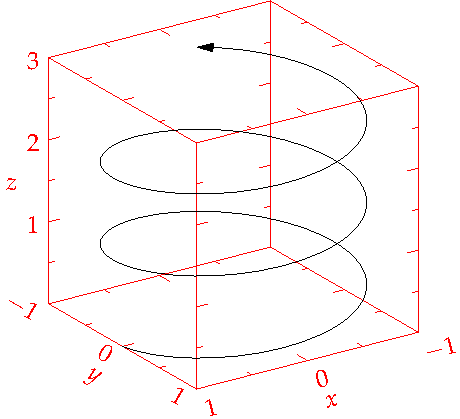
\includegraphics[width=\linewidth]{helix}
  \caption{This is a margin figure.  The helix is defined by
  $x = \cos(2\pi z)$, $y = \sin(2\pi z)$, and $z = [0, 2.7]$.  The figure was
  drawn using Asymptote (\url{http://asymptote.sf.net/}).}
  \label{fig:marginfig}
\end{marginfigure}
\begin{Verbatim}
  \begin{marginfigure}
    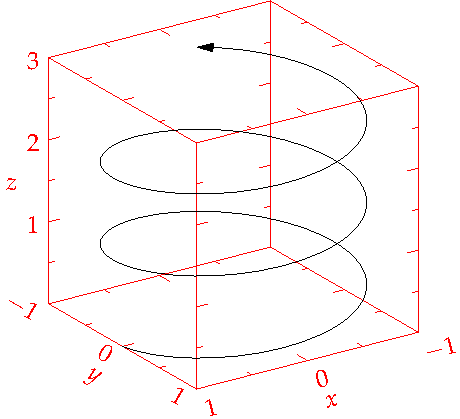
\includegraphics{helix}
    \caption{This is a margin figure.}
  \end{marginfigure}
\end{Verbatim}

The \docenv{marginfigure} and \docenv{margintable} environments accept an
optional parameter \docopt{offset} that adjusts the vertical position of the
figure or table.  See the ``\nameref{sec:sidenotes}'' section above for
examples.  The specifications are:
\begin{docspec}
  \doccmd{begin\{marginfigure\}[\docopt{offset}]}\\
  \qquad\ldots\\
  \doccmd{end\{marginfigure\}}\\
  \mbox{}\\
  \doccmd{begin\{margintable\}[\docopt{offset}]}\\
  \qquad\ldots\\
  \doccmd{end\{margintable\}}\\
\end{docspec}

Figure~\ref{fig:fullfig} is an example of the \Verb|figure*|
environment and figure~\ref{fig:textfig} is an example of the normal
\Verb|figure| environment.

\begin{figure*}[h]
  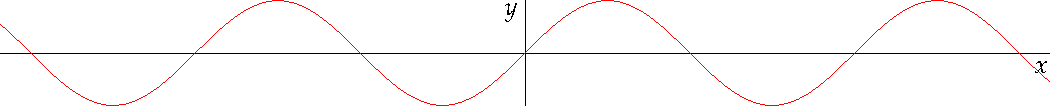
\includegraphics[width=\linewidth]{sine.pdf}%
  \caption{This graph shows $y = \sin x$ from about $x = [-10, 10]$.
  \emph{Notice that this figure takes up the full page
    width.}}%
  \label{fig:fullfig}%
\end{figure*}

\begin{figure}
  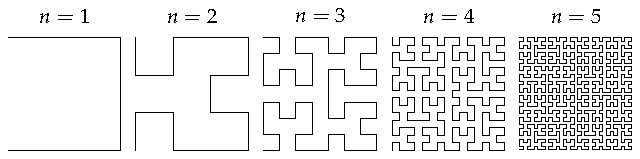
\includegraphics{hilbertcurves.pdf}
  %  \checkparity This is an \pageparity\ page.%
  \caption{Hilbert curves of various degrees $n$.
    \emph{Notice that this figure only takes up the main textblock width.}}
  \label{fig:textfig}
  %\zsavepos{pos:textfig}
  \setfloatalignment{b}
\end{figure}

Table~\ref{tab:normaltab} shows table created with the \docpkg{booktabs}
package.  Notice the lack of vertical rules---they serve only to clutter
the table's data.

\begin{table}[ht]
  \centering
  \fontfamily{ppl}\selectfont
  \begin{tabular}{ll}
    \toprule
    Margin                    & Length                          \\
    \midrule
    Paper width               & \unit[8\nicefrac{1}{2}]{inches} \\
    Paper height              & \unit[11]{inches}               \\
    Textblock width           & \unit[6\nicefrac{1}{2}]{inches} \\
    Textblock/sidenote gutter & \unit[\nicefrac{3}{8}]{inches}  \\
    Sidenote width            & \unit[2]{inches}                \\
    \bottomrule
  \end{tabular}
  \caption{Here are the dimensions of the various margins used in the
    Tufte-handout class.}
  \label{tab:normaltab}
  %\zsavepos{pos:normaltab}
\end{table}

\section{Full-width text blocks}

In addition to the new float types, there is a \docenv{fullwidth}
environment that stretches across the main text block and the sidenotes
area.

\begin{Verbatim}
  \begin{fullwidth}
    Lorem ipsum dolor sit amet...
  \end{fullwidth}
\end{Verbatim}

\begin{fullwidth}
  \small\itshape\lipsum[1]
\end{fullwidth}

\section{Typography}\label{sec:typography}

\subsection{Typefaces}\label{sec:typefaces}
If the Palatino, \textsf{Helvetica}, and \texttt{Bera Mono} typefaces are
installed, this style
will use them automatically.  Otherwise, we'll fall back on the Computer Modern
typefaces.

\subsection{Letterspacing}\label{sec:letterspacing}
This document class includes two new commands and some improvements on
existing commands for letterspacing.

When setting strings of \allcaps{ALL CAPS} or \smallcaps{small caps}, the
letter\-spacing---that is, the spacing between the letters---should be
increased slightly.\cite{Bringhurst2005}  The \Verb|\allcaps| command has
proper letterspacing for
strings of \allcaps{FULL CAPITAL LETTERS}, and the \Verb|\smallcaps| command
has letterspacing for \smallcaps{small capital letters}.  These commands
will also automatically convert the case of the text to upper- or
lowercase, respectively.

The \Verb|\textsc| command has also been redefined to include
letterspacing.	The case of the \Verb|\textsc| argument is left as is,
however.  This allows one to use both uppercase and lowercase letters:
\textsc{The Initial Letters Of The Words In This Sentence Are Capitalized.}

\section{Installation}\label{sec:installation}
To install the Tufte-\LaTeX\ classes, simply drop the
following files into the same directory as your \texttt{.tex}
file:
\begin{quote}
  \ttfamily
  tufte-book.cls\\
  tufte-common.def\\
  tufte-handout.cls\\
  tufte.bst
\end{quote}

% TODO add instructions for installing it globally

\section{More Documentation}\label{sec:more-doc}
For more documentation on the Tufte-\LaTeX{} document classes (including
commands not
mentioned in this handout), please see the sample book.

\section{Support}\label{sec:support}

The website for the Tufte-\LaTeX\ packages is located at
\url{https://github.com/Tufte-LaTeX/tufte-latex}.  On our website, you'll find
links to our \smallcaps{svn} repository, mailing lists, bug tracker, and
documentation.

\bibliography{sample-handout}
\bibliographystyle{plainnat}

\end{document}
